\documentclass[twoside]{book}

% Packages required by doxygen
\usepackage{fixltx2e}
\usepackage{calc}
\usepackage{doxygen}
\usepackage[export]{adjustbox} % also loads graphicx
\usepackage{graphicx}
\usepackage[utf8]{inputenc}
\usepackage{makeidx}
\usepackage{multicol}
\usepackage{multirow}
\PassOptionsToPackage{warn}{textcomp}
\usepackage{textcomp}
\usepackage[nointegrals]{wasysym}
\usepackage[table]{xcolor}

% Font selection
\usepackage[T1]{fontenc}
\usepackage[scaled=.90]{helvet}
\usepackage{courier}
\usepackage{amssymb}
\usepackage{sectsty}
\renewcommand{\familydefault}{\sfdefault}
\allsectionsfont{%
  \fontseries{bc}\selectfont%
  \color{darkgray}%
}
\renewcommand{\DoxyLabelFont}{%
  \fontseries{bc}\selectfont%
  \color{darkgray}%
}
\newcommand{\+}{\discretionary{\mbox{\scriptsize$\hookleftarrow$}}{}{}}

% Page & text layout
\usepackage{geometry}
\geometry{%
  letterpaper,%
  top=2.5cm,%
  bottom=2.5cm,%
  left=2.5cm,%
  right=2.5cm%
}
\tolerance=750
\hfuzz=15pt
\hbadness=750
\setlength{\emergencystretch}{15pt}
\setlength{\parindent}{0cm}
\setlength{\parskip}{3ex plus 2ex minus 2ex}
\makeatletter
\renewcommand{\paragraph}{%
  \@startsection{paragraph}{4}{0ex}{-1.0ex}{1.0ex}{%
    \normalfont\normalsize\bfseries\SS@parafont%
  }%
}
\renewcommand{\subparagraph}{%
  \@startsection{subparagraph}{5}{0ex}{-1.0ex}{1.0ex}{%
    \normalfont\normalsize\bfseries\SS@subparafont%
  }%
}
\makeatother

% Headers & footers
\usepackage{fancyhdr}
\pagestyle{fancyplain}
\fancyhead[LE]{\fancyplain{}{\bfseries\thepage}}
\fancyhead[CE]{\fancyplain{}{}}
\fancyhead[RE]{\fancyplain{}{\bfseries\leftmark}}
\fancyhead[LO]{\fancyplain{}{\bfseries\rightmark}}
\fancyhead[CO]{\fancyplain{}{}}
\fancyhead[RO]{\fancyplain{}{\bfseries\thepage}}
\fancyfoot[LE]{\fancyplain{}{}}
\fancyfoot[CE]{\fancyplain{}{}}
\fancyfoot[RE]{\fancyplain{}{\bfseries\scriptsize Generated by Doxygen }}
\fancyfoot[LO]{\fancyplain{}{\bfseries\scriptsize Generated by Doxygen }}
\fancyfoot[CO]{\fancyplain{}{}}
\fancyfoot[RO]{\fancyplain{}{}}
\renewcommand{\footrulewidth}{0.4pt}
\renewcommand{\chaptermark}[1]{%
  \markboth{#1}{}%
}
\renewcommand{\sectionmark}[1]{%
  \markright{\thesection\ #1}%
}

% Indices & bibliography
\usepackage{natbib}
\usepackage[titles]{tocloft}
\setcounter{tocdepth}{3}
\setcounter{secnumdepth}{5}
\makeindex

% Packages requested by user
\usepackage{times}

% Hyperlinks (required, but should be loaded last)
\usepackage{ifpdf}
\ifpdf
  \usepackage[pdftex,pagebackref=true]{hyperref}
\else
  \usepackage[ps2pdf,pagebackref=true]{hyperref}
\fi
\hypersetup{%
  colorlinks=true,%
  linkcolor=blue,%
  citecolor=blue,%
  unicode%
}

% Custom commands
\newcommand{\clearemptydoublepage}{%
  \newpage{\pagestyle{empty}\cleardoublepage}%
}

\usepackage{caption}
\captionsetup{labelsep=space,justification=centering,font={bf},singlelinecheck=off,skip=4pt,position=top}

%===== C O N T E N T S =====

\begin{document}

% Titlepage & ToC
\hypersetup{pageanchor=false,
             bookmarksnumbered=true,
             pdfencoding=unicode
            }
\pagenumbering{alph}
\begin{titlepage}
\vspace*{7cm}
\begin{center}%
{\Large Hardware Locality (hwloc) \\[1ex]\large 2.\+5.\+0a1-\/git }\\
\vspace*{1cm}
{\large Generated by Doxygen 1.8.13}\\
\end{center}
\end{titlepage}
\clearemptydoublepage
\pagenumbering{roman}
\tableofcontents
\clearemptydoublepage
\pagenumbering{arabic}
\hypersetup{pageanchor=true}

%--- Begin generated contents ---
\chapter{Hardware Locality}
\label{index}\hypertarget{index}{}\section*{Portable abstraction of parallel architectures for high-\/performance computing}





 \hypertarget{index_common_introduction}{}\section{Introduction}\label{index_common_introduction}
The Hardware Locality (hwloc) software project aims at easing the process of discovering hardware resources in parallel architectures. It offers command-\/line tools and a C A\+PI for consulting these resources, their locality, attributes, and interconnection. hwloc primarily aims at helping high-\/performance computing (H\+PC) applications, but is also applicable to any project seeking to exploit code and/or data locality on modern computing platforms.

hwloc is actually made of two subprojects distributed together\+: 
\begin{DoxyItemize}
\item {\bfseries The original hwloc project for describing the internals of computing nodes}. It is described in details starting at section \hyperlink{a00379}{Hardware Locality (hwloc) Introduction}.  
\item {\bfseries The network-\/oriented companion called netloc (Network Locality)}, described in details starting with section \hyperlink{a00396}{Network Locality (netloc)}.  
\end{DoxyItemize}



Netloc may be disabled, but the original hwloc cannot. Both hwloc and netloc A\+P\+Is are documented after these sections.

 \hypertarget{index_common_installation}{}\section{Installation}\label{index_common_installation}
hwloc (\href{https://www.open-mpi.org/projects/hwloc/}{\tt https\+://www.\+open-\/mpi.\+org/projects/hwloc/}) is available under the B\+SD license. It is hosted as a sub-\/project of the overall Open M\+PI project (\href{https://www.open-mpi.org/}{\tt https\+://www.\+open-\/mpi.\+org/}). Note that hwloc does not require any functionality from Open M\+PI -- it is a wholly separate (and much smaller!) project and code base. It just happens to be hosted as part of the overall Open M\+PI project.\hypertarget{index_basic_installation}{}\subsection{Basic Installation}\label{index_basic_installation}
Installation is the fairly common G\+N\+U-\/based process\+:

\begin{DoxyVerb}shell$ ./configure --prefix=...
shell$ make
shell$ make install
\end{DoxyVerb}


hwloc-\/ and netloc-\/specific configure options and requirements are documented in sections \hyperlink{a00379_hwloc_installation}{hwloc Installation} and \hyperlink{a00396_netloc_installation}{Netloc Installation} respectively.

Also note that if you install supplemental libraries in non-\/standard locations, hwloc\textquotesingle{}s configure script may not be able to find them without some help. You may need to specify additional C\+P\+P\+F\+L\+A\+GS, L\+D\+F\+L\+A\+GS, or P\+K\+G\+\_\+\+C\+O\+N\+F\+I\+G\+\_\+\+P\+A\+TH values on the configure command line.

For example, if libpciaccess was installed into /opt/pciaccess, hwloc\textquotesingle{}s configure script may not find it be default. Try adding P\+K\+G\+\_\+\+C\+O\+N\+F\+I\+G\+\_\+\+P\+A\+TH to the ./configure command line, like this\+:

\begin{DoxyVerb}./configure PKG_CONFIG_PATH=/opt/pciaccess/lib/pkgconfig ...
\end{DoxyVerb}


Running the \char`\"{}lstopo\char`\"{} tool is a good way to check as a graphical output whether hwloc properly detected the architecture of your node. Netloc command-\/line tools can be used to display the network topology interconnecting your nodes.\hypertarget{index_gitclone_installation}{}\subsection{Installing from a Git clone}\label{index_gitclone_installation}
Additionally, the code can be directly cloned from Git\+:

\begin{DoxyVerb}shell$ git clone https://github.com/open-mpi/hwloc.git
shell$ cd hwloc
shell$ ./autogen.sh
\end{DoxyVerb}


Note that G\+NU Autoconf $>$=2.\+63, Automake $>$=1.\+11 and Libtool $>$=2.\+2.\+6 are required when building from a Git clone.

Nightly development snapshots are available on the web site, they can be configured and built without any need for Git or G\+NU Autotools.

 \hypertarget{index_bugs}{}\section{Questions and Bugs}\label{index_bugs}
Bugs should be reported in the tracker (\href{https://github.com/open-mpi/hwloc/issues}{\tt https\+://github.\+com/open-\/mpi/hwloc/issues}). Opening a new issue automatically displays lots of hints about how to debug and report issues.

Questions may be sent to the users or developers mailing lists (\href{https://www.open-mpi.org/community/lists/hwloc.php}{\tt https\+://www.\+open-\/mpi.\+org/community/lists/hwloc.\+php}).

There is also a {\ttfamily \#hwloc} I\+RC channel on Freenode ({\ttfamily irc.\+freenode.\+net}). 
\chapter{Hardware Locality (hwloc) Introduction}
\label{a00379}
\Hypertarget{a00379}
\section*{Portable abstraction of hierarchical architectures for high-\/performance computing}





 See also \hyperlink{a00379_further_reading}{Further Reading}  for links to more sections about hwloc concepts. 

 \hypertarget{a00379_hwloc_summary}{}\section{hwloc Summary}\label{a00379_hwloc_summary}
hwloc provides command line tools and a C A\+PI to obtain the hierarchical map of key computing elements within a node, such as\+: N\+U\+MA memory nodes, shared caches, processor packages, dies and cores, processing units (logical processors or \char`\"{}threads\char`\"{}) and even I/O devices. hwloc also gathers various attributes such as cache and memory information, and is portable across a variety of different operating systems and platforms.

hwloc primarily aims at helping high-\/performance computing (H\+PC) applications, but is also applicable to any project seeking to exploit code and/or data locality on modern computing platforms.

hwloc supports the following operating systems\+:


\begin{DoxyItemize}
\item Linux (including old kernels not having sysfs topology information, with knowledge of cpusets, Scale\+MP v\+S\+MP support, etc.) on all supported hardware, including Intel Xeon Phi and Numa\+Scale Numa\+Connect. 
\item Solaris (with support for processor sets and logical domains) 
\item A\+IX 
\item Darwin / OS X 
\item Free\+B\+SD and its variants (such as k\+Free\+B\+S\+D/\+G\+NU) 
\item Net\+B\+SD 
\item H\+P-\/\+UX 
\item Microsoft Windows 
\item I\+BM Blue\+Gene/Q Compute Node Kernel (C\+NK) 
\end{DoxyItemize}

Since it uses standard Operating System information, hwloc\textquotesingle{}s support is mostly independant from the processor type (x86, powerpc, ...) and just relies on the Operating System support. The main exception is B\+SD operating systems (Net\+B\+SD, Free\+B\+SD, etc.) because they do not provide support topology information, hence hwloc uses an x86-\/only C\+P\+U\+I\+D-\/based backend (which can be used for other O\+Ses too, see the \hyperlink{a00392}{Components and plugins} section).

To check whether hwloc works on a particular machine, just try to build it and run {\ttfamily lstopo} or {\ttfamily lstopo-\/no-\/graphics}. If some things do not look right (e.\+g. bogus or missing cache information), see \hyperlink{index_bugs}{Questions and Bugs}.

hwloc only reports the number of processors on unsupported operating systems; no topology information is available.

For development and debugging purposes, hwloc also offers the ability to work on \char`\"{}fake\char`\"{} topologies\+:


\begin{DoxyItemize}
\item Symmetrical tree of resources generated from a list of level arities, see \hyperlink{a00389}{Synthetic topologies}. 
\item Remote machine simulation through the gathering of topology as X\+ML files, see \hyperlink{a00388}{Importing and exporting topologies from/to X\+ML files}. 
\end{DoxyItemize}

hwloc can display the topology in a human-\/readable format, either in graphical mode (X11), or by exporting in one of several different formats, including\+: plain text, La\+TeX tikzpicture, P\+DF, P\+NG, and F\+IG (see \hyperlink{a00379_cli_examples}{Command-\/line Examples} below). Note that some of the export formats require additional support libraries.

hwloc offers a programming interface for manipulating topologies and objects. It also brings a powerful C\+PU bitmap A\+PI that is used to describe topology objects location on physical/logical processors. See the \hyperlink{a00379_interface}{Programming Interface} below. It may also be used to binding applications onto certain cores or memory nodes. Several utility programs are also provided to ease command-\/line manipulation of topology objects, binding of processes, and so on.

Perl bindings are available from Bernd Kallies on \href{http://search.cpan.org/~bka/Sys-Hwloc-0.10/}{\tt C\+P\+AN}.

Python bindings are available from Guy Streeter\+: 
\begin{DoxyItemize}
\item \href{http://people.redhat.com/streeter/}{\tt Fedora R\+PM and tarball}. 
\item \href{git://git.fedorahosted.org/python-hwloc.git}{\tt git tree} (\href{http://git.fedorahosted.org/git/python-hwloc.git}{\tt html}). 
\end{DoxyItemize}

 \hypertarget{a00379_hwloc_installation}{}\section{hwloc Installation}\label{a00379_hwloc_installation}
The generic installation procedure for both hwloc and netloc is described in \hyperlink{index_common_installation}{Installation}.

The hwloc command-\/line tool \char`\"{}lstopo\char`\"{} produces human-\/readable topology maps, as mentioned above. It can also export maps to the \char`\"{}fig\char`\"{} file format. Support for P\+DF, Postscript, and P\+NG exporting is provided if the \char`\"{}\+Cairo\char`\"{} development package (usually {\ttfamily cairo-\/devel} or {\ttfamily libcairo2-\/dev}) can be found in \char`\"{}lstopo\char`\"{} when hwloc is configured and build.

The hwloc core may also benefit from the following development packages\+: 
\begin{DoxyItemize}
\item libpciaccess for full I/O device discovery ({\ttfamily libpciaccess-\/devel} or {\ttfamily libpciaccess-\/dev} package). On Linux, P\+CI discovery may still be performed (without vendor/device names) even if libpciaccess cannot be used. 


\item A\+MD or N\+V\+I\+D\+IA Open\+CL implementations for Open\+CL device discovery.  
\item the N\+V\+I\+D\+IA C\+U\+DA Toolkit for C\+U\+DA device discovery. It\textquotesingle{}s installation path may be specified at configure time with {\ttfamily --with-\/cuda=/path/to/cuda}.  
\item the N\+V\+I\+D\+IA Management Library (N\+V\+ML) for N\+V\+ML device discovery. It is included in C\+U\+DA since version 8.\+0. Older N\+V\+ML releases were available within the N\+V\+I\+D\+IA G\+PU Deployment Kit from \href{https://developer.nvidia.com/gpu-deployment-kit}{\tt https\+://developer.\+nvidia.\+com/gpu-\/deployment-\/kit} .  
\item the N\+V-\/\+C\+O\+N\+T\+R\+OL X extension library (N\+V\+Ctrl) for N\+V\+I\+D\+IA display discovery. The relevant development package is usually {\ttfamily lib\+X\+N\+V\+Ctrl-\/devel} or {\ttfamily libxnvctrl-\/dev}. It is also available within nvidia-\/settings from \href{ftp://download.nvidia.com/XFree86/nvidia-settings/}{\tt ftp\+://download.\+nvidia.\+com/\+X\+Free86/nvidia-\/settings/} and \href{https://github.com/NVIDIA/nvidia-settings/}{\tt https\+://github.\+com/\+N\+V\+I\+D\+I\+A/nvidia-\/settings/} .  
\item the A\+MD R\+O\+Cm S\+MI library for R\+S\+MI device discovery. The relevant development package is usually {\ttfamily rocm-\/smi-\/lib64} or {\ttfamily librocm-\/smi-\/dev}.  
\item libxml2 for full X\+ML import/export support (otherwise, the internal minimalistic parser will only be able to import X\+ML files that were exported by the same hwloc release). See \hyperlink{a00388}{Importing and exporting topologies from/to X\+ML files} for details. The relevant development package is usually {\ttfamily libxml2-\/devel} or {\ttfamily libxml2-\/dev}.  
\item libudev on Linux for easier discovery of OS device information (otherwise hwloc will try to manually parse udev raw files). The relevant development package is usually {\ttfamily libudev-\/devel} or {\ttfamily libudev-\/dev}.  
\item libtool\textquotesingle{}s ltdl library for dynamic plugin loading if the native dlopen cannot be used. The relevant development package is usually {\ttfamily libtool-\/ltdl-\/devel} or {\ttfamily libltdl-\/dev}.  
\end{DoxyItemize}

P\+CI and X\+ML support may be statically built inside the main hwloc library, or as separate dynamically-\/loaded plugins (see the \hyperlink{a00392}{Components and plugins} section).

Note that because of the possibility of G\+PL taint, the {\ttfamily pciutils} library {\ttfamily libpci} will not be used (remember that hwloc is B\+S\+D-\/licensed).

 \hypertarget{a00379_cli_examples}{}\section{Command-\/line Examples}\label{a00379_cli_examples}
On a 4-\/package 2-\/core machine with hyper-\/threading, the {\ttfamily lstopo} tool may show the following graphical output\+:

 
\begin{DoxyImageNoCaption}
  \mbox{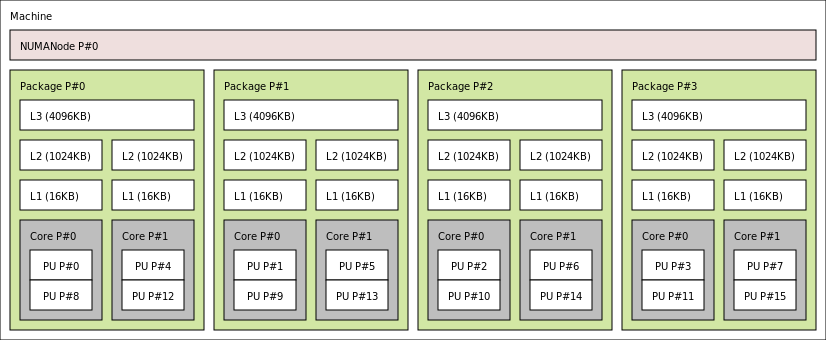
\includegraphics[width=\textwidth]{dudley.png}}
\end{DoxyImageNoCaption}


Here\textquotesingle{}s the equivalent output in textual form\+:

\begin{DoxyVerb}Machine
  NUMANode L#0 (P#0)
  Package L#0 + L3 L#0 (4096KB)
    L2 L#0 (1024KB) + L1 L#0 (16KB) + Core L#0
      PU L#0 (P#0)
      PU L#1 (P#8)
    L2 L#1 (1024KB) + L1 L#1 (16KB) + Core L#1
      PU L#2 (P#4)
      PU L#3 (P#12)
  Package L#1 + L3 L#1 (4096KB)
    L2 L#2 (1024KB) + L1 L#2 (16KB) + Core L#2
      PU L#4 (P#1)
      PU L#5 (P#9)
    L2 L#3 (1024KB) + L1 L#3 (16KB) + Core L#3
      PU L#6 (P#5)
      PU L#7 (P#13)
  Package L#2 + L3 L#2 (4096KB)
    L2 L#4 (1024KB) + L1 L#4 (16KB) + Core L#4
      PU L#8 (P#2)
      PU L#9 (P#10)
    L2 L#5 (1024KB) + L1 L#5 (16KB) + Core L#5
      PU L#10 (P#6)
      PU L#11 (P#14)
  Package L#3 + L3 L#3 (4096KB)
    L2 L#6 (1024KB) + L1 L#6 (16KB) + Core L#6
      PU L#12 (P#3)
      PU L#13 (P#11)
    L2 L#7 (1024KB) + L1 L#7 (16KB) + Core L#7
      PU L#14 (P#7)
      PU L#15 (P#15)
\end{DoxyVerb}


Note that there is also an equivalent output in X\+ML that is meant for exporting/importing topologies but it is hardly readable to human-\/beings (see \hyperlink{a00388}{Importing and exporting topologies from/to X\+ML files} for details).

On a 4-\/package 2-\/core Opteron N\+U\+MA machine (with two core cores disallowed by the administrator), the {\ttfamily lstopo} tool may show the following graphical output (with {\ttfamily -\/-\/disallowed} for displaying disallowed objects)\+:

 
\begin{DoxyImageNoCaption}
  \mbox{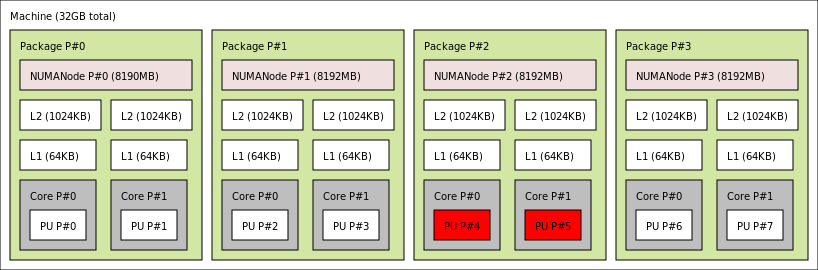
\includegraphics[width=\textwidth]{hagrid.png}}
\end{DoxyImageNoCaption}


Here\textquotesingle{}s the equivalent output in textual form\+:

\begin{DoxyVerb}Machine (32GB total)
  Package L#0
    NUMANode L#0 (P#0 8190MB)
    L2 L#0 (1024KB) + L1 L#0 (64KB) + Core L#0 + PU L#0 (P#0)
    L2 L#1 (1024KB) + L1 L#1 (64KB) + Core L#1 + PU L#1 (P#1)
  Package L#1
    NUMANode L#1 (P#1 8192MB)
    L2 L#2 (1024KB) + L1 L#2 (64KB) + Core L#2 + PU L#2 (P#2)
    L2 L#3 (1024KB) + L1 L#3 (64KB) + Core L#3 + PU L#3 (P#3)
  Package L#2
    NUMANode L#2 (P#2 8192MB)
    L2 L#4 (1024KB) + L1 L#4 (64KB) + Core L#4 + PU L#4 (P#4)
    L2 L#5 (1024KB) + L1 L#5 (64KB) + Core L#5 + PU L#5 (P#5)
  Package L#3
    NUMANode L#3 (P#3 8192MB)
    L2 L#6 (1024KB) + L1 L#6 (64KB) + Core L#6 + PU L#6 (P#6)
    L2 L#7 (1024KB) + L1 L#7 (64KB) + Core L#7 + PU L#7 (P#7)
\end{DoxyVerb}


On a 2-\/package quad-\/core Xeon (pre-\/\+Nehalem, with 2 dual-\/core dies into each package)\+:

 
\begin{DoxyImageNoCaption}
  \mbox{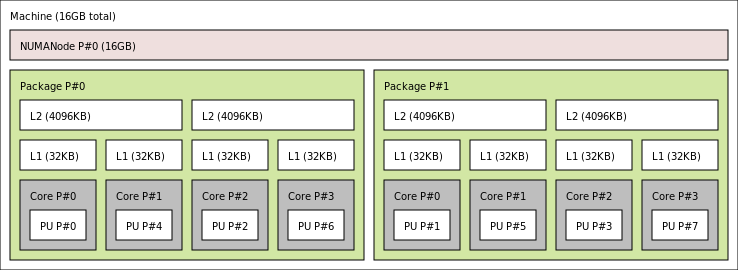
\includegraphics[width=\textwidth]{emmett.png}}
\end{DoxyImageNoCaption}


Here\textquotesingle{}s the same output in textual form\+:

\begin{DoxyVerb}Machine (total 16GB)
  NUMANode L#0 (P#0 16GB)
  Package L#0
    L2 L#0 (4096KB)
      L1 L#0 (32KB) + Core L#0 + PU L#0 (P#0)
      L1 L#1 (32KB) + Core L#1 + PU L#1 (P#4)
    L2 L#1 (4096KB)
      L1 L#2 (32KB) + Core L#2 + PU L#2 (P#2)
      L1 L#3 (32KB) + Core L#3 + PU L#3 (P#6)
  Package L#1
    L2 L#2 (4096KB)
      L1 L#4 (32KB) + Core L#4 + PU L#4 (P#1)
      L1 L#5 (32KB) + Core L#5 + PU L#5 (P#5)
    L2 L#3 (4096KB)
      L1 L#6 (32KB) + Core L#6 + PU L#6 (P#3)
      L1 L#7 (32KB) + Core L#7 + PU L#7 (P#7)
\end{DoxyVerb}


 \hypertarget{a00379_interface}{}\section{Programming Interface}\label{a00379_interface}
The basic interface is available in \hyperlink{a00119_source}{hwloc.\+h}. Some higher-\/level functions are available in \hyperlink{a00122_source}{hwloc/helper.\+h} to reduce the need to manually manipulate objects and follow links between them. Documentation for all these is provided later in this document. Developers may also want to look at hwloc/inlines.\+h which contains the actual inline code of some \hyperlink{a00119_source}{hwloc.\+h} routines, and at this document, which provides good higher-\/level topology traversal examples.

To precisely define the vocabulary used by hwloc, a \hyperlink{a00380}{Terms and Definitions} section is available and should probably be read first.

Each hwloc object contains a cpuset describing the list of processing units that it contains. These bitmaps may be used for \hyperlink{a00190}{C\+PU binding} and \hyperlink{a00191}{Memory binding}. hwloc offers an extensive bitmap manipulation interface in \hyperlink{a00125_source}{hwloc/bitmap.\+h}.

Moreover, hwloc also comes with additional helpers for interoperability with several commonly used environments. See the \hyperlink{a00390}{Interoperability With Other Software} section for details.

The complete A\+PI documentation is available in a full set of H\+T\+ML pages, man pages, and self-\/contained P\+DF files (formatted for both both US letter and A4 formats) in the source tarball in doc/doxygen-\/doc/.

{\bfseries N\+O\+TE\+:} If you are building the documentation from a Git clone, you will need to have Doxygen and pdflatex installed -- the documentation will be built during the normal \char`\"{}make\char`\"{} process. The documentation is installed during \char`\"{}make install\char`\"{} to \$prefix/share/doc/hwloc/ and your systems default man page tree (under \$prefix, of course).\hypertarget{a00379_portability}{}\subsection{Portability}\label{a00379_portability}
Operating System have varying support for C\+PU and memory binding, e.\+g. while some Operating Systems provide interfaces for all kinds of C\+PU and memory bindings, some others provide only interfaces for a limited number of kinds of C\+PU and memory binding, and some do not provide any binding interface at all. Hwloc\textquotesingle{}s binding functions would then simply return the E\+N\+O\+S\+YS error (Function not implemented), meaning that the underlying Operating System does not provide any interface for them. \hyperlink{a00190}{C\+PU binding} and \hyperlink{a00191}{Memory binding} provide more information on which hwloc binding functions should be preferred because interfaces for them are usually available on the supported Operating Systems.

Similarly, the ability of reporting topology information varies from one platform to another. As shown in \hyperlink{a00379_cli_examples}{Command-\/line Examples}, hwloc can obtain information on a wide variety of hardware topologies. However, some platforms and/or operating system versions will only report a subset of this information. For example, on an P\+P\+C64-\/based system with 8 cores (each with 2 hardware threads) running a default 2.\+6.\+18-\/based kernel from R\+H\+EL 5.\+4, hwloc is only able to glean information about N\+U\+MA nodes and processor units (P\+Us). No information about caches, packages, or cores is available.

Here\textquotesingle{}s the graphical output from lstopo on this platform when Simultaneous Multi-\/\+Threading (S\+MT) is enabled\+:

 
\begin{DoxyImageNoCaption}
  \mbox{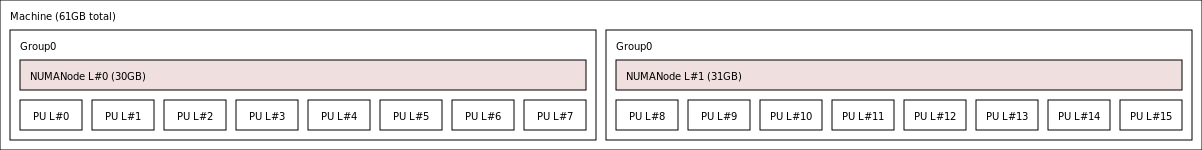
\includegraphics[width=\textwidth]{ppc64-with-smt.png}}
\end{DoxyImageNoCaption}


And here\textquotesingle{}s the graphical output from lstopo on this platform when S\+MT is disabled\+:

 
\begin{DoxyImageNoCaption}
  \mbox{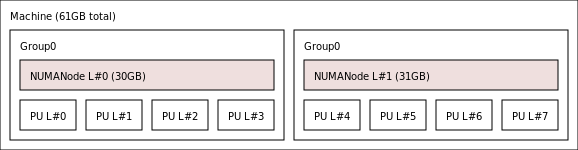
\includegraphics[width=.5\textwidth]{ppc64-without-smt.png}}
\end{DoxyImageNoCaption}


Notice that hwloc only sees half the P\+Us when S\+MT is disabled. PU L\#6, for example, seems to change location from N\+U\+MA node \#0 to \#1. In reality, no P\+Us \char`\"{}moved\char`\"{} -- they were simply re-\/numbered when hwloc only saw half as many (see also Logical index in \hyperlink{a00380_termsanddefs_indexes}{Indexes and Sets}). Hence, PU L\#6 in the S\+M\+T-\/disabled picture probably corresponds to PU L\#12 in the S\+M\+T-\/enabled picture.

This same \char`\"{}\+P\+Us have disappeared\char`\"{} effect can be seen on other platforms -- even platforms / O\+Ss that provide much more information than the above P\+P\+C64 system. This is an unfortunate side-\/effect of how operating systems report information to hwloc.

Note that upgrading the Linux kernel on the same P\+P\+C64 system mentioned above to 2.\+6.\+34, hwloc is able to discover all the topology information. The following picture shows the entire topology layout when S\+MT is enabled\+:

 
\begin{DoxyImageNoCaption}
  \mbox{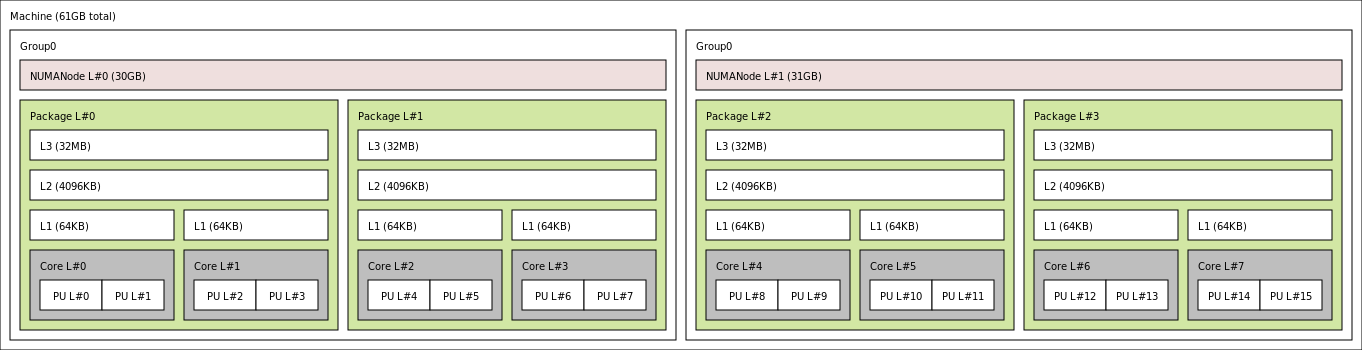
\includegraphics[width=\textwidth]{ppc64-full-with-smt.png}}
\end{DoxyImageNoCaption}


Developers using the hwloc A\+PI or X\+ML output for portable applications should therefore be extremely careful to not make any assumptions about the structure of data that is returned. For example, per the above reported P\+PC topology, it is not safe to assume that P\+Us will always be descendants of cores.

Additionally, future hardware may insert new topology elements that are not available in this version of hwloc. Long-\/lived applications that are meant to span multiple different hardware platforms should also be careful about making structure assumptions. For example, a new element may someday exist between a core and a PU.\hypertarget{a00379_interface_example}{}\subsection{A\+P\+I Example}\label{a00379_interface_example}
The following small C example (available in the source tree as ``doc/examples/hwloc-\/hello.c\textquotesingle{}\textquotesingle{}) prints the topology of the machine and performs some thread and memory binding. More examples are available in the doc/examples/ directory of the source tree.


\begin{DoxyCodeInclude}
\textcolor{comment}{/* Example hwloc API program.}
\textcolor{comment}{ *}
\textcolor{comment}{ * See other examples under doc/examples/ in the source tree}
\textcolor{comment}{ * for more details.}
\textcolor{comment}{ *}
\textcolor{comment}{ * Copyright © 2009-2016 Inria.  All rights reserved.}
\textcolor{comment}{ * Copyright © 2009-2011 Université Bordeaux}
\textcolor{comment}{ * Copyright © 2009-2010 Cisco Systems, Inc.  All rights reserved.}
\textcolor{comment}{ * See COPYING in top-level directory.}
\textcolor{comment}{ *}
\textcolor{comment}{ * hwloc-hello.c}
\textcolor{comment}{ */}

\textcolor{preprocessor}{#include "hwloc.h"}

\textcolor{preprocessor}{#include <errno.h>}
\textcolor{preprocessor}{#include <stdio.h>}
\textcolor{preprocessor}{#include <string.h>}

\textcolor{keyword}{static} \textcolor{keywordtype}{void} print\_children(\hyperlink{a00186_ga9d1e76ee15a7dee158b786c30b6a6e38}{hwloc\_topology\_t} topology, 
      \hyperlink{a00238}{hwloc\_obj\_t} obj,
                           \textcolor{keywordtype}{int} depth)
\{
    \textcolor{keywordtype}{char} type[32], attr[1024];
    \textcolor{keywordtype}{unsigned} i;

    \hyperlink{a00188_gadb8765c260edea80c52cd06a76639ba4}{hwloc\_obj\_type\_snprintf}(type, \textcolor{keyword}{sizeof}(type), obj, 0);
    printf(\textcolor{stringliteral}{"%*s%s"}, 2*depth, \textcolor{stringliteral}{""}, type);
    \textcolor{keywordflow}{if} (obj->\hyperlink{a00238_a61a7a80a68eaccbaaa28269e678c81a9}{os\_index} != (\textcolor{keywordtype}{unsigned}) -1)
      printf(\textcolor{stringliteral}{"#%u"}, obj->\hyperlink{a00238_a61a7a80a68eaccbaaa28269e678c81a9}{os\_index});
    \hyperlink{a00188_ga870e876931c282a1c7aee2f031912ce3}{hwloc\_obj\_attr\_snprintf}(attr, \textcolor{keyword}{sizeof}(attr), obj, \textcolor{stringliteral}{" "}, 0);
    \textcolor{keywordflow}{if} (*attr)
      printf(\textcolor{stringliteral}{"(%s)"}, attr);
    printf(\textcolor{stringliteral}{"\(\backslash\)n"});
    \textcolor{keywordflow}{for} (i = 0; i < obj->\hyperlink{a00238_aac3f6da35c9b57599909a44ce2b716c1}{arity}; i++) \{
        print\_children(topology, obj->\hyperlink{a00238_a04d05403da37bfe17cd63b7c7dd07b1f}{children}[i], depth + 1);
    \}
\}

\textcolor{keywordtype}{int} main(\textcolor{keywordtype}{void})
\{
    \textcolor{keywordtype}{int} \hyperlink{a00238_a4876fd165b4fff35521f07ebd85355ed}{depth};
    \textcolor{keywordtype}{unsigned} i, n;
    \textcolor{keywordtype}{unsigned} \textcolor{keywordtype}{long} size;
    \textcolor{keywordtype}{int} levels;
    \textcolor{keywordtype}{char} \textcolor{keywordtype}{string}[128];
    \textcolor{keywordtype}{int} topodepth;
    \textcolor{keywordtype}{void} *m;
    \hyperlink{a00186_ga9d1e76ee15a7dee158b786c30b6a6e38}{hwloc\_topology\_t} topology;
    \hyperlink{a00183_ga4bbf39b68b6f568fb92739e7c0ea7801}{hwloc\_cpuset\_t} \hyperlink{a00238_a67925e0f2c47f50408fbdb9bddd0790f}{cpuset};
    \hyperlink{a00238}{hwloc\_obj\_t} obj;

    \textcolor{comment}{/* Allocate and initialize topology object. */}
    \hyperlink{a00186_ga03fd4a16d8b9ee1ffc32b25fd2f6bdfa}{hwloc\_topology\_init}(&topology);

    \textcolor{comment}{/* ... Optionally, put detection configuration here to ignore}
\textcolor{comment}{       some objects types, define a synthetic topology, etc....}
\textcolor{comment}{}
\textcolor{comment}{       The default is to detect all the objects of the machine that}
\textcolor{comment}{       the caller is allowed to access.  See Configure Topology}
\textcolor{comment}{       Detection. */}

    \textcolor{comment}{/* Perform the topology detection. */}
    \hyperlink{a00186_gabdf58d87ad77f6615fccdfe0535ff826}{hwloc\_topology\_load}(topology);

    \textcolor{comment}{/* Optionally, get some additional topology information}
\textcolor{comment}{       in case we need the topology depth later. */}
    topodepth = \hyperlink{a00187_gae54d1782ca9b54bea915f5c18a9158fa}{hwloc\_topology\_get\_depth}(topology);

    \textcolor{comment}{/*****************************************************************}
\textcolor{comment}{     * First example:}
\textcolor{comment}{     * Walk the topology with an array style, from level 0 (always}
\textcolor{comment}{     * the system level) to the lowest level (always the proc level).}
\textcolor{comment}{     *****************************************************************/}
    \textcolor{keywordflow}{for} (depth = 0; depth < topodepth; depth++) \{
        printf(\textcolor{stringliteral}{"*** Objects at level %d\(\backslash\)n"}, depth);
        \textcolor{keywordflow}{for} (i = 0; i < \hyperlink{a00187_ga1d5ceafe8130fe6e8657bf0bc666ba50}{hwloc\_get\_nbobjs\_by\_depth}(topology, depth);
             i++) \{
            \hyperlink{a00188_gadb8765c260edea80c52cd06a76639ba4}{hwloc\_obj\_type\_snprintf}(\textcolor{keywordtype}{string}, \textcolor{keyword}{sizeof}(\textcolor{keywordtype}{string}),
                                    \hyperlink{a00187_ga391f6b2613f0065673eaa4069b93d4e0}{hwloc\_get\_obj\_by\_depth}(topology, depth, i), 0);
            printf(\textcolor{stringliteral}{"Index %u: %s\(\backslash\)n"}, i, \textcolor{keywordtype}{string});
        \}
    \}

    \textcolor{comment}{/*****************************************************************}
\textcolor{comment}{     * Second example:}
\textcolor{comment}{     * Walk the topology with a tree style.}
\textcolor{comment}{     *****************************************************************/}
    printf(\textcolor{stringliteral}{"*** Printing overall tree\(\backslash\)n"});
    print\_children(topology, \hyperlink{a00187_ga2d4b12fc187dfc53b35f2fa21d21044d}{hwloc\_get\_root\_obj}(topology), 0);

    \textcolor{comment}{/*****************************************************************}
\textcolor{comment}{     * Third example:}
\textcolor{comment}{     * Print the number of packages.}
\textcolor{comment}{     *****************************************************************/}
    depth = \hyperlink{a00187_ga8bec782e21be313750da70cf7428b374}{hwloc\_get\_type\_depth}(topology, \hyperlink{a00184_ggacd37bb612667dc437d66bfb175a8dc55ab16ab8c0dbffc234921d86f3dfb63129}{HWLOC\_OBJ\_PACKAGE});
    \textcolor{keywordflow}{if} (depth == \hyperlink{a00187_ggaf4e663cf42bbe20756b849c6293ef575a0565ab92ab72cb0cec91e23003294aad}{HWLOC\_TYPE\_DEPTH\_UNKNOWN}) \{
        printf(\textcolor{stringliteral}{"*** The number of packages is unknown\(\backslash\)n"});
    \} \textcolor{keywordflow}{else} \{
        printf(\textcolor{stringliteral}{"*** %u package(s)\(\backslash\)n"},
               \hyperlink{a00187_ga1d5ceafe8130fe6e8657bf0bc666ba50}{hwloc\_get\_nbobjs\_by\_depth}(topology, depth));
    \}

    \textcolor{comment}{/*****************************************************************}
\textcolor{comment}{     * Fourth example:}
\textcolor{comment}{     * Compute the amount of cache that the first logical processor}
\textcolor{comment}{     * has above it.}
\textcolor{comment}{     *****************************************************************/}
    levels = 0;
    size = 0;
    \textcolor{keywordflow}{for} (obj = \hyperlink{a00187_ga6f414dd80a2b943967a0ac92da3181a2}{hwloc\_get\_obj\_by\_type}(topology, \hyperlink{a00184_ggacd37bb612667dc437d66bfb175a8dc55abca6887e80cb291353b0a0c1da83f661}{HWLOC\_OBJ\_PU}, 0);
         obj;
         obj = obj->\hyperlink{a00238_adc494f6aed939992be1c55cca5822900}{parent})
      \textcolor{keywordflow}{if} (\hyperlink{a00198_ga2ed589bea28711e80b92066510a5607d}{hwloc\_obj\_type\_is\_cache}(obj->\hyperlink{a00238_acc4f0803f244867e68fe0036800be5de}{type})) \{
        levels++;
        size += obj->\hyperlink{a00238_accd40e29f71f19e88db62ea3df02adc8}{attr}->\hyperlink{a00242_ab5a8ae3bf490e6b1071fea53f7382836}{cache}.\hyperlink{a00254_abe5e788943ed04302976740c829674c0}{size};
      \}
    printf(\textcolor{stringliteral}{"*** Logical processor 0 has %d caches totaling %luKB\(\backslash\)n"},
           levels, size / 1024);

    \textcolor{comment}{/*****************************************************************}
\textcolor{comment}{     * Fifth example:}
\textcolor{comment}{     * Bind to only one thread of the last core of the machine.}
\textcolor{comment}{     *}
\textcolor{comment}{     * First find out where cores are, or else smaller sets of CPUs if}
\textcolor{comment}{     * the OS doesn't have the notion of a "core".}
\textcolor{comment}{     *****************************************************************/}
    depth = \hyperlink{a00187_ga8125328e69eba709c33ea8055c12589b}{hwloc\_get\_type\_or\_below\_depth}(topology, 
      \hyperlink{a00184_ggacd37bb612667dc437d66bfb175a8dc55ac793958f330bca371aa1535de8aff45f}{HWLOC\_OBJ\_CORE});

    \textcolor{comment}{/* Get last core. */}
    obj = \hyperlink{a00187_ga391f6b2613f0065673eaa4069b93d4e0}{hwloc\_get\_obj\_by\_depth}(topology, depth,
                   \hyperlink{a00187_ga1d5ceafe8130fe6e8657bf0bc666ba50}{hwloc\_get\_nbobjs\_by\_depth}(topology, depth) - 1);
    \textcolor{keywordflow}{if} (obj) \{
        \textcolor{comment}{/* Get a copy of its cpuset that we may modify. */}
        cpuset = \hyperlink{a00205_gae679434c1a5f41d3560a8a7e2c1b0dee}{hwloc\_bitmap\_dup}(obj->\hyperlink{a00238_a67925e0f2c47f50408fbdb9bddd0790f}{cpuset});

        \textcolor{comment}{/* Get only one logical processor (in case the core is}
\textcolor{comment}{           SMT/hyper-threaded). */}
        \hyperlink{a00205_gaa611a77c092e679246afdf9a60d5db8b}{hwloc\_bitmap\_singlify}(cpuset);

        \textcolor{comment}{/* And try to bind ourself there. */}
        \textcolor{keywordflow}{if} (\hyperlink{a00190_ga80bc07473a8edf840cae17bd7ec21d48}{hwloc\_set\_cpubind}(topology, cpuset, 0)) \{
            \textcolor{keywordtype}{char} *str;
            \textcolor{keywordtype}{int} error = errno;
            \hyperlink{a00205_ga0fece972134fdecf2da9bc7a11dd827e}{hwloc\_bitmap\_asprintf}(&str, obj->\hyperlink{a00238_a67925e0f2c47f50408fbdb9bddd0790f}{cpuset});
            printf(\textcolor{stringliteral}{"Couldn't bind to cpuset %s: %s\(\backslash\)n"}, str, strerror(error));
            free(str);
        \}

        \textcolor{comment}{/* Free our cpuset copy */}
        \hyperlink{a00205_ga156130d85b3a0674d6e0e6770fe68fbe}{hwloc\_bitmap\_free}(cpuset);
    \}

    \textcolor{comment}{/*****************************************************************}
\textcolor{comment}{     * Sixth example:}
\textcolor{comment}{     * Allocate some memory on the last NUMA node, bind some existing}
\textcolor{comment}{     * memory to the last NUMA node.}
\textcolor{comment}{     *****************************************************************/}
    \textcolor{comment}{/* Get last node. There's always at least one. */}
    n = \hyperlink{a00187_ga789a3f65aedff644be64a18526a03065}{hwloc\_get\_nbobjs\_by\_type}(topology, 
      \hyperlink{a00184_ggacd37bb612667dc437d66bfb175a8dc55a9d917a3e5497950c6d8948b8e183db5a}{HWLOC\_OBJ\_NUMANODE});
    obj = \hyperlink{a00187_ga6f414dd80a2b943967a0ac92da3181a2}{hwloc\_get\_obj\_by\_type}(topology, 
      \hyperlink{a00184_ggacd37bb612667dc437d66bfb175a8dc55a9d917a3e5497950c6d8948b8e183db5a}{HWLOC\_OBJ\_NUMANODE}, n - 1);

    size = 1024*1024;
    m = \hyperlink{a00191_ga04736461780fadcf193af218c0122273}{hwloc\_alloc\_membind}(topology, size, obj->\hyperlink{a00238_a08f0d0e16c619a6e653526cbee4ffea3}{nodeset},
                            \hyperlink{a00191_ggac9764f79505775d06407b40f5e4661e8ad811fa4b2a6002c4d63695a408ffde2c}{HWLOC\_MEMBIND\_BIND}, 
      \hyperlink{a00191_ggab00475fd98815bf4fb9aaf752030e7d2a71f19fe4505f1c083dc8e6f7bdea6256}{HWLOC\_MEMBIND\_BYNODESET});
    \hyperlink{a00191_ga32dbd4f54e9e4a7179f2dde37ffe6ad7}{hwloc\_free}(topology, m, size);

    m = malloc(size);
    \hyperlink{a00191_gaf881faefe20701229f07dd7dbd0125ed}{hwloc\_set\_area\_membind}(topology, m, size, obj->\hyperlink{a00238_a08f0d0e16c619a6e653526cbee4ffea3}{nodeset},
                           \hyperlink{a00191_ggac9764f79505775d06407b40f5e4661e8ad811fa4b2a6002c4d63695a408ffde2c}{HWLOC\_MEMBIND\_BIND}, 
      \hyperlink{a00191_ggab00475fd98815bf4fb9aaf752030e7d2a71f19fe4505f1c083dc8e6f7bdea6256}{HWLOC\_MEMBIND\_BYNODESET});
    free(m);

    \textcolor{comment}{/* Destroy topology object. */}
    \hyperlink{a00186_ga9f34a640b6fd28d23699d4d084667b15}{hwloc\_topology\_destroy}(topology);

    \textcolor{keywordflow}{return} 0;
\}
\end{DoxyCodeInclude}


hwloc provides a {\ttfamily pkg-\/config} executable to obtain relevant compiler and linker flags. For example, it can be used thusly to compile applications that utilize the hwloc library (assuming G\+NU Make)\+:

\begin{DoxyVerb}CFLAGS += $(shell pkg-config --cflags hwloc)
LDLIBS += $(shell pkg-config --libs hwloc)

hwloc-hello: hwloc-hello.c
        $(CC) hwloc-hello.c $(CFLAGS) -o hwloc-hello $(LDLIBS)
\end{DoxyVerb}


On a machine 2 processor packages -- each package of which has two processing cores -- the output from running {\ttfamily hwloc-\/hello} could be something like the following\+:

\begin{DoxyVerb}shell$ ./hwloc-hello
*** Objects at level 0
Index 0: Machine
*** Objects at level 1
Index 0: Package#0
Index 1: Package#1
*** Objects at level 2
Index 0: Core#0
Index 1: Core#1
Index 2: Core#3
Index 3: Core#2
*** Objects at level 3
Index 0: PU#0
Index 1: PU#1
Index 2: PU#2
Index 3: PU#3
*** Printing overall tree
Machine
  Package#0
    Core#0
      PU#0
    Core#1
      PU#1
  Package#1
    Core#3
      PU#2
    Core#2
      PU#3
*** 2 package(s)
*** Logical processor 0 has 0 caches totaling 0KB
shell$ 
\end{DoxyVerb}


 \hypertarget{a00379_history}{}\section{History / Credits}\label{a00379_history}
hwloc is the evolution and merger of the libtopology project and the Portable Linux Processor Affinity (P\+L\+PA) (\href{https://www.open-mpi.org/projects/plpa/}{\tt https\+://www.\+open-\/mpi.\+org/projects/plpa/}) project. Because of functional and ideological overlap, these two code bases and ideas were merged and released under the name \char`\"{}hwloc\char`\"{} as an Open M\+PI sub-\/project.

libtopology was initially developed by the Inria Runtime Team-\/\+Project. P\+L\+PA was initially developed by the Open M\+PI development team as a sub-\/project. Both are now deprecated in favor of hwloc, which is distributed as an Open M\+PI sub-\/project.

 \hypertarget{a00379_further_reading}{}\section{Further Reading}\label{a00379_further_reading}
The documentation chapters include


\begin{DoxyItemize}
\item \hyperlink{a00380}{Terms and Definitions} 
\item \hyperlink{a00381}{Command-\/\+Line Tools} 
\item \hyperlink{a00382}{Environment Variables} 
\item \hyperlink{a00383}{C\+PU and Memory Binding Overview} 
\item \hyperlink{a00384}{I/O Devices} 
\item \hyperlink{a00385}{Miscellaneous objects} 
\item \hyperlink{a00386}{Object attributes} 
\item \hyperlink{a00387}{Topology Attributes\+: Distances, Memory Attributes and C\+PU Kinds} 
\item \hyperlink{a00388}{Importing and exporting topologies from/to X\+ML files} 
\item \hyperlink{a00389}{Synthetic topologies} 
\item \hyperlink{a00390}{Interoperability With Other Software} 
\item \hyperlink{a00391}{Thread Safety} 
\item \hyperlink{a00392}{Components and plugins} 
\item \hyperlink{a00393}{Embedding hwloc in Other Software} 
\item \hyperlink{a00394}{Frequently Asked Questions} 
\item \hyperlink{a00395}{Upgrading to the hwloc 2.\+0 A\+PI} 
\end{DoxyItemize}

Make sure to have had a look at those too!

 
\chapter{Terms and Definitions}
\label{a00380}
\Hypertarget{a00380}
 \hypertarget{a00380_termsanddefs_objects}{}\section{Objects}\label{a00380_termsanddefs_objects}

\begin{DoxyDescription}
\item[Object ]Interesting kind of part of the system, such as a Core, a L2\+Cache, a N\+U\+MA memory node, etc. The different types detected by hwloc are detailed in the \hyperlink{a00184_gacd37bb612667dc437d66bfb175a8dc55}{hwloc\+\_\+obj\+\_\+type\+\_\+t} enumeration.

There are four kinds of Objects\+: Memory (N\+U\+MA nodes and Memory-\/side caches), I/O (Bridges, P\+CI and OS devices), Misc, and Normal (everything else, including Machine, Package, Die, Core, PU, C\+PU Caches, etc.). Normal and Memory objects have (non-\/\+N\+U\+LL) C\+PU sets and nodesets, while I/O and Misc don\textquotesingle{}t.

Objects are topologically sorted by locality (C\+PU and node sets) into a tree (see \hyperlink{a00380_termsanddefs_tree}{Hierarchy, Tree and Levels}). 


\item[Processing Unit (PU) ]The smallest processing element that can be represented by a hwloc object. It may be a single-\/core processor, a core of a multicore processor, or a single thread in a S\+MT processor (also sometimes called \char`\"{}\+Logical processor\char`\"{}, not to be confused with \char`\"{}\+Logical index of a processor\char`\"{}). hwloc\textquotesingle{}s PU acronym stands for Processing Unit. 


\item[Package ]A processor Package is the physical package that usually gets inserted into a socket on the motherboard. It is also often called a physical processor or a C\+PU even if these names bring confusion with respect to cores and processing units. A processor package usually contains multiple cores (and may also be composed of multiple dies). hwloc Package objects were called Sockets up to hwloc 1.\+10. 


\item[N\+U\+MA Node ]An object that contains memory that is directly and byte-\/accessible to the host processors. It is usually close to some cores as specified by its C\+PU set. Hence it is attached as a memory child of the object that groups those cores together, for instance a Package objects with 4 Core children (see \hyperlink{a00380_termsanddefs_tree}{Hierarchy, Tree and Levels}). 


\item[Memory-\/side Cache ]A cache in front of a specific memory region (e.\+g. a range of physical addresses). It caches all accesses to that region without caring about which core issued the request. This is the opposite of usual C\+PU caches where only accesses from the local cores are cached, without caring about the target memory.

In hwloc, memory-\/side caches are memory objects placed between their local C\+PU objects (parent) and the target N\+U\+MA node memory (child).  
\end{DoxyDescription}

 \hypertarget{a00380_termsanddefs_indexes}{}\section{Indexes and Sets}\label{a00380_termsanddefs_indexes}

\begin{DoxyDescription}
\item[OS or physical index ]The index that the operating system (OS) uses to identify the object. This may be completely arbitrary, non-\/unique, non-\/contiguous, not representative of logical proximity, and may depend on the B\+I\+OS configuration. That is why hwloc almost never uses them, only in the default lstopo output ({\ttfamily P\#x}) and cpuset masks. See also \hyperlink{a00394_faq_indexes}{Should I use logical or physical/\+OS indexes? and how?}.


\item[Logical index ]Index to uniquely identify objects of the same type and depth, automatically computed by hwloc according to the topology. It expresses logical proximity in a generic way, i.\+e. objects which have adjacent logical indexes are adjacent in the topology. That is why hwloc almost always uses it in its A\+PI, since it expresses logical proximity. They can be shown (as {\ttfamily L\#x}) by {\ttfamily lstopo} thanks to the {\ttfamily -\/l} option. This index is always linear and in the range \mbox{[}0, num\+\_\+objs\+\_\+same\+\_\+type\+\_\+same\+\_\+level-\/1\mbox{]}. Think of it as ``cousin rank.\textquotesingle{}\textquotesingle{} The ordering is based on topology first, and then on OS C\+PU numbers, so it is stable across everything except firmware C\+PU renumbering. \char`\"{}\+Logical index\char`\"{} should not be confused with \char`\"{}\+Logical processor\char`\"{}. A \char`\"{}\+Logical
  processor\char`\"{} (which in hwloc we rather call \char`\"{}processing unit\char`\"{} to avoid the confusion) has both a physical index (as chosen arbitrarily by B\+I\+O\+S/\+OS) and a logical index (as computed according to logical proximity by hwloc). See also \hyperlink{a00394_faq_indexes}{Should I use logical or physical/\+OS indexes? and how?}.


\item[C\+PU set ]The set of processing units (PU) logically included in an object (if it makes sense). They are always expressed using physical processor numbers (as announced by the OS). They are implemented as the \hyperlink{a00205_gaa3c2bf4c776d603dcebbb61b0c923d84}{hwloc\+\_\+bitmap\+\_\+t} opaque structure. hwloc C\+PU sets are just masks, they do {\itshape not} have any relation with an operating system actual binding notion like Linux\textquotesingle{} cpusets. I/O and Misc objects do not have C\+PU sets while all Normal and Memory objects have non-\/\+N\+U\+LL C\+PU sets.


\item[Node set ]The set of N\+U\+MA memory nodes logically included in an object (if it makes sense). They are always expressed using physical node numbers (as announced by the OS). They are implemented with the \hyperlink{a00205_gaa3c2bf4c776d603dcebbb61b0c923d84}{hwloc\+\_\+bitmap\+\_\+t} opaque structure. as bitmaps. I/O and Misc objects do not have Node sets while all Normal and Memory objects have non-\/\+N\+U\+LL nodesets.


\item[Bitmap ]A possibly-\/infinite set of bits used for describing sets of objects such as C\+P\+Us (C\+PU sets) or memory nodes (Node sets). They are implemented with the \hyperlink{a00205_gaa3c2bf4c776d603dcebbb61b0c923d84}{hwloc\+\_\+bitmap\+\_\+t} opaque structure. 


\end{DoxyDescription}

 \hypertarget{a00380_termsanddefs_tree}{}\section{Hierarchy, Tree and Levels}\label{a00380_termsanddefs_tree}

\begin{DoxyDescription}
\item[Parent object ]The object logically containing the current object, for example because its C\+PU set includes the C\+PU set of the current object. All objects have a non-\/\+N\+U\+LL parent, except the root of the topology (Machine object). 


\item[Ancestor object ]The parent object, or its own parent, and so on.


\item[Children object(s) ]The object (or objects) contained in the current object because their C\+PU set is included in the C\+PU set of the current object. Each object may also contain separated lists for Memory, I/O and Misc object children. 


\item[Arity ]The number of normal children of an object. There are also specific arities for Memory, I/O and Misc children. 


\item[Sibling objects ]Objects in the same children list, which all of them are normal children of the same parent, or all of them are Memory children of the same parent, or I/O children, or Misc. They usually have the same type (and hence are cousins, as well). But they may not if the topology is asymmetric. 


\item[Sibling rank ]Index to uniquely identify objects which have the same parent, and is always in the range \mbox{[}0, arity-\/1\mbox{]} (respectively memory\+\_\+arity, io\+\_\+arity or misc\+\_\+arity for Memory, I/O and Misc children of a parent).


\item[Cousin objects ]Objects of the same type (and depth) as the current object, even if they do not have the same parent.


\item[Level ]Set of objects of the same type and depth. All these objects are cousins.

Memory, I/O and Misc objects also have their own specific levels and (virtual) depth. 


\item[Depth ]Nesting level in the object tree, starting from the root object. If the topology is symmetric, the depth of a child is equal to the parent depth plus one, and an object depth is also equal to the number of parent/child links between the root object and the given object. If the topology is asymmetric, the difference between some parent and child depths may be larger than one when some intermediate levels (for instance groups) are missing in only some parts of the machine.

The depth of the Machine object is always 0 since it is always the root of the topology. The depth of PU objects is equal to the number of levels in the topology minus one.

Memory, I/O and Misc objects also have their own specific levels and depth. 


\end{DoxyDescription}

The following diagram can help to understand the vocabulary of the relationships by showing the example of a machine with two dual core packages (with no hardware threads); thus, a topology with 5 levels. Each box with rounded corner corresponds to one \hyperlink{a00185_ga79b8ab56877ef99ac59b833203391c7d}{hwloc\+\_\+obj\+\_\+t}, containing the values of the different integer fields (depth, logical\+\_\+index, etc.), and arrows show to which other \hyperlink{a00185_ga79b8ab56877ef99ac59b833203391c7d}{hwloc\+\_\+obj\+\_\+t} pointers point to (first\+\_\+child, parent, etc.).

The topology always starts with a Machine object as root (depth 0) and ends with PU objects at the bottom (depth 4 here).

Objects of the same level (cousins) are listed in red boxes and linked with red arrows. Children of the same parent (siblings) are linked with blue arrows.

The L2 cache of the last core is intentionally missing to show how asymmetric topologies are handled. See \hyperlink{a00394_faq_asymmetric}{What happens if my topology is asymmetric?} for more information about such strange topologies.

 
\begin{DoxyImageNoCaption}
  \mbox{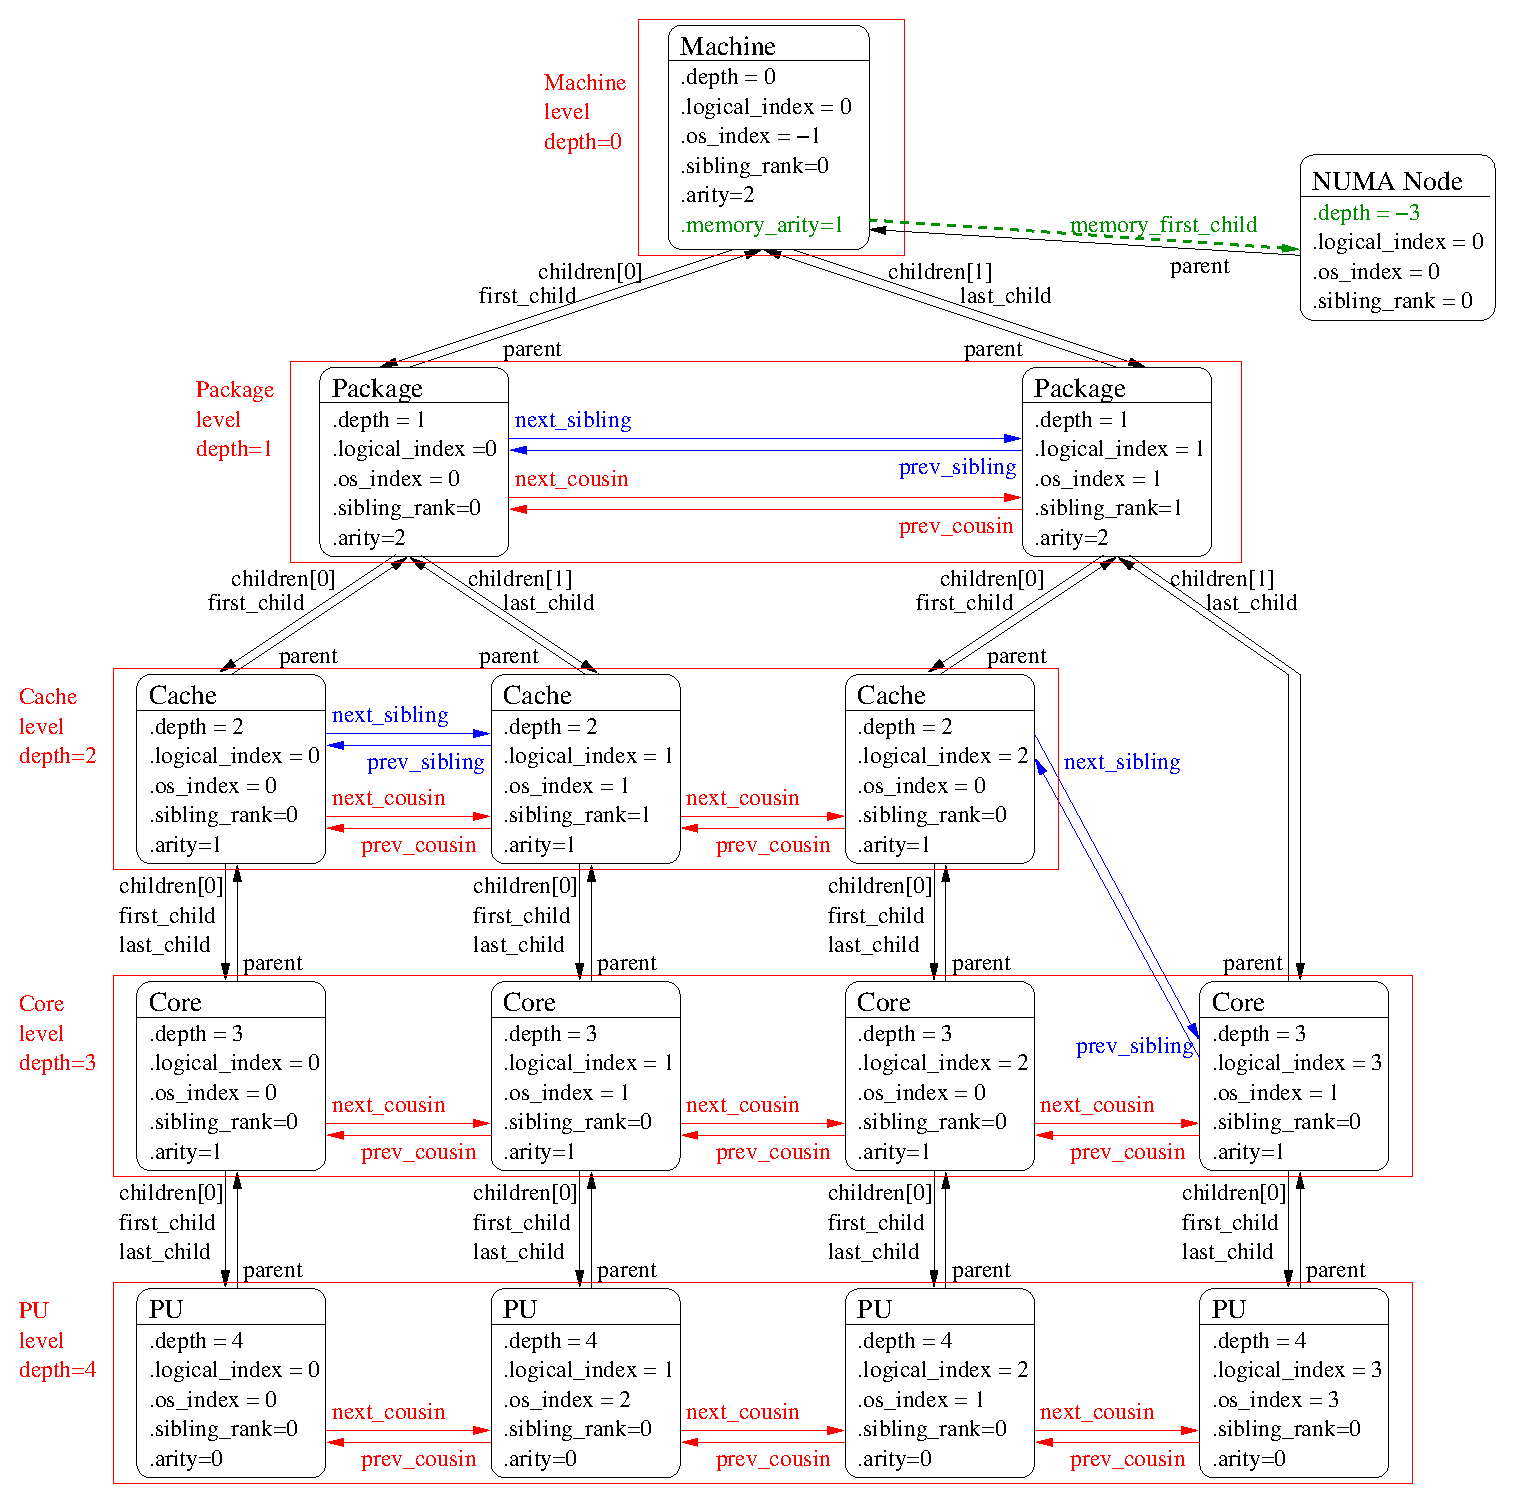
\includegraphics[width=\textwidth]{diagram}}
\end{DoxyImageNoCaption}


It should be noted that for PU objects, the logical index -- as computed linearly by hwloc -- is not the same as the OS index.

The N\+U\+MA node is on the side because it is not part of the main tree but rather attached to the object that corresponds to its locality (the entire machine here, hence the root object). It is attached as a {\itshape Memory} child (in green) and has a virtual depth (negative). It could also have siblings if there were multiple local N\+U\+MA nodes, or cousins if other N\+U\+MA nodes were attached somewhere else in the machine.

I/O or Misc objects could be attached in a similar manner. 
\chapter{Command-\/\+Line Tools}
\label{a00381}
\Hypertarget{a00381}


hwloc comes with an extensive C programming interface and several command line utilities. Each of them is fully documented in its own manual page; the following is a summary of the available command line tools.

 \hypertarget{a00381_cli_lstopo}{}\section{lstopo and lstopo-\/no-\/graphics}\label{a00381_cli_lstopo}
lstopo (also known as hwloc-\/ls) displays the hierarchical topology map of the current system. The output may be graphical, ascii-\/art or textual, and can also be exported to numerous file formats such as P\+DF, P\+NG, X\+ML, and others. Advanced graphical outputs require the \char`\"{}\+Cairo\char`\"{} development package (usually {\ttfamily cairo-\/devel} or {\ttfamily libcairo2-\/dev}).

lstopo and lstopo-\/no-\/graphics accept the same command-\/line options. However, graphical outputs are only available in lstopo. Textual outputs (those that do not depend on heavy external libraries such as Cairo) are supported in both lstopo and lstopo-\/no-\/graphics.

This command can also display the processes currently bound to a part of the machine (via the {\ttfamily -\/-\/ps} option).

Note that lstopo can read X\+ML files and/or alternate chroot filesystems and display topological maps representing those systems (e.\+g., use lstopo to output an X\+ML file on one system, and then use lstopo to read in that X\+ML file and display it on a different system).

 \hypertarget{a00381_cli_hwloc_bind}{}\section{hwloc-\/bind}\label{a00381_cli_hwloc_bind}
hwloc-\/bind binds processes to specific hardware objects through a flexible syntax. A simple example is binding an executable to specific cores (or packages or bitmaps or ...). The hwloc-\/bind(1) man page provides much more detail on what is possible.

hwloc-\/bind can also be used to retrieve the current process\textquotesingle{} binding, or retrieve the last C\+P\+U(s) where a process ran, or operate on memory binding.

Just like hwloc-\/calc, the input locations given to hwloc-\/bind may be either objects or cpusets (bitmaps as reported by hwloc-\/calc or hwloc-\/distrib).

 \hypertarget{a00381_cli_hwloc_calc}{}\section{hwloc-\/calc}\label{a00381_cli_hwloc_calc}
hwloc-\/calc is hwloc\textquotesingle{}s Swiss Army Knife command-\/line tool for converting things. The input may be either objects or cpusets (bitmaps as reported by another hwloc-\/calc instance or by hwloc-\/distrib), that may be combined by addition, intersection or subtraction. The output kinds include\+: 
\begin{DoxyItemize}
\item a cpuset bitmap\+: This compact opaque representation of objects is useful for shell scripts etc. It may passed to hwloc command-\/line tools such as hwloc-\/calc or hwloc-\/bind, or to hwloc command-\/line options such as {\ttfamily lstopo -\/-\/restrict}. 
\item the amount of the equivalent hwloc objects from a specific type, or the list of their indexes. This is useful for iterating over all similar objects (for instance all cores) within a given part of a platform. 
\item a hierarchical description of objects, for instance a thread index within a core within a package. This gives a better view of the actual location of an object. 
\end{DoxyItemize}

Moreover, input and/or output may be use either physical/\+OS object indexes or as hwloc\textquotesingle{}s logical object indexes. It eases cooperation with external tools such as taskset or numactl by exporting hwloc specifications into list of processor or N\+U\+MA node physical indexes. See also \hyperlink{a00394_faq_indexes}{Should I use logical or physical/\+OS indexes? and how?}.

 \hypertarget{a00381_cli_hwloc_info}{}\section{hwloc-\/info}\label{a00381_cli_hwloc_info}
hwloc-\/info dumps information about the given objects, as well as all its specific attributes. It is intended to be used with tools such as grep for filtering certain attribute lines. When no object is specified, or when {\ttfamily -\/-\/topology} is passed, hwloc-\/info prints a summary of the topology. When {\ttfamily -\/-\/support} is passed, hwloc-\/info lists the supported features for the topology.

 \hypertarget{a00381_cli_hwloc_distrib}{}\section{hwloc-\/distrib}\label{a00381_cli_hwloc_distrib}
hwloc-\/distrib generates a set of cpuset bitmaps that are uniformly distributed across the machine for the given number of processes. These strings may be used with hwloc-\/bind to run processes to maximize their memory bandwidth by properly distributing them across the machine.

 \hypertarget{a00381_cli_hwloc_ps}{}\section{hwloc-\/ps}\label{a00381_cli_hwloc_ps}
hwloc-\/ps is a tool to display the bindings of processes that are currently running on the local machine. By default, hwloc-\/ps only lists processes that are bound; unbound process (and Linux kernel threads) are not displayed.

 \hypertarget{a00381_cli_hwloc_annotate}{}\section{hwloc-\/annotate}\label{a00381_cli_hwloc_annotate}
hwloc-\/annotate may modify object (and topology) attributes such as string information (see \hyperlink{a00386_attributes_info}{Custom string infos} for details) or Misc children objects. It may also add distances, memory attributes, etc. to the topology. It reads an input topology from a X\+ML file and outputs the annotated topology as another X\+ML file.

 \hypertarget{a00381_cli_hwloc_diffpatchcompress}{}\section{hwloc-\/diff, hwloc-\/patch and hwloc-\/compress-\/dir}\label{a00381_cli_hwloc_diffpatchcompress}
hwloc-\/diff computes the difference between two topologies and outputs it to another X\+ML file.

hwloc-\/patch reads such a difference file and applies to another topology.

hwloc-\/compress-\/dir compresses an entire directory of X\+ML files by using hwloc-\/diff to save the differences between topologies instead of entire topologies.

 \hypertarget{a00381_cli_hwloc_dump_hwdata}{}\section{hwloc-\/dump-\/hwdata}\label{a00381_cli_hwloc_dump_hwdata}
hwloc-\/dump-\/hwdata is a Linux and x86-\/specific tool that dumps (during boot, privileged) some topology and locality information from raw hardware files (S\+M\+B\+I\+OS and A\+C\+PI tables) to human-\/readable and world-\/accessible files that the hwloc library will later reuse.

Currently only used on Intel Xeon Phi processor platforms. See \hyperlink{a00394_faq_knl_dump}{Why do I need hwloc-\/dump-\/hwdata for memory on Intel Xeon Phi processor?}.

See {\ttfamily H\+W\+L\+O\+C\+\_\+\+D\+U\+M\+P\+E\+D\+\_\+\+H\+W\+D\+A\+T\+A\+\_\+\+D\+IR} in \hyperlink{a00382}{Environment Variables} for details about the location of dumped files.

 \hypertarget{a00381_cli_hwloc_gather}{}\section{hwloc-\/gather-\/topology and hwloc-\/gather-\/cpuid}\label{a00381_cli_hwloc_gather}
hwloc-\/gather-\/topology is a Linux-\/specific tool that saves the relevant topology files of the current machine into a tarball (and the corresponding lstopo outputs).

hwloc-\/gather-\/cpuid is a x86-\/specific tool that dumps the result of C\+P\+U\+ID instructions on the current machine into a directory.

The output of hwloc-\/gather-\/cpuid is included in the tarball saved by hwloc-\/gather-\/topology when running on Linux/x86.

These files may be used later (possibly offline) for simulating or debugging a machine without actually running on it. 
\chapter{Environment Variables}
\label{a00382}
\Hypertarget{a00382}


The behavior of the hwloc library and tools may be tuned thanks to the following environment variables.


\begin{DoxyDescription}
\item[H\+W\+L\+O\+C\+\_\+\+X\+M\+L\+F\+I\+LE=/path/to/file.xml ]enforces the discovery from the given X\+ML file as if \hyperlink{a00192_ga879439b7ee99407ee911b3ac64e9a25e}{hwloc\+\_\+topology\+\_\+set\+\_\+xml()} had been called. This file may have been generated earlier with lstopo file.\+xml. For convenience, this backend provides empty binding hooks which just return success. To have hwloc still actually call O\+S-\/specific hooks, H\+W\+L\+O\+C\+\_\+\+T\+H\+I\+S\+S\+Y\+S\+T\+EM should be set 1 in the environment too, to assert that the loaded file is really the underlying system. See also \hyperlink{a00388}{Importing and exporting topologies from/to X\+ML files}. 


\item[H\+W\+L\+O\+C\+\_\+\+S\+Y\+N\+T\+H\+E\+T\+IC=synthetic\+\_\+description ]enforces the discovery through a synthetic description string as if \hyperlink{a00192_ga4fab186bb6181a00bcf585825fddd38d}{hwloc\+\_\+topology\+\_\+set\+\_\+synthetic()} had been called. For convenience, this backend provides empty binding hooks which just return success. See also \hyperlink{a00389}{Synthetic topologies}. 


\item[H\+W\+L\+O\+C\+\_\+\+X\+M\+L\+\_\+\+V\+E\+R\+B\+O\+SE=1 ]
\item[H\+W\+L\+O\+C\+\_\+\+S\+Y\+N\+T\+H\+E\+T\+I\+C\+\_\+\+V\+E\+R\+B\+O\+SE=1 ]enables verbose messages in the X\+ML or synthetic topology backends. hwloc X\+ML backends (see \hyperlink{a00388}{Importing and exporting topologies from/to X\+ML files}) can emit some error messages to the error output stream. Enabling these verbose messages within hwloc can be useful for understanding failures to parse input X\+ML topologies. Similarly, enabling verbose messages in the synthetic topology backend can help understand why the description string is invalid. See also \hyperlink{a00389}{Synthetic topologies}. 


\item[H\+W\+L\+O\+C\+\_\+\+T\+H\+I\+S\+S\+Y\+S\+T\+EM=1 ]enforces the return value of \hyperlink{a00193_ga68ffdcfd9175cdf40709801092f18017}{hwloc\+\_\+topology\+\_\+is\+\_\+thissystem()}, as if \hyperlink{a00193_ggada025d3ec20b4b420f8038d23d6e7bdea6ecb6abc6a0bb75e81564f8bca85783b}{H\+W\+L\+O\+C\+\_\+\+T\+O\+P\+O\+L\+O\+G\+Y\+\_\+\+F\+L\+A\+G\+\_\+\+I\+S\+\_\+\+T\+H\+I\+S\+S\+Y\+S\+T\+EM} was set with \hyperlink{a00193_gaaeed4df656979e5f16befea9d29b814b}{hwloc\+\_\+topology\+\_\+set\+\_\+flags()}. It means that it makes hwloc assume that the selected backend provides the topology for the system on which we are running, even if it is not the O\+S-\/specific backend but the X\+ML backend for instance. This means making the binding functions actually call the O\+S-\/specific system calls and really do binding, while the X\+ML backend would otherwise provide empty hooks just returning success. This can be used for efficiency reasons to first detect the topology once, save it to a X\+ML file, and quickly reload it later through the X\+ML backend, but still having binding functions actually do bind. This also enables support for the variable H\+W\+L\+O\+C\+\_\+\+T\+H\+I\+S\+S\+Y\+S\+T\+E\+M\+\_\+\+A\+L\+L\+O\+W\+E\+D\+\_\+\+R\+E\+S\+O\+U\+R\+C\+ES. 


\item[H\+W\+L\+O\+C\+\_\+\+T\+H\+I\+S\+S\+Y\+S\+T\+E\+M\+\_\+\+A\+L\+L\+O\+W\+E\+D\+\_\+\+R\+E\+S\+O\+U\+R\+C\+ES=1 ]Get the set of allowed resources from the native operating system even if the topology was loaded from X\+ML or synthetic description, as if \hyperlink{a00193_ggada025d3ec20b4b420f8038d23d6e7bdea1b66bbd66e900e5c837f71defb32ad89}{H\+W\+L\+O\+C\+\_\+\+T\+O\+P\+O\+L\+O\+G\+Y\+\_\+\+F\+L\+A\+G\+\_\+\+T\+H\+I\+S\+S\+Y\+S\+T\+E\+M\+\_\+\+A\+L\+L\+O\+W\+E\+D\+\_\+\+R\+E\+S\+O\+U\+R\+C\+ES} was set with \hyperlink{a00193_gaaeed4df656979e5f16befea9d29b814b}{hwloc\+\_\+topology\+\_\+set\+\_\+flags()}. This variable requires the topology to match the current system (see the variable H\+W\+L\+O\+C\+\_\+\+T\+H\+I\+S\+S\+Y\+S\+T\+EM). This is useful when the topology is not loaded directly from the local machine (e.\+g. for performance reason) and it comes with all resources, but the running process is restricted to only a part of the machine (for instance because of Linux Cgroup/\+Cpuset). 


\item[H\+W\+L\+O\+C\+\_\+\+A\+L\+L\+OW=all ]Totally ignore administrative restrictions such as Linux Cgroups and consider all resources (P\+Us and N\+U\+MA nodes) as allowed. This is different from setting H\+W\+L\+O\+C\+\_\+\+T\+O\+P\+O\+L\+O\+G\+Y\+\_\+\+F\+L\+A\+G\+\_\+\+I\+N\+C\+L\+U\+D\+E\+\_\+\+D\+I\+S\+A\+L\+L\+O\+W\+ED which gathers all resources but marks the unavailable ones as disallowed. 


\item[H\+W\+L\+O\+C\+\_\+\+H\+I\+D\+E\+\_\+\+E\+R\+R\+O\+RS=0 ]enables or disables verbose reporting of errors. The hwloc library may issue warnings to the standard error stream when it detects a problem during topology discovery, for instance if the operating system (or user) gives contradictory topology information. Setting this environment variable to 1 removes the actual displaying of these error messages. 


\item[H\+W\+L\+O\+C\+\_\+\+U\+S\+E\+\_\+\+N\+U\+M\+A\+\_\+\+D\+I\+S\+T\+A\+N\+C\+ES=7 ]enables or disables the use of N\+U\+MA distances. N\+U\+MA distances and memory target/initiator information may be used to improve the locality of N\+U\+MA nodes, especially C\+P\+U-\/less nodes. Bits in the value of this environment variable enable different features\+: Bit 0 enables the gathering of N\+U\+MA distances from the operating system. Bit 1 further enables the use of N\+U\+MA distances to improve the locality of C\+P\+U-\/less nodes. Bit 2 enables the use of target/initiator information. 


\item[H\+W\+L\+O\+C\+\_\+\+G\+R\+O\+U\+P\+I\+NG=1 ]enables or disables objects grouping based on distances. By default, hwloc uses distance matrices between objects (either read from the OS or given by the user) to find groups of close objects. These groups are described by adding intermediate Group objects in the topology. Setting this environment variable to 0 will disable this grouping. This variable supersedes the obsolete H\+W\+L\+O\+C\+\_\+\+I\+G\+N\+O\+R\+E\+\_\+\+D\+I\+S\+T\+A\+N\+C\+ES variable. 


\item[H\+W\+L\+O\+C\+\_\+\+G\+R\+O\+U\+P\+I\+N\+G\+\_\+\+A\+C\+C\+U\+R\+A\+CY=0.\+05 ]relaxes distance comparison during grouping. By default, objects may be grouped if their distances form a minimal distance graph. When setting this variable to 0.\+02, and when \hyperlink{a00210_gga22428b6bab271411e3834e6b4ca22e37a5233ccf631c3bc53dd5c3e7a5d5c9b77}{H\+W\+L\+O\+C\+\_\+\+D\+I\+S\+T\+A\+N\+C\+E\+S\+\_\+\+A\+D\+D\+\_\+\+F\+L\+A\+G\+\_\+\+G\+R\+O\+U\+P\+\_\+\+I\+N\+A\+C\+C\+U\+R\+A\+TE} is given, these distances do not have to be strictly equal anymore, they may just be equal with a 2\% error. If set to {\ttfamily try} instead of a numerical value, hwloc will try to group with perfect accuracy (0, the default), then with 0.\+01, 0.\+02, 0.\+05 and finally 0.\+1. Numbers given in this environment variable should always use a dot as a decimal mark (for instance 0.\+01 instead of 0,01).


\item[H\+W\+L\+O\+C\+\_\+\+G\+R\+O\+U\+P\+I\+N\+G\+\_\+\+V\+E\+R\+B\+O\+SE=0 ]enables or disables some verbose messages during grouping. If this variable is set to 1, some debug messages will be displayed during distance-\/based grouping of objects even if debug was not specific at configure time. This is useful when trying to find an interesting distance grouping accuracy.


\item[H\+W\+L\+O\+C\+\_\+\+C\+P\+U\+K\+I\+N\+D\+S\+\_\+\+R\+A\+N\+K\+I\+NG=default ]change the ranking policy for C\+PU kinds. By default, the O\+S-\/provided efficiency is used for ranking. If not available, the frequency is used on A\+RM processors, or core type and frequency on other architectures. ~\newline
 This environment variable may be set to {\ttfamily coretype+frequency}, {\ttfamily coretype}, {\ttfamily frequency}, {\ttfamily frequency\+\_\+base}, {\ttfamily frequency\+\_\+max}, {\ttfamily forced\+\_\+efficiency}, {\ttfamily no\+\_\+forced\+\_\+efficiency}, {\ttfamily default}, or {\ttfamily none}. 


\item[H\+W\+L\+O\+C\+\_\+\+P\+C\+I\+\_\+\+L\+O\+C\+A\+L\+I\+TY=$<$domain/bus$>$ $<$cpuset$>$;... ]
\item[H\+W\+L\+O\+C\+\_\+\+P\+C\+I\+\_\+\+L\+O\+C\+A\+L\+I\+TY=/path/to/pci/locality/file ]changes the locality of I/O devices behing the specified P\+CI buses. If no I/O locality information is available or if the B\+I\+OS reports incorrect information, it is possible to move a I/O device tree (OS and/or P\+CI devices with optional bridges) near a custom set of processors. ~\newline
 Localities are given either inside the environment variable itself, or in the pointed file. They may be separated either by semi-\/colons or by line-\/breaks. ~\newline
 Each locality contains a domain/bus specification (in hexadecimal numbers as usual) followed by a whitespace and a cpuset\+: 
\begin{DoxyItemize}
\item {\ttfamily 0001 $<$cpuset$>$} specifies the locality of all buses in P\+CI domain 0000. 
\item {\ttfamily 0000\+:0f $<$cpuset$>$} specifies only P\+CI bus 0f in domain 0000. 
\item {\ttfamily 0002\+:04-\/0a $<$cpuset$>$} specifies a range of buses (from 04 to 0a) within domain 0002. 
\end{DoxyItemize}Domain/bus specifications should usually match entire hierarchies of buses behind a bridge (including primary, secondary and subordinate buses). For instance, if hostbridge 0000\+:00 is above other bridges/switches with buses 0000\+:01 to 0000\+:09, the variable should be H\+W\+L\+O\+C\+\_\+\+P\+C\+I\+\_\+\+L\+O\+C\+A\+L\+I\+TY=\char`\"{}0000\+:00-\/09 $<$cpuset$>$\char`\"{}. It supersedes the old H\+W\+L\+O\+C\+\_\+\+P\+C\+I\+\_\+0000\+\_\+00\+\_\+\+L\+O\+C\+A\+L\+C\+P\+US=$<$cpuset$>$ which only works when hostbridges exist in the topology. ~\newline
 If the variable is defined to empty or invalid, no forced P\+CI locality is applied but hwloc\textquotesingle{}s internal automatic locality quirks are disabled, which means the exact P\+CI locality reported by the platform is used. 


\item[H\+W\+L\+O\+C\+\_\+\+X86\+\_\+\+T\+O\+P\+O\+E\+X\+T\+\_\+\+N\+U\+M\+A\+N\+O\+D\+ES=0 ]use A\+MD topoext C\+P\+U\+ID leaf in the x86 backend to detect N\+U\+MA nodes. When using the x86 backend, setting this variable to 1 enables the building of N\+U\+MA nodes from A\+MD processor C\+P\+U\+ID instructions. However this strategy does not always reflect B\+I\+OS configuration such as N\+U\+MA interleaving. And node indexes may be different from those of the operating system. Hence this should only be used when OS backends are wrong and the user is sure that C\+P\+U\+ID returns correct N\+U\+MA information. 


\item[H\+W\+L\+O\+C\+\_\+\+K\+E\+E\+P\+\_\+\+N\+V\+I\+D\+I\+A\+\_\+\+G\+P\+U\+\_\+\+N\+U\+M\+A\+\_\+\+N\+O\+D\+ES=0 ]show or hide N\+U\+MA nodes that correspond to N\+V\+I\+D\+IA G\+PU memory. By default they are ignored to avoid interleaved memory being allocated on G\+PU by mistake. Setting this environment variable to 1 exposes these N\+U\+MA nodes. They may be recognized by the {\itshape G\+P\+U\+Memory} subtype. They also have a {\itshape P\+C\+I\+Bus\+ID} info attribute to identify the corresponding G\+PU. 


\item[H\+W\+L\+O\+C\+\_\+\+K\+N\+L\+\_\+\+M\+S\+C\+A\+C\+H\+E\+\_\+\+L3=0 ]Expose the K\+NL M\+C\+D\+R\+AM in cache mode as a Memory-\/side Cache instead of a L3. hwloc releases prior to 2.\+1 exposed the M\+C\+D\+R\+AM cache as a C\+P\+U-\/side L3 cache. Now that Memory-\/side caches are supported by hwloc, it is still exposed as a L3 by default to avoid breaking existing applications. Setting this environment variable to 1 will expose it as a proper Memory-\/side cache. 


\item[H\+W\+L\+O\+C\+\_\+\+A\+N\+N\+O\+T\+A\+T\+E\+\_\+\+G\+L\+O\+B\+A\+L\+\_\+\+C\+O\+M\+P\+O\+N\+E\+N\+TS=0 ]Allow components to annotate the topology even if they are usually excluded by global components by default. Setting this variable to 1 and also setting {\ttfamily H\+W\+L\+O\+C\+\_\+\+C\+O\+M\+P\+O\+N\+E\+N\+TS=xml,pci,stop} enables the addition of P\+CI vendor and model info attributes to a X\+ML topology that was generated without those names (if pciaccess was missing). 


\item[H\+W\+L\+O\+C\+\_\+\+F\+S\+R\+O\+OT=/path/to/linux/filesystem-\/root/ ]switches to reading the topology from the specified Linux filesystem root instead of the main file-\/system root. This directory may have been saved previously from another machine with {\ttfamily hwloc-\/gather-\/topology}. ~\newline
 One should likely also set {\ttfamily H\+W\+L\+O\+C\+\_\+\+C\+O\+M\+P\+O\+N\+E\+N\+TS=linux,stop} so that non-\/\+Linux backends are disabled (the {\ttfamily -\/i} option of command-\/line tools takes care of both). ~\newline
 Not using the main file-\/system root causes \hyperlink{a00193_ga68ffdcfd9175cdf40709801092f18017}{hwloc\+\_\+topology\+\_\+is\+\_\+thissystem()} to return 0. For convenience, this backend provides empty binding hooks which just return success. To have hwloc still actually call O\+S-\/specific hooks, H\+W\+L\+O\+C\+\_\+\+T\+H\+I\+S\+S\+Y\+S\+T\+EM should be set 1 in the environment too, to assert that the loaded file is really the underlying system. 


\item[H\+W\+L\+O\+C\+\_\+\+C\+P\+U\+I\+D\+\_\+\+P\+A\+TH=/path/to/cpuid/ ]forces the x86 backend to read dumped C\+P\+U\+I\+Ds from the given directory instead of executing actual x86 C\+P\+U\+ID instructions. This directory may have been saved previously from another machine with {\ttfamily hwloc-\/gather-\/cpuid}. ~\newline
 One should likely also set {\ttfamily H\+W\+L\+O\+C\+\_\+\+C\+O\+M\+P\+O\+N\+E\+N\+TS=x86,stop} so that non-\/x86 backends are disabled (the {\ttfamily -\/i} option of command-\/line tools takes care of both). ~\newline
 It causes \hyperlink{a00193_ga68ffdcfd9175cdf40709801092f18017}{hwloc\+\_\+topology\+\_\+is\+\_\+thissystem()} to return 0. For convenience, this backend provides empty binding hooks which just return success. To have hwloc still actually call O\+S-\/specific hooks, H\+W\+L\+O\+C\+\_\+\+T\+H\+I\+S\+S\+Y\+S\+T\+EM should be set 1 in the environment too, to assert that the loaded C\+P\+U\+ID dump is really the underlying system. 


\item[H\+W\+L\+O\+C\+\_\+\+D\+U\+M\+P\+E\+D\+\_\+\+H\+W\+D\+A\+T\+A\+\_\+\+D\+IR=/path/to/dumped/files/ ]loads files dumped by {\ttfamily hwloc-\/dump-\/hwdata} (on Linux) from the given directory. The default dump/load directory is configured during build based on -\/-\/runstatedir, -\/-\/localstatedir, and -\/-\/prefix options. It usually points to {\ttfamily /var/run/hwloc/} in Linux distribution packages, but it may also point to {\ttfamily \$prefix/var/run/hwloc/} when manually installing and only specifying -\/-\/prefix. 


\item[H\+W\+L\+O\+C\+\_\+\+C\+O\+M\+P\+O\+N\+E\+N\+TS=list,of,components ]forces a list of components to enable or disable. Enable or disable the given comma-\/separated list of components (if they do not conflict with each other). Component names prefixed with {\ttfamily -\/} are disabled (a single phase may also be disabled).

Once the end of the list is reached, hwloc falls back to enabling the remaining components (sorted by priority) that do not conflict with the already enabled ones, and unless explicitly disabled in the list. If {\ttfamily stop} is met, the enabling loop immediately stops, no more component is enabled.

If {\ttfamily xml} or {\ttfamily synthetic} components are selected, the corresponding X\+ML filename or synthetic description string should be pass in {\ttfamily H\+W\+L\+O\+C\+\_\+\+X\+M\+L\+F\+I\+LE} or {\ttfamily H\+W\+L\+O\+C\+\_\+\+S\+Y\+N\+T\+H\+E\+T\+IC} respectively.

Since this variable is the low-\/level and more generic way to select components, it takes precedence over environment variables for selecting components.

If the variable is set to an empty string (or set to a single comma), no specific component is loaded first, all components are loaded in priority order.

See \hyperlink{a00392_plugins_select}{Selecting which components to use} for details. 


\item[H\+W\+L\+O\+C\+\_\+\+C\+O\+M\+P\+O\+N\+E\+N\+T\+S\+\_\+\+V\+E\+R\+B\+O\+SE=1 ]displays verbose information about components. Display messages when components are registered or enabled. This is the recommended way to list the available components with their priority (all of them are {\itshape registered} at startup). 


\item[H\+W\+L\+O\+C\+\_\+\+P\+L\+U\+G\+I\+N\+S\+\_\+\+P\+A\+TH=/path/to/hwloc/plugins/\+:... ]changes the default search directory for plugins. By default, {\ttfamily \$libdir/hwloc} is used. The variable may contain several colon-\/separated directories. 


\item[H\+W\+L\+O\+C\+\_\+\+P\+L\+U\+G\+I\+N\+S\+\_\+\+V\+E\+R\+B\+O\+SE=1 ]displays verbose information about plugins. List which directories are scanned, which files are loaded, and which components are successfully loaded. 


\item[H\+W\+L\+O\+C\+\_\+\+P\+L\+U\+G\+I\+N\+S\+\_\+\+B\+L\+A\+C\+K\+L\+I\+ST=filename1,filename2,... ]prevents plugins from being loaded if their filename (without path) is listed. Plugin filenames may be found in verbose messages outputted when H\+W\+L\+O\+C\+\_\+\+P\+L\+U\+G\+I\+N\+S\+\_\+\+V\+E\+R\+B\+O\+SE=1. 


\item[H\+W\+L\+O\+C\+\_\+\+D\+E\+B\+U\+G\+\_\+\+V\+E\+R\+B\+O\+SE=0 ]disables all verbose messages that are enabled by default when {\ttfamily --enable-\/debug} is passed to configure. When set to more than 1, even more verbose messages are displayed. The default is 1. 


\end{DoxyDescription}
\chapter{C\+PU and Memory Binding Overview}
\label{a00383}
\Hypertarget{a00383}


Some operating systems do not systematically provide separate functions for C\+PU and memory binding. This means that C\+PU binding functions may have have effects on the memory binding policy. Likewise, changing the memory binding policy may change the C\+PU binding of the current thread. This is often not a problem for applications, so by default hwloc will make use of these functions when they provide better binding support.

If the application does not want the C\+PU binding to change when changing the memory policy, it needs to use the \hyperlink{a00191_ggab00475fd98815bf4fb9aaf752030e7d2aad6b9eaf2ee324ca58dc8f58094b9997}{H\+W\+L\+O\+C\+\_\+\+M\+E\+M\+B\+I\+N\+D\+\_\+\+N\+O\+C\+P\+U\+B\+I\+ND} flag to prevent hwloc from using OS functions which would change the C\+PU binding. Additionally, \hyperlink{a00190_gga217dc8d373f8958cc93c154ebce1c71ca41ce440443cc3087caed95ab60edcad6}{H\+W\+L\+O\+C\+\_\+\+C\+P\+U\+B\+I\+N\+D\+\_\+\+N\+O\+M\+E\+M\+B\+I\+ND} can be passed to C\+PU binding function to prevent hwloc from using OS functions would change the memory binding policy. Of course, using these flags will reduce hwloc\textquotesingle{}s overall support for binding, so their use is discouraged.

One can avoid using these flags but still closely control both memory and C\+PU binding by allocating memory, touching each page in the allocated memory, and then changing the C\+PU binding. The already-\/really-\/allocated memory will then be \char`\"{}locked\char`\"{} to physical memory and will not be migrated. Thus, even if the memory binding policy gets changed by the C\+PU binding order, the already-\/allocated memory will not change with it. When binding and allocating further memory, the C\+PU binding should be performed again in case the memory binding altered the previously-\/selected C\+PU binding.

Not all operating systems support the notion of a \char`\"{}current\char`\"{} memory binding policy for the current process, but such operating systems often still provide a way to allocate data on a given node set. Conversely, some operating systems support the notion of a \char`\"{}current\char`\"{} memory binding policy and do not permit allocating data on a specific node set without changing the current policy and allocate the data. To provide the most powerful coverage of these facilities, hwloc provides\+:


\begin{DoxyItemize}
\item functions that set/get the current memory binding policies (if supported)\+: hwloc\+\_\+set/get\+\_\+membind() and hwloc\+\_\+set/get\+\_\+proc\+\_\+membind() 
\item a function that allocates memory bound to specific node set without changing the current memory binding policy (if supported)\+: \hyperlink{a00191_ga04736461780fadcf193af218c0122273}{hwloc\+\_\+alloc\+\_\+membind()}. 
\item a helper which, if needed, changes the current memory binding policy of the process in order to obtain memory binding\+: \hyperlink{a00191_gab1b77b8408bacaf03c7e8878f7577922}{hwloc\+\_\+alloc\+\_\+membind\+\_\+policy()}. 
\end{DoxyItemize}

An application can thus use the two first sets of functions if it wants to manage separately the global process binding policy and directed allocation, or use the third set of functions if it does not care about the process memory binding policy.

See \hyperlink{a00190}{C\+PU binding} and \hyperlink{a00191}{Memory binding} for hwloc\textquotesingle{}s A\+PI functions regarding C\+PU and memory binding, respectively. There are some examples under doc/examples/ in the source tree. 
\chapter{I/O Devices}
\label{a00384}
\Hypertarget{a00384}


hwloc usually manipulates processing units and memory but it can also discover I/O devices and report their locality as well. This is useful for placing I/O intensive applications on cores near the I/O devices they use, or for gathering information about all platform components.

 \hypertarget{a00384_iodevices_enabling}{}\section{Enabling and requirements}\label{a00384_iodevices_enabling}
I/O discovery is disabled by default (except in lstopo) for performance reasons. It can be enabled by changing the filtering of I/O object types to {\ttfamily \hyperlink{a00193_gga9a5a1f0140cd1952544477833733195ba63fd24954e18c83ff7eae9588759adb5}{H\+W\+L\+O\+C\+\_\+\+T\+Y\+P\+E\+\_\+\+F\+I\+L\+T\+E\+R\+\_\+\+K\+E\+E\+P\+\_\+\+I\+M\+P\+O\+R\+T\+A\+NT}} or {\ttfamily \hyperlink{a00193_gga9a5a1f0140cd1952544477833733195bafda7b59e6810dfe778d8f9a4cc1e350e}{H\+W\+L\+O\+C\+\_\+\+T\+Y\+P\+E\+\_\+\+F\+I\+L\+T\+E\+R\+\_\+\+K\+E\+E\+P\+\_\+\+A\+LL}} before loading the topology, for instance with {\ttfamily \hyperlink{a00193_ga0ab38705357bc1203abe829da8a12ad3}{hwloc\+\_\+topology\+\_\+set\+\_\+io\+\_\+types\+\_\+filter()}}.

Note that I/O discovery requires significant help from the operating system. The pciaccess library (the development package is usually {\ttfamily libpciaccess-\/devel} or {\ttfamily libpciaccess-\/dev}) is needed to fully detect P\+CI devices and bridges/switches. On Linux, P\+CI discovery may still be performed even if {\ttfamily libpciaccess} cannot be used. But it misses P\+CI device names. Moreover, some operating systems require privileges for probing P\+CI devices, see \hyperlink{a00394_faq_privileged}{Does hwloc require privileged access?} for details.

The actual locality of I/O devices is only currently detected on Linux. Other operating system will just report I/O devices as being attached to the topology root object.

 \hypertarget{a00384_iodevices_objects}{}\section{I/\+O objects}\label{a00384_iodevices_objects}
When I/O discovery is enabled and supported, some additional objects are added to the topology. The corresponding I/O object types are\+: 
\begin{DoxyItemize}
\item {\ttfamily \hyperlink{a00184_ggacd37bb612667dc437d66bfb175a8dc55a51e7280240fd9f25589cbbe538bdb075}{H\+W\+L\+O\+C\+\_\+\+O\+B\+J\+\_\+\+O\+S\+\_\+\+D\+E\+V\+I\+CE}} describes an operating-\/system-\/specific handle such as the {\itshape sda} drive or the {\itshape eth0} network interface. See \hyperlink{a00384_iodevices_osdev}{OS devices}. 
\item {\ttfamily \hyperlink{a00184_ggacd37bb612667dc437d66bfb175a8dc55a5d8117a54df1fbd3606ab19e42cb0ea9}{H\+W\+L\+O\+C\+\_\+\+O\+B\+J\+\_\+\+P\+C\+I\+\_\+\+D\+E\+V\+I\+CE}} and {\ttfamily \hyperlink{a00184_ggacd37bb612667dc437d66bfb175a8dc55a6825f10895fea60aca7a6ba9fe273db0}{H\+W\+L\+O\+C\+\_\+\+O\+B\+J\+\_\+\+B\+R\+I\+D\+GE}} build up a P\+CI hierarchy made of bridges (that may be actually be switches) and devices. See \hyperlink{a00384_iodevices_pci}{P\+CI devices and bridges}. 
\end{DoxyItemize}Any of these types may be filtered individually with {\ttfamily \hyperlink{a00193_gad894e70f15f8d4aada7be8d1aba38b7e}{hwloc\+\_\+topology\+\_\+set\+\_\+type\+\_\+filter()}}.

hwloc tries to attach these new objects to normal objects (usually N\+U\+MA nodes) to match their actual physical location. For instance, if a I/O hub (or root complex) is physically connected to a package, the corresponding hwloc bridge object (and its P\+CI bridges and devices children) is inserted as a child of the corresponding hwloc Package object. {\bfseries These children are not in the normal children list but rather in the I/\+O-\/specific children list.}

I/O objects also have neither C\+PU sets nor node sets (N\+U\+LL pointers) because they are not directly usable by the user applications for binding. Moreover I/O hierarchies may be highly complex (asymmetric trees of bridges). So I/O objects are placed in specific levels with custom depths. Their lists may still be traversed with regular helpers such as \hyperlink{a00187_ga759e88eaf5a230ad283e9d4c42486735}{hwloc\+\_\+get\+\_\+next\+\_\+obj\+\_\+by\+\_\+type()}. However, hwloc offers some dedicated helpers such as \hyperlink{a00204_ga66470dabce9db19a57c5940a909d0baa}{hwloc\+\_\+get\+\_\+next\+\_\+pcidev()} and \hyperlink{a00204_ga8b4584c8949e2c5f1c97ba7fe92b8145}{hwloc\+\_\+get\+\_\+next\+\_\+osdev()} for convenience (see \hyperlink{a00204}{Finding I/O objects}).

 \hypertarget{a00384_iodevices_osdev}{}\section{O\+S devices}\label{a00384_iodevices_osdev}
Although each P\+CI device is uniquely identified by its bus ID (e.\+g. 0000\+:01\+:02.\+3), a user-\/space application can hardly find out which P\+CI device it is actually using. Applications rather use software handles (such as the {\itshape eth0} network interface, the {\itshape sda} hard drive, or the {\itshape mlx4\+\_\+0} Open\+Fabrics H\+CA). Therefore hwloc tries to add software devices ({\ttfamily \hyperlink{a00184_ggacd37bb612667dc437d66bfb175a8dc55a51e7280240fd9f25589cbbe538bdb075}{H\+W\+L\+O\+C\+\_\+\+O\+B\+J\+\_\+\+O\+S\+\_\+\+D\+E\+V\+I\+CE}}, also known as OS devices).

OS devices may be attached below P\+CI devices, but they may also be attached directly to normal objects. Indeed some OS devices are not related to P\+CI. For instance, N\+V\+D\+I\+MM block devices (such as {\itshape pmem0s} on Linux) are directly attached near their N\+U\+MA node (I/O child of the parent whose memory child is the N\+U\+MA node). Also, if hwloc could not discover P\+CI for some reason, P\+C\+I-\/related OS devices may also be attached directly to normal objects.

hwloc first tries to discover OS devices from the operating system, e.\+g. {\itshape eth0}, {\itshape sda} or {\itshape mlx4\+\_\+0}. However, this ability is currently only available on Linux for some classes of devices.

hwloc then tries to discover software devices through additional I/O components using external libraries. For instance proprietary graphics drivers do not expose any named OS device, but hwloc may still create one OS object per software handle when supported. For instance the {\ttfamily opencl} and {\ttfamily cuda} components may add some {\itshape opencl0d0} and {\itshape cuda0} OS device objects.

Here is a list of OS device objects commonly created by hwloc components when I/O discovery is enabled and supported.


\begin{DoxyItemize}
\item Hard disks or non-\/volatile memory devices (\hyperlink{a00184_gga64f5d539df299c97ae80ce53fc4b56c0a689b0488c3c0d08d116751c6b9cb8871}{H\+W\+L\+O\+C\+\_\+\+O\+B\+J\+\_\+\+O\+S\+D\+E\+V\+\_\+\+B\+L\+O\+CK}) 
\begin{DoxyItemize}
\item {\itshape sda} or {\itshape dax2.\+0} (Linux component) 
\end{DoxyItemize}
\item Network interfaces (\hyperlink{a00184_gga64f5d539df299c97ae80ce53fc4b56c0ab715d81155f771573c8682dffc65021b}{H\+W\+L\+O\+C\+\_\+\+O\+B\+J\+\_\+\+O\+S\+D\+E\+V\+\_\+\+N\+E\+T\+W\+O\+RK}) 
\begin{DoxyItemize}
\item {\itshape eth0}, {\itshape wlan0}, {\itshape ib0} (Linux component) 
\end{DoxyItemize}
\item Open\+Fabrics (Infini\+Band, Omni-\/\+Path, us\+N\+IC, etc) H\+C\+As (\hyperlink{a00184_gga64f5d539df299c97ae80ce53fc4b56c0a52157d03694fdae82dddd57ca8c973b6}{H\+W\+L\+O\+C\+\_\+\+O\+B\+J\+\_\+\+O\+S\+D\+E\+V\+\_\+\+O\+P\+E\+N\+F\+A\+B\+R\+I\+CS}) 
\begin{DoxyItemize}
\item {\itshape mlx5\+\_\+0}, {\itshape hfi1\+\_\+0}, {\itshape qib0}, {\itshape usnic\+\_\+0} (Linux component) 
\end{DoxyItemize}
\item G\+P\+Us (\hyperlink{a00184_gga64f5d539df299c97ae80ce53fc4b56c0aa3a09798ef2836abb236dc3a645ffc90}{H\+W\+L\+O\+C\+\_\+\+O\+B\+J\+\_\+\+O\+S\+D\+E\+V\+\_\+\+G\+PU}) 
\begin{DoxyItemize}
\item {\itshape rsmi0} for the first R\+S\+MI device (R\+S\+MI component, using the A\+MD R\+O\+Cm S\+MI library) 
\item {\itshape nvml0} for the first N\+V\+ML device (N\+V\+ML component, using the N\+V\+I\+D\+IA Management Library) 
\item {\itshape \+:0.\+0} for the first display (GL component, using the N\+V-\/\+C\+O\+N\+T\+R\+OL X extension library, N\+V\+Ctrl) 
\end{DoxyItemize}
\item Co-\/\+Processors (\hyperlink{a00184_gga64f5d539df299c97ae80ce53fc4b56c0a46f8927e1c3e137eaa86cc8f6861fb83}{H\+W\+L\+O\+C\+\_\+\+O\+B\+J\+\_\+\+O\+S\+D\+E\+V\+\_\+\+C\+O\+P\+R\+OC}) 
\begin{DoxyItemize}
\item {\itshape opencl0d0} for the first device of the first Open\+CL platform, {\itshape opencl1d3} for the fourth device of the second Open\+CL platform (Open\+CL component) 
\item {\itshape cuda0} for the first N\+V\+I\+D\+IA C\+U\+DA device (C\+U\+DA component, using the N\+V\+I\+D\+IA C\+U\+DA Library)  
\item D\+MA engine channel (\hyperlink{a00184_gga64f5d539df299c97ae80ce53fc4b56c0a827ad1643360711a8b6c6af671366791}{H\+W\+L\+O\+C\+\_\+\+O\+B\+J\+\_\+\+O\+S\+D\+E\+V\+\_\+\+D\+MA}) 
\begin{DoxyItemize}
\item {\itshape dma0chan0} (Linux component) when all OS devices are enabled (\hyperlink{a00193_gga9a5a1f0140cd1952544477833733195bafda7b59e6810dfe778d8f9a4cc1e350e}{H\+W\+L\+O\+C\+\_\+\+T\+Y\+P\+E\+\_\+\+F\+I\+L\+T\+E\+R\+\_\+\+K\+E\+E\+P\+\_\+\+A\+LL}) 
\end{DoxyItemize}
\end{DoxyItemize}

Note that some P\+CI devices may contain multiple software devices (see the example below).

See also \hyperlink{a00390}{Interoperability With Other Software} for managing these devices without considering them as hwloc objects.

 
\end{DoxyItemize}\hypertarget{a00384_iodevices_pci}{}\section{P\+C\+I devices and bridges}\label{a00384_iodevices_pci}
A P\+CI hierarchy is usually organized as follows\+: A hostbridge object ( {\ttfamily \hyperlink{a00184_ggacd37bb612667dc437d66bfb175a8dc55a6825f10895fea60aca7a6ba9fe273db0}{H\+W\+L\+O\+C\+\_\+\+O\+B\+J\+\_\+\+B\+R\+I\+D\+GE}} object with upstream type {\itshape Host} and downstream type {\itshape P\+CI}) is attached below a normal object (usually the entire machine or a N\+U\+MA node). There may be multiple hostbridges in the machine, attached to different places, but all P\+CI devices are below one of them (unless the Bridge object type is filtered-\/out).

Each hostbridge contains one or several children, either other bridges (usually P\+CI to P\+CI switches) or P\+CI devices ({\ttfamily \hyperlink{a00184_ggacd37bb612667dc437d66bfb175a8dc55a5d8117a54df1fbd3606ab19e42cb0ea9}{H\+W\+L\+O\+C\+\_\+\+O\+B\+J\+\_\+\+P\+C\+I\+\_\+\+D\+E\+V\+I\+CE}}). The number of bridges between the hostbridge and a P\+CI device depends on the machine.

 \hypertarget{a00384_iodevices_consult}{}\section{Consulting I/\+O devices and binding}\label{a00384_iodevices_consult}
I/O devices may be consulted by traversing the topology manually (with usual routines such as \hyperlink{a00187_ga6f414dd80a2b943967a0ac92da3181a2}{hwloc\+\_\+get\+\_\+obj\+\_\+by\+\_\+type()}) or by using dedicated helpers (such as \hyperlink{a00204_gacdbaf0db98872e224b7883a84bfb0455}{hwloc\+\_\+get\+\_\+pcidev\+\_\+by\+\_\+busid()}, see \hyperlink{a00204}{Finding I/O objects}).

I/O objects do not actually contain any locality information because their C\+PU sets and node sets are N\+U\+LL. Their locality must be retrieved by walking up the object tree (through the {\ttfamily parent} link) until a non-\/\+I/O object is found (see \hyperlink{a00204_gaf139bb61375178e90cc3f1835b452ab6}{hwloc\+\_\+get\+\_\+non\+\_\+io\+\_\+ancestor\+\_\+obj()}). This normal object should have non-\/\+N\+U\+LL C\+PU sets and node sets which describe the processing units and memory that are immediately close to the I/O device. For instance the path from a OS device to its locality may go across a P\+CI device parent, one or several bridges, up to a Package node with the same locality.

Command-\/line tools are also aware of I/O devices. lstopo displays the interesting ones by default (passing {\ttfamily -\/-\/no-\/io} disables it).

hwloc-\/calc and hwloc-\/bind may manipulate I/O devices specified by P\+CI bus ID or by OS device name. 
\begin{DoxyItemize}
\item {\ttfamily pci=0000\+:02\+:03.\+0} is replaced by the set of C\+P\+Us that are close to the P\+CI device whose bus ID is given.  
\item {\ttfamily os=eth0} is replaced by C\+P\+Us that are close to the I/O device whose software handle is called {\ttfamily eth0}.  
\end{DoxyItemize}This enables easy binding of I/\+O-\/intensive applications near the device they use.

 \hypertarget{a00384_iodevices_examples}{}\section{Examples}\label{a00384_iodevices_examples}
The following picture shows a dual-\/package dual-\/core host whose P\+CI bus is connected to the first package and N\+U\+MA node.

 
\begin{DoxyImageNoCaption}
  \mbox{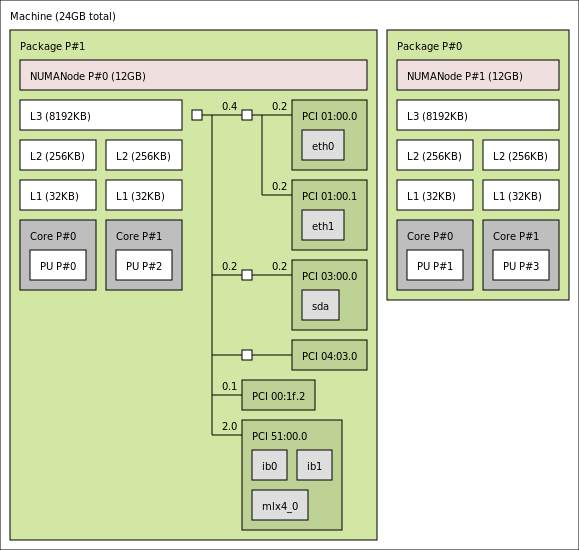
\includegraphics[width=\textwidth]{devel09-pci.png}}
\end{DoxyImageNoCaption}


Six interesting P\+CI devices were discovered. However, hwloc found some corresponding software devices ({\itshape eth0}, {\itshape eth1}, {\itshape sda}, {\itshape mlx4\+\_\+0}, {\itshape ib0}, and {\itshape ib1}) for only four of these physical devices. The other ones ({\itshape P\+CI 102b\+:0532} and {\itshape P\+CI 8086\+:3a20}) are an unused I\+DE controller (no disk attached) and a graphic card (no corresponding software device reported to the user by the operating system).

On the contrary, it should be noted that three different software devices were found for the last P\+CI device ({\itshape P\+CI 15b3\+:634a}). Indeed this Open\+Fabrics H\+CA P\+CI device object contains one one Open\+Fabrics software device ({\itshape mlx4\+\_\+0}) and two virtual network interface software devices ({\itshape ib0} and {\itshape ib1}).

Here is the corresponding textual output\+:

\begin{DoxyVerb}Machine (24GB total)
  Package L#0
    NUMANode L#0 (P#0 12GB)
    L3 L#0 (8192KB)
      L2 L#0 (256KB) + L1 L#0 (32KB) + Core L#0 + PU L#0 (P#0)
      L2 L#1 (256KB) + L1 L#1 (32KB) + Core L#1 + PU L#1 (P#2)
    HostBridge
      PCIBridge
        PCI 01:00.0 (Ethernet)
          Net "eth0"
        PCI 01:00.1 (Ethernet)
          Net "eth1"
      PCIBridge
        PCI 03:00.0 (RAID)
          Block "sda"
      PCIBridge
        PCI 04:03.0 (VGA)
      PCI 00:1f.2 (IDE)
      PCI 51:00.0 (InfiniBand)
        Net "ib0"
        Net "ib1"
        Net "mlx4_0"
  Package L#1
    NUMANode L#1 (P#1 12GB)
    L3 L#1 (8192KB)
      L2 L#2 (256KB) + L1 L#2 (32KB) + Core L#2 + PU L#2 (P#1)
      L2 L#3 (256KB) + L1 L#3 (32KB) + Core L#3 + PU L#3 (P#3)
\end{DoxyVerb}
 
\chapter{Miscellaneous objects}
\label{a00385}
\Hypertarget{a00385}


hwloc topologies may be annotated with Misc objects (of type {\ttfamily \hyperlink{a00184_ggacd37bb612667dc437d66bfb175a8dc55a19f8a6953fa91efc76bcbcdf2d22de4d}{H\+W\+L\+O\+C\+\_\+\+O\+B\+J\+\_\+\+M\+I\+SC}}) either automatically or by the user. This is a flexible way to annotate topologies with large sets of information since Misc objects may be inserted anywhere in the topology (to annotate specific objects or parts of the topology), even below other Misc objects, and each of them may contain multiple attributes (see also \hyperlink{a00394_faq_annotate}{How do I annotate the topology with private notes?}).

These Misc objects may have a {\ttfamily subtype} field to replace {\ttfamily Misc} with something else in the lstopo output.

 \hypertarget{a00385_miscobjs_auto}{}\section{Misc objects added by hwloc}\label{a00385_miscobjs_auto}
hwloc only uses Misc objects when other object types are not sufficient, and when the Misc object type is not filtered-\/out anymore. This currently includes\+: 
\begin{DoxyItemize}
\item Memory modules (D\+I\+M\+Ms), on Linux when privileged and when {\ttfamily dmi-\/sysfs} is supported by the kernel. These objects have a {\ttfamily subtype} field of value {\ttfamily Memory\+Module}. They are currently always attached to the root object. Their attributes describe the D\+I\+MM vendor, model, etc. {\ttfamily lstopo -\/v} displays them as\+: 
\begin{DoxyCode}
Misc(MemoryModule) (P#1 DeviceLocation=\textcolor{stringliteral}{"Bottom-Slot 2(right)"} BankLocation=\textcolor{stringliteral}{"BANK 2"} Vendor=Elpida 
      SerialNumber=21733667 AssetTag=9876543210 PartNumber=\textcolor{stringliteral}{"EBJ81UG8EFU0-GN-F "})
\end{DoxyCode}
  
\item Displaying process binding in {\ttfamily lstopo -\/-\/top}. These objects have a {\ttfamily subtype} field of value {\ttfamily Process} and a name attribute made of their P\+ID and program name. They are attached below the object they are bound to. The textual {\ttfamily lstopo} displays them as\+: 
\begin{DoxyCode}
PU L#0 (P#0)
  Misc(Process) 4445 myprogram
\end{DoxyCode}
  
\end{DoxyItemize}

 \hypertarget{a00385_miscobjs_annotate}{}\section{Annotating topologies with Misc objects}\label{a00385_miscobjs_annotate}
The user may annotate hwloc topologies with its own Misc objects. This can be achieved with {\ttfamily \hyperlink{a00194_gad980782ade737900c5cf208946768c30}{hwloc\+\_\+topology\+\_\+insert\+\_\+misc\+\_\+object()}} as well as hwloc-\/annotate command-\/line tool. 
\chapter{Object attributes}
\label{a00386}
\Hypertarget{a00386}
 \hypertarget{a00386_attributes_normal}{}\section{Normal attributes}\label{a00386_attributes_normal}
hwloc objects have many generic attributes in the \hyperlink{a00238}{hwloc\+\_\+obj} structure, for instance their {\ttfamily logical\+\_\+index} or {\ttfamily os\+\_\+index} (see \hyperlink{a00394_faq_indexes}{Should I use logical or physical/\+OS indexes? and how?}), {\ttfamily depth} or {\ttfamily name}.

The kind of object is first described by the {\ttfamily obj-\/$>$type} generic attribute (an integer). OS devices also have a specific {\ttfamily obj-\/$>$attr-\/$>$osdev.\+type} integer for distinguishing between N\+I\+Cs, G\+P\+Us, etc. Objects may also have an optional {\ttfamily obj-\/$>$subtype} pointing to a better description string. For instance subtype is useful to say what Group objects are actually made of (e.\+g. {\itshape Book} for Linux S/390 books). It may also specify that a Block OS device is a {\itshape Disk}, or that a Co\+Processor OS device is a {\itshape C\+U\+DA} device. This subtype is displayed by lstopo either in place or after the main {\ttfamily obj-\/$>$type} attribute. N\+U\+MA nodes that correspond G\+PU memory may also have {\itshape G\+P\+U\+Memory} as subtype.

Each object also contains an {\ttfamily attr} field that, if non N\+U\+LL, points to a union \hyperlink{a00242}{hwloc\+\_\+obj\+\_\+attr\+\_\+u} of type-\/specific attribute structures. For instance, a L2\+Cache object {\ttfamily obj} contains cache-\/specific information in {\ttfamily obj-\/$>$attr-\/$>$cache}, such as its size and associativity, cache type. See \hyperlink{a00242}{hwloc\+\_\+obj\+\_\+attr\+\_\+u} for details.

 \hypertarget{a00386_attributes_info}{}\section{Custom string infos}\label{a00386_attributes_info}
Aside os these generic attribute fields, hwloc annotates many objects with string attributes that are made of a key and a value. Each object contains a list of such pairs that may be consulted manually (looking at the object {\ttfamily infos} array field) or using the \hyperlink{a00189_gab358661a92bb27d8542b255cc9f6f25e}{hwloc\+\_\+obj\+\_\+get\+\_\+info\+\_\+by\+\_\+name()}. The user may additionally add new key-\/value pairs to any object using \hyperlink{a00189_gace7654bb8a9002caae1a4b8a59e7452e}{hwloc\+\_\+obj\+\_\+add\+\_\+info()} or the \hyperlink{a00381_cli_hwloc_annotate}{hwloc-\/annotate} program.

Here is a non-\/exhaustive list of attributes that may be automatically added by hwloc. Note that these attributes heavily depend on the ability of the operating system to report them. Many of them will therefore be missing on some OS.

 \hypertarget{a00386_attributes_info_platform}{}\subsection{Hardware Platform Information}\label{a00386_attributes_info_platform}
These info attributes are attached to the root object (Machine).


\begin{DoxyDescription}
\item[Platform\+Name, Platform\+Model, Platform\+Vendor, Platform\+Board\+ID, Platform\+Revision, ]
\item[System\+Version\+Register, Processor\+Version\+Register (Machine) ]Some P\+O\+W\+E\+R/\+Power\+P\+C-\/specific attributes describing the platform and processor. Currently only available on Linux. Usually added to Package objects, but can be in Machine instead if hwloc failed to discover any package.  
\item[D\+M\+I\+Board\+Vendor, D\+M\+I\+Board\+Name, etc. ]D\+MI hardware information such as the motherboard and chassis models and vendors, the B\+I\+OS revision, etc., as reported by Linux under {\ttfamily /sys/class/dmi/id/}.  
\item[Memory\+Mode, Cluster\+Mode ]Intel Xeon Phi processor configuration modes. Available if hwloc-\/dump-\/hwdata was used (see \hyperlink{a00394_faq_knl_dump}{Why do I need hwloc-\/dump-\/hwdata for memory on Intel Xeon Phi processor?}) or if hwloc managed to guess them from the N\+U\+MA configuration.

The memory mode may be {\itshape Cache}, {\itshape Flat}, {\itshape Hybrid50} (half the M\+C\+D\+R\+AM is used as a cache) or {\itshape Hybrid25} (25\% of M\+C\+D\+R\+AM as cache). The cluster mode may be {\itshape Quadrant}, {\itshape Hemisphere}, {\itshape All2\+All}, {\itshape S\+N\+C2} or {\itshape S\+N\+C4}. See doc/examples/get-\/knl-\/modes.\+c in the source directory for an example of retrieving these attributes.  
\end{DoxyDescription}

 \hypertarget{a00386_attributes_info_os}{}\subsection{Operating System Information}\label{a00386_attributes_info_os}
These info attributes are attached to the root object (Machine).


\begin{DoxyDescription}
\item[O\+S\+Name, O\+S\+Release, O\+S\+Version, Host\+Name, Architecture ]The operating system name, release, version, the hostname and the architecture name, as reported by the Unix {\ttfamily uname} command.  
\item[Linux\+Cgroup ]The name the Linux control group where the calling process is placed.  
\item[Windows\+Build\+Environment ]Either Min\+GW or Cygwin when one of these environments was used during build.  
\end{DoxyDescription}

 \hypertarget{a00386_attributes_info_hwloc}{}\subsection{hwloc Information}\label{a00386_attributes_info_hwloc}
Unless specified, these info attributes are attached to the root object (Machine).


\begin{DoxyDescription}
\item[Backend (topology root, or specific object added by that backend) ]The name of the hwloc backend/component that filled the topology. If several components were combined, multiple Backend keys may exist, with different values, for instance {\ttfamily x86} and {\ttfamily Linux} in the root object and {\ttfamily C\+U\+DA} in C\+U\+DA OS device objects.  
\item[Synthetic\+Description ]The description string that was given to hwloc to build this synthetic topology.  
\item[hwloc\+Version ]The version number of the hwloc library that was used to generate the topology. If the topology was loaded from X\+ML, this is not the hwloc version that loaded it, but rather the first hwloc instance that exported the topology to X\+ML earlier.  
\item[Process\+Name ]The name of the process that contains the hwloc library that was used to generate the topology. If the topology was from X\+ML, this is not the hwloc process that loaded it, but rather the first process that exported the topology to X\+ML earlier.  
\end{DoxyDescription}

 \hypertarget{a00386_attributes_info_cpu}{}\subsection{C\+P\+U Information}\label{a00386_attributes_info_cpu}
These info attributes are attached to Package objects, or to the root object (Machine) if package locality information is missing.


\begin{DoxyDescription}
\item[C\+P\+U\+Model ]The processor model name. 
\item[C\+P\+U\+Vendor, C\+P\+U\+Model\+Number, C\+P\+U\+Family\+Number, C\+P\+U\+Stepping ]The processor vendor name, model number, family number, and stepping number. Currently available for x86 and Xeon Phi processors on most systems, and for ia64 processors on Linux (except C\+P\+U\+Stepping).  
\item[C\+P\+U\+Revision ]A P\+O\+W\+E\+R/\+Power\+P\+C-\/specific general processor revision number, currently only available on Linux.  
\item[C\+P\+U\+Type ]A Solaris-\/specific general processor type name, such as \char`\"{}i86pc\char`\"{}.  
\end{DoxyDescription}

 \hypertarget{a00386_attributes_info_osdev}{}\subsection{O\+S Device Information}\label{a00386_attributes_info_osdev}
These info attributes are attached to OS device objects specified in parentheses.


\begin{DoxyDescription}
\item[Vendor, Model, Revision, Serial\+Number, Size, Sector\+Size (Block OS devices) ]The vendor and model names, revision, serial number, size (in kB) and Sector\+Size (in bytes).  
\item[Linux\+Device\+ID (Block OS devices) ]The major/minor device number such as 8\+:0 of Linux device.  
\item[G\+P\+U\+Vendor, G\+P\+U\+Model (G\+PU or Co-\/\+Processor OS devices) ]The vendor and model names of the G\+PU device.  
\item[Open\+C\+L\+Device\+Type, Open\+C\+L\+Platform\+Index, ]
\item[Open\+C\+L\+Platform\+Name, Open\+C\+L\+Platform\+Device\+Index (Open\+CL OS devices) ]The type of Open\+CL device, the Open\+CL platform index and name, and the index of the device within the platform.  
\item[Open\+C\+L\+Compute\+Units, Open\+C\+L\+Global\+Memory\+Size (Open\+CL OS devices) ]The number of compute units and global memory size (in kB) of an Open\+CL device.  
\item[A\+M\+D\+U\+U\+ID, A\+M\+D\+Serial (R\+S\+MI G\+PU OS devices) ]The U\+U\+ID and serial number of A\+MD G\+P\+Us.  
\item[X\+G\+M\+I\+Hive\+ID (R\+S\+MI G\+PU OS devices) ]The ID of the group of G\+P\+Us (Hive) interconnected by X\+G\+MI links  
\item[X\+G\+M\+I\+Peers (R\+S\+MI G\+PU OS devices) ]The list of R\+S\+MI OS devices that are directly connected to the current device through X\+G\+MI links. They are given as a space-\/separated list of object names, for instance {\itshape rsmi2 rsmi3}.  
\item[N\+V\+I\+D\+I\+A\+U\+U\+ID, N\+V\+I\+D\+I\+A\+Serial (N\+V\+ML G\+PU OS devices) ]The U\+U\+ID and serial number of N\+V\+I\+D\+IA G\+P\+Us.  
\item[C\+U\+D\+A\+Multi\+Processors, C\+U\+D\+A\+Cores\+Per\+MP, ]
\item[C\+U\+D\+A\+Global\+Memory\+Size, C\+U\+D\+A\+L2\+Cache\+Size, C\+U\+D\+A\+Shared\+Memory\+Size\+Per\+MP (C\+U\+DA OS devices) ]The number of shared multiprocessors, the number of cores per multiprocessor, the global memory size, the (global) L2 cache size, and size of the shared memory in each multiprocessor of a C\+U\+DA device. Sizes are in kB.  
\item[Address, Port (Network interface OS devices) ]The M\+AC address and the port number of a software network interface, such as {\ttfamily eth4} on Linux.  
\item[Node\+G\+U\+ID, Sys\+Image\+G\+U\+ID, Port1\+State, Port2\+L\+ID, Port2\+L\+MC, Port3\+G\+I\+D1 (Open\+Fabrics OS devices) ]The node G\+U\+ID and G\+U\+ID mask, the state of a port \#1 (value is 4 when active), the L\+ID and L\+ID mask count of port \#2, and G\+ID \#1 of port \#3.  
\end{DoxyDescription}

 \hypertarget{a00386_attributes_info_otherobjs}{}\subsection{Other Object-\/specific Information}\label{a00386_attributes_info_otherobjs}
These info attributes are attached to objects specified in parentheses.


\begin{DoxyDescription}
\item[D\+A\+X\+Device (N\+U\+MA Nodes) ]The name of the Linux D\+AX device that was used to expose a non-\/volatile memory region as a volatile N\+U\+MA node.  
\item[P\+C\+I\+Bus\+ID (G\+P\+U\+Memory N\+U\+MA Nodes) ]The P\+CI bus ID of the G\+PU whose memory is exposed in this N\+U\+MA node.  
\item[Inclusive (Caches) ]The inclusiveness of a cache (1 if inclusive, 0 otherwise). Currently only available on x86 processors.  
\item[Solaris\+Processor\+Group (Group) ]The Solaris kstat processor group name that was used to build this Group object.  
\item[P\+C\+I\+Vendor, P\+C\+I\+Device (P\+CI devices and bridges) ]The vendor and device names of the P\+CI device.  
\item[P\+C\+I\+Slot (P\+CI devices or Bridges) ]The name/number of the physical slot where the device is plugged. If the physical device contains P\+CI bridges above the actual P\+CI device, the attribute may be attached to the highest bridge (i.\+e. the first object that actually appears below the physical slot).  
\item[Vendor, Asset\+Tag, Part\+Number, Device\+Location, Bank\+Location (Memory\+Module Misc objects) ]Information about memory modules (D\+I\+M\+Ms) extracted from S\+M\+B\+I\+OS.  
\end{DoxyDescription}

 \hypertarget{a00386_attributes_info_user}{}\subsection{User-\/\+Given Information}\label{a00386_attributes_info_user}
Here is a non-\/exhaustive list of user-\/provided info attributes that have a special meaning\+: 
\begin{DoxyDescription}
\item[lstopo\+Style ]Enforces the style of an object (background and text colors) in the graphical output of lstopo. See C\+U\+S\+T\+OM C\+O\+L\+O\+RS in the lstopo(1) manpage for details.  
\end{DoxyDescription}
\chapter{Topology Attributes\+: Distances, Memory Attributes and C\+PU Kinds}
\label{a00387}
\Hypertarget{a00387}


Besides the hierarchy of objects and individual object attributes (see \hyperlink{a00386}{Object attributes}), hwloc may also expose finer information about the hardware organization.

 \hypertarget{a00387_topoattrs_distances}{}\section{Distances}\label{a00387_topoattrs_distances}
A machine with 4 C\+P\+Us may have identical links between every pairs of C\+P\+Us, or those C\+P\+Us could also only be connected through a ring. In the ring case, accessing the memory of nearby C\+P\+Us is slower than local memory, but it is also faster than accessing the memory of C\+PU on the opposite side of the ring. These deep details cannot be exposed in the hwloc hierarchy, that is why hwloc also exposes distances.

Distances are matrices of values between sets of objects, usually latencies or bandwidths. By default, hwloc tries to get a matrix of relative latencies between N\+U\+MA nodes when exposed by the hardware.

In the aforementioned ring case, the matrix could report 10 for latency between a N\+U\+MA node and itself, 20 for nearby nodes, and 30 for nodes that are opposites on the ring. Those are theoretical values exposed by hardware vendors (in the System Locality Distance Information Table (S\+L\+IT) in the A\+C\+PI) rather than physical latencies. They are mostly meant for comparing node relative distances.

Distances structures currently created by hwloc are\+: 
\begin{DoxyDescription}
\item[N\+U\+M\+A\+Latency (Linux, Solaris, Free\+B\+SD) ]This is the matrix of theoretical latencies described above.  
\end{DoxyDescription}

Users may also specify their own matrices between any set of objects, even if these objects are of different types (e.\+g. bandwidths between G\+P\+Us and C\+P\+Us).

The entire A\+PI is located in \hyperlink{a00131_source}{hwloc/distances.\+h}. See also \hyperlink{a00208}{Retrieve distances between objects}, as well as \hyperlink{a00209}{Helpers for consulting distance matrices} and \hyperlink{a00210}{Add or remove distances between objects}.

 \hypertarget{a00387_topoattrs_memattrs}{}\section{Memory Attributes}\label{a00387_topoattrs_memattrs}
Machines with heterogeneous memory, for instance high-\/bandwidth memory (H\+BM), normal memory (D\+DR), and/or high-\/capacity slow memory (such as non-\/volatile memory D\+I\+M\+Ms, N\+V\+D\+I\+M\+Ms) require applications to allocate buffers in the appropriate target memory depending on performance and capacity needs. Those target nodes may be exposed in the hwloc hierarchy as different memory children but there is a need for performance information to select the appropriate one.

hwloc memory attributes are designed to expose memory information such as latency, bandwidth, etc. Users may also specify their own attributes and values.

The memory attributes A\+PI is located in \hyperlink{a00134_source}{hwloc/memattrs.\+h}, see \hyperlink{a00211}{Comparing memory node attributes for finding where to allocate on} and \hyperlink{a00212}{Managing memory attributes} for details.

 \hypertarget{a00387_topoattrs_cpukinds}{}\section{C\+P\+U Kinds}\label{a00387_topoattrs_cpukinds}
Hybrid C\+P\+Us may contain different kinds of cores. The C\+PU kinds A\+PI in \hyperlink{a00137_source}{hwloc/cpukinds.\+h} provides a way to list the sets of P\+Us in each kind and get some optional information about their hardware characteristics and efficiency.

If the operating system provides efficiency information (e.\+g. Windows 10), it is used to rank hwloc C\+PU kinds by efficiency. Otherwise, hwloc implements several heuristics based on frequencies and core types (see H\+W\+L\+O\+C\+\_\+\+C\+P\+U\+K\+I\+N\+D\+S\+\_\+\+R\+A\+N\+K\+I\+NG in \hyperlink{a00382}{Environment Variables}).

Attributes include\+: 
\begin{DoxyDescription}
\item[Frequency\+Max\+M\+Hz (Linux) ]The maximal operating frequency of the core, as reported by {\ttfamily cpufreq} drivers on Linux.  
\item[Frequency\+Base\+M\+Hz (Linux) ]The base operating frequency of the core, as reported by some {\ttfamily cpufreq} drivers on Linux (e.\+g. {\ttfamily intel\+\_\+pstate}).  
\item[Core\+Type (x86, Linux) ]A string describing the kind of core, currently {\ttfamily Intel\+Atom} or {\ttfamily Intel\+Core}, as reported by the x86 C\+P\+U\+ID instruction and future Linux kernels on some Intel processors.  
\item[Linux\+C\+P\+U\+Type (Linux) ]The Linux-\/specific C\+PU type found in sysfs, such as {\ttfamily intel\+\_\+atom\+\_\+0}, as reported by future Linux kernels on some Intel processors.  
\end{DoxyDescription}

See \hyperlink{a00213}{Kinds of C\+PU cores} for details. 
\chapter{Importing and exporting topologies from/to X\+ML files}
\label{a00388}
\Hypertarget{a00388}


hwloc offers the ability to export topologies to X\+ML files and reload them later. This is for instance useful for loading topologies faster (see \hyperlink{a00394_faq_xml}{I do not want hwloc to rediscover my enormous machine topology every time I rerun a process}), manipulating other nodes\textquotesingle{} topology, or avoiding the need for privileged processes (see \hyperlink{a00394_faq_privileged}{Does hwloc require privileged access?}).

Topologies may be exported to X\+ML files thanks to \hyperlink{a00206_ga333f79975b4eeb28a3d8fad3373583ce}{hwloc\+\_\+topology\+\_\+export\+\_\+xml()}, or to a X\+ML memory buffer with \hyperlink{a00206_gad33b7f7c11db10459505a3b1634fd3f1}{hwloc\+\_\+topology\+\_\+export\+\_\+xmlbuffer()}. The lstopo program can also serve as a X\+ML topology export tool.

X\+ML topologies may then be reloaded later with \hyperlink{a00192_ga879439b7ee99407ee911b3ac64e9a25e}{hwloc\+\_\+topology\+\_\+set\+\_\+xml()} and \hyperlink{a00192_ga2745616b65595e1c1e579ecc7e461fa8}{hwloc\+\_\+topology\+\_\+set\+\_\+xmlbuffer()}. The H\+W\+L\+O\+C\+\_\+\+X\+M\+L\+F\+I\+LE environment variable also tells hwloc to load the topology from the given X\+ML file (see \hyperlink{a00382}{Environment Variables}).

\begin{DoxyNote}{Note}
Loading X\+ML topologies disables binding because the loaded topology may not correspond to the physical machine that loads it. This behavior may be reverted by asserting that loaded file really matches the underlying system with the H\+W\+L\+O\+C\+\_\+\+T\+H\+I\+S\+S\+Y\+S\+T\+EM environment variable or the \hyperlink{a00193_ggada025d3ec20b4b420f8038d23d6e7bdea6ecb6abc6a0bb75e81564f8bca85783b}{H\+W\+L\+O\+C\+\_\+\+T\+O\+P\+O\+L\+O\+G\+Y\+\_\+\+F\+L\+A\+G\+\_\+\+I\+S\+\_\+\+T\+H\+I\+S\+S\+Y\+S\+T\+EM} topology flag.

The topology flag \hyperlink{a00193_ggada025d3ec20b4b420f8038d23d6e7bdea1b66bbd66e900e5c837f71defb32ad89}{H\+W\+L\+O\+C\+\_\+\+T\+O\+P\+O\+L\+O\+G\+Y\+\_\+\+F\+L\+A\+G\+\_\+\+T\+H\+I\+S\+S\+Y\+S\+T\+E\+M\+\_\+\+A\+L\+L\+O\+W\+E\+D\+\_\+\+R\+E\+S\+O\+U\+R\+C\+ES} may be used to load a X\+ML topology that contains the entire machine and restrict it to the part that is actually available to the current process (e.\+g. when Linux Cgroup/\+Cpuset are used to restrict the set of resources).

hwloc also offers the ability to export/import \hyperlink{a00225}{Topology differences}.

X\+ML topology files are not localized. They use a dot as a decimal separator. Therefore any exported topology can be reloaded on any other machine without requiring to change the locale.

X\+ML exports contain all details about the platform. It means that two very similar nodes still have different X\+ML exports (e.\+g. some serial numbers or M\+AC addresses are different). If a less precise exporting/importing is required, one may want to look at \hyperlink{a00389}{Synthetic topologies} instead.
\end{DoxyNote}
 \hypertarget{a00388_xml_backends}{}\section{libxml2 and minimalistic X\+M\+L backends}\label{a00388_xml_backends}
hwloc offers two backends for importing/exporting X\+ML.

First, it can use the libxml2 library for importing/exporting X\+ML files. It features full X\+ML support, for instance when those files have to be manipulated by non-\/hwloc software (e.\+g. a X\+S\+LT parser). The libxml2 backend is enabled by default if libxml2 development headers are available (the relevant development package is usually {\ttfamily libxml2-\/devel} or {\ttfamily libxml2-\/dev}).

If libxml2 is not available at configure time, or if {\ttfamily -\/-\/disable-\/libxml2} is passed, hwloc falls back to a custom backend. Contrary to the aforementioned full X\+ML backend with libxml2, this minimalistic X\+ML backend cannot be guaranteed to work with external programs. It should only be assumed to be compatible with the same hwloc release (even if using the libxml2 backend). Its advantage is, however, to always be available without requiring any external dependency.

If libxml2 is available but the core hwloc library should not directly depend on it, the libxml2 support may be built as a dynamicall-\/loaded plugin. One should pass {\ttfamily -\/-\/enable-\/plugins} to enable plugin support (when supported) and build as plugins all component that support it. Or pass {\ttfamily -\/-\/enable-\/plugins=xml\+\_\+libxml} to only build this libxml2 support as a plugin.

 \hypertarget{a00388_xml_errors}{}\section{X\+M\+L import error management}\label{a00388_xml_errors}
Importing X\+ML files can fail at least because of file access errors, invalid X\+ML syntax, non-\/hwloc-\/valid X\+ML contents, or incompatibilities between hwloc releases (see \hyperlink{a00394_faq_version_xml}{Are X\+ML topology files compatible between hwloc releases?}).

Both backend cannot detect all these errors when the input X\+ML file or buffer is selected (when \hyperlink{a00192_ga879439b7ee99407ee911b3ac64e9a25e}{hwloc\+\_\+topology\+\_\+set\+\_\+xml()} or \hyperlink{a00192_ga2745616b65595e1c1e579ecc7e461fa8}{hwloc\+\_\+topology\+\_\+set\+\_\+xmlbuffer()} is called). Some errors such non-\/hwloc-\/valid contents can only be detected later when loading the topology with \hyperlink{a00186_gabdf58d87ad77f6615fccdfe0535ff826}{hwloc\+\_\+topology\+\_\+load()}.

It is therefore strongly recommended to check the return value of both \hyperlink{a00192_ga879439b7ee99407ee911b3ac64e9a25e}{hwloc\+\_\+topology\+\_\+set\+\_\+xml()} (or \hyperlink{a00192_ga2745616b65595e1c1e579ecc7e461fa8}{hwloc\+\_\+topology\+\_\+set\+\_\+xmlbuffer()}) and \hyperlink{a00186_gabdf58d87ad77f6615fccdfe0535ff826}{hwloc\+\_\+topology\+\_\+load()} to handle all these errors. 
\chapter{Synthetic topologies}
\label{a00389}
\Hypertarget{a00389}


hwloc may load fake or remote topologies so as to consult them without having the underlying hardware available. Aside from loading X\+ML topologies, hwloc also enables the building of {\itshape synthetic} topologies that are described by a single string listing the arity of each levels.

For instance, lstopo may create a topology made of 2 packages, containing a single N\+U\+MA node and a L2 cache above two single-\/threaded cores\+:

\begin{DoxyVerb}$ lstopo -i "pack:2 node:1 l2:1 core:2 pu:1" -
Machine (2048MB)
  Package L#0
    NUMANode L#0 (P#0 1024MB)
    L2 L#0 (4096KB)
      Core L#0 + PU L#0 (P#0)
      Core L#1 + PU L#1 (P#1)
  Package L#1
    NUMANode L#1 (P#1 1024MB)
    L2 L#1 (4096KB)
      Core L#2 + PU L#2 (P#2)
      Core L#3 + PU L#3 (P#3)
\end{DoxyVerb}


Replacing {\ttfamily -\/} with {\ttfamily file.\+xml} in this command line will export this topology to X\+ML as usual.

\begin{DoxyNote}{Note}
Synthetic topologies offer a very basic way to export a topology and reimport it on another machine. It is a lot less precise than X\+ML but may still be enough when only the hierarchy of resources matters.
\end{DoxyNote}
 \hypertarget{a00389_synthetic_string}{}\section{Synthetic description string}\label{a00389_synthetic_string}
Each item in the description string gives the type of the level and the number of such children under each object of the previous level. That is why the above topology contains 4 cores (2 cores times 2 nodes).

These type names must be written as {\ttfamily numanode}, {\ttfamily package}, {\ttfamily core}, {\ttfamily l2u}, {\ttfamily l1i}, {\ttfamily pu}, {\ttfamily group} (hwloc\+\_\+obj\+\_\+type\+\_\+sscanf() is used for parsing the type names). They do not need to be written case-\/sensitively, nor entirely (as long as there is no ambiguity, 2 characters such as {\ttfamily ma} select a Machine level). Note that I/O and Misc objects are not available.

Instead of specifying the type of each level, it is possible to just specify the arities and let hwloc choose all types according to usual topologies. The following examples are therefore equivalent\+: \begin{DoxyVerb}$ lstopo -i "2 3 4 5 6"
$ lstopo -i "Package:2 NUMANode:3 L2Cache:4 Core:5 PU:6"
\end{DoxyVerb}


N\+U\+MA nodes are handled in a special way since they are not part of the main C\+PU hierarchy but rather attached below it as memory children. Thus, {\ttfamily N\+U\+M\+A\+Node\+:3} actually means {\ttfamily Group\+:3} where one N\+U\+MA node is attached below each group. These groups are merged back into the parent when possible (typically when a single N\+U\+MA node is requested below each parent).

It is also possible the explicitly attach N\+U\+MA nodes to specific levels. For instance, a topology similar to a Intel Xeon Phi processor (with 2 N\+U\+MA nodes per 16-\/core group) may be created with\+: \begin{DoxyVerb}$ lstopo -i "package:1 group:4 [numa] [numa] core:16 pu:4"
\end{DoxyVerb}


The root object does not appear in the synthetic description string since it is always a Machine object. Therefore the Machine type is disallowed in the description as well.

A N\+U\+MA level (with a single N\+U\+MA node) is automatically added if needed.

Each item may be followed parentheses containing a list of space-\/separated attributes. For instance\+: 
\begin{DoxyItemize}
\item {\ttfamily L2i\+Cache\+:2(size=32kB)} specifies 2 children of 32kB level-\/2 instruction caches. The size may be specified in bytes (without any unit suffix) or as TB, GB, MB or kB.  
\item {\ttfamily N\+U\+M\+A\+Node\+:3(memory=16\+MB)} specifies 3 N\+U\+MA nodes with 16\+MB each. The size may be specified in bytes (without any unit suffix) or as TB, GB, MB or kB.  
\item {\ttfamily PU\+:2(indexes=0,2,1,3)} specifies 2 PU children and the full list of OS indexes among the entire set of 4 PU objects.  
\item {\ttfamily PU\+:2(indexes=numa\+:core)} specifies 2 PU children whose OS indexes are interleaved by N\+U\+MA node first and then by package.  
\item Attributes in parentheses at the very beginning of the description apply to the root object.  
\end{DoxyItemize}

 \hypertarget{a00389_synthetic_use}{}\section{Loading a synthetic topology}\label{a00389_synthetic_use}
Aside from lstopo, the hwloc programming interface offers the same ability by passing the synthetic description string to \hyperlink{a00192_ga4fab186bb6181a00bcf585825fddd38d}{hwloc\+\_\+topology\+\_\+set\+\_\+synthetic()} before \hyperlink{a00186_gabdf58d87ad77f6615fccdfe0535ff826}{hwloc\+\_\+topology\+\_\+load()}.

Synthetic topologies are created by the {\ttfamily synthetic} component. This component may be enabled by force by setting the H\+W\+L\+O\+C\+\_\+\+S\+Y\+N\+T\+H\+E\+T\+IC environment variable to something such as {\ttfamily node\+:2 core\+:3 pu\+:4}.

Loading a synthetic topology disables binding support since the topology usually does not match the underlying hardware. Binding may be reenabled as usual by setting H\+W\+L\+O\+C\+\_\+\+T\+H\+I\+S\+S\+Y\+S\+T\+EM=1 in the environment or by setting the \hyperlink{a00193_ggada025d3ec20b4b420f8038d23d6e7bdea6ecb6abc6a0bb75e81564f8bca85783b}{H\+W\+L\+O\+C\+\_\+\+T\+O\+P\+O\+L\+O\+G\+Y\+\_\+\+F\+L\+A\+G\+\_\+\+I\+S\+\_\+\+T\+H\+I\+S\+S\+Y\+S\+T\+EM} topology flag.

 \hypertarget{a00389_synthetic_export}{}\section{Exporting a topology as a synthetic string}\label{a00389_synthetic_export}
The function \hyperlink{a00207_ga24b7864a1c588309c4749f621f03b4c7}{hwloc\+\_\+topology\+\_\+export\+\_\+synthetic()} may export a topology as a synthetic string. It offers a convenient way to quickly describe the contents of a machine. The lstopo tool may also perform such an export by forcing the output format.

\begin{DoxyVerb}$ lstopo --of synthetic --no-io
Package:1 L3Cache:1 L2Cache:2 L1dCache:1 L1iCache:1 Core:1 PU:2
\end{DoxyVerb}


The exported string may be passed back to hwloc for recreating another similar topology (see also \hyperlink{a00394_faq_version_synthetic}{Are synthetic strings compatible between hwloc releases?}). The entire tree will be similar, but some attributes such as the processor model will be missing.

Such an export is only possible if the topology is totally symmetric. It means that the {\ttfamily symmetric\+\_\+subtree} field of the root object is set. Also memory children should be attached in a symmetric way (e.\+g. the same number of memory children below each Package object, etc.). However, I/O devices and Misc objects are ignored when looking at symmetry and exporting the string. 
\chapter{Interoperability With Other Software}
\label{a00390}
\Hypertarget{a00390}


Although hwloc offers its own portable interface, it still may have to interoperate with specific or non-\/portable libraries that manipulate similar kinds of objects. hwloc therefore offers several specific \char`\"{}helpers\char`\"{} to assist converting between those specific interfaces and hwloc.

Some external libraries may be specific to a particular OS; others may not always be available. The hwloc core therefore generally does not explicitly depend on these types of libraries. However, when a custom application uses or otherwise depends on such a library, it may optionally include the corresponding hwloc helper to extend the hwloc interface with dedicated helpers.

Most of these helpers use structures that are specific to these external libraries and only meaningful on the local machine. If so, the helper requires the input topology to match the current machine. Some helpers also require I/O device discovery to be supported and enabled for the current topology.


\begin{DoxyDescription}
\item[Linux specific features ]\hyperlink{a00140_source}{hwloc/linux.\+h} offers Linux-\/specific helpers that utilize some non-\/portable features of the Linux system, such as binding threads through their thread ID (\char`\"{}tid\char`\"{}) or parsing kernel C\+PU mask files. 


\item[Linux libnuma ]\hyperlink{a00143_source}{hwloc/linux-\/libnuma.\+h} provides conversion helpers between hwloc C\+PU sets and libnuma-\/specific types, such as bitmasks. It helps you use libnuma memory-\/binding functions with hwloc C\+PU sets. 


\item[Glibc ]\hyperlink{a00146_source}{hwloc/glibc-\/sched.\+h} offers conversion routines between Glibc and hwloc C\+PU sets in order to use hwloc with functions such as sched\+\_\+getaffinity() or pthread\+\_\+attr\+\_\+setaffinity\+\_\+np(). 


\item[Open\+Fabrics Verbs ]\hyperlink{a00167_source}{hwloc/openfabrics-\/verbs.\+h} helps interoperability with the Open\+Fabrics Verbs interface. For example, it can return a list of processors near an Open\+Fabrics device. It may also return the corresponding OS device hwloc object for further information (if I/O device discovery is enabled). 


\item[Open\+CL ]\hyperlink{a00149_source}{hwloc/opencl.\+h} enables interoperability with the Open\+CL interface. Only the A\+MD and N\+V\+I\+D\+IA implementations currently offer locality information. It may return the list of processors near a G\+PU given as a {\ttfamily cl\+\_\+device\+\_\+id}. It may also return the corresponding OS device hwloc object for further information (if I/O device discovery is enabled). 


\item[A\+MD R\+O\+Cm S\+MI Library (R\+S\+MI) ]\hyperlink{a00161_source}{hwloc/rsmi.\+h} enables interoperability with the A\+MD R\+O\+Cm S\+MI interface. It may return the list of processors near an A\+MD G\+PU. It may also return the corresponding OS device hwloc object for further information (if I/O device discovery is enabled). 


\item[N\+V\+I\+D\+IA C\+U\+DA ]\hyperlink{a00152_source}{hwloc/cuda.\+h} and \hyperlink{a00155_source}{hwloc/cudart.\+h} enable interoperability with N\+V\+I\+D\+IA C\+U\+DA Driver and Runtime interfaces. For instance, it may return the list of processors near N\+V\+I\+D\+IA G\+P\+Us. It may also return the corresponding OS device hwloc object for further information (if I/O device discovery is enabled). 


\item[N\+V\+I\+D\+IA Management Library (N\+V\+ML) ]\hyperlink{a00158_source}{hwloc/nvml.\+h} enables interoperability with the N\+V\+I\+D\+IA N\+V\+ML interface. It may return the list of processors near a N\+V\+I\+D\+IA G\+PU given as a {\ttfamily nvml\+Device\+\_\+t}. It may also return the corresponding OS device hwloc object for further information (if I/O device discovery is enabled). 


\item[N\+V\+I\+D\+IA displays ]\hyperlink{a00164_source}{hwloc/gl.\+h} enables interoperability with N\+V\+I\+D\+IA displays using the N\+V-\/\+C\+O\+N\+T\+R\+OL X extension (N\+V\+Ctrl library). If I/O device discovery is enabled, it may return the OS device hwloc object that corresponds to a display given as a name such as {\itshape \+:0.\+0} or given as a port/device pair (server/screen). 


\item[Taskset command-\/line tool ]The taskset command-\/line tool is widely used for binding processes. It manipulates C\+PU set strings in a format that is slightly different from hwloc\textquotesingle{}s one (it does not divide the string in fixed-\/size subsets and separates them with commas). To ease interoperability, hwloc offers routines to convert hwloc C\+PU sets from/to taskset-\/specific string format. Most hwloc command-\/line tools also support the {\ttfamily -\/-\/taskset} option to manipulate taskset-\/specific strings. 


\end{DoxyDescription}
\chapter{Thread Safety}
\label{a00391}
\Hypertarget{a00391}


Like most libraries that mainly fill data structures, hwloc is not thread safe but rather reentrant\+: all state is held in a \hyperlink{a00186_ga9d1e76ee15a7dee158b786c30b6a6e38}{hwloc\+\_\+topology\+\_\+t} instance without mutex protection. That means, for example, that two threads can safely operate on and modify two different \hyperlink{a00186_ga9d1e76ee15a7dee158b786c30b6a6e38}{hwloc\+\_\+topology\+\_\+t} instances, but they should not simultaneously invoke functions that modify the {\itshape same} instance. Similarly, one thread should not modify a \hyperlink{a00186_ga9d1e76ee15a7dee158b786c30b6a6e38}{hwloc\+\_\+topology\+\_\+t} instance while another thread is reading or traversing it. However, two threads can safely read or traverse the same \hyperlink{a00186_ga9d1e76ee15a7dee158b786c30b6a6e38}{hwloc\+\_\+topology\+\_\+t} instance concurrently.

When running in multiprocessor environments, be aware that proper thread synchronization and/or memory coherency protection is needed to pass hwloc data (such as \hyperlink{a00186_ga9d1e76ee15a7dee158b786c30b6a6e38}{hwloc\+\_\+topology\+\_\+t} pointers) from one processor to another (e.\+g., a mutex, semaphore, or a memory barrier). Note that this is not a hwloc-\/specific requirement, but it is worth mentioning.

For reference, \hyperlink{a00186_ga9d1e76ee15a7dee158b786c30b6a6e38}{hwloc\+\_\+topology\+\_\+t} modification operations include (but may not be limited to)\+:


\begin{DoxyDescription}
\item[Creation and destruction ]{\ttfamily \hyperlink{a00186_ga03fd4a16d8b9ee1ffc32b25fd2f6bdfa}{hwloc\+\_\+topology\+\_\+init()}, \hyperlink{a00186_gabdf58d87ad77f6615fccdfe0535ff826}{hwloc\+\_\+topology\+\_\+load()}, \hyperlink{a00186_ga9f34a640b6fd28d23699d4d084667b15}{hwloc\+\_\+topology\+\_\+destroy()}} (see \hyperlink{a00186}{Topology Creation and Destruction}) imply major modifications of the structure, including freeing some objects. No other thread cannot access the topology or any of its objects at the same time.

Also references to objects inside the topology are not valid anymore after these functions return. 


\item[Runtime topology modifications ]{\ttfamily \hyperlink{a00194_gad980782ade737900c5cf208946768c30}{hwloc\+\_\+topology\+\_\+insert\+\_\+misc\+\_\+object()}}, {\ttfamily \hyperlink{a00194_ga4cea4741165faf5323931a9ed8786ef7}{hwloc\+\_\+topology\+\_\+alloc\+\_\+group\+\_\+object()}}, and {\ttfamily \hyperlink{a00194_ga1fc6012b3e1c249b83f48cb7bcacaa5b}{hwloc\+\_\+topology\+\_\+insert\+\_\+group\+\_\+object()}} (see \hyperlink{a00194}{Modifying a loaded Topology}) may modify the topology significantly by adding objects inside the tree, changing the topology depth, etc.

{\ttfamily \hyperlink{a00210_gac5a71d96cd86efe31d6f8d282aae3d97}{hwloc\+\_\+distances\+\_\+add()}} and {\ttfamily \hyperlink{a00210_gac188d9b64d9560255ce5f6d0a20f9c0a}{hwloc\+\_\+distances\+\_\+remove()}} (see \hyperlink{a00210}{Add or remove distances between objects}) modify the list of distance structures in the topology, and the former may even insert new Group objects.

{\ttfamily \hyperlink{a00212_ga770657d1e44b09e93e09f623936c1e5f}{hwloc\+\_\+memattr\+\_\+register()}} and {\ttfamily \hyperlink{a00212_ga960529c08b25cf15825e0f72ecceb504}{hwloc\+\_\+memattr\+\_\+set\+\_\+value()}} (see \hyperlink{a00212}{Managing memory attributes}) modify the memory attributes of the topology.

{\ttfamily \hyperlink{a00194_ga6db81ed13ac0a9d70cc80372ab537815}{hwloc\+\_\+topology\+\_\+restrict()}} modifies the topology even more dramatically by removing some objects.

{\ttfamily \hyperlink{a00194_ga698ecd640d2b76742bba3829a145cd9a}{hwloc\+\_\+topology\+\_\+refresh()}} updates some internal cached structures. (see below).

Although references to former objects {\itshape may} still be valid after insertion or restriction, it is strongly advised to not rely on any such guarantee and always re-\/consult the topology to reacquire new instances of objects. 


\item[Consulting distances ]{\ttfamily \hyperlink{a00208_ga613e6b2a5d0f06626ee8d0c12fa46691}{hwloc\+\_\+distances\+\_\+get()}} and its variants are thread-\/safe except if the topology was recently modified (because distances may involve objects that were removed).

Whenever the topology is modified (see above), {\ttfamily \hyperlink{a00194_ga698ecd640d2b76742bba3829a145cd9a}{hwloc\+\_\+topology\+\_\+refresh()}} should be called in the same thread-\/safe context to force the refresh of internal distances structures. A call to {\ttfamily \hyperlink{a00208_ga613e6b2a5d0f06626ee8d0c12fa46691}{hwloc\+\_\+distances\+\_\+get()}} may also refresh distances-\/related structures.

Once this refresh has been performed, multiple {\ttfamily \hyperlink{a00208_ga613e6b2a5d0f06626ee8d0c12fa46691}{hwloc\+\_\+distances\+\_\+get()}} may then be performed concurrently by multiple threads. 


\item[Consulting memory attributes ]Functions consulting memory attributes in \hyperlink{a00134_source}{hwloc/memattrs.\+h} are thread-\/safe except if the topology was recently modified (because memory attributes may involve objects that were removed).

Whenever the topology is modified (see above), {\ttfamily \hyperlink{a00194_ga698ecd640d2b76742bba3829a145cd9a}{hwloc\+\_\+topology\+\_\+refresh()}} should be called in the same thread-\/safe context to force the refresh of internal memory attribute structures. A call to {\ttfamily \hyperlink{a00211_ga297e4a9adc2272446a4c7449dacef0df}{hwloc\+\_\+memattr\+\_\+get\+\_\+value()}} or {\ttfamily \hyperlink{a00212_ga3177cc0ab47e4dd1fa69ca1df4c7cb1a}{hwloc\+\_\+memattr\+\_\+get\+\_\+targets()}} may also refresh internal structures for a given memory attribute.

Once this refresh has been performed, multiple functions consulting memory attributes may then be performed concurrently by multiple threads. 


\item[Locating topologies  ]{\ttfamily hwloc\+\_\+topology\+\_\+set\+\_\+$\ast$} (see \hyperlink{a00193}{Topology Detection Configuration and Query}) do not modify the topology directly, but they do modify internal structures describing the behavior of the upcoming invocation of {\ttfamily \hyperlink{a00186_gabdf58d87ad77f6615fccdfe0535ff826}{hwloc\+\_\+topology\+\_\+load()}}. Hence, all of these functions should not be used concurrently. 


\end{DoxyDescription}
\chapter{Components and plugins}
\label{a00392}
\Hypertarget{a00392}


hwloc is organized in components that are responsible for discovering objects. Depending on the topology configuration, some components will be used, some will be ignored. The usual default is to enable the native operating system component, (e.\+g. {\ttfamily linux} or {\ttfamily solaris}) and the {\ttfamily pci} miscellaneous component. If available, an architecture-\/specific component (such as {\ttfamily x86}) may also improve the topology detection.

If a X\+ML topology is loaded, the {\ttfamily xml} discovery component will be used instead of all other components. It internally uses a specific class of components for the actual X\+ML import/export routines ({\ttfamily xml\+\_\+libxml} and {\ttfamily xml\+\_\+nolibxml}) but these will not be discussed here (see \hyperlink{a00388_xml_backends}{libxml2 and minimalistic X\+ML backends}).

 \hypertarget{a00392_plugins_default}{}\section{Components enabled by default}\label{a00392_plugins_default}
The hwloc core contains a list of components sorted by priority. Each one is enabled as long as it does not conflict with the previously enabled ones. This includes native operating system components, architecture-\/specific ones, and if available, I/O components such as {\ttfamily pci}.

Usually the native operating system component (when it exists, e.\+g. {\ttfamily linux} or {\ttfamily aix}) is enabled first. Then hwloc looks for an architecture specific component (e.\+g. {\ttfamily x86}). Finally there also exist a basic component ({\ttfamily no\+\_\+os}) that just tries to discover the number of P\+Us in the system.

Each component discovers as much topology information as possible. Most of them, including most native OS components, do nothing unless the topology is still empty. Some others, such as {\ttfamily x86} and {\ttfamily pci}, can complete and annotate what other backends found earlier. Discovery is performed by phases\+: C\+P\+Us are first discovered, then memory is attached, then P\+CI, etc.

Default priorities ensure that clever components are invoked first. Native operating system components have higher priorities, and are therefore invoked first, because they likely offer very detailed topology information. If needed, it will be later extended by architecture-\/specific information (e.\+g. from the {\ttfamily x86} component).

If any configuration function such as \hyperlink{a00192_ga879439b7ee99407ee911b3ac64e9a25e}{hwloc\+\_\+topology\+\_\+set\+\_\+xml()} is used before loading the topology, the corresponding component is enabled first. Then, as usual, hwloc enables any other component (based on priorities) that does not conflict.

Certain components that manage a virtual topology, for instance X\+ML topology import or synthetic topology description, conflict with all other components. Therefore, one of them may only be loaded (e.\+g. with {\ttfamily \hyperlink{a00192_ga879439b7ee99407ee911b3ac64e9a25e}{hwloc\+\_\+topology\+\_\+set\+\_\+xml()}}) if no other component is enabled.

The environment variable {\ttfamily H\+W\+L\+O\+C\+\_\+\+C\+O\+M\+P\+O\+N\+E\+N\+T\+S\+\_\+\+V\+E\+R\+B\+O\+SE} may be set to get verbose messages about component registration (including their priority) and enabling.

 \hypertarget{a00392_plugins_select}{}\section{Selecting which components to use}\label{a00392_plugins_select}
If no topology configuration functions such as {\ttfamily \hyperlink{a00192_ga4fab186bb6181a00bcf585825fddd38d}{hwloc\+\_\+topology\+\_\+set\+\_\+synthetic()}} have been called, plugins may be selected with environment variables such as {\ttfamily H\+W\+L\+O\+C\+\_\+\+X\+M\+L\+F\+I\+LE}, {\ttfamily H\+W\+L\+O\+C\+\_\+\+S\+Y\+N\+T\+H\+E\+T\+IC}, {\ttfamily H\+W\+L\+O\+C\+\_\+\+F\+S\+R\+O\+OT}, or {\ttfamily H\+W\+L\+O\+C\+\_\+\+C\+P\+U\+I\+D\+\_\+\+P\+A\+TH} (see \hyperlink{a00382}{Environment Variables}).

Finally, the environment variable {\ttfamily H\+W\+L\+O\+C\+\_\+\+C\+O\+M\+P\+O\+N\+E\+N\+TS} resets the list of selected components. If the variable is set and empty (or set to a single comma separating nothing, since some operating systems do not accept empty variables), the normal plugin priority order is used.

If the variable is set to {\ttfamily x86} in this variable will cause the {\ttfamily x86} component to take precedence over any other component, including the native operating system component. It is therefore loaded first, before hwloc tries to load all remaining non-\/conflicting components. In this case, {\ttfamily x86} would take care of discovering everything it supports, instead of only completing what the native OS information. This may be useful if the native component is buggy on some platforms.

It is possible to prevent some components from being loaded by prefixing their name with {\ttfamily -\/} in the list. For instance {\ttfamily x86,-\/pci} will load the {\ttfamily x86} component, then let hwloc load all the usual components except {\ttfamily pci}. A single component phase may also be blacklisted, for instance with {\ttfamily -\/linux\+:io}. \hyperlink{a00192_ga9ad41adf418cee1c0ee32ba9bd4a3d36}{hwloc\+\_\+topology\+\_\+set\+\_\+components()} may also be used inside the program to prevent the loading of a specific component (or phases) for the target topology.

It is possible to prevent all remaining components from being loaded by placing {\ttfamily stop} in the environment variable. Only the components listed before this keyword will be enabled.

 \hypertarget{a00392_plugins_load}{}\section{Loading components from plugins}\label{a00392_plugins_load}
Components may optionally be built as plugins so that the hwloc core library does not directly depend on their dependencies (for instance the {\ttfamily libpciaccess} library). Plugin support may be enabled with the {\ttfamily -\/-\/enable-\/plugins} configure option. All components buildable as plugins will then be built as plugins. The configure option may be given a comma-\/separated list of component names to specify the exact list of components to build as plugins.

Plugins are built as independent dynamic libraries that are installed in {\ttfamily \$libdir/hwloc}. All plugins found in this directory are loaded during {\ttfamily topology\+\_\+init()} (unless blacklisted in {\ttfamily H\+W\+L\+O\+C\+\_\+\+P\+L\+U\+G\+I\+N\+S\+\_\+\+B\+L\+A\+C\+K\+L\+I\+ST}, see \hyperlink{a00382}{Environment Variables}). A specific list of directories (colon-\/separated) to scan may be specified in the {\ttfamily H\+W\+L\+O\+C\+\_\+\+P\+L\+U\+G\+I\+N\+S\+\_\+\+P\+A\+TH} environment variable.

Note that loading a plugin just means that the corresponding component is registered to the hwloc core. Components are then only enabled if the topology configuration requests it, as explained in the previous sections.

Also note that plugins should carefully be enabled and used when embedding hwloc in another project, see \hyperlink{a00393}{Embedding hwloc in Other Software} for details.

 \hypertarget{a00392_plugins_list}{}\section{Existing components and plugins}\label{a00392_plugins_list}
All components distributed within hwloc are listed below. The list of actually available components may be listed at running with the {\ttfamily H\+W\+L\+O\+C\+\_\+\+C\+O\+M\+P\+O\+N\+E\+N\+T\+S\+\_\+\+V\+E\+R\+B\+O\+SE} environment variable (see \hyperlink{a00382}{Environment Variables}).


\begin{DoxyDescription}
\item[linux ]The official component for discovering C\+PU, memory and I/O devices on Linux. It discovers P\+CI devices without the help of external libraries such as libpciaccess, but requires the pci component for adding vendor/device names to P\+CI objects. It also discovers many kinds of Linux-\/specific OS devices.  
\item[aix, darwin, freebsd, hpux, netbsd, solaris, windows ]Each officially supported operating system has its own native component, which is statically built when supported, and which is used by default.  
\item[x86 ]The x86 architecture (either 32 or 64 bits) has its own component that may complete or replace the previously-\/found C\+PU information. It is statically built when supported.  
\item[bgq ]This component is specific to I\+BM Blue\+Gene/Q compute node (running C\+NK). It is built and enabled by default when {\ttfamily -\/-\/host=powerpc64-\/bgq-\/linux} is passed to configure (see \hyperlink{a00394_faq_bgq}{How do I build hwloc for Blue\+Gene/Q?}).  
\item[no\+\_\+os ]A basic component that just tries to detect the number of processing units in the system. It mostly serves on operating systems that are not natively supported. It is always statically built.  
\item[pci ]P\+CI object discovery uses the external pciaccess library (aka libpciaccess); see \hyperlink{a00384}{I/O Devices}. It may also annotate existing P\+CI devices with vendor and device names. {\bfseries It may be built as a plugin}.  
\item[opencl ]The Open\+CL component creates co-\/processor OS device objects such as {\itshape opencl0d0} (first device of the first Open\+CL platform) or {\itshape opencl1d3} (fourth device of the second platform). Only the A\+MD and N\+V\+I\+D\+IA Open\+CL implementations currently offer locality information. {\bfseries It may be built as a plugin}.  
\item[rsmi ]This component creates G\+PU OS device objects such as {\itshape rsmi0} for describing A\+MD G\+P\+Us. {\bfseries It may be built as a plugin}.  
\item[cuda ]This component creates co-\/processor OS device objects such as {\itshape cuda0} that correspond to N\+V\+I\+D\+IA G\+P\+Us used with C\+U\+DA library. {\bfseries It may be built as a plugin}.  
\item[nvml ]Probing the N\+V\+I\+D\+IA Management Library creates OS device objects such as {\itshape nvml0} that are useful for batch schedulers. It also detects the actual P\+C\+Ie link bandwidth without depending on power management state and without requiring administrator privileges. {\bfseries It may be built as a plugin}.  
\item[gl ]Probing the N\+V-\/\+C\+O\+N\+T\+R\+OL X extension (N\+V\+Ctrl library) creates OS device objects such as {\itshape \+:0.\+0} corresponding to N\+V\+I\+D\+IA displays. They are useful for graphical applications that need to place computation and/or data near a rendering G\+PU. {\bfseries It may be built as a plugin}.  
\item[synthetic ]Synthetic topology support (see \hyperlink{a00389}{Synthetic topologies}) is always built statically.  
\item[xml ]X\+ML topology import (see \hyperlink{a00388}{Importing and exporting topologies from/to X\+ML files}) is always built statically. It internally uses one of the X\+ML backends (see \hyperlink{a00388_xml_backends}{libxml2 and minimalistic X\+ML backends}). 
\begin{DoxyItemize}
\item {\bfseries xml\+\_\+nolibxml} is a basic and hwloc-\/specific X\+ML import/export. It is always statically built.  
\item {\bfseries xml\+\_\+libxml} relies on the external libxml2 library for provinding a feature-\/complete X\+ML import/export. {\bfseries It may be built as a plugin}.   
\end{DoxyItemize}
\item[fake ]A dummy plugin that does nothing but is used for debugging plugin support.  
\end{DoxyDescription}
\chapter{Embedding hwloc in Other Software}
\label{a00393}
\Hypertarget{a00393}


It can be desirable to include hwloc in a larger software package (be sure to check out the L\+I\+C\+E\+N\+SE file) so that users don\textquotesingle{}t have to separately download and install it before installing your software. This can be advantageous to ensure that your software uses a known-\/tested/good version of hwloc, or for use on systems that do not have hwloc pre-\/installed.

When used in \char`\"{}embedded\char`\"{} mode, hwloc will\+:


\begin{DoxyItemize}
\item not install any header files
\item not build any documentation files
\item not build or install any executables or tests
\item not build {\ttfamily libhwloc.$\ast$} -- instead, it will build {\ttfamily libhwloc\+\_\+embedded.$\ast$}
\end{DoxyItemize}

There are two ways to put hwloc into \char`\"{}embedded\char`\"{} mode. The first is directly from the configure command line\+:

\begin{DoxyVerb}shell$ ./configure --enable-embedded-mode ...
\end{DoxyVerb}


The second requires that your software project uses the G\+NU Autoconf / Automake / Libtool tool chain to build your software. If you do this, you can directly integrate hwloc\textquotesingle{}s m4 configure macro into your configure script. You can then invoke hwloc\textquotesingle{}s configuration tests and build setup by calling a m4 macro (see below).

Although hwloc dynamic shared object plugins may be used in embedded mode, the embedder project will have to manually setup dlopen or libltdl in its build system so that hwloc can load its plugins at run time. Also, embedders should be aware of complications that can arise due to public and private linker namespaces (e.\+g., if the embedder project is loaded into a private namespace and then hwloc tries to dynamically load its plugins, such loading may fail since the hwloc plugins can\textquotesingle{}t find the hwloc symbols they need). The embedder project is {\bfseries strongly} advised not to use hwloc\textquotesingle{}s dynamically loading plugins / dlopen / libltdl capability.

 \hypertarget{a00393_embedding_m4}{}\section{Using hwloc\textquotesingle{}s M4 Embedding Capabilities}\label{a00393_embedding_m4}
Every project is different, and there are many different ways of integrating hwloc into yours. What follows is {\itshape one} example of how to do it.

If your project uses recent versions Autoconf, Automake, and Libtool to build, you can use hwloc\textquotesingle{}s embedded m4 capabilities. We have tested the embedded m4 with projects that use Autoconf 2.\+65, Automake 1.\+11.\+1, and Libtool 2.\+2.\+6b. Slightly earlier versions of may also work but are untested. Autoconf versions prior to 2.\+65 are almost certain to not work.

You can either copy all the config/hwloc$\ast$m4 files from the hwloc source tree to the directory where your project\textquotesingle{}s m4 files reside, or you can tell aclocal to find more m4 files in the embedded hwloc\textquotesingle{}s \char`\"{}config\char`\"{} subdirectory (e.\+g., add \char`\"{}-\/\+Ipath/to/embedded/hwloc/config\char`\"{} to your Makefile.\+am\textquotesingle{}s A\+C\+L\+O\+C\+A\+L\+\_\+\+A\+M\+F\+L\+A\+GS).

The following macros can then be used from your configure script (only H\+W\+L\+O\+C\+\_\+\+S\+E\+T\+U\+P\+\_\+\+C\+O\+RE {\itshape must} be invoked if using the m4 macros)\+:


\begin{DoxyItemize}
\item H\+W\+L\+O\+C\+\_\+\+S\+E\+T\+U\+P\+\_\+\+C\+O\+RE(config-\/dir-\/prefix, action-\/upon-\/success, action-\/upon-\/failure, print\+\_\+banner\+\_\+or\+\_\+not)\+: Invoke the hwloc configuration tests and setup the hwloc tree to build. The first argument is the prefix to use for A\+C\+\_\+\+O\+U\+T\+P\+UT files -- it\textquotesingle{}s where the hwloc tree is located relative to {\ttfamily \$top\+\_\+srcdir}. Hence, if your embedded hwloc is located in the source tree at contrib/hwloc, you should pass {\ttfamily \mbox{[}contrib/hwloc\mbox{]}} as the first argument. If H\+W\+L\+O\+C\+\_\+\+S\+E\+T\+U\+P\+\_\+\+C\+O\+RE and the rest of {\ttfamily configure} completes successfully, then \char`\"{}make\char`\"{} traversals of the hwloc tree with standard Automake targets (all, clean, install, etc.) should behave as expected. For example, it is safe to list the hwloc directory in the S\+U\+B\+D\+I\+RS of a higher-\/level Makefile.\+am. The last argument, if not empty, will cause the macro to display an announcement banner that it is starting the hwloc core configuration tests.

H\+W\+L\+O\+C\+\_\+\+S\+E\+T\+U\+P\+\_\+\+C\+O\+RE will set the following environment variables and A\+C\+\_\+\+S\+U\+B\+ST them\+: H\+W\+L\+O\+C\+\_\+\+E\+M\+B\+E\+D\+D\+E\+D\+\_\+\+C\+F\+L\+A\+GS, H\+W\+L\+O\+C\+\_\+\+E\+M\+B\+E\+D\+D\+E\+D\+\_\+\+C\+P\+P\+F\+L\+A\+GS, and H\+W\+L\+O\+C\+\_\+\+E\+M\+B\+E\+D\+D\+E\+D\+\_\+\+L\+I\+BS. These flags are filled with the values discovered in the hwloc-\/specific m4 tests, and can be used in your build process as relevant. The \+\_\+\+C\+F\+L\+A\+GS, \+\_\+\+C\+P\+P\+F\+L\+A\+GS, and \+\_\+\+L\+I\+BS variables are necessary to build libhwloc (or libhwloc\+\_\+embedded) itself.

H\+W\+L\+O\+C\+\_\+\+S\+E\+T\+U\+P\+\_\+\+C\+O\+RE also sets H\+W\+L\+O\+C\+\_\+\+E\+M\+B\+E\+D\+D\+E\+D\+\_\+\+L\+D\+A\+DD environment variable (and A\+C\+\_\+\+S\+U\+B\+S\+Ts it) to contain the location of the libhwloc\+\_\+embedded.\+la convenience Libtool archive. It can be used in your build process to link an application or other library against the embedded hwloc library.

{\bfseries N\+O\+TE\+: If the H\+W\+L\+O\+C\+\_\+\+S\+E\+T\+\_\+\+S\+Y\+M\+B\+O\+L\+\_\+\+P\+R\+E\+F\+IX macro is used, it must be invoked {\itshape before} H\+W\+L\+O\+C\+\_\+\+S\+E\+T\+U\+P\+\_\+\+C\+O\+RE.}
\item H\+W\+L\+O\+C\+\_\+\+B\+U\+I\+L\+D\+\_\+\+S\+T\+A\+N\+D\+A\+L\+O\+NE\+: H\+W\+L\+O\+C\+\_\+\+S\+E\+T\+U\+P\+\_\+\+C\+O\+RE defaults to building hwloc in an \char`\"{}embedded\char`\"{} mode (described above). If H\+W\+L\+O\+C\+\_\+\+B\+U\+I\+L\+D\+\_\+\+S\+T\+A\+N\+D\+A\+L\+O\+NE is invoked $\ast$before$\ast$ H\+W\+L\+O\+C\+\_\+\+S\+E\+T\+U\+P\+\_\+\+C\+O\+RE, the embedded definitions will not apply (e.\+g., libhwloc.\+la will be built, not libhwloc\+\_\+embedded.\+la).
\item H\+W\+L\+O\+C\+\_\+\+S\+E\+T\+\_\+\+S\+Y\+M\+B\+O\+L\+\_\+\+P\+R\+E\+F\+I\+X(foo\+\_\+)\+: Tells the hwloc to prefix all of hwloc\textquotesingle{}s types and public symbols with \char`\"{}foo\+\_\+\char`\"{}; meaning that function hwloc\+\_\+init() becomes foo\+\_\+hwloc\+\_\+init(). Enum values are prefixed with an upper-\/case translation if the prefix supplied; H\+W\+L\+O\+C\+\_\+\+O\+B\+J\+\_\+\+C\+O\+RE becomes F\+O\+O\+\_\+hwloc\+\_\+\+O\+B\+J\+\_\+\+C\+O\+RE. This is recommended behavior if you are including hwloc in middleware -- it is possible that your software will be combined with other software that links to another copy of hwloc. If both uses of hwloc utilize different symbol prefixes, there will be no type/symbol clashes, and everything will compile, link, and run successfully. If you both embed hwloc without changing the symbol prefix and also link against an external hwloc, you may get multiple symbol definitions when linking your final library or application.
\item H\+W\+L\+O\+C\+\_\+\+S\+E\+T\+U\+P\+\_\+\+D\+O\+CS, H\+W\+L\+O\+C\+\_\+\+S\+E\+T\+U\+P\+\_\+\+U\+T\+I\+LS, H\+W\+L\+O\+C\+\_\+\+S\+E\+T\+U\+P\+\_\+\+T\+E\+S\+TS\+: These three macros only apply when hwloc is built in \char`\"{}standalone\char`\"{} mode (i.\+e., they should N\+OT be invoked unless H\+W\+L\+O\+C\+\_\+\+B\+U\+I\+L\+D\+\_\+\+S\+T\+A\+N\+D\+A\+L\+O\+NE has already been invoked).
\item H\+W\+L\+O\+C\+\_\+\+D\+O\+\_\+\+A\+M\+\_\+\+C\+O\+N\+D\+I\+T\+I\+O\+N\+A\+LS\+: If you embed hwloc in a larger project and build it conditionally with Automake (e.\+g., if H\+W\+L\+O\+C\+\_\+\+S\+E\+T\+U\+P\+\_\+\+C\+O\+RE is invoked conditionally), you must unconditionally invoke H\+W\+L\+O\+C\+\_\+\+D\+O\+\_\+\+A\+M\+\_\+\+C\+O\+N\+D\+I\+T\+I\+O\+N\+A\+LS to avoid warnings from Automake (for the cases where hwloc is not selected to be built). This macro is necessary because hwloc uses some A\+M\+\_\+\+C\+O\+N\+D\+I\+T\+I\+O\+N\+A\+Ls to build itself, and A\+M\+\_\+\+C\+O\+N\+D\+I\+T\+I\+O\+N\+A\+Ls cannot be defined conditionally. Note that it is safe (but unnecessary) to call H\+W\+L\+O\+C\+\_\+\+D\+O\+\_\+\+A\+M\+\_\+\+C\+O\+N\+D\+I\+T\+I\+O\+N\+A\+LS even if H\+W\+L\+O\+C\+\_\+\+S\+E\+T\+U\+P\+\_\+\+C\+O\+RE is invoked unconditionally. If you are not using Automake to build hwloc, this macro is unnecessary (and will actually cause errors because it invoked A\+M\+\_\+$\ast$ macros that will be undefined).
\end{DoxyItemize}

{\bfseries N\+O\+TE\+:} When using the H\+W\+L\+O\+C\+\_\+\+S\+E\+T\+U\+P\+\_\+\+C\+O\+RE m4 macro, it may be necessary to explicitly invoke A\+C\+\_\+\+C\+A\+N\+O\+N\+I\+C\+A\+L\+\_\+\+T\+A\+R\+G\+ET (which requires config.\+sub and config.\+guess) and/or A\+C\+\_\+\+U\+S\+E\+\_\+\+S\+Y\+S\+T\+E\+M\+\_\+\+E\+X\+T\+E\+N\+S\+I\+O\+NS macros early in the configure script (e.\+g., after A\+C\+\_\+\+I\+N\+IT but before A\+M\+\_\+\+I\+N\+I\+T\+\_\+\+A\+U\+T\+O\+M\+A\+KE). See the Autoconf documentation for further information.

Also note that hwloc\textquotesingle{}s top-\/level configure.\+ac script uses exactly the macros described above to build hwloc in a standalone mode (by default). You may want to examine it for one example of how these macros are used.

 \hypertarget{a00393_embedding_example}{}\section{Example Embedding hwloc}\label{a00393_embedding_example}
Here\textquotesingle{}s an example of integrating with a larger project named sandbox that already uses Autoconf, Automake, and Libtool to build itself\+:

\begin{DoxyVerb}# First, cd into the sandbox project source tree
shell$ cd sandbox
shell$ cp -r /somewhere/else/hwloc-<version> my-embedded-hwloc
shell$ edit Makefile.am
  1. Add "-Imy-embedded-hwloc/config" to ACLOCAL_AMFLAGS
  2. Add "my-embedded-hwloc" to SUBDIRS
  3. Add "$(HWLOC_EMBEDDED_LDADD)" and "$(HWLOC_EMBEDDED_LIBS)" to 
     sandbox's executable's LDADD line.  The former is the name of the 
     Libtool convenience library that hwloc will generate.  The latter 
     is any dependent support libraries that may be needed by 
     $(HWLOC_EMBEDDED_LDADD).
  4. Add "$(HWLOC_EMBEDDED_CFLAGS)" to AM_CFLAGS
  5. Add "$(HWLOC_EMBEDDED_CPPFLAGS)" to AM_CPPFLAGS
shell$ edit configure.ac
  1. Add "HWLOC_SET_SYMBOL_PREFIX(sandbox_hwloc_)" line
  2. Add "HWLOC_SETUP_CORE([my-embedded-hwloc], [happy=yes], [happy=no])" line
  3. Add error checking for happy=no case
shell$ edit sandbox.c
  1. Add #include <hwloc.h>
  2. Add calls to sandbox_hwloc_init() and other hwloc API functions
\end{DoxyVerb}


Now you can bootstrap, configure, build, and run the sandbox as normal -- all calls to \char`\"{}sandbox\+\_\+hwloc\+\_\+$\ast$\char`\"{} will use the embedded hwloc rather than any system-\/provided copy of hwloc. 
\chapter{Frequently Asked Questions}
\label{a00394}
\Hypertarget{a00394}
 \hypertarget{a00394_faq1}{}\section{Concepts}\label{a00394_faq1}
\hypertarget{a00394_faq_why}{}\subsection{I only need binding, why should I use hwloc ?}\label{a00394_faq_why}
hwloc is its portable A\+PI that works on a variety of operating systems. It supports binding of threads, processes and memory buffers (see \hyperlink{a00190}{C\+PU binding} and \hyperlink{a00191}{Memory binding}). Even if some features are not supported on some systems, using hwloc is much easier than reimplementing your own portability layer.

Moreover, hwloc provides knowledge of cores and hardware threads. It offers easy ways to bind tasks to individual hardware threads, or to entire multithreaded cores, etc. See \hyperlink{a00394_faq_smt}{How may I ignore symmetric multithreading, hyper-\/threading, etc. in hwloc?}. Most alternative software for binding do not even know whether each core is single-\/threaded, multithreaded or hyper-\/threaded. They would bind to individual threads without any way to know whether multiple tasks are in the same physical core.

However, using hwloc comes with an overhead since a topology must be loaded before gathering information and binding tasks or memory. Fortunately this overhead may be significantly reduced by filtering non-\/interesting information out of the topology. For instance the following code builds a topology that only contains Cores (explicitly filtered-\/in below), hardware threads (P\+Us, cannot be filtered-\/out), N\+U\+MA nodes (cannot be filtered-\/out), and the root object (usually a Machine; the root cannot be removed without breaking the tree).

\begin{DoxyVerb}hwloc_topology_t topology;
hwloc_topology_init(&topology);
/* filter everything out */
hwloc_topology_set_all_types_filter(topology, HWLOC_TYPE_FILTER_KEEP_NONE);
/* filter Cores back in */
hwloc_topology_set_type_filter(topology, HWLOC_OBJ_CORE, HWLOC_TYPE_FILTER_KEEP_ALL);
hwloc_topology_load(topology);
\end{DoxyVerb}


However, one should remember that filtering such objects out removes locality information from the hwloc tree. For instance, we do not know anymore which PU is close to which N\+U\+MA node. This would be useful to applications that explicitly want to place specific memory buffers close to specific tasks. Those applications just need to tell hwloc to keep Group objects that bring structure information\+: \begin{DoxyVerb}hwloc_topology_set_type_filter(topology, HWLOC_OBJ_GROUP, HWLOC_TYPE_FILTER_KEEP_STRUCTURE);
\end{DoxyVerb}


Note that the default configuration is to keep all objects enabled, except I/\+Os and instruction caches.\hypertarget{a00394_faq_indexes}{}\subsection{Should I use logical or physical/\+O\+S indexes? and how?}\label{a00394_faq_indexes}
One of the original reasons why hwloc was created is that {\bfseries physical/\+OS indexes} ({\ttfamily obj-\/$>$os\+\_\+index}) are often crazy and unpredictable\+: processors numbers are usually non-\/contiguous (processors 0 and 1 are not physically close), they vary from one machine to another, and may even change after a B\+I\+OS or system update. This numbers make task placement hardly portable. Moreover some objects have no physical/\+OS numbers (caches), and some objects have non-\/unique numbers (core numbers are only unique within a socket). Physical/\+OS indexes are only guaranteed to exist and be unique for PU and N\+U\+MA nodes.

hwloc therefore introduces {\bfseries logical indexes} ({\ttfamily obj-\/$>$logical\+\_\+index}) which are portable, contiguous and logically ordered (based on the resource organization in the locality tree). In general, one should only use logical indexes and just let hwloc do the internal conversion when really needed (when talking to the OS and hardware).

hwloc developers recommends that users do not use physical/\+OS indexes unless they really know what they are doing. The main reason for still using physical/\+OS indexes is when interacting with non-\/hwloc tools such as numactl or taskset, or when reading hardware information from raw sources such as /proc/cpuinfo.

lstopo options {\ttfamily -\/l} and {\ttfamily -\/p} may be used to switch between logical indexes (prefixed with {\ttfamily L\#}) and physical/\+OS indexes ({\ttfamily P\#}). Converting one into the other may also be achieved with hwloc-\/calc which may manipulate either logical or physical indexes as input or output. See also \hyperlink{a00381_cli_hwloc_calc}{hwloc-\/calc}.

\begin{DoxyVerb}# Convert PU with physical number 3 into logical number
$ hwloc-calc -I pu --physical-input --logical-output pu:3
5

# Convert a set of NUMA nodes from logical to physical
# (beware that the output order may not match the input order)
$ hwloc-calc -I numa --logical-input --physical-output numa:2-3 numa:7
0,2,5
\end{DoxyVerb}
\hypertarget{a00394_faq_structural}{}\subsection{hwloc is only a structural model, it ignores performance models, memory bandwidth, etc.?}\label{a00394_faq_structural}
hwloc is indeed designed to provide applications with a structural model of the platform. This is an orthogonal approach to describing the machine with performance models, for instance using memory bandwidth or latencies measured by benchmarks. We believe that both approaches are important for helping application make the most of the hardware.

For instance, on a dual-\/processor host with four cores each, hwloc clearly shows which four cores are together. Latencies between all pairs of cores of the same processor are likely identical, and also likely lower than the latency between cores of different processors. However, the structural model cannot guarantee such implementation details. On the other side, performance models would reveal such details without always clearly identifying which cores are in the same processor.

The focus of hwloc is mainly of the structural modeling side. However, hwloc lets user adds performance information to the topology through distances (see \hyperlink{a00387_topoattrs_distances}{Distances}), memory attributes (see \hyperlink{a00387_topoattrs_memattrs}{Memory Attributes}) or even custom annotations (see \hyperlink{a00394_faq_annotate}{How do I annotate the topology with private notes?}). hwloc may also use such distance information for grouping objects together (see \hyperlink{a00394_faq_onedim}{hwloc only has a one-\/dimensional view of the architecture, it ignores distances?} and \hyperlink{a00394_faq_groups}{What are these Group objects in my topology?}).\hypertarget{a00394_faq_onedim}{}\subsection{hwloc only has a one-\/dimensional view of the architecture, it ignores distances?}\label{a00394_faq_onedim}
hwloc places all objects in a tree. Each level is a one-\/dimensional view of a set of similar objects. All children of the same object (siblings) are assumed to be equally interconnected (same distance between any of them), while the distance between children of different objects (cousins) is supposed to be larger.

Modern machines exhibit complex hardware interconnects, so this tree may miss some information about the actual physical distances between objects. The hwloc topology may therefore be annotated with distance information that may be used to build a more realistic representation (multi-\/dimensional) of each level. For instance, there can be a distance matrix that representing the latencies between any pair of N\+U\+MA nodes if the B\+I\+OS and/or operating system reports them.

For more information about the hwloc distances, see \hyperlink{a00387_topoattrs_distances}{Distances}.\hypertarget{a00394_faq_groups}{}\subsection{What are these Group objects in my topology?}\label{a00394_faq_groups}
hwloc comes with a set of predefined object types (Core, Package, N\+U\+MA node, Caches) that match the vast majority of hardware platforms. The \hyperlink{a00184_ggacd37bb612667dc437d66bfb175a8dc55a5269ef95be72f88465559d35c9b7ad56}{H\+W\+L\+O\+C\+\_\+\+O\+B\+J\+\_\+\+G\+R\+O\+UP} type was designed for cases where this set is not sufficient. Groups may be used anywhere to add more structure information to the topology, for instance to show that 2 out of 4 N\+U\+MA nodes are actually closer than the others. When applicable, the {\ttfamily subtype} field describes why a Group was actually added (see also \hyperlink{a00386_attributes_normal}{Normal attributes}).

hwloc currently uses Groups for the following reasons\+: 
\begin{DoxyItemize}
\item N\+U\+MA parents when memory locality does not match any existing object. 
\item I/O parents when I/O locality does not match any existing object. 
\item Distance-\/based groups made of close objects. 
\item A\+MD Bulldozer dual-\/core compute units ({\ttfamily subtype} is {\ttfamily Compute\+Unit}, in the x86 backend), but these objects are usually merged with the L2 caches. 
\item Intel Extended Topology Enumeration levels (in the x86 backend). 
\item Windows processor groups (unless they contain a single N\+U\+MA node, or a single Package, etc.). 
\item I\+BM S/390 \char`\"{}\+Books\char`\"{} on Linux ({\ttfamily subtype} is {\ttfamily Book}). 
\item A\+IX unknown hierarchy levels. 
\end{DoxyItemize}

hwloc Groups are only kept if no other object has the same locality information. It means that a Group containing a single child is merged into that child. And a Group is merged into its parent if it is its only child. For instance a Windows processor group containing a single N\+U\+MA node would be merged with that N\+U\+MA node since it already contains the relevant hierarchy information.

When inserting a custom Group with hwloc\+\_\+hwloc\+\_\+topology\+\_\+insert\+\_\+group\+\_\+object(), this merging may be disabled by setting its {\ttfamily dont\+\_\+merge} attribute.\hypertarget{a00394_faq_asymmetric}{}\subsection{What happens if my topology is asymmetric?}\label{a00394_faq_asymmetric}
hwloc supports asymmetric topologies even if most platforms are usually symmetric. For example, there could be different types of processors in a single machine, each with different numbers of cores, symmetric multithreading, or levels of caches.

In practice, asymmetric topologies mostly appear when intermediate groups are added for I/O affinity\+: on a 4-\/package machine, an I/O bus may be connected to 2 packages. These packages are below an additional Group object, while the other packages are not (see also \hyperlink{a00394_faq_groups}{What are these Group objects in my topology?}).

To understand how hwloc manages such cases, one should first remember the meaning of levels and cousin objects. All objects of the same type are gathered as horizontal levels with a given depth. They are also connected through the cousin pointers of the \hyperlink{a00238}{hwloc\+\_\+obj} structure. Object attribute (cache depth and type, group depth) are also taken in account when gathering objects as horizontal levels. To be clear\+: there will be one level for L1i caches, another level for L1d caches, another one for L2, etc.

If the topology is asymmetric (e.\+g., if a group is missing above some processors), a given horizontal level will still exist if there exist any objects of that type. However, some branches of the overall tree may not have an object located in that horizontal level. Note that this specific hole within one horizontal level does not imply anything for other levels. All objects of the same type are gathered in horizontal levels even if their parents or children have different depths and types.

See the diagram in \hyperlink{a00380}{Terms and Definitions} for a graphical representation of such topologies.

Moreover, it is important to understand that a same parent object may have children of different types (and therefore, different depths). {\bfseries These children are therefore siblings (because they have the same parent), but they are {\itshape not} cousins (because they do not belong to the same horizontal level).}\hypertarget{a00394_faq_nosmt}{}\subsection{What happens to my topology if I disable symmetric multithreading, hyper-\/threading, etc. in the system?}\label{a00394_faq_nosmt}
hwloc creates one PU (processing unit) object per hardware thread. If your machine supports symmetric multithreading, for instance Hyper-\/\+Threading, each Core object may contain multiple PU objects\+: \begin{DoxyVerb}$ lstopo -
...
  Core L#0
    PU L#0 (P#0)
    PU L#1 (P#2)
  Core L#1
    PU L#2 (P#1)
    PU L#3 (P#3)
\end{DoxyVerb}


x86 machines usually offer the ability to disable hyper-\/threading in the B\+I\+OS. Or it can be disabled on the Linux kernel command-\/line at boot time, or later by writing in sysfs virtual files.

If you do so, the hwloc topology structure does not significantly change, but some PU objects will not appear anymore. No level will disappear, you will see the same number of Core objects, but each of them will contain a single PU now. The PU level does not disappear either (remember that hwloc topologies always contain a PU level at the bottom of the topology) even if there is a single PU object per Core parent. \begin{DoxyVerb}$ lstopo -
...
  Core L#0
    PU L#0 (P#0)
  Core L#1
    PU L#1 (P#1)
\end{DoxyVerb}
\hypertarget{a00394_faq_smt}{}\subsection{How may I ignore symmetric multithreading, hyper-\/threading, etc. in hwloc?}\label{a00394_faq_smt}
First, see \hyperlink{a00394_faq_nosmt}{What happens to my topology if I disable symmetric multithreading, hyper-\/threading, etc. in the system?} for more information about multithreading.

If you need to ignore symmetric multithreading in software, you should likely manipulate hwloc Core objects directly\+: \begin{DoxyVerb}/* get the number of cores */
unsigned nbcores = hwloc_get_nbobjs_by_type(topology, HWLOC_OBJ_CORE);
...
/* get the third core below the first package */
hwloc_obj_t package, core;
package = hwloc_get_obj_by_type(topology, HWLOC_OBJ_PACKAGE, 0);
core = hwloc_get_obj_inside_cpuset_by_type(topology, package->cpuset,
                                           HWLOC_OBJ_CORE, 2);
\end{DoxyVerb}


Whenever you want to bind a process or thread to a core, make sure you singlify its cpuset first, so that the task is actually bound to a single thread within this core (to avoid useless migrations). \begin{DoxyVerb}/* bind on the second core */
hwloc_obj_t core = hwloc_get_obj_by_type(topology, HWLOC_OBJ_CORE, 1);
hwloc_cpuset_t set = hwloc_bitmap_dup(core->cpuset);
hwloc_bitmap_singlify(set);
hwloc_set_cpubind(topology, set, 0);
hwloc_bitmap_free(set);
\end{DoxyVerb}


With hwloc-\/calc or hwloc-\/bind command-\/line tools, you may specify that you only want a single-\/thread within each core by asking for their first PU object\+: \begin{DoxyVerb}$ hwloc-calc core:4-7
0x0000ff00
$ hwloc-calc core:4-7.pu:0
0x00005500
\end{DoxyVerb}


When binding a process on the command-\/line, you may either specify the exact thread that you want to use, or ask hwloc-\/bind to singlify the cpuset before binding \begin{DoxyVerb}$ hwloc-bind core:3.pu:0 -- echo "hello from first thread on core #3"
hello from first thread on core #3
...
$ hwloc-bind core:3 --single -- echo "hello from a single thread on core #3"
hello from a single thread on core #3
\end{DoxyVerb}


 \hypertarget{a00394_faq2}{}\section{Advanced}\label{a00394_faq2}
\hypertarget{a00394_faq_xml}{}\subsection{I do not want hwloc to rediscover my enormous machine topology every time I rerun a process}\label{a00394_faq_xml}
Although the topology discovery is not expensive on common machines, its overhead may become significant when multiple processes repeat the discovery on large machines (for instance when starting one process per core in a parallel application). The machine topology usually does not vary much, except if some cores are stopped/restarted or if the administrator restrictions are modified. Thus rediscovering the whole topology again and again may look useless.

For this purpose, hwloc offers X\+ML import/export and shared memory features.

X\+ML lets you save the discovered topology to a file (for instance with the lstopo program) and reload it later by setting the H\+W\+L\+O\+C\+\_\+\+X\+M\+L\+F\+I\+LE environment variable. The H\+W\+L\+O\+C\+\_\+\+T\+H\+I\+S\+S\+Y\+S\+T\+EM environment variable should also be set to 1 to assert that loaded file is really the underlying system.

Loading a X\+ML topology is usually much faster than querying multiple files or calling multiple functions of the operating system. It is also possible to manipulate such X\+ML files with the C programming interface, and the import/export may also be directed to memory buffer (that may for instance be transmitted between applications through a package). See also \hyperlink{a00388}{Importing and exporting topologies from/to X\+ML files}.

\begin{DoxyNote}{Note}
The environment variable H\+W\+L\+O\+C\+\_\+\+T\+H\+I\+S\+S\+Y\+S\+T\+E\+M\+\_\+\+A\+L\+L\+O\+W\+E\+D\+\_\+\+R\+E\+S\+O\+U\+R\+C\+ES may be used to load a X\+ML topology that contains the entire machine and restrict it to the part that is actually available to the current process (e.\+g. when Linux Cgroup/\+Cpuset are used to restrict the set of resources). See \hyperlink{a00382}{Environment Variables}.
\end{DoxyNote}
Shared-\/memory topologies consist in one process exposing its topology in a shared-\/memory buffer so that other processes (running on the same machine) may use it directly. This has the advantage of reducing the memory footprint since a single topology is stored in physical memory for multiple processes. However, it requires all processes to map this shared-\/memory buffer at the same virtual address, which may be difficult in some cases. This A\+PI is described in \hyperlink{a00226}{Sharing topologies between processes}.\hypertarget{a00394_faq_multitopo}{}\subsection{How many topologies may I use in my program?}\label{a00394_faq_multitopo}
hwloc lets you manipulate multiple topologies at the same time. However, these topologies consume memory and system resources (for instance file descriptors) until they are destroyed. It is therefore discouraged to open the same topology multiple times.

Sharing a single topology between threads is easy (see \hyperlink{a00391}{Thread Safety}) since the vast majority of accesses are read-\/only.

If multiple topologies of different (but similar) nodes are needed in your program, have a look at \hyperlink{a00394_faq_diff}{How to avoid memory waste when manipulating multiple similar topologies?}.\hypertarget{a00394_faq_diff}{}\subsection{How to avoid memory waste when manipulating multiple similar topologies?}\label{a00394_faq_diff}
hwloc does not share information between topologies. If multiple similar topologies are loaded in memory, for instance the topologies of different identical nodes of a cluster, lots of information will be duplicated.

\hyperlink{a00170_source}{hwloc/diff.\+h} (see also \hyperlink{a00225}{Topology differences}) offers the ability to compute topology differences, apply or unapply them, or export/import to/from X\+ML. However, this feature is limited to basic differences such as attribute changes. It does not support complex modifications such as adding or removing some objects.\hypertarget{a00394_faq_annotate}{}\subsection{How do I annotate the topology with private notes?}\label{a00394_faq_annotate}
Each hwloc object contains a {\ttfamily userdata} field that may be used by applications to store private pointers. This field is only valid during the lifetime of these container object and topology. It becomes invalid as soon the topology is destroyed, or as soon as the object disappears, for instance when restricting the topology. The userdata field is not exported/imported to/from X\+ML by default since hwloc does not know what it contains. This behavior may be changed by specifying application-\/specific callbacks with {\ttfamily \hyperlink{a00206_ga9d6ff0f7a8dd45be9aa8575ef31978cc}{hwloc\+\_\+topology\+\_\+set\+\_\+userdata\+\_\+export\+\_\+callback()}} and {\ttfamily \hyperlink{a00206_ga5ac6917ea7289955fb1ffda4353af9b0}{hwloc\+\_\+topology\+\_\+set\+\_\+userdata\+\_\+import\+\_\+callback()}}.

Each object may also contain some {\itshape info} attributes (key name and value) that are setup by hwloc during discovery and that may be extended by the user with {\ttfamily \hyperlink{a00189_gace7654bb8a9002caae1a4b8a59e7452e}{hwloc\+\_\+obj\+\_\+add\+\_\+info()}} (see also \hyperlink{a00386}{Object attributes}). Contrary to the {\ttfamily userdata} field which is unique, multiple info attributes may exist for each object, even with the same name. These attributes are always exported to X\+ML. However, only character strings may be used as key names and values.

It is also possible to insert Misc objects with a custom name anywhere as a leaf of the topology (see \hyperlink{a00385}{Miscellaneous objects}). And Misc objects may have their own userdata and info attributes just like any other object.

The hwloc-\/annotate command-\/line tool may be used for adding Misc objects and info attributes.

There is also a topology-\/specific userdata pointer that can be used to recognize different topologies by storing a custom pointer. It may be manipulated with {\ttfamily \hyperlink{a00193_ga2cc7b7b155cba58dda203e54f1637b9c}{hwloc\+\_\+topology\+\_\+set\+\_\+userdata()}} and {\ttfamily \hyperlink{a00193_ga91f992f8d6c4905b2d3c4f43e509c2a3}{hwloc\+\_\+topology\+\_\+get\+\_\+userdata()}}.

 \hypertarget{a00394_faq3}{}\section{Caveats}\label{a00394_faq3}
\hypertarget{a00394_faq_slow_lstopo}{}\subsection{Why is hwloc slow?}\label{a00394_faq_slow_lstopo}
Building a hwloc topology on a large machine may be slow because the discovery of hundreds of hardware cores or threads takes time (especially when reading thousands of sysfs files on Linux). Ignoring some objects (for instance caches) that aren\textquotesingle{}t useful to the current application may improve this overhead (see \hyperlink{a00394_faq_why}{I only need binding, why should I use hwloc ?}). One should also consider using X\+ML (see \hyperlink{a00394_faq_xml}{I do not want hwloc to rediscover my enormous machine topology every time I rerun a process}) to work around such issues.

Additionally, lstopo enables most hwloc objects and discovery flags by default so that the output topology is as precise as possible (while hwloc disables many of them by default). This includes I/O device discovery through P\+CI libraries as well as external libraries such as N\+V\+ML. To speed up lstopo, you may disable such features with command-\/line options such as {\ttfamily -\/-\/no-\/io}.

When N\+V\+I\+D\+IA G\+PU probing is enabled with C\+U\+DA or N\+V\+ML, one should make sure that the {\itshape Persistent} mode is enabled (with {\ttfamily nvidia-\/smi -\/pm 1}) to avoid significant G\+PU initialization overhead.

When A\+MD G\+PU discovery is enabled with Open\+CL and hwloc is used remotely over ssh, some spurious round-\/trips on the network may significantly increase the discovery time. Forcing the {\ttfamily D\+I\+S\+P\+L\+AY} environment variable to the remote X server display (usually {\ttfamily \+:0}) instead of only setting the {\ttfamily C\+O\+M\+P\+U\+TE} variable may avoid this.

Also remember that these components may be disabled at build-\/time with configure flags such as {\ttfamily -\/-\/disable-\/opencl}, {\ttfamily -\/-\/disable-\/cuda} or {\ttfamily -\/-\/disable-\/nvml}, and at runtime with the environment variable {\ttfamily H\+W\+L\+O\+C\+\_\+\+C\+O\+M\+P\+O\+N\+E\+N\+TS=-\/opencl,-\/cuda,-\/nvml} or with \hyperlink{a00192_ga9ad41adf418cee1c0ee32ba9bd4a3d36}{hwloc\+\_\+topology\+\_\+set\+\_\+components()}.\hypertarget{a00394_faq_privileged}{}\subsection{Does hwloc require privileged access?}\label{a00394_faq_privileged}
hwloc discovers the topology by querying the operating system. Some minor features may require privileged access to the operation system. For instance memory module discovery on Linux is reserved to root, and the entire P\+CI discovery on Solaris and B\+S\+Ds requires access to some special files that are usually restricted to root (/dev/pci$\ast$ or /devices/pci$\ast$).

To workaround this limitation, it is recommended to export the topology as a X\+ML file generated by the administrator (with the lstopo program) and make it available to all users (see \hyperlink{a00388}{Importing and exporting topologies from/to X\+ML files}). It will offer all discovery information to any application without requiring any privileged access anymore. Only the necessary hardware characteristics will be exported, no sensitive information will be disclosed through this X\+ML export.

This X\+M\+L-\/based model also has the advantage of speeding up the discovery because reading a X\+ML topology is usually much faster than querying the operating system again.

The utility {\ttfamily hwloc-\/dump-\/hwdata} is also involved in gathering privileged information at boot time and making it available to non-\/privileged users (note that this may require a specific S\+E\+Linux M\+LS policy module). However, it only applies to Intel Xeon Phi processors for now (see \hyperlink{a00394_faq_knl_dump}{Why do I need hwloc-\/dump-\/hwdata for memory on Intel Xeon Phi processor?}). See also {\ttfamily H\+W\+L\+O\+C\+\_\+\+D\+U\+M\+P\+E\+D\+\_\+\+H\+W\+D\+A\+T\+A\+\_\+\+D\+IR} in \hyperlink{a00382}{Environment Variables} for details about the location of dumped files.\hypertarget{a00394_faq_os_error}{}\subsection{What should I do when hwloc reports \char`\"{}operating system\char`\"{} warnings?}\label{a00394_faq_os_error}
When the operating system reports invalid locality information (because of either software or hardware bugs), hwloc may fail to insert some objects in the topology because they cannot fit in the already built tree of resources. If so, hwloc will report a warning like the following. The object causing this error is ignored, the discovery continues but the resulting topology will miss some objects and may be asymmetric (see also \hyperlink{a00394_faq_asymmetric}{What happens if my topology is asymmetric?}).

\begin{DoxyVerb}****************************************************************************
* hwloc received invalid information from the operating system.
*
* L3 (cpuset 0x000003f0) intersects with NUMANode (P#0 cpuset 0x0000003f) without inclusion!
* Error occurred in topology.c line 940
*
* Please report this error message to the hwloc user's mailing list,
* along with the files generated by the hwloc-gather-topology script.
*
* hwloc will now ignore this invalid topology information and continue.
****************************************************************************
\end{DoxyVerb}


These errors are common on large A\+MD platforms because of B\+I\+OS and/or Linux kernel bugs causing invalid L3 cache information. In the above example, the hardware reports a L3 cache that is shared by 2 cores in the first N\+U\+MA node and 4 cores in the second N\+U\+MA node. That\textquotesingle{}s wrong, it should actually be shared by all 6 cores in a single N\+U\+MA node. The resulting topology will miss some L3 caches.

If your application does not care about cache sharing, or if you do not plan to request cache-\/aware binding in your process launcher, you may likely ignore this error (and hide it by setting H\+W\+L\+O\+C\+\_\+\+H\+I\+D\+E\+\_\+\+E\+R\+R\+O\+RS=1 in your environment).

Some platforms report similar warnings about conflicting Packages and N\+U\+M\+A\+Nodes.

On x86 hosts, passing {\ttfamily H\+W\+L\+O\+C\+\_\+\+C\+O\+M\+P\+O\+N\+E\+N\+TS=x86} in the environment may workaround some of these issues by switching to a different way to discover the topology.

Upgrading the B\+I\+OS and/or the operating system may help. Otherwise, as explained in the message, reporting this issue to the hwloc developers (by sending the tarball that is generated by the hwloc-\/gather-\/topology script on this platform) is a good way to make sure that this is a software (operating system) or hardware bug (B\+I\+OS, etc).

See also \hyperlink{index_bugs}{Questions and Bugs}. Opening an issue on Git\+Hub automatically displays hints on what information you should provide when reporting such bugs.\hypertarget{a00394_faq_valgrind}{}\subsection{Why does Valgrind complain about hwloc memory leaks?}\label{a00394_faq_valgrind}
If you are debugging your application with Valgrind, you want to avoid memory leak reports that are caused by hwloc and not by your program.

hwloc itself is often checked with Valgrind to make sure it does not leak memory. However, some global variables in hwloc dependencies are never freed. For instance libz allocates its global state once at startup and never frees it so that it may be reused later. Some libxml2 global state is also never freed because hwloc does not know whether it can safely ask libxml2 to free it (the application may also be using libxml2 outside of hwloc).

These unfreed variables cause leak reports in Valgrind. hwloc installs a Valgrind {\itshape suppressions} file to hide them. You should pass the following command-\/line option to Valgrind to use it\+: \begin{DoxyVerb}  --suppressions=/path/to/hwloc-valgrind.supp
\end{DoxyVerb}


 \hypertarget{a00394_faq4}{}\section{Platform-\/specific}\label{a00394_faq4}
\hypertarget{a00394_faq_knl_numa}{}\subsection{How do I find the local M\+C\+D\+R\+A\+M N\+U\+M\+A node on Intel Xeon Phi processor?}\label{a00394_faq_knl_numa}
Intel Xeon Phi processors introduced a new memory architecture by possibly having two distinct local memories\+: some normal memory (D\+DR) and some high-\/bandwidth on-\/package memory (M\+C\+D\+R\+AM). Processors can be configured in various clustering modes to have up to 4 {\itshape Clusters}. Moreover, each {\itshape Cluster} (quarter, half or whole processor) of the processor may have its own local parts of the D\+DR and of the M\+C\+D\+R\+AM. This memory and clustering configuration may be probed by looking at Memory\+Mode and Cluster\+Mode attributes, see \hyperlink{a00386_attributes_info_platform}{Hardware Platform Information} and doc/examples/get-\/knl-\/modes.\+c in the source directory.

Starting with version 2.\+0, hwloc properly exposes this memory configuration. D\+DR and M\+C\+D\+R\+AM are attached as two memory children of the same parent, D\+DR first, and M\+C\+D\+R\+AM second if any. Depending on the processor configuration, that parent may be a Package, a Cache, or a Group object of type {\ttfamily Cluster}.

Hence cores may have one or two local N\+U\+MA nodes, listed by the core nodeset. An application may allocate local memory from a core by using that nodeset. The operating system will actually allocate from the D\+DR when possible, or fallback to the M\+C\+D\+R\+AM.

To allocate specifically on one of these memories, one should walk up the parent pointers until finding an object with some memory children. Looking at these memory children will give the D\+DR first, then the M\+C\+D\+R\+AM if any. Their nodeset may then be used for allocating or binding memory buffers.

One may also traverse the list of N\+U\+MA nodes until finding some whose cpuset matches the target core or P\+Us. The M\+C\+D\+R\+AM N\+U\+MA nodes may be identified thanks to the {\ttfamily subtype} field which is set to {\ttfamily M\+C\+D\+R\+AM}.

Command-\/line tools such as {\ttfamily hwloc-\/bind} may bind memory on the M\+C\+D\+R\+AM by using the {\itshape hbm} keyword. For instance, to bind on the first M\+C\+D\+R\+AM N\+U\+MA node\+:

\begin{DoxyVerb}$ hwloc-bind --membind --hbm numa:0 -- myprogram
$ hwloc-bind --membind numa:0 -- myprogram
\end{DoxyVerb}
\hypertarget{a00394_faq_knl_dump}{}\subsection{Why do I need hwloc-\/dump-\/hwdata for memory on Intel Xeon Phi processor?}\label{a00394_faq_knl_dump}
Intel Xeon Phi processors may use the on-\/package memory (M\+C\+D\+R\+AM) as either memory or a memory-\/side cache (reported as a L3 cache by hwloc by default, see {\ttfamily H\+W\+L\+O\+C\+\_\+\+K\+N\+L\+\_\+\+M\+S\+C\+A\+C\+H\+E\+\_\+\+L3} in \hyperlink{a00382}{Environment Variables}). There are also several clustering modes that significantly affect the memory organization (see \hyperlink{a00394_faq_knl_numa}{How do I find the local M\+C\+D\+R\+AM N\+U\+MA node on Intel Xeon Phi processor?} for more information about these modes). Details about these are currently only available to privileged users. Without them, hwloc relies on a heuristic for guessing the modes.

The hwloc-\/dump-\/hwdata utility may be used to dump this privileged binary information into human-\/readable and world-\/accessible files that the hwloc library will later load. The utility should usually run as root once during boot, in order to update dumped information (stored under /var/run/hwloc by default) in case the M\+C\+D\+R\+AM or clustering configuration changed between reboots.

When S\+E\+Linux M\+LS policy is enabled, a specific hwloc policy module may be required so that all users get access to the dumped files (in /var/run/hwloc by default). One may use hwloc policy files from the S\+E\+Linux Reference Policy at \href{https://github.com/TresysTechnology/refpolicy-contrib}{\tt https\+://github.\+com/\+Tresys\+Technology/refpolicy-\/contrib} (see also the documentation at \href{https://github.com/TresysTechnology/refpolicy/wiki/GettingStarted}{\tt https\+://github.\+com/\+Tresys\+Technology/refpolicy/wiki/\+Getting\+Started}).

hwloc-\/dump-\/hwdata requires {\ttfamily dmi-\/sysfs} kernel module loaded.

The utility is currently unneeded on platforms without Intel Xeon Phi processors.

See {\ttfamily H\+W\+L\+O\+C\+\_\+\+D\+U\+M\+P\+E\+D\+\_\+\+H\+W\+D\+A\+T\+A\+\_\+\+D\+IR} in \hyperlink{a00382}{Environment Variables} for details about the location of dumped files.\hypertarget{a00394_faq_bgq}{}\subsection{How do I build hwloc for Blue\+Gene/\+Q?}\label{a00394_faq_bgq}
I\+BM Blue\+Gene/Q machines run a standard Linux on the login/frontend nodes and a custom C\+NK ({\itshape Compute Node Kernel}) on the compute nodes.

To discover the topology of a login/frontend node, hwloc should be configured as usual, without any Blue\+Gene/\+Q-\/specific option.

However, one would likely rather discover the topology of the compute nodes where parallel jobs are actually running. If so, hwloc must be cross-\/compiled with the following configuration line\+: \begin{DoxyVerb}./configure --host=powerpc64-bgq-linux --disable-shared --enable-static \
  CPPFLAGS='-I/bgsys/drivers/ppcfloor -I/bgsys/drivers/ppcfloor/spi/include/kernel/cnk/'
\end{DoxyVerb}


C\+P\+P\+F\+L\+A\+GS may have to be updated if your platform headers are installed in a different directory.\hypertarget{a00394_faq_windows}{}\subsection{How do I build hwloc for Windows?}\label{a00394_faq_windows}
hwloc releases are available as pre-\/built Z\+I\+Ps for Windows on both 32bits and 64bits x86 platforms. They are built using M\+S\+Y\+S2 and Min\+GW on a Windows host. Such an environment allows using the Unix-\/like {\ttfamily configure}, {\ttfamily make} and {\ttfamily make install} steps without having to tweak too many variables or options. One may look at {\ttfamily contrib/ci.\+inria.\+fr/job-\/3-\/mingw.sh} in the hwloc repository for an example used for nightly testing.

hwloc releases also contain a basic Microsoft Visual Studio solution under {\ttfamily contrib/windows/}.\hypertarget{a00394_faq_netbsd_bind}{}\subsection{How to get useful topology information on Net\+B\+S\+D?}\label{a00394_faq_netbsd_bind}
The Net\+B\+SD (and Free\+B\+SD) backend uses x86-\/specific topology discovery (through the x86 component). This implementation requires C\+PU binding so as to query topology information from each individual processor. This means that hwloc cannot find any useful topology information unless user-\/level process binding is allowed by the Net\+B\+SD kernel. The {\ttfamily security.\+models.\+extensions.\+user\+\_\+set\+\_\+cpu\+\_\+affinity} sysctl variable must be set to 1 to do so. Otherwise, only the number of processors will be detected.\hypertarget{a00394_faq_aix_bind}{}\subsection{Why does binding fail on A\+I\+X?}\label{a00394_faq_aix_bind}
The A\+IX operating system requires specific user capabilities for attaching processes to resource sets (C\+A\+P\+\_\+\+N\+U\+M\+A\+\_\+\+A\+T\+T\+A\+CH). Otherwise functions such as \hyperlink{a00190_ga80bc07473a8edf840cae17bd7ec21d48}{hwloc\+\_\+set\+\_\+cpubind()} fail (return -\/1 with errno set to E\+P\+E\+RM).

This capability must also be inherited (through the additional C\+A\+P\+\_\+\+P\+R\+O\+P\+A\+G\+A\+TE capability) if you plan to bind a process before forking another process, for instance with {\ttfamily hwloc-\/bind}.

These capabilities may be given by the administrator with\+: \begin{DoxyVerb}chuser "capabilities=CAP_PROPAGATE,CAP_NUMA_ATTACH" <username>
\end{DoxyVerb}


 \hypertarget{a00394_faq5}{}\section{Compatibility between hwloc versions}\label{a00394_faq5}
\hypertarget{a00394_faq_version_api}{}\subsection{How do I handle A\+P\+I changes?}\label{a00394_faq_version_api}
The hwloc interface is extended with every new major release. Any application using the hwloc A\+PI should be prepared to check at compile-\/time whether some features are available in the currently installed hwloc distribution.

For instance, to check whether the hwloc version is at least 2.\+0, you should use\+: \begin{DoxyVerb}#include <hwloc.h>
#if HWLOC_API_VERSION >= 0x00020000
...
#endif
\end{DoxyVerb}


To check for the A\+PI of release X.\+Y.\+Z at build time, you may compare \hyperlink{a00182_ga8f4dfb8eef138af55dd1a0fa802e5476}{H\+W\+L\+O\+C\+\_\+\+A\+P\+I\+\_\+\+V\+E\+R\+S\+I\+ON} with {\ttfamily (X$<$$<$16)+(Y$<$$<$8)+Z}.

For supporting older releases that do not have {\ttfamily H\+W\+L\+O\+C\+\_\+\+O\+B\+J\+\_\+\+N\+U\+M\+A\+N\+O\+DE} and {\ttfamily H\+W\+L\+O\+C\+\_\+\+O\+B\+J\+\_\+\+P\+A\+C\+K\+A\+GE} yet, you may use\+:

\begin{DoxyVerb}#include <hwloc.h>
#if HWLOC_API_VERSION < 0x00010b00
#define HWLOC_OBJ_NUMANODE HWLOC_OBJ_NODE
#define HWLOC_OBJ_PACKAGE HWLOC_OBJ_SOCKET
#endif
\end{DoxyVerb}


Once a program is built against a hwloc library, it may also dynamically link with compatible libraries from other hwloc releases. The version of that runtime library may be queried with \hyperlink{a00182_ga9c0b50c98add1adf57ed1ce85bb5190d}{hwloc\+\_\+get\+\_\+api\+\_\+version()}. See \hyperlink{a00394_faq_version_abi}{How do I handle A\+BI breaks?} for using this function for testing A\+BI compatibility.\hypertarget{a00394_faq_version}{}\subsection{What is the difference between A\+P\+I and library version numbers?}\label{a00394_faq_version}
\hyperlink{a00182_ga8f4dfb8eef138af55dd1a0fa802e5476}{H\+W\+L\+O\+C\+\_\+\+A\+P\+I\+\_\+\+V\+E\+R\+S\+I\+ON} is the version of the A\+PI. It changes when functions are added, modified, etc. However it does not necessarily change from one release to another. For instance, two releases of the same series (e.\+g. 2.\+0.\+3 and 2.\+0.\+4) usually have the same \hyperlink{a00182_ga8f4dfb8eef138af55dd1a0fa802e5476}{H\+W\+L\+O\+C\+\_\+\+A\+P\+I\+\_\+\+V\+E\+R\+S\+I\+ON} ({\ttfamily 0x00020000}). However their H\+W\+L\+O\+C\+\_\+\+V\+E\+R\+S\+I\+ON strings are different ({\ttfamily "2.\+0.\+3"} and {\ttfamily "2.\+0.\+4"} respectively).\hypertarget{a00394_faq_version_abi}{}\subsection{How do I handle A\+B\+I breaks?}\label{a00394_faq_version_abi}
The hwloc interface was deeply modified in release 2.\+0 to fix several issues of the 1.\+x interface (see \hyperlink{a00395}{Upgrading to the hwloc 2.\+0 A\+PI} and the N\+E\+WS file in the source directory for details). The A\+BI was broken, which means {\bfseries applications must be recompiled against the new 2.\+0 interface}.

To check that you are not mixing old/recent headers with a recent/old runtime library, check the major revision number in the A\+PI version\+: \begin{DoxyVerb}#include <hwloc.h>
  unsigned version = hwloc_get_api_version();
  if ((version >> 16) != (HWLOC_API_VERSION >> 16)) {
    fprintf(stderr,
           "%s compiled for hwloc API 0x%x but running on library API 0x%x.\n"
           "You may need to point LD_LIBRARY_PATH to the right hwloc library.\n"
           "Aborting since the new ABI is not backward compatible.\n",
           callname, HWLOC_API_VERSION, version);
    exit(EXIT_FAILURE);
  }
\end{DoxyVerb}
 To specifically detect v2.\+0 issues\+: \begin{DoxyVerb}#include <hwloc.h>
#if HWLOC_API_VERSION >= 0x00020000
  /* headers are recent */
  if (hwloc_get_api_version() < 0x20000)
    ... error out, the hwloc runtime library is older than 2.0 ...
#else
  /* headers are pre-2.0 */
  if (hwloc_get_api_version() >= 0x20000)
    ... error out, the hwloc runtime library is more recent than 2.0 ...
#endif
\end{DoxyVerb}


In theory, library sonames prevent linking with incompatible libraries. However custom hwloc installations or improperly configured build environments may still lead to such issues. Hence running one of the above (cheap) checks before initializing hwloc topology may be useful.\hypertarget{a00394_faq_version_xml}{}\subsection{Are X\+M\+L topology files compatible between hwloc releases?}\label{a00394_faq_version_xml}
X\+ML topology files are forward-\/compatible\+: a X\+ML file may be loaded by a hwloc library that is more recent than the hwloc release that exported that file.

However, hwloc X\+M\+Ls are not always backward-\/compatible\+: Topologies exported by hwloc 2.\+x cannot be imported by 1.\+x by default (see \hyperlink{a00395_upgrade_to_api_2x_xml}{X\+ML changes} for working around such issues). There are also some corner cases where backward compatibility is not guaranteed because of changes between major releases (for instance 1.\+11 X\+M\+Ls could not be imported in 1.\+10).

X\+M\+Ls are exchanged at runtime between some components of the H\+PC software stack (for instance the resource managers and M\+PI processes). Building all these components on the same (cluster-\/wide) hwloc installation is a good way to avoid such incompatibilities.\hypertarget{a00394_faq_version_synthetic}{}\subsection{Are synthetic strings compatible between hwloc releases?}\label{a00394_faq_version_synthetic}
Synthetic strings (see \hyperlink{a00389}{Synthetic topologies}) are forward-\/compatible\+: a synthetic string generated by a release may be imported by future hwloc libraries.

However they are often not backward-\/compatible because new details may have been added to synthetic descriptions in recent releases. Some flags may be given to \hyperlink{a00207_ga24b7864a1c588309c4749f621f03b4c7}{hwloc\+\_\+topology\+\_\+export\+\_\+synthetic()} to avoid such details and stay backward compatible.\hypertarget{a00394_faq_version_shmem}{}\subsection{Is it possible to share a shared-\/memory topology between different hwloc releases?}\label{a00394_faq_version_shmem}
Shared-\/memory topologies (see \hyperlink{a00226}{Sharing topologies between processes}) have strong requirements on compatibility between hwloc libraries. Adopting a shared-\/memory topology fails if it was exported by a non-\/compatible hwloc release. Releases with same major revision are usually compatible (e.\+g. hwloc 2.\+0.\+4 may adopt a topology exported by 2.\+0.\+3) but different major revisions may be incompatible (e.\+g. hwloc 2.\+1.\+0 cannot adopt from 2.\+0.\+x).

Topologies are shared at runtime between some components of the H\+PC software stack (for instance the resource managers and M\+PI processes). Building all these components on the same (system-\/wide) hwloc installation is a good way to avoid such incompatibilities. 
\chapter{Upgrading to the hwloc 2.0 A\+PI}
\label{a00395}
\Hypertarget{a00395}


See \hyperlink{a00394_faq5}{Compatibility between hwloc versions} for detecting the hwloc version that you are compiling and/or running against.

 \hypertarget{a00395_upgrade_to_api_2x_memory}{}\section{New Organization of N\+U\+M\+A nodes and Memory}\label{a00395_upgrade_to_api_2x_memory}
\hypertarget{a00395_upgrade_to_api_2x_memory_children}{}\subsection{Memory children}\label{a00395_upgrade_to_api_2x_memory_children}
In hwloc v1.\+x, N\+U\+MA nodes were inside the tree, for instance Packages contained 2 N\+U\+MA nodes which contained a L3 and several cache.

Starting with hwloc v2.\+0, N\+U\+MA nodes are not in the main tree anymore. They are attached under objects as {\itshape Memory Children} on the side of normal children. This memory children list starts at {\ttfamily obj-\/$>$memory\+\_\+first\+\_\+child} and its size is {\ttfamily obj-\/$>$memory\+\_\+arity}. Hence there can now exist two local N\+U\+MA nodes, for instance on Intel Xeon Phi processors.

The normal list of children (starting at {\ttfamily obj-\/$>$first\+\_\+child}, ending at {\ttfamily obj-\/$>$last\+\_\+child}, of size {\ttfamily obj-\/$>$arity}, and available as the array {\ttfamily obj-\/$>$children}) now only contains C\+P\+U-\/side objects\+: P\+Us, Cores, Packages, Caches, Groups, Machine and System. \hyperlink{a00197_ga12d8565a3436c565e791ed02a0353621}{hwloc\+\_\+get\+\_\+next\+\_\+child()} may still be used to iterate over all children of all lists.

Hence the C\+P\+U-\/side hierarchy is built using normal children, while memory is attached to that hierarchy depending on its affinity.\hypertarget{a00395_upgrade_to_api_2x_memory_examples}{}\subsection{Examples}\label{a00395_upgrade_to_api_2x_memory_examples}

\begin{DoxyItemize}
\item a U\+MA machine with 2 packages and a single N\+U\+MA node is now modeled as a \char`\"{}\+Machine\char`\"{} object with two \char`\"{}\+Package\char`\"{} children and one \char`\"{}\+N\+U\+M\+A\+Node\char`\"{} memory children (displayed first in lstopo below)\+: \begin{DoxyVerb}Machine (1024MB total)
  NUMANode L#0 (P#0 1024MB)
  Package L#0
    Core L#0 + PU L#0 (P#0)
    Core L#1 + PU L#1 (P#1)
  Package L#1
    Core L#2 + PU L#2 (P#2)
    Core L#3 + PU L#3 (P#3)
\end{DoxyVerb}
 


\item a machine with 2 packages with one N\+U\+MA node and 2 cores in each is now\+: \begin{DoxyVerb}Machine (2048MB total)
  Package L#0
    NUMANode L#0 (P#0 1024MB)
    Core L#0 + PU L#0 (P#0)
    Core L#1 + PU L#1 (P#1)
  Package L#1
    NUMANode L#1 (P#1 1024MB)
    Core L#2 + PU L#2 (P#2)
    Core L#3 + PU L#3 (P#3)
\end{DoxyVerb}
 


\item if there are two N\+U\+MA nodes per package, a Group object may be added to keep cores together with their local N\+U\+MA node\+: \begin{DoxyVerb}Machine (4096MB total)
  Package L#0
    Group0 L#0
      NUMANode L#0 (P#0 1024MB)
      Core L#0 + PU L#0 (P#0)
      Core L#1 + PU L#1 (P#1)
    Group0 L#1
      NUMANode L#1 (P#1 1024MB)
      Core L#2 + PU L#2 (P#2)
      Core L#3 + PU L#3 (P#3)
  Package L#1
    [...]
\end{DoxyVerb}
 


\item if the platform has L3 caches whose localities are identical to N\+U\+MA nodes, Groups aren\textquotesingle{}t needed\+: \begin{DoxyVerb}Machine (4096MB total)
  Package L#0
    L3 L#0 (16MB)
      NUMANode L#0 (P#0 1024MB)
      Core L#0 + PU L#0 (P#0)
      Core L#1 + PU L#1 (P#1)
    L3 L#1 (16MB)
      NUMANode L#1 (P#1 1024MB)
      Core L#2 + PU L#2 (P#2)
      Core L#3 + PU L#3 (P#3)
  Package L#1
    [...]
\end{DoxyVerb}
  
\end{DoxyItemize}\hypertarget{a00395_upgrade_to_api_2x_numa_level}{}\subsection{N\+U\+M\+A level and depth}\label{a00395_upgrade_to_api_2x_numa_level}
N\+U\+MA nodes are not in \char`\"{}main\char`\"{} tree of normal objects anymore. Hence, they don\textquotesingle{}t have a meaningful depth anymore (like I/O and Misc objects). They have a virtual (negative) depth (\hyperlink{a00187_ggaf4e663cf42bbe20756b849c6293ef575a245c34ec9884c2cf5de5049b2153ed9c}{H\+W\+L\+O\+C\+\_\+\+T\+Y\+P\+E\+\_\+\+D\+E\+P\+T\+H\+\_\+\+N\+U\+M\+A\+N\+O\+DE}) so that functions manipulating depths and level still work, and so that we can still iterate over the level of N\+U\+MA nodes just like for any other level.

For instance we can still use lines such as \begin{DoxyVerb}int depth = hwloc_get_type_depth(topology, HWLOC_OBJ_NUMANODE);
hwloc_obj_t obj = hwloc_get_obj_by_type(topology, HWLOC_OBJ_NUMANODE, 4);
hwloc_obj_t node = hwloc_get_next_obj_by_depth(topology, HWLOC_TYPE_DEPTH_NUMANODE, prev);
\end{DoxyVerb}


The N\+U\+MA depth should not be compared with others. An unmodified code that still compares N\+U\+MA and Package depths (to find out whether Packages contain N\+U\+MA or the contrary) would now always assume Packages contain N\+U\+MA (because the N\+U\+MA depth is negative).

However, the depth of the Normal parents of N\+U\+MA nodes may be used instead. In the last example above, N\+U\+MA nodes are attached to L3 caches, hence one may compare the depth of Packages and L3 to find out that N\+U\+MA nodes are contained in Packages. This depth of parents may be retrieved with \hyperlink{a00187_gae85786340b88e24835f8c403a1e2e54b}{hwloc\+\_\+get\+\_\+memory\+\_\+parents\+\_\+depth()}. However, this function may return \hyperlink{a00187_ggaf4e663cf42bbe20756b849c6293ef575ae99465995cacde6c210d5fc2e409798c}{H\+W\+L\+O\+C\+\_\+\+T\+Y\+P\+E\+\_\+\+D\+E\+P\+T\+H\+\_\+\+M\+U\+L\+T\+I\+P\+LE} on future platforms if N\+U\+MA nodes are attached to different levels.\hypertarget{a00395_upgrade_to_api_2x_memory_find}{}\subsection{Finding Local N\+U\+M\+A nodes and looking at Children and Parents}\label{a00395_upgrade_to_api_2x_memory_find}
Applications that walked up/down to find N\+U\+M\+A\+Node parent/children must now be updated. Instead of looking directly for a N\+U\+MA node, one should now look for an object that has some memory children. N\+U\+MA node(s) will be attached there. For instance, when looking for a N\+U\+MA node above a given core {\ttfamily core}\+: \begin{DoxyVerb}hwloc_obj_t parent = core->parent;
while (parent && !parent->memory_arity)
  parent = parent->parent; /* no memory child, walk up */
if (parent)
  /* use parent->memory_first_child (and its siblings if there are multiple local NUMA nodes) */
\end{DoxyVerb}


The list of local N\+U\+MA nodes (usually a single one) is also described by the {\ttfamily nodeset} attribute of each object (which contains the physical indexes of these nodes). Iterating over the N\+U\+MA level is also an easy way to find local N\+U\+MA nodes\+: \begin{DoxyVerb}hwloc_obj_t tmp = NULL;
while ((tmp = hwloc_get_next_obj_by_type(topology, HWLOC_OBJ_NUMANODE, tmp)) != NULL) {
  if (hwloc_bitmap_isset(obj->nodeset, tmp->os_index))
    /* tmp is a NUMA node local to obj, use it */
}
\end{DoxyVerb}


Similarly finding objects that are close to a given N\+U\+MA nodes should be updated too. Instead of looking at the N\+U\+MA node parents/children, one should now find a Normal parent above that N\+U\+MA node, and then look at its parents/children as usual\+: \begin{DoxyVerb}hwloc_obj_t tmp = obj->parent;
while (hwloc_obj_type_is_memory(tmp))
  tmp = tmp->parent;
/* now use tmp instead of obj */
\end{DoxyVerb}


To avoid such hwloc v2.\+x-\/specific and N\+U\+M\+A-\/specific cases in the code, a {\bfseries generic lookup for any kind of object, including N\+U\+MA nodes}, might also be implemented by iterating over a level. For instance finding an object of type {\ttfamily type} which either contains or is included in object {\ttfamily obj} can be performed by traversing the level of that type and comparing C\+PU sets\+: \begin{DoxyVerb}hwloc_obj_t tmp = NULL;
while ((tmp = hwloc_get_next_obj_by_type(topology, type, tmp)) != NULL) {
  if (hwloc_bitmap_intersects(tmp->cpuset, obj->cpuset))
    /* tmp matches, use it */
}
\end{DoxyVerb}
 {\bfseries  This generic lookup works whenever {\ttfamily type} or {\ttfamily obj} are Normal or Memory objects since both have C\+PU sets. Moreover, it is compatible with the hwloc v1.\+x A\+PI. }

 \hypertarget{a00395_upgrade_to_api_2x_children}{}\section{4 Kinds of Objects and Children}\label{a00395_upgrade_to_api_2x_children}
\hypertarget{a00395_upgrade_to_api_2x_io_misc_children}{}\subsection{I/\+O and Misc children}\label{a00395_upgrade_to_api_2x_io_misc_children}
I/O children are not in the main object children list anymore either. They are in the list starting at {\ttfamily obj-\/$>$io\+\_\+first\+\_\+child} and its size is {\ttfamily obj-\/$>$io\+\_\+arity}.

Misc children are not in the main object children list anymore. They are in the list starting at {\ttfamily obj-\/$>$misc\+\_\+first\+\_\+child} and its size is {\ttfamily obj-\/$>$misc\+\_\+arity}.

See \hyperlink{a00238}{hwloc\+\_\+obj} for details about children lists.

\hyperlink{a00197_ga12d8565a3436c565e791ed02a0353621}{hwloc\+\_\+get\+\_\+next\+\_\+child()} may still be used to iterate over all children of all lists.\hypertarget{a00395_upgrade_to_api_2x_kinds_subsec}{}\subsection{Kinds of objects}\label{a00395_upgrade_to_api_2x_kinds_subsec}
Given the above, objects may now be of 4 kinds\+: 
\begin{DoxyItemize}
\item Normal (everything not listed below, including Machine, Package, Core, PU, C\+PU Caches, etc); 
\item Memory (currently N\+U\+MA nodes or Memory-\/side Caches), attached to parents as Memory children; 
\item I/O (Bridges, P\+CI and OS devices), attached to parents as I/O children; 
\item Misc objects, attached to parents as Misc children. 
\end{DoxyItemize}See \hyperlink{a00238}{hwloc\+\_\+obj} for details about children lists.

For a given object type, the kind may be found with \hyperlink{a00198_ga52ef38431eba383b048b98c669b59a16}{hwloc\+\_\+obj\+\_\+type\+\_\+is\+\_\+normal()}, \hyperlink{a00198_ga1d074390c8a3dc3088d84f73fb73f966}{hwloc\+\_\+obj\+\_\+type\+\_\+is\+\_\+memory()}, \hyperlink{a00198_ga52ef38431eba383b048b98c669b59a16}{hwloc\+\_\+obj\+\_\+type\+\_\+is\+\_\+normal()}, or comparing with \hyperlink{a00184_ggacd37bb612667dc437d66bfb175a8dc55a19f8a6953fa91efc76bcbcdf2d22de4d}{H\+W\+L\+O\+C\+\_\+\+O\+B\+J\+\_\+\+M\+I\+SC}.

Normal and Memory objects have (non-\/\+N\+U\+LL) C\+PU sets and nodesets, while I/O and Misc objects don\textquotesingle{}t have any sets (they are N\+U\+LL).

 \hypertarget{a00395_upgrade_to_api_2x_cache}{}\section{H\+W\+L\+O\+C\+\_\+\+O\+B\+J\+\_\+\+C\+A\+C\+H\+E replaced}\label{a00395_upgrade_to_api_2x_cache}
Instead of a single H\+W\+L\+O\+C\+\_\+\+O\+B\+J\+\_\+\+C\+A\+C\+HE, there are now 8 types \hyperlink{a00184_ggacd37bb612667dc437d66bfb175a8dc55a56389b8eb2e2f74f288bb657c4e72140}{H\+W\+L\+O\+C\+\_\+\+O\+B\+J\+\_\+\+L1\+C\+A\+C\+HE}, ..., \hyperlink{a00184_ggacd37bb612667dc437d66bfb175a8dc55a67194c9de5e3e581c64c11d2eb1c109d}{H\+W\+L\+O\+C\+\_\+\+O\+B\+J\+\_\+\+L5\+C\+A\+C\+HE}, \hyperlink{a00184_ggacd37bb612667dc437d66bfb175a8dc55afa834a85d9e53836cf0db6d0bd8329b4}{H\+W\+L\+O\+C\+\_\+\+O\+B\+J\+\_\+\+L1\+I\+C\+A\+C\+HE}, ..., \hyperlink{a00184_ggacd37bb612667dc437d66bfb175a8dc55ac22850c717f07bf7ffb316fadd08d218}{H\+W\+L\+O\+C\+\_\+\+O\+B\+J\+\_\+\+L3\+I\+C\+A\+C\+HE}.

Cache object attributes are unchanged.

\hyperlink{a00199_gad108a09ce400222fe45545257d575489}{hwloc\+\_\+get\+\_\+cache\+\_\+type\+\_\+depth()} is not needed to disambiguate cache types anymore since new types can be passed to \hyperlink{a00187_ga8bec782e21be313750da70cf7428b374}{hwloc\+\_\+get\+\_\+type\+\_\+depth()} without ever getting \hyperlink{a00187_ggaf4e663cf42bbe20756b849c6293ef575ae99465995cacde6c210d5fc2e409798c}{H\+W\+L\+O\+C\+\_\+\+T\+Y\+P\+E\+\_\+\+D\+E\+P\+T\+H\+\_\+\+M\+U\+L\+T\+I\+P\+LE} anymore.

\hyperlink{a00198_ga2ed589bea28711e80b92066510a5607d}{hwloc\+\_\+obj\+\_\+type\+\_\+is\+\_\+cache()}, \hyperlink{a00198_ga395e48cd221d107e5891689624e1aec4}{hwloc\+\_\+obj\+\_\+type\+\_\+is\+\_\+dcache()} and \hyperlink{a00198_ga8abcee67b9b074332c1866405a3648a9}{hwloc\+\_\+obj\+\_\+type\+\_\+is\+\_\+icache()} may be used to check whether a given type is a cache, data/unified cache or instruction cache.

 \hypertarget{a00395_upgrade_to_api_2x_allowed}{}\section{allowed\+\_\+cpuset and allowed\+\_\+nodeset only in the main topology}\label{a00395_upgrade_to_api_2x_allowed}
Objects do not have {\ttfamily allowed\+\_\+cpuset} and {\ttfamily allowed\+\_\+nodeset} anymore. They are only available for the entire topology using \hyperlink{a00202_ga517d5d68ec9f24583d8933aab713be8e}{hwloc\+\_\+topology\+\_\+get\+\_\+allowed\+\_\+cpuset()} and \hyperlink{a00202_ga21a4d7237a11e76b912ed4524ab78cbd}{hwloc\+\_\+topology\+\_\+get\+\_\+allowed\+\_\+nodeset()}.

As usual, those are only needed when the I\+N\+C\+L\+U\+D\+E\+\_\+\+D\+I\+S\+A\+L\+L\+O\+W\+ED topology flag is given, which means disallowed objects are kept in the topology. If so, one may find out whether some P\+Us inside an object is allowed by checking \begin{DoxyVerb}hwloc_bitmap_intersects(obj->cpuset, hwloc_topology_get_allowed_cpuset(topology))
\end{DoxyVerb}
 Replace cpusets with nodesets for N\+U\+MA nodes. To find out which ones, replace intersects() with and() to get the actual intersection.

 \hypertarget{a00395_upgrade_to_api_2x_depth}{}\section{Object depths are now signed int}\label{a00395_upgrade_to_api_2x_depth}
{\ttfamily obj-\/$>$depth} as well as depths given to functions such as \hyperlink{a00187_ga391f6b2613f0065673eaa4069b93d4e0}{hwloc\+\_\+get\+\_\+obj\+\_\+by\+\_\+depth()} or returned by \hyperlink{a00187_gae54d1782ca9b54bea915f5c18a9158fa}{hwloc\+\_\+topology\+\_\+get\+\_\+depth()} are now {\bfseries signed int}.

Other depth such as cache-\/specific depth attribute are still unsigned.

 \hypertarget{a00395_upgrade_to_api_2x_memory_attrs}{}\section{Memory attributes become N\+U\+M\+A\+Node-\/specific}\label{a00395_upgrade_to_api_2x_memory_attrs}
Memory attributes such as {\ttfamily obj-\/$>$memory.\+local\+\_\+memory} are now only available in N\+U\+M\+A\+Node-\/specific attributes in {\ttfamily obj-\/$>$attr-\/$>$numanode.\+local\+\_\+memory}.

{\ttfamily obj-\/$>$memory.\+total\+\_\+memory} is available in all objects as {\ttfamily obj-\/$>$total\+\_\+memory}.

See \hyperlink{a00246}{hwloc\+\_\+obj\+\_\+attr\+\_\+u\+::hwloc\+\_\+numanode\+\_\+attr\+\_\+s} and \hyperlink{a00238}{hwloc\+\_\+obj} for details.

 \hypertarget{a00395_upgrade_to_api_2x_config}{}\section{Topology configuration changes}\label{a00395_upgrade_to_api_2x_config}
The old ignoring A\+PI as well as several configuration flags are replaced with the new filtering A\+PI, see \hyperlink{a00193_gad894e70f15f8d4aada7be8d1aba38b7e}{hwloc\+\_\+topology\+\_\+set\+\_\+type\+\_\+filter()} and its variants, and \hyperlink{a00193_ga9a5a1f0140cd1952544477833733195b}{hwloc\+\_\+type\+\_\+filter\+\_\+e} for details.


\begin{DoxyItemize}
\item hwloc\+\_\+topology\+\_\+ignore\+\_\+type(), hwloc\+\_\+topology\+\_\+ignore\+\_\+type\+\_\+keep\+\_\+structure() and hwloc\+\_\+topology\+\_\+ignore\+\_\+all\+\_\+keep\+\_\+structure() are respectively superseded by \begin{DoxyVerb}hwloc_topology_set_type_filter(topology, type, HWLOC_TYPE_FILTER_KEEP_NONE);
hwloc_topology_set_type_filter(topology, type, HWLOC_TYPE_FILTER_KEEP_STRUCTURE);
hwloc_topology_set_all_types_filter(topology, HWLOC_TYPE_FILTER_KEEP_STRUCTURE);
\end{DoxyVerb}


Also, the meaning of K\+E\+E\+P\+\_\+\+S\+T\+R\+U\+C\+T\+U\+RE has changed (only entire levels may be ignored, instead of single objects), the old behavior is not available anymore. 


\item H\+W\+L\+O\+C\+\_\+\+T\+O\+P\+O\+L\+O\+G\+Y\+\_\+\+F\+L\+A\+G\+\_\+\+I\+C\+A\+C\+H\+ES is superseded by \begin{DoxyVerb}hwloc_topology_set_icache_types_filter(topology, HWLOC_TYPE_FILTER_KEEP_ALL);
\end{DoxyVerb}
 


\item H\+W\+L\+O\+C\+\_\+\+T\+O\+P\+O\+L\+O\+G\+Y\+\_\+\+F\+L\+A\+G\+\_\+\+W\+H\+O\+L\+E\+\_\+\+IO, H\+W\+L\+O\+C\+\_\+\+T\+O\+P\+O\+L\+O\+G\+Y\+\_\+\+F\+L\+A\+G\+\_\+\+I\+O\+\_\+\+D\+E\+V\+I\+C\+ES and H\+W\+L\+O\+C\+\_\+\+T\+O\+P\+O\+L\+O\+G\+Y\+\_\+\+F\+L\+A\+G\+\_\+\+I\+O\+\_\+\+B\+R\+I\+D\+G\+ES replaced.

To keep all I/O devices (P\+CI, Bridges, and OS devices), use\+: \begin{DoxyVerb}hwloc_topology_set_io_types_filter(topology, HWLOC_TYPE_FILTER_KEEP_ALL);
\end{DoxyVerb}


To only keep important devices (Bridges with children, common P\+CI devices and OS devices)\+: \begin{DoxyVerb}hwloc_topology_set_io_types_filter(topology, HWLOC_TYPE_FILTER_KEEP_IMPORTANT);
\end{DoxyVerb}
 


\end{DoxyItemize}

 \hypertarget{a00395_upgrade_to_api_2x_xml}{}\section{X\+M\+L changes}\label{a00395_upgrade_to_api_2x_xml}
2.\+0 X\+ML files are not compatible with 1.\+x

2.\+0 can load 1.\+x files, but only N\+U\+MA distances are imported. Other distance matrices are ignored (they were never used by default anyway).

2.\+0 can export 1.\+x-\/compatible files, but only distances attached to the root object are exported (i.\+e. distances that cover the entire machine). Other distance matrices are dropped (they were never used by default anyway).

{\bfseries Users are advised to negociate hwloc versions between exporter and importer\+:} If the importer isn\textquotesingle{}t 2.\+x, the exporter should export to 1.\+x. Otherwise, things should work by default.

Hence \hyperlink{a00206_ga333f79975b4eeb28a3d8fad3373583ce}{hwloc\+\_\+topology\+\_\+export\+\_\+xml()} and \hyperlink{a00206_gad33b7f7c11db10459505a3b1634fd3f1}{hwloc\+\_\+topology\+\_\+export\+\_\+xmlbuffer()} have a new flags argument. to force a hwloc-\/1.\+x-\/compatible X\+ML export. 
\begin{DoxyItemize}
\item If both always support 2.\+0, don\textquotesingle{}t pass any flag.  
\item When the importer uses hwloc 1.\+x, export with \hyperlink{a00206_gga0eb99636aff71fe2704e1fa0ffe8c18dae7d6d96546131ef0043867b836b02e0f}{H\+W\+L\+O\+C\+\_\+\+T\+O\+P\+O\+L\+O\+G\+Y\+\_\+\+E\+X\+P\+O\+R\+T\+\_\+\+X\+M\+L\+\_\+\+F\+L\+A\+G\+\_\+\+V1}. Otherwise the importer will fail to import.  
\item When the exporter uses hwloc 1.\+x, it cannot pass any flag, and a 2.\+0 importer can import without problem.  
\end{DoxyItemize}

\begin{DoxyVerb}#if HWLOC_API_VERSION >= 0x20000
   if (need 1.x compatible XML export)
      hwloc_topology_export_xml(...., HWLOC_TOPOLOGY_EXPORT_XML_FLAG_V1);
   else /* need 2.x compatible XML export */
      hwloc_topology_export_xml(...., 0);
#else
   hwloc_topology_export_xml(....);
#endif
\end{DoxyVerb}


Additionally, \hyperlink{a00225_ga2cd902ce8766e90d4f2523a8e87640e9}{hwloc\+\_\+topology\+\_\+diff\+\_\+load\+\_\+xml()}, \hyperlink{a00225_gad693810a5c51628529b9dd56f040fb81}{hwloc\+\_\+topology\+\_\+diff\+\_\+load\+\_\+xmlbuffer()}, \hyperlink{a00225_ga8a14dd7d01efbdd97af7fe85e8b84b20}{hwloc\+\_\+topology\+\_\+diff\+\_\+export\+\_\+xml()}, \hyperlink{a00225_gaa2f0918df60c1c4a0bef9411f7d92a13}{hwloc\+\_\+topology\+\_\+diff\+\_\+export\+\_\+xmlbuffer()} and \hyperlink{a00225_ga5dcff18f80583ac6505a94ba2877fd1b}{hwloc\+\_\+topology\+\_\+diff\+\_\+destroy()} lost the topology argument\+: The first argument (topology) isn\textquotesingle{}t needed anymore.

 \hypertarget{a00395_upgrade_to_api_2x_distances}{}\section{Distances A\+P\+I totally rewritten}\label{a00395_upgrade_to_api_2x_distances}
The new distances A\+PI is in \hyperlink{a00131_source}{hwloc/distances.\+h}.

Distances are not accessible directly from objects anymore. One should first call \hyperlink{a00208_ga613e6b2a5d0f06626ee8d0c12fa46691}{hwloc\+\_\+distances\+\_\+get()} (or a variant) to retrieve distances (possibly with one call to get the number of available distances structures, and another call to actually get them). Then it may consult these structures, and finally release them.

The set of object involved in a distances structure is specified by an array of objects, it may not always cover the entire machine or so.

 \hypertarget{a00395_upgrade_to_api_2x_return}{}\section{Return values of functions}\label{a00395_upgrade_to_api_2x_return}
Bitmap functions (and a couple other functions) can return errors (in theory).

Most bitmap functions may have to reallocate the internal bitmap storage. In v1.\+x, they would silently crash if realloc failed. In v2.\+0, they now return an int that can be negative on error. However, the preallocated storage is 512 bits, hence realloc will not even be used unless you run hwloc on machines with larger PU or N\+U\+M\+Anode indexes.

\hyperlink{a00189_gace7654bb8a9002caae1a4b8a59e7452e}{hwloc\+\_\+obj\+\_\+add\+\_\+info()}, \hyperlink{a00203_gad5ee8691e08a3538ea7633344c00456d}{hwloc\+\_\+cpuset\+\_\+from\+\_\+nodeset()} and \hyperlink{a00203_gad5ee8691e08a3538ea7633344c00456d}{hwloc\+\_\+cpuset\+\_\+from\+\_\+nodeset()} also return an int, which would be -\/1 in case of allocation errors.

 \hypertarget{a00395_upgrade_to_api_2x_misc}{}\section{Misc A\+P\+I changes}\label{a00395_upgrade_to_api_2x_misc}

\begin{DoxyItemize}
\item \hyperlink{a00188_ga510f21b066fba2dab12b8c9b173b1dfd}{hwloc\+\_\+type\+\_\+sscanf()} extends hwloc\+\_\+obj\+\_\+type\+\_\+sscanf() by passing a union \hyperlink{a00242}{hwloc\+\_\+obj\+\_\+attr\+\_\+u} which may receive Cache, Group, Bridge or OS device attributes. 


\item \hyperlink{a00188_ga52c63cd7203e55b804c1314affc9bd12}{hwloc\+\_\+type\+\_\+sscanf\+\_\+as\+\_\+depth()} is also added to directly return the corresponding level depth within a topology. 


\item hwloc\+\_\+topology\+\_\+insert\+\_\+misc\+\_\+object\+\_\+by\+\_\+cpuset() is replaced with \hyperlink{a00194_ga4cea4741165faf5323931a9ed8786ef7}{hwloc\+\_\+topology\+\_\+alloc\+\_\+group\+\_\+object()} and \hyperlink{a00194_ga1fc6012b3e1c249b83f48cb7bcacaa5b}{hwloc\+\_\+topology\+\_\+insert\+\_\+group\+\_\+object()}. 


\item hwloc\+\_\+topology\+\_\+insert\+\_\+misc\+\_\+object\+\_\+by\+\_\+parent() is replaced with \hyperlink{a00194_gad980782ade737900c5cf208946768c30}{hwloc\+\_\+topology\+\_\+insert\+\_\+misc\+\_\+object()}. 


\end{DoxyItemize}

 \hypertarget{a00395_upgrade_to_api_2x_removals}{}\section{A\+P\+I removals and deprecations}\label{a00395_upgrade_to_api_2x_removals}

\begin{DoxyItemize}
\item H\+W\+L\+O\+C\+\_\+\+O\+B\+J\+\_\+\+S\+Y\+S\+T\+EM removed\+: The root object is always \hyperlink{a00184_ggacd37bb612667dc437d66bfb175a8dc55a3f4e83ffc4a259354959ae8a9eaa2a80}{H\+W\+L\+O\+C\+\_\+\+O\+B\+J\+\_\+\+M\+A\+C\+H\+I\+NE} 


\item \+\_\+membind\+\_\+nodeset() memory binding interfaces deprecated\+: One should use the variant without \+\_\+nodeset suffix and pass the \hyperlink{a00191_ggab00475fd98815bf4fb9aaf752030e7d2a71f19fe4505f1c083dc8e6f7bdea6256}{H\+W\+L\+O\+C\+\_\+\+M\+E\+M\+B\+I\+N\+D\+\_\+\+B\+Y\+N\+O\+D\+E\+S\+ET} flag. 


\item H\+W\+L\+O\+C\+\_\+\+M\+E\+M\+B\+I\+N\+D\+\_\+\+R\+E\+P\+L\+I\+C\+A\+TE removed\+: no supported operating system supports it anymore. 


\item hwloc\+\_\+obj\+\_\+snprintf() removed because it was long-\/deprecated by \hyperlink{a00188_gadb8765c260edea80c52cd06a76639ba4}{hwloc\+\_\+obj\+\_\+type\+\_\+snprintf()} and \hyperlink{a00188_ga870e876931c282a1c7aee2f031912ce3}{hwloc\+\_\+obj\+\_\+attr\+\_\+snprintf()}. 


\item hwloc\+\_\+obj\+\_\+type\+\_\+sscanf() deprecated, hwloc\+\_\+obj\+\_\+type\+\_\+of\+\_\+string() removed. 


\item hwloc\+\_\+cpuset\+\_\+from/to\+\_\+nodeset\+\_\+strict() deprecated\+: Now useless since all topologies are N\+U\+MA. Use the variant without the \+\_\+strict suffix 


\item hwloc\+\_\+distribute() and hwloc\+\_\+distributev() removed, deprecated by \hyperlink{a00201_ga7b0c28f797c2ff17fa2f244ebbd55b33}{hwloc\+\_\+distrib()}. 


\item The Custom interface (hwloc\+\_\+topology\+\_\+set\+\_\+custom(), etc.) was removed, as well as the corresponding command-\/line tools (hwloc-\/assembler, etc.). Topologies always start with object with valid cpusets and nodesets. 


\item {\ttfamily obj-\/$>$online\+\_\+cpuset} removed\+: Offline P\+Us are simply listed in the {\ttfamily complete\+\_\+cpuset} as previously. 


\item {\ttfamily obj-\/$>$os\+\_\+level} removed. 


\end{DoxyItemize}
\chapter{Network Locality (netloc)}
\label{a00396}
\Hypertarget{a00396}


Portable abstraction of network topologies for high-\/performance computing.

The netloc documentation spans of these sections\+: 
\begin{DoxyItemize}
\item \hyperlink{a00396}{Network Locality (netloc)}, this section below  
\item \hyperlink{a00397}{Netloc with Scotch}  
\end{DoxyItemize}

 \hypertarget{a00396_netloc_summary}{}\section{Netloc Summary}\label{a00396_netloc_summary}
The Portable Network Locality (netloc) software package provides network topology discovery tools, and an abstract representation of those networks topologies for a range of network types and configurations. It is provided as a companion to the Portable Hardware Locality (hwloc) package. These two software packages work together to provide a comprehensive view of the H\+PC system topology, spanning from the processor cores in one server to the cores in another -\/ including the complex network(s) in between.

Towards this end, netloc is divided into two sets of components. The first tools are for the admin to extract the information about the topology of the machines with topology discovery tools for each network type and discovery technique (called readers). The second set of tools is for the user to exploit the collected information\+: to display the topology or create a topology-\/aware mapping of the processes of an application.

 
\begin{DoxyImageNoCaption}
  \mbox{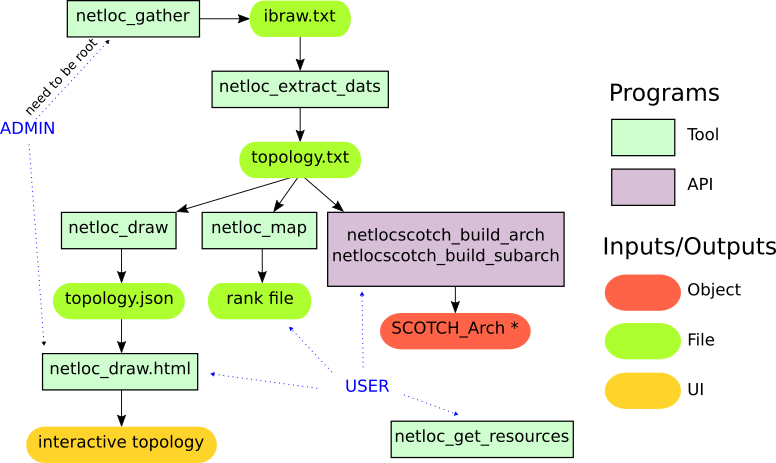
\includegraphics[width=9cm]{netloc_design.png}}
\end{DoxyImageNoCaption}


 \hypertarget{a00396_supportednetworks}{}\subsection{Supported Networks}\label{a00396_supportednetworks}
For now, only Infini\+Band (See \hyperlink{a00396_netloc_setup}{Setup}) is supported, but it is planned to be extended it very soon.

 \hypertarget{a00396_netloc_installation}{}\section{Netloc Installation}\label{a00396_netloc_installation}
The generic installation procedure for both hwloc and netloc is described in \hyperlink{index_common_installation}{Installation}.

Note that netloc is currently not supported on as many platforms as the original hwloc project. netloc is enabled by default when supported, or can be disabled by passing {\ttfamily -\/-\/disable-\/netloc} to the configure command-\/line.

 \hypertarget{a00396_netloc_setup}{}\section{Setup}\label{a00396_netloc_setup}
To use Netloc tools, we need two steps. The first step consists in getting information about network directly from tools distributed by manufacturers. For Infiniband, for instance, this operation needs privileges to access to the network device. For this step we have wrappers in Netloc that will call the right tools with the right options.

The second step will transform the raw files generated by manufacturer tools, into files in a format readable by Netloc tools, and that will not depend on network technologies.

To be clear, let\textquotesingle{}s take an example with Infiniband. This first step is handled by {\ttfamily netloc\+\_\+ib\+\_\+gather\+\_\+raw} that will call {\ttfamily ibnetdiscover} and {\ttfamily ibroutes} tools to generate the necessary raw data files. The step has to be run by an administrator, since the Infiniband tools need to access to the network device.

\begin{DoxyVerb}shell$ netloc_ib_gather_raw --help
Usage: netloc_ib_gather_raw [options] <outdir>
  Dumps topology information to <outdir>/ib-raw/
  Subnets are guessed from the <outdir>/hwloc/ directory where
  the hwloc XML exports of some nodes are stored.
Options:
 --sudo
    Pass sudo to internal ibnetdiscover and ibroute invocations.
    Useful when the entire script cannot run as root.
 --hwloc-dir <dir>
    Use <dir> instead of <outdir>/hwloc/ for hwloc XML exports.
 --force-subnet [<subnet>:]<board>:<port> to force the discovery
    Do not guess subnets from hwloc XML exports.
    Force discovery on local board <board> port <port>
    and optionally force the subnet id <subnet>
    instead of reading it from the first GID.
    Examples: --force-subnet mlx4_0:1
              --force-subnet fe80:0000:0000:0000:mlx4_0:1
 --ibnetdiscover /path/to/ibnetdiscover
 --ibroute /path/to/ibroute
    Specify exact location of programs. Default is /usr/bin/<program>
 --sleep <n>
    Sleep for <n> seconds between invocations of programs probing the network
 --ignore-errors
    Ignore errors from ibnetdiscover and ibroute, assume their outputs are ok
 --force -f
    Always rediscover to overwrite existing files without asking
 --verbose -v
    Add verbose messages
 --dry-run
    Do not actually run programs or modify anything
 --help -h
    Show this help

shell$ ./netloc_ib_gather_raw /home/netloc/data
WARNING: Not running as root.
Using /home/netloc/data/hwloc as hwloc lstopo XML directory.

Exporting local node hwloc XML...
  Running lstopo-no-graphics...

Found 1 subnets in hwloc directory:
 Subnet fe80:0000:0000:0000 is locally accessible from board qib0 port 1.

Looking at fe80:0000:0000:0000 (through local board qib0 port 1)...
 Running ibnetdiscover...
 Getting routes...
  Running ibroute for switch 'QLogic 12800-180 GUID=0x00066a00e8001310 L112' LID 18...
  Running ibroute for switch 'QLogic 12800-180 GUID=0x00066a00e8001310 L108' LID 20...
  Running ibroute for switch 'QLogic 12800-180 GUID=0x00066a00e8001310 L102' LID 23...
  Running ibroute for switch 'QLogic 12800-180 GUID=0x00066a00e8001310 L104' LID 25...
  Running ibroute for switch 'QLogic 12800-180 GUID=0x00066a00e8001310 L106' LID 24...
  Running ibroute for switch 'QLogic 12800-180 GUID=0x00066a00e8001310 L114' LID 22...
  Running ibroute for switch 'QLogic 12800-180 GUID=0x00066a00e8001310 L116' LID 21...
  Running ibroute for switch 'QLogic 12800-180 GUID=0x00066a00e8001310 L109' LID 12...
  Running ibroute for switch 'QLogic 12800-180 GUID=0x00066a00e8001310 L111' LID 11...
  Running ibroute for switch 'QLogic 12800-180 GUID=0x00066a00e8001310 L107' LID 13...
  Running ibroute for switch 'QLogic 12800-180 GUID=0x00066a00e8001310 L103' LID 17...
  Running ibroute for switch 'QLogic 12800-180 GUID=0x00066a00e8001310 L105' LID 16...
  Running ibroute for switch 'QLogic 12800-180 GUID=0x00066a00e8001310 L113' LID 15...
\end{DoxyVerb}


The second step, that can be done by a regular user, is done by the tool {\ttfamily netloc\+\_\+ib\+\_\+extract\+\_\+dats}.

\begin{DoxyVerb}shell$ netloc_ib_extract_dats --help
Usage: netloc_ib_extract_dats <path to input raw data files> <output path> [--hwloc-dir
<hwloc xml path>]
        hwloc-dir can be an absolute path or a relative path from output path

shell$ netloc_ib_extract_dats /home/netloc/data/ib-raw /home/netloc/data/netloc \
  --hwloc-dir ../hwloc
Read subnet: fe80:0000:0000:0000
2 partitions found
        'node'
        'admin'
\end{DoxyVerb}


 \hypertarget{a00396_netloc_draw}{}\section{Topology display}\label{a00396_netloc_draw}
Netloc provides a tool, {\ttfamily netloc\+\_\+draw.\+html}, that displays a topology in a web browser, by using a J\+S\+ON file.\hypertarget{a00396_netloc_draw_setup}{}\subsection{Generate the J\+S\+O\+N file}\label{a00396_netloc_draw_setup}
In order to display a topology, Netloc needs to generate a J\+S\+ON file corresponding to a topology. For this operation, the user must run {\ttfamily netloc\+\_\+draw\+\_\+to\+\_\+json}.

\begin{DoxyVerb}shell$ netloc_draw_to_json --help
Usage: netloc_draw_to_json <path to topology directory>

shell$ netloc_draw_to_json /home/netloc/data/netloc
\end{DoxyVerb}


The {\ttfamily netloc\+\_\+draw\+\_\+to\+\_\+json} command will write a J\+S\+ON file for each topology file found in the input directory. The output files, written also in the input directory, can be open by {\ttfamily netloc\+\_\+draw.\+html} in a web browser.\hypertarget{a00396_netloc_draw_tool}{}\subsection{Using netloc\+\_\+draw}\label{a00396_netloc_draw_tool}
Once the J\+S\+ON file is opened, the rendering is generated by the Javascript vis library for computing the position of the nodes. From the interface, it is possible to search for a specific node, to color the nodes, to expand merged switches, to show statistics, to export as an image... The user can interact with the nodes by moving them. For now, there are bugs and other nodes might move too.

The placement of the nodes is done statically if the topology is detected as a tree. If not, vis.\+js will use physics to find good positions, and it can be very time consuming.

 
\begin{DoxyImageNoCaption}
  \mbox{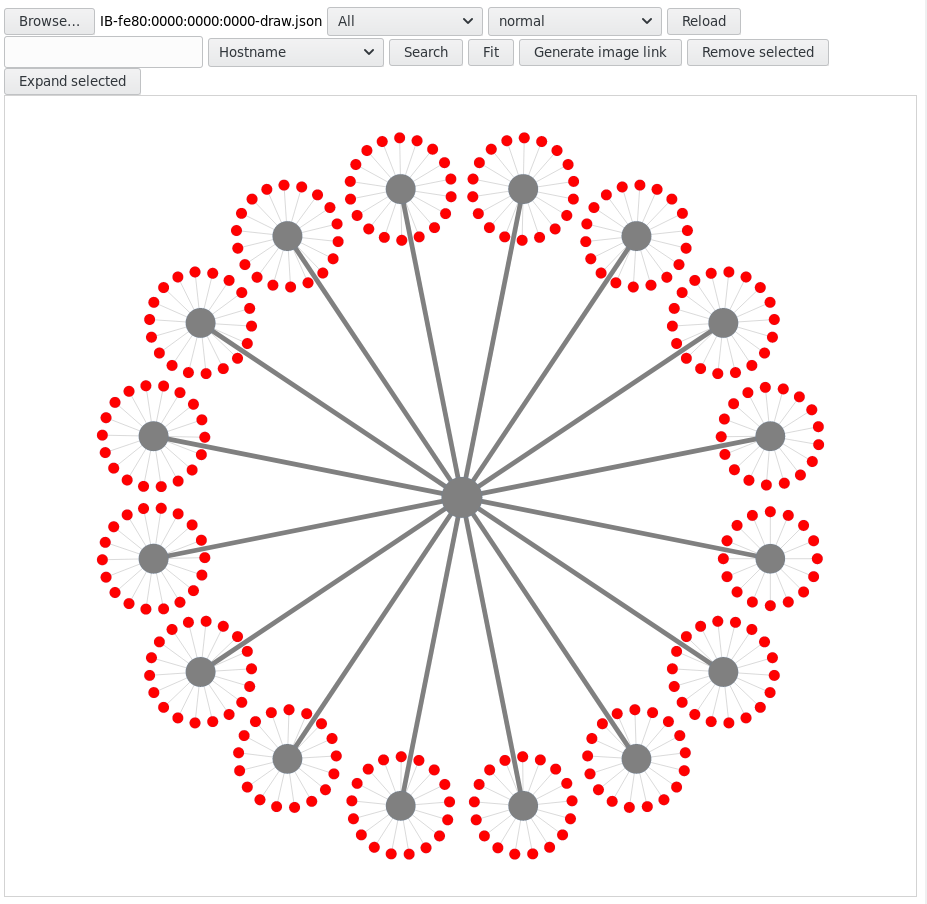
\includegraphics[width=15cm]{netloc_draw.png}}
\end{DoxyImageNoCaption}
 
\chapter{Netloc with Scotch}
\label{a00397}
\Hypertarget{a00397}


Scotch is a toolbox for graph partitioning \mbox{[}X\+XX\mbox{]}, that can do mapping between a communication graph and an architecture. Netloc interfaces with Scotch, by getting the topology of the machine and building the Scotch architecture. It is also possible to directly build a mapping file that can be given to {\ttfamily mpirun}.

 \hypertarget{a00397_scotch_intro}{}\section{Introduction}\label{a00397_scotch_intro}
Scotch is able to deal architectures to represent the topology of a complete machine. Scotch handles several types of topologies\+: complete graphs, hypercubes, fat trees, meshes, torus, and random graphs. Moreover, Scotch is able to manage parts of architectures that are called sub-\/architectures. Thus, from a complete architecture, we can create a sub-\/architecture that will represent the available resources of the complete machine.

 \hypertarget{a00397_scotch_setup}{}\section{Setup}\label{a00397_scotch_setup}
The first step in order to use Netloc tools is to discover the network. For this task, we provide tools called netloc\+\_\+gather that are wrappers to the dedicated tools provided by the manufacturer of the network, that generate the raw data given by the devices. This task needs privileges to access to the network devices. Once, this task is completed, the raw data is converted in a generic format independent to the fabric by extract\+\_\+dats. Figure 1 shows how the different modules of Netloc are linked, and what are the tools provided by Netloc.

 \hypertarget{a00397_scotch_tools_api}{}\section{Tools and A\+PI}\label{a00397_scotch_tools_api}
When the machine is discovered and all the needed files are generated as seen previously, a user can call the netlocscotch functions from the A\+PI and interact with Scotch.\hypertarget{a00397_netlocscotch_arch}{}\subsection{Build Scotch architectures}\label{a00397_netlocscotch_arch}
Netloc provides a function to export the built topology into the Scotch format. That will give the possibility to the user to play with the topology in Scotch. Since Netloc matches the discovered topology with known topologies, the Scotch architecture won’t be random graphs but known topologies also in Scotch that will lead to optimized graph algorithms. This function is called netlocscotch\+\_\+build\+\_\+arch.

When the network topology is a tree, the topology converted by netlocscotch is the complete topology of the machine containing intranode topologies from hwloc. In this case, merging the two levels results in a bigger tree. For other network topologies, the global graph created for Scotch is a generic graph since it not not (at this moment) possible to create nested known architectures.\hypertarget{a00397_netlocscotch_subarch}{}\subsection{Build Scotch sub-\/architectures}\label{a00397_netlocscotch_subarch}
Most of the time, the user does not have access to the complete machine. He uses a resource manager to run his application and he will gain access only to a set of nodes. In this case getting the Scotch architecture of the complete machine is not relevant. Fortunately, Netloc is also able to build a Scotch sub-\/architecture that will contain only the available nodes. For this operation the user needs to run a specific program, netloc\+\_\+get\+\_\+resources, that will record in a file, the lists of available nodes and available cores by using M\+PI and hwloc. From this file, the function netlocscotch\+\_\+build\+\_\+subarch will build the Scotch sub-\/architecture.\hypertarget{a00397_netlocscotch_mapping}{}\subsection{Mapping of processes}\label{a00397_netlocscotch_mapping}
A main goal in having all these data about the network topology, especially in Scotch structures, is to help the process placement. For that, we use the mapping of a process graph to the architecture provided by Scotch. As we have seen previously, Netloc is able to detect the structure of the topology and will build the adapted Scotch architecture that will be more efficient than a random structure.

In case, the network topology is not a tree, netlocscotch converts the complete topology into a generic graph. The drawback in that is the Scotch graph algorithms are less efficient. To overcome that, netlocscotch does two steps of mapping\+: first it maps the processes to the nodes, and then for each node maps the processes to the cores. We have to conduct tests to check if the method gives better results than using a generic graph directly.

The other input needed in Scotch is the process graph. Since we want to optimize the placement to decrease the communication time, a good metric for building the application graph is the amount of communications between all pairs of processes. Studies still have to be done to choose, in the most efficient way, what we take into account to define the amount of communications between the number of messages, the size of messages... This information will be transformed into a process graph.

Once we have a good mapping computed by Scotch, we can give it to the user, or Netloc can even generate the corresponding rank file useful to M\+PI. 
\chapter{Module Index}
\section{Modules}
Here is a list of all modules\+:\begin{DoxyCompactList}
\item \contentsline{section}{A\+PI version}{\pageref{a00182}}{}
\item \contentsline{section}{Object Sets (hwloc\+\_\+cpuset\+\_\+t and hwloc\+\_\+nodeset\+\_\+t)}{\pageref{a00183}}{}
\item \contentsline{section}{Object Types}{\pageref{a00184}}{}
\item \contentsline{section}{Object Structure and Attributes}{\pageref{a00185}}{}
\item \contentsline{section}{Topology Creation and Destruction}{\pageref{a00186}}{}
\item \contentsline{section}{Object levels, depths and types}{\pageref{a00187}}{}
\item \contentsline{section}{Converting between Object Types and Attributes, and Strings}{\pageref{a00188}}{}
\item \contentsline{section}{Consulting and Adding Key-\/\+Value Info Attributes}{\pageref{a00189}}{}
\item \contentsline{section}{C\+PU binding}{\pageref{a00190}}{}
\item \contentsline{section}{Memory binding}{\pageref{a00191}}{}
\item \contentsline{section}{Changing the Source of Topology Discovery}{\pageref{a00192}}{}
\item \contentsline{section}{Topology Detection Configuration and Query}{\pageref{a00193}}{}
\item \contentsline{section}{Modifying a loaded Topology}{\pageref{a00194}}{}
\item \contentsline{section}{Finding Objects inside a C\+PU set}{\pageref{a00195}}{}
\item \contentsline{section}{Finding Objects covering at least C\+PU set}{\pageref{a00196}}{}
\item \contentsline{section}{Looking at Ancestor and Child Objects}{\pageref{a00197}}{}
\item \contentsline{section}{Kinds of object Type}{\pageref{a00198}}{}
\item \contentsline{section}{Looking at Cache Objects}{\pageref{a00199}}{}
\item \contentsline{section}{Finding objects, miscellaneous helpers}{\pageref{a00200}}{}
\item \contentsline{section}{Distributing items over a topology}{\pageref{a00201}}{}
\item \contentsline{section}{C\+PU and node sets of entire topologies}{\pageref{a00202}}{}
\item \contentsline{section}{Converting between C\+PU sets and node sets}{\pageref{a00203}}{}
\item \contentsline{section}{Finding I/O objects}{\pageref{a00204}}{}
\item \contentsline{section}{The bitmap A\+PI}{\pageref{a00205}}{}
\item \contentsline{section}{Exporting Topologies to X\+ML}{\pageref{a00206}}{}
\item \contentsline{section}{Exporting Topologies to Synthetic}{\pageref{a00207}}{}
\item \contentsline{section}{Retrieve distances between objects}{\pageref{a00208}}{}
\item \contentsline{section}{Helpers for consulting distance matrices}{\pageref{a00209}}{}
\item \contentsline{section}{Add or remove distances between objects}{\pageref{a00210}}{}
\item \contentsline{section}{Comparing memory node attributes for finding where to allocate on}{\pageref{a00211}}{}
\item \contentsline{section}{Managing memory attributes}{\pageref{a00212}}{}
\item \contentsline{section}{Kinds of C\+PU cores}{\pageref{a00213}}{}
\item \contentsline{section}{Linux-\/specific helpers}{\pageref{a00214}}{}
\item \contentsline{section}{Interoperability with Linux libnuma unsigned long masks}{\pageref{a00215}}{}
\item \contentsline{section}{Interoperability with Linux libnuma bitmask}{\pageref{a00216}}{}
\item \contentsline{section}{Interoperability with glibc sched affinity}{\pageref{a00217}}{}
\item \contentsline{section}{Interoperability with Open\+CL}{\pageref{a00218}}{}
\item \contentsline{section}{Interoperability with the C\+U\+DA Driver A\+PI}{\pageref{a00219}}{}
\item \contentsline{section}{Interoperability with the C\+U\+DA Runtime A\+PI}{\pageref{a00220}}{}
\item \contentsline{section}{Interoperability with the N\+V\+I\+D\+IA Management Library}{\pageref{a00221}}{}
\item \contentsline{section}{Interoperability with the R\+O\+Cm S\+MI Management Library}{\pageref{a00222}}{}
\item \contentsline{section}{Interoperability with Open\+GL displays}{\pageref{a00223}}{}
\item \contentsline{section}{Interoperability with Open\+Fabrics}{\pageref{a00224}}{}
\item \contentsline{section}{Topology differences}{\pageref{a00225}}{}
\item \contentsline{section}{Sharing topologies between processes}{\pageref{a00226}}{}
\item \contentsline{section}{Components and Plugins\+: Discovery components}{\pageref{a00227}}{}
\item \contentsline{section}{Components and Plugins\+: Discovery backends}{\pageref{a00228}}{}
\item \contentsline{section}{Components and Plugins\+: Generic components}{\pageref{a00229}}{}
\item \contentsline{section}{Components and Plugins\+: Core functions to be used by components}{\pageref{a00230}}{}
\item \contentsline{section}{Components and Plugins\+: Filtering objects}{\pageref{a00231}}{}
\item \contentsline{section}{Components and Plugins\+: helpers for P\+CI discovery}{\pageref{a00232}}{}
\item \contentsline{section}{Components and Plugins\+: finding P\+CI objects during other discoveries}{\pageref{a00233}}{}
\item \contentsline{section}{Netloc A\+PI}{\pageref{a00234}}{}
\end{DoxyCompactList}

\chapter{Data Structure Index}
\section{Data Structures}
Here are the data structures with brief descriptions\+:\begin{DoxyCompactList}
\item\contentsline{section}{\hyperlink{a00374}{hwloc\+\_\+backend} \\*Discovery backend structure }{\pageref{a00374}}{}
\item\contentsline{section}{\hyperlink{a00266}{hwloc\+\_\+obj\+\_\+attr\+\_\+u\+::hwloc\+\_\+bridge\+\_\+attr\+\_\+s} \\*Bridge specific Object Attribues }{\pageref{a00266}}{}
\item\contentsline{section}{\hyperlink{a00254}{hwloc\+\_\+obj\+\_\+attr\+\_\+u\+::hwloc\+\_\+cache\+\_\+attr\+\_\+s} \\*Cache-\/specific Object Attributes }{\pageref{a00254}}{}
\item\contentsline{section}{\hyperlink{a00322}{hwloc\+\_\+cl\+\_\+device\+\_\+topology\+\_\+amd} }{\pageref{a00322}}{}
\item\contentsline{section}{\hyperlink{a00378}{hwloc\+\_\+component} \\*Generic component structure }{\pageref{a00378}}{}
\item\contentsline{section}{\hyperlink{a00366}{hwloc\+\_\+disc\+\_\+component} \\*Discovery component structure }{\pageref{a00366}}{}
\item\contentsline{section}{\hyperlink{a00370}{hwloc\+\_\+disc\+\_\+status} \\*Discovery status structure }{\pageref{a00370}}{}
\item\contentsline{section}{\hyperlink{a00310}{hwloc\+\_\+distances\+\_\+s} \\*Matrix of distances between a set of objects }{\pageref{a00310}}{}
\item\contentsline{section}{\hyperlink{a00258}{hwloc\+\_\+obj\+\_\+attr\+\_\+u\+::hwloc\+\_\+group\+\_\+attr\+\_\+s} \\*Group-\/specific Object Attributes }{\pageref{a00258}}{}
\item\contentsline{section}{\hyperlink{a00286}{hwloc\+\_\+info\+\_\+s} \\*Object info }{\pageref{a00286}}{}
\item\contentsline{section}{\hyperlink{a00314}{hwloc\+\_\+location} \\*Where to measure attributes from }{\pageref{a00314}}{}
\item\contentsline{section}{\hyperlink{a00318}{hwloc\+\_\+location\+::hwloc\+\_\+location\+\_\+u} \\*Actual location }{\pageref{a00318}}{}
\item\contentsline{section}{\hyperlink{a00250}{hwloc\+\_\+obj\+\_\+attr\+\_\+u\+::hwloc\+\_\+numanode\+\_\+attr\+\_\+s\+::hwloc\+\_\+memory\+\_\+page\+\_\+type\+\_\+s} \\*Array of local memory page types, {\ttfamily N\+U\+LL} if no local memory and {\ttfamily page\+\_\+types} is 0 }{\pageref{a00250}}{}
\item\contentsline{section}{\hyperlink{a00246}{hwloc\+\_\+obj\+\_\+attr\+\_\+u\+::hwloc\+\_\+numanode\+\_\+attr\+\_\+s} \\*N\+U\+MA node-\/specific Object Attributes }{\pageref{a00246}}{}
\item\contentsline{section}{\hyperlink{a00238}{hwloc\+\_\+obj} \\*Structure of a topology object }{\pageref{a00238}}{}
\item\contentsline{section}{\hyperlink{a00242}{hwloc\+\_\+obj\+\_\+attr\+\_\+u} \\*Object type-\/specific Attributes }{\pageref{a00242}}{}
\item\contentsline{section}{\hyperlink{a00282}{hwloc\+\_\+obj\+\_\+attr\+\_\+u\+::hwloc\+\_\+osdev\+\_\+attr\+\_\+s} \\*OS Device specific Object Attributes }{\pageref{a00282}}{}
\item\contentsline{section}{\hyperlink{a00262}{hwloc\+\_\+obj\+\_\+attr\+\_\+u\+::hwloc\+\_\+pcidev\+\_\+attr\+\_\+s} \\*P\+CI Device specific Object Attributes }{\pageref{a00262}}{}
\item\contentsline{section}{\hyperlink{a00294}{hwloc\+\_\+topology\+\_\+cpubind\+\_\+support} \\*Flags describing actual PU binding support for this topology }{\pageref{a00294}}{}
\item\contentsline{section}{\hyperlink{a00354}{hwloc\+\_\+topology\+\_\+diff\+\_\+u\+::hwloc\+\_\+topology\+\_\+diff\+\_\+generic\+\_\+s} }{\pageref{a00354}}{}
\item\contentsline{section}{\hyperlink{a00338}{hwloc\+\_\+topology\+\_\+diff\+\_\+obj\+\_\+attr\+\_\+u\+::hwloc\+\_\+topology\+\_\+diff\+\_\+obj\+\_\+attr\+\_\+generic\+\_\+s} }{\pageref{a00338}}{}
\item\contentsline{section}{\hyperlink{a00358}{hwloc\+\_\+topology\+\_\+diff\+\_\+u\+::hwloc\+\_\+topology\+\_\+diff\+\_\+obj\+\_\+attr\+\_\+s} }{\pageref{a00358}}{}
\item\contentsline{section}{\hyperlink{a00346}{hwloc\+\_\+topology\+\_\+diff\+\_\+obj\+\_\+attr\+\_\+u\+::hwloc\+\_\+topology\+\_\+diff\+\_\+obj\+\_\+attr\+\_\+string\+\_\+s} \\*String attribute modification with an optional name }{\pageref{a00346}}{}
\item\contentsline{section}{\hyperlink{a00334}{hwloc\+\_\+topology\+\_\+diff\+\_\+obj\+\_\+attr\+\_\+u} \\*One object attribute difference }{\pageref{a00334}}{}
\item\contentsline{section}{\hyperlink{a00342}{hwloc\+\_\+topology\+\_\+diff\+\_\+obj\+\_\+attr\+\_\+u\+::hwloc\+\_\+topology\+\_\+diff\+\_\+obj\+\_\+attr\+\_\+uint64\+\_\+s} \\*Integer attribute modification with an optional index }{\pageref{a00342}}{}
\item\contentsline{section}{\hyperlink{a00362}{hwloc\+\_\+topology\+\_\+diff\+\_\+u\+::hwloc\+\_\+topology\+\_\+diff\+\_\+too\+\_\+complex\+\_\+s} }{\pageref{a00362}}{}
\item\contentsline{section}{\hyperlink{a00350}{hwloc\+\_\+topology\+\_\+diff\+\_\+u} \\*One element of a difference list between two topologies }{\pageref{a00350}}{}
\item\contentsline{section}{\hyperlink{a00290}{hwloc\+\_\+topology\+\_\+discovery\+\_\+support} \\*Flags describing actual discovery support for this topology }{\pageref{a00290}}{}
\item\contentsline{section}{\hyperlink{a00298}{hwloc\+\_\+topology\+\_\+membind\+\_\+support} \\*Flags describing actual memory binding support for this topology }{\pageref{a00298}}{}
\item\contentsline{section}{\hyperlink{a00302}{hwloc\+\_\+topology\+\_\+misc\+\_\+support} \\*Flags describing miscellaneous features }{\pageref{a00302}}{}
\item\contentsline{section}{\hyperlink{a00306}{hwloc\+\_\+topology\+\_\+support} \\*Set of flags describing actual support for this topology }{\pageref{a00306}}{}
\end{DoxyCompactList}

\chapter{Module Documentation}
\hypertarget{a00182}{}\section{A\+PI version}
\label{a00182}\index{A\+P\+I version@{A\+P\+I version}}
\subsection*{Macros}
\begin{DoxyCompactItemize}
\item 
\#define \hyperlink{a00182_ga8f4dfb8eef138af55dd1a0fa802e5476}{H\+W\+L\+O\+C\+\_\+\+A\+P\+I\+\_\+\+V\+E\+R\+S\+I\+ON}~0x00020400
\item 
\#define \hyperlink{a00182_gaac5bc1f46f55e10ef0141a68ce70e21f}{H\+W\+L\+O\+C\+\_\+\+C\+O\+M\+P\+O\+N\+E\+N\+T\+\_\+\+A\+BI}~7
\end{DoxyCompactItemize}
\subsection*{Functions}
\begin{DoxyCompactItemize}
\item 
unsigned \hyperlink{a00182_ga9c0b50c98add1adf57ed1ce85bb5190d}{hwloc\+\_\+get\+\_\+api\+\_\+version} (void)
\end{DoxyCompactItemize}


\subsection{Detailed Description}


\subsection{Macro Definition Documentation}
\mbox{\Hypertarget{a00182_ga8f4dfb8eef138af55dd1a0fa802e5476}\label{a00182_ga8f4dfb8eef138af55dd1a0fa802e5476}} 
\index{A\+P\+I version@{A\+P\+I version}!H\+W\+L\+O\+C\+\_\+\+A\+P\+I\+\_\+\+V\+E\+R\+S\+I\+ON@{H\+W\+L\+O\+C\+\_\+\+A\+P\+I\+\_\+\+V\+E\+R\+S\+I\+ON}}
\index{H\+W\+L\+O\+C\+\_\+\+A\+P\+I\+\_\+\+V\+E\+R\+S\+I\+ON@{H\+W\+L\+O\+C\+\_\+\+A\+P\+I\+\_\+\+V\+E\+R\+S\+I\+ON}!A\+P\+I version@{A\+P\+I version}}
\subsubsection{\texorpdfstring{H\+W\+L\+O\+C\+\_\+\+A\+P\+I\+\_\+\+V\+E\+R\+S\+I\+ON}{HWLOC\_API\_VERSION}}
{\footnotesize\ttfamily \#define H\+W\+L\+O\+C\+\_\+\+A\+P\+I\+\_\+\+V\+E\+R\+S\+I\+ON~0x00020400}



Indicate at build time which hwloc A\+PI version is being used. 

This number is updated to (X$<$$<$16)+(Y$<$$<$8)+Z when a new release X.\+Y.\+Z actually modifies the A\+PI.

Users may check for available features at build time using this number (see \hyperlink{a00394_faq_version_api}{How do I handle A\+PI changes?}).

\begin{DoxyNote}{Note}
This should not be confused with H\+W\+L\+O\+C\+\_\+\+V\+E\+R\+S\+I\+ON, the library version. Two stable releases of the same series usually have the same \hyperlink{a00182_ga8f4dfb8eef138af55dd1a0fa802e5476}{H\+W\+L\+O\+C\+\_\+\+A\+P\+I\+\_\+\+V\+E\+R\+S\+I\+ON} even if their H\+W\+L\+O\+C\+\_\+\+V\+E\+R\+S\+I\+ON are different. 
\end{DoxyNote}
\mbox{\Hypertarget{a00182_gaac5bc1f46f55e10ef0141a68ce70e21f}\label{a00182_gaac5bc1f46f55e10ef0141a68ce70e21f}} 
\index{A\+P\+I version@{A\+P\+I version}!H\+W\+L\+O\+C\+\_\+\+C\+O\+M\+P\+O\+N\+E\+N\+T\+\_\+\+A\+BI@{H\+W\+L\+O\+C\+\_\+\+C\+O\+M\+P\+O\+N\+E\+N\+T\+\_\+\+A\+BI}}
\index{H\+W\+L\+O\+C\+\_\+\+C\+O\+M\+P\+O\+N\+E\+N\+T\+\_\+\+A\+BI@{H\+W\+L\+O\+C\+\_\+\+C\+O\+M\+P\+O\+N\+E\+N\+T\+\_\+\+A\+BI}!A\+P\+I version@{A\+P\+I version}}
\subsubsection{\texorpdfstring{H\+W\+L\+O\+C\+\_\+\+C\+O\+M\+P\+O\+N\+E\+N\+T\+\_\+\+A\+BI}{HWLOC\_COMPONENT\_ABI}}
{\footnotesize\ttfamily \#define H\+W\+L\+O\+C\+\_\+\+C\+O\+M\+P\+O\+N\+E\+N\+T\+\_\+\+A\+BI~7}



Current component and plugin A\+BI version (see \hyperlink{a00176_source}{hwloc/plugins.\+h}) 



\subsection{Function Documentation}
\mbox{\Hypertarget{a00182_ga9c0b50c98add1adf57ed1ce85bb5190d}\label{a00182_ga9c0b50c98add1adf57ed1ce85bb5190d}} 
\index{A\+P\+I version@{A\+P\+I version}!hwloc\+\_\+get\+\_\+api\+\_\+version@{hwloc\+\_\+get\+\_\+api\+\_\+version}}
\index{hwloc\+\_\+get\+\_\+api\+\_\+version@{hwloc\+\_\+get\+\_\+api\+\_\+version}!A\+P\+I version@{A\+P\+I version}}
\subsubsection{\texorpdfstring{hwloc\+\_\+get\+\_\+api\+\_\+version()}{hwloc\_get\_api\_version()}}
{\footnotesize\ttfamily unsigned hwloc\+\_\+get\+\_\+api\+\_\+version (\begin{DoxyParamCaption}\item[{void}]{ }\end{DoxyParamCaption})}



Indicate at runtime which hwloc A\+PI version was used at build time. 

Should be \hyperlink{a00182_ga8f4dfb8eef138af55dd1a0fa802e5476}{H\+W\+L\+O\+C\+\_\+\+A\+P\+I\+\_\+\+V\+E\+R\+S\+I\+ON} if running on the same version. 
\hypertarget{a00183}{}\section{Object Sets (hwloc\+\_\+cpuset\+\_\+t and hwloc\+\_\+nodeset\+\_\+t)}
\label{a00183}\index{Object Sets (hwloc\+\_\+cpuset\+\_\+t and hwloc\+\_\+nodeset\+\_\+t)@{Object Sets (hwloc\+\_\+cpuset\+\_\+t and hwloc\+\_\+nodeset\+\_\+t)}}
\subsection*{Typedefs}
\begin{DoxyCompactItemize}
\item 
typedef \hyperlink{a00205_gaa3c2bf4c776d603dcebbb61b0c923d84}{hwloc\+\_\+bitmap\+\_\+t} \hyperlink{a00183_ga4bbf39b68b6f568fb92739e7c0ea7801}{hwloc\+\_\+cpuset\+\_\+t}
\item 
typedef \hyperlink{a00205_gae991a108af01d408be2776c5b2c467b2}{hwloc\+\_\+const\+\_\+bitmap\+\_\+t} \hyperlink{a00183_ga1f784433e9b606261f62d1134f6a3b25}{hwloc\+\_\+const\+\_\+cpuset\+\_\+t}
\item 
typedef \hyperlink{a00205_gaa3c2bf4c776d603dcebbb61b0c923d84}{hwloc\+\_\+bitmap\+\_\+t} \hyperlink{a00183_ga37e35730fa7e775b5bb0afe893d6d508}{hwloc\+\_\+nodeset\+\_\+t}
\item 
typedef \hyperlink{a00205_gae991a108af01d408be2776c5b2c467b2}{hwloc\+\_\+const\+\_\+bitmap\+\_\+t} \hyperlink{a00183_ga2f5276235841ad66a79bedad16a5a10c}{hwloc\+\_\+const\+\_\+nodeset\+\_\+t}
\end{DoxyCompactItemize}


\subsection{Detailed Description}
Hwloc uses bitmaps to represent two distinct kinds of object sets\+: C\+PU sets (\hyperlink{a00183_ga4bbf39b68b6f568fb92739e7c0ea7801}{hwloc\+\_\+cpuset\+\_\+t}) and N\+U\+MA node sets (\hyperlink{a00183_ga37e35730fa7e775b5bb0afe893d6d508}{hwloc\+\_\+nodeset\+\_\+t}). These types are both typedefs to a common back end type (\hyperlink{a00205_gaa3c2bf4c776d603dcebbb61b0c923d84}{hwloc\+\_\+bitmap\+\_\+t}), and therefore all the hwloc bitmap functions are applicable to both \hyperlink{a00183_ga4bbf39b68b6f568fb92739e7c0ea7801}{hwloc\+\_\+cpuset\+\_\+t} and \hyperlink{a00183_ga37e35730fa7e775b5bb0afe893d6d508}{hwloc\+\_\+nodeset\+\_\+t} (see \hyperlink{a00205}{The bitmap A\+PI}).

The rationale for having two different types is that even though the actions one wants to perform on these types are the same (e.\+g., enable and disable individual items in the set/mask), they\textquotesingle{}re used in very different contexts\+: one for specifying which processors to use and one for specifying which N\+U\+MA nodes to use. Hence, the name difference is really just to reflect the intent of where the type is used. 

\subsection{Typedef Documentation}
\mbox{\Hypertarget{a00183_ga1f784433e9b606261f62d1134f6a3b25}\label{a00183_ga1f784433e9b606261f62d1134f6a3b25}} 
\index{Object Sets (hwloc\+\_\+cpuset\+\_\+t and hwloc\+\_\+nodeset\+\_\+t)@{Object Sets (hwloc\+\_\+cpuset\+\_\+t and hwloc\+\_\+nodeset\+\_\+t)}!hwloc\+\_\+const\+\_\+cpuset\+\_\+t@{hwloc\+\_\+const\+\_\+cpuset\+\_\+t}}
\index{hwloc\+\_\+const\+\_\+cpuset\+\_\+t@{hwloc\+\_\+const\+\_\+cpuset\+\_\+t}!Object Sets (hwloc\+\_\+cpuset\+\_\+t and hwloc\+\_\+nodeset\+\_\+t)@{Object Sets (hwloc\+\_\+cpuset\+\_\+t and hwloc\+\_\+nodeset\+\_\+t)}}
\subsubsection{\texorpdfstring{hwloc\+\_\+const\+\_\+cpuset\+\_\+t}{hwloc\_const\_cpuset\_t}}
{\footnotesize\ttfamily typedef \hyperlink{a00205_gae991a108af01d408be2776c5b2c467b2}{hwloc\+\_\+const\+\_\+bitmap\+\_\+t} \hyperlink{a00183_ga1f784433e9b606261f62d1134f6a3b25}{hwloc\+\_\+const\+\_\+cpuset\+\_\+t}}



A non-\/modifiable \hyperlink{a00183_ga4bbf39b68b6f568fb92739e7c0ea7801}{hwloc\+\_\+cpuset\+\_\+t}. 

\mbox{\Hypertarget{a00183_ga2f5276235841ad66a79bedad16a5a10c}\label{a00183_ga2f5276235841ad66a79bedad16a5a10c}} 
\index{Object Sets (hwloc\+\_\+cpuset\+\_\+t and hwloc\+\_\+nodeset\+\_\+t)@{Object Sets (hwloc\+\_\+cpuset\+\_\+t and hwloc\+\_\+nodeset\+\_\+t)}!hwloc\+\_\+const\+\_\+nodeset\+\_\+t@{hwloc\+\_\+const\+\_\+nodeset\+\_\+t}}
\index{hwloc\+\_\+const\+\_\+nodeset\+\_\+t@{hwloc\+\_\+const\+\_\+nodeset\+\_\+t}!Object Sets (hwloc\+\_\+cpuset\+\_\+t and hwloc\+\_\+nodeset\+\_\+t)@{Object Sets (hwloc\+\_\+cpuset\+\_\+t and hwloc\+\_\+nodeset\+\_\+t)}}
\subsubsection{\texorpdfstring{hwloc\+\_\+const\+\_\+nodeset\+\_\+t}{hwloc\_const\_nodeset\_t}}
{\footnotesize\ttfamily typedef \hyperlink{a00205_gae991a108af01d408be2776c5b2c467b2}{hwloc\+\_\+const\+\_\+bitmap\+\_\+t} \hyperlink{a00183_ga2f5276235841ad66a79bedad16a5a10c}{hwloc\+\_\+const\+\_\+nodeset\+\_\+t}}



A non-\/modifiable \hyperlink{a00183_ga37e35730fa7e775b5bb0afe893d6d508}{hwloc\+\_\+nodeset\+\_\+t}. 

\mbox{\Hypertarget{a00183_ga4bbf39b68b6f568fb92739e7c0ea7801}\label{a00183_ga4bbf39b68b6f568fb92739e7c0ea7801}} 
\index{Object Sets (hwloc\+\_\+cpuset\+\_\+t and hwloc\+\_\+nodeset\+\_\+t)@{Object Sets (hwloc\+\_\+cpuset\+\_\+t and hwloc\+\_\+nodeset\+\_\+t)}!hwloc\+\_\+cpuset\+\_\+t@{hwloc\+\_\+cpuset\+\_\+t}}
\index{hwloc\+\_\+cpuset\+\_\+t@{hwloc\+\_\+cpuset\+\_\+t}!Object Sets (hwloc\+\_\+cpuset\+\_\+t and hwloc\+\_\+nodeset\+\_\+t)@{Object Sets (hwloc\+\_\+cpuset\+\_\+t and hwloc\+\_\+nodeset\+\_\+t)}}
\subsubsection{\texorpdfstring{hwloc\+\_\+cpuset\+\_\+t}{hwloc\_cpuset\_t}}
{\footnotesize\ttfamily typedef \hyperlink{a00205_gaa3c2bf4c776d603dcebbb61b0c923d84}{hwloc\+\_\+bitmap\+\_\+t} \hyperlink{a00183_ga4bbf39b68b6f568fb92739e7c0ea7801}{hwloc\+\_\+cpuset\+\_\+t}}



A C\+PU set is a bitmap whose bits are set according to C\+PU physical OS indexes. 

It may be consulted and modified with the bitmap A\+PI as any \hyperlink{a00205_gaa3c2bf4c776d603dcebbb61b0c923d84}{hwloc\+\_\+bitmap\+\_\+t} (see \hyperlink{a00125_source}{hwloc/bitmap.\+h}).

Each bit may be converted into a PU object using \hyperlink{a00200_ga751c238a4931db5cc0ca3181b7dd7479}{hwloc\+\_\+get\+\_\+pu\+\_\+obj\+\_\+by\+\_\+os\+\_\+index()}. \mbox{\Hypertarget{a00183_ga37e35730fa7e775b5bb0afe893d6d508}\label{a00183_ga37e35730fa7e775b5bb0afe893d6d508}} 
\index{Object Sets (hwloc\+\_\+cpuset\+\_\+t and hwloc\+\_\+nodeset\+\_\+t)@{Object Sets (hwloc\+\_\+cpuset\+\_\+t and hwloc\+\_\+nodeset\+\_\+t)}!hwloc\+\_\+nodeset\+\_\+t@{hwloc\+\_\+nodeset\+\_\+t}}
\index{hwloc\+\_\+nodeset\+\_\+t@{hwloc\+\_\+nodeset\+\_\+t}!Object Sets (hwloc\+\_\+cpuset\+\_\+t and hwloc\+\_\+nodeset\+\_\+t)@{Object Sets (hwloc\+\_\+cpuset\+\_\+t and hwloc\+\_\+nodeset\+\_\+t)}}
\subsubsection{\texorpdfstring{hwloc\+\_\+nodeset\+\_\+t}{hwloc\_nodeset\_t}}
{\footnotesize\ttfamily typedef \hyperlink{a00205_gaa3c2bf4c776d603dcebbb61b0c923d84}{hwloc\+\_\+bitmap\+\_\+t} \hyperlink{a00183_ga37e35730fa7e775b5bb0afe893d6d508}{hwloc\+\_\+nodeset\+\_\+t}}



A node set is a bitmap whose bits are set according to N\+U\+MA memory node physical OS indexes. 

It may be consulted and modified with the bitmap A\+PI as any \hyperlink{a00205_gaa3c2bf4c776d603dcebbb61b0c923d84}{hwloc\+\_\+bitmap\+\_\+t} (see \hyperlink{a00125_source}{hwloc/bitmap.\+h}). Each bit may be converted into a N\+U\+MA node object using \hyperlink{a00200_gab89d9ed9edfaa3dd526fb6ee1a1618ea}{hwloc\+\_\+get\+\_\+numanode\+\_\+obj\+\_\+by\+\_\+os\+\_\+index()}.

When binding memory on a system without any N\+U\+MA node, the single main memory bank is considered as N\+U\+MA node \#0.

See also \hyperlink{a00203}{Converting between C\+PU sets and node sets}. 
\hypertarget{a00184}{}\section{Object Types}
\label{a00184}\index{Object Types@{Object Types}}
\subsection*{Macros}
\begin{DoxyCompactItemize}
\item 
\#define \hyperlink{a00184_ga3b6e4128e9fe773863b123fa6e4a080b}{H\+W\+L\+O\+C\+\_\+\+T\+Y\+P\+E\+\_\+\+U\+N\+O\+R\+D\+E\+R\+ED}
\end{DoxyCompactItemize}
\subsection*{Typedefs}
\begin{DoxyCompactItemize}
\item 
typedef enum \hyperlink{a00184_ga791c9875c8fe20f3e1e5871e0657e59b}{hwloc\+\_\+obj\+\_\+cache\+\_\+type\+\_\+e} \hyperlink{a00184_gab6e1e7efedae8b341f3ee14fbe53d66c}{hwloc\+\_\+obj\+\_\+cache\+\_\+type\+\_\+t}
\item 
typedef enum \hyperlink{a00184_ga48a4803c72574191d7ead1c62aaf9860}{hwloc\+\_\+obj\+\_\+bridge\+\_\+type\+\_\+e} \hyperlink{a00184_ga0a947e8c5adcc729b126bd09c01a0153}{hwloc\+\_\+obj\+\_\+bridge\+\_\+type\+\_\+t}
\item 
typedef enum \hyperlink{a00184_ga64f5d539df299c97ae80ce53fc4b56c0}{hwloc\+\_\+obj\+\_\+osdev\+\_\+type\+\_\+e} \hyperlink{a00184_ga90c1e82a60ba5871d07645169e636987}{hwloc\+\_\+obj\+\_\+osdev\+\_\+type\+\_\+t}
\end{DoxyCompactItemize}
\subsection*{Enumerations}
\begin{DoxyCompactItemize}
\item 
enum \hyperlink{a00184_gacd37bb612667dc437d66bfb175a8dc55}{hwloc\+\_\+obj\+\_\+type\+\_\+t} \{ \newline
\hyperlink{a00184_ggacd37bb612667dc437d66bfb175a8dc55a3f4e83ffc4a259354959ae8a9eaa2a80}{H\+W\+L\+O\+C\+\_\+\+O\+B\+J\+\_\+\+M\+A\+C\+H\+I\+NE}, 
\hyperlink{a00184_ggacd37bb612667dc437d66bfb175a8dc55ab16ab8c0dbffc234921d86f3dfb63129}{H\+W\+L\+O\+C\+\_\+\+O\+B\+J\+\_\+\+P\+A\+C\+K\+A\+GE}, 
\hyperlink{a00184_ggacd37bb612667dc437d66bfb175a8dc55ac793958f330bca371aa1535de8aff45f}{H\+W\+L\+O\+C\+\_\+\+O\+B\+J\+\_\+\+C\+O\+RE}, 
\hyperlink{a00184_ggacd37bb612667dc437d66bfb175a8dc55abca6887e80cb291353b0a0c1da83f661}{H\+W\+L\+O\+C\+\_\+\+O\+B\+J\+\_\+\+PU}, 
\newline
\hyperlink{a00184_ggacd37bb612667dc437d66bfb175a8dc55a56389b8eb2e2f74f288bb657c4e72140}{H\+W\+L\+O\+C\+\_\+\+O\+B\+J\+\_\+\+L1\+C\+A\+C\+HE}, 
\hyperlink{a00184_ggacd37bb612667dc437d66bfb175a8dc55a18f61d19fe9f4bcea978fcc68bc078fb}{H\+W\+L\+O\+C\+\_\+\+O\+B\+J\+\_\+\+L2\+C\+A\+C\+HE}, 
\hyperlink{a00184_ggacd37bb612667dc437d66bfb175a8dc55a25fae0e0514c90e3973a29866a5a837d}{H\+W\+L\+O\+C\+\_\+\+O\+B\+J\+\_\+\+L3\+C\+A\+C\+HE}, 
\hyperlink{a00184_ggacd37bb612667dc437d66bfb175a8dc55a54923bfa13df9d7e6d6dd0d5baff5f72}{H\+W\+L\+O\+C\+\_\+\+O\+B\+J\+\_\+\+L4\+C\+A\+C\+HE}, 
\newline
\hyperlink{a00184_ggacd37bb612667dc437d66bfb175a8dc55a67194c9de5e3e581c64c11d2eb1c109d}{H\+W\+L\+O\+C\+\_\+\+O\+B\+J\+\_\+\+L5\+C\+A\+C\+HE}, 
\hyperlink{a00184_ggacd37bb612667dc437d66bfb175a8dc55afa834a85d9e53836cf0db6d0bd8329b4}{H\+W\+L\+O\+C\+\_\+\+O\+B\+J\+\_\+\+L1\+I\+C\+A\+C\+HE}, 
\hyperlink{a00184_ggacd37bb612667dc437d66bfb175a8dc55a10713b7e561b8cc32544cd31b1c17f8d}{H\+W\+L\+O\+C\+\_\+\+O\+B\+J\+\_\+\+L2\+I\+C\+A\+C\+HE}, 
\hyperlink{a00184_ggacd37bb612667dc437d66bfb175a8dc55ac22850c717f07bf7ffb316fadd08d218}{H\+W\+L\+O\+C\+\_\+\+O\+B\+J\+\_\+\+L3\+I\+C\+A\+C\+HE}, 
\newline
\hyperlink{a00184_ggacd37bb612667dc437d66bfb175a8dc55a5269ef95be72f88465559d35c9b7ad56}{H\+W\+L\+O\+C\+\_\+\+O\+B\+J\+\_\+\+G\+R\+O\+UP}, 
\hyperlink{a00184_ggacd37bb612667dc437d66bfb175a8dc55a9d917a3e5497950c6d8948b8e183db5a}{H\+W\+L\+O\+C\+\_\+\+O\+B\+J\+\_\+\+N\+U\+M\+A\+N\+O\+DE}, 
\hyperlink{a00184_ggacd37bb612667dc437d66bfb175a8dc55a6825f10895fea60aca7a6ba9fe273db0}{H\+W\+L\+O\+C\+\_\+\+O\+B\+J\+\_\+\+B\+R\+I\+D\+GE}, 
\hyperlink{a00184_ggacd37bb612667dc437d66bfb175a8dc55a5d8117a54df1fbd3606ab19e42cb0ea9}{H\+W\+L\+O\+C\+\_\+\+O\+B\+J\+\_\+\+P\+C\+I\+\_\+\+D\+E\+V\+I\+CE}, 
\newline
\hyperlink{a00184_ggacd37bb612667dc437d66bfb175a8dc55a51e7280240fd9f25589cbbe538bdb075}{H\+W\+L\+O\+C\+\_\+\+O\+B\+J\+\_\+\+O\+S\+\_\+\+D\+E\+V\+I\+CE}, 
\hyperlink{a00184_ggacd37bb612667dc437d66bfb175a8dc55a19f8a6953fa91efc76bcbcdf2d22de4d}{H\+W\+L\+O\+C\+\_\+\+O\+B\+J\+\_\+\+M\+I\+SC}, 
\hyperlink{a00184_ggacd37bb612667dc437d66bfb175a8dc55a0ed5bd98974729a0c476c39e917dabd6}{H\+W\+L\+O\+C\+\_\+\+O\+B\+J\+\_\+\+M\+E\+M\+C\+A\+C\+HE}, 
\hyperlink{a00184_ggacd37bb612667dc437d66bfb175a8dc55af78bb6cde53aaaaa162a7dc420c409da}{H\+W\+L\+O\+C\+\_\+\+O\+B\+J\+\_\+\+D\+IE}
 \}
\item 
enum \hyperlink{a00184_ga791c9875c8fe20f3e1e5871e0657e59b}{hwloc\+\_\+obj\+\_\+cache\+\_\+type\+\_\+e} \{ \hyperlink{a00184_gga791c9875c8fe20f3e1e5871e0657e59ba3900b3b2db54941aac249e5a638a2d7a}{H\+W\+L\+O\+C\+\_\+\+O\+B\+J\+\_\+\+C\+A\+C\+H\+E\+\_\+\+U\+N\+I\+F\+I\+ED}, 
\hyperlink{a00184_gga791c9875c8fe20f3e1e5871e0657e59bacac60ecad4206f85aeb79bef1604b488}{H\+W\+L\+O\+C\+\_\+\+O\+B\+J\+\_\+\+C\+A\+C\+H\+E\+\_\+\+D\+A\+TA}, 
\hyperlink{a00184_gga791c9875c8fe20f3e1e5871e0657e59ba6f98b0d422b38ba90c5f5c79a11b0658}{H\+W\+L\+O\+C\+\_\+\+O\+B\+J\+\_\+\+C\+A\+C\+H\+E\+\_\+\+I\+N\+S\+T\+R\+U\+C\+T\+I\+ON}
 \}
\item 
enum \hyperlink{a00184_ga48a4803c72574191d7ead1c62aaf9860}{hwloc\+\_\+obj\+\_\+bridge\+\_\+type\+\_\+e} \{ \hyperlink{a00184_gga48a4803c72574191d7ead1c62aaf9860a2c7660f3864ad2810c1e72aad285e574}{H\+W\+L\+O\+C\+\_\+\+O\+B\+J\+\_\+\+B\+R\+I\+D\+G\+E\+\_\+\+H\+O\+ST}, 
\hyperlink{a00184_gga48a4803c72574191d7ead1c62aaf9860a8f3b4cecf3dab6073d74696d10863c60}{H\+W\+L\+O\+C\+\_\+\+O\+B\+J\+\_\+\+B\+R\+I\+D\+G\+E\+\_\+\+P\+CI}
 \}
\item 
enum \hyperlink{a00184_ga64f5d539df299c97ae80ce53fc4b56c0}{hwloc\+\_\+obj\+\_\+osdev\+\_\+type\+\_\+e} \{ \newline
\hyperlink{a00184_gga64f5d539df299c97ae80ce53fc4b56c0a689b0488c3c0d08d116751c6b9cb8871}{H\+W\+L\+O\+C\+\_\+\+O\+B\+J\+\_\+\+O\+S\+D\+E\+V\+\_\+\+B\+L\+O\+CK}, 
\hyperlink{a00184_gga64f5d539df299c97ae80ce53fc4b56c0aa3a09798ef2836abb236dc3a645ffc90}{H\+W\+L\+O\+C\+\_\+\+O\+B\+J\+\_\+\+O\+S\+D\+E\+V\+\_\+\+G\+PU}, 
\hyperlink{a00184_gga64f5d539df299c97ae80ce53fc4b56c0ab715d81155f771573c8682dffc65021b}{H\+W\+L\+O\+C\+\_\+\+O\+B\+J\+\_\+\+O\+S\+D\+E\+V\+\_\+\+N\+E\+T\+W\+O\+RK}, 
\hyperlink{a00184_gga64f5d539df299c97ae80ce53fc4b56c0a52157d03694fdae82dddd57ca8c973b6}{H\+W\+L\+O\+C\+\_\+\+O\+B\+J\+\_\+\+O\+S\+D\+E\+V\+\_\+\+O\+P\+E\+N\+F\+A\+B\+R\+I\+CS}, 
\newline
\hyperlink{a00184_gga64f5d539df299c97ae80ce53fc4b56c0a827ad1643360711a8b6c6af671366791}{H\+W\+L\+O\+C\+\_\+\+O\+B\+J\+\_\+\+O\+S\+D\+E\+V\+\_\+\+D\+MA}, 
\hyperlink{a00184_gga64f5d539df299c97ae80ce53fc4b56c0a46f8927e1c3e137eaa86cc8f6861fb83}{H\+W\+L\+O\+C\+\_\+\+O\+B\+J\+\_\+\+O\+S\+D\+E\+V\+\_\+\+C\+O\+P\+R\+OC}
 \}
\end{DoxyCompactItemize}
\subsection*{Functions}
\begin{DoxyCompactItemize}
\item 
int \hyperlink{a00184_ga1820ea0dfd8e9dca28f9ea7624df5ae2}{hwloc\+\_\+compare\+\_\+types} (\hyperlink{a00184_gacd37bb612667dc437d66bfb175a8dc55}{hwloc\+\_\+obj\+\_\+type\+\_\+t} type1, \hyperlink{a00184_gacd37bb612667dc437d66bfb175a8dc55}{hwloc\+\_\+obj\+\_\+type\+\_\+t} type2)
\end{DoxyCompactItemize}


\subsection{Detailed Description}


\subsection{Macro Definition Documentation}
\mbox{\Hypertarget{a00184_ga3b6e4128e9fe773863b123fa6e4a080b}\label{a00184_ga3b6e4128e9fe773863b123fa6e4a080b}} 
\index{Object Types@{Object Types}!H\+W\+L\+O\+C\+\_\+\+T\+Y\+P\+E\+\_\+\+U\+N\+O\+R\+D\+E\+R\+ED@{H\+W\+L\+O\+C\+\_\+\+T\+Y\+P\+E\+\_\+\+U\+N\+O\+R\+D\+E\+R\+ED}}
\index{H\+W\+L\+O\+C\+\_\+\+T\+Y\+P\+E\+\_\+\+U\+N\+O\+R\+D\+E\+R\+ED@{H\+W\+L\+O\+C\+\_\+\+T\+Y\+P\+E\+\_\+\+U\+N\+O\+R\+D\+E\+R\+ED}!Object Types@{Object Types}}
\subsubsection{\texorpdfstring{H\+W\+L\+O\+C\+\_\+\+T\+Y\+P\+E\+\_\+\+U\+N\+O\+R\+D\+E\+R\+ED}{HWLOC\_TYPE\_UNORDERED}}
{\footnotesize\ttfamily \#define H\+W\+L\+O\+C\+\_\+\+T\+Y\+P\+E\+\_\+\+U\+N\+O\+R\+D\+E\+R\+ED}



Value returned by \hyperlink{a00184_ga1820ea0dfd8e9dca28f9ea7624df5ae2}{hwloc\+\_\+compare\+\_\+types()} when types can not be compared. 



\subsection{Typedef Documentation}
\mbox{\Hypertarget{a00184_ga0a947e8c5adcc729b126bd09c01a0153}\label{a00184_ga0a947e8c5adcc729b126bd09c01a0153}} 
\index{Object Types@{Object Types}!hwloc\+\_\+obj\+\_\+bridge\+\_\+type\+\_\+t@{hwloc\+\_\+obj\+\_\+bridge\+\_\+type\+\_\+t}}
\index{hwloc\+\_\+obj\+\_\+bridge\+\_\+type\+\_\+t@{hwloc\+\_\+obj\+\_\+bridge\+\_\+type\+\_\+t}!Object Types@{Object Types}}
\subsubsection{\texorpdfstring{hwloc\+\_\+obj\+\_\+bridge\+\_\+type\+\_\+t}{hwloc\_obj\_bridge\_type\_t}}
{\footnotesize\ttfamily typedef enum \hyperlink{a00184_ga48a4803c72574191d7ead1c62aaf9860}{hwloc\+\_\+obj\+\_\+bridge\+\_\+type\+\_\+e}  \hyperlink{a00184_ga0a947e8c5adcc729b126bd09c01a0153}{hwloc\+\_\+obj\+\_\+bridge\+\_\+type\+\_\+t}}



Type of one side (upstream or downstream) of an I/O bridge. 

\mbox{\Hypertarget{a00184_gab6e1e7efedae8b341f3ee14fbe53d66c}\label{a00184_gab6e1e7efedae8b341f3ee14fbe53d66c}} 
\index{Object Types@{Object Types}!hwloc\+\_\+obj\+\_\+cache\+\_\+type\+\_\+t@{hwloc\+\_\+obj\+\_\+cache\+\_\+type\+\_\+t}}
\index{hwloc\+\_\+obj\+\_\+cache\+\_\+type\+\_\+t@{hwloc\+\_\+obj\+\_\+cache\+\_\+type\+\_\+t}!Object Types@{Object Types}}
\subsubsection{\texorpdfstring{hwloc\+\_\+obj\+\_\+cache\+\_\+type\+\_\+t}{hwloc\_obj\_cache\_type\_t}}
{\footnotesize\ttfamily typedef enum \hyperlink{a00184_ga791c9875c8fe20f3e1e5871e0657e59b}{hwloc\+\_\+obj\+\_\+cache\+\_\+type\+\_\+e}  \hyperlink{a00184_gab6e1e7efedae8b341f3ee14fbe53d66c}{hwloc\+\_\+obj\+\_\+cache\+\_\+type\+\_\+t}}



Cache type. 

\mbox{\Hypertarget{a00184_ga90c1e82a60ba5871d07645169e636987}\label{a00184_ga90c1e82a60ba5871d07645169e636987}} 
\index{Object Types@{Object Types}!hwloc\+\_\+obj\+\_\+osdev\+\_\+type\+\_\+t@{hwloc\+\_\+obj\+\_\+osdev\+\_\+type\+\_\+t}}
\index{hwloc\+\_\+obj\+\_\+osdev\+\_\+type\+\_\+t@{hwloc\+\_\+obj\+\_\+osdev\+\_\+type\+\_\+t}!Object Types@{Object Types}}
\subsubsection{\texorpdfstring{hwloc\+\_\+obj\+\_\+osdev\+\_\+type\+\_\+t}{hwloc\_obj\_osdev\_type\_t}}
{\footnotesize\ttfamily typedef enum \hyperlink{a00184_ga64f5d539df299c97ae80ce53fc4b56c0}{hwloc\+\_\+obj\+\_\+osdev\+\_\+type\+\_\+e}  \hyperlink{a00184_ga90c1e82a60ba5871d07645169e636987}{hwloc\+\_\+obj\+\_\+osdev\+\_\+type\+\_\+t}}



Type of a OS device. 



\subsection{Enumeration Type Documentation}
\mbox{\Hypertarget{a00184_ga48a4803c72574191d7ead1c62aaf9860}\label{a00184_ga48a4803c72574191d7ead1c62aaf9860}} 
\index{Object Types@{Object Types}!hwloc\+\_\+obj\+\_\+bridge\+\_\+type\+\_\+e@{hwloc\+\_\+obj\+\_\+bridge\+\_\+type\+\_\+e}}
\index{hwloc\+\_\+obj\+\_\+bridge\+\_\+type\+\_\+e@{hwloc\+\_\+obj\+\_\+bridge\+\_\+type\+\_\+e}!Object Types@{Object Types}}
\subsubsection{\texorpdfstring{hwloc\+\_\+obj\+\_\+bridge\+\_\+type\+\_\+e}{hwloc\_obj\_bridge\_type\_e}}
{\footnotesize\ttfamily enum \hyperlink{a00184_ga48a4803c72574191d7ead1c62aaf9860}{hwloc\+\_\+obj\+\_\+bridge\+\_\+type\+\_\+e}}



Type of one side (upstream or downstream) of an I/O bridge. 

\begin{DoxyEnumFields}{Enumerator}
\raisebox{\heightof{T}}[0pt][0pt]{\index{H\+W\+L\+O\+C\+\_\+\+O\+B\+J\+\_\+\+B\+R\+I\+D\+G\+E\+\_\+\+H\+O\+ST@{H\+W\+L\+O\+C\+\_\+\+O\+B\+J\+\_\+\+B\+R\+I\+D\+G\+E\+\_\+\+H\+O\+ST}!Object Types@{Object Types}}\index{Object Types@{Object Types}!H\+W\+L\+O\+C\+\_\+\+O\+B\+J\+\_\+\+B\+R\+I\+D\+G\+E\+\_\+\+H\+O\+ST@{H\+W\+L\+O\+C\+\_\+\+O\+B\+J\+\_\+\+B\+R\+I\+D\+G\+E\+\_\+\+H\+O\+ST}}}\mbox{\Hypertarget{a00184_gga48a4803c72574191d7ead1c62aaf9860a2c7660f3864ad2810c1e72aad285e574}\label{a00184_gga48a4803c72574191d7ead1c62aaf9860a2c7660f3864ad2810c1e72aad285e574}} 
H\+W\+L\+O\+C\+\_\+\+O\+B\+J\+\_\+\+B\+R\+I\+D\+G\+E\+\_\+\+H\+O\+ST&Host-\/side of a bridge, only possible upstream. \\
\hline

\raisebox{\heightof{T}}[0pt][0pt]{\index{H\+W\+L\+O\+C\+\_\+\+O\+B\+J\+\_\+\+B\+R\+I\+D\+G\+E\+\_\+\+P\+CI@{H\+W\+L\+O\+C\+\_\+\+O\+B\+J\+\_\+\+B\+R\+I\+D\+G\+E\+\_\+\+P\+CI}!Object Types@{Object Types}}\index{Object Types@{Object Types}!H\+W\+L\+O\+C\+\_\+\+O\+B\+J\+\_\+\+B\+R\+I\+D\+G\+E\+\_\+\+P\+CI@{H\+W\+L\+O\+C\+\_\+\+O\+B\+J\+\_\+\+B\+R\+I\+D\+G\+E\+\_\+\+P\+CI}}}\mbox{\Hypertarget{a00184_gga48a4803c72574191d7ead1c62aaf9860a8f3b4cecf3dab6073d74696d10863c60}\label{a00184_gga48a4803c72574191d7ead1c62aaf9860a8f3b4cecf3dab6073d74696d10863c60}} 
H\+W\+L\+O\+C\+\_\+\+O\+B\+J\+\_\+\+B\+R\+I\+D\+G\+E\+\_\+\+P\+CI&P\+C\+I-\/side of a bridge. \\
\hline

\end{DoxyEnumFields}
\mbox{\Hypertarget{a00184_ga791c9875c8fe20f3e1e5871e0657e59b}\label{a00184_ga791c9875c8fe20f3e1e5871e0657e59b}} 
\index{Object Types@{Object Types}!hwloc\+\_\+obj\+\_\+cache\+\_\+type\+\_\+e@{hwloc\+\_\+obj\+\_\+cache\+\_\+type\+\_\+e}}
\index{hwloc\+\_\+obj\+\_\+cache\+\_\+type\+\_\+e@{hwloc\+\_\+obj\+\_\+cache\+\_\+type\+\_\+e}!Object Types@{Object Types}}
\subsubsection{\texorpdfstring{hwloc\+\_\+obj\+\_\+cache\+\_\+type\+\_\+e}{hwloc\_obj\_cache\_type\_e}}
{\footnotesize\ttfamily enum \hyperlink{a00184_ga791c9875c8fe20f3e1e5871e0657e59b}{hwloc\+\_\+obj\+\_\+cache\+\_\+type\+\_\+e}}



Cache type. 

\begin{DoxyEnumFields}{Enumerator}
\raisebox{\heightof{T}}[0pt][0pt]{\index{H\+W\+L\+O\+C\+\_\+\+O\+B\+J\+\_\+\+C\+A\+C\+H\+E\+\_\+\+U\+N\+I\+F\+I\+ED@{H\+W\+L\+O\+C\+\_\+\+O\+B\+J\+\_\+\+C\+A\+C\+H\+E\+\_\+\+U\+N\+I\+F\+I\+ED}!Object Types@{Object Types}}\index{Object Types@{Object Types}!H\+W\+L\+O\+C\+\_\+\+O\+B\+J\+\_\+\+C\+A\+C\+H\+E\+\_\+\+U\+N\+I\+F\+I\+ED@{H\+W\+L\+O\+C\+\_\+\+O\+B\+J\+\_\+\+C\+A\+C\+H\+E\+\_\+\+U\+N\+I\+F\+I\+ED}}}\mbox{\Hypertarget{a00184_gga791c9875c8fe20f3e1e5871e0657e59ba3900b3b2db54941aac249e5a638a2d7a}\label{a00184_gga791c9875c8fe20f3e1e5871e0657e59ba3900b3b2db54941aac249e5a638a2d7a}} 
H\+W\+L\+O\+C\+\_\+\+O\+B\+J\+\_\+\+C\+A\+C\+H\+E\+\_\+\+U\+N\+I\+F\+I\+ED&Unified cache. \\
\hline

\raisebox{\heightof{T}}[0pt][0pt]{\index{H\+W\+L\+O\+C\+\_\+\+O\+B\+J\+\_\+\+C\+A\+C\+H\+E\+\_\+\+D\+A\+TA@{H\+W\+L\+O\+C\+\_\+\+O\+B\+J\+\_\+\+C\+A\+C\+H\+E\+\_\+\+D\+A\+TA}!Object Types@{Object Types}}\index{Object Types@{Object Types}!H\+W\+L\+O\+C\+\_\+\+O\+B\+J\+\_\+\+C\+A\+C\+H\+E\+\_\+\+D\+A\+TA@{H\+W\+L\+O\+C\+\_\+\+O\+B\+J\+\_\+\+C\+A\+C\+H\+E\+\_\+\+D\+A\+TA}}}\mbox{\Hypertarget{a00184_gga791c9875c8fe20f3e1e5871e0657e59bacac60ecad4206f85aeb79bef1604b488}\label{a00184_gga791c9875c8fe20f3e1e5871e0657e59bacac60ecad4206f85aeb79bef1604b488}} 
H\+W\+L\+O\+C\+\_\+\+O\+B\+J\+\_\+\+C\+A\+C\+H\+E\+\_\+\+D\+A\+TA&Data cache. \\
\hline

\raisebox{\heightof{T}}[0pt][0pt]{\index{H\+W\+L\+O\+C\+\_\+\+O\+B\+J\+\_\+\+C\+A\+C\+H\+E\+\_\+\+I\+N\+S\+T\+R\+U\+C\+T\+I\+ON@{H\+W\+L\+O\+C\+\_\+\+O\+B\+J\+\_\+\+C\+A\+C\+H\+E\+\_\+\+I\+N\+S\+T\+R\+U\+C\+T\+I\+ON}!Object Types@{Object Types}}\index{Object Types@{Object Types}!H\+W\+L\+O\+C\+\_\+\+O\+B\+J\+\_\+\+C\+A\+C\+H\+E\+\_\+\+I\+N\+S\+T\+R\+U\+C\+T\+I\+ON@{H\+W\+L\+O\+C\+\_\+\+O\+B\+J\+\_\+\+C\+A\+C\+H\+E\+\_\+\+I\+N\+S\+T\+R\+U\+C\+T\+I\+ON}}}\mbox{\Hypertarget{a00184_gga791c9875c8fe20f3e1e5871e0657e59ba6f98b0d422b38ba90c5f5c79a11b0658}\label{a00184_gga791c9875c8fe20f3e1e5871e0657e59ba6f98b0d422b38ba90c5f5c79a11b0658}} 
H\+W\+L\+O\+C\+\_\+\+O\+B\+J\+\_\+\+C\+A\+C\+H\+E\+\_\+\+I\+N\+S\+T\+R\+U\+C\+T\+I\+ON&Instruction cache (filtered out by default). \\
\hline

\end{DoxyEnumFields}
\mbox{\Hypertarget{a00184_ga64f5d539df299c97ae80ce53fc4b56c0}\label{a00184_ga64f5d539df299c97ae80ce53fc4b56c0}} 
\index{Object Types@{Object Types}!hwloc\+\_\+obj\+\_\+osdev\+\_\+type\+\_\+e@{hwloc\+\_\+obj\+\_\+osdev\+\_\+type\+\_\+e}}
\index{hwloc\+\_\+obj\+\_\+osdev\+\_\+type\+\_\+e@{hwloc\+\_\+obj\+\_\+osdev\+\_\+type\+\_\+e}!Object Types@{Object Types}}
\subsubsection{\texorpdfstring{hwloc\+\_\+obj\+\_\+osdev\+\_\+type\+\_\+e}{hwloc\_obj\_osdev\_type\_e}}
{\footnotesize\ttfamily enum \hyperlink{a00184_ga64f5d539df299c97ae80ce53fc4b56c0}{hwloc\+\_\+obj\+\_\+osdev\+\_\+type\+\_\+e}}



Type of a OS device. 

\begin{DoxyEnumFields}{Enumerator}
\raisebox{\heightof{T}}[0pt][0pt]{\index{H\+W\+L\+O\+C\+\_\+\+O\+B\+J\+\_\+\+O\+S\+D\+E\+V\+\_\+\+B\+L\+O\+CK@{H\+W\+L\+O\+C\+\_\+\+O\+B\+J\+\_\+\+O\+S\+D\+E\+V\+\_\+\+B\+L\+O\+CK}!Object Types@{Object Types}}\index{Object Types@{Object Types}!H\+W\+L\+O\+C\+\_\+\+O\+B\+J\+\_\+\+O\+S\+D\+E\+V\+\_\+\+B\+L\+O\+CK@{H\+W\+L\+O\+C\+\_\+\+O\+B\+J\+\_\+\+O\+S\+D\+E\+V\+\_\+\+B\+L\+O\+CK}}}\mbox{\Hypertarget{a00184_gga64f5d539df299c97ae80ce53fc4b56c0a689b0488c3c0d08d116751c6b9cb8871}\label{a00184_gga64f5d539df299c97ae80ce53fc4b56c0a689b0488c3c0d08d116751c6b9cb8871}} 
H\+W\+L\+O\+C\+\_\+\+O\+B\+J\+\_\+\+O\+S\+D\+E\+V\+\_\+\+B\+L\+O\+CK&Operating system block device, or non-\/volatile memory device. For instance \char`\"{}sda\char`\"{} or \char`\"{}dax2.\+0\char`\"{} on Linux. \\
\hline

\raisebox{\heightof{T}}[0pt][0pt]{\index{H\+W\+L\+O\+C\+\_\+\+O\+B\+J\+\_\+\+O\+S\+D\+E\+V\+\_\+\+G\+PU@{H\+W\+L\+O\+C\+\_\+\+O\+B\+J\+\_\+\+O\+S\+D\+E\+V\+\_\+\+G\+PU}!Object Types@{Object Types}}\index{Object Types@{Object Types}!H\+W\+L\+O\+C\+\_\+\+O\+B\+J\+\_\+\+O\+S\+D\+E\+V\+\_\+\+G\+PU@{H\+W\+L\+O\+C\+\_\+\+O\+B\+J\+\_\+\+O\+S\+D\+E\+V\+\_\+\+G\+PU}}}\mbox{\Hypertarget{a00184_gga64f5d539df299c97ae80ce53fc4b56c0aa3a09798ef2836abb236dc3a645ffc90}\label{a00184_gga64f5d539df299c97ae80ce53fc4b56c0aa3a09798ef2836abb236dc3a645ffc90}} 
H\+W\+L\+O\+C\+\_\+\+O\+B\+J\+\_\+\+O\+S\+D\+E\+V\+\_\+\+G\+PU&Operating system G\+PU device. For instance \char`\"{}\+:0.\+0\char`\"{} for a GL display, \char`\"{}card0\char`\"{} for a Linux D\+RM device. \\
\hline

\raisebox{\heightof{T}}[0pt][0pt]{\index{H\+W\+L\+O\+C\+\_\+\+O\+B\+J\+\_\+\+O\+S\+D\+E\+V\+\_\+\+N\+E\+T\+W\+O\+RK@{H\+W\+L\+O\+C\+\_\+\+O\+B\+J\+\_\+\+O\+S\+D\+E\+V\+\_\+\+N\+E\+T\+W\+O\+RK}!Object Types@{Object Types}}\index{Object Types@{Object Types}!H\+W\+L\+O\+C\+\_\+\+O\+B\+J\+\_\+\+O\+S\+D\+E\+V\+\_\+\+N\+E\+T\+W\+O\+RK@{H\+W\+L\+O\+C\+\_\+\+O\+B\+J\+\_\+\+O\+S\+D\+E\+V\+\_\+\+N\+E\+T\+W\+O\+RK}}}\mbox{\Hypertarget{a00184_gga64f5d539df299c97ae80ce53fc4b56c0ab715d81155f771573c8682dffc65021b}\label{a00184_gga64f5d539df299c97ae80ce53fc4b56c0ab715d81155f771573c8682dffc65021b}} 
H\+W\+L\+O\+C\+\_\+\+O\+B\+J\+\_\+\+O\+S\+D\+E\+V\+\_\+\+N\+E\+T\+W\+O\+RK&Operating system network device. For instance the \char`\"{}eth0\char`\"{} interface on Linux. \\
\hline

\raisebox{\heightof{T}}[0pt][0pt]{\index{H\+W\+L\+O\+C\+\_\+\+O\+B\+J\+\_\+\+O\+S\+D\+E\+V\+\_\+\+O\+P\+E\+N\+F\+A\+B\+R\+I\+CS@{H\+W\+L\+O\+C\+\_\+\+O\+B\+J\+\_\+\+O\+S\+D\+E\+V\+\_\+\+O\+P\+E\+N\+F\+A\+B\+R\+I\+CS}!Object Types@{Object Types}}\index{Object Types@{Object Types}!H\+W\+L\+O\+C\+\_\+\+O\+B\+J\+\_\+\+O\+S\+D\+E\+V\+\_\+\+O\+P\+E\+N\+F\+A\+B\+R\+I\+CS@{H\+W\+L\+O\+C\+\_\+\+O\+B\+J\+\_\+\+O\+S\+D\+E\+V\+\_\+\+O\+P\+E\+N\+F\+A\+B\+R\+I\+CS}}}\mbox{\Hypertarget{a00184_gga64f5d539df299c97ae80ce53fc4b56c0a52157d03694fdae82dddd57ca8c973b6}\label{a00184_gga64f5d539df299c97ae80ce53fc4b56c0a52157d03694fdae82dddd57ca8c973b6}} 
H\+W\+L\+O\+C\+\_\+\+O\+B\+J\+\_\+\+O\+S\+D\+E\+V\+\_\+\+O\+P\+E\+N\+F\+A\+B\+R\+I\+CS&Operating system openfabrics device. For instance the \char`\"{}mlx4\+\_\+0\char`\"{} Infini\+Band H\+CA, or \char`\"{}hfi1\+\_\+0\char`\"{} Omni-\/\+Path interface on Linux. \\
\hline

\raisebox{\heightof{T}}[0pt][0pt]{\index{H\+W\+L\+O\+C\+\_\+\+O\+B\+J\+\_\+\+O\+S\+D\+E\+V\+\_\+\+D\+MA@{H\+W\+L\+O\+C\+\_\+\+O\+B\+J\+\_\+\+O\+S\+D\+E\+V\+\_\+\+D\+MA}!Object Types@{Object Types}}\index{Object Types@{Object Types}!H\+W\+L\+O\+C\+\_\+\+O\+B\+J\+\_\+\+O\+S\+D\+E\+V\+\_\+\+D\+MA@{H\+W\+L\+O\+C\+\_\+\+O\+B\+J\+\_\+\+O\+S\+D\+E\+V\+\_\+\+D\+MA}}}\mbox{\Hypertarget{a00184_gga64f5d539df299c97ae80ce53fc4b56c0a827ad1643360711a8b6c6af671366791}\label{a00184_gga64f5d539df299c97ae80ce53fc4b56c0a827ad1643360711a8b6c6af671366791}} 
H\+W\+L\+O\+C\+\_\+\+O\+B\+J\+\_\+\+O\+S\+D\+E\+V\+\_\+\+D\+MA&Operating system dma engine device. For instance the \char`\"{}dma0chan0\char`\"{} D\+MA channel on Linux. \\
\hline

\raisebox{\heightof{T}}[0pt][0pt]{\index{H\+W\+L\+O\+C\+\_\+\+O\+B\+J\+\_\+\+O\+S\+D\+E\+V\+\_\+\+C\+O\+P\+R\+OC@{H\+W\+L\+O\+C\+\_\+\+O\+B\+J\+\_\+\+O\+S\+D\+E\+V\+\_\+\+C\+O\+P\+R\+OC}!Object Types@{Object Types}}\index{Object Types@{Object Types}!H\+W\+L\+O\+C\+\_\+\+O\+B\+J\+\_\+\+O\+S\+D\+E\+V\+\_\+\+C\+O\+P\+R\+OC@{H\+W\+L\+O\+C\+\_\+\+O\+B\+J\+\_\+\+O\+S\+D\+E\+V\+\_\+\+C\+O\+P\+R\+OC}}}\mbox{\Hypertarget{a00184_gga64f5d539df299c97ae80ce53fc4b56c0a46f8927e1c3e137eaa86cc8f6861fb83}\label{a00184_gga64f5d539df299c97ae80ce53fc4b56c0a46f8927e1c3e137eaa86cc8f6861fb83}} 
H\+W\+L\+O\+C\+\_\+\+O\+B\+J\+\_\+\+O\+S\+D\+E\+V\+\_\+\+C\+O\+P\+R\+OC&Operating system co-\/processor device. For instance \char`\"{}opencl0d0\char`\"{} for a Open\+CL device, \char`\"{}cuda0\char`\"{} for a C\+U\+DA device. \\
\hline

\end{DoxyEnumFields}
\mbox{\Hypertarget{a00184_gacd37bb612667dc437d66bfb175a8dc55}\label{a00184_gacd37bb612667dc437d66bfb175a8dc55}} 
\index{Object Types@{Object Types}!hwloc\+\_\+obj\+\_\+type\+\_\+t@{hwloc\+\_\+obj\+\_\+type\+\_\+t}}
\index{hwloc\+\_\+obj\+\_\+type\+\_\+t@{hwloc\+\_\+obj\+\_\+type\+\_\+t}!Object Types@{Object Types}}
\subsubsection{\texorpdfstring{hwloc\+\_\+obj\+\_\+type\+\_\+t}{hwloc\_obj\_type\_t}}
{\footnotesize\ttfamily enum \hyperlink{a00184_gacd37bb612667dc437d66bfb175a8dc55}{hwloc\+\_\+obj\+\_\+type\+\_\+t}}



Type of topology object. 

\begin{DoxyNote}{Note}
Do not rely on the ordering or completeness of the values as new ones may be defined in the future! If you need to compare types, use \hyperlink{a00184_ga1820ea0dfd8e9dca28f9ea7624df5ae2}{hwloc\+\_\+compare\+\_\+types()} instead. 
\end{DoxyNote}
\begin{DoxyEnumFields}{Enumerator}
\raisebox{\heightof{T}}[0pt][0pt]{\index{H\+W\+L\+O\+C\+\_\+\+O\+B\+J\+\_\+\+M\+A\+C\+H\+I\+NE@{H\+W\+L\+O\+C\+\_\+\+O\+B\+J\+\_\+\+M\+A\+C\+H\+I\+NE}!Object Types@{Object Types}}\index{Object Types@{Object Types}!H\+W\+L\+O\+C\+\_\+\+O\+B\+J\+\_\+\+M\+A\+C\+H\+I\+NE@{H\+W\+L\+O\+C\+\_\+\+O\+B\+J\+\_\+\+M\+A\+C\+H\+I\+NE}}}\mbox{\Hypertarget{a00184_ggacd37bb612667dc437d66bfb175a8dc55a3f4e83ffc4a259354959ae8a9eaa2a80}\label{a00184_ggacd37bb612667dc437d66bfb175a8dc55a3f4e83ffc4a259354959ae8a9eaa2a80}} 
H\+W\+L\+O\+C\+\_\+\+O\+B\+J\+\_\+\+M\+A\+C\+H\+I\+NE&Machine. A set of processors and memory with cache coherency. This type is always used for the root object of a topology, and never used anywhere else. Hence its parent is always {\ttfamily N\+U\+LL}. \\
\hline

\raisebox{\heightof{T}}[0pt][0pt]{\index{H\+W\+L\+O\+C\+\_\+\+O\+B\+J\+\_\+\+P\+A\+C\+K\+A\+GE@{H\+W\+L\+O\+C\+\_\+\+O\+B\+J\+\_\+\+P\+A\+C\+K\+A\+GE}!Object Types@{Object Types}}\index{Object Types@{Object Types}!H\+W\+L\+O\+C\+\_\+\+O\+B\+J\+\_\+\+P\+A\+C\+K\+A\+GE@{H\+W\+L\+O\+C\+\_\+\+O\+B\+J\+\_\+\+P\+A\+C\+K\+A\+GE}}}\mbox{\Hypertarget{a00184_ggacd37bb612667dc437d66bfb175a8dc55ab16ab8c0dbffc234921d86f3dfb63129}\label{a00184_ggacd37bb612667dc437d66bfb175a8dc55ab16ab8c0dbffc234921d86f3dfb63129}} 
H\+W\+L\+O\+C\+\_\+\+O\+B\+J\+\_\+\+P\+A\+C\+K\+A\+GE&Physical package. The physical package that usually gets inserted into a socket on the motherboard. A processor package usually contains multiple cores, and possibly some dies. \\
\hline

\raisebox{\heightof{T}}[0pt][0pt]{\index{H\+W\+L\+O\+C\+\_\+\+O\+B\+J\+\_\+\+C\+O\+RE@{H\+W\+L\+O\+C\+\_\+\+O\+B\+J\+\_\+\+C\+O\+RE}!Object Types@{Object Types}}\index{Object Types@{Object Types}!H\+W\+L\+O\+C\+\_\+\+O\+B\+J\+\_\+\+C\+O\+RE@{H\+W\+L\+O\+C\+\_\+\+O\+B\+J\+\_\+\+C\+O\+RE}}}\mbox{\Hypertarget{a00184_ggacd37bb612667dc437d66bfb175a8dc55ac793958f330bca371aa1535de8aff45f}\label{a00184_ggacd37bb612667dc437d66bfb175a8dc55ac793958f330bca371aa1535de8aff45f}} 
H\+W\+L\+O\+C\+\_\+\+O\+B\+J\+\_\+\+C\+O\+RE&Core. A computation unit (may be shared by several P\+Us, aka logical processors). \\
\hline

\raisebox{\heightof{T}}[0pt][0pt]{\index{H\+W\+L\+O\+C\+\_\+\+O\+B\+J\+\_\+\+PU@{H\+W\+L\+O\+C\+\_\+\+O\+B\+J\+\_\+\+PU}!Object Types@{Object Types}}\index{Object Types@{Object Types}!H\+W\+L\+O\+C\+\_\+\+O\+B\+J\+\_\+\+PU@{H\+W\+L\+O\+C\+\_\+\+O\+B\+J\+\_\+\+PU}}}\mbox{\Hypertarget{a00184_ggacd37bb612667dc437d66bfb175a8dc55abca6887e80cb291353b0a0c1da83f661}\label{a00184_ggacd37bb612667dc437d66bfb175a8dc55abca6887e80cb291353b0a0c1da83f661}} 
H\+W\+L\+O\+C\+\_\+\+O\+B\+J\+\_\+\+PU&Processing Unit, or (Logical) Processor. An execution unit (may share a core with some other logical processors, e.\+g. in the case of an S\+MT core). This is the smallest object representing C\+PU resources, it cannot have any child except Misc objects.

Objects of this kind are always reported and can thus be used as fallback when others are not. \\
\hline

\raisebox{\heightof{T}}[0pt][0pt]{\index{H\+W\+L\+O\+C\+\_\+\+O\+B\+J\+\_\+\+L1\+C\+A\+C\+HE@{H\+W\+L\+O\+C\+\_\+\+O\+B\+J\+\_\+\+L1\+C\+A\+C\+HE}!Object Types@{Object Types}}\index{Object Types@{Object Types}!H\+W\+L\+O\+C\+\_\+\+O\+B\+J\+\_\+\+L1\+C\+A\+C\+HE@{H\+W\+L\+O\+C\+\_\+\+O\+B\+J\+\_\+\+L1\+C\+A\+C\+HE}}}\mbox{\Hypertarget{a00184_ggacd37bb612667dc437d66bfb175a8dc55a56389b8eb2e2f74f288bb657c4e72140}\label{a00184_ggacd37bb612667dc437d66bfb175a8dc55a56389b8eb2e2f74f288bb657c4e72140}} 
H\+W\+L\+O\+C\+\_\+\+O\+B\+J\+\_\+\+L1\+C\+A\+C\+HE&Level 1 Data (or Unified) Cache. \\
\hline

\raisebox{\heightof{T}}[0pt][0pt]{\index{H\+W\+L\+O\+C\+\_\+\+O\+B\+J\+\_\+\+L2\+C\+A\+C\+HE@{H\+W\+L\+O\+C\+\_\+\+O\+B\+J\+\_\+\+L2\+C\+A\+C\+HE}!Object Types@{Object Types}}\index{Object Types@{Object Types}!H\+W\+L\+O\+C\+\_\+\+O\+B\+J\+\_\+\+L2\+C\+A\+C\+HE@{H\+W\+L\+O\+C\+\_\+\+O\+B\+J\+\_\+\+L2\+C\+A\+C\+HE}}}\mbox{\Hypertarget{a00184_ggacd37bb612667dc437d66bfb175a8dc55a18f61d19fe9f4bcea978fcc68bc078fb}\label{a00184_ggacd37bb612667dc437d66bfb175a8dc55a18f61d19fe9f4bcea978fcc68bc078fb}} 
H\+W\+L\+O\+C\+\_\+\+O\+B\+J\+\_\+\+L2\+C\+A\+C\+HE&Level 2 Data (or Unified) Cache. \\
\hline

\raisebox{\heightof{T}}[0pt][0pt]{\index{H\+W\+L\+O\+C\+\_\+\+O\+B\+J\+\_\+\+L3\+C\+A\+C\+HE@{H\+W\+L\+O\+C\+\_\+\+O\+B\+J\+\_\+\+L3\+C\+A\+C\+HE}!Object Types@{Object Types}}\index{Object Types@{Object Types}!H\+W\+L\+O\+C\+\_\+\+O\+B\+J\+\_\+\+L3\+C\+A\+C\+HE@{H\+W\+L\+O\+C\+\_\+\+O\+B\+J\+\_\+\+L3\+C\+A\+C\+HE}}}\mbox{\Hypertarget{a00184_ggacd37bb612667dc437d66bfb175a8dc55a25fae0e0514c90e3973a29866a5a837d}\label{a00184_ggacd37bb612667dc437d66bfb175a8dc55a25fae0e0514c90e3973a29866a5a837d}} 
H\+W\+L\+O\+C\+\_\+\+O\+B\+J\+\_\+\+L3\+C\+A\+C\+HE&Level 3 Data (or Unified) Cache. \\
\hline

\raisebox{\heightof{T}}[0pt][0pt]{\index{H\+W\+L\+O\+C\+\_\+\+O\+B\+J\+\_\+\+L4\+C\+A\+C\+HE@{H\+W\+L\+O\+C\+\_\+\+O\+B\+J\+\_\+\+L4\+C\+A\+C\+HE}!Object Types@{Object Types}}\index{Object Types@{Object Types}!H\+W\+L\+O\+C\+\_\+\+O\+B\+J\+\_\+\+L4\+C\+A\+C\+HE@{H\+W\+L\+O\+C\+\_\+\+O\+B\+J\+\_\+\+L4\+C\+A\+C\+HE}}}\mbox{\Hypertarget{a00184_ggacd37bb612667dc437d66bfb175a8dc55a54923bfa13df9d7e6d6dd0d5baff5f72}\label{a00184_ggacd37bb612667dc437d66bfb175a8dc55a54923bfa13df9d7e6d6dd0d5baff5f72}} 
H\+W\+L\+O\+C\+\_\+\+O\+B\+J\+\_\+\+L4\+C\+A\+C\+HE&Level 4 Data (or Unified) Cache. \\
\hline

\raisebox{\heightof{T}}[0pt][0pt]{\index{H\+W\+L\+O\+C\+\_\+\+O\+B\+J\+\_\+\+L5\+C\+A\+C\+HE@{H\+W\+L\+O\+C\+\_\+\+O\+B\+J\+\_\+\+L5\+C\+A\+C\+HE}!Object Types@{Object Types}}\index{Object Types@{Object Types}!H\+W\+L\+O\+C\+\_\+\+O\+B\+J\+\_\+\+L5\+C\+A\+C\+HE@{H\+W\+L\+O\+C\+\_\+\+O\+B\+J\+\_\+\+L5\+C\+A\+C\+HE}}}\mbox{\Hypertarget{a00184_ggacd37bb612667dc437d66bfb175a8dc55a67194c9de5e3e581c64c11d2eb1c109d}\label{a00184_ggacd37bb612667dc437d66bfb175a8dc55a67194c9de5e3e581c64c11d2eb1c109d}} 
H\+W\+L\+O\+C\+\_\+\+O\+B\+J\+\_\+\+L5\+C\+A\+C\+HE&Level 5 Data (or Unified) Cache. \\
\hline

\raisebox{\heightof{T}}[0pt][0pt]{\index{H\+W\+L\+O\+C\+\_\+\+O\+B\+J\+\_\+\+L1\+I\+C\+A\+C\+HE@{H\+W\+L\+O\+C\+\_\+\+O\+B\+J\+\_\+\+L1\+I\+C\+A\+C\+HE}!Object Types@{Object Types}}\index{Object Types@{Object Types}!H\+W\+L\+O\+C\+\_\+\+O\+B\+J\+\_\+\+L1\+I\+C\+A\+C\+HE@{H\+W\+L\+O\+C\+\_\+\+O\+B\+J\+\_\+\+L1\+I\+C\+A\+C\+HE}}}\mbox{\Hypertarget{a00184_ggacd37bb612667dc437d66bfb175a8dc55afa834a85d9e53836cf0db6d0bd8329b4}\label{a00184_ggacd37bb612667dc437d66bfb175a8dc55afa834a85d9e53836cf0db6d0bd8329b4}} 
H\+W\+L\+O\+C\+\_\+\+O\+B\+J\+\_\+\+L1\+I\+C\+A\+C\+HE&Level 1 instruction Cache (filtered out by default). \\
\hline

\raisebox{\heightof{T}}[0pt][0pt]{\index{H\+W\+L\+O\+C\+\_\+\+O\+B\+J\+\_\+\+L2\+I\+C\+A\+C\+HE@{H\+W\+L\+O\+C\+\_\+\+O\+B\+J\+\_\+\+L2\+I\+C\+A\+C\+HE}!Object Types@{Object Types}}\index{Object Types@{Object Types}!H\+W\+L\+O\+C\+\_\+\+O\+B\+J\+\_\+\+L2\+I\+C\+A\+C\+HE@{H\+W\+L\+O\+C\+\_\+\+O\+B\+J\+\_\+\+L2\+I\+C\+A\+C\+HE}}}\mbox{\Hypertarget{a00184_ggacd37bb612667dc437d66bfb175a8dc55a10713b7e561b8cc32544cd31b1c17f8d}\label{a00184_ggacd37bb612667dc437d66bfb175a8dc55a10713b7e561b8cc32544cd31b1c17f8d}} 
H\+W\+L\+O\+C\+\_\+\+O\+B\+J\+\_\+\+L2\+I\+C\+A\+C\+HE&Level 2 instruction Cache (filtered out by default). \\
\hline

\raisebox{\heightof{T}}[0pt][0pt]{\index{H\+W\+L\+O\+C\+\_\+\+O\+B\+J\+\_\+\+L3\+I\+C\+A\+C\+HE@{H\+W\+L\+O\+C\+\_\+\+O\+B\+J\+\_\+\+L3\+I\+C\+A\+C\+HE}!Object Types@{Object Types}}\index{Object Types@{Object Types}!H\+W\+L\+O\+C\+\_\+\+O\+B\+J\+\_\+\+L3\+I\+C\+A\+C\+HE@{H\+W\+L\+O\+C\+\_\+\+O\+B\+J\+\_\+\+L3\+I\+C\+A\+C\+HE}}}\mbox{\Hypertarget{a00184_ggacd37bb612667dc437d66bfb175a8dc55ac22850c717f07bf7ffb316fadd08d218}\label{a00184_ggacd37bb612667dc437d66bfb175a8dc55ac22850c717f07bf7ffb316fadd08d218}} 
H\+W\+L\+O\+C\+\_\+\+O\+B\+J\+\_\+\+L3\+I\+C\+A\+C\+HE&Level 3 instruction Cache (filtered out by default). \\
\hline

\raisebox{\heightof{T}}[0pt][0pt]{\index{H\+W\+L\+O\+C\+\_\+\+O\+B\+J\+\_\+\+G\+R\+O\+UP@{H\+W\+L\+O\+C\+\_\+\+O\+B\+J\+\_\+\+G\+R\+O\+UP}!Object Types@{Object Types}}\index{Object Types@{Object Types}!H\+W\+L\+O\+C\+\_\+\+O\+B\+J\+\_\+\+G\+R\+O\+UP@{H\+W\+L\+O\+C\+\_\+\+O\+B\+J\+\_\+\+G\+R\+O\+UP}}}\mbox{\Hypertarget{a00184_ggacd37bb612667dc437d66bfb175a8dc55a5269ef95be72f88465559d35c9b7ad56}\label{a00184_ggacd37bb612667dc437d66bfb175a8dc55a5269ef95be72f88465559d35c9b7ad56}} 
H\+W\+L\+O\+C\+\_\+\+O\+B\+J\+\_\+\+G\+R\+O\+UP&Group objects. Objects which do not fit in the above but are detected by hwloc and are useful to take into account for affinity. For instance, some operating systems expose their arbitrary processors aggregation this way. And hwloc may insert such objects to group N\+U\+MA nodes according to their distances. See also \hyperlink{a00394_faq_groups}{What are these Group objects in my topology?}. These objects are removed when they do not bring any structure (see \hyperlink{a00193_gga9a5a1f0140cd1952544477833733195ba7664716643bf1db83e631eed34f659e4}{H\+W\+L\+O\+C\+\_\+\+T\+Y\+P\+E\+\_\+\+F\+I\+L\+T\+E\+R\+\_\+\+K\+E\+E\+P\+\_\+\+S\+T\+R\+U\+C\+T\+U\+RE}). \\
\hline

\raisebox{\heightof{T}}[0pt][0pt]{\index{H\+W\+L\+O\+C\+\_\+\+O\+B\+J\+\_\+\+N\+U\+M\+A\+N\+O\+DE@{H\+W\+L\+O\+C\+\_\+\+O\+B\+J\+\_\+\+N\+U\+M\+A\+N\+O\+DE}!Object Types@{Object Types}}\index{Object Types@{Object Types}!H\+W\+L\+O\+C\+\_\+\+O\+B\+J\+\_\+\+N\+U\+M\+A\+N\+O\+DE@{H\+W\+L\+O\+C\+\_\+\+O\+B\+J\+\_\+\+N\+U\+M\+A\+N\+O\+DE}}}\mbox{\Hypertarget{a00184_ggacd37bb612667dc437d66bfb175a8dc55a9d917a3e5497950c6d8948b8e183db5a}\label{a00184_ggacd37bb612667dc437d66bfb175a8dc55a9d917a3e5497950c6d8948b8e183db5a}} 
H\+W\+L\+O\+C\+\_\+\+O\+B\+J\+\_\+\+N\+U\+M\+A\+N\+O\+DE&N\+U\+MA node. An object that contains memory that is directly and byte-\/accessible to the host processors. It is usually close to some cores (the corresponding objects are descendants of the N\+U\+MA node object in the hwloc tree). This is the smallest object representing Memory resources, it cannot have any child except Misc objects. However it may have Memory-\/side cache parents.

There is always at least one such object in the topology even if the machine is not N\+U\+MA.

Memory objects are not listed in the main children list, but rather in the dedicated Memory children list.

N\+U\+MA nodes have a special depth \hyperlink{a00187_ggaf4e663cf42bbe20756b849c6293ef575a245c34ec9884c2cf5de5049b2153ed9c}{H\+W\+L\+O\+C\+\_\+\+T\+Y\+P\+E\+\_\+\+D\+E\+P\+T\+H\+\_\+\+N\+U\+M\+A\+N\+O\+DE} instead of a normal depth just like other objects in the main tree. \\
\hline

\raisebox{\heightof{T}}[0pt][0pt]{\index{H\+W\+L\+O\+C\+\_\+\+O\+B\+J\+\_\+\+B\+R\+I\+D\+GE@{H\+W\+L\+O\+C\+\_\+\+O\+B\+J\+\_\+\+B\+R\+I\+D\+GE}!Object Types@{Object Types}}\index{Object Types@{Object Types}!H\+W\+L\+O\+C\+\_\+\+O\+B\+J\+\_\+\+B\+R\+I\+D\+GE@{H\+W\+L\+O\+C\+\_\+\+O\+B\+J\+\_\+\+B\+R\+I\+D\+GE}}}\mbox{\Hypertarget{a00184_ggacd37bb612667dc437d66bfb175a8dc55a6825f10895fea60aca7a6ba9fe273db0}\label{a00184_ggacd37bb612667dc437d66bfb175a8dc55a6825f10895fea60aca7a6ba9fe273db0}} 
H\+W\+L\+O\+C\+\_\+\+O\+B\+J\+\_\+\+B\+R\+I\+D\+GE&Bridge (filtered out by default). Any bridge (or P\+CI switch) that connects the host or an I/O bus, to another I/O bus. Bridges are not added to the topology unless their filtering is changed (see \hyperlink{a00193_gad894e70f15f8d4aada7be8d1aba38b7e}{hwloc\+\_\+topology\+\_\+set\+\_\+type\+\_\+filter()} and \hyperlink{a00193_ga0ab38705357bc1203abe829da8a12ad3}{hwloc\+\_\+topology\+\_\+set\+\_\+io\+\_\+types\+\_\+filter()}).

I/O objects are not listed in the main children list, but rather in the dedicated io children list. I/O objects have N\+U\+LL C\+PU and node sets. \\
\hline

\raisebox{\heightof{T}}[0pt][0pt]{\index{H\+W\+L\+O\+C\+\_\+\+O\+B\+J\+\_\+\+P\+C\+I\+\_\+\+D\+E\+V\+I\+CE@{H\+W\+L\+O\+C\+\_\+\+O\+B\+J\+\_\+\+P\+C\+I\+\_\+\+D\+E\+V\+I\+CE}!Object Types@{Object Types}}\index{Object Types@{Object Types}!H\+W\+L\+O\+C\+\_\+\+O\+B\+J\+\_\+\+P\+C\+I\+\_\+\+D\+E\+V\+I\+CE@{H\+W\+L\+O\+C\+\_\+\+O\+B\+J\+\_\+\+P\+C\+I\+\_\+\+D\+E\+V\+I\+CE}}}\mbox{\Hypertarget{a00184_ggacd37bb612667dc437d66bfb175a8dc55a5d8117a54df1fbd3606ab19e42cb0ea9}\label{a00184_ggacd37bb612667dc437d66bfb175a8dc55a5d8117a54df1fbd3606ab19e42cb0ea9}} 
H\+W\+L\+O\+C\+\_\+\+O\+B\+J\+\_\+\+P\+C\+I\+\_\+\+D\+E\+V\+I\+CE&P\+CI device (filtered out by default). P\+CI devices are not added to the topology unless their filtering is changed (see \hyperlink{a00193_gad894e70f15f8d4aada7be8d1aba38b7e}{hwloc\+\_\+topology\+\_\+set\+\_\+type\+\_\+filter()} and \hyperlink{a00193_ga0ab38705357bc1203abe829da8a12ad3}{hwloc\+\_\+topology\+\_\+set\+\_\+io\+\_\+types\+\_\+filter()}).

I/O objects are not listed in the main children list, but rather in the dedicated io children list. I/O objects have N\+U\+LL C\+PU and node sets. \\
\hline

\raisebox{\heightof{T}}[0pt][0pt]{\index{H\+W\+L\+O\+C\+\_\+\+O\+B\+J\+\_\+\+O\+S\+\_\+\+D\+E\+V\+I\+CE@{H\+W\+L\+O\+C\+\_\+\+O\+B\+J\+\_\+\+O\+S\+\_\+\+D\+E\+V\+I\+CE}!Object Types@{Object Types}}\index{Object Types@{Object Types}!H\+W\+L\+O\+C\+\_\+\+O\+B\+J\+\_\+\+O\+S\+\_\+\+D\+E\+V\+I\+CE@{H\+W\+L\+O\+C\+\_\+\+O\+B\+J\+\_\+\+O\+S\+\_\+\+D\+E\+V\+I\+CE}}}\mbox{\Hypertarget{a00184_ggacd37bb612667dc437d66bfb175a8dc55a51e7280240fd9f25589cbbe538bdb075}\label{a00184_ggacd37bb612667dc437d66bfb175a8dc55a51e7280240fd9f25589cbbe538bdb075}} 
H\+W\+L\+O\+C\+\_\+\+O\+B\+J\+\_\+\+O\+S\+\_\+\+D\+E\+V\+I\+CE&Operating system device (filtered out by default). OS devices are not added to the topology unless their filtering is changed (see \hyperlink{a00193_gad894e70f15f8d4aada7be8d1aba38b7e}{hwloc\+\_\+topology\+\_\+set\+\_\+type\+\_\+filter()} and \hyperlink{a00193_ga0ab38705357bc1203abe829da8a12ad3}{hwloc\+\_\+topology\+\_\+set\+\_\+io\+\_\+types\+\_\+filter()}).

I/O objects are not listed in the main children list, but rather in the dedicated io children list. I/O objects have N\+U\+LL C\+PU and node sets. \\
\hline

\raisebox{\heightof{T}}[0pt][0pt]{\index{H\+W\+L\+O\+C\+\_\+\+O\+B\+J\+\_\+\+M\+I\+SC@{H\+W\+L\+O\+C\+\_\+\+O\+B\+J\+\_\+\+M\+I\+SC}!Object Types@{Object Types}}\index{Object Types@{Object Types}!H\+W\+L\+O\+C\+\_\+\+O\+B\+J\+\_\+\+M\+I\+SC@{H\+W\+L\+O\+C\+\_\+\+O\+B\+J\+\_\+\+M\+I\+SC}}}\mbox{\Hypertarget{a00184_ggacd37bb612667dc437d66bfb175a8dc55a19f8a6953fa91efc76bcbcdf2d22de4d}\label{a00184_ggacd37bb612667dc437d66bfb175a8dc55a19f8a6953fa91efc76bcbcdf2d22de4d}} 
H\+W\+L\+O\+C\+\_\+\+O\+B\+J\+\_\+\+M\+I\+SC&Miscellaneous objects (filtered out by default). Objects without particular meaning, that can e.\+g. be added by the application for its own use, or by hwloc for miscellaneous objects such as Memory\+Module (D\+I\+M\+Ms). They are not added to the topology unless their filtering is changed (see \hyperlink{a00193_gad894e70f15f8d4aada7be8d1aba38b7e}{hwloc\+\_\+topology\+\_\+set\+\_\+type\+\_\+filter()}).

These objects are not listed in the main children list, but rather in the dedicated misc children list. Misc objects may only have Misc objects as children, and those are in the dedicated misc children list as well. Misc objects have N\+U\+LL C\+PU and node sets. \\
\hline

\raisebox{\heightof{T}}[0pt][0pt]{\index{H\+W\+L\+O\+C\+\_\+\+O\+B\+J\+\_\+\+M\+E\+M\+C\+A\+C\+HE@{H\+W\+L\+O\+C\+\_\+\+O\+B\+J\+\_\+\+M\+E\+M\+C\+A\+C\+HE}!Object Types@{Object Types}}\index{Object Types@{Object Types}!H\+W\+L\+O\+C\+\_\+\+O\+B\+J\+\_\+\+M\+E\+M\+C\+A\+C\+HE@{H\+W\+L\+O\+C\+\_\+\+O\+B\+J\+\_\+\+M\+E\+M\+C\+A\+C\+HE}}}\mbox{\Hypertarget{a00184_ggacd37bb612667dc437d66bfb175a8dc55a0ed5bd98974729a0c476c39e917dabd6}\label{a00184_ggacd37bb612667dc437d66bfb175a8dc55a0ed5bd98974729a0c476c39e917dabd6}} 
H\+W\+L\+O\+C\+\_\+\+O\+B\+J\+\_\+\+M\+E\+M\+C\+A\+C\+HE&Memory-\/side cache (filtered out by default). A cache in front of a specific N\+U\+MA node. This object always has at least one N\+U\+MA node as a memory child.

Memory objects are not listed in the main children list, but rather in the dedicated Memory children list.

Memory-\/side cache have a special depth \hyperlink{a00187_ggaf4e663cf42bbe20756b849c6293ef575a8b8d7d300c018c0eb65e6c9a9f162101}{H\+W\+L\+O\+C\+\_\+\+T\+Y\+P\+E\+\_\+\+D\+E\+P\+T\+H\+\_\+\+M\+E\+M\+C\+A\+C\+HE} instead of a normal depth just like other objects in the main tree. \\
\hline

\raisebox{\heightof{T}}[0pt][0pt]{\index{H\+W\+L\+O\+C\+\_\+\+O\+B\+J\+\_\+\+D\+IE@{H\+W\+L\+O\+C\+\_\+\+O\+B\+J\+\_\+\+D\+IE}!Object Types@{Object Types}}\index{Object Types@{Object Types}!H\+W\+L\+O\+C\+\_\+\+O\+B\+J\+\_\+\+D\+IE@{H\+W\+L\+O\+C\+\_\+\+O\+B\+J\+\_\+\+D\+IE}}}\mbox{\Hypertarget{a00184_ggacd37bb612667dc437d66bfb175a8dc55af78bb6cde53aaaaa162a7dc420c409da}\label{a00184_ggacd37bb612667dc437d66bfb175a8dc55af78bb6cde53aaaaa162a7dc420c409da}} 
H\+W\+L\+O\+C\+\_\+\+O\+B\+J\+\_\+\+D\+IE&Die within a physical package. A subpart of the physical package, that contains multiple cores. \\
\hline

\end{DoxyEnumFields}


\subsection{Function Documentation}
\mbox{\Hypertarget{a00184_ga1820ea0dfd8e9dca28f9ea7624df5ae2}\label{a00184_ga1820ea0dfd8e9dca28f9ea7624df5ae2}} 
\index{Object Types@{Object Types}!hwloc\+\_\+compare\+\_\+types@{hwloc\+\_\+compare\+\_\+types}}
\index{hwloc\+\_\+compare\+\_\+types@{hwloc\+\_\+compare\+\_\+types}!Object Types@{Object Types}}
\subsubsection{\texorpdfstring{hwloc\+\_\+compare\+\_\+types()}{hwloc\_compare\_types()}}
{\footnotesize\ttfamily int hwloc\+\_\+compare\+\_\+types (\begin{DoxyParamCaption}\item[{\hyperlink{a00184_gacd37bb612667dc437d66bfb175a8dc55}{hwloc\+\_\+obj\+\_\+type\+\_\+t}}]{type1,  }\item[{\hyperlink{a00184_gacd37bb612667dc437d66bfb175a8dc55}{hwloc\+\_\+obj\+\_\+type\+\_\+t}}]{type2 }\end{DoxyParamCaption})}



Compare the depth of two object types. 

Types shouldn\textquotesingle{}t be compared as they are, since newer ones may be added in the future. This function returns less than, equal to, or greater than zero respectively if {\ttfamily type1} objects usually include {\ttfamily type2} objects, are the same as {\ttfamily type2} objects, or are included in {\ttfamily type2} objects. If the types can not be compared (because neither is usually contained in the other), \hyperlink{a00184_ga3b6e4128e9fe773863b123fa6e4a080b}{H\+W\+L\+O\+C\+\_\+\+T\+Y\+P\+E\+\_\+\+U\+N\+O\+R\+D\+E\+R\+ED} is returned. Object types containing C\+P\+Us can always be compared (usually, a system contains machines which contain nodes which contain packages which contain caches, which contain cores, which contain processors).

\begin{DoxyNote}{Note}
\hyperlink{a00184_ggacd37bb612667dc437d66bfb175a8dc55abca6887e80cb291353b0a0c1da83f661}{H\+W\+L\+O\+C\+\_\+\+O\+B\+J\+\_\+\+PU} will always be the deepest, while \hyperlink{a00184_ggacd37bb612667dc437d66bfb175a8dc55a3f4e83ffc4a259354959ae8a9eaa2a80}{H\+W\+L\+O\+C\+\_\+\+O\+B\+J\+\_\+\+M\+A\+C\+H\+I\+NE} is always the highest.

This does not mean that the actual topology will respect that order\+: e.\+g. as of today cores may also contain caches, and packages may also contain nodes. This is thus just to be seen as a fallback comparison method. 
\end{DoxyNote}

\hypertarget{a00185}{}\section{Object Structure and Attributes}
\label{a00185}\index{Object Structure and Attributes@{Object Structure and Attributes}}
\subsection*{Data Structures}
\begin{DoxyCompactItemize}
\item 
struct \hyperlink{a00238}{hwloc\+\_\+obj}
\item 
union \hyperlink{a00242}{hwloc\+\_\+obj\+\_\+attr\+\_\+u}
\item 
struct \hyperlink{a00286}{hwloc\+\_\+info\+\_\+s}
\end{DoxyCompactItemize}
\subsection*{Typedefs}
\begin{DoxyCompactItemize}
\item 
typedef struct \hyperlink{a00238}{hwloc\+\_\+obj} $\ast$ \hyperlink{a00185_ga79b8ab56877ef99ac59b833203391c7d}{hwloc\+\_\+obj\+\_\+t}
\end{DoxyCompactItemize}


\subsection{Detailed Description}


\subsection{Typedef Documentation}
\mbox{\Hypertarget{a00185_ga79b8ab56877ef99ac59b833203391c7d}\label{a00185_ga79b8ab56877ef99ac59b833203391c7d}} 
\index{Object Structure and Attributes@{Object Structure and Attributes}!hwloc\+\_\+obj\+\_\+t@{hwloc\+\_\+obj\+\_\+t}}
\index{hwloc\+\_\+obj\+\_\+t@{hwloc\+\_\+obj\+\_\+t}!Object Structure and Attributes@{Object Structure and Attributes}}
\subsubsection{\texorpdfstring{hwloc\+\_\+obj\+\_\+t}{hwloc\_obj\_t}}
{\footnotesize\ttfamily typedef struct \hyperlink{a00238}{hwloc\+\_\+obj}$\ast$ \hyperlink{a00185_ga79b8ab56877ef99ac59b833203391c7d}{hwloc\+\_\+obj\+\_\+t}}



Convenience typedef; a pointer to a struct \hyperlink{a00238}{hwloc\+\_\+obj}. 


\hypertarget{a00186}{}\section{Topology Creation and Destruction}
\label{a00186}\index{Topology Creation and Destruction@{Topology Creation and Destruction}}
\subsection*{Typedefs}
\begin{DoxyCompactItemize}
\item 
typedef struct hwloc\+\_\+topology $\ast$ \hyperlink{a00186_ga9d1e76ee15a7dee158b786c30b6a6e38}{hwloc\+\_\+topology\+\_\+t}
\end{DoxyCompactItemize}
\subsection*{Functions}
\begin{DoxyCompactItemize}
\item 
int \hyperlink{a00186_ga03fd4a16d8b9ee1ffc32b25fd2f6bdfa}{hwloc\+\_\+topology\+\_\+init} (\hyperlink{a00186_ga9d1e76ee15a7dee158b786c30b6a6e38}{hwloc\+\_\+topology\+\_\+t} $\ast$topologyp)
\item 
int \hyperlink{a00186_gabdf58d87ad77f6615fccdfe0535ff826}{hwloc\+\_\+topology\+\_\+load} (\hyperlink{a00186_ga9d1e76ee15a7dee158b786c30b6a6e38}{hwloc\+\_\+topology\+\_\+t} topology)
\item 
void \hyperlink{a00186_ga9f34a640b6fd28d23699d4d084667b15}{hwloc\+\_\+topology\+\_\+destroy} (\hyperlink{a00186_ga9d1e76ee15a7dee158b786c30b6a6e38}{hwloc\+\_\+topology\+\_\+t} topology)
\item 
int \hyperlink{a00186_ga62a161fc5e6f120344dc69a7bee4e587}{hwloc\+\_\+topology\+\_\+dup} (\hyperlink{a00186_ga9d1e76ee15a7dee158b786c30b6a6e38}{hwloc\+\_\+topology\+\_\+t} $\ast$newtopology, \hyperlink{a00186_ga9d1e76ee15a7dee158b786c30b6a6e38}{hwloc\+\_\+topology\+\_\+t} oldtopology)
\item 
int \hyperlink{a00186_ga0647ae66458fe68172eb5a320042f870}{hwloc\+\_\+topology\+\_\+abi\+\_\+check} (\hyperlink{a00186_ga9d1e76ee15a7dee158b786c30b6a6e38}{hwloc\+\_\+topology\+\_\+t} topology)
\item 
void \hyperlink{a00186_gaf6746bc3a558ef1ac8348b4491d091b5}{hwloc\+\_\+topology\+\_\+check} (\hyperlink{a00186_ga9d1e76ee15a7dee158b786c30b6a6e38}{hwloc\+\_\+topology\+\_\+t} topology)
\end{DoxyCompactItemize}


\subsection{Detailed Description}


\subsection{Typedef Documentation}
\mbox{\Hypertarget{a00186_ga9d1e76ee15a7dee158b786c30b6a6e38}\label{a00186_ga9d1e76ee15a7dee158b786c30b6a6e38}} 
\index{Topology Creation and Destruction@{Topology Creation and Destruction}!hwloc\+\_\+topology\+\_\+t@{hwloc\+\_\+topology\+\_\+t}}
\index{hwloc\+\_\+topology\+\_\+t@{hwloc\+\_\+topology\+\_\+t}!Topology Creation and Destruction@{Topology Creation and Destruction}}
\subsubsection{\texorpdfstring{hwloc\+\_\+topology\+\_\+t}{hwloc\_topology\_t}}
{\footnotesize\ttfamily typedef struct hwloc\+\_\+topology$\ast$ \hyperlink{a00186_ga9d1e76ee15a7dee158b786c30b6a6e38}{hwloc\+\_\+topology\+\_\+t}}



Topology context. 

To be initialized with \hyperlink{a00186_ga03fd4a16d8b9ee1ffc32b25fd2f6bdfa}{hwloc\+\_\+topology\+\_\+init()} and built with \hyperlink{a00186_gabdf58d87ad77f6615fccdfe0535ff826}{hwloc\+\_\+topology\+\_\+load()}. 

\subsection{Function Documentation}
\mbox{\Hypertarget{a00186_ga0647ae66458fe68172eb5a320042f870}\label{a00186_ga0647ae66458fe68172eb5a320042f870}} 
\index{Topology Creation and Destruction@{Topology Creation and Destruction}!hwloc\+\_\+topology\+\_\+abi\+\_\+check@{hwloc\+\_\+topology\+\_\+abi\+\_\+check}}
\index{hwloc\+\_\+topology\+\_\+abi\+\_\+check@{hwloc\+\_\+topology\+\_\+abi\+\_\+check}!Topology Creation and Destruction@{Topology Creation and Destruction}}
\subsubsection{\texorpdfstring{hwloc\+\_\+topology\+\_\+abi\+\_\+check()}{hwloc\_topology\_abi\_check()}}
{\footnotesize\ttfamily int hwloc\+\_\+topology\+\_\+abi\+\_\+check (\begin{DoxyParamCaption}\item[{\hyperlink{a00186_ga9d1e76ee15a7dee158b786c30b6a6e38}{hwloc\+\_\+topology\+\_\+t}}]{topology }\end{DoxyParamCaption})}



Verify that the topology is compatible with the current hwloc library. 

This is useful when using the same topology structure (in memory) in different libraries that may use different hwloc installations (for instance if one library embeds a specific version of hwloc, while another library uses a default system-\/wide hwloc installation).

If all libraries/programs use the same hwloc installation, this function always returns success.

\begin{DoxyReturn}{Returns}
{\ttfamily 0} on success.

{\ttfamily -\/1} with {\ttfamily errno} set to {\ttfamily E\+I\+N\+V\+AL} if incompatible.
\end{DoxyReturn}
\begin{DoxyNote}{Note}
If sharing between processes with \hyperlink{a00226_ga61b20e346fc76f76420e3a88cc80a671}{hwloc\+\_\+shmem\+\_\+topology\+\_\+write()}, the relevant check is already performed inside \hyperlink{a00226_ga21545bd0f09d9b554c8e60a630e0e629}{hwloc\+\_\+shmem\+\_\+topology\+\_\+adopt()}. 
\end{DoxyNote}
\mbox{\Hypertarget{a00186_gaf6746bc3a558ef1ac8348b4491d091b5}\label{a00186_gaf6746bc3a558ef1ac8348b4491d091b5}} 
\index{Topology Creation and Destruction@{Topology Creation and Destruction}!hwloc\+\_\+topology\+\_\+check@{hwloc\+\_\+topology\+\_\+check}}
\index{hwloc\+\_\+topology\+\_\+check@{hwloc\+\_\+topology\+\_\+check}!Topology Creation and Destruction@{Topology Creation and Destruction}}
\subsubsection{\texorpdfstring{hwloc\+\_\+topology\+\_\+check()}{hwloc\_topology\_check()}}
{\footnotesize\ttfamily void hwloc\+\_\+topology\+\_\+check (\begin{DoxyParamCaption}\item[{\hyperlink{a00186_ga9d1e76ee15a7dee158b786c30b6a6e38}{hwloc\+\_\+topology\+\_\+t}}]{topology }\end{DoxyParamCaption})}



Run internal checks on a topology structure. 

The program aborts if an inconsistency is detected in the given topology.


\begin{DoxyParams}{Parameters}
{\em topology} & is the topology to be checked\\
\hline
\end{DoxyParams}
\begin{DoxyNote}{Note}
This routine is only useful to developers.

The input topology should have been previously loaded with \hyperlink{a00186_gabdf58d87ad77f6615fccdfe0535ff826}{hwloc\+\_\+topology\+\_\+load()}. 
\end{DoxyNote}
\mbox{\Hypertarget{a00186_ga9f34a640b6fd28d23699d4d084667b15}\label{a00186_ga9f34a640b6fd28d23699d4d084667b15}} 
\index{Topology Creation and Destruction@{Topology Creation and Destruction}!hwloc\+\_\+topology\+\_\+destroy@{hwloc\+\_\+topology\+\_\+destroy}}
\index{hwloc\+\_\+topology\+\_\+destroy@{hwloc\+\_\+topology\+\_\+destroy}!Topology Creation and Destruction@{Topology Creation and Destruction}}
\subsubsection{\texorpdfstring{hwloc\+\_\+topology\+\_\+destroy()}{hwloc\_topology\_destroy()}}
{\footnotesize\ttfamily void hwloc\+\_\+topology\+\_\+destroy (\begin{DoxyParamCaption}\item[{\hyperlink{a00186_ga9d1e76ee15a7dee158b786c30b6a6e38}{hwloc\+\_\+topology\+\_\+t}}]{topology }\end{DoxyParamCaption})}



Terminate and free a topology context. 


\begin{DoxyParams}{Parameters}
{\em topology} & is the topology to be freed \\
\hline
\end{DoxyParams}
\mbox{\Hypertarget{a00186_ga62a161fc5e6f120344dc69a7bee4e587}\label{a00186_ga62a161fc5e6f120344dc69a7bee4e587}} 
\index{Topology Creation and Destruction@{Topology Creation and Destruction}!hwloc\+\_\+topology\+\_\+dup@{hwloc\+\_\+topology\+\_\+dup}}
\index{hwloc\+\_\+topology\+\_\+dup@{hwloc\+\_\+topology\+\_\+dup}!Topology Creation and Destruction@{Topology Creation and Destruction}}
\subsubsection{\texorpdfstring{hwloc\+\_\+topology\+\_\+dup()}{hwloc\_topology\_dup()}}
{\footnotesize\ttfamily int hwloc\+\_\+topology\+\_\+dup (\begin{DoxyParamCaption}\item[{\hyperlink{a00186_ga9d1e76ee15a7dee158b786c30b6a6e38}{hwloc\+\_\+topology\+\_\+t} $\ast$}]{newtopology,  }\item[{\hyperlink{a00186_ga9d1e76ee15a7dee158b786c30b6a6e38}{hwloc\+\_\+topology\+\_\+t}}]{oldtopology }\end{DoxyParamCaption})}



Duplicate a topology. 

The entire topology structure as well as its objects are duplicated into a new one.

This is useful for keeping a backup while modifying a topology.

\begin{DoxyNote}{Note}
Object userdata is not duplicated since hwloc does not know what it point to. The objects of both old and new topologies will point to the same userdata. 
\end{DoxyNote}
\mbox{\Hypertarget{a00186_ga03fd4a16d8b9ee1ffc32b25fd2f6bdfa}\label{a00186_ga03fd4a16d8b9ee1ffc32b25fd2f6bdfa}} 
\index{Topology Creation and Destruction@{Topology Creation and Destruction}!hwloc\+\_\+topology\+\_\+init@{hwloc\+\_\+topology\+\_\+init}}
\index{hwloc\+\_\+topology\+\_\+init@{hwloc\+\_\+topology\+\_\+init}!Topology Creation and Destruction@{Topology Creation and Destruction}}
\subsubsection{\texorpdfstring{hwloc\+\_\+topology\+\_\+init()}{hwloc\_topology\_init()}}
{\footnotesize\ttfamily int hwloc\+\_\+topology\+\_\+init (\begin{DoxyParamCaption}\item[{\hyperlink{a00186_ga9d1e76ee15a7dee158b786c30b6a6e38}{hwloc\+\_\+topology\+\_\+t} $\ast$}]{topologyp }\end{DoxyParamCaption})}



Allocate a topology context. 


\begin{DoxyParams}[1]{Parameters}
\mbox{\tt out}  & {\em topologyp} & is assigned a pointer to the new allocated context.\\
\hline
\end{DoxyParams}
\begin{DoxyReturn}{Returns}
0 on success, -\/1 on error. 
\end{DoxyReturn}
\mbox{\Hypertarget{a00186_gabdf58d87ad77f6615fccdfe0535ff826}\label{a00186_gabdf58d87ad77f6615fccdfe0535ff826}} 
\index{Topology Creation and Destruction@{Topology Creation and Destruction}!hwloc\+\_\+topology\+\_\+load@{hwloc\+\_\+topology\+\_\+load}}
\index{hwloc\+\_\+topology\+\_\+load@{hwloc\+\_\+topology\+\_\+load}!Topology Creation and Destruction@{Topology Creation and Destruction}}
\subsubsection{\texorpdfstring{hwloc\+\_\+topology\+\_\+load()}{hwloc\_topology\_load()}}
{\footnotesize\ttfamily int hwloc\+\_\+topology\+\_\+load (\begin{DoxyParamCaption}\item[{\hyperlink{a00186_ga9d1e76ee15a7dee158b786c30b6a6e38}{hwloc\+\_\+topology\+\_\+t}}]{topology }\end{DoxyParamCaption})}



Build the actual topology. 

Build the actual topology once initialized with \hyperlink{a00186_ga03fd4a16d8b9ee1ffc32b25fd2f6bdfa}{hwloc\+\_\+topology\+\_\+init()} and tuned with \hyperlink{a00193}{Topology Detection Configuration and Query} and \hyperlink{a00192}{Changing the Source of Topology Discovery} routines. No other routine may be called earlier using this topology context.


\begin{DoxyParams}{Parameters}
{\em topology} & is the topology to be loaded with objects.\\
\hline
\end{DoxyParams}
\begin{DoxyReturn}{Returns}
0 on success, -\/1 on error.
\end{DoxyReturn}
\begin{DoxyNote}{Note}
On failure, the topology is reinitialized. It should be either destroyed with \hyperlink{a00186_ga9f34a640b6fd28d23699d4d084667b15}{hwloc\+\_\+topology\+\_\+destroy()} or configured and loaded again.

This function may be called only once per topology.

The binding of the current thread or process may temporarily change during this call but it will be restored before it returns.
\end{DoxyNote}
\begin{DoxySeeAlso}{See also}
\hyperlink{a00193}{Topology Detection Configuration and Query} and \hyperlink{a00192}{Changing the Source of Topology Discovery} 
\end{DoxySeeAlso}

\hypertarget{a00187}{}\section{Object levels, depths and types}
\label{a00187}\index{Object levels, depths and types@{Object levels, depths and types}}
\subsection*{Enumerations}
\begin{DoxyCompactItemize}
\item 
enum \hyperlink{a00187_gaf4e663cf42bbe20756b849c6293ef575}{hwloc\+\_\+get\+\_\+type\+\_\+depth\+\_\+e} \{ \newline
\hyperlink{a00187_ggaf4e663cf42bbe20756b849c6293ef575a0565ab92ab72cb0cec91e23003294aad}{H\+W\+L\+O\+C\+\_\+\+T\+Y\+P\+E\+\_\+\+D\+E\+P\+T\+H\+\_\+\+U\+N\+K\+N\+O\+WN}, 
\hyperlink{a00187_ggaf4e663cf42bbe20756b849c6293ef575ae99465995cacde6c210d5fc2e409798c}{H\+W\+L\+O\+C\+\_\+\+T\+Y\+P\+E\+\_\+\+D\+E\+P\+T\+H\+\_\+\+M\+U\+L\+T\+I\+P\+LE}, 
\hyperlink{a00187_ggaf4e663cf42bbe20756b849c6293ef575a245c34ec9884c2cf5de5049b2153ed9c}{H\+W\+L\+O\+C\+\_\+\+T\+Y\+P\+E\+\_\+\+D\+E\+P\+T\+H\+\_\+\+N\+U\+M\+A\+N\+O\+DE}, 
\hyperlink{a00187_ggaf4e663cf42bbe20756b849c6293ef575af93b50182973e4a718d9d4db9e253a90}{H\+W\+L\+O\+C\+\_\+\+T\+Y\+P\+E\+\_\+\+D\+E\+P\+T\+H\+\_\+\+B\+R\+I\+D\+GE}, 
\newline
\hyperlink{a00187_ggaf4e663cf42bbe20756b849c6293ef575ad8b1516e699b57ce1c8d107fbd2f674c}{H\+W\+L\+O\+C\+\_\+\+T\+Y\+P\+E\+\_\+\+D\+E\+P\+T\+H\+\_\+\+P\+C\+I\+\_\+\+D\+E\+V\+I\+CE}, 
\hyperlink{a00187_ggaf4e663cf42bbe20756b849c6293ef575afe9a2131073eebbe129d4aa2928d3f46}{H\+W\+L\+O\+C\+\_\+\+T\+Y\+P\+E\+\_\+\+D\+E\+P\+T\+H\+\_\+\+O\+S\+\_\+\+D\+E\+V\+I\+CE}, 
\hyperlink{a00187_ggaf4e663cf42bbe20756b849c6293ef575a96436a392b4cdcaa1a29bc65351b373f}{H\+W\+L\+O\+C\+\_\+\+T\+Y\+P\+E\+\_\+\+D\+E\+P\+T\+H\+\_\+\+M\+I\+SC}, 
\hyperlink{a00187_ggaf4e663cf42bbe20756b849c6293ef575a8b8d7d300c018c0eb65e6c9a9f162101}{H\+W\+L\+O\+C\+\_\+\+T\+Y\+P\+E\+\_\+\+D\+E\+P\+T\+H\+\_\+\+M\+E\+M\+C\+A\+C\+HE}
 \}
\end{DoxyCompactItemize}
\subsection*{Functions}
\begin{DoxyCompactItemize}
\item 
int \hyperlink{a00187_gae54d1782ca9b54bea915f5c18a9158fa}{hwloc\+\_\+topology\+\_\+get\+\_\+depth} (\hyperlink{a00186_ga9d1e76ee15a7dee158b786c30b6a6e38}{hwloc\+\_\+topology\+\_\+t} restrict topology)
\item 
int \hyperlink{a00187_ga8bec782e21be313750da70cf7428b374}{hwloc\+\_\+get\+\_\+type\+\_\+depth} (\hyperlink{a00186_ga9d1e76ee15a7dee158b786c30b6a6e38}{hwloc\+\_\+topology\+\_\+t} topology, \hyperlink{a00184_gacd37bb612667dc437d66bfb175a8dc55}{hwloc\+\_\+obj\+\_\+type\+\_\+t} type)
\item 
int \hyperlink{a00187_gae85786340b88e24835f8c403a1e2e54b}{hwloc\+\_\+get\+\_\+memory\+\_\+parents\+\_\+depth} (\hyperlink{a00186_ga9d1e76ee15a7dee158b786c30b6a6e38}{hwloc\+\_\+topology\+\_\+t} topology)
\item 
static int \hyperlink{a00187_ga8125328e69eba709c33ea8055c12589b}{hwloc\+\_\+get\+\_\+type\+\_\+or\+\_\+below\+\_\+depth} (\hyperlink{a00186_ga9d1e76ee15a7dee158b786c30b6a6e38}{hwloc\+\_\+topology\+\_\+t} topology, \hyperlink{a00184_gacd37bb612667dc437d66bfb175a8dc55}{hwloc\+\_\+obj\+\_\+type\+\_\+t} type)
\item 
static int \hyperlink{a00187_ga8a9ee573b7d2190272095d10712a7cca}{hwloc\+\_\+get\+\_\+type\+\_\+or\+\_\+above\+\_\+depth} (\hyperlink{a00186_ga9d1e76ee15a7dee158b786c30b6a6e38}{hwloc\+\_\+topology\+\_\+t} topology, \hyperlink{a00184_gacd37bb612667dc437d66bfb175a8dc55}{hwloc\+\_\+obj\+\_\+type\+\_\+t} type)
\item 
\hyperlink{a00184_gacd37bb612667dc437d66bfb175a8dc55}{hwloc\+\_\+obj\+\_\+type\+\_\+t} \hyperlink{a00187_ga506b0682b98aa264d53e934d2e9badb0}{hwloc\+\_\+get\+\_\+depth\+\_\+type} (\hyperlink{a00186_ga9d1e76ee15a7dee158b786c30b6a6e38}{hwloc\+\_\+topology\+\_\+t} topology, int depth)
\item 
unsigned \hyperlink{a00187_ga1d5ceafe8130fe6e8657bf0bc666ba50}{hwloc\+\_\+get\+\_\+nbobjs\+\_\+by\+\_\+depth} (\hyperlink{a00186_ga9d1e76ee15a7dee158b786c30b6a6e38}{hwloc\+\_\+topology\+\_\+t} topology, int depth)
\item 
static int \hyperlink{a00187_ga789a3f65aedff644be64a18526a03065}{hwloc\+\_\+get\+\_\+nbobjs\+\_\+by\+\_\+type} (\hyperlink{a00186_ga9d1e76ee15a7dee158b786c30b6a6e38}{hwloc\+\_\+topology\+\_\+t} topology, \hyperlink{a00184_gacd37bb612667dc437d66bfb175a8dc55}{hwloc\+\_\+obj\+\_\+type\+\_\+t} type)
\item 
static \hyperlink{a00185_ga79b8ab56877ef99ac59b833203391c7d}{hwloc\+\_\+obj\+\_\+t} \hyperlink{a00187_ga2d4b12fc187dfc53b35f2fa21d21044d}{hwloc\+\_\+get\+\_\+root\+\_\+obj} (\hyperlink{a00186_ga9d1e76ee15a7dee158b786c30b6a6e38}{hwloc\+\_\+topology\+\_\+t} topology)
\item 
\hyperlink{a00185_ga79b8ab56877ef99ac59b833203391c7d}{hwloc\+\_\+obj\+\_\+t} \hyperlink{a00187_ga391f6b2613f0065673eaa4069b93d4e0}{hwloc\+\_\+get\+\_\+obj\+\_\+by\+\_\+depth} (\hyperlink{a00186_ga9d1e76ee15a7dee158b786c30b6a6e38}{hwloc\+\_\+topology\+\_\+t} topology, int depth, unsigned idx)
\item 
static \hyperlink{a00185_ga79b8ab56877ef99ac59b833203391c7d}{hwloc\+\_\+obj\+\_\+t} \hyperlink{a00187_ga6f414dd80a2b943967a0ac92da3181a2}{hwloc\+\_\+get\+\_\+obj\+\_\+by\+\_\+type} (\hyperlink{a00186_ga9d1e76ee15a7dee158b786c30b6a6e38}{hwloc\+\_\+topology\+\_\+t} topology, \hyperlink{a00184_gacd37bb612667dc437d66bfb175a8dc55}{hwloc\+\_\+obj\+\_\+type\+\_\+t} type, unsigned idx)
\item 
static \hyperlink{a00185_ga79b8ab56877ef99ac59b833203391c7d}{hwloc\+\_\+obj\+\_\+t} \hyperlink{a00187_gac140a9b939d9fa0b30c4a910efcb0656}{hwloc\+\_\+get\+\_\+next\+\_\+obj\+\_\+by\+\_\+depth} (\hyperlink{a00186_ga9d1e76ee15a7dee158b786c30b6a6e38}{hwloc\+\_\+topology\+\_\+t} topology, int depth, \hyperlink{a00185_ga79b8ab56877ef99ac59b833203391c7d}{hwloc\+\_\+obj\+\_\+t} prev)
\item 
static \hyperlink{a00185_ga79b8ab56877ef99ac59b833203391c7d}{hwloc\+\_\+obj\+\_\+t} \hyperlink{a00187_ga759e88eaf5a230ad283e9d4c42486735}{hwloc\+\_\+get\+\_\+next\+\_\+obj\+\_\+by\+\_\+type} (\hyperlink{a00186_ga9d1e76ee15a7dee158b786c30b6a6e38}{hwloc\+\_\+topology\+\_\+t} topology, \hyperlink{a00184_gacd37bb612667dc437d66bfb175a8dc55}{hwloc\+\_\+obj\+\_\+type\+\_\+t} type, \hyperlink{a00185_ga79b8ab56877ef99ac59b833203391c7d}{hwloc\+\_\+obj\+\_\+t} prev)
\end{DoxyCompactItemize}


\subsection{Detailed Description}
Be sure to see the figure in \hyperlink{a00380}{Terms and Definitions} that shows a complete topology tree, including depths, child/sibling/cousin relationships, and an example of an asymmetric topology where one package has fewer caches than its peers. 

\subsection{Enumeration Type Documentation}
\mbox{\Hypertarget{a00187_gaf4e663cf42bbe20756b849c6293ef575}\label{a00187_gaf4e663cf42bbe20756b849c6293ef575}} 
\index{Object levels, depths and types@{Object levels, depths and types}!hwloc\+\_\+get\+\_\+type\+\_\+depth\+\_\+e@{hwloc\+\_\+get\+\_\+type\+\_\+depth\+\_\+e}}
\index{hwloc\+\_\+get\+\_\+type\+\_\+depth\+\_\+e@{hwloc\+\_\+get\+\_\+type\+\_\+depth\+\_\+e}!Object levels, depths and types@{Object levels, depths and types}}
\subsubsection{\texorpdfstring{hwloc\+\_\+get\+\_\+type\+\_\+depth\+\_\+e}{hwloc\_get\_type\_depth\_e}}
{\footnotesize\ttfamily enum \hyperlink{a00187_gaf4e663cf42bbe20756b849c6293ef575}{hwloc\+\_\+get\+\_\+type\+\_\+depth\+\_\+e}}

\begin{DoxyEnumFields}{Enumerator}
\raisebox{\heightof{T}}[0pt][0pt]{\index{H\+W\+L\+O\+C\+\_\+\+T\+Y\+P\+E\+\_\+\+D\+E\+P\+T\+H\+\_\+\+U\+N\+K\+N\+O\+WN@{H\+W\+L\+O\+C\+\_\+\+T\+Y\+P\+E\+\_\+\+D\+E\+P\+T\+H\+\_\+\+U\+N\+K\+N\+O\+WN}!Object levels, depths and types@{Object levels, depths and types}}\index{Object levels, depths and types@{Object levels, depths and types}!H\+W\+L\+O\+C\+\_\+\+T\+Y\+P\+E\+\_\+\+D\+E\+P\+T\+H\+\_\+\+U\+N\+K\+N\+O\+WN@{H\+W\+L\+O\+C\+\_\+\+T\+Y\+P\+E\+\_\+\+D\+E\+P\+T\+H\+\_\+\+U\+N\+K\+N\+O\+WN}}}\mbox{\Hypertarget{a00187_ggaf4e663cf42bbe20756b849c6293ef575a0565ab92ab72cb0cec91e23003294aad}\label{a00187_ggaf4e663cf42bbe20756b849c6293ef575a0565ab92ab72cb0cec91e23003294aad}} 
H\+W\+L\+O\+C\+\_\+\+T\+Y\+P\+E\+\_\+\+D\+E\+P\+T\+H\+\_\+\+U\+N\+K\+N\+O\+WN&No object of given type exists in the topology. \\
\hline

\raisebox{\heightof{T}}[0pt][0pt]{\index{H\+W\+L\+O\+C\+\_\+\+T\+Y\+P\+E\+\_\+\+D\+E\+P\+T\+H\+\_\+\+M\+U\+L\+T\+I\+P\+LE@{H\+W\+L\+O\+C\+\_\+\+T\+Y\+P\+E\+\_\+\+D\+E\+P\+T\+H\+\_\+\+M\+U\+L\+T\+I\+P\+LE}!Object levels, depths and types@{Object levels, depths and types}}\index{Object levels, depths and types@{Object levels, depths and types}!H\+W\+L\+O\+C\+\_\+\+T\+Y\+P\+E\+\_\+\+D\+E\+P\+T\+H\+\_\+\+M\+U\+L\+T\+I\+P\+LE@{H\+W\+L\+O\+C\+\_\+\+T\+Y\+P\+E\+\_\+\+D\+E\+P\+T\+H\+\_\+\+M\+U\+L\+T\+I\+P\+LE}}}\mbox{\Hypertarget{a00187_ggaf4e663cf42bbe20756b849c6293ef575ae99465995cacde6c210d5fc2e409798c}\label{a00187_ggaf4e663cf42bbe20756b849c6293ef575ae99465995cacde6c210d5fc2e409798c}} 
H\+W\+L\+O\+C\+\_\+\+T\+Y\+P\+E\+\_\+\+D\+E\+P\+T\+H\+\_\+\+M\+U\+L\+T\+I\+P\+LE&Objects of given type exist at different depth in the topology (only for Groups). \\
\hline

\raisebox{\heightof{T}}[0pt][0pt]{\index{H\+W\+L\+O\+C\+\_\+\+T\+Y\+P\+E\+\_\+\+D\+E\+P\+T\+H\+\_\+\+N\+U\+M\+A\+N\+O\+DE@{H\+W\+L\+O\+C\+\_\+\+T\+Y\+P\+E\+\_\+\+D\+E\+P\+T\+H\+\_\+\+N\+U\+M\+A\+N\+O\+DE}!Object levels, depths and types@{Object levels, depths and types}}\index{Object levels, depths and types@{Object levels, depths and types}!H\+W\+L\+O\+C\+\_\+\+T\+Y\+P\+E\+\_\+\+D\+E\+P\+T\+H\+\_\+\+N\+U\+M\+A\+N\+O\+DE@{H\+W\+L\+O\+C\+\_\+\+T\+Y\+P\+E\+\_\+\+D\+E\+P\+T\+H\+\_\+\+N\+U\+M\+A\+N\+O\+DE}}}\mbox{\Hypertarget{a00187_ggaf4e663cf42bbe20756b849c6293ef575a245c34ec9884c2cf5de5049b2153ed9c}\label{a00187_ggaf4e663cf42bbe20756b849c6293ef575a245c34ec9884c2cf5de5049b2153ed9c}} 
H\+W\+L\+O\+C\+\_\+\+T\+Y\+P\+E\+\_\+\+D\+E\+P\+T\+H\+\_\+\+N\+U\+M\+A\+N\+O\+DE&Virtual depth for N\+U\+MA nodes. \\
\hline

\raisebox{\heightof{T}}[0pt][0pt]{\index{H\+W\+L\+O\+C\+\_\+\+T\+Y\+P\+E\+\_\+\+D\+E\+P\+T\+H\+\_\+\+B\+R\+I\+D\+GE@{H\+W\+L\+O\+C\+\_\+\+T\+Y\+P\+E\+\_\+\+D\+E\+P\+T\+H\+\_\+\+B\+R\+I\+D\+GE}!Object levels, depths and types@{Object levels, depths and types}}\index{Object levels, depths and types@{Object levels, depths and types}!H\+W\+L\+O\+C\+\_\+\+T\+Y\+P\+E\+\_\+\+D\+E\+P\+T\+H\+\_\+\+B\+R\+I\+D\+GE@{H\+W\+L\+O\+C\+\_\+\+T\+Y\+P\+E\+\_\+\+D\+E\+P\+T\+H\+\_\+\+B\+R\+I\+D\+GE}}}\mbox{\Hypertarget{a00187_ggaf4e663cf42bbe20756b849c6293ef575af93b50182973e4a718d9d4db9e253a90}\label{a00187_ggaf4e663cf42bbe20756b849c6293ef575af93b50182973e4a718d9d4db9e253a90}} 
H\+W\+L\+O\+C\+\_\+\+T\+Y\+P\+E\+\_\+\+D\+E\+P\+T\+H\+\_\+\+B\+R\+I\+D\+GE&Virtual depth for bridge object level. \\
\hline

\raisebox{\heightof{T}}[0pt][0pt]{\index{H\+W\+L\+O\+C\+\_\+\+T\+Y\+P\+E\+\_\+\+D\+E\+P\+T\+H\+\_\+\+P\+C\+I\+\_\+\+D\+E\+V\+I\+CE@{H\+W\+L\+O\+C\+\_\+\+T\+Y\+P\+E\+\_\+\+D\+E\+P\+T\+H\+\_\+\+P\+C\+I\+\_\+\+D\+E\+V\+I\+CE}!Object levels, depths and types@{Object levels, depths and types}}\index{Object levels, depths and types@{Object levels, depths and types}!H\+W\+L\+O\+C\+\_\+\+T\+Y\+P\+E\+\_\+\+D\+E\+P\+T\+H\+\_\+\+P\+C\+I\+\_\+\+D\+E\+V\+I\+CE@{H\+W\+L\+O\+C\+\_\+\+T\+Y\+P\+E\+\_\+\+D\+E\+P\+T\+H\+\_\+\+P\+C\+I\+\_\+\+D\+E\+V\+I\+CE}}}\mbox{\Hypertarget{a00187_ggaf4e663cf42bbe20756b849c6293ef575ad8b1516e699b57ce1c8d107fbd2f674c}\label{a00187_ggaf4e663cf42bbe20756b849c6293ef575ad8b1516e699b57ce1c8d107fbd2f674c}} 
H\+W\+L\+O\+C\+\_\+\+T\+Y\+P\+E\+\_\+\+D\+E\+P\+T\+H\+\_\+\+P\+C\+I\+\_\+\+D\+E\+V\+I\+CE&Virtual depth for P\+CI device object level. \\
\hline

\raisebox{\heightof{T}}[0pt][0pt]{\index{H\+W\+L\+O\+C\+\_\+\+T\+Y\+P\+E\+\_\+\+D\+E\+P\+T\+H\+\_\+\+O\+S\+\_\+\+D\+E\+V\+I\+CE@{H\+W\+L\+O\+C\+\_\+\+T\+Y\+P\+E\+\_\+\+D\+E\+P\+T\+H\+\_\+\+O\+S\+\_\+\+D\+E\+V\+I\+CE}!Object levels, depths and types@{Object levels, depths and types}}\index{Object levels, depths and types@{Object levels, depths and types}!H\+W\+L\+O\+C\+\_\+\+T\+Y\+P\+E\+\_\+\+D\+E\+P\+T\+H\+\_\+\+O\+S\+\_\+\+D\+E\+V\+I\+CE@{H\+W\+L\+O\+C\+\_\+\+T\+Y\+P\+E\+\_\+\+D\+E\+P\+T\+H\+\_\+\+O\+S\+\_\+\+D\+E\+V\+I\+CE}}}\mbox{\Hypertarget{a00187_ggaf4e663cf42bbe20756b849c6293ef575afe9a2131073eebbe129d4aa2928d3f46}\label{a00187_ggaf4e663cf42bbe20756b849c6293ef575afe9a2131073eebbe129d4aa2928d3f46}} 
H\+W\+L\+O\+C\+\_\+\+T\+Y\+P\+E\+\_\+\+D\+E\+P\+T\+H\+\_\+\+O\+S\+\_\+\+D\+E\+V\+I\+CE&Virtual depth for software device object level. \\
\hline

\raisebox{\heightof{T}}[0pt][0pt]{\index{H\+W\+L\+O\+C\+\_\+\+T\+Y\+P\+E\+\_\+\+D\+E\+P\+T\+H\+\_\+\+M\+I\+SC@{H\+W\+L\+O\+C\+\_\+\+T\+Y\+P\+E\+\_\+\+D\+E\+P\+T\+H\+\_\+\+M\+I\+SC}!Object levels, depths and types@{Object levels, depths and types}}\index{Object levels, depths and types@{Object levels, depths and types}!H\+W\+L\+O\+C\+\_\+\+T\+Y\+P\+E\+\_\+\+D\+E\+P\+T\+H\+\_\+\+M\+I\+SC@{H\+W\+L\+O\+C\+\_\+\+T\+Y\+P\+E\+\_\+\+D\+E\+P\+T\+H\+\_\+\+M\+I\+SC}}}\mbox{\Hypertarget{a00187_ggaf4e663cf42bbe20756b849c6293ef575a96436a392b4cdcaa1a29bc65351b373f}\label{a00187_ggaf4e663cf42bbe20756b849c6293ef575a96436a392b4cdcaa1a29bc65351b373f}} 
H\+W\+L\+O\+C\+\_\+\+T\+Y\+P\+E\+\_\+\+D\+E\+P\+T\+H\+\_\+\+M\+I\+SC&Virtual depth for Misc object. \\
\hline

\raisebox{\heightof{T}}[0pt][0pt]{\index{H\+W\+L\+O\+C\+\_\+\+T\+Y\+P\+E\+\_\+\+D\+E\+P\+T\+H\+\_\+\+M\+E\+M\+C\+A\+C\+HE@{H\+W\+L\+O\+C\+\_\+\+T\+Y\+P\+E\+\_\+\+D\+E\+P\+T\+H\+\_\+\+M\+E\+M\+C\+A\+C\+HE}!Object levels, depths and types@{Object levels, depths and types}}\index{Object levels, depths and types@{Object levels, depths and types}!H\+W\+L\+O\+C\+\_\+\+T\+Y\+P\+E\+\_\+\+D\+E\+P\+T\+H\+\_\+\+M\+E\+M\+C\+A\+C\+HE@{H\+W\+L\+O\+C\+\_\+\+T\+Y\+P\+E\+\_\+\+D\+E\+P\+T\+H\+\_\+\+M\+E\+M\+C\+A\+C\+HE}}}\mbox{\Hypertarget{a00187_ggaf4e663cf42bbe20756b849c6293ef575a8b8d7d300c018c0eb65e6c9a9f162101}\label{a00187_ggaf4e663cf42bbe20756b849c6293ef575a8b8d7d300c018c0eb65e6c9a9f162101}} 
H\+W\+L\+O\+C\+\_\+\+T\+Y\+P\+E\+\_\+\+D\+E\+P\+T\+H\+\_\+\+M\+E\+M\+C\+A\+C\+HE&Virtual depth for Mem\+Cache object. \\
\hline

\end{DoxyEnumFields}


\subsection{Function Documentation}
\mbox{\Hypertarget{a00187_ga506b0682b98aa264d53e934d2e9badb0}\label{a00187_ga506b0682b98aa264d53e934d2e9badb0}} 
\index{Object levels, depths and types@{Object levels, depths and types}!hwloc\+\_\+get\+\_\+depth\+\_\+type@{hwloc\+\_\+get\+\_\+depth\+\_\+type}}
\index{hwloc\+\_\+get\+\_\+depth\+\_\+type@{hwloc\+\_\+get\+\_\+depth\+\_\+type}!Object levels, depths and types@{Object levels, depths and types}}
\subsubsection{\texorpdfstring{hwloc\+\_\+get\+\_\+depth\+\_\+type()}{hwloc\_get\_depth\_type()}}
{\footnotesize\ttfamily \hyperlink{a00184_gacd37bb612667dc437d66bfb175a8dc55}{hwloc\+\_\+obj\+\_\+type\+\_\+t} hwloc\+\_\+get\+\_\+depth\+\_\+type (\begin{DoxyParamCaption}\item[{\hyperlink{a00186_ga9d1e76ee15a7dee158b786c30b6a6e38}{hwloc\+\_\+topology\+\_\+t}}]{topology,  }\item[{int}]{depth }\end{DoxyParamCaption})}



Returns the type of objects at depth {\ttfamily depth}. 

{\ttfamily depth} should between 0 and \hyperlink{a00187_gae54d1782ca9b54bea915f5c18a9158fa}{hwloc\+\_\+topology\+\_\+get\+\_\+depth()}-\/1, or a virtual depth such as \hyperlink{a00187_ggaf4e663cf42bbe20756b849c6293ef575a245c34ec9884c2cf5de5049b2153ed9c}{H\+W\+L\+O\+C\+\_\+\+T\+Y\+P\+E\+\_\+\+D\+E\+P\+T\+H\+\_\+\+N\+U\+M\+A\+N\+O\+DE}.

\begin{DoxyReturn}{Returns}
(hwloc\+\_\+obj\+\_\+type\+\_\+t)-\/1 if depth {\ttfamily depth} does not exist. 
\end{DoxyReturn}
\mbox{\Hypertarget{a00187_gae85786340b88e24835f8c403a1e2e54b}\label{a00187_gae85786340b88e24835f8c403a1e2e54b}} 
\index{Object levels, depths and types@{Object levels, depths and types}!hwloc\+\_\+get\+\_\+memory\+\_\+parents\+\_\+depth@{hwloc\+\_\+get\+\_\+memory\+\_\+parents\+\_\+depth}}
\index{hwloc\+\_\+get\+\_\+memory\+\_\+parents\+\_\+depth@{hwloc\+\_\+get\+\_\+memory\+\_\+parents\+\_\+depth}!Object levels, depths and types@{Object levels, depths and types}}
\subsubsection{\texorpdfstring{hwloc\+\_\+get\+\_\+memory\+\_\+parents\+\_\+depth()}{hwloc\_get\_memory\_parents\_depth()}}
{\footnotesize\ttfamily int hwloc\+\_\+get\+\_\+memory\+\_\+parents\+\_\+depth (\begin{DoxyParamCaption}\item[{\hyperlink{a00186_ga9d1e76ee15a7dee158b786c30b6a6e38}{hwloc\+\_\+topology\+\_\+t}}]{topology }\end{DoxyParamCaption})}



Return the depth of parents where memory objects are attached. 

Memory objects have virtual negative depths because they are not part of the main C\+P\+U-\/side hierarchy of objects. This depth should not be compared with other level depths.

If all Memory objects are attached to Normal parents at the same depth, this parent depth may be compared to other as usual, for instance for knowing whether N\+U\+MA nodes is attached above or below Packages.

\begin{DoxyReturn}{Returns}
The depth of Normal parents of all memory children if all these parents have the same depth. For instance the depth of the Package level if all N\+U\+MA nodes are attached to Package objects.

\hyperlink{a00187_ggaf4e663cf42bbe20756b849c6293ef575ae99465995cacde6c210d5fc2e409798c}{H\+W\+L\+O\+C\+\_\+\+T\+Y\+P\+E\+\_\+\+D\+E\+P\+T\+H\+\_\+\+M\+U\+L\+T\+I\+P\+LE} if Normal parents of all memory children do not have the same depth. For instance if some N\+U\+MA nodes are attached to Packages while others are attached to Groups. 
\end{DoxyReturn}
\mbox{\Hypertarget{a00187_ga1d5ceafe8130fe6e8657bf0bc666ba50}\label{a00187_ga1d5ceafe8130fe6e8657bf0bc666ba50}} 
\index{Object levels, depths and types@{Object levels, depths and types}!hwloc\+\_\+get\+\_\+nbobjs\+\_\+by\+\_\+depth@{hwloc\+\_\+get\+\_\+nbobjs\+\_\+by\+\_\+depth}}
\index{hwloc\+\_\+get\+\_\+nbobjs\+\_\+by\+\_\+depth@{hwloc\+\_\+get\+\_\+nbobjs\+\_\+by\+\_\+depth}!Object levels, depths and types@{Object levels, depths and types}}
\subsubsection{\texorpdfstring{hwloc\+\_\+get\+\_\+nbobjs\+\_\+by\+\_\+depth()}{hwloc\_get\_nbobjs\_by\_depth()}}
{\footnotesize\ttfamily unsigned hwloc\+\_\+get\+\_\+nbobjs\+\_\+by\+\_\+depth (\begin{DoxyParamCaption}\item[{\hyperlink{a00186_ga9d1e76ee15a7dee158b786c30b6a6e38}{hwloc\+\_\+topology\+\_\+t}}]{topology,  }\item[{int}]{depth }\end{DoxyParamCaption})}



Returns the width of level at depth {\ttfamily depth}. 

\mbox{\Hypertarget{a00187_ga789a3f65aedff644be64a18526a03065}\label{a00187_ga789a3f65aedff644be64a18526a03065}} 
\index{Object levels, depths and types@{Object levels, depths and types}!hwloc\+\_\+get\+\_\+nbobjs\+\_\+by\+\_\+type@{hwloc\+\_\+get\+\_\+nbobjs\+\_\+by\+\_\+type}}
\index{hwloc\+\_\+get\+\_\+nbobjs\+\_\+by\+\_\+type@{hwloc\+\_\+get\+\_\+nbobjs\+\_\+by\+\_\+type}!Object levels, depths and types@{Object levels, depths and types}}
\subsubsection{\texorpdfstring{hwloc\+\_\+get\+\_\+nbobjs\+\_\+by\+\_\+type()}{hwloc\_get\_nbobjs\_by\_type()}}
{\footnotesize\ttfamily static int hwloc\+\_\+get\+\_\+nbobjs\+\_\+by\+\_\+type (\begin{DoxyParamCaption}\item[{\hyperlink{a00186_ga9d1e76ee15a7dee158b786c30b6a6e38}{hwloc\+\_\+topology\+\_\+t}}]{topology,  }\item[{\hyperlink{a00184_gacd37bb612667dc437d66bfb175a8dc55}{hwloc\+\_\+obj\+\_\+type\+\_\+t}}]{type }\end{DoxyParamCaption})\hspace{0.3cm}{\ttfamily [inline]}, {\ttfamily [static]}}



Returns the width of level type {\ttfamily type}. 

If no object for that type exists, 0 is returned. If there are several levels with objects of that type, -\/1 is returned. \mbox{\Hypertarget{a00187_gac140a9b939d9fa0b30c4a910efcb0656}\label{a00187_gac140a9b939d9fa0b30c4a910efcb0656}} 
\index{Object levels, depths and types@{Object levels, depths and types}!hwloc\+\_\+get\+\_\+next\+\_\+obj\+\_\+by\+\_\+depth@{hwloc\+\_\+get\+\_\+next\+\_\+obj\+\_\+by\+\_\+depth}}
\index{hwloc\+\_\+get\+\_\+next\+\_\+obj\+\_\+by\+\_\+depth@{hwloc\+\_\+get\+\_\+next\+\_\+obj\+\_\+by\+\_\+depth}!Object levels, depths and types@{Object levels, depths and types}}
\subsubsection{\texorpdfstring{hwloc\+\_\+get\+\_\+next\+\_\+obj\+\_\+by\+\_\+depth()}{hwloc\_get\_next\_obj\_by\_depth()}}
{\footnotesize\ttfamily static \hyperlink{a00185_ga79b8ab56877ef99ac59b833203391c7d}{hwloc\+\_\+obj\+\_\+t} hwloc\+\_\+get\+\_\+next\+\_\+obj\+\_\+by\+\_\+depth (\begin{DoxyParamCaption}\item[{\hyperlink{a00186_ga9d1e76ee15a7dee158b786c30b6a6e38}{hwloc\+\_\+topology\+\_\+t}}]{topology,  }\item[{int}]{depth,  }\item[{\hyperlink{a00185_ga79b8ab56877ef99ac59b833203391c7d}{hwloc\+\_\+obj\+\_\+t}}]{prev }\end{DoxyParamCaption})\hspace{0.3cm}{\ttfamily [inline]}, {\ttfamily [static]}}



Returns the next object at depth {\ttfamily depth}. 

If {\ttfamily prev} is {\ttfamily N\+U\+LL}, return the first object at depth {\ttfamily depth}. \mbox{\Hypertarget{a00187_ga759e88eaf5a230ad283e9d4c42486735}\label{a00187_ga759e88eaf5a230ad283e9d4c42486735}} 
\index{Object levels, depths and types@{Object levels, depths and types}!hwloc\+\_\+get\+\_\+next\+\_\+obj\+\_\+by\+\_\+type@{hwloc\+\_\+get\+\_\+next\+\_\+obj\+\_\+by\+\_\+type}}
\index{hwloc\+\_\+get\+\_\+next\+\_\+obj\+\_\+by\+\_\+type@{hwloc\+\_\+get\+\_\+next\+\_\+obj\+\_\+by\+\_\+type}!Object levels, depths and types@{Object levels, depths and types}}
\subsubsection{\texorpdfstring{hwloc\+\_\+get\+\_\+next\+\_\+obj\+\_\+by\+\_\+type()}{hwloc\_get\_next\_obj\_by\_type()}}
{\footnotesize\ttfamily static \hyperlink{a00185_ga79b8ab56877ef99ac59b833203391c7d}{hwloc\+\_\+obj\+\_\+t} hwloc\+\_\+get\+\_\+next\+\_\+obj\+\_\+by\+\_\+type (\begin{DoxyParamCaption}\item[{\hyperlink{a00186_ga9d1e76ee15a7dee158b786c30b6a6e38}{hwloc\+\_\+topology\+\_\+t}}]{topology,  }\item[{\hyperlink{a00184_gacd37bb612667dc437d66bfb175a8dc55}{hwloc\+\_\+obj\+\_\+type\+\_\+t}}]{type,  }\item[{\hyperlink{a00185_ga79b8ab56877ef99ac59b833203391c7d}{hwloc\+\_\+obj\+\_\+t}}]{prev }\end{DoxyParamCaption})\hspace{0.3cm}{\ttfamily [inline]}, {\ttfamily [static]}}



Returns the next object of type {\ttfamily type}. 

If {\ttfamily prev} is {\ttfamily N\+U\+LL}, return the first object at type {\ttfamily type}. If there are multiple or no depth for given type, return {\ttfamily N\+U\+LL} and let the caller fallback to \hyperlink{a00187_gac140a9b939d9fa0b30c4a910efcb0656}{hwloc\+\_\+get\+\_\+next\+\_\+obj\+\_\+by\+\_\+depth()}. \mbox{\Hypertarget{a00187_ga391f6b2613f0065673eaa4069b93d4e0}\label{a00187_ga391f6b2613f0065673eaa4069b93d4e0}} 
\index{Object levels, depths and types@{Object levels, depths and types}!hwloc\+\_\+get\+\_\+obj\+\_\+by\+\_\+depth@{hwloc\+\_\+get\+\_\+obj\+\_\+by\+\_\+depth}}
\index{hwloc\+\_\+get\+\_\+obj\+\_\+by\+\_\+depth@{hwloc\+\_\+get\+\_\+obj\+\_\+by\+\_\+depth}!Object levels, depths and types@{Object levels, depths and types}}
\subsubsection{\texorpdfstring{hwloc\+\_\+get\+\_\+obj\+\_\+by\+\_\+depth()}{hwloc\_get\_obj\_by\_depth()}}
{\footnotesize\ttfamily \hyperlink{a00185_ga79b8ab56877ef99ac59b833203391c7d}{hwloc\+\_\+obj\+\_\+t} hwloc\+\_\+get\+\_\+obj\+\_\+by\+\_\+depth (\begin{DoxyParamCaption}\item[{\hyperlink{a00186_ga9d1e76ee15a7dee158b786c30b6a6e38}{hwloc\+\_\+topology\+\_\+t}}]{topology,  }\item[{int}]{depth,  }\item[{unsigned}]{idx }\end{DoxyParamCaption})}



Returns the topology object at logical index {\ttfamily idx} from depth {\ttfamily depth}. 

\mbox{\Hypertarget{a00187_ga6f414dd80a2b943967a0ac92da3181a2}\label{a00187_ga6f414dd80a2b943967a0ac92da3181a2}} 
\index{Object levels, depths and types@{Object levels, depths and types}!hwloc\+\_\+get\+\_\+obj\+\_\+by\+\_\+type@{hwloc\+\_\+get\+\_\+obj\+\_\+by\+\_\+type}}
\index{hwloc\+\_\+get\+\_\+obj\+\_\+by\+\_\+type@{hwloc\+\_\+get\+\_\+obj\+\_\+by\+\_\+type}!Object levels, depths and types@{Object levels, depths and types}}
\subsubsection{\texorpdfstring{hwloc\+\_\+get\+\_\+obj\+\_\+by\+\_\+type()}{hwloc\_get\_obj\_by\_type()}}
{\footnotesize\ttfamily static \hyperlink{a00185_ga79b8ab56877ef99ac59b833203391c7d}{hwloc\+\_\+obj\+\_\+t} hwloc\+\_\+get\+\_\+obj\+\_\+by\+\_\+type (\begin{DoxyParamCaption}\item[{\hyperlink{a00186_ga9d1e76ee15a7dee158b786c30b6a6e38}{hwloc\+\_\+topology\+\_\+t}}]{topology,  }\item[{\hyperlink{a00184_gacd37bb612667dc437d66bfb175a8dc55}{hwloc\+\_\+obj\+\_\+type\+\_\+t}}]{type,  }\item[{unsigned}]{idx }\end{DoxyParamCaption})\hspace{0.3cm}{\ttfamily [inline]}, {\ttfamily [static]}}



Returns the topology object at logical index {\ttfamily idx} with type {\ttfamily type}. 

If no object for that type exists, {\ttfamily N\+U\+LL} is returned. If there are several levels with objects of that type (\hyperlink{a00184_ggacd37bb612667dc437d66bfb175a8dc55a5269ef95be72f88465559d35c9b7ad56}{H\+W\+L\+O\+C\+\_\+\+O\+B\+J\+\_\+\+G\+R\+O\+UP}), {\ttfamily N\+U\+LL} is returned and the caller may fallback to \hyperlink{a00187_ga391f6b2613f0065673eaa4069b93d4e0}{hwloc\+\_\+get\+\_\+obj\+\_\+by\+\_\+depth()}. \mbox{\Hypertarget{a00187_ga2d4b12fc187dfc53b35f2fa21d21044d}\label{a00187_ga2d4b12fc187dfc53b35f2fa21d21044d}} 
\index{Object levels, depths and types@{Object levels, depths and types}!hwloc\+\_\+get\+\_\+root\+\_\+obj@{hwloc\+\_\+get\+\_\+root\+\_\+obj}}
\index{hwloc\+\_\+get\+\_\+root\+\_\+obj@{hwloc\+\_\+get\+\_\+root\+\_\+obj}!Object levels, depths and types@{Object levels, depths and types}}
\subsubsection{\texorpdfstring{hwloc\+\_\+get\+\_\+root\+\_\+obj()}{hwloc\_get\_root\_obj()}}
{\footnotesize\ttfamily static \hyperlink{a00185_ga79b8ab56877ef99ac59b833203391c7d}{hwloc\+\_\+obj\+\_\+t} hwloc\+\_\+get\+\_\+root\+\_\+obj (\begin{DoxyParamCaption}\item[{\hyperlink{a00186_ga9d1e76ee15a7dee158b786c30b6a6e38}{hwloc\+\_\+topology\+\_\+t}}]{topology }\end{DoxyParamCaption})\hspace{0.3cm}{\ttfamily [inline]}, {\ttfamily [static]}}



Returns the top-\/object of the topology-\/tree. 

Its type is \hyperlink{a00184_ggacd37bb612667dc437d66bfb175a8dc55a3f4e83ffc4a259354959ae8a9eaa2a80}{H\+W\+L\+O\+C\+\_\+\+O\+B\+J\+\_\+\+M\+A\+C\+H\+I\+NE}. \mbox{\Hypertarget{a00187_ga8bec782e21be313750da70cf7428b374}\label{a00187_ga8bec782e21be313750da70cf7428b374}} 
\index{Object levels, depths and types@{Object levels, depths and types}!hwloc\+\_\+get\+\_\+type\+\_\+depth@{hwloc\+\_\+get\+\_\+type\+\_\+depth}}
\index{hwloc\+\_\+get\+\_\+type\+\_\+depth@{hwloc\+\_\+get\+\_\+type\+\_\+depth}!Object levels, depths and types@{Object levels, depths and types}}
\subsubsection{\texorpdfstring{hwloc\+\_\+get\+\_\+type\+\_\+depth()}{hwloc\_get\_type\_depth()}}
{\footnotesize\ttfamily int hwloc\+\_\+get\+\_\+type\+\_\+depth (\begin{DoxyParamCaption}\item[{\hyperlink{a00186_ga9d1e76ee15a7dee158b786c30b6a6e38}{hwloc\+\_\+topology\+\_\+t}}]{topology,  }\item[{\hyperlink{a00184_gacd37bb612667dc437d66bfb175a8dc55}{hwloc\+\_\+obj\+\_\+type\+\_\+t}}]{type }\end{DoxyParamCaption})}



Returns the depth of objects of type {\ttfamily type}. 

If no object of this type is present on the underlying architecture, or if the OS doesn\textquotesingle{}t provide this kind of information, the function returns \hyperlink{a00187_ggaf4e663cf42bbe20756b849c6293ef575a0565ab92ab72cb0cec91e23003294aad}{H\+W\+L\+O\+C\+\_\+\+T\+Y\+P\+E\+\_\+\+D\+E\+P\+T\+H\+\_\+\+U\+N\+K\+N\+O\+WN}.

If type is absent but a similar type is acceptable, see also \hyperlink{a00187_ga8125328e69eba709c33ea8055c12589b}{hwloc\+\_\+get\+\_\+type\+\_\+or\+\_\+below\+\_\+depth()} and \hyperlink{a00187_ga8a9ee573b7d2190272095d10712a7cca}{hwloc\+\_\+get\+\_\+type\+\_\+or\+\_\+above\+\_\+depth()}.

If \hyperlink{a00184_ggacd37bb612667dc437d66bfb175a8dc55a5269ef95be72f88465559d35c9b7ad56}{H\+W\+L\+O\+C\+\_\+\+O\+B\+J\+\_\+\+G\+R\+O\+UP} is given, the function may return \hyperlink{a00187_ggaf4e663cf42bbe20756b849c6293ef575ae99465995cacde6c210d5fc2e409798c}{H\+W\+L\+O\+C\+\_\+\+T\+Y\+P\+E\+\_\+\+D\+E\+P\+T\+H\+\_\+\+M\+U\+L\+T\+I\+P\+LE} if multiple levels of Groups exist.

If a N\+U\+MA node, I/O or Misc object type is given, the function returns a virtual value because these objects are stored in special levels that are not C\+P\+U-\/related. This virtual depth may be passed to other hwloc functions such as \hyperlink{a00187_ga391f6b2613f0065673eaa4069b93d4e0}{hwloc\+\_\+get\+\_\+obj\+\_\+by\+\_\+depth()} but it should not be considered as an actual depth by the application. In particular, it should not be compared with any other object depth or with the entire topology depth. \begin{DoxySeeAlso}{See also}
\hyperlink{a00187_gae85786340b88e24835f8c403a1e2e54b}{hwloc\+\_\+get\+\_\+memory\+\_\+parents\+\_\+depth()}.

\hyperlink{a00188_ga52c63cd7203e55b804c1314affc9bd12}{hwloc\+\_\+type\+\_\+sscanf\+\_\+as\+\_\+depth()} for returning the depth of objects whose type is given as a string. 
\end{DoxySeeAlso}
\mbox{\Hypertarget{a00187_ga8a9ee573b7d2190272095d10712a7cca}\label{a00187_ga8a9ee573b7d2190272095d10712a7cca}} 
\index{Object levels, depths and types@{Object levels, depths and types}!hwloc\+\_\+get\+\_\+type\+\_\+or\+\_\+above\+\_\+depth@{hwloc\+\_\+get\+\_\+type\+\_\+or\+\_\+above\+\_\+depth}}
\index{hwloc\+\_\+get\+\_\+type\+\_\+or\+\_\+above\+\_\+depth@{hwloc\+\_\+get\+\_\+type\+\_\+or\+\_\+above\+\_\+depth}!Object levels, depths and types@{Object levels, depths and types}}
\subsubsection{\texorpdfstring{hwloc\+\_\+get\+\_\+type\+\_\+or\+\_\+above\+\_\+depth()}{hwloc\_get\_type\_or\_above\_depth()}}
{\footnotesize\ttfamily static int hwloc\+\_\+get\+\_\+type\+\_\+or\+\_\+above\+\_\+depth (\begin{DoxyParamCaption}\item[{\hyperlink{a00186_ga9d1e76ee15a7dee158b786c30b6a6e38}{hwloc\+\_\+topology\+\_\+t}}]{topology,  }\item[{\hyperlink{a00184_gacd37bb612667dc437d66bfb175a8dc55}{hwloc\+\_\+obj\+\_\+type\+\_\+t}}]{type }\end{DoxyParamCaption})\hspace{0.3cm}{\ttfamily [inline]}, {\ttfamily [static]}}



Returns the depth of objects of type {\ttfamily type} or above. 

If no object of this type is present on the underlying architecture, the function returns the depth of the first \char`\"{}present\char`\"{} object typically containing {\ttfamily type}.

This function is only meaningful for normal object types. If a memory, I/O or Misc object type is given, the corresponding virtual depth is always returned (see \hyperlink{a00187_ga8bec782e21be313750da70cf7428b374}{hwloc\+\_\+get\+\_\+type\+\_\+depth()}).

May return \hyperlink{a00187_ggaf4e663cf42bbe20756b849c6293ef575ae99465995cacde6c210d5fc2e409798c}{H\+W\+L\+O\+C\+\_\+\+T\+Y\+P\+E\+\_\+\+D\+E\+P\+T\+H\+\_\+\+M\+U\+L\+T\+I\+P\+LE} for \hyperlink{a00184_ggacd37bb612667dc437d66bfb175a8dc55a5269ef95be72f88465559d35c9b7ad56}{H\+W\+L\+O\+C\+\_\+\+O\+B\+J\+\_\+\+G\+R\+O\+UP} just like \hyperlink{a00187_ga8bec782e21be313750da70cf7428b374}{hwloc\+\_\+get\+\_\+type\+\_\+depth()}. \mbox{\Hypertarget{a00187_ga8125328e69eba709c33ea8055c12589b}\label{a00187_ga8125328e69eba709c33ea8055c12589b}} 
\index{Object levels, depths and types@{Object levels, depths and types}!hwloc\+\_\+get\+\_\+type\+\_\+or\+\_\+below\+\_\+depth@{hwloc\+\_\+get\+\_\+type\+\_\+or\+\_\+below\+\_\+depth}}
\index{hwloc\+\_\+get\+\_\+type\+\_\+or\+\_\+below\+\_\+depth@{hwloc\+\_\+get\+\_\+type\+\_\+or\+\_\+below\+\_\+depth}!Object levels, depths and types@{Object levels, depths and types}}
\subsubsection{\texorpdfstring{hwloc\+\_\+get\+\_\+type\+\_\+or\+\_\+below\+\_\+depth()}{hwloc\_get\_type\_or\_below\_depth()}}
{\footnotesize\ttfamily static int hwloc\+\_\+get\+\_\+type\+\_\+or\+\_\+below\+\_\+depth (\begin{DoxyParamCaption}\item[{\hyperlink{a00186_ga9d1e76ee15a7dee158b786c30b6a6e38}{hwloc\+\_\+topology\+\_\+t}}]{topology,  }\item[{\hyperlink{a00184_gacd37bb612667dc437d66bfb175a8dc55}{hwloc\+\_\+obj\+\_\+type\+\_\+t}}]{type }\end{DoxyParamCaption})\hspace{0.3cm}{\ttfamily [inline]}, {\ttfamily [static]}}



Returns the depth of objects of type {\ttfamily type} or below. 

If no object of this type is present on the underlying architecture, the function returns the depth of the first \char`\"{}present\char`\"{} object typically found inside {\ttfamily type}.

This function is only meaningful for normal object types. If a memory, I/O or Misc object type is given, the corresponding virtual depth is always returned (see \hyperlink{a00187_ga8bec782e21be313750da70cf7428b374}{hwloc\+\_\+get\+\_\+type\+\_\+depth()}).

May return \hyperlink{a00187_ggaf4e663cf42bbe20756b849c6293ef575ae99465995cacde6c210d5fc2e409798c}{H\+W\+L\+O\+C\+\_\+\+T\+Y\+P\+E\+\_\+\+D\+E\+P\+T\+H\+\_\+\+M\+U\+L\+T\+I\+P\+LE} for \hyperlink{a00184_ggacd37bb612667dc437d66bfb175a8dc55a5269ef95be72f88465559d35c9b7ad56}{H\+W\+L\+O\+C\+\_\+\+O\+B\+J\+\_\+\+G\+R\+O\+UP} just like \hyperlink{a00187_ga8bec782e21be313750da70cf7428b374}{hwloc\+\_\+get\+\_\+type\+\_\+depth()}. \mbox{\Hypertarget{a00187_gae54d1782ca9b54bea915f5c18a9158fa}\label{a00187_gae54d1782ca9b54bea915f5c18a9158fa}} 
\index{Object levels, depths and types@{Object levels, depths and types}!hwloc\+\_\+topology\+\_\+get\+\_\+depth@{hwloc\+\_\+topology\+\_\+get\+\_\+depth}}
\index{hwloc\+\_\+topology\+\_\+get\+\_\+depth@{hwloc\+\_\+topology\+\_\+get\+\_\+depth}!Object levels, depths and types@{Object levels, depths and types}}
\subsubsection{\texorpdfstring{hwloc\+\_\+topology\+\_\+get\+\_\+depth()}{hwloc\_topology\_get\_depth()}}
{\footnotesize\ttfamily int hwloc\+\_\+topology\+\_\+get\+\_\+depth (\begin{DoxyParamCaption}\item[{\hyperlink{a00186_ga9d1e76ee15a7dee158b786c30b6a6e38}{hwloc\+\_\+topology\+\_\+t} restrict}]{topology }\end{DoxyParamCaption})}



Get the depth of the hierarchical tree of objects. 

This is the depth of \hyperlink{a00184_ggacd37bb612667dc437d66bfb175a8dc55abca6887e80cb291353b0a0c1da83f661}{H\+W\+L\+O\+C\+\_\+\+O\+B\+J\+\_\+\+PU} objects plus one.

\begin{DoxyNote}{Note}
N\+U\+MA nodes, I/O and Misc objects are ignored when computing the depth of the tree (they are placed on special levels). 
\end{DoxyNote}

\hypertarget{a00188}{}\section{Converting between Object Types and Attributes, and Strings}
\label{a00188}\index{Converting between Object Types and Attributes, and Strings@{Converting between Object Types and Attributes, and Strings}}
\subsection*{Functions}
\begin{DoxyCompactItemize}
\item 
const char $\ast$ \hyperlink{a00188_ga5ca0bf94bbbb080d0eff17a57bd90422}{hwloc\+\_\+obj\+\_\+type\+\_\+string} (\hyperlink{a00184_gacd37bb612667dc437d66bfb175a8dc55}{hwloc\+\_\+obj\+\_\+type\+\_\+t} type)
\item 
int \hyperlink{a00188_gadb8765c260edea80c52cd06a76639ba4}{hwloc\+\_\+obj\+\_\+type\+\_\+snprintf} (char $\ast$restrict string, size\+\_\+t size, \hyperlink{a00185_ga79b8ab56877ef99ac59b833203391c7d}{hwloc\+\_\+obj\+\_\+t} obj, int verbose)
\item 
int \hyperlink{a00188_ga870e876931c282a1c7aee2f031912ce3}{hwloc\+\_\+obj\+\_\+attr\+\_\+snprintf} (char $\ast$restrict string, size\+\_\+t size, \hyperlink{a00185_ga79b8ab56877ef99ac59b833203391c7d}{hwloc\+\_\+obj\+\_\+t} obj, const char $\ast$restrict separator, int verbose)
\item 
int \hyperlink{a00188_ga510f21b066fba2dab12b8c9b173b1dfd}{hwloc\+\_\+type\+\_\+sscanf} (const char $\ast$string, \hyperlink{a00184_gacd37bb612667dc437d66bfb175a8dc55}{hwloc\+\_\+obj\+\_\+type\+\_\+t} $\ast$typep, union \hyperlink{a00242}{hwloc\+\_\+obj\+\_\+attr\+\_\+u} $\ast$attrp, size\+\_\+t attrsize)
\item 
int \hyperlink{a00188_ga52c63cd7203e55b804c1314affc9bd12}{hwloc\+\_\+type\+\_\+sscanf\+\_\+as\+\_\+depth} (const char $\ast$string, \hyperlink{a00184_gacd37bb612667dc437d66bfb175a8dc55}{hwloc\+\_\+obj\+\_\+type\+\_\+t} $\ast$typep, \hyperlink{a00186_ga9d1e76ee15a7dee158b786c30b6a6e38}{hwloc\+\_\+topology\+\_\+t} topology, int $\ast$depthp)
\end{DoxyCompactItemize}


\subsection{Detailed Description}


\subsection{Function Documentation}
\mbox{\Hypertarget{a00188_ga870e876931c282a1c7aee2f031912ce3}\label{a00188_ga870e876931c282a1c7aee2f031912ce3}} 
\index{Converting between Object Types and Attributes, and Strings@{Converting between Object Types and Attributes, and Strings}!hwloc\+\_\+obj\+\_\+attr\+\_\+snprintf@{hwloc\+\_\+obj\+\_\+attr\+\_\+snprintf}}
\index{hwloc\+\_\+obj\+\_\+attr\+\_\+snprintf@{hwloc\+\_\+obj\+\_\+attr\+\_\+snprintf}!Converting between Object Types and Attributes, and Strings@{Converting between Object Types and Attributes, and Strings}}
\subsubsection{\texorpdfstring{hwloc\+\_\+obj\+\_\+attr\+\_\+snprintf()}{hwloc\_obj\_attr\_snprintf()}}
{\footnotesize\ttfamily int hwloc\+\_\+obj\+\_\+attr\+\_\+snprintf (\begin{DoxyParamCaption}\item[{char $\ast$restrict}]{string,  }\item[{size\+\_\+t}]{size,  }\item[{\hyperlink{a00185_ga79b8ab56877ef99ac59b833203391c7d}{hwloc\+\_\+obj\+\_\+t}}]{obj,  }\item[{const char $\ast$restrict}]{separator,  }\item[{int}]{verbose }\end{DoxyParamCaption})}



Stringify the attributes of a given topology object into a human-\/readable form. 

Attribute values are separated by {\ttfamily separator}.

Only the major attributes are printed in non-\/verbose mode.

If {\ttfamily size} is 0, {\ttfamily string} may safely be {\ttfamily N\+U\+LL}.

\begin{DoxyReturn}{Returns}
the number of character that were actually written if not truncating, or that would have been written (not including the ending \textbackslash{}0). 
\end{DoxyReturn}
\mbox{\Hypertarget{a00188_gadb8765c260edea80c52cd06a76639ba4}\label{a00188_gadb8765c260edea80c52cd06a76639ba4}} 
\index{Converting between Object Types and Attributes, and Strings@{Converting between Object Types and Attributes, and Strings}!hwloc\+\_\+obj\+\_\+type\+\_\+snprintf@{hwloc\+\_\+obj\+\_\+type\+\_\+snprintf}}
\index{hwloc\+\_\+obj\+\_\+type\+\_\+snprintf@{hwloc\+\_\+obj\+\_\+type\+\_\+snprintf}!Converting between Object Types and Attributes, and Strings@{Converting between Object Types and Attributes, and Strings}}
\subsubsection{\texorpdfstring{hwloc\+\_\+obj\+\_\+type\+\_\+snprintf()}{hwloc\_obj\_type\_snprintf()}}
{\footnotesize\ttfamily int hwloc\+\_\+obj\+\_\+type\+\_\+snprintf (\begin{DoxyParamCaption}\item[{char $\ast$restrict}]{string,  }\item[{size\+\_\+t}]{size,  }\item[{\hyperlink{a00185_ga79b8ab56877ef99ac59b833203391c7d}{hwloc\+\_\+obj\+\_\+t}}]{obj,  }\item[{int}]{verbose }\end{DoxyParamCaption})}



Stringify the type of a given topology object into a human-\/readable form. 

Contrary to \hyperlink{a00188_ga5ca0bf94bbbb080d0eff17a57bd90422}{hwloc\+\_\+obj\+\_\+type\+\_\+string()}, this function includes object-\/specific attributes (such as the Group depth, the Bridge type, or OS device type) in the output, and it requires the caller to provide the output buffer.

The output is guaranteed to be the same for all objects of a same topology level.

If {\ttfamily verbose} is 1, longer type names are used, e.\+g. L1\+Cache instead of L1.

The output string may be parsed back by \hyperlink{a00188_ga510f21b066fba2dab12b8c9b173b1dfd}{hwloc\+\_\+type\+\_\+sscanf()}.

If {\ttfamily size} is 0, {\ttfamily string} may safely be {\ttfamily N\+U\+LL}.

\begin{DoxyReturn}{Returns}
the number of character that were actually written if not truncating, or that would have been written (not including the ending \textbackslash{}0). 
\end{DoxyReturn}
\mbox{\Hypertarget{a00188_ga5ca0bf94bbbb080d0eff17a57bd90422}\label{a00188_ga5ca0bf94bbbb080d0eff17a57bd90422}} 
\index{Converting between Object Types and Attributes, and Strings@{Converting between Object Types and Attributes, and Strings}!hwloc\+\_\+obj\+\_\+type\+\_\+string@{hwloc\+\_\+obj\+\_\+type\+\_\+string}}
\index{hwloc\+\_\+obj\+\_\+type\+\_\+string@{hwloc\+\_\+obj\+\_\+type\+\_\+string}!Converting between Object Types and Attributes, and Strings@{Converting between Object Types and Attributes, and Strings}}
\subsubsection{\texorpdfstring{hwloc\+\_\+obj\+\_\+type\+\_\+string()}{hwloc\_obj\_type\_string()}}
{\footnotesize\ttfamily const char$\ast$ hwloc\+\_\+obj\+\_\+type\+\_\+string (\begin{DoxyParamCaption}\item[{\hyperlink{a00184_gacd37bb612667dc437d66bfb175a8dc55}{hwloc\+\_\+obj\+\_\+type\+\_\+t}}]{type }\end{DoxyParamCaption})}



Return a constant stringified object type. 

This function is the basic way to convert a generic type into a string. The output string may be parsed back by \hyperlink{a00188_ga510f21b066fba2dab12b8c9b173b1dfd}{hwloc\+\_\+type\+\_\+sscanf()}.

\hyperlink{a00188_gadb8765c260edea80c52cd06a76639ba4}{hwloc\+\_\+obj\+\_\+type\+\_\+snprintf()} may return a more precise output for a specific object, but it requires the caller to provide the output buffer. \mbox{\Hypertarget{a00188_ga510f21b066fba2dab12b8c9b173b1dfd}\label{a00188_ga510f21b066fba2dab12b8c9b173b1dfd}} 
\index{Converting between Object Types and Attributes, and Strings@{Converting between Object Types and Attributes, and Strings}!hwloc\+\_\+type\+\_\+sscanf@{hwloc\+\_\+type\+\_\+sscanf}}
\index{hwloc\+\_\+type\+\_\+sscanf@{hwloc\+\_\+type\+\_\+sscanf}!Converting between Object Types and Attributes, and Strings@{Converting between Object Types and Attributes, and Strings}}
\subsubsection{\texorpdfstring{hwloc\+\_\+type\+\_\+sscanf()}{hwloc\_type\_sscanf()}}
{\footnotesize\ttfamily int hwloc\+\_\+type\+\_\+sscanf (\begin{DoxyParamCaption}\item[{const char $\ast$}]{string,  }\item[{\hyperlink{a00184_gacd37bb612667dc437d66bfb175a8dc55}{hwloc\+\_\+obj\+\_\+type\+\_\+t} $\ast$}]{typep,  }\item[{union \hyperlink{a00242}{hwloc\+\_\+obj\+\_\+attr\+\_\+u} $\ast$}]{attrp,  }\item[{size\+\_\+t}]{attrsize }\end{DoxyParamCaption})}



Return an object type and attributes from a type string. 

Convert strings such as \char`\"{}\+Package\char`\"{} or \char`\"{}\+L1i\+Cache\char`\"{} into the corresponding types. Matching is case-\/insensitive, and only the first letters are actually required to match.

The matched object type is set in {\ttfamily typep} (which cannot be {\ttfamily N\+U\+LL}).

Type-\/specific attributes, for instance Cache type, Cache depth, Group depth, Bridge type or OS Device type may be returned in {\ttfamily attrp}. Attributes that are not specified in the string (for instance \char`\"{}\+Group\char`\"{} without a depth, or \char`\"{}\+L2\+Cache\char`\"{} without a cache type) are set to -\/1.

{\ttfamily attrp} is only filled if not {\ttfamily N\+U\+LL} and if its size specified in {\ttfamily attrsize} is large enough. It should be at least as large as union \hyperlink{a00242}{hwloc\+\_\+obj\+\_\+attr\+\_\+u}.

\begin{DoxyReturn}{Returns}
0 if a type was correctly identified, otherwise -\/1.
\end{DoxyReturn}
\begin{DoxyNote}{Note}
This function is guaranteed to match any string returned by \hyperlink{a00188_ga5ca0bf94bbbb080d0eff17a57bd90422}{hwloc\+\_\+obj\+\_\+type\+\_\+string()} or \hyperlink{a00188_gadb8765c260edea80c52cd06a76639ba4}{hwloc\+\_\+obj\+\_\+type\+\_\+snprintf()}.

This is an extended version of the now deprecated hwloc\+\_\+obj\+\_\+type\+\_\+sscanf(). 
\end{DoxyNote}
\mbox{\Hypertarget{a00188_ga52c63cd7203e55b804c1314affc9bd12}\label{a00188_ga52c63cd7203e55b804c1314affc9bd12}} 
\index{Converting between Object Types and Attributes, and Strings@{Converting between Object Types and Attributes, and Strings}!hwloc\+\_\+type\+\_\+sscanf\+\_\+as\+\_\+depth@{hwloc\+\_\+type\+\_\+sscanf\+\_\+as\+\_\+depth}}
\index{hwloc\+\_\+type\+\_\+sscanf\+\_\+as\+\_\+depth@{hwloc\+\_\+type\+\_\+sscanf\+\_\+as\+\_\+depth}!Converting between Object Types and Attributes, and Strings@{Converting between Object Types and Attributes, and Strings}}
\subsubsection{\texorpdfstring{hwloc\+\_\+type\+\_\+sscanf\+\_\+as\+\_\+depth()}{hwloc\_type\_sscanf\_as\_depth()}}
{\footnotesize\ttfamily int hwloc\+\_\+type\+\_\+sscanf\+\_\+as\+\_\+depth (\begin{DoxyParamCaption}\item[{const char $\ast$}]{string,  }\item[{\hyperlink{a00184_gacd37bb612667dc437d66bfb175a8dc55}{hwloc\+\_\+obj\+\_\+type\+\_\+t} $\ast$}]{typep,  }\item[{\hyperlink{a00186_ga9d1e76ee15a7dee158b786c30b6a6e38}{hwloc\+\_\+topology\+\_\+t}}]{topology,  }\item[{int $\ast$}]{depthp }\end{DoxyParamCaption})}



Return an object type and its level depth from a type string. 

Convert strings such as \char`\"{}\+Package\char`\"{} or \char`\"{}\+L1i\+Cache\char`\"{} into the corresponding types and return in {\ttfamily depthp} the depth of the corresponding level in the topology {\ttfamily topology}.

If no object of this type is present on the underlying architecture, \hyperlink{a00187_ggaf4e663cf42bbe20756b849c6293ef575a0565ab92ab72cb0cec91e23003294aad}{H\+W\+L\+O\+C\+\_\+\+T\+Y\+P\+E\+\_\+\+D\+E\+P\+T\+H\+\_\+\+U\+N\+K\+N\+O\+WN} is returned.

If multiple such levels exist (for instance if giving Group without any depth), the function may return \hyperlink{a00187_ggaf4e663cf42bbe20756b849c6293ef575ae99465995cacde6c210d5fc2e409798c}{H\+W\+L\+O\+C\+\_\+\+T\+Y\+P\+E\+\_\+\+D\+E\+P\+T\+H\+\_\+\+M\+U\+L\+T\+I\+P\+LE} instead.

The matched object type is set in {\ttfamily typep} if {\ttfamily typep} is non {\ttfamily N\+U\+LL}.

\begin{DoxyNote}{Note}
This function is similar to \hyperlink{a00188_ga510f21b066fba2dab12b8c9b173b1dfd}{hwloc\+\_\+type\+\_\+sscanf()} followed by \hyperlink{a00187_ga8bec782e21be313750da70cf7428b374}{hwloc\+\_\+get\+\_\+type\+\_\+depth()} but it also automatically disambiguates multiple group levels etc.

This function is guaranteed to match any string returned by \hyperlink{a00188_ga5ca0bf94bbbb080d0eff17a57bd90422}{hwloc\+\_\+obj\+\_\+type\+\_\+string()} or \hyperlink{a00188_gadb8765c260edea80c52cd06a76639ba4}{hwloc\+\_\+obj\+\_\+type\+\_\+snprintf()}. 
\end{DoxyNote}

\hypertarget{a00189}{}\section{Consulting and Adding Key-\/\+Value Info Attributes}
\label{a00189}\index{Consulting and Adding Key-\/\+Value Info Attributes@{Consulting and Adding Key-\/\+Value Info Attributes}}
\subsection*{Functions}
\begin{DoxyCompactItemize}
\item 
static const char $\ast$ \hyperlink{a00189_gab358661a92bb27d8542b255cc9f6f25e}{hwloc\+\_\+obj\+\_\+get\+\_\+info\+\_\+by\+\_\+name} (\hyperlink{a00185_ga79b8ab56877ef99ac59b833203391c7d}{hwloc\+\_\+obj\+\_\+t} obj, const char $\ast$name)
\item 
int \hyperlink{a00189_gace7654bb8a9002caae1a4b8a59e7452e}{hwloc\+\_\+obj\+\_\+add\+\_\+info} (\hyperlink{a00185_ga79b8ab56877ef99ac59b833203391c7d}{hwloc\+\_\+obj\+\_\+t} obj, const char $\ast$name, const char $\ast$value)
\end{DoxyCompactItemize}


\subsection{Detailed Description}


\subsection{Function Documentation}
\mbox{\Hypertarget{a00189_gace7654bb8a9002caae1a4b8a59e7452e}\label{a00189_gace7654bb8a9002caae1a4b8a59e7452e}} 
\index{Consulting and Adding Key-\/\+Value Info Attributes@{Consulting and Adding Key-\/\+Value Info Attributes}!hwloc\+\_\+obj\+\_\+add\+\_\+info@{hwloc\+\_\+obj\+\_\+add\+\_\+info}}
\index{hwloc\+\_\+obj\+\_\+add\+\_\+info@{hwloc\+\_\+obj\+\_\+add\+\_\+info}!Consulting and Adding Key-\/\+Value Info Attributes@{Consulting and Adding Key-\/\+Value Info Attributes}}
\subsubsection{\texorpdfstring{hwloc\+\_\+obj\+\_\+add\+\_\+info()}{hwloc\_obj\_add\_info()}}
{\footnotesize\ttfamily int hwloc\+\_\+obj\+\_\+add\+\_\+info (\begin{DoxyParamCaption}\item[{\hyperlink{a00185_ga79b8ab56877ef99ac59b833203391c7d}{hwloc\+\_\+obj\+\_\+t}}]{obj,  }\item[{const char $\ast$}]{name,  }\item[{const char $\ast$}]{value }\end{DoxyParamCaption})}



Add the given info name and value pair to the given object. 

The info is appended to the existing info array even if another key with the same name already exists.

The input strings are copied before being added in the object infos.

\begin{DoxyReturn}{Returns}
{\ttfamily 0} on success, {\ttfamily -\/1} on error.
\end{DoxyReturn}
\begin{DoxyNote}{Note}
This function may be used to enforce object colors in the lstopo graphical output by using \char`\"{}lstopo\+Style\char`\"{} as a name and \char`\"{}\+Background=\#rrggbb\char`\"{} as a value. See C\+U\+S\+T\+OM C\+O\+L\+O\+RS in the lstopo(1) manpage for details.

If {\ttfamily value} contains some non-\/printable characters, they will be dropped when exporting to X\+ML, see \hyperlink{a00206_ga333f79975b4eeb28a3d8fad3373583ce}{hwloc\+\_\+topology\+\_\+export\+\_\+xml()} in \hyperlink{a00128_source}{hwloc/export.\+h}. 
\end{DoxyNote}
\mbox{\Hypertarget{a00189_gab358661a92bb27d8542b255cc9f6f25e}\label{a00189_gab358661a92bb27d8542b255cc9f6f25e}} 
\index{Consulting and Adding Key-\/\+Value Info Attributes@{Consulting and Adding Key-\/\+Value Info Attributes}!hwloc\+\_\+obj\+\_\+get\+\_\+info\+\_\+by\+\_\+name@{hwloc\+\_\+obj\+\_\+get\+\_\+info\+\_\+by\+\_\+name}}
\index{hwloc\+\_\+obj\+\_\+get\+\_\+info\+\_\+by\+\_\+name@{hwloc\+\_\+obj\+\_\+get\+\_\+info\+\_\+by\+\_\+name}!Consulting and Adding Key-\/\+Value Info Attributes@{Consulting and Adding Key-\/\+Value Info Attributes}}
\subsubsection{\texorpdfstring{hwloc\+\_\+obj\+\_\+get\+\_\+info\+\_\+by\+\_\+name()}{hwloc\_obj\_get\_info\_by\_name()}}
{\footnotesize\ttfamily static const char$\ast$ hwloc\+\_\+obj\+\_\+get\+\_\+info\+\_\+by\+\_\+name (\begin{DoxyParamCaption}\item[{\hyperlink{a00185_ga79b8ab56877ef99ac59b833203391c7d}{hwloc\+\_\+obj\+\_\+t}}]{obj,  }\item[{const char $\ast$}]{name }\end{DoxyParamCaption})\hspace{0.3cm}{\ttfamily [inline]}, {\ttfamily [static]}}



Search the given key name in object infos and return the corresponding value. 

If multiple keys match the given name, only the first one is returned.

\begin{DoxyReturn}{Returns}
{\ttfamily N\+U\+LL} if no such key exists. 
\end{DoxyReturn}

\hypertarget{a00190}{}\section{C\+PU binding}
\label{a00190}\index{C\+P\+U binding@{C\+P\+U binding}}
\subsection*{Enumerations}
\begin{DoxyCompactItemize}
\item 
enum \hyperlink{a00190_ga217dc8d373f8958cc93c154ebce1c71c}{hwloc\+\_\+cpubind\+\_\+flags\+\_\+t} \{ \hyperlink{a00190_gga217dc8d373f8958cc93c154ebce1c71ca2e0dd0128dac6b03408c7dd170477fdc}{H\+W\+L\+O\+C\+\_\+\+C\+P\+U\+B\+I\+N\+D\+\_\+\+P\+R\+O\+C\+E\+SS}, 
\hyperlink{a00190_gga217dc8d373f8958cc93c154ebce1c71caf1b6bbad00d7b1017b918e3719f4d421}{H\+W\+L\+O\+C\+\_\+\+C\+P\+U\+B\+I\+N\+D\+\_\+\+T\+H\+R\+E\+AD}, 
\hyperlink{a00190_gga217dc8d373f8958cc93c154ebce1c71ca679a7e0f0c7ee06b123565f90d98e7fa}{H\+W\+L\+O\+C\+\_\+\+C\+P\+U\+B\+I\+N\+D\+\_\+\+S\+T\+R\+I\+CT}, 
\hyperlink{a00190_gga217dc8d373f8958cc93c154ebce1c71ca41ce440443cc3087caed95ab60edcad6}{H\+W\+L\+O\+C\+\_\+\+C\+P\+U\+B\+I\+N\+D\+\_\+\+N\+O\+M\+E\+M\+B\+I\+ND}
 \}
\end{DoxyCompactItemize}
\subsection*{Functions}
\begin{DoxyCompactItemize}
\item 
int \hyperlink{a00190_ga80bc07473a8edf840cae17bd7ec21d48}{hwloc\+\_\+set\+\_\+cpubind} (\hyperlink{a00186_ga9d1e76ee15a7dee158b786c30b6a6e38}{hwloc\+\_\+topology\+\_\+t} topology, \hyperlink{a00183_ga1f784433e9b606261f62d1134f6a3b25}{hwloc\+\_\+const\+\_\+cpuset\+\_\+t} set, int flags)
\item 
int \hyperlink{a00190_gacba7ecb979baf824d5240fa2cb2a8be6}{hwloc\+\_\+get\+\_\+cpubind} (\hyperlink{a00186_ga9d1e76ee15a7dee158b786c30b6a6e38}{hwloc\+\_\+topology\+\_\+t} topology, \hyperlink{a00183_ga4bbf39b68b6f568fb92739e7c0ea7801}{hwloc\+\_\+cpuset\+\_\+t} set, int flags)
\item 
int \hyperlink{a00190_ga296db8a3c6d49b51fb83d6f3e45c02a6}{hwloc\+\_\+set\+\_\+proc\+\_\+cpubind} (\hyperlink{a00186_ga9d1e76ee15a7dee158b786c30b6a6e38}{hwloc\+\_\+topology\+\_\+t} topology, hwloc\+\_\+pid\+\_\+t pid, \hyperlink{a00183_ga1f784433e9b606261f62d1134f6a3b25}{hwloc\+\_\+const\+\_\+cpuset\+\_\+t} set, int flags)
\item 
int \hyperlink{a00190_gac82de91f788fa82dacf99c6e0d4b7158}{hwloc\+\_\+get\+\_\+proc\+\_\+cpubind} (\hyperlink{a00186_ga9d1e76ee15a7dee158b786c30b6a6e38}{hwloc\+\_\+topology\+\_\+t} topology, hwloc\+\_\+pid\+\_\+t pid, \hyperlink{a00183_ga4bbf39b68b6f568fb92739e7c0ea7801}{hwloc\+\_\+cpuset\+\_\+t} set, int flags)
\item 
int \hyperlink{a00190_gae42c01b2addcfbf6048b9a516dd7a906}{hwloc\+\_\+set\+\_\+thread\+\_\+cpubind} (\hyperlink{a00186_ga9d1e76ee15a7dee158b786c30b6a6e38}{hwloc\+\_\+topology\+\_\+t} topology, hwloc\+\_\+thread\+\_\+t thread, \hyperlink{a00183_ga1f784433e9b606261f62d1134f6a3b25}{hwloc\+\_\+const\+\_\+cpuset\+\_\+t} set, int flags)
\item 
int \hyperlink{a00190_gaf13f765642b5d0d9a9813e6bb043671b}{hwloc\+\_\+get\+\_\+thread\+\_\+cpubind} (\hyperlink{a00186_ga9d1e76ee15a7dee158b786c30b6a6e38}{hwloc\+\_\+topology\+\_\+t} topology, hwloc\+\_\+thread\+\_\+t thread, \hyperlink{a00183_ga4bbf39b68b6f568fb92739e7c0ea7801}{hwloc\+\_\+cpuset\+\_\+t} set, int flags)
\item 
int \hyperlink{a00190_gafdb374627358bf09203b5a4215b13032}{hwloc\+\_\+get\+\_\+last\+\_\+cpu\+\_\+location} (\hyperlink{a00186_ga9d1e76ee15a7dee158b786c30b6a6e38}{hwloc\+\_\+topology\+\_\+t} topology, \hyperlink{a00183_ga4bbf39b68b6f568fb92739e7c0ea7801}{hwloc\+\_\+cpuset\+\_\+t} set, int flags)
\item 
int \hyperlink{a00190_ga910a05c2d47f68a3155bf176b50fa555}{hwloc\+\_\+get\+\_\+proc\+\_\+last\+\_\+cpu\+\_\+location} (\hyperlink{a00186_ga9d1e76ee15a7dee158b786c30b6a6e38}{hwloc\+\_\+topology\+\_\+t} topology, hwloc\+\_\+pid\+\_\+t pid, \hyperlink{a00183_ga4bbf39b68b6f568fb92739e7c0ea7801}{hwloc\+\_\+cpuset\+\_\+t} set, int flags)
\end{DoxyCompactItemize}


\subsection{Detailed Description}
Some operating systems only support binding threads or processes to a single PU. Others allow binding to larger sets such as entire Cores or Packages or even random sets of invididual P\+Us. In such operating system, the scheduler is free to run the task on one of these PU, then migrate it to another PU, etc. It is often useful to call \hyperlink{a00205_gaa611a77c092e679246afdf9a60d5db8b}{hwloc\+\_\+bitmap\+\_\+singlify()} on the target C\+PU set before passing it to the binding function to avoid these expensive migrations. See the documentation of \hyperlink{a00205_gaa611a77c092e679246afdf9a60d5db8b}{hwloc\+\_\+bitmap\+\_\+singlify()} for details.

Some operating systems do not provide all hwloc-\/supported mechanisms to bind processes, threads, etc. \hyperlink{a00193_gab8c76173c4a8ce1a9a9366012b1388e6}{hwloc\+\_\+topology\+\_\+get\+\_\+support()} may be used to query about the actual C\+PU binding support in the currently used operating system.

When the requested binding operation is not available and the \hyperlink{a00190_gga217dc8d373f8958cc93c154ebce1c71ca679a7e0f0c7ee06b123565f90d98e7fa}{H\+W\+L\+O\+C\+\_\+\+C\+P\+U\+B\+I\+N\+D\+\_\+\+S\+T\+R\+I\+CT} flag was passed, the function returns -\/1. {\ttfamily errno} is set to {\ttfamily E\+N\+O\+S\+YS} when it is not possible to bind the requested kind of object processes/threads. errno is set to {\ttfamily E\+X\+D\+EV} when the requested cpuset can not be enforced (e.\+g. some systems only allow one C\+PU, and some other systems only allow one N\+U\+MA node).

If \hyperlink{a00190_gga217dc8d373f8958cc93c154ebce1c71ca679a7e0f0c7ee06b123565f90d98e7fa}{H\+W\+L\+O\+C\+\_\+\+C\+P\+U\+B\+I\+N\+D\+\_\+\+S\+T\+R\+I\+CT} was not passed, the function may fail as well, or the operating system may use a slightly different operation (with side-\/effects, smaller binding set, etc.) when the requested operation is not exactly supported.

The most portable version that should be preferred over the others, whenever possible, is the following one which just binds the current program, assuming it is single-\/threaded\+:


\begin{DoxyCode}
\hyperlink{a00190_ga80bc07473a8edf840cae17bd7ec21d48}{hwloc\_set\_cpubind}(topology, \textcolor{keyword}{set}, 0),
\end{DoxyCode}


If the program may be multithreaded, the following one should be preferred to only bind the current thread\+:


\begin{DoxyCode}
\hyperlink{a00190_ga80bc07473a8edf840cae17bd7ec21d48}{hwloc\_set\_cpubind}(topology, \textcolor{keyword}{set}, \hyperlink{a00190_gga217dc8d373f8958cc93c154ebce1c71caf1b6bbad00d7b1017b918e3719f4d421}{HWLOC\_CPUBIND\_THREAD}),
\end{DoxyCode}


\begin{DoxySeeAlso}{See also}
Some example codes are available under doc/examples/ in the source tree.
\end{DoxySeeAlso}
\begin{DoxyNote}{Note}
To unbind, just call the binding function with either a full cpuset or a cpuset equal to the system cpuset.

On some operating systems, C\+PU binding may have effects on memory binding, see \hyperlink{a00190_gga217dc8d373f8958cc93c154ebce1c71ca41ce440443cc3087caed95ab60edcad6}{H\+W\+L\+O\+C\+\_\+\+C\+P\+U\+B\+I\+N\+D\+\_\+\+N\+O\+M\+E\+M\+B\+I\+ND}

Running lstopo -\/-\/top or hwloc-\/ps can be a very convenient tool to check how binding actually happened. 
\end{DoxyNote}


\subsection{Enumeration Type Documentation}
\mbox{\Hypertarget{a00190_ga217dc8d373f8958cc93c154ebce1c71c}\label{a00190_ga217dc8d373f8958cc93c154ebce1c71c}} 
\index{C\+P\+U binding@{C\+P\+U binding}!hwloc\+\_\+cpubind\+\_\+flags\+\_\+t@{hwloc\+\_\+cpubind\+\_\+flags\+\_\+t}}
\index{hwloc\+\_\+cpubind\+\_\+flags\+\_\+t@{hwloc\+\_\+cpubind\+\_\+flags\+\_\+t}!C\+P\+U binding@{C\+P\+U binding}}
\subsubsection{\texorpdfstring{hwloc\+\_\+cpubind\+\_\+flags\+\_\+t}{hwloc\_cpubind\_flags\_t}}
{\footnotesize\ttfamily enum \hyperlink{a00190_ga217dc8d373f8958cc93c154ebce1c71c}{hwloc\+\_\+cpubind\+\_\+flags\+\_\+t}}



Process/\+Thread binding flags. 

These bit flags can be used to refine the binding policy.

The default (0) is to bind the current process, assumed to be single-\/threaded, in a non-\/strict way. This is the most portable way to bind as all operating systems usually provide it.

\begin{DoxyNote}{Note}
Not all systems support all kinds of binding. See the \char`\"{}\+Detailed Description\char`\"{} section of \hyperlink{a00190}{C\+PU binding} for a description of errors that can occur. 
\end{DoxyNote}
\begin{DoxyEnumFields}{Enumerator}
\raisebox{\heightof{T}}[0pt][0pt]{\index{H\+W\+L\+O\+C\+\_\+\+C\+P\+U\+B\+I\+N\+D\+\_\+\+P\+R\+O\+C\+E\+SS@{H\+W\+L\+O\+C\+\_\+\+C\+P\+U\+B\+I\+N\+D\+\_\+\+P\+R\+O\+C\+E\+SS}!C\+P\+U binding@{C\+P\+U binding}}\index{C\+P\+U binding@{C\+P\+U binding}!H\+W\+L\+O\+C\+\_\+\+C\+P\+U\+B\+I\+N\+D\+\_\+\+P\+R\+O\+C\+E\+SS@{H\+W\+L\+O\+C\+\_\+\+C\+P\+U\+B\+I\+N\+D\+\_\+\+P\+R\+O\+C\+E\+SS}}}\mbox{\Hypertarget{a00190_gga217dc8d373f8958cc93c154ebce1c71ca2e0dd0128dac6b03408c7dd170477fdc}\label{a00190_gga217dc8d373f8958cc93c154ebce1c71ca2e0dd0128dac6b03408c7dd170477fdc}} 
H\+W\+L\+O\+C\+\_\+\+C\+P\+U\+B\+I\+N\+D\+\_\+\+P\+R\+O\+C\+E\+SS&Bind all threads of the current (possibly) multithreaded process. \\
\hline

\raisebox{\heightof{T}}[0pt][0pt]{\index{H\+W\+L\+O\+C\+\_\+\+C\+P\+U\+B\+I\+N\+D\+\_\+\+T\+H\+R\+E\+AD@{H\+W\+L\+O\+C\+\_\+\+C\+P\+U\+B\+I\+N\+D\+\_\+\+T\+H\+R\+E\+AD}!C\+P\+U binding@{C\+P\+U binding}}\index{C\+P\+U binding@{C\+P\+U binding}!H\+W\+L\+O\+C\+\_\+\+C\+P\+U\+B\+I\+N\+D\+\_\+\+T\+H\+R\+E\+AD@{H\+W\+L\+O\+C\+\_\+\+C\+P\+U\+B\+I\+N\+D\+\_\+\+T\+H\+R\+E\+AD}}}\mbox{\Hypertarget{a00190_gga217dc8d373f8958cc93c154ebce1c71caf1b6bbad00d7b1017b918e3719f4d421}\label{a00190_gga217dc8d373f8958cc93c154ebce1c71caf1b6bbad00d7b1017b918e3719f4d421}} 
H\+W\+L\+O\+C\+\_\+\+C\+P\+U\+B\+I\+N\+D\+\_\+\+T\+H\+R\+E\+AD&Bind current thread of current process. \\
\hline

\raisebox{\heightof{T}}[0pt][0pt]{\index{H\+W\+L\+O\+C\+\_\+\+C\+P\+U\+B\+I\+N\+D\+\_\+\+S\+T\+R\+I\+CT@{H\+W\+L\+O\+C\+\_\+\+C\+P\+U\+B\+I\+N\+D\+\_\+\+S\+T\+R\+I\+CT}!C\+P\+U binding@{C\+P\+U binding}}\index{C\+P\+U binding@{C\+P\+U binding}!H\+W\+L\+O\+C\+\_\+\+C\+P\+U\+B\+I\+N\+D\+\_\+\+S\+T\+R\+I\+CT@{H\+W\+L\+O\+C\+\_\+\+C\+P\+U\+B\+I\+N\+D\+\_\+\+S\+T\+R\+I\+CT}}}\mbox{\Hypertarget{a00190_gga217dc8d373f8958cc93c154ebce1c71ca679a7e0f0c7ee06b123565f90d98e7fa}\label{a00190_gga217dc8d373f8958cc93c154ebce1c71ca679a7e0f0c7ee06b123565f90d98e7fa}} 
H\+W\+L\+O\+C\+\_\+\+C\+P\+U\+B\+I\+N\+D\+\_\+\+S\+T\+R\+I\+CT&Request for strict binding from the OS. By default, when the designated C\+P\+Us are all busy while other C\+P\+Us are idle, operating systems may execute the thread/process on those other C\+P\+Us instead of the designated C\+P\+Us, to let them progress anyway. Strict binding means that the thread/process will \+\_\+never\+\_\+ execute on other cpus than the designated C\+P\+Us, even when those are busy with other tasks and other C\+P\+Us are idle.

\begin{DoxyNote}{Note}
Depending on the operating system, strict binding may not be possible (e.\+g., the OS does not implement it) or not allowed (e.\+g., for an administrative reasons), and the function will fail in that case.
\end{DoxyNote}
When retrieving the binding of a process, this flag checks whether all its threads actually have the same binding. If the flag is not given, the binding of each thread will be accumulated.

\begin{DoxyNote}{Note}
This flag is meaningless when retrieving the binding of a thread. 
\end{DoxyNote}
\\
\hline

\raisebox{\heightof{T}}[0pt][0pt]{\index{H\+W\+L\+O\+C\+\_\+\+C\+P\+U\+B\+I\+N\+D\+\_\+\+N\+O\+M\+E\+M\+B\+I\+ND@{H\+W\+L\+O\+C\+\_\+\+C\+P\+U\+B\+I\+N\+D\+\_\+\+N\+O\+M\+E\+M\+B\+I\+ND}!C\+P\+U binding@{C\+P\+U binding}}\index{C\+P\+U binding@{C\+P\+U binding}!H\+W\+L\+O\+C\+\_\+\+C\+P\+U\+B\+I\+N\+D\+\_\+\+N\+O\+M\+E\+M\+B\+I\+ND@{H\+W\+L\+O\+C\+\_\+\+C\+P\+U\+B\+I\+N\+D\+\_\+\+N\+O\+M\+E\+M\+B\+I\+ND}}}\mbox{\Hypertarget{a00190_gga217dc8d373f8958cc93c154ebce1c71ca41ce440443cc3087caed95ab60edcad6}\label{a00190_gga217dc8d373f8958cc93c154ebce1c71ca41ce440443cc3087caed95ab60edcad6}} 
H\+W\+L\+O\+C\+\_\+\+C\+P\+U\+B\+I\+N\+D\+\_\+\+N\+O\+M\+E\+M\+B\+I\+ND&Avoid any effect on memory binding. On some operating systems, some C\+PU binding function would also bind the memory on the corresponding N\+U\+MA node. It is often not a problem for the application, but if it is, setting this flag will make hwloc avoid using OS functions that would also bind memory. This will however reduce the support of C\+PU bindings, i.\+e. potentially return -\/1 with errno set to E\+N\+O\+S\+YS in some cases.

This flag is only meaningful when used with functions that set the C\+PU binding. It is ignored when used with functions that get C\+PU binding information. \\
\hline

\end{DoxyEnumFields}


\subsection{Function Documentation}
\mbox{\Hypertarget{a00190_gacba7ecb979baf824d5240fa2cb2a8be6}\label{a00190_gacba7ecb979baf824d5240fa2cb2a8be6}} 
\index{C\+P\+U binding@{C\+P\+U binding}!hwloc\+\_\+get\+\_\+cpubind@{hwloc\+\_\+get\+\_\+cpubind}}
\index{hwloc\+\_\+get\+\_\+cpubind@{hwloc\+\_\+get\+\_\+cpubind}!C\+P\+U binding@{C\+P\+U binding}}
\subsubsection{\texorpdfstring{hwloc\+\_\+get\+\_\+cpubind()}{hwloc\_get\_cpubind()}}
{\footnotesize\ttfamily int hwloc\+\_\+get\+\_\+cpubind (\begin{DoxyParamCaption}\item[{\hyperlink{a00186_ga9d1e76ee15a7dee158b786c30b6a6e38}{hwloc\+\_\+topology\+\_\+t}}]{topology,  }\item[{\hyperlink{a00183_ga4bbf39b68b6f568fb92739e7c0ea7801}{hwloc\+\_\+cpuset\+\_\+t}}]{set,  }\item[{int}]{flags }\end{DoxyParamCaption})}



Get current process or thread binding. 

Writes into {\ttfamily set} the physical cpuset which the process or thread (according to {\itshape flags}) was last bound to. \mbox{\Hypertarget{a00190_gafdb374627358bf09203b5a4215b13032}\label{a00190_gafdb374627358bf09203b5a4215b13032}} 
\index{C\+P\+U binding@{C\+P\+U binding}!hwloc\+\_\+get\+\_\+last\+\_\+cpu\+\_\+location@{hwloc\+\_\+get\+\_\+last\+\_\+cpu\+\_\+location}}
\index{hwloc\+\_\+get\+\_\+last\+\_\+cpu\+\_\+location@{hwloc\+\_\+get\+\_\+last\+\_\+cpu\+\_\+location}!C\+P\+U binding@{C\+P\+U binding}}
\subsubsection{\texorpdfstring{hwloc\+\_\+get\+\_\+last\+\_\+cpu\+\_\+location()}{hwloc\_get\_last\_cpu\_location()}}
{\footnotesize\ttfamily int hwloc\+\_\+get\+\_\+last\+\_\+cpu\+\_\+location (\begin{DoxyParamCaption}\item[{\hyperlink{a00186_ga9d1e76ee15a7dee158b786c30b6a6e38}{hwloc\+\_\+topology\+\_\+t}}]{topology,  }\item[{\hyperlink{a00183_ga4bbf39b68b6f568fb92739e7c0ea7801}{hwloc\+\_\+cpuset\+\_\+t}}]{set,  }\item[{int}]{flags }\end{DoxyParamCaption})}



Get the last physical C\+PU where the current process or thread ran. 

The operating system may move some tasks from one processor to another at any time according to their binding, so this function may return something that is already outdated.

{\ttfamily flags} can include either \hyperlink{a00190_gga217dc8d373f8958cc93c154ebce1c71ca2e0dd0128dac6b03408c7dd170477fdc}{H\+W\+L\+O\+C\+\_\+\+C\+P\+U\+B\+I\+N\+D\+\_\+\+P\+R\+O\+C\+E\+SS} or \hyperlink{a00190_gga217dc8d373f8958cc93c154ebce1c71caf1b6bbad00d7b1017b918e3719f4d421}{H\+W\+L\+O\+C\+\_\+\+C\+P\+U\+B\+I\+N\+D\+\_\+\+T\+H\+R\+E\+AD} to specify whether the query should be for the whole process (union of all C\+P\+Us on which all threads are running), or only the current thread. If the process is single-\/threaded, flags can be set to zero to let hwloc use whichever method is available on the underlying OS. \mbox{\Hypertarget{a00190_gac82de91f788fa82dacf99c6e0d4b7158}\label{a00190_gac82de91f788fa82dacf99c6e0d4b7158}} 
\index{C\+P\+U binding@{C\+P\+U binding}!hwloc\+\_\+get\+\_\+proc\+\_\+cpubind@{hwloc\+\_\+get\+\_\+proc\+\_\+cpubind}}
\index{hwloc\+\_\+get\+\_\+proc\+\_\+cpubind@{hwloc\+\_\+get\+\_\+proc\+\_\+cpubind}!C\+P\+U binding@{C\+P\+U binding}}
\subsubsection{\texorpdfstring{hwloc\+\_\+get\+\_\+proc\+\_\+cpubind()}{hwloc\_get\_proc\_cpubind()}}
{\footnotesize\ttfamily int hwloc\+\_\+get\+\_\+proc\+\_\+cpubind (\begin{DoxyParamCaption}\item[{\hyperlink{a00186_ga9d1e76ee15a7dee158b786c30b6a6e38}{hwloc\+\_\+topology\+\_\+t}}]{topology,  }\item[{hwloc\+\_\+pid\+\_\+t}]{pid,  }\item[{\hyperlink{a00183_ga4bbf39b68b6f568fb92739e7c0ea7801}{hwloc\+\_\+cpuset\+\_\+t}}]{set,  }\item[{int}]{flags }\end{DoxyParamCaption})}



Get the current physical binding of process {\ttfamily pid}. 

\begin{DoxyNote}{Note}
{\ttfamily hwloc\+\_\+pid\+\_\+t} is {\ttfamily pid\+\_\+t} on Unix platforms, and {\ttfamily H\+A\+N\+D\+LE} on native Windows platforms.

As a special case on Linux, if a tid (thread ID) is supplied instead of a pid (process ID) and H\+W\+L\+O\+C\+\_\+\+C\+P\+U\+B\+I\+N\+D\+\_\+\+T\+H\+R\+E\+AD is passed in flags, the binding for that specific thread is returned.

On non-\/\+Linux systems, H\+W\+L\+O\+C\+\_\+\+C\+P\+U\+B\+I\+N\+D\+\_\+\+T\+H\+R\+E\+AD can not be used in {\ttfamily flags}. 
\end{DoxyNote}
\mbox{\Hypertarget{a00190_ga910a05c2d47f68a3155bf176b50fa555}\label{a00190_ga910a05c2d47f68a3155bf176b50fa555}} 
\index{C\+P\+U binding@{C\+P\+U binding}!hwloc\+\_\+get\+\_\+proc\+\_\+last\+\_\+cpu\+\_\+location@{hwloc\+\_\+get\+\_\+proc\+\_\+last\+\_\+cpu\+\_\+location}}
\index{hwloc\+\_\+get\+\_\+proc\+\_\+last\+\_\+cpu\+\_\+location@{hwloc\+\_\+get\+\_\+proc\+\_\+last\+\_\+cpu\+\_\+location}!C\+P\+U binding@{C\+P\+U binding}}
\subsubsection{\texorpdfstring{hwloc\+\_\+get\+\_\+proc\+\_\+last\+\_\+cpu\+\_\+location()}{hwloc\_get\_proc\_last\_cpu\_location()}}
{\footnotesize\ttfamily int hwloc\+\_\+get\+\_\+proc\+\_\+last\+\_\+cpu\+\_\+location (\begin{DoxyParamCaption}\item[{\hyperlink{a00186_ga9d1e76ee15a7dee158b786c30b6a6e38}{hwloc\+\_\+topology\+\_\+t}}]{topology,  }\item[{hwloc\+\_\+pid\+\_\+t}]{pid,  }\item[{\hyperlink{a00183_ga4bbf39b68b6f568fb92739e7c0ea7801}{hwloc\+\_\+cpuset\+\_\+t}}]{set,  }\item[{int}]{flags }\end{DoxyParamCaption})}



Get the last physical C\+PU where a process ran. 

The operating system may move some tasks from one processor to another at any time according to their binding, so this function may return something that is already outdated.

\begin{DoxyNote}{Note}
{\ttfamily hwloc\+\_\+pid\+\_\+t} is {\ttfamily pid\+\_\+t} on Unix platforms, and {\ttfamily H\+A\+N\+D\+LE} on native Windows platforms.

As a special case on Linux, if a tid (thread ID) is supplied instead of a pid (process ID) and \hyperlink{a00190_gga217dc8d373f8958cc93c154ebce1c71caf1b6bbad00d7b1017b918e3719f4d421}{H\+W\+L\+O\+C\+\_\+\+C\+P\+U\+B\+I\+N\+D\+\_\+\+T\+H\+R\+E\+AD} is passed in flags, the last C\+PU location of that specific thread is returned.

On non-\/\+Linux systems, \hyperlink{a00190_gga217dc8d373f8958cc93c154ebce1c71caf1b6bbad00d7b1017b918e3719f4d421}{H\+W\+L\+O\+C\+\_\+\+C\+P\+U\+B\+I\+N\+D\+\_\+\+T\+H\+R\+E\+AD} can not be used in {\ttfamily flags}. 
\end{DoxyNote}
\mbox{\Hypertarget{a00190_gaf13f765642b5d0d9a9813e6bb043671b}\label{a00190_gaf13f765642b5d0d9a9813e6bb043671b}} 
\index{C\+P\+U binding@{C\+P\+U binding}!hwloc\+\_\+get\+\_\+thread\+\_\+cpubind@{hwloc\+\_\+get\+\_\+thread\+\_\+cpubind}}
\index{hwloc\+\_\+get\+\_\+thread\+\_\+cpubind@{hwloc\+\_\+get\+\_\+thread\+\_\+cpubind}!C\+P\+U binding@{C\+P\+U binding}}
\subsubsection{\texorpdfstring{hwloc\+\_\+get\+\_\+thread\+\_\+cpubind()}{hwloc\_get\_thread\_cpubind()}}
{\footnotesize\ttfamily int hwloc\+\_\+get\+\_\+thread\+\_\+cpubind (\begin{DoxyParamCaption}\item[{\hyperlink{a00186_ga9d1e76ee15a7dee158b786c30b6a6e38}{hwloc\+\_\+topology\+\_\+t}}]{topology,  }\item[{hwloc\+\_\+thread\+\_\+t}]{thread,  }\item[{\hyperlink{a00183_ga4bbf39b68b6f568fb92739e7c0ea7801}{hwloc\+\_\+cpuset\+\_\+t}}]{set,  }\item[{int}]{flags }\end{DoxyParamCaption})}



Get the current physical binding of thread {\ttfamily tid}. 

\begin{DoxyNote}{Note}
{\ttfamily hwloc\+\_\+thread\+\_\+t} is {\ttfamily pthread\+\_\+t} on Unix platforms, and {\ttfamily H\+A\+N\+D\+LE} on native Windows platforms.

\hyperlink{a00190_gga217dc8d373f8958cc93c154ebce1c71ca2e0dd0128dac6b03408c7dd170477fdc}{H\+W\+L\+O\+C\+\_\+\+C\+P\+U\+B\+I\+N\+D\+\_\+\+P\+R\+O\+C\+E\+SS} can not be used in {\ttfamily flags}. 
\end{DoxyNote}
\mbox{\Hypertarget{a00190_ga80bc07473a8edf840cae17bd7ec21d48}\label{a00190_ga80bc07473a8edf840cae17bd7ec21d48}} 
\index{C\+P\+U binding@{C\+P\+U binding}!hwloc\+\_\+set\+\_\+cpubind@{hwloc\+\_\+set\+\_\+cpubind}}
\index{hwloc\+\_\+set\+\_\+cpubind@{hwloc\+\_\+set\+\_\+cpubind}!C\+P\+U binding@{C\+P\+U binding}}
\subsubsection{\texorpdfstring{hwloc\+\_\+set\+\_\+cpubind()}{hwloc\_set\_cpubind()}}
{\footnotesize\ttfamily int hwloc\+\_\+set\+\_\+cpubind (\begin{DoxyParamCaption}\item[{\hyperlink{a00186_ga9d1e76ee15a7dee158b786c30b6a6e38}{hwloc\+\_\+topology\+\_\+t}}]{topology,  }\item[{\hyperlink{a00183_ga1f784433e9b606261f62d1134f6a3b25}{hwloc\+\_\+const\+\_\+cpuset\+\_\+t}}]{set,  }\item[{int}]{flags }\end{DoxyParamCaption})}



Bind current process or thread on cpus given in physical bitmap {\ttfamily set}. 

\begin{DoxyReturn}{Returns}
-\/1 with errno set to E\+N\+O\+S\+YS if the action is not supported 

-\/1 with errno set to E\+X\+D\+EV if the binding cannot be enforced 
\end{DoxyReturn}
\mbox{\Hypertarget{a00190_ga296db8a3c6d49b51fb83d6f3e45c02a6}\label{a00190_ga296db8a3c6d49b51fb83d6f3e45c02a6}} 
\index{C\+P\+U binding@{C\+P\+U binding}!hwloc\+\_\+set\+\_\+proc\+\_\+cpubind@{hwloc\+\_\+set\+\_\+proc\+\_\+cpubind}}
\index{hwloc\+\_\+set\+\_\+proc\+\_\+cpubind@{hwloc\+\_\+set\+\_\+proc\+\_\+cpubind}!C\+P\+U binding@{C\+P\+U binding}}
\subsubsection{\texorpdfstring{hwloc\+\_\+set\+\_\+proc\+\_\+cpubind()}{hwloc\_set\_proc\_cpubind()}}
{\footnotesize\ttfamily int hwloc\+\_\+set\+\_\+proc\+\_\+cpubind (\begin{DoxyParamCaption}\item[{\hyperlink{a00186_ga9d1e76ee15a7dee158b786c30b6a6e38}{hwloc\+\_\+topology\+\_\+t}}]{topology,  }\item[{hwloc\+\_\+pid\+\_\+t}]{pid,  }\item[{\hyperlink{a00183_ga1f784433e9b606261f62d1134f6a3b25}{hwloc\+\_\+const\+\_\+cpuset\+\_\+t}}]{set,  }\item[{int}]{flags }\end{DoxyParamCaption})}



Bind a process {\ttfamily pid} on cpus given in physical bitmap {\ttfamily set}. 

\begin{DoxyNote}{Note}
{\ttfamily hwloc\+\_\+pid\+\_\+t} is {\ttfamily pid\+\_\+t} on Unix platforms, and {\ttfamily H\+A\+N\+D\+LE} on native Windows platforms.

As a special case on Linux, if a tid (thread ID) is supplied instead of a pid (process ID) and \hyperlink{a00190_gga217dc8d373f8958cc93c154ebce1c71caf1b6bbad00d7b1017b918e3719f4d421}{H\+W\+L\+O\+C\+\_\+\+C\+P\+U\+B\+I\+N\+D\+\_\+\+T\+H\+R\+E\+AD} is passed in flags, the binding is applied to that specific thread.

On non-\/\+Linux systems, \hyperlink{a00190_gga217dc8d373f8958cc93c154ebce1c71caf1b6bbad00d7b1017b918e3719f4d421}{H\+W\+L\+O\+C\+\_\+\+C\+P\+U\+B\+I\+N\+D\+\_\+\+T\+H\+R\+E\+AD} can not be used in {\ttfamily flags}. 
\end{DoxyNote}
\mbox{\Hypertarget{a00190_gae42c01b2addcfbf6048b9a516dd7a906}\label{a00190_gae42c01b2addcfbf6048b9a516dd7a906}} 
\index{C\+P\+U binding@{C\+P\+U binding}!hwloc\+\_\+set\+\_\+thread\+\_\+cpubind@{hwloc\+\_\+set\+\_\+thread\+\_\+cpubind}}
\index{hwloc\+\_\+set\+\_\+thread\+\_\+cpubind@{hwloc\+\_\+set\+\_\+thread\+\_\+cpubind}!C\+P\+U binding@{C\+P\+U binding}}
\subsubsection{\texorpdfstring{hwloc\+\_\+set\+\_\+thread\+\_\+cpubind()}{hwloc\_set\_thread\_cpubind()}}
{\footnotesize\ttfamily int hwloc\+\_\+set\+\_\+thread\+\_\+cpubind (\begin{DoxyParamCaption}\item[{\hyperlink{a00186_ga9d1e76ee15a7dee158b786c30b6a6e38}{hwloc\+\_\+topology\+\_\+t}}]{topology,  }\item[{hwloc\+\_\+thread\+\_\+t}]{thread,  }\item[{\hyperlink{a00183_ga1f784433e9b606261f62d1134f6a3b25}{hwloc\+\_\+const\+\_\+cpuset\+\_\+t}}]{set,  }\item[{int}]{flags }\end{DoxyParamCaption})}



Bind a thread {\ttfamily thread} on cpus given in physical bitmap {\ttfamily set}. 

\begin{DoxyNote}{Note}
{\ttfamily hwloc\+\_\+thread\+\_\+t} is {\ttfamily pthread\+\_\+t} on Unix platforms, and {\ttfamily H\+A\+N\+D\+LE} on native Windows platforms.

\hyperlink{a00190_gga217dc8d373f8958cc93c154ebce1c71ca2e0dd0128dac6b03408c7dd170477fdc}{H\+W\+L\+O\+C\+\_\+\+C\+P\+U\+B\+I\+N\+D\+\_\+\+P\+R\+O\+C\+E\+SS} can not be used in {\ttfamily flags}. 
\end{DoxyNote}

\hypertarget{a00191}{}\section{Memory binding}
\label{a00191}\index{Memory binding@{Memory binding}}
\subsection*{Enumerations}
\begin{DoxyCompactItemize}
\item 
enum \hyperlink{a00191_gac9764f79505775d06407b40f5e4661e8}{hwloc\+\_\+membind\+\_\+policy\+\_\+t} \{ \newline
\hyperlink{a00191_ggac9764f79505775d06407b40f5e4661e8a18675bb80ebc1bce5b652e9de8f3998c}{H\+W\+L\+O\+C\+\_\+\+M\+E\+M\+B\+I\+N\+D\+\_\+\+D\+E\+F\+A\+U\+LT}, 
\hyperlink{a00191_ggac9764f79505775d06407b40f5e4661e8a979c7aa78dd32780858f30f47a72cca0}{H\+W\+L\+O\+C\+\_\+\+M\+E\+M\+B\+I\+N\+D\+\_\+\+F\+I\+R\+S\+T\+T\+O\+U\+CH}, 
\hyperlink{a00191_ggac9764f79505775d06407b40f5e4661e8ad811fa4b2a6002c4d63695a408ffde2c}{H\+W\+L\+O\+C\+\_\+\+M\+E\+M\+B\+I\+N\+D\+\_\+\+B\+I\+ND}, 
\hyperlink{a00191_ggac9764f79505775d06407b40f5e4661e8ae370075e5af016d42310f87ea5af236b}{H\+W\+L\+O\+C\+\_\+\+M\+E\+M\+B\+I\+N\+D\+\_\+\+I\+N\+T\+E\+R\+L\+E\+A\+VE}, 
\newline
\hyperlink{a00191_ggac9764f79505775d06407b40f5e4661e8aecdd4164d647708fbb51a00d98dbb138}{H\+W\+L\+O\+C\+\_\+\+M\+E\+M\+B\+I\+N\+D\+\_\+\+N\+E\+X\+T\+T\+O\+U\+CH}, 
\hyperlink{a00191_ggac9764f79505775d06407b40f5e4661e8a3185bd869b67817fb2bd5164bf360402}{H\+W\+L\+O\+C\+\_\+\+M\+E\+M\+B\+I\+N\+D\+\_\+\+M\+I\+X\+ED}
 \}
\item 
enum \hyperlink{a00191_gab00475fd98815bf4fb9aaf752030e7d2}{hwloc\+\_\+membind\+\_\+flags\+\_\+t} \{ \newline
\hyperlink{a00191_ggab00475fd98815bf4fb9aaf752030e7d2a1b1b74aef138f64aff214a8cbdfe8eb4}{H\+W\+L\+O\+C\+\_\+\+M\+E\+M\+B\+I\+N\+D\+\_\+\+P\+R\+O\+C\+E\+SS}, 
\hyperlink{a00191_ggab00475fd98815bf4fb9aaf752030e7d2a1dc7dd5cdcd5796893a325a524555298}{H\+W\+L\+O\+C\+\_\+\+M\+E\+M\+B\+I\+N\+D\+\_\+\+T\+H\+R\+E\+AD}, 
\hyperlink{a00191_ggab00475fd98815bf4fb9aaf752030e7d2a0335311a0ee04166df2888d52b4a42c6}{H\+W\+L\+O\+C\+\_\+\+M\+E\+M\+B\+I\+N\+D\+\_\+\+S\+T\+R\+I\+CT}, 
\hyperlink{a00191_ggab00475fd98815bf4fb9aaf752030e7d2aa6e49e54f52827cb143cc869cfd748af}{H\+W\+L\+O\+C\+\_\+\+M\+E\+M\+B\+I\+N\+D\+\_\+\+M\+I\+G\+R\+A\+TE}, 
\newline
\hyperlink{a00191_ggab00475fd98815bf4fb9aaf752030e7d2aad6b9eaf2ee324ca58dc8f58094b9997}{H\+W\+L\+O\+C\+\_\+\+M\+E\+M\+B\+I\+N\+D\+\_\+\+N\+O\+C\+P\+U\+B\+I\+ND}, 
\hyperlink{a00191_ggab00475fd98815bf4fb9aaf752030e7d2a71f19fe4505f1c083dc8e6f7bdea6256}{H\+W\+L\+O\+C\+\_\+\+M\+E\+M\+B\+I\+N\+D\+\_\+\+B\+Y\+N\+O\+D\+E\+S\+ET}
 \}
\end{DoxyCompactItemize}
\subsection*{Functions}
\begin{DoxyCompactItemize}
\item 
int \hyperlink{a00191_ga020951efa0ce3862bd4faec295501a7f}{hwloc\+\_\+set\+\_\+membind} (\hyperlink{a00186_ga9d1e76ee15a7dee158b786c30b6a6e38}{hwloc\+\_\+topology\+\_\+t} topology, \hyperlink{a00205_gae991a108af01d408be2776c5b2c467b2}{hwloc\+\_\+const\+\_\+bitmap\+\_\+t} set, \hyperlink{a00191_gac9764f79505775d06407b40f5e4661e8}{hwloc\+\_\+membind\+\_\+policy\+\_\+t} policy, int flags)
\item 
int \hyperlink{a00191_gae21f0a1a884929c784bebf070252aa56}{hwloc\+\_\+get\+\_\+membind} (\hyperlink{a00186_ga9d1e76ee15a7dee158b786c30b6a6e38}{hwloc\+\_\+topology\+\_\+t} topology, \hyperlink{a00205_gaa3c2bf4c776d603dcebbb61b0c923d84}{hwloc\+\_\+bitmap\+\_\+t} set, \hyperlink{a00191_gac9764f79505775d06407b40f5e4661e8}{hwloc\+\_\+membind\+\_\+policy\+\_\+t} $\ast$policy, int flags)
\item 
int \hyperlink{a00191_gabc91ff16f7e41047924e3a4ae6d9da7e}{hwloc\+\_\+set\+\_\+proc\+\_\+membind} (\hyperlink{a00186_ga9d1e76ee15a7dee158b786c30b6a6e38}{hwloc\+\_\+topology\+\_\+t} topology, hwloc\+\_\+pid\+\_\+t pid, \hyperlink{a00205_gae991a108af01d408be2776c5b2c467b2}{hwloc\+\_\+const\+\_\+bitmap\+\_\+t} set, \hyperlink{a00191_gac9764f79505775d06407b40f5e4661e8}{hwloc\+\_\+membind\+\_\+policy\+\_\+t} policy, int flags)
\item 
int \hyperlink{a00191_ga1730ceb18ec6ee3b7bd3d0db81f07dc8}{hwloc\+\_\+get\+\_\+proc\+\_\+membind} (\hyperlink{a00186_ga9d1e76ee15a7dee158b786c30b6a6e38}{hwloc\+\_\+topology\+\_\+t} topology, hwloc\+\_\+pid\+\_\+t pid, \hyperlink{a00205_gaa3c2bf4c776d603dcebbb61b0c923d84}{hwloc\+\_\+bitmap\+\_\+t} set, \hyperlink{a00191_gac9764f79505775d06407b40f5e4661e8}{hwloc\+\_\+membind\+\_\+policy\+\_\+t} $\ast$policy, int flags)
\item 
int \hyperlink{a00191_gaf881faefe20701229f07dd7dbd0125ed}{hwloc\+\_\+set\+\_\+area\+\_\+membind} (\hyperlink{a00186_ga9d1e76ee15a7dee158b786c30b6a6e38}{hwloc\+\_\+topology\+\_\+t} topology, const void $\ast$addr, size\+\_\+t len, \hyperlink{a00205_gae991a108af01d408be2776c5b2c467b2}{hwloc\+\_\+const\+\_\+bitmap\+\_\+t} set, \hyperlink{a00191_gac9764f79505775d06407b40f5e4661e8}{hwloc\+\_\+membind\+\_\+policy\+\_\+t} policy, int flags)
\item 
int \hyperlink{a00191_gaa87e0a6946ff145914fdf0b1c60567f8}{hwloc\+\_\+get\+\_\+area\+\_\+membind} (\hyperlink{a00186_ga9d1e76ee15a7dee158b786c30b6a6e38}{hwloc\+\_\+topology\+\_\+t} topology, const void $\ast$addr, size\+\_\+t len, \hyperlink{a00205_gaa3c2bf4c776d603dcebbb61b0c923d84}{hwloc\+\_\+bitmap\+\_\+t} set, \hyperlink{a00191_gac9764f79505775d06407b40f5e4661e8}{hwloc\+\_\+membind\+\_\+policy\+\_\+t} $\ast$policy, int flags)
\item 
int \hyperlink{a00191_ga537c7508a4e2d1db05673ec5be6e805c}{hwloc\+\_\+get\+\_\+area\+\_\+memlocation} (\hyperlink{a00186_ga9d1e76ee15a7dee158b786c30b6a6e38}{hwloc\+\_\+topology\+\_\+t} topology, const void $\ast$addr, size\+\_\+t len, \hyperlink{a00205_gaa3c2bf4c776d603dcebbb61b0c923d84}{hwloc\+\_\+bitmap\+\_\+t} set, int flags)
\item 
void $\ast$ \hyperlink{a00191_ga972b335a86a7d5e7b34bce2b243c41bc}{hwloc\+\_\+alloc} (\hyperlink{a00186_ga9d1e76ee15a7dee158b786c30b6a6e38}{hwloc\+\_\+topology\+\_\+t} topology, size\+\_\+t len)
\item 
void $\ast$ \hyperlink{a00191_ga04736461780fadcf193af218c0122273}{hwloc\+\_\+alloc\+\_\+membind} (\hyperlink{a00186_ga9d1e76ee15a7dee158b786c30b6a6e38}{hwloc\+\_\+topology\+\_\+t} topology, size\+\_\+t len, \hyperlink{a00205_gae991a108af01d408be2776c5b2c467b2}{hwloc\+\_\+const\+\_\+bitmap\+\_\+t} set, \hyperlink{a00191_gac9764f79505775d06407b40f5e4661e8}{hwloc\+\_\+membind\+\_\+policy\+\_\+t} policy, int flags)
\item 
static void $\ast$ \hyperlink{a00191_gab1b77b8408bacaf03c7e8878f7577922}{hwloc\+\_\+alloc\+\_\+membind\+\_\+policy} (\hyperlink{a00186_ga9d1e76ee15a7dee158b786c30b6a6e38}{hwloc\+\_\+topology\+\_\+t} topology, size\+\_\+t len, \hyperlink{a00205_gae991a108af01d408be2776c5b2c467b2}{hwloc\+\_\+const\+\_\+bitmap\+\_\+t} set, \hyperlink{a00191_gac9764f79505775d06407b40f5e4661e8}{hwloc\+\_\+membind\+\_\+policy\+\_\+t} policy, int flags)
\item 
int \hyperlink{a00191_ga32dbd4f54e9e4a7179f2dde37ffe6ad7}{hwloc\+\_\+free} (\hyperlink{a00186_ga9d1e76ee15a7dee158b786c30b6a6e38}{hwloc\+\_\+topology\+\_\+t} topology, void $\ast$addr, size\+\_\+t len)
\end{DoxyCompactItemize}


\subsection{Detailed Description}
Memory binding can be done three ways\+:


\begin{DoxyItemize}
\item explicit memory allocation thanks to \hyperlink{a00191_ga04736461780fadcf193af218c0122273}{hwloc\+\_\+alloc\+\_\+membind()} and friends\+: the binding will have effect on the memory allocated by these functions.
\item implicit memory binding through binding policy\+: \hyperlink{a00191_ga020951efa0ce3862bd4faec295501a7f}{hwloc\+\_\+set\+\_\+membind()} and friends only define the current policy of the process, which will be applied to the subsequent calls to malloc() and friends.
\item migration of existing memory ranges, thanks to \hyperlink{a00191_gaf881faefe20701229f07dd7dbd0125ed}{hwloc\+\_\+set\+\_\+area\+\_\+membind()} and friends, which move already-\/allocated data.
\end{DoxyItemize}

Not all operating systems support all three ways. \hyperlink{a00193_gab8c76173c4a8ce1a9a9366012b1388e6}{hwloc\+\_\+topology\+\_\+get\+\_\+support()} may be used to query about the actual memory binding support in the currently used operating system.

When the requested binding operation is not available and the \hyperlink{a00191_ggab00475fd98815bf4fb9aaf752030e7d2a0335311a0ee04166df2888d52b4a42c6}{H\+W\+L\+O\+C\+\_\+\+M\+E\+M\+B\+I\+N\+D\+\_\+\+S\+T\+R\+I\+CT} flag was passed, the function returns -\/1. {\ttfamily errno} will be set to {\ttfamily E\+N\+O\+S\+YS} when the system does support the specified action or policy (e.\+g., some systems only allow binding memory on a per-\/thread basis, whereas other systems only allow binding memory for all threads in a process). {\ttfamily errno} will be set to E\+X\+D\+EV when the requested set can not be enforced (e.\+g., some systems only allow binding memory to a single N\+U\+MA node).

If \hyperlink{a00191_ggab00475fd98815bf4fb9aaf752030e7d2a0335311a0ee04166df2888d52b4a42c6}{H\+W\+L\+O\+C\+\_\+\+M\+E\+M\+B\+I\+N\+D\+\_\+\+S\+T\+R\+I\+CT} was not passed, the function may fail as well, or the operating system may use a slightly different operation (with side-\/effects, smaller binding set, etc.) when the requested operation is not exactly supported.

The most portable form that should be preferred over the others whenever possible is as follows. It allocates some memory hopefully bound to the specified set. To do so, hwloc will possibly have to change the current memory binding policy in order to actually get the memory bound, if the OS does not provide any other way to simply allocate bound memory without changing the policy for all allocations. That is the difference with \hyperlink{a00191_ga04736461780fadcf193af218c0122273}{hwloc\+\_\+alloc\+\_\+membind()}, which will never change the current memory binding policy.


\begin{DoxyCode}
\hyperlink{a00191_gab1b77b8408bacaf03c7e8878f7577922}{hwloc\_alloc\_membind\_policy}(topology, size, \textcolor{keyword}{set},
                           \hyperlink{a00191_ggac9764f79505775d06407b40f5e4661e8ad811fa4b2a6002c4d63695a408ffde2c}{HWLOC\_MEMBIND\_BIND}, 0);
\end{DoxyCode}


Each hwloc memory binding function takes a bitmap argument that is a C\+PU set by default, or a N\+U\+MA memory node set if the flag \hyperlink{a00191_ggab00475fd98815bf4fb9aaf752030e7d2a71f19fe4505f1c083dc8e6f7bdea6256}{H\+W\+L\+O\+C\+\_\+\+M\+E\+M\+B\+I\+N\+D\+\_\+\+B\+Y\+N\+O\+D\+E\+S\+ET} is specified. See \hyperlink{a00183}{Object Sets (hwloc\+\_\+cpuset\+\_\+t and hwloc\+\_\+nodeset\+\_\+t)} and \hyperlink{a00205}{The bitmap A\+PI} for a discussion of C\+PU sets and N\+U\+MA memory node sets. It is also possible to convert between C\+PU set and node set using \hyperlink{a00203_ga185751c1653fedbeb7cc480840f38cde}{hwloc\+\_\+cpuset\+\_\+to\+\_\+nodeset()} or \hyperlink{a00203_gad5ee8691e08a3538ea7633344c00456d}{hwloc\+\_\+cpuset\+\_\+from\+\_\+nodeset()}.

Memory binding by C\+PU set cannot work for C\+P\+U-\/less N\+U\+MA memory nodes. Binding by nodeset should therefore be preferred whenever possible.

\begin{DoxySeeAlso}{See also}
Some example codes are available under doc/examples/ in the source tree.
\end{DoxySeeAlso}
\begin{DoxyNote}{Note}
On some operating systems, memory binding affects the C\+PU binding; see \hyperlink{a00191_ggab00475fd98815bf4fb9aaf752030e7d2aad6b9eaf2ee324ca58dc8f58094b9997}{H\+W\+L\+O\+C\+\_\+\+M\+E\+M\+B\+I\+N\+D\+\_\+\+N\+O\+C\+P\+U\+B\+I\+ND} 
\end{DoxyNote}


\subsection{Enumeration Type Documentation}
\mbox{\Hypertarget{a00191_gab00475fd98815bf4fb9aaf752030e7d2}\label{a00191_gab00475fd98815bf4fb9aaf752030e7d2}} 
\index{Memory binding@{Memory binding}!hwloc\+\_\+membind\+\_\+flags\+\_\+t@{hwloc\+\_\+membind\+\_\+flags\+\_\+t}}
\index{hwloc\+\_\+membind\+\_\+flags\+\_\+t@{hwloc\+\_\+membind\+\_\+flags\+\_\+t}!Memory binding@{Memory binding}}
\subsubsection{\texorpdfstring{hwloc\+\_\+membind\+\_\+flags\+\_\+t}{hwloc\_membind\_flags\_t}}
{\footnotesize\ttfamily enum \hyperlink{a00191_gab00475fd98815bf4fb9aaf752030e7d2}{hwloc\+\_\+membind\+\_\+flags\+\_\+t}}



Memory binding flags. 

These flags can be used to refine the binding policy. All flags can be logically OR\textquotesingle{}ed together with the exception of \hyperlink{a00191_ggab00475fd98815bf4fb9aaf752030e7d2a1b1b74aef138f64aff214a8cbdfe8eb4}{H\+W\+L\+O\+C\+\_\+\+M\+E\+M\+B\+I\+N\+D\+\_\+\+P\+R\+O\+C\+E\+SS} and \hyperlink{a00191_ggab00475fd98815bf4fb9aaf752030e7d2a1dc7dd5cdcd5796893a325a524555298}{H\+W\+L\+O\+C\+\_\+\+M\+E\+M\+B\+I\+N\+D\+\_\+\+T\+H\+R\+E\+AD}; these two flags are mutually exclusive.

Not all systems support all kinds of binding. \hyperlink{a00193_gab8c76173c4a8ce1a9a9366012b1388e6}{hwloc\+\_\+topology\+\_\+get\+\_\+support()} may be used to query about the actual memory binding support in the currently used operating system. See the \char`\"{}\+Detailed Description\char`\"{} section of \hyperlink{a00191}{Memory binding} for a description of errors that can occur. \begin{DoxyEnumFields}{Enumerator}
\raisebox{\heightof{T}}[0pt][0pt]{\index{H\+W\+L\+O\+C\+\_\+\+M\+E\+M\+B\+I\+N\+D\+\_\+\+P\+R\+O\+C\+E\+SS@{H\+W\+L\+O\+C\+\_\+\+M\+E\+M\+B\+I\+N\+D\+\_\+\+P\+R\+O\+C\+E\+SS}!Memory binding@{Memory binding}}\index{Memory binding@{Memory binding}!H\+W\+L\+O\+C\+\_\+\+M\+E\+M\+B\+I\+N\+D\+\_\+\+P\+R\+O\+C\+E\+SS@{H\+W\+L\+O\+C\+\_\+\+M\+E\+M\+B\+I\+N\+D\+\_\+\+P\+R\+O\+C\+E\+SS}}}\mbox{\Hypertarget{a00191_ggab00475fd98815bf4fb9aaf752030e7d2a1b1b74aef138f64aff214a8cbdfe8eb4}\label{a00191_ggab00475fd98815bf4fb9aaf752030e7d2a1b1b74aef138f64aff214a8cbdfe8eb4}} 
H\+W\+L\+O\+C\+\_\+\+M\+E\+M\+B\+I\+N\+D\+\_\+\+P\+R\+O\+C\+E\+SS&Set policy for all threads of the specified (possibly multithreaded) process. This flag is mutually exclusive with \hyperlink{a00191_ggab00475fd98815bf4fb9aaf752030e7d2a1dc7dd5cdcd5796893a325a524555298}{H\+W\+L\+O\+C\+\_\+\+M\+E\+M\+B\+I\+N\+D\+\_\+\+T\+H\+R\+E\+AD}. \\
\hline

\raisebox{\heightof{T}}[0pt][0pt]{\index{H\+W\+L\+O\+C\+\_\+\+M\+E\+M\+B\+I\+N\+D\+\_\+\+T\+H\+R\+E\+AD@{H\+W\+L\+O\+C\+\_\+\+M\+E\+M\+B\+I\+N\+D\+\_\+\+T\+H\+R\+E\+AD}!Memory binding@{Memory binding}}\index{Memory binding@{Memory binding}!H\+W\+L\+O\+C\+\_\+\+M\+E\+M\+B\+I\+N\+D\+\_\+\+T\+H\+R\+E\+AD@{H\+W\+L\+O\+C\+\_\+\+M\+E\+M\+B\+I\+N\+D\+\_\+\+T\+H\+R\+E\+AD}}}\mbox{\Hypertarget{a00191_ggab00475fd98815bf4fb9aaf752030e7d2a1dc7dd5cdcd5796893a325a524555298}\label{a00191_ggab00475fd98815bf4fb9aaf752030e7d2a1dc7dd5cdcd5796893a325a524555298}} 
H\+W\+L\+O\+C\+\_\+\+M\+E\+M\+B\+I\+N\+D\+\_\+\+T\+H\+R\+E\+AD&Set policy for a specific thread of the current process. This flag is mutually exclusive with \hyperlink{a00191_ggab00475fd98815bf4fb9aaf752030e7d2a1b1b74aef138f64aff214a8cbdfe8eb4}{H\+W\+L\+O\+C\+\_\+\+M\+E\+M\+B\+I\+N\+D\+\_\+\+P\+R\+O\+C\+E\+SS}. \\
\hline

\raisebox{\heightof{T}}[0pt][0pt]{\index{H\+W\+L\+O\+C\+\_\+\+M\+E\+M\+B\+I\+N\+D\+\_\+\+S\+T\+R\+I\+CT@{H\+W\+L\+O\+C\+\_\+\+M\+E\+M\+B\+I\+N\+D\+\_\+\+S\+T\+R\+I\+CT}!Memory binding@{Memory binding}}\index{Memory binding@{Memory binding}!H\+W\+L\+O\+C\+\_\+\+M\+E\+M\+B\+I\+N\+D\+\_\+\+S\+T\+R\+I\+CT@{H\+W\+L\+O\+C\+\_\+\+M\+E\+M\+B\+I\+N\+D\+\_\+\+S\+T\+R\+I\+CT}}}\mbox{\Hypertarget{a00191_ggab00475fd98815bf4fb9aaf752030e7d2a0335311a0ee04166df2888d52b4a42c6}\label{a00191_ggab00475fd98815bf4fb9aaf752030e7d2a0335311a0ee04166df2888d52b4a42c6}} 
H\+W\+L\+O\+C\+\_\+\+M\+E\+M\+B\+I\+N\+D\+\_\+\+S\+T\+R\+I\+CT&Request strict binding from the OS. The function will fail if the binding can not be guaranteed / completely enforced.

This flag has slightly different meanings depending on which function it is used with. \\
\hline

\raisebox{\heightof{T}}[0pt][0pt]{\index{H\+W\+L\+O\+C\+\_\+\+M\+E\+M\+B\+I\+N\+D\+\_\+\+M\+I\+G\+R\+A\+TE@{H\+W\+L\+O\+C\+\_\+\+M\+E\+M\+B\+I\+N\+D\+\_\+\+M\+I\+G\+R\+A\+TE}!Memory binding@{Memory binding}}\index{Memory binding@{Memory binding}!H\+W\+L\+O\+C\+\_\+\+M\+E\+M\+B\+I\+N\+D\+\_\+\+M\+I\+G\+R\+A\+TE@{H\+W\+L\+O\+C\+\_\+\+M\+E\+M\+B\+I\+N\+D\+\_\+\+M\+I\+G\+R\+A\+TE}}}\mbox{\Hypertarget{a00191_ggab00475fd98815bf4fb9aaf752030e7d2aa6e49e54f52827cb143cc869cfd748af}\label{a00191_ggab00475fd98815bf4fb9aaf752030e7d2aa6e49e54f52827cb143cc869cfd748af}} 
H\+W\+L\+O\+C\+\_\+\+M\+E\+M\+B\+I\+N\+D\+\_\+\+M\+I\+G\+R\+A\+TE&Migrate existing allocated memory. If the memory cannot be migrated and the \hyperlink{a00191_ggab00475fd98815bf4fb9aaf752030e7d2a0335311a0ee04166df2888d52b4a42c6}{H\+W\+L\+O\+C\+\_\+\+M\+E\+M\+B\+I\+N\+D\+\_\+\+S\+T\+R\+I\+CT} flag is passed, an error will be returned. \\
\hline

\raisebox{\heightof{T}}[0pt][0pt]{\index{H\+W\+L\+O\+C\+\_\+\+M\+E\+M\+B\+I\+N\+D\+\_\+\+N\+O\+C\+P\+U\+B\+I\+ND@{H\+W\+L\+O\+C\+\_\+\+M\+E\+M\+B\+I\+N\+D\+\_\+\+N\+O\+C\+P\+U\+B\+I\+ND}!Memory binding@{Memory binding}}\index{Memory binding@{Memory binding}!H\+W\+L\+O\+C\+\_\+\+M\+E\+M\+B\+I\+N\+D\+\_\+\+N\+O\+C\+P\+U\+B\+I\+ND@{H\+W\+L\+O\+C\+\_\+\+M\+E\+M\+B\+I\+N\+D\+\_\+\+N\+O\+C\+P\+U\+B\+I\+ND}}}\mbox{\Hypertarget{a00191_ggab00475fd98815bf4fb9aaf752030e7d2aad6b9eaf2ee324ca58dc8f58094b9997}\label{a00191_ggab00475fd98815bf4fb9aaf752030e7d2aad6b9eaf2ee324ca58dc8f58094b9997}} 
H\+W\+L\+O\+C\+\_\+\+M\+E\+M\+B\+I\+N\+D\+\_\+\+N\+O\+C\+P\+U\+B\+I\+ND&Avoid any effect on C\+PU binding. On some operating systems, some underlying memory binding functions also bind the application to the corresponding C\+P\+U(s). Using this flag will cause hwloc to avoid using OS functions that could potentially affect C\+PU bindings. Note, however, that using N\+O\+C\+P\+U\+B\+I\+ND may reduce hwloc\textquotesingle{}s overall memory binding support. Specifically\+: some of hwloc\textquotesingle{}s memory binding functions may fail with errno set to E\+N\+O\+S\+YS when used with N\+O\+C\+P\+U\+B\+I\+ND. \\
\hline

\raisebox{\heightof{T}}[0pt][0pt]{\index{H\+W\+L\+O\+C\+\_\+\+M\+E\+M\+B\+I\+N\+D\+\_\+\+B\+Y\+N\+O\+D\+E\+S\+ET@{H\+W\+L\+O\+C\+\_\+\+M\+E\+M\+B\+I\+N\+D\+\_\+\+B\+Y\+N\+O\+D\+E\+S\+ET}!Memory binding@{Memory binding}}\index{Memory binding@{Memory binding}!H\+W\+L\+O\+C\+\_\+\+M\+E\+M\+B\+I\+N\+D\+\_\+\+B\+Y\+N\+O\+D\+E\+S\+ET@{H\+W\+L\+O\+C\+\_\+\+M\+E\+M\+B\+I\+N\+D\+\_\+\+B\+Y\+N\+O\+D\+E\+S\+ET}}}\mbox{\Hypertarget{a00191_ggab00475fd98815bf4fb9aaf752030e7d2a71f19fe4505f1c083dc8e6f7bdea6256}\label{a00191_ggab00475fd98815bf4fb9aaf752030e7d2a71f19fe4505f1c083dc8e6f7bdea6256}} 
H\+W\+L\+O\+C\+\_\+\+M\+E\+M\+B\+I\+N\+D\+\_\+\+B\+Y\+N\+O\+D\+E\+S\+ET&Consider the bitmap argument as a nodeset. The bitmap argument is considered a nodeset if this flag is given, or a cpuset otherwise by default.

Memory binding by C\+PU set cannot work for C\+P\+U-\/less N\+U\+MA memory nodes. Binding by nodeset should therefore be preferred whenever possible. \\
\hline

\end{DoxyEnumFields}
\mbox{\Hypertarget{a00191_gac9764f79505775d06407b40f5e4661e8}\label{a00191_gac9764f79505775d06407b40f5e4661e8}} 
\index{Memory binding@{Memory binding}!hwloc\+\_\+membind\+\_\+policy\+\_\+t@{hwloc\+\_\+membind\+\_\+policy\+\_\+t}}
\index{hwloc\+\_\+membind\+\_\+policy\+\_\+t@{hwloc\+\_\+membind\+\_\+policy\+\_\+t}!Memory binding@{Memory binding}}
\subsubsection{\texorpdfstring{hwloc\+\_\+membind\+\_\+policy\+\_\+t}{hwloc\_membind\_policy\_t}}
{\footnotesize\ttfamily enum \hyperlink{a00191_gac9764f79505775d06407b40f5e4661e8}{hwloc\+\_\+membind\+\_\+policy\+\_\+t}}



Memory binding policy. 

These constants can be used to choose the binding policy. Only one policy can be used at a time (i.\+e., the values cannot be OR\textquotesingle{}ed together).

Not all systems support all kinds of binding. \hyperlink{a00193_gab8c76173c4a8ce1a9a9366012b1388e6}{hwloc\+\_\+topology\+\_\+get\+\_\+support()} may be used to query about the actual memory binding policy support in the currently used operating system. See the \char`\"{}\+Detailed Description\char`\"{} section of \hyperlink{a00191}{Memory binding} for a description of errors that can occur. \begin{DoxyEnumFields}{Enumerator}
\raisebox{\heightof{T}}[0pt][0pt]{\index{H\+W\+L\+O\+C\+\_\+\+M\+E\+M\+B\+I\+N\+D\+\_\+\+D\+E\+F\+A\+U\+LT@{H\+W\+L\+O\+C\+\_\+\+M\+E\+M\+B\+I\+N\+D\+\_\+\+D\+E\+F\+A\+U\+LT}!Memory binding@{Memory binding}}\index{Memory binding@{Memory binding}!H\+W\+L\+O\+C\+\_\+\+M\+E\+M\+B\+I\+N\+D\+\_\+\+D\+E\+F\+A\+U\+LT@{H\+W\+L\+O\+C\+\_\+\+M\+E\+M\+B\+I\+N\+D\+\_\+\+D\+E\+F\+A\+U\+LT}}}\mbox{\Hypertarget{a00191_ggac9764f79505775d06407b40f5e4661e8a18675bb80ebc1bce5b652e9de8f3998c}\label{a00191_ggac9764f79505775d06407b40f5e4661e8a18675bb80ebc1bce5b652e9de8f3998c}} 
H\+W\+L\+O\+C\+\_\+\+M\+E\+M\+B\+I\+N\+D\+\_\+\+D\+E\+F\+A\+U\+LT&Reset the memory allocation policy to the system default. Depending on the operating system, this may correspond to \hyperlink{a00191_ggac9764f79505775d06407b40f5e4661e8a979c7aa78dd32780858f30f47a72cca0}{H\+W\+L\+O\+C\+\_\+\+M\+E\+M\+B\+I\+N\+D\+\_\+\+F\+I\+R\+S\+T\+T\+O\+U\+CH} (Linux, Free\+B\+SD), or \hyperlink{a00191_ggac9764f79505775d06407b40f5e4661e8ad811fa4b2a6002c4d63695a408ffde2c}{H\+W\+L\+O\+C\+\_\+\+M\+E\+M\+B\+I\+N\+D\+\_\+\+B\+I\+ND} (A\+IX, H\+P-\/\+UX, Solaris, Windows). This policy is never returned by get membind functions. The nodeset argument is ignored. \\
\hline

\raisebox{\heightof{T}}[0pt][0pt]{\index{H\+W\+L\+O\+C\+\_\+\+M\+E\+M\+B\+I\+N\+D\+\_\+\+F\+I\+R\+S\+T\+T\+O\+U\+CH@{H\+W\+L\+O\+C\+\_\+\+M\+E\+M\+B\+I\+N\+D\+\_\+\+F\+I\+R\+S\+T\+T\+O\+U\+CH}!Memory binding@{Memory binding}}\index{Memory binding@{Memory binding}!H\+W\+L\+O\+C\+\_\+\+M\+E\+M\+B\+I\+N\+D\+\_\+\+F\+I\+R\+S\+T\+T\+O\+U\+CH@{H\+W\+L\+O\+C\+\_\+\+M\+E\+M\+B\+I\+N\+D\+\_\+\+F\+I\+R\+S\+T\+T\+O\+U\+CH}}}\mbox{\Hypertarget{a00191_ggac9764f79505775d06407b40f5e4661e8a979c7aa78dd32780858f30f47a72cca0}\label{a00191_ggac9764f79505775d06407b40f5e4661e8a979c7aa78dd32780858f30f47a72cca0}} 
H\+W\+L\+O\+C\+\_\+\+M\+E\+M\+B\+I\+N\+D\+\_\+\+F\+I\+R\+S\+T\+T\+O\+U\+CH&Allocate each memory page individually on the local N\+U\+MA node of the thread that touches it. The given nodeset should usually be \hyperlink{a00202_ga3fd37303e99ace8b0d0ea03f95f8c514}{hwloc\+\_\+topology\+\_\+get\+\_\+topology\+\_\+nodeset()} so that the touching thread may run and allocate on any node in the system.

On A\+IX, if the nodeset is smaller, pages are allocated locally (if the local node is in the nodeset) or from a random non-\/local node (otherwise). \\
\hline

\raisebox{\heightof{T}}[0pt][0pt]{\index{H\+W\+L\+O\+C\+\_\+\+M\+E\+M\+B\+I\+N\+D\+\_\+\+B\+I\+ND@{H\+W\+L\+O\+C\+\_\+\+M\+E\+M\+B\+I\+N\+D\+\_\+\+B\+I\+ND}!Memory binding@{Memory binding}}\index{Memory binding@{Memory binding}!H\+W\+L\+O\+C\+\_\+\+M\+E\+M\+B\+I\+N\+D\+\_\+\+B\+I\+ND@{H\+W\+L\+O\+C\+\_\+\+M\+E\+M\+B\+I\+N\+D\+\_\+\+B\+I\+ND}}}\mbox{\Hypertarget{a00191_ggac9764f79505775d06407b40f5e4661e8ad811fa4b2a6002c4d63695a408ffde2c}\label{a00191_ggac9764f79505775d06407b40f5e4661e8ad811fa4b2a6002c4d63695a408ffde2c}} 
H\+W\+L\+O\+C\+\_\+\+M\+E\+M\+B\+I\+N\+D\+\_\+\+B\+I\+ND&Allocate memory on the specified nodes. \\
\hline

\raisebox{\heightof{T}}[0pt][0pt]{\index{H\+W\+L\+O\+C\+\_\+\+M\+E\+M\+B\+I\+N\+D\+\_\+\+I\+N\+T\+E\+R\+L\+E\+A\+VE@{H\+W\+L\+O\+C\+\_\+\+M\+E\+M\+B\+I\+N\+D\+\_\+\+I\+N\+T\+E\+R\+L\+E\+A\+VE}!Memory binding@{Memory binding}}\index{Memory binding@{Memory binding}!H\+W\+L\+O\+C\+\_\+\+M\+E\+M\+B\+I\+N\+D\+\_\+\+I\+N\+T\+E\+R\+L\+E\+A\+VE@{H\+W\+L\+O\+C\+\_\+\+M\+E\+M\+B\+I\+N\+D\+\_\+\+I\+N\+T\+E\+R\+L\+E\+A\+VE}}}\mbox{\Hypertarget{a00191_ggac9764f79505775d06407b40f5e4661e8ae370075e5af016d42310f87ea5af236b}\label{a00191_ggac9764f79505775d06407b40f5e4661e8ae370075e5af016d42310f87ea5af236b}} 
H\+W\+L\+O\+C\+\_\+\+M\+E\+M\+B\+I\+N\+D\+\_\+\+I\+N\+T\+E\+R\+L\+E\+A\+VE&Allocate memory on the given nodes in an interleaved / round-\/robin manner. The precise layout of the memory across multiple N\+U\+MA nodes is O\+S/system specific. Interleaving can be useful when threads distributed across the specified N\+U\+MA nodes will all be accessing the whole memory range concurrently, since the interleave will then balance the memory references. \\
\hline

\raisebox{\heightof{T}}[0pt][0pt]{\index{H\+W\+L\+O\+C\+\_\+\+M\+E\+M\+B\+I\+N\+D\+\_\+\+N\+E\+X\+T\+T\+O\+U\+CH@{H\+W\+L\+O\+C\+\_\+\+M\+E\+M\+B\+I\+N\+D\+\_\+\+N\+E\+X\+T\+T\+O\+U\+CH}!Memory binding@{Memory binding}}\index{Memory binding@{Memory binding}!H\+W\+L\+O\+C\+\_\+\+M\+E\+M\+B\+I\+N\+D\+\_\+\+N\+E\+X\+T\+T\+O\+U\+CH@{H\+W\+L\+O\+C\+\_\+\+M\+E\+M\+B\+I\+N\+D\+\_\+\+N\+E\+X\+T\+T\+O\+U\+CH}}}\mbox{\Hypertarget{a00191_ggac9764f79505775d06407b40f5e4661e8aecdd4164d647708fbb51a00d98dbb138}\label{a00191_ggac9764f79505775d06407b40f5e4661e8aecdd4164d647708fbb51a00d98dbb138}} 
H\+W\+L\+O\+C\+\_\+\+M\+E\+M\+B\+I\+N\+D\+\_\+\+N\+E\+X\+T\+T\+O\+U\+CH&For each page bound with this policy, by next time it is touched (and next time only), it is moved from its current location to the local N\+U\+MA node of the thread where the memory reference occurred (if it needs to be moved at all). \\
\hline

\raisebox{\heightof{T}}[0pt][0pt]{\index{H\+W\+L\+O\+C\+\_\+\+M\+E\+M\+B\+I\+N\+D\+\_\+\+M\+I\+X\+ED@{H\+W\+L\+O\+C\+\_\+\+M\+E\+M\+B\+I\+N\+D\+\_\+\+M\+I\+X\+ED}!Memory binding@{Memory binding}}\index{Memory binding@{Memory binding}!H\+W\+L\+O\+C\+\_\+\+M\+E\+M\+B\+I\+N\+D\+\_\+\+M\+I\+X\+ED@{H\+W\+L\+O\+C\+\_\+\+M\+E\+M\+B\+I\+N\+D\+\_\+\+M\+I\+X\+ED}}}\mbox{\Hypertarget{a00191_ggac9764f79505775d06407b40f5e4661e8a3185bd869b67817fb2bd5164bf360402}\label{a00191_ggac9764f79505775d06407b40f5e4661e8a3185bd869b67817fb2bd5164bf360402}} 
H\+W\+L\+O\+C\+\_\+\+M\+E\+M\+B\+I\+N\+D\+\_\+\+M\+I\+X\+ED&Returned by get\+\_\+membind() functions when multiple threads or parts of a memory area have differing memory binding policies. Also returned when binding is unknown because binding hooks are empty when the topology is loaded from X\+ML without H\+W\+L\+O\+C\+\_\+\+T\+H\+I\+S\+S\+Y\+S\+T\+EM=1, etc. \\
\hline

\end{DoxyEnumFields}


\subsection{Function Documentation}
\mbox{\Hypertarget{a00191_ga972b335a86a7d5e7b34bce2b243c41bc}\label{a00191_ga972b335a86a7d5e7b34bce2b243c41bc}} 
\index{Memory binding@{Memory binding}!hwloc\+\_\+alloc@{hwloc\+\_\+alloc}}
\index{hwloc\+\_\+alloc@{hwloc\+\_\+alloc}!Memory binding@{Memory binding}}
\subsubsection{\texorpdfstring{hwloc\+\_\+alloc()}{hwloc\_alloc()}}
{\footnotesize\ttfamily void$\ast$ hwloc\+\_\+alloc (\begin{DoxyParamCaption}\item[{\hyperlink{a00186_ga9d1e76ee15a7dee158b786c30b6a6e38}{hwloc\+\_\+topology\+\_\+t}}]{topology,  }\item[{size\+\_\+t}]{len }\end{DoxyParamCaption})}



Allocate some memory. 

This is equivalent to malloc(), except that it tries to allocate page-\/aligned memory from the OS.

\begin{DoxyNote}{Note}
The allocated memory should be freed with \hyperlink{a00191_ga32dbd4f54e9e4a7179f2dde37ffe6ad7}{hwloc\+\_\+free()}. 
\end{DoxyNote}
\mbox{\Hypertarget{a00191_ga04736461780fadcf193af218c0122273}\label{a00191_ga04736461780fadcf193af218c0122273}} 
\index{Memory binding@{Memory binding}!hwloc\+\_\+alloc\+\_\+membind@{hwloc\+\_\+alloc\+\_\+membind}}
\index{hwloc\+\_\+alloc\+\_\+membind@{hwloc\+\_\+alloc\+\_\+membind}!Memory binding@{Memory binding}}
\subsubsection{\texorpdfstring{hwloc\+\_\+alloc\+\_\+membind()}{hwloc\_alloc\_membind()}}
{\footnotesize\ttfamily void$\ast$ hwloc\+\_\+alloc\+\_\+membind (\begin{DoxyParamCaption}\item[{\hyperlink{a00186_ga9d1e76ee15a7dee158b786c30b6a6e38}{hwloc\+\_\+topology\+\_\+t}}]{topology,  }\item[{size\+\_\+t}]{len,  }\item[{\hyperlink{a00205_gae991a108af01d408be2776c5b2c467b2}{hwloc\+\_\+const\+\_\+bitmap\+\_\+t}}]{set,  }\item[{\hyperlink{a00191_gac9764f79505775d06407b40f5e4661e8}{hwloc\+\_\+membind\+\_\+policy\+\_\+t}}]{policy,  }\item[{int}]{flags }\end{DoxyParamCaption})}



Allocate some memory on N\+U\+MA memory nodes specified by {\ttfamily set}. 

\begin{DoxyReturn}{Returns}
N\+U\+LL with errno set to E\+N\+O\+S\+YS if the action is not supported and \hyperlink{a00191_ggab00475fd98815bf4fb9aaf752030e7d2a0335311a0ee04166df2888d52b4a42c6}{H\+W\+L\+O\+C\+\_\+\+M\+E\+M\+B\+I\+N\+D\+\_\+\+S\+T\+R\+I\+CT} is given 

N\+U\+LL with errno set to E\+X\+D\+EV if the binding cannot be enforced and \hyperlink{a00191_ggab00475fd98815bf4fb9aaf752030e7d2a0335311a0ee04166df2888d52b4a42c6}{H\+W\+L\+O\+C\+\_\+\+M\+E\+M\+B\+I\+N\+D\+\_\+\+S\+T\+R\+I\+CT} is given 

N\+U\+LL with errno set to E\+N\+O\+M\+EM if the memory allocation failed even before trying to bind.
\end{DoxyReturn}
If \hyperlink{a00191_ggab00475fd98815bf4fb9aaf752030e7d2a71f19fe4505f1c083dc8e6f7bdea6256}{H\+W\+L\+O\+C\+\_\+\+M\+E\+M\+B\+I\+N\+D\+\_\+\+B\+Y\+N\+O\+D\+E\+S\+ET} is specified, set is considered a nodeset. Otherwise it\textquotesingle{}s a cpuset.

\begin{DoxyNote}{Note}
The allocated memory should be freed with \hyperlink{a00191_ga32dbd4f54e9e4a7179f2dde37ffe6ad7}{hwloc\+\_\+free()}. 
\end{DoxyNote}
\mbox{\Hypertarget{a00191_gab1b77b8408bacaf03c7e8878f7577922}\label{a00191_gab1b77b8408bacaf03c7e8878f7577922}} 
\index{Memory binding@{Memory binding}!hwloc\+\_\+alloc\+\_\+membind\+\_\+policy@{hwloc\+\_\+alloc\+\_\+membind\+\_\+policy}}
\index{hwloc\+\_\+alloc\+\_\+membind\+\_\+policy@{hwloc\+\_\+alloc\+\_\+membind\+\_\+policy}!Memory binding@{Memory binding}}
\subsubsection{\texorpdfstring{hwloc\+\_\+alloc\+\_\+membind\+\_\+policy()}{hwloc\_alloc\_membind\_policy()}}
{\footnotesize\ttfamily static void$\ast$ hwloc\+\_\+alloc\+\_\+membind\+\_\+policy (\begin{DoxyParamCaption}\item[{\hyperlink{a00186_ga9d1e76ee15a7dee158b786c30b6a6e38}{hwloc\+\_\+topology\+\_\+t}}]{topology,  }\item[{size\+\_\+t}]{len,  }\item[{\hyperlink{a00205_gae991a108af01d408be2776c5b2c467b2}{hwloc\+\_\+const\+\_\+bitmap\+\_\+t}}]{set,  }\item[{\hyperlink{a00191_gac9764f79505775d06407b40f5e4661e8}{hwloc\+\_\+membind\+\_\+policy\+\_\+t}}]{policy,  }\item[{int}]{flags }\end{DoxyParamCaption})\hspace{0.3cm}{\ttfamily [inline]}, {\ttfamily [static]}}



Allocate some memory on N\+U\+MA memory nodes specified by {\ttfamily set}. 

This is similar to hwloc\+\_\+alloc\+\_\+membind\+\_\+nodeset() except that it is allowed to change the current memory binding policy, thus providing more binding support, at the expense of changing the current state.

If \hyperlink{a00191_ggab00475fd98815bf4fb9aaf752030e7d2a71f19fe4505f1c083dc8e6f7bdea6256}{H\+W\+L\+O\+C\+\_\+\+M\+E\+M\+B\+I\+N\+D\+\_\+\+B\+Y\+N\+O\+D\+E\+S\+ET} is specified, set is considered a nodeset. Otherwise it\textquotesingle{}s a cpuset. \mbox{\Hypertarget{a00191_ga32dbd4f54e9e4a7179f2dde37ffe6ad7}\label{a00191_ga32dbd4f54e9e4a7179f2dde37ffe6ad7}} 
\index{Memory binding@{Memory binding}!hwloc\+\_\+free@{hwloc\+\_\+free}}
\index{hwloc\+\_\+free@{hwloc\+\_\+free}!Memory binding@{Memory binding}}
\subsubsection{\texorpdfstring{hwloc\+\_\+free()}{hwloc\_free()}}
{\footnotesize\ttfamily int hwloc\+\_\+free (\begin{DoxyParamCaption}\item[{\hyperlink{a00186_ga9d1e76ee15a7dee158b786c30b6a6e38}{hwloc\+\_\+topology\+\_\+t}}]{topology,  }\item[{void $\ast$}]{addr,  }\item[{size\+\_\+t}]{len }\end{DoxyParamCaption})}



Free memory that was previously allocated by \hyperlink{a00191_ga972b335a86a7d5e7b34bce2b243c41bc}{hwloc\+\_\+alloc()} or \hyperlink{a00191_ga04736461780fadcf193af218c0122273}{hwloc\+\_\+alloc\+\_\+membind()}. 

\mbox{\Hypertarget{a00191_gaa87e0a6946ff145914fdf0b1c60567f8}\label{a00191_gaa87e0a6946ff145914fdf0b1c60567f8}} 
\index{Memory binding@{Memory binding}!hwloc\+\_\+get\+\_\+area\+\_\+membind@{hwloc\+\_\+get\+\_\+area\+\_\+membind}}
\index{hwloc\+\_\+get\+\_\+area\+\_\+membind@{hwloc\+\_\+get\+\_\+area\+\_\+membind}!Memory binding@{Memory binding}}
\subsubsection{\texorpdfstring{hwloc\+\_\+get\+\_\+area\+\_\+membind()}{hwloc\_get\_area\_membind()}}
{\footnotesize\ttfamily int hwloc\+\_\+get\+\_\+area\+\_\+membind (\begin{DoxyParamCaption}\item[{\hyperlink{a00186_ga9d1e76ee15a7dee158b786c30b6a6e38}{hwloc\+\_\+topology\+\_\+t}}]{topology,  }\item[{const void $\ast$}]{addr,  }\item[{size\+\_\+t}]{len,  }\item[{\hyperlink{a00205_gaa3c2bf4c776d603dcebbb61b0c923d84}{hwloc\+\_\+bitmap\+\_\+t}}]{set,  }\item[{\hyperlink{a00191_gac9764f79505775d06407b40f5e4661e8}{hwloc\+\_\+membind\+\_\+policy\+\_\+t} $\ast$}]{policy,  }\item[{int}]{flags }\end{DoxyParamCaption})}



Query the C\+P\+Us near the physical N\+U\+MA node(s) and binding policy of the memory identified by ({\ttfamily addr}, {\ttfamily len} ). 

This function has two output parameters\+: {\ttfamily set} and {\ttfamily policy}. The values returned in these parameters depend on both the {\ttfamily flags} passed in and the memory binding policies and nodesets of the pages in the address range.

If \hyperlink{a00191_ggab00475fd98815bf4fb9aaf752030e7d2a0335311a0ee04166df2888d52b4a42c6}{H\+W\+L\+O\+C\+\_\+\+M\+E\+M\+B\+I\+N\+D\+\_\+\+S\+T\+R\+I\+CT} is specified, the target pages are first checked to see if they all have the same memory binding policy and nodeset. If they do not, -\/1 is returned and errno is set to E\+X\+D\+EV. If they are identical across all pages, the set and policy are returned in {\ttfamily set} and {\ttfamily policy}, respectively.

If \hyperlink{a00191_ggab00475fd98815bf4fb9aaf752030e7d2a0335311a0ee04166df2888d52b4a42c6}{H\+W\+L\+O\+C\+\_\+\+M\+E\+M\+B\+I\+N\+D\+\_\+\+S\+T\+R\+I\+CT} is not specified, the union of all N\+U\+MA node(s) containing pages in the address range is calculated. If all pages in the target have the same policy, it is returned in {\ttfamily policy}. Otherwise, {\ttfamily policy} is set to \hyperlink{a00191_ggac9764f79505775d06407b40f5e4661e8a3185bd869b67817fb2bd5164bf360402}{H\+W\+L\+O\+C\+\_\+\+M\+E\+M\+B\+I\+N\+D\+\_\+\+M\+I\+X\+ED}.

If \hyperlink{a00191_ggab00475fd98815bf4fb9aaf752030e7d2a71f19fe4505f1c083dc8e6f7bdea6256}{H\+W\+L\+O\+C\+\_\+\+M\+E\+M\+B\+I\+N\+D\+\_\+\+B\+Y\+N\+O\+D\+E\+S\+ET} is specified, set is considered a nodeset. Otherwise it\textquotesingle{}s a cpuset.

If any other flags are specified, -\/1 is returned and errno is set to E\+I\+N\+V\+AL.

If {\ttfamily len} is 0, -\/1 is returned and errno is set to E\+I\+N\+V\+AL. \mbox{\Hypertarget{a00191_ga537c7508a4e2d1db05673ec5be6e805c}\label{a00191_ga537c7508a4e2d1db05673ec5be6e805c}} 
\index{Memory binding@{Memory binding}!hwloc\+\_\+get\+\_\+area\+\_\+memlocation@{hwloc\+\_\+get\+\_\+area\+\_\+memlocation}}
\index{hwloc\+\_\+get\+\_\+area\+\_\+memlocation@{hwloc\+\_\+get\+\_\+area\+\_\+memlocation}!Memory binding@{Memory binding}}
\subsubsection{\texorpdfstring{hwloc\+\_\+get\+\_\+area\+\_\+memlocation()}{hwloc\_get\_area\_memlocation()}}
{\footnotesize\ttfamily int hwloc\+\_\+get\+\_\+area\+\_\+memlocation (\begin{DoxyParamCaption}\item[{\hyperlink{a00186_ga9d1e76ee15a7dee158b786c30b6a6e38}{hwloc\+\_\+topology\+\_\+t}}]{topology,  }\item[{const void $\ast$}]{addr,  }\item[{size\+\_\+t}]{len,  }\item[{\hyperlink{a00205_gaa3c2bf4c776d603dcebbb61b0c923d84}{hwloc\+\_\+bitmap\+\_\+t}}]{set,  }\item[{int}]{flags }\end{DoxyParamCaption})}



Get the N\+U\+MA nodes where memory identified by ({\ttfamily addr}, {\ttfamily len} ) is physically allocated. 

Fills {\ttfamily set} according to the N\+U\+MA nodes where the memory area pages are physically allocated. If no page is actually allocated yet, {\ttfamily set} may be empty.

If pages spread to multiple nodes, it is not specified whether they spread equitably, or whether most of them are on a single node, etc.

The operating system may move memory pages from one processor to another at any time according to their binding, so this function may return something that is already outdated.

If \hyperlink{a00191_ggab00475fd98815bf4fb9aaf752030e7d2a71f19fe4505f1c083dc8e6f7bdea6256}{H\+W\+L\+O\+C\+\_\+\+M\+E\+M\+B\+I\+N\+D\+\_\+\+B\+Y\+N\+O\+D\+E\+S\+ET} is specified in {\ttfamily flags}, set is considered a nodeset. Otherwise it\textquotesingle{}s a cpuset.

If {\ttfamily len} is 0, {\ttfamily set} is emptied. \mbox{\Hypertarget{a00191_gae21f0a1a884929c784bebf070252aa56}\label{a00191_gae21f0a1a884929c784bebf070252aa56}} 
\index{Memory binding@{Memory binding}!hwloc\+\_\+get\+\_\+membind@{hwloc\+\_\+get\+\_\+membind}}
\index{hwloc\+\_\+get\+\_\+membind@{hwloc\+\_\+get\+\_\+membind}!Memory binding@{Memory binding}}
\subsubsection{\texorpdfstring{hwloc\+\_\+get\+\_\+membind()}{hwloc\_get\_membind()}}
{\footnotesize\ttfamily int hwloc\+\_\+get\+\_\+membind (\begin{DoxyParamCaption}\item[{\hyperlink{a00186_ga9d1e76ee15a7dee158b786c30b6a6e38}{hwloc\+\_\+topology\+\_\+t}}]{topology,  }\item[{\hyperlink{a00205_gaa3c2bf4c776d603dcebbb61b0c923d84}{hwloc\+\_\+bitmap\+\_\+t}}]{set,  }\item[{\hyperlink{a00191_gac9764f79505775d06407b40f5e4661e8}{hwloc\+\_\+membind\+\_\+policy\+\_\+t} $\ast$}]{policy,  }\item[{int}]{flags }\end{DoxyParamCaption})}



Query the default memory binding policy and physical locality of the current process or thread. 

This function has two output parameters\+: {\ttfamily set} and {\ttfamily policy}. The values returned in these parameters depend on both the {\ttfamily flags} passed in and the current memory binding policies and nodesets in the queried target.

Passing the \hyperlink{a00191_ggab00475fd98815bf4fb9aaf752030e7d2a1b1b74aef138f64aff214a8cbdfe8eb4}{H\+W\+L\+O\+C\+\_\+\+M\+E\+M\+B\+I\+N\+D\+\_\+\+P\+R\+O\+C\+E\+SS} flag specifies that the query target is the current policies and nodesets for all the threads in the current process. Passing \hyperlink{a00191_ggab00475fd98815bf4fb9aaf752030e7d2a1dc7dd5cdcd5796893a325a524555298}{H\+W\+L\+O\+C\+\_\+\+M\+E\+M\+B\+I\+N\+D\+\_\+\+T\+H\+R\+E\+AD} specifies that the query target is the current policy and nodeset for only the thread invoking this function.

If neither of these flags are passed (which is the most portable method), the process is assumed to be single threaded. This allows hwloc to use either process-\/based OS functions or thread-\/based OS functions, depending on which are available.

\hyperlink{a00191_ggab00475fd98815bf4fb9aaf752030e7d2a0335311a0ee04166df2888d52b4a42c6}{H\+W\+L\+O\+C\+\_\+\+M\+E\+M\+B\+I\+N\+D\+\_\+\+S\+T\+R\+I\+CT} is only meaningful when \hyperlink{a00191_ggab00475fd98815bf4fb9aaf752030e7d2a1b1b74aef138f64aff214a8cbdfe8eb4}{H\+W\+L\+O\+C\+\_\+\+M\+E\+M\+B\+I\+N\+D\+\_\+\+P\+R\+O\+C\+E\+SS} is also specified. In this case, hwloc will check the default memory policies and nodesets for all threads in the process. If they are not identical, -\/1 is returned and errno is set to E\+X\+D\+EV. If they are identical, the values are returned in {\ttfamily set} and {\ttfamily policy}.

Otherwise, if \hyperlink{a00191_ggab00475fd98815bf4fb9aaf752030e7d2a1b1b74aef138f64aff214a8cbdfe8eb4}{H\+W\+L\+O\+C\+\_\+\+M\+E\+M\+B\+I\+N\+D\+\_\+\+P\+R\+O\+C\+E\+SS} is specified (and \hyperlink{a00191_ggab00475fd98815bf4fb9aaf752030e7d2a0335311a0ee04166df2888d52b4a42c6}{H\+W\+L\+O\+C\+\_\+\+M\+E\+M\+B\+I\+N\+D\+\_\+\+S\+T\+R\+I\+CT} is {\itshape not} specified), the default set from each thread is logically OR\textquotesingle{}ed together. If all threads\textquotesingle{} default policies are the same, {\ttfamily policy} is set to that policy. If they are different, {\ttfamily policy} is set to \hyperlink{a00191_ggac9764f79505775d06407b40f5e4661e8a3185bd869b67817fb2bd5164bf360402}{H\+W\+L\+O\+C\+\_\+\+M\+E\+M\+B\+I\+N\+D\+\_\+\+M\+I\+X\+ED}.

In the \hyperlink{a00191_ggab00475fd98815bf4fb9aaf752030e7d2a1dc7dd5cdcd5796893a325a524555298}{H\+W\+L\+O\+C\+\_\+\+M\+E\+M\+B\+I\+N\+D\+\_\+\+T\+H\+R\+E\+AD} case (or when neither \hyperlink{a00191_ggab00475fd98815bf4fb9aaf752030e7d2a1b1b74aef138f64aff214a8cbdfe8eb4}{H\+W\+L\+O\+C\+\_\+\+M\+E\+M\+B\+I\+N\+D\+\_\+\+P\+R\+O\+C\+E\+SS} or \hyperlink{a00191_ggab00475fd98815bf4fb9aaf752030e7d2a1dc7dd5cdcd5796893a325a524555298}{H\+W\+L\+O\+C\+\_\+\+M\+E\+M\+B\+I\+N\+D\+\_\+\+T\+H\+R\+E\+AD} is specified), there is only one set and policy; they are returned in {\ttfamily set} and {\ttfamily policy}, respectively.

If \hyperlink{a00191_ggab00475fd98815bf4fb9aaf752030e7d2a71f19fe4505f1c083dc8e6f7bdea6256}{H\+W\+L\+O\+C\+\_\+\+M\+E\+M\+B\+I\+N\+D\+\_\+\+B\+Y\+N\+O\+D\+E\+S\+ET} is specified, set is considered a nodeset. Otherwise it\textquotesingle{}s a cpuset.

If any other flags are specified, -\/1 is returned and errno is set to E\+I\+N\+V\+AL. \mbox{\Hypertarget{a00191_ga1730ceb18ec6ee3b7bd3d0db81f07dc8}\label{a00191_ga1730ceb18ec6ee3b7bd3d0db81f07dc8}} 
\index{Memory binding@{Memory binding}!hwloc\+\_\+get\+\_\+proc\+\_\+membind@{hwloc\+\_\+get\+\_\+proc\+\_\+membind}}
\index{hwloc\+\_\+get\+\_\+proc\+\_\+membind@{hwloc\+\_\+get\+\_\+proc\+\_\+membind}!Memory binding@{Memory binding}}
\subsubsection{\texorpdfstring{hwloc\+\_\+get\+\_\+proc\+\_\+membind()}{hwloc\_get\_proc\_membind()}}
{\footnotesize\ttfamily int hwloc\+\_\+get\+\_\+proc\+\_\+membind (\begin{DoxyParamCaption}\item[{\hyperlink{a00186_ga9d1e76ee15a7dee158b786c30b6a6e38}{hwloc\+\_\+topology\+\_\+t}}]{topology,  }\item[{hwloc\+\_\+pid\+\_\+t}]{pid,  }\item[{\hyperlink{a00205_gaa3c2bf4c776d603dcebbb61b0c923d84}{hwloc\+\_\+bitmap\+\_\+t}}]{set,  }\item[{\hyperlink{a00191_gac9764f79505775d06407b40f5e4661e8}{hwloc\+\_\+membind\+\_\+policy\+\_\+t} $\ast$}]{policy,  }\item[{int}]{flags }\end{DoxyParamCaption})}



Query the default memory binding policy and physical locality of the specified process. 

This function has two output parameters\+: {\ttfamily set} and {\ttfamily policy}. The values returned in these parameters depend on both the {\ttfamily flags} passed in and the current memory binding policies and nodesets in the queried target.

Passing the \hyperlink{a00191_ggab00475fd98815bf4fb9aaf752030e7d2a1b1b74aef138f64aff214a8cbdfe8eb4}{H\+W\+L\+O\+C\+\_\+\+M\+E\+M\+B\+I\+N\+D\+\_\+\+P\+R\+O\+C\+E\+SS} flag specifies that the query target is the current policies and nodesets for all the threads in the specified process. If \hyperlink{a00191_ggab00475fd98815bf4fb9aaf752030e7d2a1b1b74aef138f64aff214a8cbdfe8eb4}{H\+W\+L\+O\+C\+\_\+\+M\+E\+M\+B\+I\+N\+D\+\_\+\+P\+R\+O\+C\+E\+SS} is not specified (which is the most portable method), the process is assumed to be single threaded. This allows hwloc to use either process-\/based OS functions or thread-\/based OS functions, depending on which are available.

Note that it does not make sense to pass \hyperlink{a00191_ggab00475fd98815bf4fb9aaf752030e7d2a1dc7dd5cdcd5796893a325a524555298}{H\+W\+L\+O\+C\+\_\+\+M\+E\+M\+B\+I\+N\+D\+\_\+\+T\+H\+R\+E\+AD} to this function.

If \hyperlink{a00191_ggab00475fd98815bf4fb9aaf752030e7d2a0335311a0ee04166df2888d52b4a42c6}{H\+W\+L\+O\+C\+\_\+\+M\+E\+M\+B\+I\+N\+D\+\_\+\+S\+T\+R\+I\+CT} is specified, hwloc will check the default memory policies and nodesets for all threads in the specified process. If they are not identical, -\/1 is returned and errno is set to E\+X\+D\+EV. If they are identical, the values are returned in {\ttfamily set} and {\ttfamily policy}.

Otherwise, {\ttfamily set} is set to the logical OR of all threads\textquotesingle{} default set. If all threads\textquotesingle{} default policies are the same, {\ttfamily policy} is set to that policy. If they are different, {\ttfamily policy} is set to \hyperlink{a00191_ggac9764f79505775d06407b40f5e4661e8a3185bd869b67817fb2bd5164bf360402}{H\+W\+L\+O\+C\+\_\+\+M\+E\+M\+B\+I\+N\+D\+\_\+\+M\+I\+X\+ED}.

If \hyperlink{a00191_ggab00475fd98815bf4fb9aaf752030e7d2a71f19fe4505f1c083dc8e6f7bdea6256}{H\+W\+L\+O\+C\+\_\+\+M\+E\+M\+B\+I\+N\+D\+\_\+\+B\+Y\+N\+O\+D\+E\+S\+ET} is specified, set is considered a nodeset. Otherwise it\textquotesingle{}s a cpuset.

If any other flags are specified, -\/1 is returned and errno is set to E\+I\+N\+V\+AL.

\begin{DoxyNote}{Note}
{\ttfamily hwloc\+\_\+pid\+\_\+t} is {\ttfamily pid\+\_\+t} on Unix platforms, and {\ttfamily H\+A\+N\+D\+LE} on native Windows platforms. 
\end{DoxyNote}
\mbox{\Hypertarget{a00191_gaf881faefe20701229f07dd7dbd0125ed}\label{a00191_gaf881faefe20701229f07dd7dbd0125ed}} 
\index{Memory binding@{Memory binding}!hwloc\+\_\+set\+\_\+area\+\_\+membind@{hwloc\+\_\+set\+\_\+area\+\_\+membind}}
\index{hwloc\+\_\+set\+\_\+area\+\_\+membind@{hwloc\+\_\+set\+\_\+area\+\_\+membind}!Memory binding@{Memory binding}}
\subsubsection{\texorpdfstring{hwloc\+\_\+set\+\_\+area\+\_\+membind()}{hwloc\_set\_area\_membind()}}
{\footnotesize\ttfamily int hwloc\+\_\+set\+\_\+area\+\_\+membind (\begin{DoxyParamCaption}\item[{\hyperlink{a00186_ga9d1e76ee15a7dee158b786c30b6a6e38}{hwloc\+\_\+topology\+\_\+t}}]{topology,  }\item[{const void $\ast$}]{addr,  }\item[{size\+\_\+t}]{len,  }\item[{\hyperlink{a00205_gae991a108af01d408be2776c5b2c467b2}{hwloc\+\_\+const\+\_\+bitmap\+\_\+t}}]{set,  }\item[{\hyperlink{a00191_gac9764f79505775d06407b40f5e4661e8}{hwloc\+\_\+membind\+\_\+policy\+\_\+t}}]{policy,  }\item[{int}]{flags }\end{DoxyParamCaption})}



Bind the already-\/allocated memory identified by (addr, len) to the N\+U\+MA node(s) specified by {\ttfamily set}. 

If \hyperlink{a00191_ggab00475fd98815bf4fb9aaf752030e7d2a71f19fe4505f1c083dc8e6f7bdea6256}{H\+W\+L\+O\+C\+\_\+\+M\+E\+M\+B\+I\+N\+D\+\_\+\+B\+Y\+N\+O\+D\+E\+S\+ET} is specified, set is considered a nodeset. Otherwise it\textquotesingle{}s a cpuset.

\begin{DoxyReturn}{Returns}
0 if {\ttfamily len} is 0. 

-\/1 with errno set to E\+N\+O\+S\+YS if the action is not supported 

-\/1 with errno set to E\+X\+D\+EV if the binding cannot be enforced 
\end{DoxyReturn}
\mbox{\Hypertarget{a00191_ga020951efa0ce3862bd4faec295501a7f}\label{a00191_ga020951efa0ce3862bd4faec295501a7f}} 
\index{Memory binding@{Memory binding}!hwloc\+\_\+set\+\_\+membind@{hwloc\+\_\+set\+\_\+membind}}
\index{hwloc\+\_\+set\+\_\+membind@{hwloc\+\_\+set\+\_\+membind}!Memory binding@{Memory binding}}
\subsubsection{\texorpdfstring{hwloc\+\_\+set\+\_\+membind()}{hwloc\_set\_membind()}}
{\footnotesize\ttfamily int hwloc\+\_\+set\+\_\+membind (\begin{DoxyParamCaption}\item[{\hyperlink{a00186_ga9d1e76ee15a7dee158b786c30b6a6e38}{hwloc\+\_\+topology\+\_\+t}}]{topology,  }\item[{\hyperlink{a00205_gae991a108af01d408be2776c5b2c467b2}{hwloc\+\_\+const\+\_\+bitmap\+\_\+t}}]{set,  }\item[{\hyperlink{a00191_gac9764f79505775d06407b40f5e4661e8}{hwloc\+\_\+membind\+\_\+policy\+\_\+t}}]{policy,  }\item[{int}]{flags }\end{DoxyParamCaption})}



Set the default memory binding policy of the current process or thread to prefer the N\+U\+MA node(s) specified by {\ttfamily set}. 

If neither \hyperlink{a00191_ggab00475fd98815bf4fb9aaf752030e7d2a1b1b74aef138f64aff214a8cbdfe8eb4}{H\+W\+L\+O\+C\+\_\+\+M\+E\+M\+B\+I\+N\+D\+\_\+\+P\+R\+O\+C\+E\+SS} nor \hyperlink{a00191_ggab00475fd98815bf4fb9aaf752030e7d2a1dc7dd5cdcd5796893a325a524555298}{H\+W\+L\+O\+C\+\_\+\+M\+E\+M\+B\+I\+N\+D\+\_\+\+T\+H\+R\+E\+AD} is specified, the current process is assumed to be single-\/threaded. This is the most portable form as it permits hwloc to use either process-\/based OS functions or thread-\/based OS functions, depending on which are available.

If \hyperlink{a00191_ggab00475fd98815bf4fb9aaf752030e7d2a71f19fe4505f1c083dc8e6f7bdea6256}{H\+W\+L\+O\+C\+\_\+\+M\+E\+M\+B\+I\+N\+D\+\_\+\+B\+Y\+N\+O\+D\+E\+S\+ET} is specified, set is considered a nodeset. Otherwise it\textquotesingle{}s a cpuset.

\begin{DoxyReturn}{Returns}
-\/1 with errno set to E\+N\+O\+S\+YS if the action is not supported 

-\/1 with errno set to E\+X\+D\+EV if the binding cannot be enforced 
\end{DoxyReturn}
\mbox{\Hypertarget{a00191_gabc91ff16f7e41047924e3a4ae6d9da7e}\label{a00191_gabc91ff16f7e41047924e3a4ae6d9da7e}} 
\index{Memory binding@{Memory binding}!hwloc\+\_\+set\+\_\+proc\+\_\+membind@{hwloc\+\_\+set\+\_\+proc\+\_\+membind}}
\index{hwloc\+\_\+set\+\_\+proc\+\_\+membind@{hwloc\+\_\+set\+\_\+proc\+\_\+membind}!Memory binding@{Memory binding}}
\subsubsection{\texorpdfstring{hwloc\+\_\+set\+\_\+proc\+\_\+membind()}{hwloc\_set\_proc\_membind()}}
{\footnotesize\ttfamily int hwloc\+\_\+set\+\_\+proc\+\_\+membind (\begin{DoxyParamCaption}\item[{\hyperlink{a00186_ga9d1e76ee15a7dee158b786c30b6a6e38}{hwloc\+\_\+topology\+\_\+t}}]{topology,  }\item[{hwloc\+\_\+pid\+\_\+t}]{pid,  }\item[{\hyperlink{a00205_gae991a108af01d408be2776c5b2c467b2}{hwloc\+\_\+const\+\_\+bitmap\+\_\+t}}]{set,  }\item[{\hyperlink{a00191_gac9764f79505775d06407b40f5e4661e8}{hwloc\+\_\+membind\+\_\+policy\+\_\+t}}]{policy,  }\item[{int}]{flags }\end{DoxyParamCaption})}



Set the default memory binding policy of the specified process to prefer the N\+U\+MA node(s) specified by {\ttfamily set}. 

If \hyperlink{a00191_ggab00475fd98815bf4fb9aaf752030e7d2a71f19fe4505f1c083dc8e6f7bdea6256}{H\+W\+L\+O\+C\+\_\+\+M\+E\+M\+B\+I\+N\+D\+\_\+\+B\+Y\+N\+O\+D\+E\+S\+ET} is specified, set is considered a nodeset. Otherwise it\textquotesingle{}s a cpuset.

\begin{DoxyReturn}{Returns}
-\/1 with errno set to E\+N\+O\+S\+YS if the action is not supported 

-\/1 with errno set to E\+X\+D\+EV if the binding cannot be enforced
\end{DoxyReturn}
\begin{DoxyNote}{Note}
{\ttfamily hwloc\+\_\+pid\+\_\+t} is {\ttfamily pid\+\_\+t} on Unix platforms, and {\ttfamily H\+A\+N\+D\+LE} on native Windows platforms. 
\end{DoxyNote}

\hypertarget{a00192}{}\section{Changing the Source of Topology Discovery}
\label{a00192}\index{Changing the Source of Topology Discovery@{Changing the Source of Topology Discovery}}
\subsection*{Enumerations}
\begin{DoxyCompactItemize}
\item 
enum \hyperlink{a00192_ga949f656c779208a36790feba24048b7e}{hwloc\+\_\+topology\+\_\+components\+\_\+flag\+\_\+e} \{ \hyperlink{a00192_gga949f656c779208a36790feba24048b7ea33eec25d29253a2aba21dd3c731b416e}{H\+W\+L\+O\+C\+\_\+\+T\+O\+P\+O\+L\+O\+G\+Y\+\_\+\+C\+O\+M\+P\+O\+N\+E\+N\+T\+S\+\_\+\+F\+L\+A\+G\+\_\+\+B\+L\+A\+C\+K\+L\+I\+ST}
 \}
\end{DoxyCompactItemize}
\subsection*{Functions}
\begin{DoxyCompactItemize}
\item 
int \hyperlink{a00192_ga341fc17b5867a4715570baab131f68cd}{hwloc\+\_\+topology\+\_\+set\+\_\+pid} (\hyperlink{a00186_ga9d1e76ee15a7dee158b786c30b6a6e38}{hwloc\+\_\+topology\+\_\+t} restrict topology, hwloc\+\_\+pid\+\_\+t pid)
\item 
int \hyperlink{a00192_ga4fab186bb6181a00bcf585825fddd38d}{hwloc\+\_\+topology\+\_\+set\+\_\+synthetic} (\hyperlink{a00186_ga9d1e76ee15a7dee158b786c30b6a6e38}{hwloc\+\_\+topology\+\_\+t} restrict topology, const char $\ast$restrict description)
\item 
int \hyperlink{a00192_ga879439b7ee99407ee911b3ac64e9a25e}{hwloc\+\_\+topology\+\_\+set\+\_\+xml} (\hyperlink{a00186_ga9d1e76ee15a7dee158b786c30b6a6e38}{hwloc\+\_\+topology\+\_\+t} restrict topology, const char $\ast$restrict xmlpath)
\item 
int \hyperlink{a00192_ga2745616b65595e1c1e579ecc7e461fa8}{hwloc\+\_\+topology\+\_\+set\+\_\+xmlbuffer} (\hyperlink{a00186_ga9d1e76ee15a7dee158b786c30b6a6e38}{hwloc\+\_\+topology\+\_\+t} restrict topology, const char $\ast$restrict buffer, int size)
\item 
int \hyperlink{a00192_ga9ad41adf418cee1c0ee32ba9bd4a3d36}{hwloc\+\_\+topology\+\_\+set\+\_\+components} (\hyperlink{a00186_ga9d1e76ee15a7dee158b786c30b6a6e38}{hwloc\+\_\+topology\+\_\+t} restrict topology, unsigned long flags, const char $\ast$restrict name)
\end{DoxyCompactItemize}


\subsection{Detailed Description}
If none of the functions below is called, the default is to detect all the objects of the machine that the caller is allowed to access.

This default behavior may also be modified through environment variables if the application did not modify it already. Setting H\+W\+L\+O\+C\+\_\+\+X\+M\+L\+F\+I\+LE in the environment enforces the discovery from a X\+ML file as if \hyperlink{a00192_ga879439b7ee99407ee911b3ac64e9a25e}{hwloc\+\_\+topology\+\_\+set\+\_\+xml()} had been called. Setting H\+W\+L\+O\+C\+\_\+\+S\+Y\+N\+T\+H\+E\+T\+IC enforces a synthetic topology as if \hyperlink{a00192_ga4fab186bb6181a00bcf585825fddd38d}{hwloc\+\_\+topology\+\_\+set\+\_\+synthetic()} had been called.

Finally, H\+W\+L\+O\+C\+\_\+\+T\+H\+I\+S\+S\+Y\+S\+T\+EM enforces the return value of \hyperlink{a00193_ga68ffdcfd9175cdf40709801092f18017}{hwloc\+\_\+topology\+\_\+is\+\_\+thissystem()}. 

\subsection{Enumeration Type Documentation}
\mbox{\Hypertarget{a00192_ga949f656c779208a36790feba24048b7e}\label{a00192_ga949f656c779208a36790feba24048b7e}} 
\index{Changing the Source of Topology Discovery@{Changing the Source of Topology Discovery}!hwloc\+\_\+topology\+\_\+components\+\_\+flag\+\_\+e@{hwloc\+\_\+topology\+\_\+components\+\_\+flag\+\_\+e}}
\index{hwloc\+\_\+topology\+\_\+components\+\_\+flag\+\_\+e@{hwloc\+\_\+topology\+\_\+components\+\_\+flag\+\_\+e}!Changing the Source of Topology Discovery@{Changing the Source of Topology Discovery}}
\subsubsection{\texorpdfstring{hwloc\+\_\+topology\+\_\+components\+\_\+flag\+\_\+e}{hwloc\_topology\_components\_flag\_e}}
{\footnotesize\ttfamily enum \hyperlink{a00192_ga949f656c779208a36790feba24048b7e}{hwloc\+\_\+topology\+\_\+components\+\_\+flag\+\_\+e}}



Flags to be passed to \hyperlink{a00192_ga9ad41adf418cee1c0ee32ba9bd4a3d36}{hwloc\+\_\+topology\+\_\+set\+\_\+components()} 

\begin{DoxyEnumFields}{Enumerator}
\raisebox{\heightof{T}}[0pt][0pt]{\index{H\+W\+L\+O\+C\+\_\+\+T\+O\+P\+O\+L\+O\+G\+Y\+\_\+\+C\+O\+M\+P\+O\+N\+E\+N\+T\+S\+\_\+\+F\+L\+A\+G\+\_\+\+B\+L\+A\+C\+K\+L\+I\+ST@{H\+W\+L\+O\+C\+\_\+\+T\+O\+P\+O\+L\+O\+G\+Y\+\_\+\+C\+O\+M\+P\+O\+N\+E\+N\+T\+S\+\_\+\+F\+L\+A\+G\+\_\+\+B\+L\+A\+C\+K\+L\+I\+ST}!Changing the Source of Topology Discovery@{Changing the Source of Topology Discovery}}\index{Changing the Source of Topology Discovery@{Changing the Source of Topology Discovery}!H\+W\+L\+O\+C\+\_\+\+T\+O\+P\+O\+L\+O\+G\+Y\+\_\+\+C\+O\+M\+P\+O\+N\+E\+N\+T\+S\+\_\+\+F\+L\+A\+G\+\_\+\+B\+L\+A\+C\+K\+L\+I\+ST@{H\+W\+L\+O\+C\+\_\+\+T\+O\+P\+O\+L\+O\+G\+Y\+\_\+\+C\+O\+M\+P\+O\+N\+E\+N\+T\+S\+\_\+\+F\+L\+A\+G\+\_\+\+B\+L\+A\+C\+K\+L\+I\+ST}}}\mbox{\Hypertarget{a00192_gga949f656c779208a36790feba24048b7ea33eec25d29253a2aba21dd3c731b416e}\label{a00192_gga949f656c779208a36790feba24048b7ea33eec25d29253a2aba21dd3c731b416e}} 
H\+W\+L\+O\+C\+\_\+\+T\+O\+P\+O\+L\+O\+G\+Y\+\_\+\+C\+O\+M\+P\+O\+N\+E\+N\+T\+S\+\_\+\+F\+L\+A\+G\+\_\+\+B\+L\+A\+C\+K\+L\+I\+ST&Blacklist the target component from being used. \\
\hline

\end{DoxyEnumFields}


\subsection{Function Documentation}
\mbox{\Hypertarget{a00192_ga9ad41adf418cee1c0ee32ba9bd4a3d36}\label{a00192_ga9ad41adf418cee1c0ee32ba9bd4a3d36}} 
\index{Changing the Source of Topology Discovery@{Changing the Source of Topology Discovery}!hwloc\+\_\+topology\+\_\+set\+\_\+components@{hwloc\+\_\+topology\+\_\+set\+\_\+components}}
\index{hwloc\+\_\+topology\+\_\+set\+\_\+components@{hwloc\+\_\+topology\+\_\+set\+\_\+components}!Changing the Source of Topology Discovery@{Changing the Source of Topology Discovery}}
\subsubsection{\texorpdfstring{hwloc\+\_\+topology\+\_\+set\+\_\+components()}{hwloc\_topology\_set\_components()}}
{\footnotesize\ttfamily int hwloc\+\_\+topology\+\_\+set\+\_\+components (\begin{DoxyParamCaption}\item[{\hyperlink{a00186_ga9d1e76ee15a7dee158b786c30b6a6e38}{hwloc\+\_\+topology\+\_\+t} restrict}]{topology,  }\item[{unsigned long}]{flags,  }\item[{const char $\ast$restrict}]{name }\end{DoxyParamCaption})}



Prevent a discovery component from being used for a topology. 

{\ttfamily name} is the name of the discovery component that should not be used when loading topology {\ttfamily topology}. The name is a string such as \char`\"{}cuda\char`\"{}.

For components with multiple phases, it may also be suffixed with the name of a phase, for instance \char`\"{}linux\+:io\char`\"{}.

{\ttfamily flags} should be \hyperlink{a00192_gga949f656c779208a36790feba24048b7ea33eec25d29253a2aba21dd3c731b416e}{H\+W\+L\+O\+C\+\_\+\+T\+O\+P\+O\+L\+O\+G\+Y\+\_\+\+C\+O\+M\+P\+O\+N\+E\+N\+T\+S\+\_\+\+F\+L\+A\+G\+\_\+\+B\+L\+A\+C\+K\+L\+I\+ST}.

This may be used to avoid expensive parts of the discovery process. For instance, C\+U\+D\+A-\/specific discovery may be expensive and unneeded while generic I/O discovery could still be useful. \mbox{\Hypertarget{a00192_ga341fc17b5867a4715570baab131f68cd}\label{a00192_ga341fc17b5867a4715570baab131f68cd}} 
\index{Changing the Source of Topology Discovery@{Changing the Source of Topology Discovery}!hwloc\+\_\+topology\+\_\+set\+\_\+pid@{hwloc\+\_\+topology\+\_\+set\+\_\+pid}}
\index{hwloc\+\_\+topology\+\_\+set\+\_\+pid@{hwloc\+\_\+topology\+\_\+set\+\_\+pid}!Changing the Source of Topology Discovery@{Changing the Source of Topology Discovery}}
\subsubsection{\texorpdfstring{hwloc\+\_\+topology\+\_\+set\+\_\+pid()}{hwloc\_topology\_set\_pid()}}
{\footnotesize\ttfamily int hwloc\+\_\+topology\+\_\+set\+\_\+pid (\begin{DoxyParamCaption}\item[{\hyperlink{a00186_ga9d1e76ee15a7dee158b786c30b6a6e38}{hwloc\+\_\+topology\+\_\+t} restrict}]{topology,  }\item[{hwloc\+\_\+pid\+\_\+t}]{pid }\end{DoxyParamCaption})}



Change which process the topology is viewed from. 

On some systems, processes may have different views of the machine, for instance the set of allowed C\+P\+Us. By default, hwloc exposes the view from the current process. Calling \hyperlink{a00192_ga341fc17b5867a4715570baab131f68cd}{hwloc\+\_\+topology\+\_\+set\+\_\+pid()} permits to make it expose the topology of the machine from the point of view of another process.

\begin{DoxyNote}{Note}
{\ttfamily hwloc\+\_\+pid\+\_\+t} is {\ttfamily pid\+\_\+t} on Unix platforms, and {\ttfamily H\+A\+N\+D\+LE} on native Windows platforms.

-\/1 is returned and errno is set to E\+N\+O\+S\+YS on platforms that do not support this feature. 
\end{DoxyNote}
\mbox{\Hypertarget{a00192_ga4fab186bb6181a00bcf585825fddd38d}\label{a00192_ga4fab186bb6181a00bcf585825fddd38d}} 
\index{Changing the Source of Topology Discovery@{Changing the Source of Topology Discovery}!hwloc\+\_\+topology\+\_\+set\+\_\+synthetic@{hwloc\+\_\+topology\+\_\+set\+\_\+synthetic}}
\index{hwloc\+\_\+topology\+\_\+set\+\_\+synthetic@{hwloc\+\_\+topology\+\_\+set\+\_\+synthetic}!Changing the Source of Topology Discovery@{Changing the Source of Topology Discovery}}
\subsubsection{\texorpdfstring{hwloc\+\_\+topology\+\_\+set\+\_\+synthetic()}{hwloc\_topology\_set\_synthetic()}}
{\footnotesize\ttfamily int hwloc\+\_\+topology\+\_\+set\+\_\+synthetic (\begin{DoxyParamCaption}\item[{\hyperlink{a00186_ga9d1e76ee15a7dee158b786c30b6a6e38}{hwloc\+\_\+topology\+\_\+t} restrict}]{topology,  }\item[{const char $\ast$restrict}]{description }\end{DoxyParamCaption})}



Enable synthetic topology. 

Gather topology information from the given {\ttfamily description}, a space-\/separated string of $<$type\+:number$>$ describing the object type and arity at each level. All types may be omitted (space-\/separated string of numbers) so that hwloc chooses all types according to usual topologies. See also the \hyperlink{a00389}{Synthetic topologies}.

Setting the environment variable H\+W\+L\+O\+C\+\_\+\+S\+Y\+N\+T\+H\+E\+T\+IC may also result in this behavior.

If {\ttfamily description} was properly parsed and describes a valid topology configuration, this function returns 0. Otherwise -\/1 is returned and errno is set to E\+I\+N\+V\+AL.

Note that this function does not actually load topology information; it just tells hwloc where to load it from. You\textquotesingle{}ll still need to invoke \hyperlink{a00186_gabdf58d87ad77f6615fccdfe0535ff826}{hwloc\+\_\+topology\+\_\+load()} to actually load the topology information.

\begin{DoxyNote}{Note}
For convenience, this backend provides empty binding hooks which just return success.

On success, the synthetic component replaces the previously enabled component (if any), but the topology is not actually modified until \hyperlink{a00186_gabdf58d87ad77f6615fccdfe0535ff826}{hwloc\+\_\+topology\+\_\+load()}. 
\end{DoxyNote}
\mbox{\Hypertarget{a00192_ga879439b7ee99407ee911b3ac64e9a25e}\label{a00192_ga879439b7ee99407ee911b3ac64e9a25e}} 
\index{Changing the Source of Topology Discovery@{Changing the Source of Topology Discovery}!hwloc\+\_\+topology\+\_\+set\+\_\+xml@{hwloc\+\_\+topology\+\_\+set\+\_\+xml}}
\index{hwloc\+\_\+topology\+\_\+set\+\_\+xml@{hwloc\+\_\+topology\+\_\+set\+\_\+xml}!Changing the Source of Topology Discovery@{Changing the Source of Topology Discovery}}
\subsubsection{\texorpdfstring{hwloc\+\_\+topology\+\_\+set\+\_\+xml()}{hwloc\_topology\_set\_xml()}}
{\footnotesize\ttfamily int hwloc\+\_\+topology\+\_\+set\+\_\+xml (\begin{DoxyParamCaption}\item[{\hyperlink{a00186_ga9d1e76ee15a7dee158b786c30b6a6e38}{hwloc\+\_\+topology\+\_\+t} restrict}]{topology,  }\item[{const char $\ast$restrict}]{xmlpath }\end{DoxyParamCaption})}



Enable X\+M\+L-\/file based topology. 

Gather topology information from the X\+ML file given at {\ttfamily xmlpath}. Setting the environment variable H\+W\+L\+O\+C\+\_\+\+X\+M\+L\+F\+I\+LE may also result in this behavior. This file may have been generated earlier with \hyperlink{a00206_ga333f79975b4eeb28a3d8fad3373583ce}{hwloc\+\_\+topology\+\_\+export\+\_\+xml()} in \hyperlink{a00128_source}{hwloc/export.\+h}, or lstopo file.\+xml.

Note that this function does not actually load topology information; it just tells hwloc where to load it from. You\textquotesingle{}ll still need to invoke \hyperlink{a00186_gabdf58d87ad77f6615fccdfe0535ff826}{hwloc\+\_\+topology\+\_\+load()} to actually load the topology information.

\begin{DoxyReturn}{Returns}
-\/1 with errno set to E\+I\+N\+V\+AL on failure to read the X\+ML file.
\end{DoxyReturn}
\begin{DoxyNote}{Note}
See also \hyperlink{a00206_ga5ac6917ea7289955fb1ffda4353af9b0}{hwloc\+\_\+topology\+\_\+set\+\_\+userdata\+\_\+import\+\_\+callback()} for importing application-\/specific object userdata.

For convenience, this backend provides empty binding hooks which just return success. To have hwloc still actually call O\+S-\/specific hooks, the \hyperlink{a00193_ggada025d3ec20b4b420f8038d23d6e7bdea6ecb6abc6a0bb75e81564f8bca85783b}{H\+W\+L\+O\+C\+\_\+\+T\+O\+P\+O\+L\+O\+G\+Y\+\_\+\+F\+L\+A\+G\+\_\+\+I\+S\+\_\+\+T\+H\+I\+S\+S\+Y\+S\+T\+EM} has to be set to assert that the loaded file is really the underlying system.

On success, the X\+ML component replaces the previously enabled component (if any), but the topology is not actually modified until \hyperlink{a00186_gabdf58d87ad77f6615fccdfe0535ff826}{hwloc\+\_\+topology\+\_\+load()}. 
\end{DoxyNote}
\mbox{\Hypertarget{a00192_ga2745616b65595e1c1e579ecc7e461fa8}\label{a00192_ga2745616b65595e1c1e579ecc7e461fa8}} 
\index{Changing the Source of Topology Discovery@{Changing the Source of Topology Discovery}!hwloc\+\_\+topology\+\_\+set\+\_\+xmlbuffer@{hwloc\+\_\+topology\+\_\+set\+\_\+xmlbuffer}}
\index{hwloc\+\_\+topology\+\_\+set\+\_\+xmlbuffer@{hwloc\+\_\+topology\+\_\+set\+\_\+xmlbuffer}!Changing the Source of Topology Discovery@{Changing the Source of Topology Discovery}}
\subsubsection{\texorpdfstring{hwloc\+\_\+topology\+\_\+set\+\_\+xmlbuffer()}{hwloc\_topology\_set\_xmlbuffer()}}
{\footnotesize\ttfamily int hwloc\+\_\+topology\+\_\+set\+\_\+xmlbuffer (\begin{DoxyParamCaption}\item[{\hyperlink{a00186_ga9d1e76ee15a7dee158b786c30b6a6e38}{hwloc\+\_\+topology\+\_\+t} restrict}]{topology,  }\item[{const char $\ast$restrict}]{buffer,  }\item[{int}]{size }\end{DoxyParamCaption})}



Enable X\+ML based topology using a memory buffer (instead of a file, as with \hyperlink{a00192_ga879439b7ee99407ee911b3ac64e9a25e}{hwloc\+\_\+topology\+\_\+set\+\_\+xml()}). 

Gather topology information from the X\+ML memory buffer given at {\ttfamily buffer} and of length {\ttfamily size}. This buffer may have been filled earlier with \hyperlink{a00206_gad33b7f7c11db10459505a3b1634fd3f1}{hwloc\+\_\+topology\+\_\+export\+\_\+xmlbuffer()} in \hyperlink{a00128_source}{hwloc/export.\+h}.

Note that this function does not actually load topology information; it just tells hwloc where to load it from. You\textquotesingle{}ll still need to invoke \hyperlink{a00186_gabdf58d87ad77f6615fccdfe0535ff826}{hwloc\+\_\+topology\+\_\+load()} to actually load the topology information.

\begin{DoxyReturn}{Returns}
-\/1 with errno set to E\+I\+N\+V\+AL on failure to read the X\+ML buffer.
\end{DoxyReturn}
\begin{DoxyNote}{Note}
See also \hyperlink{a00206_ga5ac6917ea7289955fb1ffda4353af9b0}{hwloc\+\_\+topology\+\_\+set\+\_\+userdata\+\_\+import\+\_\+callback()} for importing application-\/specific object userdata.

For convenience, this backend provides empty binding hooks which just return success. To have hwloc still actually call O\+S-\/specific hooks, the \hyperlink{a00193_ggada025d3ec20b4b420f8038d23d6e7bdea6ecb6abc6a0bb75e81564f8bca85783b}{H\+W\+L\+O\+C\+\_\+\+T\+O\+P\+O\+L\+O\+G\+Y\+\_\+\+F\+L\+A\+G\+\_\+\+I\+S\+\_\+\+T\+H\+I\+S\+S\+Y\+S\+T\+EM} has to be set to assert that the loaded file is really the underlying system.

On success, the X\+ML component replaces the previously enabled component (if any), but the topology is not actually modified until \hyperlink{a00186_gabdf58d87ad77f6615fccdfe0535ff826}{hwloc\+\_\+topology\+\_\+load()}. 
\end{DoxyNote}

\hypertarget{a00193}{}\section{Topology Detection Configuration and Query}
\label{a00193}\index{Topology Detection Configuration and Query@{Topology Detection Configuration and Query}}
\subsection*{Data Structures}
\begin{DoxyCompactItemize}
\item 
struct \hyperlink{a00290}{hwloc\+\_\+topology\+\_\+discovery\+\_\+support}
\item 
struct \hyperlink{a00294}{hwloc\+\_\+topology\+\_\+cpubind\+\_\+support}
\item 
struct \hyperlink{a00298}{hwloc\+\_\+topology\+\_\+membind\+\_\+support}
\item 
struct \hyperlink{a00302}{hwloc\+\_\+topology\+\_\+misc\+\_\+support}
\item 
struct \hyperlink{a00306}{hwloc\+\_\+topology\+\_\+support}
\end{DoxyCompactItemize}
\subsection*{Enumerations}
\begin{DoxyCompactItemize}
\item 
enum \hyperlink{a00193_gada025d3ec20b4b420f8038d23d6e7bde}{hwloc\+\_\+topology\+\_\+flags\+\_\+e} \{ \hyperlink{a00193_ggada025d3ec20b4b420f8038d23d6e7bdea10907044bbb306fd0dc76acf046d9258}{H\+W\+L\+O\+C\+\_\+\+T\+O\+P\+O\+L\+O\+G\+Y\+\_\+\+F\+L\+A\+G\+\_\+\+I\+N\+C\+L\+U\+D\+E\+\_\+\+D\+I\+S\+A\+L\+L\+O\+W\+ED}, 
\hyperlink{a00193_ggada025d3ec20b4b420f8038d23d6e7bdea6ecb6abc6a0bb75e81564f8bca85783b}{H\+W\+L\+O\+C\+\_\+\+T\+O\+P\+O\+L\+O\+G\+Y\+\_\+\+F\+L\+A\+G\+\_\+\+I\+S\+\_\+\+T\+H\+I\+S\+S\+Y\+S\+T\+EM}, 
\hyperlink{a00193_ggada025d3ec20b4b420f8038d23d6e7bdea1b66bbd66e900e5c837f71defb32ad89}{H\+W\+L\+O\+C\+\_\+\+T\+O\+P\+O\+L\+O\+G\+Y\+\_\+\+F\+L\+A\+G\+\_\+\+T\+H\+I\+S\+S\+Y\+S\+T\+E\+M\+\_\+\+A\+L\+L\+O\+W\+E\+D\+\_\+\+R\+E\+S\+O\+U\+R\+C\+ES}, 
\hyperlink{a00193_ggada025d3ec20b4b420f8038d23d6e7bdead93e82b8668ee90e4f9354e201a2ed9c}{H\+W\+L\+O\+C\+\_\+\+T\+O\+P\+O\+L\+O\+G\+Y\+\_\+\+F\+L\+A\+G\+\_\+\+I\+M\+P\+O\+R\+T\+\_\+\+S\+U\+P\+P\+O\+RT} = (1\+UL$<$$<$3)
 \}
\item 
enum \hyperlink{a00193_ga9a5a1f0140cd1952544477833733195b}{hwloc\+\_\+type\+\_\+filter\+\_\+e} \{ \hyperlink{a00193_gga9a5a1f0140cd1952544477833733195bafda7b59e6810dfe778d8f9a4cc1e350e}{H\+W\+L\+O\+C\+\_\+\+T\+Y\+P\+E\+\_\+\+F\+I\+L\+T\+E\+R\+\_\+\+K\+E\+E\+P\+\_\+\+A\+LL}, 
\hyperlink{a00193_gga9a5a1f0140cd1952544477833733195ba4f835955414de92c77d99b8419d4647a}{H\+W\+L\+O\+C\+\_\+\+T\+Y\+P\+E\+\_\+\+F\+I\+L\+T\+E\+R\+\_\+\+K\+E\+E\+P\+\_\+\+N\+O\+NE}, 
\hyperlink{a00193_gga9a5a1f0140cd1952544477833733195ba7664716643bf1db83e631eed34f659e4}{H\+W\+L\+O\+C\+\_\+\+T\+Y\+P\+E\+\_\+\+F\+I\+L\+T\+E\+R\+\_\+\+K\+E\+E\+P\+\_\+\+S\+T\+R\+U\+C\+T\+U\+RE}, 
\hyperlink{a00193_gga9a5a1f0140cd1952544477833733195ba63fd24954e18c83ff7eae9588759adb5}{H\+W\+L\+O\+C\+\_\+\+T\+Y\+P\+E\+\_\+\+F\+I\+L\+T\+E\+R\+\_\+\+K\+E\+E\+P\+\_\+\+I\+M\+P\+O\+R\+T\+A\+NT}
 \}
\end{DoxyCompactItemize}
\subsection*{Functions}
\begin{DoxyCompactItemize}
\item 
int \hyperlink{a00193_gaaeed4df656979e5f16befea9d29b814b}{hwloc\+\_\+topology\+\_\+set\+\_\+flags} (\hyperlink{a00186_ga9d1e76ee15a7dee158b786c30b6a6e38}{hwloc\+\_\+topology\+\_\+t} topology, unsigned long flags)
\item 
unsigned long \hyperlink{a00193_ga09318f81c1d4713be907d64748a6f93c}{hwloc\+\_\+topology\+\_\+get\+\_\+flags} (\hyperlink{a00186_ga9d1e76ee15a7dee158b786c30b6a6e38}{hwloc\+\_\+topology\+\_\+t} topology)
\item 
int \hyperlink{a00193_ga68ffdcfd9175cdf40709801092f18017}{hwloc\+\_\+topology\+\_\+is\+\_\+thissystem} (\hyperlink{a00186_ga9d1e76ee15a7dee158b786c30b6a6e38}{hwloc\+\_\+topology\+\_\+t} restrict topology)
\item 
const struct \hyperlink{a00306}{hwloc\+\_\+topology\+\_\+support} $\ast$ \hyperlink{a00193_gab8c76173c4a8ce1a9a9366012b1388e6}{hwloc\+\_\+topology\+\_\+get\+\_\+support} (\hyperlink{a00186_ga9d1e76ee15a7dee158b786c30b6a6e38}{hwloc\+\_\+topology\+\_\+t} restrict topology)
\item 
int \hyperlink{a00193_gad894e70f15f8d4aada7be8d1aba38b7e}{hwloc\+\_\+topology\+\_\+set\+\_\+type\+\_\+filter} (\hyperlink{a00186_ga9d1e76ee15a7dee158b786c30b6a6e38}{hwloc\+\_\+topology\+\_\+t} topology, \hyperlink{a00184_gacd37bb612667dc437d66bfb175a8dc55}{hwloc\+\_\+obj\+\_\+type\+\_\+t} type, enum \hyperlink{a00193_ga9a5a1f0140cd1952544477833733195b}{hwloc\+\_\+type\+\_\+filter\+\_\+e} filter)
\item 
int \hyperlink{a00193_ga137ad1178f7a79f2383974d983083401}{hwloc\+\_\+topology\+\_\+get\+\_\+type\+\_\+filter} (\hyperlink{a00186_ga9d1e76ee15a7dee158b786c30b6a6e38}{hwloc\+\_\+topology\+\_\+t} topology, \hyperlink{a00184_gacd37bb612667dc437d66bfb175a8dc55}{hwloc\+\_\+obj\+\_\+type\+\_\+t} type, enum \hyperlink{a00193_ga9a5a1f0140cd1952544477833733195b}{hwloc\+\_\+type\+\_\+filter\+\_\+e} $\ast$filter)
\item 
int \hyperlink{a00193_ga9eb8dc3b106f84921bf5789101e97e24}{hwloc\+\_\+topology\+\_\+set\+\_\+all\+\_\+types\+\_\+filter} (\hyperlink{a00186_ga9d1e76ee15a7dee158b786c30b6a6e38}{hwloc\+\_\+topology\+\_\+t} topology, enum \hyperlink{a00193_ga9a5a1f0140cd1952544477833733195b}{hwloc\+\_\+type\+\_\+filter\+\_\+e} filter)
\item 
int \hyperlink{a00193_ga30bd6d330fe3c8f0cbaad724d114ee20}{hwloc\+\_\+topology\+\_\+set\+\_\+cache\+\_\+types\+\_\+filter} (\hyperlink{a00186_ga9d1e76ee15a7dee158b786c30b6a6e38}{hwloc\+\_\+topology\+\_\+t} topology, enum \hyperlink{a00193_ga9a5a1f0140cd1952544477833733195b}{hwloc\+\_\+type\+\_\+filter\+\_\+e} filter)
\item 
int \hyperlink{a00193_ga37c7b2e599ed3cd76ad9164630024f30}{hwloc\+\_\+topology\+\_\+set\+\_\+icache\+\_\+types\+\_\+filter} (\hyperlink{a00186_ga9d1e76ee15a7dee158b786c30b6a6e38}{hwloc\+\_\+topology\+\_\+t} topology, enum \hyperlink{a00193_ga9a5a1f0140cd1952544477833733195b}{hwloc\+\_\+type\+\_\+filter\+\_\+e} filter)
\item 
int \hyperlink{a00193_ga0ab38705357bc1203abe829da8a12ad3}{hwloc\+\_\+topology\+\_\+set\+\_\+io\+\_\+types\+\_\+filter} (\hyperlink{a00186_ga9d1e76ee15a7dee158b786c30b6a6e38}{hwloc\+\_\+topology\+\_\+t} topology, enum \hyperlink{a00193_ga9a5a1f0140cd1952544477833733195b}{hwloc\+\_\+type\+\_\+filter\+\_\+e} filter)
\item 
void \hyperlink{a00193_ga2cc7b7b155cba58dda203e54f1637b9c}{hwloc\+\_\+topology\+\_\+set\+\_\+userdata} (\hyperlink{a00186_ga9d1e76ee15a7dee158b786c30b6a6e38}{hwloc\+\_\+topology\+\_\+t} topology, const void $\ast$userdata)
\item 
void $\ast$ \hyperlink{a00193_ga91f992f8d6c4905b2d3c4f43e509c2a3}{hwloc\+\_\+topology\+\_\+get\+\_\+userdata} (\hyperlink{a00186_ga9d1e76ee15a7dee158b786c30b6a6e38}{hwloc\+\_\+topology\+\_\+t} topology)
\end{DoxyCompactItemize}


\subsection{Detailed Description}
Several functions can optionally be called between \hyperlink{a00186_ga03fd4a16d8b9ee1ffc32b25fd2f6bdfa}{hwloc\+\_\+topology\+\_\+init()} and \hyperlink{a00186_gabdf58d87ad77f6615fccdfe0535ff826}{hwloc\+\_\+topology\+\_\+load()} to configure how the detection should be performed, e.\+g. to ignore some objects types, define a synthetic topology, etc. 

\subsection{Enumeration Type Documentation}
\mbox{\Hypertarget{a00193_gada025d3ec20b4b420f8038d23d6e7bde}\label{a00193_gada025d3ec20b4b420f8038d23d6e7bde}} 
\index{Topology Detection Configuration and Query@{Topology Detection Configuration and Query}!hwloc\+\_\+topology\+\_\+flags\+\_\+e@{hwloc\+\_\+topology\+\_\+flags\+\_\+e}}
\index{hwloc\+\_\+topology\+\_\+flags\+\_\+e@{hwloc\+\_\+topology\+\_\+flags\+\_\+e}!Topology Detection Configuration and Query@{Topology Detection Configuration and Query}}
\subsubsection{\texorpdfstring{hwloc\+\_\+topology\+\_\+flags\+\_\+e}{hwloc\_topology\_flags\_e}}
{\footnotesize\ttfamily enum \hyperlink{a00193_gada025d3ec20b4b420f8038d23d6e7bde}{hwloc\+\_\+topology\+\_\+flags\+\_\+e}}



Flags to be set onto a topology context before load. 

Flags should be given to \hyperlink{a00193_gaaeed4df656979e5f16befea9d29b814b}{hwloc\+\_\+topology\+\_\+set\+\_\+flags()}. They may also be returned by \hyperlink{a00193_ga09318f81c1d4713be907d64748a6f93c}{hwloc\+\_\+topology\+\_\+get\+\_\+flags()}. \begin{DoxyEnumFields}{Enumerator}
\raisebox{\heightof{T}}[0pt][0pt]{\index{H\+W\+L\+O\+C\+\_\+\+T\+O\+P\+O\+L\+O\+G\+Y\+\_\+\+F\+L\+A\+G\+\_\+\+I\+N\+C\+L\+U\+D\+E\+\_\+\+D\+I\+S\+A\+L\+L\+O\+W\+ED@{H\+W\+L\+O\+C\+\_\+\+T\+O\+P\+O\+L\+O\+G\+Y\+\_\+\+F\+L\+A\+G\+\_\+\+I\+N\+C\+L\+U\+D\+E\+\_\+\+D\+I\+S\+A\+L\+L\+O\+W\+ED}!Topology Detection Configuration and Query@{Topology Detection Configuration and Query}}\index{Topology Detection Configuration and Query@{Topology Detection Configuration and Query}!H\+W\+L\+O\+C\+\_\+\+T\+O\+P\+O\+L\+O\+G\+Y\+\_\+\+F\+L\+A\+G\+\_\+\+I\+N\+C\+L\+U\+D\+E\+\_\+\+D\+I\+S\+A\+L\+L\+O\+W\+ED@{H\+W\+L\+O\+C\+\_\+\+T\+O\+P\+O\+L\+O\+G\+Y\+\_\+\+F\+L\+A\+G\+\_\+\+I\+N\+C\+L\+U\+D\+E\+\_\+\+D\+I\+S\+A\+L\+L\+O\+W\+ED}}}\mbox{\Hypertarget{a00193_ggada025d3ec20b4b420f8038d23d6e7bdea10907044bbb306fd0dc76acf046d9258}\label{a00193_ggada025d3ec20b4b420f8038d23d6e7bdea10907044bbb306fd0dc76acf046d9258}} 
H\+W\+L\+O\+C\+\_\+\+T\+O\+P\+O\+L\+O\+G\+Y\+\_\+\+F\+L\+A\+G\+\_\+\+I\+N\+C\+L\+U\+D\+E\+\_\+\+D\+I\+S\+A\+L\+L\+O\+W\+ED&Detect the whole system, ignore reservations, include disallowed objects. Gather all resources, even if some were disabled by the administrator. For instance, ignore Linux Cgroup/\+Cpusets and gather all processors and memory nodes.

When this flag is not set, P\+Us and N\+U\+MA nodes that are disallowed are not added to the topology. Parent objects (package, core, cache, etc.) are added only if some of their children are allowed. All existing P\+Us and N\+U\+MA nodes in the topology are allowed. \hyperlink{a00202_ga517d5d68ec9f24583d8933aab713be8e}{hwloc\+\_\+topology\+\_\+get\+\_\+allowed\+\_\+cpuset()} and \hyperlink{a00202_ga21a4d7237a11e76b912ed4524ab78cbd}{hwloc\+\_\+topology\+\_\+get\+\_\+allowed\+\_\+nodeset()} are equal to the root object cpuset and nodeset.

When this flag is set, the actual sets of allowed P\+Us and N\+U\+MA nodes are given by \hyperlink{a00202_ga517d5d68ec9f24583d8933aab713be8e}{hwloc\+\_\+topology\+\_\+get\+\_\+allowed\+\_\+cpuset()} and \hyperlink{a00202_ga21a4d7237a11e76b912ed4524ab78cbd}{hwloc\+\_\+topology\+\_\+get\+\_\+allowed\+\_\+nodeset()}. They may be smaller than the root object cpuset and nodeset.

If the current topology is exported to X\+ML and reimported later, this flag should be set again in the reimported topology so that disallowed resources are reimported as well. \\
\hline

\raisebox{\heightof{T}}[0pt][0pt]{\index{H\+W\+L\+O\+C\+\_\+\+T\+O\+P\+O\+L\+O\+G\+Y\+\_\+\+F\+L\+A\+G\+\_\+\+I\+S\+\_\+\+T\+H\+I\+S\+S\+Y\+S\+T\+EM@{H\+W\+L\+O\+C\+\_\+\+T\+O\+P\+O\+L\+O\+G\+Y\+\_\+\+F\+L\+A\+G\+\_\+\+I\+S\+\_\+\+T\+H\+I\+S\+S\+Y\+S\+T\+EM}!Topology Detection Configuration and Query@{Topology Detection Configuration and Query}}\index{Topology Detection Configuration and Query@{Topology Detection Configuration and Query}!H\+W\+L\+O\+C\+\_\+\+T\+O\+P\+O\+L\+O\+G\+Y\+\_\+\+F\+L\+A\+G\+\_\+\+I\+S\+\_\+\+T\+H\+I\+S\+S\+Y\+S\+T\+EM@{H\+W\+L\+O\+C\+\_\+\+T\+O\+P\+O\+L\+O\+G\+Y\+\_\+\+F\+L\+A\+G\+\_\+\+I\+S\+\_\+\+T\+H\+I\+S\+S\+Y\+S\+T\+EM}}}\mbox{\Hypertarget{a00193_ggada025d3ec20b4b420f8038d23d6e7bdea6ecb6abc6a0bb75e81564f8bca85783b}\label{a00193_ggada025d3ec20b4b420f8038d23d6e7bdea6ecb6abc6a0bb75e81564f8bca85783b}} 
H\+W\+L\+O\+C\+\_\+\+T\+O\+P\+O\+L\+O\+G\+Y\+\_\+\+F\+L\+A\+G\+\_\+\+I\+S\+\_\+\+T\+H\+I\+S\+S\+Y\+S\+T\+EM&Assume that the selected backend provides the topology for the system on which we are running. This forces \hyperlink{a00193_ga68ffdcfd9175cdf40709801092f18017}{hwloc\+\_\+topology\+\_\+is\+\_\+thissystem()} to return 1, i.\+e. makes hwloc assume that the selected backend provides the topology for the system on which we are running, even if it is not the O\+S-\/specific backend but the X\+ML backend for instance. This means making the binding functions actually call the O\+S-\/specific system calls and really do binding, while the X\+ML backend would otherwise provide empty hooks just returning success.

Setting the environment variable H\+W\+L\+O\+C\+\_\+\+T\+H\+I\+S\+S\+Y\+S\+T\+EM may also result in the same behavior.

This can be used for efficiency reasons to first detect the topology once, save it to an X\+ML file, and quickly reload it later through the X\+ML backend, but still having binding functions actually do bind. \\
\hline

\raisebox{\heightof{T}}[0pt][0pt]{\index{H\+W\+L\+O\+C\+\_\+\+T\+O\+P\+O\+L\+O\+G\+Y\+\_\+\+F\+L\+A\+G\+\_\+\+T\+H\+I\+S\+S\+Y\+S\+T\+E\+M\+\_\+\+A\+L\+L\+O\+W\+E\+D\+\_\+\+R\+E\+S\+O\+U\+R\+C\+ES@{H\+W\+L\+O\+C\+\_\+\+T\+O\+P\+O\+L\+O\+G\+Y\+\_\+\+F\+L\+A\+G\+\_\+\+T\+H\+I\+S\+S\+Y\+S\+T\+E\+M\+\_\+\+A\+L\+L\+O\+W\+E\+D\+\_\+\+R\+E\+S\+O\+U\+R\+C\+ES}!Topology Detection Configuration and Query@{Topology Detection Configuration and Query}}\index{Topology Detection Configuration and Query@{Topology Detection Configuration and Query}!H\+W\+L\+O\+C\+\_\+\+T\+O\+P\+O\+L\+O\+G\+Y\+\_\+\+F\+L\+A\+G\+\_\+\+T\+H\+I\+S\+S\+Y\+S\+T\+E\+M\+\_\+\+A\+L\+L\+O\+W\+E\+D\+\_\+\+R\+E\+S\+O\+U\+R\+C\+ES@{H\+W\+L\+O\+C\+\_\+\+T\+O\+P\+O\+L\+O\+G\+Y\+\_\+\+F\+L\+A\+G\+\_\+\+T\+H\+I\+S\+S\+Y\+S\+T\+E\+M\+\_\+\+A\+L\+L\+O\+W\+E\+D\+\_\+\+R\+E\+S\+O\+U\+R\+C\+ES}}}\mbox{\Hypertarget{a00193_ggada025d3ec20b4b420f8038d23d6e7bdea1b66bbd66e900e5c837f71defb32ad89}\label{a00193_ggada025d3ec20b4b420f8038d23d6e7bdea1b66bbd66e900e5c837f71defb32ad89}} 
H\+W\+L\+O\+C\+\_\+\+T\+O\+P\+O\+L\+O\+G\+Y\+\_\+\+F\+L\+A\+G\+\_\+\+T\+H\+I\+S\+S\+Y\+S\+T\+E\+M\+\_\+\+A\+L\+L\+O\+W\+E\+D\+\_\+\+R\+E\+S\+O\+U\+R\+C\+ES&Get the set of allowed resources from the local operating system even if the topology was loaded from X\+ML or synthetic description. If the topology was loaded from X\+ML or from a synthetic string, restrict it by applying the current process restrictions such as Linux Cgroup/\+Cpuset.

This is useful when the topology is not loaded directly from the local machine (e.\+g. for performance reason) and it comes with all resources, while the running process is restricted to only parts of the machine.

This flag is ignored unless \hyperlink{a00193_ggada025d3ec20b4b420f8038d23d6e7bdea6ecb6abc6a0bb75e81564f8bca85783b}{H\+W\+L\+O\+C\+\_\+\+T\+O\+P\+O\+L\+O\+G\+Y\+\_\+\+F\+L\+A\+G\+\_\+\+I\+S\+\_\+\+T\+H\+I\+S\+S\+Y\+S\+T\+EM} is also set since the loaded topology must match the underlying machine where restrictions will be gathered from.

Setting the environment variable H\+W\+L\+O\+C\+\_\+\+T\+H\+I\+S\+S\+Y\+S\+T\+E\+M\+\_\+\+A\+L\+L\+O\+W\+E\+D\+\_\+\+R\+E\+S\+O\+U\+R\+C\+ES would result in the same behavior. \\
\hline

\raisebox{\heightof{T}}[0pt][0pt]{\index{H\+W\+L\+O\+C\+\_\+\+T\+O\+P\+O\+L\+O\+G\+Y\+\_\+\+F\+L\+A\+G\+\_\+\+I\+M\+P\+O\+R\+T\+\_\+\+S\+U\+P\+P\+O\+RT@{H\+W\+L\+O\+C\+\_\+\+T\+O\+P\+O\+L\+O\+G\+Y\+\_\+\+F\+L\+A\+G\+\_\+\+I\+M\+P\+O\+R\+T\+\_\+\+S\+U\+P\+P\+O\+RT}!Topology Detection Configuration and Query@{Topology Detection Configuration and Query}}\index{Topology Detection Configuration and Query@{Topology Detection Configuration and Query}!H\+W\+L\+O\+C\+\_\+\+T\+O\+P\+O\+L\+O\+G\+Y\+\_\+\+F\+L\+A\+G\+\_\+\+I\+M\+P\+O\+R\+T\+\_\+\+S\+U\+P\+P\+O\+RT@{H\+W\+L\+O\+C\+\_\+\+T\+O\+P\+O\+L\+O\+G\+Y\+\_\+\+F\+L\+A\+G\+\_\+\+I\+M\+P\+O\+R\+T\+\_\+\+S\+U\+P\+P\+O\+RT}}}\mbox{\Hypertarget{a00193_ggada025d3ec20b4b420f8038d23d6e7bdead93e82b8668ee90e4f9354e201a2ed9c}\label{a00193_ggada025d3ec20b4b420f8038d23d6e7bdead93e82b8668ee90e4f9354e201a2ed9c}} 
H\+W\+L\+O\+C\+\_\+\+T\+O\+P\+O\+L\+O\+G\+Y\+\_\+\+F\+L\+A\+G\+\_\+\+I\+M\+P\+O\+R\+T\+\_\+\+S\+U\+P\+P\+O\+RT&Import support from the imported topology. When importing a X\+ML topology from a remote machine, binding is disabled by default (see \hyperlink{a00193_ggada025d3ec20b4b420f8038d23d6e7bdea6ecb6abc6a0bb75e81564f8bca85783b}{H\+W\+L\+O\+C\+\_\+\+T\+O\+P\+O\+L\+O\+G\+Y\+\_\+\+F\+L\+A\+G\+\_\+\+I\+S\+\_\+\+T\+H\+I\+S\+S\+Y\+S\+T\+EM}). This disabling is also marked by putting zeroes in the corresponding supported feature bits reported by \hyperlink{a00193_gab8c76173c4a8ce1a9a9366012b1388e6}{hwloc\+\_\+topology\+\_\+get\+\_\+support()}.

The flag \hyperlink{a00193_ggada025d3ec20b4b420f8038d23d6e7bdead93e82b8668ee90e4f9354e201a2ed9c}{H\+W\+L\+O\+C\+\_\+\+T\+O\+P\+O\+L\+O\+G\+Y\+\_\+\+F\+L\+A\+G\+\_\+\+I\+M\+P\+O\+R\+T\+\_\+\+S\+U\+P\+P\+O\+RT} actually imports support bits from the remote machine. It also sets the flag {\ttfamily imported\+\_\+support} in the struct \hyperlink{a00302}{hwloc\+\_\+topology\+\_\+misc\+\_\+support} array. If the imported X\+ML did not contain any support information (exporter hwloc is too old), this flag is not set.

Note that these supported features are only relevant for the hwloc installation that actually exported the X\+ML topology (it may vary with the operating system, or with how hwloc was compiled).

Note that setting this flag however does not enable binding for the locally imported hwloc topology, it only reports what the remote hwloc and machine support. \\
\hline

\end{DoxyEnumFields}
\mbox{\Hypertarget{a00193_ga9a5a1f0140cd1952544477833733195b}\label{a00193_ga9a5a1f0140cd1952544477833733195b}} 
\index{Topology Detection Configuration and Query@{Topology Detection Configuration and Query}!hwloc\+\_\+type\+\_\+filter\+\_\+e@{hwloc\+\_\+type\+\_\+filter\+\_\+e}}
\index{hwloc\+\_\+type\+\_\+filter\+\_\+e@{hwloc\+\_\+type\+\_\+filter\+\_\+e}!Topology Detection Configuration and Query@{Topology Detection Configuration and Query}}
\subsubsection{\texorpdfstring{hwloc\+\_\+type\+\_\+filter\+\_\+e}{hwloc\_type\_filter\_e}}
{\footnotesize\ttfamily enum \hyperlink{a00193_ga9a5a1f0140cd1952544477833733195b}{hwloc\+\_\+type\+\_\+filter\+\_\+e}}



Type filtering flags. 

By default, most objects are kept (\hyperlink{a00193_gga9a5a1f0140cd1952544477833733195bafda7b59e6810dfe778d8f9a4cc1e350e}{H\+W\+L\+O\+C\+\_\+\+T\+Y\+P\+E\+\_\+\+F\+I\+L\+T\+E\+R\+\_\+\+K\+E\+E\+P\+\_\+\+A\+LL}). Instruction caches, I/O and Misc objects are ignored by default (\hyperlink{a00193_gga9a5a1f0140cd1952544477833733195ba4f835955414de92c77d99b8419d4647a}{H\+W\+L\+O\+C\+\_\+\+T\+Y\+P\+E\+\_\+\+F\+I\+L\+T\+E\+R\+\_\+\+K\+E\+E\+P\+\_\+\+N\+O\+NE}). Die and Group levels are ignored unless they bring structure (\hyperlink{a00193_gga9a5a1f0140cd1952544477833733195ba7664716643bf1db83e631eed34f659e4}{H\+W\+L\+O\+C\+\_\+\+T\+Y\+P\+E\+\_\+\+F\+I\+L\+T\+E\+R\+\_\+\+K\+E\+E\+P\+\_\+\+S\+T\+R\+U\+C\+T\+U\+RE}).

Note that group objects are also ignored individually (without the entire level) when they do not bring structure. \begin{DoxyEnumFields}{Enumerator}
\raisebox{\heightof{T}}[0pt][0pt]{\index{H\+W\+L\+O\+C\+\_\+\+T\+Y\+P\+E\+\_\+\+F\+I\+L\+T\+E\+R\+\_\+\+K\+E\+E\+P\+\_\+\+A\+LL@{H\+W\+L\+O\+C\+\_\+\+T\+Y\+P\+E\+\_\+\+F\+I\+L\+T\+E\+R\+\_\+\+K\+E\+E\+P\+\_\+\+A\+LL}!Topology Detection Configuration and Query@{Topology Detection Configuration and Query}}\index{Topology Detection Configuration and Query@{Topology Detection Configuration and Query}!H\+W\+L\+O\+C\+\_\+\+T\+Y\+P\+E\+\_\+\+F\+I\+L\+T\+E\+R\+\_\+\+K\+E\+E\+P\+\_\+\+A\+LL@{H\+W\+L\+O\+C\+\_\+\+T\+Y\+P\+E\+\_\+\+F\+I\+L\+T\+E\+R\+\_\+\+K\+E\+E\+P\+\_\+\+A\+LL}}}\mbox{\Hypertarget{a00193_gga9a5a1f0140cd1952544477833733195bafda7b59e6810dfe778d8f9a4cc1e350e}\label{a00193_gga9a5a1f0140cd1952544477833733195bafda7b59e6810dfe778d8f9a4cc1e350e}} 
H\+W\+L\+O\+C\+\_\+\+T\+Y\+P\+E\+\_\+\+F\+I\+L\+T\+E\+R\+\_\+\+K\+E\+E\+P\+\_\+\+A\+LL&Keep all objects of this type. Cannot be set for \hyperlink{a00184_ggacd37bb612667dc437d66bfb175a8dc55a5269ef95be72f88465559d35c9b7ad56}{H\+W\+L\+O\+C\+\_\+\+O\+B\+J\+\_\+\+G\+R\+O\+UP} (groups are designed only to add more structure to the topology). \\
\hline

\raisebox{\heightof{T}}[0pt][0pt]{\index{H\+W\+L\+O\+C\+\_\+\+T\+Y\+P\+E\+\_\+\+F\+I\+L\+T\+E\+R\+\_\+\+K\+E\+E\+P\+\_\+\+N\+O\+NE@{H\+W\+L\+O\+C\+\_\+\+T\+Y\+P\+E\+\_\+\+F\+I\+L\+T\+E\+R\+\_\+\+K\+E\+E\+P\+\_\+\+N\+O\+NE}!Topology Detection Configuration and Query@{Topology Detection Configuration and Query}}\index{Topology Detection Configuration and Query@{Topology Detection Configuration and Query}!H\+W\+L\+O\+C\+\_\+\+T\+Y\+P\+E\+\_\+\+F\+I\+L\+T\+E\+R\+\_\+\+K\+E\+E\+P\+\_\+\+N\+O\+NE@{H\+W\+L\+O\+C\+\_\+\+T\+Y\+P\+E\+\_\+\+F\+I\+L\+T\+E\+R\+\_\+\+K\+E\+E\+P\+\_\+\+N\+O\+NE}}}\mbox{\Hypertarget{a00193_gga9a5a1f0140cd1952544477833733195ba4f835955414de92c77d99b8419d4647a}\label{a00193_gga9a5a1f0140cd1952544477833733195ba4f835955414de92c77d99b8419d4647a}} 
H\+W\+L\+O\+C\+\_\+\+T\+Y\+P\+E\+\_\+\+F\+I\+L\+T\+E\+R\+\_\+\+K\+E\+E\+P\+\_\+\+N\+O\+NE&Ignore all objects of this type. The bottom-\/level type \hyperlink{a00184_ggacd37bb612667dc437d66bfb175a8dc55abca6887e80cb291353b0a0c1da83f661}{H\+W\+L\+O\+C\+\_\+\+O\+B\+J\+\_\+\+PU}, the \hyperlink{a00184_ggacd37bb612667dc437d66bfb175a8dc55a9d917a3e5497950c6d8948b8e183db5a}{H\+W\+L\+O\+C\+\_\+\+O\+B\+J\+\_\+\+N\+U\+M\+A\+N\+O\+DE} type, and the top-\/level type \hyperlink{a00184_ggacd37bb612667dc437d66bfb175a8dc55a3f4e83ffc4a259354959ae8a9eaa2a80}{H\+W\+L\+O\+C\+\_\+\+O\+B\+J\+\_\+\+M\+A\+C\+H\+I\+NE} may not be ignored. \\
\hline

\raisebox{\heightof{T}}[0pt][0pt]{\index{H\+W\+L\+O\+C\+\_\+\+T\+Y\+P\+E\+\_\+\+F\+I\+L\+T\+E\+R\+\_\+\+K\+E\+E\+P\+\_\+\+S\+T\+R\+U\+C\+T\+U\+RE@{H\+W\+L\+O\+C\+\_\+\+T\+Y\+P\+E\+\_\+\+F\+I\+L\+T\+E\+R\+\_\+\+K\+E\+E\+P\+\_\+\+S\+T\+R\+U\+C\+T\+U\+RE}!Topology Detection Configuration and Query@{Topology Detection Configuration and Query}}\index{Topology Detection Configuration and Query@{Topology Detection Configuration and Query}!H\+W\+L\+O\+C\+\_\+\+T\+Y\+P\+E\+\_\+\+F\+I\+L\+T\+E\+R\+\_\+\+K\+E\+E\+P\+\_\+\+S\+T\+R\+U\+C\+T\+U\+RE@{H\+W\+L\+O\+C\+\_\+\+T\+Y\+P\+E\+\_\+\+F\+I\+L\+T\+E\+R\+\_\+\+K\+E\+E\+P\+\_\+\+S\+T\+R\+U\+C\+T\+U\+RE}}}\mbox{\Hypertarget{a00193_gga9a5a1f0140cd1952544477833733195ba7664716643bf1db83e631eed34f659e4}\label{a00193_gga9a5a1f0140cd1952544477833733195ba7664716643bf1db83e631eed34f659e4}} 
H\+W\+L\+O\+C\+\_\+\+T\+Y\+P\+E\+\_\+\+F\+I\+L\+T\+E\+R\+\_\+\+K\+E\+E\+P\+\_\+\+S\+T\+R\+U\+C\+T\+U\+RE&Only ignore objects if their entire level does not bring any structure. Keep the entire level of objects if at least one of these objects adds structure to the topology. An object brings structure when it has multiple children and it is not the only child of its parent.

If all objects in the level are the only child of their parent, and if none of them has multiple children, the entire level is removed.

Cannot be set for I/O and Misc objects since the topology structure does not matter there. \\
\hline

\raisebox{\heightof{T}}[0pt][0pt]{\index{H\+W\+L\+O\+C\+\_\+\+T\+Y\+P\+E\+\_\+\+F\+I\+L\+T\+E\+R\+\_\+\+K\+E\+E\+P\+\_\+\+I\+M\+P\+O\+R\+T\+A\+NT@{H\+W\+L\+O\+C\+\_\+\+T\+Y\+P\+E\+\_\+\+F\+I\+L\+T\+E\+R\+\_\+\+K\+E\+E\+P\+\_\+\+I\+M\+P\+O\+R\+T\+A\+NT}!Topology Detection Configuration and Query@{Topology Detection Configuration and Query}}\index{Topology Detection Configuration and Query@{Topology Detection Configuration and Query}!H\+W\+L\+O\+C\+\_\+\+T\+Y\+P\+E\+\_\+\+F\+I\+L\+T\+E\+R\+\_\+\+K\+E\+E\+P\+\_\+\+I\+M\+P\+O\+R\+T\+A\+NT@{H\+W\+L\+O\+C\+\_\+\+T\+Y\+P\+E\+\_\+\+F\+I\+L\+T\+E\+R\+\_\+\+K\+E\+E\+P\+\_\+\+I\+M\+P\+O\+R\+T\+A\+NT}}}\mbox{\Hypertarget{a00193_gga9a5a1f0140cd1952544477833733195ba63fd24954e18c83ff7eae9588759adb5}\label{a00193_gga9a5a1f0140cd1952544477833733195ba63fd24954e18c83ff7eae9588759adb5}} 
H\+W\+L\+O\+C\+\_\+\+T\+Y\+P\+E\+\_\+\+F\+I\+L\+T\+E\+R\+\_\+\+K\+E\+E\+P\+\_\+\+I\+M\+P\+O\+R\+T\+A\+NT&Only keep likely-\/important objects of the given type. It is only useful for I/O object types. For \hyperlink{a00184_ggacd37bb612667dc437d66bfb175a8dc55a5d8117a54df1fbd3606ab19e42cb0ea9}{H\+W\+L\+O\+C\+\_\+\+O\+B\+J\+\_\+\+P\+C\+I\+\_\+\+D\+E\+V\+I\+CE} and \hyperlink{a00184_ggacd37bb612667dc437d66bfb175a8dc55a51e7280240fd9f25589cbbe538bdb075}{H\+W\+L\+O\+C\+\_\+\+O\+B\+J\+\_\+\+O\+S\+\_\+\+D\+E\+V\+I\+CE}, it means that only objects of major/common kinds are kept (storage, network, Open\+Fabrics, C\+U\+DA, Open\+CL, R\+S\+MI, N\+V\+ML, and displays). Also, only OS devices directly attached on P\+CI (e.\+g. no U\+SB) are reported. For \hyperlink{a00184_ggacd37bb612667dc437d66bfb175a8dc55a6825f10895fea60aca7a6ba9fe273db0}{H\+W\+L\+O\+C\+\_\+\+O\+B\+J\+\_\+\+B\+R\+I\+D\+GE}, it means that bridges are kept only if they have children.

This flag equivalent to \hyperlink{a00193_gga9a5a1f0140cd1952544477833733195bafda7b59e6810dfe778d8f9a4cc1e350e}{H\+W\+L\+O\+C\+\_\+\+T\+Y\+P\+E\+\_\+\+F\+I\+L\+T\+E\+R\+\_\+\+K\+E\+E\+P\+\_\+\+A\+LL} for Normal, Memory and Misc types since they are likely important. \\
\hline

\end{DoxyEnumFields}


\subsection{Function Documentation}
\mbox{\Hypertarget{a00193_ga09318f81c1d4713be907d64748a6f93c}\label{a00193_ga09318f81c1d4713be907d64748a6f93c}} 
\index{Topology Detection Configuration and Query@{Topology Detection Configuration and Query}!hwloc\+\_\+topology\+\_\+get\+\_\+flags@{hwloc\+\_\+topology\+\_\+get\+\_\+flags}}
\index{hwloc\+\_\+topology\+\_\+get\+\_\+flags@{hwloc\+\_\+topology\+\_\+get\+\_\+flags}!Topology Detection Configuration and Query@{Topology Detection Configuration and Query}}
\subsubsection{\texorpdfstring{hwloc\+\_\+topology\+\_\+get\+\_\+flags()}{hwloc\_topology\_get\_flags()}}
{\footnotesize\ttfamily unsigned long hwloc\+\_\+topology\+\_\+get\+\_\+flags (\begin{DoxyParamCaption}\item[{\hyperlink{a00186_ga9d1e76ee15a7dee158b786c30b6a6e38}{hwloc\+\_\+topology\+\_\+t}}]{topology }\end{DoxyParamCaption})}



Get OR\textquotesingle{}ed flags of a topology. 

Get the OR\textquotesingle{}ed set of \hyperlink{a00193_gada025d3ec20b4b420f8038d23d6e7bde}{hwloc\+\_\+topology\+\_\+flags\+\_\+e} of a topology.

\begin{DoxyReturn}{Returns}
the flags previously set with \hyperlink{a00193_gaaeed4df656979e5f16befea9d29b814b}{hwloc\+\_\+topology\+\_\+set\+\_\+flags()}. 
\end{DoxyReturn}
\mbox{\Hypertarget{a00193_gab8c76173c4a8ce1a9a9366012b1388e6}\label{a00193_gab8c76173c4a8ce1a9a9366012b1388e6}} 
\index{Topology Detection Configuration and Query@{Topology Detection Configuration and Query}!hwloc\+\_\+topology\+\_\+get\+\_\+support@{hwloc\+\_\+topology\+\_\+get\+\_\+support}}
\index{hwloc\+\_\+topology\+\_\+get\+\_\+support@{hwloc\+\_\+topology\+\_\+get\+\_\+support}!Topology Detection Configuration and Query@{Topology Detection Configuration and Query}}
\subsubsection{\texorpdfstring{hwloc\+\_\+topology\+\_\+get\+\_\+support()}{hwloc\_topology\_get\_support()}}
{\footnotesize\ttfamily const struct \hyperlink{a00306}{hwloc\+\_\+topology\+\_\+support}$\ast$ hwloc\+\_\+topology\+\_\+get\+\_\+support (\begin{DoxyParamCaption}\item[{\hyperlink{a00186_ga9d1e76ee15a7dee158b786c30b6a6e38}{hwloc\+\_\+topology\+\_\+t} restrict}]{topology }\end{DoxyParamCaption})}



Retrieve the topology support. 

Each flag indicates whether a feature is supported. If set to 0, the feature is not supported. If set to 1, the feature is supported, but the corresponding call may still fail in some corner cases.

These features are also listed by hwloc-\/info -\/-\/support

The reported features are what the current topology supports on the current machine. If the topology was exported to X\+ML from another machine and later imported here, support still describes what is supported for this imported topology after import. By default, binding will be reported as unsupported in this case (see \hyperlink{a00193_ggada025d3ec20b4b420f8038d23d6e7bdea6ecb6abc6a0bb75e81564f8bca85783b}{H\+W\+L\+O\+C\+\_\+\+T\+O\+P\+O\+L\+O\+G\+Y\+\_\+\+F\+L\+A\+G\+\_\+\+I\+S\+\_\+\+T\+H\+I\+S\+S\+Y\+S\+T\+EM}).

Topology flag \hyperlink{a00193_ggada025d3ec20b4b420f8038d23d6e7bdead93e82b8668ee90e4f9354e201a2ed9c}{H\+W\+L\+O\+C\+\_\+\+T\+O\+P\+O\+L\+O\+G\+Y\+\_\+\+F\+L\+A\+G\+\_\+\+I\+M\+P\+O\+R\+T\+\_\+\+S\+U\+P\+P\+O\+RT} may be used to report the supported features of the original remote machine instead. If it was successfully imported, {\ttfamily imported\+\_\+support} will be set in the struct \hyperlink{a00302}{hwloc\+\_\+topology\+\_\+misc\+\_\+support} array. \mbox{\Hypertarget{a00193_ga137ad1178f7a79f2383974d983083401}\label{a00193_ga137ad1178f7a79f2383974d983083401}} 
\index{Topology Detection Configuration and Query@{Topology Detection Configuration and Query}!hwloc\+\_\+topology\+\_\+get\+\_\+type\+\_\+filter@{hwloc\+\_\+topology\+\_\+get\+\_\+type\+\_\+filter}}
\index{hwloc\+\_\+topology\+\_\+get\+\_\+type\+\_\+filter@{hwloc\+\_\+topology\+\_\+get\+\_\+type\+\_\+filter}!Topology Detection Configuration and Query@{Topology Detection Configuration and Query}}
\subsubsection{\texorpdfstring{hwloc\+\_\+topology\+\_\+get\+\_\+type\+\_\+filter()}{hwloc\_topology\_get\_type\_filter()}}
{\footnotesize\ttfamily int hwloc\+\_\+topology\+\_\+get\+\_\+type\+\_\+filter (\begin{DoxyParamCaption}\item[{\hyperlink{a00186_ga9d1e76ee15a7dee158b786c30b6a6e38}{hwloc\+\_\+topology\+\_\+t}}]{topology,  }\item[{\hyperlink{a00184_gacd37bb612667dc437d66bfb175a8dc55}{hwloc\+\_\+obj\+\_\+type\+\_\+t}}]{type,  }\item[{enum \hyperlink{a00193_ga9a5a1f0140cd1952544477833733195b}{hwloc\+\_\+type\+\_\+filter\+\_\+e} $\ast$}]{filter }\end{DoxyParamCaption})}



Get the current filtering for the given object type. 

\mbox{\Hypertarget{a00193_ga91f992f8d6c4905b2d3c4f43e509c2a3}\label{a00193_ga91f992f8d6c4905b2d3c4f43e509c2a3}} 
\index{Topology Detection Configuration and Query@{Topology Detection Configuration and Query}!hwloc\+\_\+topology\+\_\+get\+\_\+userdata@{hwloc\+\_\+topology\+\_\+get\+\_\+userdata}}
\index{hwloc\+\_\+topology\+\_\+get\+\_\+userdata@{hwloc\+\_\+topology\+\_\+get\+\_\+userdata}!Topology Detection Configuration and Query@{Topology Detection Configuration and Query}}
\subsubsection{\texorpdfstring{hwloc\+\_\+topology\+\_\+get\+\_\+userdata()}{hwloc\_topology\_get\_userdata()}}
{\footnotesize\ttfamily void$\ast$ hwloc\+\_\+topology\+\_\+get\+\_\+userdata (\begin{DoxyParamCaption}\item[{\hyperlink{a00186_ga9d1e76ee15a7dee158b786c30b6a6e38}{hwloc\+\_\+topology\+\_\+t}}]{topology }\end{DoxyParamCaption})}



Retrieve the topology-\/specific userdata pointer. 

Retrieve the application-\/given private data pointer that was previously set with \hyperlink{a00193_ga2cc7b7b155cba58dda203e54f1637b9c}{hwloc\+\_\+topology\+\_\+set\+\_\+userdata()}. \mbox{\Hypertarget{a00193_ga68ffdcfd9175cdf40709801092f18017}\label{a00193_ga68ffdcfd9175cdf40709801092f18017}} 
\index{Topology Detection Configuration and Query@{Topology Detection Configuration and Query}!hwloc\+\_\+topology\+\_\+is\+\_\+thissystem@{hwloc\+\_\+topology\+\_\+is\+\_\+thissystem}}
\index{hwloc\+\_\+topology\+\_\+is\+\_\+thissystem@{hwloc\+\_\+topology\+\_\+is\+\_\+thissystem}!Topology Detection Configuration and Query@{Topology Detection Configuration and Query}}
\subsubsection{\texorpdfstring{hwloc\+\_\+topology\+\_\+is\+\_\+thissystem()}{hwloc\_topology\_is\_thissystem()}}
{\footnotesize\ttfamily int hwloc\+\_\+topology\+\_\+is\+\_\+thissystem (\begin{DoxyParamCaption}\item[{\hyperlink{a00186_ga9d1e76ee15a7dee158b786c30b6a6e38}{hwloc\+\_\+topology\+\_\+t} restrict}]{topology }\end{DoxyParamCaption})}



Does the topology context come from this system? 

\begin{DoxyReturn}{Returns}
1 if this topology context was built using the system running this program. 

0 instead (for instance if using another file-\/system root, a X\+ML topology file, or a synthetic topology). 
\end{DoxyReturn}
\mbox{\Hypertarget{a00193_ga9eb8dc3b106f84921bf5789101e97e24}\label{a00193_ga9eb8dc3b106f84921bf5789101e97e24}} 
\index{Topology Detection Configuration and Query@{Topology Detection Configuration and Query}!hwloc\+\_\+topology\+\_\+set\+\_\+all\+\_\+types\+\_\+filter@{hwloc\+\_\+topology\+\_\+set\+\_\+all\+\_\+types\+\_\+filter}}
\index{hwloc\+\_\+topology\+\_\+set\+\_\+all\+\_\+types\+\_\+filter@{hwloc\+\_\+topology\+\_\+set\+\_\+all\+\_\+types\+\_\+filter}!Topology Detection Configuration and Query@{Topology Detection Configuration and Query}}
\subsubsection{\texorpdfstring{hwloc\+\_\+topology\+\_\+set\+\_\+all\+\_\+types\+\_\+filter()}{hwloc\_topology\_set\_all\_types\_filter()}}
{\footnotesize\ttfamily int hwloc\+\_\+topology\+\_\+set\+\_\+all\+\_\+types\+\_\+filter (\begin{DoxyParamCaption}\item[{\hyperlink{a00186_ga9d1e76ee15a7dee158b786c30b6a6e38}{hwloc\+\_\+topology\+\_\+t}}]{topology,  }\item[{enum \hyperlink{a00193_ga9a5a1f0140cd1952544477833733195b}{hwloc\+\_\+type\+\_\+filter\+\_\+e}}]{filter }\end{DoxyParamCaption})}



Set the filtering for all object types. 

If some types do not support this filtering, they are silently ignored. \mbox{\Hypertarget{a00193_ga30bd6d330fe3c8f0cbaad724d114ee20}\label{a00193_ga30bd6d330fe3c8f0cbaad724d114ee20}} 
\index{Topology Detection Configuration and Query@{Topology Detection Configuration and Query}!hwloc\+\_\+topology\+\_\+set\+\_\+cache\+\_\+types\+\_\+filter@{hwloc\+\_\+topology\+\_\+set\+\_\+cache\+\_\+types\+\_\+filter}}
\index{hwloc\+\_\+topology\+\_\+set\+\_\+cache\+\_\+types\+\_\+filter@{hwloc\+\_\+topology\+\_\+set\+\_\+cache\+\_\+types\+\_\+filter}!Topology Detection Configuration and Query@{Topology Detection Configuration and Query}}
\subsubsection{\texorpdfstring{hwloc\+\_\+topology\+\_\+set\+\_\+cache\+\_\+types\+\_\+filter()}{hwloc\_topology\_set\_cache\_types\_filter()}}
{\footnotesize\ttfamily int hwloc\+\_\+topology\+\_\+set\+\_\+cache\+\_\+types\+\_\+filter (\begin{DoxyParamCaption}\item[{\hyperlink{a00186_ga9d1e76ee15a7dee158b786c30b6a6e38}{hwloc\+\_\+topology\+\_\+t}}]{topology,  }\item[{enum \hyperlink{a00193_ga9a5a1f0140cd1952544477833733195b}{hwloc\+\_\+type\+\_\+filter\+\_\+e}}]{filter }\end{DoxyParamCaption})}



Set the filtering for all C\+PU cache object types. 

Memory-\/side caches are not involved since they are not C\+PU caches. \mbox{\Hypertarget{a00193_gaaeed4df656979e5f16befea9d29b814b}\label{a00193_gaaeed4df656979e5f16befea9d29b814b}} 
\index{Topology Detection Configuration and Query@{Topology Detection Configuration and Query}!hwloc\+\_\+topology\+\_\+set\+\_\+flags@{hwloc\+\_\+topology\+\_\+set\+\_\+flags}}
\index{hwloc\+\_\+topology\+\_\+set\+\_\+flags@{hwloc\+\_\+topology\+\_\+set\+\_\+flags}!Topology Detection Configuration and Query@{Topology Detection Configuration and Query}}
\subsubsection{\texorpdfstring{hwloc\+\_\+topology\+\_\+set\+\_\+flags()}{hwloc\_topology\_set\_flags()}}
{\footnotesize\ttfamily int hwloc\+\_\+topology\+\_\+set\+\_\+flags (\begin{DoxyParamCaption}\item[{\hyperlink{a00186_ga9d1e76ee15a7dee158b786c30b6a6e38}{hwloc\+\_\+topology\+\_\+t}}]{topology,  }\item[{unsigned long}]{flags }\end{DoxyParamCaption})}



Set OR\textquotesingle{}ed flags to non-\/yet-\/loaded topology. 

Set a OR\textquotesingle{}ed set of \hyperlink{a00193_gada025d3ec20b4b420f8038d23d6e7bde}{hwloc\+\_\+topology\+\_\+flags\+\_\+e} onto a topology that was not yet loaded.

If this function is called multiple times, the last invokation will erase and replace the set of flags that was previously set.

The flags set in a topology may be retrieved with \hyperlink{a00193_ga09318f81c1d4713be907d64748a6f93c}{hwloc\+\_\+topology\+\_\+get\+\_\+flags()} \mbox{\Hypertarget{a00193_ga37c7b2e599ed3cd76ad9164630024f30}\label{a00193_ga37c7b2e599ed3cd76ad9164630024f30}} 
\index{Topology Detection Configuration and Query@{Topology Detection Configuration and Query}!hwloc\+\_\+topology\+\_\+set\+\_\+icache\+\_\+types\+\_\+filter@{hwloc\+\_\+topology\+\_\+set\+\_\+icache\+\_\+types\+\_\+filter}}
\index{hwloc\+\_\+topology\+\_\+set\+\_\+icache\+\_\+types\+\_\+filter@{hwloc\+\_\+topology\+\_\+set\+\_\+icache\+\_\+types\+\_\+filter}!Topology Detection Configuration and Query@{Topology Detection Configuration and Query}}
\subsubsection{\texorpdfstring{hwloc\+\_\+topology\+\_\+set\+\_\+icache\+\_\+types\+\_\+filter()}{hwloc\_topology\_set\_icache\_types\_filter()}}
{\footnotesize\ttfamily int hwloc\+\_\+topology\+\_\+set\+\_\+icache\+\_\+types\+\_\+filter (\begin{DoxyParamCaption}\item[{\hyperlink{a00186_ga9d1e76ee15a7dee158b786c30b6a6e38}{hwloc\+\_\+topology\+\_\+t}}]{topology,  }\item[{enum \hyperlink{a00193_ga9a5a1f0140cd1952544477833733195b}{hwloc\+\_\+type\+\_\+filter\+\_\+e}}]{filter }\end{DoxyParamCaption})}



Set the filtering for all C\+PU instruction cache object types. 

Memory-\/side caches are not involved since they are not C\+PU caches. \mbox{\Hypertarget{a00193_ga0ab38705357bc1203abe829da8a12ad3}\label{a00193_ga0ab38705357bc1203abe829da8a12ad3}} 
\index{Topology Detection Configuration and Query@{Topology Detection Configuration and Query}!hwloc\+\_\+topology\+\_\+set\+\_\+io\+\_\+types\+\_\+filter@{hwloc\+\_\+topology\+\_\+set\+\_\+io\+\_\+types\+\_\+filter}}
\index{hwloc\+\_\+topology\+\_\+set\+\_\+io\+\_\+types\+\_\+filter@{hwloc\+\_\+topology\+\_\+set\+\_\+io\+\_\+types\+\_\+filter}!Topology Detection Configuration and Query@{Topology Detection Configuration and Query}}
\subsubsection{\texorpdfstring{hwloc\+\_\+topology\+\_\+set\+\_\+io\+\_\+types\+\_\+filter()}{hwloc\_topology\_set\_io\_types\_filter()}}
{\footnotesize\ttfamily int hwloc\+\_\+topology\+\_\+set\+\_\+io\+\_\+types\+\_\+filter (\begin{DoxyParamCaption}\item[{\hyperlink{a00186_ga9d1e76ee15a7dee158b786c30b6a6e38}{hwloc\+\_\+topology\+\_\+t}}]{topology,  }\item[{enum \hyperlink{a00193_ga9a5a1f0140cd1952544477833733195b}{hwloc\+\_\+type\+\_\+filter\+\_\+e}}]{filter }\end{DoxyParamCaption})}



Set the filtering for all I/O object types. 

\mbox{\Hypertarget{a00193_gad894e70f15f8d4aada7be8d1aba38b7e}\label{a00193_gad894e70f15f8d4aada7be8d1aba38b7e}} 
\index{Topology Detection Configuration and Query@{Topology Detection Configuration and Query}!hwloc\+\_\+topology\+\_\+set\+\_\+type\+\_\+filter@{hwloc\+\_\+topology\+\_\+set\+\_\+type\+\_\+filter}}
\index{hwloc\+\_\+topology\+\_\+set\+\_\+type\+\_\+filter@{hwloc\+\_\+topology\+\_\+set\+\_\+type\+\_\+filter}!Topology Detection Configuration and Query@{Topology Detection Configuration and Query}}
\subsubsection{\texorpdfstring{hwloc\+\_\+topology\+\_\+set\+\_\+type\+\_\+filter()}{hwloc\_topology\_set\_type\_filter()}}
{\footnotesize\ttfamily int hwloc\+\_\+topology\+\_\+set\+\_\+type\+\_\+filter (\begin{DoxyParamCaption}\item[{\hyperlink{a00186_ga9d1e76ee15a7dee158b786c30b6a6e38}{hwloc\+\_\+topology\+\_\+t}}]{topology,  }\item[{\hyperlink{a00184_gacd37bb612667dc437d66bfb175a8dc55}{hwloc\+\_\+obj\+\_\+type\+\_\+t}}]{type,  }\item[{enum \hyperlink{a00193_ga9a5a1f0140cd1952544477833733195b}{hwloc\+\_\+type\+\_\+filter\+\_\+e}}]{filter }\end{DoxyParamCaption})}



Set the filtering for the given object type. 

\mbox{\Hypertarget{a00193_ga2cc7b7b155cba58dda203e54f1637b9c}\label{a00193_ga2cc7b7b155cba58dda203e54f1637b9c}} 
\index{Topology Detection Configuration and Query@{Topology Detection Configuration and Query}!hwloc\+\_\+topology\+\_\+set\+\_\+userdata@{hwloc\+\_\+topology\+\_\+set\+\_\+userdata}}
\index{hwloc\+\_\+topology\+\_\+set\+\_\+userdata@{hwloc\+\_\+topology\+\_\+set\+\_\+userdata}!Topology Detection Configuration and Query@{Topology Detection Configuration and Query}}
\subsubsection{\texorpdfstring{hwloc\+\_\+topology\+\_\+set\+\_\+userdata()}{hwloc\_topology\_set\_userdata()}}
{\footnotesize\ttfamily void hwloc\+\_\+topology\+\_\+set\+\_\+userdata (\begin{DoxyParamCaption}\item[{\hyperlink{a00186_ga9d1e76ee15a7dee158b786c30b6a6e38}{hwloc\+\_\+topology\+\_\+t}}]{topology,  }\item[{const void $\ast$}]{userdata }\end{DoxyParamCaption})}



Set the topology-\/specific userdata pointer. 

Each topology may store one application-\/given private data pointer. It is initialized to {\ttfamily N\+U\+LL}. hwloc will never modify it.

Use it as you wish, after \hyperlink{a00186_ga03fd4a16d8b9ee1ffc32b25fd2f6bdfa}{hwloc\+\_\+topology\+\_\+init()} and until hwloc\+\_\+topolog\+\_\+destroy().

This pointer is not exported to X\+ML. 
\hypertarget{a00194}{}\section{Modifying a loaded Topology}
\label{a00194}\index{Modifying a loaded Topology@{Modifying a loaded Topology}}
\subsection*{Enumerations}
\begin{DoxyCompactItemize}
\item 
enum \hyperlink{a00194_ga9d80f08eb25b7ac22f1b998dc8bf521f}{hwloc\+\_\+restrict\+\_\+flags\+\_\+e} \{ \newline
\hyperlink{a00194_gga9d80f08eb25b7ac22f1b998dc8bf521fa80eeb9cbba401ab050f8fb4573725891}{H\+W\+L\+O\+C\+\_\+\+R\+E\+S\+T\+R\+I\+C\+T\+\_\+\+F\+L\+A\+G\+\_\+\+R\+E\+M\+O\+V\+E\+\_\+\+C\+P\+U\+L\+E\+SS}, 
\hyperlink{a00194_gga9d80f08eb25b7ac22f1b998dc8bf521fae4c5b1b87232f2d8a60559e77ac65a68}{H\+W\+L\+O\+C\+\_\+\+R\+E\+S\+T\+R\+I\+C\+T\+\_\+\+F\+L\+A\+G\+\_\+\+B\+Y\+N\+O\+D\+E\+S\+ET} = (1\+UL$<$$<$3), 
\hyperlink{a00194_gga9d80f08eb25b7ac22f1b998dc8bf521faf5ba49808855704bfe9cb9fe7347f93b}{H\+W\+L\+O\+C\+\_\+\+R\+E\+S\+T\+R\+I\+C\+T\+\_\+\+F\+L\+A\+G\+\_\+\+R\+E\+M\+O\+V\+E\+\_\+\+M\+E\+M\+L\+E\+SS}, 
\hyperlink{a00194_gga9d80f08eb25b7ac22f1b998dc8bf521fa699969227a09bbc1a7de51dc9fb7be4b}{H\+W\+L\+O\+C\+\_\+\+R\+E\+S\+T\+R\+I\+C\+T\+\_\+\+F\+L\+A\+G\+\_\+\+A\+D\+A\+P\+T\+\_\+\+M\+I\+SC}, 
\newline
\hyperlink{a00194_gga9d80f08eb25b7ac22f1b998dc8bf521faa95d6985e36ec1e55f68b210297a85cb}{H\+W\+L\+O\+C\+\_\+\+R\+E\+S\+T\+R\+I\+C\+T\+\_\+\+F\+L\+A\+G\+\_\+\+A\+D\+A\+P\+T\+\_\+\+IO}
 \}
\item 
enum \hyperlink{a00194_ga38b1be3922094d880f6e76bf56c973d6}{hwloc\+\_\+allow\+\_\+flags\+\_\+e} \{ \hyperlink{a00194_gga38b1be3922094d880f6e76bf56c973d6aca107692455774f9d323d21b8abfce72}{H\+W\+L\+O\+C\+\_\+\+A\+L\+L\+O\+W\+\_\+\+F\+L\+A\+G\+\_\+\+A\+LL}, 
\hyperlink{a00194_gga38b1be3922094d880f6e76bf56c973d6a88c50088c09dcf1e1a496c0817556fb9}{H\+W\+L\+O\+C\+\_\+\+A\+L\+L\+O\+W\+\_\+\+F\+L\+A\+G\+\_\+\+L\+O\+C\+A\+L\+\_\+\+R\+E\+S\+T\+R\+I\+C\+T\+I\+O\+NS}, 
\hyperlink{a00194_gga38b1be3922094d880f6e76bf56c973d6a489c8c1b67ce7e0b8cf7a665852760e1}{H\+W\+L\+O\+C\+\_\+\+A\+L\+L\+O\+W\+\_\+\+F\+L\+A\+G\+\_\+\+C\+U\+S\+T\+OM}
 \}
\end{DoxyCompactItemize}
\subsection*{Functions}
\begin{DoxyCompactItemize}
\item 
int \hyperlink{a00194_ga6db81ed13ac0a9d70cc80372ab537815}{hwloc\+\_\+topology\+\_\+restrict} (\hyperlink{a00186_ga9d1e76ee15a7dee158b786c30b6a6e38}{hwloc\+\_\+topology\+\_\+t} restrict topology, \hyperlink{a00205_gae991a108af01d408be2776c5b2c467b2}{hwloc\+\_\+const\+\_\+bitmap\+\_\+t} set, unsigned long flags)
\item 
int \hyperlink{a00194_gaf955b190c0299dcfb5bc985d777f92a1}{hwloc\+\_\+topology\+\_\+allow} (\hyperlink{a00186_ga9d1e76ee15a7dee158b786c30b6a6e38}{hwloc\+\_\+topology\+\_\+t} restrict topology, \hyperlink{a00183_ga1f784433e9b606261f62d1134f6a3b25}{hwloc\+\_\+const\+\_\+cpuset\+\_\+t} cpuset, \hyperlink{a00183_ga2f5276235841ad66a79bedad16a5a10c}{hwloc\+\_\+const\+\_\+nodeset\+\_\+t} nodeset, unsigned long flags)
\item 
\hyperlink{a00185_ga79b8ab56877ef99ac59b833203391c7d}{hwloc\+\_\+obj\+\_\+t} \hyperlink{a00194_gad980782ade737900c5cf208946768c30}{hwloc\+\_\+topology\+\_\+insert\+\_\+misc\+\_\+object} (\hyperlink{a00186_ga9d1e76ee15a7dee158b786c30b6a6e38}{hwloc\+\_\+topology\+\_\+t} topology, \hyperlink{a00185_ga79b8ab56877ef99ac59b833203391c7d}{hwloc\+\_\+obj\+\_\+t} parent, const char $\ast$name)
\item 
\hyperlink{a00185_ga79b8ab56877ef99ac59b833203391c7d}{hwloc\+\_\+obj\+\_\+t} \hyperlink{a00194_ga4cea4741165faf5323931a9ed8786ef7}{hwloc\+\_\+topology\+\_\+alloc\+\_\+group\+\_\+object} (\hyperlink{a00186_ga9d1e76ee15a7dee158b786c30b6a6e38}{hwloc\+\_\+topology\+\_\+t} topology)
\item 
\hyperlink{a00185_ga79b8ab56877ef99ac59b833203391c7d}{hwloc\+\_\+obj\+\_\+t} \hyperlink{a00194_ga1fc6012b3e1c249b83f48cb7bcacaa5b}{hwloc\+\_\+topology\+\_\+insert\+\_\+group\+\_\+object} (\hyperlink{a00186_ga9d1e76ee15a7dee158b786c30b6a6e38}{hwloc\+\_\+topology\+\_\+t} topology, \hyperlink{a00185_ga79b8ab56877ef99ac59b833203391c7d}{hwloc\+\_\+obj\+\_\+t} group)
\item 
int \hyperlink{a00194_gad458715d3335df44849216cc123d1055}{hwloc\+\_\+obj\+\_\+add\+\_\+other\+\_\+obj\+\_\+sets} (\hyperlink{a00185_ga79b8ab56877ef99ac59b833203391c7d}{hwloc\+\_\+obj\+\_\+t} dst, \hyperlink{a00185_ga79b8ab56877ef99ac59b833203391c7d}{hwloc\+\_\+obj\+\_\+t} src)
\item 
int \hyperlink{a00194_ga698ecd640d2b76742bba3829a145cd9a}{hwloc\+\_\+topology\+\_\+refresh} (\hyperlink{a00186_ga9d1e76ee15a7dee158b786c30b6a6e38}{hwloc\+\_\+topology\+\_\+t} topology)
\end{DoxyCompactItemize}


\subsection{Detailed Description}


\subsection{Enumeration Type Documentation}
\mbox{\Hypertarget{a00194_ga38b1be3922094d880f6e76bf56c973d6}\label{a00194_ga38b1be3922094d880f6e76bf56c973d6}} 
\index{Modifying a loaded Topology@{Modifying a loaded Topology}!hwloc\+\_\+allow\+\_\+flags\+\_\+e@{hwloc\+\_\+allow\+\_\+flags\+\_\+e}}
\index{hwloc\+\_\+allow\+\_\+flags\+\_\+e@{hwloc\+\_\+allow\+\_\+flags\+\_\+e}!Modifying a loaded Topology@{Modifying a loaded Topology}}
\subsubsection{\texorpdfstring{hwloc\+\_\+allow\+\_\+flags\+\_\+e}{hwloc\_allow\_flags\_e}}
{\footnotesize\ttfamily enum \hyperlink{a00194_ga38b1be3922094d880f6e76bf56c973d6}{hwloc\+\_\+allow\+\_\+flags\+\_\+e}}



Flags to be given to \hyperlink{a00194_gaf955b190c0299dcfb5bc985d777f92a1}{hwloc\+\_\+topology\+\_\+allow()}. 

\begin{DoxyEnumFields}{Enumerator}
\raisebox{\heightof{T}}[0pt][0pt]{\index{H\+W\+L\+O\+C\+\_\+\+A\+L\+L\+O\+W\+\_\+\+F\+L\+A\+G\+\_\+\+A\+LL@{H\+W\+L\+O\+C\+\_\+\+A\+L\+L\+O\+W\+\_\+\+F\+L\+A\+G\+\_\+\+A\+LL}!Modifying a loaded Topology@{Modifying a loaded Topology}}\index{Modifying a loaded Topology@{Modifying a loaded Topology}!H\+W\+L\+O\+C\+\_\+\+A\+L\+L\+O\+W\+\_\+\+F\+L\+A\+G\+\_\+\+A\+LL@{H\+W\+L\+O\+C\+\_\+\+A\+L\+L\+O\+W\+\_\+\+F\+L\+A\+G\+\_\+\+A\+LL}}}\mbox{\Hypertarget{a00194_gga38b1be3922094d880f6e76bf56c973d6aca107692455774f9d323d21b8abfce72}\label{a00194_gga38b1be3922094d880f6e76bf56c973d6aca107692455774f9d323d21b8abfce72}} 
H\+W\+L\+O\+C\+\_\+\+A\+L\+L\+O\+W\+\_\+\+F\+L\+A\+G\+\_\+\+A\+LL&Mark all objects as allowed in the topology. {\ttfamily cpuset} and {\ttfamily nođeset} given to \hyperlink{a00194_gaf955b190c0299dcfb5bc985d777f92a1}{hwloc\+\_\+topology\+\_\+allow()} must be {\ttfamily N\+U\+LL}. \\
\hline

\raisebox{\heightof{T}}[0pt][0pt]{\index{H\+W\+L\+O\+C\+\_\+\+A\+L\+L\+O\+W\+\_\+\+F\+L\+A\+G\+\_\+\+L\+O\+C\+A\+L\+\_\+\+R\+E\+S\+T\+R\+I\+C\+T\+I\+O\+NS@{H\+W\+L\+O\+C\+\_\+\+A\+L\+L\+O\+W\+\_\+\+F\+L\+A\+G\+\_\+\+L\+O\+C\+A\+L\+\_\+\+R\+E\+S\+T\+R\+I\+C\+T\+I\+O\+NS}!Modifying a loaded Topology@{Modifying a loaded Topology}}\index{Modifying a loaded Topology@{Modifying a loaded Topology}!H\+W\+L\+O\+C\+\_\+\+A\+L\+L\+O\+W\+\_\+\+F\+L\+A\+G\+\_\+\+L\+O\+C\+A\+L\+\_\+\+R\+E\+S\+T\+R\+I\+C\+T\+I\+O\+NS@{H\+W\+L\+O\+C\+\_\+\+A\+L\+L\+O\+W\+\_\+\+F\+L\+A\+G\+\_\+\+L\+O\+C\+A\+L\+\_\+\+R\+E\+S\+T\+R\+I\+C\+T\+I\+O\+NS}}}\mbox{\Hypertarget{a00194_gga38b1be3922094d880f6e76bf56c973d6a88c50088c09dcf1e1a496c0817556fb9}\label{a00194_gga38b1be3922094d880f6e76bf56c973d6a88c50088c09dcf1e1a496c0817556fb9}} 
H\+W\+L\+O\+C\+\_\+\+A\+L\+L\+O\+W\+\_\+\+F\+L\+A\+G\+\_\+\+L\+O\+C\+A\+L\+\_\+\+R\+E\+S\+T\+R\+I\+C\+T\+I\+O\+NS&Only allow objects that are available to the current process. The topology must have \hyperlink{a00193_ggada025d3ec20b4b420f8038d23d6e7bdea6ecb6abc6a0bb75e81564f8bca85783b}{H\+W\+L\+O\+C\+\_\+\+T\+O\+P\+O\+L\+O\+G\+Y\+\_\+\+F\+L\+A\+G\+\_\+\+I\+S\+\_\+\+T\+H\+I\+S\+S\+Y\+S\+T\+EM} so that the set of available resources can actually be retrieved from the operating system.

{\ttfamily cpuset} and {\ttfamily nođeset} given to \hyperlink{a00194_gaf955b190c0299dcfb5bc985d777f92a1}{hwloc\+\_\+topology\+\_\+allow()} must be {\ttfamily N\+U\+LL}. \\
\hline

\raisebox{\heightof{T}}[0pt][0pt]{\index{H\+W\+L\+O\+C\+\_\+\+A\+L\+L\+O\+W\+\_\+\+F\+L\+A\+G\+\_\+\+C\+U\+S\+T\+OM@{H\+W\+L\+O\+C\+\_\+\+A\+L\+L\+O\+W\+\_\+\+F\+L\+A\+G\+\_\+\+C\+U\+S\+T\+OM}!Modifying a loaded Topology@{Modifying a loaded Topology}}\index{Modifying a loaded Topology@{Modifying a loaded Topology}!H\+W\+L\+O\+C\+\_\+\+A\+L\+L\+O\+W\+\_\+\+F\+L\+A\+G\+\_\+\+C\+U\+S\+T\+OM@{H\+W\+L\+O\+C\+\_\+\+A\+L\+L\+O\+W\+\_\+\+F\+L\+A\+G\+\_\+\+C\+U\+S\+T\+OM}}}\mbox{\Hypertarget{a00194_gga38b1be3922094d880f6e76bf56c973d6a489c8c1b67ce7e0b8cf7a665852760e1}\label{a00194_gga38b1be3922094d880f6e76bf56c973d6a489c8c1b67ce7e0b8cf7a665852760e1}} 
H\+W\+L\+O\+C\+\_\+\+A\+L\+L\+O\+W\+\_\+\+F\+L\+A\+G\+\_\+\+C\+U\+S\+T\+OM&Allow a custom set of objects, given to \hyperlink{a00194_gaf955b190c0299dcfb5bc985d777f92a1}{hwloc\+\_\+topology\+\_\+allow()} as {\ttfamily cpuset} and/or {\ttfamily nodeset} parameters. \\
\hline

\end{DoxyEnumFields}
\mbox{\Hypertarget{a00194_ga9d80f08eb25b7ac22f1b998dc8bf521f}\label{a00194_ga9d80f08eb25b7ac22f1b998dc8bf521f}} 
\index{Modifying a loaded Topology@{Modifying a loaded Topology}!hwloc\+\_\+restrict\+\_\+flags\+\_\+e@{hwloc\+\_\+restrict\+\_\+flags\+\_\+e}}
\index{hwloc\+\_\+restrict\+\_\+flags\+\_\+e@{hwloc\+\_\+restrict\+\_\+flags\+\_\+e}!Modifying a loaded Topology@{Modifying a loaded Topology}}
\subsubsection{\texorpdfstring{hwloc\+\_\+restrict\+\_\+flags\+\_\+e}{hwloc\_restrict\_flags\_e}}
{\footnotesize\ttfamily enum \hyperlink{a00194_ga9d80f08eb25b7ac22f1b998dc8bf521f}{hwloc\+\_\+restrict\+\_\+flags\+\_\+e}}



Flags to be given to \hyperlink{a00194_ga6db81ed13ac0a9d70cc80372ab537815}{hwloc\+\_\+topology\+\_\+restrict()}. 

\begin{DoxyEnumFields}{Enumerator}
\raisebox{\heightof{T}}[0pt][0pt]{\index{H\+W\+L\+O\+C\+\_\+\+R\+E\+S\+T\+R\+I\+C\+T\+\_\+\+F\+L\+A\+G\+\_\+\+R\+E\+M\+O\+V\+E\+\_\+\+C\+P\+U\+L\+E\+SS@{H\+W\+L\+O\+C\+\_\+\+R\+E\+S\+T\+R\+I\+C\+T\+\_\+\+F\+L\+A\+G\+\_\+\+R\+E\+M\+O\+V\+E\+\_\+\+C\+P\+U\+L\+E\+SS}!Modifying a loaded Topology@{Modifying a loaded Topology}}\index{Modifying a loaded Topology@{Modifying a loaded Topology}!H\+W\+L\+O\+C\+\_\+\+R\+E\+S\+T\+R\+I\+C\+T\+\_\+\+F\+L\+A\+G\+\_\+\+R\+E\+M\+O\+V\+E\+\_\+\+C\+P\+U\+L\+E\+SS@{H\+W\+L\+O\+C\+\_\+\+R\+E\+S\+T\+R\+I\+C\+T\+\_\+\+F\+L\+A\+G\+\_\+\+R\+E\+M\+O\+V\+E\+\_\+\+C\+P\+U\+L\+E\+SS}}}\mbox{\Hypertarget{a00194_gga9d80f08eb25b7ac22f1b998dc8bf521fa80eeb9cbba401ab050f8fb4573725891}\label{a00194_gga9d80f08eb25b7ac22f1b998dc8bf521fa80eeb9cbba401ab050f8fb4573725891}} 
H\+W\+L\+O\+C\+\_\+\+R\+E\+S\+T\+R\+I\+C\+T\+\_\+\+F\+L\+A\+G\+\_\+\+R\+E\+M\+O\+V\+E\+\_\+\+C\+P\+U\+L\+E\+SS&Remove all objects that became C\+P\+U-\/less. By default, only objects that contain no PU and no memory are removed. This flag may not be used with \hyperlink{a00194_gga9d80f08eb25b7ac22f1b998dc8bf521fae4c5b1b87232f2d8a60559e77ac65a68}{H\+W\+L\+O\+C\+\_\+\+R\+E\+S\+T\+R\+I\+C\+T\+\_\+\+F\+L\+A\+G\+\_\+\+B\+Y\+N\+O\+D\+E\+S\+ET}. \\
\hline

\raisebox{\heightof{T}}[0pt][0pt]{\index{H\+W\+L\+O\+C\+\_\+\+R\+E\+S\+T\+R\+I\+C\+T\+\_\+\+F\+L\+A\+G\+\_\+\+B\+Y\+N\+O\+D\+E\+S\+ET@{H\+W\+L\+O\+C\+\_\+\+R\+E\+S\+T\+R\+I\+C\+T\+\_\+\+F\+L\+A\+G\+\_\+\+B\+Y\+N\+O\+D\+E\+S\+ET}!Modifying a loaded Topology@{Modifying a loaded Topology}}\index{Modifying a loaded Topology@{Modifying a loaded Topology}!H\+W\+L\+O\+C\+\_\+\+R\+E\+S\+T\+R\+I\+C\+T\+\_\+\+F\+L\+A\+G\+\_\+\+B\+Y\+N\+O\+D\+E\+S\+ET@{H\+W\+L\+O\+C\+\_\+\+R\+E\+S\+T\+R\+I\+C\+T\+\_\+\+F\+L\+A\+G\+\_\+\+B\+Y\+N\+O\+D\+E\+S\+ET}}}\mbox{\Hypertarget{a00194_gga9d80f08eb25b7ac22f1b998dc8bf521fae4c5b1b87232f2d8a60559e77ac65a68}\label{a00194_gga9d80f08eb25b7ac22f1b998dc8bf521fae4c5b1b87232f2d8a60559e77ac65a68}} 
H\+W\+L\+O\+C\+\_\+\+R\+E\+S\+T\+R\+I\+C\+T\+\_\+\+F\+L\+A\+G\+\_\+\+B\+Y\+N\+O\+D\+E\+S\+ET&Restrict by nodeset instead of C\+PU set. Only keep objects whose nodeset is included or partially included in the given set. This flag may not be used with \hyperlink{a00194_gga9d80f08eb25b7ac22f1b998dc8bf521fa80eeb9cbba401ab050f8fb4573725891}{H\+W\+L\+O\+C\+\_\+\+R\+E\+S\+T\+R\+I\+C\+T\+\_\+\+F\+L\+A\+G\+\_\+\+R\+E\+M\+O\+V\+E\+\_\+\+C\+P\+U\+L\+E\+SS}. \\
\hline

\raisebox{\heightof{T}}[0pt][0pt]{\index{H\+W\+L\+O\+C\+\_\+\+R\+E\+S\+T\+R\+I\+C\+T\+\_\+\+F\+L\+A\+G\+\_\+\+R\+E\+M\+O\+V\+E\+\_\+\+M\+E\+M\+L\+E\+SS@{H\+W\+L\+O\+C\+\_\+\+R\+E\+S\+T\+R\+I\+C\+T\+\_\+\+F\+L\+A\+G\+\_\+\+R\+E\+M\+O\+V\+E\+\_\+\+M\+E\+M\+L\+E\+SS}!Modifying a loaded Topology@{Modifying a loaded Topology}}\index{Modifying a loaded Topology@{Modifying a loaded Topology}!H\+W\+L\+O\+C\+\_\+\+R\+E\+S\+T\+R\+I\+C\+T\+\_\+\+F\+L\+A\+G\+\_\+\+R\+E\+M\+O\+V\+E\+\_\+\+M\+E\+M\+L\+E\+SS@{H\+W\+L\+O\+C\+\_\+\+R\+E\+S\+T\+R\+I\+C\+T\+\_\+\+F\+L\+A\+G\+\_\+\+R\+E\+M\+O\+V\+E\+\_\+\+M\+E\+M\+L\+E\+SS}}}\mbox{\Hypertarget{a00194_gga9d80f08eb25b7ac22f1b998dc8bf521faf5ba49808855704bfe9cb9fe7347f93b}\label{a00194_gga9d80f08eb25b7ac22f1b998dc8bf521faf5ba49808855704bfe9cb9fe7347f93b}} 
H\+W\+L\+O\+C\+\_\+\+R\+E\+S\+T\+R\+I\+C\+T\+\_\+\+F\+L\+A\+G\+\_\+\+R\+E\+M\+O\+V\+E\+\_\+\+M\+E\+M\+L\+E\+SS&Remove all objects that became Memory-\/less. By default, only objects that contain no PU and no memory are removed. This flag may only be used with \hyperlink{a00194_gga9d80f08eb25b7ac22f1b998dc8bf521fae4c5b1b87232f2d8a60559e77ac65a68}{H\+W\+L\+O\+C\+\_\+\+R\+E\+S\+T\+R\+I\+C\+T\+\_\+\+F\+L\+A\+G\+\_\+\+B\+Y\+N\+O\+D\+E\+S\+ET}. \\
\hline

\raisebox{\heightof{T}}[0pt][0pt]{\index{H\+W\+L\+O\+C\+\_\+\+R\+E\+S\+T\+R\+I\+C\+T\+\_\+\+F\+L\+A\+G\+\_\+\+A\+D\+A\+P\+T\+\_\+\+M\+I\+SC@{H\+W\+L\+O\+C\+\_\+\+R\+E\+S\+T\+R\+I\+C\+T\+\_\+\+F\+L\+A\+G\+\_\+\+A\+D\+A\+P\+T\+\_\+\+M\+I\+SC}!Modifying a loaded Topology@{Modifying a loaded Topology}}\index{Modifying a loaded Topology@{Modifying a loaded Topology}!H\+W\+L\+O\+C\+\_\+\+R\+E\+S\+T\+R\+I\+C\+T\+\_\+\+F\+L\+A\+G\+\_\+\+A\+D\+A\+P\+T\+\_\+\+M\+I\+SC@{H\+W\+L\+O\+C\+\_\+\+R\+E\+S\+T\+R\+I\+C\+T\+\_\+\+F\+L\+A\+G\+\_\+\+A\+D\+A\+P\+T\+\_\+\+M\+I\+SC}}}\mbox{\Hypertarget{a00194_gga9d80f08eb25b7ac22f1b998dc8bf521fa699969227a09bbc1a7de51dc9fb7be4b}\label{a00194_gga9d80f08eb25b7ac22f1b998dc8bf521fa699969227a09bbc1a7de51dc9fb7be4b}} 
H\+W\+L\+O\+C\+\_\+\+R\+E\+S\+T\+R\+I\+C\+T\+\_\+\+F\+L\+A\+G\+\_\+\+A\+D\+A\+P\+T\+\_\+\+M\+I\+SC&Move Misc objects to ancestors if their parents are removed during restriction. If this flag is not set, Misc objects are removed when their parents are removed. \\
\hline

\raisebox{\heightof{T}}[0pt][0pt]{\index{H\+W\+L\+O\+C\+\_\+\+R\+E\+S\+T\+R\+I\+C\+T\+\_\+\+F\+L\+A\+G\+\_\+\+A\+D\+A\+P\+T\+\_\+\+IO@{H\+W\+L\+O\+C\+\_\+\+R\+E\+S\+T\+R\+I\+C\+T\+\_\+\+F\+L\+A\+G\+\_\+\+A\+D\+A\+P\+T\+\_\+\+IO}!Modifying a loaded Topology@{Modifying a loaded Topology}}\index{Modifying a loaded Topology@{Modifying a loaded Topology}!H\+W\+L\+O\+C\+\_\+\+R\+E\+S\+T\+R\+I\+C\+T\+\_\+\+F\+L\+A\+G\+\_\+\+A\+D\+A\+P\+T\+\_\+\+IO@{H\+W\+L\+O\+C\+\_\+\+R\+E\+S\+T\+R\+I\+C\+T\+\_\+\+F\+L\+A\+G\+\_\+\+A\+D\+A\+P\+T\+\_\+\+IO}}}\mbox{\Hypertarget{a00194_gga9d80f08eb25b7ac22f1b998dc8bf521faa95d6985e36ec1e55f68b210297a85cb}\label{a00194_gga9d80f08eb25b7ac22f1b998dc8bf521faa95d6985e36ec1e55f68b210297a85cb}} 
H\+W\+L\+O\+C\+\_\+\+R\+E\+S\+T\+R\+I\+C\+T\+\_\+\+F\+L\+A\+G\+\_\+\+A\+D\+A\+P\+T\+\_\+\+IO&Move I/O objects to ancestors if their parents are removed during restriction. If this flag is not set, I/O devices and bridges are removed when their parents are removed. \\
\hline

\end{DoxyEnumFields}


\subsection{Function Documentation}
\mbox{\Hypertarget{a00194_gad458715d3335df44849216cc123d1055}\label{a00194_gad458715d3335df44849216cc123d1055}} 
\index{Modifying a loaded Topology@{Modifying a loaded Topology}!hwloc\+\_\+obj\+\_\+add\+\_\+other\+\_\+obj\+\_\+sets@{hwloc\+\_\+obj\+\_\+add\+\_\+other\+\_\+obj\+\_\+sets}}
\index{hwloc\+\_\+obj\+\_\+add\+\_\+other\+\_\+obj\+\_\+sets@{hwloc\+\_\+obj\+\_\+add\+\_\+other\+\_\+obj\+\_\+sets}!Modifying a loaded Topology@{Modifying a loaded Topology}}
\subsubsection{\texorpdfstring{hwloc\+\_\+obj\+\_\+add\+\_\+other\+\_\+obj\+\_\+sets()}{hwloc\_obj\_add\_other\_obj\_sets()}}
{\footnotesize\ttfamily int hwloc\+\_\+obj\+\_\+add\+\_\+other\+\_\+obj\+\_\+sets (\begin{DoxyParamCaption}\item[{\hyperlink{a00185_ga79b8ab56877ef99ac59b833203391c7d}{hwloc\+\_\+obj\+\_\+t}}]{dst,  }\item[{\hyperlink{a00185_ga79b8ab56877ef99ac59b833203391c7d}{hwloc\+\_\+obj\+\_\+t}}]{src }\end{DoxyParamCaption})}



Setup object cpusets/nodesets by OR\textquotesingle{}ing another object\textquotesingle{}s sets. 

For each defined cpuset or nodeset in {\ttfamily src}, allocate the corresponding set in {\ttfamily dst} and add {\ttfamily src} to it by OR\textquotesingle{}ing sets.

This function is convenient between \hyperlink{a00194_ga4cea4741165faf5323931a9ed8786ef7}{hwloc\+\_\+topology\+\_\+alloc\+\_\+group\+\_\+object()} and \hyperlink{a00194_ga1fc6012b3e1c249b83f48cb7bcacaa5b}{hwloc\+\_\+topology\+\_\+insert\+\_\+group\+\_\+object()}. It builds the sets of the new Group that will be inserted as a new intermediate parent of several objects. \mbox{\Hypertarget{a00194_ga4cea4741165faf5323931a9ed8786ef7}\label{a00194_ga4cea4741165faf5323931a9ed8786ef7}} 
\index{Modifying a loaded Topology@{Modifying a loaded Topology}!hwloc\+\_\+topology\+\_\+alloc\+\_\+group\+\_\+object@{hwloc\+\_\+topology\+\_\+alloc\+\_\+group\+\_\+object}}
\index{hwloc\+\_\+topology\+\_\+alloc\+\_\+group\+\_\+object@{hwloc\+\_\+topology\+\_\+alloc\+\_\+group\+\_\+object}!Modifying a loaded Topology@{Modifying a loaded Topology}}
\subsubsection{\texorpdfstring{hwloc\+\_\+topology\+\_\+alloc\+\_\+group\+\_\+object()}{hwloc\_topology\_alloc\_group\_object()}}
{\footnotesize\ttfamily \hyperlink{a00185_ga79b8ab56877ef99ac59b833203391c7d}{hwloc\+\_\+obj\+\_\+t} hwloc\+\_\+topology\+\_\+alloc\+\_\+group\+\_\+object (\begin{DoxyParamCaption}\item[{\hyperlink{a00186_ga9d1e76ee15a7dee158b786c30b6a6e38}{hwloc\+\_\+topology\+\_\+t}}]{topology }\end{DoxyParamCaption})}



Allocate a Group object to insert later with \hyperlink{a00194_ga1fc6012b3e1c249b83f48cb7bcacaa5b}{hwloc\+\_\+topology\+\_\+insert\+\_\+group\+\_\+object()}. 

This function returns a new Group object.

The caller should (at least) initialize its sets before inserting the object in the topology. See \hyperlink{a00194_ga1fc6012b3e1c249b83f48cb7bcacaa5b}{hwloc\+\_\+topology\+\_\+insert\+\_\+group\+\_\+object()}. \mbox{\Hypertarget{a00194_gaf955b190c0299dcfb5bc985d777f92a1}\label{a00194_gaf955b190c0299dcfb5bc985d777f92a1}} 
\index{Modifying a loaded Topology@{Modifying a loaded Topology}!hwloc\+\_\+topology\+\_\+allow@{hwloc\+\_\+topology\+\_\+allow}}
\index{hwloc\+\_\+topology\+\_\+allow@{hwloc\+\_\+topology\+\_\+allow}!Modifying a loaded Topology@{Modifying a loaded Topology}}
\subsubsection{\texorpdfstring{hwloc\+\_\+topology\+\_\+allow()}{hwloc\_topology\_allow()}}
{\footnotesize\ttfamily int hwloc\+\_\+topology\+\_\+allow (\begin{DoxyParamCaption}\item[{\hyperlink{a00186_ga9d1e76ee15a7dee158b786c30b6a6e38}{hwloc\+\_\+topology\+\_\+t} restrict}]{topology,  }\item[{\hyperlink{a00183_ga1f784433e9b606261f62d1134f6a3b25}{hwloc\+\_\+const\+\_\+cpuset\+\_\+t}}]{cpuset,  }\item[{\hyperlink{a00183_ga2f5276235841ad66a79bedad16a5a10c}{hwloc\+\_\+const\+\_\+nodeset\+\_\+t}}]{nodeset,  }\item[{unsigned long}]{flags }\end{DoxyParamCaption})}



Change the sets of allowed P\+Us and N\+U\+MA nodes in the topology. 

This function only works if the \hyperlink{a00193_ggada025d3ec20b4b420f8038d23d6e7bdea10907044bbb306fd0dc76acf046d9258}{H\+W\+L\+O\+C\+\_\+\+T\+O\+P\+O\+L\+O\+G\+Y\+\_\+\+F\+L\+A\+G\+\_\+\+I\+N\+C\+L\+U\+D\+E\+\_\+\+D\+I\+S\+A\+L\+L\+O\+W\+ED} was set on the topology. It does not modify any object, it only changes the sets returned by \hyperlink{a00202_ga517d5d68ec9f24583d8933aab713be8e}{hwloc\+\_\+topology\+\_\+get\+\_\+allowed\+\_\+cpuset()} and \hyperlink{a00202_ga21a4d7237a11e76b912ed4524ab78cbd}{hwloc\+\_\+topology\+\_\+get\+\_\+allowed\+\_\+nodeset()}.

It is notably useful when importing a topology from another process running in a different Linux Cgroup.

{\ttfamily flags} must be set to one flag among \hyperlink{a00194_ga38b1be3922094d880f6e76bf56c973d6}{hwloc\+\_\+allow\+\_\+flags\+\_\+e}.

\begin{DoxyNote}{Note}
Removing objects from a topology should rather be performed with \hyperlink{a00194_ga6db81ed13ac0a9d70cc80372ab537815}{hwloc\+\_\+topology\+\_\+restrict()}. 
\end{DoxyNote}
\mbox{\Hypertarget{a00194_ga1fc6012b3e1c249b83f48cb7bcacaa5b}\label{a00194_ga1fc6012b3e1c249b83f48cb7bcacaa5b}} 
\index{Modifying a loaded Topology@{Modifying a loaded Topology}!hwloc\+\_\+topology\+\_\+insert\+\_\+group\+\_\+object@{hwloc\+\_\+topology\+\_\+insert\+\_\+group\+\_\+object}}
\index{hwloc\+\_\+topology\+\_\+insert\+\_\+group\+\_\+object@{hwloc\+\_\+topology\+\_\+insert\+\_\+group\+\_\+object}!Modifying a loaded Topology@{Modifying a loaded Topology}}
\subsubsection{\texorpdfstring{hwloc\+\_\+topology\+\_\+insert\+\_\+group\+\_\+object()}{hwloc\_topology\_insert\_group\_object()}}
{\footnotesize\ttfamily \hyperlink{a00185_ga79b8ab56877ef99ac59b833203391c7d}{hwloc\+\_\+obj\+\_\+t} hwloc\+\_\+topology\+\_\+insert\+\_\+group\+\_\+object (\begin{DoxyParamCaption}\item[{\hyperlink{a00186_ga9d1e76ee15a7dee158b786c30b6a6e38}{hwloc\+\_\+topology\+\_\+t}}]{topology,  }\item[{\hyperlink{a00185_ga79b8ab56877ef99ac59b833203391c7d}{hwloc\+\_\+obj\+\_\+t}}]{group }\end{DoxyParamCaption})}



Add more structure to the topology by adding an intermediate Group. 

The caller should first allocate a new Group object with \hyperlink{a00194_ga4cea4741165faf5323931a9ed8786ef7}{hwloc\+\_\+topology\+\_\+alloc\+\_\+group\+\_\+object()}. Then it must setup at least one of its C\+PU or node sets to specify the final location of the Group in the topology. Then the object can be passed to this function for actual insertion in the topology.

Either the cpuset or nodeset field (or both, if compatible) must be set to a non-\/empty bitmap. The complete\+\_\+cpuset or complete\+\_\+nodeset may be set instead if inserting with respect to the complete topology (including disallowed, offline or unknown objects). If grouping several objects, \hyperlink{a00194_gad458715d3335df44849216cc123d1055}{hwloc\+\_\+obj\+\_\+add\+\_\+other\+\_\+obj\+\_\+sets()} is an easy way to build the Group sets iteratively. These sets cannot be larger than the current topology, or they would get restricted silently. The core will setup the other sets after actual insertion.

The {\ttfamily subtype} object attribute may be defined (to a dynamically allocated string) to display something else than \char`\"{}\+Group\char`\"{} as the type name for this object in lstopo. Custom name/value info pairs may be added with \hyperlink{a00189_gace7654bb8a9002caae1a4b8a59e7452e}{hwloc\+\_\+obj\+\_\+add\+\_\+info()} after insertion.

The group {\ttfamily dont\+\_\+merge} attribute may be set to {\ttfamily 1} to prevent the hwloc core from ever merging this object with another hierarchically-\/identical object. This is useful when the Group itself describes an important feature that cannot be exposed anywhere else in the hierarchy.

The group {\ttfamily kind} attribute may be set to a high value such as {\ttfamily 0xffffffff} to tell hwloc that this new Group should always be discarded in favor of any existing Group with the same locality.

\begin{DoxyReturn}{Returns}
The inserted object if it was properly inserted.

An existing object if the Group was merged or discarded because the topology already contained an object at the same location (the Group did not add any hierarchy information).

{\ttfamily N\+U\+LL} if the insertion failed because of conflicting sets in topology tree.

{\ttfamily N\+U\+LL} if Group objects are filtered-\/out of the topology (\hyperlink{a00193_gga9a5a1f0140cd1952544477833733195ba4f835955414de92c77d99b8419d4647a}{H\+W\+L\+O\+C\+\_\+\+T\+Y\+P\+E\+\_\+\+F\+I\+L\+T\+E\+R\+\_\+\+K\+E\+E\+P\+\_\+\+N\+O\+NE}).

{\ttfamily N\+U\+LL} if the object was discarded because no set was initialized in the Group before insert, or all of them were empty. 
\end{DoxyReturn}
\mbox{\Hypertarget{a00194_gad980782ade737900c5cf208946768c30}\label{a00194_gad980782ade737900c5cf208946768c30}} 
\index{Modifying a loaded Topology@{Modifying a loaded Topology}!hwloc\+\_\+topology\+\_\+insert\+\_\+misc\+\_\+object@{hwloc\+\_\+topology\+\_\+insert\+\_\+misc\+\_\+object}}
\index{hwloc\+\_\+topology\+\_\+insert\+\_\+misc\+\_\+object@{hwloc\+\_\+topology\+\_\+insert\+\_\+misc\+\_\+object}!Modifying a loaded Topology@{Modifying a loaded Topology}}
\subsubsection{\texorpdfstring{hwloc\+\_\+topology\+\_\+insert\+\_\+misc\+\_\+object()}{hwloc\_topology\_insert\_misc\_object()}}
{\footnotesize\ttfamily \hyperlink{a00185_ga79b8ab56877ef99ac59b833203391c7d}{hwloc\+\_\+obj\+\_\+t} hwloc\+\_\+topology\+\_\+insert\+\_\+misc\+\_\+object (\begin{DoxyParamCaption}\item[{\hyperlink{a00186_ga9d1e76ee15a7dee158b786c30b6a6e38}{hwloc\+\_\+topology\+\_\+t}}]{topology,  }\item[{\hyperlink{a00185_ga79b8ab56877ef99ac59b833203391c7d}{hwloc\+\_\+obj\+\_\+t}}]{parent,  }\item[{const char $\ast$}]{name }\end{DoxyParamCaption})}



Add a M\+I\+SC object as a leaf of the topology. 

A new M\+I\+SC object will be created and inserted into the topology at the position given by parent. It is appended to the list of existing Misc children, without ever adding any intermediate hierarchy level. This is useful for annotating the topology without actually changing the hierarchy.

{\ttfamily name} is supposed to be unique across all Misc objects in the topology. It will be duplicated to setup the new object attributes.

The new leaf object will not have any {\ttfamily cpuset}.

\begin{DoxyReturn}{Returns}
the newly-\/created object

{\ttfamily N\+U\+LL} on error.

{\ttfamily N\+U\+LL} if Misc objects are filtered-\/out of the topology (\hyperlink{a00193_gga9a5a1f0140cd1952544477833733195ba4f835955414de92c77d99b8419d4647a}{H\+W\+L\+O\+C\+\_\+\+T\+Y\+P\+E\+\_\+\+F\+I\+L\+T\+E\+R\+\_\+\+K\+E\+E\+P\+\_\+\+N\+O\+NE}).
\end{DoxyReturn}
\begin{DoxyNote}{Note}
If {\ttfamily name} contains some non-\/printable characters, they will be dropped when exporting to X\+ML, see \hyperlink{a00206_ga333f79975b4eeb28a3d8fad3373583ce}{hwloc\+\_\+topology\+\_\+export\+\_\+xml()} in \hyperlink{a00128_source}{hwloc/export.\+h}. 
\end{DoxyNote}
\mbox{\Hypertarget{a00194_ga698ecd640d2b76742bba3829a145cd9a}\label{a00194_ga698ecd640d2b76742bba3829a145cd9a}} 
\index{Modifying a loaded Topology@{Modifying a loaded Topology}!hwloc\+\_\+topology\+\_\+refresh@{hwloc\+\_\+topology\+\_\+refresh}}
\index{hwloc\+\_\+topology\+\_\+refresh@{hwloc\+\_\+topology\+\_\+refresh}!Modifying a loaded Topology@{Modifying a loaded Topology}}
\subsubsection{\texorpdfstring{hwloc\+\_\+topology\+\_\+refresh()}{hwloc\_topology\_refresh()}}
{\footnotesize\ttfamily int hwloc\+\_\+topology\+\_\+refresh (\begin{DoxyParamCaption}\item[{\hyperlink{a00186_ga9d1e76ee15a7dee158b786c30b6a6e38}{hwloc\+\_\+topology\+\_\+t}}]{topology }\end{DoxyParamCaption})}



Refresh internal structures after topology modification. 

Modifying the topology (by restricting, adding objects, modifying structures such as distances or memory attributes, etc.) may cause some internal caches to become invalid. These caches are automatically refreshed when accessed but this refreshing is not thread-\/safe.

This function is not thread-\/safe either, but it is a good way to end a non-\/thread-\/safe phase of topology modification. Once this refresh is done, multiple threads may concurrently consult the topology, objects, distances, attributes, etc.

See also \hyperlink{a00391}{Thread Safety} \mbox{\Hypertarget{a00194_ga6db81ed13ac0a9d70cc80372ab537815}\label{a00194_ga6db81ed13ac0a9d70cc80372ab537815}} 
\index{Modifying a loaded Topology@{Modifying a loaded Topology}!hwloc\+\_\+topology\+\_\+restrict@{hwloc\+\_\+topology\+\_\+restrict}}
\index{hwloc\+\_\+topology\+\_\+restrict@{hwloc\+\_\+topology\+\_\+restrict}!Modifying a loaded Topology@{Modifying a loaded Topology}}
\subsubsection{\texorpdfstring{hwloc\+\_\+topology\+\_\+restrict()}{hwloc\_topology\_restrict()}}
{\footnotesize\ttfamily int hwloc\+\_\+topology\+\_\+restrict (\begin{DoxyParamCaption}\item[{\hyperlink{a00186_ga9d1e76ee15a7dee158b786c30b6a6e38}{hwloc\+\_\+topology\+\_\+t} restrict}]{topology,  }\item[{\hyperlink{a00205_gae991a108af01d408be2776c5b2c467b2}{hwloc\+\_\+const\+\_\+bitmap\+\_\+t}}]{set,  }\item[{unsigned long}]{flags }\end{DoxyParamCaption})}



Restrict the topology to the given C\+PU set or nodeset. 

Topology {\ttfamily topology} is modified so as to remove all objects that are not included (or partially included) in the C\+PU set {\ttfamily set}. All objects C\+PU and node sets are restricted accordingly.

If \hyperlink{a00194_gga9d80f08eb25b7ac22f1b998dc8bf521fae4c5b1b87232f2d8a60559e77ac65a68}{H\+W\+L\+O\+C\+\_\+\+R\+E\+S\+T\+R\+I\+C\+T\+\_\+\+F\+L\+A\+G\+\_\+\+B\+Y\+N\+O\+D\+E\+S\+ET} is passed in {\ttfamily flags}, {\ttfamily set} is considered a nodeset instead of a C\+PU set.

{\ttfamily flags} is a OR\textquotesingle{}ed set of \hyperlink{a00194_ga9d80f08eb25b7ac22f1b998dc8bf521f}{hwloc\+\_\+restrict\+\_\+flags\+\_\+e}.

\begin{DoxyNote}{Note}
This call may not be reverted by restricting back to a larger set. Once dropped during restriction, objects may not be brought back, except by loading another topology with \hyperlink{a00186_gabdf58d87ad77f6615fccdfe0535ff826}{hwloc\+\_\+topology\+\_\+load()}.
\end{DoxyNote}
\begin{DoxyReturn}{Returns}
0 on success.

-\/1 with errno set to E\+I\+N\+V\+AL if the input set is invalid. The topology is not modified in this case.

-\/1 with errno set to E\+N\+O\+M\+EM on failure to allocate internal data. The topology is reinitialized in this case. It should be either destroyed with \hyperlink{a00186_ga9f34a640b6fd28d23699d4d084667b15}{hwloc\+\_\+topology\+\_\+destroy()} or configured and loaded again. 
\end{DoxyReturn}

\hypertarget{a00195}{}\section{Finding Objects inside a C\+PU set}
\label{a00195}\index{Finding Objects inside a C\+P\+U set@{Finding Objects inside a C\+P\+U set}}
\subsection*{Functions}
\begin{DoxyCompactItemize}
\item 
static \hyperlink{a00185_ga79b8ab56877ef99ac59b833203391c7d}{hwloc\+\_\+obj\+\_\+t} \hyperlink{a00195_ga547325a4193dbc215d07c23097519d79}{hwloc\+\_\+get\+\_\+first\+\_\+largest\+\_\+obj\+\_\+inside\+\_\+cpuset} (\hyperlink{a00186_ga9d1e76ee15a7dee158b786c30b6a6e38}{hwloc\+\_\+topology\+\_\+t} topology, \hyperlink{a00183_ga1f784433e9b606261f62d1134f6a3b25}{hwloc\+\_\+const\+\_\+cpuset\+\_\+t} set)
\item 
int \hyperlink{a00195_ga34ca563fa3a6a4e05268f36a87668511}{hwloc\+\_\+get\+\_\+largest\+\_\+objs\+\_\+inside\+\_\+cpuset} (\hyperlink{a00186_ga9d1e76ee15a7dee158b786c30b6a6e38}{hwloc\+\_\+topology\+\_\+t} topology, \hyperlink{a00183_ga1f784433e9b606261f62d1134f6a3b25}{hwloc\+\_\+const\+\_\+cpuset\+\_\+t} set, \hyperlink{a00185_ga79b8ab56877ef99ac59b833203391c7d}{hwloc\+\_\+obj\+\_\+t} $\ast$restrict objs, int max)
\item 
static \hyperlink{a00185_ga79b8ab56877ef99ac59b833203391c7d}{hwloc\+\_\+obj\+\_\+t} \hyperlink{a00195_ga63e3784e7c60fbae5073428cb98ac787}{hwloc\+\_\+get\+\_\+next\+\_\+obj\+\_\+inside\+\_\+cpuset\+\_\+by\+\_\+depth} (\hyperlink{a00186_ga9d1e76ee15a7dee158b786c30b6a6e38}{hwloc\+\_\+topology\+\_\+t} topology, \hyperlink{a00183_ga1f784433e9b606261f62d1134f6a3b25}{hwloc\+\_\+const\+\_\+cpuset\+\_\+t} set, int depth, \hyperlink{a00185_ga79b8ab56877ef99ac59b833203391c7d}{hwloc\+\_\+obj\+\_\+t} prev)
\item 
static \hyperlink{a00185_ga79b8ab56877ef99ac59b833203391c7d}{hwloc\+\_\+obj\+\_\+t} \hyperlink{a00195_gafe859176cf9233f215fea0e87cef47e7}{hwloc\+\_\+get\+\_\+next\+\_\+obj\+\_\+inside\+\_\+cpuset\+\_\+by\+\_\+type} (\hyperlink{a00186_ga9d1e76ee15a7dee158b786c30b6a6e38}{hwloc\+\_\+topology\+\_\+t} topology, \hyperlink{a00183_ga1f784433e9b606261f62d1134f6a3b25}{hwloc\+\_\+const\+\_\+cpuset\+\_\+t} set, \hyperlink{a00184_gacd37bb612667dc437d66bfb175a8dc55}{hwloc\+\_\+obj\+\_\+type\+\_\+t} type, \hyperlink{a00185_ga79b8ab56877ef99ac59b833203391c7d}{hwloc\+\_\+obj\+\_\+t} prev)
\item 
static \hyperlink{a00185_ga79b8ab56877ef99ac59b833203391c7d}{hwloc\+\_\+obj\+\_\+t} \hyperlink{a00195_gaec86f1f88832836e3f9338e246ea5862}{hwloc\+\_\+get\+\_\+obj\+\_\+inside\+\_\+cpuset\+\_\+by\+\_\+depth} (\hyperlink{a00186_ga9d1e76ee15a7dee158b786c30b6a6e38}{hwloc\+\_\+topology\+\_\+t} topology, \hyperlink{a00183_ga1f784433e9b606261f62d1134f6a3b25}{hwloc\+\_\+const\+\_\+cpuset\+\_\+t} set, int depth, unsigned idx)
\item 
static \hyperlink{a00185_ga79b8ab56877ef99ac59b833203391c7d}{hwloc\+\_\+obj\+\_\+t} \hyperlink{a00195_ga2edf924e5a0cca9cb22f65cc77c6ddb5}{hwloc\+\_\+get\+\_\+obj\+\_\+inside\+\_\+cpuset\+\_\+by\+\_\+type} (\hyperlink{a00186_ga9d1e76ee15a7dee158b786c30b6a6e38}{hwloc\+\_\+topology\+\_\+t} topology, \hyperlink{a00183_ga1f784433e9b606261f62d1134f6a3b25}{hwloc\+\_\+const\+\_\+cpuset\+\_\+t} set, \hyperlink{a00184_gacd37bb612667dc437d66bfb175a8dc55}{hwloc\+\_\+obj\+\_\+type\+\_\+t} type, unsigned idx)
\item 
static unsigned \hyperlink{a00195_gaa43c64512ddb33fd181990c4261cec7d}{hwloc\+\_\+get\+\_\+nbobjs\+\_\+inside\+\_\+cpuset\+\_\+by\+\_\+depth} (\hyperlink{a00186_ga9d1e76ee15a7dee158b786c30b6a6e38}{hwloc\+\_\+topology\+\_\+t} topology, \hyperlink{a00183_ga1f784433e9b606261f62d1134f6a3b25}{hwloc\+\_\+const\+\_\+cpuset\+\_\+t} set, int depth)
\item 
static int \hyperlink{a00195_ga133c40415de008518608f8bff52a5ab9}{hwloc\+\_\+get\+\_\+nbobjs\+\_\+inside\+\_\+cpuset\+\_\+by\+\_\+type} (\hyperlink{a00186_ga9d1e76ee15a7dee158b786c30b6a6e38}{hwloc\+\_\+topology\+\_\+t} topology, \hyperlink{a00183_ga1f784433e9b606261f62d1134f6a3b25}{hwloc\+\_\+const\+\_\+cpuset\+\_\+t} set, \hyperlink{a00184_gacd37bb612667dc437d66bfb175a8dc55}{hwloc\+\_\+obj\+\_\+type\+\_\+t} type)
\item 
static int \hyperlink{a00195_ga4c3a20d61e9beb06c667b21688c772c5}{hwloc\+\_\+get\+\_\+obj\+\_\+index\+\_\+inside\+\_\+cpuset} (\hyperlink{a00186_ga9d1e76ee15a7dee158b786c30b6a6e38}{hwloc\+\_\+topology\+\_\+t} topology, \hyperlink{a00183_ga1f784433e9b606261f62d1134f6a3b25}{hwloc\+\_\+const\+\_\+cpuset\+\_\+t} set, \hyperlink{a00185_ga79b8ab56877ef99ac59b833203391c7d}{hwloc\+\_\+obj\+\_\+t} obj)
\end{DoxyCompactItemize}


\subsection{Detailed Description}


\subsection{Function Documentation}
\mbox{\Hypertarget{a00195_ga547325a4193dbc215d07c23097519d79}\label{a00195_ga547325a4193dbc215d07c23097519d79}} 
\index{Finding Objects inside a C\+P\+U set@{Finding Objects inside a C\+P\+U set}!hwloc\+\_\+get\+\_\+first\+\_\+largest\+\_\+obj\+\_\+inside\+\_\+cpuset@{hwloc\+\_\+get\+\_\+first\+\_\+largest\+\_\+obj\+\_\+inside\+\_\+cpuset}}
\index{hwloc\+\_\+get\+\_\+first\+\_\+largest\+\_\+obj\+\_\+inside\+\_\+cpuset@{hwloc\+\_\+get\+\_\+first\+\_\+largest\+\_\+obj\+\_\+inside\+\_\+cpuset}!Finding Objects inside a C\+P\+U set@{Finding Objects inside a C\+P\+U set}}
\subsubsection{\texorpdfstring{hwloc\+\_\+get\+\_\+first\+\_\+largest\+\_\+obj\+\_\+inside\+\_\+cpuset()}{hwloc\_get\_first\_largest\_obj\_inside\_cpuset()}}
{\footnotesize\ttfamily static \hyperlink{a00185_ga79b8ab56877ef99ac59b833203391c7d}{hwloc\+\_\+obj\+\_\+t} hwloc\+\_\+get\+\_\+first\+\_\+largest\+\_\+obj\+\_\+inside\+\_\+cpuset (\begin{DoxyParamCaption}\item[{\hyperlink{a00186_ga9d1e76ee15a7dee158b786c30b6a6e38}{hwloc\+\_\+topology\+\_\+t}}]{topology,  }\item[{\hyperlink{a00183_ga1f784433e9b606261f62d1134f6a3b25}{hwloc\+\_\+const\+\_\+cpuset\+\_\+t}}]{set }\end{DoxyParamCaption})\hspace{0.3cm}{\ttfamily [inline]}, {\ttfamily [static]}}



Get the first largest object included in the given cpuset {\ttfamily set}. 

\begin{DoxyReturn}{Returns}
the first object that is included in {\ttfamily set} and whose parent is not.
\end{DoxyReturn}
This is convenient for iterating over all largest objects within a C\+PU set by doing a loop getting the first largest object and clearing its C\+PU set from the remaining C\+PU set. \mbox{\Hypertarget{a00195_ga34ca563fa3a6a4e05268f36a87668511}\label{a00195_ga34ca563fa3a6a4e05268f36a87668511}} 
\index{Finding Objects inside a C\+P\+U set@{Finding Objects inside a C\+P\+U set}!hwloc\+\_\+get\+\_\+largest\+\_\+objs\+\_\+inside\+\_\+cpuset@{hwloc\+\_\+get\+\_\+largest\+\_\+objs\+\_\+inside\+\_\+cpuset}}
\index{hwloc\+\_\+get\+\_\+largest\+\_\+objs\+\_\+inside\+\_\+cpuset@{hwloc\+\_\+get\+\_\+largest\+\_\+objs\+\_\+inside\+\_\+cpuset}!Finding Objects inside a C\+P\+U set@{Finding Objects inside a C\+P\+U set}}
\subsubsection{\texorpdfstring{hwloc\+\_\+get\+\_\+largest\+\_\+objs\+\_\+inside\+\_\+cpuset()}{hwloc\_get\_largest\_objs\_inside\_cpuset()}}
{\footnotesize\ttfamily int hwloc\+\_\+get\+\_\+largest\+\_\+objs\+\_\+inside\+\_\+cpuset (\begin{DoxyParamCaption}\item[{\hyperlink{a00186_ga9d1e76ee15a7dee158b786c30b6a6e38}{hwloc\+\_\+topology\+\_\+t}}]{topology,  }\item[{\hyperlink{a00183_ga1f784433e9b606261f62d1134f6a3b25}{hwloc\+\_\+const\+\_\+cpuset\+\_\+t}}]{set,  }\item[{\hyperlink{a00185_ga79b8ab56877ef99ac59b833203391c7d}{hwloc\+\_\+obj\+\_\+t} $\ast$restrict}]{objs,  }\item[{int}]{max }\end{DoxyParamCaption})}



Get the set of largest objects covering exactly a given cpuset {\ttfamily set}. 

\begin{DoxyReturn}{Returns}
the number of objects returned in {\ttfamily objs}. 
\end{DoxyReturn}
\mbox{\Hypertarget{a00195_gaa43c64512ddb33fd181990c4261cec7d}\label{a00195_gaa43c64512ddb33fd181990c4261cec7d}} 
\index{Finding Objects inside a C\+P\+U set@{Finding Objects inside a C\+P\+U set}!hwloc\+\_\+get\+\_\+nbobjs\+\_\+inside\+\_\+cpuset\+\_\+by\+\_\+depth@{hwloc\+\_\+get\+\_\+nbobjs\+\_\+inside\+\_\+cpuset\+\_\+by\+\_\+depth}}
\index{hwloc\+\_\+get\+\_\+nbobjs\+\_\+inside\+\_\+cpuset\+\_\+by\+\_\+depth@{hwloc\+\_\+get\+\_\+nbobjs\+\_\+inside\+\_\+cpuset\+\_\+by\+\_\+depth}!Finding Objects inside a C\+P\+U set@{Finding Objects inside a C\+P\+U set}}
\subsubsection{\texorpdfstring{hwloc\+\_\+get\+\_\+nbobjs\+\_\+inside\+\_\+cpuset\+\_\+by\+\_\+depth()}{hwloc\_get\_nbobjs\_inside\_cpuset\_by\_depth()}}
{\footnotesize\ttfamily static unsigned hwloc\+\_\+get\+\_\+nbobjs\+\_\+inside\+\_\+cpuset\+\_\+by\+\_\+depth (\begin{DoxyParamCaption}\item[{\hyperlink{a00186_ga9d1e76ee15a7dee158b786c30b6a6e38}{hwloc\+\_\+topology\+\_\+t}}]{topology,  }\item[{\hyperlink{a00183_ga1f784433e9b606261f62d1134f6a3b25}{hwloc\+\_\+const\+\_\+cpuset\+\_\+t}}]{set,  }\item[{int}]{depth }\end{DoxyParamCaption})\hspace{0.3cm}{\ttfamily [inline]}, {\ttfamily [static]}}



Return the number of objects at depth {\ttfamily depth} included in C\+PU set {\ttfamily set}. 

\begin{DoxyNote}{Note}
Objects with empty C\+PU sets are ignored (otherwise they would be considered included in any given set).

This function cannot work if objects at the given depth do not have C\+PU sets (I/O or Misc objects). 
\end{DoxyNote}
\mbox{\Hypertarget{a00195_ga133c40415de008518608f8bff52a5ab9}\label{a00195_ga133c40415de008518608f8bff52a5ab9}} 
\index{Finding Objects inside a C\+P\+U set@{Finding Objects inside a C\+P\+U set}!hwloc\+\_\+get\+\_\+nbobjs\+\_\+inside\+\_\+cpuset\+\_\+by\+\_\+type@{hwloc\+\_\+get\+\_\+nbobjs\+\_\+inside\+\_\+cpuset\+\_\+by\+\_\+type}}
\index{hwloc\+\_\+get\+\_\+nbobjs\+\_\+inside\+\_\+cpuset\+\_\+by\+\_\+type@{hwloc\+\_\+get\+\_\+nbobjs\+\_\+inside\+\_\+cpuset\+\_\+by\+\_\+type}!Finding Objects inside a C\+P\+U set@{Finding Objects inside a C\+P\+U set}}
\subsubsection{\texorpdfstring{hwloc\+\_\+get\+\_\+nbobjs\+\_\+inside\+\_\+cpuset\+\_\+by\+\_\+type()}{hwloc\_get\_nbobjs\_inside\_cpuset\_by\_type()}}
{\footnotesize\ttfamily static int hwloc\+\_\+get\+\_\+nbobjs\+\_\+inside\+\_\+cpuset\+\_\+by\+\_\+type (\begin{DoxyParamCaption}\item[{\hyperlink{a00186_ga9d1e76ee15a7dee158b786c30b6a6e38}{hwloc\+\_\+topology\+\_\+t}}]{topology,  }\item[{\hyperlink{a00183_ga1f784433e9b606261f62d1134f6a3b25}{hwloc\+\_\+const\+\_\+cpuset\+\_\+t}}]{set,  }\item[{\hyperlink{a00184_gacd37bb612667dc437d66bfb175a8dc55}{hwloc\+\_\+obj\+\_\+type\+\_\+t}}]{type }\end{DoxyParamCaption})\hspace{0.3cm}{\ttfamily [inline]}, {\ttfamily [static]}}



Return the number of objects of type {\ttfamily type} included in C\+PU set {\ttfamily set}. 

If no object for that type exists inside C\+PU set {\ttfamily set}, 0 is returned. If there are several levels with objects of that type inside C\+PU set {\ttfamily set}, -\/1 is returned.

\begin{DoxyNote}{Note}
Objects with empty C\+PU sets are ignored (otherwise they would be considered included in any given set).

This function cannot work if objects of the given type do not have C\+PU sets (I/O objects). 
\end{DoxyNote}
\mbox{\Hypertarget{a00195_ga63e3784e7c60fbae5073428cb98ac787}\label{a00195_ga63e3784e7c60fbae5073428cb98ac787}} 
\index{Finding Objects inside a C\+P\+U set@{Finding Objects inside a C\+P\+U set}!hwloc\+\_\+get\+\_\+next\+\_\+obj\+\_\+inside\+\_\+cpuset\+\_\+by\+\_\+depth@{hwloc\+\_\+get\+\_\+next\+\_\+obj\+\_\+inside\+\_\+cpuset\+\_\+by\+\_\+depth}}
\index{hwloc\+\_\+get\+\_\+next\+\_\+obj\+\_\+inside\+\_\+cpuset\+\_\+by\+\_\+depth@{hwloc\+\_\+get\+\_\+next\+\_\+obj\+\_\+inside\+\_\+cpuset\+\_\+by\+\_\+depth}!Finding Objects inside a C\+P\+U set@{Finding Objects inside a C\+P\+U set}}
\subsubsection{\texorpdfstring{hwloc\+\_\+get\+\_\+next\+\_\+obj\+\_\+inside\+\_\+cpuset\+\_\+by\+\_\+depth()}{hwloc\_get\_next\_obj\_inside\_cpuset\_by\_depth()}}
{\footnotesize\ttfamily static \hyperlink{a00185_ga79b8ab56877ef99ac59b833203391c7d}{hwloc\+\_\+obj\+\_\+t} hwloc\+\_\+get\+\_\+next\+\_\+obj\+\_\+inside\+\_\+cpuset\+\_\+by\+\_\+depth (\begin{DoxyParamCaption}\item[{\hyperlink{a00186_ga9d1e76ee15a7dee158b786c30b6a6e38}{hwloc\+\_\+topology\+\_\+t}}]{topology,  }\item[{\hyperlink{a00183_ga1f784433e9b606261f62d1134f6a3b25}{hwloc\+\_\+const\+\_\+cpuset\+\_\+t}}]{set,  }\item[{int}]{depth,  }\item[{\hyperlink{a00185_ga79b8ab56877ef99ac59b833203391c7d}{hwloc\+\_\+obj\+\_\+t}}]{prev }\end{DoxyParamCaption})\hspace{0.3cm}{\ttfamily [inline]}, {\ttfamily [static]}}



Return the next object at depth {\ttfamily depth} included in C\+PU set {\ttfamily set}. 

If {\ttfamily prev} is {\ttfamily N\+U\+LL}, return the first object at depth {\ttfamily depth} included in {\ttfamily set}. The next invokation should pass the previous return value in {\ttfamily prev} so as to obtain the next object in {\ttfamily set}.

\begin{DoxyNote}{Note}
Objects with empty C\+PU sets are ignored (otherwise they would be considered included in any given set).

This function cannot work if objects at the given depth do not have C\+PU sets (I/O or Misc objects). 
\end{DoxyNote}
\mbox{\Hypertarget{a00195_gafe859176cf9233f215fea0e87cef47e7}\label{a00195_gafe859176cf9233f215fea0e87cef47e7}} 
\index{Finding Objects inside a C\+P\+U set@{Finding Objects inside a C\+P\+U set}!hwloc\+\_\+get\+\_\+next\+\_\+obj\+\_\+inside\+\_\+cpuset\+\_\+by\+\_\+type@{hwloc\+\_\+get\+\_\+next\+\_\+obj\+\_\+inside\+\_\+cpuset\+\_\+by\+\_\+type}}
\index{hwloc\+\_\+get\+\_\+next\+\_\+obj\+\_\+inside\+\_\+cpuset\+\_\+by\+\_\+type@{hwloc\+\_\+get\+\_\+next\+\_\+obj\+\_\+inside\+\_\+cpuset\+\_\+by\+\_\+type}!Finding Objects inside a C\+P\+U set@{Finding Objects inside a C\+P\+U set}}
\subsubsection{\texorpdfstring{hwloc\+\_\+get\+\_\+next\+\_\+obj\+\_\+inside\+\_\+cpuset\+\_\+by\+\_\+type()}{hwloc\_get\_next\_obj\_inside\_cpuset\_by\_type()}}
{\footnotesize\ttfamily static \hyperlink{a00185_ga79b8ab56877ef99ac59b833203391c7d}{hwloc\+\_\+obj\+\_\+t} hwloc\+\_\+get\+\_\+next\+\_\+obj\+\_\+inside\+\_\+cpuset\+\_\+by\+\_\+type (\begin{DoxyParamCaption}\item[{\hyperlink{a00186_ga9d1e76ee15a7dee158b786c30b6a6e38}{hwloc\+\_\+topology\+\_\+t}}]{topology,  }\item[{\hyperlink{a00183_ga1f784433e9b606261f62d1134f6a3b25}{hwloc\+\_\+const\+\_\+cpuset\+\_\+t}}]{set,  }\item[{\hyperlink{a00184_gacd37bb612667dc437d66bfb175a8dc55}{hwloc\+\_\+obj\+\_\+type\+\_\+t}}]{type,  }\item[{\hyperlink{a00185_ga79b8ab56877ef99ac59b833203391c7d}{hwloc\+\_\+obj\+\_\+t}}]{prev }\end{DoxyParamCaption})\hspace{0.3cm}{\ttfamily [inline]}, {\ttfamily [static]}}



Return the next object of type {\ttfamily type} included in C\+PU set {\ttfamily set}. 

If there are multiple or no depth for given type, return {\ttfamily N\+U\+LL} and let the caller fallback to \hyperlink{a00195_ga63e3784e7c60fbae5073428cb98ac787}{hwloc\+\_\+get\+\_\+next\+\_\+obj\+\_\+inside\+\_\+cpuset\+\_\+by\+\_\+depth()}.

\begin{DoxyNote}{Note}
Objects with empty C\+PU sets are ignored (otherwise they would be considered included in any given set).

This function cannot work if objects of the given type do not have C\+PU sets (I/O or Misc objects). 
\end{DoxyNote}
\mbox{\Hypertarget{a00195_ga4c3a20d61e9beb06c667b21688c772c5}\label{a00195_ga4c3a20d61e9beb06c667b21688c772c5}} 
\index{Finding Objects inside a C\+P\+U set@{Finding Objects inside a C\+P\+U set}!hwloc\+\_\+get\+\_\+obj\+\_\+index\+\_\+inside\+\_\+cpuset@{hwloc\+\_\+get\+\_\+obj\+\_\+index\+\_\+inside\+\_\+cpuset}}
\index{hwloc\+\_\+get\+\_\+obj\+\_\+index\+\_\+inside\+\_\+cpuset@{hwloc\+\_\+get\+\_\+obj\+\_\+index\+\_\+inside\+\_\+cpuset}!Finding Objects inside a C\+P\+U set@{Finding Objects inside a C\+P\+U set}}
\subsubsection{\texorpdfstring{hwloc\+\_\+get\+\_\+obj\+\_\+index\+\_\+inside\+\_\+cpuset()}{hwloc\_get\_obj\_index\_inside\_cpuset()}}
{\footnotesize\ttfamily static int hwloc\+\_\+get\+\_\+obj\+\_\+index\+\_\+inside\+\_\+cpuset (\begin{DoxyParamCaption}\item[{\hyperlink{a00186_ga9d1e76ee15a7dee158b786c30b6a6e38}{hwloc\+\_\+topology\+\_\+t}}]{topology,  }\item[{\hyperlink{a00183_ga1f784433e9b606261f62d1134f6a3b25}{hwloc\+\_\+const\+\_\+cpuset\+\_\+t}}]{set,  }\item[{\hyperlink{a00185_ga79b8ab56877ef99ac59b833203391c7d}{hwloc\+\_\+obj\+\_\+t}}]{obj }\end{DoxyParamCaption})\hspace{0.3cm}{\ttfamily [inline]}, {\ttfamily [static]}}



Return the logical index among the objects included in C\+PU set {\ttfamily set}. 

Consult all objects in the same level as {\ttfamily obj} and inside C\+PU set {\ttfamily set} in the logical order, and return the index of {\ttfamily obj} within them. If {\ttfamily set} covers the entire topology, this is the logical index of {\ttfamily obj}. Otherwise, this is similar to a logical index within the part of the topology defined by C\+PU set {\ttfamily set}.

\begin{DoxyNote}{Note}
Objects with empty C\+PU sets are ignored (otherwise they would be considered included in any given set).

This function cannot work if obj does not have C\+PU sets (I/O objects). 
\end{DoxyNote}
\mbox{\Hypertarget{a00195_gaec86f1f88832836e3f9338e246ea5862}\label{a00195_gaec86f1f88832836e3f9338e246ea5862}} 
\index{Finding Objects inside a C\+P\+U set@{Finding Objects inside a C\+P\+U set}!hwloc\+\_\+get\+\_\+obj\+\_\+inside\+\_\+cpuset\+\_\+by\+\_\+depth@{hwloc\+\_\+get\+\_\+obj\+\_\+inside\+\_\+cpuset\+\_\+by\+\_\+depth}}
\index{hwloc\+\_\+get\+\_\+obj\+\_\+inside\+\_\+cpuset\+\_\+by\+\_\+depth@{hwloc\+\_\+get\+\_\+obj\+\_\+inside\+\_\+cpuset\+\_\+by\+\_\+depth}!Finding Objects inside a C\+P\+U set@{Finding Objects inside a C\+P\+U set}}
\subsubsection{\texorpdfstring{hwloc\+\_\+get\+\_\+obj\+\_\+inside\+\_\+cpuset\+\_\+by\+\_\+depth()}{hwloc\_get\_obj\_inside\_cpuset\_by\_depth()}}
{\footnotesize\ttfamily static \hyperlink{a00185_ga79b8ab56877ef99ac59b833203391c7d}{hwloc\+\_\+obj\+\_\+t} hwloc\+\_\+get\+\_\+obj\+\_\+inside\+\_\+cpuset\+\_\+by\+\_\+depth (\begin{DoxyParamCaption}\item[{\hyperlink{a00186_ga9d1e76ee15a7dee158b786c30b6a6e38}{hwloc\+\_\+topology\+\_\+t}}]{topology,  }\item[{\hyperlink{a00183_ga1f784433e9b606261f62d1134f6a3b25}{hwloc\+\_\+const\+\_\+cpuset\+\_\+t}}]{set,  }\item[{int}]{depth,  }\item[{unsigned}]{idx }\end{DoxyParamCaption})\hspace{0.3cm}{\ttfamily [inline]}, {\ttfamily [static]}}



Return the (logically) {\ttfamily idx} -\/th object at depth {\ttfamily depth} included in C\+PU set {\ttfamily set}. 

\begin{DoxyNote}{Note}
Objects with empty C\+PU sets are ignored (otherwise they would be considered included in any given set).

This function cannot work if objects at the given depth do not have C\+PU sets (I/O or Misc objects). 
\end{DoxyNote}
\mbox{\Hypertarget{a00195_ga2edf924e5a0cca9cb22f65cc77c6ddb5}\label{a00195_ga2edf924e5a0cca9cb22f65cc77c6ddb5}} 
\index{Finding Objects inside a C\+P\+U set@{Finding Objects inside a C\+P\+U set}!hwloc\+\_\+get\+\_\+obj\+\_\+inside\+\_\+cpuset\+\_\+by\+\_\+type@{hwloc\+\_\+get\+\_\+obj\+\_\+inside\+\_\+cpuset\+\_\+by\+\_\+type}}
\index{hwloc\+\_\+get\+\_\+obj\+\_\+inside\+\_\+cpuset\+\_\+by\+\_\+type@{hwloc\+\_\+get\+\_\+obj\+\_\+inside\+\_\+cpuset\+\_\+by\+\_\+type}!Finding Objects inside a C\+P\+U set@{Finding Objects inside a C\+P\+U set}}
\subsubsection{\texorpdfstring{hwloc\+\_\+get\+\_\+obj\+\_\+inside\+\_\+cpuset\+\_\+by\+\_\+type()}{hwloc\_get\_obj\_inside\_cpuset\_by\_type()}}
{\footnotesize\ttfamily static \hyperlink{a00185_ga79b8ab56877ef99ac59b833203391c7d}{hwloc\+\_\+obj\+\_\+t} hwloc\+\_\+get\+\_\+obj\+\_\+inside\+\_\+cpuset\+\_\+by\+\_\+type (\begin{DoxyParamCaption}\item[{\hyperlink{a00186_ga9d1e76ee15a7dee158b786c30b6a6e38}{hwloc\+\_\+topology\+\_\+t}}]{topology,  }\item[{\hyperlink{a00183_ga1f784433e9b606261f62d1134f6a3b25}{hwloc\+\_\+const\+\_\+cpuset\+\_\+t}}]{set,  }\item[{\hyperlink{a00184_gacd37bb612667dc437d66bfb175a8dc55}{hwloc\+\_\+obj\+\_\+type\+\_\+t}}]{type,  }\item[{unsigned}]{idx }\end{DoxyParamCaption})\hspace{0.3cm}{\ttfamily [inline]}, {\ttfamily [static]}}



Return the {\ttfamily idx} -\/th object of type {\ttfamily type} included in C\+PU set {\ttfamily set}. 

If there are multiple or no depth for given type, return {\ttfamily N\+U\+LL} and let the caller fallback to \hyperlink{a00195_gaec86f1f88832836e3f9338e246ea5862}{hwloc\+\_\+get\+\_\+obj\+\_\+inside\+\_\+cpuset\+\_\+by\+\_\+depth()}.

\begin{DoxyNote}{Note}
Objects with empty C\+PU sets are ignored (otherwise they would be considered included in any given set).

This function cannot work if objects of the given type do not have C\+PU sets (I/O or Misc objects). 
\end{DoxyNote}

\hypertarget{a00196}{}\section{Finding Objects covering at least C\+PU set}
\label{a00196}\index{Finding Objects covering at least C\+P\+U set@{Finding Objects covering at least C\+P\+U set}}
\subsection*{Functions}
\begin{DoxyCompactItemize}
\item 
static \hyperlink{a00185_ga79b8ab56877ef99ac59b833203391c7d}{hwloc\+\_\+obj\+\_\+t} \hyperlink{a00196_ga0e66aa2dc6b2527cfd10723af646c9d7}{hwloc\+\_\+get\+\_\+child\+\_\+covering\+\_\+cpuset} (\hyperlink{a00186_ga9d1e76ee15a7dee158b786c30b6a6e38}{hwloc\+\_\+topology\+\_\+t} topology, \hyperlink{a00183_ga1f784433e9b606261f62d1134f6a3b25}{hwloc\+\_\+const\+\_\+cpuset\+\_\+t} set, \hyperlink{a00185_ga79b8ab56877ef99ac59b833203391c7d}{hwloc\+\_\+obj\+\_\+t} parent)
\item 
static \hyperlink{a00185_ga79b8ab56877ef99ac59b833203391c7d}{hwloc\+\_\+obj\+\_\+t} \hyperlink{a00196_ga41acdcdbb8b95d70ecf6c572a3f67dca}{hwloc\+\_\+get\+\_\+obj\+\_\+covering\+\_\+cpuset} (\hyperlink{a00186_ga9d1e76ee15a7dee158b786c30b6a6e38}{hwloc\+\_\+topology\+\_\+t} topology, \hyperlink{a00183_ga1f784433e9b606261f62d1134f6a3b25}{hwloc\+\_\+const\+\_\+cpuset\+\_\+t} set)
\item 
static \hyperlink{a00185_ga79b8ab56877ef99ac59b833203391c7d}{hwloc\+\_\+obj\+\_\+t} \hyperlink{a00196_gaba4b6d86eba1169ced4b0e941d2bb5f0}{hwloc\+\_\+get\+\_\+next\+\_\+obj\+\_\+covering\+\_\+cpuset\+\_\+by\+\_\+depth} (\hyperlink{a00186_ga9d1e76ee15a7dee158b786c30b6a6e38}{hwloc\+\_\+topology\+\_\+t} topology, \hyperlink{a00183_ga1f784433e9b606261f62d1134f6a3b25}{hwloc\+\_\+const\+\_\+cpuset\+\_\+t} set, int depth, \hyperlink{a00185_ga79b8ab56877ef99ac59b833203391c7d}{hwloc\+\_\+obj\+\_\+t} prev)
\item 
static \hyperlink{a00185_ga79b8ab56877ef99ac59b833203391c7d}{hwloc\+\_\+obj\+\_\+t} \hyperlink{a00196_ga91cfae08b092e7966002e15d1e987213}{hwloc\+\_\+get\+\_\+next\+\_\+obj\+\_\+covering\+\_\+cpuset\+\_\+by\+\_\+type} (\hyperlink{a00186_ga9d1e76ee15a7dee158b786c30b6a6e38}{hwloc\+\_\+topology\+\_\+t} topology, \hyperlink{a00183_ga1f784433e9b606261f62d1134f6a3b25}{hwloc\+\_\+const\+\_\+cpuset\+\_\+t} set, \hyperlink{a00184_gacd37bb612667dc437d66bfb175a8dc55}{hwloc\+\_\+obj\+\_\+type\+\_\+t} type, \hyperlink{a00185_ga79b8ab56877ef99ac59b833203391c7d}{hwloc\+\_\+obj\+\_\+t} prev)
\end{DoxyCompactItemize}


\subsection{Detailed Description}


\subsection{Function Documentation}
\mbox{\Hypertarget{a00196_ga0e66aa2dc6b2527cfd10723af646c9d7}\label{a00196_ga0e66aa2dc6b2527cfd10723af646c9d7}} 
\index{Finding Objects covering at least C\+P\+U set@{Finding Objects covering at least C\+P\+U set}!hwloc\+\_\+get\+\_\+child\+\_\+covering\+\_\+cpuset@{hwloc\+\_\+get\+\_\+child\+\_\+covering\+\_\+cpuset}}
\index{hwloc\+\_\+get\+\_\+child\+\_\+covering\+\_\+cpuset@{hwloc\+\_\+get\+\_\+child\+\_\+covering\+\_\+cpuset}!Finding Objects covering at least C\+P\+U set@{Finding Objects covering at least C\+P\+U set}}
\subsubsection{\texorpdfstring{hwloc\+\_\+get\+\_\+child\+\_\+covering\+\_\+cpuset()}{hwloc\_get\_child\_covering\_cpuset()}}
{\footnotesize\ttfamily static \hyperlink{a00185_ga79b8ab56877ef99ac59b833203391c7d}{hwloc\+\_\+obj\+\_\+t} hwloc\+\_\+get\+\_\+child\+\_\+covering\+\_\+cpuset (\begin{DoxyParamCaption}\item[{\hyperlink{a00186_ga9d1e76ee15a7dee158b786c30b6a6e38}{hwloc\+\_\+topology\+\_\+t}}]{topology,  }\item[{\hyperlink{a00183_ga1f784433e9b606261f62d1134f6a3b25}{hwloc\+\_\+const\+\_\+cpuset\+\_\+t}}]{set,  }\item[{\hyperlink{a00185_ga79b8ab56877ef99ac59b833203391c7d}{hwloc\+\_\+obj\+\_\+t}}]{parent }\end{DoxyParamCaption})\hspace{0.3cm}{\ttfamily [inline]}, {\ttfamily [static]}}



Get the child covering at least C\+PU set {\ttfamily set}. 

\begin{DoxyReturn}{Returns}
{\ttfamily N\+U\+LL} if no child matches or if {\ttfamily set} is empty.
\end{DoxyReturn}
\begin{DoxyNote}{Note}
This function cannot work if parent does not have a C\+PU set (I/O or Misc objects). 
\end{DoxyNote}
\mbox{\Hypertarget{a00196_gaba4b6d86eba1169ced4b0e941d2bb5f0}\label{a00196_gaba4b6d86eba1169ced4b0e941d2bb5f0}} 
\index{Finding Objects covering at least C\+P\+U set@{Finding Objects covering at least C\+P\+U set}!hwloc\+\_\+get\+\_\+next\+\_\+obj\+\_\+covering\+\_\+cpuset\+\_\+by\+\_\+depth@{hwloc\+\_\+get\+\_\+next\+\_\+obj\+\_\+covering\+\_\+cpuset\+\_\+by\+\_\+depth}}
\index{hwloc\+\_\+get\+\_\+next\+\_\+obj\+\_\+covering\+\_\+cpuset\+\_\+by\+\_\+depth@{hwloc\+\_\+get\+\_\+next\+\_\+obj\+\_\+covering\+\_\+cpuset\+\_\+by\+\_\+depth}!Finding Objects covering at least C\+P\+U set@{Finding Objects covering at least C\+P\+U set}}
\subsubsection{\texorpdfstring{hwloc\+\_\+get\+\_\+next\+\_\+obj\+\_\+covering\+\_\+cpuset\+\_\+by\+\_\+depth()}{hwloc\_get\_next\_obj\_covering\_cpuset\_by\_depth()}}
{\footnotesize\ttfamily static \hyperlink{a00185_ga79b8ab56877ef99ac59b833203391c7d}{hwloc\+\_\+obj\+\_\+t} hwloc\+\_\+get\+\_\+next\+\_\+obj\+\_\+covering\+\_\+cpuset\+\_\+by\+\_\+depth (\begin{DoxyParamCaption}\item[{\hyperlink{a00186_ga9d1e76ee15a7dee158b786c30b6a6e38}{hwloc\+\_\+topology\+\_\+t}}]{topology,  }\item[{\hyperlink{a00183_ga1f784433e9b606261f62d1134f6a3b25}{hwloc\+\_\+const\+\_\+cpuset\+\_\+t}}]{set,  }\item[{int}]{depth,  }\item[{\hyperlink{a00185_ga79b8ab56877ef99ac59b833203391c7d}{hwloc\+\_\+obj\+\_\+t}}]{prev }\end{DoxyParamCaption})\hspace{0.3cm}{\ttfamily [inline]}, {\ttfamily [static]}}



Iterate through same-\/depth objects covering at least C\+PU set {\ttfamily set}. 

If object {\ttfamily prev} is {\ttfamily N\+U\+LL}, return the first object at depth {\ttfamily depth} covering at least part of C\+PU set {\ttfamily set}. The next invokation should pass the previous return value in {\ttfamily prev} so as to obtain the next object covering at least another part of {\ttfamily set}.

\begin{DoxyNote}{Note}
This function cannot work if objects at the given depth do not have C\+PU sets (I/O or Misc objects). 
\end{DoxyNote}
\mbox{\Hypertarget{a00196_ga91cfae08b092e7966002e15d1e987213}\label{a00196_ga91cfae08b092e7966002e15d1e987213}} 
\index{Finding Objects covering at least C\+P\+U set@{Finding Objects covering at least C\+P\+U set}!hwloc\+\_\+get\+\_\+next\+\_\+obj\+\_\+covering\+\_\+cpuset\+\_\+by\+\_\+type@{hwloc\+\_\+get\+\_\+next\+\_\+obj\+\_\+covering\+\_\+cpuset\+\_\+by\+\_\+type}}
\index{hwloc\+\_\+get\+\_\+next\+\_\+obj\+\_\+covering\+\_\+cpuset\+\_\+by\+\_\+type@{hwloc\+\_\+get\+\_\+next\+\_\+obj\+\_\+covering\+\_\+cpuset\+\_\+by\+\_\+type}!Finding Objects covering at least C\+P\+U set@{Finding Objects covering at least C\+P\+U set}}
\subsubsection{\texorpdfstring{hwloc\+\_\+get\+\_\+next\+\_\+obj\+\_\+covering\+\_\+cpuset\+\_\+by\+\_\+type()}{hwloc\_get\_next\_obj\_covering\_cpuset\_by\_type()}}
{\footnotesize\ttfamily static \hyperlink{a00185_ga79b8ab56877ef99ac59b833203391c7d}{hwloc\+\_\+obj\+\_\+t} hwloc\+\_\+get\+\_\+next\+\_\+obj\+\_\+covering\+\_\+cpuset\+\_\+by\+\_\+type (\begin{DoxyParamCaption}\item[{\hyperlink{a00186_ga9d1e76ee15a7dee158b786c30b6a6e38}{hwloc\+\_\+topology\+\_\+t}}]{topology,  }\item[{\hyperlink{a00183_ga1f784433e9b606261f62d1134f6a3b25}{hwloc\+\_\+const\+\_\+cpuset\+\_\+t}}]{set,  }\item[{\hyperlink{a00184_gacd37bb612667dc437d66bfb175a8dc55}{hwloc\+\_\+obj\+\_\+type\+\_\+t}}]{type,  }\item[{\hyperlink{a00185_ga79b8ab56877ef99ac59b833203391c7d}{hwloc\+\_\+obj\+\_\+t}}]{prev }\end{DoxyParamCaption})\hspace{0.3cm}{\ttfamily [inline]}, {\ttfamily [static]}}



Iterate through same-\/type objects covering at least C\+PU set {\ttfamily set}. 

If object {\ttfamily prev} is {\ttfamily N\+U\+LL}, return the first object of type {\ttfamily type} covering at least part of C\+PU set {\ttfamily set}. The next invokation should pass the previous return value in {\ttfamily prev} so as to obtain the next object of type {\ttfamily type} covering at least another part of {\ttfamily set}.

If there are no or multiple depths for type {\ttfamily type}, {\ttfamily N\+U\+LL} is returned. The caller may fallback to \hyperlink{a00196_gaba4b6d86eba1169ced4b0e941d2bb5f0}{hwloc\+\_\+get\+\_\+next\+\_\+obj\+\_\+covering\+\_\+cpuset\+\_\+by\+\_\+depth()} for each depth.

\begin{DoxyNote}{Note}
This function cannot work if objects of the given type do not have C\+PU sets (I/O or Misc objects). 
\end{DoxyNote}
\mbox{\Hypertarget{a00196_ga41acdcdbb8b95d70ecf6c572a3f67dca}\label{a00196_ga41acdcdbb8b95d70ecf6c572a3f67dca}} 
\index{Finding Objects covering at least C\+P\+U set@{Finding Objects covering at least C\+P\+U set}!hwloc\+\_\+get\+\_\+obj\+\_\+covering\+\_\+cpuset@{hwloc\+\_\+get\+\_\+obj\+\_\+covering\+\_\+cpuset}}
\index{hwloc\+\_\+get\+\_\+obj\+\_\+covering\+\_\+cpuset@{hwloc\+\_\+get\+\_\+obj\+\_\+covering\+\_\+cpuset}!Finding Objects covering at least C\+P\+U set@{Finding Objects covering at least C\+P\+U set}}
\subsubsection{\texorpdfstring{hwloc\+\_\+get\+\_\+obj\+\_\+covering\+\_\+cpuset()}{hwloc\_get\_obj\_covering\_cpuset()}}
{\footnotesize\ttfamily static \hyperlink{a00185_ga79b8ab56877ef99ac59b833203391c7d}{hwloc\+\_\+obj\+\_\+t} hwloc\+\_\+get\+\_\+obj\+\_\+covering\+\_\+cpuset (\begin{DoxyParamCaption}\item[{\hyperlink{a00186_ga9d1e76ee15a7dee158b786c30b6a6e38}{hwloc\+\_\+topology\+\_\+t}}]{topology,  }\item[{\hyperlink{a00183_ga1f784433e9b606261f62d1134f6a3b25}{hwloc\+\_\+const\+\_\+cpuset\+\_\+t}}]{set }\end{DoxyParamCaption})\hspace{0.3cm}{\ttfamily [inline]}, {\ttfamily [static]}}



Get the lowest object covering at least C\+PU set {\ttfamily set}. 

\begin{DoxyReturn}{Returns}
{\ttfamily N\+U\+LL} if no object matches or if {\ttfamily set} is empty. 
\end{DoxyReturn}

\hypertarget{a00197}{}\section{Looking at Ancestor and Child Objects}
\label{a00197}\index{Looking at Ancestor and Child Objects@{Looking at Ancestor and Child Objects}}
\subsection*{Functions}
\begin{DoxyCompactItemize}
\item 
static \hyperlink{a00185_ga79b8ab56877ef99ac59b833203391c7d}{hwloc\+\_\+obj\+\_\+t} \hyperlink{a00197_ga9f8c93fde236e9642a96957af01a11cb}{hwloc\+\_\+get\+\_\+ancestor\+\_\+obj\+\_\+by\+\_\+depth} (\hyperlink{a00186_ga9d1e76ee15a7dee158b786c30b6a6e38}{hwloc\+\_\+topology\+\_\+t} topology, int depth, \hyperlink{a00185_ga79b8ab56877ef99ac59b833203391c7d}{hwloc\+\_\+obj\+\_\+t} obj)
\item 
static \hyperlink{a00185_ga79b8ab56877ef99ac59b833203391c7d}{hwloc\+\_\+obj\+\_\+t} \hyperlink{a00197_ga70f0c7583291da707c15ae4daa850f41}{hwloc\+\_\+get\+\_\+ancestor\+\_\+obj\+\_\+by\+\_\+type} (\hyperlink{a00186_ga9d1e76ee15a7dee158b786c30b6a6e38}{hwloc\+\_\+topology\+\_\+t} topology, \hyperlink{a00184_gacd37bb612667dc437d66bfb175a8dc55}{hwloc\+\_\+obj\+\_\+type\+\_\+t} type, \hyperlink{a00185_ga79b8ab56877ef99ac59b833203391c7d}{hwloc\+\_\+obj\+\_\+t} obj)
\item 
static \hyperlink{a00185_ga79b8ab56877ef99ac59b833203391c7d}{hwloc\+\_\+obj\+\_\+t} \hyperlink{a00197_gab1fa883021928b5c476911c4102e9be3}{hwloc\+\_\+get\+\_\+common\+\_\+ancestor\+\_\+obj} (\hyperlink{a00186_ga9d1e76ee15a7dee158b786c30b6a6e38}{hwloc\+\_\+topology\+\_\+t} topology, \hyperlink{a00185_ga79b8ab56877ef99ac59b833203391c7d}{hwloc\+\_\+obj\+\_\+t} obj1, \hyperlink{a00185_ga79b8ab56877ef99ac59b833203391c7d}{hwloc\+\_\+obj\+\_\+t} obj2)
\item 
static int \hyperlink{a00197_ga408cf74f5bf9ed497911a320c7f8cc56}{hwloc\+\_\+obj\+\_\+is\+\_\+in\+\_\+subtree} (\hyperlink{a00186_ga9d1e76ee15a7dee158b786c30b6a6e38}{hwloc\+\_\+topology\+\_\+t} topology, \hyperlink{a00185_ga79b8ab56877ef99ac59b833203391c7d}{hwloc\+\_\+obj\+\_\+t} obj, \hyperlink{a00185_ga79b8ab56877ef99ac59b833203391c7d}{hwloc\+\_\+obj\+\_\+t} subtree\+\_\+root)
\item 
static \hyperlink{a00185_ga79b8ab56877ef99ac59b833203391c7d}{hwloc\+\_\+obj\+\_\+t} \hyperlink{a00197_ga12d8565a3436c565e791ed02a0353621}{hwloc\+\_\+get\+\_\+next\+\_\+child} (\hyperlink{a00186_ga9d1e76ee15a7dee158b786c30b6a6e38}{hwloc\+\_\+topology\+\_\+t} topology, \hyperlink{a00185_ga79b8ab56877ef99ac59b833203391c7d}{hwloc\+\_\+obj\+\_\+t} parent, \hyperlink{a00185_ga79b8ab56877ef99ac59b833203391c7d}{hwloc\+\_\+obj\+\_\+t} prev)
\end{DoxyCompactItemize}


\subsection{Detailed Description}
Be sure to see the figure in \hyperlink{a00380}{Terms and Definitions} that shows a complete topology tree, including depths, child/sibling/cousin relationships, and an example of an asymmetric topology where one package has fewer caches than its peers. 

\subsection{Function Documentation}
\mbox{\Hypertarget{a00197_ga9f8c93fde236e9642a96957af01a11cb}\label{a00197_ga9f8c93fde236e9642a96957af01a11cb}} 
\index{Looking at Ancestor and Child Objects@{Looking at Ancestor and Child Objects}!hwloc\+\_\+get\+\_\+ancestor\+\_\+obj\+\_\+by\+\_\+depth@{hwloc\+\_\+get\+\_\+ancestor\+\_\+obj\+\_\+by\+\_\+depth}}
\index{hwloc\+\_\+get\+\_\+ancestor\+\_\+obj\+\_\+by\+\_\+depth@{hwloc\+\_\+get\+\_\+ancestor\+\_\+obj\+\_\+by\+\_\+depth}!Looking at Ancestor and Child Objects@{Looking at Ancestor and Child Objects}}
\subsubsection{\texorpdfstring{hwloc\+\_\+get\+\_\+ancestor\+\_\+obj\+\_\+by\+\_\+depth()}{hwloc\_get\_ancestor\_obj\_by\_depth()}}
{\footnotesize\ttfamily static \hyperlink{a00185_ga79b8ab56877ef99ac59b833203391c7d}{hwloc\+\_\+obj\+\_\+t} hwloc\+\_\+get\+\_\+ancestor\+\_\+obj\+\_\+by\+\_\+depth (\begin{DoxyParamCaption}\item[{\hyperlink{a00186_ga9d1e76ee15a7dee158b786c30b6a6e38}{hwloc\+\_\+topology\+\_\+t}}]{topology,  }\item[{int}]{depth,  }\item[{\hyperlink{a00185_ga79b8ab56877ef99ac59b833203391c7d}{hwloc\+\_\+obj\+\_\+t}}]{obj }\end{DoxyParamCaption})\hspace{0.3cm}{\ttfamily [inline]}, {\ttfamily [static]}}



Returns the ancestor object of {\ttfamily obj} at depth {\ttfamily depth}. 

\begin{DoxyNote}{Note}
{\ttfamily depth} should not be the depth of PU or N\+U\+MA objects since they are ancestors of no objects (except Misc or I/O). This function rather expects an intermediate level depth, such as the depth of Packages, Cores, or Caches. 
\end{DoxyNote}
\mbox{\Hypertarget{a00197_ga70f0c7583291da707c15ae4daa850f41}\label{a00197_ga70f0c7583291da707c15ae4daa850f41}} 
\index{Looking at Ancestor and Child Objects@{Looking at Ancestor and Child Objects}!hwloc\+\_\+get\+\_\+ancestor\+\_\+obj\+\_\+by\+\_\+type@{hwloc\+\_\+get\+\_\+ancestor\+\_\+obj\+\_\+by\+\_\+type}}
\index{hwloc\+\_\+get\+\_\+ancestor\+\_\+obj\+\_\+by\+\_\+type@{hwloc\+\_\+get\+\_\+ancestor\+\_\+obj\+\_\+by\+\_\+type}!Looking at Ancestor and Child Objects@{Looking at Ancestor and Child Objects}}
\subsubsection{\texorpdfstring{hwloc\+\_\+get\+\_\+ancestor\+\_\+obj\+\_\+by\+\_\+type()}{hwloc\_get\_ancestor\_obj\_by\_type()}}
{\footnotesize\ttfamily static \hyperlink{a00185_ga79b8ab56877ef99ac59b833203391c7d}{hwloc\+\_\+obj\+\_\+t} hwloc\+\_\+get\+\_\+ancestor\+\_\+obj\+\_\+by\+\_\+type (\begin{DoxyParamCaption}\item[{\hyperlink{a00186_ga9d1e76ee15a7dee158b786c30b6a6e38}{hwloc\+\_\+topology\+\_\+t}}]{topology,  }\item[{\hyperlink{a00184_gacd37bb612667dc437d66bfb175a8dc55}{hwloc\+\_\+obj\+\_\+type\+\_\+t}}]{type,  }\item[{\hyperlink{a00185_ga79b8ab56877ef99ac59b833203391c7d}{hwloc\+\_\+obj\+\_\+t}}]{obj }\end{DoxyParamCaption})\hspace{0.3cm}{\ttfamily [inline]}, {\ttfamily [static]}}



Returns the ancestor object of {\ttfamily obj} with type {\ttfamily type}. 

\begin{DoxyNote}{Note}
{\ttfamily type} should not be \hyperlink{a00184_ggacd37bb612667dc437d66bfb175a8dc55abca6887e80cb291353b0a0c1da83f661}{H\+W\+L\+O\+C\+\_\+\+O\+B\+J\+\_\+\+PU} or \hyperlink{a00184_ggacd37bb612667dc437d66bfb175a8dc55a9d917a3e5497950c6d8948b8e183db5a}{H\+W\+L\+O\+C\+\_\+\+O\+B\+J\+\_\+\+N\+U\+M\+A\+N\+O\+DE} since these objects are ancestors of no objects (except Misc or I/O). This function rather expects an intermediate object type, such as \hyperlink{a00184_ggacd37bb612667dc437d66bfb175a8dc55ab16ab8c0dbffc234921d86f3dfb63129}{H\+W\+L\+O\+C\+\_\+\+O\+B\+J\+\_\+\+P\+A\+C\+K\+A\+GE}, \hyperlink{a00184_ggacd37bb612667dc437d66bfb175a8dc55ac793958f330bca371aa1535de8aff45f}{H\+W\+L\+O\+C\+\_\+\+O\+B\+J\+\_\+\+C\+O\+RE}, etc. 
\end{DoxyNote}
\mbox{\Hypertarget{a00197_gab1fa883021928b5c476911c4102e9be3}\label{a00197_gab1fa883021928b5c476911c4102e9be3}} 
\index{Looking at Ancestor and Child Objects@{Looking at Ancestor and Child Objects}!hwloc\+\_\+get\+\_\+common\+\_\+ancestor\+\_\+obj@{hwloc\+\_\+get\+\_\+common\+\_\+ancestor\+\_\+obj}}
\index{hwloc\+\_\+get\+\_\+common\+\_\+ancestor\+\_\+obj@{hwloc\+\_\+get\+\_\+common\+\_\+ancestor\+\_\+obj}!Looking at Ancestor and Child Objects@{Looking at Ancestor and Child Objects}}
\subsubsection{\texorpdfstring{hwloc\+\_\+get\+\_\+common\+\_\+ancestor\+\_\+obj()}{hwloc\_get\_common\_ancestor\_obj()}}
{\footnotesize\ttfamily static \hyperlink{a00185_ga79b8ab56877ef99ac59b833203391c7d}{hwloc\+\_\+obj\+\_\+t} hwloc\+\_\+get\+\_\+common\+\_\+ancestor\+\_\+obj (\begin{DoxyParamCaption}\item[{\hyperlink{a00186_ga9d1e76ee15a7dee158b786c30b6a6e38}{hwloc\+\_\+topology\+\_\+t}}]{topology,  }\item[{\hyperlink{a00185_ga79b8ab56877ef99ac59b833203391c7d}{hwloc\+\_\+obj\+\_\+t}}]{obj1,  }\item[{\hyperlink{a00185_ga79b8ab56877ef99ac59b833203391c7d}{hwloc\+\_\+obj\+\_\+t}}]{obj2 }\end{DoxyParamCaption})\hspace{0.3cm}{\ttfamily [inline]}, {\ttfamily [static]}}



Returns the common parent object to objects {\ttfamily obj1} and {\ttfamily obj2}. 

\mbox{\Hypertarget{a00197_ga12d8565a3436c565e791ed02a0353621}\label{a00197_ga12d8565a3436c565e791ed02a0353621}} 
\index{Looking at Ancestor and Child Objects@{Looking at Ancestor and Child Objects}!hwloc\+\_\+get\+\_\+next\+\_\+child@{hwloc\+\_\+get\+\_\+next\+\_\+child}}
\index{hwloc\+\_\+get\+\_\+next\+\_\+child@{hwloc\+\_\+get\+\_\+next\+\_\+child}!Looking at Ancestor and Child Objects@{Looking at Ancestor and Child Objects}}
\subsubsection{\texorpdfstring{hwloc\+\_\+get\+\_\+next\+\_\+child()}{hwloc\_get\_next\_child()}}
{\footnotesize\ttfamily static \hyperlink{a00185_ga79b8ab56877ef99ac59b833203391c7d}{hwloc\+\_\+obj\+\_\+t} hwloc\+\_\+get\+\_\+next\+\_\+child (\begin{DoxyParamCaption}\item[{\hyperlink{a00186_ga9d1e76ee15a7dee158b786c30b6a6e38}{hwloc\+\_\+topology\+\_\+t}}]{topology,  }\item[{\hyperlink{a00185_ga79b8ab56877ef99ac59b833203391c7d}{hwloc\+\_\+obj\+\_\+t}}]{parent,  }\item[{\hyperlink{a00185_ga79b8ab56877ef99ac59b833203391c7d}{hwloc\+\_\+obj\+\_\+t}}]{prev }\end{DoxyParamCaption})\hspace{0.3cm}{\ttfamily [inline]}, {\ttfamily [static]}}



Return the next child. 

Return the next child among the normal children list, then among the memory children list, then among the I/O children list, then among the Misc children list.

If {\ttfamily prev} is {\ttfamily N\+U\+LL}, return the first child.

Return {\ttfamily N\+U\+LL} when there is no next child. \mbox{\Hypertarget{a00197_ga408cf74f5bf9ed497911a320c7f8cc56}\label{a00197_ga408cf74f5bf9ed497911a320c7f8cc56}} 
\index{Looking at Ancestor and Child Objects@{Looking at Ancestor and Child Objects}!hwloc\+\_\+obj\+\_\+is\+\_\+in\+\_\+subtree@{hwloc\+\_\+obj\+\_\+is\+\_\+in\+\_\+subtree}}
\index{hwloc\+\_\+obj\+\_\+is\+\_\+in\+\_\+subtree@{hwloc\+\_\+obj\+\_\+is\+\_\+in\+\_\+subtree}!Looking at Ancestor and Child Objects@{Looking at Ancestor and Child Objects}}
\subsubsection{\texorpdfstring{hwloc\+\_\+obj\+\_\+is\+\_\+in\+\_\+subtree()}{hwloc\_obj\_is\_in\_subtree()}}
{\footnotesize\ttfamily static int hwloc\+\_\+obj\+\_\+is\+\_\+in\+\_\+subtree (\begin{DoxyParamCaption}\item[{\hyperlink{a00186_ga9d1e76ee15a7dee158b786c30b6a6e38}{hwloc\+\_\+topology\+\_\+t}}]{topology,  }\item[{\hyperlink{a00185_ga79b8ab56877ef99ac59b833203391c7d}{hwloc\+\_\+obj\+\_\+t}}]{obj,  }\item[{\hyperlink{a00185_ga79b8ab56877ef99ac59b833203391c7d}{hwloc\+\_\+obj\+\_\+t}}]{subtree\+\_\+root }\end{DoxyParamCaption})\hspace{0.3cm}{\ttfamily [inline]}, {\ttfamily [static]}}



Returns true if {\ttfamily obj} is inside the subtree beginning with ancestor object {\ttfamily subtree\+\_\+root}. 

\begin{DoxyNote}{Note}
This function cannot work if {\ttfamily obj} and {\ttfamily subtree\+\_\+root} objects do not have C\+PU sets (I/O or Misc objects). 
\end{DoxyNote}

\hypertarget{a00198}{}\section{Kinds of object Type}
\label{a00198}\index{Kinds of object Type@{Kinds of object Type}}
\subsection*{Functions}
\begin{DoxyCompactItemize}
\item 
int \hyperlink{a00198_ga52ef38431eba383b048b98c669b59a16}{hwloc\+\_\+obj\+\_\+type\+\_\+is\+\_\+normal} (\hyperlink{a00184_gacd37bb612667dc437d66bfb175a8dc55}{hwloc\+\_\+obj\+\_\+type\+\_\+t} type)
\item 
int \hyperlink{a00198_gac8a954ed37a4376097234c828068cbef}{hwloc\+\_\+obj\+\_\+type\+\_\+is\+\_\+io} (\hyperlink{a00184_gacd37bb612667dc437d66bfb175a8dc55}{hwloc\+\_\+obj\+\_\+type\+\_\+t} type)
\item 
int \hyperlink{a00198_ga1d074390c8a3dc3088d84f73fb73f966}{hwloc\+\_\+obj\+\_\+type\+\_\+is\+\_\+memory} (\hyperlink{a00184_gacd37bb612667dc437d66bfb175a8dc55}{hwloc\+\_\+obj\+\_\+type\+\_\+t} type)
\item 
int \hyperlink{a00198_ga2ed589bea28711e80b92066510a5607d}{hwloc\+\_\+obj\+\_\+type\+\_\+is\+\_\+cache} (\hyperlink{a00184_gacd37bb612667dc437d66bfb175a8dc55}{hwloc\+\_\+obj\+\_\+type\+\_\+t} type)
\item 
int \hyperlink{a00198_ga395e48cd221d107e5891689624e1aec4}{hwloc\+\_\+obj\+\_\+type\+\_\+is\+\_\+dcache} (\hyperlink{a00184_gacd37bb612667dc437d66bfb175a8dc55}{hwloc\+\_\+obj\+\_\+type\+\_\+t} type)
\item 
int \hyperlink{a00198_ga8abcee67b9b074332c1866405a3648a9}{hwloc\+\_\+obj\+\_\+type\+\_\+is\+\_\+icache} (\hyperlink{a00184_gacd37bb612667dc437d66bfb175a8dc55}{hwloc\+\_\+obj\+\_\+type\+\_\+t} type)
\end{DoxyCompactItemize}


\subsection{Detailed Description}
Each object type is either Normal (i.\+e. \hyperlink{a00198_ga52ef38431eba383b048b98c669b59a16}{hwloc\+\_\+obj\+\_\+type\+\_\+is\+\_\+normal()} returns 1), or Memory (i.\+e. \hyperlink{a00198_ga1d074390c8a3dc3088d84f73fb73f966}{hwloc\+\_\+obj\+\_\+type\+\_\+is\+\_\+memory()} returns 1) or I/O (i.\+e. \hyperlink{a00198_gac8a954ed37a4376097234c828068cbef}{hwloc\+\_\+obj\+\_\+type\+\_\+is\+\_\+io()} returns 1) or Misc (i.\+e. equal to \hyperlink{a00184_ggacd37bb612667dc437d66bfb175a8dc55a19f8a6953fa91efc76bcbcdf2d22de4d}{H\+W\+L\+O\+C\+\_\+\+O\+B\+J\+\_\+\+M\+I\+SC}). It cannot be of more than one of these kinds. 

\subsection{Function Documentation}
\mbox{\Hypertarget{a00198_ga2ed589bea28711e80b92066510a5607d}\label{a00198_ga2ed589bea28711e80b92066510a5607d}} 
\index{Kinds of object Type@{Kinds of object Type}!hwloc\+\_\+obj\+\_\+type\+\_\+is\+\_\+cache@{hwloc\+\_\+obj\+\_\+type\+\_\+is\+\_\+cache}}
\index{hwloc\+\_\+obj\+\_\+type\+\_\+is\+\_\+cache@{hwloc\+\_\+obj\+\_\+type\+\_\+is\+\_\+cache}!Kinds of object Type@{Kinds of object Type}}
\subsubsection{\texorpdfstring{hwloc\+\_\+obj\+\_\+type\+\_\+is\+\_\+cache()}{hwloc\_obj\_type\_is\_cache()}}
{\footnotesize\ttfamily int hwloc\+\_\+obj\+\_\+type\+\_\+is\+\_\+cache (\begin{DoxyParamCaption}\item[{\hyperlink{a00184_gacd37bb612667dc437d66bfb175a8dc55}{hwloc\+\_\+obj\+\_\+type\+\_\+t}}]{type }\end{DoxyParamCaption})}



Check whether an object type is a C\+PU Cache (Data, Unified or Instruction). 

Memory-\/side caches are not C\+PU caches.

\begin{DoxyReturn}{Returns}
1 if an object of type {\ttfamily type} is a Cache, 0 otherwise. 
\end{DoxyReturn}
\mbox{\Hypertarget{a00198_ga395e48cd221d107e5891689624e1aec4}\label{a00198_ga395e48cd221d107e5891689624e1aec4}} 
\index{Kinds of object Type@{Kinds of object Type}!hwloc\+\_\+obj\+\_\+type\+\_\+is\+\_\+dcache@{hwloc\+\_\+obj\+\_\+type\+\_\+is\+\_\+dcache}}
\index{hwloc\+\_\+obj\+\_\+type\+\_\+is\+\_\+dcache@{hwloc\+\_\+obj\+\_\+type\+\_\+is\+\_\+dcache}!Kinds of object Type@{Kinds of object Type}}
\subsubsection{\texorpdfstring{hwloc\+\_\+obj\+\_\+type\+\_\+is\+\_\+dcache()}{hwloc\_obj\_type\_is\_dcache()}}
{\footnotesize\ttfamily int hwloc\+\_\+obj\+\_\+type\+\_\+is\+\_\+dcache (\begin{DoxyParamCaption}\item[{\hyperlink{a00184_gacd37bb612667dc437d66bfb175a8dc55}{hwloc\+\_\+obj\+\_\+type\+\_\+t}}]{type }\end{DoxyParamCaption})}



Check whether an object type is a C\+PU Data or Unified Cache. 

Memory-\/side caches are not C\+PU caches.

\begin{DoxyReturn}{Returns}
1 if an object of type {\ttfamily type} is a C\+PU Data or Unified Cache, 0 otherwise. 
\end{DoxyReturn}
\mbox{\Hypertarget{a00198_ga8abcee67b9b074332c1866405a3648a9}\label{a00198_ga8abcee67b9b074332c1866405a3648a9}} 
\index{Kinds of object Type@{Kinds of object Type}!hwloc\+\_\+obj\+\_\+type\+\_\+is\+\_\+icache@{hwloc\+\_\+obj\+\_\+type\+\_\+is\+\_\+icache}}
\index{hwloc\+\_\+obj\+\_\+type\+\_\+is\+\_\+icache@{hwloc\+\_\+obj\+\_\+type\+\_\+is\+\_\+icache}!Kinds of object Type@{Kinds of object Type}}
\subsubsection{\texorpdfstring{hwloc\+\_\+obj\+\_\+type\+\_\+is\+\_\+icache()}{hwloc\_obj\_type\_is\_icache()}}
{\footnotesize\ttfamily int hwloc\+\_\+obj\+\_\+type\+\_\+is\+\_\+icache (\begin{DoxyParamCaption}\item[{\hyperlink{a00184_gacd37bb612667dc437d66bfb175a8dc55}{hwloc\+\_\+obj\+\_\+type\+\_\+t}}]{type }\end{DoxyParamCaption})}



Check whether an object type is a C\+PU Instruction Cache,. 

Memory-\/side caches are not C\+PU caches.

\begin{DoxyReturn}{Returns}
1 if an object of type {\ttfamily type} is a C\+PU Instruction Cache, 0 otherwise. 
\end{DoxyReturn}
\mbox{\Hypertarget{a00198_gac8a954ed37a4376097234c828068cbef}\label{a00198_gac8a954ed37a4376097234c828068cbef}} 
\index{Kinds of object Type@{Kinds of object Type}!hwloc\+\_\+obj\+\_\+type\+\_\+is\+\_\+io@{hwloc\+\_\+obj\+\_\+type\+\_\+is\+\_\+io}}
\index{hwloc\+\_\+obj\+\_\+type\+\_\+is\+\_\+io@{hwloc\+\_\+obj\+\_\+type\+\_\+is\+\_\+io}!Kinds of object Type@{Kinds of object Type}}
\subsubsection{\texorpdfstring{hwloc\+\_\+obj\+\_\+type\+\_\+is\+\_\+io()}{hwloc\_obj\_type\_is\_io()}}
{\footnotesize\ttfamily int hwloc\+\_\+obj\+\_\+type\+\_\+is\+\_\+io (\begin{DoxyParamCaption}\item[{\hyperlink{a00184_gacd37bb612667dc437d66bfb175a8dc55}{hwloc\+\_\+obj\+\_\+type\+\_\+t}}]{type }\end{DoxyParamCaption})}



Check whether an object type is I/O. 

I/O objects are objects attached to their parents in the I/O children list. This current includes Bridges, P\+CI and OS devices.

\begin{DoxyReturn}{Returns}
1 if an object of type {\ttfamily type} is a I/O object, 0 otherwise. 
\end{DoxyReturn}
\mbox{\Hypertarget{a00198_ga1d074390c8a3dc3088d84f73fb73f966}\label{a00198_ga1d074390c8a3dc3088d84f73fb73f966}} 
\index{Kinds of object Type@{Kinds of object Type}!hwloc\+\_\+obj\+\_\+type\+\_\+is\+\_\+memory@{hwloc\+\_\+obj\+\_\+type\+\_\+is\+\_\+memory}}
\index{hwloc\+\_\+obj\+\_\+type\+\_\+is\+\_\+memory@{hwloc\+\_\+obj\+\_\+type\+\_\+is\+\_\+memory}!Kinds of object Type@{Kinds of object Type}}
\subsubsection{\texorpdfstring{hwloc\+\_\+obj\+\_\+type\+\_\+is\+\_\+memory()}{hwloc\_obj\_type\_is\_memory()}}
{\footnotesize\ttfamily int hwloc\+\_\+obj\+\_\+type\+\_\+is\+\_\+memory (\begin{DoxyParamCaption}\item[{\hyperlink{a00184_gacd37bb612667dc437d66bfb175a8dc55}{hwloc\+\_\+obj\+\_\+type\+\_\+t}}]{type }\end{DoxyParamCaption})}



Check whether an object type is Memory. 

Memory objects are objects attached to their parents in the Memory children list. This current includes N\+U\+MA nodes and Memory-\/side caches.

\begin{DoxyReturn}{Returns}
1 if an object of type {\ttfamily type} is a Memory object, 0 otherwise. 
\end{DoxyReturn}
\mbox{\Hypertarget{a00198_ga52ef38431eba383b048b98c669b59a16}\label{a00198_ga52ef38431eba383b048b98c669b59a16}} 
\index{Kinds of object Type@{Kinds of object Type}!hwloc\+\_\+obj\+\_\+type\+\_\+is\+\_\+normal@{hwloc\+\_\+obj\+\_\+type\+\_\+is\+\_\+normal}}
\index{hwloc\+\_\+obj\+\_\+type\+\_\+is\+\_\+normal@{hwloc\+\_\+obj\+\_\+type\+\_\+is\+\_\+normal}!Kinds of object Type@{Kinds of object Type}}
\subsubsection{\texorpdfstring{hwloc\+\_\+obj\+\_\+type\+\_\+is\+\_\+normal()}{hwloc\_obj\_type\_is\_normal()}}
{\footnotesize\ttfamily int hwloc\+\_\+obj\+\_\+type\+\_\+is\+\_\+normal (\begin{DoxyParamCaption}\item[{\hyperlink{a00184_gacd37bb612667dc437d66bfb175a8dc55}{hwloc\+\_\+obj\+\_\+type\+\_\+t}}]{type }\end{DoxyParamCaption})}



Check whether an object type is Normal. 

Normal objects are objects of the main C\+PU hierarchy (Machine, Package, Core, PU, C\+PU caches, etc.), but they are not N\+U\+MA nodes, I/O devices or Misc objects.

They are attached to parent as Normal children, not as Memory, I/O or Misc children.

\begin{DoxyReturn}{Returns}
1 if an object of type {\ttfamily type} is a Normal object, 0 otherwise. 
\end{DoxyReturn}

\hypertarget{a00199}{}\section{Looking at Cache Objects}
\label{a00199}\index{Looking at Cache Objects@{Looking at Cache Objects}}
\subsection*{Functions}
\begin{DoxyCompactItemize}
\item 
static int \hyperlink{a00199_gad108a09ce400222fe45545257d575489}{hwloc\+\_\+get\+\_\+cache\+\_\+type\+\_\+depth} (\hyperlink{a00186_ga9d1e76ee15a7dee158b786c30b6a6e38}{hwloc\+\_\+topology\+\_\+t} topology, unsigned cachelevel, \hyperlink{a00184_gab6e1e7efedae8b341f3ee14fbe53d66c}{hwloc\+\_\+obj\+\_\+cache\+\_\+type\+\_\+t} cachetype)
\item 
static \hyperlink{a00185_ga79b8ab56877ef99ac59b833203391c7d}{hwloc\+\_\+obj\+\_\+t} \hyperlink{a00199_gac4cd480a5deaa4ada047fdd11ae4c070}{hwloc\+\_\+get\+\_\+cache\+\_\+covering\+\_\+cpuset} (\hyperlink{a00186_ga9d1e76ee15a7dee158b786c30b6a6e38}{hwloc\+\_\+topology\+\_\+t} topology, \hyperlink{a00183_ga1f784433e9b606261f62d1134f6a3b25}{hwloc\+\_\+const\+\_\+cpuset\+\_\+t} set)
\item 
static \hyperlink{a00185_ga79b8ab56877ef99ac59b833203391c7d}{hwloc\+\_\+obj\+\_\+t} \hyperlink{a00199_ga36f48c32837c7a70b424706e213dcd71}{hwloc\+\_\+get\+\_\+shared\+\_\+cache\+\_\+covering\+\_\+obj} (\hyperlink{a00186_ga9d1e76ee15a7dee158b786c30b6a6e38}{hwloc\+\_\+topology\+\_\+t} topology, \hyperlink{a00185_ga79b8ab56877ef99ac59b833203391c7d}{hwloc\+\_\+obj\+\_\+t} obj)
\end{DoxyCompactItemize}


\subsection{Detailed Description}


\subsection{Function Documentation}
\mbox{\Hypertarget{a00199_gac4cd480a5deaa4ada047fdd11ae4c070}\label{a00199_gac4cd480a5deaa4ada047fdd11ae4c070}} 
\index{Looking at Cache Objects@{Looking at Cache Objects}!hwloc\+\_\+get\+\_\+cache\+\_\+covering\+\_\+cpuset@{hwloc\+\_\+get\+\_\+cache\+\_\+covering\+\_\+cpuset}}
\index{hwloc\+\_\+get\+\_\+cache\+\_\+covering\+\_\+cpuset@{hwloc\+\_\+get\+\_\+cache\+\_\+covering\+\_\+cpuset}!Looking at Cache Objects@{Looking at Cache Objects}}
\subsubsection{\texorpdfstring{hwloc\+\_\+get\+\_\+cache\+\_\+covering\+\_\+cpuset()}{hwloc\_get\_cache\_covering\_cpuset()}}
{\footnotesize\ttfamily static \hyperlink{a00185_ga79b8ab56877ef99ac59b833203391c7d}{hwloc\+\_\+obj\+\_\+t} hwloc\+\_\+get\+\_\+cache\+\_\+covering\+\_\+cpuset (\begin{DoxyParamCaption}\item[{\hyperlink{a00186_ga9d1e76ee15a7dee158b786c30b6a6e38}{hwloc\+\_\+topology\+\_\+t}}]{topology,  }\item[{\hyperlink{a00183_ga1f784433e9b606261f62d1134f6a3b25}{hwloc\+\_\+const\+\_\+cpuset\+\_\+t}}]{set }\end{DoxyParamCaption})\hspace{0.3cm}{\ttfamily [inline]}, {\ttfamily [static]}}



Get the first data (or unified) cache covering a cpuset {\ttfamily set}. 

\begin{DoxyReturn}{Returns}
{\ttfamily N\+U\+LL} if no cache matches. 
\end{DoxyReturn}
\mbox{\Hypertarget{a00199_gad108a09ce400222fe45545257d575489}\label{a00199_gad108a09ce400222fe45545257d575489}} 
\index{Looking at Cache Objects@{Looking at Cache Objects}!hwloc\+\_\+get\+\_\+cache\+\_\+type\+\_\+depth@{hwloc\+\_\+get\+\_\+cache\+\_\+type\+\_\+depth}}
\index{hwloc\+\_\+get\+\_\+cache\+\_\+type\+\_\+depth@{hwloc\+\_\+get\+\_\+cache\+\_\+type\+\_\+depth}!Looking at Cache Objects@{Looking at Cache Objects}}
\subsubsection{\texorpdfstring{hwloc\+\_\+get\+\_\+cache\+\_\+type\+\_\+depth()}{hwloc\_get\_cache\_type\_depth()}}
{\footnotesize\ttfamily static int hwloc\+\_\+get\+\_\+cache\+\_\+type\+\_\+depth (\begin{DoxyParamCaption}\item[{\hyperlink{a00186_ga9d1e76ee15a7dee158b786c30b6a6e38}{hwloc\+\_\+topology\+\_\+t}}]{topology,  }\item[{unsigned}]{cachelevel,  }\item[{\hyperlink{a00184_gab6e1e7efedae8b341f3ee14fbe53d66c}{hwloc\+\_\+obj\+\_\+cache\+\_\+type\+\_\+t}}]{cachetype }\end{DoxyParamCaption})\hspace{0.3cm}{\ttfamily [inline]}, {\ttfamily [static]}}



Find the depth of cache objects matching cache level and type. 

Return the depth of the topology level that contains cache objects whose attributes match {\ttfamily cachelevel} and {\ttfamily cachetype}.

This function is identical to calling \hyperlink{a00187_ga8bec782e21be313750da70cf7428b374}{hwloc\+\_\+get\+\_\+type\+\_\+depth()} with the corresponding type such as \hyperlink{a00184_ggacd37bb612667dc437d66bfb175a8dc55afa834a85d9e53836cf0db6d0bd8329b4}{H\+W\+L\+O\+C\+\_\+\+O\+B\+J\+\_\+\+L1\+I\+C\+A\+C\+HE}, except that it may also return a Unified cache when looking for an instruction cache.

If no cache level matches, \hyperlink{a00187_ggaf4e663cf42bbe20756b849c6293ef575a0565ab92ab72cb0cec91e23003294aad}{H\+W\+L\+O\+C\+\_\+\+T\+Y\+P\+E\+\_\+\+D\+E\+P\+T\+H\+\_\+\+U\+N\+K\+N\+O\+WN} is returned.

If {\ttfamily cachetype} is \hyperlink{a00184_gga791c9875c8fe20f3e1e5871e0657e59ba3900b3b2db54941aac249e5a638a2d7a}{H\+W\+L\+O\+C\+\_\+\+O\+B\+J\+\_\+\+C\+A\+C\+H\+E\+\_\+\+U\+N\+I\+F\+I\+ED}, the depth of the unique matching unified cache level is returned.

If {\ttfamily cachetype} is \hyperlink{a00184_gga791c9875c8fe20f3e1e5871e0657e59bacac60ecad4206f85aeb79bef1604b488}{H\+W\+L\+O\+C\+\_\+\+O\+B\+J\+\_\+\+C\+A\+C\+H\+E\+\_\+\+D\+A\+TA} or \hyperlink{a00184_gga791c9875c8fe20f3e1e5871e0657e59ba6f98b0d422b38ba90c5f5c79a11b0658}{H\+W\+L\+O\+C\+\_\+\+O\+B\+J\+\_\+\+C\+A\+C\+H\+E\+\_\+\+I\+N\+S\+T\+R\+U\+C\+T\+I\+ON}, either a matching cache, or a unified cache is returned.

If {\ttfamily cachetype} is {\ttfamily -\/1}, it is ignored and multiple levels may match. The function returns either the depth of a uniquely matching level or \hyperlink{a00187_ggaf4e663cf42bbe20756b849c6293ef575ae99465995cacde6c210d5fc2e409798c}{H\+W\+L\+O\+C\+\_\+\+T\+Y\+P\+E\+\_\+\+D\+E\+P\+T\+H\+\_\+\+M\+U\+L\+T\+I\+P\+LE}. \mbox{\Hypertarget{a00199_ga36f48c32837c7a70b424706e213dcd71}\label{a00199_ga36f48c32837c7a70b424706e213dcd71}} 
\index{Looking at Cache Objects@{Looking at Cache Objects}!hwloc\+\_\+get\+\_\+shared\+\_\+cache\+\_\+covering\+\_\+obj@{hwloc\+\_\+get\+\_\+shared\+\_\+cache\+\_\+covering\+\_\+obj}}
\index{hwloc\+\_\+get\+\_\+shared\+\_\+cache\+\_\+covering\+\_\+obj@{hwloc\+\_\+get\+\_\+shared\+\_\+cache\+\_\+covering\+\_\+obj}!Looking at Cache Objects@{Looking at Cache Objects}}
\subsubsection{\texorpdfstring{hwloc\+\_\+get\+\_\+shared\+\_\+cache\+\_\+covering\+\_\+obj()}{hwloc\_get\_shared\_cache\_covering\_obj()}}
{\footnotesize\ttfamily static \hyperlink{a00185_ga79b8ab56877ef99ac59b833203391c7d}{hwloc\+\_\+obj\+\_\+t} hwloc\+\_\+get\+\_\+shared\+\_\+cache\+\_\+covering\+\_\+obj (\begin{DoxyParamCaption}\item[{\hyperlink{a00186_ga9d1e76ee15a7dee158b786c30b6a6e38}{hwloc\+\_\+topology\+\_\+t}}]{topology,  }\item[{\hyperlink{a00185_ga79b8ab56877ef99ac59b833203391c7d}{hwloc\+\_\+obj\+\_\+t}}]{obj }\end{DoxyParamCaption})\hspace{0.3cm}{\ttfamily [inline]}, {\ttfamily [static]}}



Get the first data (or unified) cache shared between an object and somebody else. 

\begin{DoxyReturn}{Returns}
{\ttfamily N\+U\+LL} if no cache matches or if an invalid object is given. 
\end{DoxyReturn}

\hypertarget{a00200}{}\section{Finding objects, miscellaneous helpers}
\label{a00200}\index{Finding objects, miscellaneous helpers@{Finding objects, miscellaneous helpers}}
\subsection*{Functions}
\begin{DoxyCompactItemize}
\item 
int \hyperlink{a00200_ga050646458efc8ca1120d9f124c5ad861}{hwloc\+\_\+bitmap\+\_\+singlify\+\_\+per\+\_\+core} (\hyperlink{a00186_ga9d1e76ee15a7dee158b786c30b6a6e38}{hwloc\+\_\+topology\+\_\+t} topology, \hyperlink{a00205_gaa3c2bf4c776d603dcebbb61b0c923d84}{hwloc\+\_\+bitmap\+\_\+t} cpuset, unsigned which)
\item 
static \hyperlink{a00185_ga79b8ab56877ef99ac59b833203391c7d}{hwloc\+\_\+obj\+\_\+t} \hyperlink{a00200_ga751c238a4931db5cc0ca3181b7dd7479}{hwloc\+\_\+get\+\_\+pu\+\_\+obj\+\_\+by\+\_\+os\+\_\+index} (\hyperlink{a00186_ga9d1e76ee15a7dee158b786c30b6a6e38}{hwloc\+\_\+topology\+\_\+t} topology, unsigned os\+\_\+index)
\item 
static \hyperlink{a00185_ga79b8ab56877ef99ac59b833203391c7d}{hwloc\+\_\+obj\+\_\+t} \hyperlink{a00200_gab89d9ed9edfaa3dd526fb6ee1a1618ea}{hwloc\+\_\+get\+\_\+numanode\+\_\+obj\+\_\+by\+\_\+os\+\_\+index} (\hyperlink{a00186_ga9d1e76ee15a7dee158b786c30b6a6e38}{hwloc\+\_\+topology\+\_\+t} topology, unsigned os\+\_\+index)
\item 
unsigned \hyperlink{a00200_ga2cd22a34360643f7f5bad09576dec205}{hwloc\+\_\+get\+\_\+closest\+\_\+objs} (\hyperlink{a00186_ga9d1e76ee15a7dee158b786c30b6a6e38}{hwloc\+\_\+topology\+\_\+t} topology, \hyperlink{a00185_ga79b8ab56877ef99ac59b833203391c7d}{hwloc\+\_\+obj\+\_\+t} src, \hyperlink{a00185_ga79b8ab56877ef99ac59b833203391c7d}{hwloc\+\_\+obj\+\_\+t} $\ast$restrict objs, unsigned max)
\item 
static \hyperlink{a00185_ga79b8ab56877ef99ac59b833203391c7d}{hwloc\+\_\+obj\+\_\+t} \hyperlink{a00200_ga7a0c1046851f7a88bd52f5a1d4ba0a97}{hwloc\+\_\+get\+\_\+obj\+\_\+below\+\_\+by\+\_\+type} (\hyperlink{a00186_ga9d1e76ee15a7dee158b786c30b6a6e38}{hwloc\+\_\+topology\+\_\+t} topology, \hyperlink{a00184_gacd37bb612667dc437d66bfb175a8dc55}{hwloc\+\_\+obj\+\_\+type\+\_\+t} type1, unsigned idx1, \hyperlink{a00184_gacd37bb612667dc437d66bfb175a8dc55}{hwloc\+\_\+obj\+\_\+type\+\_\+t} type2, unsigned idx2)
\item 
static \hyperlink{a00185_ga79b8ab56877ef99ac59b833203391c7d}{hwloc\+\_\+obj\+\_\+t} \hyperlink{a00200_gacb51295ff3fbd3a96f990f20c6492b1d}{hwloc\+\_\+get\+\_\+obj\+\_\+below\+\_\+array\+\_\+by\+\_\+type} (\hyperlink{a00186_ga9d1e76ee15a7dee158b786c30b6a6e38}{hwloc\+\_\+topology\+\_\+t} topology, int nr, \hyperlink{a00184_gacd37bb612667dc437d66bfb175a8dc55}{hwloc\+\_\+obj\+\_\+type\+\_\+t} $\ast$typev, unsigned $\ast$idxv)
\end{DoxyCompactItemize}


\subsection{Detailed Description}
Be sure to see the figure in \hyperlink{a00380}{Terms and Definitions} that shows a complete topology tree, including depths, child/sibling/cousin relationships, and an example of an asymmetric topology where one package has fewer caches than its peers. 

\subsection{Function Documentation}
\mbox{\Hypertarget{a00200_ga050646458efc8ca1120d9f124c5ad861}\label{a00200_ga050646458efc8ca1120d9f124c5ad861}} 
\index{Finding objects, miscellaneous helpers@{Finding objects, miscellaneous helpers}!hwloc\+\_\+bitmap\+\_\+singlify\+\_\+per\+\_\+core@{hwloc\+\_\+bitmap\+\_\+singlify\+\_\+per\+\_\+core}}
\index{hwloc\+\_\+bitmap\+\_\+singlify\+\_\+per\+\_\+core@{hwloc\+\_\+bitmap\+\_\+singlify\+\_\+per\+\_\+core}!Finding objects, miscellaneous helpers@{Finding objects, miscellaneous helpers}}
\subsubsection{\texorpdfstring{hwloc\+\_\+bitmap\+\_\+singlify\+\_\+per\+\_\+core()}{hwloc\_bitmap\_singlify\_per\_core()}}
{\footnotesize\ttfamily int hwloc\+\_\+bitmap\+\_\+singlify\+\_\+per\+\_\+core (\begin{DoxyParamCaption}\item[{\hyperlink{a00186_ga9d1e76ee15a7dee158b786c30b6a6e38}{hwloc\+\_\+topology\+\_\+t}}]{topology,  }\item[{\hyperlink{a00205_gaa3c2bf4c776d603dcebbb61b0c923d84}{hwloc\+\_\+bitmap\+\_\+t}}]{cpuset,  }\item[{unsigned}]{which }\end{DoxyParamCaption})}



Remove simultaneous multithreading P\+Us from a C\+PU set. 

For each core in {\ttfamily topology}, if {\ttfamily cpuset} contains some P\+Us of that core, modify {\ttfamily cpuset} to only keep a single PU for that core.

{\ttfamily which} specifies which PU will be kept. PU are considered in physical index order. If 0, for each core, the function keeps the first PU that was originally set in {\ttfamily cpuset}.

If {\ttfamily which} is larger than the number of P\+Us in a core there were originally set in {\ttfamily cpuset}, no PU is kept for that core.

\begin{DoxyNote}{Note}
P\+Us that are not below a Core object are ignored (for instance if the topology does not contain any Core object). None of them is removed from {\ttfamily cpuset}. 
\end{DoxyNote}
\mbox{\Hypertarget{a00200_ga2cd22a34360643f7f5bad09576dec205}\label{a00200_ga2cd22a34360643f7f5bad09576dec205}} 
\index{Finding objects, miscellaneous helpers@{Finding objects, miscellaneous helpers}!hwloc\+\_\+get\+\_\+closest\+\_\+objs@{hwloc\+\_\+get\+\_\+closest\+\_\+objs}}
\index{hwloc\+\_\+get\+\_\+closest\+\_\+objs@{hwloc\+\_\+get\+\_\+closest\+\_\+objs}!Finding objects, miscellaneous helpers@{Finding objects, miscellaneous helpers}}
\subsubsection{\texorpdfstring{hwloc\+\_\+get\+\_\+closest\+\_\+objs()}{hwloc\_get\_closest\_objs()}}
{\footnotesize\ttfamily unsigned hwloc\+\_\+get\+\_\+closest\+\_\+objs (\begin{DoxyParamCaption}\item[{\hyperlink{a00186_ga9d1e76ee15a7dee158b786c30b6a6e38}{hwloc\+\_\+topology\+\_\+t}}]{topology,  }\item[{\hyperlink{a00185_ga79b8ab56877ef99ac59b833203391c7d}{hwloc\+\_\+obj\+\_\+t}}]{src,  }\item[{\hyperlink{a00185_ga79b8ab56877ef99ac59b833203391c7d}{hwloc\+\_\+obj\+\_\+t} $\ast$restrict}]{objs,  }\item[{unsigned}]{max }\end{DoxyParamCaption})}



Do a depth-\/first traversal of the topology to find and sort. 

all objects that are at the same depth than {\ttfamily src}. Report in {\ttfamily objs} up to {\ttfamily max} physically closest ones to {\ttfamily src}.

\begin{DoxyReturn}{Returns}
the number of objects returned in {\ttfamily objs}.

0 if {\ttfamily src} is an I/O object.
\end{DoxyReturn}
\begin{DoxyNote}{Note}
This function requires the {\ttfamily src} object to have a C\+PU set. 
\end{DoxyNote}
\mbox{\Hypertarget{a00200_gab89d9ed9edfaa3dd526fb6ee1a1618ea}\label{a00200_gab89d9ed9edfaa3dd526fb6ee1a1618ea}} 
\index{Finding objects, miscellaneous helpers@{Finding objects, miscellaneous helpers}!hwloc\+\_\+get\+\_\+numanode\+\_\+obj\+\_\+by\+\_\+os\+\_\+index@{hwloc\+\_\+get\+\_\+numanode\+\_\+obj\+\_\+by\+\_\+os\+\_\+index}}
\index{hwloc\+\_\+get\+\_\+numanode\+\_\+obj\+\_\+by\+\_\+os\+\_\+index@{hwloc\+\_\+get\+\_\+numanode\+\_\+obj\+\_\+by\+\_\+os\+\_\+index}!Finding objects, miscellaneous helpers@{Finding objects, miscellaneous helpers}}
\subsubsection{\texorpdfstring{hwloc\+\_\+get\+\_\+numanode\+\_\+obj\+\_\+by\+\_\+os\+\_\+index()}{hwloc\_get\_numanode\_obj\_by\_os\_index()}}
{\footnotesize\ttfamily static \hyperlink{a00185_ga79b8ab56877ef99ac59b833203391c7d}{hwloc\+\_\+obj\+\_\+t} hwloc\+\_\+get\+\_\+numanode\+\_\+obj\+\_\+by\+\_\+os\+\_\+index (\begin{DoxyParamCaption}\item[{\hyperlink{a00186_ga9d1e76ee15a7dee158b786c30b6a6e38}{hwloc\+\_\+topology\+\_\+t}}]{topology,  }\item[{unsigned}]{os\+\_\+index }\end{DoxyParamCaption})\hspace{0.3cm}{\ttfamily [inline]}, {\ttfamily [static]}}



Returns the object of type \hyperlink{a00184_ggacd37bb612667dc437d66bfb175a8dc55a9d917a3e5497950c6d8948b8e183db5a}{H\+W\+L\+O\+C\+\_\+\+O\+B\+J\+\_\+\+N\+U\+M\+A\+N\+O\+DE} with {\ttfamily os\+\_\+index}. 

This function is useful for converting a nodeset into the N\+U\+MA node objects it contains. When retrieving the current binding (e.\+g. with \hyperlink{a00191_gae21f0a1a884929c784bebf070252aa56}{hwloc\+\_\+get\+\_\+membind()} with H\+W\+L\+O\+C\+\_\+\+M\+E\+M\+B\+I\+N\+D\+\_\+\+B\+Y\+N\+O\+D\+E\+S\+ET), one may iterate over the bits of the resulting nodeset with \hyperlink{a00205_ga3f6861045a8029ade373510ffa727d2a}{hwloc\+\_\+bitmap\+\_\+foreach\+\_\+begin()}, and find the corresponding N\+U\+MA nodes with this function. \mbox{\Hypertarget{a00200_gacb51295ff3fbd3a96f990f20c6492b1d}\label{a00200_gacb51295ff3fbd3a96f990f20c6492b1d}} 
\index{Finding objects, miscellaneous helpers@{Finding objects, miscellaneous helpers}!hwloc\+\_\+get\+\_\+obj\+\_\+below\+\_\+array\+\_\+by\+\_\+type@{hwloc\+\_\+get\+\_\+obj\+\_\+below\+\_\+array\+\_\+by\+\_\+type}}
\index{hwloc\+\_\+get\+\_\+obj\+\_\+below\+\_\+array\+\_\+by\+\_\+type@{hwloc\+\_\+get\+\_\+obj\+\_\+below\+\_\+array\+\_\+by\+\_\+type}!Finding objects, miscellaneous helpers@{Finding objects, miscellaneous helpers}}
\subsubsection{\texorpdfstring{hwloc\+\_\+get\+\_\+obj\+\_\+below\+\_\+array\+\_\+by\+\_\+type()}{hwloc\_get\_obj\_below\_array\_by\_type()}}
{\footnotesize\ttfamily static \hyperlink{a00185_ga79b8ab56877ef99ac59b833203391c7d}{hwloc\+\_\+obj\+\_\+t} hwloc\+\_\+get\+\_\+obj\+\_\+below\+\_\+array\+\_\+by\+\_\+type (\begin{DoxyParamCaption}\item[{\hyperlink{a00186_ga9d1e76ee15a7dee158b786c30b6a6e38}{hwloc\+\_\+topology\+\_\+t}}]{topology,  }\item[{int}]{nr,  }\item[{\hyperlink{a00184_gacd37bb612667dc437d66bfb175a8dc55}{hwloc\+\_\+obj\+\_\+type\+\_\+t} $\ast$}]{typev,  }\item[{unsigned $\ast$}]{idxv }\end{DoxyParamCaption})\hspace{0.3cm}{\ttfamily [inline]}, {\ttfamily [static]}}



Find an object below a chain of objects specified by types and indexes. 

This is a generalized version of \hyperlink{a00200_ga7a0c1046851f7a88bd52f5a1d4ba0a97}{hwloc\+\_\+get\+\_\+obj\+\_\+below\+\_\+by\+\_\+type()}.

Arrays {\ttfamily typev} and {\ttfamily idxv} must contain {\ttfamily nr} types and indexes.

Start from the top system object and walk the arrays {\ttfamily typev} and {\ttfamily idxv}. For each type and logical index couple in the arrays, look under the previously found object to find the index-\/th object of the given type. Indexes are specified within the parent, not withing the entire system.

For instance, if nr is 3, typev contains N\+O\+DE, P\+A\+C\+K\+A\+GE and C\+O\+RE, and idxv contains 0, 1 and 2, return the third core object below the second package below the first N\+U\+MA node.

\begin{DoxyNote}{Note}
This function requires all these objects and the root object to have a C\+PU set. 
\end{DoxyNote}
\mbox{\Hypertarget{a00200_ga7a0c1046851f7a88bd52f5a1d4ba0a97}\label{a00200_ga7a0c1046851f7a88bd52f5a1d4ba0a97}} 
\index{Finding objects, miscellaneous helpers@{Finding objects, miscellaneous helpers}!hwloc\+\_\+get\+\_\+obj\+\_\+below\+\_\+by\+\_\+type@{hwloc\+\_\+get\+\_\+obj\+\_\+below\+\_\+by\+\_\+type}}
\index{hwloc\+\_\+get\+\_\+obj\+\_\+below\+\_\+by\+\_\+type@{hwloc\+\_\+get\+\_\+obj\+\_\+below\+\_\+by\+\_\+type}!Finding objects, miscellaneous helpers@{Finding objects, miscellaneous helpers}}
\subsubsection{\texorpdfstring{hwloc\+\_\+get\+\_\+obj\+\_\+below\+\_\+by\+\_\+type()}{hwloc\_get\_obj\_below\_by\_type()}}
{\footnotesize\ttfamily static \hyperlink{a00185_ga79b8ab56877ef99ac59b833203391c7d}{hwloc\+\_\+obj\+\_\+t} hwloc\+\_\+get\+\_\+obj\+\_\+below\+\_\+by\+\_\+type (\begin{DoxyParamCaption}\item[{\hyperlink{a00186_ga9d1e76ee15a7dee158b786c30b6a6e38}{hwloc\+\_\+topology\+\_\+t}}]{topology,  }\item[{\hyperlink{a00184_gacd37bb612667dc437d66bfb175a8dc55}{hwloc\+\_\+obj\+\_\+type\+\_\+t}}]{type1,  }\item[{unsigned}]{idx1,  }\item[{\hyperlink{a00184_gacd37bb612667dc437d66bfb175a8dc55}{hwloc\+\_\+obj\+\_\+type\+\_\+t}}]{type2,  }\item[{unsigned}]{idx2 }\end{DoxyParamCaption})\hspace{0.3cm}{\ttfamily [inline]}, {\ttfamily [static]}}



Find an object below another object, both specified by types and indexes. 

Start from the top system object and find object of type {\ttfamily type1} and logical index {\ttfamily idx1}. Then look below this object and find another object of type {\ttfamily type2} and logical index {\ttfamily idx2}. Indexes are specified within the parent, not withing the entire system.

For instance, if type1 is P\+A\+C\+K\+A\+GE, idx1 is 2, type2 is C\+O\+RE and idx2 is 3, return the fourth core object below the third package.

\begin{DoxyNote}{Note}
This function requires these objects to have a C\+PU set. 
\end{DoxyNote}
\mbox{\Hypertarget{a00200_ga751c238a4931db5cc0ca3181b7dd7479}\label{a00200_ga751c238a4931db5cc0ca3181b7dd7479}} 
\index{Finding objects, miscellaneous helpers@{Finding objects, miscellaneous helpers}!hwloc\+\_\+get\+\_\+pu\+\_\+obj\+\_\+by\+\_\+os\+\_\+index@{hwloc\+\_\+get\+\_\+pu\+\_\+obj\+\_\+by\+\_\+os\+\_\+index}}
\index{hwloc\+\_\+get\+\_\+pu\+\_\+obj\+\_\+by\+\_\+os\+\_\+index@{hwloc\+\_\+get\+\_\+pu\+\_\+obj\+\_\+by\+\_\+os\+\_\+index}!Finding objects, miscellaneous helpers@{Finding objects, miscellaneous helpers}}
\subsubsection{\texorpdfstring{hwloc\+\_\+get\+\_\+pu\+\_\+obj\+\_\+by\+\_\+os\+\_\+index()}{hwloc\_get\_pu\_obj\_by\_os\_index()}}
{\footnotesize\ttfamily static \hyperlink{a00185_ga79b8ab56877ef99ac59b833203391c7d}{hwloc\+\_\+obj\+\_\+t} hwloc\+\_\+get\+\_\+pu\+\_\+obj\+\_\+by\+\_\+os\+\_\+index (\begin{DoxyParamCaption}\item[{\hyperlink{a00186_ga9d1e76ee15a7dee158b786c30b6a6e38}{hwloc\+\_\+topology\+\_\+t}}]{topology,  }\item[{unsigned}]{os\+\_\+index }\end{DoxyParamCaption})\hspace{0.3cm}{\ttfamily [inline]}, {\ttfamily [static]}}



Returns the object of type \hyperlink{a00184_ggacd37bb612667dc437d66bfb175a8dc55abca6887e80cb291353b0a0c1da83f661}{H\+W\+L\+O\+C\+\_\+\+O\+B\+J\+\_\+\+PU} with {\ttfamily os\+\_\+index}. 

This function is useful for converting a C\+PU set into the PU objects it contains. When retrieving the current binding (e.\+g. with \hyperlink{a00190_gacba7ecb979baf824d5240fa2cb2a8be6}{hwloc\+\_\+get\+\_\+cpubind()}), one may iterate over the bits of the resulting C\+PU set with \hyperlink{a00205_ga3f6861045a8029ade373510ffa727d2a}{hwloc\+\_\+bitmap\+\_\+foreach\+\_\+begin()}, and find the corresponding P\+Us with this function. 
\hypertarget{a00201}{}\section{Distributing items over a topology}
\label{a00201}\index{Distributing items over a topology@{Distributing items over a topology}}
\subsection*{Enumerations}
\begin{DoxyCompactItemize}
\item 
enum \hyperlink{a00201_ga8b835295a52b6768a5e6c8abb1f9c54d}{hwloc\+\_\+distrib\+\_\+flags\+\_\+e} \{ \hyperlink{a00201_gga8b835295a52b6768a5e6c8abb1f9c54da2ca08404bfbebe9ed5f34c3d7635425a}{H\+W\+L\+O\+C\+\_\+\+D\+I\+S\+T\+R\+I\+B\+\_\+\+F\+L\+A\+G\+\_\+\+R\+E\+V\+E\+R\+SE}
 \}
\end{DoxyCompactItemize}
\subsection*{Functions}
\begin{DoxyCompactItemize}
\item 
static int \hyperlink{a00201_ga7b0c28f797c2ff17fa2f244ebbd55b33}{hwloc\+\_\+distrib} (\hyperlink{a00186_ga9d1e76ee15a7dee158b786c30b6a6e38}{hwloc\+\_\+topology\+\_\+t} topology, \hyperlink{a00185_ga79b8ab56877ef99ac59b833203391c7d}{hwloc\+\_\+obj\+\_\+t} $\ast$roots, unsigned n\+\_\+roots, \hyperlink{a00183_ga4bbf39b68b6f568fb92739e7c0ea7801}{hwloc\+\_\+cpuset\+\_\+t} $\ast$set, unsigned n, int until, unsigned long flags)
\end{DoxyCompactItemize}


\subsection{Detailed Description}


\subsection{Enumeration Type Documentation}
\mbox{\Hypertarget{a00201_ga8b835295a52b6768a5e6c8abb1f9c54d}\label{a00201_ga8b835295a52b6768a5e6c8abb1f9c54d}} 
\index{Distributing items over a topology@{Distributing items over a topology}!hwloc\+\_\+distrib\+\_\+flags\+\_\+e@{hwloc\+\_\+distrib\+\_\+flags\+\_\+e}}
\index{hwloc\+\_\+distrib\+\_\+flags\+\_\+e@{hwloc\+\_\+distrib\+\_\+flags\+\_\+e}!Distributing items over a topology@{Distributing items over a topology}}
\subsubsection{\texorpdfstring{hwloc\+\_\+distrib\+\_\+flags\+\_\+e}{hwloc\_distrib\_flags\_e}}
{\footnotesize\ttfamily enum \hyperlink{a00201_ga8b835295a52b6768a5e6c8abb1f9c54d}{hwloc\+\_\+distrib\+\_\+flags\+\_\+e}}



Flags to be given to \hyperlink{a00201_ga7b0c28f797c2ff17fa2f244ebbd55b33}{hwloc\+\_\+distrib()}. 

\begin{DoxyEnumFields}{Enumerator}
\raisebox{\heightof{T}}[0pt][0pt]{\index{H\+W\+L\+O\+C\+\_\+\+D\+I\+S\+T\+R\+I\+B\+\_\+\+F\+L\+A\+G\+\_\+\+R\+E\+V\+E\+R\+SE@{H\+W\+L\+O\+C\+\_\+\+D\+I\+S\+T\+R\+I\+B\+\_\+\+F\+L\+A\+G\+\_\+\+R\+E\+V\+E\+R\+SE}!Distributing items over a topology@{Distributing items over a topology}}\index{Distributing items over a topology@{Distributing items over a topology}!H\+W\+L\+O\+C\+\_\+\+D\+I\+S\+T\+R\+I\+B\+\_\+\+F\+L\+A\+G\+\_\+\+R\+E\+V\+E\+R\+SE@{H\+W\+L\+O\+C\+\_\+\+D\+I\+S\+T\+R\+I\+B\+\_\+\+F\+L\+A\+G\+\_\+\+R\+E\+V\+E\+R\+SE}}}\mbox{\Hypertarget{a00201_gga8b835295a52b6768a5e6c8abb1f9c54da2ca08404bfbebe9ed5f34c3d7635425a}\label{a00201_gga8b835295a52b6768a5e6c8abb1f9c54da2ca08404bfbebe9ed5f34c3d7635425a}} 
H\+W\+L\+O\+C\+\_\+\+D\+I\+S\+T\+R\+I\+B\+\_\+\+F\+L\+A\+G\+\_\+\+R\+E\+V\+E\+R\+SE&Distrib in reverse order, starting from the last objects. \\
\hline

\end{DoxyEnumFields}


\subsection{Function Documentation}
\mbox{\Hypertarget{a00201_ga7b0c28f797c2ff17fa2f244ebbd55b33}\label{a00201_ga7b0c28f797c2ff17fa2f244ebbd55b33}} 
\index{Distributing items over a topology@{Distributing items over a topology}!hwloc\+\_\+distrib@{hwloc\+\_\+distrib}}
\index{hwloc\+\_\+distrib@{hwloc\+\_\+distrib}!Distributing items over a topology@{Distributing items over a topology}}
\subsubsection{\texorpdfstring{hwloc\+\_\+distrib()}{hwloc\_distrib()}}
{\footnotesize\ttfamily static int hwloc\+\_\+distrib (\begin{DoxyParamCaption}\item[{\hyperlink{a00186_ga9d1e76ee15a7dee158b786c30b6a6e38}{hwloc\+\_\+topology\+\_\+t}}]{topology,  }\item[{\hyperlink{a00185_ga79b8ab56877ef99ac59b833203391c7d}{hwloc\+\_\+obj\+\_\+t} $\ast$}]{roots,  }\item[{unsigned}]{n\+\_\+roots,  }\item[{\hyperlink{a00183_ga4bbf39b68b6f568fb92739e7c0ea7801}{hwloc\+\_\+cpuset\+\_\+t} $\ast$}]{set,  }\item[{unsigned}]{n,  }\item[{int}]{until,  }\item[{unsigned long}]{flags }\end{DoxyParamCaption})\hspace{0.3cm}{\ttfamily [inline]}, {\ttfamily [static]}}



Distribute {\ttfamily n} items over the topology under {\ttfamily roots}. 

Array {\ttfamily set} will be filled with {\ttfamily n} cpusets recursively distributed linearly over the topology under objects {\ttfamily roots}, down to depth {\ttfamily until} (which can be I\+N\+T\+\_\+\+M\+AX to distribute down to the finest level).

{\ttfamily n\+\_\+roots} is usually 1 and {\ttfamily roots} only contains the topology root object so as to distribute over the entire topology.

This is typically useful when an application wants to distribute {\ttfamily n} threads over a machine, giving each of them as much private cache as possible and keeping them locally in number order.

The caller may typically want to also call \hyperlink{a00205_gaa611a77c092e679246afdf9a60d5db8b}{hwloc\+\_\+bitmap\+\_\+singlify()} before binding a thread so that it does not move at all.

{\ttfamily flags} should be 0 or a OR\textquotesingle{}ed set of \hyperlink{a00201_ga8b835295a52b6768a5e6c8abb1f9c54d}{hwloc\+\_\+distrib\+\_\+flags\+\_\+e}.

\begin{DoxyNote}{Note}
This function requires the {\ttfamily roots} objects to have a C\+PU set.

This function replaces the now deprecated hwloc\+\_\+distribute() and hwloc\+\_\+distributev() functions. 
\end{DoxyNote}

\hypertarget{a00202}{}\section{C\+PU and node sets of entire topologies}
\label{a00202}\index{C\+P\+U and node sets of entire topologies@{C\+P\+U and node sets of entire topologies}}
\subsection*{Functions}
\begin{DoxyCompactItemize}
\item 
\hyperlink{a00183_ga1f784433e9b606261f62d1134f6a3b25}{hwloc\+\_\+const\+\_\+cpuset\+\_\+t} \hyperlink{a00202_gaee30e03391c1ed7dfd617fb5c7bbb033}{hwloc\+\_\+topology\+\_\+get\+\_\+complete\+\_\+cpuset} (\hyperlink{a00186_ga9d1e76ee15a7dee158b786c30b6a6e38}{hwloc\+\_\+topology\+\_\+t} topology)
\item 
\hyperlink{a00183_ga1f784433e9b606261f62d1134f6a3b25}{hwloc\+\_\+const\+\_\+cpuset\+\_\+t} \hyperlink{a00202_ga79212faa07b70dd26588941b17d9fa82}{hwloc\+\_\+topology\+\_\+get\+\_\+topology\+\_\+cpuset} (\hyperlink{a00186_ga9d1e76ee15a7dee158b786c30b6a6e38}{hwloc\+\_\+topology\+\_\+t} topology)
\item 
\hyperlink{a00183_ga1f784433e9b606261f62d1134f6a3b25}{hwloc\+\_\+const\+\_\+cpuset\+\_\+t} \hyperlink{a00202_ga517d5d68ec9f24583d8933aab713be8e}{hwloc\+\_\+topology\+\_\+get\+\_\+allowed\+\_\+cpuset} (\hyperlink{a00186_ga9d1e76ee15a7dee158b786c30b6a6e38}{hwloc\+\_\+topology\+\_\+t} topology)
\item 
\hyperlink{a00183_ga2f5276235841ad66a79bedad16a5a10c}{hwloc\+\_\+const\+\_\+nodeset\+\_\+t} \hyperlink{a00202_ga773fd98949461ef4c1e3170bb0c0418f}{hwloc\+\_\+topology\+\_\+get\+\_\+complete\+\_\+nodeset} (\hyperlink{a00186_ga9d1e76ee15a7dee158b786c30b6a6e38}{hwloc\+\_\+topology\+\_\+t} topology)
\item 
\hyperlink{a00183_ga2f5276235841ad66a79bedad16a5a10c}{hwloc\+\_\+const\+\_\+nodeset\+\_\+t} \hyperlink{a00202_ga3fd37303e99ace8b0d0ea03f95f8c514}{hwloc\+\_\+topology\+\_\+get\+\_\+topology\+\_\+nodeset} (\hyperlink{a00186_ga9d1e76ee15a7dee158b786c30b6a6e38}{hwloc\+\_\+topology\+\_\+t} topology)
\item 
\hyperlink{a00183_ga2f5276235841ad66a79bedad16a5a10c}{hwloc\+\_\+const\+\_\+nodeset\+\_\+t} \hyperlink{a00202_ga21a4d7237a11e76b912ed4524ab78cbd}{hwloc\+\_\+topology\+\_\+get\+\_\+allowed\+\_\+nodeset} (\hyperlink{a00186_ga9d1e76ee15a7dee158b786c30b6a6e38}{hwloc\+\_\+topology\+\_\+t} topology)
\end{DoxyCompactItemize}


\subsection{Detailed Description}


\subsection{Function Documentation}
\mbox{\Hypertarget{a00202_ga517d5d68ec9f24583d8933aab713be8e}\label{a00202_ga517d5d68ec9f24583d8933aab713be8e}} 
\index{C\+P\+U and node sets of entire topologies@{C\+P\+U and node sets of entire topologies}!hwloc\+\_\+topology\+\_\+get\+\_\+allowed\+\_\+cpuset@{hwloc\+\_\+topology\+\_\+get\+\_\+allowed\+\_\+cpuset}}
\index{hwloc\+\_\+topology\+\_\+get\+\_\+allowed\+\_\+cpuset@{hwloc\+\_\+topology\+\_\+get\+\_\+allowed\+\_\+cpuset}!C\+P\+U and node sets of entire topologies@{C\+P\+U and node sets of entire topologies}}
\subsubsection{\texorpdfstring{hwloc\+\_\+topology\+\_\+get\+\_\+allowed\+\_\+cpuset()}{hwloc\_topology\_get\_allowed\_cpuset()}}
{\footnotesize\ttfamily \hyperlink{a00183_ga1f784433e9b606261f62d1134f6a3b25}{hwloc\+\_\+const\+\_\+cpuset\+\_\+t} hwloc\+\_\+topology\+\_\+get\+\_\+allowed\+\_\+cpuset (\begin{DoxyParamCaption}\item[{\hyperlink{a00186_ga9d1e76ee15a7dee158b786c30b6a6e38}{hwloc\+\_\+topology\+\_\+t}}]{topology }\end{DoxyParamCaption})}



Get allowed C\+PU set. 

\begin{DoxyReturn}{Returns}
the C\+PU set of allowed processors of the system.
\end{DoxyReturn}
\begin{DoxyNote}{Note}
If the topology flag \hyperlink{a00193_ggada025d3ec20b4b420f8038d23d6e7bdea10907044bbb306fd0dc76acf046d9258}{H\+W\+L\+O\+C\+\_\+\+T\+O\+P\+O\+L\+O\+G\+Y\+\_\+\+F\+L\+A\+G\+\_\+\+I\+N\+C\+L\+U\+D\+E\+\_\+\+D\+I\+S\+A\+L\+L\+O\+W\+ED} was not set, this is identical to \hyperlink{a00202_ga79212faa07b70dd26588941b17d9fa82}{hwloc\+\_\+topology\+\_\+get\+\_\+topology\+\_\+cpuset()}, which means all P\+Us are allowed.

If \hyperlink{a00193_ggada025d3ec20b4b420f8038d23d6e7bdea10907044bbb306fd0dc76acf046d9258}{H\+W\+L\+O\+C\+\_\+\+T\+O\+P\+O\+L\+O\+G\+Y\+\_\+\+F\+L\+A\+G\+\_\+\+I\+N\+C\+L\+U\+D\+E\+\_\+\+D\+I\+S\+A\+L\+L\+O\+W\+ED} was set, applying \hyperlink{a00205_gaefa070f9232857ba5a57297ea9a08ea2}{hwloc\+\_\+bitmap\+\_\+intersects()} on the result of this function and on an object cpuset checks whether there are allowed P\+Us inside that object. Applying \hyperlink{a00205_ga674533016ffed922a28b4f0b49b82cd4}{hwloc\+\_\+bitmap\+\_\+and()} returns the list of these allowed P\+Us.

The returned cpuset is not newly allocated and should thus not be changed or freed, \hyperlink{a00205_gae679434c1a5f41d3560a8a7e2c1b0dee}{hwloc\+\_\+bitmap\+\_\+dup()} must be used to obtain a local copy. 
\end{DoxyNote}
\mbox{\Hypertarget{a00202_ga21a4d7237a11e76b912ed4524ab78cbd}\label{a00202_ga21a4d7237a11e76b912ed4524ab78cbd}} 
\index{C\+P\+U and node sets of entire topologies@{C\+P\+U and node sets of entire topologies}!hwloc\+\_\+topology\+\_\+get\+\_\+allowed\+\_\+nodeset@{hwloc\+\_\+topology\+\_\+get\+\_\+allowed\+\_\+nodeset}}
\index{hwloc\+\_\+topology\+\_\+get\+\_\+allowed\+\_\+nodeset@{hwloc\+\_\+topology\+\_\+get\+\_\+allowed\+\_\+nodeset}!C\+P\+U and node sets of entire topologies@{C\+P\+U and node sets of entire topologies}}
\subsubsection{\texorpdfstring{hwloc\+\_\+topology\+\_\+get\+\_\+allowed\+\_\+nodeset()}{hwloc\_topology\_get\_allowed\_nodeset()}}
{\footnotesize\ttfamily \hyperlink{a00183_ga2f5276235841ad66a79bedad16a5a10c}{hwloc\+\_\+const\+\_\+nodeset\+\_\+t} hwloc\+\_\+topology\+\_\+get\+\_\+allowed\+\_\+nodeset (\begin{DoxyParamCaption}\item[{\hyperlink{a00186_ga9d1e76ee15a7dee158b786c30b6a6e38}{hwloc\+\_\+topology\+\_\+t}}]{topology }\end{DoxyParamCaption})}



Get allowed node set. 

\begin{DoxyReturn}{Returns}
the node set of allowed memory of the system.
\end{DoxyReturn}
\begin{DoxyNote}{Note}
If the topology flag \hyperlink{a00193_ggada025d3ec20b4b420f8038d23d6e7bdea10907044bbb306fd0dc76acf046d9258}{H\+W\+L\+O\+C\+\_\+\+T\+O\+P\+O\+L\+O\+G\+Y\+\_\+\+F\+L\+A\+G\+\_\+\+I\+N\+C\+L\+U\+D\+E\+\_\+\+D\+I\+S\+A\+L\+L\+O\+W\+ED} was not set, this is identical to \hyperlink{a00202_ga3fd37303e99ace8b0d0ea03f95f8c514}{hwloc\+\_\+topology\+\_\+get\+\_\+topology\+\_\+nodeset()}, which means all N\+U\+MA nodes are allowed.

If \hyperlink{a00193_ggada025d3ec20b4b420f8038d23d6e7bdea10907044bbb306fd0dc76acf046d9258}{H\+W\+L\+O\+C\+\_\+\+T\+O\+P\+O\+L\+O\+G\+Y\+\_\+\+F\+L\+A\+G\+\_\+\+I\+N\+C\+L\+U\+D\+E\+\_\+\+D\+I\+S\+A\+L\+L\+O\+W\+ED} was set, applying \hyperlink{a00205_gaefa070f9232857ba5a57297ea9a08ea2}{hwloc\+\_\+bitmap\+\_\+intersects()} on the result of this function and on an object nodeset checks whether there are allowed N\+U\+MA nodes inside that object. Applying \hyperlink{a00205_ga674533016ffed922a28b4f0b49b82cd4}{hwloc\+\_\+bitmap\+\_\+and()} returns the list of these allowed N\+U\+MA nodes.

The returned nodeset is not newly allocated and should thus not be changed or freed, \hyperlink{a00205_gae679434c1a5f41d3560a8a7e2c1b0dee}{hwloc\+\_\+bitmap\+\_\+dup()} must be used to obtain a local copy. 
\end{DoxyNote}
\mbox{\Hypertarget{a00202_gaee30e03391c1ed7dfd617fb5c7bbb033}\label{a00202_gaee30e03391c1ed7dfd617fb5c7bbb033}} 
\index{C\+P\+U and node sets of entire topologies@{C\+P\+U and node sets of entire topologies}!hwloc\+\_\+topology\+\_\+get\+\_\+complete\+\_\+cpuset@{hwloc\+\_\+topology\+\_\+get\+\_\+complete\+\_\+cpuset}}
\index{hwloc\+\_\+topology\+\_\+get\+\_\+complete\+\_\+cpuset@{hwloc\+\_\+topology\+\_\+get\+\_\+complete\+\_\+cpuset}!C\+P\+U and node sets of entire topologies@{C\+P\+U and node sets of entire topologies}}
\subsubsection{\texorpdfstring{hwloc\+\_\+topology\+\_\+get\+\_\+complete\+\_\+cpuset()}{hwloc\_topology\_get\_complete\_cpuset()}}
{\footnotesize\ttfamily \hyperlink{a00183_ga1f784433e9b606261f62d1134f6a3b25}{hwloc\+\_\+const\+\_\+cpuset\+\_\+t} hwloc\+\_\+topology\+\_\+get\+\_\+complete\+\_\+cpuset (\begin{DoxyParamCaption}\item[{\hyperlink{a00186_ga9d1e76ee15a7dee158b786c30b6a6e38}{hwloc\+\_\+topology\+\_\+t}}]{topology }\end{DoxyParamCaption})}



Get complete C\+PU set. 

\begin{DoxyReturn}{Returns}
the complete C\+PU set of processors of the system.
\end{DoxyReturn}
\begin{DoxyNote}{Note}
The returned cpuset is not newly allocated and should thus not be changed or freed; \hyperlink{a00205_gae679434c1a5f41d3560a8a7e2c1b0dee}{hwloc\+\_\+bitmap\+\_\+dup()} must be used to obtain a local copy.

This is equivalent to retrieving the root object complete C\+P\+U-\/set. 
\end{DoxyNote}
\mbox{\Hypertarget{a00202_ga773fd98949461ef4c1e3170bb0c0418f}\label{a00202_ga773fd98949461ef4c1e3170bb0c0418f}} 
\index{C\+P\+U and node sets of entire topologies@{C\+P\+U and node sets of entire topologies}!hwloc\+\_\+topology\+\_\+get\+\_\+complete\+\_\+nodeset@{hwloc\+\_\+topology\+\_\+get\+\_\+complete\+\_\+nodeset}}
\index{hwloc\+\_\+topology\+\_\+get\+\_\+complete\+\_\+nodeset@{hwloc\+\_\+topology\+\_\+get\+\_\+complete\+\_\+nodeset}!C\+P\+U and node sets of entire topologies@{C\+P\+U and node sets of entire topologies}}
\subsubsection{\texorpdfstring{hwloc\+\_\+topology\+\_\+get\+\_\+complete\+\_\+nodeset()}{hwloc\_topology\_get\_complete\_nodeset()}}
{\footnotesize\ttfamily \hyperlink{a00183_ga2f5276235841ad66a79bedad16a5a10c}{hwloc\+\_\+const\+\_\+nodeset\+\_\+t} hwloc\+\_\+topology\+\_\+get\+\_\+complete\+\_\+nodeset (\begin{DoxyParamCaption}\item[{\hyperlink{a00186_ga9d1e76ee15a7dee158b786c30b6a6e38}{hwloc\+\_\+topology\+\_\+t}}]{topology }\end{DoxyParamCaption})}



Get complete node set. 

\begin{DoxyReturn}{Returns}
the complete node set of memory of the system.
\end{DoxyReturn}
\begin{DoxyNote}{Note}
The returned nodeset is not newly allocated and should thus not be changed or freed; \hyperlink{a00205_gae679434c1a5f41d3560a8a7e2c1b0dee}{hwloc\+\_\+bitmap\+\_\+dup()} must be used to obtain a local copy.

This is equivalent to retrieving the root object complete nodeset. 
\end{DoxyNote}
\mbox{\Hypertarget{a00202_ga79212faa07b70dd26588941b17d9fa82}\label{a00202_ga79212faa07b70dd26588941b17d9fa82}} 
\index{C\+P\+U and node sets of entire topologies@{C\+P\+U and node sets of entire topologies}!hwloc\+\_\+topology\+\_\+get\+\_\+topology\+\_\+cpuset@{hwloc\+\_\+topology\+\_\+get\+\_\+topology\+\_\+cpuset}}
\index{hwloc\+\_\+topology\+\_\+get\+\_\+topology\+\_\+cpuset@{hwloc\+\_\+topology\+\_\+get\+\_\+topology\+\_\+cpuset}!C\+P\+U and node sets of entire topologies@{C\+P\+U and node sets of entire topologies}}
\subsubsection{\texorpdfstring{hwloc\+\_\+topology\+\_\+get\+\_\+topology\+\_\+cpuset()}{hwloc\_topology\_get\_topology\_cpuset()}}
{\footnotesize\ttfamily \hyperlink{a00183_ga1f784433e9b606261f62d1134f6a3b25}{hwloc\+\_\+const\+\_\+cpuset\+\_\+t} hwloc\+\_\+topology\+\_\+get\+\_\+topology\+\_\+cpuset (\begin{DoxyParamCaption}\item[{\hyperlink{a00186_ga9d1e76ee15a7dee158b786c30b6a6e38}{hwloc\+\_\+topology\+\_\+t}}]{topology }\end{DoxyParamCaption})}



Get topology C\+PU set. 

\begin{DoxyReturn}{Returns}
the C\+PU set of processors of the system for which hwloc provides topology information. This is equivalent to the cpuset of the system object.
\end{DoxyReturn}
\begin{DoxyNote}{Note}
The returned cpuset is not newly allocated and should thus not be changed or freed; \hyperlink{a00205_gae679434c1a5f41d3560a8a7e2c1b0dee}{hwloc\+\_\+bitmap\+\_\+dup()} must be used to obtain a local copy.

This is equivalent to retrieving the root object C\+P\+U-\/set. 
\end{DoxyNote}
\mbox{\Hypertarget{a00202_ga3fd37303e99ace8b0d0ea03f95f8c514}\label{a00202_ga3fd37303e99ace8b0d0ea03f95f8c514}} 
\index{C\+P\+U and node sets of entire topologies@{C\+P\+U and node sets of entire topologies}!hwloc\+\_\+topology\+\_\+get\+\_\+topology\+\_\+nodeset@{hwloc\+\_\+topology\+\_\+get\+\_\+topology\+\_\+nodeset}}
\index{hwloc\+\_\+topology\+\_\+get\+\_\+topology\+\_\+nodeset@{hwloc\+\_\+topology\+\_\+get\+\_\+topology\+\_\+nodeset}!C\+P\+U and node sets of entire topologies@{C\+P\+U and node sets of entire topologies}}
\subsubsection{\texorpdfstring{hwloc\+\_\+topology\+\_\+get\+\_\+topology\+\_\+nodeset()}{hwloc\_topology\_get\_topology\_nodeset()}}
{\footnotesize\ttfamily \hyperlink{a00183_ga2f5276235841ad66a79bedad16a5a10c}{hwloc\+\_\+const\+\_\+nodeset\+\_\+t} hwloc\+\_\+topology\+\_\+get\+\_\+topology\+\_\+nodeset (\begin{DoxyParamCaption}\item[{\hyperlink{a00186_ga9d1e76ee15a7dee158b786c30b6a6e38}{hwloc\+\_\+topology\+\_\+t}}]{topology }\end{DoxyParamCaption})}



Get topology node set. 

\begin{DoxyReturn}{Returns}
the node set of memory of the system for which hwloc provides topology information. This is equivalent to the nodeset of the system object.
\end{DoxyReturn}
\begin{DoxyNote}{Note}
The returned nodeset is not newly allocated and should thus not be changed or freed; \hyperlink{a00205_gae679434c1a5f41d3560a8a7e2c1b0dee}{hwloc\+\_\+bitmap\+\_\+dup()} must be used to obtain a local copy.

This is equivalent to retrieving the root object nodeset. 
\end{DoxyNote}

\hypertarget{a00203}{}\section{Converting between C\+PU sets and node sets}
\label{a00203}\index{Converting between C\+P\+U sets and node sets@{Converting between C\+P\+U sets and node sets}}
\subsection*{Functions}
\begin{DoxyCompactItemize}
\item 
static int \hyperlink{a00203_ga185751c1653fedbeb7cc480840f38cde}{hwloc\+\_\+cpuset\+\_\+to\+\_\+nodeset} (\hyperlink{a00186_ga9d1e76ee15a7dee158b786c30b6a6e38}{hwloc\+\_\+topology\+\_\+t} topology, \hyperlink{a00183_ga1f784433e9b606261f62d1134f6a3b25}{hwloc\+\_\+const\+\_\+cpuset\+\_\+t} \+\_\+cpuset, \hyperlink{a00183_ga37e35730fa7e775b5bb0afe893d6d508}{hwloc\+\_\+nodeset\+\_\+t} nodeset)
\item 
static int \hyperlink{a00203_gad5ee8691e08a3538ea7633344c00456d}{hwloc\+\_\+cpuset\+\_\+from\+\_\+nodeset} (\hyperlink{a00186_ga9d1e76ee15a7dee158b786c30b6a6e38}{hwloc\+\_\+topology\+\_\+t} topology, \hyperlink{a00183_ga4bbf39b68b6f568fb92739e7c0ea7801}{hwloc\+\_\+cpuset\+\_\+t} \+\_\+cpuset, \hyperlink{a00183_ga2f5276235841ad66a79bedad16a5a10c}{hwloc\+\_\+const\+\_\+nodeset\+\_\+t} nodeset)
\end{DoxyCompactItemize}


\subsection{Detailed Description}


\subsection{Function Documentation}
\mbox{\Hypertarget{a00203_gad5ee8691e08a3538ea7633344c00456d}\label{a00203_gad5ee8691e08a3538ea7633344c00456d}} 
\index{Converting between C\+P\+U sets and node sets@{Converting between C\+P\+U sets and node sets}!hwloc\+\_\+cpuset\+\_\+from\+\_\+nodeset@{hwloc\+\_\+cpuset\+\_\+from\+\_\+nodeset}}
\index{hwloc\+\_\+cpuset\+\_\+from\+\_\+nodeset@{hwloc\+\_\+cpuset\+\_\+from\+\_\+nodeset}!Converting between C\+P\+U sets and node sets@{Converting between C\+P\+U sets and node sets}}
\subsubsection{\texorpdfstring{hwloc\+\_\+cpuset\+\_\+from\+\_\+nodeset()}{hwloc\_cpuset\_from\_nodeset()}}
{\footnotesize\ttfamily static int hwloc\+\_\+cpuset\+\_\+from\+\_\+nodeset (\begin{DoxyParamCaption}\item[{\hyperlink{a00186_ga9d1e76ee15a7dee158b786c30b6a6e38}{hwloc\+\_\+topology\+\_\+t}}]{topology,  }\item[{\hyperlink{a00183_ga4bbf39b68b6f568fb92739e7c0ea7801}{hwloc\+\_\+cpuset\+\_\+t}}]{\+\_\+cpuset,  }\item[{\hyperlink{a00183_ga2f5276235841ad66a79bedad16a5a10c}{hwloc\+\_\+const\+\_\+nodeset\+\_\+t}}]{nodeset }\end{DoxyParamCaption})\hspace{0.3cm}{\ttfamily [inline]}, {\ttfamily [static]}}



Convert a N\+U\+MA node set into a C\+PU set. 

For each N\+U\+MA node included in the input {\ttfamily nodeset}, set the corresponding local P\+Us in the output {\ttfamily \+\_\+cpuset}.

If some C\+P\+Us have no local N\+U\+MA nodes, this function never sets their indexes in the output C\+PU set, even if a full node set is given in input.

Hence the entire topology node set is converted into the set of all C\+P\+Us that have some local N\+U\+MA nodes. \mbox{\Hypertarget{a00203_ga185751c1653fedbeb7cc480840f38cde}\label{a00203_ga185751c1653fedbeb7cc480840f38cde}} 
\index{Converting between C\+P\+U sets and node sets@{Converting between C\+P\+U sets and node sets}!hwloc\+\_\+cpuset\+\_\+to\+\_\+nodeset@{hwloc\+\_\+cpuset\+\_\+to\+\_\+nodeset}}
\index{hwloc\+\_\+cpuset\+\_\+to\+\_\+nodeset@{hwloc\+\_\+cpuset\+\_\+to\+\_\+nodeset}!Converting between C\+P\+U sets and node sets@{Converting between C\+P\+U sets and node sets}}
\subsubsection{\texorpdfstring{hwloc\+\_\+cpuset\+\_\+to\+\_\+nodeset()}{hwloc\_cpuset\_to\_nodeset()}}
{\footnotesize\ttfamily static int hwloc\+\_\+cpuset\+\_\+to\+\_\+nodeset (\begin{DoxyParamCaption}\item[{\hyperlink{a00186_ga9d1e76ee15a7dee158b786c30b6a6e38}{hwloc\+\_\+topology\+\_\+t}}]{topology,  }\item[{\hyperlink{a00183_ga1f784433e9b606261f62d1134f6a3b25}{hwloc\+\_\+const\+\_\+cpuset\+\_\+t}}]{\+\_\+cpuset,  }\item[{\hyperlink{a00183_ga37e35730fa7e775b5bb0afe893d6d508}{hwloc\+\_\+nodeset\+\_\+t}}]{nodeset }\end{DoxyParamCaption})\hspace{0.3cm}{\ttfamily [inline]}, {\ttfamily [static]}}



Convert a C\+PU set into a N\+U\+MA node set. 

For each PU included in the input {\ttfamily \+\_\+cpuset}, set the corresponding local N\+U\+MA node(s) in the output {\ttfamily nodeset}.

If some N\+U\+MA nodes have no C\+P\+Us at all, this function never sets their indexes in the output node set, even if a full C\+PU set is given in input.

Hence the entire topology C\+PU set is converted into the set of all nodes that have some local C\+P\+Us. 
\hypertarget{a00204}{}\section{Finding I/O objects}
\label{a00204}\index{Finding I/\+O objects@{Finding I/\+O objects}}
\subsection*{Functions}
\begin{DoxyCompactItemize}
\item 
static \hyperlink{a00185_ga79b8ab56877ef99ac59b833203391c7d}{hwloc\+\_\+obj\+\_\+t} \hyperlink{a00204_gaf139bb61375178e90cc3f1835b452ab6}{hwloc\+\_\+get\+\_\+non\+\_\+io\+\_\+ancestor\+\_\+obj} (\hyperlink{a00186_ga9d1e76ee15a7dee158b786c30b6a6e38}{hwloc\+\_\+topology\+\_\+t} topology, \hyperlink{a00185_ga79b8ab56877ef99ac59b833203391c7d}{hwloc\+\_\+obj\+\_\+t} ioobj)
\item 
static \hyperlink{a00185_ga79b8ab56877ef99ac59b833203391c7d}{hwloc\+\_\+obj\+\_\+t} \hyperlink{a00204_ga66470dabce9db19a57c5940a909d0baa}{hwloc\+\_\+get\+\_\+next\+\_\+pcidev} (\hyperlink{a00186_ga9d1e76ee15a7dee158b786c30b6a6e38}{hwloc\+\_\+topology\+\_\+t} topology, \hyperlink{a00185_ga79b8ab56877ef99ac59b833203391c7d}{hwloc\+\_\+obj\+\_\+t} prev)
\item 
static \hyperlink{a00185_ga79b8ab56877ef99ac59b833203391c7d}{hwloc\+\_\+obj\+\_\+t} \hyperlink{a00204_gacdbaf0db98872e224b7883a84bfb0455}{hwloc\+\_\+get\+\_\+pcidev\+\_\+by\+\_\+busid} (\hyperlink{a00186_ga9d1e76ee15a7dee158b786c30b6a6e38}{hwloc\+\_\+topology\+\_\+t} topology, unsigned domain, unsigned bus, unsigned dev, unsigned func)
\item 
static \hyperlink{a00185_ga79b8ab56877ef99ac59b833203391c7d}{hwloc\+\_\+obj\+\_\+t} \hyperlink{a00204_ga23a978469353134b3104b846fe2efceb}{hwloc\+\_\+get\+\_\+pcidev\+\_\+by\+\_\+busidstring} (\hyperlink{a00186_ga9d1e76ee15a7dee158b786c30b6a6e38}{hwloc\+\_\+topology\+\_\+t} topology, const char $\ast$busid)
\item 
static \hyperlink{a00185_ga79b8ab56877ef99ac59b833203391c7d}{hwloc\+\_\+obj\+\_\+t} \hyperlink{a00204_ga8b4584c8949e2c5f1c97ba7fe92b8145}{hwloc\+\_\+get\+\_\+next\+\_\+osdev} (\hyperlink{a00186_ga9d1e76ee15a7dee158b786c30b6a6e38}{hwloc\+\_\+topology\+\_\+t} topology, \hyperlink{a00185_ga79b8ab56877ef99ac59b833203391c7d}{hwloc\+\_\+obj\+\_\+t} prev)
\item 
static \hyperlink{a00185_ga79b8ab56877ef99ac59b833203391c7d}{hwloc\+\_\+obj\+\_\+t} \hyperlink{a00204_ga9dba22a3f4f701f2a46780ba9a0bbbe7}{hwloc\+\_\+get\+\_\+next\+\_\+bridge} (\hyperlink{a00186_ga9d1e76ee15a7dee158b786c30b6a6e38}{hwloc\+\_\+topology\+\_\+t} topology, \hyperlink{a00185_ga79b8ab56877ef99ac59b833203391c7d}{hwloc\+\_\+obj\+\_\+t} prev)
\item 
static int \hyperlink{a00204_ga0d92a9462a3d317f29ecb4442a307fb1}{hwloc\+\_\+bridge\+\_\+covers\+\_\+pcibus} (\hyperlink{a00185_ga79b8ab56877ef99ac59b833203391c7d}{hwloc\+\_\+obj\+\_\+t} bridge, unsigned domain, unsigned bus)
\end{DoxyCompactItemize}


\subsection{Detailed Description}


\subsection{Function Documentation}
\mbox{\Hypertarget{a00204_ga0d92a9462a3d317f29ecb4442a307fb1}\label{a00204_ga0d92a9462a3d317f29ecb4442a307fb1}} 
\index{Finding I/\+O objects@{Finding I/\+O objects}!hwloc\+\_\+bridge\+\_\+covers\+\_\+pcibus@{hwloc\+\_\+bridge\+\_\+covers\+\_\+pcibus}}
\index{hwloc\+\_\+bridge\+\_\+covers\+\_\+pcibus@{hwloc\+\_\+bridge\+\_\+covers\+\_\+pcibus}!Finding I/\+O objects@{Finding I/\+O objects}}
\subsubsection{\texorpdfstring{hwloc\+\_\+bridge\+\_\+covers\+\_\+pcibus()}{hwloc\_bridge\_covers\_pcibus()}}
{\footnotesize\ttfamily static int hwloc\+\_\+bridge\+\_\+covers\+\_\+pcibus (\begin{DoxyParamCaption}\item[{\hyperlink{a00185_ga79b8ab56877ef99ac59b833203391c7d}{hwloc\+\_\+obj\+\_\+t}}]{bridge,  }\item[{unsigned}]{domain,  }\item[{unsigned}]{bus }\end{DoxyParamCaption})\hspace{0.3cm}{\ttfamily [inline]}, {\ttfamily [static]}}

\mbox{\Hypertarget{a00204_ga9dba22a3f4f701f2a46780ba9a0bbbe7}\label{a00204_ga9dba22a3f4f701f2a46780ba9a0bbbe7}} 
\index{Finding I/\+O objects@{Finding I/\+O objects}!hwloc\+\_\+get\+\_\+next\+\_\+bridge@{hwloc\+\_\+get\+\_\+next\+\_\+bridge}}
\index{hwloc\+\_\+get\+\_\+next\+\_\+bridge@{hwloc\+\_\+get\+\_\+next\+\_\+bridge}!Finding I/\+O objects@{Finding I/\+O objects}}
\subsubsection{\texorpdfstring{hwloc\+\_\+get\+\_\+next\+\_\+bridge()}{hwloc\_get\_next\_bridge()}}
{\footnotesize\ttfamily static \hyperlink{a00185_ga79b8ab56877ef99ac59b833203391c7d}{hwloc\+\_\+obj\+\_\+t} hwloc\+\_\+get\+\_\+next\+\_\+bridge (\begin{DoxyParamCaption}\item[{\hyperlink{a00186_ga9d1e76ee15a7dee158b786c30b6a6e38}{hwloc\+\_\+topology\+\_\+t}}]{topology,  }\item[{\hyperlink{a00185_ga79b8ab56877ef99ac59b833203391c7d}{hwloc\+\_\+obj\+\_\+t}}]{prev }\end{DoxyParamCaption})\hspace{0.3cm}{\ttfamily [inline]}, {\ttfamily [static]}}



Get the next bridge in the system. 

\begin{DoxyReturn}{Returns}
the first bridge if {\ttfamily prev} is {\ttfamily N\+U\+LL}. 
\end{DoxyReturn}
\mbox{\Hypertarget{a00204_ga8b4584c8949e2c5f1c97ba7fe92b8145}\label{a00204_ga8b4584c8949e2c5f1c97ba7fe92b8145}} 
\index{Finding I/\+O objects@{Finding I/\+O objects}!hwloc\+\_\+get\+\_\+next\+\_\+osdev@{hwloc\+\_\+get\+\_\+next\+\_\+osdev}}
\index{hwloc\+\_\+get\+\_\+next\+\_\+osdev@{hwloc\+\_\+get\+\_\+next\+\_\+osdev}!Finding I/\+O objects@{Finding I/\+O objects}}
\subsubsection{\texorpdfstring{hwloc\+\_\+get\+\_\+next\+\_\+osdev()}{hwloc\_get\_next\_osdev()}}
{\footnotesize\ttfamily static \hyperlink{a00185_ga79b8ab56877ef99ac59b833203391c7d}{hwloc\+\_\+obj\+\_\+t} hwloc\+\_\+get\+\_\+next\+\_\+osdev (\begin{DoxyParamCaption}\item[{\hyperlink{a00186_ga9d1e76ee15a7dee158b786c30b6a6e38}{hwloc\+\_\+topology\+\_\+t}}]{topology,  }\item[{\hyperlink{a00185_ga79b8ab56877ef99ac59b833203391c7d}{hwloc\+\_\+obj\+\_\+t}}]{prev }\end{DoxyParamCaption})\hspace{0.3cm}{\ttfamily [inline]}, {\ttfamily [static]}}



Get the next OS device in the system. 

\begin{DoxyReturn}{Returns}
the first OS device if {\ttfamily prev} is {\ttfamily N\+U\+LL}. 
\end{DoxyReturn}
\mbox{\Hypertarget{a00204_ga66470dabce9db19a57c5940a909d0baa}\label{a00204_ga66470dabce9db19a57c5940a909d0baa}} 
\index{Finding I/\+O objects@{Finding I/\+O objects}!hwloc\+\_\+get\+\_\+next\+\_\+pcidev@{hwloc\+\_\+get\+\_\+next\+\_\+pcidev}}
\index{hwloc\+\_\+get\+\_\+next\+\_\+pcidev@{hwloc\+\_\+get\+\_\+next\+\_\+pcidev}!Finding I/\+O objects@{Finding I/\+O objects}}
\subsubsection{\texorpdfstring{hwloc\+\_\+get\+\_\+next\+\_\+pcidev()}{hwloc\_get\_next\_pcidev()}}
{\footnotesize\ttfamily static \hyperlink{a00185_ga79b8ab56877ef99ac59b833203391c7d}{hwloc\+\_\+obj\+\_\+t} hwloc\+\_\+get\+\_\+next\+\_\+pcidev (\begin{DoxyParamCaption}\item[{\hyperlink{a00186_ga9d1e76ee15a7dee158b786c30b6a6e38}{hwloc\+\_\+topology\+\_\+t}}]{topology,  }\item[{\hyperlink{a00185_ga79b8ab56877ef99ac59b833203391c7d}{hwloc\+\_\+obj\+\_\+t}}]{prev }\end{DoxyParamCaption})\hspace{0.3cm}{\ttfamily [inline]}, {\ttfamily [static]}}



Get the next P\+CI device in the system. 

\begin{DoxyReturn}{Returns}
the first P\+CI device if {\ttfamily prev} is {\ttfamily N\+U\+LL}. 
\end{DoxyReturn}
\mbox{\Hypertarget{a00204_gaf139bb61375178e90cc3f1835b452ab6}\label{a00204_gaf139bb61375178e90cc3f1835b452ab6}} 
\index{Finding I/\+O objects@{Finding I/\+O objects}!hwloc\+\_\+get\+\_\+non\+\_\+io\+\_\+ancestor\+\_\+obj@{hwloc\+\_\+get\+\_\+non\+\_\+io\+\_\+ancestor\+\_\+obj}}
\index{hwloc\+\_\+get\+\_\+non\+\_\+io\+\_\+ancestor\+\_\+obj@{hwloc\+\_\+get\+\_\+non\+\_\+io\+\_\+ancestor\+\_\+obj}!Finding I/\+O objects@{Finding I/\+O objects}}
\subsubsection{\texorpdfstring{hwloc\+\_\+get\+\_\+non\+\_\+io\+\_\+ancestor\+\_\+obj()}{hwloc\_get\_non\_io\_ancestor\_obj()}}
{\footnotesize\ttfamily static \hyperlink{a00185_ga79b8ab56877ef99ac59b833203391c7d}{hwloc\+\_\+obj\+\_\+t} hwloc\+\_\+get\+\_\+non\+\_\+io\+\_\+ancestor\+\_\+obj (\begin{DoxyParamCaption}\item[{\hyperlink{a00186_ga9d1e76ee15a7dee158b786c30b6a6e38}{hwloc\+\_\+topology\+\_\+t}}]{topology,  }\item[{\hyperlink{a00185_ga79b8ab56877ef99ac59b833203391c7d}{hwloc\+\_\+obj\+\_\+t}}]{ioobj }\end{DoxyParamCaption})\hspace{0.3cm}{\ttfamily [inline]}, {\ttfamily [static]}}



Get the first non-\/\+I/O ancestor object. 

Given the I/O object {\ttfamily ioobj}, find the smallest non-\/\+I/O ancestor object. This object (normal or memory) may then be used for binding because it has non-\/\+N\+U\+LL C\+PU and node sets and because its locality is the same as {\ttfamily ioobj}.

\begin{DoxyNote}{Note}
The resulting object is usually a normal object but it could also be a memory object (e.\+g. N\+U\+MA node) in future platforms if I/O objects ever get attached to memory instead of C\+P\+Us. 
\end{DoxyNote}
\mbox{\Hypertarget{a00204_gacdbaf0db98872e224b7883a84bfb0455}\label{a00204_gacdbaf0db98872e224b7883a84bfb0455}} 
\index{Finding I/\+O objects@{Finding I/\+O objects}!hwloc\+\_\+get\+\_\+pcidev\+\_\+by\+\_\+busid@{hwloc\+\_\+get\+\_\+pcidev\+\_\+by\+\_\+busid}}
\index{hwloc\+\_\+get\+\_\+pcidev\+\_\+by\+\_\+busid@{hwloc\+\_\+get\+\_\+pcidev\+\_\+by\+\_\+busid}!Finding I/\+O objects@{Finding I/\+O objects}}
\subsubsection{\texorpdfstring{hwloc\+\_\+get\+\_\+pcidev\+\_\+by\+\_\+busid()}{hwloc\_get\_pcidev\_by\_busid()}}
{\footnotesize\ttfamily static \hyperlink{a00185_ga79b8ab56877ef99ac59b833203391c7d}{hwloc\+\_\+obj\+\_\+t} hwloc\+\_\+get\+\_\+pcidev\+\_\+by\+\_\+busid (\begin{DoxyParamCaption}\item[{\hyperlink{a00186_ga9d1e76ee15a7dee158b786c30b6a6e38}{hwloc\+\_\+topology\+\_\+t}}]{topology,  }\item[{unsigned}]{domain,  }\item[{unsigned}]{bus,  }\item[{unsigned}]{dev,  }\item[{unsigned}]{func }\end{DoxyParamCaption})\hspace{0.3cm}{\ttfamily [inline]}, {\ttfamily [static]}}



Find the P\+CI device object matching the P\+CI bus id given domain, bus device and function P\+CI bus id. 

\mbox{\Hypertarget{a00204_ga23a978469353134b3104b846fe2efceb}\label{a00204_ga23a978469353134b3104b846fe2efceb}} 
\index{Finding I/\+O objects@{Finding I/\+O objects}!hwloc\+\_\+get\+\_\+pcidev\+\_\+by\+\_\+busidstring@{hwloc\+\_\+get\+\_\+pcidev\+\_\+by\+\_\+busidstring}}
\index{hwloc\+\_\+get\+\_\+pcidev\+\_\+by\+\_\+busidstring@{hwloc\+\_\+get\+\_\+pcidev\+\_\+by\+\_\+busidstring}!Finding I/\+O objects@{Finding I/\+O objects}}
\subsubsection{\texorpdfstring{hwloc\+\_\+get\+\_\+pcidev\+\_\+by\+\_\+busidstring()}{hwloc\_get\_pcidev\_by\_busidstring()}}
{\footnotesize\ttfamily static \hyperlink{a00185_ga79b8ab56877ef99ac59b833203391c7d}{hwloc\+\_\+obj\+\_\+t} hwloc\+\_\+get\+\_\+pcidev\+\_\+by\+\_\+busidstring (\begin{DoxyParamCaption}\item[{\hyperlink{a00186_ga9d1e76ee15a7dee158b786c30b6a6e38}{hwloc\+\_\+topology\+\_\+t}}]{topology,  }\item[{const char $\ast$}]{busid }\end{DoxyParamCaption})\hspace{0.3cm}{\ttfamily [inline]}, {\ttfamily [static]}}



Find the P\+CI device object matching the P\+CI bus id given as a string xxxx\+:yy\+:zz.\+t or yy\+:zz.\+t. 


\hypertarget{a00205}{}\section{The bitmap A\+PI}
\label{a00205}\index{The bitmap A\+PI@{The bitmap A\+PI}}
\subsection*{Macros}
\begin{DoxyCompactItemize}
\item 
\#define \hyperlink{a00205_ga3f6861045a8029ade373510ffa727d2a}{hwloc\+\_\+bitmap\+\_\+foreach\+\_\+begin}(id,  bitmap)
\item 
\#define \hyperlink{a00205_gafcf3246db406218d4e155735b3fa6528}{hwloc\+\_\+bitmap\+\_\+foreach\+\_\+end}()
\end{DoxyCompactItemize}
\subsection*{Typedefs}
\begin{DoxyCompactItemize}
\item 
typedef struct hwloc\+\_\+bitmap\+\_\+s $\ast$ \hyperlink{a00205_gaa3c2bf4c776d603dcebbb61b0c923d84}{hwloc\+\_\+bitmap\+\_\+t}
\item 
typedef const struct hwloc\+\_\+bitmap\+\_\+s $\ast$ \hyperlink{a00205_gae991a108af01d408be2776c5b2c467b2}{hwloc\+\_\+const\+\_\+bitmap\+\_\+t}
\end{DoxyCompactItemize}
\subsection*{Functions}
\begin{DoxyCompactItemize}
\item 
\hyperlink{a00205_gaa3c2bf4c776d603dcebbb61b0c923d84}{hwloc\+\_\+bitmap\+\_\+t} \hyperlink{a00205_gadece3d1eb5199fc2fb99bc7dcf1ccc05}{hwloc\+\_\+bitmap\+\_\+alloc} (void)
\item 
\hyperlink{a00205_gaa3c2bf4c776d603dcebbb61b0c923d84}{hwloc\+\_\+bitmap\+\_\+t} \hyperlink{a00205_ga02853b4a224970587b9d7a0e20d857c0}{hwloc\+\_\+bitmap\+\_\+alloc\+\_\+full} (void)
\item 
void \hyperlink{a00205_ga156130d85b3a0674d6e0e6770fe68fbe}{hwloc\+\_\+bitmap\+\_\+free} (\hyperlink{a00205_gaa3c2bf4c776d603dcebbb61b0c923d84}{hwloc\+\_\+bitmap\+\_\+t} bitmap)
\item 
\hyperlink{a00205_gaa3c2bf4c776d603dcebbb61b0c923d84}{hwloc\+\_\+bitmap\+\_\+t} \hyperlink{a00205_gae679434c1a5f41d3560a8a7e2c1b0dee}{hwloc\+\_\+bitmap\+\_\+dup} (\hyperlink{a00205_gae991a108af01d408be2776c5b2c467b2}{hwloc\+\_\+const\+\_\+bitmap\+\_\+t} bitmap)
\item 
int \hyperlink{a00205_ga72a29824798b48784b8217471ec8f14c}{hwloc\+\_\+bitmap\+\_\+copy} (\hyperlink{a00205_gaa3c2bf4c776d603dcebbb61b0c923d84}{hwloc\+\_\+bitmap\+\_\+t} dst, \hyperlink{a00205_gae991a108af01d408be2776c5b2c467b2}{hwloc\+\_\+const\+\_\+bitmap\+\_\+t} src)
\item 
int \hyperlink{a00205_ga9511644657030a021dce9941e3cda583}{hwloc\+\_\+bitmap\+\_\+snprintf} (char $\ast$restrict buf, size\+\_\+t buflen, \hyperlink{a00205_gae991a108af01d408be2776c5b2c467b2}{hwloc\+\_\+const\+\_\+bitmap\+\_\+t} bitmap)
\item 
int \hyperlink{a00205_ga0fece972134fdecf2da9bc7a11dd827e}{hwloc\+\_\+bitmap\+\_\+asprintf} (char $\ast$$\ast$strp, \hyperlink{a00205_gae991a108af01d408be2776c5b2c467b2}{hwloc\+\_\+const\+\_\+bitmap\+\_\+t} bitmap)
\item 
int \hyperlink{a00205_ga064a85c643a364b60acbfa0f3663fc18}{hwloc\+\_\+bitmap\+\_\+sscanf} (\hyperlink{a00205_gaa3c2bf4c776d603dcebbb61b0c923d84}{hwloc\+\_\+bitmap\+\_\+t} bitmap, const char $\ast$restrict string)
\item 
int \hyperlink{a00205_ga3d06e6447edeb61e56a9ad83f31f0a37}{hwloc\+\_\+bitmap\+\_\+list\+\_\+snprintf} (char $\ast$restrict buf, size\+\_\+t buflen, \hyperlink{a00205_gae991a108af01d408be2776c5b2c467b2}{hwloc\+\_\+const\+\_\+bitmap\+\_\+t} bitmap)
\item 
int \hyperlink{a00205_ga39c0f1b02053de66d205c9f8260b3665}{hwloc\+\_\+bitmap\+\_\+list\+\_\+asprintf} (char $\ast$$\ast$strp, \hyperlink{a00205_gae991a108af01d408be2776c5b2c467b2}{hwloc\+\_\+const\+\_\+bitmap\+\_\+t} bitmap)
\item 
int \hyperlink{a00205_gaf9314311d482c621e17c6a53a9fe993e}{hwloc\+\_\+bitmap\+\_\+list\+\_\+sscanf} (\hyperlink{a00205_gaa3c2bf4c776d603dcebbb61b0c923d84}{hwloc\+\_\+bitmap\+\_\+t} bitmap, const char $\ast$restrict string)
\item 
int \hyperlink{a00205_ga5beb68a987fe48e5c5edef06ab260e14}{hwloc\+\_\+bitmap\+\_\+taskset\+\_\+snprintf} (char $\ast$restrict buf, size\+\_\+t buflen, \hyperlink{a00205_gae991a108af01d408be2776c5b2c467b2}{hwloc\+\_\+const\+\_\+bitmap\+\_\+t} bitmap)
\item 
int \hyperlink{a00205_ga391312513f17c985d871f18367c59512}{hwloc\+\_\+bitmap\+\_\+taskset\+\_\+asprintf} (char $\ast$$\ast$strp, \hyperlink{a00205_gae991a108af01d408be2776c5b2c467b2}{hwloc\+\_\+const\+\_\+bitmap\+\_\+t} bitmap)
\item 
int \hyperlink{a00205_ga4f23db5041240e03e348752f8bd6ec2d}{hwloc\+\_\+bitmap\+\_\+taskset\+\_\+sscanf} (\hyperlink{a00205_gaa3c2bf4c776d603dcebbb61b0c923d84}{hwloc\+\_\+bitmap\+\_\+t} bitmap, const char $\ast$restrict string)
\item 
void \hyperlink{a00205_gaa97c5217613c8cae9862287170ea2132}{hwloc\+\_\+bitmap\+\_\+zero} (\hyperlink{a00205_gaa3c2bf4c776d603dcebbb61b0c923d84}{hwloc\+\_\+bitmap\+\_\+t} bitmap)
\item 
void \hyperlink{a00205_ga07b2de8786b3cdb22f21d9dd42588275}{hwloc\+\_\+bitmap\+\_\+fill} (\hyperlink{a00205_gaa3c2bf4c776d603dcebbb61b0c923d84}{hwloc\+\_\+bitmap\+\_\+t} bitmap)
\item 
int \hyperlink{a00205_ga10be0840cdeb7ce26d862819dd303baa}{hwloc\+\_\+bitmap\+\_\+only} (\hyperlink{a00205_gaa3c2bf4c776d603dcebbb61b0c923d84}{hwloc\+\_\+bitmap\+\_\+t} bitmap, unsigned id)
\item 
int \hyperlink{a00205_ga06d505f8a1c0a536614f65f503ee6d93}{hwloc\+\_\+bitmap\+\_\+allbut} (\hyperlink{a00205_gaa3c2bf4c776d603dcebbb61b0c923d84}{hwloc\+\_\+bitmap\+\_\+t} bitmap, unsigned id)
\item 
int \hyperlink{a00205_gad59b0ebeb29c1bfabbb2a379e55c1159}{hwloc\+\_\+bitmap\+\_\+from\+\_\+ulong} (\hyperlink{a00205_gaa3c2bf4c776d603dcebbb61b0c923d84}{hwloc\+\_\+bitmap\+\_\+t} bitmap, unsigned long mask)
\item 
int \hyperlink{a00205_ga4947c46d47bcfcd3faf3f59569be3e37}{hwloc\+\_\+bitmap\+\_\+from\+\_\+ith\+\_\+ulong} (\hyperlink{a00205_gaa3c2bf4c776d603dcebbb61b0c923d84}{hwloc\+\_\+bitmap\+\_\+t} bitmap, unsigned i, unsigned long mask)
\item 
int \hyperlink{a00205_gabcfef22f6fc4d4b33f068dd91a1c38f5}{hwloc\+\_\+bitmap\+\_\+from\+\_\+ulongs} (\hyperlink{a00205_gaa3c2bf4c776d603dcebbb61b0c923d84}{hwloc\+\_\+bitmap\+\_\+t} bitmap, unsigned nr, const unsigned long $\ast$masks)
\item 
int \hyperlink{a00205_ga062dbff93baeff3b425a7260c5463646}{hwloc\+\_\+bitmap\+\_\+set} (\hyperlink{a00205_gaa3c2bf4c776d603dcebbb61b0c923d84}{hwloc\+\_\+bitmap\+\_\+t} bitmap, unsigned id)
\item 
int \hyperlink{a00205_ga9c9a8433732fb9f24899e7aa4c014d7e}{hwloc\+\_\+bitmap\+\_\+set\+\_\+range} (\hyperlink{a00205_gaa3c2bf4c776d603dcebbb61b0c923d84}{hwloc\+\_\+bitmap\+\_\+t} bitmap, unsigned begin, int end)
\item 
int \hyperlink{a00205_ga3daeed965c35c6d2fd4820a318219985}{hwloc\+\_\+bitmap\+\_\+set\+\_\+ith\+\_\+ulong} (\hyperlink{a00205_gaa3c2bf4c776d603dcebbb61b0c923d84}{hwloc\+\_\+bitmap\+\_\+t} bitmap, unsigned i, unsigned long mask)
\item 
int \hyperlink{a00205_gaf20bb350b6844d08931a064a73f86743}{hwloc\+\_\+bitmap\+\_\+clr} (\hyperlink{a00205_gaa3c2bf4c776d603dcebbb61b0c923d84}{hwloc\+\_\+bitmap\+\_\+t} bitmap, unsigned id)
\item 
int \hyperlink{a00205_ga833776709df94d727f8c22304b3388cf}{hwloc\+\_\+bitmap\+\_\+clr\+\_\+range} (\hyperlink{a00205_gaa3c2bf4c776d603dcebbb61b0c923d84}{hwloc\+\_\+bitmap\+\_\+t} bitmap, unsigned begin, int end)
\item 
int \hyperlink{a00205_gaa611a77c092e679246afdf9a60d5db8b}{hwloc\+\_\+bitmap\+\_\+singlify} (\hyperlink{a00205_gaa3c2bf4c776d603dcebbb61b0c923d84}{hwloc\+\_\+bitmap\+\_\+t} bitmap)
\item 
unsigned long \hyperlink{a00205_gab6a6bae22a33ec6adfc169a953c13e6c}{hwloc\+\_\+bitmap\+\_\+to\+\_\+ulong} (\hyperlink{a00205_gae991a108af01d408be2776c5b2c467b2}{hwloc\+\_\+const\+\_\+bitmap\+\_\+t} bitmap)
\item 
unsigned long \hyperlink{a00205_gac92e6404f648d6b99d2c626b05b2ffa4}{hwloc\+\_\+bitmap\+\_\+to\+\_\+ith\+\_\+ulong} (\hyperlink{a00205_gae991a108af01d408be2776c5b2c467b2}{hwloc\+\_\+const\+\_\+bitmap\+\_\+t} bitmap, unsigned i)
\item 
int \hyperlink{a00205_gacd215a2348732de25d94a4ecd76d528c}{hwloc\+\_\+bitmap\+\_\+to\+\_\+ulongs} (\hyperlink{a00205_gae991a108af01d408be2776c5b2c467b2}{hwloc\+\_\+const\+\_\+bitmap\+\_\+t} bitmap, unsigned nr, unsigned long $\ast$masks)
\item 
int \hyperlink{a00205_gac0744734d761d65c977aece565364908}{hwloc\+\_\+bitmap\+\_\+nr\+\_\+ulongs} (\hyperlink{a00205_gae991a108af01d408be2776c5b2c467b2}{hwloc\+\_\+const\+\_\+bitmap\+\_\+t} bitmap)
\item 
int \hyperlink{a00205_ga11340dd487f110bb84f0a6e4ae90bd06}{hwloc\+\_\+bitmap\+\_\+isset} (\hyperlink{a00205_gae991a108af01d408be2776c5b2c467b2}{hwloc\+\_\+const\+\_\+bitmap\+\_\+t} bitmap, unsigned id)
\item 
int \hyperlink{a00205_ga5b64be28f5a7176ed8ad0d6a90bdf108}{hwloc\+\_\+bitmap\+\_\+iszero} (\hyperlink{a00205_gae991a108af01d408be2776c5b2c467b2}{hwloc\+\_\+const\+\_\+bitmap\+\_\+t} bitmap)
\item 
int \hyperlink{a00205_ga5fdcb8c19c336511c37076d649e74af4}{hwloc\+\_\+bitmap\+\_\+isfull} (\hyperlink{a00205_gae991a108af01d408be2776c5b2c467b2}{hwloc\+\_\+const\+\_\+bitmap\+\_\+t} bitmap)
\item 
int \hyperlink{a00205_ga3ec1ced43afadf8c0a7197320bc016ed}{hwloc\+\_\+bitmap\+\_\+first} (\hyperlink{a00205_gae991a108af01d408be2776c5b2c467b2}{hwloc\+\_\+const\+\_\+bitmap\+\_\+t} bitmap)
\item 
int \hyperlink{a00205_gaab7240b4b644693b775dad17b44ffd68}{hwloc\+\_\+bitmap\+\_\+next} (\hyperlink{a00205_gae991a108af01d408be2776c5b2c467b2}{hwloc\+\_\+const\+\_\+bitmap\+\_\+t} bitmap, int prev)
\item 
int \hyperlink{a00205_ga3d9b08b060a59bbab5a4ea6d0a1ed7a6}{hwloc\+\_\+bitmap\+\_\+last} (\hyperlink{a00205_gae991a108af01d408be2776c5b2c467b2}{hwloc\+\_\+const\+\_\+bitmap\+\_\+t} bitmap)
\item 
int \hyperlink{a00205_ga0200466842c0e1f5da75e84dde460b10}{hwloc\+\_\+bitmap\+\_\+weight} (\hyperlink{a00205_gae991a108af01d408be2776c5b2c467b2}{hwloc\+\_\+const\+\_\+bitmap\+\_\+t} bitmap)
\item 
int \hyperlink{a00205_gae408841487b288e148a478ba0465c99e}{hwloc\+\_\+bitmap\+\_\+first\+\_\+unset} (\hyperlink{a00205_gae991a108af01d408be2776c5b2c467b2}{hwloc\+\_\+const\+\_\+bitmap\+\_\+t} bitmap)
\item 
int \hyperlink{a00205_ga9653af34d1460ef106b7df25af4cdca8}{hwloc\+\_\+bitmap\+\_\+next\+\_\+unset} (\hyperlink{a00205_gae991a108af01d408be2776c5b2c467b2}{hwloc\+\_\+const\+\_\+bitmap\+\_\+t} bitmap, int prev)
\item 
int \hyperlink{a00205_ga45d49aeb45c7da631b1480a93dc3fc92}{hwloc\+\_\+bitmap\+\_\+last\+\_\+unset} (\hyperlink{a00205_gae991a108af01d408be2776c5b2c467b2}{hwloc\+\_\+const\+\_\+bitmap\+\_\+t} bitmap)
\item 
int \hyperlink{a00205_ga120b8aefb9ce7ef349929656359b1859}{hwloc\+\_\+bitmap\+\_\+or} (\hyperlink{a00205_gaa3c2bf4c776d603dcebbb61b0c923d84}{hwloc\+\_\+bitmap\+\_\+t} res, \hyperlink{a00205_gae991a108af01d408be2776c5b2c467b2}{hwloc\+\_\+const\+\_\+bitmap\+\_\+t} bitmap1, \hyperlink{a00205_gae991a108af01d408be2776c5b2c467b2}{hwloc\+\_\+const\+\_\+bitmap\+\_\+t} bitmap2)
\item 
int \hyperlink{a00205_ga674533016ffed922a28b4f0b49b82cd4}{hwloc\+\_\+bitmap\+\_\+and} (\hyperlink{a00205_gaa3c2bf4c776d603dcebbb61b0c923d84}{hwloc\+\_\+bitmap\+\_\+t} res, \hyperlink{a00205_gae991a108af01d408be2776c5b2c467b2}{hwloc\+\_\+const\+\_\+bitmap\+\_\+t} bitmap1, \hyperlink{a00205_gae991a108af01d408be2776c5b2c467b2}{hwloc\+\_\+const\+\_\+bitmap\+\_\+t} bitmap2)
\item 
int \hyperlink{a00205_ga7ca5c72db65406b85aca032c8a990f9e}{hwloc\+\_\+bitmap\+\_\+andnot} (\hyperlink{a00205_gaa3c2bf4c776d603dcebbb61b0c923d84}{hwloc\+\_\+bitmap\+\_\+t} res, \hyperlink{a00205_gae991a108af01d408be2776c5b2c467b2}{hwloc\+\_\+const\+\_\+bitmap\+\_\+t} bitmap1, \hyperlink{a00205_gae991a108af01d408be2776c5b2c467b2}{hwloc\+\_\+const\+\_\+bitmap\+\_\+t} bitmap2)
\item 
int \hyperlink{a00205_ga205508218e09cb9befd0687f16409f09}{hwloc\+\_\+bitmap\+\_\+xor} (\hyperlink{a00205_gaa3c2bf4c776d603dcebbb61b0c923d84}{hwloc\+\_\+bitmap\+\_\+t} res, \hyperlink{a00205_gae991a108af01d408be2776c5b2c467b2}{hwloc\+\_\+const\+\_\+bitmap\+\_\+t} bitmap1, \hyperlink{a00205_gae991a108af01d408be2776c5b2c467b2}{hwloc\+\_\+const\+\_\+bitmap\+\_\+t} bitmap2)
\item 
int \hyperlink{a00205_ga84cfdb4f8ab8c1f7e097728e613a2a3f}{hwloc\+\_\+bitmap\+\_\+not} (\hyperlink{a00205_gaa3c2bf4c776d603dcebbb61b0c923d84}{hwloc\+\_\+bitmap\+\_\+t} res, \hyperlink{a00205_gae991a108af01d408be2776c5b2c467b2}{hwloc\+\_\+const\+\_\+bitmap\+\_\+t} bitmap)
\item 
int \hyperlink{a00205_gaefa070f9232857ba5a57297ea9a08ea2}{hwloc\+\_\+bitmap\+\_\+intersects} (\hyperlink{a00205_gae991a108af01d408be2776c5b2c467b2}{hwloc\+\_\+const\+\_\+bitmap\+\_\+t} bitmap1, \hyperlink{a00205_gae991a108af01d408be2776c5b2c467b2}{hwloc\+\_\+const\+\_\+bitmap\+\_\+t} bitmap2)
\item 
int \hyperlink{a00205_ga0526e03db81956fb02acc8260b66d6a4}{hwloc\+\_\+bitmap\+\_\+isincluded} (\hyperlink{a00205_gae991a108af01d408be2776c5b2c467b2}{hwloc\+\_\+const\+\_\+bitmap\+\_\+t} sub\+\_\+bitmap, \hyperlink{a00205_gae991a108af01d408be2776c5b2c467b2}{hwloc\+\_\+const\+\_\+bitmap\+\_\+t} super\+\_\+bitmap)
\item 
int \hyperlink{a00205_ga32376b1405e57472b73c3aa53bb39663}{hwloc\+\_\+bitmap\+\_\+isequal} (\hyperlink{a00205_gae991a108af01d408be2776c5b2c467b2}{hwloc\+\_\+const\+\_\+bitmap\+\_\+t} bitmap1, \hyperlink{a00205_gae991a108af01d408be2776c5b2c467b2}{hwloc\+\_\+const\+\_\+bitmap\+\_\+t} bitmap2)
\item 
int \hyperlink{a00205_gaa39cda1510ab721b5c012c76ead72365}{hwloc\+\_\+bitmap\+\_\+compare\+\_\+first} (\hyperlink{a00205_gae991a108af01d408be2776c5b2c467b2}{hwloc\+\_\+const\+\_\+bitmap\+\_\+t} bitmap1, \hyperlink{a00205_gae991a108af01d408be2776c5b2c467b2}{hwloc\+\_\+const\+\_\+bitmap\+\_\+t} bitmap2)
\item 
int \hyperlink{a00205_ga14cdbc0ef0a705e84999bd48a2e649f3}{hwloc\+\_\+bitmap\+\_\+compare} (\hyperlink{a00205_gae991a108af01d408be2776c5b2c467b2}{hwloc\+\_\+const\+\_\+bitmap\+\_\+t} bitmap1, \hyperlink{a00205_gae991a108af01d408be2776c5b2c467b2}{hwloc\+\_\+const\+\_\+bitmap\+\_\+t} bitmap2)
\end{DoxyCompactItemize}


\subsection{Detailed Description}
The \hyperlink{a00205_gaa3c2bf4c776d603dcebbb61b0c923d84}{hwloc\+\_\+bitmap\+\_\+t} type represents a set of integers (positive or null). A bitmap may be of infinite size (all bits are set after some point). A bitmap may even be full if all bits are set.

Bitmaps are used by hwloc for sets of OS processors (which may actually be hardware threads) as by \hyperlink{a00183_ga4bbf39b68b6f568fb92739e7c0ea7801}{hwloc\+\_\+cpuset\+\_\+t} (a typedef for \hyperlink{a00205_gaa3c2bf4c776d603dcebbb61b0c923d84}{hwloc\+\_\+bitmap\+\_\+t}), or sets of N\+U\+MA memory nodes as \hyperlink{a00183_ga37e35730fa7e775b5bb0afe893d6d508}{hwloc\+\_\+nodeset\+\_\+t} (also a typedef for \hyperlink{a00205_gaa3c2bf4c776d603dcebbb61b0c923d84}{hwloc\+\_\+bitmap\+\_\+t}). Those are used for cpuset and nodeset fields in the \hyperlink{a00238}{hwloc\+\_\+obj} structure, see \hyperlink{a00183}{Object Sets (hwloc\+\_\+cpuset\+\_\+t and hwloc\+\_\+nodeset\+\_\+t)}.

{\itshape Both C\+PU and node sets are always indexed by OS physical number.} However users should usually not build C\+PU and node sets manually (e.\+g. with \hyperlink{a00205_ga062dbff93baeff3b425a7260c5463646}{hwloc\+\_\+bitmap\+\_\+set()}). One should rather use existing object sets and combine them with \hyperlink{a00205_ga120b8aefb9ce7ef349929656359b1859}{hwloc\+\_\+bitmap\+\_\+or()}, etc. For instance, binding the current thread on a pair of cores may be performed with\+: 
\begin{DoxyCode}
\hyperlink{a00238}{hwloc\_obj\_t} core1 = ... , core2 = ... ;
\hyperlink{a00205_gaa3c2bf4c776d603dcebbb61b0c923d84}{hwloc\_bitmap\_t} \textcolor{keyword}{set} = \hyperlink{a00205_gadece3d1eb5199fc2fb99bc7dcf1ccc05}{hwloc\_bitmap\_alloc}();
\hyperlink{a00205_ga120b8aefb9ce7ef349929656359b1859}{hwloc\_bitmap\_or}(\textcolor{keyword}{set}, core1->\hyperlink{a00238_a67925e0f2c47f50408fbdb9bddd0790f}{cpuset}, core2->cpuset);
\hyperlink{a00190_ga80bc07473a8edf840cae17bd7ec21d48}{hwloc\_set\_cpubind}(topology, \textcolor{keyword}{set}, \hyperlink{a00190_gga217dc8d373f8958cc93c154ebce1c71caf1b6bbad00d7b1017b918e3719f4d421}{HWLOC\_CPUBIND\_THREAD});
\hyperlink{a00205_ga156130d85b3a0674d6e0e6770fe68fbe}{hwloc\_bitmap\_free}(\textcolor{keyword}{set});
\end{DoxyCode}


\begin{DoxyNote}{Note}
Most functions below return an int that may be negative in case of error. The usual error case would be an internal failure to realloc/extend the storage of the bitmap ({\ttfamily errno} would be set to {\ttfamily E\+N\+O\+M\+EM}).

Several examples of using the bitmap A\+PI are available under the doc/examples/ directory in the source tree. Regression tests such as tests/hwloc/hwloc\+\_\+bitmap$\ast$.c also make intensive use of this A\+PI. 
\end{DoxyNote}


\subsection{Macro Definition Documentation}
\mbox{\Hypertarget{a00205_ga3f6861045a8029ade373510ffa727d2a}\label{a00205_ga3f6861045a8029ade373510ffa727d2a}} 
\index{The bitmap A\+PI@{The bitmap A\+PI}!hwloc\+\_\+bitmap\+\_\+foreach\+\_\+begin@{hwloc\+\_\+bitmap\+\_\+foreach\+\_\+begin}}
\index{hwloc\+\_\+bitmap\+\_\+foreach\+\_\+begin@{hwloc\+\_\+bitmap\+\_\+foreach\+\_\+begin}!The bitmap A\+PI@{The bitmap A\+PI}}
\subsubsection{\texorpdfstring{hwloc\+\_\+bitmap\+\_\+foreach\+\_\+begin}{hwloc\_bitmap\_foreach\_begin}}
{\footnotesize\ttfamily \#define hwloc\+\_\+bitmap\+\_\+foreach\+\_\+begin(\begin{DoxyParamCaption}\item[{}]{id,  }\item[{}]{bitmap }\end{DoxyParamCaption})}



Loop macro iterating on bitmap {\ttfamily bitmap}. 

The loop must start with \hyperlink{a00205_ga3f6861045a8029ade373510ffa727d2a}{hwloc\+\_\+bitmap\+\_\+foreach\+\_\+begin()} and end with \hyperlink{a00205_gafcf3246db406218d4e155735b3fa6528}{hwloc\+\_\+bitmap\+\_\+foreach\+\_\+end()} followed by a terminating \textquotesingle{};\textquotesingle{}.

{\ttfamily index} is the loop variable; it should be an unsigned int. The first iteration will set {\ttfamily index} to the lowest index in the bitmap. Successive iterations will iterate through, in order, all remaining indexes set in the bitmap. To be specific\+: each iteration will return a value for {\ttfamily index} such that hwloc\+\_\+bitmap\+\_\+isset(bitmap, index) is true.

The assert prevents the loop from being infinite if the bitmap is infinitely set. \mbox{\Hypertarget{a00205_gafcf3246db406218d4e155735b3fa6528}\label{a00205_gafcf3246db406218d4e155735b3fa6528}} 
\index{The bitmap A\+PI@{The bitmap A\+PI}!hwloc\+\_\+bitmap\+\_\+foreach\+\_\+end@{hwloc\+\_\+bitmap\+\_\+foreach\+\_\+end}}
\index{hwloc\+\_\+bitmap\+\_\+foreach\+\_\+end@{hwloc\+\_\+bitmap\+\_\+foreach\+\_\+end}!The bitmap A\+PI@{The bitmap A\+PI}}
\subsubsection{\texorpdfstring{hwloc\+\_\+bitmap\+\_\+foreach\+\_\+end}{hwloc\_bitmap\_foreach\_end}}
{\footnotesize\ttfamily \#define hwloc\+\_\+bitmap\+\_\+foreach\+\_\+end(\begin{DoxyParamCaption}{ }\end{DoxyParamCaption})}



End of loop macro iterating on a bitmap. 

Needs a terminating \textquotesingle{};\textquotesingle{}.

\begin{DoxySeeAlso}{See also}
\hyperlink{a00205_ga3f6861045a8029ade373510ffa727d2a}{hwloc\+\_\+bitmap\+\_\+foreach\+\_\+begin()} 
\end{DoxySeeAlso}


\subsection{Typedef Documentation}
\mbox{\Hypertarget{a00205_gaa3c2bf4c776d603dcebbb61b0c923d84}\label{a00205_gaa3c2bf4c776d603dcebbb61b0c923d84}} 
\index{The bitmap A\+PI@{The bitmap A\+PI}!hwloc\+\_\+bitmap\+\_\+t@{hwloc\+\_\+bitmap\+\_\+t}}
\index{hwloc\+\_\+bitmap\+\_\+t@{hwloc\+\_\+bitmap\+\_\+t}!The bitmap A\+PI@{The bitmap A\+PI}}
\subsubsection{\texorpdfstring{hwloc\+\_\+bitmap\+\_\+t}{hwloc\_bitmap\_t}}
{\footnotesize\ttfamily typedef struct hwloc\+\_\+bitmap\+\_\+s$\ast$ \hyperlink{a00205_gaa3c2bf4c776d603dcebbb61b0c923d84}{hwloc\+\_\+bitmap\+\_\+t}}



Set of bits represented as an opaque pointer to an internal bitmap. 

\mbox{\Hypertarget{a00205_gae991a108af01d408be2776c5b2c467b2}\label{a00205_gae991a108af01d408be2776c5b2c467b2}} 
\index{The bitmap A\+PI@{The bitmap A\+PI}!hwloc\+\_\+const\+\_\+bitmap\+\_\+t@{hwloc\+\_\+const\+\_\+bitmap\+\_\+t}}
\index{hwloc\+\_\+const\+\_\+bitmap\+\_\+t@{hwloc\+\_\+const\+\_\+bitmap\+\_\+t}!The bitmap A\+PI@{The bitmap A\+PI}}
\subsubsection{\texorpdfstring{hwloc\+\_\+const\+\_\+bitmap\+\_\+t}{hwloc\_const\_bitmap\_t}}
{\footnotesize\ttfamily typedef const struct hwloc\+\_\+bitmap\+\_\+s$\ast$ \hyperlink{a00205_gae991a108af01d408be2776c5b2c467b2}{hwloc\+\_\+const\+\_\+bitmap\+\_\+t}}



a non-\/modifiable \hyperlink{a00205_gaa3c2bf4c776d603dcebbb61b0c923d84}{hwloc\+\_\+bitmap\+\_\+t} 



\subsection{Function Documentation}
\mbox{\Hypertarget{a00205_ga06d505f8a1c0a536614f65f503ee6d93}\label{a00205_ga06d505f8a1c0a536614f65f503ee6d93}} 
\index{The bitmap A\+PI@{The bitmap A\+PI}!hwloc\+\_\+bitmap\+\_\+allbut@{hwloc\+\_\+bitmap\+\_\+allbut}}
\index{hwloc\+\_\+bitmap\+\_\+allbut@{hwloc\+\_\+bitmap\+\_\+allbut}!The bitmap A\+PI@{The bitmap A\+PI}}
\subsubsection{\texorpdfstring{hwloc\+\_\+bitmap\+\_\+allbut()}{hwloc\_bitmap\_allbut()}}
{\footnotesize\ttfamily int hwloc\+\_\+bitmap\+\_\+allbut (\begin{DoxyParamCaption}\item[{\hyperlink{a00205_gaa3c2bf4c776d603dcebbb61b0c923d84}{hwloc\+\_\+bitmap\+\_\+t}}]{bitmap,  }\item[{unsigned}]{id }\end{DoxyParamCaption})}



Fill the bitmap {\ttfamily and} clear the index {\ttfamily id}. 

\mbox{\Hypertarget{a00205_gadece3d1eb5199fc2fb99bc7dcf1ccc05}\label{a00205_gadece3d1eb5199fc2fb99bc7dcf1ccc05}} 
\index{The bitmap A\+PI@{The bitmap A\+PI}!hwloc\+\_\+bitmap\+\_\+alloc@{hwloc\+\_\+bitmap\+\_\+alloc}}
\index{hwloc\+\_\+bitmap\+\_\+alloc@{hwloc\+\_\+bitmap\+\_\+alloc}!The bitmap A\+PI@{The bitmap A\+PI}}
\subsubsection{\texorpdfstring{hwloc\+\_\+bitmap\+\_\+alloc()}{hwloc\_bitmap\_alloc()}}
{\footnotesize\ttfamily \hyperlink{a00205_gaa3c2bf4c776d603dcebbb61b0c923d84}{hwloc\+\_\+bitmap\+\_\+t} hwloc\+\_\+bitmap\+\_\+alloc (\begin{DoxyParamCaption}\item[{void}]{ }\end{DoxyParamCaption})}



Allocate a new empty bitmap. 

\begin{DoxyReturn}{Returns}
A valid bitmap or {\ttfamily N\+U\+LL}.
\end{DoxyReturn}
The bitmap should be freed by a corresponding call to \hyperlink{a00205_ga156130d85b3a0674d6e0e6770fe68fbe}{hwloc\+\_\+bitmap\+\_\+free()}. \mbox{\Hypertarget{a00205_ga02853b4a224970587b9d7a0e20d857c0}\label{a00205_ga02853b4a224970587b9d7a0e20d857c0}} 
\index{The bitmap A\+PI@{The bitmap A\+PI}!hwloc\+\_\+bitmap\+\_\+alloc\+\_\+full@{hwloc\+\_\+bitmap\+\_\+alloc\+\_\+full}}
\index{hwloc\+\_\+bitmap\+\_\+alloc\+\_\+full@{hwloc\+\_\+bitmap\+\_\+alloc\+\_\+full}!The bitmap A\+PI@{The bitmap A\+PI}}
\subsubsection{\texorpdfstring{hwloc\+\_\+bitmap\+\_\+alloc\+\_\+full()}{hwloc\_bitmap\_alloc\_full()}}
{\footnotesize\ttfamily \hyperlink{a00205_gaa3c2bf4c776d603dcebbb61b0c923d84}{hwloc\+\_\+bitmap\+\_\+t} hwloc\+\_\+bitmap\+\_\+alloc\+\_\+full (\begin{DoxyParamCaption}\item[{void}]{ }\end{DoxyParamCaption})}



Allocate a new full bitmap. 

\mbox{\Hypertarget{a00205_ga674533016ffed922a28b4f0b49b82cd4}\label{a00205_ga674533016ffed922a28b4f0b49b82cd4}} 
\index{The bitmap A\+PI@{The bitmap A\+PI}!hwloc\+\_\+bitmap\+\_\+and@{hwloc\+\_\+bitmap\+\_\+and}}
\index{hwloc\+\_\+bitmap\+\_\+and@{hwloc\+\_\+bitmap\+\_\+and}!The bitmap A\+PI@{The bitmap A\+PI}}
\subsubsection{\texorpdfstring{hwloc\+\_\+bitmap\+\_\+and()}{hwloc\_bitmap\_and()}}
{\footnotesize\ttfamily int hwloc\+\_\+bitmap\+\_\+and (\begin{DoxyParamCaption}\item[{\hyperlink{a00205_gaa3c2bf4c776d603dcebbb61b0c923d84}{hwloc\+\_\+bitmap\+\_\+t}}]{res,  }\item[{\hyperlink{a00205_gae991a108af01d408be2776c5b2c467b2}{hwloc\+\_\+const\+\_\+bitmap\+\_\+t}}]{bitmap1,  }\item[{\hyperlink{a00205_gae991a108af01d408be2776c5b2c467b2}{hwloc\+\_\+const\+\_\+bitmap\+\_\+t}}]{bitmap2 }\end{DoxyParamCaption})}



And bitmaps {\ttfamily bitmap1} and {\ttfamily bitmap2} and store the result in bitmap {\ttfamily res}. 

{\ttfamily res} can be the same as {\ttfamily bitmap1} or {\ttfamily bitmap2} \mbox{\Hypertarget{a00205_ga7ca5c72db65406b85aca032c8a990f9e}\label{a00205_ga7ca5c72db65406b85aca032c8a990f9e}} 
\index{The bitmap A\+PI@{The bitmap A\+PI}!hwloc\+\_\+bitmap\+\_\+andnot@{hwloc\+\_\+bitmap\+\_\+andnot}}
\index{hwloc\+\_\+bitmap\+\_\+andnot@{hwloc\+\_\+bitmap\+\_\+andnot}!The bitmap A\+PI@{The bitmap A\+PI}}
\subsubsection{\texorpdfstring{hwloc\+\_\+bitmap\+\_\+andnot()}{hwloc\_bitmap\_andnot()}}
{\footnotesize\ttfamily int hwloc\+\_\+bitmap\+\_\+andnot (\begin{DoxyParamCaption}\item[{\hyperlink{a00205_gaa3c2bf4c776d603dcebbb61b0c923d84}{hwloc\+\_\+bitmap\+\_\+t}}]{res,  }\item[{\hyperlink{a00205_gae991a108af01d408be2776c5b2c467b2}{hwloc\+\_\+const\+\_\+bitmap\+\_\+t}}]{bitmap1,  }\item[{\hyperlink{a00205_gae991a108af01d408be2776c5b2c467b2}{hwloc\+\_\+const\+\_\+bitmap\+\_\+t}}]{bitmap2 }\end{DoxyParamCaption})}



And bitmap {\ttfamily bitmap1} and the negation of {\ttfamily bitmap2} and store the result in bitmap {\ttfamily res}. 

{\ttfamily res} can be the same as {\ttfamily bitmap1} or {\ttfamily bitmap2} \mbox{\Hypertarget{a00205_ga0fece972134fdecf2da9bc7a11dd827e}\label{a00205_ga0fece972134fdecf2da9bc7a11dd827e}} 
\index{The bitmap A\+PI@{The bitmap A\+PI}!hwloc\+\_\+bitmap\+\_\+asprintf@{hwloc\+\_\+bitmap\+\_\+asprintf}}
\index{hwloc\+\_\+bitmap\+\_\+asprintf@{hwloc\+\_\+bitmap\+\_\+asprintf}!The bitmap A\+PI@{The bitmap A\+PI}}
\subsubsection{\texorpdfstring{hwloc\+\_\+bitmap\+\_\+asprintf()}{hwloc\_bitmap\_asprintf()}}
{\footnotesize\ttfamily int hwloc\+\_\+bitmap\+\_\+asprintf (\begin{DoxyParamCaption}\item[{char $\ast$$\ast$}]{strp,  }\item[{\hyperlink{a00205_gae991a108af01d408be2776c5b2c467b2}{hwloc\+\_\+const\+\_\+bitmap\+\_\+t}}]{bitmap }\end{DoxyParamCaption})}



Stringify a bitmap into a newly allocated string. 

\begin{DoxyReturn}{Returns}
-\/1 on error. 
\end{DoxyReturn}
\mbox{\Hypertarget{a00205_gaf20bb350b6844d08931a064a73f86743}\label{a00205_gaf20bb350b6844d08931a064a73f86743}} 
\index{The bitmap A\+PI@{The bitmap A\+PI}!hwloc\+\_\+bitmap\+\_\+clr@{hwloc\+\_\+bitmap\+\_\+clr}}
\index{hwloc\+\_\+bitmap\+\_\+clr@{hwloc\+\_\+bitmap\+\_\+clr}!The bitmap A\+PI@{The bitmap A\+PI}}
\subsubsection{\texorpdfstring{hwloc\+\_\+bitmap\+\_\+clr()}{hwloc\_bitmap\_clr()}}
{\footnotesize\ttfamily int hwloc\+\_\+bitmap\+\_\+clr (\begin{DoxyParamCaption}\item[{\hyperlink{a00205_gaa3c2bf4c776d603dcebbb61b0c923d84}{hwloc\+\_\+bitmap\+\_\+t}}]{bitmap,  }\item[{unsigned}]{id }\end{DoxyParamCaption})}



Remove index {\ttfamily id} from bitmap {\ttfamily bitmap}. 

\mbox{\Hypertarget{a00205_ga833776709df94d727f8c22304b3388cf}\label{a00205_ga833776709df94d727f8c22304b3388cf}} 
\index{The bitmap A\+PI@{The bitmap A\+PI}!hwloc\+\_\+bitmap\+\_\+clr\+\_\+range@{hwloc\+\_\+bitmap\+\_\+clr\+\_\+range}}
\index{hwloc\+\_\+bitmap\+\_\+clr\+\_\+range@{hwloc\+\_\+bitmap\+\_\+clr\+\_\+range}!The bitmap A\+PI@{The bitmap A\+PI}}
\subsubsection{\texorpdfstring{hwloc\+\_\+bitmap\+\_\+clr\+\_\+range()}{hwloc\_bitmap\_clr\_range()}}
{\footnotesize\ttfamily int hwloc\+\_\+bitmap\+\_\+clr\+\_\+range (\begin{DoxyParamCaption}\item[{\hyperlink{a00205_gaa3c2bf4c776d603dcebbb61b0c923d84}{hwloc\+\_\+bitmap\+\_\+t}}]{bitmap,  }\item[{unsigned}]{begin,  }\item[{int}]{end }\end{DoxyParamCaption})}



Remove indexes from {\ttfamily begin} to {\ttfamily end} in bitmap {\ttfamily bitmap}. 

If {\ttfamily end} is {\ttfamily -\/1}, the range is infinite. \mbox{\Hypertarget{a00205_ga14cdbc0ef0a705e84999bd48a2e649f3}\label{a00205_ga14cdbc0ef0a705e84999bd48a2e649f3}} 
\index{The bitmap A\+PI@{The bitmap A\+PI}!hwloc\+\_\+bitmap\+\_\+compare@{hwloc\+\_\+bitmap\+\_\+compare}}
\index{hwloc\+\_\+bitmap\+\_\+compare@{hwloc\+\_\+bitmap\+\_\+compare}!The bitmap A\+PI@{The bitmap A\+PI}}
\subsubsection{\texorpdfstring{hwloc\+\_\+bitmap\+\_\+compare()}{hwloc\_bitmap\_compare()}}
{\footnotesize\ttfamily int hwloc\+\_\+bitmap\+\_\+compare (\begin{DoxyParamCaption}\item[{\hyperlink{a00205_gae991a108af01d408be2776c5b2c467b2}{hwloc\+\_\+const\+\_\+bitmap\+\_\+t}}]{bitmap1,  }\item[{\hyperlink{a00205_gae991a108af01d408be2776c5b2c467b2}{hwloc\+\_\+const\+\_\+bitmap\+\_\+t}}]{bitmap2 }\end{DoxyParamCaption})}



Compare bitmaps {\ttfamily bitmap1} and {\ttfamily bitmap2} in lexicographic order. 

Lexicographic comparison of bitmaps, starting for their highest indexes. Compare last indexes first, then second, etc. The empty bitmap is considered lower than anything.

\begin{DoxyReturn}{Returns}
-\/1 if {\ttfamily bitmap1} is considered smaller than {\ttfamily bitmap2}. 

1 if {\ttfamily bitmap1} is considered larger than {\ttfamily bitmap2}. 

0 if bitmaps are equal (contrary to \hyperlink{a00205_gaa39cda1510ab721b5c012c76ead72365}{hwloc\+\_\+bitmap\+\_\+compare\+\_\+first()}).
\end{DoxyReturn}
For instance comparing binary bitmaps 0011 and 0110 returns -\/1 (hence 0011 is considered smaller than 0110). Comparing 00101 and 01010 returns -\/1 too.

\begin{DoxyNote}{Note}
This is different from the non-\/existing hwloc\+\_\+bitmap\+\_\+compare\+\_\+last() which would only compare the highest index of each bitmap. 
\end{DoxyNote}
\mbox{\Hypertarget{a00205_gaa39cda1510ab721b5c012c76ead72365}\label{a00205_gaa39cda1510ab721b5c012c76ead72365}} 
\index{The bitmap A\+PI@{The bitmap A\+PI}!hwloc\+\_\+bitmap\+\_\+compare\+\_\+first@{hwloc\+\_\+bitmap\+\_\+compare\+\_\+first}}
\index{hwloc\+\_\+bitmap\+\_\+compare\+\_\+first@{hwloc\+\_\+bitmap\+\_\+compare\+\_\+first}!The bitmap A\+PI@{The bitmap A\+PI}}
\subsubsection{\texorpdfstring{hwloc\+\_\+bitmap\+\_\+compare\+\_\+first()}{hwloc\_bitmap\_compare\_first()}}
{\footnotesize\ttfamily int hwloc\+\_\+bitmap\+\_\+compare\+\_\+first (\begin{DoxyParamCaption}\item[{\hyperlink{a00205_gae991a108af01d408be2776c5b2c467b2}{hwloc\+\_\+const\+\_\+bitmap\+\_\+t}}]{bitmap1,  }\item[{\hyperlink{a00205_gae991a108af01d408be2776c5b2c467b2}{hwloc\+\_\+const\+\_\+bitmap\+\_\+t}}]{bitmap2 }\end{DoxyParamCaption})}



Compare bitmaps {\ttfamily bitmap1} and {\ttfamily bitmap2} using their lowest index. 

A bitmap is considered smaller if its least significant bit is smaller. The empty bitmap is considered higher than anything (because its least significant bit does not exist).

\begin{DoxyReturn}{Returns}
-\/1 if {\ttfamily bitmap1} is considered smaller than {\ttfamily bitmap2}. 

1 if {\ttfamily bitmap1} is considered larger than {\ttfamily bitmap2}.
\end{DoxyReturn}
For instance comparing binary bitmaps 0011 and 0110 returns -\/1 (hence 0011 is considered smaller than 0110) because least significant bit of 0011 (0001) is smaller than least significant bit of 0110 (0010). Comparing 01001 and 00110 would also return -\/1 for the same reason.

\begin{DoxyReturn}{Returns}
0 if bitmaps are considered equal, even if they are not strictly equal. They just need to have the same least significant bit. For instance, comparing binary bitmaps 0010 and 0110 returns 0 because they have the same least significant bit. 
\end{DoxyReturn}
\mbox{\Hypertarget{a00205_ga72a29824798b48784b8217471ec8f14c}\label{a00205_ga72a29824798b48784b8217471ec8f14c}} 
\index{The bitmap A\+PI@{The bitmap A\+PI}!hwloc\+\_\+bitmap\+\_\+copy@{hwloc\+\_\+bitmap\+\_\+copy}}
\index{hwloc\+\_\+bitmap\+\_\+copy@{hwloc\+\_\+bitmap\+\_\+copy}!The bitmap A\+PI@{The bitmap A\+PI}}
\subsubsection{\texorpdfstring{hwloc\+\_\+bitmap\+\_\+copy()}{hwloc\_bitmap\_copy()}}
{\footnotesize\ttfamily int hwloc\+\_\+bitmap\+\_\+copy (\begin{DoxyParamCaption}\item[{\hyperlink{a00205_gaa3c2bf4c776d603dcebbb61b0c923d84}{hwloc\+\_\+bitmap\+\_\+t}}]{dst,  }\item[{\hyperlink{a00205_gae991a108af01d408be2776c5b2c467b2}{hwloc\+\_\+const\+\_\+bitmap\+\_\+t}}]{src }\end{DoxyParamCaption})}



Copy the contents of bitmap {\ttfamily src} into the already allocated bitmap {\ttfamily dst}. 

\mbox{\Hypertarget{a00205_gae679434c1a5f41d3560a8a7e2c1b0dee}\label{a00205_gae679434c1a5f41d3560a8a7e2c1b0dee}} 
\index{The bitmap A\+PI@{The bitmap A\+PI}!hwloc\+\_\+bitmap\+\_\+dup@{hwloc\+\_\+bitmap\+\_\+dup}}
\index{hwloc\+\_\+bitmap\+\_\+dup@{hwloc\+\_\+bitmap\+\_\+dup}!The bitmap A\+PI@{The bitmap A\+PI}}
\subsubsection{\texorpdfstring{hwloc\+\_\+bitmap\+\_\+dup()}{hwloc\_bitmap\_dup()}}
{\footnotesize\ttfamily \hyperlink{a00205_gaa3c2bf4c776d603dcebbb61b0c923d84}{hwloc\+\_\+bitmap\+\_\+t} hwloc\+\_\+bitmap\+\_\+dup (\begin{DoxyParamCaption}\item[{\hyperlink{a00205_gae991a108af01d408be2776c5b2c467b2}{hwloc\+\_\+const\+\_\+bitmap\+\_\+t}}]{bitmap }\end{DoxyParamCaption})}



Duplicate bitmap {\ttfamily bitmap} by allocating a new bitmap and copying {\ttfamily bitmap} contents. 

If {\ttfamily bitmap} is {\ttfamily N\+U\+LL}, {\ttfamily N\+U\+LL} is returned. \mbox{\Hypertarget{a00205_ga07b2de8786b3cdb22f21d9dd42588275}\label{a00205_ga07b2de8786b3cdb22f21d9dd42588275}} 
\index{The bitmap A\+PI@{The bitmap A\+PI}!hwloc\+\_\+bitmap\+\_\+fill@{hwloc\+\_\+bitmap\+\_\+fill}}
\index{hwloc\+\_\+bitmap\+\_\+fill@{hwloc\+\_\+bitmap\+\_\+fill}!The bitmap A\+PI@{The bitmap A\+PI}}
\subsubsection{\texorpdfstring{hwloc\+\_\+bitmap\+\_\+fill()}{hwloc\_bitmap\_fill()}}
{\footnotesize\ttfamily void hwloc\+\_\+bitmap\+\_\+fill (\begin{DoxyParamCaption}\item[{\hyperlink{a00205_gaa3c2bf4c776d603dcebbb61b0c923d84}{hwloc\+\_\+bitmap\+\_\+t}}]{bitmap }\end{DoxyParamCaption})}



Fill bitmap {\ttfamily bitmap} with all possible indexes (even if those objects don\textquotesingle{}t exist or are otherwise unavailable) 

\mbox{\Hypertarget{a00205_ga3ec1ced43afadf8c0a7197320bc016ed}\label{a00205_ga3ec1ced43afadf8c0a7197320bc016ed}} 
\index{The bitmap A\+PI@{The bitmap A\+PI}!hwloc\+\_\+bitmap\+\_\+first@{hwloc\+\_\+bitmap\+\_\+first}}
\index{hwloc\+\_\+bitmap\+\_\+first@{hwloc\+\_\+bitmap\+\_\+first}!The bitmap A\+PI@{The bitmap A\+PI}}
\subsubsection{\texorpdfstring{hwloc\+\_\+bitmap\+\_\+first()}{hwloc\_bitmap\_first()}}
{\footnotesize\ttfamily int hwloc\+\_\+bitmap\+\_\+first (\begin{DoxyParamCaption}\item[{\hyperlink{a00205_gae991a108af01d408be2776c5b2c467b2}{hwloc\+\_\+const\+\_\+bitmap\+\_\+t}}]{bitmap }\end{DoxyParamCaption})}



Compute the first index (least significant bit) in bitmap {\ttfamily bitmap}. 

\begin{DoxyReturn}{Returns}
-\/1 if no index is set in {\ttfamily bitmap}. 
\end{DoxyReturn}
\mbox{\Hypertarget{a00205_gae408841487b288e148a478ba0465c99e}\label{a00205_gae408841487b288e148a478ba0465c99e}} 
\index{The bitmap A\+PI@{The bitmap A\+PI}!hwloc\+\_\+bitmap\+\_\+first\+\_\+unset@{hwloc\+\_\+bitmap\+\_\+first\+\_\+unset}}
\index{hwloc\+\_\+bitmap\+\_\+first\+\_\+unset@{hwloc\+\_\+bitmap\+\_\+first\+\_\+unset}!The bitmap A\+PI@{The bitmap A\+PI}}
\subsubsection{\texorpdfstring{hwloc\+\_\+bitmap\+\_\+first\+\_\+unset()}{hwloc\_bitmap\_first\_unset()}}
{\footnotesize\ttfamily int hwloc\+\_\+bitmap\+\_\+first\+\_\+unset (\begin{DoxyParamCaption}\item[{\hyperlink{a00205_gae991a108af01d408be2776c5b2c467b2}{hwloc\+\_\+const\+\_\+bitmap\+\_\+t}}]{bitmap }\end{DoxyParamCaption})}



Compute the first unset index (least significant bit) in bitmap {\ttfamily bitmap}. 

\begin{DoxyReturn}{Returns}
-\/1 if no index is unset in {\ttfamily bitmap}. 
\end{DoxyReturn}
\mbox{\Hypertarget{a00205_ga156130d85b3a0674d6e0e6770fe68fbe}\label{a00205_ga156130d85b3a0674d6e0e6770fe68fbe}} 
\index{The bitmap A\+PI@{The bitmap A\+PI}!hwloc\+\_\+bitmap\+\_\+free@{hwloc\+\_\+bitmap\+\_\+free}}
\index{hwloc\+\_\+bitmap\+\_\+free@{hwloc\+\_\+bitmap\+\_\+free}!The bitmap A\+PI@{The bitmap A\+PI}}
\subsubsection{\texorpdfstring{hwloc\+\_\+bitmap\+\_\+free()}{hwloc\_bitmap\_free()}}
{\footnotesize\ttfamily void hwloc\+\_\+bitmap\+\_\+free (\begin{DoxyParamCaption}\item[{\hyperlink{a00205_gaa3c2bf4c776d603dcebbb61b0c923d84}{hwloc\+\_\+bitmap\+\_\+t}}]{bitmap }\end{DoxyParamCaption})}



Free bitmap {\ttfamily bitmap}. 

If {\ttfamily bitmap} is {\ttfamily N\+U\+LL}, no operation is performed. \mbox{\Hypertarget{a00205_ga4947c46d47bcfcd3faf3f59569be3e37}\label{a00205_ga4947c46d47bcfcd3faf3f59569be3e37}} 
\index{The bitmap A\+PI@{The bitmap A\+PI}!hwloc\+\_\+bitmap\+\_\+from\+\_\+ith\+\_\+ulong@{hwloc\+\_\+bitmap\+\_\+from\+\_\+ith\+\_\+ulong}}
\index{hwloc\+\_\+bitmap\+\_\+from\+\_\+ith\+\_\+ulong@{hwloc\+\_\+bitmap\+\_\+from\+\_\+ith\+\_\+ulong}!The bitmap A\+PI@{The bitmap A\+PI}}
\subsubsection{\texorpdfstring{hwloc\+\_\+bitmap\+\_\+from\+\_\+ith\+\_\+ulong()}{hwloc\_bitmap\_from\_ith\_ulong()}}
{\footnotesize\ttfamily int hwloc\+\_\+bitmap\+\_\+from\+\_\+ith\+\_\+ulong (\begin{DoxyParamCaption}\item[{\hyperlink{a00205_gaa3c2bf4c776d603dcebbb61b0c923d84}{hwloc\+\_\+bitmap\+\_\+t}}]{bitmap,  }\item[{unsigned}]{i,  }\item[{unsigned long}]{mask }\end{DoxyParamCaption})}



Setup bitmap {\ttfamily bitmap} from unsigned long {\ttfamily mask} used as {\ttfamily i} -\/th subset. 

\mbox{\Hypertarget{a00205_gad59b0ebeb29c1bfabbb2a379e55c1159}\label{a00205_gad59b0ebeb29c1bfabbb2a379e55c1159}} 
\index{The bitmap A\+PI@{The bitmap A\+PI}!hwloc\+\_\+bitmap\+\_\+from\+\_\+ulong@{hwloc\+\_\+bitmap\+\_\+from\+\_\+ulong}}
\index{hwloc\+\_\+bitmap\+\_\+from\+\_\+ulong@{hwloc\+\_\+bitmap\+\_\+from\+\_\+ulong}!The bitmap A\+PI@{The bitmap A\+PI}}
\subsubsection{\texorpdfstring{hwloc\+\_\+bitmap\+\_\+from\+\_\+ulong()}{hwloc\_bitmap\_from\_ulong()}}
{\footnotesize\ttfamily int hwloc\+\_\+bitmap\+\_\+from\+\_\+ulong (\begin{DoxyParamCaption}\item[{\hyperlink{a00205_gaa3c2bf4c776d603dcebbb61b0c923d84}{hwloc\+\_\+bitmap\+\_\+t}}]{bitmap,  }\item[{unsigned long}]{mask }\end{DoxyParamCaption})}



Setup bitmap {\ttfamily bitmap} from unsigned long {\ttfamily mask}. 

\mbox{\Hypertarget{a00205_gabcfef22f6fc4d4b33f068dd91a1c38f5}\label{a00205_gabcfef22f6fc4d4b33f068dd91a1c38f5}} 
\index{The bitmap A\+PI@{The bitmap A\+PI}!hwloc\+\_\+bitmap\+\_\+from\+\_\+ulongs@{hwloc\+\_\+bitmap\+\_\+from\+\_\+ulongs}}
\index{hwloc\+\_\+bitmap\+\_\+from\+\_\+ulongs@{hwloc\+\_\+bitmap\+\_\+from\+\_\+ulongs}!The bitmap A\+PI@{The bitmap A\+PI}}
\subsubsection{\texorpdfstring{hwloc\+\_\+bitmap\+\_\+from\+\_\+ulongs()}{hwloc\_bitmap\_from\_ulongs()}}
{\footnotesize\ttfamily int hwloc\+\_\+bitmap\+\_\+from\+\_\+ulongs (\begin{DoxyParamCaption}\item[{\hyperlink{a00205_gaa3c2bf4c776d603dcebbb61b0c923d84}{hwloc\+\_\+bitmap\+\_\+t}}]{bitmap,  }\item[{unsigned}]{nr,  }\item[{const unsigned long $\ast$}]{masks }\end{DoxyParamCaption})}



Setup bitmap {\ttfamily bitmap} from unsigned longs {\ttfamily masks} used as first {\ttfamily nr} subsets. 

\mbox{\Hypertarget{a00205_gaefa070f9232857ba5a57297ea9a08ea2}\label{a00205_gaefa070f9232857ba5a57297ea9a08ea2}} 
\index{The bitmap A\+PI@{The bitmap A\+PI}!hwloc\+\_\+bitmap\+\_\+intersects@{hwloc\+\_\+bitmap\+\_\+intersects}}
\index{hwloc\+\_\+bitmap\+\_\+intersects@{hwloc\+\_\+bitmap\+\_\+intersects}!The bitmap A\+PI@{The bitmap A\+PI}}
\subsubsection{\texorpdfstring{hwloc\+\_\+bitmap\+\_\+intersects()}{hwloc\_bitmap\_intersects()}}
{\footnotesize\ttfamily int hwloc\+\_\+bitmap\+\_\+intersects (\begin{DoxyParamCaption}\item[{\hyperlink{a00205_gae991a108af01d408be2776c5b2c467b2}{hwloc\+\_\+const\+\_\+bitmap\+\_\+t}}]{bitmap1,  }\item[{\hyperlink{a00205_gae991a108af01d408be2776c5b2c467b2}{hwloc\+\_\+const\+\_\+bitmap\+\_\+t}}]{bitmap2 }\end{DoxyParamCaption})}



Test whether bitmaps {\ttfamily bitmap1} and {\ttfamily bitmap2} intersects. 

\begin{DoxyReturn}{Returns}
1 if bitmaps intersect, 0 otherwise. 
\end{DoxyReturn}
\mbox{\Hypertarget{a00205_ga32376b1405e57472b73c3aa53bb39663}\label{a00205_ga32376b1405e57472b73c3aa53bb39663}} 
\index{The bitmap A\+PI@{The bitmap A\+PI}!hwloc\+\_\+bitmap\+\_\+isequal@{hwloc\+\_\+bitmap\+\_\+isequal}}
\index{hwloc\+\_\+bitmap\+\_\+isequal@{hwloc\+\_\+bitmap\+\_\+isequal}!The bitmap A\+PI@{The bitmap A\+PI}}
\subsubsection{\texorpdfstring{hwloc\+\_\+bitmap\+\_\+isequal()}{hwloc\_bitmap\_isequal()}}
{\footnotesize\ttfamily int hwloc\+\_\+bitmap\+\_\+isequal (\begin{DoxyParamCaption}\item[{\hyperlink{a00205_gae991a108af01d408be2776c5b2c467b2}{hwloc\+\_\+const\+\_\+bitmap\+\_\+t}}]{bitmap1,  }\item[{\hyperlink{a00205_gae991a108af01d408be2776c5b2c467b2}{hwloc\+\_\+const\+\_\+bitmap\+\_\+t}}]{bitmap2 }\end{DoxyParamCaption})}



Test whether bitmap {\ttfamily bitmap1} is equal to bitmap {\ttfamily bitmap2}. 

\begin{DoxyReturn}{Returns}
1 if bitmaps are equal, 0 otherwise. 
\end{DoxyReturn}
\mbox{\Hypertarget{a00205_ga5fdcb8c19c336511c37076d649e74af4}\label{a00205_ga5fdcb8c19c336511c37076d649e74af4}} 
\index{The bitmap A\+PI@{The bitmap A\+PI}!hwloc\+\_\+bitmap\+\_\+isfull@{hwloc\+\_\+bitmap\+\_\+isfull}}
\index{hwloc\+\_\+bitmap\+\_\+isfull@{hwloc\+\_\+bitmap\+\_\+isfull}!The bitmap A\+PI@{The bitmap A\+PI}}
\subsubsection{\texorpdfstring{hwloc\+\_\+bitmap\+\_\+isfull()}{hwloc\_bitmap\_isfull()}}
{\footnotesize\ttfamily int hwloc\+\_\+bitmap\+\_\+isfull (\begin{DoxyParamCaption}\item[{\hyperlink{a00205_gae991a108af01d408be2776c5b2c467b2}{hwloc\+\_\+const\+\_\+bitmap\+\_\+t}}]{bitmap }\end{DoxyParamCaption})}



Test whether bitmap {\ttfamily bitmap} is completely full. 

\begin{DoxyReturn}{Returns}
1 if bitmap is full, 0 otherwise.
\end{DoxyReturn}
\begin{DoxyNote}{Note}
A full bitmap is always infinitely set. 
\end{DoxyNote}
\mbox{\Hypertarget{a00205_ga0526e03db81956fb02acc8260b66d6a4}\label{a00205_ga0526e03db81956fb02acc8260b66d6a4}} 
\index{The bitmap A\+PI@{The bitmap A\+PI}!hwloc\+\_\+bitmap\+\_\+isincluded@{hwloc\+\_\+bitmap\+\_\+isincluded}}
\index{hwloc\+\_\+bitmap\+\_\+isincluded@{hwloc\+\_\+bitmap\+\_\+isincluded}!The bitmap A\+PI@{The bitmap A\+PI}}
\subsubsection{\texorpdfstring{hwloc\+\_\+bitmap\+\_\+isincluded()}{hwloc\_bitmap\_isincluded()}}
{\footnotesize\ttfamily int hwloc\+\_\+bitmap\+\_\+isincluded (\begin{DoxyParamCaption}\item[{\hyperlink{a00205_gae991a108af01d408be2776c5b2c467b2}{hwloc\+\_\+const\+\_\+bitmap\+\_\+t}}]{sub\+\_\+bitmap,  }\item[{\hyperlink{a00205_gae991a108af01d408be2776c5b2c467b2}{hwloc\+\_\+const\+\_\+bitmap\+\_\+t}}]{super\+\_\+bitmap }\end{DoxyParamCaption})}



Test whether bitmap {\ttfamily sub\+\_\+bitmap} is part of bitmap {\ttfamily super\+\_\+bitmap}. 

\begin{DoxyReturn}{Returns}
1 if {\ttfamily sub\+\_\+bitmap} is included in {\ttfamily super\+\_\+bitmap}, 0 otherwise.
\end{DoxyReturn}
\begin{DoxyNote}{Note}
The empty bitmap is considered included in any other bitmap. 
\end{DoxyNote}
\mbox{\Hypertarget{a00205_ga11340dd487f110bb84f0a6e4ae90bd06}\label{a00205_ga11340dd487f110bb84f0a6e4ae90bd06}} 
\index{The bitmap A\+PI@{The bitmap A\+PI}!hwloc\+\_\+bitmap\+\_\+isset@{hwloc\+\_\+bitmap\+\_\+isset}}
\index{hwloc\+\_\+bitmap\+\_\+isset@{hwloc\+\_\+bitmap\+\_\+isset}!The bitmap A\+PI@{The bitmap A\+PI}}
\subsubsection{\texorpdfstring{hwloc\+\_\+bitmap\+\_\+isset()}{hwloc\_bitmap\_isset()}}
{\footnotesize\ttfamily int hwloc\+\_\+bitmap\+\_\+isset (\begin{DoxyParamCaption}\item[{\hyperlink{a00205_gae991a108af01d408be2776c5b2c467b2}{hwloc\+\_\+const\+\_\+bitmap\+\_\+t}}]{bitmap,  }\item[{unsigned}]{id }\end{DoxyParamCaption})}



Test whether index {\ttfamily id} is part of bitmap {\ttfamily bitmap}. 

\begin{DoxyReturn}{Returns}
1 if the bit at index {\ttfamily id} is set in bitmap {\ttfamily bitmap}, 0 otherwise. 
\end{DoxyReturn}
\mbox{\Hypertarget{a00205_ga5b64be28f5a7176ed8ad0d6a90bdf108}\label{a00205_ga5b64be28f5a7176ed8ad0d6a90bdf108}} 
\index{The bitmap A\+PI@{The bitmap A\+PI}!hwloc\+\_\+bitmap\+\_\+iszero@{hwloc\+\_\+bitmap\+\_\+iszero}}
\index{hwloc\+\_\+bitmap\+\_\+iszero@{hwloc\+\_\+bitmap\+\_\+iszero}!The bitmap A\+PI@{The bitmap A\+PI}}
\subsubsection{\texorpdfstring{hwloc\+\_\+bitmap\+\_\+iszero()}{hwloc\_bitmap\_iszero()}}
{\footnotesize\ttfamily int hwloc\+\_\+bitmap\+\_\+iszero (\begin{DoxyParamCaption}\item[{\hyperlink{a00205_gae991a108af01d408be2776c5b2c467b2}{hwloc\+\_\+const\+\_\+bitmap\+\_\+t}}]{bitmap }\end{DoxyParamCaption})}



Test whether bitmap {\ttfamily bitmap} is empty. 

\begin{DoxyReturn}{Returns}
1 if bitmap is empty, 0 otherwise. 
\end{DoxyReturn}
\mbox{\Hypertarget{a00205_ga3d9b08b060a59bbab5a4ea6d0a1ed7a6}\label{a00205_ga3d9b08b060a59bbab5a4ea6d0a1ed7a6}} 
\index{The bitmap A\+PI@{The bitmap A\+PI}!hwloc\+\_\+bitmap\+\_\+last@{hwloc\+\_\+bitmap\+\_\+last}}
\index{hwloc\+\_\+bitmap\+\_\+last@{hwloc\+\_\+bitmap\+\_\+last}!The bitmap A\+PI@{The bitmap A\+PI}}
\subsubsection{\texorpdfstring{hwloc\+\_\+bitmap\+\_\+last()}{hwloc\_bitmap\_last()}}
{\footnotesize\ttfamily int hwloc\+\_\+bitmap\+\_\+last (\begin{DoxyParamCaption}\item[{\hyperlink{a00205_gae991a108af01d408be2776c5b2c467b2}{hwloc\+\_\+const\+\_\+bitmap\+\_\+t}}]{bitmap }\end{DoxyParamCaption})}



Compute the last index (most significant bit) in bitmap {\ttfamily bitmap}. 

\begin{DoxyReturn}{Returns}
-\/1 if no index is set in {\ttfamily bitmap}, or if {\ttfamily bitmap} is infinitely set. 
\end{DoxyReturn}
\mbox{\Hypertarget{a00205_ga45d49aeb45c7da631b1480a93dc3fc92}\label{a00205_ga45d49aeb45c7da631b1480a93dc3fc92}} 
\index{The bitmap A\+PI@{The bitmap A\+PI}!hwloc\+\_\+bitmap\+\_\+last\+\_\+unset@{hwloc\+\_\+bitmap\+\_\+last\+\_\+unset}}
\index{hwloc\+\_\+bitmap\+\_\+last\+\_\+unset@{hwloc\+\_\+bitmap\+\_\+last\+\_\+unset}!The bitmap A\+PI@{The bitmap A\+PI}}
\subsubsection{\texorpdfstring{hwloc\+\_\+bitmap\+\_\+last\+\_\+unset()}{hwloc\_bitmap\_last\_unset()}}
{\footnotesize\ttfamily int hwloc\+\_\+bitmap\+\_\+last\+\_\+unset (\begin{DoxyParamCaption}\item[{\hyperlink{a00205_gae991a108af01d408be2776c5b2c467b2}{hwloc\+\_\+const\+\_\+bitmap\+\_\+t}}]{bitmap }\end{DoxyParamCaption})}



Compute the last unset index (most significant bit) in bitmap {\ttfamily bitmap}. 

\begin{DoxyReturn}{Returns}
-\/1 if no index is unset in {\ttfamily bitmap}, or if {\ttfamily bitmap} is infinitely set. 
\end{DoxyReturn}
\mbox{\Hypertarget{a00205_ga39c0f1b02053de66d205c9f8260b3665}\label{a00205_ga39c0f1b02053de66d205c9f8260b3665}} 
\index{The bitmap A\+PI@{The bitmap A\+PI}!hwloc\+\_\+bitmap\+\_\+list\+\_\+asprintf@{hwloc\+\_\+bitmap\+\_\+list\+\_\+asprintf}}
\index{hwloc\+\_\+bitmap\+\_\+list\+\_\+asprintf@{hwloc\+\_\+bitmap\+\_\+list\+\_\+asprintf}!The bitmap A\+PI@{The bitmap A\+PI}}
\subsubsection{\texorpdfstring{hwloc\+\_\+bitmap\+\_\+list\+\_\+asprintf()}{hwloc\_bitmap\_list\_asprintf()}}
{\footnotesize\ttfamily int hwloc\+\_\+bitmap\+\_\+list\+\_\+asprintf (\begin{DoxyParamCaption}\item[{char $\ast$$\ast$}]{strp,  }\item[{\hyperlink{a00205_gae991a108af01d408be2776c5b2c467b2}{hwloc\+\_\+const\+\_\+bitmap\+\_\+t}}]{bitmap }\end{DoxyParamCaption})}



Stringify a bitmap into a newly allocated list string. 

\begin{DoxyReturn}{Returns}
-\/1 on error. 
\end{DoxyReturn}
\mbox{\Hypertarget{a00205_ga3d06e6447edeb61e56a9ad83f31f0a37}\label{a00205_ga3d06e6447edeb61e56a9ad83f31f0a37}} 
\index{The bitmap A\+PI@{The bitmap A\+PI}!hwloc\+\_\+bitmap\+\_\+list\+\_\+snprintf@{hwloc\+\_\+bitmap\+\_\+list\+\_\+snprintf}}
\index{hwloc\+\_\+bitmap\+\_\+list\+\_\+snprintf@{hwloc\+\_\+bitmap\+\_\+list\+\_\+snprintf}!The bitmap A\+PI@{The bitmap A\+PI}}
\subsubsection{\texorpdfstring{hwloc\+\_\+bitmap\+\_\+list\+\_\+snprintf()}{hwloc\_bitmap\_list\_snprintf()}}
{\footnotesize\ttfamily int hwloc\+\_\+bitmap\+\_\+list\+\_\+snprintf (\begin{DoxyParamCaption}\item[{char $\ast$restrict}]{buf,  }\item[{size\+\_\+t}]{buflen,  }\item[{\hyperlink{a00205_gae991a108af01d408be2776c5b2c467b2}{hwloc\+\_\+const\+\_\+bitmap\+\_\+t}}]{bitmap }\end{DoxyParamCaption})}



Stringify a bitmap in the list format. 

Lists are comma-\/separated indexes or ranges. Ranges are dash separated indexes. The last range may not have an ending indexes if the bitmap is infinitely set.

Up to {\ttfamily buflen} characters may be written in buffer {\ttfamily buf}.

If {\ttfamily buflen} is 0, {\ttfamily buf} may safely be {\ttfamily N\+U\+LL}.

\begin{DoxyReturn}{Returns}
the number of character that were actually written if not truncating, or that would have been written (not including the ending \textbackslash{}0). 
\end{DoxyReturn}
\mbox{\Hypertarget{a00205_gaf9314311d482c621e17c6a53a9fe993e}\label{a00205_gaf9314311d482c621e17c6a53a9fe993e}} 
\index{The bitmap A\+PI@{The bitmap A\+PI}!hwloc\+\_\+bitmap\+\_\+list\+\_\+sscanf@{hwloc\+\_\+bitmap\+\_\+list\+\_\+sscanf}}
\index{hwloc\+\_\+bitmap\+\_\+list\+\_\+sscanf@{hwloc\+\_\+bitmap\+\_\+list\+\_\+sscanf}!The bitmap A\+PI@{The bitmap A\+PI}}
\subsubsection{\texorpdfstring{hwloc\+\_\+bitmap\+\_\+list\+\_\+sscanf()}{hwloc\_bitmap\_list\_sscanf()}}
{\footnotesize\ttfamily int hwloc\+\_\+bitmap\+\_\+list\+\_\+sscanf (\begin{DoxyParamCaption}\item[{\hyperlink{a00205_gaa3c2bf4c776d603dcebbb61b0c923d84}{hwloc\+\_\+bitmap\+\_\+t}}]{bitmap,  }\item[{const char $\ast$restrict}]{string }\end{DoxyParamCaption})}



Parse a list string and stores it in bitmap {\ttfamily bitmap}. 

\mbox{\Hypertarget{a00205_gaab7240b4b644693b775dad17b44ffd68}\label{a00205_gaab7240b4b644693b775dad17b44ffd68}} 
\index{The bitmap A\+PI@{The bitmap A\+PI}!hwloc\+\_\+bitmap\+\_\+next@{hwloc\+\_\+bitmap\+\_\+next}}
\index{hwloc\+\_\+bitmap\+\_\+next@{hwloc\+\_\+bitmap\+\_\+next}!The bitmap A\+PI@{The bitmap A\+PI}}
\subsubsection{\texorpdfstring{hwloc\+\_\+bitmap\+\_\+next()}{hwloc\_bitmap\_next()}}
{\footnotesize\ttfamily int hwloc\+\_\+bitmap\+\_\+next (\begin{DoxyParamCaption}\item[{\hyperlink{a00205_gae991a108af01d408be2776c5b2c467b2}{hwloc\+\_\+const\+\_\+bitmap\+\_\+t}}]{bitmap,  }\item[{int}]{prev }\end{DoxyParamCaption})}



Compute the next index in bitmap {\ttfamily bitmap} which is after index {\ttfamily prev}. 

If {\ttfamily prev} is -\/1, the first index is returned.

\begin{DoxyReturn}{Returns}
-\/1 if no index with higher index is set in {\ttfamily bitmap}. 
\end{DoxyReturn}
\mbox{\Hypertarget{a00205_ga9653af34d1460ef106b7df25af4cdca8}\label{a00205_ga9653af34d1460ef106b7df25af4cdca8}} 
\index{The bitmap A\+PI@{The bitmap A\+PI}!hwloc\+\_\+bitmap\+\_\+next\+\_\+unset@{hwloc\+\_\+bitmap\+\_\+next\+\_\+unset}}
\index{hwloc\+\_\+bitmap\+\_\+next\+\_\+unset@{hwloc\+\_\+bitmap\+\_\+next\+\_\+unset}!The bitmap A\+PI@{The bitmap A\+PI}}
\subsubsection{\texorpdfstring{hwloc\+\_\+bitmap\+\_\+next\+\_\+unset()}{hwloc\_bitmap\_next\_unset()}}
{\footnotesize\ttfamily int hwloc\+\_\+bitmap\+\_\+next\+\_\+unset (\begin{DoxyParamCaption}\item[{\hyperlink{a00205_gae991a108af01d408be2776c5b2c467b2}{hwloc\+\_\+const\+\_\+bitmap\+\_\+t}}]{bitmap,  }\item[{int}]{prev }\end{DoxyParamCaption})}



Compute the next unset index in bitmap {\ttfamily bitmap} which is after index {\ttfamily prev}. 

If {\ttfamily prev} is -\/1, the first unset index is returned.

\begin{DoxyReturn}{Returns}
-\/1 if no index with higher index is unset in {\ttfamily bitmap}. 
\end{DoxyReturn}
\mbox{\Hypertarget{a00205_ga84cfdb4f8ab8c1f7e097728e613a2a3f}\label{a00205_ga84cfdb4f8ab8c1f7e097728e613a2a3f}} 
\index{The bitmap A\+PI@{The bitmap A\+PI}!hwloc\+\_\+bitmap\+\_\+not@{hwloc\+\_\+bitmap\+\_\+not}}
\index{hwloc\+\_\+bitmap\+\_\+not@{hwloc\+\_\+bitmap\+\_\+not}!The bitmap A\+PI@{The bitmap A\+PI}}
\subsubsection{\texorpdfstring{hwloc\+\_\+bitmap\+\_\+not()}{hwloc\_bitmap\_not()}}
{\footnotesize\ttfamily int hwloc\+\_\+bitmap\+\_\+not (\begin{DoxyParamCaption}\item[{\hyperlink{a00205_gaa3c2bf4c776d603dcebbb61b0c923d84}{hwloc\+\_\+bitmap\+\_\+t}}]{res,  }\item[{\hyperlink{a00205_gae991a108af01d408be2776c5b2c467b2}{hwloc\+\_\+const\+\_\+bitmap\+\_\+t}}]{bitmap }\end{DoxyParamCaption})}



Negate bitmap {\ttfamily bitmap} and store the result in bitmap {\ttfamily res}. 

{\ttfamily res} can be the same as {\ttfamily bitmap} \mbox{\Hypertarget{a00205_gac0744734d761d65c977aece565364908}\label{a00205_gac0744734d761d65c977aece565364908}} 
\index{The bitmap A\+PI@{The bitmap A\+PI}!hwloc\+\_\+bitmap\+\_\+nr\+\_\+ulongs@{hwloc\+\_\+bitmap\+\_\+nr\+\_\+ulongs}}
\index{hwloc\+\_\+bitmap\+\_\+nr\+\_\+ulongs@{hwloc\+\_\+bitmap\+\_\+nr\+\_\+ulongs}!The bitmap A\+PI@{The bitmap A\+PI}}
\subsubsection{\texorpdfstring{hwloc\+\_\+bitmap\+\_\+nr\+\_\+ulongs()}{hwloc\_bitmap\_nr\_ulongs()}}
{\footnotesize\ttfamily int hwloc\+\_\+bitmap\+\_\+nr\+\_\+ulongs (\begin{DoxyParamCaption}\item[{\hyperlink{a00205_gae991a108af01d408be2776c5b2c467b2}{hwloc\+\_\+const\+\_\+bitmap\+\_\+t}}]{bitmap }\end{DoxyParamCaption})}



Return the number of unsigned longs required for storing bitmap {\ttfamily bitmap} entirely. 

This is the number of contiguous unsigned longs from the very first bit of the bitmap (even if unset) up to the last set bit. This is useful for knowing the {\ttfamily nr} parameter to pass to \hyperlink{a00205_gacd215a2348732de25d94a4ecd76d528c}{hwloc\+\_\+bitmap\+\_\+to\+\_\+ulongs()} (or which calls to \hyperlink{a00205_gac92e6404f648d6b99d2c626b05b2ffa4}{hwloc\+\_\+bitmap\+\_\+to\+\_\+ith\+\_\+ulong()} are needed) to entirely convert a bitmap into multiple unsigned longs.

When called on the output of \hyperlink{a00202_ga79212faa07b70dd26588941b17d9fa82}{hwloc\+\_\+topology\+\_\+get\+\_\+topology\+\_\+cpuset()}, the returned number is large enough for all cpusets of the topology.

\begin{DoxyReturn}{Returns}
-\/1 if {\ttfamily bitmap} is infinite. 
\end{DoxyReturn}
\mbox{\Hypertarget{a00205_ga10be0840cdeb7ce26d862819dd303baa}\label{a00205_ga10be0840cdeb7ce26d862819dd303baa}} 
\index{The bitmap A\+PI@{The bitmap A\+PI}!hwloc\+\_\+bitmap\+\_\+only@{hwloc\+\_\+bitmap\+\_\+only}}
\index{hwloc\+\_\+bitmap\+\_\+only@{hwloc\+\_\+bitmap\+\_\+only}!The bitmap A\+PI@{The bitmap A\+PI}}
\subsubsection{\texorpdfstring{hwloc\+\_\+bitmap\+\_\+only()}{hwloc\_bitmap\_only()}}
{\footnotesize\ttfamily int hwloc\+\_\+bitmap\+\_\+only (\begin{DoxyParamCaption}\item[{\hyperlink{a00205_gaa3c2bf4c776d603dcebbb61b0c923d84}{hwloc\+\_\+bitmap\+\_\+t}}]{bitmap,  }\item[{unsigned}]{id }\end{DoxyParamCaption})}



Empty the bitmap {\ttfamily bitmap} and add bit {\ttfamily id}. 

\mbox{\Hypertarget{a00205_ga120b8aefb9ce7ef349929656359b1859}\label{a00205_ga120b8aefb9ce7ef349929656359b1859}} 
\index{The bitmap A\+PI@{The bitmap A\+PI}!hwloc\+\_\+bitmap\+\_\+or@{hwloc\+\_\+bitmap\+\_\+or}}
\index{hwloc\+\_\+bitmap\+\_\+or@{hwloc\+\_\+bitmap\+\_\+or}!The bitmap A\+PI@{The bitmap A\+PI}}
\subsubsection{\texorpdfstring{hwloc\+\_\+bitmap\+\_\+or()}{hwloc\_bitmap\_or()}}
{\footnotesize\ttfamily int hwloc\+\_\+bitmap\+\_\+or (\begin{DoxyParamCaption}\item[{\hyperlink{a00205_gaa3c2bf4c776d603dcebbb61b0c923d84}{hwloc\+\_\+bitmap\+\_\+t}}]{res,  }\item[{\hyperlink{a00205_gae991a108af01d408be2776c5b2c467b2}{hwloc\+\_\+const\+\_\+bitmap\+\_\+t}}]{bitmap1,  }\item[{\hyperlink{a00205_gae991a108af01d408be2776c5b2c467b2}{hwloc\+\_\+const\+\_\+bitmap\+\_\+t}}]{bitmap2 }\end{DoxyParamCaption})}



Or bitmaps {\ttfamily bitmap1} and {\ttfamily bitmap2} and store the result in bitmap {\ttfamily res}. 

{\ttfamily res} can be the same as {\ttfamily bitmap1} or {\ttfamily bitmap2} \mbox{\Hypertarget{a00205_ga062dbff93baeff3b425a7260c5463646}\label{a00205_ga062dbff93baeff3b425a7260c5463646}} 
\index{The bitmap A\+PI@{The bitmap A\+PI}!hwloc\+\_\+bitmap\+\_\+set@{hwloc\+\_\+bitmap\+\_\+set}}
\index{hwloc\+\_\+bitmap\+\_\+set@{hwloc\+\_\+bitmap\+\_\+set}!The bitmap A\+PI@{The bitmap A\+PI}}
\subsubsection{\texorpdfstring{hwloc\+\_\+bitmap\+\_\+set()}{hwloc\_bitmap\_set()}}
{\footnotesize\ttfamily int hwloc\+\_\+bitmap\+\_\+set (\begin{DoxyParamCaption}\item[{\hyperlink{a00205_gaa3c2bf4c776d603dcebbb61b0c923d84}{hwloc\+\_\+bitmap\+\_\+t}}]{bitmap,  }\item[{unsigned}]{id }\end{DoxyParamCaption})}



Add index {\ttfamily id} in bitmap {\ttfamily bitmap}. 

\mbox{\Hypertarget{a00205_ga3daeed965c35c6d2fd4820a318219985}\label{a00205_ga3daeed965c35c6d2fd4820a318219985}} 
\index{The bitmap A\+PI@{The bitmap A\+PI}!hwloc\+\_\+bitmap\+\_\+set\+\_\+ith\+\_\+ulong@{hwloc\+\_\+bitmap\+\_\+set\+\_\+ith\+\_\+ulong}}
\index{hwloc\+\_\+bitmap\+\_\+set\+\_\+ith\+\_\+ulong@{hwloc\+\_\+bitmap\+\_\+set\+\_\+ith\+\_\+ulong}!The bitmap A\+PI@{The bitmap A\+PI}}
\subsubsection{\texorpdfstring{hwloc\+\_\+bitmap\+\_\+set\+\_\+ith\+\_\+ulong()}{hwloc\_bitmap\_set\_ith\_ulong()}}
{\footnotesize\ttfamily int hwloc\+\_\+bitmap\+\_\+set\+\_\+ith\+\_\+ulong (\begin{DoxyParamCaption}\item[{\hyperlink{a00205_gaa3c2bf4c776d603dcebbb61b0c923d84}{hwloc\+\_\+bitmap\+\_\+t}}]{bitmap,  }\item[{unsigned}]{i,  }\item[{unsigned long}]{mask }\end{DoxyParamCaption})}



Replace {\ttfamily i} -\/th subset of bitmap {\ttfamily bitmap} with unsigned long {\ttfamily mask}. 

\mbox{\Hypertarget{a00205_ga9c9a8433732fb9f24899e7aa4c014d7e}\label{a00205_ga9c9a8433732fb9f24899e7aa4c014d7e}} 
\index{The bitmap A\+PI@{The bitmap A\+PI}!hwloc\+\_\+bitmap\+\_\+set\+\_\+range@{hwloc\+\_\+bitmap\+\_\+set\+\_\+range}}
\index{hwloc\+\_\+bitmap\+\_\+set\+\_\+range@{hwloc\+\_\+bitmap\+\_\+set\+\_\+range}!The bitmap A\+PI@{The bitmap A\+PI}}
\subsubsection{\texorpdfstring{hwloc\+\_\+bitmap\+\_\+set\+\_\+range()}{hwloc\_bitmap\_set\_range()}}
{\footnotesize\ttfamily int hwloc\+\_\+bitmap\+\_\+set\+\_\+range (\begin{DoxyParamCaption}\item[{\hyperlink{a00205_gaa3c2bf4c776d603dcebbb61b0c923d84}{hwloc\+\_\+bitmap\+\_\+t}}]{bitmap,  }\item[{unsigned}]{begin,  }\item[{int}]{end }\end{DoxyParamCaption})}



Add indexes from {\ttfamily begin} to {\ttfamily end} in bitmap {\ttfamily bitmap}. 

If {\ttfamily end} is {\ttfamily -\/1}, the range is infinite. \mbox{\Hypertarget{a00205_gaa611a77c092e679246afdf9a60d5db8b}\label{a00205_gaa611a77c092e679246afdf9a60d5db8b}} 
\index{The bitmap A\+PI@{The bitmap A\+PI}!hwloc\+\_\+bitmap\+\_\+singlify@{hwloc\+\_\+bitmap\+\_\+singlify}}
\index{hwloc\+\_\+bitmap\+\_\+singlify@{hwloc\+\_\+bitmap\+\_\+singlify}!The bitmap A\+PI@{The bitmap A\+PI}}
\subsubsection{\texorpdfstring{hwloc\+\_\+bitmap\+\_\+singlify()}{hwloc\_bitmap\_singlify()}}
{\footnotesize\ttfamily int hwloc\+\_\+bitmap\+\_\+singlify (\begin{DoxyParamCaption}\item[{\hyperlink{a00205_gaa3c2bf4c776d603dcebbb61b0c923d84}{hwloc\+\_\+bitmap\+\_\+t}}]{bitmap }\end{DoxyParamCaption})}



Keep a single index among those set in bitmap {\ttfamily bitmap}. 

May be useful before binding so that the process does not have a chance of migrating between multiple processors in the original mask. Instead of running the task on any PU inside the given C\+PU set, the operating system scheduler will be forced to run it on a single of these P\+Us. It avoids a migration overhead and cache-\/line ping-\/pongs between P\+Us.

\begin{DoxyNote}{Note}
This function is N\+OT meant to distribute multiple processes within a single C\+PU set. It always return the same single bit when called multiple times on the same input set. \hyperlink{a00201_ga7b0c28f797c2ff17fa2f244ebbd55b33}{hwloc\+\_\+distrib()} may be used for generating C\+PU sets to distribute multiple tasks below a single multi-\/\+PU object.

This function cannot be applied to an object set directly. It should be applied to a copy (which may be obtained with \hyperlink{a00205_gae679434c1a5f41d3560a8a7e2c1b0dee}{hwloc\+\_\+bitmap\+\_\+dup()}). 
\end{DoxyNote}
\mbox{\Hypertarget{a00205_ga9511644657030a021dce9941e3cda583}\label{a00205_ga9511644657030a021dce9941e3cda583}} 
\index{The bitmap A\+PI@{The bitmap A\+PI}!hwloc\+\_\+bitmap\+\_\+snprintf@{hwloc\+\_\+bitmap\+\_\+snprintf}}
\index{hwloc\+\_\+bitmap\+\_\+snprintf@{hwloc\+\_\+bitmap\+\_\+snprintf}!The bitmap A\+PI@{The bitmap A\+PI}}
\subsubsection{\texorpdfstring{hwloc\+\_\+bitmap\+\_\+snprintf()}{hwloc\_bitmap\_snprintf()}}
{\footnotesize\ttfamily int hwloc\+\_\+bitmap\+\_\+snprintf (\begin{DoxyParamCaption}\item[{char $\ast$restrict}]{buf,  }\item[{size\+\_\+t}]{buflen,  }\item[{\hyperlink{a00205_gae991a108af01d408be2776c5b2c467b2}{hwloc\+\_\+const\+\_\+bitmap\+\_\+t}}]{bitmap }\end{DoxyParamCaption})}



Stringify a bitmap. 

Up to {\ttfamily buflen} characters may be written in buffer {\ttfamily buf}.

If {\ttfamily buflen} is 0, {\ttfamily buf} may safely be {\ttfamily N\+U\+LL}.

\begin{DoxyReturn}{Returns}
the number of character that were actually written if not truncating, or that would have been written (not including the ending \textbackslash{}0). 
\end{DoxyReturn}
\mbox{\Hypertarget{a00205_ga064a85c643a364b60acbfa0f3663fc18}\label{a00205_ga064a85c643a364b60acbfa0f3663fc18}} 
\index{The bitmap A\+PI@{The bitmap A\+PI}!hwloc\+\_\+bitmap\+\_\+sscanf@{hwloc\+\_\+bitmap\+\_\+sscanf}}
\index{hwloc\+\_\+bitmap\+\_\+sscanf@{hwloc\+\_\+bitmap\+\_\+sscanf}!The bitmap A\+PI@{The bitmap A\+PI}}
\subsubsection{\texorpdfstring{hwloc\+\_\+bitmap\+\_\+sscanf()}{hwloc\_bitmap\_sscanf()}}
{\footnotesize\ttfamily int hwloc\+\_\+bitmap\+\_\+sscanf (\begin{DoxyParamCaption}\item[{\hyperlink{a00205_gaa3c2bf4c776d603dcebbb61b0c923d84}{hwloc\+\_\+bitmap\+\_\+t}}]{bitmap,  }\item[{const char $\ast$restrict}]{string }\end{DoxyParamCaption})}



Parse a bitmap string and stores it in bitmap {\ttfamily bitmap}. 

\mbox{\Hypertarget{a00205_ga391312513f17c985d871f18367c59512}\label{a00205_ga391312513f17c985d871f18367c59512}} 
\index{The bitmap A\+PI@{The bitmap A\+PI}!hwloc\+\_\+bitmap\+\_\+taskset\+\_\+asprintf@{hwloc\+\_\+bitmap\+\_\+taskset\+\_\+asprintf}}
\index{hwloc\+\_\+bitmap\+\_\+taskset\+\_\+asprintf@{hwloc\+\_\+bitmap\+\_\+taskset\+\_\+asprintf}!The bitmap A\+PI@{The bitmap A\+PI}}
\subsubsection{\texorpdfstring{hwloc\+\_\+bitmap\+\_\+taskset\+\_\+asprintf()}{hwloc\_bitmap\_taskset\_asprintf()}}
{\footnotesize\ttfamily int hwloc\+\_\+bitmap\+\_\+taskset\+\_\+asprintf (\begin{DoxyParamCaption}\item[{char $\ast$$\ast$}]{strp,  }\item[{\hyperlink{a00205_gae991a108af01d408be2776c5b2c467b2}{hwloc\+\_\+const\+\_\+bitmap\+\_\+t}}]{bitmap }\end{DoxyParamCaption})}



Stringify a bitmap into a newly allocated taskset-\/specific string. 

\begin{DoxyReturn}{Returns}
-\/1 on error. 
\end{DoxyReturn}
\mbox{\Hypertarget{a00205_ga5beb68a987fe48e5c5edef06ab260e14}\label{a00205_ga5beb68a987fe48e5c5edef06ab260e14}} 
\index{The bitmap A\+PI@{The bitmap A\+PI}!hwloc\+\_\+bitmap\+\_\+taskset\+\_\+snprintf@{hwloc\+\_\+bitmap\+\_\+taskset\+\_\+snprintf}}
\index{hwloc\+\_\+bitmap\+\_\+taskset\+\_\+snprintf@{hwloc\+\_\+bitmap\+\_\+taskset\+\_\+snprintf}!The bitmap A\+PI@{The bitmap A\+PI}}
\subsubsection{\texorpdfstring{hwloc\+\_\+bitmap\+\_\+taskset\+\_\+snprintf()}{hwloc\_bitmap\_taskset\_snprintf()}}
{\footnotesize\ttfamily int hwloc\+\_\+bitmap\+\_\+taskset\+\_\+snprintf (\begin{DoxyParamCaption}\item[{char $\ast$restrict}]{buf,  }\item[{size\+\_\+t}]{buflen,  }\item[{\hyperlink{a00205_gae991a108af01d408be2776c5b2c467b2}{hwloc\+\_\+const\+\_\+bitmap\+\_\+t}}]{bitmap }\end{DoxyParamCaption})}



Stringify a bitmap in the taskset-\/specific format. 

The taskset command manipulates bitmap strings that contain a single (possible very long) hexadecimal number starting with 0x.

Up to {\ttfamily buflen} characters may be written in buffer {\ttfamily buf}.

If {\ttfamily buflen} is 0, {\ttfamily buf} may safely be {\ttfamily N\+U\+LL}.

\begin{DoxyReturn}{Returns}
the number of character that were actually written if not truncating, or that would have been written (not including the ending \textbackslash{}0). 
\end{DoxyReturn}
\mbox{\Hypertarget{a00205_ga4f23db5041240e03e348752f8bd6ec2d}\label{a00205_ga4f23db5041240e03e348752f8bd6ec2d}} 
\index{The bitmap A\+PI@{The bitmap A\+PI}!hwloc\+\_\+bitmap\+\_\+taskset\+\_\+sscanf@{hwloc\+\_\+bitmap\+\_\+taskset\+\_\+sscanf}}
\index{hwloc\+\_\+bitmap\+\_\+taskset\+\_\+sscanf@{hwloc\+\_\+bitmap\+\_\+taskset\+\_\+sscanf}!The bitmap A\+PI@{The bitmap A\+PI}}
\subsubsection{\texorpdfstring{hwloc\+\_\+bitmap\+\_\+taskset\+\_\+sscanf()}{hwloc\_bitmap\_taskset\_sscanf()}}
{\footnotesize\ttfamily int hwloc\+\_\+bitmap\+\_\+taskset\+\_\+sscanf (\begin{DoxyParamCaption}\item[{\hyperlink{a00205_gaa3c2bf4c776d603dcebbb61b0c923d84}{hwloc\+\_\+bitmap\+\_\+t}}]{bitmap,  }\item[{const char $\ast$restrict}]{string }\end{DoxyParamCaption})}



Parse a taskset-\/specific bitmap string and stores it in bitmap {\ttfamily bitmap}. 

\mbox{\Hypertarget{a00205_gac92e6404f648d6b99d2c626b05b2ffa4}\label{a00205_gac92e6404f648d6b99d2c626b05b2ffa4}} 
\index{The bitmap A\+PI@{The bitmap A\+PI}!hwloc\+\_\+bitmap\+\_\+to\+\_\+ith\+\_\+ulong@{hwloc\+\_\+bitmap\+\_\+to\+\_\+ith\+\_\+ulong}}
\index{hwloc\+\_\+bitmap\+\_\+to\+\_\+ith\+\_\+ulong@{hwloc\+\_\+bitmap\+\_\+to\+\_\+ith\+\_\+ulong}!The bitmap A\+PI@{The bitmap A\+PI}}
\subsubsection{\texorpdfstring{hwloc\+\_\+bitmap\+\_\+to\+\_\+ith\+\_\+ulong()}{hwloc\_bitmap\_to\_ith\_ulong()}}
{\footnotesize\ttfamily unsigned long hwloc\+\_\+bitmap\+\_\+to\+\_\+ith\+\_\+ulong (\begin{DoxyParamCaption}\item[{\hyperlink{a00205_gae991a108af01d408be2776c5b2c467b2}{hwloc\+\_\+const\+\_\+bitmap\+\_\+t}}]{bitmap,  }\item[{unsigned}]{i }\end{DoxyParamCaption})}



Convert the {\ttfamily i} -\/th subset of bitmap {\ttfamily bitmap} into unsigned long mask. 

\mbox{\Hypertarget{a00205_gab6a6bae22a33ec6adfc169a953c13e6c}\label{a00205_gab6a6bae22a33ec6adfc169a953c13e6c}} 
\index{The bitmap A\+PI@{The bitmap A\+PI}!hwloc\+\_\+bitmap\+\_\+to\+\_\+ulong@{hwloc\+\_\+bitmap\+\_\+to\+\_\+ulong}}
\index{hwloc\+\_\+bitmap\+\_\+to\+\_\+ulong@{hwloc\+\_\+bitmap\+\_\+to\+\_\+ulong}!The bitmap A\+PI@{The bitmap A\+PI}}
\subsubsection{\texorpdfstring{hwloc\+\_\+bitmap\+\_\+to\+\_\+ulong()}{hwloc\_bitmap\_to\_ulong()}}
{\footnotesize\ttfamily unsigned long hwloc\+\_\+bitmap\+\_\+to\+\_\+ulong (\begin{DoxyParamCaption}\item[{\hyperlink{a00205_gae991a108af01d408be2776c5b2c467b2}{hwloc\+\_\+const\+\_\+bitmap\+\_\+t}}]{bitmap }\end{DoxyParamCaption})}



Convert the beginning part of bitmap {\ttfamily bitmap} into unsigned long {\ttfamily mask}. 

\mbox{\Hypertarget{a00205_gacd215a2348732de25d94a4ecd76d528c}\label{a00205_gacd215a2348732de25d94a4ecd76d528c}} 
\index{The bitmap A\+PI@{The bitmap A\+PI}!hwloc\+\_\+bitmap\+\_\+to\+\_\+ulongs@{hwloc\+\_\+bitmap\+\_\+to\+\_\+ulongs}}
\index{hwloc\+\_\+bitmap\+\_\+to\+\_\+ulongs@{hwloc\+\_\+bitmap\+\_\+to\+\_\+ulongs}!The bitmap A\+PI@{The bitmap A\+PI}}
\subsubsection{\texorpdfstring{hwloc\+\_\+bitmap\+\_\+to\+\_\+ulongs()}{hwloc\_bitmap\_to\_ulongs()}}
{\footnotesize\ttfamily int hwloc\+\_\+bitmap\+\_\+to\+\_\+ulongs (\begin{DoxyParamCaption}\item[{\hyperlink{a00205_gae991a108af01d408be2776c5b2c467b2}{hwloc\+\_\+const\+\_\+bitmap\+\_\+t}}]{bitmap,  }\item[{unsigned}]{nr,  }\item[{unsigned long $\ast$}]{masks }\end{DoxyParamCaption})}



Convert the first {\ttfamily nr} subsets of bitmap {\ttfamily bitmap} into the array of {\ttfamily nr} unsigned long {\ttfamily masks}. 

{\ttfamily nr} may be determined earlier with \hyperlink{a00205_gac0744734d761d65c977aece565364908}{hwloc\+\_\+bitmap\+\_\+nr\+\_\+ulongs()}.

\begin{DoxyReturn}{Returns}
0 
\end{DoxyReturn}
\mbox{\Hypertarget{a00205_ga0200466842c0e1f5da75e84dde460b10}\label{a00205_ga0200466842c0e1f5da75e84dde460b10}} 
\index{The bitmap A\+PI@{The bitmap A\+PI}!hwloc\+\_\+bitmap\+\_\+weight@{hwloc\+\_\+bitmap\+\_\+weight}}
\index{hwloc\+\_\+bitmap\+\_\+weight@{hwloc\+\_\+bitmap\+\_\+weight}!The bitmap A\+PI@{The bitmap A\+PI}}
\subsubsection{\texorpdfstring{hwloc\+\_\+bitmap\+\_\+weight()}{hwloc\_bitmap\_weight()}}
{\footnotesize\ttfamily int hwloc\+\_\+bitmap\+\_\+weight (\begin{DoxyParamCaption}\item[{\hyperlink{a00205_gae991a108af01d408be2776c5b2c467b2}{hwloc\+\_\+const\+\_\+bitmap\+\_\+t}}]{bitmap }\end{DoxyParamCaption})}



Compute the \char`\"{}weight\char`\"{} of bitmap {\ttfamily bitmap} (i.\+e., number of indexes that are in the bitmap). 

\begin{DoxyReturn}{Returns}
the number of indexes that are in the bitmap.

-\/1 if {\ttfamily bitmap} is infinitely set. 
\end{DoxyReturn}
\mbox{\Hypertarget{a00205_ga205508218e09cb9befd0687f16409f09}\label{a00205_ga205508218e09cb9befd0687f16409f09}} 
\index{The bitmap A\+PI@{The bitmap A\+PI}!hwloc\+\_\+bitmap\+\_\+xor@{hwloc\+\_\+bitmap\+\_\+xor}}
\index{hwloc\+\_\+bitmap\+\_\+xor@{hwloc\+\_\+bitmap\+\_\+xor}!The bitmap A\+PI@{The bitmap A\+PI}}
\subsubsection{\texorpdfstring{hwloc\+\_\+bitmap\+\_\+xor()}{hwloc\_bitmap\_xor()}}
{\footnotesize\ttfamily int hwloc\+\_\+bitmap\+\_\+xor (\begin{DoxyParamCaption}\item[{\hyperlink{a00205_gaa3c2bf4c776d603dcebbb61b0c923d84}{hwloc\+\_\+bitmap\+\_\+t}}]{res,  }\item[{\hyperlink{a00205_gae991a108af01d408be2776c5b2c467b2}{hwloc\+\_\+const\+\_\+bitmap\+\_\+t}}]{bitmap1,  }\item[{\hyperlink{a00205_gae991a108af01d408be2776c5b2c467b2}{hwloc\+\_\+const\+\_\+bitmap\+\_\+t}}]{bitmap2 }\end{DoxyParamCaption})}



Xor bitmaps {\ttfamily bitmap1} and {\ttfamily bitmap2} and store the result in bitmap {\ttfamily res}. 

{\ttfamily res} can be the same as {\ttfamily bitmap1} or {\ttfamily bitmap2} \mbox{\Hypertarget{a00205_gaa97c5217613c8cae9862287170ea2132}\label{a00205_gaa97c5217613c8cae9862287170ea2132}} 
\index{The bitmap A\+PI@{The bitmap A\+PI}!hwloc\+\_\+bitmap\+\_\+zero@{hwloc\+\_\+bitmap\+\_\+zero}}
\index{hwloc\+\_\+bitmap\+\_\+zero@{hwloc\+\_\+bitmap\+\_\+zero}!The bitmap A\+PI@{The bitmap A\+PI}}
\subsubsection{\texorpdfstring{hwloc\+\_\+bitmap\+\_\+zero()}{hwloc\_bitmap\_zero()}}
{\footnotesize\ttfamily void hwloc\+\_\+bitmap\+\_\+zero (\begin{DoxyParamCaption}\item[{\hyperlink{a00205_gaa3c2bf4c776d603dcebbb61b0c923d84}{hwloc\+\_\+bitmap\+\_\+t}}]{bitmap }\end{DoxyParamCaption})}



Empty the bitmap {\ttfamily bitmap}. 


\hypertarget{a00206}{}\section{Exporting Topologies to X\+ML}
\label{a00206}\index{Exporting Topologies to X\+ML@{Exporting Topologies to X\+ML}}
\subsection*{Enumerations}
\begin{DoxyCompactItemize}
\item 
enum \hyperlink{a00206_ga0eb99636aff71fe2704e1fa0ffe8c18d}{hwloc\+\_\+topology\+\_\+export\+\_\+xml\+\_\+flags\+\_\+e} \{ \hyperlink{a00206_gga0eb99636aff71fe2704e1fa0ffe8c18dae7d6d96546131ef0043867b836b02e0f}{H\+W\+L\+O\+C\+\_\+\+T\+O\+P\+O\+L\+O\+G\+Y\+\_\+\+E\+X\+P\+O\+R\+T\+\_\+\+X\+M\+L\+\_\+\+F\+L\+A\+G\+\_\+\+V1}
 \}
\end{DoxyCompactItemize}
\subsection*{Functions}
\begin{DoxyCompactItemize}
\item 
int \hyperlink{a00206_ga333f79975b4eeb28a3d8fad3373583ce}{hwloc\+\_\+topology\+\_\+export\+\_\+xml} (\hyperlink{a00186_ga9d1e76ee15a7dee158b786c30b6a6e38}{hwloc\+\_\+topology\+\_\+t} topology, const char $\ast$xmlpath, unsigned long flags)
\item 
int \hyperlink{a00206_gad33b7f7c11db10459505a3b1634fd3f1}{hwloc\+\_\+topology\+\_\+export\+\_\+xmlbuffer} (\hyperlink{a00186_ga9d1e76ee15a7dee158b786c30b6a6e38}{hwloc\+\_\+topology\+\_\+t} topology, char $\ast$$\ast$xmlbuffer, int $\ast$buflen, unsigned long flags)
\item 
void \hyperlink{a00206_ga293e4a6489f15fd16ad22a5734561cf1}{hwloc\+\_\+free\+\_\+xmlbuffer} (\hyperlink{a00186_ga9d1e76ee15a7dee158b786c30b6a6e38}{hwloc\+\_\+topology\+\_\+t} topology, char $\ast$xmlbuffer)
\item 
void \hyperlink{a00206_ga9d6ff0f7a8dd45be9aa8575ef31978cc}{hwloc\+\_\+topology\+\_\+set\+\_\+userdata\+\_\+export\+\_\+callback} (\hyperlink{a00186_ga9d1e76ee15a7dee158b786c30b6a6e38}{hwloc\+\_\+topology\+\_\+t} topology, void($\ast$export\+\_\+cb)(void $\ast$reserved, \hyperlink{a00186_ga9d1e76ee15a7dee158b786c30b6a6e38}{hwloc\+\_\+topology\+\_\+t} topology, \hyperlink{a00185_ga79b8ab56877ef99ac59b833203391c7d}{hwloc\+\_\+obj\+\_\+t} obj))
\item 
int \hyperlink{a00206_gaa541bdd628416dbbe97d0df69d3de958}{hwloc\+\_\+export\+\_\+obj\+\_\+userdata} (void $\ast$reserved, \hyperlink{a00186_ga9d1e76ee15a7dee158b786c30b6a6e38}{hwloc\+\_\+topology\+\_\+t} topology, \hyperlink{a00185_ga79b8ab56877ef99ac59b833203391c7d}{hwloc\+\_\+obj\+\_\+t} obj, const char $\ast$name, const void $\ast$buffer, size\+\_\+t length)
\item 
int \hyperlink{a00206_ga1b7358137cec27bd073f58a606ecbaba}{hwloc\+\_\+export\+\_\+obj\+\_\+userdata\+\_\+base64} (void $\ast$reserved, \hyperlink{a00186_ga9d1e76ee15a7dee158b786c30b6a6e38}{hwloc\+\_\+topology\+\_\+t} topology, \hyperlink{a00185_ga79b8ab56877ef99ac59b833203391c7d}{hwloc\+\_\+obj\+\_\+t} obj, const char $\ast$name, const void $\ast$buffer, size\+\_\+t length)
\item 
void \hyperlink{a00206_ga5ac6917ea7289955fb1ffda4353af9b0}{hwloc\+\_\+topology\+\_\+set\+\_\+userdata\+\_\+import\+\_\+callback} (\hyperlink{a00186_ga9d1e76ee15a7dee158b786c30b6a6e38}{hwloc\+\_\+topology\+\_\+t} topology, void($\ast$import\+\_\+cb)(\hyperlink{a00186_ga9d1e76ee15a7dee158b786c30b6a6e38}{hwloc\+\_\+topology\+\_\+t} topology, \hyperlink{a00185_ga79b8ab56877ef99ac59b833203391c7d}{hwloc\+\_\+obj\+\_\+t} obj, const char $\ast$name, const void $\ast$buffer, size\+\_\+t length))
\end{DoxyCompactItemize}


\subsection{Detailed Description}


\subsection{Enumeration Type Documentation}
\mbox{\Hypertarget{a00206_ga0eb99636aff71fe2704e1fa0ffe8c18d}\label{a00206_ga0eb99636aff71fe2704e1fa0ffe8c18d}} 
\index{Exporting Topologies to X\+ML@{Exporting Topologies to X\+ML}!hwloc\+\_\+topology\+\_\+export\+\_\+xml\+\_\+flags\+\_\+e@{hwloc\+\_\+topology\+\_\+export\+\_\+xml\+\_\+flags\+\_\+e}}
\index{hwloc\+\_\+topology\+\_\+export\+\_\+xml\+\_\+flags\+\_\+e@{hwloc\+\_\+topology\+\_\+export\+\_\+xml\+\_\+flags\+\_\+e}!Exporting Topologies to X\+ML@{Exporting Topologies to X\+ML}}
\subsubsection{\texorpdfstring{hwloc\+\_\+topology\+\_\+export\+\_\+xml\+\_\+flags\+\_\+e}{hwloc\_topology\_export\_xml\_flags\_e}}
{\footnotesize\ttfamily enum \hyperlink{a00206_ga0eb99636aff71fe2704e1fa0ffe8c18d}{hwloc\+\_\+topology\+\_\+export\+\_\+xml\+\_\+flags\+\_\+e}}



Flags for exporting X\+ML topologies. 

Flags to be given as a OR\textquotesingle{}ed set to \hyperlink{a00206_ga333f79975b4eeb28a3d8fad3373583ce}{hwloc\+\_\+topology\+\_\+export\+\_\+xml()}. \begin{DoxyEnumFields}{Enumerator}
\raisebox{\heightof{T}}[0pt][0pt]{\index{H\+W\+L\+O\+C\+\_\+\+T\+O\+P\+O\+L\+O\+G\+Y\+\_\+\+E\+X\+P\+O\+R\+T\+\_\+\+X\+M\+L\+\_\+\+F\+L\+A\+G\+\_\+\+V1@{H\+W\+L\+O\+C\+\_\+\+T\+O\+P\+O\+L\+O\+G\+Y\+\_\+\+E\+X\+P\+O\+R\+T\+\_\+\+X\+M\+L\+\_\+\+F\+L\+A\+G\+\_\+\+V1}!Exporting Topologies to X\+ML@{Exporting Topologies to X\+ML}}\index{Exporting Topologies to X\+ML@{Exporting Topologies to X\+ML}!H\+W\+L\+O\+C\+\_\+\+T\+O\+P\+O\+L\+O\+G\+Y\+\_\+\+E\+X\+P\+O\+R\+T\+\_\+\+X\+M\+L\+\_\+\+F\+L\+A\+G\+\_\+\+V1@{H\+W\+L\+O\+C\+\_\+\+T\+O\+P\+O\+L\+O\+G\+Y\+\_\+\+E\+X\+P\+O\+R\+T\+\_\+\+X\+M\+L\+\_\+\+F\+L\+A\+G\+\_\+\+V1}}}\mbox{\Hypertarget{a00206_gga0eb99636aff71fe2704e1fa0ffe8c18dae7d6d96546131ef0043867b836b02e0f}\label{a00206_gga0eb99636aff71fe2704e1fa0ffe8c18dae7d6d96546131ef0043867b836b02e0f}} 
H\+W\+L\+O\+C\+\_\+\+T\+O\+P\+O\+L\+O\+G\+Y\+\_\+\+E\+X\+P\+O\+R\+T\+\_\+\+X\+M\+L\+\_\+\+F\+L\+A\+G\+\_\+\+V1&Export X\+ML that is loadable by hwloc v1.\+x. However, the export may miss some details about the topology. \\
\hline

\end{DoxyEnumFields}


\subsection{Function Documentation}
\mbox{\Hypertarget{a00206_gaa541bdd628416dbbe97d0df69d3de958}\label{a00206_gaa541bdd628416dbbe97d0df69d3de958}} 
\index{Exporting Topologies to X\+ML@{Exporting Topologies to X\+ML}!hwloc\+\_\+export\+\_\+obj\+\_\+userdata@{hwloc\+\_\+export\+\_\+obj\+\_\+userdata}}
\index{hwloc\+\_\+export\+\_\+obj\+\_\+userdata@{hwloc\+\_\+export\+\_\+obj\+\_\+userdata}!Exporting Topologies to X\+ML@{Exporting Topologies to X\+ML}}
\subsubsection{\texorpdfstring{hwloc\+\_\+export\+\_\+obj\+\_\+userdata()}{hwloc\_export\_obj\_userdata()}}
{\footnotesize\ttfamily int hwloc\+\_\+export\+\_\+obj\+\_\+userdata (\begin{DoxyParamCaption}\item[{void $\ast$}]{reserved,  }\item[{\hyperlink{a00186_ga9d1e76ee15a7dee158b786c30b6a6e38}{hwloc\+\_\+topology\+\_\+t}}]{topology,  }\item[{\hyperlink{a00185_ga79b8ab56877ef99ac59b833203391c7d}{hwloc\+\_\+obj\+\_\+t}}]{obj,  }\item[{const char $\ast$}]{name,  }\item[{const void $\ast$}]{buffer,  }\item[{size\+\_\+t}]{length }\end{DoxyParamCaption})}



Export some object userdata to X\+ML. 

This function may only be called from within the export() callback passed to \hyperlink{a00206_ga9d6ff0f7a8dd45be9aa8575ef31978cc}{hwloc\+\_\+topology\+\_\+set\+\_\+userdata\+\_\+export\+\_\+callback()}. It may be invoked one of multiple times to export some userdata to X\+ML. The {\ttfamily buffer} content of length {\ttfamily length} is stored with optional name {\ttfamily name}.

When importing this X\+ML file, the import() callback (if set) will be called exactly as many times as \hyperlink{a00206_gaa541bdd628416dbbe97d0df69d3de958}{hwloc\+\_\+export\+\_\+obj\+\_\+userdata()} was called during export(). It will receive the corresponding {\ttfamily name}, {\ttfamily buffer} and {\ttfamily length} arguments.

{\ttfamily reserved}, {\ttfamily topology} and {\ttfamily obj} must be the first three parameters that were given to the export callback.

Only printable characters may be exported to X\+ML string attributes. If a non-\/printable character is passed in {\ttfamily name} or {\ttfamily buffer}, the function returns -\/1 with errno set to E\+I\+N\+V\+AL.

If exporting binary data, the application should first encode into printable characters only (or use \hyperlink{a00206_ga1b7358137cec27bd073f58a606ecbaba}{hwloc\+\_\+export\+\_\+obj\+\_\+userdata\+\_\+base64()}). It should also take care of portability issues if the export may be reimported on a different architecture. \mbox{\Hypertarget{a00206_ga1b7358137cec27bd073f58a606ecbaba}\label{a00206_ga1b7358137cec27bd073f58a606ecbaba}} 
\index{Exporting Topologies to X\+ML@{Exporting Topologies to X\+ML}!hwloc\+\_\+export\+\_\+obj\+\_\+userdata\+\_\+base64@{hwloc\+\_\+export\+\_\+obj\+\_\+userdata\+\_\+base64}}
\index{hwloc\+\_\+export\+\_\+obj\+\_\+userdata\+\_\+base64@{hwloc\+\_\+export\+\_\+obj\+\_\+userdata\+\_\+base64}!Exporting Topologies to X\+ML@{Exporting Topologies to X\+ML}}
\subsubsection{\texorpdfstring{hwloc\+\_\+export\+\_\+obj\+\_\+userdata\+\_\+base64()}{hwloc\_export\_obj\_userdata\_base64()}}
{\footnotesize\ttfamily int hwloc\+\_\+export\+\_\+obj\+\_\+userdata\+\_\+base64 (\begin{DoxyParamCaption}\item[{void $\ast$}]{reserved,  }\item[{\hyperlink{a00186_ga9d1e76ee15a7dee158b786c30b6a6e38}{hwloc\+\_\+topology\+\_\+t}}]{topology,  }\item[{\hyperlink{a00185_ga79b8ab56877ef99ac59b833203391c7d}{hwloc\+\_\+obj\+\_\+t}}]{obj,  }\item[{const char $\ast$}]{name,  }\item[{const void $\ast$}]{buffer,  }\item[{size\+\_\+t}]{length }\end{DoxyParamCaption})}



Encode and export some object userdata to X\+ML. 

This function is similar to \hyperlink{a00206_gaa541bdd628416dbbe97d0df69d3de958}{hwloc\+\_\+export\+\_\+obj\+\_\+userdata()} but it encodes the input buffer into printable characters before exporting. On import, decoding is automatically performed before the data is given to the import() callback if any.

This function may only be called from within the export() callback passed to \hyperlink{a00206_ga9d6ff0f7a8dd45be9aa8575ef31978cc}{hwloc\+\_\+topology\+\_\+set\+\_\+userdata\+\_\+export\+\_\+callback()}.

The function does not take care of portability issues if the export may be reimported on a different architecture. \mbox{\Hypertarget{a00206_ga293e4a6489f15fd16ad22a5734561cf1}\label{a00206_ga293e4a6489f15fd16ad22a5734561cf1}} 
\index{Exporting Topologies to X\+ML@{Exporting Topologies to X\+ML}!hwloc\+\_\+free\+\_\+xmlbuffer@{hwloc\+\_\+free\+\_\+xmlbuffer}}
\index{hwloc\+\_\+free\+\_\+xmlbuffer@{hwloc\+\_\+free\+\_\+xmlbuffer}!Exporting Topologies to X\+ML@{Exporting Topologies to X\+ML}}
\subsubsection{\texorpdfstring{hwloc\+\_\+free\+\_\+xmlbuffer()}{hwloc\_free\_xmlbuffer()}}
{\footnotesize\ttfamily void hwloc\+\_\+free\+\_\+xmlbuffer (\begin{DoxyParamCaption}\item[{\hyperlink{a00186_ga9d1e76ee15a7dee158b786c30b6a6e38}{hwloc\+\_\+topology\+\_\+t}}]{topology,  }\item[{char $\ast$}]{xmlbuffer }\end{DoxyParamCaption})}



Free a buffer allocated by \hyperlink{a00206_gad33b7f7c11db10459505a3b1634fd3f1}{hwloc\+\_\+topology\+\_\+export\+\_\+xmlbuffer()} 

\mbox{\Hypertarget{a00206_ga333f79975b4eeb28a3d8fad3373583ce}\label{a00206_ga333f79975b4eeb28a3d8fad3373583ce}} 
\index{Exporting Topologies to X\+ML@{Exporting Topologies to X\+ML}!hwloc\+\_\+topology\+\_\+export\+\_\+xml@{hwloc\+\_\+topology\+\_\+export\+\_\+xml}}
\index{hwloc\+\_\+topology\+\_\+export\+\_\+xml@{hwloc\+\_\+topology\+\_\+export\+\_\+xml}!Exporting Topologies to X\+ML@{Exporting Topologies to X\+ML}}
\subsubsection{\texorpdfstring{hwloc\+\_\+topology\+\_\+export\+\_\+xml()}{hwloc\_topology\_export\_xml()}}
{\footnotesize\ttfamily int hwloc\+\_\+topology\+\_\+export\+\_\+xml (\begin{DoxyParamCaption}\item[{\hyperlink{a00186_ga9d1e76ee15a7dee158b786c30b6a6e38}{hwloc\+\_\+topology\+\_\+t}}]{topology,  }\item[{const char $\ast$}]{xmlpath,  }\item[{unsigned long}]{flags }\end{DoxyParamCaption})}



Export the topology into an X\+ML file. 

This file may be loaded later through \hyperlink{a00192_ga879439b7ee99407ee911b3ac64e9a25e}{hwloc\+\_\+topology\+\_\+set\+\_\+xml()}.

By default, the latest export format is used, which means older hwloc releases (e.\+g. v1.\+x) will not be able to import it. Exporting to v1.\+x specific X\+ML format is possible using flag \hyperlink{a00206_gga0eb99636aff71fe2704e1fa0ffe8c18dae7d6d96546131ef0043867b836b02e0f}{H\+W\+L\+O\+C\+\_\+\+T\+O\+P\+O\+L\+O\+G\+Y\+\_\+\+E\+X\+P\+O\+R\+T\+\_\+\+X\+M\+L\+\_\+\+F\+L\+A\+G\+\_\+\+V1} but it may miss some details about the topology. If there is any chance that the exported file may ever be imported back by a process using hwloc 1.\+x, one should consider detecting it at runtime and using the corresponding export format.

{\ttfamily flags} is a OR\textquotesingle{}ed set of \hyperlink{a00206_ga0eb99636aff71fe2704e1fa0ffe8c18d}{hwloc\+\_\+topology\+\_\+export\+\_\+xml\+\_\+flags\+\_\+e}.

\begin{DoxyReturn}{Returns}
-\/1 if a failure occured.
\end{DoxyReturn}
\begin{DoxyNote}{Note}
See also \hyperlink{a00206_ga9d6ff0f7a8dd45be9aa8575ef31978cc}{hwloc\+\_\+topology\+\_\+set\+\_\+userdata\+\_\+export\+\_\+callback()} for exporting application-\/specific object userdata.

The topology-\/specific userdata pointer is ignored when exporting to X\+ML.

Only printable characters may be exported to X\+ML string attributes. Any other character, especially any non-\/\+A\+S\+C\+II character, will be silently dropped.

If {\ttfamily name} is \char`\"{}-\/\char`\"{}, the X\+ML output is sent to the standard output. 
\end{DoxyNote}
\mbox{\Hypertarget{a00206_gad33b7f7c11db10459505a3b1634fd3f1}\label{a00206_gad33b7f7c11db10459505a3b1634fd3f1}} 
\index{Exporting Topologies to X\+ML@{Exporting Topologies to X\+ML}!hwloc\+\_\+topology\+\_\+export\+\_\+xmlbuffer@{hwloc\+\_\+topology\+\_\+export\+\_\+xmlbuffer}}
\index{hwloc\+\_\+topology\+\_\+export\+\_\+xmlbuffer@{hwloc\+\_\+topology\+\_\+export\+\_\+xmlbuffer}!Exporting Topologies to X\+ML@{Exporting Topologies to X\+ML}}
\subsubsection{\texorpdfstring{hwloc\+\_\+topology\+\_\+export\+\_\+xmlbuffer()}{hwloc\_topology\_export\_xmlbuffer()}}
{\footnotesize\ttfamily int hwloc\+\_\+topology\+\_\+export\+\_\+xmlbuffer (\begin{DoxyParamCaption}\item[{\hyperlink{a00186_ga9d1e76ee15a7dee158b786c30b6a6e38}{hwloc\+\_\+topology\+\_\+t}}]{topology,  }\item[{char $\ast$$\ast$}]{xmlbuffer,  }\item[{int $\ast$}]{buflen,  }\item[{unsigned long}]{flags }\end{DoxyParamCaption})}



Export the topology into a newly-\/allocated X\+ML memory buffer. 

{\ttfamily xmlbuffer} is allocated by the callee and should be freed with \hyperlink{a00206_ga293e4a6489f15fd16ad22a5734561cf1}{hwloc\+\_\+free\+\_\+xmlbuffer()} later in the caller.

This memory buffer may be loaded later through \hyperlink{a00192_ga2745616b65595e1c1e579ecc7e461fa8}{hwloc\+\_\+topology\+\_\+set\+\_\+xmlbuffer()}.

By default, the latest export format is used, which means older hwloc releases (e.\+g. v1.\+x) will not be able to import it. Exporting to v1.\+x specific X\+ML format is possible using flag \hyperlink{a00206_gga0eb99636aff71fe2704e1fa0ffe8c18dae7d6d96546131ef0043867b836b02e0f}{H\+W\+L\+O\+C\+\_\+\+T\+O\+P\+O\+L\+O\+G\+Y\+\_\+\+E\+X\+P\+O\+R\+T\+\_\+\+X\+M\+L\+\_\+\+F\+L\+A\+G\+\_\+\+V1} but it may miss some details about the topology. If there is any chance that the exported buffer may ever be imported back by a process using hwloc 1.\+x, one should consider detecting it at runtime and using the corresponding export format.

The returned buffer ends with a \textbackslash{}0 that is included in the returned length.

{\ttfamily flags} is a OR\textquotesingle{}ed set of \hyperlink{a00206_ga0eb99636aff71fe2704e1fa0ffe8c18d}{hwloc\+\_\+topology\+\_\+export\+\_\+xml\+\_\+flags\+\_\+e}.

\begin{DoxyReturn}{Returns}
-\/1 if a failure occured.
\end{DoxyReturn}
\begin{DoxyNote}{Note}
See also \hyperlink{a00206_ga9d6ff0f7a8dd45be9aa8575ef31978cc}{hwloc\+\_\+topology\+\_\+set\+\_\+userdata\+\_\+export\+\_\+callback()} for exporting application-\/specific object userdata.

The topology-\/specific userdata pointer is ignored when exporting to X\+ML.

Only printable characters may be exported to X\+ML string attributes. Any other character, especially any non-\/\+A\+S\+C\+II character, will be silently dropped. 
\end{DoxyNote}
\mbox{\Hypertarget{a00206_ga9d6ff0f7a8dd45be9aa8575ef31978cc}\label{a00206_ga9d6ff0f7a8dd45be9aa8575ef31978cc}} 
\index{Exporting Topologies to X\+ML@{Exporting Topologies to X\+ML}!hwloc\+\_\+topology\+\_\+set\+\_\+userdata\+\_\+export\+\_\+callback@{hwloc\+\_\+topology\+\_\+set\+\_\+userdata\+\_\+export\+\_\+callback}}
\index{hwloc\+\_\+topology\+\_\+set\+\_\+userdata\+\_\+export\+\_\+callback@{hwloc\+\_\+topology\+\_\+set\+\_\+userdata\+\_\+export\+\_\+callback}!Exporting Topologies to X\+ML@{Exporting Topologies to X\+ML}}
\subsubsection{\texorpdfstring{hwloc\+\_\+topology\+\_\+set\+\_\+userdata\+\_\+export\+\_\+callback()}{hwloc\_topology\_set\_userdata\_export\_callback()}}
{\footnotesize\ttfamily void hwloc\+\_\+topology\+\_\+set\+\_\+userdata\+\_\+export\+\_\+callback (\begin{DoxyParamCaption}\item[{\hyperlink{a00186_ga9d1e76ee15a7dee158b786c30b6a6e38}{hwloc\+\_\+topology\+\_\+t}}]{topology,  }\item[{void($\ast$)(void $\ast$reserved, \hyperlink{a00186_ga9d1e76ee15a7dee158b786c30b6a6e38}{hwloc\+\_\+topology\+\_\+t} topology, \hyperlink{a00185_ga79b8ab56877ef99ac59b833203391c7d}{hwloc\+\_\+obj\+\_\+t} obj)}]{export\+\_\+cb }\end{DoxyParamCaption})}



Set the application-\/specific callback for exporting object userdata. 

The object userdata pointer is not exported to X\+ML by default because hwloc does not know what it contains.

This function lets applications set {\ttfamily export\+\_\+cb} to a callback function that converts this opaque userdata into an exportable string.

{\ttfamily export\+\_\+cb} is invoked during X\+ML export for each object whose {\ttfamily userdata} pointer is not {\ttfamily N\+U\+LL}. The callback should use \hyperlink{a00206_gaa541bdd628416dbbe97d0df69d3de958}{hwloc\+\_\+export\+\_\+obj\+\_\+userdata()} or \hyperlink{a00206_ga1b7358137cec27bd073f58a606ecbaba}{hwloc\+\_\+export\+\_\+obj\+\_\+userdata\+\_\+base64()} to actually export something to X\+ML (possibly multiple times per object).

{\ttfamily export\+\_\+cb} may be set to {\ttfamily N\+U\+LL} if userdata should not be exported to X\+ML.

\begin{DoxyNote}{Note}
The topology-\/specific userdata pointer is ignored when exporting to X\+ML. 
\end{DoxyNote}
\mbox{\Hypertarget{a00206_ga5ac6917ea7289955fb1ffda4353af9b0}\label{a00206_ga5ac6917ea7289955fb1ffda4353af9b0}} 
\index{Exporting Topologies to X\+ML@{Exporting Topologies to X\+ML}!hwloc\+\_\+topology\+\_\+set\+\_\+userdata\+\_\+import\+\_\+callback@{hwloc\+\_\+topology\+\_\+set\+\_\+userdata\+\_\+import\+\_\+callback}}
\index{hwloc\+\_\+topology\+\_\+set\+\_\+userdata\+\_\+import\+\_\+callback@{hwloc\+\_\+topology\+\_\+set\+\_\+userdata\+\_\+import\+\_\+callback}!Exporting Topologies to X\+ML@{Exporting Topologies to X\+ML}}
\subsubsection{\texorpdfstring{hwloc\+\_\+topology\+\_\+set\+\_\+userdata\+\_\+import\+\_\+callback()}{hwloc\_topology\_set\_userdata\_import\_callback()}}
{\footnotesize\ttfamily void hwloc\+\_\+topology\+\_\+set\+\_\+userdata\+\_\+import\+\_\+callback (\begin{DoxyParamCaption}\item[{\hyperlink{a00186_ga9d1e76ee15a7dee158b786c30b6a6e38}{hwloc\+\_\+topology\+\_\+t}}]{topology,  }\item[{void($\ast$)(\hyperlink{a00186_ga9d1e76ee15a7dee158b786c30b6a6e38}{hwloc\+\_\+topology\+\_\+t} topology, \hyperlink{a00185_ga79b8ab56877ef99ac59b833203391c7d}{hwloc\+\_\+obj\+\_\+t} obj, const char $\ast$name, const void $\ast$buffer, size\+\_\+t length)}]{import\+\_\+cb }\end{DoxyParamCaption})}



Set the application-\/specific callback for importing userdata. 

On X\+ML import, userdata is ignored by default because hwloc does not know how to store it in memory.

This function lets applications set {\ttfamily import\+\_\+cb} to a callback function that will get the X\+M\+L-\/stored userdata and store it in the object as expected by the application.

{\ttfamily import\+\_\+cb} is called during \hyperlink{a00186_gabdf58d87ad77f6615fccdfe0535ff826}{hwloc\+\_\+topology\+\_\+load()} as many times as \hyperlink{a00206_gaa541bdd628416dbbe97d0df69d3de958}{hwloc\+\_\+export\+\_\+obj\+\_\+userdata()} was called during export. The topology is not entirely setup yet. Object attributes are ready to consult, but links between objects are not.

{\ttfamily import\+\_\+cb} may be {\ttfamily N\+U\+LL} if userdata should be ignored during import.

\begin{DoxyNote}{Note}
{\ttfamily buffer} contains {\ttfamily length} characters followed by a null byte (\textquotesingle{}\textbackslash{}0\textquotesingle{}).

This function should be called before \hyperlink{a00186_gabdf58d87ad77f6615fccdfe0535ff826}{hwloc\+\_\+topology\+\_\+load()}.

The topology-\/specific userdata pointer is ignored when importing from X\+ML. 
\end{DoxyNote}

\hypertarget{a00207}{}\section{Exporting Topologies to Synthetic}
\label{a00207}\index{Exporting Topologies to Synthetic@{Exporting Topologies to Synthetic}}
\subsection*{Enumerations}
\begin{DoxyCompactItemize}
\item 
enum \hyperlink{a00207_ga7ac6f97cc40bd50c40285084f869ba63}{hwloc\+\_\+topology\+\_\+export\+\_\+synthetic\+\_\+flags\+\_\+e} \{ \hyperlink{a00207_gga7ac6f97cc40bd50c40285084f869ba63a3b3bd4ba2ef9990810865e561034ccc9}{H\+W\+L\+O\+C\+\_\+\+T\+O\+P\+O\+L\+O\+G\+Y\+\_\+\+E\+X\+P\+O\+R\+T\+\_\+\+S\+Y\+N\+T\+H\+E\+T\+I\+C\+\_\+\+F\+L\+A\+G\+\_\+\+N\+O\+\_\+\+E\+X\+T\+E\+N\+D\+E\+D\+\_\+\+T\+Y\+P\+ES}, 
\hyperlink{a00207_gga7ac6f97cc40bd50c40285084f869ba63aaa2702ffba050bab079b3041aec737d4}{H\+W\+L\+O\+C\+\_\+\+T\+O\+P\+O\+L\+O\+G\+Y\+\_\+\+E\+X\+P\+O\+R\+T\+\_\+\+S\+Y\+N\+T\+H\+E\+T\+I\+C\+\_\+\+F\+L\+A\+G\+\_\+\+N\+O\+\_\+\+A\+T\+T\+RS}, 
\hyperlink{a00207_gga7ac6f97cc40bd50c40285084f869ba63a7896bdf4ccfcdcd09a9f76c0f5e3a5b8}{H\+W\+L\+O\+C\+\_\+\+T\+O\+P\+O\+L\+O\+G\+Y\+\_\+\+E\+X\+P\+O\+R\+T\+\_\+\+S\+Y\+N\+T\+H\+E\+T\+I\+C\+\_\+\+F\+L\+A\+G\+\_\+\+V1}, 
\hyperlink{a00207_gga7ac6f97cc40bd50c40285084f869ba63a22c57cf18e1da4a6c584fb783b552f9f}{H\+W\+L\+O\+C\+\_\+\+T\+O\+P\+O\+L\+O\+G\+Y\+\_\+\+E\+X\+P\+O\+R\+T\+\_\+\+S\+Y\+N\+T\+H\+E\+T\+I\+C\+\_\+\+F\+L\+A\+G\+\_\+\+I\+G\+N\+O\+R\+E\+\_\+\+M\+E\+M\+O\+RY}
 \}
\end{DoxyCompactItemize}
\subsection*{Functions}
\begin{DoxyCompactItemize}
\item 
int \hyperlink{a00207_ga24b7864a1c588309c4749f621f03b4c7}{hwloc\+\_\+topology\+\_\+export\+\_\+synthetic} (\hyperlink{a00186_ga9d1e76ee15a7dee158b786c30b6a6e38}{hwloc\+\_\+topology\+\_\+t} topology, char $\ast$buffer, size\+\_\+t buflen, unsigned long flags)
\end{DoxyCompactItemize}


\subsection{Detailed Description}


\subsection{Enumeration Type Documentation}
\mbox{\Hypertarget{a00207_ga7ac6f97cc40bd50c40285084f869ba63}\label{a00207_ga7ac6f97cc40bd50c40285084f869ba63}} 
\index{Exporting Topologies to Synthetic@{Exporting Topologies to Synthetic}!hwloc\+\_\+topology\+\_\+export\+\_\+synthetic\+\_\+flags\+\_\+e@{hwloc\+\_\+topology\+\_\+export\+\_\+synthetic\+\_\+flags\+\_\+e}}
\index{hwloc\+\_\+topology\+\_\+export\+\_\+synthetic\+\_\+flags\+\_\+e@{hwloc\+\_\+topology\+\_\+export\+\_\+synthetic\+\_\+flags\+\_\+e}!Exporting Topologies to Synthetic@{Exporting Topologies to Synthetic}}
\subsubsection{\texorpdfstring{hwloc\+\_\+topology\+\_\+export\+\_\+synthetic\+\_\+flags\+\_\+e}{hwloc\_topology\_export\_synthetic\_flags\_e}}
{\footnotesize\ttfamily enum \hyperlink{a00207_ga7ac6f97cc40bd50c40285084f869ba63}{hwloc\+\_\+topology\+\_\+export\+\_\+synthetic\+\_\+flags\+\_\+e}}



Flags for exporting synthetic topologies. 

Flags to be given as a OR\textquotesingle{}ed set to \hyperlink{a00207_ga24b7864a1c588309c4749f621f03b4c7}{hwloc\+\_\+topology\+\_\+export\+\_\+synthetic()}. \begin{DoxyEnumFields}{Enumerator}
\raisebox{\heightof{T}}[0pt][0pt]{\index{H\+W\+L\+O\+C\+\_\+\+T\+O\+P\+O\+L\+O\+G\+Y\+\_\+\+E\+X\+P\+O\+R\+T\+\_\+\+S\+Y\+N\+T\+H\+E\+T\+I\+C\+\_\+\+F\+L\+A\+G\+\_\+\+N\+O\+\_\+\+E\+X\+T\+E\+N\+D\+E\+D\+\_\+\+T\+Y\+P\+ES@{H\+W\+L\+O\+C\+\_\+\+T\+O\+P\+O\+L\+O\+G\+Y\+\_\+\+E\+X\+P\+O\+R\+T\+\_\+\+S\+Y\+N\+T\+H\+E\+T\+I\+C\+\_\+\+F\+L\+A\+G\+\_\+\+N\+O\+\_\+\+E\+X\+T\+E\+N\+D\+E\+D\+\_\+\+T\+Y\+P\+ES}!Exporting Topologies to Synthetic@{Exporting Topologies to Synthetic}}\index{Exporting Topologies to Synthetic@{Exporting Topologies to Synthetic}!H\+W\+L\+O\+C\+\_\+\+T\+O\+P\+O\+L\+O\+G\+Y\+\_\+\+E\+X\+P\+O\+R\+T\+\_\+\+S\+Y\+N\+T\+H\+E\+T\+I\+C\+\_\+\+F\+L\+A\+G\+\_\+\+N\+O\+\_\+\+E\+X\+T\+E\+N\+D\+E\+D\+\_\+\+T\+Y\+P\+ES@{H\+W\+L\+O\+C\+\_\+\+T\+O\+P\+O\+L\+O\+G\+Y\+\_\+\+E\+X\+P\+O\+R\+T\+\_\+\+S\+Y\+N\+T\+H\+E\+T\+I\+C\+\_\+\+F\+L\+A\+G\+\_\+\+N\+O\+\_\+\+E\+X\+T\+E\+N\+D\+E\+D\+\_\+\+T\+Y\+P\+ES}}}\mbox{\Hypertarget{a00207_gga7ac6f97cc40bd50c40285084f869ba63a3b3bd4ba2ef9990810865e561034ccc9}\label{a00207_gga7ac6f97cc40bd50c40285084f869ba63a3b3bd4ba2ef9990810865e561034ccc9}} 
H\+W\+L\+O\+C\+\_\+\+T\+O\+P\+O\+L\+O\+G\+Y\+\_\+\+E\+X\+P\+O\+R\+T\+\_\+\+S\+Y\+N\+T\+H\+E\+T\+I\+C\+\_\+\+F\+L\+A\+G\+\_\+\+N\+O\+\_\+\+E\+X\+T\+E\+N\+D\+E\+D\+\_\+\+T\+Y\+P\+ES&Export extended types such as L2dcache as basic types such as Cache. This is required if loading the synthetic description with hwloc $<$ 1.\+9. \\
\hline

\raisebox{\heightof{T}}[0pt][0pt]{\index{H\+W\+L\+O\+C\+\_\+\+T\+O\+P\+O\+L\+O\+G\+Y\+\_\+\+E\+X\+P\+O\+R\+T\+\_\+\+S\+Y\+N\+T\+H\+E\+T\+I\+C\+\_\+\+F\+L\+A\+G\+\_\+\+N\+O\+\_\+\+A\+T\+T\+RS@{H\+W\+L\+O\+C\+\_\+\+T\+O\+P\+O\+L\+O\+G\+Y\+\_\+\+E\+X\+P\+O\+R\+T\+\_\+\+S\+Y\+N\+T\+H\+E\+T\+I\+C\+\_\+\+F\+L\+A\+G\+\_\+\+N\+O\+\_\+\+A\+T\+T\+RS}!Exporting Topologies to Synthetic@{Exporting Topologies to Synthetic}}\index{Exporting Topologies to Synthetic@{Exporting Topologies to Synthetic}!H\+W\+L\+O\+C\+\_\+\+T\+O\+P\+O\+L\+O\+G\+Y\+\_\+\+E\+X\+P\+O\+R\+T\+\_\+\+S\+Y\+N\+T\+H\+E\+T\+I\+C\+\_\+\+F\+L\+A\+G\+\_\+\+N\+O\+\_\+\+A\+T\+T\+RS@{H\+W\+L\+O\+C\+\_\+\+T\+O\+P\+O\+L\+O\+G\+Y\+\_\+\+E\+X\+P\+O\+R\+T\+\_\+\+S\+Y\+N\+T\+H\+E\+T\+I\+C\+\_\+\+F\+L\+A\+G\+\_\+\+N\+O\+\_\+\+A\+T\+T\+RS}}}\mbox{\Hypertarget{a00207_gga7ac6f97cc40bd50c40285084f869ba63aaa2702ffba050bab079b3041aec737d4}\label{a00207_gga7ac6f97cc40bd50c40285084f869ba63aaa2702ffba050bab079b3041aec737d4}} 
H\+W\+L\+O\+C\+\_\+\+T\+O\+P\+O\+L\+O\+G\+Y\+\_\+\+E\+X\+P\+O\+R\+T\+\_\+\+S\+Y\+N\+T\+H\+E\+T\+I\+C\+\_\+\+F\+L\+A\+G\+\_\+\+N\+O\+\_\+\+A\+T\+T\+RS&Do not export level attributes. Ignore level attributes such as memory/cache sizes or PU indexes. This is required if loading the synthetic description with hwloc $<$ 1.\+10. \\
\hline

\raisebox{\heightof{T}}[0pt][0pt]{\index{H\+W\+L\+O\+C\+\_\+\+T\+O\+P\+O\+L\+O\+G\+Y\+\_\+\+E\+X\+P\+O\+R\+T\+\_\+\+S\+Y\+N\+T\+H\+E\+T\+I\+C\+\_\+\+F\+L\+A\+G\+\_\+\+V1@{H\+W\+L\+O\+C\+\_\+\+T\+O\+P\+O\+L\+O\+G\+Y\+\_\+\+E\+X\+P\+O\+R\+T\+\_\+\+S\+Y\+N\+T\+H\+E\+T\+I\+C\+\_\+\+F\+L\+A\+G\+\_\+\+V1}!Exporting Topologies to Synthetic@{Exporting Topologies to Synthetic}}\index{Exporting Topologies to Synthetic@{Exporting Topologies to Synthetic}!H\+W\+L\+O\+C\+\_\+\+T\+O\+P\+O\+L\+O\+G\+Y\+\_\+\+E\+X\+P\+O\+R\+T\+\_\+\+S\+Y\+N\+T\+H\+E\+T\+I\+C\+\_\+\+F\+L\+A\+G\+\_\+\+V1@{H\+W\+L\+O\+C\+\_\+\+T\+O\+P\+O\+L\+O\+G\+Y\+\_\+\+E\+X\+P\+O\+R\+T\+\_\+\+S\+Y\+N\+T\+H\+E\+T\+I\+C\+\_\+\+F\+L\+A\+G\+\_\+\+V1}}}\mbox{\Hypertarget{a00207_gga7ac6f97cc40bd50c40285084f869ba63a7896bdf4ccfcdcd09a9f76c0f5e3a5b8}\label{a00207_gga7ac6f97cc40bd50c40285084f869ba63a7896bdf4ccfcdcd09a9f76c0f5e3a5b8}} 
H\+W\+L\+O\+C\+\_\+\+T\+O\+P\+O\+L\+O\+G\+Y\+\_\+\+E\+X\+P\+O\+R\+T\+\_\+\+S\+Y\+N\+T\+H\+E\+T\+I\+C\+\_\+\+F\+L\+A\+G\+\_\+\+V1&Export the memory hierarchy as expected in hwloc 1.\+x. Instead of attaching memory children to levels, export single N\+U\+MA node child as normal intermediate levels, when possible. This is required if loading the synthetic description with hwloc 1.\+x. However this may fail if some objects have multiple local N\+U\+MA nodes. \\
\hline

\raisebox{\heightof{T}}[0pt][0pt]{\index{H\+W\+L\+O\+C\+\_\+\+T\+O\+P\+O\+L\+O\+G\+Y\+\_\+\+E\+X\+P\+O\+R\+T\+\_\+\+S\+Y\+N\+T\+H\+E\+T\+I\+C\+\_\+\+F\+L\+A\+G\+\_\+\+I\+G\+N\+O\+R\+E\+\_\+\+M\+E\+M\+O\+RY@{H\+W\+L\+O\+C\+\_\+\+T\+O\+P\+O\+L\+O\+G\+Y\+\_\+\+E\+X\+P\+O\+R\+T\+\_\+\+S\+Y\+N\+T\+H\+E\+T\+I\+C\+\_\+\+F\+L\+A\+G\+\_\+\+I\+G\+N\+O\+R\+E\+\_\+\+M\+E\+M\+O\+RY}!Exporting Topologies to Synthetic@{Exporting Topologies to Synthetic}}\index{Exporting Topologies to Synthetic@{Exporting Topologies to Synthetic}!H\+W\+L\+O\+C\+\_\+\+T\+O\+P\+O\+L\+O\+G\+Y\+\_\+\+E\+X\+P\+O\+R\+T\+\_\+\+S\+Y\+N\+T\+H\+E\+T\+I\+C\+\_\+\+F\+L\+A\+G\+\_\+\+I\+G\+N\+O\+R\+E\+\_\+\+M\+E\+M\+O\+RY@{H\+W\+L\+O\+C\+\_\+\+T\+O\+P\+O\+L\+O\+G\+Y\+\_\+\+E\+X\+P\+O\+R\+T\+\_\+\+S\+Y\+N\+T\+H\+E\+T\+I\+C\+\_\+\+F\+L\+A\+G\+\_\+\+I\+G\+N\+O\+R\+E\+\_\+\+M\+E\+M\+O\+RY}}}\mbox{\Hypertarget{a00207_gga7ac6f97cc40bd50c40285084f869ba63a22c57cf18e1da4a6c584fb783b552f9f}\label{a00207_gga7ac6f97cc40bd50c40285084f869ba63a22c57cf18e1da4a6c584fb783b552f9f}} 
H\+W\+L\+O\+C\+\_\+\+T\+O\+P\+O\+L\+O\+G\+Y\+\_\+\+E\+X\+P\+O\+R\+T\+\_\+\+S\+Y\+N\+T\+H\+E\+T\+I\+C\+\_\+\+F\+L\+A\+G\+\_\+\+I\+G\+N\+O\+R\+E\+\_\+\+M\+E\+M\+O\+RY&Do not export memory information. Only export the actual hierarchy of normal C\+P\+U-\/side objects and ignore where memory is attached. This is useful for when the hierarchy of C\+P\+Us is what really matters, but it behaves as if there was a single machine-\/wide N\+U\+MA node. \\
\hline

\end{DoxyEnumFields}


\subsection{Function Documentation}
\mbox{\Hypertarget{a00207_ga24b7864a1c588309c4749f621f03b4c7}\label{a00207_ga24b7864a1c588309c4749f621f03b4c7}} 
\index{Exporting Topologies to Synthetic@{Exporting Topologies to Synthetic}!hwloc\+\_\+topology\+\_\+export\+\_\+synthetic@{hwloc\+\_\+topology\+\_\+export\+\_\+synthetic}}
\index{hwloc\+\_\+topology\+\_\+export\+\_\+synthetic@{hwloc\+\_\+topology\+\_\+export\+\_\+synthetic}!Exporting Topologies to Synthetic@{Exporting Topologies to Synthetic}}
\subsubsection{\texorpdfstring{hwloc\+\_\+topology\+\_\+export\+\_\+synthetic()}{hwloc\_topology\_export\_synthetic()}}
{\footnotesize\ttfamily int hwloc\+\_\+topology\+\_\+export\+\_\+synthetic (\begin{DoxyParamCaption}\item[{\hyperlink{a00186_ga9d1e76ee15a7dee158b786c30b6a6e38}{hwloc\+\_\+topology\+\_\+t}}]{topology,  }\item[{char $\ast$}]{buffer,  }\item[{size\+\_\+t}]{buflen,  }\item[{unsigned long}]{flags }\end{DoxyParamCaption})}



Export the topology as a synthetic string. 

At most {\ttfamily buflen} characters will be written in {\ttfamily buffer}, including the terminating \textbackslash{}0.

This exported string may be given back to \hyperlink{a00192_ga4fab186bb6181a00bcf585825fddd38d}{hwloc\+\_\+topology\+\_\+set\+\_\+synthetic()}.

{\ttfamily flags} is a OR\textquotesingle{}ed set of \hyperlink{a00207_ga7ac6f97cc40bd50c40285084f869ba63}{hwloc\+\_\+topology\+\_\+export\+\_\+synthetic\+\_\+flags\+\_\+e}.

\begin{DoxyReturn}{Returns}
The number of characters that were written, not including the terminating \textbackslash{}0.

-\/1 if the topology could not be exported, for instance if it is not symmetric.
\end{DoxyReturn}
\begin{DoxyNote}{Note}
I/O and Misc children are ignored, the synthetic string only describes normal children.

A 1024-\/byte buffer should be large enough for exporting topologies in the vast majority of cases. 
\end{DoxyNote}

\hypertarget{a00208}{}\section{Retrieve distances between objects}
\label{a00208}\index{Retrieve distances between objects@{Retrieve distances between objects}}
\subsection*{Data Structures}
\begin{DoxyCompactItemize}
\item 
struct \hyperlink{a00310}{hwloc\+\_\+distances\+\_\+s}
\end{DoxyCompactItemize}
\subsection*{Enumerations}
\begin{DoxyCompactItemize}
\item 
enum \hyperlink{a00208_gab1bb10d3adb85b52cdc6fe5a7f74f108}{hwloc\+\_\+distances\+\_\+kind\+\_\+e} \{ \newline
\hyperlink{a00208_ggab1bb10d3adb85b52cdc6fe5a7f74f108a90dc38248c8d5392d4dd3e88f391e984}{H\+W\+L\+O\+C\+\_\+\+D\+I\+S\+T\+A\+N\+C\+E\+S\+\_\+\+K\+I\+N\+D\+\_\+\+F\+R\+O\+M\+\_\+\+OS}, 
\hyperlink{a00208_ggab1bb10d3adb85b52cdc6fe5a7f74f108a0148d7f9be833a04f5a55455437c227b}{H\+W\+L\+O\+C\+\_\+\+D\+I\+S\+T\+A\+N\+C\+E\+S\+\_\+\+K\+I\+N\+D\+\_\+\+F\+R\+O\+M\+\_\+\+U\+S\+ER}, 
\hyperlink{a00208_ggab1bb10d3adb85b52cdc6fe5a7f74f108afd6a3503fbc8f7c1a31235373cefc4c6}{H\+W\+L\+O\+C\+\_\+\+D\+I\+S\+T\+A\+N\+C\+E\+S\+\_\+\+K\+I\+N\+D\+\_\+\+M\+E\+A\+N\+S\+\_\+\+L\+A\+T\+E\+N\+CY}, 
\hyperlink{a00208_ggab1bb10d3adb85b52cdc6fe5a7f74f108a41b19f141a3c0ffe85f9affaca4b0293}{H\+W\+L\+O\+C\+\_\+\+D\+I\+S\+T\+A\+N\+C\+E\+S\+\_\+\+K\+I\+N\+D\+\_\+\+M\+E\+A\+N\+S\+\_\+\+B\+A\+N\+D\+W\+I\+D\+TH}, 
\newline
\hyperlink{a00208_ggab1bb10d3adb85b52cdc6fe5a7f74f108aa6cf2b6dfcf148b65952f811814efbe1}{H\+W\+L\+O\+C\+\_\+\+D\+I\+S\+T\+A\+N\+C\+E\+S\+\_\+\+K\+I\+N\+D\+\_\+\+H\+E\+T\+E\+R\+O\+G\+E\+N\+E\+O\+U\+S\+\_\+\+T\+Y\+P\+ES}
 \}
\end{DoxyCompactItemize}
\subsection*{Functions}
\begin{DoxyCompactItemize}
\item 
int \hyperlink{a00208_ga613e6b2a5d0f06626ee8d0c12fa46691}{hwloc\+\_\+distances\+\_\+get} (\hyperlink{a00186_ga9d1e76ee15a7dee158b786c30b6a6e38}{hwloc\+\_\+topology\+\_\+t} topology, unsigned $\ast$nr, struct \hyperlink{a00310}{hwloc\+\_\+distances\+\_\+s} $\ast$$\ast$distances, unsigned long kind, unsigned long flags)
\item 
int \hyperlink{a00208_ga5d1d35eccfcc2ebcef71a10972ce9b03}{hwloc\+\_\+distances\+\_\+get\+\_\+by\+\_\+depth} (\hyperlink{a00186_ga9d1e76ee15a7dee158b786c30b6a6e38}{hwloc\+\_\+topology\+\_\+t} topology, int depth, unsigned $\ast$nr, struct \hyperlink{a00310}{hwloc\+\_\+distances\+\_\+s} $\ast$$\ast$distances, unsigned long kind, unsigned long flags)
\item 
int \hyperlink{a00208_gaaa6bfbc20072a4f4de132eec859067f6}{hwloc\+\_\+distances\+\_\+get\+\_\+by\+\_\+type} (\hyperlink{a00186_ga9d1e76ee15a7dee158b786c30b6a6e38}{hwloc\+\_\+topology\+\_\+t} topology, \hyperlink{a00184_gacd37bb612667dc437d66bfb175a8dc55}{hwloc\+\_\+obj\+\_\+type\+\_\+t} type, unsigned $\ast$nr, struct \hyperlink{a00310}{hwloc\+\_\+distances\+\_\+s} $\ast$$\ast$distances, unsigned long kind, unsigned long flags)
\item 
int \hyperlink{a00208_gaa457f35b8745ca41ec17797c0d7b20f0}{hwloc\+\_\+distances\+\_\+get\+\_\+by\+\_\+name} (\hyperlink{a00186_ga9d1e76ee15a7dee158b786c30b6a6e38}{hwloc\+\_\+topology\+\_\+t} topology, const char $\ast$name, unsigned $\ast$nr, struct \hyperlink{a00310}{hwloc\+\_\+distances\+\_\+s} $\ast$$\ast$distances, unsigned long flags)
\item 
const char $\ast$ \hyperlink{a00208_gaa6f9697028c589cef0458edef5fe273f}{hwloc\+\_\+distances\+\_\+get\+\_\+name} (\hyperlink{a00186_ga9d1e76ee15a7dee158b786c30b6a6e38}{hwloc\+\_\+topology\+\_\+t} topology, struct \hyperlink{a00310}{hwloc\+\_\+distances\+\_\+s} $\ast$distances)
\item 
void \hyperlink{a00208_ga1dd78c1f9acd54f26aba0e284e97e51d}{hwloc\+\_\+distances\+\_\+release} (\hyperlink{a00186_ga9d1e76ee15a7dee158b786c30b6a6e38}{hwloc\+\_\+topology\+\_\+t} topology, struct \hyperlink{a00310}{hwloc\+\_\+distances\+\_\+s} $\ast$distances)
\end{DoxyCompactItemize}


\subsection{Detailed Description}


\subsection{Enumeration Type Documentation}
\mbox{\Hypertarget{a00208_gab1bb10d3adb85b52cdc6fe5a7f74f108}\label{a00208_gab1bb10d3adb85b52cdc6fe5a7f74f108}} 
\index{Retrieve distances between objects@{Retrieve distances between objects}!hwloc\+\_\+distances\+\_\+kind\+\_\+e@{hwloc\+\_\+distances\+\_\+kind\+\_\+e}}
\index{hwloc\+\_\+distances\+\_\+kind\+\_\+e@{hwloc\+\_\+distances\+\_\+kind\+\_\+e}!Retrieve distances between objects@{Retrieve distances between objects}}
\subsubsection{\texorpdfstring{hwloc\+\_\+distances\+\_\+kind\+\_\+e}{hwloc\_distances\_kind\_e}}
{\footnotesize\ttfamily enum \hyperlink{a00208_gab1bb10d3adb85b52cdc6fe5a7f74f108}{hwloc\+\_\+distances\+\_\+kind\+\_\+e}}



Kinds of distance matrices. 

The {\ttfamily kind} attribute of struct \hyperlink{a00310}{hwloc\+\_\+distances\+\_\+s} is a OR\textquotesingle{}ed set of kinds.

A kind of format H\+W\+L\+O\+C\+\_\+\+D\+I\+S\+T\+A\+N\+C\+E\+S\+\_\+\+K\+I\+N\+D\+\_\+\+F\+R\+O\+M\+\_\+$\ast$ specifies where the distance information comes from, if known.

A kind of format H\+W\+L\+O\+C\+\_\+\+D\+I\+S\+T\+A\+N\+C\+E\+S\+\_\+\+K\+I\+N\+D\+\_\+\+M\+E\+A\+N\+S\+\_\+$\ast$ specifies whether values are latencies or bandwidths, if applicable. \begin{DoxyEnumFields}{Enumerator}
\raisebox{\heightof{T}}[0pt][0pt]{\index{H\+W\+L\+O\+C\+\_\+\+D\+I\+S\+T\+A\+N\+C\+E\+S\+\_\+\+K\+I\+N\+D\+\_\+\+F\+R\+O\+M\+\_\+\+OS@{H\+W\+L\+O\+C\+\_\+\+D\+I\+S\+T\+A\+N\+C\+E\+S\+\_\+\+K\+I\+N\+D\+\_\+\+F\+R\+O\+M\+\_\+\+OS}!Retrieve distances between objects@{Retrieve distances between objects}}\index{Retrieve distances between objects@{Retrieve distances between objects}!H\+W\+L\+O\+C\+\_\+\+D\+I\+S\+T\+A\+N\+C\+E\+S\+\_\+\+K\+I\+N\+D\+\_\+\+F\+R\+O\+M\+\_\+\+OS@{H\+W\+L\+O\+C\+\_\+\+D\+I\+S\+T\+A\+N\+C\+E\+S\+\_\+\+K\+I\+N\+D\+\_\+\+F\+R\+O\+M\+\_\+\+OS}}}\mbox{\Hypertarget{a00208_ggab1bb10d3adb85b52cdc6fe5a7f74f108a90dc38248c8d5392d4dd3e88f391e984}\label{a00208_ggab1bb10d3adb85b52cdc6fe5a7f74f108a90dc38248c8d5392d4dd3e88f391e984}} 
H\+W\+L\+O\+C\+\_\+\+D\+I\+S\+T\+A\+N\+C\+E\+S\+\_\+\+K\+I\+N\+D\+\_\+\+F\+R\+O\+M\+\_\+\+OS&These distances were obtained from the operating system or hardware. \\
\hline

\raisebox{\heightof{T}}[0pt][0pt]{\index{H\+W\+L\+O\+C\+\_\+\+D\+I\+S\+T\+A\+N\+C\+E\+S\+\_\+\+K\+I\+N\+D\+\_\+\+F\+R\+O\+M\+\_\+\+U\+S\+ER@{H\+W\+L\+O\+C\+\_\+\+D\+I\+S\+T\+A\+N\+C\+E\+S\+\_\+\+K\+I\+N\+D\+\_\+\+F\+R\+O\+M\+\_\+\+U\+S\+ER}!Retrieve distances between objects@{Retrieve distances between objects}}\index{Retrieve distances between objects@{Retrieve distances between objects}!H\+W\+L\+O\+C\+\_\+\+D\+I\+S\+T\+A\+N\+C\+E\+S\+\_\+\+K\+I\+N\+D\+\_\+\+F\+R\+O\+M\+\_\+\+U\+S\+ER@{H\+W\+L\+O\+C\+\_\+\+D\+I\+S\+T\+A\+N\+C\+E\+S\+\_\+\+K\+I\+N\+D\+\_\+\+F\+R\+O\+M\+\_\+\+U\+S\+ER}}}\mbox{\Hypertarget{a00208_ggab1bb10d3adb85b52cdc6fe5a7f74f108a0148d7f9be833a04f5a55455437c227b}\label{a00208_ggab1bb10d3adb85b52cdc6fe5a7f74f108a0148d7f9be833a04f5a55455437c227b}} 
H\+W\+L\+O\+C\+\_\+\+D\+I\+S\+T\+A\+N\+C\+E\+S\+\_\+\+K\+I\+N\+D\+\_\+\+F\+R\+O\+M\+\_\+\+U\+S\+ER&These distances were provided by the user. \\
\hline

\raisebox{\heightof{T}}[0pt][0pt]{\index{H\+W\+L\+O\+C\+\_\+\+D\+I\+S\+T\+A\+N\+C\+E\+S\+\_\+\+K\+I\+N\+D\+\_\+\+M\+E\+A\+N\+S\+\_\+\+L\+A\+T\+E\+N\+CY@{H\+W\+L\+O\+C\+\_\+\+D\+I\+S\+T\+A\+N\+C\+E\+S\+\_\+\+K\+I\+N\+D\+\_\+\+M\+E\+A\+N\+S\+\_\+\+L\+A\+T\+E\+N\+CY}!Retrieve distances between objects@{Retrieve distances between objects}}\index{Retrieve distances between objects@{Retrieve distances between objects}!H\+W\+L\+O\+C\+\_\+\+D\+I\+S\+T\+A\+N\+C\+E\+S\+\_\+\+K\+I\+N\+D\+\_\+\+M\+E\+A\+N\+S\+\_\+\+L\+A\+T\+E\+N\+CY@{H\+W\+L\+O\+C\+\_\+\+D\+I\+S\+T\+A\+N\+C\+E\+S\+\_\+\+K\+I\+N\+D\+\_\+\+M\+E\+A\+N\+S\+\_\+\+L\+A\+T\+E\+N\+CY}}}\mbox{\Hypertarget{a00208_ggab1bb10d3adb85b52cdc6fe5a7f74f108afd6a3503fbc8f7c1a31235373cefc4c6}\label{a00208_ggab1bb10d3adb85b52cdc6fe5a7f74f108afd6a3503fbc8f7c1a31235373cefc4c6}} 
H\+W\+L\+O\+C\+\_\+\+D\+I\+S\+T\+A\+N\+C\+E\+S\+\_\+\+K\+I\+N\+D\+\_\+\+M\+E\+A\+N\+S\+\_\+\+L\+A\+T\+E\+N\+CY&Distance values are similar to latencies between objects. Values are smaller for closer objects, hence minimal on the diagonal of the matrix (distance between an object and itself). It could also be the number of network hops between objects, etc. \\
\hline

\raisebox{\heightof{T}}[0pt][0pt]{\index{H\+W\+L\+O\+C\+\_\+\+D\+I\+S\+T\+A\+N\+C\+E\+S\+\_\+\+K\+I\+N\+D\+\_\+\+M\+E\+A\+N\+S\+\_\+\+B\+A\+N\+D\+W\+I\+D\+TH@{H\+W\+L\+O\+C\+\_\+\+D\+I\+S\+T\+A\+N\+C\+E\+S\+\_\+\+K\+I\+N\+D\+\_\+\+M\+E\+A\+N\+S\+\_\+\+B\+A\+N\+D\+W\+I\+D\+TH}!Retrieve distances between objects@{Retrieve distances between objects}}\index{Retrieve distances between objects@{Retrieve distances between objects}!H\+W\+L\+O\+C\+\_\+\+D\+I\+S\+T\+A\+N\+C\+E\+S\+\_\+\+K\+I\+N\+D\+\_\+\+M\+E\+A\+N\+S\+\_\+\+B\+A\+N\+D\+W\+I\+D\+TH@{H\+W\+L\+O\+C\+\_\+\+D\+I\+S\+T\+A\+N\+C\+E\+S\+\_\+\+K\+I\+N\+D\+\_\+\+M\+E\+A\+N\+S\+\_\+\+B\+A\+N\+D\+W\+I\+D\+TH}}}\mbox{\Hypertarget{a00208_ggab1bb10d3adb85b52cdc6fe5a7f74f108a41b19f141a3c0ffe85f9affaca4b0293}\label{a00208_ggab1bb10d3adb85b52cdc6fe5a7f74f108a41b19f141a3c0ffe85f9affaca4b0293}} 
H\+W\+L\+O\+C\+\_\+\+D\+I\+S\+T\+A\+N\+C\+E\+S\+\_\+\+K\+I\+N\+D\+\_\+\+M\+E\+A\+N\+S\+\_\+\+B\+A\+N\+D\+W\+I\+D\+TH&Distance values are similar to bandwidths between objects. Values are higher for closer objects, hence maximal on the diagonal of the matrix (distance between an object and itself). Such values are currently ignored for distance-\/based grouping. \\
\hline

\raisebox{\heightof{T}}[0pt][0pt]{\index{H\+W\+L\+O\+C\+\_\+\+D\+I\+S\+T\+A\+N\+C\+E\+S\+\_\+\+K\+I\+N\+D\+\_\+\+H\+E\+T\+E\+R\+O\+G\+E\+N\+E\+O\+U\+S\+\_\+\+T\+Y\+P\+ES@{H\+W\+L\+O\+C\+\_\+\+D\+I\+S\+T\+A\+N\+C\+E\+S\+\_\+\+K\+I\+N\+D\+\_\+\+H\+E\+T\+E\+R\+O\+G\+E\+N\+E\+O\+U\+S\+\_\+\+T\+Y\+P\+ES}!Retrieve distances between objects@{Retrieve distances between objects}}\index{Retrieve distances between objects@{Retrieve distances between objects}!H\+W\+L\+O\+C\+\_\+\+D\+I\+S\+T\+A\+N\+C\+E\+S\+\_\+\+K\+I\+N\+D\+\_\+\+H\+E\+T\+E\+R\+O\+G\+E\+N\+E\+O\+U\+S\+\_\+\+T\+Y\+P\+ES@{H\+W\+L\+O\+C\+\_\+\+D\+I\+S\+T\+A\+N\+C\+E\+S\+\_\+\+K\+I\+N\+D\+\_\+\+H\+E\+T\+E\+R\+O\+G\+E\+N\+E\+O\+U\+S\+\_\+\+T\+Y\+P\+ES}}}\mbox{\Hypertarget{a00208_ggab1bb10d3adb85b52cdc6fe5a7f74f108aa6cf2b6dfcf148b65952f811814efbe1}\label{a00208_ggab1bb10d3adb85b52cdc6fe5a7f74f108aa6cf2b6dfcf148b65952f811814efbe1}} 
H\+W\+L\+O\+C\+\_\+\+D\+I\+S\+T\+A\+N\+C\+E\+S\+\_\+\+K\+I\+N\+D\+\_\+\+H\+E\+T\+E\+R\+O\+G\+E\+N\+E\+O\+U\+S\+\_\+\+T\+Y\+P\+ES&This distances structure covers objects of different types. \\
\hline

\end{DoxyEnumFields}


\subsection{Function Documentation}
\mbox{\Hypertarget{a00208_ga613e6b2a5d0f06626ee8d0c12fa46691}\label{a00208_ga613e6b2a5d0f06626ee8d0c12fa46691}} 
\index{Retrieve distances between objects@{Retrieve distances between objects}!hwloc\+\_\+distances\+\_\+get@{hwloc\+\_\+distances\+\_\+get}}
\index{hwloc\+\_\+distances\+\_\+get@{hwloc\+\_\+distances\+\_\+get}!Retrieve distances between objects@{Retrieve distances between objects}}
\subsubsection{\texorpdfstring{hwloc\+\_\+distances\+\_\+get()}{hwloc\_distances\_get()}}
{\footnotesize\ttfamily int hwloc\+\_\+distances\+\_\+get (\begin{DoxyParamCaption}\item[{\hyperlink{a00186_ga9d1e76ee15a7dee158b786c30b6a6e38}{hwloc\+\_\+topology\+\_\+t}}]{topology,  }\item[{unsigned $\ast$}]{nr,  }\item[{struct \hyperlink{a00310}{hwloc\+\_\+distances\+\_\+s} $\ast$$\ast$}]{distances,  }\item[{unsigned long}]{kind,  }\item[{unsigned long}]{flags }\end{DoxyParamCaption})}



Retrieve distance matrices. 

Retrieve distance matrices from the topology into the {\ttfamily distances} array.

{\ttfamily flags} is currently unused, should be {\ttfamily 0}.

{\ttfamily kind} serves as a filter. If {\ttfamily 0}, all distance matrices are returned. If it contains some H\+W\+L\+O\+C\+\_\+\+D\+I\+S\+T\+A\+N\+C\+E\+S\+\_\+\+K\+I\+N\+D\+\_\+\+F\+R\+O\+M\+\_\+$\ast$, only distance matrices whose kind matches one of these are returned. If it contains some H\+W\+L\+O\+C\+\_\+\+D\+I\+S\+T\+A\+N\+C\+E\+S\+\_\+\+K\+I\+N\+D\+\_\+\+M\+E\+A\+N\+S\+\_\+$\ast$, only distance matrices whose kind matches one of these are returned.

On input, {\ttfamily nr} points to the number of distance matrices that may be stored in {\ttfamily distances}. On output, {\ttfamily nr} points to the number of distance matrices that were actually found, even if some of them couldn\textquotesingle{}t be stored in {\ttfamily distances}. Distance matrices that couldn\textquotesingle{}t be stored are ignored, but the function still returns success ({\ttfamily 0}). The caller may find out by comparing the value pointed by {\ttfamily nr} before and after the function call.

Each distance matrix returned in the {\ttfamily distances} array should be released by the caller using \hyperlink{a00208_ga1dd78c1f9acd54f26aba0e284e97e51d}{hwloc\+\_\+distances\+\_\+release()}. \mbox{\Hypertarget{a00208_ga5d1d35eccfcc2ebcef71a10972ce9b03}\label{a00208_ga5d1d35eccfcc2ebcef71a10972ce9b03}} 
\index{Retrieve distances between objects@{Retrieve distances between objects}!hwloc\+\_\+distances\+\_\+get\+\_\+by\+\_\+depth@{hwloc\+\_\+distances\+\_\+get\+\_\+by\+\_\+depth}}
\index{hwloc\+\_\+distances\+\_\+get\+\_\+by\+\_\+depth@{hwloc\+\_\+distances\+\_\+get\+\_\+by\+\_\+depth}!Retrieve distances between objects@{Retrieve distances between objects}}
\subsubsection{\texorpdfstring{hwloc\+\_\+distances\+\_\+get\+\_\+by\+\_\+depth()}{hwloc\_distances\_get\_by\_depth()}}
{\footnotesize\ttfamily int hwloc\+\_\+distances\+\_\+get\+\_\+by\+\_\+depth (\begin{DoxyParamCaption}\item[{\hyperlink{a00186_ga9d1e76ee15a7dee158b786c30b6a6e38}{hwloc\+\_\+topology\+\_\+t}}]{topology,  }\item[{int}]{depth,  }\item[{unsigned $\ast$}]{nr,  }\item[{struct \hyperlink{a00310}{hwloc\+\_\+distances\+\_\+s} $\ast$$\ast$}]{distances,  }\item[{unsigned long}]{kind,  }\item[{unsigned long}]{flags }\end{DoxyParamCaption})}



Retrieve distance matrices for object at a specific depth in the topology. 

Identical to \hyperlink{a00208_ga613e6b2a5d0f06626ee8d0c12fa46691}{hwloc\+\_\+distances\+\_\+get()} with the additional {\ttfamily depth} filter. \mbox{\Hypertarget{a00208_gaa457f35b8745ca41ec17797c0d7b20f0}\label{a00208_gaa457f35b8745ca41ec17797c0d7b20f0}} 
\index{Retrieve distances between objects@{Retrieve distances between objects}!hwloc\+\_\+distances\+\_\+get\+\_\+by\+\_\+name@{hwloc\+\_\+distances\+\_\+get\+\_\+by\+\_\+name}}
\index{hwloc\+\_\+distances\+\_\+get\+\_\+by\+\_\+name@{hwloc\+\_\+distances\+\_\+get\+\_\+by\+\_\+name}!Retrieve distances between objects@{Retrieve distances between objects}}
\subsubsection{\texorpdfstring{hwloc\+\_\+distances\+\_\+get\+\_\+by\+\_\+name()}{hwloc\_distances\_get\_by\_name()}}
{\footnotesize\ttfamily int hwloc\+\_\+distances\+\_\+get\+\_\+by\+\_\+name (\begin{DoxyParamCaption}\item[{\hyperlink{a00186_ga9d1e76ee15a7dee158b786c30b6a6e38}{hwloc\+\_\+topology\+\_\+t}}]{topology,  }\item[{const char $\ast$}]{name,  }\item[{unsigned $\ast$}]{nr,  }\item[{struct \hyperlink{a00310}{hwloc\+\_\+distances\+\_\+s} $\ast$$\ast$}]{distances,  }\item[{unsigned long}]{flags }\end{DoxyParamCaption})}



Retrieve a distance matrix with the given name. 

Usually only one distances structure may match a given name.

The name of the most common structure is \char`\"{}\+N\+U\+M\+A\+Latency\char`\"{}. \mbox{\Hypertarget{a00208_gaaa6bfbc20072a4f4de132eec859067f6}\label{a00208_gaaa6bfbc20072a4f4de132eec859067f6}} 
\index{Retrieve distances between objects@{Retrieve distances between objects}!hwloc\+\_\+distances\+\_\+get\+\_\+by\+\_\+type@{hwloc\+\_\+distances\+\_\+get\+\_\+by\+\_\+type}}
\index{hwloc\+\_\+distances\+\_\+get\+\_\+by\+\_\+type@{hwloc\+\_\+distances\+\_\+get\+\_\+by\+\_\+type}!Retrieve distances between objects@{Retrieve distances between objects}}
\subsubsection{\texorpdfstring{hwloc\+\_\+distances\+\_\+get\+\_\+by\+\_\+type()}{hwloc\_distances\_get\_by\_type()}}
{\footnotesize\ttfamily int hwloc\+\_\+distances\+\_\+get\+\_\+by\+\_\+type (\begin{DoxyParamCaption}\item[{\hyperlink{a00186_ga9d1e76ee15a7dee158b786c30b6a6e38}{hwloc\+\_\+topology\+\_\+t}}]{topology,  }\item[{\hyperlink{a00184_gacd37bb612667dc437d66bfb175a8dc55}{hwloc\+\_\+obj\+\_\+type\+\_\+t}}]{type,  }\item[{unsigned $\ast$}]{nr,  }\item[{struct \hyperlink{a00310}{hwloc\+\_\+distances\+\_\+s} $\ast$$\ast$}]{distances,  }\item[{unsigned long}]{kind,  }\item[{unsigned long}]{flags }\end{DoxyParamCaption})}



Retrieve distance matrices for object of a specific type. 

Identical to \hyperlink{a00208_ga613e6b2a5d0f06626ee8d0c12fa46691}{hwloc\+\_\+distances\+\_\+get()} with the additional {\ttfamily type} filter. \mbox{\Hypertarget{a00208_gaa6f9697028c589cef0458edef5fe273f}\label{a00208_gaa6f9697028c589cef0458edef5fe273f}} 
\index{Retrieve distances between objects@{Retrieve distances between objects}!hwloc\+\_\+distances\+\_\+get\+\_\+name@{hwloc\+\_\+distances\+\_\+get\+\_\+name}}
\index{hwloc\+\_\+distances\+\_\+get\+\_\+name@{hwloc\+\_\+distances\+\_\+get\+\_\+name}!Retrieve distances between objects@{Retrieve distances between objects}}
\subsubsection{\texorpdfstring{hwloc\+\_\+distances\+\_\+get\+\_\+name()}{hwloc\_distances\_get\_name()}}
{\footnotesize\ttfamily const char$\ast$ hwloc\+\_\+distances\+\_\+get\+\_\+name (\begin{DoxyParamCaption}\item[{\hyperlink{a00186_ga9d1e76ee15a7dee158b786c30b6a6e38}{hwloc\+\_\+topology\+\_\+t}}]{topology,  }\item[{struct \hyperlink{a00310}{hwloc\+\_\+distances\+\_\+s} $\ast$}]{distances }\end{DoxyParamCaption})}



Get a description of what a distances structure contains. 

For instance \char`\"{}\+N\+U\+M\+A\+Latency\char`\"{} for hardware-\/provided N\+U\+MA distances (A\+C\+PI S\+L\+IT), or N\+U\+LL if unknown. \mbox{\Hypertarget{a00208_ga1dd78c1f9acd54f26aba0e284e97e51d}\label{a00208_ga1dd78c1f9acd54f26aba0e284e97e51d}} 
\index{Retrieve distances between objects@{Retrieve distances between objects}!hwloc\+\_\+distances\+\_\+release@{hwloc\+\_\+distances\+\_\+release}}
\index{hwloc\+\_\+distances\+\_\+release@{hwloc\+\_\+distances\+\_\+release}!Retrieve distances between objects@{Retrieve distances between objects}}
\subsubsection{\texorpdfstring{hwloc\+\_\+distances\+\_\+release()}{hwloc\_distances\_release()}}
{\footnotesize\ttfamily void hwloc\+\_\+distances\+\_\+release (\begin{DoxyParamCaption}\item[{\hyperlink{a00186_ga9d1e76ee15a7dee158b786c30b6a6e38}{hwloc\+\_\+topology\+\_\+t}}]{topology,  }\item[{struct \hyperlink{a00310}{hwloc\+\_\+distances\+\_\+s} $\ast$}]{distances }\end{DoxyParamCaption})}



Release a distance matrix structure previously returned by \hyperlink{a00208_ga613e6b2a5d0f06626ee8d0c12fa46691}{hwloc\+\_\+distances\+\_\+get()}. 

\begin{DoxyNote}{Note}
This function is not required if the structure is removed with \hyperlink{a00210_ga80bbf6f0db9af48c61780dd5152664c2}{hwloc\+\_\+distances\+\_\+release\+\_\+remove()}. 
\end{DoxyNote}

\hypertarget{a00209}{}\section{Helpers for consulting distance matrices}
\label{a00209}\index{Helpers for consulting distance matrices@{Helpers for consulting distance matrices}}
\subsection*{Functions}
\begin{DoxyCompactItemize}
\item 
static int \hyperlink{a00209_gab9e770c7d56c5d6040f26bd1dc8854cd}{hwloc\+\_\+distances\+\_\+obj\+\_\+index} (struct \hyperlink{a00310}{hwloc\+\_\+distances\+\_\+s} $\ast$distances, \hyperlink{a00185_ga79b8ab56877ef99ac59b833203391c7d}{hwloc\+\_\+obj\+\_\+t} obj)
\item 
static int \hyperlink{a00209_ga3c665b23056e3269f777b21a67148c82}{hwloc\+\_\+distances\+\_\+obj\+\_\+pair\+\_\+values} (struct \hyperlink{a00310}{hwloc\+\_\+distances\+\_\+s} $\ast$distances, \hyperlink{a00185_ga79b8ab56877ef99ac59b833203391c7d}{hwloc\+\_\+obj\+\_\+t} obj1, \hyperlink{a00185_ga79b8ab56877ef99ac59b833203391c7d}{hwloc\+\_\+obj\+\_\+t} obj2, hwloc\+\_\+uint64\+\_\+t $\ast$value1to2, hwloc\+\_\+uint64\+\_\+t $\ast$value2to1)
\end{DoxyCompactItemize}


\subsection{Detailed Description}


\subsection{Function Documentation}
\mbox{\Hypertarget{a00209_gab9e770c7d56c5d6040f26bd1dc8854cd}\label{a00209_gab9e770c7d56c5d6040f26bd1dc8854cd}} 
\index{Helpers for consulting distance matrices@{Helpers for consulting distance matrices}!hwloc\+\_\+distances\+\_\+obj\+\_\+index@{hwloc\+\_\+distances\+\_\+obj\+\_\+index}}
\index{hwloc\+\_\+distances\+\_\+obj\+\_\+index@{hwloc\+\_\+distances\+\_\+obj\+\_\+index}!Helpers for consulting distance matrices@{Helpers for consulting distance matrices}}
\subsubsection{\texorpdfstring{hwloc\+\_\+distances\+\_\+obj\+\_\+index()}{hwloc\_distances\_obj\_index()}}
{\footnotesize\ttfamily static int hwloc\+\_\+distances\+\_\+obj\+\_\+index (\begin{DoxyParamCaption}\item[{struct \hyperlink{a00310}{hwloc\+\_\+distances\+\_\+s} $\ast$}]{distances,  }\item[{\hyperlink{a00185_ga79b8ab56877ef99ac59b833203391c7d}{hwloc\+\_\+obj\+\_\+t}}]{obj }\end{DoxyParamCaption})\hspace{0.3cm}{\ttfamily [inline]}, {\ttfamily [static]}}



Find the index of an object in a distances structure. 

\begin{DoxyReturn}{Returns}
-\/1 if object {\ttfamily obj} is not involved in structure {\ttfamily distances}. 
\end{DoxyReturn}
\mbox{\Hypertarget{a00209_ga3c665b23056e3269f777b21a67148c82}\label{a00209_ga3c665b23056e3269f777b21a67148c82}} 
\index{Helpers for consulting distance matrices@{Helpers for consulting distance matrices}!hwloc\+\_\+distances\+\_\+obj\+\_\+pair\+\_\+values@{hwloc\+\_\+distances\+\_\+obj\+\_\+pair\+\_\+values}}
\index{hwloc\+\_\+distances\+\_\+obj\+\_\+pair\+\_\+values@{hwloc\+\_\+distances\+\_\+obj\+\_\+pair\+\_\+values}!Helpers for consulting distance matrices@{Helpers for consulting distance matrices}}
\subsubsection{\texorpdfstring{hwloc\+\_\+distances\+\_\+obj\+\_\+pair\+\_\+values()}{hwloc\_distances\_obj\_pair\_values()}}
{\footnotesize\ttfamily static int hwloc\+\_\+distances\+\_\+obj\+\_\+pair\+\_\+values (\begin{DoxyParamCaption}\item[{struct \hyperlink{a00310}{hwloc\+\_\+distances\+\_\+s} $\ast$}]{distances,  }\item[{\hyperlink{a00185_ga79b8ab56877ef99ac59b833203391c7d}{hwloc\+\_\+obj\+\_\+t}}]{obj1,  }\item[{\hyperlink{a00185_ga79b8ab56877ef99ac59b833203391c7d}{hwloc\+\_\+obj\+\_\+t}}]{obj2,  }\item[{hwloc\+\_\+uint64\+\_\+t $\ast$}]{value1to2,  }\item[{hwloc\+\_\+uint64\+\_\+t $\ast$}]{value2to1 }\end{DoxyParamCaption})\hspace{0.3cm}{\ttfamily [inline]}, {\ttfamily [static]}}



Find the values between two objects in a distance matrices. 

The distance from {\ttfamily obj1} to {\ttfamily obj2} is stored in the value pointed by {\ttfamily value1to2} and reciprocally.

\begin{DoxyReturn}{Returns}
-\/1 if object {\ttfamily obj1} or {\ttfamily obj2} is not involved in structure {\ttfamily distances}. 
\end{DoxyReturn}

\hypertarget{a00210}{}\section{Add or remove distances between objects}
\label{a00210}\index{Add or remove distances between objects@{Add or remove distances between objects}}
\subsection*{Enumerations}
\begin{DoxyCompactItemize}
\item 
enum \hyperlink{a00210_ga22428b6bab271411e3834e6b4ca22e37}{hwloc\+\_\+distances\+\_\+add\+\_\+flag\+\_\+e} \{ \hyperlink{a00210_gga22428b6bab271411e3834e6b4ca22e37a7f6baba797d70538d03c9d13052c62ab}{H\+W\+L\+O\+C\+\_\+\+D\+I\+S\+T\+A\+N\+C\+E\+S\+\_\+\+A\+D\+D\+\_\+\+F\+L\+A\+G\+\_\+\+G\+R\+O\+UP}, 
\hyperlink{a00210_gga22428b6bab271411e3834e6b4ca22e37a5233ccf631c3bc53dd5c3e7a5d5c9b77}{H\+W\+L\+O\+C\+\_\+\+D\+I\+S\+T\+A\+N\+C\+E\+S\+\_\+\+A\+D\+D\+\_\+\+F\+L\+A\+G\+\_\+\+G\+R\+O\+U\+P\+\_\+\+I\+N\+A\+C\+C\+U\+R\+A\+TE}
 \}
\end{DoxyCompactItemize}
\subsection*{Functions}
\begin{DoxyCompactItemize}
\item 
int \hyperlink{a00210_gac5a71d96cd86efe31d6f8d282aae3d97}{hwloc\+\_\+distances\+\_\+add} (\hyperlink{a00186_ga9d1e76ee15a7dee158b786c30b6a6e38}{hwloc\+\_\+topology\+\_\+t} topology, unsigned nbobjs, \hyperlink{a00185_ga79b8ab56877ef99ac59b833203391c7d}{hwloc\+\_\+obj\+\_\+t} $\ast$objs, hwloc\+\_\+uint64\+\_\+t $\ast$values, unsigned long kind, unsigned long flags)
\item 
int \hyperlink{a00210_gac188d9b64d9560255ce5f6d0a20f9c0a}{hwloc\+\_\+distances\+\_\+remove} (\hyperlink{a00186_ga9d1e76ee15a7dee158b786c30b6a6e38}{hwloc\+\_\+topology\+\_\+t} topology)
\item 
int \hyperlink{a00210_gaa642a4c1a21c84f38ae23fca8a27845d}{hwloc\+\_\+distances\+\_\+remove\+\_\+by\+\_\+depth} (\hyperlink{a00186_ga9d1e76ee15a7dee158b786c30b6a6e38}{hwloc\+\_\+topology\+\_\+t} topology, int depth)
\item 
static int \hyperlink{a00210_ga93db53773c96f5b83815e8441e2ebb93}{hwloc\+\_\+distances\+\_\+remove\+\_\+by\+\_\+type} (\hyperlink{a00186_ga9d1e76ee15a7dee158b786c30b6a6e38}{hwloc\+\_\+topology\+\_\+t} topology, \hyperlink{a00184_gacd37bb612667dc437d66bfb175a8dc55}{hwloc\+\_\+obj\+\_\+type\+\_\+t} type)
\item 
int \hyperlink{a00210_ga80bbf6f0db9af48c61780dd5152664c2}{hwloc\+\_\+distances\+\_\+release\+\_\+remove} (\hyperlink{a00186_ga9d1e76ee15a7dee158b786c30b6a6e38}{hwloc\+\_\+topology\+\_\+t} topology, struct \hyperlink{a00310}{hwloc\+\_\+distances\+\_\+s} $\ast$distances)
\end{DoxyCompactItemize}


\subsection{Detailed Description}


\subsection{Enumeration Type Documentation}
\mbox{\Hypertarget{a00210_ga22428b6bab271411e3834e6b4ca22e37}\label{a00210_ga22428b6bab271411e3834e6b4ca22e37}} 
\index{Add or remove distances between objects@{Add or remove distances between objects}!hwloc\+\_\+distances\+\_\+add\+\_\+flag\+\_\+e@{hwloc\+\_\+distances\+\_\+add\+\_\+flag\+\_\+e}}
\index{hwloc\+\_\+distances\+\_\+add\+\_\+flag\+\_\+e@{hwloc\+\_\+distances\+\_\+add\+\_\+flag\+\_\+e}!Add or remove distances between objects@{Add or remove distances between objects}}
\subsubsection{\texorpdfstring{hwloc\+\_\+distances\+\_\+add\+\_\+flag\+\_\+e}{hwloc\_distances\_add\_flag\_e}}
{\footnotesize\ttfamily enum \hyperlink{a00210_ga22428b6bab271411e3834e6b4ca22e37}{hwloc\+\_\+distances\+\_\+add\+\_\+flag\+\_\+e}}



Flags for adding a new distances to a topology. 

\begin{DoxyEnumFields}{Enumerator}
\raisebox{\heightof{T}}[0pt][0pt]{\index{H\+W\+L\+O\+C\+\_\+\+D\+I\+S\+T\+A\+N\+C\+E\+S\+\_\+\+A\+D\+D\+\_\+\+F\+L\+A\+G\+\_\+\+G\+R\+O\+UP@{H\+W\+L\+O\+C\+\_\+\+D\+I\+S\+T\+A\+N\+C\+E\+S\+\_\+\+A\+D\+D\+\_\+\+F\+L\+A\+G\+\_\+\+G\+R\+O\+UP}!Add or remove distances between objects@{Add or remove distances between objects}}\index{Add or remove distances between objects@{Add or remove distances between objects}!H\+W\+L\+O\+C\+\_\+\+D\+I\+S\+T\+A\+N\+C\+E\+S\+\_\+\+A\+D\+D\+\_\+\+F\+L\+A\+G\+\_\+\+G\+R\+O\+UP@{H\+W\+L\+O\+C\+\_\+\+D\+I\+S\+T\+A\+N\+C\+E\+S\+\_\+\+A\+D\+D\+\_\+\+F\+L\+A\+G\+\_\+\+G\+R\+O\+UP}}}\mbox{\Hypertarget{a00210_gga22428b6bab271411e3834e6b4ca22e37a7f6baba797d70538d03c9d13052c62ab}\label{a00210_gga22428b6bab271411e3834e6b4ca22e37a7f6baba797d70538d03c9d13052c62ab}} 
H\+W\+L\+O\+C\+\_\+\+D\+I\+S\+T\+A\+N\+C\+E\+S\+\_\+\+A\+D\+D\+\_\+\+F\+L\+A\+G\+\_\+\+G\+R\+O\+UP&Try to group objects based on the newly provided distance information. \\
\hline

\raisebox{\heightof{T}}[0pt][0pt]{\index{H\+W\+L\+O\+C\+\_\+\+D\+I\+S\+T\+A\+N\+C\+E\+S\+\_\+\+A\+D\+D\+\_\+\+F\+L\+A\+G\+\_\+\+G\+R\+O\+U\+P\+\_\+\+I\+N\+A\+C\+C\+U\+R\+A\+TE@{H\+W\+L\+O\+C\+\_\+\+D\+I\+S\+T\+A\+N\+C\+E\+S\+\_\+\+A\+D\+D\+\_\+\+F\+L\+A\+G\+\_\+\+G\+R\+O\+U\+P\+\_\+\+I\+N\+A\+C\+C\+U\+R\+A\+TE}!Add or remove distances between objects@{Add or remove distances between objects}}\index{Add or remove distances between objects@{Add or remove distances between objects}!H\+W\+L\+O\+C\+\_\+\+D\+I\+S\+T\+A\+N\+C\+E\+S\+\_\+\+A\+D\+D\+\_\+\+F\+L\+A\+G\+\_\+\+G\+R\+O\+U\+P\+\_\+\+I\+N\+A\+C\+C\+U\+R\+A\+TE@{H\+W\+L\+O\+C\+\_\+\+D\+I\+S\+T\+A\+N\+C\+E\+S\+\_\+\+A\+D\+D\+\_\+\+F\+L\+A\+G\+\_\+\+G\+R\+O\+U\+P\+\_\+\+I\+N\+A\+C\+C\+U\+R\+A\+TE}}}\mbox{\Hypertarget{a00210_gga22428b6bab271411e3834e6b4ca22e37a5233ccf631c3bc53dd5c3e7a5d5c9b77}\label{a00210_gga22428b6bab271411e3834e6b4ca22e37a5233ccf631c3bc53dd5c3e7a5d5c9b77}} 
H\+W\+L\+O\+C\+\_\+\+D\+I\+S\+T\+A\+N\+C\+E\+S\+\_\+\+A\+D\+D\+\_\+\+F\+L\+A\+G\+\_\+\+G\+R\+O\+U\+P\+\_\+\+I\+N\+A\+C\+C\+U\+R\+A\+TE&If grouping, consider the distance values as inaccurate and relax the comparisons during the grouping algorithms. The actual accuracy may be modified through the H\+W\+L\+O\+C\+\_\+\+G\+R\+O\+U\+P\+I\+N\+G\+\_\+\+A\+C\+C\+U\+R\+A\+CY environment variable (see \hyperlink{a00382}{Environment Variables}). \\
\hline

\end{DoxyEnumFields}


\subsection{Function Documentation}
\mbox{\Hypertarget{a00210_gac5a71d96cd86efe31d6f8d282aae3d97}\label{a00210_gac5a71d96cd86efe31d6f8d282aae3d97}} 
\index{Add or remove distances between objects@{Add or remove distances between objects}!hwloc\+\_\+distances\+\_\+add@{hwloc\+\_\+distances\+\_\+add}}
\index{hwloc\+\_\+distances\+\_\+add@{hwloc\+\_\+distances\+\_\+add}!Add or remove distances between objects@{Add or remove distances between objects}}
\subsubsection{\texorpdfstring{hwloc\+\_\+distances\+\_\+add()}{hwloc\_distances\_add()}}
{\footnotesize\ttfamily int hwloc\+\_\+distances\+\_\+add (\begin{DoxyParamCaption}\item[{\hyperlink{a00186_ga9d1e76ee15a7dee158b786c30b6a6e38}{hwloc\+\_\+topology\+\_\+t}}]{topology,  }\item[{unsigned}]{nbobjs,  }\item[{\hyperlink{a00185_ga79b8ab56877ef99ac59b833203391c7d}{hwloc\+\_\+obj\+\_\+t} $\ast$}]{objs,  }\item[{hwloc\+\_\+uint64\+\_\+t $\ast$}]{values,  }\item[{unsigned long}]{kind,  }\item[{unsigned long}]{flags }\end{DoxyParamCaption})}



Provide a new distance matrix. 

Provide the matrix of distances between a set of objects given by {\ttfamily nbobjs} and the {\ttfamily objs} array. {\ttfamily nbobjs} must be at least 2. The distances are stored as a one-\/dimension array in {\ttfamily values}. The distance from object i to object j is in slot i$\ast$nbobjs+j.

{\ttfamily kind} specifies the kind of distance as a OR\textquotesingle{}ed set of \hyperlink{a00208_gab1bb10d3adb85b52cdc6fe5a7f74f108}{hwloc\+\_\+distances\+\_\+kind\+\_\+e}. Kind \hyperlink{a00208_ggab1bb10d3adb85b52cdc6fe5a7f74f108aa6cf2b6dfcf148b65952f811814efbe1}{H\+W\+L\+O\+C\+\_\+\+D\+I\+S\+T\+A\+N\+C\+E\+S\+\_\+\+K\+I\+N\+D\+\_\+\+H\+E\+T\+E\+R\+O\+G\+E\+N\+E\+O\+U\+S\+\_\+\+T\+Y\+P\+ES} will be automatically added if objects of different types are given.

{\ttfamily flags} configures the behavior of the function using an optional OR\textquotesingle{}ed set of \hyperlink{a00210_ga22428b6bab271411e3834e6b4ca22e37}{hwloc\+\_\+distances\+\_\+add\+\_\+flag\+\_\+e}. \mbox{\Hypertarget{a00210_ga80bbf6f0db9af48c61780dd5152664c2}\label{a00210_ga80bbf6f0db9af48c61780dd5152664c2}} 
\index{Add or remove distances between objects@{Add or remove distances between objects}!hwloc\+\_\+distances\+\_\+release\+\_\+remove@{hwloc\+\_\+distances\+\_\+release\+\_\+remove}}
\index{hwloc\+\_\+distances\+\_\+release\+\_\+remove@{hwloc\+\_\+distances\+\_\+release\+\_\+remove}!Add or remove distances between objects@{Add or remove distances between objects}}
\subsubsection{\texorpdfstring{hwloc\+\_\+distances\+\_\+release\+\_\+remove()}{hwloc\_distances\_release\_remove()}}
{\footnotesize\ttfamily int hwloc\+\_\+distances\+\_\+release\+\_\+remove (\begin{DoxyParamCaption}\item[{\hyperlink{a00186_ga9d1e76ee15a7dee158b786c30b6a6e38}{hwloc\+\_\+topology\+\_\+t}}]{topology,  }\item[{struct \hyperlink{a00310}{hwloc\+\_\+distances\+\_\+s} $\ast$}]{distances }\end{DoxyParamCaption})}



Release and remove the given distance matrice from the topology. 

This function includes a call to \hyperlink{a00208_ga1dd78c1f9acd54f26aba0e284e97e51d}{hwloc\+\_\+distances\+\_\+release()}. \mbox{\Hypertarget{a00210_gac188d9b64d9560255ce5f6d0a20f9c0a}\label{a00210_gac188d9b64d9560255ce5f6d0a20f9c0a}} 
\index{Add or remove distances between objects@{Add or remove distances between objects}!hwloc\+\_\+distances\+\_\+remove@{hwloc\+\_\+distances\+\_\+remove}}
\index{hwloc\+\_\+distances\+\_\+remove@{hwloc\+\_\+distances\+\_\+remove}!Add or remove distances between objects@{Add or remove distances between objects}}
\subsubsection{\texorpdfstring{hwloc\+\_\+distances\+\_\+remove()}{hwloc\_distances\_remove()}}
{\footnotesize\ttfamily int hwloc\+\_\+distances\+\_\+remove (\begin{DoxyParamCaption}\item[{\hyperlink{a00186_ga9d1e76ee15a7dee158b786c30b6a6e38}{hwloc\+\_\+topology\+\_\+t}}]{topology }\end{DoxyParamCaption})}



Remove all distance matrices from a topology. 

Remove all distance matrices, either provided by the user or gathered through the OS.

If these distances were used to group objects, these additional Group objects are not removed from the topology. \mbox{\Hypertarget{a00210_gaa642a4c1a21c84f38ae23fca8a27845d}\label{a00210_gaa642a4c1a21c84f38ae23fca8a27845d}} 
\index{Add or remove distances between objects@{Add or remove distances between objects}!hwloc\+\_\+distances\+\_\+remove\+\_\+by\+\_\+depth@{hwloc\+\_\+distances\+\_\+remove\+\_\+by\+\_\+depth}}
\index{hwloc\+\_\+distances\+\_\+remove\+\_\+by\+\_\+depth@{hwloc\+\_\+distances\+\_\+remove\+\_\+by\+\_\+depth}!Add or remove distances between objects@{Add or remove distances between objects}}
\subsubsection{\texorpdfstring{hwloc\+\_\+distances\+\_\+remove\+\_\+by\+\_\+depth()}{hwloc\_distances\_remove\_by\_depth()}}
{\footnotesize\ttfamily int hwloc\+\_\+distances\+\_\+remove\+\_\+by\+\_\+depth (\begin{DoxyParamCaption}\item[{\hyperlink{a00186_ga9d1e76ee15a7dee158b786c30b6a6e38}{hwloc\+\_\+topology\+\_\+t}}]{topology,  }\item[{int}]{depth }\end{DoxyParamCaption})}



Remove distance matrices for objects at a specific depth in the topology. 

Identical to \hyperlink{a00210_gac188d9b64d9560255ce5f6d0a20f9c0a}{hwloc\+\_\+distances\+\_\+remove()} but only applies to one level of the topology. \mbox{\Hypertarget{a00210_ga93db53773c96f5b83815e8441e2ebb93}\label{a00210_ga93db53773c96f5b83815e8441e2ebb93}} 
\index{Add or remove distances between objects@{Add or remove distances between objects}!hwloc\+\_\+distances\+\_\+remove\+\_\+by\+\_\+type@{hwloc\+\_\+distances\+\_\+remove\+\_\+by\+\_\+type}}
\index{hwloc\+\_\+distances\+\_\+remove\+\_\+by\+\_\+type@{hwloc\+\_\+distances\+\_\+remove\+\_\+by\+\_\+type}!Add or remove distances between objects@{Add or remove distances between objects}}
\subsubsection{\texorpdfstring{hwloc\+\_\+distances\+\_\+remove\+\_\+by\+\_\+type()}{hwloc\_distances\_remove\_by\_type()}}
{\footnotesize\ttfamily static int hwloc\+\_\+distances\+\_\+remove\+\_\+by\+\_\+type (\begin{DoxyParamCaption}\item[{\hyperlink{a00186_ga9d1e76ee15a7dee158b786c30b6a6e38}{hwloc\+\_\+topology\+\_\+t}}]{topology,  }\item[{\hyperlink{a00184_gacd37bb612667dc437d66bfb175a8dc55}{hwloc\+\_\+obj\+\_\+type\+\_\+t}}]{type }\end{DoxyParamCaption})\hspace{0.3cm}{\ttfamily [inline]}, {\ttfamily [static]}}



Remove distance matrices for objects of a specific type in the topology. 

Identical to \hyperlink{a00210_gac188d9b64d9560255ce5f6d0a20f9c0a}{hwloc\+\_\+distances\+\_\+remove()} but only applies to one level of the topology. 
\hypertarget{a00211}{}\section{Comparing memory node attributes for finding where to allocate on}
\label{a00211}\index{Comparing memory node attributes for finding where to allocate on@{Comparing memory node attributes for finding where to allocate on}}
\subsection*{Data Structures}
\begin{DoxyCompactItemize}
\item 
struct \hyperlink{a00314}{hwloc\+\_\+location}
\end{DoxyCompactItemize}
\subsection*{Typedefs}
\begin{DoxyCompactItemize}
\item 
typedef unsigned \hyperlink{a00211_gacc82003a8610be554615995f0996c888}{hwloc\+\_\+memattr\+\_\+id\+\_\+t}
\end{DoxyCompactItemize}
\subsection*{Enumerations}
\begin{DoxyCompactItemize}
\item 
enum \hyperlink{a00211_gab4bde745db676fc2ea4b47011cd9a80e}{hwloc\+\_\+memattr\+\_\+id\+\_\+e} \{ \hyperlink{a00211_ggab4bde745db676fc2ea4b47011cd9a80eaa1cfa3ff3d56ff00ecabf7da4f5642cc}{H\+W\+L\+O\+C\+\_\+\+M\+E\+M\+A\+T\+T\+R\+\_\+\+I\+D\+\_\+\+C\+A\+P\+A\+C\+I\+TY} = 0, 
\hyperlink{a00211_ggab4bde745db676fc2ea4b47011cd9a80ea9334e3a4c30a67f491c6523255134efe}{H\+W\+L\+O\+C\+\_\+\+M\+E\+M\+A\+T\+T\+R\+\_\+\+I\+D\+\_\+\+L\+O\+C\+A\+L\+I\+TY} = 1, 
\hyperlink{a00211_ggab4bde745db676fc2ea4b47011cd9a80ea25fe3c7376ae6f9b584bacdb039f8c0f}{H\+W\+L\+O\+C\+\_\+\+M\+E\+M\+A\+T\+T\+R\+\_\+\+I\+D\+\_\+\+B\+A\+N\+D\+W\+I\+D\+TH} = 2, 
\hyperlink{a00211_ggab4bde745db676fc2ea4b47011cd9a80ead1796413759b8b87b61ad195a9349b19}{H\+W\+L\+O\+C\+\_\+\+M\+E\+M\+A\+T\+T\+R\+\_\+\+I\+D\+\_\+\+L\+A\+T\+E\+N\+CY} = 3
 \}
\item 
enum \hyperlink{a00211_ga33099ba58f607fc70925da3777688586}{hwloc\+\_\+location\+\_\+type\+\_\+e} \{ \hyperlink{a00211_gga33099ba58f607fc70925da3777688586a7135318a86361ad75fd1648e6bf6d174}{H\+W\+L\+O\+C\+\_\+\+L\+O\+C\+A\+T\+I\+O\+N\+\_\+\+T\+Y\+P\+E\+\_\+\+C\+P\+U\+S\+ET}, 
\hyperlink{a00211_gga33099ba58f607fc70925da3777688586af637c39b23d48cff15ddb008644aaa84}{H\+W\+L\+O\+C\+\_\+\+L\+O\+C\+A\+T\+I\+O\+N\+\_\+\+T\+Y\+P\+E\+\_\+\+O\+B\+J\+E\+CT}
 \}
\item 
enum \hyperlink{a00211_gab9c963ca37255da71b00d94e1b106f9d}{hwloc\+\_\+local\+\_\+numanode\+\_\+flag\+\_\+e} \{ \hyperlink{a00211_ggab9c963ca37255da71b00d94e1b106f9da200c6c133bb2125ba36d77ce9ca268cc}{H\+W\+L\+O\+C\+\_\+\+L\+O\+C\+A\+L\+\_\+\+N\+U\+M\+A\+N\+O\+D\+E\+\_\+\+F\+L\+A\+G\+\_\+\+L\+A\+R\+G\+E\+R\+\_\+\+L\+O\+C\+A\+L\+I\+TY}, 
\hyperlink{a00211_ggab9c963ca37255da71b00d94e1b106f9daac9c5e3a2cfb1b193e4acfceaf3bad57}{H\+W\+L\+O\+C\+\_\+\+L\+O\+C\+A\+L\+\_\+\+N\+U\+M\+A\+N\+O\+D\+E\+\_\+\+F\+L\+A\+G\+\_\+\+S\+M\+A\+L\+L\+E\+R\+\_\+\+L\+O\+C\+A\+L\+I\+TY}, 
\hyperlink{a00211_ggab9c963ca37255da71b00d94e1b106f9dab5778b34c961a5d56f98f1549edeaed0}{H\+W\+L\+O\+C\+\_\+\+L\+O\+C\+A\+L\+\_\+\+N\+U\+M\+A\+N\+O\+D\+E\+\_\+\+F\+L\+A\+G\+\_\+\+A\+LL}
 \}
\end{DoxyCompactItemize}
\subsection*{Functions}
\begin{DoxyCompactItemize}
\item 
int \hyperlink{a00211_ga79f44f8e1cfd2f97a19171417a75a137}{hwloc\+\_\+memattr\+\_\+get\+\_\+by\+\_\+name} (\hyperlink{a00186_ga9d1e76ee15a7dee158b786c30b6a6e38}{hwloc\+\_\+topology\+\_\+t} topology, const char $\ast$name, \hyperlink{a00211_gacc82003a8610be554615995f0996c888}{hwloc\+\_\+memattr\+\_\+id\+\_\+t} $\ast$id)
\item 
int \hyperlink{a00211_ga569e80c5be7ef27649b0ef5aa52ffcdc}{hwloc\+\_\+get\+\_\+local\+\_\+numanode\+\_\+objs} (\hyperlink{a00186_ga9d1e76ee15a7dee158b786c30b6a6e38}{hwloc\+\_\+topology\+\_\+t} topology, struct \hyperlink{a00314}{hwloc\+\_\+location} $\ast$location, unsigned $\ast$nr, \hyperlink{a00185_ga79b8ab56877ef99ac59b833203391c7d}{hwloc\+\_\+obj\+\_\+t} $\ast$nodes, unsigned long flags)
\item 
int \hyperlink{a00211_ga297e4a9adc2272446a4c7449dacef0df}{hwloc\+\_\+memattr\+\_\+get\+\_\+value} (\hyperlink{a00186_ga9d1e76ee15a7dee158b786c30b6a6e38}{hwloc\+\_\+topology\+\_\+t} topology, \hyperlink{a00211_gacc82003a8610be554615995f0996c888}{hwloc\+\_\+memattr\+\_\+id\+\_\+t} attribute, \hyperlink{a00185_ga79b8ab56877ef99ac59b833203391c7d}{hwloc\+\_\+obj\+\_\+t} target\+\_\+node, struct \hyperlink{a00314}{hwloc\+\_\+location} $\ast$initiator, unsigned long flags, hwloc\+\_\+uint64\+\_\+t $\ast$value)
\item 
int \hyperlink{a00211_ga884d1f2ad745c2fa69c1583c82d28f10}{hwloc\+\_\+memattr\+\_\+get\+\_\+best\+\_\+target} (\hyperlink{a00186_ga9d1e76ee15a7dee158b786c30b6a6e38}{hwloc\+\_\+topology\+\_\+t} topology, \hyperlink{a00211_gacc82003a8610be554615995f0996c888}{hwloc\+\_\+memattr\+\_\+id\+\_\+t} attribute, struct \hyperlink{a00314}{hwloc\+\_\+location} $\ast$initiator, unsigned long flags, \hyperlink{a00185_ga79b8ab56877ef99ac59b833203391c7d}{hwloc\+\_\+obj\+\_\+t} $\ast$best\+\_\+target, hwloc\+\_\+uint64\+\_\+t $\ast$value)
\item 
int \hyperlink{a00211_ga9a453879892893cf8a3fcd431ade84cd}{hwloc\+\_\+memattr\+\_\+get\+\_\+best\+\_\+initiator} (\hyperlink{a00186_ga9d1e76ee15a7dee158b786c30b6a6e38}{hwloc\+\_\+topology\+\_\+t} topology, \hyperlink{a00211_gacc82003a8610be554615995f0996c888}{hwloc\+\_\+memattr\+\_\+id\+\_\+t} attribute, \hyperlink{a00185_ga79b8ab56877ef99ac59b833203391c7d}{hwloc\+\_\+obj\+\_\+t} target, unsigned long flags, struct \hyperlink{a00314}{hwloc\+\_\+location} $\ast$best\+\_\+initiator, hwloc\+\_\+uint64\+\_\+t $\ast$value)
\end{DoxyCompactItemize}


\subsection{Detailed Description}
Platforms with heterogeneous memory require ways to decide whether a buffer should be allocated on \char`\"{}fast\char`\"{} memory (such as H\+BM), \char`\"{}normal\char`\"{} memory (D\+DR) or even \char`\"{}slow\char`\"{} but large-\/capacity memory (non-\/volatile memory). These memory nodes are called \char`\"{}\+Targets\char`\"{} while the C\+PU accessing them is called the \char`\"{}\+Initiator\char`\"{}. Access performance depends on their locality (N\+U\+MA platforms) as well as the intrinsic performance of the targets (heterogeneous platforms).

The following attributes describe the performance of memory accesses from an Initiator to a memory Target, for instance their latency or bandwidth. Initiators performing these memory accesses are usually some P\+Us or Cores (described as a C\+PU set). Hence a Core may choose where to allocate a memory buffer by comparing the attributes of different target memory nodes nearby.

There are also some attributes that are system-\/wide. Their value does not depend on a specific initiator performing an access. The memory node Capacity is an example of such attribute without initiator.

One way to use this A\+PI is to start with a cpuset describing the Cores where a program is bound. The best target N\+U\+MA node for allocating memory in this program on these Cores may be obtained by passing this cpuset as an initiator to \hyperlink{a00211_ga884d1f2ad745c2fa69c1583c82d28f10}{hwloc\+\_\+memattr\+\_\+get\+\_\+best\+\_\+target()} with the relevant memory attribute. For instance, if the code is latency limited, use the Latency attribute.

A more flexible approach consists in getting the list of local N\+U\+MA nodes by passing this cpuset to \hyperlink{a00211_ga569e80c5be7ef27649b0ef5aa52ffcdc}{hwloc\+\_\+get\+\_\+local\+\_\+numanode\+\_\+objs()}. Attribute values for these nodes, if any, may then be obtained with \hyperlink{a00211_ga297e4a9adc2272446a4c7449dacef0df}{hwloc\+\_\+memattr\+\_\+get\+\_\+value()} and manually compared with the desired criteria.

\begin{DoxyNote}{Note}
The A\+PI also supports specific objects as initiator, but it is currently not used internally by hwloc. Users may for instance use it to provide custom performance values for host memory accesses performed by G\+P\+Us.

The interface actually also accepts targets that are not N\+U\+MA nodes. 
\end{DoxyNote}


\subsection{Typedef Documentation}
\mbox{\Hypertarget{a00211_gacc82003a8610be554615995f0996c888}\label{a00211_gacc82003a8610be554615995f0996c888}} 
\index{Comparing memory node attributes for finding where to allocate on@{Comparing memory node attributes for finding where to allocate on}!hwloc\+\_\+memattr\+\_\+id\+\_\+t@{hwloc\+\_\+memattr\+\_\+id\+\_\+t}}
\index{hwloc\+\_\+memattr\+\_\+id\+\_\+t@{hwloc\+\_\+memattr\+\_\+id\+\_\+t}!Comparing memory node attributes for finding where to allocate on@{Comparing memory node attributes for finding where to allocate on}}
\subsubsection{\texorpdfstring{hwloc\+\_\+memattr\+\_\+id\+\_\+t}{hwloc\_memattr\_id\_t}}
{\footnotesize\ttfamily typedef unsigned \hyperlink{a00211_gacc82003a8610be554615995f0996c888}{hwloc\+\_\+memattr\+\_\+id\+\_\+t}}



A memory attribute identifier. May be either one of \hyperlink{a00211_gab4bde745db676fc2ea4b47011cd9a80e}{hwloc\+\_\+memattr\+\_\+id\+\_\+e} or a new id returned by \hyperlink{a00212_ga770657d1e44b09e93e09f623936c1e5f}{hwloc\+\_\+memattr\+\_\+register()}. 



\subsection{Enumeration Type Documentation}
\mbox{\Hypertarget{a00211_gab9c963ca37255da71b00d94e1b106f9d}\label{a00211_gab9c963ca37255da71b00d94e1b106f9d}} 
\index{Comparing memory node attributes for finding where to allocate on@{Comparing memory node attributes for finding where to allocate on}!hwloc\+\_\+local\+\_\+numanode\+\_\+flag\+\_\+e@{hwloc\+\_\+local\+\_\+numanode\+\_\+flag\+\_\+e}}
\index{hwloc\+\_\+local\+\_\+numanode\+\_\+flag\+\_\+e@{hwloc\+\_\+local\+\_\+numanode\+\_\+flag\+\_\+e}!Comparing memory node attributes for finding where to allocate on@{Comparing memory node attributes for finding where to allocate on}}
\subsubsection{\texorpdfstring{hwloc\+\_\+local\+\_\+numanode\+\_\+flag\+\_\+e}{hwloc\_local\_numanode\_flag\_e}}
{\footnotesize\ttfamily enum \hyperlink{a00211_gab9c963ca37255da71b00d94e1b106f9d}{hwloc\+\_\+local\+\_\+numanode\+\_\+flag\+\_\+e}}



Flags for selecting target N\+U\+MA nodes. 

\begin{DoxyEnumFields}{Enumerator}
\raisebox{\heightof{T}}[0pt][0pt]{\index{H\+W\+L\+O\+C\+\_\+\+L\+O\+C\+A\+L\+\_\+\+N\+U\+M\+A\+N\+O\+D\+E\+\_\+\+F\+L\+A\+G\+\_\+\+L\+A\+R\+G\+E\+R\+\_\+\+L\+O\+C\+A\+L\+I\+TY@{H\+W\+L\+O\+C\+\_\+\+L\+O\+C\+A\+L\+\_\+\+N\+U\+M\+A\+N\+O\+D\+E\+\_\+\+F\+L\+A\+G\+\_\+\+L\+A\+R\+G\+E\+R\+\_\+\+L\+O\+C\+A\+L\+I\+TY}!Comparing memory node attributes for finding where to allocate on@{Comparing memory node attributes for finding where to allocate on}}\index{Comparing memory node attributes for finding where to allocate on@{Comparing memory node attributes for finding where to allocate on}!H\+W\+L\+O\+C\+\_\+\+L\+O\+C\+A\+L\+\_\+\+N\+U\+M\+A\+N\+O\+D\+E\+\_\+\+F\+L\+A\+G\+\_\+\+L\+A\+R\+G\+E\+R\+\_\+\+L\+O\+C\+A\+L\+I\+TY@{H\+W\+L\+O\+C\+\_\+\+L\+O\+C\+A\+L\+\_\+\+N\+U\+M\+A\+N\+O\+D\+E\+\_\+\+F\+L\+A\+G\+\_\+\+L\+A\+R\+G\+E\+R\+\_\+\+L\+O\+C\+A\+L\+I\+TY}}}\mbox{\Hypertarget{a00211_ggab9c963ca37255da71b00d94e1b106f9da200c6c133bb2125ba36d77ce9ca268cc}\label{a00211_ggab9c963ca37255da71b00d94e1b106f9da200c6c133bb2125ba36d77ce9ca268cc}} 
H\+W\+L\+O\+C\+\_\+\+L\+O\+C\+A\+L\+\_\+\+N\+U\+M\+A\+N\+O\+D\+E\+\_\+\+F\+L\+A\+G\+\_\+\+L\+A\+R\+G\+E\+R\+\_\+\+L\+O\+C\+A\+L\+I\+TY&Select N\+U\+MA nodes whose locality is larger than the given cpuset. For instance, if a single PU (or its cpuset) is given in {\ttfamily initiator}, select all nodes close to the package that contains this PU. \\
\hline

\raisebox{\heightof{T}}[0pt][0pt]{\index{H\+W\+L\+O\+C\+\_\+\+L\+O\+C\+A\+L\+\_\+\+N\+U\+M\+A\+N\+O\+D\+E\+\_\+\+F\+L\+A\+G\+\_\+\+S\+M\+A\+L\+L\+E\+R\+\_\+\+L\+O\+C\+A\+L\+I\+TY@{H\+W\+L\+O\+C\+\_\+\+L\+O\+C\+A\+L\+\_\+\+N\+U\+M\+A\+N\+O\+D\+E\+\_\+\+F\+L\+A\+G\+\_\+\+S\+M\+A\+L\+L\+E\+R\+\_\+\+L\+O\+C\+A\+L\+I\+TY}!Comparing memory node attributes for finding where to allocate on@{Comparing memory node attributes for finding where to allocate on}}\index{Comparing memory node attributes for finding where to allocate on@{Comparing memory node attributes for finding where to allocate on}!H\+W\+L\+O\+C\+\_\+\+L\+O\+C\+A\+L\+\_\+\+N\+U\+M\+A\+N\+O\+D\+E\+\_\+\+F\+L\+A\+G\+\_\+\+S\+M\+A\+L\+L\+E\+R\+\_\+\+L\+O\+C\+A\+L\+I\+TY@{H\+W\+L\+O\+C\+\_\+\+L\+O\+C\+A\+L\+\_\+\+N\+U\+M\+A\+N\+O\+D\+E\+\_\+\+F\+L\+A\+G\+\_\+\+S\+M\+A\+L\+L\+E\+R\+\_\+\+L\+O\+C\+A\+L\+I\+TY}}}\mbox{\Hypertarget{a00211_ggab9c963ca37255da71b00d94e1b106f9daac9c5e3a2cfb1b193e4acfceaf3bad57}\label{a00211_ggab9c963ca37255da71b00d94e1b106f9daac9c5e3a2cfb1b193e4acfceaf3bad57}} 
H\+W\+L\+O\+C\+\_\+\+L\+O\+C\+A\+L\+\_\+\+N\+U\+M\+A\+N\+O\+D\+E\+\_\+\+F\+L\+A\+G\+\_\+\+S\+M\+A\+L\+L\+E\+R\+\_\+\+L\+O\+C\+A\+L\+I\+TY&Select N\+U\+MA nodes whose locality is smaller than the given cpuset. For instance, if a package (or its cpuset) is given in {\ttfamily initiator}, also select nodes that are attached to only a half of that package. \\
\hline

\raisebox{\heightof{T}}[0pt][0pt]{\index{H\+W\+L\+O\+C\+\_\+\+L\+O\+C\+A\+L\+\_\+\+N\+U\+M\+A\+N\+O\+D\+E\+\_\+\+F\+L\+A\+G\+\_\+\+A\+LL@{H\+W\+L\+O\+C\+\_\+\+L\+O\+C\+A\+L\+\_\+\+N\+U\+M\+A\+N\+O\+D\+E\+\_\+\+F\+L\+A\+G\+\_\+\+A\+LL}!Comparing memory node attributes for finding where to allocate on@{Comparing memory node attributes for finding where to allocate on}}\index{Comparing memory node attributes for finding where to allocate on@{Comparing memory node attributes for finding where to allocate on}!H\+W\+L\+O\+C\+\_\+\+L\+O\+C\+A\+L\+\_\+\+N\+U\+M\+A\+N\+O\+D\+E\+\_\+\+F\+L\+A\+G\+\_\+\+A\+LL@{H\+W\+L\+O\+C\+\_\+\+L\+O\+C\+A\+L\+\_\+\+N\+U\+M\+A\+N\+O\+D\+E\+\_\+\+F\+L\+A\+G\+\_\+\+A\+LL}}}\mbox{\Hypertarget{a00211_ggab9c963ca37255da71b00d94e1b106f9dab5778b34c961a5d56f98f1549edeaed0}\label{a00211_ggab9c963ca37255da71b00d94e1b106f9dab5778b34c961a5d56f98f1549edeaed0}} 
H\+W\+L\+O\+C\+\_\+\+L\+O\+C\+A\+L\+\_\+\+N\+U\+M\+A\+N\+O\+D\+E\+\_\+\+F\+L\+A\+G\+\_\+\+A\+LL&Select all N\+U\+MA nodes in the topology. The initiator {\ttfamily initiator} is ignored. \\
\hline

\end{DoxyEnumFields}
\mbox{\Hypertarget{a00211_ga33099ba58f607fc70925da3777688586}\label{a00211_ga33099ba58f607fc70925da3777688586}} 
\index{Comparing memory node attributes for finding where to allocate on@{Comparing memory node attributes for finding where to allocate on}!hwloc\+\_\+location\+\_\+type\+\_\+e@{hwloc\+\_\+location\+\_\+type\+\_\+e}}
\index{hwloc\+\_\+location\+\_\+type\+\_\+e@{hwloc\+\_\+location\+\_\+type\+\_\+e}!Comparing memory node attributes for finding where to allocate on@{Comparing memory node attributes for finding where to allocate on}}
\subsubsection{\texorpdfstring{hwloc\+\_\+location\+\_\+type\+\_\+e}{hwloc\_location\_type\_e}}
{\footnotesize\ttfamily enum \hyperlink{a00211_ga33099ba58f607fc70925da3777688586}{hwloc\+\_\+location\+\_\+type\+\_\+e}}



Type of location. 

\begin{DoxyEnumFields}{Enumerator}
\raisebox{\heightof{T}}[0pt][0pt]{\index{H\+W\+L\+O\+C\+\_\+\+L\+O\+C\+A\+T\+I\+O\+N\+\_\+\+T\+Y\+P\+E\+\_\+\+C\+P\+U\+S\+ET@{H\+W\+L\+O\+C\+\_\+\+L\+O\+C\+A\+T\+I\+O\+N\+\_\+\+T\+Y\+P\+E\+\_\+\+C\+P\+U\+S\+ET}!Comparing memory node attributes for finding where to allocate on@{Comparing memory node attributes for finding where to allocate on}}\index{Comparing memory node attributes for finding where to allocate on@{Comparing memory node attributes for finding where to allocate on}!H\+W\+L\+O\+C\+\_\+\+L\+O\+C\+A\+T\+I\+O\+N\+\_\+\+T\+Y\+P\+E\+\_\+\+C\+P\+U\+S\+ET@{H\+W\+L\+O\+C\+\_\+\+L\+O\+C\+A\+T\+I\+O\+N\+\_\+\+T\+Y\+P\+E\+\_\+\+C\+P\+U\+S\+ET}}}\mbox{\Hypertarget{a00211_gga33099ba58f607fc70925da3777688586a7135318a86361ad75fd1648e6bf6d174}\label{a00211_gga33099ba58f607fc70925da3777688586a7135318a86361ad75fd1648e6bf6d174}} 
H\+W\+L\+O\+C\+\_\+\+L\+O\+C\+A\+T\+I\+O\+N\+\_\+\+T\+Y\+P\+E\+\_\+\+C\+P\+U\+S\+ET&Location is given as a cpuset, in the location cpuset union field. \\
\hline

\raisebox{\heightof{T}}[0pt][0pt]{\index{H\+W\+L\+O\+C\+\_\+\+L\+O\+C\+A\+T\+I\+O\+N\+\_\+\+T\+Y\+P\+E\+\_\+\+O\+B\+J\+E\+CT@{H\+W\+L\+O\+C\+\_\+\+L\+O\+C\+A\+T\+I\+O\+N\+\_\+\+T\+Y\+P\+E\+\_\+\+O\+B\+J\+E\+CT}!Comparing memory node attributes for finding where to allocate on@{Comparing memory node attributes for finding where to allocate on}}\index{Comparing memory node attributes for finding where to allocate on@{Comparing memory node attributes for finding where to allocate on}!H\+W\+L\+O\+C\+\_\+\+L\+O\+C\+A\+T\+I\+O\+N\+\_\+\+T\+Y\+P\+E\+\_\+\+O\+B\+J\+E\+CT@{H\+W\+L\+O\+C\+\_\+\+L\+O\+C\+A\+T\+I\+O\+N\+\_\+\+T\+Y\+P\+E\+\_\+\+O\+B\+J\+E\+CT}}}\mbox{\Hypertarget{a00211_gga33099ba58f607fc70925da3777688586af637c39b23d48cff15ddb008644aaa84}\label{a00211_gga33099ba58f607fc70925da3777688586af637c39b23d48cff15ddb008644aaa84}} 
H\+W\+L\+O\+C\+\_\+\+L\+O\+C\+A\+T\+I\+O\+N\+\_\+\+T\+Y\+P\+E\+\_\+\+O\+B\+J\+E\+CT&Location is given as an object, in the location object union field. \\
\hline

\end{DoxyEnumFields}
\mbox{\Hypertarget{a00211_gab4bde745db676fc2ea4b47011cd9a80e}\label{a00211_gab4bde745db676fc2ea4b47011cd9a80e}} 
\index{Comparing memory node attributes for finding where to allocate on@{Comparing memory node attributes for finding where to allocate on}!hwloc\+\_\+memattr\+\_\+id\+\_\+e@{hwloc\+\_\+memattr\+\_\+id\+\_\+e}}
\index{hwloc\+\_\+memattr\+\_\+id\+\_\+e@{hwloc\+\_\+memattr\+\_\+id\+\_\+e}!Comparing memory node attributes for finding where to allocate on@{Comparing memory node attributes for finding where to allocate on}}
\subsubsection{\texorpdfstring{hwloc\+\_\+memattr\+\_\+id\+\_\+e}{hwloc\_memattr\_id\_e}}
{\footnotesize\ttfamily enum \hyperlink{a00211_gab4bde745db676fc2ea4b47011cd9a80e}{hwloc\+\_\+memattr\+\_\+id\+\_\+e}}



Memory node attributes. 

\begin{DoxyEnumFields}{Enumerator}
\raisebox{\heightof{T}}[0pt][0pt]{\index{H\+W\+L\+O\+C\+\_\+\+M\+E\+M\+A\+T\+T\+R\+\_\+\+I\+D\+\_\+\+C\+A\+P\+A\+C\+I\+TY@{H\+W\+L\+O\+C\+\_\+\+M\+E\+M\+A\+T\+T\+R\+\_\+\+I\+D\+\_\+\+C\+A\+P\+A\+C\+I\+TY}!Comparing memory node attributes for finding where to allocate on@{Comparing memory node attributes for finding where to allocate on}}\index{Comparing memory node attributes for finding where to allocate on@{Comparing memory node attributes for finding where to allocate on}!H\+W\+L\+O\+C\+\_\+\+M\+E\+M\+A\+T\+T\+R\+\_\+\+I\+D\+\_\+\+C\+A\+P\+A\+C\+I\+TY@{H\+W\+L\+O\+C\+\_\+\+M\+E\+M\+A\+T\+T\+R\+\_\+\+I\+D\+\_\+\+C\+A\+P\+A\+C\+I\+TY}}}\mbox{\Hypertarget{a00211_ggab4bde745db676fc2ea4b47011cd9a80eaa1cfa3ff3d56ff00ecabf7da4f5642cc}\label{a00211_ggab4bde745db676fc2ea4b47011cd9a80eaa1cfa3ff3d56ff00ecabf7da4f5642cc}} 
H\+W\+L\+O\+C\+\_\+\+M\+E\+M\+A\+T\+T\+R\+\_\+\+I\+D\+\_\+\+C\+A\+P\+A\+C\+I\+TY&\char`\"{}\+Capacity\char`\"{}. The capacity is returned in bytes (local\+\_\+memory attribute in objects). Best capacity nodes are nodes with {\bfseries higher capacity}.

No initiator is involved when looking at this attribute. The corresponding attribute flags are \hyperlink{a00212_gga78aceb4cac4d614c0f5e82dbfeb779e5af29e65444a6ed00f5cc246df06f65815}{H\+W\+L\+O\+C\+\_\+\+M\+E\+M\+A\+T\+T\+R\+\_\+\+F\+L\+A\+G\+\_\+\+H\+I\+G\+H\+E\+R\+\_\+\+F\+I\+R\+ST}. \\
\hline

\raisebox{\heightof{T}}[0pt][0pt]{\index{H\+W\+L\+O\+C\+\_\+\+M\+E\+M\+A\+T\+T\+R\+\_\+\+I\+D\+\_\+\+L\+O\+C\+A\+L\+I\+TY@{H\+W\+L\+O\+C\+\_\+\+M\+E\+M\+A\+T\+T\+R\+\_\+\+I\+D\+\_\+\+L\+O\+C\+A\+L\+I\+TY}!Comparing memory node attributes for finding where to allocate on@{Comparing memory node attributes for finding where to allocate on}}\index{Comparing memory node attributes for finding where to allocate on@{Comparing memory node attributes for finding where to allocate on}!H\+W\+L\+O\+C\+\_\+\+M\+E\+M\+A\+T\+T\+R\+\_\+\+I\+D\+\_\+\+L\+O\+C\+A\+L\+I\+TY@{H\+W\+L\+O\+C\+\_\+\+M\+E\+M\+A\+T\+T\+R\+\_\+\+I\+D\+\_\+\+L\+O\+C\+A\+L\+I\+TY}}}\mbox{\Hypertarget{a00211_ggab4bde745db676fc2ea4b47011cd9a80ea9334e3a4c30a67f491c6523255134efe}\label{a00211_ggab4bde745db676fc2ea4b47011cd9a80ea9334e3a4c30a67f491c6523255134efe}} 
H\+W\+L\+O\+C\+\_\+\+M\+E\+M\+A\+T\+T\+R\+\_\+\+I\+D\+\_\+\+L\+O\+C\+A\+L\+I\+TY&\char`\"{}\+Locality\char`\"{}. The locality is returned as the number of P\+Us in that locality (e.\+g. the weight of its cpuset). Best locality nodes are nodes with {\bfseries smaller locality} (nodes that are local to very few P\+Us). Poor locality nodes are nodes with larger locality (nodes that are local to the entire machine).

No initiator is involved when looking at this attribute. The corresponding attribute flags are \hyperlink{a00212_gga78aceb4cac4d614c0f5e82dbfeb779e5af29e65444a6ed00f5cc246df06f65815}{H\+W\+L\+O\+C\+\_\+\+M\+E\+M\+A\+T\+T\+R\+\_\+\+F\+L\+A\+G\+\_\+\+H\+I\+G\+H\+E\+R\+\_\+\+F\+I\+R\+ST}. \\
\hline

\raisebox{\heightof{T}}[0pt][0pt]{\index{H\+W\+L\+O\+C\+\_\+\+M\+E\+M\+A\+T\+T\+R\+\_\+\+I\+D\+\_\+\+B\+A\+N\+D\+W\+I\+D\+TH@{H\+W\+L\+O\+C\+\_\+\+M\+E\+M\+A\+T\+T\+R\+\_\+\+I\+D\+\_\+\+B\+A\+N\+D\+W\+I\+D\+TH}!Comparing memory node attributes for finding where to allocate on@{Comparing memory node attributes for finding where to allocate on}}\index{Comparing memory node attributes for finding where to allocate on@{Comparing memory node attributes for finding where to allocate on}!H\+W\+L\+O\+C\+\_\+\+M\+E\+M\+A\+T\+T\+R\+\_\+\+I\+D\+\_\+\+B\+A\+N\+D\+W\+I\+D\+TH@{H\+W\+L\+O\+C\+\_\+\+M\+E\+M\+A\+T\+T\+R\+\_\+\+I\+D\+\_\+\+B\+A\+N\+D\+W\+I\+D\+TH}}}\mbox{\Hypertarget{a00211_ggab4bde745db676fc2ea4b47011cd9a80ea25fe3c7376ae6f9b584bacdb039f8c0f}\label{a00211_ggab4bde745db676fc2ea4b47011cd9a80ea25fe3c7376ae6f9b584bacdb039f8c0f}} 
H\+W\+L\+O\+C\+\_\+\+M\+E\+M\+A\+T\+T\+R\+\_\+\+I\+D\+\_\+\+B\+A\+N\+D\+W\+I\+D\+TH&\char`\"{}\+Bandwidth\char`\"{}. The bandwidth is returned in Mi\+B/s, as seen from the given initiator location. Best bandwidth nodes are nodes with {\bfseries higher bandwidth}. The corresponding attribute flags are \hyperlink{a00212_gga78aceb4cac4d614c0f5e82dbfeb779e5af29e65444a6ed00f5cc246df06f65815}{H\+W\+L\+O\+C\+\_\+\+M\+E\+M\+A\+T\+T\+R\+\_\+\+F\+L\+A\+G\+\_\+\+H\+I\+G\+H\+E\+R\+\_\+\+F\+I\+R\+ST} and \hyperlink{a00212_gga78aceb4cac4d614c0f5e82dbfeb779e5a9d16523e285b2e22cfc78cc84dce8c96}{H\+W\+L\+O\+C\+\_\+\+M\+E\+M\+A\+T\+T\+R\+\_\+\+F\+L\+A\+G\+\_\+\+N\+E\+E\+D\+\_\+\+I\+N\+I\+T\+I\+A\+T\+OR}. \\
\hline

\raisebox{\heightof{T}}[0pt][0pt]{\index{H\+W\+L\+O\+C\+\_\+\+M\+E\+M\+A\+T\+T\+R\+\_\+\+I\+D\+\_\+\+L\+A\+T\+E\+N\+CY@{H\+W\+L\+O\+C\+\_\+\+M\+E\+M\+A\+T\+T\+R\+\_\+\+I\+D\+\_\+\+L\+A\+T\+E\+N\+CY}!Comparing memory node attributes for finding where to allocate on@{Comparing memory node attributes for finding where to allocate on}}\index{Comparing memory node attributes for finding where to allocate on@{Comparing memory node attributes for finding where to allocate on}!H\+W\+L\+O\+C\+\_\+\+M\+E\+M\+A\+T\+T\+R\+\_\+\+I\+D\+\_\+\+L\+A\+T\+E\+N\+CY@{H\+W\+L\+O\+C\+\_\+\+M\+E\+M\+A\+T\+T\+R\+\_\+\+I\+D\+\_\+\+L\+A\+T\+E\+N\+CY}}}\mbox{\Hypertarget{a00211_ggab4bde745db676fc2ea4b47011cd9a80ead1796413759b8b87b61ad195a9349b19}\label{a00211_ggab4bde745db676fc2ea4b47011cd9a80ead1796413759b8b87b61ad195a9349b19}} 
H\+W\+L\+O\+C\+\_\+\+M\+E\+M\+A\+T\+T\+R\+\_\+\+I\+D\+\_\+\+L\+A\+T\+E\+N\+CY&\char`\"{}\+Latency\char`\"{}. The latency is returned as nanoseconds, as seen from the given initiator location. Best latency nodes are nodes with {\bfseries smaller latency}. The corresponding attribute flags are \hyperlink{a00212_gga78aceb4cac4d614c0f5e82dbfeb779e5a9601b5b0e1e68635e7e9901f28bd93bf}{H\+W\+L\+O\+C\+\_\+\+M\+E\+M\+A\+T\+T\+R\+\_\+\+F\+L\+A\+G\+\_\+\+L\+O\+W\+E\+R\+\_\+\+F\+I\+R\+ST} and \hyperlink{a00212_gga78aceb4cac4d614c0f5e82dbfeb779e5a9d16523e285b2e22cfc78cc84dce8c96}{H\+W\+L\+O\+C\+\_\+\+M\+E\+M\+A\+T\+T\+R\+\_\+\+F\+L\+A\+G\+\_\+\+N\+E\+E\+D\+\_\+\+I\+N\+I\+T\+I\+A\+T\+OR}. \\
\hline

\end{DoxyEnumFields}


\subsection{Function Documentation}
\mbox{\Hypertarget{a00211_ga569e80c5be7ef27649b0ef5aa52ffcdc}\label{a00211_ga569e80c5be7ef27649b0ef5aa52ffcdc}} 
\index{Comparing memory node attributes for finding where to allocate on@{Comparing memory node attributes for finding where to allocate on}!hwloc\+\_\+get\+\_\+local\+\_\+numanode\+\_\+objs@{hwloc\+\_\+get\+\_\+local\+\_\+numanode\+\_\+objs}}
\index{hwloc\+\_\+get\+\_\+local\+\_\+numanode\+\_\+objs@{hwloc\+\_\+get\+\_\+local\+\_\+numanode\+\_\+objs}!Comparing memory node attributes for finding where to allocate on@{Comparing memory node attributes for finding where to allocate on}}
\subsubsection{\texorpdfstring{hwloc\+\_\+get\+\_\+local\+\_\+numanode\+\_\+objs()}{hwloc\_get\_local\_numanode\_objs()}}
{\footnotesize\ttfamily int hwloc\+\_\+get\+\_\+local\+\_\+numanode\+\_\+objs (\begin{DoxyParamCaption}\item[{\hyperlink{a00186_ga9d1e76ee15a7dee158b786c30b6a6e38}{hwloc\+\_\+topology\+\_\+t}}]{topology,  }\item[{struct \hyperlink{a00314}{hwloc\+\_\+location} $\ast$}]{location,  }\item[{unsigned $\ast$}]{nr,  }\item[{\hyperlink{a00185_ga79b8ab56877ef99ac59b833203391c7d}{hwloc\+\_\+obj\+\_\+t} $\ast$}]{nodes,  }\item[{unsigned long}]{flags }\end{DoxyParamCaption})}



Return an array of local N\+U\+MA nodes. 

By default only select the N\+U\+MA nodes whose locality is exactly the given {\ttfamily location}. More nodes may be selected if additional flags are given as a OR\textquotesingle{}ed set of \hyperlink{a00211_gab9c963ca37255da71b00d94e1b106f9d}{hwloc\+\_\+local\+\_\+numanode\+\_\+flag\+\_\+e}.

If {\ttfamily location} is given as an explicit object, its C\+PU set is used to find N\+U\+MA nodes with the corresponding locality. If the object does not have a C\+PU set (e.\+g. I/O object), the C\+PU parent (where the I/O object is attached) is used.

On input, {\ttfamily nr} points to the number of nodes that may be stored in the {\ttfamily nodes} array. On output, {\ttfamily nr} will be changed to the number of stored nodes, or the number of nodes that would have been stored if there were enough room.

\begin{DoxyNote}{Note}
Some of these N\+U\+MA nodes may not have any memory attribute values and hence not be reported as actual targets in other functions.

The number of N\+U\+MA nodes in the topology (obtained by \hyperlink{a00205_ga0200466842c0e1f5da75e84dde460b10}{hwloc\+\_\+bitmap\+\_\+weight()} on the root object nodeset) may be used to allocate the {\ttfamily nodes} array.

When an object C\+PU set is given as locality, for instance a Package, and when flags contain both \hyperlink{a00211_ggab9c963ca37255da71b00d94e1b106f9da200c6c133bb2125ba36d77ce9ca268cc}{H\+W\+L\+O\+C\+\_\+\+L\+O\+C\+A\+L\+\_\+\+N\+U\+M\+A\+N\+O\+D\+E\+\_\+\+F\+L\+A\+G\+\_\+\+L\+A\+R\+G\+E\+R\+\_\+\+L\+O\+C\+A\+L\+I\+TY} and \hyperlink{a00211_ggab9c963ca37255da71b00d94e1b106f9daac9c5e3a2cfb1b193e4acfceaf3bad57}{H\+W\+L\+O\+C\+\_\+\+L\+O\+C\+A\+L\+\_\+\+N\+U\+M\+A\+N\+O\+D\+E\+\_\+\+F\+L\+A\+G\+\_\+\+S\+M\+A\+L\+L\+E\+R\+\_\+\+L\+O\+C\+A\+L\+I\+TY}, the returned array corresponds to the nodeset of that object. 
\end{DoxyNote}
\mbox{\Hypertarget{a00211_ga9a453879892893cf8a3fcd431ade84cd}\label{a00211_ga9a453879892893cf8a3fcd431ade84cd}} 
\index{Comparing memory node attributes for finding where to allocate on@{Comparing memory node attributes for finding where to allocate on}!hwloc\+\_\+memattr\+\_\+get\+\_\+best\+\_\+initiator@{hwloc\+\_\+memattr\+\_\+get\+\_\+best\+\_\+initiator}}
\index{hwloc\+\_\+memattr\+\_\+get\+\_\+best\+\_\+initiator@{hwloc\+\_\+memattr\+\_\+get\+\_\+best\+\_\+initiator}!Comparing memory node attributes for finding where to allocate on@{Comparing memory node attributes for finding where to allocate on}}
\subsubsection{\texorpdfstring{hwloc\+\_\+memattr\+\_\+get\+\_\+best\+\_\+initiator()}{hwloc\_memattr\_get\_best\_initiator()}}
{\footnotesize\ttfamily int hwloc\+\_\+memattr\+\_\+get\+\_\+best\+\_\+initiator (\begin{DoxyParamCaption}\item[{\hyperlink{a00186_ga9d1e76ee15a7dee158b786c30b6a6e38}{hwloc\+\_\+topology\+\_\+t}}]{topology,  }\item[{\hyperlink{a00211_gacc82003a8610be554615995f0996c888}{hwloc\+\_\+memattr\+\_\+id\+\_\+t}}]{attribute,  }\item[{\hyperlink{a00185_ga79b8ab56877ef99ac59b833203391c7d}{hwloc\+\_\+obj\+\_\+t}}]{target,  }\item[{unsigned long}]{flags,  }\item[{struct \hyperlink{a00314}{hwloc\+\_\+location} $\ast$}]{best\+\_\+initiator,  }\item[{hwloc\+\_\+uint64\+\_\+t $\ast$}]{value }\end{DoxyParamCaption})}



Return the best initiator for the given attribute and target N\+U\+MA node. 

If the attribute does not relate to a specific initiator (it does not have the flag \hyperlink{a00212_gga78aceb4cac4d614c0f5e82dbfeb779e5a9d16523e285b2e22cfc78cc84dce8c96}{H\+W\+L\+O\+C\+\_\+\+M\+E\+M\+A\+T\+T\+R\+\_\+\+F\+L\+A\+G\+\_\+\+N\+E\+E\+D\+\_\+\+I\+N\+I\+T\+I\+A\+T\+OR}), {\ttfamily -\/1} is returned and {\ttfamily errno} is set to {\ttfamily E\+I\+N\+V\+AL}.

If {\ttfamily value} is non {\ttfamily N\+U\+LL}, the corresponding value is returned there.

If multiple initiators have the same attribute values, only one is returned (and there is no way to clarify how that one is chosen). Applications that want to detect initiators with identical/similar values, or that want to look at values for multiple attributes, should rather get all values using \hyperlink{a00211_ga297e4a9adc2272446a4c7449dacef0df}{hwloc\+\_\+memattr\+\_\+get\+\_\+value()} and manually select the initiator they consider the best.

The returned initiator should not be modified or freed, it belongs to the topology.

{\ttfamily flags} must be {\ttfamily 0} for now.

If there are no matching initiators, {\ttfamily -\/1} is returned with {\ttfamily errno} set to {\ttfamily E\+N\+O\+E\+NT}; \mbox{\Hypertarget{a00211_ga884d1f2ad745c2fa69c1583c82d28f10}\label{a00211_ga884d1f2ad745c2fa69c1583c82d28f10}} 
\index{Comparing memory node attributes for finding where to allocate on@{Comparing memory node attributes for finding where to allocate on}!hwloc\+\_\+memattr\+\_\+get\+\_\+best\+\_\+target@{hwloc\+\_\+memattr\+\_\+get\+\_\+best\+\_\+target}}
\index{hwloc\+\_\+memattr\+\_\+get\+\_\+best\+\_\+target@{hwloc\+\_\+memattr\+\_\+get\+\_\+best\+\_\+target}!Comparing memory node attributes for finding where to allocate on@{Comparing memory node attributes for finding where to allocate on}}
\subsubsection{\texorpdfstring{hwloc\+\_\+memattr\+\_\+get\+\_\+best\+\_\+target()}{hwloc\_memattr\_get\_best\_target()}}
{\footnotesize\ttfamily int hwloc\+\_\+memattr\+\_\+get\+\_\+best\+\_\+target (\begin{DoxyParamCaption}\item[{\hyperlink{a00186_ga9d1e76ee15a7dee158b786c30b6a6e38}{hwloc\+\_\+topology\+\_\+t}}]{topology,  }\item[{\hyperlink{a00211_gacc82003a8610be554615995f0996c888}{hwloc\+\_\+memattr\+\_\+id\+\_\+t}}]{attribute,  }\item[{struct \hyperlink{a00314}{hwloc\+\_\+location} $\ast$}]{initiator,  }\item[{unsigned long}]{flags,  }\item[{\hyperlink{a00185_ga79b8ab56877ef99ac59b833203391c7d}{hwloc\+\_\+obj\+\_\+t} $\ast$}]{best\+\_\+target,  }\item[{hwloc\+\_\+uint64\+\_\+t $\ast$}]{value }\end{DoxyParamCaption})}



Return the best target N\+U\+MA node for the given attribute and initiator. 

If the attribute does not relate to a specific initiator (it does not have the flag \hyperlink{a00212_gga78aceb4cac4d614c0f5e82dbfeb779e5a9d16523e285b2e22cfc78cc84dce8c96}{H\+W\+L\+O\+C\+\_\+\+M\+E\+M\+A\+T\+T\+R\+\_\+\+F\+L\+A\+G\+\_\+\+N\+E\+E\+D\+\_\+\+I\+N\+I\+T\+I\+A\+T\+OR}), location {\ttfamily initiator} is ignored and may be {\ttfamily N\+U\+LL}.

If {\ttfamily value} is non {\ttfamily N\+U\+LL}, the corresponding value is returned there.

If multiple targets have the same attribute values, only one is returned (and there is no way to clarify how that one is chosen). Applications that want to detect targets with identical/similar values, or that want to look at values for multiple attributes, should rather get all values using \hyperlink{a00211_ga297e4a9adc2272446a4c7449dacef0df}{hwloc\+\_\+memattr\+\_\+get\+\_\+value()} and manually select the target they consider the best.

{\ttfamily flags} must be {\ttfamily 0} for now.

If there are no matching targets, {\ttfamily -\/1} is returned with {\ttfamily errno} set to {\ttfamily E\+N\+O\+E\+NT};

\begin{DoxyNote}{Note}
The initiator {\ttfamily initiator} should be of type \hyperlink{a00211_gga33099ba58f607fc70925da3777688586a7135318a86361ad75fd1648e6bf6d174}{H\+W\+L\+O\+C\+\_\+\+L\+O\+C\+A\+T\+I\+O\+N\+\_\+\+T\+Y\+P\+E\+\_\+\+C\+P\+U\+S\+ET} when refering to accesses performed by C\+PU cores. \hyperlink{a00211_gga33099ba58f607fc70925da3777688586af637c39b23d48cff15ddb008644aaa84}{H\+W\+L\+O\+C\+\_\+\+L\+O\+C\+A\+T\+I\+O\+N\+\_\+\+T\+Y\+P\+E\+\_\+\+O\+B\+J\+E\+CT} is currently unused internally by hwloc, but users may for instance use it to provide custom information about host memory accesses performed by G\+P\+Us. 
\end{DoxyNote}
\mbox{\Hypertarget{a00211_ga79f44f8e1cfd2f97a19171417a75a137}\label{a00211_ga79f44f8e1cfd2f97a19171417a75a137}} 
\index{Comparing memory node attributes for finding where to allocate on@{Comparing memory node attributes for finding where to allocate on}!hwloc\+\_\+memattr\+\_\+get\+\_\+by\+\_\+name@{hwloc\+\_\+memattr\+\_\+get\+\_\+by\+\_\+name}}
\index{hwloc\+\_\+memattr\+\_\+get\+\_\+by\+\_\+name@{hwloc\+\_\+memattr\+\_\+get\+\_\+by\+\_\+name}!Comparing memory node attributes for finding where to allocate on@{Comparing memory node attributes for finding where to allocate on}}
\subsubsection{\texorpdfstring{hwloc\+\_\+memattr\+\_\+get\+\_\+by\+\_\+name()}{hwloc\_memattr\_get\_by\_name()}}
{\footnotesize\ttfamily int hwloc\+\_\+memattr\+\_\+get\+\_\+by\+\_\+name (\begin{DoxyParamCaption}\item[{\hyperlink{a00186_ga9d1e76ee15a7dee158b786c30b6a6e38}{hwloc\+\_\+topology\+\_\+t}}]{topology,  }\item[{const char $\ast$}]{name,  }\item[{\hyperlink{a00211_gacc82003a8610be554615995f0996c888}{hwloc\+\_\+memattr\+\_\+id\+\_\+t} $\ast$}]{id }\end{DoxyParamCaption})}



Return the identifier of the memory attribute with the given name. 

\mbox{\Hypertarget{a00211_ga297e4a9adc2272446a4c7449dacef0df}\label{a00211_ga297e4a9adc2272446a4c7449dacef0df}} 
\index{Comparing memory node attributes for finding where to allocate on@{Comparing memory node attributes for finding where to allocate on}!hwloc\+\_\+memattr\+\_\+get\+\_\+value@{hwloc\+\_\+memattr\+\_\+get\+\_\+value}}
\index{hwloc\+\_\+memattr\+\_\+get\+\_\+value@{hwloc\+\_\+memattr\+\_\+get\+\_\+value}!Comparing memory node attributes for finding where to allocate on@{Comparing memory node attributes for finding where to allocate on}}
\subsubsection{\texorpdfstring{hwloc\+\_\+memattr\+\_\+get\+\_\+value()}{hwloc\_memattr\_get\_value()}}
{\footnotesize\ttfamily int hwloc\+\_\+memattr\+\_\+get\+\_\+value (\begin{DoxyParamCaption}\item[{\hyperlink{a00186_ga9d1e76ee15a7dee158b786c30b6a6e38}{hwloc\+\_\+topology\+\_\+t}}]{topology,  }\item[{\hyperlink{a00211_gacc82003a8610be554615995f0996c888}{hwloc\+\_\+memattr\+\_\+id\+\_\+t}}]{attribute,  }\item[{\hyperlink{a00185_ga79b8ab56877ef99ac59b833203391c7d}{hwloc\+\_\+obj\+\_\+t}}]{target\+\_\+node,  }\item[{struct \hyperlink{a00314}{hwloc\+\_\+location} $\ast$}]{initiator,  }\item[{unsigned long}]{flags,  }\item[{hwloc\+\_\+uint64\+\_\+t $\ast$}]{value }\end{DoxyParamCaption})}



Return an attribute value for a specific target N\+U\+MA node. 

If the attribute does not relate to a specific initiator (it does not have the flag \hyperlink{a00212_gga78aceb4cac4d614c0f5e82dbfeb779e5a9d16523e285b2e22cfc78cc84dce8c96}{H\+W\+L\+O\+C\+\_\+\+M\+E\+M\+A\+T\+T\+R\+\_\+\+F\+L\+A\+G\+\_\+\+N\+E\+E\+D\+\_\+\+I\+N\+I\+T\+I\+A\+T\+OR}), location {\ttfamily initiator} is ignored and may be {\ttfamily N\+U\+LL}.

{\ttfamily flags} must be {\ttfamily 0} for now.

\begin{DoxyNote}{Note}
The initiator {\ttfamily initiator} should be of type \hyperlink{a00211_gga33099ba58f607fc70925da3777688586a7135318a86361ad75fd1648e6bf6d174}{H\+W\+L\+O\+C\+\_\+\+L\+O\+C\+A\+T\+I\+O\+N\+\_\+\+T\+Y\+P\+E\+\_\+\+C\+P\+U\+S\+ET} when refering to accesses performed by C\+PU cores. \hyperlink{a00211_gga33099ba58f607fc70925da3777688586af637c39b23d48cff15ddb008644aaa84}{H\+W\+L\+O\+C\+\_\+\+L\+O\+C\+A\+T\+I\+O\+N\+\_\+\+T\+Y\+P\+E\+\_\+\+O\+B\+J\+E\+CT} is currently unused internally by hwloc, but users may for instance use it to provide custom information about host memory accesses performed by G\+P\+Us. 
\end{DoxyNote}

\hypertarget{a00212}{}\section{Managing memory attributes}
\label{a00212}\index{Managing memory attributes@{Managing memory attributes}}
\subsection*{Enumerations}
\begin{DoxyCompactItemize}
\item 
enum \hyperlink{a00212_ga78aceb4cac4d614c0f5e82dbfeb779e5}{hwloc\+\_\+memattr\+\_\+flag\+\_\+e} \{ \hyperlink{a00212_gga78aceb4cac4d614c0f5e82dbfeb779e5af29e65444a6ed00f5cc246df06f65815}{H\+W\+L\+O\+C\+\_\+\+M\+E\+M\+A\+T\+T\+R\+\_\+\+F\+L\+A\+G\+\_\+\+H\+I\+G\+H\+E\+R\+\_\+\+F\+I\+R\+ST} = (1\+UL$<$$<$0), 
\hyperlink{a00212_gga78aceb4cac4d614c0f5e82dbfeb779e5a9601b5b0e1e68635e7e9901f28bd93bf}{H\+W\+L\+O\+C\+\_\+\+M\+E\+M\+A\+T\+T\+R\+\_\+\+F\+L\+A\+G\+\_\+\+L\+O\+W\+E\+R\+\_\+\+F\+I\+R\+ST} = (1\+UL$<$$<$1), 
\hyperlink{a00212_gga78aceb4cac4d614c0f5e82dbfeb779e5a9d16523e285b2e22cfc78cc84dce8c96}{H\+W\+L\+O\+C\+\_\+\+M\+E\+M\+A\+T\+T\+R\+\_\+\+F\+L\+A\+G\+\_\+\+N\+E\+E\+D\+\_\+\+I\+N\+I\+T\+I\+A\+T\+OR} = (1\+UL$<$$<$2)
 \}
\end{DoxyCompactItemize}
\subsection*{Functions}
\begin{DoxyCompactItemize}
\item 
int \hyperlink{a00212_ga5300e9be1abdea2e00c18492148aecd0}{hwloc\+\_\+memattr\+\_\+get\+\_\+name} (\hyperlink{a00186_ga9d1e76ee15a7dee158b786c30b6a6e38}{hwloc\+\_\+topology\+\_\+t} topology, \hyperlink{a00211_gacc82003a8610be554615995f0996c888}{hwloc\+\_\+memattr\+\_\+id\+\_\+t} attribute, const char $\ast$$\ast$name)
\item 
int \hyperlink{a00212_ga4c62b626085adeaffb233e5f2a03a5eb}{hwloc\+\_\+memattr\+\_\+get\+\_\+flags} (\hyperlink{a00186_ga9d1e76ee15a7dee158b786c30b6a6e38}{hwloc\+\_\+topology\+\_\+t} topology, \hyperlink{a00211_gacc82003a8610be554615995f0996c888}{hwloc\+\_\+memattr\+\_\+id\+\_\+t} attribute, unsigned long $\ast$flags)
\item 
int \hyperlink{a00212_ga770657d1e44b09e93e09f623936c1e5f}{hwloc\+\_\+memattr\+\_\+register} (\hyperlink{a00186_ga9d1e76ee15a7dee158b786c30b6a6e38}{hwloc\+\_\+topology\+\_\+t} topology, const char $\ast$name, unsigned long flags, \hyperlink{a00211_gacc82003a8610be554615995f0996c888}{hwloc\+\_\+memattr\+\_\+id\+\_\+t} $\ast$id)
\item 
int \hyperlink{a00212_ga960529c08b25cf15825e0f72ecceb504}{hwloc\+\_\+memattr\+\_\+set\+\_\+value} (\hyperlink{a00186_ga9d1e76ee15a7dee158b786c30b6a6e38}{hwloc\+\_\+topology\+\_\+t} topology, \hyperlink{a00211_gacc82003a8610be554615995f0996c888}{hwloc\+\_\+memattr\+\_\+id\+\_\+t} attribute, \hyperlink{a00185_ga79b8ab56877ef99ac59b833203391c7d}{hwloc\+\_\+obj\+\_\+t} target\+\_\+node, struct \hyperlink{a00314}{hwloc\+\_\+location} $\ast$initiator, unsigned long flags, hwloc\+\_\+uint64\+\_\+t value)
\item 
int \hyperlink{a00212_ga3177cc0ab47e4dd1fa69ca1df4c7cb1a}{hwloc\+\_\+memattr\+\_\+get\+\_\+targets} (\hyperlink{a00186_ga9d1e76ee15a7dee158b786c30b6a6e38}{hwloc\+\_\+topology\+\_\+t} topology, \hyperlink{a00211_gacc82003a8610be554615995f0996c888}{hwloc\+\_\+memattr\+\_\+id\+\_\+t} attribute, struct \hyperlink{a00314}{hwloc\+\_\+location} $\ast$initiator, unsigned long flags, unsigned $\ast$nrp, \hyperlink{a00185_ga79b8ab56877ef99ac59b833203391c7d}{hwloc\+\_\+obj\+\_\+t} $\ast$targets, hwloc\+\_\+uint64\+\_\+t $\ast$values)
\item 
int \hyperlink{a00212_ga049aaa860dcbbf0792f0fd4251a99ec0}{hwloc\+\_\+memattr\+\_\+get\+\_\+initiators} (\hyperlink{a00186_ga9d1e76ee15a7dee158b786c30b6a6e38}{hwloc\+\_\+topology\+\_\+t} topology, \hyperlink{a00211_gacc82003a8610be554615995f0996c888}{hwloc\+\_\+memattr\+\_\+id\+\_\+t} attribute, \hyperlink{a00185_ga79b8ab56877ef99ac59b833203391c7d}{hwloc\+\_\+obj\+\_\+t} target\+\_\+node, unsigned long flags, unsigned $\ast$nr, struct \hyperlink{a00314}{hwloc\+\_\+location} $\ast$initiators, hwloc\+\_\+uint64\+\_\+t $\ast$values)
\end{DoxyCompactItemize}


\subsection{Detailed Description}


\subsection{Enumeration Type Documentation}
\mbox{\Hypertarget{a00212_ga78aceb4cac4d614c0f5e82dbfeb779e5}\label{a00212_ga78aceb4cac4d614c0f5e82dbfeb779e5}} 
\index{Managing memory attributes@{Managing memory attributes}!hwloc\+\_\+memattr\+\_\+flag\+\_\+e@{hwloc\+\_\+memattr\+\_\+flag\+\_\+e}}
\index{hwloc\+\_\+memattr\+\_\+flag\+\_\+e@{hwloc\+\_\+memattr\+\_\+flag\+\_\+e}!Managing memory attributes@{Managing memory attributes}}
\subsubsection{\texorpdfstring{hwloc\+\_\+memattr\+\_\+flag\+\_\+e}{hwloc\_memattr\_flag\_e}}
{\footnotesize\ttfamily enum \hyperlink{a00212_ga78aceb4cac4d614c0f5e82dbfeb779e5}{hwloc\+\_\+memattr\+\_\+flag\+\_\+e}}



Memory attribute flags. Given to \hyperlink{a00212_ga770657d1e44b09e93e09f623936c1e5f}{hwloc\+\_\+memattr\+\_\+register()} and returned by \hyperlink{a00212_ga4c62b626085adeaffb233e5f2a03a5eb}{hwloc\+\_\+memattr\+\_\+get\+\_\+flags()}. 

\begin{DoxyEnumFields}{Enumerator}
\raisebox{\heightof{T}}[0pt][0pt]{\index{H\+W\+L\+O\+C\+\_\+\+M\+E\+M\+A\+T\+T\+R\+\_\+\+F\+L\+A\+G\+\_\+\+H\+I\+G\+H\+E\+R\+\_\+\+F\+I\+R\+ST@{H\+W\+L\+O\+C\+\_\+\+M\+E\+M\+A\+T\+T\+R\+\_\+\+F\+L\+A\+G\+\_\+\+H\+I\+G\+H\+E\+R\+\_\+\+F\+I\+R\+ST}!Managing memory attributes@{Managing memory attributes}}\index{Managing memory attributes@{Managing memory attributes}!H\+W\+L\+O\+C\+\_\+\+M\+E\+M\+A\+T\+T\+R\+\_\+\+F\+L\+A\+G\+\_\+\+H\+I\+G\+H\+E\+R\+\_\+\+F\+I\+R\+ST@{H\+W\+L\+O\+C\+\_\+\+M\+E\+M\+A\+T\+T\+R\+\_\+\+F\+L\+A\+G\+\_\+\+H\+I\+G\+H\+E\+R\+\_\+\+F\+I\+R\+ST}}}\mbox{\Hypertarget{a00212_gga78aceb4cac4d614c0f5e82dbfeb779e5af29e65444a6ed00f5cc246df06f65815}\label{a00212_gga78aceb4cac4d614c0f5e82dbfeb779e5af29e65444a6ed00f5cc246df06f65815}} 
H\+W\+L\+O\+C\+\_\+\+M\+E\+M\+A\+T\+T\+R\+\_\+\+F\+L\+A\+G\+\_\+\+H\+I\+G\+H\+E\+R\+\_\+\+F\+I\+R\+ST&The best nodes for this memory attribute are those with the higher values. For instance Bandwidth. \\
\hline

\raisebox{\heightof{T}}[0pt][0pt]{\index{H\+W\+L\+O\+C\+\_\+\+M\+E\+M\+A\+T\+T\+R\+\_\+\+F\+L\+A\+G\+\_\+\+L\+O\+W\+E\+R\+\_\+\+F\+I\+R\+ST@{H\+W\+L\+O\+C\+\_\+\+M\+E\+M\+A\+T\+T\+R\+\_\+\+F\+L\+A\+G\+\_\+\+L\+O\+W\+E\+R\+\_\+\+F\+I\+R\+ST}!Managing memory attributes@{Managing memory attributes}}\index{Managing memory attributes@{Managing memory attributes}!H\+W\+L\+O\+C\+\_\+\+M\+E\+M\+A\+T\+T\+R\+\_\+\+F\+L\+A\+G\+\_\+\+L\+O\+W\+E\+R\+\_\+\+F\+I\+R\+ST@{H\+W\+L\+O\+C\+\_\+\+M\+E\+M\+A\+T\+T\+R\+\_\+\+F\+L\+A\+G\+\_\+\+L\+O\+W\+E\+R\+\_\+\+F\+I\+R\+ST}}}\mbox{\Hypertarget{a00212_gga78aceb4cac4d614c0f5e82dbfeb779e5a9601b5b0e1e68635e7e9901f28bd93bf}\label{a00212_gga78aceb4cac4d614c0f5e82dbfeb779e5a9601b5b0e1e68635e7e9901f28bd93bf}} 
H\+W\+L\+O\+C\+\_\+\+M\+E\+M\+A\+T\+T\+R\+\_\+\+F\+L\+A\+G\+\_\+\+L\+O\+W\+E\+R\+\_\+\+F\+I\+R\+ST&The best nodes for this memory attribute are those with the lower values. For instance Latency. \\
\hline

\raisebox{\heightof{T}}[0pt][0pt]{\index{H\+W\+L\+O\+C\+\_\+\+M\+E\+M\+A\+T\+T\+R\+\_\+\+F\+L\+A\+G\+\_\+\+N\+E\+E\+D\+\_\+\+I\+N\+I\+T\+I\+A\+T\+OR@{H\+W\+L\+O\+C\+\_\+\+M\+E\+M\+A\+T\+T\+R\+\_\+\+F\+L\+A\+G\+\_\+\+N\+E\+E\+D\+\_\+\+I\+N\+I\+T\+I\+A\+T\+OR}!Managing memory attributes@{Managing memory attributes}}\index{Managing memory attributes@{Managing memory attributes}!H\+W\+L\+O\+C\+\_\+\+M\+E\+M\+A\+T\+T\+R\+\_\+\+F\+L\+A\+G\+\_\+\+N\+E\+E\+D\+\_\+\+I\+N\+I\+T\+I\+A\+T\+OR@{H\+W\+L\+O\+C\+\_\+\+M\+E\+M\+A\+T\+T\+R\+\_\+\+F\+L\+A\+G\+\_\+\+N\+E\+E\+D\+\_\+\+I\+N\+I\+T\+I\+A\+T\+OR}}}\mbox{\Hypertarget{a00212_gga78aceb4cac4d614c0f5e82dbfeb779e5a9d16523e285b2e22cfc78cc84dce8c96}\label{a00212_gga78aceb4cac4d614c0f5e82dbfeb779e5a9d16523e285b2e22cfc78cc84dce8c96}} 
H\+W\+L\+O\+C\+\_\+\+M\+E\+M\+A\+T\+T\+R\+\_\+\+F\+L\+A\+G\+\_\+\+N\+E\+E\+D\+\_\+\+I\+N\+I\+T\+I\+A\+T\+OR&The value returned for this memory attribute depends on the given initiator. For instance Bandwidth and Latency, but not Capacity. \\
\hline

\end{DoxyEnumFields}


\subsection{Function Documentation}
\mbox{\Hypertarget{a00212_ga4c62b626085adeaffb233e5f2a03a5eb}\label{a00212_ga4c62b626085adeaffb233e5f2a03a5eb}} 
\index{Managing memory attributes@{Managing memory attributes}!hwloc\+\_\+memattr\+\_\+get\+\_\+flags@{hwloc\+\_\+memattr\+\_\+get\+\_\+flags}}
\index{hwloc\+\_\+memattr\+\_\+get\+\_\+flags@{hwloc\+\_\+memattr\+\_\+get\+\_\+flags}!Managing memory attributes@{Managing memory attributes}}
\subsubsection{\texorpdfstring{hwloc\+\_\+memattr\+\_\+get\+\_\+flags()}{hwloc\_memattr\_get\_flags()}}
{\footnotesize\ttfamily int hwloc\+\_\+memattr\+\_\+get\+\_\+flags (\begin{DoxyParamCaption}\item[{\hyperlink{a00186_ga9d1e76ee15a7dee158b786c30b6a6e38}{hwloc\+\_\+topology\+\_\+t}}]{topology,  }\item[{\hyperlink{a00211_gacc82003a8610be554615995f0996c888}{hwloc\+\_\+memattr\+\_\+id\+\_\+t}}]{attribute,  }\item[{unsigned long $\ast$}]{flags }\end{DoxyParamCaption})}



Return the flags of the given attribute. 

Flags are a OR\textquotesingle{}ed set of \hyperlink{a00212_ga78aceb4cac4d614c0f5e82dbfeb779e5}{hwloc\+\_\+memattr\+\_\+flag\+\_\+e}. \mbox{\Hypertarget{a00212_ga049aaa860dcbbf0792f0fd4251a99ec0}\label{a00212_ga049aaa860dcbbf0792f0fd4251a99ec0}} 
\index{Managing memory attributes@{Managing memory attributes}!hwloc\+\_\+memattr\+\_\+get\+\_\+initiators@{hwloc\+\_\+memattr\+\_\+get\+\_\+initiators}}
\index{hwloc\+\_\+memattr\+\_\+get\+\_\+initiators@{hwloc\+\_\+memattr\+\_\+get\+\_\+initiators}!Managing memory attributes@{Managing memory attributes}}
\subsubsection{\texorpdfstring{hwloc\+\_\+memattr\+\_\+get\+\_\+initiators()}{hwloc\_memattr\_get\_initiators()}}
{\footnotesize\ttfamily int hwloc\+\_\+memattr\+\_\+get\+\_\+initiators (\begin{DoxyParamCaption}\item[{\hyperlink{a00186_ga9d1e76ee15a7dee158b786c30b6a6e38}{hwloc\+\_\+topology\+\_\+t}}]{topology,  }\item[{\hyperlink{a00211_gacc82003a8610be554615995f0996c888}{hwloc\+\_\+memattr\+\_\+id\+\_\+t}}]{attribute,  }\item[{\hyperlink{a00185_ga79b8ab56877ef99ac59b833203391c7d}{hwloc\+\_\+obj\+\_\+t}}]{target\+\_\+node,  }\item[{unsigned long}]{flags,  }\item[{unsigned $\ast$}]{nr,  }\item[{struct \hyperlink{a00314}{hwloc\+\_\+location} $\ast$}]{initiators,  }\item[{hwloc\+\_\+uint64\+\_\+t $\ast$}]{values }\end{DoxyParamCaption})}



Return the initiators that have values for a given attribute for a specific target N\+U\+MA node. 

Return initiators for the given attribute and target node in the {\ttfamily initiators} array. If {\ttfamily values} is not {\ttfamily N\+U\+LL}, the corresponding attribute values are stored in the array it points to.

On input, {\ttfamily nr} points to the number of initiators that may be stored in the array {\ttfamily initiators} (and {\ttfamily values}). On output, {\ttfamily nr} points to the number of initiators (and values) that were actually found, even if some of them couldn\textquotesingle{}t be stored in the array. Initiators that couldn\textquotesingle{}t be stored are ignored, but the function still returns success ({\ttfamily 0}). The caller may find out by comparing the value pointed by {\ttfamily nr} before and after the function call.

The returned initiators should not be modified or freed, they belong to the topology.

{\ttfamily flags} must be {\ttfamily 0} for now.

If the attribute does not relate to a specific initiator (it does not have the flag \hyperlink{a00212_gga78aceb4cac4d614c0f5e82dbfeb779e5a9d16523e285b2e22cfc78cc84dce8c96}{H\+W\+L\+O\+C\+\_\+\+M\+E\+M\+A\+T\+T\+R\+\_\+\+F\+L\+A\+G\+\_\+\+N\+E\+E\+D\+\_\+\+I\+N\+I\+T\+I\+A\+T\+OR}), no initiator is returned.

\begin{DoxyNote}{Note}
This function is meant for tools and debugging (listing internal information) rather than for application queries. Applications should rather select useful N\+U\+MA nodes with \hyperlink{a00211_ga569e80c5be7ef27649b0ef5aa52ffcdc}{hwloc\+\_\+get\+\_\+local\+\_\+numanode\+\_\+objs()} and then look at their attribute values for some relevant initiators. 
\end{DoxyNote}
\mbox{\Hypertarget{a00212_ga5300e9be1abdea2e00c18492148aecd0}\label{a00212_ga5300e9be1abdea2e00c18492148aecd0}} 
\index{Managing memory attributes@{Managing memory attributes}!hwloc\+\_\+memattr\+\_\+get\+\_\+name@{hwloc\+\_\+memattr\+\_\+get\+\_\+name}}
\index{hwloc\+\_\+memattr\+\_\+get\+\_\+name@{hwloc\+\_\+memattr\+\_\+get\+\_\+name}!Managing memory attributes@{Managing memory attributes}}
\subsubsection{\texorpdfstring{hwloc\+\_\+memattr\+\_\+get\+\_\+name()}{hwloc\_memattr\_get\_name()}}
{\footnotesize\ttfamily int hwloc\+\_\+memattr\+\_\+get\+\_\+name (\begin{DoxyParamCaption}\item[{\hyperlink{a00186_ga9d1e76ee15a7dee158b786c30b6a6e38}{hwloc\+\_\+topology\+\_\+t}}]{topology,  }\item[{\hyperlink{a00211_gacc82003a8610be554615995f0996c888}{hwloc\+\_\+memattr\+\_\+id\+\_\+t}}]{attribute,  }\item[{const char $\ast$$\ast$}]{name }\end{DoxyParamCaption})}



Return the name of a memory attribute. 

\mbox{\Hypertarget{a00212_ga3177cc0ab47e4dd1fa69ca1df4c7cb1a}\label{a00212_ga3177cc0ab47e4dd1fa69ca1df4c7cb1a}} 
\index{Managing memory attributes@{Managing memory attributes}!hwloc\+\_\+memattr\+\_\+get\+\_\+targets@{hwloc\+\_\+memattr\+\_\+get\+\_\+targets}}
\index{hwloc\+\_\+memattr\+\_\+get\+\_\+targets@{hwloc\+\_\+memattr\+\_\+get\+\_\+targets}!Managing memory attributes@{Managing memory attributes}}
\subsubsection{\texorpdfstring{hwloc\+\_\+memattr\+\_\+get\+\_\+targets()}{hwloc\_memattr\_get\_targets()}}
{\footnotesize\ttfamily int hwloc\+\_\+memattr\+\_\+get\+\_\+targets (\begin{DoxyParamCaption}\item[{\hyperlink{a00186_ga9d1e76ee15a7dee158b786c30b6a6e38}{hwloc\+\_\+topology\+\_\+t}}]{topology,  }\item[{\hyperlink{a00211_gacc82003a8610be554615995f0996c888}{hwloc\+\_\+memattr\+\_\+id\+\_\+t}}]{attribute,  }\item[{struct \hyperlink{a00314}{hwloc\+\_\+location} $\ast$}]{initiator,  }\item[{unsigned long}]{flags,  }\item[{unsigned $\ast$}]{nrp,  }\item[{\hyperlink{a00185_ga79b8ab56877ef99ac59b833203391c7d}{hwloc\+\_\+obj\+\_\+t} $\ast$}]{targets,  }\item[{hwloc\+\_\+uint64\+\_\+t $\ast$}]{values }\end{DoxyParamCaption})}



Return the target N\+U\+MA nodes that have some values for a given attribute. 

Return targets for the given attribute in the {\ttfamily targets} array (for the given initiator if any). If {\ttfamily values} is not {\ttfamily N\+U\+LL}, the corresponding attribute values are stored in the array it points to.

On input, {\ttfamily nr} points to the number of targets that may be stored in the array {\ttfamily targets} (and {\ttfamily values}). On output, {\ttfamily nr} points to the number of targets (and values) that were actually found, even if some of them couldn\textquotesingle{}t be stored in the array. Targets that couldn\textquotesingle{}t be stored are ignored, but the function still returns success ({\ttfamily 0}). The caller may find out by comparing the value pointed by {\ttfamily nr} before and after the function call.

The returned targets should not be modified or freed, they belong to the topology.

Argument {\ttfamily initiator} is ignored if the attribute does not relate to a specific initiator (it does not have the flag \hyperlink{a00212_gga78aceb4cac4d614c0f5e82dbfeb779e5a9d16523e285b2e22cfc78cc84dce8c96}{H\+W\+L\+O\+C\+\_\+\+M\+E\+M\+A\+T\+T\+R\+\_\+\+F\+L\+A\+G\+\_\+\+N\+E\+E\+D\+\_\+\+I\+N\+I\+T\+I\+A\+T\+OR}). Otherwise {\ttfamily initiator} may be non {\ttfamily N\+U\+LL} to report only targets that have a value for that initiator.

{\ttfamily flags} must be {\ttfamily 0} for now.

\begin{DoxyNote}{Note}
This function is meant for tools and debugging (listing internal information) rather than for application queries. Applications should rather select useful N\+U\+MA nodes with \hyperlink{a00211_ga569e80c5be7ef27649b0ef5aa52ffcdc}{hwloc\+\_\+get\+\_\+local\+\_\+numanode\+\_\+objs()} and then look at their attribute values.

The initiator {\ttfamily initiator} should be of type \hyperlink{a00211_gga33099ba58f607fc70925da3777688586a7135318a86361ad75fd1648e6bf6d174}{H\+W\+L\+O\+C\+\_\+\+L\+O\+C\+A\+T\+I\+O\+N\+\_\+\+T\+Y\+P\+E\+\_\+\+C\+P\+U\+S\+ET} when refering to accesses performed by C\+PU cores. \hyperlink{a00211_gga33099ba58f607fc70925da3777688586af637c39b23d48cff15ddb008644aaa84}{H\+W\+L\+O\+C\+\_\+\+L\+O\+C\+A\+T\+I\+O\+N\+\_\+\+T\+Y\+P\+E\+\_\+\+O\+B\+J\+E\+CT} is currently unused internally by hwloc, but users may for instance use it to provide custom information about host memory accesses performed by G\+P\+Us. 
\end{DoxyNote}
\mbox{\Hypertarget{a00212_ga770657d1e44b09e93e09f623936c1e5f}\label{a00212_ga770657d1e44b09e93e09f623936c1e5f}} 
\index{Managing memory attributes@{Managing memory attributes}!hwloc\+\_\+memattr\+\_\+register@{hwloc\+\_\+memattr\+\_\+register}}
\index{hwloc\+\_\+memattr\+\_\+register@{hwloc\+\_\+memattr\+\_\+register}!Managing memory attributes@{Managing memory attributes}}
\subsubsection{\texorpdfstring{hwloc\+\_\+memattr\+\_\+register()}{hwloc\_memattr\_register()}}
{\footnotesize\ttfamily int hwloc\+\_\+memattr\+\_\+register (\begin{DoxyParamCaption}\item[{\hyperlink{a00186_ga9d1e76ee15a7dee158b786c30b6a6e38}{hwloc\+\_\+topology\+\_\+t}}]{topology,  }\item[{const char $\ast$}]{name,  }\item[{unsigned long}]{flags,  }\item[{\hyperlink{a00211_gacc82003a8610be554615995f0996c888}{hwloc\+\_\+memattr\+\_\+id\+\_\+t} $\ast$}]{id }\end{DoxyParamCaption})}



Register a new memory attribute. 

Add a specific memory attribute that is not defined in \hyperlink{a00211_gab4bde745db676fc2ea4b47011cd9a80e}{hwloc\+\_\+memattr\+\_\+id\+\_\+e}. Flags are a OR\textquotesingle{}ed set of \hyperlink{a00212_ga78aceb4cac4d614c0f5e82dbfeb779e5}{hwloc\+\_\+memattr\+\_\+flag\+\_\+e}. It must contain at least one of \hyperlink{a00212_gga78aceb4cac4d614c0f5e82dbfeb779e5af29e65444a6ed00f5cc246df06f65815}{H\+W\+L\+O\+C\+\_\+\+M\+E\+M\+A\+T\+T\+R\+\_\+\+F\+L\+A\+G\+\_\+\+H\+I\+G\+H\+E\+R\+\_\+\+F\+I\+R\+ST} or \hyperlink{a00212_gga78aceb4cac4d614c0f5e82dbfeb779e5a9601b5b0e1e68635e7e9901f28bd93bf}{H\+W\+L\+O\+C\+\_\+\+M\+E\+M\+A\+T\+T\+R\+\_\+\+F\+L\+A\+G\+\_\+\+L\+O\+W\+E\+R\+\_\+\+F\+I\+R\+ST}. \mbox{\Hypertarget{a00212_ga960529c08b25cf15825e0f72ecceb504}\label{a00212_ga960529c08b25cf15825e0f72ecceb504}} 
\index{Managing memory attributes@{Managing memory attributes}!hwloc\+\_\+memattr\+\_\+set\+\_\+value@{hwloc\+\_\+memattr\+\_\+set\+\_\+value}}
\index{hwloc\+\_\+memattr\+\_\+set\+\_\+value@{hwloc\+\_\+memattr\+\_\+set\+\_\+value}!Managing memory attributes@{Managing memory attributes}}
\subsubsection{\texorpdfstring{hwloc\+\_\+memattr\+\_\+set\+\_\+value()}{hwloc\_memattr\_set\_value()}}
{\footnotesize\ttfamily int hwloc\+\_\+memattr\+\_\+set\+\_\+value (\begin{DoxyParamCaption}\item[{\hyperlink{a00186_ga9d1e76ee15a7dee158b786c30b6a6e38}{hwloc\+\_\+topology\+\_\+t}}]{topology,  }\item[{\hyperlink{a00211_gacc82003a8610be554615995f0996c888}{hwloc\+\_\+memattr\+\_\+id\+\_\+t}}]{attribute,  }\item[{\hyperlink{a00185_ga79b8ab56877ef99ac59b833203391c7d}{hwloc\+\_\+obj\+\_\+t}}]{target\+\_\+node,  }\item[{struct \hyperlink{a00314}{hwloc\+\_\+location} $\ast$}]{initiator,  }\item[{unsigned long}]{flags,  }\item[{hwloc\+\_\+uint64\+\_\+t}]{value }\end{DoxyParamCaption})}



Set an attribute value for a specific target N\+U\+MA node. 

If the attribute does not relate to a specific initiator (it does not have the flag \hyperlink{a00212_gga78aceb4cac4d614c0f5e82dbfeb779e5a9d16523e285b2e22cfc78cc84dce8c96}{H\+W\+L\+O\+C\+\_\+\+M\+E\+M\+A\+T\+T\+R\+\_\+\+F\+L\+A\+G\+\_\+\+N\+E\+E\+D\+\_\+\+I\+N\+I\+T\+I\+A\+T\+OR}), location {\ttfamily initiator} is ignored and may be {\ttfamily N\+U\+LL}.

The initiator will be copied into the topology, the caller should free anything allocated to store the initiator, for instance the cpuset.

{\ttfamily flags} must be {\ttfamily 0} for now.

\begin{DoxyNote}{Note}
The initiator {\ttfamily initiator} should be of type \hyperlink{a00211_gga33099ba58f607fc70925da3777688586a7135318a86361ad75fd1648e6bf6d174}{H\+W\+L\+O\+C\+\_\+\+L\+O\+C\+A\+T\+I\+O\+N\+\_\+\+T\+Y\+P\+E\+\_\+\+C\+P\+U\+S\+ET} when refering to accesses performed by C\+PU cores. \hyperlink{a00211_gga33099ba58f607fc70925da3777688586af637c39b23d48cff15ddb008644aaa84}{H\+W\+L\+O\+C\+\_\+\+L\+O\+C\+A\+T\+I\+O\+N\+\_\+\+T\+Y\+P\+E\+\_\+\+O\+B\+J\+E\+CT} is currently unused internally by hwloc, but users may for instance use it to provide custom information about host memory accesses performed by G\+P\+Us. 
\end{DoxyNote}

\hypertarget{a00213}{}\section{Kinds of C\+PU cores}
\label{a00213}\index{Kinds of C\+P\+U cores@{Kinds of C\+P\+U cores}}
\subsection*{Functions}
\begin{DoxyCompactItemize}
\item 
int \hyperlink{a00213_ga7553f7c6d3920b169f3fc18dfe6a33e3}{hwloc\+\_\+cpukinds\+\_\+get\+\_\+nr} (\hyperlink{a00186_ga9d1e76ee15a7dee158b786c30b6a6e38}{hwloc\+\_\+topology\+\_\+t} topology, unsigned long flags)
\item 
int \hyperlink{a00213_gaf979833aab18d2e7f4b17c932cbcf5d8}{hwloc\+\_\+cpukinds\+\_\+get\+\_\+by\+\_\+cpuset} (\hyperlink{a00186_ga9d1e76ee15a7dee158b786c30b6a6e38}{hwloc\+\_\+topology\+\_\+t} topology, \hyperlink{a00205_gae991a108af01d408be2776c5b2c467b2}{hwloc\+\_\+const\+\_\+bitmap\+\_\+t} cpuset, unsigned long flags)
\item 
int \hyperlink{a00213_gae1b38fbe9c645583fc16052ce6fbb275}{hwloc\+\_\+cpukinds\+\_\+get\+\_\+info} (\hyperlink{a00186_ga9d1e76ee15a7dee158b786c30b6a6e38}{hwloc\+\_\+topology\+\_\+t} topology, unsigned kind\+\_\+index, \hyperlink{a00205_gaa3c2bf4c776d603dcebbb61b0c923d84}{hwloc\+\_\+bitmap\+\_\+t} cpuset, int $\ast$efficiency, unsigned $\ast$nr\+\_\+infos, struct \hyperlink{a00286}{hwloc\+\_\+info\+\_\+s} $\ast$$\ast$infos, unsigned long flags)
\item 
int \hyperlink{a00213_ga6164ba92cfd06f530ec2c4a18a0dd5a9}{hwloc\+\_\+cpukinds\+\_\+register} (\hyperlink{a00186_ga9d1e76ee15a7dee158b786c30b6a6e38}{hwloc\+\_\+topology\+\_\+t} topology, \hyperlink{a00205_gaa3c2bf4c776d603dcebbb61b0c923d84}{hwloc\+\_\+bitmap\+\_\+t} cpuset, int forced\+\_\+efficiency, unsigned nr\+\_\+infos, struct \hyperlink{a00286}{hwloc\+\_\+info\+\_\+s} $\ast$infos, unsigned long flags)
\end{DoxyCompactItemize}


\subsection{Detailed Description}
Platforms with heterogeneous C\+P\+Us may have some cores with different features or frequencies. This A\+PI exposes identical P\+Us in sets called C\+PU kinds. Each PU of the topology may only be in a single kind.

The number of kinds may be obtained with \hyperlink{a00213_ga7553f7c6d3920b169f3fc18dfe6a33e3}{hwloc\+\_\+cpukinds\+\_\+get\+\_\+nr()}. If the platform is homogeneous, there may be a single kind with all P\+Us. If the platform or operating system does not expose any information about C\+PU cores, there may be no kind at all.

The index of the kind that describes a given C\+PU set (if any, and not partially) may be obtained with \hyperlink{a00213_gaf979833aab18d2e7f4b17c932cbcf5d8}{hwloc\+\_\+cpukinds\+\_\+get\+\_\+by\+\_\+cpuset()}.

From the index of a kind, it is possible to retrieve information with \hyperlink{a00213_gae1b38fbe9c645583fc16052ce6fbb275}{hwloc\+\_\+cpukinds\+\_\+get\+\_\+info()}\+: an abstracted efficiency value, and an array of info attributes (for instance the \char`\"{}\+Core\+Type\char`\"{} and \char`\"{}\+Frequency\+Max\+M\+Hz\char`\"{}, see \hyperlink{a00387_topoattrs_cpukinds}{C\+PU Kinds}).

A higher efficiency value means intrinsic greater performance (and possibly less performance/power efficiency). Kinds with lower efficiency are ranked first\+: Passing 0 as {\ttfamily kind\+\_\+index} to \hyperlink{a00213_gae1b38fbe9c645583fc16052ce6fbb275}{hwloc\+\_\+cpukinds\+\_\+get\+\_\+info()} will return information about the less efficient C\+PU kind.

When available, efficiency values are gathered from the operating system (when {\ttfamily cpukind\+\_\+efficiency} is set in the struct \hyperlink{a00290}{hwloc\+\_\+topology\+\_\+discovery\+\_\+support} array, only on Windows 10 for now). Otherwise hwloc tries to compute efficiencies by comparing C\+PU kinds using frequencies (on A\+RM), or core types and frequencies (on other architectures). The environment variable H\+W\+L\+O\+C\+\_\+\+C\+P\+U\+K\+I\+N\+D\+S\+\_\+\+R\+A\+N\+K\+I\+NG may be used to change this heuristics, see \hyperlink{a00382}{Environment Variables}.

If hwloc fails to rank any kind, for instance because the operating system does not expose efficiencies and core frequencies, all kinds will have an unknown efficiency ({\ttfamily -\/1}), and they are not indexed/ordered in any specific way. 

\subsection{Function Documentation}
\mbox{\Hypertarget{a00213_gaf979833aab18d2e7f4b17c932cbcf5d8}\label{a00213_gaf979833aab18d2e7f4b17c932cbcf5d8}} 
\index{Kinds of C\+P\+U cores@{Kinds of C\+P\+U cores}!hwloc\+\_\+cpukinds\+\_\+get\+\_\+by\+\_\+cpuset@{hwloc\+\_\+cpukinds\+\_\+get\+\_\+by\+\_\+cpuset}}
\index{hwloc\+\_\+cpukinds\+\_\+get\+\_\+by\+\_\+cpuset@{hwloc\+\_\+cpukinds\+\_\+get\+\_\+by\+\_\+cpuset}!Kinds of C\+P\+U cores@{Kinds of C\+P\+U cores}}
\subsubsection{\texorpdfstring{hwloc\+\_\+cpukinds\+\_\+get\+\_\+by\+\_\+cpuset()}{hwloc\_cpukinds\_get\_by\_cpuset()}}
{\footnotesize\ttfamily int hwloc\+\_\+cpukinds\+\_\+get\+\_\+by\+\_\+cpuset (\begin{DoxyParamCaption}\item[{\hyperlink{a00186_ga9d1e76ee15a7dee158b786c30b6a6e38}{hwloc\+\_\+topology\+\_\+t}}]{topology,  }\item[{\hyperlink{a00205_gae991a108af01d408be2776c5b2c467b2}{hwloc\+\_\+const\+\_\+bitmap\+\_\+t}}]{cpuset,  }\item[{unsigned long}]{flags }\end{DoxyParamCaption})}



Get the index of the C\+PU kind that contains C\+P\+Us listed in {\ttfamily cpuset}. 

{\ttfamily flags} must be {\ttfamily 0} for now.

\begin{DoxyReturn}{Returns}
The index of the C\+PU kind (positive integer or 0) on success. 

{\ttfamily -\/1} with {\ttfamily errno} set to {\ttfamily E\+X\+D\+EV} if {\ttfamily cpuset} is only partially included in the some kind. 

{\ttfamily -\/1} with {\ttfamily errno} set to {\ttfamily E\+N\+O\+E\+NT} if {\ttfamily cpuset} is not included in any kind, even partially. 

{\ttfamily -\/1} with {\ttfamily errno} set to {\ttfamily E\+I\+N\+V\+AL} if parameters are invalid. 
\end{DoxyReturn}
\mbox{\Hypertarget{a00213_gae1b38fbe9c645583fc16052ce6fbb275}\label{a00213_gae1b38fbe9c645583fc16052ce6fbb275}} 
\index{Kinds of C\+P\+U cores@{Kinds of C\+P\+U cores}!hwloc\+\_\+cpukinds\+\_\+get\+\_\+info@{hwloc\+\_\+cpukinds\+\_\+get\+\_\+info}}
\index{hwloc\+\_\+cpukinds\+\_\+get\+\_\+info@{hwloc\+\_\+cpukinds\+\_\+get\+\_\+info}!Kinds of C\+P\+U cores@{Kinds of C\+P\+U cores}}
\subsubsection{\texorpdfstring{hwloc\+\_\+cpukinds\+\_\+get\+\_\+info()}{hwloc\_cpukinds\_get\_info()}}
{\footnotesize\ttfamily int hwloc\+\_\+cpukinds\+\_\+get\+\_\+info (\begin{DoxyParamCaption}\item[{\hyperlink{a00186_ga9d1e76ee15a7dee158b786c30b6a6e38}{hwloc\+\_\+topology\+\_\+t}}]{topology,  }\item[{unsigned}]{kind\+\_\+index,  }\item[{\hyperlink{a00205_gaa3c2bf4c776d603dcebbb61b0c923d84}{hwloc\+\_\+bitmap\+\_\+t}}]{cpuset,  }\item[{int $\ast$}]{efficiency,  }\item[{unsigned $\ast$}]{nr\+\_\+infos,  }\item[{struct \hyperlink{a00286}{hwloc\+\_\+info\+\_\+s} $\ast$$\ast$}]{infos,  }\item[{unsigned long}]{flags }\end{DoxyParamCaption})}



Get the C\+PU set and infos about a C\+PU kind in the topology. 

{\ttfamily kind\+\_\+index} identifies one kind of C\+PU between 0 and the number of kinds returned by \hyperlink{a00213_ga7553f7c6d3920b169f3fc18dfe6a33e3}{hwloc\+\_\+cpukinds\+\_\+get\+\_\+nr()} minus 1.

If not {\ttfamily N\+U\+LL}, the bitmap {\ttfamily cpuset} will be filled with the set of P\+Us of this kind.

The integer pointed by {\ttfamily efficiency}, if not {\ttfamily N\+U\+LL} will, be filled with the ranking of this kind of C\+PU in term of efficiency (see above). It ranges from {\ttfamily 0} to the number of kinds (as reported by \hyperlink{a00213_ga7553f7c6d3920b169f3fc18dfe6a33e3}{hwloc\+\_\+cpukinds\+\_\+get\+\_\+nr()}) minus 1.

Kinds with lower efficiency are reported first.

If there is a single kind in the topology, its efficiency {\ttfamily 0}. If the efficiency of some kinds of cores is unknown, the efficiency of all kinds is set to {\ttfamily -\/1}, and kinds are reported in no specific order.

The array of info attributes (for instance the \char`\"{}\+Core\+Type\char`\"{}, \char`\"{}\+Frequency\+Max\+M\+Hz\char`\"{} or \char`\"{}\+Frequency\+Base\+M\+Hz\char`\"{}, see \hyperlink{a00387_topoattrs_cpukinds}{C\+PU Kinds}) and its length are returned in {\ttfamily infos} or {\ttfamily nr\+\_\+infos}. The array belongs to the topology, it should not be freed or modified.

If {\ttfamily nr\+\_\+infos} or {\ttfamily infos} is {\ttfamily N\+U\+LL}, no info is returned.

{\ttfamily flags} must be {\ttfamily 0} for now.

\begin{DoxyReturn}{Returns}
{\ttfamily 0} on success. 

{\ttfamily -\/1} with {\ttfamily errno} set to {\ttfamily E\+N\+O\+E\+NT} if {\ttfamily kind\+\_\+index} does not match any C\+PU kind. 

{\ttfamily -\/1} with {\ttfamily errno} set to {\ttfamily E\+I\+N\+V\+AL} if parameters are invalid. 
\end{DoxyReturn}
\mbox{\Hypertarget{a00213_ga7553f7c6d3920b169f3fc18dfe6a33e3}\label{a00213_ga7553f7c6d3920b169f3fc18dfe6a33e3}} 
\index{Kinds of C\+P\+U cores@{Kinds of C\+P\+U cores}!hwloc\+\_\+cpukinds\+\_\+get\+\_\+nr@{hwloc\+\_\+cpukinds\+\_\+get\+\_\+nr}}
\index{hwloc\+\_\+cpukinds\+\_\+get\+\_\+nr@{hwloc\+\_\+cpukinds\+\_\+get\+\_\+nr}!Kinds of C\+P\+U cores@{Kinds of C\+P\+U cores}}
\subsubsection{\texorpdfstring{hwloc\+\_\+cpukinds\+\_\+get\+\_\+nr()}{hwloc\_cpukinds\_get\_nr()}}
{\footnotesize\ttfamily int hwloc\+\_\+cpukinds\+\_\+get\+\_\+nr (\begin{DoxyParamCaption}\item[{\hyperlink{a00186_ga9d1e76ee15a7dee158b786c30b6a6e38}{hwloc\+\_\+topology\+\_\+t}}]{topology,  }\item[{unsigned long}]{flags }\end{DoxyParamCaption})}



Get the number of different kinds of C\+PU cores in the topology. 

{\ttfamily flags} must be {\ttfamily 0} for now.

\begin{DoxyReturn}{Returns}
The number of C\+PU kinds (positive integer) on success. 

{\ttfamily 0} if no information about kinds was found. 

{\ttfamily -\/1} with {\ttfamily errno} set to {\ttfamily E\+I\+N\+V\+AL} if {\ttfamily flags} is invalid. 
\end{DoxyReturn}
\mbox{\Hypertarget{a00213_ga6164ba92cfd06f530ec2c4a18a0dd5a9}\label{a00213_ga6164ba92cfd06f530ec2c4a18a0dd5a9}} 
\index{Kinds of C\+P\+U cores@{Kinds of C\+P\+U cores}!hwloc\+\_\+cpukinds\+\_\+register@{hwloc\+\_\+cpukinds\+\_\+register}}
\index{hwloc\+\_\+cpukinds\+\_\+register@{hwloc\+\_\+cpukinds\+\_\+register}!Kinds of C\+P\+U cores@{Kinds of C\+P\+U cores}}
\subsubsection{\texorpdfstring{hwloc\+\_\+cpukinds\+\_\+register()}{hwloc\_cpukinds\_register()}}
{\footnotesize\ttfamily int hwloc\+\_\+cpukinds\+\_\+register (\begin{DoxyParamCaption}\item[{\hyperlink{a00186_ga9d1e76ee15a7dee158b786c30b6a6e38}{hwloc\+\_\+topology\+\_\+t}}]{topology,  }\item[{\hyperlink{a00205_gaa3c2bf4c776d603dcebbb61b0c923d84}{hwloc\+\_\+bitmap\+\_\+t}}]{cpuset,  }\item[{int}]{forced\+\_\+efficiency,  }\item[{unsigned}]{nr\+\_\+infos,  }\item[{struct \hyperlink{a00286}{hwloc\+\_\+info\+\_\+s} $\ast$}]{infos,  }\item[{unsigned long}]{flags }\end{DoxyParamCaption})}



Register a kind of C\+PU in the topology. 

Mark the P\+Us listed in {\ttfamily cpuset} as being of the same kind with respect to the given attributes.

{\ttfamily forced\+\_\+efficiency} should be {\ttfamily -\/1} if unknown. Otherwise it is an abstracted efficiency value to enforce the ranking of all kinds if all of them have valid (and different) efficiencies.

The array {\ttfamily infos} of size {\ttfamily nr\+\_\+infos} may be used to provide info names and values describing this kind of P\+Us.

{\ttfamily flags} must be {\ttfamily 0} for now.

Parameters {\ttfamily cpuset} and {\ttfamily infos} will be duplicated internally, the caller is responsible for freeing them.

If {\ttfamily cpuset} overlaps with some existing kinds, those might get modified or split. For instance if existing kind A contains P\+Us 0 and 1, and one registers another kind for PU 1 and 2, there will be 3 resulting kinds\+: existing kind A is restricted to only PU 0; new kind B contains only PU 1 and combines information from A and from the newly-\/registered kind; new kind C contains only PU 2 and only gets information from the newly-\/registered kind.

\begin{DoxyNote}{Note}
The efficiency {\ttfamily forced\+\_\+efficiency} provided to this function may be different from the one reported later by \hyperlink{a00213_gae1b38fbe9c645583fc16052ce6fbb275}{hwloc\+\_\+cpukinds\+\_\+get\+\_\+info()} because hwloc will scale efficiency values down to between 0 and the number of kinds minus 1.
\end{DoxyNote}
\begin{DoxyReturn}{Returns}
{\ttfamily 0} on success. 

{\ttfamily -\/1} with {\ttfamily errno} set to {\ttfamily E\+I\+N\+V\+AL} if some parameters are invalid, for instance if {\ttfamily cpuset} is {\ttfamily N\+U\+LL} or empty. 
\end{DoxyReturn}

\hypertarget{a00214}{}\section{Linux-\/specific helpers}
\label{a00214}\index{Linux-\/specific helpers@{Linux-\/specific helpers}}
\subsection*{Functions}
\begin{DoxyCompactItemize}
\item 
int \hyperlink{a00214_ga630e699c56b5f3d2e534b475944c216e}{hwloc\+\_\+linux\+\_\+set\+\_\+tid\+\_\+cpubind} (\hyperlink{a00186_ga9d1e76ee15a7dee158b786c30b6a6e38}{hwloc\+\_\+topology\+\_\+t} topology, pid\+\_\+t tid, \hyperlink{a00183_ga1f784433e9b606261f62d1134f6a3b25}{hwloc\+\_\+const\+\_\+cpuset\+\_\+t} set)
\item 
int \hyperlink{a00214_gaddcb985cb56337a4d6693cee72e7bf94}{hwloc\+\_\+linux\+\_\+get\+\_\+tid\+\_\+cpubind} (\hyperlink{a00186_ga9d1e76ee15a7dee158b786c30b6a6e38}{hwloc\+\_\+topology\+\_\+t} topology, pid\+\_\+t tid, \hyperlink{a00183_ga4bbf39b68b6f568fb92739e7c0ea7801}{hwloc\+\_\+cpuset\+\_\+t} set)
\item 
int \hyperlink{a00214_gacc7945c2d06c6db1e58f8fd953009134}{hwloc\+\_\+linux\+\_\+get\+\_\+tid\+\_\+last\+\_\+cpu\+\_\+location} (\hyperlink{a00186_ga9d1e76ee15a7dee158b786c30b6a6e38}{hwloc\+\_\+topology\+\_\+t} topology, pid\+\_\+t tid, \hyperlink{a00205_gaa3c2bf4c776d603dcebbb61b0c923d84}{hwloc\+\_\+bitmap\+\_\+t} set)
\item 
int \hyperlink{a00214_gaf72d83e273803226ce772973e37b85de}{hwloc\+\_\+linux\+\_\+read\+\_\+path\+\_\+as\+\_\+cpumask} (const char $\ast$path, \hyperlink{a00205_gaa3c2bf4c776d603dcebbb61b0c923d84}{hwloc\+\_\+bitmap\+\_\+t} set)
\end{DoxyCompactItemize}


\subsection{Detailed Description}
This includes helpers for manipulating Linux kernel cpumap files, and hwloc equivalents of the Linux sched\+\_\+setaffinity and sched\+\_\+getaffinity system calls. 

\subsection{Function Documentation}
\mbox{\Hypertarget{a00214_gaddcb985cb56337a4d6693cee72e7bf94}\label{a00214_gaddcb985cb56337a4d6693cee72e7bf94}} 
\index{Linux-\/specific helpers@{Linux-\/specific helpers}!hwloc\+\_\+linux\+\_\+get\+\_\+tid\+\_\+cpubind@{hwloc\+\_\+linux\+\_\+get\+\_\+tid\+\_\+cpubind}}
\index{hwloc\+\_\+linux\+\_\+get\+\_\+tid\+\_\+cpubind@{hwloc\+\_\+linux\+\_\+get\+\_\+tid\+\_\+cpubind}!Linux-\/specific helpers@{Linux-\/specific helpers}}
\subsubsection{\texorpdfstring{hwloc\+\_\+linux\+\_\+get\+\_\+tid\+\_\+cpubind()}{hwloc\_linux\_get\_tid\_cpubind()}}
{\footnotesize\ttfamily int hwloc\+\_\+linux\+\_\+get\+\_\+tid\+\_\+cpubind (\begin{DoxyParamCaption}\item[{\hyperlink{a00186_ga9d1e76ee15a7dee158b786c30b6a6e38}{hwloc\+\_\+topology\+\_\+t}}]{topology,  }\item[{pid\+\_\+t}]{tid,  }\item[{\hyperlink{a00183_ga4bbf39b68b6f568fb92739e7c0ea7801}{hwloc\+\_\+cpuset\+\_\+t}}]{set }\end{DoxyParamCaption})}



Get the current binding of thread {\ttfamily tid}. 

The behavior is exactly the same as the Linux sched\+\_\+getaffinity system call, but uses a hwloc cpuset.

\begin{DoxyNote}{Note}
This is equivalent to calling \hyperlink{a00190_gac82de91f788fa82dacf99c6e0d4b7158}{hwloc\+\_\+get\+\_\+proc\+\_\+cpubind()} with \hyperlink{a00190_gga217dc8d373f8958cc93c154ebce1c71caf1b6bbad00d7b1017b918e3719f4d421}{H\+W\+L\+O\+C\+\_\+\+C\+P\+U\+B\+I\+N\+D\+\_\+\+T\+H\+R\+E\+AD} as flags. 
\end{DoxyNote}
\mbox{\Hypertarget{a00214_gacc7945c2d06c6db1e58f8fd953009134}\label{a00214_gacc7945c2d06c6db1e58f8fd953009134}} 
\index{Linux-\/specific helpers@{Linux-\/specific helpers}!hwloc\+\_\+linux\+\_\+get\+\_\+tid\+\_\+last\+\_\+cpu\+\_\+location@{hwloc\+\_\+linux\+\_\+get\+\_\+tid\+\_\+last\+\_\+cpu\+\_\+location}}
\index{hwloc\+\_\+linux\+\_\+get\+\_\+tid\+\_\+last\+\_\+cpu\+\_\+location@{hwloc\+\_\+linux\+\_\+get\+\_\+tid\+\_\+last\+\_\+cpu\+\_\+location}!Linux-\/specific helpers@{Linux-\/specific helpers}}
\subsubsection{\texorpdfstring{hwloc\+\_\+linux\+\_\+get\+\_\+tid\+\_\+last\+\_\+cpu\+\_\+location()}{hwloc\_linux\_get\_tid\_last\_cpu\_location()}}
{\footnotesize\ttfamily int hwloc\+\_\+linux\+\_\+get\+\_\+tid\+\_\+last\+\_\+cpu\+\_\+location (\begin{DoxyParamCaption}\item[{\hyperlink{a00186_ga9d1e76ee15a7dee158b786c30b6a6e38}{hwloc\+\_\+topology\+\_\+t}}]{topology,  }\item[{pid\+\_\+t}]{tid,  }\item[{\hyperlink{a00205_gaa3c2bf4c776d603dcebbb61b0c923d84}{hwloc\+\_\+bitmap\+\_\+t}}]{set }\end{DoxyParamCaption})}



Get the last physical C\+PU where thread {\ttfamily tid} ran. 

\begin{DoxyNote}{Note}
This is equivalent to calling \hyperlink{a00190_ga910a05c2d47f68a3155bf176b50fa555}{hwloc\+\_\+get\+\_\+proc\+\_\+last\+\_\+cpu\+\_\+location()} with \hyperlink{a00190_gga217dc8d373f8958cc93c154ebce1c71caf1b6bbad00d7b1017b918e3719f4d421}{H\+W\+L\+O\+C\+\_\+\+C\+P\+U\+B\+I\+N\+D\+\_\+\+T\+H\+R\+E\+AD} as flags. 
\end{DoxyNote}
\mbox{\Hypertarget{a00214_gaf72d83e273803226ce772973e37b85de}\label{a00214_gaf72d83e273803226ce772973e37b85de}} 
\index{Linux-\/specific helpers@{Linux-\/specific helpers}!hwloc\+\_\+linux\+\_\+read\+\_\+path\+\_\+as\+\_\+cpumask@{hwloc\+\_\+linux\+\_\+read\+\_\+path\+\_\+as\+\_\+cpumask}}
\index{hwloc\+\_\+linux\+\_\+read\+\_\+path\+\_\+as\+\_\+cpumask@{hwloc\+\_\+linux\+\_\+read\+\_\+path\+\_\+as\+\_\+cpumask}!Linux-\/specific helpers@{Linux-\/specific helpers}}
\subsubsection{\texorpdfstring{hwloc\+\_\+linux\+\_\+read\+\_\+path\+\_\+as\+\_\+cpumask()}{hwloc\_linux\_read\_path\_as\_cpumask()}}
{\footnotesize\ttfamily int hwloc\+\_\+linux\+\_\+read\+\_\+path\+\_\+as\+\_\+cpumask (\begin{DoxyParamCaption}\item[{const char $\ast$}]{path,  }\item[{\hyperlink{a00205_gaa3c2bf4c776d603dcebbb61b0c923d84}{hwloc\+\_\+bitmap\+\_\+t}}]{set }\end{DoxyParamCaption})}



Convert a linux kernel cpumask file {\ttfamily path} into a hwloc bitmap {\ttfamily set}. 

Might be used when reading C\+PU set from sysfs attributes such as topology and caches for processors, or local\+\_\+cpus for devices.

\begin{DoxyNote}{Note}
This function ignores the H\+W\+L\+O\+C\+\_\+\+F\+S\+R\+O\+OT environment variable. 
\end{DoxyNote}
\mbox{\Hypertarget{a00214_ga630e699c56b5f3d2e534b475944c216e}\label{a00214_ga630e699c56b5f3d2e534b475944c216e}} 
\index{Linux-\/specific helpers@{Linux-\/specific helpers}!hwloc\+\_\+linux\+\_\+set\+\_\+tid\+\_\+cpubind@{hwloc\+\_\+linux\+\_\+set\+\_\+tid\+\_\+cpubind}}
\index{hwloc\+\_\+linux\+\_\+set\+\_\+tid\+\_\+cpubind@{hwloc\+\_\+linux\+\_\+set\+\_\+tid\+\_\+cpubind}!Linux-\/specific helpers@{Linux-\/specific helpers}}
\subsubsection{\texorpdfstring{hwloc\+\_\+linux\+\_\+set\+\_\+tid\+\_\+cpubind()}{hwloc\_linux\_set\_tid\_cpubind()}}
{\footnotesize\ttfamily int hwloc\+\_\+linux\+\_\+set\+\_\+tid\+\_\+cpubind (\begin{DoxyParamCaption}\item[{\hyperlink{a00186_ga9d1e76ee15a7dee158b786c30b6a6e38}{hwloc\+\_\+topology\+\_\+t}}]{topology,  }\item[{pid\+\_\+t}]{tid,  }\item[{\hyperlink{a00183_ga1f784433e9b606261f62d1134f6a3b25}{hwloc\+\_\+const\+\_\+cpuset\+\_\+t}}]{set }\end{DoxyParamCaption})}



Bind a thread {\ttfamily tid} on cpus given in cpuset {\ttfamily set}. 

The behavior is exactly the same as the Linux sched\+\_\+setaffinity system call, but uses a hwloc cpuset.

\begin{DoxyNote}{Note}
This is equivalent to calling \hyperlink{a00190_ga296db8a3c6d49b51fb83d6f3e45c02a6}{hwloc\+\_\+set\+\_\+proc\+\_\+cpubind()} with H\+W\+L\+O\+C\+\_\+\+C\+P\+U\+B\+I\+N\+D\+\_\+\+T\+H\+R\+E\+AD as flags. 
\end{DoxyNote}

\hypertarget{a00215}{}\section{Interoperability with Linux libnuma unsigned long masks}
\label{a00215}\index{Interoperability with Linux libnuma unsigned long masks@{Interoperability with Linux libnuma unsigned long masks}}
\subsection*{Functions}
\begin{DoxyCompactItemize}
\item 
static int \hyperlink{a00215_gae577962390f84b0b12f503314ab0f972}{hwloc\+\_\+cpuset\+\_\+to\+\_\+linux\+\_\+libnuma\+\_\+ulongs} (\hyperlink{a00186_ga9d1e76ee15a7dee158b786c30b6a6e38}{hwloc\+\_\+topology\+\_\+t} topology, \hyperlink{a00183_ga1f784433e9b606261f62d1134f6a3b25}{hwloc\+\_\+const\+\_\+cpuset\+\_\+t} cpuset, unsigned long $\ast$mask, unsigned long $\ast$maxnode)
\item 
static int \hyperlink{a00215_ga585ccf818d2f217f4e53f9c6506c3128}{hwloc\+\_\+nodeset\+\_\+to\+\_\+linux\+\_\+libnuma\+\_\+ulongs} (\hyperlink{a00186_ga9d1e76ee15a7dee158b786c30b6a6e38}{hwloc\+\_\+topology\+\_\+t} topology, \hyperlink{a00183_ga2f5276235841ad66a79bedad16a5a10c}{hwloc\+\_\+const\+\_\+nodeset\+\_\+t} nodeset, unsigned long $\ast$mask, unsigned long $\ast$maxnode)
\item 
static int \hyperlink{a00215_ga0e9d051e068940f722f6fdc61814149d}{hwloc\+\_\+cpuset\+\_\+from\+\_\+linux\+\_\+libnuma\+\_\+ulongs} (\hyperlink{a00186_ga9d1e76ee15a7dee158b786c30b6a6e38}{hwloc\+\_\+topology\+\_\+t} topology, \hyperlink{a00183_ga4bbf39b68b6f568fb92739e7c0ea7801}{hwloc\+\_\+cpuset\+\_\+t} cpuset, const unsigned long $\ast$mask, unsigned long maxnode)
\item 
static int \hyperlink{a00215_gad8491c672eb2594cc5e7b0a026867192}{hwloc\+\_\+nodeset\+\_\+from\+\_\+linux\+\_\+libnuma\+\_\+ulongs} (\hyperlink{a00186_ga9d1e76ee15a7dee158b786c30b6a6e38}{hwloc\+\_\+topology\+\_\+t} topology, \hyperlink{a00183_ga37e35730fa7e775b5bb0afe893d6d508}{hwloc\+\_\+nodeset\+\_\+t} nodeset, const unsigned long $\ast$mask, unsigned long maxnode)
\end{DoxyCompactItemize}


\subsection{Detailed Description}
This interface helps converting between Linux libnuma unsigned long masks and hwloc cpusets and nodesets.

\begin{DoxyNote}{Note}
Topology {\ttfamily topology} must match the current machine.

The behavior of libnuma is undefined if the kernel is not N\+U\+M\+A-\/aware. (when C\+O\+N\+F\+I\+G\+\_\+\+N\+U\+MA is not set in the kernel configuration). This helper and libnuma may thus not be strictly compatible in this case, which may be detected by checking whether numa\+\_\+available() returns -\/1. 
\end{DoxyNote}


\subsection{Function Documentation}
\mbox{\Hypertarget{a00215_ga0e9d051e068940f722f6fdc61814149d}\label{a00215_ga0e9d051e068940f722f6fdc61814149d}} 
\index{Interoperability with Linux libnuma unsigned long masks@{Interoperability with Linux libnuma unsigned long masks}!hwloc\+\_\+cpuset\+\_\+from\+\_\+linux\+\_\+libnuma\+\_\+ulongs@{hwloc\+\_\+cpuset\+\_\+from\+\_\+linux\+\_\+libnuma\+\_\+ulongs}}
\index{hwloc\+\_\+cpuset\+\_\+from\+\_\+linux\+\_\+libnuma\+\_\+ulongs@{hwloc\+\_\+cpuset\+\_\+from\+\_\+linux\+\_\+libnuma\+\_\+ulongs}!Interoperability with Linux libnuma unsigned long masks@{Interoperability with Linux libnuma unsigned long masks}}
\subsubsection{\texorpdfstring{hwloc\+\_\+cpuset\+\_\+from\+\_\+linux\+\_\+libnuma\+\_\+ulongs()}{hwloc\_cpuset\_from\_linux\_libnuma\_ulongs()}}
{\footnotesize\ttfamily static int hwloc\+\_\+cpuset\+\_\+from\+\_\+linux\+\_\+libnuma\+\_\+ulongs (\begin{DoxyParamCaption}\item[{\hyperlink{a00186_ga9d1e76ee15a7dee158b786c30b6a6e38}{hwloc\+\_\+topology\+\_\+t}}]{topology,  }\item[{\hyperlink{a00183_ga4bbf39b68b6f568fb92739e7c0ea7801}{hwloc\+\_\+cpuset\+\_\+t}}]{cpuset,  }\item[{const unsigned long $\ast$}]{mask,  }\item[{unsigned long}]{maxnode }\end{DoxyParamCaption})\hspace{0.3cm}{\ttfamily [inline]}, {\ttfamily [static]}}



Convert the array of unsigned long {\ttfamily mask} into hwloc C\+PU set. 

{\ttfamily mask} is a array of unsigned long that will be read. {\ttfamily maxnode} contains the maximal node number that may be read in {\ttfamily mask}.

This function may be used after calling get\+\_\+mempolicy or any other function that takes an array of unsigned long as output parameter (and possibly a maximal node number as input parameter). \mbox{\Hypertarget{a00215_gae577962390f84b0b12f503314ab0f972}\label{a00215_gae577962390f84b0b12f503314ab0f972}} 
\index{Interoperability with Linux libnuma unsigned long masks@{Interoperability with Linux libnuma unsigned long masks}!hwloc\+\_\+cpuset\+\_\+to\+\_\+linux\+\_\+libnuma\+\_\+ulongs@{hwloc\+\_\+cpuset\+\_\+to\+\_\+linux\+\_\+libnuma\+\_\+ulongs}}
\index{hwloc\+\_\+cpuset\+\_\+to\+\_\+linux\+\_\+libnuma\+\_\+ulongs@{hwloc\+\_\+cpuset\+\_\+to\+\_\+linux\+\_\+libnuma\+\_\+ulongs}!Interoperability with Linux libnuma unsigned long masks@{Interoperability with Linux libnuma unsigned long masks}}
\subsubsection{\texorpdfstring{hwloc\+\_\+cpuset\+\_\+to\+\_\+linux\+\_\+libnuma\+\_\+ulongs()}{hwloc\_cpuset\_to\_linux\_libnuma\_ulongs()}}
{\footnotesize\ttfamily static int hwloc\+\_\+cpuset\+\_\+to\+\_\+linux\+\_\+libnuma\+\_\+ulongs (\begin{DoxyParamCaption}\item[{\hyperlink{a00186_ga9d1e76ee15a7dee158b786c30b6a6e38}{hwloc\+\_\+topology\+\_\+t}}]{topology,  }\item[{\hyperlink{a00183_ga1f784433e9b606261f62d1134f6a3b25}{hwloc\+\_\+const\+\_\+cpuset\+\_\+t}}]{cpuset,  }\item[{unsigned long $\ast$}]{mask,  }\item[{unsigned long $\ast$}]{maxnode }\end{DoxyParamCaption})\hspace{0.3cm}{\ttfamily [inline]}, {\ttfamily [static]}}



Convert hwloc C\+PU set {\ttfamily cpuset} into the array of unsigned long {\ttfamily mask}. 

{\ttfamily mask} is the array of unsigned long that will be filled. {\ttfamily maxnode} contains the maximal node number that may be stored in {\ttfamily mask}. {\ttfamily maxnode} will be set to the maximal node number that was found, plus one.

This function may be used before calling set\+\_\+mempolicy, mbind, migrate\+\_\+pages or any other function that takes an array of unsigned long and a maximal node number as input parameter. \mbox{\Hypertarget{a00215_gad8491c672eb2594cc5e7b0a026867192}\label{a00215_gad8491c672eb2594cc5e7b0a026867192}} 
\index{Interoperability with Linux libnuma unsigned long masks@{Interoperability with Linux libnuma unsigned long masks}!hwloc\+\_\+nodeset\+\_\+from\+\_\+linux\+\_\+libnuma\+\_\+ulongs@{hwloc\+\_\+nodeset\+\_\+from\+\_\+linux\+\_\+libnuma\+\_\+ulongs}}
\index{hwloc\+\_\+nodeset\+\_\+from\+\_\+linux\+\_\+libnuma\+\_\+ulongs@{hwloc\+\_\+nodeset\+\_\+from\+\_\+linux\+\_\+libnuma\+\_\+ulongs}!Interoperability with Linux libnuma unsigned long masks@{Interoperability with Linux libnuma unsigned long masks}}
\subsubsection{\texorpdfstring{hwloc\+\_\+nodeset\+\_\+from\+\_\+linux\+\_\+libnuma\+\_\+ulongs()}{hwloc\_nodeset\_from\_linux\_libnuma\_ulongs()}}
{\footnotesize\ttfamily static int hwloc\+\_\+nodeset\+\_\+from\+\_\+linux\+\_\+libnuma\+\_\+ulongs (\begin{DoxyParamCaption}\item[{\hyperlink{a00186_ga9d1e76ee15a7dee158b786c30b6a6e38}{hwloc\+\_\+topology\+\_\+t}}]{topology,  }\item[{\hyperlink{a00183_ga37e35730fa7e775b5bb0afe893d6d508}{hwloc\+\_\+nodeset\+\_\+t}}]{nodeset,  }\item[{const unsigned long $\ast$}]{mask,  }\item[{unsigned long}]{maxnode }\end{DoxyParamCaption})\hspace{0.3cm}{\ttfamily [inline]}, {\ttfamily [static]}}



Convert the array of unsigned long {\ttfamily mask} into hwloc N\+U\+MA node set. 

{\ttfamily mask} is a array of unsigned long that will be read. {\ttfamily maxnode} contains the maximal node number that may be read in {\ttfamily mask}.

This function may be used after calling get\+\_\+mempolicy or any other function that takes an array of unsigned long as output parameter (and possibly a maximal node number as input parameter). \mbox{\Hypertarget{a00215_ga585ccf818d2f217f4e53f9c6506c3128}\label{a00215_ga585ccf818d2f217f4e53f9c6506c3128}} 
\index{Interoperability with Linux libnuma unsigned long masks@{Interoperability with Linux libnuma unsigned long masks}!hwloc\+\_\+nodeset\+\_\+to\+\_\+linux\+\_\+libnuma\+\_\+ulongs@{hwloc\+\_\+nodeset\+\_\+to\+\_\+linux\+\_\+libnuma\+\_\+ulongs}}
\index{hwloc\+\_\+nodeset\+\_\+to\+\_\+linux\+\_\+libnuma\+\_\+ulongs@{hwloc\+\_\+nodeset\+\_\+to\+\_\+linux\+\_\+libnuma\+\_\+ulongs}!Interoperability with Linux libnuma unsigned long masks@{Interoperability with Linux libnuma unsigned long masks}}
\subsubsection{\texorpdfstring{hwloc\+\_\+nodeset\+\_\+to\+\_\+linux\+\_\+libnuma\+\_\+ulongs()}{hwloc\_nodeset\_to\_linux\_libnuma\_ulongs()}}
{\footnotesize\ttfamily static int hwloc\+\_\+nodeset\+\_\+to\+\_\+linux\+\_\+libnuma\+\_\+ulongs (\begin{DoxyParamCaption}\item[{\hyperlink{a00186_ga9d1e76ee15a7dee158b786c30b6a6e38}{hwloc\+\_\+topology\+\_\+t}}]{topology,  }\item[{\hyperlink{a00183_ga2f5276235841ad66a79bedad16a5a10c}{hwloc\+\_\+const\+\_\+nodeset\+\_\+t}}]{nodeset,  }\item[{unsigned long $\ast$}]{mask,  }\item[{unsigned long $\ast$}]{maxnode }\end{DoxyParamCaption})\hspace{0.3cm}{\ttfamily [inline]}, {\ttfamily [static]}}



Convert hwloc N\+U\+MA node set {\ttfamily nodeset} into the array of unsigned long {\ttfamily mask}. 

{\ttfamily mask} is the array of unsigned long that will be filled. {\ttfamily maxnode} contains the maximal node number that may be stored in {\ttfamily mask}. {\ttfamily maxnode} will be set to the maximal node number that was found, plus one.

This function may be used before calling set\+\_\+mempolicy, mbind, migrate\+\_\+pages or any other function that takes an array of unsigned long and a maximal node number as input parameter. 
\hypertarget{a00216}{}\section{Interoperability with Linux libnuma bitmask}
\label{a00216}\index{Interoperability with Linux libnuma bitmask@{Interoperability with Linux libnuma bitmask}}
\subsection*{Functions}
\begin{DoxyCompactItemize}
\item 
static struct bitmask $\ast$ \hyperlink{a00216_gad8769b4544c0aeef154fc8223144e343}{hwloc\+\_\+cpuset\+\_\+to\+\_\+linux\+\_\+libnuma\+\_\+bitmask} (\hyperlink{a00186_ga9d1e76ee15a7dee158b786c30b6a6e38}{hwloc\+\_\+topology\+\_\+t} topology, \hyperlink{a00183_ga1f784433e9b606261f62d1134f6a3b25}{hwloc\+\_\+const\+\_\+cpuset\+\_\+t} cpuset)
\item 
static struct bitmask $\ast$ \hyperlink{a00216_gadfaa14c1bec76965ac2e05f0c3f3473b}{hwloc\+\_\+nodeset\+\_\+to\+\_\+linux\+\_\+libnuma\+\_\+bitmask} (\hyperlink{a00186_ga9d1e76ee15a7dee158b786c30b6a6e38}{hwloc\+\_\+topology\+\_\+t} topology, \hyperlink{a00183_ga2f5276235841ad66a79bedad16a5a10c}{hwloc\+\_\+const\+\_\+nodeset\+\_\+t} nodeset)
\item 
static int \hyperlink{a00216_ga37c8421110b1842414809019098794ef}{hwloc\+\_\+cpuset\+\_\+from\+\_\+linux\+\_\+libnuma\+\_\+bitmask} (\hyperlink{a00186_ga9d1e76ee15a7dee158b786c30b6a6e38}{hwloc\+\_\+topology\+\_\+t} topology, \hyperlink{a00183_ga4bbf39b68b6f568fb92739e7c0ea7801}{hwloc\+\_\+cpuset\+\_\+t} cpuset, const struct bitmask $\ast$bitmask)
\item 
static int \hyperlink{a00216_gaaca6bff3086aad5bdbd2f4c5f0ad14cc}{hwloc\+\_\+nodeset\+\_\+from\+\_\+linux\+\_\+libnuma\+\_\+bitmask} (\hyperlink{a00186_ga9d1e76ee15a7dee158b786c30b6a6e38}{hwloc\+\_\+topology\+\_\+t} topology, \hyperlink{a00183_ga37e35730fa7e775b5bb0afe893d6d508}{hwloc\+\_\+nodeset\+\_\+t} nodeset, const struct bitmask $\ast$bitmask)
\end{DoxyCompactItemize}


\subsection{Detailed Description}
This interface helps converting between Linux libnuma bitmasks and hwloc cpusets and nodesets.

\begin{DoxyNote}{Note}
Topology {\ttfamily topology} must match the current machine.

The behavior of libnuma is undefined if the kernel is not N\+U\+M\+A-\/aware. (when C\+O\+N\+F\+I\+G\+\_\+\+N\+U\+MA is not set in the kernel configuration). This helper and libnuma may thus not be strictly compatible in this case, which may be detected by checking whether numa\+\_\+available() returns -\/1. 
\end{DoxyNote}


\subsection{Function Documentation}
\mbox{\Hypertarget{a00216_ga37c8421110b1842414809019098794ef}\label{a00216_ga37c8421110b1842414809019098794ef}} 
\index{Interoperability with Linux libnuma bitmask@{Interoperability with Linux libnuma bitmask}!hwloc\+\_\+cpuset\+\_\+from\+\_\+linux\+\_\+libnuma\+\_\+bitmask@{hwloc\+\_\+cpuset\+\_\+from\+\_\+linux\+\_\+libnuma\+\_\+bitmask}}
\index{hwloc\+\_\+cpuset\+\_\+from\+\_\+linux\+\_\+libnuma\+\_\+bitmask@{hwloc\+\_\+cpuset\+\_\+from\+\_\+linux\+\_\+libnuma\+\_\+bitmask}!Interoperability with Linux libnuma bitmask@{Interoperability with Linux libnuma bitmask}}
\subsubsection{\texorpdfstring{hwloc\+\_\+cpuset\+\_\+from\+\_\+linux\+\_\+libnuma\+\_\+bitmask()}{hwloc\_cpuset\_from\_linux\_libnuma\_bitmask()}}
{\footnotesize\ttfamily static int hwloc\+\_\+cpuset\+\_\+from\+\_\+linux\+\_\+libnuma\+\_\+bitmask (\begin{DoxyParamCaption}\item[{\hyperlink{a00186_ga9d1e76ee15a7dee158b786c30b6a6e38}{hwloc\+\_\+topology\+\_\+t}}]{topology,  }\item[{\hyperlink{a00183_ga4bbf39b68b6f568fb92739e7c0ea7801}{hwloc\+\_\+cpuset\+\_\+t}}]{cpuset,  }\item[{const struct bitmask $\ast$}]{bitmask }\end{DoxyParamCaption})\hspace{0.3cm}{\ttfamily [inline]}, {\ttfamily [static]}}



Convert libnuma bitmask {\ttfamily bitmask} into hwloc C\+PU set {\ttfamily cpuset}. 

This function may be used after calling many numa\+\_\+ functions that use a struct bitmask as an output parameter. \mbox{\Hypertarget{a00216_gad8769b4544c0aeef154fc8223144e343}\label{a00216_gad8769b4544c0aeef154fc8223144e343}} 
\index{Interoperability with Linux libnuma bitmask@{Interoperability with Linux libnuma bitmask}!hwloc\+\_\+cpuset\+\_\+to\+\_\+linux\+\_\+libnuma\+\_\+bitmask@{hwloc\+\_\+cpuset\+\_\+to\+\_\+linux\+\_\+libnuma\+\_\+bitmask}}
\index{hwloc\+\_\+cpuset\+\_\+to\+\_\+linux\+\_\+libnuma\+\_\+bitmask@{hwloc\+\_\+cpuset\+\_\+to\+\_\+linux\+\_\+libnuma\+\_\+bitmask}!Interoperability with Linux libnuma bitmask@{Interoperability with Linux libnuma bitmask}}
\subsubsection{\texorpdfstring{hwloc\+\_\+cpuset\+\_\+to\+\_\+linux\+\_\+libnuma\+\_\+bitmask()}{hwloc\_cpuset\_to\_linux\_libnuma\_bitmask()}}
{\footnotesize\ttfamily static struct bitmask $\ast$ hwloc\+\_\+cpuset\+\_\+to\+\_\+linux\+\_\+libnuma\+\_\+bitmask (\begin{DoxyParamCaption}\item[{\hyperlink{a00186_ga9d1e76ee15a7dee158b786c30b6a6e38}{hwloc\+\_\+topology\+\_\+t}}]{topology,  }\item[{\hyperlink{a00183_ga1f784433e9b606261f62d1134f6a3b25}{hwloc\+\_\+const\+\_\+cpuset\+\_\+t}}]{cpuset }\end{DoxyParamCaption})\hspace{0.3cm}{\ttfamily [static]}}



Convert hwloc C\+PU set {\ttfamily cpuset} into the returned libnuma bitmask. 

The returned bitmask should later be freed with numa\+\_\+bitmask\+\_\+free.

This function may be used before calling many numa\+\_\+ functions that use a struct bitmask as an input parameter.

\begin{DoxyReturn}{Returns}
newly allocated struct bitmask. 
\end{DoxyReturn}
\mbox{\Hypertarget{a00216_gaaca6bff3086aad5bdbd2f4c5f0ad14cc}\label{a00216_gaaca6bff3086aad5bdbd2f4c5f0ad14cc}} 
\index{Interoperability with Linux libnuma bitmask@{Interoperability with Linux libnuma bitmask}!hwloc\+\_\+nodeset\+\_\+from\+\_\+linux\+\_\+libnuma\+\_\+bitmask@{hwloc\+\_\+nodeset\+\_\+from\+\_\+linux\+\_\+libnuma\+\_\+bitmask}}
\index{hwloc\+\_\+nodeset\+\_\+from\+\_\+linux\+\_\+libnuma\+\_\+bitmask@{hwloc\+\_\+nodeset\+\_\+from\+\_\+linux\+\_\+libnuma\+\_\+bitmask}!Interoperability with Linux libnuma bitmask@{Interoperability with Linux libnuma bitmask}}
\subsubsection{\texorpdfstring{hwloc\+\_\+nodeset\+\_\+from\+\_\+linux\+\_\+libnuma\+\_\+bitmask()}{hwloc\_nodeset\_from\_linux\_libnuma\_bitmask()}}
{\footnotesize\ttfamily static int hwloc\+\_\+nodeset\+\_\+from\+\_\+linux\+\_\+libnuma\+\_\+bitmask (\begin{DoxyParamCaption}\item[{\hyperlink{a00186_ga9d1e76ee15a7dee158b786c30b6a6e38}{hwloc\+\_\+topology\+\_\+t}}]{topology,  }\item[{\hyperlink{a00183_ga37e35730fa7e775b5bb0afe893d6d508}{hwloc\+\_\+nodeset\+\_\+t}}]{nodeset,  }\item[{const struct bitmask $\ast$}]{bitmask }\end{DoxyParamCaption})\hspace{0.3cm}{\ttfamily [inline]}, {\ttfamily [static]}}



Convert libnuma bitmask {\ttfamily bitmask} into hwloc N\+U\+MA node set {\ttfamily nodeset}. 

This function may be used after calling many numa\+\_\+ functions that use a struct bitmask as an output parameter. \mbox{\Hypertarget{a00216_gadfaa14c1bec76965ac2e05f0c3f3473b}\label{a00216_gadfaa14c1bec76965ac2e05f0c3f3473b}} 
\index{Interoperability with Linux libnuma bitmask@{Interoperability with Linux libnuma bitmask}!hwloc\+\_\+nodeset\+\_\+to\+\_\+linux\+\_\+libnuma\+\_\+bitmask@{hwloc\+\_\+nodeset\+\_\+to\+\_\+linux\+\_\+libnuma\+\_\+bitmask}}
\index{hwloc\+\_\+nodeset\+\_\+to\+\_\+linux\+\_\+libnuma\+\_\+bitmask@{hwloc\+\_\+nodeset\+\_\+to\+\_\+linux\+\_\+libnuma\+\_\+bitmask}!Interoperability with Linux libnuma bitmask@{Interoperability with Linux libnuma bitmask}}
\subsubsection{\texorpdfstring{hwloc\+\_\+nodeset\+\_\+to\+\_\+linux\+\_\+libnuma\+\_\+bitmask()}{hwloc\_nodeset\_to\_linux\_libnuma\_bitmask()}}
{\footnotesize\ttfamily static struct bitmask $\ast$ hwloc\+\_\+nodeset\+\_\+to\+\_\+linux\+\_\+libnuma\+\_\+bitmask (\begin{DoxyParamCaption}\item[{\hyperlink{a00186_ga9d1e76ee15a7dee158b786c30b6a6e38}{hwloc\+\_\+topology\+\_\+t}}]{topology,  }\item[{\hyperlink{a00183_ga2f5276235841ad66a79bedad16a5a10c}{hwloc\+\_\+const\+\_\+nodeset\+\_\+t}}]{nodeset }\end{DoxyParamCaption})\hspace{0.3cm}{\ttfamily [static]}}



Convert hwloc N\+U\+MA node set {\ttfamily nodeset} into the returned libnuma bitmask. 

The returned bitmask should later be freed with numa\+\_\+bitmask\+\_\+free.

This function may be used before calling many numa\+\_\+ functions that use a struct bitmask as an input parameter.

\begin{DoxyReturn}{Returns}
newly allocated struct bitmask. 
\end{DoxyReturn}

\hypertarget{a00217}{}\section{Interoperability with glibc sched affinity}
\label{a00217}\index{Interoperability with glibc sched affinity@{Interoperability with glibc sched affinity}}
\subsection*{Functions}
\begin{DoxyCompactItemize}
\item 
static int \hyperlink{a00217_ga88699a0c86c66a9b7baa3468cd9d24c3}{hwloc\+\_\+cpuset\+\_\+to\+\_\+glibc\+\_\+sched\+\_\+affinity} (\hyperlink{a00186_ga9d1e76ee15a7dee158b786c30b6a6e38}{hwloc\+\_\+topology\+\_\+t} topology, \hyperlink{a00183_ga1f784433e9b606261f62d1134f6a3b25}{hwloc\+\_\+const\+\_\+cpuset\+\_\+t} hwlocset, cpu\+\_\+set\+\_\+t $\ast$schedset, size\+\_\+t schedsetsize)
\item 
static int \hyperlink{a00217_ga8ec807ec17de57fa77aa5cfd6c8e4bfb}{hwloc\+\_\+cpuset\+\_\+from\+\_\+glibc\+\_\+sched\+\_\+affinity} (\hyperlink{a00186_ga9d1e76ee15a7dee158b786c30b6a6e38}{hwloc\+\_\+topology\+\_\+t} topology, \hyperlink{a00183_ga4bbf39b68b6f568fb92739e7c0ea7801}{hwloc\+\_\+cpuset\+\_\+t} hwlocset, const cpu\+\_\+set\+\_\+t $\ast$schedset, size\+\_\+t schedsetsize)
\end{DoxyCompactItemize}


\subsection{Detailed Description}
This interface offers ways to convert between hwloc cpusets and glibc cpusets such as those manipulated by sched\+\_\+getaffinity() or pthread\+\_\+attr\+\_\+setaffinity\+\_\+np().

\begin{DoxyNote}{Note}
Topology {\ttfamily topology} must match the current machine. 
\end{DoxyNote}


\subsection{Function Documentation}
\mbox{\Hypertarget{a00217_ga8ec807ec17de57fa77aa5cfd6c8e4bfb}\label{a00217_ga8ec807ec17de57fa77aa5cfd6c8e4bfb}} 
\index{Interoperability with glibc sched affinity@{Interoperability with glibc sched affinity}!hwloc\+\_\+cpuset\+\_\+from\+\_\+glibc\+\_\+sched\+\_\+affinity@{hwloc\+\_\+cpuset\+\_\+from\+\_\+glibc\+\_\+sched\+\_\+affinity}}
\index{hwloc\+\_\+cpuset\+\_\+from\+\_\+glibc\+\_\+sched\+\_\+affinity@{hwloc\+\_\+cpuset\+\_\+from\+\_\+glibc\+\_\+sched\+\_\+affinity}!Interoperability with glibc sched affinity@{Interoperability with glibc sched affinity}}
\subsubsection{\texorpdfstring{hwloc\+\_\+cpuset\+\_\+from\+\_\+glibc\+\_\+sched\+\_\+affinity()}{hwloc\_cpuset\_from\_glibc\_sched\_affinity()}}
{\footnotesize\ttfamily static int hwloc\+\_\+cpuset\+\_\+from\+\_\+glibc\+\_\+sched\+\_\+affinity (\begin{DoxyParamCaption}\item[{\hyperlink{a00186_ga9d1e76ee15a7dee158b786c30b6a6e38}{hwloc\+\_\+topology\+\_\+t}}]{topology,  }\item[{\hyperlink{a00183_ga4bbf39b68b6f568fb92739e7c0ea7801}{hwloc\+\_\+cpuset\+\_\+t}}]{hwlocset,  }\item[{const cpu\+\_\+set\+\_\+t $\ast$}]{schedset,  }\item[{size\+\_\+t}]{schedsetsize }\end{DoxyParamCaption})\hspace{0.3cm}{\ttfamily [inline]}, {\ttfamily [static]}}



Convert glibc sched affinity C\+PU set {\ttfamily schedset} into hwloc C\+PU set. 

This function may be used before calling sched\+\_\+setaffinity or any other function that takes a cpu\+\_\+set\+\_\+t as input parameter.

{\ttfamily schedsetsize} should be sizeof(cpu\+\_\+set\+\_\+t) unless {\ttfamily schedset} was dynamically allocated with C\+P\+U\+\_\+\+A\+L\+L\+OC \mbox{\Hypertarget{a00217_ga88699a0c86c66a9b7baa3468cd9d24c3}\label{a00217_ga88699a0c86c66a9b7baa3468cd9d24c3}} 
\index{Interoperability with glibc sched affinity@{Interoperability with glibc sched affinity}!hwloc\+\_\+cpuset\+\_\+to\+\_\+glibc\+\_\+sched\+\_\+affinity@{hwloc\+\_\+cpuset\+\_\+to\+\_\+glibc\+\_\+sched\+\_\+affinity}}
\index{hwloc\+\_\+cpuset\+\_\+to\+\_\+glibc\+\_\+sched\+\_\+affinity@{hwloc\+\_\+cpuset\+\_\+to\+\_\+glibc\+\_\+sched\+\_\+affinity}!Interoperability with glibc sched affinity@{Interoperability with glibc sched affinity}}
\subsubsection{\texorpdfstring{hwloc\+\_\+cpuset\+\_\+to\+\_\+glibc\+\_\+sched\+\_\+affinity()}{hwloc\_cpuset\_to\_glibc\_sched\_affinity()}}
{\footnotesize\ttfamily static int hwloc\+\_\+cpuset\+\_\+to\+\_\+glibc\+\_\+sched\+\_\+affinity (\begin{DoxyParamCaption}\item[{\hyperlink{a00186_ga9d1e76ee15a7dee158b786c30b6a6e38}{hwloc\+\_\+topology\+\_\+t}}]{topology,  }\item[{\hyperlink{a00183_ga1f784433e9b606261f62d1134f6a3b25}{hwloc\+\_\+const\+\_\+cpuset\+\_\+t}}]{hwlocset,  }\item[{cpu\+\_\+set\+\_\+t $\ast$}]{schedset,  }\item[{size\+\_\+t}]{schedsetsize }\end{DoxyParamCaption})\hspace{0.3cm}{\ttfamily [inline]}, {\ttfamily [static]}}



Convert hwloc C\+PU set {\ttfamily toposet} into glibc sched affinity C\+PU set {\ttfamily schedset}. 

This function may be used before calling sched\+\_\+setaffinity or any other function that takes a cpu\+\_\+set\+\_\+t as input parameter.

{\ttfamily schedsetsize} should be sizeof(cpu\+\_\+set\+\_\+t) unless {\ttfamily schedset} was dynamically allocated with C\+P\+U\+\_\+\+A\+L\+L\+OC 
\hypertarget{a00218}{}\section{Interoperability with Open\+CL}
\label{a00218}\index{Interoperability with Open\+CL@{Interoperability with Open\+CL}}
\subsection*{Functions}
\begin{DoxyCompactItemize}
\item 
static int \hyperlink{a00218_gab89e4d20f8a353299351b41849e35ac9}{hwloc\+\_\+opencl\+\_\+get\+\_\+device\+\_\+pci\+\_\+busid} (cl\+\_\+device\+\_\+id device, unsigned $\ast$domain, unsigned $\ast$bus, unsigned $\ast$dev, unsigned $\ast$func)
\item 
static int \hyperlink{a00218_gacc32737d4648d16b0d292438f210ec90}{hwloc\+\_\+opencl\+\_\+get\+\_\+device\+\_\+cpuset} (\hyperlink{a00186_ga9d1e76ee15a7dee158b786c30b6a6e38}{hwloc\+\_\+topology\+\_\+t} topology, cl\+\_\+device\+\_\+id device, \hyperlink{a00183_ga4bbf39b68b6f568fb92739e7c0ea7801}{hwloc\+\_\+cpuset\+\_\+t} set)
\item 
static \hyperlink{a00185_ga79b8ab56877ef99ac59b833203391c7d}{hwloc\+\_\+obj\+\_\+t} \hyperlink{a00218_gae39352d124cb330eb37b84b418ed6cc5}{hwloc\+\_\+opencl\+\_\+get\+\_\+device\+\_\+osdev\+\_\+by\+\_\+index} (\hyperlink{a00186_ga9d1e76ee15a7dee158b786c30b6a6e38}{hwloc\+\_\+topology\+\_\+t} topology, unsigned platform\+\_\+index, unsigned device\+\_\+index)
\item 
static \hyperlink{a00185_ga79b8ab56877ef99ac59b833203391c7d}{hwloc\+\_\+obj\+\_\+t} \hyperlink{a00218_gadabfa6516aa12e5d8f79b9b4dd9f3cf8}{hwloc\+\_\+opencl\+\_\+get\+\_\+device\+\_\+osdev} (\hyperlink{a00186_ga9d1e76ee15a7dee158b786c30b6a6e38}{hwloc\+\_\+topology\+\_\+t} topology, cl\+\_\+device\+\_\+id device)
\end{DoxyCompactItemize}


\subsection{Detailed Description}
This interface offers ways to retrieve topology information about Open\+CL devices.

Only A\+MD and N\+V\+I\+D\+IA Open\+CL implementations currently offer useful locality information about their devices. 

\subsection{Function Documentation}
\mbox{\Hypertarget{a00218_gacc32737d4648d16b0d292438f210ec90}\label{a00218_gacc32737d4648d16b0d292438f210ec90}} 
\index{Interoperability with Open\+CL@{Interoperability with Open\+CL}!hwloc\+\_\+opencl\+\_\+get\+\_\+device\+\_\+cpuset@{hwloc\+\_\+opencl\+\_\+get\+\_\+device\+\_\+cpuset}}
\index{hwloc\+\_\+opencl\+\_\+get\+\_\+device\+\_\+cpuset@{hwloc\+\_\+opencl\+\_\+get\+\_\+device\+\_\+cpuset}!Interoperability with Open\+CL@{Interoperability with Open\+CL}}
\subsubsection{\texorpdfstring{hwloc\+\_\+opencl\+\_\+get\+\_\+device\+\_\+cpuset()}{hwloc\_opencl\_get\_device\_cpuset()}}
{\footnotesize\ttfamily static int hwloc\+\_\+opencl\+\_\+get\+\_\+device\+\_\+cpuset (\begin{DoxyParamCaption}\item[{\hyperlink{a00186_ga9d1e76ee15a7dee158b786c30b6a6e38}{hwloc\+\_\+topology\+\_\+t}}]{topology,  }\item[{cl\+\_\+device\+\_\+id}]{device,  }\item[{\hyperlink{a00183_ga4bbf39b68b6f568fb92739e7c0ea7801}{hwloc\+\_\+cpuset\+\_\+t}}]{set }\end{DoxyParamCaption})\hspace{0.3cm}{\ttfamily [inline]}, {\ttfamily [static]}}



Get the C\+PU set of processors that are physically close to Open\+CL device {\ttfamily device}. 

Return the C\+PU set describing the locality of the Open\+CL device {\ttfamily device}.

Topology {\ttfamily topology} and device {\ttfamily device} must match the local machine. I/O devices detection and the Open\+CL component are not needed in the topology.

The function only returns the locality of the device. If more information about the device is needed, OS objects should be used instead, see \hyperlink{a00218_gadabfa6516aa12e5d8f79b9b4dd9f3cf8}{hwloc\+\_\+opencl\+\_\+get\+\_\+device\+\_\+osdev()} and \hyperlink{a00218_gae39352d124cb330eb37b84b418ed6cc5}{hwloc\+\_\+opencl\+\_\+get\+\_\+device\+\_\+osdev\+\_\+by\+\_\+index()}.

This function is currently only implemented in a meaningful way for Linux with the A\+MD or N\+V\+I\+D\+IA Open\+CL implementation; other systems will simply get a full cpuset. \mbox{\Hypertarget{a00218_gadabfa6516aa12e5d8f79b9b4dd9f3cf8}\label{a00218_gadabfa6516aa12e5d8f79b9b4dd9f3cf8}} 
\index{Interoperability with Open\+CL@{Interoperability with Open\+CL}!hwloc\+\_\+opencl\+\_\+get\+\_\+device\+\_\+osdev@{hwloc\+\_\+opencl\+\_\+get\+\_\+device\+\_\+osdev}}
\index{hwloc\+\_\+opencl\+\_\+get\+\_\+device\+\_\+osdev@{hwloc\+\_\+opencl\+\_\+get\+\_\+device\+\_\+osdev}!Interoperability with Open\+CL@{Interoperability with Open\+CL}}
\subsubsection{\texorpdfstring{hwloc\+\_\+opencl\+\_\+get\+\_\+device\+\_\+osdev()}{hwloc\_opencl\_get\_device\_osdev()}}
{\footnotesize\ttfamily static \hyperlink{a00185_ga79b8ab56877ef99ac59b833203391c7d}{hwloc\+\_\+obj\+\_\+t} hwloc\+\_\+opencl\+\_\+get\+\_\+device\+\_\+osdev (\begin{DoxyParamCaption}\item[{\hyperlink{a00186_ga9d1e76ee15a7dee158b786c30b6a6e38}{hwloc\+\_\+topology\+\_\+t}}]{topology,  }\item[{cl\+\_\+device\+\_\+id}]{device }\end{DoxyParamCaption})\hspace{0.3cm}{\ttfamily [inline]}, {\ttfamily [static]}}



Get the hwloc OS device object corresponding to Open\+CL device {\ttfamily deviceX}. 

Use Open\+CL device attributes to find the corresponding hwloc OS device object. Return N\+U\+LL if there is none or if useful attributes are not available.

This function currently only works on A\+MD and N\+V\+I\+D\+IA Open\+CL devices that support relevant Open\+CL extensions. \hyperlink{a00218_gae39352d124cb330eb37b84b418ed6cc5}{hwloc\+\_\+opencl\+\_\+get\+\_\+device\+\_\+osdev\+\_\+by\+\_\+index()} should be preferred whenever possible, i.\+e. when platform and device index are known.

Topology {\ttfamily topology} and device {\ttfamily device} must match the local machine. I/O devices detection and the Open\+CL component must be enabled in the topology. If not, the locality of the object may still be found using \hyperlink{a00218_gacc32737d4648d16b0d292438f210ec90}{hwloc\+\_\+opencl\+\_\+get\+\_\+device\+\_\+cpuset()}.

\begin{DoxyNote}{Note}
This function cannot work if P\+CI devices are filtered out.

The corresponding hwloc P\+CI device may be found by looking at the result parent pointer (unless P\+CI devices are filtered out). 
\end{DoxyNote}
\mbox{\Hypertarget{a00218_gae39352d124cb330eb37b84b418ed6cc5}\label{a00218_gae39352d124cb330eb37b84b418ed6cc5}} 
\index{Interoperability with Open\+CL@{Interoperability with Open\+CL}!hwloc\+\_\+opencl\+\_\+get\+\_\+device\+\_\+osdev\+\_\+by\+\_\+index@{hwloc\+\_\+opencl\+\_\+get\+\_\+device\+\_\+osdev\+\_\+by\+\_\+index}}
\index{hwloc\+\_\+opencl\+\_\+get\+\_\+device\+\_\+osdev\+\_\+by\+\_\+index@{hwloc\+\_\+opencl\+\_\+get\+\_\+device\+\_\+osdev\+\_\+by\+\_\+index}!Interoperability with Open\+CL@{Interoperability with Open\+CL}}
\subsubsection{\texorpdfstring{hwloc\+\_\+opencl\+\_\+get\+\_\+device\+\_\+osdev\+\_\+by\+\_\+index()}{hwloc\_opencl\_get\_device\_osdev\_by\_index()}}
{\footnotesize\ttfamily static \hyperlink{a00185_ga79b8ab56877ef99ac59b833203391c7d}{hwloc\+\_\+obj\+\_\+t} hwloc\+\_\+opencl\+\_\+get\+\_\+device\+\_\+osdev\+\_\+by\+\_\+index (\begin{DoxyParamCaption}\item[{\hyperlink{a00186_ga9d1e76ee15a7dee158b786c30b6a6e38}{hwloc\+\_\+topology\+\_\+t}}]{topology,  }\item[{unsigned}]{platform\+\_\+index,  }\item[{unsigned}]{device\+\_\+index }\end{DoxyParamCaption})\hspace{0.3cm}{\ttfamily [inline]}, {\ttfamily [static]}}



Get the hwloc OS device object corresponding to the Open\+CL device for the given indexes. 

Return the OS device object describing the Open\+CL device whose platform index is {\ttfamily platform\+\_\+index}, and whose device index within this platform if {\ttfamily device\+\_\+index}. Return N\+U\+LL if there is none.

The topology {\ttfamily topology} does not necessarily have to match the current machine. For instance the topology may be an X\+ML import of a remote host. I/O devices detection and the Open\+CL component must be enabled in the topology.

\begin{DoxyNote}{Note}
The corresponding P\+CI device object can be obtained by looking at the OS device parent object (unless P\+CI devices are filtered out). 
\end{DoxyNote}
\mbox{\Hypertarget{a00218_gab89e4d20f8a353299351b41849e35ac9}\label{a00218_gab89e4d20f8a353299351b41849e35ac9}} 
\index{Interoperability with Open\+CL@{Interoperability with Open\+CL}!hwloc\+\_\+opencl\+\_\+get\+\_\+device\+\_\+pci\+\_\+busid@{hwloc\+\_\+opencl\+\_\+get\+\_\+device\+\_\+pci\+\_\+busid}}
\index{hwloc\+\_\+opencl\+\_\+get\+\_\+device\+\_\+pci\+\_\+busid@{hwloc\+\_\+opencl\+\_\+get\+\_\+device\+\_\+pci\+\_\+busid}!Interoperability with Open\+CL@{Interoperability with Open\+CL}}
\subsubsection{\texorpdfstring{hwloc\+\_\+opencl\+\_\+get\+\_\+device\+\_\+pci\+\_\+busid()}{hwloc\_opencl\_get\_device\_pci\_busid()}}
{\footnotesize\ttfamily static int hwloc\+\_\+opencl\+\_\+get\+\_\+device\+\_\+pci\+\_\+busid (\begin{DoxyParamCaption}\item[{cl\+\_\+device\+\_\+id}]{device,  }\item[{unsigned $\ast$}]{domain,  }\item[{unsigned $\ast$}]{bus,  }\item[{unsigned $\ast$}]{dev,  }\item[{unsigned $\ast$}]{func }\end{DoxyParamCaption})\hspace{0.3cm}{\ttfamily [inline]}, {\ttfamily [static]}}



Return the domain, bus and device I\+Ds of the Open\+CL device {\ttfamily device}. 

Device {\ttfamily device} must match the local machine. 
\hypertarget{a00219}{}\section{Interoperability with the C\+U\+DA Driver A\+PI}
\label{a00219}\index{Interoperability with the C\+U\+D\+A Driver A\+PI@{Interoperability with the C\+U\+D\+A Driver A\+PI}}
\subsection*{Functions}
\begin{DoxyCompactItemize}
\item 
static int \hyperlink{a00219_ga1084285e8ff8b7df91c28917637481c6}{hwloc\+\_\+cuda\+\_\+get\+\_\+device\+\_\+pci\+\_\+ids} (\hyperlink{a00186_ga9d1e76ee15a7dee158b786c30b6a6e38}{hwloc\+\_\+topology\+\_\+t} topology, C\+Udevice cudevice, int $\ast$domain, int $\ast$bus, int $\ast$dev)
\item 
static int \hyperlink{a00219_gaec41c6b4dc3361156beb7dea2a74f5a3}{hwloc\+\_\+cuda\+\_\+get\+\_\+device\+\_\+cpuset} (\hyperlink{a00186_ga9d1e76ee15a7dee158b786c30b6a6e38}{hwloc\+\_\+topology\+\_\+t} topology, C\+Udevice cudevice, \hyperlink{a00183_ga4bbf39b68b6f568fb92739e7c0ea7801}{hwloc\+\_\+cpuset\+\_\+t} set)
\item 
static \hyperlink{a00185_ga79b8ab56877ef99ac59b833203391c7d}{hwloc\+\_\+obj\+\_\+t} \hyperlink{a00219_ga11fed607fa404e29e8da010f3ec128e4}{hwloc\+\_\+cuda\+\_\+get\+\_\+device\+\_\+pcidev} (\hyperlink{a00186_ga9d1e76ee15a7dee158b786c30b6a6e38}{hwloc\+\_\+topology\+\_\+t} topology, C\+Udevice cudevice)
\item 
static \hyperlink{a00185_ga79b8ab56877ef99ac59b833203391c7d}{hwloc\+\_\+obj\+\_\+t} \hyperlink{a00219_ga252cb72175f1a2d682f883a0add80a66}{hwloc\+\_\+cuda\+\_\+get\+\_\+device\+\_\+osdev} (\hyperlink{a00186_ga9d1e76ee15a7dee158b786c30b6a6e38}{hwloc\+\_\+topology\+\_\+t} topology, C\+Udevice cudevice)
\item 
static \hyperlink{a00185_ga79b8ab56877ef99ac59b833203391c7d}{hwloc\+\_\+obj\+\_\+t} \hyperlink{a00219_ga12ee892994ed037e8f64bbffda02cf2e}{hwloc\+\_\+cuda\+\_\+get\+\_\+device\+\_\+osdev\+\_\+by\+\_\+index} (\hyperlink{a00186_ga9d1e76ee15a7dee158b786c30b6a6e38}{hwloc\+\_\+topology\+\_\+t} topology, unsigned idx)
\end{DoxyCompactItemize}


\subsection{Detailed Description}
This interface offers ways to retrieve topology information about C\+U\+DA devices when using the C\+U\+DA Driver A\+PI. 

\subsection{Function Documentation}
\mbox{\Hypertarget{a00219_gaec41c6b4dc3361156beb7dea2a74f5a3}\label{a00219_gaec41c6b4dc3361156beb7dea2a74f5a3}} 
\index{Interoperability with the C\+U\+D\+A Driver A\+PI@{Interoperability with the C\+U\+D\+A Driver A\+PI}!hwloc\+\_\+cuda\+\_\+get\+\_\+device\+\_\+cpuset@{hwloc\+\_\+cuda\+\_\+get\+\_\+device\+\_\+cpuset}}
\index{hwloc\+\_\+cuda\+\_\+get\+\_\+device\+\_\+cpuset@{hwloc\+\_\+cuda\+\_\+get\+\_\+device\+\_\+cpuset}!Interoperability with the C\+U\+D\+A Driver A\+PI@{Interoperability with the C\+U\+D\+A Driver A\+PI}}
\subsubsection{\texorpdfstring{hwloc\+\_\+cuda\+\_\+get\+\_\+device\+\_\+cpuset()}{hwloc\_cuda\_get\_device\_cpuset()}}
{\footnotesize\ttfamily static int hwloc\+\_\+cuda\+\_\+get\+\_\+device\+\_\+cpuset (\begin{DoxyParamCaption}\item[{\hyperlink{a00186_ga9d1e76ee15a7dee158b786c30b6a6e38}{hwloc\+\_\+topology\+\_\+t}}]{topology,  }\item[{C\+Udevice}]{cudevice,  }\item[{\hyperlink{a00183_ga4bbf39b68b6f568fb92739e7c0ea7801}{hwloc\+\_\+cpuset\+\_\+t}}]{set }\end{DoxyParamCaption})\hspace{0.3cm}{\ttfamily [inline]}, {\ttfamily [static]}}



Get the C\+PU set of processors that are physically close to device {\ttfamily cudevice}. 

Return the C\+PU set describing the locality of the C\+U\+DA device {\ttfamily cudevice}.

Topology {\ttfamily topology} and device {\ttfamily cudevice} must match the local machine. I/O devices detection and the C\+U\+DA component are not needed in the topology.

The function only returns the locality of the device. If more information about the device is needed, OS objects should be used instead, see \hyperlink{a00219_ga252cb72175f1a2d682f883a0add80a66}{hwloc\+\_\+cuda\+\_\+get\+\_\+device\+\_\+osdev()} and \hyperlink{a00219_ga12ee892994ed037e8f64bbffda02cf2e}{hwloc\+\_\+cuda\+\_\+get\+\_\+device\+\_\+osdev\+\_\+by\+\_\+index()}.

This function is currently only implemented in a meaningful way for Linux; other systems will simply get a full cpuset. \mbox{\Hypertarget{a00219_ga252cb72175f1a2d682f883a0add80a66}\label{a00219_ga252cb72175f1a2d682f883a0add80a66}} 
\index{Interoperability with the C\+U\+D\+A Driver A\+PI@{Interoperability with the C\+U\+D\+A Driver A\+PI}!hwloc\+\_\+cuda\+\_\+get\+\_\+device\+\_\+osdev@{hwloc\+\_\+cuda\+\_\+get\+\_\+device\+\_\+osdev}}
\index{hwloc\+\_\+cuda\+\_\+get\+\_\+device\+\_\+osdev@{hwloc\+\_\+cuda\+\_\+get\+\_\+device\+\_\+osdev}!Interoperability with the C\+U\+D\+A Driver A\+PI@{Interoperability with the C\+U\+D\+A Driver A\+PI}}
\subsubsection{\texorpdfstring{hwloc\+\_\+cuda\+\_\+get\+\_\+device\+\_\+osdev()}{hwloc\_cuda\_get\_device\_osdev()}}
{\footnotesize\ttfamily static \hyperlink{a00185_ga79b8ab56877ef99ac59b833203391c7d}{hwloc\+\_\+obj\+\_\+t} hwloc\+\_\+cuda\+\_\+get\+\_\+device\+\_\+osdev (\begin{DoxyParamCaption}\item[{\hyperlink{a00186_ga9d1e76ee15a7dee158b786c30b6a6e38}{hwloc\+\_\+topology\+\_\+t}}]{topology,  }\item[{C\+Udevice}]{cudevice }\end{DoxyParamCaption})\hspace{0.3cm}{\ttfamily [inline]}, {\ttfamily [static]}}



Get the hwloc OS device object corresponding to C\+U\+DA device {\ttfamily cudevice}. 

Return the hwloc OS device object that describes the given C\+U\+DA device {\ttfamily cudevice}. Return N\+U\+LL if there is none.

Topology {\ttfamily topology} and device {\ttfamily cudevice} must match the local machine. I/O devices detection and the C\+U\+DA component must be enabled in the topology. If not, the locality of the object may still be found using \hyperlink{a00219_gaec41c6b4dc3361156beb7dea2a74f5a3}{hwloc\+\_\+cuda\+\_\+get\+\_\+device\+\_\+cpuset()}.

\begin{DoxyNote}{Note}
This function cannot work if P\+CI devices are filtered out.

The corresponding hwloc P\+CI device may be found by looking at the result parent pointer (unless P\+CI devices are filtered out). 
\end{DoxyNote}
\mbox{\Hypertarget{a00219_ga12ee892994ed037e8f64bbffda02cf2e}\label{a00219_ga12ee892994ed037e8f64bbffda02cf2e}} 
\index{Interoperability with the C\+U\+D\+A Driver A\+PI@{Interoperability with the C\+U\+D\+A Driver A\+PI}!hwloc\+\_\+cuda\+\_\+get\+\_\+device\+\_\+osdev\+\_\+by\+\_\+index@{hwloc\+\_\+cuda\+\_\+get\+\_\+device\+\_\+osdev\+\_\+by\+\_\+index}}
\index{hwloc\+\_\+cuda\+\_\+get\+\_\+device\+\_\+osdev\+\_\+by\+\_\+index@{hwloc\+\_\+cuda\+\_\+get\+\_\+device\+\_\+osdev\+\_\+by\+\_\+index}!Interoperability with the C\+U\+D\+A Driver A\+PI@{Interoperability with the C\+U\+D\+A Driver A\+PI}}
\subsubsection{\texorpdfstring{hwloc\+\_\+cuda\+\_\+get\+\_\+device\+\_\+osdev\+\_\+by\+\_\+index()}{hwloc\_cuda\_get\_device\_osdev\_by\_index()}}
{\footnotesize\ttfamily static \hyperlink{a00185_ga79b8ab56877ef99ac59b833203391c7d}{hwloc\+\_\+obj\+\_\+t} hwloc\+\_\+cuda\+\_\+get\+\_\+device\+\_\+osdev\+\_\+by\+\_\+index (\begin{DoxyParamCaption}\item[{\hyperlink{a00186_ga9d1e76ee15a7dee158b786c30b6a6e38}{hwloc\+\_\+topology\+\_\+t}}]{topology,  }\item[{unsigned}]{idx }\end{DoxyParamCaption})\hspace{0.3cm}{\ttfamily [inline]}, {\ttfamily [static]}}



Get the hwloc OS device object corresponding to the C\+U\+DA device whose index is {\ttfamily idx}. 

Return the OS device object describing the C\+U\+DA device whose index is {\ttfamily idx}. Return N\+U\+LL if there is none.

The topology {\ttfamily topology} does not necessarily have to match the current machine. For instance the topology may be an X\+ML import of a remote host. I/O devices detection and the C\+U\+DA component must be enabled in the topology.

\begin{DoxyNote}{Note}
The corresponding P\+CI device object can be obtained by looking at the OS device parent object (unless P\+CI devices are filtered out).

This function is identical to \hyperlink{a00220_gac0f3eeaf7712919f298097b1a21307b0}{hwloc\+\_\+cudart\+\_\+get\+\_\+device\+\_\+osdev\+\_\+by\+\_\+index()}. 
\end{DoxyNote}
\mbox{\Hypertarget{a00219_ga1084285e8ff8b7df91c28917637481c6}\label{a00219_ga1084285e8ff8b7df91c28917637481c6}} 
\index{Interoperability with the C\+U\+D\+A Driver A\+PI@{Interoperability with the C\+U\+D\+A Driver A\+PI}!hwloc\+\_\+cuda\+\_\+get\+\_\+device\+\_\+pci\+\_\+ids@{hwloc\+\_\+cuda\+\_\+get\+\_\+device\+\_\+pci\+\_\+ids}}
\index{hwloc\+\_\+cuda\+\_\+get\+\_\+device\+\_\+pci\+\_\+ids@{hwloc\+\_\+cuda\+\_\+get\+\_\+device\+\_\+pci\+\_\+ids}!Interoperability with the C\+U\+D\+A Driver A\+PI@{Interoperability with the C\+U\+D\+A Driver A\+PI}}
\subsubsection{\texorpdfstring{hwloc\+\_\+cuda\+\_\+get\+\_\+device\+\_\+pci\+\_\+ids()}{hwloc\_cuda\_get\_device\_pci\_ids()}}
{\footnotesize\ttfamily static int hwloc\+\_\+cuda\+\_\+get\+\_\+device\+\_\+pci\+\_\+ids (\begin{DoxyParamCaption}\item[{\hyperlink{a00186_ga9d1e76ee15a7dee158b786c30b6a6e38}{hwloc\+\_\+topology\+\_\+t}}]{topology,  }\item[{C\+Udevice}]{cudevice,  }\item[{int $\ast$}]{domain,  }\item[{int $\ast$}]{bus,  }\item[{int $\ast$}]{dev }\end{DoxyParamCaption})\hspace{0.3cm}{\ttfamily [inline]}, {\ttfamily [static]}}



Return the domain, bus and device I\+Ds of the C\+U\+DA device {\ttfamily cudevice}. 

Device {\ttfamily cudevice} must match the local machine. \mbox{\Hypertarget{a00219_ga11fed607fa404e29e8da010f3ec128e4}\label{a00219_ga11fed607fa404e29e8da010f3ec128e4}} 
\index{Interoperability with the C\+U\+D\+A Driver A\+PI@{Interoperability with the C\+U\+D\+A Driver A\+PI}!hwloc\+\_\+cuda\+\_\+get\+\_\+device\+\_\+pcidev@{hwloc\+\_\+cuda\+\_\+get\+\_\+device\+\_\+pcidev}}
\index{hwloc\+\_\+cuda\+\_\+get\+\_\+device\+\_\+pcidev@{hwloc\+\_\+cuda\+\_\+get\+\_\+device\+\_\+pcidev}!Interoperability with the C\+U\+D\+A Driver A\+PI@{Interoperability with the C\+U\+D\+A Driver A\+PI}}
\subsubsection{\texorpdfstring{hwloc\+\_\+cuda\+\_\+get\+\_\+device\+\_\+pcidev()}{hwloc\_cuda\_get\_device\_pcidev()}}
{\footnotesize\ttfamily static \hyperlink{a00185_ga79b8ab56877ef99ac59b833203391c7d}{hwloc\+\_\+obj\+\_\+t} hwloc\+\_\+cuda\+\_\+get\+\_\+device\+\_\+pcidev (\begin{DoxyParamCaption}\item[{\hyperlink{a00186_ga9d1e76ee15a7dee158b786c30b6a6e38}{hwloc\+\_\+topology\+\_\+t}}]{topology,  }\item[{C\+Udevice}]{cudevice }\end{DoxyParamCaption})\hspace{0.3cm}{\ttfamily [inline]}, {\ttfamily [static]}}



Get the hwloc P\+CI device object corresponding to the C\+U\+DA device {\ttfamily cudevice}. 

Return the P\+CI device object describing the C\+U\+DA device {\ttfamily cudevice}. Return N\+U\+LL if there is none.

Topology {\ttfamily topology} and device {\ttfamily cudevice} must match the local machine. I/O devices detection must be enabled in topology {\ttfamily topology}. The C\+U\+DA component is not needed in the topology. 
\hypertarget{a00220}{}\section{Interoperability with the C\+U\+DA Runtime A\+PI}
\label{a00220}\index{Interoperability with the C\+U\+D\+A Runtime A\+PI@{Interoperability with the C\+U\+D\+A Runtime A\+PI}}
\subsection*{Functions}
\begin{DoxyCompactItemize}
\item 
static int \hyperlink{a00220_gad8b701d9a34923e34bd58defd4c1e704}{hwloc\+\_\+cudart\+\_\+get\+\_\+device\+\_\+pci\+\_\+ids} (\hyperlink{a00186_ga9d1e76ee15a7dee158b786c30b6a6e38}{hwloc\+\_\+topology\+\_\+t} topology, int idx, int $\ast$domain, int $\ast$bus, int $\ast$dev)
\item 
static int \hyperlink{a00220_ga187ca00c6e12800a25151ce331620980}{hwloc\+\_\+cudart\+\_\+get\+\_\+device\+\_\+cpuset} (\hyperlink{a00186_ga9d1e76ee15a7dee158b786c30b6a6e38}{hwloc\+\_\+topology\+\_\+t} topology, int idx, \hyperlink{a00183_ga4bbf39b68b6f568fb92739e7c0ea7801}{hwloc\+\_\+cpuset\+\_\+t} set)
\item 
static \hyperlink{a00185_ga79b8ab56877ef99ac59b833203391c7d}{hwloc\+\_\+obj\+\_\+t} \hyperlink{a00220_gaeda4e6efbb36b518b2c286434ad23bb2}{hwloc\+\_\+cudart\+\_\+get\+\_\+device\+\_\+pcidev} (\hyperlink{a00186_ga9d1e76ee15a7dee158b786c30b6a6e38}{hwloc\+\_\+topology\+\_\+t} topology, int idx)
\item 
static \hyperlink{a00185_ga79b8ab56877ef99ac59b833203391c7d}{hwloc\+\_\+obj\+\_\+t} \hyperlink{a00220_gac0f3eeaf7712919f298097b1a21307b0}{hwloc\+\_\+cudart\+\_\+get\+\_\+device\+\_\+osdev\+\_\+by\+\_\+index} (\hyperlink{a00186_ga9d1e76ee15a7dee158b786c30b6a6e38}{hwloc\+\_\+topology\+\_\+t} topology, unsigned idx)
\end{DoxyCompactItemize}


\subsection{Detailed Description}
This interface offers ways to retrieve topology information about C\+U\+DA devices when using the C\+U\+DA Runtime A\+PI. 

\subsection{Function Documentation}
\mbox{\Hypertarget{a00220_ga187ca00c6e12800a25151ce331620980}\label{a00220_ga187ca00c6e12800a25151ce331620980}} 
\index{Interoperability with the C\+U\+D\+A Runtime A\+PI@{Interoperability with the C\+U\+D\+A Runtime A\+PI}!hwloc\+\_\+cudart\+\_\+get\+\_\+device\+\_\+cpuset@{hwloc\+\_\+cudart\+\_\+get\+\_\+device\+\_\+cpuset}}
\index{hwloc\+\_\+cudart\+\_\+get\+\_\+device\+\_\+cpuset@{hwloc\+\_\+cudart\+\_\+get\+\_\+device\+\_\+cpuset}!Interoperability with the C\+U\+D\+A Runtime A\+PI@{Interoperability with the C\+U\+D\+A Runtime A\+PI}}
\subsubsection{\texorpdfstring{hwloc\+\_\+cudart\+\_\+get\+\_\+device\+\_\+cpuset()}{hwloc\_cudart\_get\_device\_cpuset()}}
{\footnotesize\ttfamily static int hwloc\+\_\+cudart\+\_\+get\+\_\+device\+\_\+cpuset (\begin{DoxyParamCaption}\item[{\hyperlink{a00186_ga9d1e76ee15a7dee158b786c30b6a6e38}{hwloc\+\_\+topology\+\_\+t}}]{topology,  }\item[{int}]{idx,  }\item[{\hyperlink{a00183_ga4bbf39b68b6f568fb92739e7c0ea7801}{hwloc\+\_\+cpuset\+\_\+t}}]{set }\end{DoxyParamCaption})\hspace{0.3cm}{\ttfamily [inline]}, {\ttfamily [static]}}



Get the C\+PU set of processors that are physically close to device {\ttfamily idx}. 

Return the C\+PU set describing the locality of the C\+U\+DA device whose index is {\ttfamily idx}.

Topology {\ttfamily topology} and device {\ttfamily idx} must match the local machine. I/O devices detection and the C\+U\+DA component are not needed in the topology.

The function only returns the locality of the device. If more information about the device is needed, OS objects should be used instead, see \hyperlink{a00220_gac0f3eeaf7712919f298097b1a21307b0}{hwloc\+\_\+cudart\+\_\+get\+\_\+device\+\_\+osdev\+\_\+by\+\_\+index()}.

This function is currently only implemented in a meaningful way for Linux; other systems will simply get a full cpuset. \mbox{\Hypertarget{a00220_gac0f3eeaf7712919f298097b1a21307b0}\label{a00220_gac0f3eeaf7712919f298097b1a21307b0}} 
\index{Interoperability with the C\+U\+D\+A Runtime A\+PI@{Interoperability with the C\+U\+D\+A Runtime A\+PI}!hwloc\+\_\+cudart\+\_\+get\+\_\+device\+\_\+osdev\+\_\+by\+\_\+index@{hwloc\+\_\+cudart\+\_\+get\+\_\+device\+\_\+osdev\+\_\+by\+\_\+index}}
\index{hwloc\+\_\+cudart\+\_\+get\+\_\+device\+\_\+osdev\+\_\+by\+\_\+index@{hwloc\+\_\+cudart\+\_\+get\+\_\+device\+\_\+osdev\+\_\+by\+\_\+index}!Interoperability with the C\+U\+D\+A Runtime A\+PI@{Interoperability with the C\+U\+D\+A Runtime A\+PI}}
\subsubsection{\texorpdfstring{hwloc\+\_\+cudart\+\_\+get\+\_\+device\+\_\+osdev\+\_\+by\+\_\+index()}{hwloc\_cudart\_get\_device\_osdev\_by\_index()}}
{\footnotesize\ttfamily static \hyperlink{a00185_ga79b8ab56877ef99ac59b833203391c7d}{hwloc\+\_\+obj\+\_\+t} hwloc\+\_\+cudart\+\_\+get\+\_\+device\+\_\+osdev\+\_\+by\+\_\+index (\begin{DoxyParamCaption}\item[{\hyperlink{a00186_ga9d1e76ee15a7dee158b786c30b6a6e38}{hwloc\+\_\+topology\+\_\+t}}]{topology,  }\item[{unsigned}]{idx }\end{DoxyParamCaption})\hspace{0.3cm}{\ttfamily [inline]}, {\ttfamily [static]}}



Get the hwloc OS device object corresponding to the C\+U\+DA device whose index is {\ttfamily idx}. 

Return the OS device object describing the C\+U\+DA device whose index is {\ttfamily idx}. Return N\+U\+LL if there is none.

The topology {\ttfamily topology} does not necessarily have to match the current machine. For instance the topology may be an X\+ML import of a remote host. I/O devices detection and the C\+U\+DA component must be enabled in the topology. If not, the locality of the object may still be found using \hyperlink{a00220_ga187ca00c6e12800a25151ce331620980}{hwloc\+\_\+cudart\+\_\+get\+\_\+device\+\_\+cpuset()}.

\begin{DoxyNote}{Note}
The corresponding P\+CI device object can be obtained by looking at the OS device parent object (unless P\+CI devices are filtered out).

This function is identical to \hyperlink{a00219_ga12ee892994ed037e8f64bbffda02cf2e}{hwloc\+\_\+cuda\+\_\+get\+\_\+device\+\_\+osdev\+\_\+by\+\_\+index()}. 
\end{DoxyNote}
\mbox{\Hypertarget{a00220_gad8b701d9a34923e34bd58defd4c1e704}\label{a00220_gad8b701d9a34923e34bd58defd4c1e704}} 
\index{Interoperability with the C\+U\+D\+A Runtime A\+PI@{Interoperability with the C\+U\+D\+A Runtime A\+PI}!hwloc\+\_\+cudart\+\_\+get\+\_\+device\+\_\+pci\+\_\+ids@{hwloc\+\_\+cudart\+\_\+get\+\_\+device\+\_\+pci\+\_\+ids}}
\index{hwloc\+\_\+cudart\+\_\+get\+\_\+device\+\_\+pci\+\_\+ids@{hwloc\+\_\+cudart\+\_\+get\+\_\+device\+\_\+pci\+\_\+ids}!Interoperability with the C\+U\+D\+A Runtime A\+PI@{Interoperability with the C\+U\+D\+A Runtime A\+PI}}
\subsubsection{\texorpdfstring{hwloc\+\_\+cudart\+\_\+get\+\_\+device\+\_\+pci\+\_\+ids()}{hwloc\_cudart\_get\_device\_pci\_ids()}}
{\footnotesize\ttfamily static int hwloc\+\_\+cudart\+\_\+get\+\_\+device\+\_\+pci\+\_\+ids (\begin{DoxyParamCaption}\item[{\hyperlink{a00186_ga9d1e76ee15a7dee158b786c30b6a6e38}{hwloc\+\_\+topology\+\_\+t}}]{topology,  }\item[{int}]{idx,  }\item[{int $\ast$}]{domain,  }\item[{int $\ast$}]{bus,  }\item[{int $\ast$}]{dev }\end{DoxyParamCaption})\hspace{0.3cm}{\ttfamily [inline]}, {\ttfamily [static]}}



Return the domain, bus and device I\+Ds of the C\+U\+DA device whose index is {\ttfamily idx}. 

Device index {\ttfamily idx} must match the local machine. \mbox{\Hypertarget{a00220_gaeda4e6efbb36b518b2c286434ad23bb2}\label{a00220_gaeda4e6efbb36b518b2c286434ad23bb2}} 
\index{Interoperability with the C\+U\+D\+A Runtime A\+PI@{Interoperability with the C\+U\+D\+A Runtime A\+PI}!hwloc\+\_\+cudart\+\_\+get\+\_\+device\+\_\+pcidev@{hwloc\+\_\+cudart\+\_\+get\+\_\+device\+\_\+pcidev}}
\index{hwloc\+\_\+cudart\+\_\+get\+\_\+device\+\_\+pcidev@{hwloc\+\_\+cudart\+\_\+get\+\_\+device\+\_\+pcidev}!Interoperability with the C\+U\+D\+A Runtime A\+PI@{Interoperability with the C\+U\+D\+A Runtime A\+PI}}
\subsubsection{\texorpdfstring{hwloc\+\_\+cudart\+\_\+get\+\_\+device\+\_\+pcidev()}{hwloc\_cudart\_get\_device\_pcidev()}}
{\footnotesize\ttfamily static \hyperlink{a00185_ga79b8ab56877ef99ac59b833203391c7d}{hwloc\+\_\+obj\+\_\+t} hwloc\+\_\+cudart\+\_\+get\+\_\+device\+\_\+pcidev (\begin{DoxyParamCaption}\item[{\hyperlink{a00186_ga9d1e76ee15a7dee158b786c30b6a6e38}{hwloc\+\_\+topology\+\_\+t}}]{topology,  }\item[{int}]{idx }\end{DoxyParamCaption})\hspace{0.3cm}{\ttfamily [inline]}, {\ttfamily [static]}}



Get the hwloc P\+CI device object corresponding to the C\+U\+DA device whose index is {\ttfamily idx}. 

Return the P\+CI device object describing the C\+U\+DA device whose index is {\ttfamily idx}. Return N\+U\+LL if there is none.

Topology {\ttfamily topology} and device {\ttfamily idx} must match the local machine. I/O devices detection must be enabled in topology {\ttfamily topology}. The C\+U\+DA component is not needed in the topology. 
\hypertarget{a00221}{}\section{Interoperability with the N\+V\+I\+D\+IA Management Library}
\label{a00221}\index{Interoperability with the N\+V\+I\+D\+I\+A Management Library@{Interoperability with the N\+V\+I\+D\+I\+A Management Library}}
\subsection*{Functions}
\begin{DoxyCompactItemize}
\item 
static int \hyperlink{a00221_ga26cf0036d09ec4d7cb692380fac9659d}{hwloc\+\_\+nvml\+\_\+get\+\_\+device\+\_\+cpuset} (\hyperlink{a00186_ga9d1e76ee15a7dee158b786c30b6a6e38}{hwloc\+\_\+topology\+\_\+t} topology, nvml\+Device\+\_\+t device, \hyperlink{a00183_ga4bbf39b68b6f568fb92739e7c0ea7801}{hwloc\+\_\+cpuset\+\_\+t} set)
\item 
static \hyperlink{a00185_ga79b8ab56877ef99ac59b833203391c7d}{hwloc\+\_\+obj\+\_\+t} \hyperlink{a00221_gacd50fd0e2766ee05bc13234b46714756}{hwloc\+\_\+nvml\+\_\+get\+\_\+device\+\_\+osdev\+\_\+by\+\_\+index} (\hyperlink{a00186_ga9d1e76ee15a7dee158b786c30b6a6e38}{hwloc\+\_\+topology\+\_\+t} topology, unsigned idx)
\item 
static \hyperlink{a00185_ga79b8ab56877ef99ac59b833203391c7d}{hwloc\+\_\+obj\+\_\+t} \hyperlink{a00221_gaf176159b5760a191871eff23f5a69ee9}{hwloc\+\_\+nvml\+\_\+get\+\_\+device\+\_\+osdev} (\hyperlink{a00186_ga9d1e76ee15a7dee158b786c30b6a6e38}{hwloc\+\_\+topology\+\_\+t} topology, nvml\+Device\+\_\+t device)
\end{DoxyCompactItemize}


\subsection{Detailed Description}
This interface offers ways to retrieve topology information about devices managed by the N\+V\+I\+D\+IA Management Library (N\+V\+ML). 

\subsection{Function Documentation}
\mbox{\Hypertarget{a00221_ga26cf0036d09ec4d7cb692380fac9659d}\label{a00221_ga26cf0036d09ec4d7cb692380fac9659d}} 
\index{Interoperability with the N\+V\+I\+D\+I\+A Management Library@{Interoperability with the N\+V\+I\+D\+I\+A Management Library}!hwloc\+\_\+nvml\+\_\+get\+\_\+device\+\_\+cpuset@{hwloc\+\_\+nvml\+\_\+get\+\_\+device\+\_\+cpuset}}
\index{hwloc\+\_\+nvml\+\_\+get\+\_\+device\+\_\+cpuset@{hwloc\+\_\+nvml\+\_\+get\+\_\+device\+\_\+cpuset}!Interoperability with the N\+V\+I\+D\+I\+A Management Library@{Interoperability with the N\+V\+I\+D\+I\+A Management Library}}
\subsubsection{\texorpdfstring{hwloc\+\_\+nvml\+\_\+get\+\_\+device\+\_\+cpuset()}{hwloc\_nvml\_get\_device\_cpuset()}}
{\footnotesize\ttfamily static int hwloc\+\_\+nvml\+\_\+get\+\_\+device\+\_\+cpuset (\begin{DoxyParamCaption}\item[{\hyperlink{a00186_ga9d1e76ee15a7dee158b786c30b6a6e38}{hwloc\+\_\+topology\+\_\+t}}]{topology,  }\item[{nvml\+Device\+\_\+t}]{device,  }\item[{\hyperlink{a00183_ga4bbf39b68b6f568fb92739e7c0ea7801}{hwloc\+\_\+cpuset\+\_\+t}}]{set }\end{DoxyParamCaption})\hspace{0.3cm}{\ttfamily [inline]}, {\ttfamily [static]}}



Get the C\+PU set of processors that are physically close to N\+V\+ML device {\ttfamily device}. 

Return the C\+PU set describing the locality of the N\+V\+ML device {\ttfamily device}.

Topology {\ttfamily topology} and device {\ttfamily device} must match the local machine. I/O devices detection and the N\+V\+ML component are not needed in the topology.

The function only returns the locality of the device. If more information about the device is needed, OS objects should be used instead, see \hyperlink{a00221_gaf176159b5760a191871eff23f5a69ee9}{hwloc\+\_\+nvml\+\_\+get\+\_\+device\+\_\+osdev()} and \hyperlink{a00221_gacd50fd0e2766ee05bc13234b46714756}{hwloc\+\_\+nvml\+\_\+get\+\_\+device\+\_\+osdev\+\_\+by\+\_\+index()}.

This function is currently only implemented in a meaningful way for Linux; other systems will simply get a full cpuset. \mbox{\Hypertarget{a00221_gaf176159b5760a191871eff23f5a69ee9}\label{a00221_gaf176159b5760a191871eff23f5a69ee9}} 
\index{Interoperability with the N\+V\+I\+D\+I\+A Management Library@{Interoperability with the N\+V\+I\+D\+I\+A Management Library}!hwloc\+\_\+nvml\+\_\+get\+\_\+device\+\_\+osdev@{hwloc\+\_\+nvml\+\_\+get\+\_\+device\+\_\+osdev}}
\index{hwloc\+\_\+nvml\+\_\+get\+\_\+device\+\_\+osdev@{hwloc\+\_\+nvml\+\_\+get\+\_\+device\+\_\+osdev}!Interoperability with the N\+V\+I\+D\+I\+A Management Library@{Interoperability with the N\+V\+I\+D\+I\+A Management Library}}
\subsubsection{\texorpdfstring{hwloc\+\_\+nvml\+\_\+get\+\_\+device\+\_\+osdev()}{hwloc\_nvml\_get\_device\_osdev()}}
{\footnotesize\ttfamily static \hyperlink{a00185_ga79b8ab56877ef99ac59b833203391c7d}{hwloc\+\_\+obj\+\_\+t} hwloc\+\_\+nvml\+\_\+get\+\_\+device\+\_\+osdev (\begin{DoxyParamCaption}\item[{\hyperlink{a00186_ga9d1e76ee15a7dee158b786c30b6a6e38}{hwloc\+\_\+topology\+\_\+t}}]{topology,  }\item[{nvml\+Device\+\_\+t}]{device }\end{DoxyParamCaption})\hspace{0.3cm}{\ttfamily [inline]}, {\ttfamily [static]}}



Get the hwloc OS device object corresponding to N\+V\+ML device {\ttfamily device}. 

Return the hwloc OS device object that describes the given N\+V\+ML device {\ttfamily device}. Return N\+U\+LL if there is none.

Topology {\ttfamily topology} and device {\ttfamily device} must match the local machine. I/O devices detection and the N\+V\+ML component must be enabled in the topology. If not, the locality of the object may still be found using \hyperlink{a00221_ga26cf0036d09ec4d7cb692380fac9659d}{hwloc\+\_\+nvml\+\_\+get\+\_\+device\+\_\+cpuset()}.

\begin{DoxyNote}{Note}
The corresponding hwloc P\+CI device may be found by looking at the result parent pointer (unless P\+CI devices are filtered out). 
\end{DoxyNote}
\mbox{\Hypertarget{a00221_gacd50fd0e2766ee05bc13234b46714756}\label{a00221_gacd50fd0e2766ee05bc13234b46714756}} 
\index{Interoperability with the N\+V\+I\+D\+I\+A Management Library@{Interoperability with the N\+V\+I\+D\+I\+A Management Library}!hwloc\+\_\+nvml\+\_\+get\+\_\+device\+\_\+osdev\+\_\+by\+\_\+index@{hwloc\+\_\+nvml\+\_\+get\+\_\+device\+\_\+osdev\+\_\+by\+\_\+index}}
\index{hwloc\+\_\+nvml\+\_\+get\+\_\+device\+\_\+osdev\+\_\+by\+\_\+index@{hwloc\+\_\+nvml\+\_\+get\+\_\+device\+\_\+osdev\+\_\+by\+\_\+index}!Interoperability with the N\+V\+I\+D\+I\+A Management Library@{Interoperability with the N\+V\+I\+D\+I\+A Management Library}}
\subsubsection{\texorpdfstring{hwloc\+\_\+nvml\+\_\+get\+\_\+device\+\_\+osdev\+\_\+by\+\_\+index()}{hwloc\_nvml\_get\_device\_osdev\_by\_index()}}
{\footnotesize\ttfamily static \hyperlink{a00185_ga79b8ab56877ef99ac59b833203391c7d}{hwloc\+\_\+obj\+\_\+t} hwloc\+\_\+nvml\+\_\+get\+\_\+device\+\_\+osdev\+\_\+by\+\_\+index (\begin{DoxyParamCaption}\item[{\hyperlink{a00186_ga9d1e76ee15a7dee158b786c30b6a6e38}{hwloc\+\_\+topology\+\_\+t}}]{topology,  }\item[{unsigned}]{idx }\end{DoxyParamCaption})\hspace{0.3cm}{\ttfamily [inline]}, {\ttfamily [static]}}



Get the hwloc OS device object corresponding to the N\+V\+ML device whose index is {\ttfamily idx}. 

Return the OS device object describing the N\+V\+ML device whose index is {\ttfamily idx}. Returns N\+U\+LL if there is none.

The topology {\ttfamily topology} does not necessarily have to match the current machine. For instance the topology may be an X\+ML import of a remote host. I/O devices detection and the N\+V\+ML component must be enabled in the topology.

\begin{DoxyNote}{Note}
The corresponding P\+CI device object can be obtained by looking at the OS device parent object (unless P\+CI devices are filtered out). 
\end{DoxyNote}

\hypertarget{a00222}{}\section{Interoperability with the R\+O\+Cm S\+MI Management Library}
\label{a00222}\index{Interoperability with the R\+O\+Cm S\+M\+I Management Library@{Interoperability with the R\+O\+Cm S\+M\+I Management Library}}
\subsection*{Functions}
\begin{DoxyCompactItemize}
\item 
static int \hyperlink{a00222_gaf939e697e3769c3524255318262b9c29}{hwloc\+\_\+rsmi\+\_\+get\+\_\+device\+\_\+cpuset} (\hyperlink{a00186_ga9d1e76ee15a7dee158b786c30b6a6e38}{hwloc\+\_\+topology\+\_\+t} topology, uint32\+\_\+t dv\+\_\+ind, \hyperlink{a00183_ga4bbf39b68b6f568fb92739e7c0ea7801}{hwloc\+\_\+cpuset\+\_\+t} set)
\item 
static \hyperlink{a00185_ga79b8ab56877ef99ac59b833203391c7d}{hwloc\+\_\+obj\+\_\+t} \hyperlink{a00222_ga507d0acdd5e9ac374a8d120d59604c80}{hwloc\+\_\+rsmi\+\_\+get\+\_\+device\+\_\+osdev\+\_\+by\+\_\+index} (\hyperlink{a00186_ga9d1e76ee15a7dee158b786c30b6a6e38}{hwloc\+\_\+topology\+\_\+t} topology, uint32\+\_\+t dv\+\_\+ind)
\item 
static \hyperlink{a00185_ga79b8ab56877ef99ac59b833203391c7d}{hwloc\+\_\+obj\+\_\+t} \hyperlink{a00222_gaba05bf9710655bb5b1439bee654340ba}{hwloc\+\_\+rsmi\+\_\+get\+\_\+device\+\_\+osdev} (\hyperlink{a00186_ga9d1e76ee15a7dee158b786c30b6a6e38}{hwloc\+\_\+topology\+\_\+t} topology, uint32\+\_\+t dv\+\_\+ind)
\end{DoxyCompactItemize}


\subsection{Detailed Description}
This interface offers ways to retrieve topology information about devices managed by the R\+O\+Cm S\+MI Management Library. 

\subsection{Function Documentation}
\mbox{\Hypertarget{a00222_gaf939e697e3769c3524255318262b9c29}\label{a00222_gaf939e697e3769c3524255318262b9c29}} 
\index{Interoperability with the R\+O\+Cm S\+M\+I Management Library@{Interoperability with the R\+O\+Cm S\+M\+I Management Library}!hwloc\+\_\+rsmi\+\_\+get\+\_\+device\+\_\+cpuset@{hwloc\+\_\+rsmi\+\_\+get\+\_\+device\+\_\+cpuset}}
\index{hwloc\+\_\+rsmi\+\_\+get\+\_\+device\+\_\+cpuset@{hwloc\+\_\+rsmi\+\_\+get\+\_\+device\+\_\+cpuset}!Interoperability with the R\+O\+Cm S\+M\+I Management Library@{Interoperability with the R\+O\+Cm S\+M\+I Management Library}}
\subsubsection{\texorpdfstring{hwloc\+\_\+rsmi\+\_\+get\+\_\+device\+\_\+cpuset()}{hwloc\_rsmi\_get\_device\_cpuset()}}
{\footnotesize\ttfamily static int hwloc\+\_\+rsmi\+\_\+get\+\_\+device\+\_\+cpuset (\begin{DoxyParamCaption}\item[{\hyperlink{a00186_ga9d1e76ee15a7dee158b786c30b6a6e38}{hwloc\+\_\+topology\+\_\+t}}]{topology,  }\item[{uint32\+\_\+t}]{dv\+\_\+ind,  }\item[{\hyperlink{a00183_ga4bbf39b68b6f568fb92739e7c0ea7801}{hwloc\+\_\+cpuset\+\_\+t}}]{set }\end{DoxyParamCaption})\hspace{0.3cm}{\ttfamily [inline]}, {\ttfamily [static]}}



Get the C\+PU set of logical processors that are physically close to A\+MD G\+PU device whose index is {\ttfamily dv\+\_\+ind}. 

Return the C\+PU set describing the locality of the A\+MD G\+PU device whose index is {\ttfamily dv\+\_\+ind}.

Topology {\ttfamily topology} and device {\ttfamily dv\+\_\+ind} must match the local machine. I/O devices detection and the R\+O\+Cm S\+MI component are not needed in the topology.

The function only returns the locality of the device. If more information about the device is needed, OS objects should be used instead, see \hyperlink{a00222_gaba05bf9710655bb5b1439bee654340ba}{hwloc\+\_\+rsmi\+\_\+get\+\_\+device\+\_\+osdev()} and \hyperlink{a00222_ga507d0acdd5e9ac374a8d120d59604c80}{hwloc\+\_\+rsmi\+\_\+get\+\_\+device\+\_\+osdev\+\_\+by\+\_\+index()}.

This function is currently only implemented in a meaningful way for Linux; other systems will simply get a full cpuset. \mbox{\Hypertarget{a00222_gaba05bf9710655bb5b1439bee654340ba}\label{a00222_gaba05bf9710655bb5b1439bee654340ba}} 
\index{Interoperability with the R\+O\+Cm S\+M\+I Management Library@{Interoperability with the R\+O\+Cm S\+M\+I Management Library}!hwloc\+\_\+rsmi\+\_\+get\+\_\+device\+\_\+osdev@{hwloc\+\_\+rsmi\+\_\+get\+\_\+device\+\_\+osdev}}
\index{hwloc\+\_\+rsmi\+\_\+get\+\_\+device\+\_\+osdev@{hwloc\+\_\+rsmi\+\_\+get\+\_\+device\+\_\+osdev}!Interoperability with the R\+O\+Cm S\+M\+I Management Library@{Interoperability with the R\+O\+Cm S\+M\+I Management Library}}
\subsubsection{\texorpdfstring{hwloc\+\_\+rsmi\+\_\+get\+\_\+device\+\_\+osdev()}{hwloc\_rsmi\_get\_device\_osdev()}}
{\footnotesize\ttfamily static \hyperlink{a00185_ga79b8ab56877ef99ac59b833203391c7d}{hwloc\+\_\+obj\+\_\+t} hwloc\+\_\+rsmi\+\_\+get\+\_\+device\+\_\+osdev (\begin{DoxyParamCaption}\item[{\hyperlink{a00186_ga9d1e76ee15a7dee158b786c30b6a6e38}{hwloc\+\_\+topology\+\_\+t}}]{topology,  }\item[{uint32\+\_\+t}]{dv\+\_\+ind }\end{DoxyParamCaption})\hspace{0.3cm}{\ttfamily [inline]}, {\ttfamily [static]}}



Get the hwloc OS device object corresponding to A\+MD G\+PU device, whose index is {\ttfamily dv\+\_\+ind}. 

Return the hwloc OS device object that describes the given A\+MD G\+PU, whose index is {\ttfamily dv\+\_\+ind} Return N\+U\+LL if there is none.

Topology {\ttfamily topology} and device {\ttfamily dv\+\_\+ind} must match the local machine. I/O devices detection and the R\+O\+Cm S\+MI component must be enabled in the topology. If not, the locality of the object may still be found using \hyperlink{a00222_gaf939e697e3769c3524255318262b9c29}{hwloc\+\_\+rsmi\+\_\+get\+\_\+device\+\_\+cpuset()}.

\begin{DoxyNote}{Note}
The corresponding hwloc P\+CI device may be found by looking at the result parent pointer (unless P\+CI devices are filtered out). 
\end{DoxyNote}
\mbox{\Hypertarget{a00222_ga507d0acdd5e9ac374a8d120d59604c80}\label{a00222_ga507d0acdd5e9ac374a8d120d59604c80}} 
\index{Interoperability with the R\+O\+Cm S\+M\+I Management Library@{Interoperability with the R\+O\+Cm S\+M\+I Management Library}!hwloc\+\_\+rsmi\+\_\+get\+\_\+device\+\_\+osdev\+\_\+by\+\_\+index@{hwloc\+\_\+rsmi\+\_\+get\+\_\+device\+\_\+osdev\+\_\+by\+\_\+index}}
\index{hwloc\+\_\+rsmi\+\_\+get\+\_\+device\+\_\+osdev\+\_\+by\+\_\+index@{hwloc\+\_\+rsmi\+\_\+get\+\_\+device\+\_\+osdev\+\_\+by\+\_\+index}!Interoperability with the R\+O\+Cm S\+M\+I Management Library@{Interoperability with the R\+O\+Cm S\+M\+I Management Library}}
\subsubsection{\texorpdfstring{hwloc\+\_\+rsmi\+\_\+get\+\_\+device\+\_\+osdev\+\_\+by\+\_\+index()}{hwloc\_rsmi\_get\_device\_osdev\_by\_index()}}
{\footnotesize\ttfamily static \hyperlink{a00185_ga79b8ab56877ef99ac59b833203391c7d}{hwloc\+\_\+obj\+\_\+t} hwloc\+\_\+rsmi\+\_\+get\+\_\+device\+\_\+osdev\+\_\+by\+\_\+index (\begin{DoxyParamCaption}\item[{\hyperlink{a00186_ga9d1e76ee15a7dee158b786c30b6a6e38}{hwloc\+\_\+topology\+\_\+t}}]{topology,  }\item[{uint32\+\_\+t}]{dv\+\_\+ind }\end{DoxyParamCaption})\hspace{0.3cm}{\ttfamily [inline]}, {\ttfamily [static]}}



Get the hwloc OS device object corresponding to the A\+MD G\+PU device whose index is {\ttfamily dv\+\_\+ind}. 

Return the OS device object describing the A\+MD G\+PU device whose index is {\ttfamily dv\+\_\+ind}. Returns N\+U\+LL if there is none.

The topology {\ttfamily topology} does not necessarily have to match the current machine. For instance the topology may be an X\+ML import of a remote host. I/O devices detection and the R\+O\+Cm S\+MI component must be enabled in the topology.

\begin{DoxyNote}{Note}
The corresponding P\+CI device object can be obtained by looking at the OS device parent object (unless P\+CI devices are filtered out). 
\end{DoxyNote}

\hypertarget{a00223}{}\section{Interoperability with Open\+GL displays}
\label{a00223}\index{Interoperability with Open\+G\+L displays@{Interoperability with Open\+G\+L displays}}
\subsection*{Functions}
\begin{DoxyCompactItemize}
\item 
static \hyperlink{a00185_ga79b8ab56877ef99ac59b833203391c7d}{hwloc\+\_\+obj\+\_\+t} \hyperlink{a00223_ga4d66a77e4fe4051d6e5b772c1b8fcec5}{hwloc\+\_\+gl\+\_\+get\+\_\+display\+\_\+osdev\+\_\+by\+\_\+port\+\_\+device} (\hyperlink{a00186_ga9d1e76ee15a7dee158b786c30b6a6e38}{hwloc\+\_\+topology\+\_\+t} topology, unsigned port, unsigned device)
\item 
static \hyperlink{a00185_ga79b8ab56877ef99ac59b833203391c7d}{hwloc\+\_\+obj\+\_\+t} \hyperlink{a00223_ga2d36ef441d1dfddf49cfb5c01bd58d8e}{hwloc\+\_\+gl\+\_\+get\+\_\+display\+\_\+osdev\+\_\+by\+\_\+name} (\hyperlink{a00186_ga9d1e76ee15a7dee158b786c30b6a6e38}{hwloc\+\_\+topology\+\_\+t} topology, const char $\ast$name)
\item 
static int \hyperlink{a00223_ga936665ab5f0d29a081c4b78d11f4ad07}{hwloc\+\_\+gl\+\_\+get\+\_\+display\+\_\+by\+\_\+osdev} (\hyperlink{a00186_ga9d1e76ee15a7dee158b786c30b6a6e38}{hwloc\+\_\+topology\+\_\+t} topology, \hyperlink{a00185_ga79b8ab56877ef99ac59b833203391c7d}{hwloc\+\_\+obj\+\_\+t} osdev, unsigned $\ast$port, unsigned $\ast$device)
\end{DoxyCompactItemize}


\subsection{Detailed Description}
This interface offers ways to retrieve topology information about Open\+GL displays.

Only the N\+V\+I\+D\+IA display locality information is currently available, using the N\+V-\/\+C\+O\+N\+T\+R\+OL X11 extension and the N\+V\+Ctrl library. 

\subsection{Function Documentation}
\mbox{\Hypertarget{a00223_ga936665ab5f0d29a081c4b78d11f4ad07}\label{a00223_ga936665ab5f0d29a081c4b78d11f4ad07}} 
\index{Interoperability with Open\+G\+L displays@{Interoperability with Open\+G\+L displays}!hwloc\+\_\+gl\+\_\+get\+\_\+display\+\_\+by\+\_\+osdev@{hwloc\+\_\+gl\+\_\+get\+\_\+display\+\_\+by\+\_\+osdev}}
\index{hwloc\+\_\+gl\+\_\+get\+\_\+display\+\_\+by\+\_\+osdev@{hwloc\+\_\+gl\+\_\+get\+\_\+display\+\_\+by\+\_\+osdev}!Interoperability with Open\+G\+L displays@{Interoperability with Open\+G\+L displays}}
\subsubsection{\texorpdfstring{hwloc\+\_\+gl\+\_\+get\+\_\+display\+\_\+by\+\_\+osdev()}{hwloc\_gl\_get\_display\_by\_osdev()}}
{\footnotesize\ttfamily static int hwloc\+\_\+gl\+\_\+get\+\_\+display\+\_\+by\+\_\+osdev (\begin{DoxyParamCaption}\item[{\hyperlink{a00186_ga9d1e76ee15a7dee158b786c30b6a6e38}{hwloc\+\_\+topology\+\_\+t}}]{topology,  }\item[{\hyperlink{a00185_ga79b8ab56877ef99ac59b833203391c7d}{hwloc\+\_\+obj\+\_\+t}}]{osdev,  }\item[{unsigned $\ast$}]{port,  }\item[{unsigned $\ast$}]{device }\end{DoxyParamCaption})\hspace{0.3cm}{\ttfamily [inline]}, {\ttfamily [static]}}



Get the Open\+GL display port and device corresponding to the given hwloc OS object. 

Return the Open\+GL display port (server) in {\ttfamily port} and device (screen) in {\ttfamily screen} that correspond to the given hwloc OS device object. Return {\ttfamily -\/1} if there is none.

The topology {\ttfamily topology} does not necessarily have to match the current machine. For instance the topology may be an X\+ML import of a remote host. I/O devices detection and the GL component must be enabled in the topology. \mbox{\Hypertarget{a00223_ga2d36ef441d1dfddf49cfb5c01bd58d8e}\label{a00223_ga2d36ef441d1dfddf49cfb5c01bd58d8e}} 
\index{Interoperability with Open\+G\+L displays@{Interoperability with Open\+G\+L displays}!hwloc\+\_\+gl\+\_\+get\+\_\+display\+\_\+osdev\+\_\+by\+\_\+name@{hwloc\+\_\+gl\+\_\+get\+\_\+display\+\_\+osdev\+\_\+by\+\_\+name}}
\index{hwloc\+\_\+gl\+\_\+get\+\_\+display\+\_\+osdev\+\_\+by\+\_\+name@{hwloc\+\_\+gl\+\_\+get\+\_\+display\+\_\+osdev\+\_\+by\+\_\+name}!Interoperability with Open\+G\+L displays@{Interoperability with Open\+G\+L displays}}
\subsubsection{\texorpdfstring{hwloc\+\_\+gl\+\_\+get\+\_\+display\+\_\+osdev\+\_\+by\+\_\+name()}{hwloc\_gl\_get\_display\_osdev\_by\_name()}}
{\footnotesize\ttfamily static \hyperlink{a00185_ga79b8ab56877ef99ac59b833203391c7d}{hwloc\+\_\+obj\+\_\+t} hwloc\+\_\+gl\+\_\+get\+\_\+display\+\_\+osdev\+\_\+by\+\_\+name (\begin{DoxyParamCaption}\item[{\hyperlink{a00186_ga9d1e76ee15a7dee158b786c30b6a6e38}{hwloc\+\_\+topology\+\_\+t}}]{topology,  }\item[{const char $\ast$}]{name }\end{DoxyParamCaption})\hspace{0.3cm}{\ttfamily [inline]}, {\ttfamily [static]}}



Get the hwloc OS device object corresponding to the Open\+GL display given by name. 

Return the OS device object describing the Open\+GL display whose name is {\ttfamily name}, built as \char`\"{}\+:port.\+device\char`\"{} such as \char`\"{}\+:0.\+0\char`\"{} . Return N\+U\+LL if there is none.

The topology {\ttfamily topology} does not necessarily have to match the current machine. For instance the topology may be an X\+ML import of a remote host. I/O devices detection and the GL component must be enabled in the topology.

\begin{DoxyNote}{Note}
The corresponding P\+CI device object can be obtained by looking at the OS device parent object (unless P\+CI devices are filtered out). 
\end{DoxyNote}
\mbox{\Hypertarget{a00223_ga4d66a77e4fe4051d6e5b772c1b8fcec5}\label{a00223_ga4d66a77e4fe4051d6e5b772c1b8fcec5}} 
\index{Interoperability with Open\+G\+L displays@{Interoperability with Open\+G\+L displays}!hwloc\+\_\+gl\+\_\+get\+\_\+display\+\_\+osdev\+\_\+by\+\_\+port\+\_\+device@{hwloc\+\_\+gl\+\_\+get\+\_\+display\+\_\+osdev\+\_\+by\+\_\+port\+\_\+device}}
\index{hwloc\+\_\+gl\+\_\+get\+\_\+display\+\_\+osdev\+\_\+by\+\_\+port\+\_\+device@{hwloc\+\_\+gl\+\_\+get\+\_\+display\+\_\+osdev\+\_\+by\+\_\+port\+\_\+device}!Interoperability with Open\+G\+L displays@{Interoperability with Open\+G\+L displays}}
\subsubsection{\texorpdfstring{hwloc\+\_\+gl\+\_\+get\+\_\+display\+\_\+osdev\+\_\+by\+\_\+port\+\_\+device()}{hwloc\_gl\_get\_display\_osdev\_by\_port\_device()}}
{\footnotesize\ttfamily static \hyperlink{a00185_ga79b8ab56877ef99ac59b833203391c7d}{hwloc\+\_\+obj\+\_\+t} hwloc\+\_\+gl\+\_\+get\+\_\+display\+\_\+osdev\+\_\+by\+\_\+port\+\_\+device (\begin{DoxyParamCaption}\item[{\hyperlink{a00186_ga9d1e76ee15a7dee158b786c30b6a6e38}{hwloc\+\_\+topology\+\_\+t}}]{topology,  }\item[{unsigned}]{port,  }\item[{unsigned}]{device }\end{DoxyParamCaption})\hspace{0.3cm}{\ttfamily [inline]}, {\ttfamily [static]}}



Get the hwloc OS device object corresponding to the Open\+GL display given by port and device index. 

Return the OS device object describing the Open\+GL display whose port (server) is {\ttfamily port} and device (screen) is {\ttfamily device}. Return N\+U\+LL if there is none.

The topology {\ttfamily topology} does not necessarily have to match the current machine. For instance the topology may be an X\+ML import of a remote host. I/O devices detection and the GL component must be enabled in the topology.

\begin{DoxyNote}{Note}
The corresponding P\+CI device object can be obtained by looking at the OS device parent object (unless P\+CI devices are filtered out). 
\end{DoxyNote}

\hypertarget{a00224}{}\section{Interoperability with Open\+Fabrics}
\label{a00224}\index{Interoperability with Open\+Fabrics@{Interoperability with Open\+Fabrics}}
\subsection*{Functions}
\begin{DoxyCompactItemize}
\item 
static int \hyperlink{a00224_ga3ea0d838c1e7f1671b35687aae2da6ae}{hwloc\+\_\+ibv\+\_\+get\+\_\+device\+\_\+cpuset} (\hyperlink{a00186_ga9d1e76ee15a7dee158b786c30b6a6e38}{hwloc\+\_\+topology\+\_\+t} topology, struct ibv\+\_\+device $\ast$ibdev, \hyperlink{a00183_ga4bbf39b68b6f568fb92739e7c0ea7801}{hwloc\+\_\+cpuset\+\_\+t} set)
\item 
static \hyperlink{a00185_ga79b8ab56877ef99ac59b833203391c7d}{hwloc\+\_\+obj\+\_\+t} \hyperlink{a00224_ga31d794567f4420bbdc8baa7bf8bf6138}{hwloc\+\_\+ibv\+\_\+get\+\_\+device\+\_\+osdev\+\_\+by\+\_\+name} (\hyperlink{a00186_ga9d1e76ee15a7dee158b786c30b6a6e38}{hwloc\+\_\+topology\+\_\+t} topology, const char $\ast$ibname)
\item 
static \hyperlink{a00185_ga79b8ab56877ef99ac59b833203391c7d}{hwloc\+\_\+obj\+\_\+t} \hyperlink{a00224_ga7324cdfd5db6ed2669c051ef7e1b64e1}{hwloc\+\_\+ibv\+\_\+get\+\_\+device\+\_\+osdev} (\hyperlink{a00186_ga9d1e76ee15a7dee158b786c30b6a6e38}{hwloc\+\_\+topology\+\_\+t} topology, struct ibv\+\_\+device $\ast$ibdev)
\end{DoxyCompactItemize}


\subsection{Detailed Description}
This interface offers ways to retrieve topology information about Open\+Fabrics devices (Infini\+Band, Omni-\/\+Path, us\+N\+IC, etc). 

\subsection{Function Documentation}
\mbox{\Hypertarget{a00224_ga3ea0d838c1e7f1671b35687aae2da6ae}\label{a00224_ga3ea0d838c1e7f1671b35687aae2da6ae}} 
\index{Interoperability with Open\+Fabrics@{Interoperability with Open\+Fabrics}!hwloc\+\_\+ibv\+\_\+get\+\_\+device\+\_\+cpuset@{hwloc\+\_\+ibv\+\_\+get\+\_\+device\+\_\+cpuset}}
\index{hwloc\+\_\+ibv\+\_\+get\+\_\+device\+\_\+cpuset@{hwloc\+\_\+ibv\+\_\+get\+\_\+device\+\_\+cpuset}!Interoperability with Open\+Fabrics@{Interoperability with Open\+Fabrics}}
\subsubsection{\texorpdfstring{hwloc\+\_\+ibv\+\_\+get\+\_\+device\+\_\+cpuset()}{hwloc\_ibv\_get\_device\_cpuset()}}
{\footnotesize\ttfamily static int hwloc\+\_\+ibv\+\_\+get\+\_\+device\+\_\+cpuset (\begin{DoxyParamCaption}\item[{\hyperlink{a00186_ga9d1e76ee15a7dee158b786c30b6a6e38}{hwloc\+\_\+topology\+\_\+t}}]{topology,  }\item[{struct ibv\+\_\+device $\ast$}]{ibdev,  }\item[{\hyperlink{a00183_ga4bbf39b68b6f568fb92739e7c0ea7801}{hwloc\+\_\+cpuset\+\_\+t}}]{set }\end{DoxyParamCaption})\hspace{0.3cm}{\ttfamily [inline]}, {\ttfamily [static]}}



Get the C\+PU set of processors that are physically close to device {\ttfamily ibdev}. 

Return the C\+PU set describing the locality of the Open\+Fabrics device {\ttfamily ibdev} (Infini\+Band, etc).

Topology {\ttfamily topology} and device {\ttfamily ibdev} must match the local machine. I/O devices detection is not needed in the topology.

The function only returns the locality of the device. If more information about the device is needed, OS objects should be used instead, see \hyperlink{a00224_ga7324cdfd5db6ed2669c051ef7e1b64e1}{hwloc\+\_\+ibv\+\_\+get\+\_\+device\+\_\+osdev()} and \hyperlink{a00224_ga31d794567f4420bbdc8baa7bf8bf6138}{hwloc\+\_\+ibv\+\_\+get\+\_\+device\+\_\+osdev\+\_\+by\+\_\+name()}.

This function is currently only implemented in a meaningful way for Linux; other systems will simply get a full cpuset. \mbox{\Hypertarget{a00224_ga7324cdfd5db6ed2669c051ef7e1b64e1}\label{a00224_ga7324cdfd5db6ed2669c051ef7e1b64e1}} 
\index{Interoperability with Open\+Fabrics@{Interoperability with Open\+Fabrics}!hwloc\+\_\+ibv\+\_\+get\+\_\+device\+\_\+osdev@{hwloc\+\_\+ibv\+\_\+get\+\_\+device\+\_\+osdev}}
\index{hwloc\+\_\+ibv\+\_\+get\+\_\+device\+\_\+osdev@{hwloc\+\_\+ibv\+\_\+get\+\_\+device\+\_\+osdev}!Interoperability with Open\+Fabrics@{Interoperability with Open\+Fabrics}}
\subsubsection{\texorpdfstring{hwloc\+\_\+ibv\+\_\+get\+\_\+device\+\_\+osdev()}{hwloc\_ibv\_get\_device\_osdev()}}
{\footnotesize\ttfamily static \hyperlink{a00185_ga79b8ab56877ef99ac59b833203391c7d}{hwloc\+\_\+obj\+\_\+t} hwloc\+\_\+ibv\+\_\+get\+\_\+device\+\_\+osdev (\begin{DoxyParamCaption}\item[{\hyperlink{a00186_ga9d1e76ee15a7dee158b786c30b6a6e38}{hwloc\+\_\+topology\+\_\+t}}]{topology,  }\item[{struct ibv\+\_\+device $\ast$}]{ibdev }\end{DoxyParamCaption})\hspace{0.3cm}{\ttfamily [inline]}, {\ttfamily [static]}}



Get the hwloc OS device object corresponding to the Open\+Fabrics device {\ttfamily ibdev}. 

Return the OS device object describing the Open\+Fabrics device {\ttfamily ibdev} (Infini\+Band, etc). Returns N\+U\+LL if there is none.

Topology {\ttfamily topology} and device {\ttfamily ibdev} must match the local machine. I/O devices detection must be enabled in the topology. If not, the locality of the object may still be found using \hyperlink{a00224_ga3ea0d838c1e7f1671b35687aae2da6ae}{hwloc\+\_\+ibv\+\_\+get\+\_\+device\+\_\+cpuset()}.

\begin{DoxyNote}{Note}
The corresponding P\+CI device object can be obtained by looking at the OS device parent object. 
\end{DoxyNote}
\mbox{\Hypertarget{a00224_ga31d794567f4420bbdc8baa7bf8bf6138}\label{a00224_ga31d794567f4420bbdc8baa7bf8bf6138}} 
\index{Interoperability with Open\+Fabrics@{Interoperability with Open\+Fabrics}!hwloc\+\_\+ibv\+\_\+get\+\_\+device\+\_\+osdev\+\_\+by\+\_\+name@{hwloc\+\_\+ibv\+\_\+get\+\_\+device\+\_\+osdev\+\_\+by\+\_\+name}}
\index{hwloc\+\_\+ibv\+\_\+get\+\_\+device\+\_\+osdev\+\_\+by\+\_\+name@{hwloc\+\_\+ibv\+\_\+get\+\_\+device\+\_\+osdev\+\_\+by\+\_\+name}!Interoperability with Open\+Fabrics@{Interoperability with Open\+Fabrics}}
\subsubsection{\texorpdfstring{hwloc\+\_\+ibv\+\_\+get\+\_\+device\+\_\+osdev\+\_\+by\+\_\+name()}{hwloc\_ibv\_get\_device\_osdev\_by\_name()}}
{\footnotesize\ttfamily static \hyperlink{a00185_ga79b8ab56877ef99ac59b833203391c7d}{hwloc\+\_\+obj\+\_\+t} hwloc\+\_\+ibv\+\_\+get\+\_\+device\+\_\+osdev\+\_\+by\+\_\+name (\begin{DoxyParamCaption}\item[{\hyperlink{a00186_ga9d1e76ee15a7dee158b786c30b6a6e38}{hwloc\+\_\+topology\+\_\+t}}]{topology,  }\item[{const char $\ast$}]{ibname }\end{DoxyParamCaption})\hspace{0.3cm}{\ttfamily [inline]}, {\ttfamily [static]}}



Get the hwloc OS device object corresponding to the Open\+Fabrics device named {\ttfamily ibname}. 

Return the OS device object describing the Open\+Fabrics device (Infini\+Band, Omni-\/\+Path, us\+N\+IC, etc) whose name is {\ttfamily ibname} (mlx5\+\_\+0, hfi1\+\_\+0, usnic\+\_\+0, qib0, etc). Returns N\+U\+LL if there is none. The name {\ttfamily ibname} is usually obtained from ibv\+\_\+get\+\_\+device\+\_\+name().

The topology {\ttfamily topology} does not necessarily have to match the current machine. For instance the topology may be an X\+ML import of a remote host. I/O devices detection must be enabled in the topology.

\begin{DoxyNote}{Note}
The corresponding P\+CI device object can be obtained by looking at the OS device parent object. 
\end{DoxyNote}

\hypertarget{a00225}{}\section{Topology differences}
\label{a00225}\index{Topology differences@{Topology differences}}
\subsection*{Data Structures}
\begin{DoxyCompactItemize}
\item 
union \hyperlink{a00334}{hwloc\+\_\+topology\+\_\+diff\+\_\+obj\+\_\+attr\+\_\+u}
\item 
union \hyperlink{a00350}{hwloc\+\_\+topology\+\_\+diff\+\_\+u}
\end{DoxyCompactItemize}
\subsection*{Typedefs}
\begin{DoxyCompactItemize}
\item 
typedef enum \hyperlink{a00225_ga86f044210b0a9e9fa83acbdbbf7e05fd}{hwloc\+\_\+topology\+\_\+diff\+\_\+obj\+\_\+attr\+\_\+type\+\_\+e} \hyperlink{a00225_ga5f2dd099de2cacdc0d0d4858154b971a}{hwloc\+\_\+topology\+\_\+diff\+\_\+obj\+\_\+attr\+\_\+type\+\_\+t}
\item 
typedef enum \hyperlink{a00225_ga38b28b7423b85a3321e6d0062d5f83d0}{hwloc\+\_\+topology\+\_\+diff\+\_\+type\+\_\+e} \hyperlink{a00225_ga4b86adb00c8b2d09ebc4ef8f3bfd92b2}{hwloc\+\_\+topology\+\_\+diff\+\_\+type\+\_\+t}
\item 
typedef union \hyperlink{a00350}{hwloc\+\_\+topology\+\_\+diff\+\_\+u} $\ast$ \hyperlink{a00225_ga2cf1b17332fe5d95f2198f6340cfd288}{hwloc\+\_\+topology\+\_\+diff\+\_\+t}
\end{DoxyCompactItemize}
\subsection*{Enumerations}
\begin{DoxyCompactItemize}
\item 
enum \hyperlink{a00225_ga86f044210b0a9e9fa83acbdbbf7e05fd}{hwloc\+\_\+topology\+\_\+diff\+\_\+obj\+\_\+attr\+\_\+type\+\_\+e} \{ \hyperlink{a00225_gga86f044210b0a9e9fa83acbdbbf7e05fdabc7f0c7ed0b6864e902f4b70f2c7bc94}{H\+W\+L\+O\+C\+\_\+\+T\+O\+P\+O\+L\+O\+G\+Y\+\_\+\+D\+I\+F\+F\+\_\+\+O\+B\+J\+\_\+\+A\+T\+T\+R\+\_\+\+S\+I\+ZE}, 
\hyperlink{a00225_gga86f044210b0a9e9fa83acbdbbf7e05fda94a8f37c51d62d15ac6192665dd49310}{H\+W\+L\+O\+C\+\_\+\+T\+O\+P\+O\+L\+O\+G\+Y\+\_\+\+D\+I\+F\+F\+\_\+\+O\+B\+J\+\_\+\+A\+T\+T\+R\+\_\+\+N\+A\+ME}, 
\hyperlink{a00225_gga86f044210b0a9e9fa83acbdbbf7e05fda63430bf932434bc456282f636d39c2c2}{H\+W\+L\+O\+C\+\_\+\+T\+O\+P\+O\+L\+O\+G\+Y\+\_\+\+D\+I\+F\+F\+\_\+\+O\+B\+J\+\_\+\+A\+T\+T\+R\+\_\+\+I\+N\+FO}
 \}
\item 
enum \hyperlink{a00225_ga38b28b7423b85a3321e6d0062d5f83d0}{hwloc\+\_\+topology\+\_\+diff\+\_\+type\+\_\+e} \{ \hyperlink{a00225_gga38b28b7423b85a3321e6d0062d5f83d0accbcaee230f79989debb284c8626f0c0}{H\+W\+L\+O\+C\+\_\+\+T\+O\+P\+O\+L\+O\+G\+Y\+\_\+\+D\+I\+F\+F\+\_\+\+O\+B\+J\+\_\+\+A\+T\+TR}, 
\hyperlink{a00225_gga38b28b7423b85a3321e6d0062d5f83d0a3dc01fdeff355efe3fb2516bb454a147}{H\+W\+L\+O\+C\+\_\+\+T\+O\+P\+O\+L\+O\+G\+Y\+\_\+\+D\+I\+F\+F\+\_\+\+T\+O\+O\+\_\+\+C\+O\+M\+P\+L\+EX}
 \}
\item 
enum \hyperlink{a00225_gada4c1273ce020afaf02b649496f7edf5}{hwloc\+\_\+topology\+\_\+diff\+\_\+apply\+\_\+flags\+\_\+e} \{ \hyperlink{a00225_ggada4c1273ce020afaf02b649496f7edf5a821a160512d67ea0dd05dab873d2fc54}{H\+W\+L\+O\+C\+\_\+\+T\+O\+P\+O\+L\+O\+G\+Y\+\_\+\+D\+I\+F\+F\+\_\+\+A\+P\+P\+L\+Y\+\_\+\+R\+E\+V\+E\+R\+SE}
 \}
\end{DoxyCompactItemize}
\subsection*{Functions}
\begin{DoxyCompactItemize}
\item 
int \hyperlink{a00225_ga8a1754f69fbb31364ea3ea2c39827c9f}{hwloc\+\_\+topology\+\_\+diff\+\_\+build} (\hyperlink{a00186_ga9d1e76ee15a7dee158b786c30b6a6e38}{hwloc\+\_\+topology\+\_\+t} topology, \hyperlink{a00186_ga9d1e76ee15a7dee158b786c30b6a6e38}{hwloc\+\_\+topology\+\_\+t} newtopology, unsigned long flags, \hyperlink{a00225_ga2cf1b17332fe5d95f2198f6340cfd288}{hwloc\+\_\+topology\+\_\+diff\+\_\+t} $\ast$diff)
\item 
int \hyperlink{a00225_gae7b350d7e7478a4c6047b08aa6544f40}{hwloc\+\_\+topology\+\_\+diff\+\_\+apply} (\hyperlink{a00186_ga9d1e76ee15a7dee158b786c30b6a6e38}{hwloc\+\_\+topology\+\_\+t} topology, \hyperlink{a00225_ga2cf1b17332fe5d95f2198f6340cfd288}{hwloc\+\_\+topology\+\_\+diff\+\_\+t} diff, unsigned long flags)
\item 
int \hyperlink{a00225_ga5dcff18f80583ac6505a94ba2877fd1b}{hwloc\+\_\+topology\+\_\+diff\+\_\+destroy} (\hyperlink{a00225_ga2cf1b17332fe5d95f2198f6340cfd288}{hwloc\+\_\+topology\+\_\+diff\+\_\+t} diff)
\item 
int \hyperlink{a00225_ga2cd902ce8766e90d4f2523a8e87640e9}{hwloc\+\_\+topology\+\_\+diff\+\_\+load\+\_\+xml} (const char $\ast$xmlpath, \hyperlink{a00225_ga2cf1b17332fe5d95f2198f6340cfd288}{hwloc\+\_\+topology\+\_\+diff\+\_\+t} $\ast$diff, char $\ast$$\ast$refname)
\item 
int \hyperlink{a00225_ga8a14dd7d01efbdd97af7fe85e8b84b20}{hwloc\+\_\+topology\+\_\+diff\+\_\+export\+\_\+xml} (\hyperlink{a00225_ga2cf1b17332fe5d95f2198f6340cfd288}{hwloc\+\_\+topology\+\_\+diff\+\_\+t} diff, const char $\ast$refname, const char $\ast$xmlpath)
\item 
int \hyperlink{a00225_gad693810a5c51628529b9dd56f040fb81}{hwloc\+\_\+topology\+\_\+diff\+\_\+load\+\_\+xmlbuffer} (const char $\ast$xmlbuffer, int buflen, \hyperlink{a00225_ga2cf1b17332fe5d95f2198f6340cfd288}{hwloc\+\_\+topology\+\_\+diff\+\_\+t} $\ast$diff, char $\ast$$\ast$refname)
\item 
int \hyperlink{a00225_gaa2f0918df60c1c4a0bef9411f7d92a13}{hwloc\+\_\+topology\+\_\+diff\+\_\+export\+\_\+xmlbuffer} (\hyperlink{a00225_ga2cf1b17332fe5d95f2198f6340cfd288}{hwloc\+\_\+topology\+\_\+diff\+\_\+t} diff, const char $\ast$refname, char $\ast$$\ast$xmlbuffer, int $\ast$buflen)
\end{DoxyCompactItemize}


\subsection{Detailed Description}
Applications that manipulate many similar topologies, for instance one for each node of a homogeneous cluster, may want to compress topologies to reduce the memory footprint.

This file offers a way to manipulate the difference between topologies and export/import it to/from X\+ML. Compression may therefore be achieved by storing one topology entirely while the others are only described by their differences with the former. The actual topology can be reconstructed when actually needed by applying the precomputed difference to the reference topology.

This interface targets very similar nodes. Only very simple differences between topologies are actually supported, for instance a change in the memory size, the name of the object, or some info attribute. More complex differences such as adding or removing objects cannot be represented in the difference structures and therefore return errors. Differences between object sets or topology-\/wide allowed sets, cannot be represented either.

It means that there is no need to apply the difference when looking at the tree organization (how many levels, how many objects per level, what kind of objects, C\+PU and node sets, etc) and when binding to objects. However the difference must be applied when looking at object attributes such as the name, the memory size or info attributes. 

\subsection{Typedef Documentation}
\mbox{\Hypertarget{a00225_ga5f2dd099de2cacdc0d0d4858154b971a}\label{a00225_ga5f2dd099de2cacdc0d0d4858154b971a}} 
\index{Topology differences@{Topology differences}!hwloc\+\_\+topology\+\_\+diff\+\_\+obj\+\_\+attr\+\_\+type\+\_\+t@{hwloc\+\_\+topology\+\_\+diff\+\_\+obj\+\_\+attr\+\_\+type\+\_\+t}}
\index{hwloc\+\_\+topology\+\_\+diff\+\_\+obj\+\_\+attr\+\_\+type\+\_\+t@{hwloc\+\_\+topology\+\_\+diff\+\_\+obj\+\_\+attr\+\_\+type\+\_\+t}!Topology differences@{Topology differences}}
\subsubsection{\texorpdfstring{hwloc\+\_\+topology\+\_\+diff\+\_\+obj\+\_\+attr\+\_\+type\+\_\+t}{hwloc\_topology\_diff\_obj\_attr\_type\_t}}
{\footnotesize\ttfamily typedef enum \hyperlink{a00225_ga86f044210b0a9e9fa83acbdbbf7e05fd}{hwloc\+\_\+topology\+\_\+diff\+\_\+obj\+\_\+attr\+\_\+type\+\_\+e}  \hyperlink{a00225_ga5f2dd099de2cacdc0d0d4858154b971a}{hwloc\+\_\+topology\+\_\+diff\+\_\+obj\+\_\+attr\+\_\+type\+\_\+t}}



Type of one object attribute difference. 

\mbox{\Hypertarget{a00225_ga2cf1b17332fe5d95f2198f6340cfd288}\label{a00225_ga2cf1b17332fe5d95f2198f6340cfd288}} 
\index{Topology differences@{Topology differences}!hwloc\+\_\+topology\+\_\+diff\+\_\+t@{hwloc\+\_\+topology\+\_\+diff\+\_\+t}}
\index{hwloc\+\_\+topology\+\_\+diff\+\_\+t@{hwloc\+\_\+topology\+\_\+diff\+\_\+t}!Topology differences@{Topology differences}}
\subsubsection{\texorpdfstring{hwloc\+\_\+topology\+\_\+diff\+\_\+t}{hwloc\_topology\_diff\_t}}
{\footnotesize\ttfamily typedef union \hyperlink{a00350}{hwloc\+\_\+topology\+\_\+diff\+\_\+u} $\ast$  \hyperlink{a00225_ga2cf1b17332fe5d95f2198f6340cfd288}{hwloc\+\_\+topology\+\_\+diff\+\_\+t}}



One element of a difference list between two topologies. 

\mbox{\Hypertarget{a00225_ga4b86adb00c8b2d09ebc4ef8f3bfd92b2}\label{a00225_ga4b86adb00c8b2d09ebc4ef8f3bfd92b2}} 
\index{Topology differences@{Topology differences}!hwloc\+\_\+topology\+\_\+diff\+\_\+type\+\_\+t@{hwloc\+\_\+topology\+\_\+diff\+\_\+type\+\_\+t}}
\index{hwloc\+\_\+topology\+\_\+diff\+\_\+type\+\_\+t@{hwloc\+\_\+topology\+\_\+diff\+\_\+type\+\_\+t}!Topology differences@{Topology differences}}
\subsubsection{\texorpdfstring{hwloc\+\_\+topology\+\_\+diff\+\_\+type\+\_\+t}{hwloc\_topology\_diff\_type\_t}}
{\footnotesize\ttfamily typedef enum \hyperlink{a00225_ga38b28b7423b85a3321e6d0062d5f83d0}{hwloc\+\_\+topology\+\_\+diff\+\_\+type\+\_\+e}  \hyperlink{a00225_ga4b86adb00c8b2d09ebc4ef8f3bfd92b2}{hwloc\+\_\+topology\+\_\+diff\+\_\+type\+\_\+t}}



Type of one element of a difference list. 



\subsection{Enumeration Type Documentation}
\mbox{\Hypertarget{a00225_gada4c1273ce020afaf02b649496f7edf5}\label{a00225_gada4c1273ce020afaf02b649496f7edf5}} 
\index{Topology differences@{Topology differences}!hwloc\+\_\+topology\+\_\+diff\+\_\+apply\+\_\+flags\+\_\+e@{hwloc\+\_\+topology\+\_\+diff\+\_\+apply\+\_\+flags\+\_\+e}}
\index{hwloc\+\_\+topology\+\_\+diff\+\_\+apply\+\_\+flags\+\_\+e@{hwloc\+\_\+topology\+\_\+diff\+\_\+apply\+\_\+flags\+\_\+e}!Topology differences@{Topology differences}}
\subsubsection{\texorpdfstring{hwloc\+\_\+topology\+\_\+diff\+\_\+apply\+\_\+flags\+\_\+e}{hwloc\_topology\_diff\_apply\_flags\_e}}
{\footnotesize\ttfamily enum \hyperlink{a00225_gada4c1273ce020afaf02b649496f7edf5}{hwloc\+\_\+topology\+\_\+diff\+\_\+apply\+\_\+flags\+\_\+e}}



Flags to be given to \hyperlink{a00225_gae7b350d7e7478a4c6047b08aa6544f40}{hwloc\+\_\+topology\+\_\+diff\+\_\+apply()}. 

\begin{DoxyEnumFields}{Enumerator}
\raisebox{\heightof{T}}[0pt][0pt]{\index{H\+W\+L\+O\+C\+\_\+\+T\+O\+P\+O\+L\+O\+G\+Y\+\_\+\+D\+I\+F\+F\+\_\+\+A\+P\+P\+L\+Y\+\_\+\+R\+E\+V\+E\+R\+SE@{H\+W\+L\+O\+C\+\_\+\+T\+O\+P\+O\+L\+O\+G\+Y\+\_\+\+D\+I\+F\+F\+\_\+\+A\+P\+P\+L\+Y\+\_\+\+R\+E\+V\+E\+R\+SE}!Topology differences@{Topology differences}}\index{Topology differences@{Topology differences}!H\+W\+L\+O\+C\+\_\+\+T\+O\+P\+O\+L\+O\+G\+Y\+\_\+\+D\+I\+F\+F\+\_\+\+A\+P\+P\+L\+Y\+\_\+\+R\+E\+V\+E\+R\+SE@{H\+W\+L\+O\+C\+\_\+\+T\+O\+P\+O\+L\+O\+G\+Y\+\_\+\+D\+I\+F\+F\+\_\+\+A\+P\+P\+L\+Y\+\_\+\+R\+E\+V\+E\+R\+SE}}}\mbox{\Hypertarget{a00225_ggada4c1273ce020afaf02b649496f7edf5a821a160512d67ea0dd05dab873d2fc54}\label{a00225_ggada4c1273ce020afaf02b649496f7edf5a821a160512d67ea0dd05dab873d2fc54}} 
H\+W\+L\+O\+C\+\_\+\+T\+O\+P\+O\+L\+O\+G\+Y\+\_\+\+D\+I\+F\+F\+\_\+\+A\+P\+P\+L\+Y\+\_\+\+R\+E\+V\+E\+R\+SE&Apply topology diff in reverse direction. \\
\hline

\end{DoxyEnumFields}
\mbox{\Hypertarget{a00225_ga86f044210b0a9e9fa83acbdbbf7e05fd}\label{a00225_ga86f044210b0a9e9fa83acbdbbf7e05fd}} 
\index{Topology differences@{Topology differences}!hwloc\+\_\+topology\+\_\+diff\+\_\+obj\+\_\+attr\+\_\+type\+\_\+e@{hwloc\+\_\+topology\+\_\+diff\+\_\+obj\+\_\+attr\+\_\+type\+\_\+e}}
\index{hwloc\+\_\+topology\+\_\+diff\+\_\+obj\+\_\+attr\+\_\+type\+\_\+e@{hwloc\+\_\+topology\+\_\+diff\+\_\+obj\+\_\+attr\+\_\+type\+\_\+e}!Topology differences@{Topology differences}}
\subsubsection{\texorpdfstring{hwloc\+\_\+topology\+\_\+diff\+\_\+obj\+\_\+attr\+\_\+type\+\_\+e}{hwloc\_topology\_diff\_obj\_attr\_type\_e}}
{\footnotesize\ttfamily enum \hyperlink{a00225_ga86f044210b0a9e9fa83acbdbbf7e05fd}{hwloc\+\_\+topology\+\_\+diff\+\_\+obj\+\_\+attr\+\_\+type\+\_\+e}}



Type of one object attribute difference. 

\begin{DoxyEnumFields}{Enumerator}
\raisebox{\heightof{T}}[0pt][0pt]{\index{H\+W\+L\+O\+C\+\_\+\+T\+O\+P\+O\+L\+O\+G\+Y\+\_\+\+D\+I\+F\+F\+\_\+\+O\+B\+J\+\_\+\+A\+T\+T\+R\+\_\+\+S\+I\+ZE@{H\+W\+L\+O\+C\+\_\+\+T\+O\+P\+O\+L\+O\+G\+Y\+\_\+\+D\+I\+F\+F\+\_\+\+O\+B\+J\+\_\+\+A\+T\+T\+R\+\_\+\+S\+I\+ZE}!Topology differences@{Topology differences}}\index{Topology differences@{Topology differences}!H\+W\+L\+O\+C\+\_\+\+T\+O\+P\+O\+L\+O\+G\+Y\+\_\+\+D\+I\+F\+F\+\_\+\+O\+B\+J\+\_\+\+A\+T\+T\+R\+\_\+\+S\+I\+ZE@{H\+W\+L\+O\+C\+\_\+\+T\+O\+P\+O\+L\+O\+G\+Y\+\_\+\+D\+I\+F\+F\+\_\+\+O\+B\+J\+\_\+\+A\+T\+T\+R\+\_\+\+S\+I\+ZE}}}\mbox{\Hypertarget{a00225_gga86f044210b0a9e9fa83acbdbbf7e05fdabc7f0c7ed0b6864e902f4b70f2c7bc94}\label{a00225_gga86f044210b0a9e9fa83acbdbbf7e05fdabc7f0c7ed0b6864e902f4b70f2c7bc94}} 
H\+W\+L\+O\+C\+\_\+\+T\+O\+P\+O\+L\+O\+G\+Y\+\_\+\+D\+I\+F\+F\+\_\+\+O\+B\+J\+\_\+\+A\+T\+T\+R\+\_\+\+S\+I\+ZE&The object local memory is modified. The union is a \hyperlink{a00342}{hwloc\+\_\+topology\+\_\+diff\+\_\+obj\+\_\+attr\+\_\+u\+::hwloc\+\_\+topology\+\_\+diff\+\_\+obj\+\_\+attr\+\_\+uint64\+\_\+s} (and the index field is ignored). \\
\hline

\raisebox{\heightof{T}}[0pt][0pt]{\index{H\+W\+L\+O\+C\+\_\+\+T\+O\+P\+O\+L\+O\+G\+Y\+\_\+\+D\+I\+F\+F\+\_\+\+O\+B\+J\+\_\+\+A\+T\+T\+R\+\_\+\+N\+A\+ME@{H\+W\+L\+O\+C\+\_\+\+T\+O\+P\+O\+L\+O\+G\+Y\+\_\+\+D\+I\+F\+F\+\_\+\+O\+B\+J\+\_\+\+A\+T\+T\+R\+\_\+\+N\+A\+ME}!Topology differences@{Topology differences}}\index{Topology differences@{Topology differences}!H\+W\+L\+O\+C\+\_\+\+T\+O\+P\+O\+L\+O\+G\+Y\+\_\+\+D\+I\+F\+F\+\_\+\+O\+B\+J\+\_\+\+A\+T\+T\+R\+\_\+\+N\+A\+ME@{H\+W\+L\+O\+C\+\_\+\+T\+O\+P\+O\+L\+O\+G\+Y\+\_\+\+D\+I\+F\+F\+\_\+\+O\+B\+J\+\_\+\+A\+T\+T\+R\+\_\+\+N\+A\+ME}}}\mbox{\Hypertarget{a00225_gga86f044210b0a9e9fa83acbdbbf7e05fda94a8f37c51d62d15ac6192665dd49310}\label{a00225_gga86f044210b0a9e9fa83acbdbbf7e05fda94a8f37c51d62d15ac6192665dd49310}} 
H\+W\+L\+O\+C\+\_\+\+T\+O\+P\+O\+L\+O\+G\+Y\+\_\+\+D\+I\+F\+F\+\_\+\+O\+B\+J\+\_\+\+A\+T\+T\+R\+\_\+\+N\+A\+ME&The object name is modified. The union is a \hyperlink{a00346}{hwloc\+\_\+topology\+\_\+diff\+\_\+obj\+\_\+attr\+\_\+u\+::hwloc\+\_\+topology\+\_\+diff\+\_\+obj\+\_\+attr\+\_\+string\+\_\+s} (and the name field is ignored). \\
\hline

\raisebox{\heightof{T}}[0pt][0pt]{\index{H\+W\+L\+O\+C\+\_\+\+T\+O\+P\+O\+L\+O\+G\+Y\+\_\+\+D\+I\+F\+F\+\_\+\+O\+B\+J\+\_\+\+A\+T\+T\+R\+\_\+\+I\+N\+FO@{H\+W\+L\+O\+C\+\_\+\+T\+O\+P\+O\+L\+O\+G\+Y\+\_\+\+D\+I\+F\+F\+\_\+\+O\+B\+J\+\_\+\+A\+T\+T\+R\+\_\+\+I\+N\+FO}!Topology differences@{Topology differences}}\index{Topology differences@{Topology differences}!H\+W\+L\+O\+C\+\_\+\+T\+O\+P\+O\+L\+O\+G\+Y\+\_\+\+D\+I\+F\+F\+\_\+\+O\+B\+J\+\_\+\+A\+T\+T\+R\+\_\+\+I\+N\+FO@{H\+W\+L\+O\+C\+\_\+\+T\+O\+P\+O\+L\+O\+G\+Y\+\_\+\+D\+I\+F\+F\+\_\+\+O\+B\+J\+\_\+\+A\+T\+T\+R\+\_\+\+I\+N\+FO}}}\mbox{\Hypertarget{a00225_gga86f044210b0a9e9fa83acbdbbf7e05fda63430bf932434bc456282f636d39c2c2}\label{a00225_gga86f044210b0a9e9fa83acbdbbf7e05fda63430bf932434bc456282f636d39c2c2}} 
H\+W\+L\+O\+C\+\_\+\+T\+O\+P\+O\+L\+O\+G\+Y\+\_\+\+D\+I\+F\+F\+\_\+\+O\+B\+J\+\_\+\+A\+T\+T\+R\+\_\+\+I\+N\+FO&the value of an info attribute is modified. The union is a \hyperlink{a00346}{hwloc\+\_\+topology\+\_\+diff\+\_\+obj\+\_\+attr\+\_\+u\+::hwloc\+\_\+topology\+\_\+diff\+\_\+obj\+\_\+attr\+\_\+string\+\_\+s}. \\
\hline

\end{DoxyEnumFields}
\mbox{\Hypertarget{a00225_ga38b28b7423b85a3321e6d0062d5f83d0}\label{a00225_ga38b28b7423b85a3321e6d0062d5f83d0}} 
\index{Topology differences@{Topology differences}!hwloc\+\_\+topology\+\_\+diff\+\_\+type\+\_\+e@{hwloc\+\_\+topology\+\_\+diff\+\_\+type\+\_\+e}}
\index{hwloc\+\_\+topology\+\_\+diff\+\_\+type\+\_\+e@{hwloc\+\_\+topology\+\_\+diff\+\_\+type\+\_\+e}!Topology differences@{Topology differences}}
\subsubsection{\texorpdfstring{hwloc\+\_\+topology\+\_\+diff\+\_\+type\+\_\+e}{hwloc\_topology\_diff\_type\_e}}
{\footnotesize\ttfamily enum \hyperlink{a00225_ga38b28b7423b85a3321e6d0062d5f83d0}{hwloc\+\_\+topology\+\_\+diff\+\_\+type\+\_\+e}}



Type of one element of a difference list. 

\begin{DoxyEnumFields}{Enumerator}
\raisebox{\heightof{T}}[0pt][0pt]{\index{H\+W\+L\+O\+C\+\_\+\+T\+O\+P\+O\+L\+O\+G\+Y\+\_\+\+D\+I\+F\+F\+\_\+\+O\+B\+J\+\_\+\+A\+T\+TR@{H\+W\+L\+O\+C\+\_\+\+T\+O\+P\+O\+L\+O\+G\+Y\+\_\+\+D\+I\+F\+F\+\_\+\+O\+B\+J\+\_\+\+A\+T\+TR}!Topology differences@{Topology differences}}\index{Topology differences@{Topology differences}!H\+W\+L\+O\+C\+\_\+\+T\+O\+P\+O\+L\+O\+G\+Y\+\_\+\+D\+I\+F\+F\+\_\+\+O\+B\+J\+\_\+\+A\+T\+TR@{H\+W\+L\+O\+C\+\_\+\+T\+O\+P\+O\+L\+O\+G\+Y\+\_\+\+D\+I\+F\+F\+\_\+\+O\+B\+J\+\_\+\+A\+T\+TR}}}\mbox{\Hypertarget{a00225_gga38b28b7423b85a3321e6d0062d5f83d0accbcaee230f79989debb284c8626f0c0}\label{a00225_gga38b28b7423b85a3321e6d0062d5f83d0accbcaee230f79989debb284c8626f0c0}} 
H\+W\+L\+O\+C\+\_\+\+T\+O\+P\+O\+L\+O\+G\+Y\+\_\+\+D\+I\+F\+F\+\_\+\+O\+B\+J\+\_\+\+A\+T\+TR&An object attribute was changed. The union is a \hyperlink{a00358}{hwloc\+\_\+topology\+\_\+diff\+\_\+u\+::hwloc\+\_\+topology\+\_\+diff\+\_\+obj\+\_\+attr\+\_\+s}. \\
\hline

\raisebox{\heightof{T}}[0pt][0pt]{\index{H\+W\+L\+O\+C\+\_\+\+T\+O\+P\+O\+L\+O\+G\+Y\+\_\+\+D\+I\+F\+F\+\_\+\+T\+O\+O\+\_\+\+C\+O\+M\+P\+L\+EX@{H\+W\+L\+O\+C\+\_\+\+T\+O\+P\+O\+L\+O\+G\+Y\+\_\+\+D\+I\+F\+F\+\_\+\+T\+O\+O\+\_\+\+C\+O\+M\+P\+L\+EX}!Topology differences@{Topology differences}}\index{Topology differences@{Topology differences}!H\+W\+L\+O\+C\+\_\+\+T\+O\+P\+O\+L\+O\+G\+Y\+\_\+\+D\+I\+F\+F\+\_\+\+T\+O\+O\+\_\+\+C\+O\+M\+P\+L\+EX@{H\+W\+L\+O\+C\+\_\+\+T\+O\+P\+O\+L\+O\+G\+Y\+\_\+\+D\+I\+F\+F\+\_\+\+T\+O\+O\+\_\+\+C\+O\+M\+P\+L\+EX}}}\mbox{\Hypertarget{a00225_gga38b28b7423b85a3321e6d0062d5f83d0a3dc01fdeff355efe3fb2516bb454a147}\label{a00225_gga38b28b7423b85a3321e6d0062d5f83d0a3dc01fdeff355efe3fb2516bb454a147}} 
H\+W\+L\+O\+C\+\_\+\+T\+O\+P\+O\+L\+O\+G\+Y\+\_\+\+D\+I\+F\+F\+\_\+\+T\+O\+O\+\_\+\+C\+O\+M\+P\+L\+EX&The difference is too complex, it cannot be represented. The difference below this object has not been checked. \hyperlink{a00225_ga8a1754f69fbb31364ea3ea2c39827c9f}{hwloc\+\_\+topology\+\_\+diff\+\_\+build()} will return 1. The union is a \hyperlink{a00362}{hwloc\+\_\+topology\+\_\+diff\+\_\+u\+::hwloc\+\_\+topology\+\_\+diff\+\_\+too\+\_\+complex\+\_\+s}. \\
\hline

\end{DoxyEnumFields}


\subsection{Function Documentation}
\mbox{\Hypertarget{a00225_gae7b350d7e7478a4c6047b08aa6544f40}\label{a00225_gae7b350d7e7478a4c6047b08aa6544f40}} 
\index{Topology differences@{Topology differences}!hwloc\+\_\+topology\+\_\+diff\+\_\+apply@{hwloc\+\_\+topology\+\_\+diff\+\_\+apply}}
\index{hwloc\+\_\+topology\+\_\+diff\+\_\+apply@{hwloc\+\_\+topology\+\_\+diff\+\_\+apply}!Topology differences@{Topology differences}}
\subsubsection{\texorpdfstring{hwloc\+\_\+topology\+\_\+diff\+\_\+apply()}{hwloc\_topology\_diff\_apply()}}
{\footnotesize\ttfamily int hwloc\+\_\+topology\+\_\+diff\+\_\+apply (\begin{DoxyParamCaption}\item[{\hyperlink{a00186_ga9d1e76ee15a7dee158b786c30b6a6e38}{hwloc\+\_\+topology\+\_\+t}}]{topology,  }\item[{\hyperlink{a00225_ga2cf1b17332fe5d95f2198f6340cfd288}{hwloc\+\_\+topology\+\_\+diff\+\_\+t}}]{diff,  }\item[{unsigned long}]{flags }\end{DoxyParamCaption})}



Apply a topology diff to an existing topology. 

{\ttfamily flags} is an OR\textquotesingle{}ed set of \hyperlink{a00225_gada4c1273ce020afaf02b649496f7edf5}{hwloc\+\_\+topology\+\_\+diff\+\_\+apply\+\_\+flags\+\_\+e}.

The new topology is modified in place. \hyperlink{a00186_ga62a161fc5e6f120344dc69a7bee4e587}{hwloc\+\_\+topology\+\_\+dup()} may be used to duplicate it before patching.

If the difference cannot be applied entirely, all previous applied elements are unapplied before returning.

\begin{DoxyReturn}{Returns}
0 on success.

-\/N if applying the difference failed while trying to apply the N-\/th part of the difference. For instance -\/1 is returned if the very first difference element could not be applied. 
\end{DoxyReturn}
\mbox{\Hypertarget{a00225_ga8a1754f69fbb31364ea3ea2c39827c9f}\label{a00225_ga8a1754f69fbb31364ea3ea2c39827c9f}} 
\index{Topology differences@{Topology differences}!hwloc\+\_\+topology\+\_\+diff\+\_\+build@{hwloc\+\_\+topology\+\_\+diff\+\_\+build}}
\index{hwloc\+\_\+topology\+\_\+diff\+\_\+build@{hwloc\+\_\+topology\+\_\+diff\+\_\+build}!Topology differences@{Topology differences}}
\subsubsection{\texorpdfstring{hwloc\+\_\+topology\+\_\+diff\+\_\+build()}{hwloc\_topology\_diff\_build()}}
{\footnotesize\ttfamily int hwloc\+\_\+topology\+\_\+diff\+\_\+build (\begin{DoxyParamCaption}\item[{\hyperlink{a00186_ga9d1e76ee15a7dee158b786c30b6a6e38}{hwloc\+\_\+topology\+\_\+t}}]{topology,  }\item[{\hyperlink{a00186_ga9d1e76ee15a7dee158b786c30b6a6e38}{hwloc\+\_\+topology\+\_\+t}}]{newtopology,  }\item[{unsigned long}]{flags,  }\item[{\hyperlink{a00225_ga2cf1b17332fe5d95f2198f6340cfd288}{hwloc\+\_\+topology\+\_\+diff\+\_\+t} $\ast$}]{diff }\end{DoxyParamCaption})}



Compute the difference between 2 topologies. 

The difference is stored as a list of \hyperlink{a00225_ga2cf1b17332fe5d95f2198f6340cfd288}{hwloc\+\_\+topology\+\_\+diff\+\_\+t} entries starting at {\ttfamily diff}. It is computed by doing a depth-\/first traversal of both topology trees simultaneously.

If the difference between 2 objects is too complex to be represented (for instance if some objects have different types, or different numbers of children), a special diff entry of type \hyperlink{a00225_gga38b28b7423b85a3321e6d0062d5f83d0a3dc01fdeff355efe3fb2516bb454a147}{H\+W\+L\+O\+C\+\_\+\+T\+O\+P\+O\+L\+O\+G\+Y\+\_\+\+D\+I\+F\+F\+\_\+\+T\+O\+O\+\_\+\+C\+O\+M\+P\+L\+EX} is queued. The computation of the diff does not continue below these objects. So each such diff entry means that the difference between two subtrees could not be computed.

\begin{DoxyReturn}{Returns}
0 if the difference can be represented properly.

0 with {\ttfamily diff} pointing to N\+U\+LL if there is no difference between the topologies.

1 if the difference is too complex (see above). Some entries in the list will be of type \hyperlink{a00225_gga38b28b7423b85a3321e6d0062d5f83d0a3dc01fdeff355efe3fb2516bb454a147}{H\+W\+L\+O\+C\+\_\+\+T\+O\+P\+O\+L\+O\+G\+Y\+\_\+\+D\+I\+F\+F\+\_\+\+T\+O\+O\+\_\+\+C\+O\+M\+P\+L\+EX}.

-\/1 on any other error.
\end{DoxyReturn}
\begin{DoxyNote}{Note}
{\ttfamily flags} is currently not used. It should be 0.

The output diff has to be freed with \hyperlink{a00225_ga5dcff18f80583ac6505a94ba2877fd1b}{hwloc\+\_\+topology\+\_\+diff\+\_\+destroy()}.

The output diff can only be exported to X\+ML or passed to \hyperlink{a00225_gae7b350d7e7478a4c6047b08aa6544f40}{hwloc\+\_\+topology\+\_\+diff\+\_\+apply()} if 0 was returned, i.\+e. if no entry of type \hyperlink{a00225_gga38b28b7423b85a3321e6d0062d5f83d0a3dc01fdeff355efe3fb2516bb454a147}{H\+W\+L\+O\+C\+\_\+\+T\+O\+P\+O\+L\+O\+G\+Y\+\_\+\+D\+I\+F\+F\+\_\+\+T\+O\+O\+\_\+\+C\+O\+M\+P\+L\+EX} is listed.

The output diff may be modified by removing some entries from the list. The removed entries should be freed by passing them to to \hyperlink{a00225_ga5dcff18f80583ac6505a94ba2877fd1b}{hwloc\+\_\+topology\+\_\+diff\+\_\+destroy()} (possible as another list). 
\end{DoxyNote}
\mbox{\Hypertarget{a00225_ga5dcff18f80583ac6505a94ba2877fd1b}\label{a00225_ga5dcff18f80583ac6505a94ba2877fd1b}} 
\index{Topology differences@{Topology differences}!hwloc\+\_\+topology\+\_\+diff\+\_\+destroy@{hwloc\+\_\+topology\+\_\+diff\+\_\+destroy}}
\index{hwloc\+\_\+topology\+\_\+diff\+\_\+destroy@{hwloc\+\_\+topology\+\_\+diff\+\_\+destroy}!Topology differences@{Topology differences}}
\subsubsection{\texorpdfstring{hwloc\+\_\+topology\+\_\+diff\+\_\+destroy()}{hwloc\_topology\_diff\_destroy()}}
{\footnotesize\ttfamily int hwloc\+\_\+topology\+\_\+diff\+\_\+destroy (\begin{DoxyParamCaption}\item[{\hyperlink{a00225_ga2cf1b17332fe5d95f2198f6340cfd288}{hwloc\+\_\+topology\+\_\+diff\+\_\+t}}]{diff }\end{DoxyParamCaption})}



Destroy a list of topology differences. 

\mbox{\Hypertarget{a00225_ga8a14dd7d01efbdd97af7fe85e8b84b20}\label{a00225_ga8a14dd7d01efbdd97af7fe85e8b84b20}} 
\index{Topology differences@{Topology differences}!hwloc\+\_\+topology\+\_\+diff\+\_\+export\+\_\+xml@{hwloc\+\_\+topology\+\_\+diff\+\_\+export\+\_\+xml}}
\index{hwloc\+\_\+topology\+\_\+diff\+\_\+export\+\_\+xml@{hwloc\+\_\+topology\+\_\+diff\+\_\+export\+\_\+xml}!Topology differences@{Topology differences}}
\subsubsection{\texorpdfstring{hwloc\+\_\+topology\+\_\+diff\+\_\+export\+\_\+xml()}{hwloc\_topology\_diff\_export\_xml()}}
{\footnotesize\ttfamily int hwloc\+\_\+topology\+\_\+diff\+\_\+export\+\_\+xml (\begin{DoxyParamCaption}\item[{\hyperlink{a00225_ga2cf1b17332fe5d95f2198f6340cfd288}{hwloc\+\_\+topology\+\_\+diff\+\_\+t}}]{diff,  }\item[{const char $\ast$}]{refname,  }\item[{const char $\ast$}]{xmlpath }\end{DoxyParamCaption})}



Export a list of topology differences to a X\+ML file. 

If not {\ttfamily N\+U\+LL}, {\ttfamily refname} defines an identifier string for the reference topology which was used as a base when computing this difference. This identifier is usually the name of the other X\+ML file that contains the reference topology. This attribute is given back when reading the diff from X\+ML. \mbox{\Hypertarget{a00225_gaa2f0918df60c1c4a0bef9411f7d92a13}\label{a00225_gaa2f0918df60c1c4a0bef9411f7d92a13}} 
\index{Topology differences@{Topology differences}!hwloc\+\_\+topology\+\_\+diff\+\_\+export\+\_\+xmlbuffer@{hwloc\+\_\+topology\+\_\+diff\+\_\+export\+\_\+xmlbuffer}}
\index{hwloc\+\_\+topology\+\_\+diff\+\_\+export\+\_\+xmlbuffer@{hwloc\+\_\+topology\+\_\+diff\+\_\+export\+\_\+xmlbuffer}!Topology differences@{Topology differences}}
\subsubsection{\texorpdfstring{hwloc\+\_\+topology\+\_\+diff\+\_\+export\+\_\+xmlbuffer()}{hwloc\_topology\_diff\_export\_xmlbuffer()}}
{\footnotesize\ttfamily int hwloc\+\_\+topology\+\_\+diff\+\_\+export\+\_\+xmlbuffer (\begin{DoxyParamCaption}\item[{\hyperlink{a00225_ga2cf1b17332fe5d95f2198f6340cfd288}{hwloc\+\_\+topology\+\_\+diff\+\_\+t}}]{diff,  }\item[{const char $\ast$}]{refname,  }\item[{char $\ast$$\ast$}]{xmlbuffer,  }\item[{int $\ast$}]{buflen }\end{DoxyParamCaption})}



Export a list of topology differences to a X\+ML buffer. 

If not {\ttfamily N\+U\+LL}, {\ttfamily refname} defines an identifier string for the reference topology which was used as a base when computing this difference. This identifier is usually the name of the other X\+ML file that contains the reference topology. This attribute is given back when reading the diff from X\+ML.

The returned buffer ends with a \textbackslash{}0 that is included in the returned length.

\begin{DoxyNote}{Note}
The X\+ML buffer should later be freed with \hyperlink{a00206_ga293e4a6489f15fd16ad22a5734561cf1}{hwloc\+\_\+free\+\_\+xmlbuffer()}. 
\end{DoxyNote}
\mbox{\Hypertarget{a00225_ga2cd902ce8766e90d4f2523a8e87640e9}\label{a00225_ga2cd902ce8766e90d4f2523a8e87640e9}} 
\index{Topology differences@{Topology differences}!hwloc\+\_\+topology\+\_\+diff\+\_\+load\+\_\+xml@{hwloc\+\_\+topology\+\_\+diff\+\_\+load\+\_\+xml}}
\index{hwloc\+\_\+topology\+\_\+diff\+\_\+load\+\_\+xml@{hwloc\+\_\+topology\+\_\+diff\+\_\+load\+\_\+xml}!Topology differences@{Topology differences}}
\subsubsection{\texorpdfstring{hwloc\+\_\+topology\+\_\+diff\+\_\+load\+\_\+xml()}{hwloc\_topology\_diff\_load\_xml()}}
{\footnotesize\ttfamily int hwloc\+\_\+topology\+\_\+diff\+\_\+load\+\_\+xml (\begin{DoxyParamCaption}\item[{const char $\ast$}]{xmlpath,  }\item[{\hyperlink{a00225_ga2cf1b17332fe5d95f2198f6340cfd288}{hwloc\+\_\+topology\+\_\+diff\+\_\+t} $\ast$}]{diff,  }\item[{char $\ast$$\ast$}]{refname }\end{DoxyParamCaption})}



Load a list of topology differences from a X\+ML file. 

If not {\ttfamily N\+U\+LL}, {\ttfamily refname} will be filled with the identifier string of the reference topology for the difference file, if any was specified in the X\+ML file. This identifier is usually the name of the other X\+ML file that contains the reference topology.

\begin{DoxyNote}{Note}
the pointer returned in refname should later be freed by the caller. 
\end{DoxyNote}
\mbox{\Hypertarget{a00225_gad693810a5c51628529b9dd56f040fb81}\label{a00225_gad693810a5c51628529b9dd56f040fb81}} 
\index{Topology differences@{Topology differences}!hwloc\+\_\+topology\+\_\+diff\+\_\+load\+\_\+xmlbuffer@{hwloc\+\_\+topology\+\_\+diff\+\_\+load\+\_\+xmlbuffer}}
\index{hwloc\+\_\+topology\+\_\+diff\+\_\+load\+\_\+xmlbuffer@{hwloc\+\_\+topology\+\_\+diff\+\_\+load\+\_\+xmlbuffer}!Topology differences@{Topology differences}}
\subsubsection{\texorpdfstring{hwloc\+\_\+topology\+\_\+diff\+\_\+load\+\_\+xmlbuffer()}{hwloc\_topology\_diff\_load\_xmlbuffer()}}
{\footnotesize\ttfamily int hwloc\+\_\+topology\+\_\+diff\+\_\+load\+\_\+xmlbuffer (\begin{DoxyParamCaption}\item[{const char $\ast$}]{xmlbuffer,  }\item[{int}]{buflen,  }\item[{\hyperlink{a00225_ga2cf1b17332fe5d95f2198f6340cfd288}{hwloc\+\_\+topology\+\_\+diff\+\_\+t} $\ast$}]{diff,  }\item[{char $\ast$$\ast$}]{refname }\end{DoxyParamCaption})}



Load a list of topology differences from a X\+ML buffer. 

If not {\ttfamily N\+U\+LL}, {\ttfamily refname} will be filled with the identifier string of the reference topology for the difference file, if any was specified in the X\+ML file. This identifier is usually the name of the other X\+ML file that contains the reference topology.

\begin{DoxyNote}{Note}
the pointer returned in refname should later be freed by the caller. 
\end{DoxyNote}

\hypertarget{a00226}{}\section{Sharing topologies between processes}
\label{a00226}\index{Sharing topologies between processes@{Sharing topologies between processes}}
\subsection*{Functions}
\begin{DoxyCompactItemize}
\item 
int \hyperlink{a00226_ga772ab52750cdd0eec85128df24888001}{hwloc\+\_\+shmem\+\_\+topology\+\_\+get\+\_\+length} (\hyperlink{a00186_ga9d1e76ee15a7dee158b786c30b6a6e38}{hwloc\+\_\+topology\+\_\+t} topology, size\+\_\+t $\ast$lengthp, unsigned long flags)
\item 
int \hyperlink{a00226_ga61b20e346fc76f76420e3a88cc80a671}{hwloc\+\_\+shmem\+\_\+topology\+\_\+write} (\hyperlink{a00186_ga9d1e76ee15a7dee158b786c30b6a6e38}{hwloc\+\_\+topology\+\_\+t} topology, int fd, hwloc\+\_\+uint64\+\_\+t fileoffset, void $\ast$mmap\+\_\+address, size\+\_\+t length, unsigned long flags)
\item 
int \hyperlink{a00226_ga21545bd0f09d9b554c8e60a630e0e629}{hwloc\+\_\+shmem\+\_\+topology\+\_\+adopt} (\hyperlink{a00186_ga9d1e76ee15a7dee158b786c30b6a6e38}{hwloc\+\_\+topology\+\_\+t} $\ast$topologyp, int fd, hwloc\+\_\+uint64\+\_\+t fileoffset, void $\ast$mmap\+\_\+address, size\+\_\+t length, unsigned long flags)
\end{DoxyCompactItemize}


\subsection{Detailed Description}
These functions are used to share a topology between processes by duplicating it into a file-\/backed shared-\/memory buffer.

The master process must first get the required shared-\/memory size for storing this topology with \hyperlink{a00226_ga772ab52750cdd0eec85128df24888001}{hwloc\+\_\+shmem\+\_\+topology\+\_\+get\+\_\+length()}.

Then it must find a virtual memory area of that size that is available in all processes (identical virtual addresses in all processes). On Linux, this can be done by comparing holes found in /proc/$<$pid$>$/maps for each process.

Once found, it must open a destination file for storing the buffer, and pass it to \hyperlink{a00226_ga61b20e346fc76f76420e3a88cc80a671}{hwloc\+\_\+shmem\+\_\+topology\+\_\+write()} together with virtual memory address and length obtained above.

Other processes may then adopt this shared topology by opening the same file and passing it to \hyperlink{a00226_ga21545bd0f09d9b554c8e60a630e0e629}{hwloc\+\_\+shmem\+\_\+topology\+\_\+adopt()} with the exact same virtual memory address and length. 

\subsection{Function Documentation}
\mbox{\Hypertarget{a00226_ga21545bd0f09d9b554c8e60a630e0e629}\label{a00226_ga21545bd0f09d9b554c8e60a630e0e629}} 
\index{Sharing topologies between processes@{Sharing topologies between processes}!hwloc\+\_\+shmem\+\_\+topology\+\_\+adopt@{hwloc\+\_\+shmem\+\_\+topology\+\_\+adopt}}
\index{hwloc\+\_\+shmem\+\_\+topology\+\_\+adopt@{hwloc\+\_\+shmem\+\_\+topology\+\_\+adopt}!Sharing topologies between processes@{Sharing topologies between processes}}
\subsubsection{\texorpdfstring{hwloc\+\_\+shmem\+\_\+topology\+\_\+adopt()}{hwloc\_shmem\_topology\_adopt()}}
{\footnotesize\ttfamily int hwloc\+\_\+shmem\+\_\+topology\+\_\+adopt (\begin{DoxyParamCaption}\item[{\hyperlink{a00186_ga9d1e76ee15a7dee158b786c30b6a6e38}{hwloc\+\_\+topology\+\_\+t} $\ast$}]{topologyp,  }\item[{int}]{fd,  }\item[{hwloc\+\_\+uint64\+\_\+t}]{fileoffset,  }\item[{void $\ast$}]{mmap\+\_\+address,  }\item[{size\+\_\+t}]{length,  }\item[{unsigned long}]{flags }\end{DoxyParamCaption})}



Adopt a shared memory topology stored in a file. 

Map a file in virtual memory and adopt the topology that was previously stored there with \hyperlink{a00226_ga61b20e346fc76f76420e3a88cc80a671}{hwloc\+\_\+shmem\+\_\+topology\+\_\+write()}.

The returned adopted topology in {\ttfamily topologyp} can be used just like any topology. And it must be destroyed with \hyperlink{a00186_ga9f34a640b6fd28d23699d4d084667b15}{hwloc\+\_\+topology\+\_\+destroy()} as usual.

However the topology is read-\/only. For instance, it cannot be modified with \hyperlink{a00194_ga6db81ed13ac0a9d70cc80372ab537815}{hwloc\+\_\+topology\+\_\+restrict()} and object userdata pointers cannot be changed.

The segment of the file pointed by descriptor {\ttfamily fd}, starting at offset {\ttfamily fileoffset}, and of length {\ttfamily length} (in bytes), will be mapped at virtual address {\ttfamily mmap\+\_\+address}.

The file pointed by descriptor {\ttfamily fd}, the offset {\ttfamily fileoffset}, the requested mapping virtual address {\ttfamily mmap\+\_\+address} and the length {\ttfamily length} must be identical to what was given to \hyperlink{a00226_ga61b20e346fc76f76420e3a88cc80a671}{hwloc\+\_\+shmem\+\_\+topology\+\_\+write()} earlier.

\begin{DoxyNote}{Note}
Flags {\ttfamily flags} are currently unused, must be 0.

The object userdata pointer should not be used unless the process that created the shared topology also placed userdata-\/pointed buffers in shared memory.

This function takes care of calling \hyperlink{a00186_ga0647ae66458fe68172eb5a320042f870}{hwloc\+\_\+topology\+\_\+abi\+\_\+check()}.
\end{DoxyNote}
\begin{DoxyReturn}{Returns}
-\/1 with errno set to E\+B\+U\+SY if the virtual memory mapping defined by {\ttfamily mmap\+\_\+address} and {\ttfamily length} isn\textquotesingle{}t available in the process.

-\/1 with errno set to E\+I\+N\+V\+AL if {\ttfamily fileoffset}, {\ttfamily mmap\+\_\+address} or {\ttfamily length} aren\textquotesingle{}t page-\/aligned, or do not match what was given to \hyperlink{a00226_ga61b20e346fc76f76420e3a88cc80a671}{hwloc\+\_\+shmem\+\_\+topology\+\_\+write()} earlier.

-\/1 with errno set to E\+I\+N\+V\+AL if the layout of the topology structure is different between the writer process and the adopter process. 
\end{DoxyReturn}
\mbox{\Hypertarget{a00226_ga772ab52750cdd0eec85128df24888001}\label{a00226_ga772ab52750cdd0eec85128df24888001}} 
\index{Sharing topologies between processes@{Sharing topologies between processes}!hwloc\+\_\+shmem\+\_\+topology\+\_\+get\+\_\+length@{hwloc\+\_\+shmem\+\_\+topology\+\_\+get\+\_\+length}}
\index{hwloc\+\_\+shmem\+\_\+topology\+\_\+get\+\_\+length@{hwloc\+\_\+shmem\+\_\+topology\+\_\+get\+\_\+length}!Sharing topologies between processes@{Sharing topologies between processes}}
\subsubsection{\texorpdfstring{hwloc\+\_\+shmem\+\_\+topology\+\_\+get\+\_\+length()}{hwloc\_shmem\_topology\_get\_length()}}
{\footnotesize\ttfamily int hwloc\+\_\+shmem\+\_\+topology\+\_\+get\+\_\+length (\begin{DoxyParamCaption}\item[{\hyperlink{a00186_ga9d1e76ee15a7dee158b786c30b6a6e38}{hwloc\+\_\+topology\+\_\+t}}]{topology,  }\item[{size\+\_\+t $\ast$}]{lengthp,  }\item[{unsigned long}]{flags }\end{DoxyParamCaption})}



Get the required shared memory length for storing a topology. 

This length (in bytes) must be used in \hyperlink{a00226_ga61b20e346fc76f76420e3a88cc80a671}{hwloc\+\_\+shmem\+\_\+topology\+\_\+write()} and \hyperlink{a00226_ga21545bd0f09d9b554c8e60a630e0e629}{hwloc\+\_\+shmem\+\_\+topology\+\_\+adopt()} later.

\begin{DoxyNote}{Note}
Flags {\ttfamily flags} are currently unused, must be 0. 
\end{DoxyNote}
\mbox{\Hypertarget{a00226_ga61b20e346fc76f76420e3a88cc80a671}\label{a00226_ga61b20e346fc76f76420e3a88cc80a671}} 
\index{Sharing topologies between processes@{Sharing topologies between processes}!hwloc\+\_\+shmem\+\_\+topology\+\_\+write@{hwloc\+\_\+shmem\+\_\+topology\+\_\+write}}
\index{hwloc\+\_\+shmem\+\_\+topology\+\_\+write@{hwloc\+\_\+shmem\+\_\+topology\+\_\+write}!Sharing topologies between processes@{Sharing topologies between processes}}
\subsubsection{\texorpdfstring{hwloc\+\_\+shmem\+\_\+topology\+\_\+write()}{hwloc\_shmem\_topology\_write()}}
{\footnotesize\ttfamily int hwloc\+\_\+shmem\+\_\+topology\+\_\+write (\begin{DoxyParamCaption}\item[{\hyperlink{a00186_ga9d1e76ee15a7dee158b786c30b6a6e38}{hwloc\+\_\+topology\+\_\+t}}]{topology,  }\item[{int}]{fd,  }\item[{hwloc\+\_\+uint64\+\_\+t}]{fileoffset,  }\item[{void $\ast$}]{mmap\+\_\+address,  }\item[{size\+\_\+t}]{length,  }\item[{unsigned long}]{flags }\end{DoxyParamCaption})}



Duplicate a topology to a shared memory file. 

Temporarily map a file in virtual memory and duplicate the topology {\ttfamily topology} by allocating duplicates in there.

The segment of the file pointed by descriptor {\ttfamily fd}, starting at offset {\ttfamily fileoffset}, and of length {\ttfamily length} (in bytes), will be temporarily mapped at virtual address {\ttfamily mmap\+\_\+address} during the duplication.

The mapping length {\ttfamily length} must have been previously obtained with \hyperlink{a00226_ga772ab52750cdd0eec85128df24888001}{hwloc\+\_\+shmem\+\_\+topology\+\_\+get\+\_\+length()} and the topology must not have been modified in the meantime.

\begin{DoxyNote}{Note}
Flags {\ttfamily flags} are currently unused, must be 0.

The object userdata pointer is duplicated but the pointed buffer is not. However the caller may also allocate it manually in shared memory to share it as well.
\end{DoxyNote}
\begin{DoxyReturn}{Returns}
-\/1 with errno set to E\+B\+U\+SY if the virtual memory mapping defined by {\ttfamily mmap\+\_\+address} and {\ttfamily length} isn\textquotesingle{}t available in the process. 

-\/1 with errno set to E\+I\+N\+V\+AL if {\ttfamily fileoffset}, {\ttfamily mmap\+\_\+address} or {\ttfamily length} aren\textquotesingle{}t page-\/aligned. 
\end{DoxyReturn}

\hypertarget{a00227}{}\section{Components and Plugins\+: Discovery components}
\label{a00227}\index{Components and Plugins\+: Discovery components@{Components and Plugins\+: Discovery components}}
\subsection*{Data Structures}
\begin{DoxyCompactItemize}
\item 
struct \hyperlink{a00366}{hwloc\+\_\+disc\+\_\+component}
\end{DoxyCompactItemize}


\subsection{Detailed Description}
\begin{DoxyNote}{Note}
These structures and functions may change when \hyperlink{a00182_gaac5bc1f46f55e10ef0141a68ce70e21f}{H\+W\+L\+O\+C\+\_\+\+C\+O\+M\+P\+O\+N\+E\+N\+T\+\_\+\+A\+BI} is modified. 
\end{DoxyNote}

\hypertarget{a00228}{}\section{Components and Plugins\+: Discovery backends}
\label{a00228}\index{Components and Plugins\+: Discovery backends@{Components and Plugins\+: Discovery backends}}
\subsection*{Data Structures}
\begin{DoxyCompactItemize}
\item 
struct \hyperlink{a00370}{hwloc\+\_\+disc\+\_\+status}
\item 
struct \hyperlink{a00374}{hwloc\+\_\+backend}
\end{DoxyCompactItemize}
\subsection*{Typedefs}
\begin{DoxyCompactItemize}
\item 
typedef enum \hyperlink{a00228_ga8c314121c2fc478161bcce758688b9a1}{hwloc\+\_\+disc\+\_\+phase\+\_\+e} \hyperlink{a00228_ga3beef9f01f1c08c5700aec066fcec025}{hwloc\+\_\+disc\+\_\+phase\+\_\+t}
\end{DoxyCompactItemize}
\subsection*{Enumerations}
\begin{DoxyCompactItemize}
\item 
enum \hyperlink{a00228_ga8c314121c2fc478161bcce758688b9a1}{hwloc\+\_\+disc\+\_\+phase\+\_\+e} \{ \newline
\hyperlink{a00228_gga8c314121c2fc478161bcce758688b9a1ab41c626c79e9ccb1e7d41e7076972283}{H\+W\+L\+O\+C\+\_\+\+D\+I\+S\+C\+\_\+\+P\+H\+A\+S\+E\+\_\+\+G\+L\+O\+B\+AL}, 
\hyperlink{a00228_gga8c314121c2fc478161bcce758688b9a1a6360474df197027761a69bd5fc620250}{H\+W\+L\+O\+C\+\_\+\+D\+I\+S\+C\+\_\+\+P\+H\+A\+S\+E\+\_\+\+C\+PU}, 
\hyperlink{a00228_gga8c314121c2fc478161bcce758688b9a1ac4264a243844c5fbbff495cdb1b4d51d}{H\+W\+L\+O\+C\+\_\+\+D\+I\+S\+C\+\_\+\+P\+H\+A\+S\+E\+\_\+\+M\+E\+M\+O\+RY}, 
\hyperlink{a00228_gga8c314121c2fc478161bcce758688b9a1a677c52064dd987af4988346319b3675a}{H\+W\+L\+O\+C\+\_\+\+D\+I\+S\+C\+\_\+\+P\+H\+A\+S\+E\+\_\+\+P\+CI}, 
\newline
\hyperlink{a00228_gga8c314121c2fc478161bcce758688b9a1aa8e10626cba9af72f5605a1acbdc0015}{H\+W\+L\+O\+C\+\_\+\+D\+I\+S\+C\+\_\+\+P\+H\+A\+S\+E\+\_\+\+IO}, 
\hyperlink{a00228_gga8c314121c2fc478161bcce758688b9a1a8a7cde9bff0ab0d085b102a3e934939b}{H\+W\+L\+O\+C\+\_\+\+D\+I\+S\+C\+\_\+\+P\+H\+A\+S\+E\+\_\+\+M\+I\+SC}, 
\hyperlink{a00228_gga8c314121c2fc478161bcce758688b9a1a68ca5c7ad75a6d9e5355689411621773}{H\+W\+L\+O\+C\+\_\+\+D\+I\+S\+C\+\_\+\+P\+H\+A\+S\+E\+\_\+\+A\+N\+N\+O\+T\+A\+TE}, 
\hyperlink{a00228_gga8c314121c2fc478161bcce758688b9a1ada3ed3f00e74909353d6ea4a96cde5ad}{H\+W\+L\+O\+C\+\_\+\+D\+I\+S\+C\+\_\+\+P\+H\+A\+S\+E\+\_\+\+T\+W\+E\+AK}
 \}
\item 
enum \hyperlink{a00228_gaae1b38cf9b12e489884ce2a07275964b}{hwloc\+\_\+disc\+\_\+status\+\_\+flag\+\_\+e} \{ \hyperlink{a00228_ggaae1b38cf9b12e489884ce2a07275964ba205d644d54a0840bd9165fce7d19e6b1}{H\+W\+L\+O\+C\+\_\+\+D\+I\+S\+C\+\_\+\+S\+T\+A\+T\+U\+S\+\_\+\+F\+L\+A\+G\+\_\+\+G\+O\+T\+\_\+\+A\+L\+L\+O\+W\+E\+D\+\_\+\+R\+E\+S\+O\+U\+R\+C\+ES}
 \}
\end{DoxyCompactItemize}
\subsection*{Functions}
\begin{DoxyCompactItemize}
\item 
struct \hyperlink{a00374}{hwloc\+\_\+backend} $\ast$ \hyperlink{a00228_gadb068565ab6043cbe4d16bfcce067a61}{hwloc\+\_\+backend\+\_\+alloc} (struct hwloc\+\_\+topology $\ast$topology, struct \hyperlink{a00366}{hwloc\+\_\+disc\+\_\+component} $\ast$component)
\item 
int \hyperlink{a00228_ga4715779d7191833e9b1a7490989a7497}{hwloc\+\_\+backend\+\_\+enable} (struct \hyperlink{a00374}{hwloc\+\_\+backend} $\ast$backend)
\end{DoxyCompactItemize}


\subsection{Detailed Description}
\begin{DoxyNote}{Note}
These structures and functions may change when \hyperlink{a00182_gaac5bc1f46f55e10ef0141a68ce70e21f}{H\+W\+L\+O\+C\+\_\+\+C\+O\+M\+P\+O\+N\+E\+N\+T\+\_\+\+A\+BI} is modified. 
\end{DoxyNote}


\subsection{Typedef Documentation}
\mbox{\Hypertarget{a00228_ga3beef9f01f1c08c5700aec066fcec025}\label{a00228_ga3beef9f01f1c08c5700aec066fcec025}} 
\index{Components and Plugins\+: Discovery backends@{Components and Plugins\+: Discovery backends}!hwloc\+\_\+disc\+\_\+phase\+\_\+t@{hwloc\+\_\+disc\+\_\+phase\+\_\+t}}
\index{hwloc\+\_\+disc\+\_\+phase\+\_\+t@{hwloc\+\_\+disc\+\_\+phase\+\_\+t}!Components and Plugins\+: Discovery backends@{Components and Plugins\+: Discovery backends}}
\subsubsection{\texorpdfstring{hwloc\+\_\+disc\+\_\+phase\+\_\+t}{hwloc\_disc\_phase\_t}}
{\footnotesize\ttfamily typedef enum \hyperlink{a00228_ga8c314121c2fc478161bcce758688b9a1}{hwloc\+\_\+disc\+\_\+phase\+\_\+e}  \hyperlink{a00228_ga3beef9f01f1c08c5700aec066fcec025}{hwloc\+\_\+disc\+\_\+phase\+\_\+t}}



Discovery phase. 



\subsection{Enumeration Type Documentation}
\mbox{\Hypertarget{a00228_ga8c314121c2fc478161bcce758688b9a1}\label{a00228_ga8c314121c2fc478161bcce758688b9a1}} 
\index{Components and Plugins\+: Discovery backends@{Components and Plugins\+: Discovery backends}!hwloc\+\_\+disc\+\_\+phase\+\_\+e@{hwloc\+\_\+disc\+\_\+phase\+\_\+e}}
\index{hwloc\+\_\+disc\+\_\+phase\+\_\+e@{hwloc\+\_\+disc\+\_\+phase\+\_\+e}!Components and Plugins\+: Discovery backends@{Components and Plugins\+: Discovery backends}}
\subsubsection{\texorpdfstring{hwloc\+\_\+disc\+\_\+phase\+\_\+e}{hwloc\_disc\_phase\_e}}
{\footnotesize\ttfamily enum \hyperlink{a00228_ga8c314121c2fc478161bcce758688b9a1}{hwloc\+\_\+disc\+\_\+phase\+\_\+e}}



Discovery phase. 

\begin{DoxyEnumFields}{Enumerator}
\raisebox{\heightof{T}}[0pt][0pt]{\index{H\+W\+L\+O\+C\+\_\+\+D\+I\+S\+C\+\_\+\+P\+H\+A\+S\+E\+\_\+\+G\+L\+O\+B\+AL@{H\+W\+L\+O\+C\+\_\+\+D\+I\+S\+C\+\_\+\+P\+H\+A\+S\+E\+\_\+\+G\+L\+O\+B\+AL}!Components and Plugins\+: Discovery backends@{Components and Plugins\+: Discovery backends}}\index{Components and Plugins\+: Discovery backends@{Components and Plugins\+: Discovery backends}!H\+W\+L\+O\+C\+\_\+\+D\+I\+S\+C\+\_\+\+P\+H\+A\+S\+E\+\_\+\+G\+L\+O\+B\+AL@{H\+W\+L\+O\+C\+\_\+\+D\+I\+S\+C\+\_\+\+P\+H\+A\+S\+E\+\_\+\+G\+L\+O\+B\+AL}}}\mbox{\Hypertarget{a00228_gga8c314121c2fc478161bcce758688b9a1ab41c626c79e9ccb1e7d41e7076972283}\label{a00228_gga8c314121c2fc478161bcce758688b9a1ab41c626c79e9ccb1e7d41e7076972283}} 
H\+W\+L\+O\+C\+\_\+\+D\+I\+S\+C\+\_\+\+P\+H\+A\+S\+E\+\_\+\+G\+L\+O\+B\+AL&xml or synthetic, platform-\/specific components such as bgq. Discovers everything including C\+PU, memory, I/O and everything else. A component with a Global phase usually excludes all other phases. \\
\hline

\raisebox{\heightof{T}}[0pt][0pt]{\index{H\+W\+L\+O\+C\+\_\+\+D\+I\+S\+C\+\_\+\+P\+H\+A\+S\+E\+\_\+\+C\+PU@{H\+W\+L\+O\+C\+\_\+\+D\+I\+S\+C\+\_\+\+P\+H\+A\+S\+E\+\_\+\+C\+PU}!Components and Plugins\+: Discovery backends@{Components and Plugins\+: Discovery backends}}\index{Components and Plugins\+: Discovery backends@{Components and Plugins\+: Discovery backends}!H\+W\+L\+O\+C\+\_\+\+D\+I\+S\+C\+\_\+\+P\+H\+A\+S\+E\+\_\+\+C\+PU@{H\+W\+L\+O\+C\+\_\+\+D\+I\+S\+C\+\_\+\+P\+H\+A\+S\+E\+\_\+\+C\+PU}}}\mbox{\Hypertarget{a00228_gga8c314121c2fc478161bcce758688b9a1a6360474df197027761a69bd5fc620250}\label{a00228_gga8c314121c2fc478161bcce758688b9a1a6360474df197027761a69bd5fc620250}} 
H\+W\+L\+O\+C\+\_\+\+D\+I\+S\+C\+\_\+\+P\+H\+A\+S\+E\+\_\+\+C\+PU&C\+PU discovery. \\
\hline

\raisebox{\heightof{T}}[0pt][0pt]{\index{H\+W\+L\+O\+C\+\_\+\+D\+I\+S\+C\+\_\+\+P\+H\+A\+S\+E\+\_\+\+M\+E\+M\+O\+RY@{H\+W\+L\+O\+C\+\_\+\+D\+I\+S\+C\+\_\+\+P\+H\+A\+S\+E\+\_\+\+M\+E\+M\+O\+RY}!Components and Plugins\+: Discovery backends@{Components and Plugins\+: Discovery backends}}\index{Components and Plugins\+: Discovery backends@{Components and Plugins\+: Discovery backends}!H\+W\+L\+O\+C\+\_\+\+D\+I\+S\+C\+\_\+\+P\+H\+A\+S\+E\+\_\+\+M\+E\+M\+O\+RY@{H\+W\+L\+O\+C\+\_\+\+D\+I\+S\+C\+\_\+\+P\+H\+A\+S\+E\+\_\+\+M\+E\+M\+O\+RY}}}\mbox{\Hypertarget{a00228_gga8c314121c2fc478161bcce758688b9a1ac4264a243844c5fbbff495cdb1b4d51d}\label{a00228_gga8c314121c2fc478161bcce758688b9a1ac4264a243844c5fbbff495cdb1b4d51d}} 
H\+W\+L\+O\+C\+\_\+\+D\+I\+S\+C\+\_\+\+P\+H\+A\+S\+E\+\_\+\+M\+E\+M\+O\+RY&Attach memory to existing C\+PU objects. \\
\hline

\raisebox{\heightof{T}}[0pt][0pt]{\index{H\+W\+L\+O\+C\+\_\+\+D\+I\+S\+C\+\_\+\+P\+H\+A\+S\+E\+\_\+\+P\+CI@{H\+W\+L\+O\+C\+\_\+\+D\+I\+S\+C\+\_\+\+P\+H\+A\+S\+E\+\_\+\+P\+CI}!Components and Plugins\+: Discovery backends@{Components and Plugins\+: Discovery backends}}\index{Components and Plugins\+: Discovery backends@{Components and Plugins\+: Discovery backends}!H\+W\+L\+O\+C\+\_\+\+D\+I\+S\+C\+\_\+\+P\+H\+A\+S\+E\+\_\+\+P\+CI@{H\+W\+L\+O\+C\+\_\+\+D\+I\+S\+C\+\_\+\+P\+H\+A\+S\+E\+\_\+\+P\+CI}}}\mbox{\Hypertarget{a00228_gga8c314121c2fc478161bcce758688b9a1a677c52064dd987af4988346319b3675a}\label{a00228_gga8c314121c2fc478161bcce758688b9a1a677c52064dd987af4988346319b3675a}} 
H\+W\+L\+O\+C\+\_\+\+D\+I\+S\+C\+\_\+\+P\+H\+A\+S\+E\+\_\+\+P\+CI&Attach P\+CI devices and bridges to existing C\+PU objects. \\
\hline

\raisebox{\heightof{T}}[0pt][0pt]{\index{H\+W\+L\+O\+C\+\_\+\+D\+I\+S\+C\+\_\+\+P\+H\+A\+S\+E\+\_\+\+IO@{H\+W\+L\+O\+C\+\_\+\+D\+I\+S\+C\+\_\+\+P\+H\+A\+S\+E\+\_\+\+IO}!Components and Plugins\+: Discovery backends@{Components and Plugins\+: Discovery backends}}\index{Components and Plugins\+: Discovery backends@{Components and Plugins\+: Discovery backends}!H\+W\+L\+O\+C\+\_\+\+D\+I\+S\+C\+\_\+\+P\+H\+A\+S\+E\+\_\+\+IO@{H\+W\+L\+O\+C\+\_\+\+D\+I\+S\+C\+\_\+\+P\+H\+A\+S\+E\+\_\+\+IO}}}\mbox{\Hypertarget{a00228_gga8c314121c2fc478161bcce758688b9a1aa8e10626cba9af72f5605a1acbdc0015}\label{a00228_gga8c314121c2fc478161bcce758688b9a1aa8e10626cba9af72f5605a1acbdc0015}} 
H\+W\+L\+O\+C\+\_\+\+D\+I\+S\+C\+\_\+\+P\+H\+A\+S\+E\+\_\+\+IO&I/O discovery that requires P\+CI devices (OS devices such as Open\+CL, C\+U\+DA, etc.). \\
\hline

\raisebox{\heightof{T}}[0pt][0pt]{\index{H\+W\+L\+O\+C\+\_\+\+D\+I\+S\+C\+\_\+\+P\+H\+A\+S\+E\+\_\+\+M\+I\+SC@{H\+W\+L\+O\+C\+\_\+\+D\+I\+S\+C\+\_\+\+P\+H\+A\+S\+E\+\_\+\+M\+I\+SC}!Components and Plugins\+: Discovery backends@{Components and Plugins\+: Discovery backends}}\index{Components and Plugins\+: Discovery backends@{Components and Plugins\+: Discovery backends}!H\+W\+L\+O\+C\+\_\+\+D\+I\+S\+C\+\_\+\+P\+H\+A\+S\+E\+\_\+\+M\+I\+SC@{H\+W\+L\+O\+C\+\_\+\+D\+I\+S\+C\+\_\+\+P\+H\+A\+S\+E\+\_\+\+M\+I\+SC}}}\mbox{\Hypertarget{a00228_gga8c314121c2fc478161bcce758688b9a1a8a7cde9bff0ab0d085b102a3e934939b}\label{a00228_gga8c314121c2fc478161bcce758688b9a1a8a7cde9bff0ab0d085b102a3e934939b}} 
H\+W\+L\+O\+C\+\_\+\+D\+I\+S\+C\+\_\+\+P\+H\+A\+S\+E\+\_\+\+M\+I\+SC&Misc objects that gets added below anything else. \\
\hline

\raisebox{\heightof{T}}[0pt][0pt]{\index{H\+W\+L\+O\+C\+\_\+\+D\+I\+S\+C\+\_\+\+P\+H\+A\+S\+E\+\_\+\+A\+N\+N\+O\+T\+A\+TE@{H\+W\+L\+O\+C\+\_\+\+D\+I\+S\+C\+\_\+\+P\+H\+A\+S\+E\+\_\+\+A\+N\+N\+O\+T\+A\+TE}!Components and Plugins\+: Discovery backends@{Components and Plugins\+: Discovery backends}}\index{Components and Plugins\+: Discovery backends@{Components and Plugins\+: Discovery backends}!H\+W\+L\+O\+C\+\_\+\+D\+I\+S\+C\+\_\+\+P\+H\+A\+S\+E\+\_\+\+A\+N\+N\+O\+T\+A\+TE@{H\+W\+L\+O\+C\+\_\+\+D\+I\+S\+C\+\_\+\+P\+H\+A\+S\+E\+\_\+\+A\+N\+N\+O\+T\+A\+TE}}}\mbox{\Hypertarget{a00228_gga8c314121c2fc478161bcce758688b9a1a68ca5c7ad75a6d9e5355689411621773}\label{a00228_gga8c314121c2fc478161bcce758688b9a1a68ca5c7ad75a6d9e5355689411621773}} 
H\+W\+L\+O\+C\+\_\+\+D\+I\+S\+C\+\_\+\+P\+H\+A\+S\+E\+\_\+\+A\+N\+N\+O\+T\+A\+TE&Annotating existing objects, adding distances, etc. \\
\hline

\raisebox{\heightof{T}}[0pt][0pt]{\index{H\+W\+L\+O\+C\+\_\+\+D\+I\+S\+C\+\_\+\+P\+H\+A\+S\+E\+\_\+\+T\+W\+E\+AK@{H\+W\+L\+O\+C\+\_\+\+D\+I\+S\+C\+\_\+\+P\+H\+A\+S\+E\+\_\+\+T\+W\+E\+AK}!Components and Plugins\+: Discovery backends@{Components and Plugins\+: Discovery backends}}\index{Components and Plugins\+: Discovery backends@{Components and Plugins\+: Discovery backends}!H\+W\+L\+O\+C\+\_\+\+D\+I\+S\+C\+\_\+\+P\+H\+A\+S\+E\+\_\+\+T\+W\+E\+AK@{H\+W\+L\+O\+C\+\_\+\+D\+I\+S\+C\+\_\+\+P\+H\+A\+S\+E\+\_\+\+T\+W\+E\+AK}}}\mbox{\Hypertarget{a00228_gga8c314121c2fc478161bcce758688b9a1ada3ed3f00e74909353d6ea4a96cde5ad}\label{a00228_gga8c314121c2fc478161bcce758688b9a1ada3ed3f00e74909353d6ea4a96cde5ad}} 
H\+W\+L\+O\+C\+\_\+\+D\+I\+S\+C\+\_\+\+P\+H\+A\+S\+E\+\_\+\+T\+W\+E\+AK&Final tweaks to a ready-\/to-\/use topology. This phase runs once the topology is loaded, before it is returned to the topology. Hence it may only use the main hwloc A\+PI for modifying the topology, for instance by restricting it, adding info attributes, etc. \\
\hline

\end{DoxyEnumFields}
\mbox{\Hypertarget{a00228_gaae1b38cf9b12e489884ce2a07275964b}\label{a00228_gaae1b38cf9b12e489884ce2a07275964b}} 
\index{Components and Plugins\+: Discovery backends@{Components and Plugins\+: Discovery backends}!hwloc\+\_\+disc\+\_\+status\+\_\+flag\+\_\+e@{hwloc\+\_\+disc\+\_\+status\+\_\+flag\+\_\+e}}
\index{hwloc\+\_\+disc\+\_\+status\+\_\+flag\+\_\+e@{hwloc\+\_\+disc\+\_\+status\+\_\+flag\+\_\+e}!Components and Plugins\+: Discovery backends@{Components and Plugins\+: Discovery backends}}
\subsubsection{\texorpdfstring{hwloc\+\_\+disc\+\_\+status\+\_\+flag\+\_\+e}{hwloc\_disc\_status\_flag\_e}}
{\footnotesize\ttfamily enum \hyperlink{a00228_gaae1b38cf9b12e489884ce2a07275964b}{hwloc\+\_\+disc\+\_\+status\+\_\+flag\+\_\+e}}



Discovery status flags. 

\begin{DoxyEnumFields}{Enumerator}
\raisebox{\heightof{T}}[0pt][0pt]{\index{H\+W\+L\+O\+C\+\_\+\+D\+I\+S\+C\+\_\+\+S\+T\+A\+T\+U\+S\+\_\+\+F\+L\+A\+G\+\_\+\+G\+O\+T\+\_\+\+A\+L\+L\+O\+W\+E\+D\+\_\+\+R\+E\+S\+O\+U\+R\+C\+ES@{H\+W\+L\+O\+C\+\_\+\+D\+I\+S\+C\+\_\+\+S\+T\+A\+T\+U\+S\+\_\+\+F\+L\+A\+G\+\_\+\+G\+O\+T\+\_\+\+A\+L\+L\+O\+W\+E\+D\+\_\+\+R\+E\+S\+O\+U\+R\+C\+ES}!Components and Plugins\+: Discovery backends@{Components and Plugins\+: Discovery backends}}\index{Components and Plugins\+: Discovery backends@{Components and Plugins\+: Discovery backends}!H\+W\+L\+O\+C\+\_\+\+D\+I\+S\+C\+\_\+\+S\+T\+A\+T\+U\+S\+\_\+\+F\+L\+A\+G\+\_\+\+G\+O\+T\+\_\+\+A\+L\+L\+O\+W\+E\+D\+\_\+\+R\+E\+S\+O\+U\+R\+C\+ES@{H\+W\+L\+O\+C\+\_\+\+D\+I\+S\+C\+\_\+\+S\+T\+A\+T\+U\+S\+\_\+\+F\+L\+A\+G\+\_\+\+G\+O\+T\+\_\+\+A\+L\+L\+O\+W\+E\+D\+\_\+\+R\+E\+S\+O\+U\+R\+C\+ES}}}\mbox{\Hypertarget{a00228_ggaae1b38cf9b12e489884ce2a07275964ba205d644d54a0840bd9165fce7d19e6b1}\label{a00228_ggaae1b38cf9b12e489884ce2a07275964ba205d644d54a0840bd9165fce7d19e6b1}} 
H\+W\+L\+O\+C\+\_\+\+D\+I\+S\+C\+\_\+\+S\+T\+A\+T\+U\+S\+\_\+\+F\+L\+A\+G\+\_\+\+G\+O\+T\+\_\+\+A\+L\+L\+O\+W\+E\+D\+\_\+\+R\+E\+S\+O\+U\+R\+C\+ES&The sets of allowed resources were already retrieved. \\
\hline

\end{DoxyEnumFields}


\subsection{Function Documentation}
\mbox{\Hypertarget{a00228_gadb068565ab6043cbe4d16bfcce067a61}\label{a00228_gadb068565ab6043cbe4d16bfcce067a61}} 
\index{Components and Plugins\+: Discovery backends@{Components and Plugins\+: Discovery backends}!hwloc\+\_\+backend\+\_\+alloc@{hwloc\+\_\+backend\+\_\+alloc}}
\index{hwloc\+\_\+backend\+\_\+alloc@{hwloc\+\_\+backend\+\_\+alloc}!Components and Plugins\+: Discovery backends@{Components and Plugins\+: Discovery backends}}
\subsubsection{\texorpdfstring{hwloc\+\_\+backend\+\_\+alloc()}{hwloc\_backend\_alloc()}}
{\footnotesize\ttfamily struct \hyperlink{a00374}{hwloc\+\_\+backend}$\ast$ hwloc\+\_\+backend\+\_\+alloc (\begin{DoxyParamCaption}\item[{struct hwloc\+\_\+topology $\ast$}]{topology,  }\item[{struct \hyperlink{a00366}{hwloc\+\_\+disc\+\_\+component} $\ast$}]{component }\end{DoxyParamCaption})}



Allocate a backend structure, set good default values, initialize backend-\/$>$component and topology, etc. The caller will then modify whatever needed, and call \hyperlink{a00228_ga4715779d7191833e9b1a7490989a7497}{hwloc\+\_\+backend\+\_\+enable()}. 

\mbox{\Hypertarget{a00228_ga4715779d7191833e9b1a7490989a7497}\label{a00228_ga4715779d7191833e9b1a7490989a7497}} 
\index{Components and Plugins\+: Discovery backends@{Components and Plugins\+: Discovery backends}!hwloc\+\_\+backend\+\_\+enable@{hwloc\+\_\+backend\+\_\+enable}}
\index{hwloc\+\_\+backend\+\_\+enable@{hwloc\+\_\+backend\+\_\+enable}!Components and Plugins\+: Discovery backends@{Components and Plugins\+: Discovery backends}}
\subsubsection{\texorpdfstring{hwloc\+\_\+backend\+\_\+enable()}{hwloc\_backend\_enable()}}
{\footnotesize\ttfamily int hwloc\+\_\+backend\+\_\+enable (\begin{DoxyParamCaption}\item[{struct \hyperlink{a00374}{hwloc\+\_\+backend} $\ast$}]{backend }\end{DoxyParamCaption})}



Enable a previously allocated and setup backend. 


\hypertarget{a00229}{}\section{Components and Plugins\+: Generic components}
\label{a00229}\index{Components and Plugins\+: Generic components@{Components and Plugins\+: Generic components}}
\subsection*{Data Structures}
\begin{DoxyCompactItemize}
\item 
struct \hyperlink{a00378}{hwloc\+\_\+component}
\end{DoxyCompactItemize}
\subsection*{Typedefs}
\begin{DoxyCompactItemize}
\item 
typedef enum \hyperlink{a00229_ga397a1bf7d21dd073320ad0045340f463}{hwloc\+\_\+component\+\_\+type\+\_\+e} \hyperlink{a00229_ga0aebfa65317af10bb18d7d35f6dc05b8}{hwloc\+\_\+component\+\_\+type\+\_\+t}
\end{DoxyCompactItemize}
\subsection*{Enumerations}
\begin{DoxyCompactItemize}
\item 
enum \hyperlink{a00229_ga397a1bf7d21dd073320ad0045340f463}{hwloc\+\_\+component\+\_\+type\+\_\+e} \{ \hyperlink{a00229_gga397a1bf7d21dd073320ad0045340f463a5d6e561f467fe9795a29e7368b613900}{H\+W\+L\+O\+C\+\_\+\+C\+O\+M\+P\+O\+N\+E\+N\+T\+\_\+\+T\+Y\+P\+E\+\_\+\+D\+I\+SC}, 
\hyperlink{a00229_gga397a1bf7d21dd073320ad0045340f463adea00cd839c2141c032e1569fd5592bd}{H\+W\+L\+O\+C\+\_\+\+C\+O\+M\+P\+O\+N\+E\+N\+T\+\_\+\+T\+Y\+P\+E\+\_\+\+X\+ML}
 \}
\end{DoxyCompactItemize}


\subsection{Detailed Description}
\begin{DoxyNote}{Note}
These structures and functions may change when \hyperlink{a00182_gaac5bc1f46f55e10ef0141a68ce70e21f}{H\+W\+L\+O\+C\+\_\+\+C\+O\+M\+P\+O\+N\+E\+N\+T\+\_\+\+A\+BI} is modified. 
\end{DoxyNote}


\subsection{Typedef Documentation}
\mbox{\Hypertarget{a00229_ga0aebfa65317af10bb18d7d35f6dc05b8}\label{a00229_ga0aebfa65317af10bb18d7d35f6dc05b8}} 
\index{Components and Plugins\+: Generic components@{Components and Plugins\+: Generic components}!hwloc\+\_\+component\+\_\+type\+\_\+t@{hwloc\+\_\+component\+\_\+type\+\_\+t}}
\index{hwloc\+\_\+component\+\_\+type\+\_\+t@{hwloc\+\_\+component\+\_\+type\+\_\+t}!Components and Plugins\+: Generic components@{Components and Plugins\+: Generic components}}
\subsubsection{\texorpdfstring{hwloc\+\_\+component\+\_\+type\+\_\+t}{hwloc\_component\_type\_t}}
{\footnotesize\ttfamily typedef enum \hyperlink{a00229_ga397a1bf7d21dd073320ad0045340f463}{hwloc\+\_\+component\+\_\+type\+\_\+e}  \hyperlink{a00229_ga0aebfa65317af10bb18d7d35f6dc05b8}{hwloc\+\_\+component\+\_\+type\+\_\+t}}



Generic component type. 



\subsection{Enumeration Type Documentation}
\mbox{\Hypertarget{a00229_ga397a1bf7d21dd073320ad0045340f463}\label{a00229_ga397a1bf7d21dd073320ad0045340f463}} 
\index{Components and Plugins\+: Generic components@{Components and Plugins\+: Generic components}!hwloc\+\_\+component\+\_\+type\+\_\+e@{hwloc\+\_\+component\+\_\+type\+\_\+e}}
\index{hwloc\+\_\+component\+\_\+type\+\_\+e@{hwloc\+\_\+component\+\_\+type\+\_\+e}!Components and Plugins\+: Generic components@{Components and Plugins\+: Generic components}}
\subsubsection{\texorpdfstring{hwloc\+\_\+component\+\_\+type\+\_\+e}{hwloc\_component\_type\_e}}
{\footnotesize\ttfamily enum \hyperlink{a00229_ga397a1bf7d21dd073320ad0045340f463}{hwloc\+\_\+component\+\_\+type\+\_\+e}}



Generic component type. 

\begin{DoxyEnumFields}{Enumerator}
\raisebox{\heightof{T}}[0pt][0pt]{\index{H\+W\+L\+O\+C\+\_\+\+C\+O\+M\+P\+O\+N\+E\+N\+T\+\_\+\+T\+Y\+P\+E\+\_\+\+D\+I\+SC@{H\+W\+L\+O\+C\+\_\+\+C\+O\+M\+P\+O\+N\+E\+N\+T\+\_\+\+T\+Y\+P\+E\+\_\+\+D\+I\+SC}!Components and Plugins\+: Generic components@{Components and Plugins\+: Generic components}}\index{Components and Plugins\+: Generic components@{Components and Plugins\+: Generic components}!H\+W\+L\+O\+C\+\_\+\+C\+O\+M\+P\+O\+N\+E\+N\+T\+\_\+\+T\+Y\+P\+E\+\_\+\+D\+I\+SC@{H\+W\+L\+O\+C\+\_\+\+C\+O\+M\+P\+O\+N\+E\+N\+T\+\_\+\+T\+Y\+P\+E\+\_\+\+D\+I\+SC}}}\mbox{\Hypertarget{a00229_gga397a1bf7d21dd073320ad0045340f463a5d6e561f467fe9795a29e7368b613900}\label{a00229_gga397a1bf7d21dd073320ad0045340f463a5d6e561f467fe9795a29e7368b613900}} 
H\+W\+L\+O\+C\+\_\+\+C\+O\+M\+P\+O\+N\+E\+N\+T\+\_\+\+T\+Y\+P\+E\+\_\+\+D\+I\+SC&The data field must point to a struct \hyperlink{a00366}{hwloc\+\_\+disc\+\_\+component}. \\
\hline

\raisebox{\heightof{T}}[0pt][0pt]{\index{H\+W\+L\+O\+C\+\_\+\+C\+O\+M\+P\+O\+N\+E\+N\+T\+\_\+\+T\+Y\+P\+E\+\_\+\+X\+ML@{H\+W\+L\+O\+C\+\_\+\+C\+O\+M\+P\+O\+N\+E\+N\+T\+\_\+\+T\+Y\+P\+E\+\_\+\+X\+ML}!Components and Plugins\+: Generic components@{Components and Plugins\+: Generic components}}\index{Components and Plugins\+: Generic components@{Components and Plugins\+: Generic components}!H\+W\+L\+O\+C\+\_\+\+C\+O\+M\+P\+O\+N\+E\+N\+T\+\_\+\+T\+Y\+P\+E\+\_\+\+X\+ML@{H\+W\+L\+O\+C\+\_\+\+C\+O\+M\+P\+O\+N\+E\+N\+T\+\_\+\+T\+Y\+P\+E\+\_\+\+X\+ML}}}\mbox{\Hypertarget{a00229_gga397a1bf7d21dd073320ad0045340f463adea00cd839c2141c032e1569fd5592bd}\label{a00229_gga397a1bf7d21dd073320ad0045340f463adea00cd839c2141c032e1569fd5592bd}} 
H\+W\+L\+O\+C\+\_\+\+C\+O\+M\+P\+O\+N\+E\+N\+T\+\_\+\+T\+Y\+P\+E\+\_\+\+X\+ML&The data field must point to a struct hwloc\+\_\+xml\+\_\+component. \\
\hline

\end{DoxyEnumFields}

\hypertarget{a00230}{}\section{Components and Plugins\+: Core functions to be used by components}
\label{a00230}\index{Components and Plugins\+: Core functions to be used by components@{Components and Plugins\+: Core functions to be used by components}}
\subsection*{Functions}
\begin{DoxyCompactItemize}
\item 
int \hyperlink{a00230_gab527c1e0f243f057d31a724794ad9f88}{hwloc\+\_\+hide\+\_\+errors} (void)
\item 
\hyperlink{a00185_ga79b8ab56877ef99ac59b833203391c7d}{hwloc\+\_\+obj\+\_\+t} \hyperlink{a00230_ga1e105cfe3c8e77f34cc6df3841deebbc}{hwloc\+\_\+\+\_\+insert\+\_\+object\+\_\+by\+\_\+cpuset} (struct hwloc\+\_\+topology $\ast$topology, \hyperlink{a00185_ga79b8ab56877ef99ac59b833203391c7d}{hwloc\+\_\+obj\+\_\+t} root, \hyperlink{a00185_ga79b8ab56877ef99ac59b833203391c7d}{hwloc\+\_\+obj\+\_\+t} obj, const char $\ast$reason)
\item 
void \hyperlink{a00230_ga0ef97debde503b56367689b07bb3e901}{hwloc\+\_\+insert\+\_\+object\+\_\+by\+\_\+parent} (struct hwloc\+\_\+topology $\ast$topology, \hyperlink{a00185_ga79b8ab56877ef99ac59b833203391c7d}{hwloc\+\_\+obj\+\_\+t} parent, \hyperlink{a00185_ga79b8ab56877ef99ac59b833203391c7d}{hwloc\+\_\+obj\+\_\+t} obj)
\item 
\hyperlink{a00185_ga79b8ab56877ef99ac59b833203391c7d}{hwloc\+\_\+obj\+\_\+t} \hyperlink{a00230_ga0b5c75b2dc37cea2e8a29c4812baf4b3}{hwloc\+\_\+alloc\+\_\+setup\+\_\+object} (\hyperlink{a00186_ga9d1e76ee15a7dee158b786c30b6a6e38}{hwloc\+\_\+topology\+\_\+t} topology, \hyperlink{a00184_gacd37bb612667dc437d66bfb175a8dc55}{hwloc\+\_\+obj\+\_\+type\+\_\+t} type, unsigned os\+\_\+index)
\item 
int \hyperlink{a00230_ga754b61041ceee9685534a2c5d3cd0156}{hwloc\+\_\+obj\+\_\+add\+\_\+children\+\_\+sets} (\hyperlink{a00185_ga79b8ab56877ef99ac59b833203391c7d}{hwloc\+\_\+obj\+\_\+t} obj)
\item 
int \hyperlink{a00230_ga120d8bd74922e1030b621409a6b0be61}{hwloc\+\_\+topology\+\_\+reconnect} (\hyperlink{a00186_ga9d1e76ee15a7dee158b786c30b6a6e38}{hwloc\+\_\+topology\+\_\+t} topology, unsigned long flags)
\item 
static int \hyperlink{a00230_gac2eaed287bb215cf0bd33014e9e1d374}{hwloc\+\_\+plugin\+\_\+check\+\_\+namespace} (const char $\ast$pluginname, const char $\ast$symbol)
\end{DoxyCompactItemize}


\subsection{Detailed Description}
\begin{DoxyNote}{Note}
These structures and functions may change when \hyperlink{a00182_gaac5bc1f46f55e10ef0141a68ce70e21f}{H\+W\+L\+O\+C\+\_\+\+C\+O\+M\+P\+O\+N\+E\+N\+T\+\_\+\+A\+BI} is modified. 
\end{DoxyNote}


\subsection{Function Documentation}
\mbox{\Hypertarget{a00230_ga1e105cfe3c8e77f34cc6df3841deebbc}\label{a00230_ga1e105cfe3c8e77f34cc6df3841deebbc}} 
\index{Components and Plugins\+: Core functions to be used by components@{Components and Plugins\+: Core functions to be used by components}!hwloc\+\_\+\+\_\+insert\+\_\+object\+\_\+by\+\_\+cpuset@{hwloc\+\_\+\+\_\+insert\+\_\+object\+\_\+by\+\_\+cpuset}}
\index{hwloc\+\_\+\+\_\+insert\+\_\+object\+\_\+by\+\_\+cpuset@{hwloc\+\_\+\+\_\+insert\+\_\+object\+\_\+by\+\_\+cpuset}!Components and Plugins\+: Core functions to be used by components@{Components and Plugins\+: Core functions to be used by components}}
\subsubsection{\texorpdfstring{hwloc\+\_\+\+\_\+insert\+\_\+object\+\_\+by\+\_\+cpuset()}{hwloc\_\_insert\_object\_by\_cpuset()}}
{\footnotesize\ttfamily \hyperlink{a00185_ga79b8ab56877ef99ac59b833203391c7d}{hwloc\+\_\+obj\+\_\+t} hwloc\+\_\+\+\_\+insert\+\_\+object\+\_\+by\+\_\+cpuset (\begin{DoxyParamCaption}\item[{struct hwloc\+\_\+topology $\ast$}]{topology,  }\item[{\hyperlink{a00185_ga79b8ab56877ef99ac59b833203391c7d}{hwloc\+\_\+obj\+\_\+t}}]{root,  }\item[{\hyperlink{a00185_ga79b8ab56877ef99ac59b833203391c7d}{hwloc\+\_\+obj\+\_\+t}}]{obj,  }\item[{const char $\ast$}]{reason }\end{DoxyParamCaption})}



Add an object to the topology. 

Insert new object {\ttfamily obj} in the topology starting under existing object {\ttfamily root} (if {\ttfamily N\+U\+LL}, the topology root object is used).

It is sorted along the tree of other objects according to the inclusion of cpusets, to eventually be added as a child of the smallest object including this object.

If the cpuset is empty, the type of the object (and maybe some attributes) must be enough to find where to insert the object. This is especially true for N\+U\+MA nodes with memory and no C\+P\+Us.

The given object should not have children.

This shall only be called before levels are built.

The caller should check whether the object type is filtered-\/out before calling this function.

The topology cpuset/nodesets will be enlarged to include the object sets.

{\ttfamily reason} is a unique string identifying where and why this insertion call was performed (it will be displayed in case of internal insertion error).

Returns the object on success. Returns N\+U\+LL and frees obj on error. Returns another object and frees obj if it was merged with an identical pre-\/existing object. \mbox{\Hypertarget{a00230_ga0b5c75b2dc37cea2e8a29c4812baf4b3}\label{a00230_ga0b5c75b2dc37cea2e8a29c4812baf4b3}} 
\index{Components and Plugins\+: Core functions to be used by components@{Components and Plugins\+: Core functions to be used by components}!hwloc\+\_\+alloc\+\_\+setup\+\_\+object@{hwloc\+\_\+alloc\+\_\+setup\+\_\+object}}
\index{hwloc\+\_\+alloc\+\_\+setup\+\_\+object@{hwloc\+\_\+alloc\+\_\+setup\+\_\+object}!Components and Plugins\+: Core functions to be used by components@{Components and Plugins\+: Core functions to be used by components}}
\subsubsection{\texorpdfstring{hwloc\+\_\+alloc\+\_\+setup\+\_\+object()}{hwloc\_alloc\_setup\_object()}}
{\footnotesize\ttfamily \hyperlink{a00185_ga79b8ab56877ef99ac59b833203391c7d}{hwloc\+\_\+obj\+\_\+t} hwloc\+\_\+alloc\+\_\+setup\+\_\+object (\begin{DoxyParamCaption}\item[{\hyperlink{a00186_ga9d1e76ee15a7dee158b786c30b6a6e38}{hwloc\+\_\+topology\+\_\+t}}]{topology,  }\item[{\hyperlink{a00184_gacd37bb612667dc437d66bfb175a8dc55}{hwloc\+\_\+obj\+\_\+type\+\_\+t}}]{type,  }\item[{unsigned}]{os\+\_\+index }\end{DoxyParamCaption})}



Allocate and initialize an object of the given type and physical index. 

If {\ttfamily os\+\_\+index} is unknown or irrelevant, use {\ttfamily H\+W\+L\+O\+C\+\_\+\+U\+N\+K\+N\+O\+W\+N\+\_\+\+I\+N\+D\+EX}. \mbox{\Hypertarget{a00230_gab527c1e0f243f057d31a724794ad9f88}\label{a00230_gab527c1e0f243f057d31a724794ad9f88}} 
\index{Components and Plugins\+: Core functions to be used by components@{Components and Plugins\+: Core functions to be used by components}!hwloc\+\_\+hide\+\_\+errors@{hwloc\+\_\+hide\+\_\+errors}}
\index{hwloc\+\_\+hide\+\_\+errors@{hwloc\+\_\+hide\+\_\+errors}!Components and Plugins\+: Core functions to be used by components@{Components and Plugins\+: Core functions to be used by components}}
\subsubsection{\texorpdfstring{hwloc\+\_\+hide\+\_\+errors()}{hwloc\_hide\_errors()}}
{\footnotesize\ttfamily int hwloc\+\_\+hide\+\_\+errors (\begin{DoxyParamCaption}\item[{void}]{ }\end{DoxyParamCaption})}



Check whether insertion errors are hidden. 

\mbox{\Hypertarget{a00230_ga0ef97debde503b56367689b07bb3e901}\label{a00230_ga0ef97debde503b56367689b07bb3e901}} 
\index{Components and Plugins\+: Core functions to be used by components@{Components and Plugins\+: Core functions to be used by components}!hwloc\+\_\+insert\+\_\+object\+\_\+by\+\_\+parent@{hwloc\+\_\+insert\+\_\+object\+\_\+by\+\_\+parent}}
\index{hwloc\+\_\+insert\+\_\+object\+\_\+by\+\_\+parent@{hwloc\+\_\+insert\+\_\+object\+\_\+by\+\_\+parent}!Components and Plugins\+: Core functions to be used by components@{Components and Plugins\+: Core functions to be used by components}}
\subsubsection{\texorpdfstring{hwloc\+\_\+insert\+\_\+object\+\_\+by\+\_\+parent()}{hwloc\_insert\_object\_by\_parent()}}
{\footnotesize\ttfamily void hwloc\+\_\+insert\+\_\+object\+\_\+by\+\_\+parent (\begin{DoxyParamCaption}\item[{struct hwloc\+\_\+topology $\ast$}]{topology,  }\item[{\hyperlink{a00185_ga79b8ab56877ef99ac59b833203391c7d}{hwloc\+\_\+obj\+\_\+t}}]{parent,  }\item[{\hyperlink{a00185_ga79b8ab56877ef99ac59b833203391c7d}{hwloc\+\_\+obj\+\_\+t}}]{obj }\end{DoxyParamCaption})}



Insert an object somewhere in the topology. 

It is added as the last child of the given parent. The cpuset is completely ignored, so strange objects such as I/O devices should preferably be inserted with this.

When used for \char`\"{}normal\char`\"{} children with cpusets (when importing from X\+ML when duplicating a topology), the caller should make sure that\+:
\begin{DoxyItemize}
\item children are inserted in order,
\item children cpusets do not intersect.
\end{DoxyItemize}

The given object may have normal, I/O or Misc children, as long as they are in order as well. These children must have valid parent and next\+\_\+sibling pointers.

The caller should check whether the object type is filtered-\/out before calling this function. \mbox{\Hypertarget{a00230_ga754b61041ceee9685534a2c5d3cd0156}\label{a00230_ga754b61041ceee9685534a2c5d3cd0156}} 
\index{Components and Plugins\+: Core functions to be used by components@{Components and Plugins\+: Core functions to be used by components}!hwloc\+\_\+obj\+\_\+add\+\_\+children\+\_\+sets@{hwloc\+\_\+obj\+\_\+add\+\_\+children\+\_\+sets}}
\index{hwloc\+\_\+obj\+\_\+add\+\_\+children\+\_\+sets@{hwloc\+\_\+obj\+\_\+add\+\_\+children\+\_\+sets}!Components and Plugins\+: Core functions to be used by components@{Components and Plugins\+: Core functions to be used by components}}
\subsubsection{\texorpdfstring{hwloc\+\_\+obj\+\_\+add\+\_\+children\+\_\+sets()}{hwloc\_obj\_add\_children\_sets()}}
{\footnotesize\ttfamily int hwloc\+\_\+obj\+\_\+add\+\_\+children\+\_\+sets (\begin{DoxyParamCaption}\item[{\hyperlink{a00185_ga79b8ab56877ef99ac59b833203391c7d}{hwloc\+\_\+obj\+\_\+t}}]{obj }\end{DoxyParamCaption})}



Setup object cpusets/nodesets by OR\textquotesingle{}ing its children. 

Used when adding an object late in the topology. Will update the new object by OR\textquotesingle{}ing all its new children sets.

Used when P\+CI backend adds a hostbridge parent, when distances add a new Group, etc. \mbox{\Hypertarget{a00230_gac2eaed287bb215cf0bd33014e9e1d374}\label{a00230_gac2eaed287bb215cf0bd33014e9e1d374}} 
\index{Components and Plugins\+: Core functions to be used by components@{Components and Plugins\+: Core functions to be used by components}!hwloc\+\_\+plugin\+\_\+check\+\_\+namespace@{hwloc\+\_\+plugin\+\_\+check\+\_\+namespace}}
\index{hwloc\+\_\+plugin\+\_\+check\+\_\+namespace@{hwloc\+\_\+plugin\+\_\+check\+\_\+namespace}!Components and Plugins\+: Core functions to be used by components@{Components and Plugins\+: Core functions to be used by components}}
\subsubsection{\texorpdfstring{hwloc\+\_\+plugin\+\_\+check\+\_\+namespace()}{hwloc\_plugin\_check\_namespace()}}
{\footnotesize\ttfamily static int hwloc\+\_\+plugin\+\_\+check\+\_\+namespace (\begin{DoxyParamCaption}\item[{const char $\ast$}]{pluginname,  }\item[{const char $\ast$}]{symbol }\end{DoxyParamCaption})\hspace{0.3cm}{\ttfamily [inline]}, {\ttfamily [static]}}



Make sure that plugins can lookup core symbols. 

This is a sanity check to avoid lazy-\/lookup failures when libhwloc is loaded within a plugin, and later tries to load its own plugins. This may fail (and abort the program) if libhwloc symbols are in a private namespace.

\begin{DoxyReturn}{Returns}
0 on success. 

-\/1 if the plugin cannot be successfully loaded. The caller plugin init() callback should return a negative error code as well.
\end{DoxyReturn}
Plugins should call this function in their init() callback to avoid later crashes if lazy symbol resolution is used by the upper layer that loaded hwloc (e.\+g. Open\+CL implementations using dlopen with R\+T\+L\+D\+\_\+\+L\+A\+ZY).

\begin{DoxyNote}{Note}
The build system must define H\+W\+L\+O\+C\+\_\+\+I\+N\+S\+I\+D\+E\+\_\+\+P\+L\+U\+G\+IN if and only if building the caller as a plugin.

This function should remain inline so plugins can call it even when they cannot find libhwloc symbols. 
\end{DoxyNote}
\mbox{\Hypertarget{a00230_ga120d8bd74922e1030b621409a6b0be61}\label{a00230_ga120d8bd74922e1030b621409a6b0be61}} 
\index{Components and Plugins\+: Core functions to be used by components@{Components and Plugins\+: Core functions to be used by components}!hwloc\+\_\+topology\+\_\+reconnect@{hwloc\+\_\+topology\+\_\+reconnect}}
\index{hwloc\+\_\+topology\+\_\+reconnect@{hwloc\+\_\+topology\+\_\+reconnect}!Components and Plugins\+: Core functions to be used by components@{Components and Plugins\+: Core functions to be used by components}}
\subsubsection{\texorpdfstring{hwloc\+\_\+topology\+\_\+reconnect()}{hwloc\_topology\_reconnect()}}
{\footnotesize\ttfamily int hwloc\+\_\+topology\+\_\+reconnect (\begin{DoxyParamCaption}\item[{\hyperlink{a00186_ga9d1e76ee15a7dee158b786c30b6a6e38}{hwloc\+\_\+topology\+\_\+t}}]{topology,  }\item[{unsigned long}]{flags }\end{DoxyParamCaption})}



Request a reconnection of children and levels in the topology. 

May be used by backends during discovery if they need arrays or lists of object within levels or children to be fully connected.

{\ttfamily flags} is currently unused, must 0. 
\hypertarget{a00231}{}\section{Components and Plugins\+: Filtering objects}
\label{a00231}\index{Components and Plugins\+: Filtering objects@{Components and Plugins\+: Filtering objects}}
\subsection*{Functions}
\begin{DoxyCompactItemize}
\item 
static int \hyperlink{a00231_ga60203db6459ebf275bf48c40a37661a0}{hwloc\+\_\+filter\+\_\+check\+\_\+pcidev\+\_\+subtype\+\_\+important} (unsigned classid)
\item 
static int \hyperlink{a00231_gac7d57a6d669820f360cf2a070a396560}{hwloc\+\_\+filter\+\_\+check\+\_\+osdev\+\_\+subtype\+\_\+important} (\hyperlink{a00184_ga90c1e82a60ba5871d07645169e636987}{hwloc\+\_\+obj\+\_\+osdev\+\_\+type\+\_\+t} subtype)
\item 
static int \hyperlink{a00231_ga2f402a43025a8a91e8513be1a15e4635}{hwloc\+\_\+filter\+\_\+check\+\_\+keep\+\_\+object\+\_\+type} (\hyperlink{a00186_ga9d1e76ee15a7dee158b786c30b6a6e38}{hwloc\+\_\+topology\+\_\+t} topology, \hyperlink{a00184_gacd37bb612667dc437d66bfb175a8dc55}{hwloc\+\_\+obj\+\_\+type\+\_\+t} type)
\item 
static int \hyperlink{a00231_ga4d2fdce071e5646ef147c9ff1539d1c9}{hwloc\+\_\+filter\+\_\+check\+\_\+keep\+\_\+object} (\hyperlink{a00186_ga9d1e76ee15a7dee158b786c30b6a6e38}{hwloc\+\_\+topology\+\_\+t} topology, \hyperlink{a00185_ga79b8ab56877ef99ac59b833203391c7d}{hwloc\+\_\+obj\+\_\+t} obj)
\end{DoxyCompactItemize}


\subsection{Detailed Description}
\begin{DoxyNote}{Note}
These structures and functions may change when \hyperlink{a00182_gaac5bc1f46f55e10ef0141a68ce70e21f}{H\+W\+L\+O\+C\+\_\+\+C\+O\+M\+P\+O\+N\+E\+N\+T\+\_\+\+A\+BI} is modified. 
\end{DoxyNote}


\subsection{Function Documentation}
\mbox{\Hypertarget{a00231_ga4d2fdce071e5646ef147c9ff1539d1c9}\label{a00231_ga4d2fdce071e5646ef147c9ff1539d1c9}} 
\index{Components and Plugins\+: Filtering objects@{Components and Plugins\+: Filtering objects}!hwloc\+\_\+filter\+\_\+check\+\_\+keep\+\_\+object@{hwloc\+\_\+filter\+\_\+check\+\_\+keep\+\_\+object}}
\index{hwloc\+\_\+filter\+\_\+check\+\_\+keep\+\_\+object@{hwloc\+\_\+filter\+\_\+check\+\_\+keep\+\_\+object}!Components and Plugins\+: Filtering objects@{Components and Plugins\+: Filtering objects}}
\subsubsection{\texorpdfstring{hwloc\+\_\+filter\+\_\+check\+\_\+keep\+\_\+object()}{hwloc\_filter\_check\_keep\_object()}}
{\footnotesize\ttfamily static int hwloc\+\_\+filter\+\_\+check\+\_\+keep\+\_\+object (\begin{DoxyParamCaption}\item[{\hyperlink{a00186_ga9d1e76ee15a7dee158b786c30b6a6e38}{hwloc\+\_\+topology\+\_\+t}}]{topology,  }\item[{\hyperlink{a00185_ga79b8ab56877ef99ac59b833203391c7d}{hwloc\+\_\+obj\+\_\+t}}]{obj }\end{DoxyParamCaption})\hspace{0.3cm}{\ttfamily [inline]}, {\ttfamily [static]}}



Check whether the given object should be filtered-\/out. 

\begin{DoxyReturn}{Returns}
1 if the object type should be kept, 0 otherwise. 
\end{DoxyReturn}
\mbox{\Hypertarget{a00231_ga2f402a43025a8a91e8513be1a15e4635}\label{a00231_ga2f402a43025a8a91e8513be1a15e4635}} 
\index{Components and Plugins\+: Filtering objects@{Components and Plugins\+: Filtering objects}!hwloc\+\_\+filter\+\_\+check\+\_\+keep\+\_\+object\+\_\+type@{hwloc\+\_\+filter\+\_\+check\+\_\+keep\+\_\+object\+\_\+type}}
\index{hwloc\+\_\+filter\+\_\+check\+\_\+keep\+\_\+object\+\_\+type@{hwloc\+\_\+filter\+\_\+check\+\_\+keep\+\_\+object\+\_\+type}!Components and Plugins\+: Filtering objects@{Components and Plugins\+: Filtering objects}}
\subsubsection{\texorpdfstring{hwloc\+\_\+filter\+\_\+check\+\_\+keep\+\_\+object\+\_\+type()}{hwloc\_filter\_check\_keep\_object\_type()}}
{\footnotesize\ttfamily static int hwloc\+\_\+filter\+\_\+check\+\_\+keep\+\_\+object\+\_\+type (\begin{DoxyParamCaption}\item[{\hyperlink{a00186_ga9d1e76ee15a7dee158b786c30b6a6e38}{hwloc\+\_\+topology\+\_\+t}}]{topology,  }\item[{\hyperlink{a00184_gacd37bb612667dc437d66bfb175a8dc55}{hwloc\+\_\+obj\+\_\+type\+\_\+t}}]{type }\end{DoxyParamCaption})\hspace{0.3cm}{\ttfamily [inline]}, {\ttfamily [static]}}



Check whether a non-\/\+I/O object type should be filtered-\/out. 

Cannot be used for I/O objects.

\begin{DoxyReturn}{Returns}
1 if the object type should be kept, 0 otherwise. 
\end{DoxyReturn}
\mbox{\Hypertarget{a00231_gac7d57a6d669820f360cf2a070a396560}\label{a00231_gac7d57a6d669820f360cf2a070a396560}} 
\index{Components and Plugins\+: Filtering objects@{Components and Plugins\+: Filtering objects}!hwloc\+\_\+filter\+\_\+check\+\_\+osdev\+\_\+subtype\+\_\+important@{hwloc\+\_\+filter\+\_\+check\+\_\+osdev\+\_\+subtype\+\_\+important}}
\index{hwloc\+\_\+filter\+\_\+check\+\_\+osdev\+\_\+subtype\+\_\+important@{hwloc\+\_\+filter\+\_\+check\+\_\+osdev\+\_\+subtype\+\_\+important}!Components and Plugins\+: Filtering objects@{Components and Plugins\+: Filtering objects}}
\subsubsection{\texorpdfstring{hwloc\+\_\+filter\+\_\+check\+\_\+osdev\+\_\+subtype\+\_\+important()}{hwloc\_filter\_check\_osdev\_subtype\_important()}}
{\footnotesize\ttfamily static int hwloc\+\_\+filter\+\_\+check\+\_\+osdev\+\_\+subtype\+\_\+important (\begin{DoxyParamCaption}\item[{\hyperlink{a00184_ga90c1e82a60ba5871d07645169e636987}{hwloc\+\_\+obj\+\_\+osdev\+\_\+type\+\_\+t}}]{subtype }\end{DoxyParamCaption})\hspace{0.3cm}{\ttfamily [inline]}, {\ttfamily [static]}}



Check whether the given OS device subtype is important. 

\begin{DoxyReturn}{Returns}
1 if important, 0 otherwise. 
\end{DoxyReturn}
\mbox{\Hypertarget{a00231_ga60203db6459ebf275bf48c40a37661a0}\label{a00231_ga60203db6459ebf275bf48c40a37661a0}} 
\index{Components and Plugins\+: Filtering objects@{Components and Plugins\+: Filtering objects}!hwloc\+\_\+filter\+\_\+check\+\_\+pcidev\+\_\+subtype\+\_\+important@{hwloc\+\_\+filter\+\_\+check\+\_\+pcidev\+\_\+subtype\+\_\+important}}
\index{hwloc\+\_\+filter\+\_\+check\+\_\+pcidev\+\_\+subtype\+\_\+important@{hwloc\+\_\+filter\+\_\+check\+\_\+pcidev\+\_\+subtype\+\_\+important}!Components and Plugins\+: Filtering objects@{Components and Plugins\+: Filtering objects}}
\subsubsection{\texorpdfstring{hwloc\+\_\+filter\+\_\+check\+\_\+pcidev\+\_\+subtype\+\_\+important()}{hwloc\_filter\_check\_pcidev\_subtype\_important()}}
{\footnotesize\ttfamily static int hwloc\+\_\+filter\+\_\+check\+\_\+pcidev\+\_\+subtype\+\_\+important (\begin{DoxyParamCaption}\item[{unsigned}]{classid }\end{DoxyParamCaption})\hspace{0.3cm}{\ttfamily [inline]}, {\ttfamily [static]}}



Check whether the given P\+CI device classid is important. 

\begin{DoxyReturn}{Returns}
1 if important, 0 otherwise. 
\end{DoxyReturn}

\hypertarget{a00232}{}\section{Components and Plugins\+: helpers for P\+CI discovery}
\label{a00232}\index{Components and Plugins\+: helpers for P\+C\+I discovery@{Components and Plugins\+: helpers for P\+C\+I discovery}}
\subsection*{Functions}
\begin{DoxyCompactItemize}
\item 
unsigned \hyperlink{a00232_ga706f71cfea09d547d2cbafa642d6e03b}{hwloc\+\_\+pcidisc\+\_\+find\+\_\+cap} (const unsigned char $\ast$config, unsigned cap)
\item 
int \hyperlink{a00232_ga51d1ebcbf9729987c9d17df3aa57d209}{hwloc\+\_\+pcidisc\+\_\+find\+\_\+linkspeed} (const unsigned char $\ast$config, unsigned offset, float $\ast$linkspeed)
\item 
\hyperlink{a00184_gacd37bb612667dc437d66bfb175a8dc55}{hwloc\+\_\+obj\+\_\+type\+\_\+t} \hyperlink{a00232_ga6c55fb80c3d0c8c8e61078b3f38adde8}{hwloc\+\_\+pcidisc\+\_\+check\+\_\+bridge\+\_\+type} (unsigned device\+\_\+class, const unsigned char $\ast$config)
\item 
int \hyperlink{a00232_ga95acf6822a49447c11067d0b843965ba}{hwloc\+\_\+pcidisc\+\_\+find\+\_\+bridge\+\_\+buses} (unsigned domain, unsigned bus, unsigned dev, unsigned func, unsigned $\ast$secondary\+\_\+busp, unsigned $\ast$subordinate\+\_\+busp, const unsigned char $\ast$config)
\item 
void \hyperlink{a00232_gab76ddc4f55db8101ef0d44317965128c}{hwloc\+\_\+pcidisc\+\_\+tree\+\_\+insert\+\_\+by\+\_\+busid} (struct \hyperlink{a00238}{hwloc\+\_\+obj} $\ast$$\ast$treep, struct \hyperlink{a00238}{hwloc\+\_\+obj} $\ast$obj)
\item 
int \hyperlink{a00232_gabda1d6c1799e50b9226f8a4da9bd29ea}{hwloc\+\_\+pcidisc\+\_\+tree\+\_\+attach} (struct hwloc\+\_\+topology $\ast$topology, struct \hyperlink{a00238}{hwloc\+\_\+obj} $\ast$tree)
\end{DoxyCompactItemize}


\subsection{Detailed Description}
\begin{DoxyNote}{Note}
These structures and functions may change when \hyperlink{a00182_gaac5bc1f46f55e10ef0141a68ce70e21f}{H\+W\+L\+O\+C\+\_\+\+C\+O\+M\+P\+O\+N\+E\+N\+T\+\_\+\+A\+BI} is modified. 
\end{DoxyNote}


\subsection{Function Documentation}
\mbox{\Hypertarget{a00232_ga6c55fb80c3d0c8c8e61078b3f38adde8}\label{a00232_ga6c55fb80c3d0c8c8e61078b3f38adde8}} 
\index{Components and Plugins\+: helpers for P\+C\+I discovery@{Components and Plugins\+: helpers for P\+C\+I discovery}!hwloc\+\_\+pcidisc\+\_\+check\+\_\+bridge\+\_\+type@{hwloc\+\_\+pcidisc\+\_\+check\+\_\+bridge\+\_\+type}}
\index{hwloc\+\_\+pcidisc\+\_\+check\+\_\+bridge\+\_\+type@{hwloc\+\_\+pcidisc\+\_\+check\+\_\+bridge\+\_\+type}!Components and Plugins\+: helpers for P\+C\+I discovery@{Components and Plugins\+: helpers for P\+C\+I discovery}}
\subsubsection{\texorpdfstring{hwloc\+\_\+pcidisc\+\_\+check\+\_\+bridge\+\_\+type()}{hwloc\_pcidisc\_check\_bridge\_type()}}
{\footnotesize\ttfamily \hyperlink{a00184_gacd37bb612667dc437d66bfb175a8dc55}{hwloc\+\_\+obj\+\_\+type\+\_\+t} hwloc\+\_\+pcidisc\+\_\+check\+\_\+bridge\+\_\+type (\begin{DoxyParamCaption}\item[{unsigned}]{device\+\_\+class,  }\item[{const unsigned char $\ast$}]{config }\end{DoxyParamCaption})}



Return the hwloc object type (P\+CI device or Bridge) for the given class and configuration space. 

This function requires 16 bytes of common configuration header at the beginning of config. \mbox{\Hypertarget{a00232_ga95acf6822a49447c11067d0b843965ba}\label{a00232_ga95acf6822a49447c11067d0b843965ba}} 
\index{Components and Plugins\+: helpers for P\+C\+I discovery@{Components and Plugins\+: helpers for P\+C\+I discovery}!hwloc\+\_\+pcidisc\+\_\+find\+\_\+bridge\+\_\+buses@{hwloc\+\_\+pcidisc\+\_\+find\+\_\+bridge\+\_\+buses}}
\index{hwloc\+\_\+pcidisc\+\_\+find\+\_\+bridge\+\_\+buses@{hwloc\+\_\+pcidisc\+\_\+find\+\_\+bridge\+\_\+buses}!Components and Plugins\+: helpers for P\+C\+I discovery@{Components and Plugins\+: helpers for P\+C\+I discovery}}
\subsubsection{\texorpdfstring{hwloc\+\_\+pcidisc\+\_\+find\+\_\+bridge\+\_\+buses()}{hwloc\_pcidisc\_find\_bridge\_buses()}}
{\footnotesize\ttfamily int hwloc\+\_\+pcidisc\+\_\+find\+\_\+bridge\+\_\+buses (\begin{DoxyParamCaption}\item[{unsigned}]{domain,  }\item[{unsigned}]{bus,  }\item[{unsigned}]{dev,  }\item[{unsigned}]{func,  }\item[{unsigned $\ast$}]{secondary\+\_\+busp,  }\item[{unsigned $\ast$}]{subordinate\+\_\+busp,  }\item[{const unsigned char $\ast$}]{config }\end{DoxyParamCaption})}



Fills the attributes of the given P\+CI bridge using the given P\+CI config space. 

This function requires 32 bytes of common configuration header at the beginning of config.

Returns -\/1 and destroys /p obj if bridge fields are invalid. \mbox{\Hypertarget{a00232_ga706f71cfea09d547d2cbafa642d6e03b}\label{a00232_ga706f71cfea09d547d2cbafa642d6e03b}} 
\index{Components and Plugins\+: helpers for P\+C\+I discovery@{Components and Plugins\+: helpers for P\+C\+I discovery}!hwloc\+\_\+pcidisc\+\_\+find\+\_\+cap@{hwloc\+\_\+pcidisc\+\_\+find\+\_\+cap}}
\index{hwloc\+\_\+pcidisc\+\_\+find\+\_\+cap@{hwloc\+\_\+pcidisc\+\_\+find\+\_\+cap}!Components and Plugins\+: helpers for P\+C\+I discovery@{Components and Plugins\+: helpers for P\+C\+I discovery}}
\subsubsection{\texorpdfstring{hwloc\+\_\+pcidisc\+\_\+find\+\_\+cap()}{hwloc\_pcidisc\_find\_cap()}}
{\footnotesize\ttfamily unsigned hwloc\+\_\+pcidisc\+\_\+find\+\_\+cap (\begin{DoxyParamCaption}\item[{const unsigned char $\ast$}]{config,  }\item[{unsigned}]{cap }\end{DoxyParamCaption})}



Return the offset of the given capability in the P\+CI config space buffer. 

This function requires a 256-\/bytes config space. Unknown/unavailable bytes should be set to 0xff. \mbox{\Hypertarget{a00232_ga51d1ebcbf9729987c9d17df3aa57d209}\label{a00232_ga51d1ebcbf9729987c9d17df3aa57d209}} 
\index{Components and Plugins\+: helpers for P\+C\+I discovery@{Components and Plugins\+: helpers for P\+C\+I discovery}!hwloc\+\_\+pcidisc\+\_\+find\+\_\+linkspeed@{hwloc\+\_\+pcidisc\+\_\+find\+\_\+linkspeed}}
\index{hwloc\+\_\+pcidisc\+\_\+find\+\_\+linkspeed@{hwloc\+\_\+pcidisc\+\_\+find\+\_\+linkspeed}!Components and Plugins\+: helpers for P\+C\+I discovery@{Components and Plugins\+: helpers for P\+C\+I discovery}}
\subsubsection{\texorpdfstring{hwloc\+\_\+pcidisc\+\_\+find\+\_\+linkspeed()}{hwloc\_pcidisc\_find\_linkspeed()}}
{\footnotesize\ttfamily int hwloc\+\_\+pcidisc\+\_\+find\+\_\+linkspeed (\begin{DoxyParamCaption}\item[{const unsigned char $\ast$}]{config,  }\item[{unsigned}]{offset,  }\item[{float $\ast$}]{linkspeed }\end{DoxyParamCaption})}



Fill linkspeed by reading the P\+CI config space where P\+C\+I\+\_\+\+C\+A\+P\+\_\+\+I\+D\+\_\+\+E\+XP is at position offset. 

Needs 20 bytes of E\+XP capability block starting at offset in the config space for registers up to link status. \mbox{\Hypertarget{a00232_gabda1d6c1799e50b9226f8a4da9bd29ea}\label{a00232_gabda1d6c1799e50b9226f8a4da9bd29ea}} 
\index{Components and Plugins\+: helpers for P\+C\+I discovery@{Components and Plugins\+: helpers for P\+C\+I discovery}!hwloc\+\_\+pcidisc\+\_\+tree\+\_\+attach@{hwloc\+\_\+pcidisc\+\_\+tree\+\_\+attach}}
\index{hwloc\+\_\+pcidisc\+\_\+tree\+\_\+attach@{hwloc\+\_\+pcidisc\+\_\+tree\+\_\+attach}!Components and Plugins\+: helpers for P\+C\+I discovery@{Components and Plugins\+: helpers for P\+C\+I discovery}}
\subsubsection{\texorpdfstring{hwloc\+\_\+pcidisc\+\_\+tree\+\_\+attach()}{hwloc\_pcidisc\_tree\_attach()}}
{\footnotesize\ttfamily int hwloc\+\_\+pcidisc\+\_\+tree\+\_\+attach (\begin{DoxyParamCaption}\item[{struct hwloc\+\_\+topology $\ast$}]{topology,  }\item[{struct \hyperlink{a00238}{hwloc\+\_\+obj} $\ast$}]{tree }\end{DoxyParamCaption})}



Add some hostbridges on top of the given tree of P\+CI objects and attach them to the topology. 

Other backends may lookup P\+CI objects or localities (for instance to attach OS devices) by using hwloc\+\_\+pcidisc\+\_\+find\+\_\+by\+\_\+busid() or hwloc\+\_\+pcidisc\+\_\+find\+\_\+busid\+\_\+parent(). \mbox{\Hypertarget{a00232_gab76ddc4f55db8101ef0d44317965128c}\label{a00232_gab76ddc4f55db8101ef0d44317965128c}} 
\index{Components and Plugins\+: helpers for P\+C\+I discovery@{Components and Plugins\+: helpers for P\+C\+I discovery}!hwloc\+\_\+pcidisc\+\_\+tree\+\_\+insert\+\_\+by\+\_\+busid@{hwloc\+\_\+pcidisc\+\_\+tree\+\_\+insert\+\_\+by\+\_\+busid}}
\index{hwloc\+\_\+pcidisc\+\_\+tree\+\_\+insert\+\_\+by\+\_\+busid@{hwloc\+\_\+pcidisc\+\_\+tree\+\_\+insert\+\_\+by\+\_\+busid}!Components and Plugins\+: helpers for P\+C\+I discovery@{Components and Plugins\+: helpers for P\+C\+I discovery}}
\subsubsection{\texorpdfstring{hwloc\+\_\+pcidisc\+\_\+tree\+\_\+insert\+\_\+by\+\_\+busid()}{hwloc\_pcidisc\_tree\_insert\_by\_busid()}}
{\footnotesize\ttfamily void hwloc\+\_\+pcidisc\+\_\+tree\+\_\+insert\+\_\+by\+\_\+busid (\begin{DoxyParamCaption}\item[{struct \hyperlink{a00238}{hwloc\+\_\+obj} $\ast$$\ast$}]{treep,  }\item[{struct \hyperlink{a00238}{hwloc\+\_\+obj} $\ast$}]{obj }\end{DoxyParamCaption})}



Insert a P\+CI object in the given P\+CI tree by looking at P\+CI bus I\+Ds. 

If {\ttfamily treep} points to {\ttfamily N\+U\+LL}, the new object is inserted there. 
\hypertarget{a00233}{}\section{Components and Plugins\+: finding P\+CI objects during other discoveries}
\label{a00233}\index{Components and Plugins\+: finding P\+C\+I objects during other discoveries@{Components and Plugins\+: finding P\+C\+I objects during other discoveries}}
\subsection*{Functions}
\begin{DoxyCompactItemize}
\item 
struct \hyperlink{a00238}{hwloc\+\_\+obj} $\ast$ \hyperlink{a00233_ga7964833550947636ab8975909de3fa98}{hwloc\+\_\+pci\+\_\+find\+\_\+parent\+\_\+by\+\_\+busid} (struct hwloc\+\_\+topology $\ast$topology, unsigned domain, unsigned bus, unsigned dev, unsigned func)
\end{DoxyCompactItemize}


\subsection{Detailed Description}
\begin{DoxyNote}{Note}
These structures and functions may change when \hyperlink{a00182_gaac5bc1f46f55e10ef0141a68ce70e21f}{H\+W\+L\+O\+C\+\_\+\+C\+O\+M\+P\+O\+N\+E\+N\+T\+\_\+\+A\+BI} is modified. 
\end{DoxyNote}


\subsection{Function Documentation}
\mbox{\Hypertarget{a00233_ga7964833550947636ab8975909de3fa98}\label{a00233_ga7964833550947636ab8975909de3fa98}} 
\index{Components and Plugins\+: finding P\+C\+I objects during other discoveries@{Components and Plugins\+: finding P\+C\+I objects during other discoveries}!hwloc\+\_\+pci\+\_\+find\+\_\+parent\+\_\+by\+\_\+busid@{hwloc\+\_\+pci\+\_\+find\+\_\+parent\+\_\+by\+\_\+busid}}
\index{hwloc\+\_\+pci\+\_\+find\+\_\+parent\+\_\+by\+\_\+busid@{hwloc\+\_\+pci\+\_\+find\+\_\+parent\+\_\+by\+\_\+busid}!Components and Plugins\+: finding P\+C\+I objects during other discoveries@{Components and Plugins\+: finding P\+C\+I objects during other discoveries}}
\subsubsection{\texorpdfstring{hwloc\+\_\+pci\+\_\+find\+\_\+parent\+\_\+by\+\_\+busid()}{hwloc\_pci\_find\_parent\_by\_busid()}}
{\footnotesize\ttfamily struct \hyperlink{a00238}{hwloc\+\_\+obj}$\ast$ hwloc\+\_\+pci\+\_\+find\+\_\+parent\+\_\+by\+\_\+busid (\begin{DoxyParamCaption}\item[{struct hwloc\+\_\+topology $\ast$}]{topology,  }\item[{unsigned}]{domain,  }\item[{unsigned}]{bus,  }\item[{unsigned}]{dev,  }\item[{unsigned}]{func }\end{DoxyParamCaption})}



Find the normal parent of a P\+CI bus ID. 

Look at P\+CI affinity to find out where the given P\+CI bus ID should be attached.

This function should be used to attach an I/O device under the corresponding P\+CI object (if any), or under a normal (non-\/\+I/O) object with same locality. 
\hypertarget{a00234}{}\section{Netloc A\+PI}
\label{a00234}\index{Netloc A\+PI@{Netloc A\+PI}}
\subsection*{Enumerations}
\begin{DoxyCompactItemize}
\item 
enum \{ \newline
\hyperlink{a00234_gga61dadd085c1777f559549e05962b2c9ea4deb864e4b46fe70b83c3220442a627c}{N\+E\+T\+L\+O\+C\+\_\+\+S\+U\+C\+C\+E\+SS} = 0, 
\hyperlink{a00234_gga61dadd085c1777f559549e05962b2c9ea4b33f8da6efc963562a93569ac8b349a}{N\+E\+T\+L\+O\+C\+\_\+\+E\+R\+R\+OR} = -\/1, 
\hyperlink{a00234_gga61dadd085c1777f559549e05962b2c9ea6e4322619d38dec18dbd16a606b14aa8}{N\+E\+T\+L\+O\+C\+\_\+\+E\+R\+R\+O\+R\+\_\+\+N\+O\+T\+D\+IR} = -\/2, 
\hyperlink{a00234_gga61dadd085c1777f559549e05962b2c9ea81bc77a77d1a42054dc64b11a4cc8612}{N\+E\+T\+L\+O\+C\+\_\+\+E\+R\+R\+O\+R\+\_\+\+N\+O\+E\+NT} = -\/3, 
\newline
\hyperlink{a00234_gga61dadd085c1777f559549e05962b2c9ea0dc7c18a5a3d027bf3f835eacdbed932}{N\+E\+T\+L\+O\+C\+\_\+\+E\+R\+R\+O\+R\+\_\+\+E\+M\+P\+TY} = -\/4, 
\hyperlink{a00234_gga61dadd085c1777f559549e05962b2c9ea4485021555c6cb24d5f6e391b1bd6dee}{N\+E\+T\+L\+O\+C\+\_\+\+E\+R\+R\+O\+R\+\_\+\+M\+U\+L\+T\+I\+P\+LE} = -\/5, 
\hyperlink{a00234_gga61dadd085c1777f559549e05962b2c9ea4a55d10dfc1eb5c84027de7d48dfac4d}{N\+E\+T\+L\+O\+C\+\_\+\+E\+R\+R\+O\+R\+\_\+\+N\+O\+T\+\_\+\+I\+M\+PL} = -\/6, 
\hyperlink{a00234_gga61dadd085c1777f559549e05962b2c9ea67dfc8498fa899900e2231fad4538556}{N\+E\+T\+L\+O\+C\+\_\+\+E\+R\+R\+O\+R\+\_\+\+E\+X\+I\+S\+TS} = -\/7, 
\newline
\hyperlink{a00234_gga61dadd085c1777f559549e05962b2c9ea61b43e2553779d3610f894fd6698a6ee}{N\+E\+T\+L\+O\+C\+\_\+\+E\+R\+R\+O\+R\+\_\+\+N\+O\+T\+\_\+\+F\+O\+U\+ND} = -\/8, 
\hyperlink{a00234_gga61dadd085c1777f559549e05962b2c9ea39974c6110bed527cb7658672b8eeeb9}{N\+E\+T\+L\+O\+C\+\_\+\+E\+R\+R\+O\+R\+\_\+\+M\+AX} = -\/9
 \}
\end{DoxyCompactItemize}


\subsection{Detailed Description}


\subsection{Enumeration Type Documentation}
\mbox{\Hypertarget{a00234_ga61dadd085c1777f559549e05962b2c9e}\label{a00234_ga61dadd085c1777f559549e05962b2c9e}} 
\subsubsection{\texorpdfstring{anonymous enum}{anonymous enum}}
{\footnotesize\ttfamily anonymous enum}

Return codes \begin{DoxyEnumFields}{Enumerator}
\raisebox{\heightof{T}}[0pt][0pt]{\index{N\+E\+T\+L\+O\+C\+\_\+\+S\+U\+C\+C\+E\+SS@{N\+E\+T\+L\+O\+C\+\_\+\+S\+U\+C\+C\+E\+SS}!Netloc A\+PI@{Netloc A\+PI}}\index{Netloc A\+PI@{Netloc A\+PI}!N\+E\+T\+L\+O\+C\+\_\+\+S\+U\+C\+C\+E\+SS@{N\+E\+T\+L\+O\+C\+\_\+\+S\+U\+C\+C\+E\+SS}}}\mbox{\Hypertarget{a00234_gga61dadd085c1777f559549e05962b2c9ea4deb864e4b46fe70b83c3220442a627c}\label{a00234_gga61dadd085c1777f559549e05962b2c9ea4deb864e4b46fe70b83c3220442a627c}} 
N\+E\+T\+L\+O\+C\+\_\+\+S\+U\+C\+C\+E\+SS&Success \\
\hline

\raisebox{\heightof{T}}[0pt][0pt]{\index{N\+E\+T\+L\+O\+C\+\_\+\+E\+R\+R\+OR@{N\+E\+T\+L\+O\+C\+\_\+\+E\+R\+R\+OR}!Netloc A\+PI@{Netloc A\+PI}}\index{Netloc A\+PI@{Netloc A\+PI}!N\+E\+T\+L\+O\+C\+\_\+\+E\+R\+R\+OR@{N\+E\+T\+L\+O\+C\+\_\+\+E\+R\+R\+OR}}}\mbox{\Hypertarget{a00234_gga61dadd085c1777f559549e05962b2c9ea4b33f8da6efc963562a93569ac8b349a}\label{a00234_gga61dadd085c1777f559549e05962b2c9ea4b33f8da6efc963562a93569ac8b349a}} 
N\+E\+T\+L\+O\+C\+\_\+\+E\+R\+R\+OR&Error\+: General condition \\
\hline

\raisebox{\heightof{T}}[0pt][0pt]{\index{N\+E\+T\+L\+O\+C\+\_\+\+E\+R\+R\+O\+R\+\_\+\+N\+O\+T\+D\+IR@{N\+E\+T\+L\+O\+C\+\_\+\+E\+R\+R\+O\+R\+\_\+\+N\+O\+T\+D\+IR}!Netloc A\+PI@{Netloc A\+PI}}\index{Netloc A\+PI@{Netloc A\+PI}!N\+E\+T\+L\+O\+C\+\_\+\+E\+R\+R\+O\+R\+\_\+\+N\+O\+T\+D\+IR@{N\+E\+T\+L\+O\+C\+\_\+\+E\+R\+R\+O\+R\+\_\+\+N\+O\+T\+D\+IR}}}\mbox{\Hypertarget{a00234_gga61dadd085c1777f559549e05962b2c9ea6e4322619d38dec18dbd16a606b14aa8}\label{a00234_gga61dadd085c1777f559549e05962b2c9ea6e4322619d38dec18dbd16a606b14aa8}} 
N\+E\+T\+L\+O\+C\+\_\+\+E\+R\+R\+O\+R\+\_\+\+N\+O\+T\+D\+IR&Error\+: U\+RI is not a directory \\
\hline

\raisebox{\heightof{T}}[0pt][0pt]{\index{N\+E\+T\+L\+O\+C\+\_\+\+E\+R\+R\+O\+R\+\_\+\+N\+O\+E\+NT@{N\+E\+T\+L\+O\+C\+\_\+\+E\+R\+R\+O\+R\+\_\+\+N\+O\+E\+NT}!Netloc A\+PI@{Netloc A\+PI}}\index{Netloc A\+PI@{Netloc A\+PI}!N\+E\+T\+L\+O\+C\+\_\+\+E\+R\+R\+O\+R\+\_\+\+N\+O\+E\+NT@{N\+E\+T\+L\+O\+C\+\_\+\+E\+R\+R\+O\+R\+\_\+\+N\+O\+E\+NT}}}\mbox{\Hypertarget{a00234_gga61dadd085c1777f559549e05962b2c9ea81bc77a77d1a42054dc64b11a4cc8612}\label{a00234_gga61dadd085c1777f559549e05962b2c9ea81bc77a77d1a42054dc64b11a4cc8612}} 
N\+E\+T\+L\+O\+C\+\_\+\+E\+R\+R\+O\+R\+\_\+\+N\+O\+E\+NT&Error\+: U\+RI is invalid, no such entry \\
\hline

\raisebox{\heightof{T}}[0pt][0pt]{\index{N\+E\+T\+L\+O\+C\+\_\+\+E\+R\+R\+O\+R\+\_\+\+E\+M\+P\+TY@{N\+E\+T\+L\+O\+C\+\_\+\+E\+R\+R\+O\+R\+\_\+\+E\+M\+P\+TY}!Netloc A\+PI@{Netloc A\+PI}}\index{Netloc A\+PI@{Netloc A\+PI}!N\+E\+T\+L\+O\+C\+\_\+\+E\+R\+R\+O\+R\+\_\+\+E\+M\+P\+TY@{N\+E\+T\+L\+O\+C\+\_\+\+E\+R\+R\+O\+R\+\_\+\+E\+M\+P\+TY}}}\mbox{\Hypertarget{a00234_gga61dadd085c1777f559549e05962b2c9ea0dc7c18a5a3d027bf3f835eacdbed932}\label{a00234_gga61dadd085c1777f559549e05962b2c9ea0dc7c18a5a3d027bf3f835eacdbed932}} 
N\+E\+T\+L\+O\+C\+\_\+\+E\+R\+R\+O\+R\+\_\+\+E\+M\+P\+TY&Error\+: No networks found \\
\hline

\raisebox{\heightof{T}}[0pt][0pt]{\index{N\+E\+T\+L\+O\+C\+\_\+\+E\+R\+R\+O\+R\+\_\+\+M\+U\+L\+T\+I\+P\+LE@{N\+E\+T\+L\+O\+C\+\_\+\+E\+R\+R\+O\+R\+\_\+\+M\+U\+L\+T\+I\+P\+LE}!Netloc A\+PI@{Netloc A\+PI}}\index{Netloc A\+PI@{Netloc A\+PI}!N\+E\+T\+L\+O\+C\+\_\+\+E\+R\+R\+O\+R\+\_\+\+M\+U\+L\+T\+I\+P\+LE@{N\+E\+T\+L\+O\+C\+\_\+\+E\+R\+R\+O\+R\+\_\+\+M\+U\+L\+T\+I\+P\+LE}}}\mbox{\Hypertarget{a00234_gga61dadd085c1777f559549e05962b2c9ea4485021555c6cb24d5f6e391b1bd6dee}\label{a00234_gga61dadd085c1777f559549e05962b2c9ea4485021555c6cb24d5f6e391b1bd6dee}} 
N\+E\+T\+L\+O\+C\+\_\+\+E\+R\+R\+O\+R\+\_\+\+M\+U\+L\+T\+I\+P\+LE&Error\+: Multiple matching networks found \\
\hline

\raisebox{\heightof{T}}[0pt][0pt]{\index{N\+E\+T\+L\+O\+C\+\_\+\+E\+R\+R\+O\+R\+\_\+\+N\+O\+T\+\_\+\+I\+M\+PL@{N\+E\+T\+L\+O\+C\+\_\+\+E\+R\+R\+O\+R\+\_\+\+N\+O\+T\+\_\+\+I\+M\+PL}!Netloc A\+PI@{Netloc A\+PI}}\index{Netloc A\+PI@{Netloc A\+PI}!N\+E\+T\+L\+O\+C\+\_\+\+E\+R\+R\+O\+R\+\_\+\+N\+O\+T\+\_\+\+I\+M\+PL@{N\+E\+T\+L\+O\+C\+\_\+\+E\+R\+R\+O\+R\+\_\+\+N\+O\+T\+\_\+\+I\+M\+PL}}}\mbox{\Hypertarget{a00234_gga61dadd085c1777f559549e05962b2c9ea4a55d10dfc1eb5c84027de7d48dfac4d}\label{a00234_gga61dadd085c1777f559549e05962b2c9ea4a55d10dfc1eb5c84027de7d48dfac4d}} 
N\+E\+T\+L\+O\+C\+\_\+\+E\+R\+R\+O\+R\+\_\+\+N\+O\+T\+\_\+\+I\+M\+PL&Error\+: Interface not implemented \\
\hline

\raisebox{\heightof{T}}[0pt][0pt]{\index{N\+E\+T\+L\+O\+C\+\_\+\+E\+R\+R\+O\+R\+\_\+\+E\+X\+I\+S\+TS@{N\+E\+T\+L\+O\+C\+\_\+\+E\+R\+R\+O\+R\+\_\+\+E\+X\+I\+S\+TS}!Netloc A\+PI@{Netloc A\+PI}}\index{Netloc A\+PI@{Netloc A\+PI}!N\+E\+T\+L\+O\+C\+\_\+\+E\+R\+R\+O\+R\+\_\+\+E\+X\+I\+S\+TS@{N\+E\+T\+L\+O\+C\+\_\+\+E\+R\+R\+O\+R\+\_\+\+E\+X\+I\+S\+TS}}}\mbox{\Hypertarget{a00234_gga61dadd085c1777f559549e05962b2c9ea67dfc8498fa899900e2231fad4538556}\label{a00234_gga61dadd085c1777f559549e05962b2c9ea67dfc8498fa899900e2231fad4538556}} 
N\+E\+T\+L\+O\+C\+\_\+\+E\+R\+R\+O\+R\+\_\+\+E\+X\+I\+S\+TS&Error\+: If the entry already exists when trying to add to a lookup table \\
\hline

\raisebox{\heightof{T}}[0pt][0pt]{\index{N\+E\+T\+L\+O\+C\+\_\+\+E\+R\+R\+O\+R\+\_\+\+N\+O\+T\+\_\+\+F\+O\+U\+ND@{N\+E\+T\+L\+O\+C\+\_\+\+E\+R\+R\+O\+R\+\_\+\+N\+O\+T\+\_\+\+F\+O\+U\+ND}!Netloc A\+PI@{Netloc A\+PI}}\index{Netloc A\+PI@{Netloc A\+PI}!N\+E\+T\+L\+O\+C\+\_\+\+E\+R\+R\+O\+R\+\_\+\+N\+O\+T\+\_\+\+F\+O\+U\+ND@{N\+E\+T\+L\+O\+C\+\_\+\+E\+R\+R\+O\+R\+\_\+\+N\+O\+T\+\_\+\+F\+O\+U\+ND}}}\mbox{\Hypertarget{a00234_gga61dadd085c1777f559549e05962b2c9ea61b43e2553779d3610f894fd6698a6ee}\label{a00234_gga61dadd085c1777f559549e05962b2c9ea61b43e2553779d3610f894fd6698a6ee}} 
N\+E\+T\+L\+O\+C\+\_\+\+E\+R\+R\+O\+R\+\_\+\+N\+O\+T\+\_\+\+F\+O\+U\+ND&Error\+: No path found \\
\hline

\raisebox{\heightof{T}}[0pt][0pt]{\index{N\+E\+T\+L\+O\+C\+\_\+\+E\+R\+R\+O\+R\+\_\+\+M\+AX@{N\+E\+T\+L\+O\+C\+\_\+\+E\+R\+R\+O\+R\+\_\+\+M\+AX}!Netloc A\+PI@{Netloc A\+PI}}\index{Netloc A\+PI@{Netloc A\+PI}!N\+E\+T\+L\+O\+C\+\_\+\+E\+R\+R\+O\+R\+\_\+\+M\+AX@{N\+E\+T\+L\+O\+C\+\_\+\+E\+R\+R\+O\+R\+\_\+\+M\+AX}}}\mbox{\Hypertarget{a00234_gga61dadd085c1777f559549e05962b2c9ea39974c6110bed527cb7658672b8eeeb9}\label{a00234_gga61dadd085c1777f559549e05962b2c9ea39974c6110bed527cb7658672b8eeeb9}} 
N\+E\+T\+L\+O\+C\+\_\+\+E\+R\+R\+O\+R\+\_\+\+M\+AX&Error\+: Enum upper bound marker. No errors less than this number Will not be returned externally. \\
\hline

\end{DoxyEnumFields}

\chapter{Data Structure Documentation}
\hypertarget{a00374}{}\section{hwloc\+\_\+backend Struct Reference}
\label{a00374}\index{hwloc\+\_\+backend@{hwloc\+\_\+backend}}


{\ttfamily \#include $<$plugins.\+h$>$}

\subsection*{Data Fields}
\begin{DoxyCompactItemize}
\item 
unsigned \hyperlink{a00374_aeca769840a6ff03e96462a9533adbccd}{phases}
\item 
unsigned long \hyperlink{a00374_aaa8eafe495aadd81c2e3c4ec527c10ba}{flags}
\item 
int \hyperlink{a00374_ab8806f6db077f1bb2e9d63ec99223f7a}{is\+\_\+thissystem}
\item 
void $\ast$ \hyperlink{a00374_a2ea5bd36b7f06efdb65b98b32af16c68}{private\+\_\+data}
\item 
void($\ast$ \hyperlink{a00374_a36c4fa86350525b46340c67b802c69c7}{disable} )(struct \hyperlink{a00374}{hwloc\+\_\+backend} $\ast$backend)
\item 
int($\ast$ \hyperlink{a00374_accff2cd8404be43c3b44cec05e6f609b}{discover} )(struct \hyperlink{a00374}{hwloc\+\_\+backend} $\ast$backend, struct \hyperlink{a00370}{hwloc\+\_\+disc\+\_\+status} $\ast$status)
\item 
int($\ast$ \hyperlink{a00374_aaac253491264c20930f44817270bc502}{get\+\_\+pci\+\_\+busid\+\_\+cpuset} )(struct \hyperlink{a00374}{hwloc\+\_\+backend} $\ast$backend, struct hwloc\+\_\+pcidev\+\_\+attr\+\_\+s $\ast$busid, \hyperlink{a00205_gaa3c2bf4c776d603dcebbb61b0c923d84}{hwloc\+\_\+bitmap\+\_\+t} cpuset)
\end{DoxyCompactItemize}


\subsection{Detailed Description}
Discovery backend structure. 

A backend is the instantiation of a discovery component. When a component gets enabled for a topology, its instantiate() callback creates a backend.

\hyperlink{a00228_gadb068565ab6043cbe4d16bfcce067a61}{hwloc\+\_\+backend\+\_\+alloc()} initializes all fields to default values that the component may change (except \char`\"{}component\char`\"{} and \char`\"{}next\char`\"{}) before enabling the backend with \hyperlink{a00228_ga4715779d7191833e9b1a7490989a7497}{hwloc\+\_\+backend\+\_\+enable()}.

Most backends assume that the topology is\+\_\+thissystem flag is set because they talk to the underlying operating system. However they may still be used in topologies without the is\+\_\+thissystem flag for debugging reasons. In practice, they are usually auto-\/disabled in such cases (excluded by xml or synthetic backends, or by environment variables when changing the Linux fsroot or the x86 cpuid path). 

\subsection{Field Documentation}
\mbox{\Hypertarget{a00374_a36c4fa86350525b46340c67b802c69c7}\label{a00374_a36c4fa86350525b46340c67b802c69c7}} 
\index{hwloc\+\_\+backend@{hwloc\+\_\+backend}!disable@{disable}}
\index{disable@{disable}!hwloc\+\_\+backend@{hwloc\+\_\+backend}}
\subsubsection{\texorpdfstring{disable}{disable}}
{\footnotesize\ttfamily void($\ast$ hwloc\+\_\+backend\+::disable) (struct \hyperlink{a00374}{hwloc\+\_\+backend} $\ast$backend)}



Callback for freeing the private\+\_\+data. May be N\+U\+LL. 

\mbox{\Hypertarget{a00374_accff2cd8404be43c3b44cec05e6f609b}\label{a00374_accff2cd8404be43c3b44cec05e6f609b}} 
\index{hwloc\+\_\+backend@{hwloc\+\_\+backend}!discover@{discover}}
\index{discover@{discover}!hwloc\+\_\+backend@{hwloc\+\_\+backend}}
\subsubsection{\texorpdfstring{discover}{discover}}
{\footnotesize\ttfamily int($\ast$ hwloc\+\_\+backend\+::discover) (struct \hyperlink{a00374}{hwloc\+\_\+backend} $\ast$backend, struct \hyperlink{a00370}{hwloc\+\_\+disc\+\_\+status} $\ast$status)}



Main discovery callback. returns -\/1 on error, either because it couldn\textquotesingle{}t add its objects ot the existing topology, or because of an actual discovery/gathering failure. May be N\+U\+LL. 

\mbox{\Hypertarget{a00374_aaa8eafe495aadd81c2e3c4ec527c10ba}\label{a00374_aaa8eafe495aadd81c2e3c4ec527c10ba}} 
\index{hwloc\+\_\+backend@{hwloc\+\_\+backend}!flags@{flags}}
\index{flags@{flags}!hwloc\+\_\+backend@{hwloc\+\_\+backend}}
\subsubsection{\texorpdfstring{flags}{flags}}
{\footnotesize\ttfamily unsigned long hwloc\+\_\+backend\+::flags}



Backend flags, currently always 0. 

\mbox{\Hypertarget{a00374_aaac253491264c20930f44817270bc502}\label{a00374_aaac253491264c20930f44817270bc502}} 
\index{hwloc\+\_\+backend@{hwloc\+\_\+backend}!get\+\_\+pci\+\_\+busid\+\_\+cpuset@{get\+\_\+pci\+\_\+busid\+\_\+cpuset}}
\index{get\+\_\+pci\+\_\+busid\+\_\+cpuset@{get\+\_\+pci\+\_\+busid\+\_\+cpuset}!hwloc\+\_\+backend@{hwloc\+\_\+backend}}
\subsubsection{\texorpdfstring{get\+\_\+pci\+\_\+busid\+\_\+cpuset}{get\_pci\_busid\_cpuset}}
{\footnotesize\ttfamily int($\ast$ hwloc\+\_\+backend\+::get\+\_\+pci\+\_\+busid\+\_\+cpuset) (struct \hyperlink{a00374}{hwloc\+\_\+backend} $\ast$backend, struct hwloc\+\_\+pcidev\+\_\+attr\+\_\+s $\ast$busid, \hyperlink{a00205_gaa3c2bf4c776d603dcebbb61b0c923d84}{hwloc\+\_\+bitmap\+\_\+t} cpuset)}



Callback to retrieve the locality of a P\+CI object. Called by the P\+CI core when attaching P\+CI hierarchy to C\+PU objects. May be N\+U\+LL. 

\mbox{\Hypertarget{a00374_ab8806f6db077f1bb2e9d63ec99223f7a}\label{a00374_ab8806f6db077f1bb2e9d63ec99223f7a}} 
\index{hwloc\+\_\+backend@{hwloc\+\_\+backend}!is\+\_\+thissystem@{is\+\_\+thissystem}}
\index{is\+\_\+thissystem@{is\+\_\+thissystem}!hwloc\+\_\+backend@{hwloc\+\_\+backend}}
\subsubsection{\texorpdfstring{is\+\_\+thissystem}{is\_thissystem}}
{\footnotesize\ttfamily int hwloc\+\_\+backend\+::is\+\_\+thissystem}



Backend-\/specific \textquotesingle{}is\+\_\+thissystem\textquotesingle{} property. Set to 0 if the backend disables the thissystem flag for this topology (e.\+g. loading from xml or synthetic string, or using a different fsroot on Linux, or a x86 C\+P\+U\+ID dump). Set to -\/1 if the backend doesn\textquotesingle{}t care (default). 

\mbox{\Hypertarget{a00374_aeca769840a6ff03e96462a9533adbccd}\label{a00374_aeca769840a6ff03e96462a9533adbccd}} 
\index{hwloc\+\_\+backend@{hwloc\+\_\+backend}!phases@{phases}}
\index{phases@{phases}!hwloc\+\_\+backend@{hwloc\+\_\+backend}}
\subsubsection{\texorpdfstring{phases}{phases}}
{\footnotesize\ttfamily unsigned hwloc\+\_\+backend\+::phases}



Discovery phases performed by this component, possibly without some of them if excluded by other components. OR\textquotesingle{}ed set of \hyperlink{a00228_ga3beef9f01f1c08c5700aec066fcec025}{hwloc\+\_\+disc\+\_\+phase\+\_\+t}. 

\mbox{\Hypertarget{a00374_a2ea5bd36b7f06efdb65b98b32af16c68}\label{a00374_a2ea5bd36b7f06efdb65b98b32af16c68}} 
\index{hwloc\+\_\+backend@{hwloc\+\_\+backend}!private\+\_\+data@{private\+\_\+data}}
\index{private\+\_\+data@{private\+\_\+data}!hwloc\+\_\+backend@{hwloc\+\_\+backend}}
\subsubsection{\texorpdfstring{private\+\_\+data}{private\_data}}
{\footnotesize\ttfamily void$\ast$ hwloc\+\_\+backend\+::private\+\_\+data}



Backend private data, or N\+U\+LL if none. 



The documentation for this struct was generated from the following file\+:\begin{DoxyCompactItemize}
\item 
plugins.\+h\end{DoxyCompactItemize}

\hypertarget{a00266}{}\section{hwloc\+\_\+obj\+\_\+attr\+\_\+u\+:\+:hwloc\+\_\+bridge\+\_\+attr\+\_\+s Struct Reference}
\label{a00266}\index{hwloc\+\_\+obj\+\_\+attr\+\_\+u\+::hwloc\+\_\+bridge\+\_\+attr\+\_\+s@{hwloc\+\_\+obj\+\_\+attr\+\_\+u\+::hwloc\+\_\+bridge\+\_\+attr\+\_\+s}}


{\ttfamily \#include $<$hwloc.\+h$>$}

\subsection*{Data Fields}
\begin{DoxyCompactItemize}
\item 
\begin{tabbing}
xx\=xx\=xx\=xx\=xx\=xx\=xx\=xx\=xx\=\kill
union \{\\
\>struct \hyperlink{a00262}{hwloc\_pcidev\_attr\_s} \hyperlink{a00266_ab5c564e7c95b747dae9eb84ec0a2c31e}{pci}\\
\} \hyperlink{a00266_a00ce9d99fc8792d1044fe25dc58605fe}{upstream}\\

\end{tabbing}\item 
\hyperlink{a00184_ga0a947e8c5adcc729b126bd09c01a0153}{hwloc\+\_\+obj\+\_\+bridge\+\_\+type\+\_\+t} \hyperlink{a00266_a265dd2164aa2df4972e25a029da72125}{upstream\+\_\+type}
\item 
\begin{tabbing}
xx\=xx\=xx\=xx\=xx\=xx\=xx\=xx\=xx\=\kill
union \{\\
\>struct \{\\
\>\>unsigned short \hyperlink{a00266_a2c31e565a5f0d23d0a0a3dd3ec8f4b17}{domain}\\
\>\>unsigned char \hyperlink{a00266_ae2d9dd73ef1d32045c584a8e66d2f83f}{secondary\_bus}\\
\>\>unsigned char \hyperlink{a00266_af3f3f7d76bf03e8d2afa721c2b8d6771}{subordinate\_bus}\\
\>\} \hyperlink{a00266_a5a20be20e09d811d141b6332ff864706}{pci}\\
\} \hyperlink{a00266_acaf1ae02e37182bbb6966f8c4f35e499}{downstream}\\

\end{tabbing}\item 
\hyperlink{a00184_ga0a947e8c5adcc729b126bd09c01a0153}{hwloc\+\_\+obj\+\_\+bridge\+\_\+type\+\_\+t} \hyperlink{a00266_ac6a169b672d0e9f75756fd5665828b93}{downstream\+\_\+type}
\item 
unsigned \hyperlink{a00266_a336c8b22893d5d734d8c9dfca4066b46}{depth}
\end{DoxyCompactItemize}


\subsection{Detailed Description}
Bridge specific Object Attribues. 

\subsection{Field Documentation}
\mbox{\Hypertarget{a00266_a336c8b22893d5d734d8c9dfca4066b46}\label{a00266_a336c8b22893d5d734d8c9dfca4066b46}} 
\index{hwloc\+\_\+obj\+\_\+attr\+\_\+u\+::hwloc\+\_\+bridge\+\_\+attr\+\_\+s@{hwloc\+\_\+obj\+\_\+attr\+\_\+u\+::hwloc\+\_\+bridge\+\_\+attr\+\_\+s}!depth@{depth}}
\index{depth@{depth}!hwloc\+\_\+obj\+\_\+attr\+\_\+u\+::hwloc\+\_\+bridge\+\_\+attr\+\_\+s@{hwloc\+\_\+obj\+\_\+attr\+\_\+u\+::hwloc\+\_\+bridge\+\_\+attr\+\_\+s}}
\subsubsection{\texorpdfstring{depth}{depth}}
{\footnotesize\ttfamily unsigned hwloc\+\_\+obj\+\_\+attr\+\_\+u\+::hwloc\+\_\+bridge\+\_\+attr\+\_\+s\+::depth}

\mbox{\Hypertarget{a00266_a2c31e565a5f0d23d0a0a3dd3ec8f4b17}\label{a00266_a2c31e565a5f0d23d0a0a3dd3ec8f4b17}} 
\index{hwloc\+\_\+obj\+\_\+attr\+\_\+u\+::hwloc\+\_\+bridge\+\_\+attr\+\_\+s@{hwloc\+\_\+obj\+\_\+attr\+\_\+u\+::hwloc\+\_\+bridge\+\_\+attr\+\_\+s}!domain@{domain}}
\index{domain@{domain}!hwloc\+\_\+obj\+\_\+attr\+\_\+u\+::hwloc\+\_\+bridge\+\_\+attr\+\_\+s@{hwloc\+\_\+obj\+\_\+attr\+\_\+u\+::hwloc\+\_\+bridge\+\_\+attr\+\_\+s}}
\subsubsection{\texorpdfstring{domain}{domain}}
{\footnotesize\ttfamily unsigned short hwloc\+\_\+obj\+\_\+attr\+\_\+u\+::hwloc\+\_\+bridge\+\_\+attr\+\_\+s\+::domain}

\mbox{\Hypertarget{a00266_acaf1ae02e37182bbb6966f8c4f35e499}\label{a00266_acaf1ae02e37182bbb6966f8c4f35e499}} 
\index{hwloc\+\_\+obj\+\_\+attr\+\_\+u\+::hwloc\+\_\+bridge\+\_\+attr\+\_\+s@{hwloc\+\_\+obj\+\_\+attr\+\_\+u\+::hwloc\+\_\+bridge\+\_\+attr\+\_\+s}!downstream@{downstream}}
\index{downstream@{downstream}!hwloc\+\_\+obj\+\_\+attr\+\_\+u\+::hwloc\+\_\+bridge\+\_\+attr\+\_\+s@{hwloc\+\_\+obj\+\_\+attr\+\_\+u\+::hwloc\+\_\+bridge\+\_\+attr\+\_\+s}}
\subsubsection{\texorpdfstring{downstream}{downstream}}
{\footnotesize\ttfamily union \{ ... \}   hwloc\+\_\+obj\+\_\+attr\+\_\+u\+::hwloc\+\_\+bridge\+\_\+attr\+\_\+s\+::downstream}

\mbox{\Hypertarget{a00266_ac6a169b672d0e9f75756fd5665828b93}\label{a00266_ac6a169b672d0e9f75756fd5665828b93}} 
\index{hwloc\+\_\+obj\+\_\+attr\+\_\+u\+::hwloc\+\_\+bridge\+\_\+attr\+\_\+s@{hwloc\+\_\+obj\+\_\+attr\+\_\+u\+::hwloc\+\_\+bridge\+\_\+attr\+\_\+s}!downstream\+\_\+type@{downstream\+\_\+type}}
\index{downstream\+\_\+type@{downstream\+\_\+type}!hwloc\+\_\+obj\+\_\+attr\+\_\+u\+::hwloc\+\_\+bridge\+\_\+attr\+\_\+s@{hwloc\+\_\+obj\+\_\+attr\+\_\+u\+::hwloc\+\_\+bridge\+\_\+attr\+\_\+s}}
\subsubsection{\texorpdfstring{downstream\+\_\+type}{downstream\_type}}
{\footnotesize\ttfamily \hyperlink{a00184_ga0a947e8c5adcc729b126bd09c01a0153}{hwloc\+\_\+obj\+\_\+bridge\+\_\+type\+\_\+t} hwloc\+\_\+obj\+\_\+attr\+\_\+u\+::hwloc\+\_\+bridge\+\_\+attr\+\_\+s\+::downstream\+\_\+type}

\mbox{\Hypertarget{a00266_a5a20be20e09d811d141b6332ff864706}\label{a00266_a5a20be20e09d811d141b6332ff864706}} 
\index{hwloc\+\_\+obj\+\_\+attr\+\_\+u\+::hwloc\+\_\+bridge\+\_\+attr\+\_\+s@{hwloc\+\_\+obj\+\_\+attr\+\_\+u\+::hwloc\+\_\+bridge\+\_\+attr\+\_\+s}!pci@{pci}}
\index{pci@{pci}!hwloc\+\_\+obj\+\_\+attr\+\_\+u\+::hwloc\+\_\+bridge\+\_\+attr\+\_\+s@{hwloc\+\_\+obj\+\_\+attr\+\_\+u\+::hwloc\+\_\+bridge\+\_\+attr\+\_\+s}}
\subsubsection{\texorpdfstring{pci}{pci}\hspace{0.1cm}{\footnotesize\ttfamily [1/2]}}
{\footnotesize\ttfamily struct \{ ... \}   hwloc\+\_\+obj\+\_\+attr\+\_\+u\+::hwloc\+\_\+bridge\+\_\+attr\+\_\+s\+::pci}

\mbox{\Hypertarget{a00266_ab5c564e7c95b747dae9eb84ec0a2c31e}\label{a00266_ab5c564e7c95b747dae9eb84ec0a2c31e}} 
\index{hwloc\+\_\+obj\+\_\+attr\+\_\+u\+::hwloc\+\_\+bridge\+\_\+attr\+\_\+s@{hwloc\+\_\+obj\+\_\+attr\+\_\+u\+::hwloc\+\_\+bridge\+\_\+attr\+\_\+s}!pci@{pci}}
\index{pci@{pci}!hwloc\+\_\+obj\+\_\+attr\+\_\+u\+::hwloc\+\_\+bridge\+\_\+attr\+\_\+s@{hwloc\+\_\+obj\+\_\+attr\+\_\+u\+::hwloc\+\_\+bridge\+\_\+attr\+\_\+s}}
\subsubsection{\texorpdfstring{pci}{pci}\hspace{0.1cm}{\footnotesize\ttfamily [2/2]}}
{\footnotesize\ttfamily struct \hyperlink{a00262}{hwloc\+\_\+pcidev\+\_\+attr\+\_\+s} hwloc\+\_\+obj\+\_\+attr\+\_\+u\+::hwloc\+\_\+bridge\+\_\+attr\+\_\+s\+::pci}

\mbox{\Hypertarget{a00266_ae2d9dd73ef1d32045c584a8e66d2f83f}\label{a00266_ae2d9dd73ef1d32045c584a8e66d2f83f}} 
\index{hwloc\+\_\+obj\+\_\+attr\+\_\+u\+::hwloc\+\_\+bridge\+\_\+attr\+\_\+s@{hwloc\+\_\+obj\+\_\+attr\+\_\+u\+::hwloc\+\_\+bridge\+\_\+attr\+\_\+s}!secondary\+\_\+bus@{secondary\+\_\+bus}}
\index{secondary\+\_\+bus@{secondary\+\_\+bus}!hwloc\+\_\+obj\+\_\+attr\+\_\+u\+::hwloc\+\_\+bridge\+\_\+attr\+\_\+s@{hwloc\+\_\+obj\+\_\+attr\+\_\+u\+::hwloc\+\_\+bridge\+\_\+attr\+\_\+s}}
\subsubsection{\texorpdfstring{secondary\+\_\+bus}{secondary\_bus}}
{\footnotesize\ttfamily unsigned char hwloc\+\_\+obj\+\_\+attr\+\_\+u\+::hwloc\+\_\+bridge\+\_\+attr\+\_\+s\+::secondary\+\_\+bus}

\mbox{\Hypertarget{a00266_af3f3f7d76bf03e8d2afa721c2b8d6771}\label{a00266_af3f3f7d76bf03e8d2afa721c2b8d6771}} 
\index{hwloc\+\_\+obj\+\_\+attr\+\_\+u\+::hwloc\+\_\+bridge\+\_\+attr\+\_\+s@{hwloc\+\_\+obj\+\_\+attr\+\_\+u\+::hwloc\+\_\+bridge\+\_\+attr\+\_\+s}!subordinate\+\_\+bus@{subordinate\+\_\+bus}}
\index{subordinate\+\_\+bus@{subordinate\+\_\+bus}!hwloc\+\_\+obj\+\_\+attr\+\_\+u\+::hwloc\+\_\+bridge\+\_\+attr\+\_\+s@{hwloc\+\_\+obj\+\_\+attr\+\_\+u\+::hwloc\+\_\+bridge\+\_\+attr\+\_\+s}}
\subsubsection{\texorpdfstring{subordinate\+\_\+bus}{subordinate\_bus}}
{\footnotesize\ttfamily unsigned char hwloc\+\_\+obj\+\_\+attr\+\_\+u\+::hwloc\+\_\+bridge\+\_\+attr\+\_\+s\+::subordinate\+\_\+bus}

\mbox{\Hypertarget{a00266_a00ce9d99fc8792d1044fe25dc58605fe}\label{a00266_a00ce9d99fc8792d1044fe25dc58605fe}} 
\index{hwloc\+\_\+obj\+\_\+attr\+\_\+u\+::hwloc\+\_\+bridge\+\_\+attr\+\_\+s@{hwloc\+\_\+obj\+\_\+attr\+\_\+u\+::hwloc\+\_\+bridge\+\_\+attr\+\_\+s}!upstream@{upstream}}
\index{upstream@{upstream}!hwloc\+\_\+obj\+\_\+attr\+\_\+u\+::hwloc\+\_\+bridge\+\_\+attr\+\_\+s@{hwloc\+\_\+obj\+\_\+attr\+\_\+u\+::hwloc\+\_\+bridge\+\_\+attr\+\_\+s}}
\subsubsection{\texorpdfstring{upstream}{upstream}}
{\footnotesize\ttfamily union \{ ... \}   hwloc\+\_\+obj\+\_\+attr\+\_\+u\+::hwloc\+\_\+bridge\+\_\+attr\+\_\+s\+::upstream}

\mbox{\Hypertarget{a00266_a265dd2164aa2df4972e25a029da72125}\label{a00266_a265dd2164aa2df4972e25a029da72125}} 
\index{hwloc\+\_\+obj\+\_\+attr\+\_\+u\+::hwloc\+\_\+bridge\+\_\+attr\+\_\+s@{hwloc\+\_\+obj\+\_\+attr\+\_\+u\+::hwloc\+\_\+bridge\+\_\+attr\+\_\+s}!upstream\+\_\+type@{upstream\+\_\+type}}
\index{upstream\+\_\+type@{upstream\+\_\+type}!hwloc\+\_\+obj\+\_\+attr\+\_\+u\+::hwloc\+\_\+bridge\+\_\+attr\+\_\+s@{hwloc\+\_\+obj\+\_\+attr\+\_\+u\+::hwloc\+\_\+bridge\+\_\+attr\+\_\+s}}
\subsubsection{\texorpdfstring{upstream\+\_\+type}{upstream\_type}}
{\footnotesize\ttfamily \hyperlink{a00184_ga0a947e8c5adcc729b126bd09c01a0153}{hwloc\+\_\+obj\+\_\+bridge\+\_\+type\+\_\+t} hwloc\+\_\+obj\+\_\+attr\+\_\+u\+::hwloc\+\_\+bridge\+\_\+attr\+\_\+s\+::upstream\+\_\+type}



The documentation for this struct was generated from the following file\+:\begin{DoxyCompactItemize}
\item 
hwloc.\+h\end{DoxyCompactItemize}

\hypertarget{a00254}{}\section{hwloc\+\_\+obj\+\_\+attr\+\_\+u\+:\+:hwloc\+\_\+cache\+\_\+attr\+\_\+s Struct Reference}
\label{a00254}\index{hwloc\+\_\+obj\+\_\+attr\+\_\+u\+::hwloc\+\_\+cache\+\_\+attr\+\_\+s@{hwloc\+\_\+obj\+\_\+attr\+\_\+u\+::hwloc\+\_\+cache\+\_\+attr\+\_\+s}}


{\ttfamily \#include $<$hwloc.\+h$>$}

\subsection*{Data Fields}
\begin{DoxyCompactItemize}
\item 
hwloc\+\_\+uint64\+\_\+t \hyperlink{a00254_abe5e788943ed04302976740c829674c0}{size}
\item 
unsigned \hyperlink{a00254_a5c8f7f39193736c2187ed626940835d5}{depth}
\item 
unsigned \hyperlink{a00254_a801e8a668e28caf06c8b88e9ae5c10db}{linesize}
\item 
int \hyperlink{a00254_ad06525e474d1e2d1423ed71bb998592d}{associativity}
\item 
\hyperlink{a00184_gab6e1e7efedae8b341f3ee14fbe53d66c}{hwloc\+\_\+obj\+\_\+cache\+\_\+type\+\_\+t} \hyperlink{a00254_ad8edc8ded2b7a70d6abbc874801930f4}{type}
\end{DoxyCompactItemize}


\subsection{Detailed Description}
Cache-\/specific Object Attributes. 

\subsection{Field Documentation}
\mbox{\Hypertarget{a00254_ad06525e474d1e2d1423ed71bb998592d}\label{a00254_ad06525e474d1e2d1423ed71bb998592d}} 
\index{hwloc\+\_\+obj\+\_\+attr\+\_\+u\+::hwloc\+\_\+cache\+\_\+attr\+\_\+s@{hwloc\+\_\+obj\+\_\+attr\+\_\+u\+::hwloc\+\_\+cache\+\_\+attr\+\_\+s}!associativity@{associativity}}
\index{associativity@{associativity}!hwloc\+\_\+obj\+\_\+attr\+\_\+u\+::hwloc\+\_\+cache\+\_\+attr\+\_\+s@{hwloc\+\_\+obj\+\_\+attr\+\_\+u\+::hwloc\+\_\+cache\+\_\+attr\+\_\+s}}
\subsubsection{\texorpdfstring{associativity}{associativity}}
{\footnotesize\ttfamily int hwloc\+\_\+obj\+\_\+attr\+\_\+u\+::hwloc\+\_\+cache\+\_\+attr\+\_\+s\+::associativity}



Ways of associativity, -\/1 if fully associative, 0 if unknown. 

\mbox{\Hypertarget{a00254_a5c8f7f39193736c2187ed626940835d5}\label{a00254_a5c8f7f39193736c2187ed626940835d5}} 
\index{hwloc\+\_\+obj\+\_\+attr\+\_\+u\+::hwloc\+\_\+cache\+\_\+attr\+\_\+s@{hwloc\+\_\+obj\+\_\+attr\+\_\+u\+::hwloc\+\_\+cache\+\_\+attr\+\_\+s}!depth@{depth}}
\index{depth@{depth}!hwloc\+\_\+obj\+\_\+attr\+\_\+u\+::hwloc\+\_\+cache\+\_\+attr\+\_\+s@{hwloc\+\_\+obj\+\_\+attr\+\_\+u\+::hwloc\+\_\+cache\+\_\+attr\+\_\+s}}
\subsubsection{\texorpdfstring{depth}{depth}}
{\footnotesize\ttfamily unsigned hwloc\+\_\+obj\+\_\+attr\+\_\+u\+::hwloc\+\_\+cache\+\_\+attr\+\_\+s\+::depth}



Depth of cache (e.\+g., L1, L2, ...etc.) 

\mbox{\Hypertarget{a00254_a801e8a668e28caf06c8b88e9ae5c10db}\label{a00254_a801e8a668e28caf06c8b88e9ae5c10db}} 
\index{hwloc\+\_\+obj\+\_\+attr\+\_\+u\+::hwloc\+\_\+cache\+\_\+attr\+\_\+s@{hwloc\+\_\+obj\+\_\+attr\+\_\+u\+::hwloc\+\_\+cache\+\_\+attr\+\_\+s}!linesize@{linesize}}
\index{linesize@{linesize}!hwloc\+\_\+obj\+\_\+attr\+\_\+u\+::hwloc\+\_\+cache\+\_\+attr\+\_\+s@{hwloc\+\_\+obj\+\_\+attr\+\_\+u\+::hwloc\+\_\+cache\+\_\+attr\+\_\+s}}
\subsubsection{\texorpdfstring{linesize}{linesize}}
{\footnotesize\ttfamily unsigned hwloc\+\_\+obj\+\_\+attr\+\_\+u\+::hwloc\+\_\+cache\+\_\+attr\+\_\+s\+::linesize}



Cache-\/line size in bytes. 0 if unknown. 

\mbox{\Hypertarget{a00254_abe5e788943ed04302976740c829674c0}\label{a00254_abe5e788943ed04302976740c829674c0}} 
\index{hwloc\+\_\+obj\+\_\+attr\+\_\+u\+::hwloc\+\_\+cache\+\_\+attr\+\_\+s@{hwloc\+\_\+obj\+\_\+attr\+\_\+u\+::hwloc\+\_\+cache\+\_\+attr\+\_\+s}!size@{size}}
\index{size@{size}!hwloc\+\_\+obj\+\_\+attr\+\_\+u\+::hwloc\+\_\+cache\+\_\+attr\+\_\+s@{hwloc\+\_\+obj\+\_\+attr\+\_\+u\+::hwloc\+\_\+cache\+\_\+attr\+\_\+s}}
\subsubsection{\texorpdfstring{size}{size}}
{\footnotesize\ttfamily hwloc\+\_\+uint64\+\_\+t hwloc\+\_\+obj\+\_\+attr\+\_\+u\+::hwloc\+\_\+cache\+\_\+attr\+\_\+s\+::size}



Size of cache in bytes. 

\mbox{\Hypertarget{a00254_ad8edc8ded2b7a70d6abbc874801930f4}\label{a00254_ad8edc8ded2b7a70d6abbc874801930f4}} 
\index{hwloc\+\_\+obj\+\_\+attr\+\_\+u\+::hwloc\+\_\+cache\+\_\+attr\+\_\+s@{hwloc\+\_\+obj\+\_\+attr\+\_\+u\+::hwloc\+\_\+cache\+\_\+attr\+\_\+s}!type@{type}}
\index{type@{type}!hwloc\+\_\+obj\+\_\+attr\+\_\+u\+::hwloc\+\_\+cache\+\_\+attr\+\_\+s@{hwloc\+\_\+obj\+\_\+attr\+\_\+u\+::hwloc\+\_\+cache\+\_\+attr\+\_\+s}}
\subsubsection{\texorpdfstring{type}{type}}
{\footnotesize\ttfamily \hyperlink{a00184_gab6e1e7efedae8b341f3ee14fbe53d66c}{hwloc\+\_\+obj\+\_\+cache\+\_\+type\+\_\+t} hwloc\+\_\+obj\+\_\+attr\+\_\+u\+::hwloc\+\_\+cache\+\_\+attr\+\_\+s\+::type}



Cache type. 



The documentation for this struct was generated from the following file\+:\begin{DoxyCompactItemize}
\item 
hwloc.\+h\end{DoxyCompactItemize}

\hypertarget{a00322}{}\section{hwloc\+\_\+cl\+\_\+device\+\_\+topology\+\_\+amd Union Reference}
\label{a00322}\index{hwloc\+\_\+cl\+\_\+device\+\_\+topology\+\_\+amd@{hwloc\+\_\+cl\+\_\+device\+\_\+topology\+\_\+amd}}


{\ttfamily \#include $<$opencl.\+h$>$}

\subsection*{Data Fields}
\begin{DoxyCompactItemize}
\item 
\begin{tabbing}
xx\=xx\=xx\=xx\=xx\=xx\=xx\=xx\=xx\=\kill
struct \{\\
\>cl\_uint \hyperlink{a00322_a8ec4ea89b862bb271845b48063f332b4}{type}\\
\>cl\_uint \hyperlink{a00322_afbd6b814607b06fc5b2f36ad14420398}{data} \mbox{[}5\mbox{]}\\
\} \hyperlink{a00322_ab3b58c076f09a6f66c3bef0288add64a}{raw}\\

\end{tabbing}\item 
\begin{tabbing}
xx\=xx\=xx\=xx\=xx\=xx\=xx\=xx\=xx\=\kill
struct \{\\
\>cl\_uint \hyperlink{a00322_a8ec4ea89b862bb271845b48063f332b4}{type}\\
\>cl\_char \hyperlink{a00322_ac8650d7eea96eef290481fee980d1d47}{unused} \mbox{[}17\mbox{]}\\
\>cl\_char \hyperlink{a00322_a4a23e3cc034b7ab105cab0e863dcab69}{bus}\\
\>cl\_char \hyperlink{a00322_a017033a953d71455b067007cabb92e9c}{device}\\
\>cl\_char \hyperlink{a00322_a77a67ac73cff98d330ef7258b240bac3}{function}\\
\} \hyperlink{a00322_abd362258740a00880a5598deb5a3e598}{pcie}\\

\end{tabbing}\end{DoxyCompactItemize}


\subsection{Field Documentation}
\mbox{\Hypertarget{a00322_a4a23e3cc034b7ab105cab0e863dcab69}\label{a00322_a4a23e3cc034b7ab105cab0e863dcab69}} 
\index{hwloc\+\_\+cl\+\_\+device\+\_\+topology\+\_\+amd@{hwloc\+\_\+cl\+\_\+device\+\_\+topology\+\_\+amd}!bus@{bus}}
\index{bus@{bus}!hwloc\+\_\+cl\+\_\+device\+\_\+topology\+\_\+amd@{hwloc\+\_\+cl\+\_\+device\+\_\+topology\+\_\+amd}}
\subsubsection{\texorpdfstring{bus}{bus}}
{\footnotesize\ttfamily cl\+\_\+char hwloc\+\_\+cl\+\_\+device\+\_\+topology\+\_\+amd\+::bus}

\mbox{\Hypertarget{a00322_afbd6b814607b06fc5b2f36ad14420398}\label{a00322_afbd6b814607b06fc5b2f36ad14420398}} 
\index{hwloc\+\_\+cl\+\_\+device\+\_\+topology\+\_\+amd@{hwloc\+\_\+cl\+\_\+device\+\_\+topology\+\_\+amd}!data@{data}}
\index{data@{data}!hwloc\+\_\+cl\+\_\+device\+\_\+topology\+\_\+amd@{hwloc\+\_\+cl\+\_\+device\+\_\+topology\+\_\+amd}}
\subsubsection{\texorpdfstring{data}{data}}
{\footnotesize\ttfamily cl\+\_\+uint hwloc\+\_\+cl\+\_\+device\+\_\+topology\+\_\+amd\+::data\mbox{[}5\mbox{]}}

\mbox{\Hypertarget{a00322_a017033a953d71455b067007cabb92e9c}\label{a00322_a017033a953d71455b067007cabb92e9c}} 
\index{hwloc\+\_\+cl\+\_\+device\+\_\+topology\+\_\+amd@{hwloc\+\_\+cl\+\_\+device\+\_\+topology\+\_\+amd}!device@{device}}
\index{device@{device}!hwloc\+\_\+cl\+\_\+device\+\_\+topology\+\_\+amd@{hwloc\+\_\+cl\+\_\+device\+\_\+topology\+\_\+amd}}
\subsubsection{\texorpdfstring{device}{device}}
{\footnotesize\ttfamily cl\+\_\+char hwloc\+\_\+cl\+\_\+device\+\_\+topology\+\_\+amd\+::device}

\mbox{\Hypertarget{a00322_a77a67ac73cff98d330ef7258b240bac3}\label{a00322_a77a67ac73cff98d330ef7258b240bac3}} 
\index{hwloc\+\_\+cl\+\_\+device\+\_\+topology\+\_\+amd@{hwloc\+\_\+cl\+\_\+device\+\_\+topology\+\_\+amd}!function@{function}}
\index{function@{function}!hwloc\+\_\+cl\+\_\+device\+\_\+topology\+\_\+amd@{hwloc\+\_\+cl\+\_\+device\+\_\+topology\+\_\+amd}}
\subsubsection{\texorpdfstring{function}{function}}
{\footnotesize\ttfamily cl\+\_\+char hwloc\+\_\+cl\+\_\+device\+\_\+topology\+\_\+amd\+::function}

\mbox{\Hypertarget{a00322_abd362258740a00880a5598deb5a3e598}\label{a00322_abd362258740a00880a5598deb5a3e598}} 
\index{hwloc\+\_\+cl\+\_\+device\+\_\+topology\+\_\+amd@{hwloc\+\_\+cl\+\_\+device\+\_\+topology\+\_\+amd}!pcie@{pcie}}
\index{pcie@{pcie}!hwloc\+\_\+cl\+\_\+device\+\_\+topology\+\_\+amd@{hwloc\+\_\+cl\+\_\+device\+\_\+topology\+\_\+amd}}
\subsubsection{\texorpdfstring{pcie}{pcie}}
{\footnotesize\ttfamily struct \{ ... \}   hwloc\+\_\+cl\+\_\+device\+\_\+topology\+\_\+amd\+::pcie}

\mbox{\Hypertarget{a00322_ab3b58c076f09a6f66c3bef0288add64a}\label{a00322_ab3b58c076f09a6f66c3bef0288add64a}} 
\index{hwloc\+\_\+cl\+\_\+device\+\_\+topology\+\_\+amd@{hwloc\+\_\+cl\+\_\+device\+\_\+topology\+\_\+amd}!raw@{raw}}
\index{raw@{raw}!hwloc\+\_\+cl\+\_\+device\+\_\+topology\+\_\+amd@{hwloc\+\_\+cl\+\_\+device\+\_\+topology\+\_\+amd}}
\subsubsection{\texorpdfstring{raw}{raw}}
{\footnotesize\ttfamily struct \{ ... \}   hwloc\+\_\+cl\+\_\+device\+\_\+topology\+\_\+amd\+::raw}

\mbox{\Hypertarget{a00322_a8ec4ea89b862bb271845b48063f332b4}\label{a00322_a8ec4ea89b862bb271845b48063f332b4}} 
\index{hwloc\+\_\+cl\+\_\+device\+\_\+topology\+\_\+amd@{hwloc\+\_\+cl\+\_\+device\+\_\+topology\+\_\+amd}!type@{type}}
\index{type@{type}!hwloc\+\_\+cl\+\_\+device\+\_\+topology\+\_\+amd@{hwloc\+\_\+cl\+\_\+device\+\_\+topology\+\_\+amd}}
\subsubsection{\texorpdfstring{type}{type}}
{\footnotesize\ttfamily cl\+\_\+uint hwloc\+\_\+cl\+\_\+device\+\_\+topology\+\_\+amd\+::type}

\mbox{\Hypertarget{a00322_ac8650d7eea96eef290481fee980d1d47}\label{a00322_ac8650d7eea96eef290481fee980d1d47}} 
\index{hwloc\+\_\+cl\+\_\+device\+\_\+topology\+\_\+amd@{hwloc\+\_\+cl\+\_\+device\+\_\+topology\+\_\+amd}!unused@{unused}}
\index{unused@{unused}!hwloc\+\_\+cl\+\_\+device\+\_\+topology\+\_\+amd@{hwloc\+\_\+cl\+\_\+device\+\_\+topology\+\_\+amd}}
\subsubsection{\texorpdfstring{unused}{unused}}
{\footnotesize\ttfamily cl\+\_\+char hwloc\+\_\+cl\+\_\+device\+\_\+topology\+\_\+amd\+::unused\mbox{[}17\mbox{]}}



The documentation for this union was generated from the following file\+:\begin{DoxyCompactItemize}
\item 
opencl.\+h\end{DoxyCompactItemize}

\hypertarget{a00378}{}\section{hwloc\+\_\+component Struct Reference}
\label{a00378}\index{hwloc\+\_\+component@{hwloc\+\_\+component}}


{\ttfamily \#include $<$plugins.\+h$>$}

\subsection*{Data Fields}
\begin{DoxyCompactItemize}
\item 
unsigned \hyperlink{a00378_a3250bd6fc9713946991d805e48091b2e}{abi}
\item 
int($\ast$ \hyperlink{a00378_aea613546886d9b8221cadba920fe3ebc}{init} )(unsigned long \hyperlink{a00378_ab8043c5b4cc0e81aabba586ccb194335}{flags})
\item 
void($\ast$ \hyperlink{a00378_a4612015451a1c706e8ba19114cb8baae}{finalize} )(unsigned long \hyperlink{a00378_ab8043c5b4cc0e81aabba586ccb194335}{flags})
\item 
\hyperlink{a00229_ga0aebfa65317af10bb18d7d35f6dc05b8}{hwloc\+\_\+component\+\_\+type\+\_\+t} \hyperlink{a00378_a789208ada7e17492cfd3a5a88a6bb0ee}{type}
\item 
unsigned long \hyperlink{a00378_ab8043c5b4cc0e81aabba586ccb194335}{flags}
\item 
void $\ast$ \hyperlink{a00378_a4b8cffd1d943c29fdc102b841b8598d4}{data}
\end{DoxyCompactItemize}


\subsection{Detailed Description}
Generic component structure. 

Generic components structure, either statically listed by configure in static-\/components.\+h or dynamically loaded as a plugin. 

\subsection{Field Documentation}
\mbox{\Hypertarget{a00378_a3250bd6fc9713946991d805e48091b2e}\label{a00378_a3250bd6fc9713946991d805e48091b2e}} 
\index{hwloc\+\_\+component@{hwloc\+\_\+component}!abi@{abi}}
\index{abi@{abi}!hwloc\+\_\+component@{hwloc\+\_\+component}}
\subsubsection{\texorpdfstring{abi}{abi}}
{\footnotesize\ttfamily unsigned hwloc\+\_\+component\+::abi}



Component A\+BI version, set to \hyperlink{a00182_gaac5bc1f46f55e10ef0141a68ce70e21f}{H\+W\+L\+O\+C\+\_\+\+C\+O\+M\+P\+O\+N\+E\+N\+T\+\_\+\+A\+BI}. 

\mbox{\Hypertarget{a00378_a4b8cffd1d943c29fdc102b841b8598d4}\label{a00378_a4b8cffd1d943c29fdc102b841b8598d4}} 
\index{hwloc\+\_\+component@{hwloc\+\_\+component}!data@{data}}
\index{data@{data}!hwloc\+\_\+component@{hwloc\+\_\+component}}
\subsubsection{\texorpdfstring{data}{data}}
{\footnotesize\ttfamily void$\ast$ hwloc\+\_\+component\+::data}



Component data, pointing to a struct \hyperlink{a00366}{hwloc\+\_\+disc\+\_\+component} or struct hwloc\+\_\+xml\+\_\+component. 

\mbox{\Hypertarget{a00378_a4612015451a1c706e8ba19114cb8baae}\label{a00378_a4612015451a1c706e8ba19114cb8baae}} 
\index{hwloc\+\_\+component@{hwloc\+\_\+component}!finalize@{finalize}}
\index{finalize@{finalize}!hwloc\+\_\+component@{hwloc\+\_\+component}}
\subsubsection{\texorpdfstring{finalize}{finalize}}
{\footnotesize\ttfamily void($\ast$ hwloc\+\_\+component\+::finalize) (unsigned long \hyperlink{a00378_ab8043c5b4cc0e81aabba586ccb194335}{flags})}



Process-\/wide component termination callback. 

This optional callback is called after unregistering the component from the hwloc core (before unloading the plugin).

{\ttfamily flags} is always 0 for now.

\begin{DoxyNote}{Note}
If the component uses ltdl for loading its own plugins, it should load/unload them only in \hyperlink{a00378_aea613546886d9b8221cadba920fe3ebc}{init()} and \hyperlink{a00378_a4612015451a1c706e8ba19114cb8baae}{finalize()}, to avoid race conditions with hwloc\textquotesingle{}s use of ltdl. 
\end{DoxyNote}
\mbox{\Hypertarget{a00378_ab8043c5b4cc0e81aabba586ccb194335}\label{a00378_ab8043c5b4cc0e81aabba586ccb194335}} 
\index{hwloc\+\_\+component@{hwloc\+\_\+component}!flags@{flags}}
\index{flags@{flags}!hwloc\+\_\+component@{hwloc\+\_\+component}}
\subsubsection{\texorpdfstring{flags}{flags}}
{\footnotesize\ttfamily unsigned long hwloc\+\_\+component\+::flags}



Component flags, unused for now. 

\mbox{\Hypertarget{a00378_aea613546886d9b8221cadba920fe3ebc}\label{a00378_aea613546886d9b8221cadba920fe3ebc}} 
\index{hwloc\+\_\+component@{hwloc\+\_\+component}!init@{init}}
\index{init@{init}!hwloc\+\_\+component@{hwloc\+\_\+component}}
\subsubsection{\texorpdfstring{init}{init}}
{\footnotesize\ttfamily int($\ast$ hwloc\+\_\+component\+::init) (unsigned long \hyperlink{a00378_ab8043c5b4cc0e81aabba586ccb194335}{flags})}



Process-\/wide component initialization callback. 

This optional callback is called when the component is registered to the hwloc core (after loading the plugin).

When the component is built as a plugin, this callback should call hwloc\+\_\+check\+\_\+plugin\+\_\+namespace() and return an negative error code on error.

{\ttfamily flags} is always 0 for now.

\begin{DoxyReturn}{Returns}
0 on success, or a negative code on error.
\end{DoxyReturn}
\begin{DoxyNote}{Note}
If the component uses ltdl for loading its own plugins, it should load/unload them only in \hyperlink{a00378_aea613546886d9b8221cadba920fe3ebc}{init()} and \hyperlink{a00378_a4612015451a1c706e8ba19114cb8baae}{finalize()}, to avoid race conditions with hwloc\textquotesingle{}s use of ltdl. 
\end{DoxyNote}
\mbox{\Hypertarget{a00378_a789208ada7e17492cfd3a5a88a6bb0ee}\label{a00378_a789208ada7e17492cfd3a5a88a6bb0ee}} 
\index{hwloc\+\_\+component@{hwloc\+\_\+component}!type@{type}}
\index{type@{type}!hwloc\+\_\+component@{hwloc\+\_\+component}}
\subsubsection{\texorpdfstring{type}{type}}
{\footnotesize\ttfamily \hyperlink{a00229_ga0aebfa65317af10bb18d7d35f6dc05b8}{hwloc\+\_\+component\+\_\+type\+\_\+t} hwloc\+\_\+component\+::type}



Component type. 



The documentation for this struct was generated from the following file\+:\begin{DoxyCompactItemize}
\item 
plugins.\+h\end{DoxyCompactItemize}

\hypertarget{a00366}{}\section{hwloc\+\_\+disc\+\_\+component Struct Reference}
\label{a00366}\index{hwloc\+\_\+disc\+\_\+component@{hwloc\+\_\+disc\+\_\+component}}


{\ttfamily \#include $<$plugins.\+h$>$}

\subsection*{Data Fields}
\begin{DoxyCompactItemize}
\item 
const char $\ast$ \hyperlink{a00366_a4064c3b5d9213027e87caebef380a840}{name}
\item 
unsigned \hyperlink{a00366_a61ad3151efa02e3dbad5d919758f9c90}{phases}
\item 
unsigned \hyperlink{a00366_acbb9957914dbf7b8f504215aa0c8d3fe}{excluded\+\_\+phases}
\item 
struct \hyperlink{a00374}{hwloc\+\_\+backend} $\ast$($\ast$ \hyperlink{a00366_ab133956219739a1032a17131757d1961}{instantiate} )(struct hwloc\+\_\+topology $\ast$topology, struct \hyperlink{a00366}{hwloc\+\_\+disc\+\_\+component} $\ast$component, unsigned \hyperlink{a00366_acbb9957914dbf7b8f504215aa0c8d3fe}{excluded\+\_\+phases}, const void $\ast$data1, const void $\ast$data2, const void $\ast$data3)
\item 
unsigned \hyperlink{a00366_ae86d283c272c5ae24073a235efbf6b59}{priority}
\item 
unsigned \hyperlink{a00366_ace80cafe2b1732b047b3fc3da47e6517}{enabled\+\_\+by\+\_\+default}
\end{DoxyCompactItemize}


\subsection{Detailed Description}
Discovery component structure. 

This is the major kind of components, taking care of the discovery. They are registered by generic components, either statically-\/built or as plugins. 

\subsection{Field Documentation}
\mbox{\Hypertarget{a00366_ace80cafe2b1732b047b3fc3da47e6517}\label{a00366_ace80cafe2b1732b047b3fc3da47e6517}} 
\index{hwloc\+\_\+disc\+\_\+component@{hwloc\+\_\+disc\+\_\+component}!enabled\+\_\+by\+\_\+default@{enabled\+\_\+by\+\_\+default}}
\index{enabled\+\_\+by\+\_\+default@{enabled\+\_\+by\+\_\+default}!hwloc\+\_\+disc\+\_\+component@{hwloc\+\_\+disc\+\_\+component}}
\subsubsection{\texorpdfstring{enabled\+\_\+by\+\_\+default}{enabled\_by\_default}}
{\footnotesize\ttfamily unsigned hwloc\+\_\+disc\+\_\+component\+::enabled\+\_\+by\+\_\+default}



Enabled by default. If unset, if will be disabled unless explicitly requested. 

\mbox{\Hypertarget{a00366_acbb9957914dbf7b8f504215aa0c8d3fe}\label{a00366_acbb9957914dbf7b8f504215aa0c8d3fe}} 
\index{hwloc\+\_\+disc\+\_\+component@{hwloc\+\_\+disc\+\_\+component}!excluded\+\_\+phases@{excluded\+\_\+phases}}
\index{excluded\+\_\+phases@{excluded\+\_\+phases}!hwloc\+\_\+disc\+\_\+component@{hwloc\+\_\+disc\+\_\+component}}
\subsubsection{\texorpdfstring{excluded\+\_\+phases}{excluded\_phases}}
{\footnotesize\ttfamily unsigned hwloc\+\_\+disc\+\_\+component\+::excluded\+\_\+phases}



Component phases to exclude, as an OR\textquotesingle{}ed set of \hyperlink{a00228_ga3beef9f01f1c08c5700aec066fcec025}{hwloc\+\_\+disc\+\_\+phase\+\_\+t}. 

For a G\+L\+O\+B\+AL component, this usually includes all other phases ({\ttfamily $\sim$\+UL}).

Other components only exclude types that may bring conflicting topology information. M\+I\+SC components should likely not be excluded since they usually bring non-\/primary additional information. \mbox{\Hypertarget{a00366_ab133956219739a1032a17131757d1961}\label{a00366_ab133956219739a1032a17131757d1961}} 
\index{hwloc\+\_\+disc\+\_\+component@{hwloc\+\_\+disc\+\_\+component}!instantiate@{instantiate}}
\index{instantiate@{instantiate}!hwloc\+\_\+disc\+\_\+component@{hwloc\+\_\+disc\+\_\+component}}
\subsubsection{\texorpdfstring{instantiate}{instantiate}}
{\footnotesize\ttfamily struct \hyperlink{a00374}{hwloc\+\_\+backend}$\ast$($\ast$ hwloc\+\_\+disc\+\_\+component\+::instantiate) (struct hwloc\+\_\+topology $\ast$topology, struct \hyperlink{a00366}{hwloc\+\_\+disc\+\_\+component} $\ast$component, unsigned \hyperlink{a00366_acbb9957914dbf7b8f504215aa0c8d3fe}{excluded\+\_\+phases}, const void $\ast$data1, const void $\ast$data2, const void $\ast$data3)}



Instantiate callback to create a backend from the component. Parameters data1, data2, data3 are N\+U\+LL except for components that have special enabling routines such as \hyperlink{a00192_ga879439b7ee99407ee911b3ac64e9a25e}{hwloc\+\_\+topology\+\_\+set\+\_\+xml()}. 

\mbox{\Hypertarget{a00366_a4064c3b5d9213027e87caebef380a840}\label{a00366_a4064c3b5d9213027e87caebef380a840}} 
\index{hwloc\+\_\+disc\+\_\+component@{hwloc\+\_\+disc\+\_\+component}!name@{name}}
\index{name@{name}!hwloc\+\_\+disc\+\_\+component@{hwloc\+\_\+disc\+\_\+component}}
\subsubsection{\texorpdfstring{name}{name}}
{\footnotesize\ttfamily const char$\ast$ hwloc\+\_\+disc\+\_\+component\+::name}



Name. If this component is built as a plugin, this name does not have to match the plugin filename. 

\mbox{\Hypertarget{a00366_a61ad3151efa02e3dbad5d919758f9c90}\label{a00366_a61ad3151efa02e3dbad5d919758f9c90}} 
\index{hwloc\+\_\+disc\+\_\+component@{hwloc\+\_\+disc\+\_\+component}!phases@{phases}}
\index{phases@{phases}!hwloc\+\_\+disc\+\_\+component@{hwloc\+\_\+disc\+\_\+component}}
\subsubsection{\texorpdfstring{phases}{phases}}
{\footnotesize\ttfamily unsigned hwloc\+\_\+disc\+\_\+component\+::phases}



Discovery phases performed by this component. OR\textquotesingle{}ed set of \hyperlink{a00228_ga3beef9f01f1c08c5700aec066fcec025}{hwloc\+\_\+disc\+\_\+phase\+\_\+t}. 

\mbox{\Hypertarget{a00366_ae86d283c272c5ae24073a235efbf6b59}\label{a00366_ae86d283c272c5ae24073a235efbf6b59}} 
\index{hwloc\+\_\+disc\+\_\+component@{hwloc\+\_\+disc\+\_\+component}!priority@{priority}}
\index{priority@{priority}!hwloc\+\_\+disc\+\_\+component@{hwloc\+\_\+disc\+\_\+component}}
\subsubsection{\texorpdfstring{priority}{priority}}
{\footnotesize\ttfamily unsigned hwloc\+\_\+disc\+\_\+component\+::priority}



Component priority. Used to sort topology-\/$>$components, higher priority first. Also used to decide between two components with the same name. 

Usual values are 50 for native OS (or platform) components, 45 for x86, 40 for no-\/\+OS fallback, 30 for global components (xml, synthetic), 20 for pci, 10 for other misc components (opencl etc.). 

The documentation for this struct was generated from the following file\+:\begin{DoxyCompactItemize}
\item 
plugins.\+h\end{DoxyCompactItemize}

\hypertarget{a00370}{}\section{hwloc\+\_\+disc\+\_\+status Struct Reference}
\label{a00370}\index{hwloc\+\_\+disc\+\_\+status@{hwloc\+\_\+disc\+\_\+status}}


{\ttfamily \#include $<$plugins.\+h$>$}

\subsection*{Data Fields}
\begin{DoxyCompactItemize}
\item 
\hyperlink{a00228_ga3beef9f01f1c08c5700aec066fcec025}{hwloc\+\_\+disc\+\_\+phase\+\_\+t} \hyperlink{a00370_abaf7c8c082d43e133171f0723dbf824b}{phase}
\item 
unsigned \hyperlink{a00370_a0f95fa42d46a6e7cf8dee8af12afee3a}{excluded\+\_\+phases}
\item 
unsigned long \hyperlink{a00370_ad8b123cecb945a9182eb824ccf8ef9d7}{flags}
\end{DoxyCompactItemize}


\subsection{Detailed Description}
Discovery status structure. 

Used by the core and backends to inform about what has been/is being done during the discovery process. 

\subsection{Field Documentation}
\mbox{\Hypertarget{a00370_a0f95fa42d46a6e7cf8dee8af12afee3a}\label{a00370_a0f95fa42d46a6e7cf8dee8af12afee3a}} 
\index{hwloc\+\_\+disc\+\_\+status@{hwloc\+\_\+disc\+\_\+status}!excluded\+\_\+phases@{excluded\+\_\+phases}}
\index{excluded\+\_\+phases@{excluded\+\_\+phases}!hwloc\+\_\+disc\+\_\+status@{hwloc\+\_\+disc\+\_\+status}}
\subsubsection{\texorpdfstring{excluded\+\_\+phases}{excluded\_phases}}
{\footnotesize\ttfamily unsigned hwloc\+\_\+disc\+\_\+status\+::excluded\+\_\+phases}



Dynamically excluded phases. If a component decides during discovery that some phases are no longer needed. 

\mbox{\Hypertarget{a00370_ad8b123cecb945a9182eb824ccf8ef9d7}\label{a00370_ad8b123cecb945a9182eb824ccf8ef9d7}} 
\index{hwloc\+\_\+disc\+\_\+status@{hwloc\+\_\+disc\+\_\+status}!flags@{flags}}
\index{flags@{flags}!hwloc\+\_\+disc\+\_\+status@{hwloc\+\_\+disc\+\_\+status}}
\subsubsection{\texorpdfstring{flags}{flags}}
{\footnotesize\ttfamily unsigned long hwloc\+\_\+disc\+\_\+status\+::flags}



OR\textquotesingle{}ed set of hwloc\+\_\+disc\+\_\+status\+\_\+flag\+\_\+e. 

\mbox{\Hypertarget{a00370_abaf7c8c082d43e133171f0723dbf824b}\label{a00370_abaf7c8c082d43e133171f0723dbf824b}} 
\index{hwloc\+\_\+disc\+\_\+status@{hwloc\+\_\+disc\+\_\+status}!phase@{phase}}
\index{phase@{phase}!hwloc\+\_\+disc\+\_\+status@{hwloc\+\_\+disc\+\_\+status}}
\subsubsection{\texorpdfstring{phase}{phase}}
{\footnotesize\ttfamily \hyperlink{a00228_ga3beef9f01f1c08c5700aec066fcec025}{hwloc\+\_\+disc\+\_\+phase\+\_\+t} hwloc\+\_\+disc\+\_\+status\+::phase}



The current discovery phase that is performed. Must match one of the phases in the component phases field. 



The documentation for this struct was generated from the following file\+:\begin{DoxyCompactItemize}
\item 
plugins.\+h\end{DoxyCompactItemize}

\hypertarget{a00310}{}\section{hwloc\+\_\+distances\+\_\+s Struct Reference}
\label{a00310}\index{hwloc\+\_\+distances\+\_\+s@{hwloc\+\_\+distances\+\_\+s}}


{\ttfamily \#include $<$distances.\+h$>$}

\subsection*{Data Fields}
\begin{DoxyCompactItemize}
\item 
unsigned \hyperlink{a00310_a4ca2af858cebbce7324ec49903d09474}{nbobjs}
\item 
\hyperlink{a00185_ga79b8ab56877ef99ac59b833203391c7d}{hwloc\+\_\+obj\+\_\+t} $\ast$ \hyperlink{a00310_af1e78b2d628d191fa6cae3fbfe891078}{objs}
\item 
unsigned long \hyperlink{a00310_aef9c83cf467da1b1fa4c36493febb3b5}{kind}
\item 
hwloc\+\_\+uint64\+\_\+t $\ast$ \hyperlink{a00310_ae43e19b2c743de05c93d71a30beaca75}{values}
\end{DoxyCompactItemize}


\subsection{Detailed Description}
Matrix of distances between a set of objects. 

This matrix often contains latencies between N\+U\+MA nodes (as reported in the System Locality Distance Information Table (S\+L\+IT) in the A\+C\+PI specification), which may or may not be physically accurate. It corresponds to the latency for accessing the memory of one node from a core in another node. The corresponding kind is \hyperlink{a00208_ggab1bb10d3adb85b52cdc6fe5a7f74f108a90dc38248c8d5392d4dd3e88f391e984}{H\+W\+L\+O\+C\+\_\+\+D\+I\+S\+T\+A\+N\+C\+E\+S\+\_\+\+K\+I\+N\+D\+\_\+\+F\+R\+O\+M\+\_\+\+OS} $\vert$ \hyperlink{a00208_ggab1bb10d3adb85b52cdc6fe5a7f74f108a0148d7f9be833a04f5a55455437c227b}{H\+W\+L\+O\+C\+\_\+\+D\+I\+S\+T\+A\+N\+C\+E\+S\+\_\+\+K\+I\+N\+D\+\_\+\+F\+R\+O\+M\+\_\+\+U\+S\+ER}. The name of this distances structure is \char`\"{}\+N\+U\+M\+A\+Latency\char`\"{}.

The matrix may also contain bandwidths between random sets of objects, possibly provided by the user, as specified in the {\ttfamily kind} attribute. 

\subsection{Field Documentation}
\mbox{\Hypertarget{a00310_aef9c83cf467da1b1fa4c36493febb3b5}\label{a00310_aef9c83cf467da1b1fa4c36493febb3b5}} 
\index{hwloc\+\_\+distances\+\_\+s@{hwloc\+\_\+distances\+\_\+s}!kind@{kind}}
\index{kind@{kind}!hwloc\+\_\+distances\+\_\+s@{hwloc\+\_\+distances\+\_\+s}}
\subsubsection{\texorpdfstring{kind}{kind}}
{\footnotesize\ttfamily unsigned long hwloc\+\_\+distances\+\_\+s\+::kind}



OR\textquotesingle{}ed set of \hyperlink{a00208_gab1bb10d3adb85b52cdc6fe5a7f74f108}{hwloc\+\_\+distances\+\_\+kind\+\_\+e}. 

\mbox{\Hypertarget{a00310_a4ca2af858cebbce7324ec49903d09474}\label{a00310_a4ca2af858cebbce7324ec49903d09474}} 
\index{hwloc\+\_\+distances\+\_\+s@{hwloc\+\_\+distances\+\_\+s}!nbobjs@{nbobjs}}
\index{nbobjs@{nbobjs}!hwloc\+\_\+distances\+\_\+s@{hwloc\+\_\+distances\+\_\+s}}
\subsubsection{\texorpdfstring{nbobjs}{nbobjs}}
{\footnotesize\ttfamily unsigned hwloc\+\_\+distances\+\_\+s\+::nbobjs}



Number of objects described by the distance matrix. 

\mbox{\Hypertarget{a00310_af1e78b2d628d191fa6cae3fbfe891078}\label{a00310_af1e78b2d628d191fa6cae3fbfe891078}} 
\index{hwloc\+\_\+distances\+\_\+s@{hwloc\+\_\+distances\+\_\+s}!objs@{objs}}
\index{objs@{objs}!hwloc\+\_\+distances\+\_\+s@{hwloc\+\_\+distances\+\_\+s}}
\subsubsection{\texorpdfstring{objs}{objs}}
{\footnotesize\ttfamily \hyperlink{a00185_ga79b8ab56877ef99ac59b833203391c7d}{hwloc\+\_\+obj\+\_\+t}$\ast$ hwloc\+\_\+distances\+\_\+s\+::objs}



Array of objects described by the distance matrix. These objects are not in any particular order, see \hyperlink{a00209_gab9e770c7d56c5d6040f26bd1dc8854cd}{hwloc\+\_\+distances\+\_\+obj\+\_\+index()} and \hyperlink{a00209_ga3c665b23056e3269f777b21a67148c82}{hwloc\+\_\+distances\+\_\+obj\+\_\+pair\+\_\+values()} for easy ways to find objects in this array and their corresponding values. 

\mbox{\Hypertarget{a00310_ae43e19b2c743de05c93d71a30beaca75}\label{a00310_ae43e19b2c743de05c93d71a30beaca75}} 
\index{hwloc\+\_\+distances\+\_\+s@{hwloc\+\_\+distances\+\_\+s}!values@{values}}
\index{values@{values}!hwloc\+\_\+distances\+\_\+s@{hwloc\+\_\+distances\+\_\+s}}
\subsubsection{\texorpdfstring{values}{values}}
{\footnotesize\ttfamily hwloc\+\_\+uint64\+\_\+t$\ast$ hwloc\+\_\+distances\+\_\+s\+::values}



Matrix of distances between objects, stored as a one-\/dimension array. 

Distance from i-\/th to j-\/th object is stored in slot i$\ast$nbobjs+j. The meaning of the value depends on the {\ttfamily kind} attribute. 

The documentation for this struct was generated from the following file\+:\begin{DoxyCompactItemize}
\item 
distances.\+h\end{DoxyCompactItemize}

\hypertarget{a00258}{}\section{hwloc\+\_\+obj\+\_\+attr\+\_\+u\+:\+:hwloc\+\_\+group\+\_\+attr\+\_\+s Struct Reference}
\label{a00258}\index{hwloc\+\_\+obj\+\_\+attr\+\_\+u\+::hwloc\+\_\+group\+\_\+attr\+\_\+s@{hwloc\+\_\+obj\+\_\+attr\+\_\+u\+::hwloc\+\_\+group\+\_\+attr\+\_\+s}}


{\ttfamily \#include $<$hwloc.\+h$>$}

\subsection*{Data Fields}
\begin{DoxyCompactItemize}
\item 
unsigned \hyperlink{a00258_ad914eac61c77481e1b7037877bcc5579}{depth}
\item 
unsigned \hyperlink{a00258_a3229f269c4cc7e63492c168535e4f0c1}{kind}
\item 
unsigned \hyperlink{a00258_ad514d943960a4036ed5e44dc187c74ed}{subkind}
\item 
unsigned char \hyperlink{a00258_afa253d4b70f92e940c226d61f192054f}{dont\+\_\+merge}
\end{DoxyCompactItemize}


\subsection{Detailed Description}
Group-\/specific Object Attributes. 

\subsection{Field Documentation}
\mbox{\Hypertarget{a00258_ad914eac61c77481e1b7037877bcc5579}\label{a00258_ad914eac61c77481e1b7037877bcc5579}} 
\index{hwloc\+\_\+obj\+\_\+attr\+\_\+u\+::hwloc\+\_\+group\+\_\+attr\+\_\+s@{hwloc\+\_\+obj\+\_\+attr\+\_\+u\+::hwloc\+\_\+group\+\_\+attr\+\_\+s}!depth@{depth}}
\index{depth@{depth}!hwloc\+\_\+obj\+\_\+attr\+\_\+u\+::hwloc\+\_\+group\+\_\+attr\+\_\+s@{hwloc\+\_\+obj\+\_\+attr\+\_\+u\+::hwloc\+\_\+group\+\_\+attr\+\_\+s}}
\subsubsection{\texorpdfstring{depth}{depth}}
{\footnotesize\ttfamily unsigned hwloc\+\_\+obj\+\_\+attr\+\_\+u\+::hwloc\+\_\+group\+\_\+attr\+\_\+s\+::depth}



Depth of group object. It may change if intermediate Group objects are added. 

\mbox{\Hypertarget{a00258_afa253d4b70f92e940c226d61f192054f}\label{a00258_afa253d4b70f92e940c226d61f192054f}} 
\index{hwloc\+\_\+obj\+\_\+attr\+\_\+u\+::hwloc\+\_\+group\+\_\+attr\+\_\+s@{hwloc\+\_\+obj\+\_\+attr\+\_\+u\+::hwloc\+\_\+group\+\_\+attr\+\_\+s}!dont\+\_\+merge@{dont\+\_\+merge}}
\index{dont\+\_\+merge@{dont\+\_\+merge}!hwloc\+\_\+obj\+\_\+attr\+\_\+u\+::hwloc\+\_\+group\+\_\+attr\+\_\+s@{hwloc\+\_\+obj\+\_\+attr\+\_\+u\+::hwloc\+\_\+group\+\_\+attr\+\_\+s}}
\subsubsection{\texorpdfstring{dont\+\_\+merge}{dont\_merge}}
{\footnotesize\ttfamily unsigned char hwloc\+\_\+obj\+\_\+attr\+\_\+u\+::hwloc\+\_\+group\+\_\+attr\+\_\+s\+::dont\+\_\+merge}



Flag preventing groups from being automatically merged with identical parent or children. 

\mbox{\Hypertarget{a00258_a3229f269c4cc7e63492c168535e4f0c1}\label{a00258_a3229f269c4cc7e63492c168535e4f0c1}} 
\index{hwloc\+\_\+obj\+\_\+attr\+\_\+u\+::hwloc\+\_\+group\+\_\+attr\+\_\+s@{hwloc\+\_\+obj\+\_\+attr\+\_\+u\+::hwloc\+\_\+group\+\_\+attr\+\_\+s}!kind@{kind}}
\index{kind@{kind}!hwloc\+\_\+obj\+\_\+attr\+\_\+u\+::hwloc\+\_\+group\+\_\+attr\+\_\+s@{hwloc\+\_\+obj\+\_\+attr\+\_\+u\+::hwloc\+\_\+group\+\_\+attr\+\_\+s}}
\subsubsection{\texorpdfstring{kind}{kind}}
{\footnotesize\ttfamily unsigned hwloc\+\_\+obj\+\_\+attr\+\_\+u\+::hwloc\+\_\+group\+\_\+attr\+\_\+s\+::kind}



Internally-\/used kind of group. 

\mbox{\Hypertarget{a00258_ad514d943960a4036ed5e44dc187c74ed}\label{a00258_ad514d943960a4036ed5e44dc187c74ed}} 
\index{hwloc\+\_\+obj\+\_\+attr\+\_\+u\+::hwloc\+\_\+group\+\_\+attr\+\_\+s@{hwloc\+\_\+obj\+\_\+attr\+\_\+u\+::hwloc\+\_\+group\+\_\+attr\+\_\+s}!subkind@{subkind}}
\index{subkind@{subkind}!hwloc\+\_\+obj\+\_\+attr\+\_\+u\+::hwloc\+\_\+group\+\_\+attr\+\_\+s@{hwloc\+\_\+obj\+\_\+attr\+\_\+u\+::hwloc\+\_\+group\+\_\+attr\+\_\+s}}
\subsubsection{\texorpdfstring{subkind}{subkind}}
{\footnotesize\ttfamily unsigned hwloc\+\_\+obj\+\_\+attr\+\_\+u\+::hwloc\+\_\+group\+\_\+attr\+\_\+s\+::subkind}



Internally-\/used subkind to distinguish different levels of groups with same kind. 



The documentation for this struct was generated from the following file\+:\begin{DoxyCompactItemize}
\item 
hwloc.\+h\end{DoxyCompactItemize}

\hypertarget{a00286}{}\section{hwloc\+\_\+info\+\_\+s Struct Reference}
\label{a00286}\index{hwloc\+\_\+info\+\_\+s@{hwloc\+\_\+info\+\_\+s}}


{\ttfamily \#include $<$hwloc.\+h$>$}

\subsection*{Data Fields}
\begin{DoxyCompactItemize}
\item 
char $\ast$ \hyperlink{a00286_a12ce1309e4381ae38b5c15d242a47124}{name}
\item 
char $\ast$ \hyperlink{a00286_a788a0073bafe660645e7b69f31a43bbb}{value}
\end{DoxyCompactItemize}


\subsection{Detailed Description}
Object info. 

\begin{DoxySeeAlso}{See also}
\hyperlink{a00189}{Consulting and Adding Key-\/\+Value Info Attributes} 
\end{DoxySeeAlso}


\subsection{Field Documentation}
\mbox{\Hypertarget{a00286_a12ce1309e4381ae38b5c15d242a47124}\label{a00286_a12ce1309e4381ae38b5c15d242a47124}} 
\index{hwloc\+\_\+info\+\_\+s@{hwloc\+\_\+info\+\_\+s}!name@{name}}
\index{name@{name}!hwloc\+\_\+info\+\_\+s@{hwloc\+\_\+info\+\_\+s}}
\subsubsection{\texorpdfstring{name}{name}}
{\footnotesize\ttfamily char$\ast$ hwloc\+\_\+info\+\_\+s\+::name}



Info name. 

\mbox{\Hypertarget{a00286_a788a0073bafe660645e7b69f31a43bbb}\label{a00286_a788a0073bafe660645e7b69f31a43bbb}} 
\index{hwloc\+\_\+info\+\_\+s@{hwloc\+\_\+info\+\_\+s}!value@{value}}
\index{value@{value}!hwloc\+\_\+info\+\_\+s@{hwloc\+\_\+info\+\_\+s}}
\subsubsection{\texorpdfstring{value}{value}}
{\footnotesize\ttfamily char$\ast$ hwloc\+\_\+info\+\_\+s\+::value}



Info value. 



The documentation for this struct was generated from the following file\+:\begin{DoxyCompactItemize}
\item 
hwloc.\+h\end{DoxyCompactItemize}

\hypertarget{a00314}{}\section{hwloc\+\_\+location Struct Reference}
\label{a00314}\index{hwloc\+\_\+location@{hwloc\+\_\+location}}


{\ttfamily \#include $<$memattrs.\+h$>$}

\subsection*{Data Structures}
\begin{DoxyCompactItemize}
\item 
union \hyperlink{a00318}{hwloc\+\_\+location\+\_\+u}
\end{DoxyCompactItemize}
\subsection*{Data Fields}
\begin{DoxyCompactItemize}
\item 
enum \hyperlink{a00211_ga33099ba58f607fc70925da3777688586}{hwloc\+\_\+location\+\_\+type\+\_\+e} \hyperlink{a00314_aeb9c0ab74a7d3506a76d0b82600a28a7}{type}
\item 
union \hyperlink{a00318}{hwloc\+\_\+location\+::hwloc\+\_\+location\+\_\+u} \hyperlink{a00314_a20cc864865c1133a833dabecff7626db}{location}
\end{DoxyCompactItemize}


\subsection{Detailed Description}
Where to measure attributes from. 

\subsection{Field Documentation}
\mbox{\Hypertarget{a00314_a20cc864865c1133a833dabecff7626db}\label{a00314_a20cc864865c1133a833dabecff7626db}} 
\index{hwloc\+\_\+location@{hwloc\+\_\+location}!location@{location}}
\index{location@{location}!hwloc\+\_\+location@{hwloc\+\_\+location}}
\subsubsection{\texorpdfstring{location}{location}}
{\footnotesize\ttfamily union \hyperlink{a00318}{hwloc\+\_\+location\+::hwloc\+\_\+location\+\_\+u}  hwloc\+\_\+location\+::location}

\mbox{\Hypertarget{a00314_aeb9c0ab74a7d3506a76d0b82600a28a7}\label{a00314_aeb9c0ab74a7d3506a76d0b82600a28a7}} 
\index{hwloc\+\_\+location@{hwloc\+\_\+location}!type@{type}}
\index{type@{type}!hwloc\+\_\+location@{hwloc\+\_\+location}}
\subsubsection{\texorpdfstring{type}{type}}
{\footnotesize\ttfamily enum \hyperlink{a00211_ga33099ba58f607fc70925da3777688586}{hwloc\+\_\+location\+\_\+type\+\_\+e} hwloc\+\_\+location\+::type}



Type of location. 



The documentation for this struct was generated from the following file\+:\begin{DoxyCompactItemize}
\item 
memattrs.\+h\end{DoxyCompactItemize}

\hypertarget{a00318}{}\section{hwloc\+\_\+location\+:\+:hwloc\+\_\+location\+\_\+u Union Reference}
\label{a00318}\index{hwloc\+\_\+location\+::hwloc\+\_\+location\+\_\+u@{hwloc\+\_\+location\+::hwloc\+\_\+location\+\_\+u}}


{\ttfamily \#include $<$memattrs.\+h$>$}

\subsection*{Data Fields}
\begin{DoxyCompactItemize}
\item 
\hyperlink{a00183_ga4bbf39b68b6f568fb92739e7c0ea7801}{hwloc\+\_\+cpuset\+\_\+t} \hyperlink{a00318_a033bad8f6b891992f0c18b85a88c5561}{cpuset}
\item 
\hyperlink{a00185_ga79b8ab56877ef99ac59b833203391c7d}{hwloc\+\_\+obj\+\_\+t} \hyperlink{a00318_acf2ebf75869f0a53a884ac2ab3374122}{object}
\end{DoxyCompactItemize}


\subsection{Detailed Description}
Actual location. 

\subsection{Field Documentation}
\mbox{\Hypertarget{a00318_a033bad8f6b891992f0c18b85a88c5561}\label{a00318_a033bad8f6b891992f0c18b85a88c5561}} 
\index{hwloc\+\_\+location\+::hwloc\+\_\+location\+\_\+u@{hwloc\+\_\+location\+::hwloc\+\_\+location\+\_\+u}!cpuset@{cpuset}}
\index{cpuset@{cpuset}!hwloc\+\_\+location\+::hwloc\+\_\+location\+\_\+u@{hwloc\+\_\+location\+::hwloc\+\_\+location\+\_\+u}}
\subsubsection{\texorpdfstring{cpuset}{cpuset}}
{\footnotesize\ttfamily \hyperlink{a00183_ga4bbf39b68b6f568fb92739e7c0ea7801}{hwloc\+\_\+cpuset\+\_\+t} hwloc\+\_\+location\+::hwloc\+\_\+location\+\_\+u\+::cpuset}



Location as a cpuset, when the location type is \hyperlink{a00211_gga33099ba58f607fc70925da3777688586a7135318a86361ad75fd1648e6bf6d174}{H\+W\+L\+O\+C\+\_\+\+L\+O\+C\+A\+T\+I\+O\+N\+\_\+\+T\+Y\+P\+E\+\_\+\+C\+P\+U\+S\+ET}. 

\mbox{\Hypertarget{a00318_acf2ebf75869f0a53a884ac2ab3374122}\label{a00318_acf2ebf75869f0a53a884ac2ab3374122}} 
\index{hwloc\+\_\+location\+::hwloc\+\_\+location\+\_\+u@{hwloc\+\_\+location\+::hwloc\+\_\+location\+\_\+u}!object@{object}}
\index{object@{object}!hwloc\+\_\+location\+::hwloc\+\_\+location\+\_\+u@{hwloc\+\_\+location\+::hwloc\+\_\+location\+\_\+u}}
\subsubsection{\texorpdfstring{object}{object}}
{\footnotesize\ttfamily \hyperlink{a00185_ga79b8ab56877ef99ac59b833203391c7d}{hwloc\+\_\+obj\+\_\+t} hwloc\+\_\+location\+::hwloc\+\_\+location\+\_\+u\+::object}



Location as an object, when the location type is \hyperlink{a00211_gga33099ba58f607fc70925da3777688586af637c39b23d48cff15ddb008644aaa84}{H\+W\+L\+O\+C\+\_\+\+L\+O\+C\+A\+T\+I\+O\+N\+\_\+\+T\+Y\+P\+E\+\_\+\+O\+B\+J\+E\+CT}. 



The documentation for this union was generated from the following file\+:\begin{DoxyCompactItemize}
\item 
memattrs.\+h\end{DoxyCompactItemize}

\hypertarget{a00250}{}\section{hwloc\+\_\+obj\+\_\+attr\+\_\+u\+:\+:hwloc\+\_\+numanode\+\_\+attr\+\_\+s\+:\+:hwloc\+\_\+memory\+\_\+page\+\_\+type\+\_\+s Struct Reference}
\label{a00250}\index{hwloc\+\_\+obj\+\_\+attr\+\_\+u\+::hwloc\+\_\+numanode\+\_\+attr\+\_\+s\+::hwloc\+\_\+memory\+\_\+page\+\_\+type\+\_\+s@{hwloc\+\_\+obj\+\_\+attr\+\_\+u\+::hwloc\+\_\+numanode\+\_\+attr\+\_\+s\+::hwloc\+\_\+memory\+\_\+page\+\_\+type\+\_\+s}}


{\ttfamily \#include $<$hwloc.\+h$>$}

\subsection*{Data Fields}
\begin{DoxyCompactItemize}
\item 
hwloc\+\_\+uint64\+\_\+t \hyperlink{a00250_a8ea7ebe9d91c7378bba03da57efc25cb}{size}
\item 
hwloc\+\_\+uint64\+\_\+t \hyperlink{a00250_a98514e37d57a325b78e21ffd8d7419e0}{count}
\end{DoxyCompactItemize}


\subsection{Detailed Description}
Array of local memory page types, {\ttfamily N\+U\+LL} if no local memory and {\ttfamily page\+\_\+types} is 0. 

The array is sorted by increasing {\ttfamily size} fields. It contains {\ttfamily page\+\_\+types\+\_\+len} slots. 

\subsection{Field Documentation}
\mbox{\Hypertarget{a00250_a98514e37d57a325b78e21ffd8d7419e0}\label{a00250_a98514e37d57a325b78e21ffd8d7419e0}} 
\index{hwloc\+\_\+obj\+\_\+attr\+\_\+u\+::hwloc\+\_\+numanode\+\_\+attr\+\_\+s\+::hwloc\+\_\+memory\+\_\+page\+\_\+type\+\_\+s@{hwloc\+\_\+obj\+\_\+attr\+\_\+u\+::hwloc\+\_\+numanode\+\_\+attr\+\_\+s\+::hwloc\+\_\+memory\+\_\+page\+\_\+type\+\_\+s}!count@{count}}
\index{count@{count}!hwloc\+\_\+obj\+\_\+attr\+\_\+u\+::hwloc\+\_\+numanode\+\_\+attr\+\_\+s\+::hwloc\+\_\+memory\+\_\+page\+\_\+type\+\_\+s@{hwloc\+\_\+obj\+\_\+attr\+\_\+u\+::hwloc\+\_\+numanode\+\_\+attr\+\_\+s\+::hwloc\+\_\+memory\+\_\+page\+\_\+type\+\_\+s}}
\subsubsection{\texorpdfstring{count}{count}}
{\footnotesize\ttfamily hwloc\+\_\+uint64\+\_\+t hwloc\+\_\+obj\+\_\+attr\+\_\+u\+::hwloc\+\_\+numanode\+\_\+attr\+\_\+s\+::hwloc\+\_\+memory\+\_\+page\+\_\+type\+\_\+s\+::count}



Number of pages of this size. 

\mbox{\Hypertarget{a00250_a8ea7ebe9d91c7378bba03da57efc25cb}\label{a00250_a8ea7ebe9d91c7378bba03da57efc25cb}} 
\index{hwloc\+\_\+obj\+\_\+attr\+\_\+u\+::hwloc\+\_\+numanode\+\_\+attr\+\_\+s\+::hwloc\+\_\+memory\+\_\+page\+\_\+type\+\_\+s@{hwloc\+\_\+obj\+\_\+attr\+\_\+u\+::hwloc\+\_\+numanode\+\_\+attr\+\_\+s\+::hwloc\+\_\+memory\+\_\+page\+\_\+type\+\_\+s}!size@{size}}
\index{size@{size}!hwloc\+\_\+obj\+\_\+attr\+\_\+u\+::hwloc\+\_\+numanode\+\_\+attr\+\_\+s\+::hwloc\+\_\+memory\+\_\+page\+\_\+type\+\_\+s@{hwloc\+\_\+obj\+\_\+attr\+\_\+u\+::hwloc\+\_\+numanode\+\_\+attr\+\_\+s\+::hwloc\+\_\+memory\+\_\+page\+\_\+type\+\_\+s}}
\subsubsection{\texorpdfstring{size}{size}}
{\footnotesize\ttfamily hwloc\+\_\+uint64\+\_\+t hwloc\+\_\+obj\+\_\+attr\+\_\+u\+::hwloc\+\_\+numanode\+\_\+attr\+\_\+s\+::hwloc\+\_\+memory\+\_\+page\+\_\+type\+\_\+s\+::size}



Size of pages. 



The documentation for this struct was generated from the following file\+:\begin{DoxyCompactItemize}
\item 
hwloc.\+h\end{DoxyCompactItemize}

\hypertarget{a00246}{}\section{hwloc\+\_\+obj\+\_\+attr\+\_\+u\+:\+:hwloc\+\_\+numanode\+\_\+attr\+\_\+s Struct Reference}
\label{a00246}\index{hwloc\+\_\+obj\+\_\+attr\+\_\+u\+::hwloc\+\_\+numanode\+\_\+attr\+\_\+s@{hwloc\+\_\+obj\+\_\+attr\+\_\+u\+::hwloc\+\_\+numanode\+\_\+attr\+\_\+s}}


{\ttfamily \#include $<$hwloc.\+h$>$}

\subsection*{Data Structures}
\begin{DoxyCompactItemize}
\item 
struct \hyperlink{a00250}{hwloc\+\_\+memory\+\_\+page\+\_\+type\+\_\+s}
\end{DoxyCompactItemize}
\subsection*{Data Fields}
\begin{DoxyCompactItemize}
\item 
hwloc\+\_\+uint64\+\_\+t \hyperlink{a00246_a6703cbf2afbf63c9d60c5ff4dc0c73aa}{local\+\_\+memory}
\item 
unsigned \hyperlink{a00246_a513078122d403904e16723d30f583cb2}{page\+\_\+types\+\_\+len}
\item 
struct \hyperlink{a00250}{hwloc\+\_\+obj\+\_\+attr\+\_\+u\+::hwloc\+\_\+numanode\+\_\+attr\+\_\+s\+::hwloc\+\_\+memory\+\_\+page\+\_\+type\+\_\+s} $\ast$ \hyperlink{a00246_a66838d9d8a3934abca53089048dc28dd}{page\+\_\+types}
\end{DoxyCompactItemize}


\subsection{Detailed Description}
N\+U\+MA node-\/specific Object Attributes. 

\subsection{Field Documentation}
\mbox{\Hypertarget{a00246_a6703cbf2afbf63c9d60c5ff4dc0c73aa}\label{a00246_a6703cbf2afbf63c9d60c5ff4dc0c73aa}} 
\index{hwloc\+\_\+obj\+\_\+attr\+\_\+u\+::hwloc\+\_\+numanode\+\_\+attr\+\_\+s@{hwloc\+\_\+obj\+\_\+attr\+\_\+u\+::hwloc\+\_\+numanode\+\_\+attr\+\_\+s}!local\+\_\+memory@{local\+\_\+memory}}
\index{local\+\_\+memory@{local\+\_\+memory}!hwloc\+\_\+obj\+\_\+attr\+\_\+u\+::hwloc\+\_\+numanode\+\_\+attr\+\_\+s@{hwloc\+\_\+obj\+\_\+attr\+\_\+u\+::hwloc\+\_\+numanode\+\_\+attr\+\_\+s}}
\subsubsection{\texorpdfstring{local\+\_\+memory}{local\_memory}}
{\footnotesize\ttfamily hwloc\+\_\+uint64\+\_\+t hwloc\+\_\+obj\+\_\+attr\+\_\+u\+::hwloc\+\_\+numanode\+\_\+attr\+\_\+s\+::local\+\_\+memory}



Local memory (in bytes) 

\mbox{\Hypertarget{a00246_a66838d9d8a3934abca53089048dc28dd}\label{a00246_a66838d9d8a3934abca53089048dc28dd}} 
\index{hwloc\+\_\+obj\+\_\+attr\+\_\+u\+::hwloc\+\_\+numanode\+\_\+attr\+\_\+s@{hwloc\+\_\+obj\+\_\+attr\+\_\+u\+::hwloc\+\_\+numanode\+\_\+attr\+\_\+s}!page\+\_\+types@{page\+\_\+types}}
\index{page\+\_\+types@{page\+\_\+types}!hwloc\+\_\+obj\+\_\+attr\+\_\+u\+::hwloc\+\_\+numanode\+\_\+attr\+\_\+s@{hwloc\+\_\+obj\+\_\+attr\+\_\+u\+::hwloc\+\_\+numanode\+\_\+attr\+\_\+s}}
\subsubsection{\texorpdfstring{page\+\_\+types}{page\_types}}
{\footnotesize\ttfamily struct \hyperlink{a00250}{hwloc\+\_\+obj\+\_\+attr\+\_\+u\+::hwloc\+\_\+numanode\+\_\+attr\+\_\+s\+::hwloc\+\_\+memory\+\_\+page\+\_\+type\+\_\+s} $\ast$  hwloc\+\_\+obj\+\_\+attr\+\_\+u\+::hwloc\+\_\+numanode\+\_\+attr\+\_\+s\+::page\+\_\+types}

\mbox{\Hypertarget{a00246_a513078122d403904e16723d30f583cb2}\label{a00246_a513078122d403904e16723d30f583cb2}} 
\index{hwloc\+\_\+obj\+\_\+attr\+\_\+u\+::hwloc\+\_\+numanode\+\_\+attr\+\_\+s@{hwloc\+\_\+obj\+\_\+attr\+\_\+u\+::hwloc\+\_\+numanode\+\_\+attr\+\_\+s}!page\+\_\+types\+\_\+len@{page\+\_\+types\+\_\+len}}
\index{page\+\_\+types\+\_\+len@{page\+\_\+types\+\_\+len}!hwloc\+\_\+obj\+\_\+attr\+\_\+u\+::hwloc\+\_\+numanode\+\_\+attr\+\_\+s@{hwloc\+\_\+obj\+\_\+attr\+\_\+u\+::hwloc\+\_\+numanode\+\_\+attr\+\_\+s}}
\subsubsection{\texorpdfstring{page\+\_\+types\+\_\+len}{page\_types\_len}}
{\footnotesize\ttfamily unsigned hwloc\+\_\+obj\+\_\+attr\+\_\+u\+::hwloc\+\_\+numanode\+\_\+attr\+\_\+s\+::page\+\_\+types\+\_\+len}



Size of array {\ttfamily page\+\_\+types}. 



The documentation for this struct was generated from the following file\+:\begin{DoxyCompactItemize}
\item 
hwloc.\+h\end{DoxyCompactItemize}

\hypertarget{a00238}{}\section{hwloc\+\_\+obj Struct Reference}
\label{a00238}\index{hwloc\+\_\+obj@{hwloc\+\_\+obj}}


{\ttfamily \#include $<$hwloc.\+h$>$}

\subsection*{Data Fields}
\begin{DoxyCompactItemize}
\item 
\hyperlink{a00184_gacd37bb612667dc437d66bfb175a8dc55}{hwloc\+\_\+obj\+\_\+type\+\_\+t} \hyperlink{a00238_acc4f0803f244867e68fe0036800be5de}{type}
\item 
char $\ast$ \hyperlink{a00238_a5d4f97e76723a9ec8d38046f19e00d33}{subtype}
\item 
unsigned \hyperlink{a00238_a61a7a80a68eaccbaaa28269e678c81a9}{os\+\_\+index}
\item 
char $\ast$ \hyperlink{a00238_abb709ec38f2970677e4e57d1d30be96d}{name}
\item 
hwloc\+\_\+uint64\+\_\+t \hyperlink{a00238_a75603fc36c9284ba48ce814b772a58b6}{total\+\_\+memory}
\item 
union \hyperlink{a00242}{hwloc\+\_\+obj\+\_\+attr\+\_\+u} $\ast$ \hyperlink{a00238_accd40e29f71f19e88db62ea3df02adc8}{attr}
\item 
int \hyperlink{a00238_a4876fd165b4fff35521f07ebd85355ed}{depth}
\item 
unsigned \hyperlink{a00238_a0d07fb7b8935e137c94d75a3eb492ae9}{logical\+\_\+index}
\item 
struct \hyperlink{a00238}{hwloc\+\_\+obj} $\ast$ \hyperlink{a00238_a85a788017457129589318b6c39451acf}{next\+\_\+cousin}
\item 
struct \hyperlink{a00238}{hwloc\+\_\+obj} $\ast$ \hyperlink{a00238_ac715989f55ff5a0eb6be2969ee477ec0}{prev\+\_\+cousin}
\item 
struct \hyperlink{a00238}{hwloc\+\_\+obj} $\ast$ \hyperlink{a00238_adc494f6aed939992be1c55cca5822900}{parent}
\item 
unsigned \hyperlink{a00238_aaa6043eee6f55869933c1d974efd9acd}{sibling\+\_\+rank}
\item 
struct \hyperlink{a00238}{hwloc\+\_\+obj} $\ast$ \hyperlink{a00238_a7f2343ed476fe4942e6fffd4cade1b40}{next\+\_\+sibling}
\item 
struct \hyperlink{a00238}{hwloc\+\_\+obj} $\ast$ \hyperlink{a00238_a7b89e8c189876c0158a9282aaaf17f50}{prev\+\_\+sibling}
\item 
int \hyperlink{a00238_a0f41a1d67dc6b661906f2217563637f3}{symmetric\+\_\+subtree}
\item 
\hyperlink{a00183_ga4bbf39b68b6f568fb92739e7c0ea7801}{hwloc\+\_\+cpuset\+\_\+t} \hyperlink{a00238_a67925e0f2c47f50408fbdb9bddd0790f}{cpuset}
\item 
\hyperlink{a00183_ga4bbf39b68b6f568fb92739e7c0ea7801}{hwloc\+\_\+cpuset\+\_\+t} \hyperlink{a00238_a91788a9da687beb7224cc1fd7b75208c}{complete\+\_\+cpuset}
\item 
\hyperlink{a00183_ga37e35730fa7e775b5bb0afe893d6d508}{hwloc\+\_\+nodeset\+\_\+t} \hyperlink{a00238_a08f0d0e16c619a6e653526cbee4ffea3}{nodeset}
\item 
\hyperlink{a00183_ga37e35730fa7e775b5bb0afe893d6d508}{hwloc\+\_\+nodeset\+\_\+t} \hyperlink{a00238_ac38c4012127525ef74c5615c526f4c2e}{complete\+\_\+nodeset}
\item 
struct \hyperlink{a00286}{hwloc\+\_\+info\+\_\+s} $\ast$ \hyperlink{a00238_a8604654c38b7a720efae5025d3a96ee6}{infos}
\item 
unsigned \hyperlink{a00238_a9843acc28cfbba903b63ea14b137ff70}{infos\+\_\+count}
\item 
void $\ast$ \hyperlink{a00238_a76fd3ac94401cf32dfccc3a3a8de68a5}{userdata}
\item 
hwloc\+\_\+uint64\+\_\+t \hyperlink{a00238_a957984a355fa61c85f46605c336e7551}{gp\+\_\+index}
\end{DoxyCompactItemize}
\begin{Indent}\textbf{ List and array of normal children below this object (except Memory, I/O and Misc children).}\par
\begin{DoxyCompactItemize}
\item 
unsigned \hyperlink{a00238_aac3f6da35c9b57599909a44ce2b716c1}{arity}
\item 
struct \hyperlink{a00238}{hwloc\+\_\+obj} $\ast$$\ast$ \hyperlink{a00238_a04d05403da37bfe17cd63b7c7dd07b1f}{children}
\item 
struct \hyperlink{a00238}{hwloc\+\_\+obj} $\ast$ \hyperlink{a00238_af51d08a0a79dba517c06c5afedc8d2dc}{first\+\_\+child}
\item 
struct \hyperlink{a00238}{hwloc\+\_\+obj} $\ast$ \hyperlink{a00238_a84bd65634dbc55f4158b74443a9bd04f}{last\+\_\+child}
\end{DoxyCompactItemize}
\end{Indent}
\begin{Indent}\textbf{ List of Memory children below this object.}\par
\begin{DoxyCompactItemize}
\item 
unsigned \hyperlink{a00238_a6f834ea4dd26553cdea601d2fae6d3b7}{memory\+\_\+arity}
\item 
struct \hyperlink{a00238}{hwloc\+\_\+obj} $\ast$ \hyperlink{a00238_ac0e8200dba25b90d5954bd4ec61f97d3}{memory\+\_\+first\+\_\+child}
\end{DoxyCompactItemize}
\end{Indent}
\begin{Indent}\textbf{ List of I/O children below this object.}\par
\begin{DoxyCompactItemize}
\item 
unsigned \hyperlink{a00238_a7b3b29f0be377c7d2d52262019fc7d11}{io\+\_\+arity}
\item 
struct \hyperlink{a00238}{hwloc\+\_\+obj} $\ast$ \hyperlink{a00238_a8d14c88e1ebc4ae67cc69f9e928558b3}{io\+\_\+first\+\_\+child}
\end{DoxyCompactItemize}
\end{Indent}
\begin{Indent}\textbf{ List of Misc children below this object.}\par
\begin{DoxyCompactItemize}
\item 
unsigned \hyperlink{a00238_a2bb7862ce722d7ceda23cfa153da165a}{misc\+\_\+arity}
\item 
struct \hyperlink{a00238}{hwloc\+\_\+obj} $\ast$ \hyperlink{a00238_a57812a313fe9b1a9500489f47c3011cc}{misc\+\_\+first\+\_\+child}
\end{DoxyCompactItemize}
\end{Indent}


\subsection{Detailed Description}
Structure of a topology object. 

Applications must not modify any field except {\ttfamily \hyperlink{a00238_a76fd3ac94401cf32dfccc3a3a8de68a5}{hwloc\+\_\+obj.\+userdata}}. 

\subsection{Field Documentation}
\mbox{\Hypertarget{a00238_aac3f6da35c9b57599909a44ce2b716c1}\label{a00238_aac3f6da35c9b57599909a44ce2b716c1}} 
\index{hwloc\+\_\+obj@{hwloc\+\_\+obj}!arity@{arity}}
\index{arity@{arity}!hwloc\+\_\+obj@{hwloc\+\_\+obj}}
\subsubsection{\texorpdfstring{arity}{arity}}
{\footnotesize\ttfamily unsigned hwloc\+\_\+obj\+::arity}



Number of normal children. Memory, Misc and I/O children are not listed here but rather in their dedicated children list. 

\mbox{\Hypertarget{a00238_accd40e29f71f19e88db62ea3df02adc8}\label{a00238_accd40e29f71f19e88db62ea3df02adc8}} 
\index{hwloc\+\_\+obj@{hwloc\+\_\+obj}!attr@{attr}}
\index{attr@{attr}!hwloc\+\_\+obj@{hwloc\+\_\+obj}}
\subsubsection{\texorpdfstring{attr}{attr}}
{\footnotesize\ttfamily union \hyperlink{a00242}{hwloc\+\_\+obj\+\_\+attr\+\_\+u}$\ast$ hwloc\+\_\+obj\+::attr}



Object type-\/specific Attributes, may be {\ttfamily N\+U\+LL} if no attribute value was found. 

\mbox{\Hypertarget{a00238_a04d05403da37bfe17cd63b7c7dd07b1f}\label{a00238_a04d05403da37bfe17cd63b7c7dd07b1f}} 
\index{hwloc\+\_\+obj@{hwloc\+\_\+obj}!children@{children}}
\index{children@{children}!hwloc\+\_\+obj@{hwloc\+\_\+obj}}
\subsubsection{\texorpdfstring{children}{children}}
{\footnotesize\ttfamily struct \hyperlink{a00238}{hwloc\+\_\+obj}$\ast$$\ast$ hwloc\+\_\+obj\+::children}



Normal children, {\ttfamily children}\mbox{[}0 .. arity -\/1\mbox{]}. 

\mbox{\Hypertarget{a00238_a91788a9da687beb7224cc1fd7b75208c}\label{a00238_a91788a9da687beb7224cc1fd7b75208c}} 
\index{hwloc\+\_\+obj@{hwloc\+\_\+obj}!complete\+\_\+cpuset@{complete\+\_\+cpuset}}
\index{complete\+\_\+cpuset@{complete\+\_\+cpuset}!hwloc\+\_\+obj@{hwloc\+\_\+obj}}
\subsubsection{\texorpdfstring{complete\+\_\+cpuset}{complete\_cpuset}}
{\footnotesize\ttfamily \hyperlink{a00183_ga4bbf39b68b6f568fb92739e7c0ea7801}{hwloc\+\_\+cpuset\+\_\+t} hwloc\+\_\+obj\+::complete\+\_\+cpuset}



The complete C\+PU set of processors of this object,. 

This may include not only the same as the cpuset field, but also some C\+P\+Us for which topology information is unknown or incomplete, some offlines C\+P\+Us, and the C\+P\+Us that are ignored when the \hyperlink{a00193_ggada025d3ec20b4b420f8038d23d6e7bdea10907044bbb306fd0dc76acf046d9258}{H\+W\+L\+O\+C\+\_\+\+T\+O\+P\+O\+L\+O\+G\+Y\+\_\+\+F\+L\+A\+G\+\_\+\+I\+N\+C\+L\+U\+D\+E\+\_\+\+D\+I\+S\+A\+L\+L\+O\+W\+ED} flag is not set. Thus no corresponding PU object may be found in the topology, because the precise position is undefined. It is however known that it would be somewhere under this object.

\begin{DoxyNote}{Note}
Its value must not be changed, \hyperlink{a00205_gae679434c1a5f41d3560a8a7e2c1b0dee}{hwloc\+\_\+bitmap\+\_\+dup()} must be used instead. 
\end{DoxyNote}
\mbox{\Hypertarget{a00238_ac38c4012127525ef74c5615c526f4c2e}\label{a00238_ac38c4012127525ef74c5615c526f4c2e}} 
\index{hwloc\+\_\+obj@{hwloc\+\_\+obj}!complete\+\_\+nodeset@{complete\+\_\+nodeset}}
\index{complete\+\_\+nodeset@{complete\+\_\+nodeset}!hwloc\+\_\+obj@{hwloc\+\_\+obj}}
\subsubsection{\texorpdfstring{complete\+\_\+nodeset}{complete\_nodeset}}
{\footnotesize\ttfamily \hyperlink{a00183_ga37e35730fa7e775b5bb0afe893d6d508}{hwloc\+\_\+nodeset\+\_\+t} hwloc\+\_\+obj\+::complete\+\_\+nodeset}



The complete N\+U\+MA node set of this object,. 

This may include not only the same as the nodeset field, but also some N\+U\+MA nodes for which topology information is unknown or incomplete, some offlines nodes, and the nodes that are ignored when the \hyperlink{a00193_ggada025d3ec20b4b420f8038d23d6e7bdea10907044bbb306fd0dc76acf046d9258}{H\+W\+L\+O\+C\+\_\+\+T\+O\+P\+O\+L\+O\+G\+Y\+\_\+\+F\+L\+A\+G\+\_\+\+I\+N\+C\+L\+U\+D\+E\+\_\+\+D\+I\+S\+A\+L\+L\+O\+W\+ED} flag is not set. Thus no corresponding N\+U\+MA node object may be found in the topology, because the precise position is undefined. It is however known that it would be somewhere under this object.

If there are no N\+U\+MA nodes in the machine, all the memory is close to this object, so only the first bit is set in {\ttfamily complete\+\_\+nodeset}.

\begin{DoxyNote}{Note}
Its value must not be changed, \hyperlink{a00205_gae679434c1a5f41d3560a8a7e2c1b0dee}{hwloc\+\_\+bitmap\+\_\+dup()} must be used instead. 
\end{DoxyNote}
\mbox{\Hypertarget{a00238_a67925e0f2c47f50408fbdb9bddd0790f}\label{a00238_a67925e0f2c47f50408fbdb9bddd0790f}} 
\index{hwloc\+\_\+obj@{hwloc\+\_\+obj}!cpuset@{cpuset}}
\index{cpuset@{cpuset}!hwloc\+\_\+obj@{hwloc\+\_\+obj}}
\subsubsection{\texorpdfstring{cpuset}{cpuset}}
{\footnotesize\ttfamily \hyperlink{a00183_ga4bbf39b68b6f568fb92739e7c0ea7801}{hwloc\+\_\+cpuset\+\_\+t} hwloc\+\_\+obj\+::cpuset}



C\+P\+Us covered by this object. 

This is the set of C\+P\+Us for which there are PU objects in the topology under this object, i.\+e. which are known to be physically contained in this object and known how (the children path between this object and the PU objects).

If the \hyperlink{a00193_ggada025d3ec20b4b420f8038d23d6e7bdea10907044bbb306fd0dc76acf046d9258}{H\+W\+L\+O\+C\+\_\+\+T\+O\+P\+O\+L\+O\+G\+Y\+\_\+\+F\+L\+A\+G\+\_\+\+I\+N\+C\+L\+U\+D\+E\+\_\+\+D\+I\+S\+A\+L\+L\+O\+W\+ED} configuration flag is set, some of these C\+P\+Us may not be allowed for binding, see \hyperlink{a00202_ga517d5d68ec9f24583d8933aab713be8e}{hwloc\+\_\+topology\+\_\+get\+\_\+allowed\+\_\+cpuset()}.

\begin{DoxyNote}{Note}
All objects have non-\/\+N\+U\+LL C\+PU and node sets except Misc and I/O objects.

Its value must not be changed, \hyperlink{a00205_gae679434c1a5f41d3560a8a7e2c1b0dee}{hwloc\+\_\+bitmap\+\_\+dup()} must be used instead. 
\end{DoxyNote}
\mbox{\Hypertarget{a00238_a4876fd165b4fff35521f07ebd85355ed}\label{a00238_a4876fd165b4fff35521f07ebd85355ed}} 
\index{hwloc\+\_\+obj@{hwloc\+\_\+obj}!depth@{depth}}
\index{depth@{depth}!hwloc\+\_\+obj@{hwloc\+\_\+obj}}
\subsubsection{\texorpdfstring{depth}{depth}}
{\footnotesize\ttfamily int hwloc\+\_\+obj\+::depth}



Vertical index in the hierarchy. 

For normal objects, this is the depth of the horizontal level that contains this object and its cousins of the same type. If the topology is symmetric, this is equal to the parent depth plus one, and also equal to the number of parent/child links from the root object to here.

For special objects (N\+U\+MA nodes, I/O and Misc) that are not in the main tree, this is a special negative value that corresponds to their dedicated level, see \hyperlink{a00187_ga8bec782e21be313750da70cf7428b374}{hwloc\+\_\+get\+\_\+type\+\_\+depth()} and \hyperlink{a00187_gaf4e663cf42bbe20756b849c6293ef575}{hwloc\+\_\+get\+\_\+type\+\_\+depth\+\_\+e}. Those special values can be passed to hwloc functions such \hyperlink{a00187_ga1d5ceafe8130fe6e8657bf0bc666ba50}{hwloc\+\_\+get\+\_\+nbobjs\+\_\+by\+\_\+depth()} as usual. \mbox{\Hypertarget{a00238_af51d08a0a79dba517c06c5afedc8d2dc}\label{a00238_af51d08a0a79dba517c06c5afedc8d2dc}} 
\index{hwloc\+\_\+obj@{hwloc\+\_\+obj}!first\+\_\+child@{first\+\_\+child}}
\index{first\+\_\+child@{first\+\_\+child}!hwloc\+\_\+obj@{hwloc\+\_\+obj}}
\subsubsection{\texorpdfstring{first\+\_\+child}{first\_child}}
{\footnotesize\ttfamily struct \hyperlink{a00238}{hwloc\+\_\+obj}$\ast$ hwloc\+\_\+obj\+::first\+\_\+child}



First normal child. 

\mbox{\Hypertarget{a00238_a957984a355fa61c85f46605c336e7551}\label{a00238_a957984a355fa61c85f46605c336e7551}} 
\index{hwloc\+\_\+obj@{hwloc\+\_\+obj}!gp\+\_\+index@{gp\+\_\+index}}
\index{gp\+\_\+index@{gp\+\_\+index}!hwloc\+\_\+obj@{hwloc\+\_\+obj}}
\subsubsection{\texorpdfstring{gp\+\_\+index}{gp\_index}}
{\footnotesize\ttfamily hwloc\+\_\+uint64\+\_\+t hwloc\+\_\+obj\+::gp\+\_\+index}



Global persistent index. Generated by hwloc, unique across the topology (contrary to os\+\_\+index) and persistent across topology changes (contrary to logical\+\_\+index). Mostly used internally, but could also be used by application to identify objects. 

\mbox{\Hypertarget{a00238_a8604654c38b7a720efae5025d3a96ee6}\label{a00238_a8604654c38b7a720efae5025d3a96ee6}} 
\index{hwloc\+\_\+obj@{hwloc\+\_\+obj}!infos@{infos}}
\index{infos@{infos}!hwloc\+\_\+obj@{hwloc\+\_\+obj}}
\subsubsection{\texorpdfstring{infos}{infos}}
{\footnotesize\ttfamily struct \hyperlink{a00286}{hwloc\+\_\+info\+\_\+s}$\ast$ hwloc\+\_\+obj\+::infos}



Array of stringified info type=name. 

\mbox{\Hypertarget{a00238_a9843acc28cfbba903b63ea14b137ff70}\label{a00238_a9843acc28cfbba903b63ea14b137ff70}} 
\index{hwloc\+\_\+obj@{hwloc\+\_\+obj}!infos\+\_\+count@{infos\+\_\+count}}
\index{infos\+\_\+count@{infos\+\_\+count}!hwloc\+\_\+obj@{hwloc\+\_\+obj}}
\subsubsection{\texorpdfstring{infos\+\_\+count}{infos\_count}}
{\footnotesize\ttfamily unsigned hwloc\+\_\+obj\+::infos\+\_\+count}



Size of infos array. 

\mbox{\Hypertarget{a00238_a7b3b29f0be377c7d2d52262019fc7d11}\label{a00238_a7b3b29f0be377c7d2d52262019fc7d11}} 
\index{hwloc\+\_\+obj@{hwloc\+\_\+obj}!io\+\_\+arity@{io\+\_\+arity}}
\index{io\+\_\+arity@{io\+\_\+arity}!hwloc\+\_\+obj@{hwloc\+\_\+obj}}
\subsubsection{\texorpdfstring{io\+\_\+arity}{io\_arity}}
{\footnotesize\ttfamily unsigned hwloc\+\_\+obj\+::io\+\_\+arity}



Number of I/O children. These children are listed in {\ttfamily io\+\_\+first\+\_\+child}. 

\mbox{\Hypertarget{a00238_a8d14c88e1ebc4ae67cc69f9e928558b3}\label{a00238_a8d14c88e1ebc4ae67cc69f9e928558b3}} 
\index{hwloc\+\_\+obj@{hwloc\+\_\+obj}!io\+\_\+first\+\_\+child@{io\+\_\+first\+\_\+child}}
\index{io\+\_\+first\+\_\+child@{io\+\_\+first\+\_\+child}!hwloc\+\_\+obj@{hwloc\+\_\+obj}}
\subsubsection{\texorpdfstring{io\+\_\+first\+\_\+child}{io\_first\_child}}
{\footnotesize\ttfamily struct \hyperlink{a00238}{hwloc\+\_\+obj}$\ast$ hwloc\+\_\+obj\+::io\+\_\+first\+\_\+child}



First I/O child. Bridges, P\+CI and OS devices are listed here ({\ttfamily io\+\_\+arity} and {\ttfamily io\+\_\+first\+\_\+child}) instead of in the normal children list. See also \hyperlink{a00198_gac8a954ed37a4376097234c828068cbef}{hwloc\+\_\+obj\+\_\+type\+\_\+is\+\_\+io()}. 

\mbox{\Hypertarget{a00238_a84bd65634dbc55f4158b74443a9bd04f}\label{a00238_a84bd65634dbc55f4158b74443a9bd04f}} 
\index{hwloc\+\_\+obj@{hwloc\+\_\+obj}!last\+\_\+child@{last\+\_\+child}}
\index{last\+\_\+child@{last\+\_\+child}!hwloc\+\_\+obj@{hwloc\+\_\+obj}}
\subsubsection{\texorpdfstring{last\+\_\+child}{last\_child}}
{\footnotesize\ttfamily struct \hyperlink{a00238}{hwloc\+\_\+obj}$\ast$ hwloc\+\_\+obj\+::last\+\_\+child}



Last normal child. 

\mbox{\Hypertarget{a00238_a0d07fb7b8935e137c94d75a3eb492ae9}\label{a00238_a0d07fb7b8935e137c94d75a3eb492ae9}} 
\index{hwloc\+\_\+obj@{hwloc\+\_\+obj}!logical\+\_\+index@{logical\+\_\+index}}
\index{logical\+\_\+index@{logical\+\_\+index}!hwloc\+\_\+obj@{hwloc\+\_\+obj}}
\subsubsection{\texorpdfstring{logical\+\_\+index}{logical\_index}}
{\footnotesize\ttfamily unsigned hwloc\+\_\+obj\+::logical\+\_\+index}



Horizontal index in the whole list of similar objects, hence guaranteed unique across the entire machine. Could be a \char`\"{}cousin\+\_\+rank\char`\"{} since it\textquotesingle{}s the rank within the \char`\"{}cousin\char`\"{} list below Note that this index may change when restricting the topology or when inserting a group. 

\mbox{\Hypertarget{a00238_a6f834ea4dd26553cdea601d2fae6d3b7}\label{a00238_a6f834ea4dd26553cdea601d2fae6d3b7}} 
\index{hwloc\+\_\+obj@{hwloc\+\_\+obj}!memory\+\_\+arity@{memory\+\_\+arity}}
\index{memory\+\_\+arity@{memory\+\_\+arity}!hwloc\+\_\+obj@{hwloc\+\_\+obj}}
\subsubsection{\texorpdfstring{memory\+\_\+arity}{memory\_arity}}
{\footnotesize\ttfamily unsigned hwloc\+\_\+obj\+::memory\+\_\+arity}



Number of Memory children. These children are listed in {\ttfamily memory\+\_\+first\+\_\+child}. 

\mbox{\Hypertarget{a00238_ac0e8200dba25b90d5954bd4ec61f97d3}\label{a00238_ac0e8200dba25b90d5954bd4ec61f97d3}} 
\index{hwloc\+\_\+obj@{hwloc\+\_\+obj}!memory\+\_\+first\+\_\+child@{memory\+\_\+first\+\_\+child}}
\index{memory\+\_\+first\+\_\+child@{memory\+\_\+first\+\_\+child}!hwloc\+\_\+obj@{hwloc\+\_\+obj}}
\subsubsection{\texorpdfstring{memory\+\_\+first\+\_\+child}{memory\_first\_child}}
{\footnotesize\ttfamily struct \hyperlink{a00238}{hwloc\+\_\+obj}$\ast$ hwloc\+\_\+obj\+::memory\+\_\+first\+\_\+child}



First Memory child. N\+U\+MA nodes and Memory-\/side caches are listed here ({\ttfamily memory\+\_\+arity} and {\ttfamily memory\+\_\+first\+\_\+child}) instead of in the normal children list. See also \hyperlink{a00198_ga1d074390c8a3dc3088d84f73fb73f966}{hwloc\+\_\+obj\+\_\+type\+\_\+is\+\_\+memory()}. 

A memory hierarchy starts from a normal C\+P\+U-\/side object (e.\+g. Package) and ends with N\+U\+MA nodes as leaves. There might exist some memory-\/side caches between them in the middle of the memory subtree. \mbox{\Hypertarget{a00238_a2bb7862ce722d7ceda23cfa153da165a}\label{a00238_a2bb7862ce722d7ceda23cfa153da165a}} 
\index{hwloc\+\_\+obj@{hwloc\+\_\+obj}!misc\+\_\+arity@{misc\+\_\+arity}}
\index{misc\+\_\+arity@{misc\+\_\+arity}!hwloc\+\_\+obj@{hwloc\+\_\+obj}}
\subsubsection{\texorpdfstring{misc\+\_\+arity}{misc\_arity}}
{\footnotesize\ttfamily unsigned hwloc\+\_\+obj\+::misc\+\_\+arity}



Number of Misc children. These children are listed in {\ttfamily misc\+\_\+first\+\_\+child}. 

\mbox{\Hypertarget{a00238_a57812a313fe9b1a9500489f47c3011cc}\label{a00238_a57812a313fe9b1a9500489f47c3011cc}} 
\index{hwloc\+\_\+obj@{hwloc\+\_\+obj}!misc\+\_\+first\+\_\+child@{misc\+\_\+first\+\_\+child}}
\index{misc\+\_\+first\+\_\+child@{misc\+\_\+first\+\_\+child}!hwloc\+\_\+obj@{hwloc\+\_\+obj}}
\subsubsection{\texorpdfstring{misc\+\_\+first\+\_\+child}{misc\_first\_child}}
{\footnotesize\ttfamily struct \hyperlink{a00238}{hwloc\+\_\+obj}$\ast$ hwloc\+\_\+obj\+::misc\+\_\+first\+\_\+child}



First Misc child. Misc objects are listed here ({\ttfamily misc\+\_\+arity} and {\ttfamily misc\+\_\+first\+\_\+child}) instead of in the normal children list. 

\mbox{\Hypertarget{a00238_abb709ec38f2970677e4e57d1d30be96d}\label{a00238_abb709ec38f2970677e4e57d1d30be96d}} 
\index{hwloc\+\_\+obj@{hwloc\+\_\+obj}!name@{name}}
\index{name@{name}!hwloc\+\_\+obj@{hwloc\+\_\+obj}}
\subsubsection{\texorpdfstring{name}{name}}
{\footnotesize\ttfamily char$\ast$ hwloc\+\_\+obj\+::name}



Object-\/specific name if any. Mostly used for identifying OS devices and Misc objects where a name string is more useful than numerical indexes. 

\mbox{\Hypertarget{a00238_a85a788017457129589318b6c39451acf}\label{a00238_a85a788017457129589318b6c39451acf}} 
\index{hwloc\+\_\+obj@{hwloc\+\_\+obj}!next\+\_\+cousin@{next\+\_\+cousin}}
\index{next\+\_\+cousin@{next\+\_\+cousin}!hwloc\+\_\+obj@{hwloc\+\_\+obj}}
\subsubsection{\texorpdfstring{next\+\_\+cousin}{next\_cousin}}
{\footnotesize\ttfamily struct \hyperlink{a00238}{hwloc\+\_\+obj}$\ast$ hwloc\+\_\+obj\+::next\+\_\+cousin}



Next object of same type and depth. 

\mbox{\Hypertarget{a00238_a7f2343ed476fe4942e6fffd4cade1b40}\label{a00238_a7f2343ed476fe4942e6fffd4cade1b40}} 
\index{hwloc\+\_\+obj@{hwloc\+\_\+obj}!next\+\_\+sibling@{next\+\_\+sibling}}
\index{next\+\_\+sibling@{next\+\_\+sibling}!hwloc\+\_\+obj@{hwloc\+\_\+obj}}
\subsubsection{\texorpdfstring{next\+\_\+sibling}{next\_sibling}}
{\footnotesize\ttfamily struct \hyperlink{a00238}{hwloc\+\_\+obj}$\ast$ hwloc\+\_\+obj\+::next\+\_\+sibling}



Next object below the same parent (inside the same list of children). 

\mbox{\Hypertarget{a00238_a08f0d0e16c619a6e653526cbee4ffea3}\label{a00238_a08f0d0e16c619a6e653526cbee4ffea3}} 
\index{hwloc\+\_\+obj@{hwloc\+\_\+obj}!nodeset@{nodeset}}
\index{nodeset@{nodeset}!hwloc\+\_\+obj@{hwloc\+\_\+obj}}
\subsubsection{\texorpdfstring{nodeset}{nodeset}}
{\footnotesize\ttfamily \hyperlink{a00183_ga37e35730fa7e775b5bb0afe893d6d508}{hwloc\+\_\+nodeset\+\_\+t} hwloc\+\_\+obj\+::nodeset}



N\+U\+MA nodes covered by this object or containing this object. 

This is the set of N\+U\+MA nodes for which there are N\+U\+MA node objects in the topology under or above this object, i.\+e. which are known to be physically contained in this object or containing it and known how (the children path between this object and the N\+U\+MA node objects).

In the end, these nodes are those that are close to the current object. Function \hyperlink{a00211_ga569e80c5be7ef27649b0ef5aa52ffcdc}{hwloc\+\_\+get\+\_\+local\+\_\+numanode\+\_\+objs()} may be used to list those N\+U\+MA nodes more precisely.

If the \hyperlink{a00193_ggada025d3ec20b4b420f8038d23d6e7bdea10907044bbb306fd0dc76acf046d9258}{H\+W\+L\+O\+C\+\_\+\+T\+O\+P\+O\+L\+O\+G\+Y\+\_\+\+F\+L\+A\+G\+\_\+\+I\+N\+C\+L\+U\+D\+E\+\_\+\+D\+I\+S\+A\+L\+L\+O\+W\+ED} configuration flag is set, some of these nodes may not be allowed for allocation, see \hyperlink{a00202_ga21a4d7237a11e76b912ed4524ab78cbd}{hwloc\+\_\+topology\+\_\+get\+\_\+allowed\+\_\+nodeset()}.

If there are no N\+U\+MA nodes in the machine, all the memory is close to this object, so only the first bit may be set in {\ttfamily nodeset}.

\begin{DoxyNote}{Note}
All objects have non-\/\+N\+U\+LL C\+PU and node sets except Misc and I/O objects.

Its value must not be changed, \hyperlink{a00205_gae679434c1a5f41d3560a8a7e2c1b0dee}{hwloc\+\_\+bitmap\+\_\+dup()} must be used instead. 
\end{DoxyNote}
\mbox{\Hypertarget{a00238_a61a7a80a68eaccbaaa28269e678c81a9}\label{a00238_a61a7a80a68eaccbaaa28269e678c81a9}} 
\index{hwloc\+\_\+obj@{hwloc\+\_\+obj}!os\+\_\+index@{os\+\_\+index}}
\index{os\+\_\+index@{os\+\_\+index}!hwloc\+\_\+obj@{hwloc\+\_\+obj}}
\subsubsection{\texorpdfstring{os\+\_\+index}{os\_index}}
{\footnotesize\ttfamily unsigned hwloc\+\_\+obj\+::os\+\_\+index}



O\+S-\/provided physical index number. It is not guaranteed unique across the entire machine, except for P\+Us and N\+U\+MA nodes. Set to H\+W\+L\+O\+C\+\_\+\+U\+N\+K\+N\+O\+W\+N\+\_\+\+I\+N\+D\+EX if unknown or irrelevant for this object. 

\mbox{\Hypertarget{a00238_adc494f6aed939992be1c55cca5822900}\label{a00238_adc494f6aed939992be1c55cca5822900}} 
\index{hwloc\+\_\+obj@{hwloc\+\_\+obj}!parent@{parent}}
\index{parent@{parent}!hwloc\+\_\+obj@{hwloc\+\_\+obj}}
\subsubsection{\texorpdfstring{parent}{parent}}
{\footnotesize\ttfamily struct \hyperlink{a00238}{hwloc\+\_\+obj}$\ast$ hwloc\+\_\+obj\+::parent}



Parent, {\ttfamily N\+U\+LL} if root (Machine object) 

\mbox{\Hypertarget{a00238_ac715989f55ff5a0eb6be2969ee477ec0}\label{a00238_ac715989f55ff5a0eb6be2969ee477ec0}} 
\index{hwloc\+\_\+obj@{hwloc\+\_\+obj}!prev\+\_\+cousin@{prev\+\_\+cousin}}
\index{prev\+\_\+cousin@{prev\+\_\+cousin}!hwloc\+\_\+obj@{hwloc\+\_\+obj}}
\subsubsection{\texorpdfstring{prev\+\_\+cousin}{prev\_cousin}}
{\footnotesize\ttfamily struct \hyperlink{a00238}{hwloc\+\_\+obj}$\ast$ hwloc\+\_\+obj\+::prev\+\_\+cousin}



Previous object of same type and depth. 

\mbox{\Hypertarget{a00238_a7b89e8c189876c0158a9282aaaf17f50}\label{a00238_a7b89e8c189876c0158a9282aaaf17f50}} 
\index{hwloc\+\_\+obj@{hwloc\+\_\+obj}!prev\+\_\+sibling@{prev\+\_\+sibling}}
\index{prev\+\_\+sibling@{prev\+\_\+sibling}!hwloc\+\_\+obj@{hwloc\+\_\+obj}}
\subsubsection{\texorpdfstring{prev\+\_\+sibling}{prev\_sibling}}
{\footnotesize\ttfamily struct \hyperlink{a00238}{hwloc\+\_\+obj}$\ast$ hwloc\+\_\+obj\+::prev\+\_\+sibling}



Previous object below the same parent (inside the same list of children). 

\mbox{\Hypertarget{a00238_aaa6043eee6f55869933c1d974efd9acd}\label{a00238_aaa6043eee6f55869933c1d974efd9acd}} 
\index{hwloc\+\_\+obj@{hwloc\+\_\+obj}!sibling\+\_\+rank@{sibling\+\_\+rank}}
\index{sibling\+\_\+rank@{sibling\+\_\+rank}!hwloc\+\_\+obj@{hwloc\+\_\+obj}}
\subsubsection{\texorpdfstring{sibling\+\_\+rank}{sibling\_rank}}
{\footnotesize\ttfamily unsigned hwloc\+\_\+obj\+::sibling\+\_\+rank}



Index in parent\textquotesingle{}s {\ttfamily children}\mbox{[}\mbox{]} array. Or the index in parent\textquotesingle{}s Memory, I/O or Misc children list. 

\mbox{\Hypertarget{a00238_a5d4f97e76723a9ec8d38046f19e00d33}\label{a00238_a5d4f97e76723a9ec8d38046f19e00d33}} 
\index{hwloc\+\_\+obj@{hwloc\+\_\+obj}!subtype@{subtype}}
\index{subtype@{subtype}!hwloc\+\_\+obj@{hwloc\+\_\+obj}}
\subsubsection{\texorpdfstring{subtype}{subtype}}
{\footnotesize\ttfamily char$\ast$ hwloc\+\_\+obj\+::subtype}



Subtype string to better describe the type field. 

\mbox{\Hypertarget{a00238_a0f41a1d67dc6b661906f2217563637f3}\label{a00238_a0f41a1d67dc6b661906f2217563637f3}} 
\index{hwloc\+\_\+obj@{hwloc\+\_\+obj}!symmetric\+\_\+subtree@{symmetric\+\_\+subtree}}
\index{symmetric\+\_\+subtree@{symmetric\+\_\+subtree}!hwloc\+\_\+obj@{hwloc\+\_\+obj}}
\subsubsection{\texorpdfstring{symmetric\+\_\+subtree}{symmetric\_subtree}}
{\footnotesize\ttfamily int hwloc\+\_\+obj\+::symmetric\+\_\+subtree}



Set if the subtree of normal objects below this object is symmetric, which means all normal children and their children have identical subtrees. 

Memory, I/O and Misc children are ignored.

If set in the topology root object, lstopo may export the topology as a synthetic string. \mbox{\Hypertarget{a00238_a75603fc36c9284ba48ce814b772a58b6}\label{a00238_a75603fc36c9284ba48ce814b772a58b6}} 
\index{hwloc\+\_\+obj@{hwloc\+\_\+obj}!total\+\_\+memory@{total\+\_\+memory}}
\index{total\+\_\+memory@{total\+\_\+memory}!hwloc\+\_\+obj@{hwloc\+\_\+obj}}
\subsubsection{\texorpdfstring{total\+\_\+memory}{total\_memory}}
{\footnotesize\ttfamily hwloc\+\_\+uint64\+\_\+t hwloc\+\_\+obj\+::total\+\_\+memory}



Total memory (in bytes) in N\+U\+MA nodes below this object. 

\mbox{\Hypertarget{a00238_acc4f0803f244867e68fe0036800be5de}\label{a00238_acc4f0803f244867e68fe0036800be5de}} 
\index{hwloc\+\_\+obj@{hwloc\+\_\+obj}!type@{type}}
\index{type@{type}!hwloc\+\_\+obj@{hwloc\+\_\+obj}}
\subsubsection{\texorpdfstring{type}{type}}
{\footnotesize\ttfamily \hyperlink{a00184_gacd37bb612667dc437d66bfb175a8dc55}{hwloc\+\_\+obj\+\_\+type\+\_\+t} hwloc\+\_\+obj\+::type}



Type of object. 

\mbox{\Hypertarget{a00238_a76fd3ac94401cf32dfccc3a3a8de68a5}\label{a00238_a76fd3ac94401cf32dfccc3a3a8de68a5}} 
\index{hwloc\+\_\+obj@{hwloc\+\_\+obj}!userdata@{userdata}}
\index{userdata@{userdata}!hwloc\+\_\+obj@{hwloc\+\_\+obj}}
\subsubsection{\texorpdfstring{userdata}{userdata}}
{\footnotesize\ttfamily void$\ast$ hwloc\+\_\+obj\+::userdata}



Application-\/given private data pointer, initialized to {\ttfamily N\+U\+LL}, use it as you wish. See \hyperlink{a00206_ga9d6ff0f7a8dd45be9aa8575ef31978cc}{hwloc\+\_\+topology\+\_\+set\+\_\+userdata\+\_\+export\+\_\+callback()} in \hyperlink{a00128_source}{hwloc/export.\+h} if you wish to export this field to X\+ML. 



The documentation for this struct was generated from the following file\+:\begin{DoxyCompactItemize}
\item 
hwloc.\+h\end{DoxyCompactItemize}

\hypertarget{a00242}{}\section{hwloc\+\_\+obj\+\_\+attr\+\_\+u Union Reference}
\label{a00242}\index{hwloc\+\_\+obj\+\_\+attr\+\_\+u@{hwloc\+\_\+obj\+\_\+attr\+\_\+u}}


{\ttfamily \#include $<$hwloc.\+h$>$}

\subsection*{Data Structures}
\begin{DoxyCompactItemize}
\item 
struct \hyperlink{a00266}{hwloc\+\_\+bridge\+\_\+attr\+\_\+s}
\item 
struct \hyperlink{a00254}{hwloc\+\_\+cache\+\_\+attr\+\_\+s}
\item 
struct \hyperlink{a00258}{hwloc\+\_\+group\+\_\+attr\+\_\+s}
\item 
struct \hyperlink{a00246}{hwloc\+\_\+numanode\+\_\+attr\+\_\+s}
\item 
struct \hyperlink{a00282}{hwloc\+\_\+osdev\+\_\+attr\+\_\+s}
\item 
struct \hyperlink{a00262}{hwloc\+\_\+pcidev\+\_\+attr\+\_\+s}
\end{DoxyCompactItemize}
\subsection*{Data Fields}
\begin{DoxyCompactItemize}
\item 
struct \hyperlink{a00246}{hwloc\+\_\+obj\+\_\+attr\+\_\+u\+::hwloc\+\_\+numanode\+\_\+attr\+\_\+s} \hyperlink{a00242_a6daa8729a68a637e6c80e94361314a87}{numanode}
\item 
struct \hyperlink{a00254}{hwloc\+\_\+obj\+\_\+attr\+\_\+u\+::hwloc\+\_\+cache\+\_\+attr\+\_\+s} \hyperlink{a00242_ab5a8ae3bf490e6b1071fea53f7382836}{cache}
\item 
struct \hyperlink{a00258}{hwloc\+\_\+obj\+\_\+attr\+\_\+u\+::hwloc\+\_\+group\+\_\+attr\+\_\+s} \hyperlink{a00242_ae4ba157cc313e2cdd9a82f1c1df7aaa6}{group}
\item 
struct \hyperlink{a00262}{hwloc\+\_\+obj\+\_\+attr\+\_\+u\+::hwloc\+\_\+pcidev\+\_\+attr\+\_\+s} \hyperlink{a00242_a4203d713ce0f5beaa6ee0e9bdac70828}{pcidev}
\item 
struct \hyperlink{a00266}{hwloc\+\_\+obj\+\_\+attr\+\_\+u\+::hwloc\+\_\+bridge\+\_\+attr\+\_\+s} \hyperlink{a00242_adbdf280699dd84c7619cd8d9edc0d958}{bridge}
\item 
struct \hyperlink{a00282}{hwloc\+\_\+obj\+\_\+attr\+\_\+u\+::hwloc\+\_\+osdev\+\_\+attr\+\_\+s} \hyperlink{a00242_a22904c25fe44b323bab5c9bc52660fca}{osdev}
\end{DoxyCompactItemize}


\subsection{Detailed Description}
Object type-\/specific Attributes. 

\subsection{Field Documentation}
\mbox{\Hypertarget{a00242_adbdf280699dd84c7619cd8d9edc0d958}\label{a00242_adbdf280699dd84c7619cd8d9edc0d958}} 
\index{hwloc\+\_\+obj\+\_\+attr\+\_\+u@{hwloc\+\_\+obj\+\_\+attr\+\_\+u}!bridge@{bridge}}
\index{bridge@{bridge}!hwloc\+\_\+obj\+\_\+attr\+\_\+u@{hwloc\+\_\+obj\+\_\+attr\+\_\+u}}
\subsubsection{\texorpdfstring{bridge}{bridge}}
{\footnotesize\ttfamily struct \hyperlink{a00266}{hwloc\+\_\+obj\+\_\+attr\+\_\+u\+::hwloc\+\_\+bridge\+\_\+attr\+\_\+s}  hwloc\+\_\+obj\+\_\+attr\+\_\+u\+::bridge}

\mbox{\Hypertarget{a00242_ab5a8ae3bf490e6b1071fea53f7382836}\label{a00242_ab5a8ae3bf490e6b1071fea53f7382836}} 
\index{hwloc\+\_\+obj\+\_\+attr\+\_\+u@{hwloc\+\_\+obj\+\_\+attr\+\_\+u}!cache@{cache}}
\index{cache@{cache}!hwloc\+\_\+obj\+\_\+attr\+\_\+u@{hwloc\+\_\+obj\+\_\+attr\+\_\+u}}
\subsubsection{\texorpdfstring{cache}{cache}}
{\footnotesize\ttfamily struct \hyperlink{a00254}{hwloc\+\_\+obj\+\_\+attr\+\_\+u\+::hwloc\+\_\+cache\+\_\+attr\+\_\+s}  hwloc\+\_\+obj\+\_\+attr\+\_\+u\+::cache}

\mbox{\Hypertarget{a00242_ae4ba157cc313e2cdd9a82f1c1df7aaa6}\label{a00242_ae4ba157cc313e2cdd9a82f1c1df7aaa6}} 
\index{hwloc\+\_\+obj\+\_\+attr\+\_\+u@{hwloc\+\_\+obj\+\_\+attr\+\_\+u}!group@{group}}
\index{group@{group}!hwloc\+\_\+obj\+\_\+attr\+\_\+u@{hwloc\+\_\+obj\+\_\+attr\+\_\+u}}
\subsubsection{\texorpdfstring{group}{group}}
{\footnotesize\ttfamily struct \hyperlink{a00258}{hwloc\+\_\+obj\+\_\+attr\+\_\+u\+::hwloc\+\_\+group\+\_\+attr\+\_\+s}  hwloc\+\_\+obj\+\_\+attr\+\_\+u\+::group}

\mbox{\Hypertarget{a00242_a6daa8729a68a637e6c80e94361314a87}\label{a00242_a6daa8729a68a637e6c80e94361314a87}} 
\index{hwloc\+\_\+obj\+\_\+attr\+\_\+u@{hwloc\+\_\+obj\+\_\+attr\+\_\+u}!numanode@{numanode}}
\index{numanode@{numanode}!hwloc\+\_\+obj\+\_\+attr\+\_\+u@{hwloc\+\_\+obj\+\_\+attr\+\_\+u}}
\subsubsection{\texorpdfstring{numanode}{numanode}}
{\footnotesize\ttfamily struct \hyperlink{a00246}{hwloc\+\_\+obj\+\_\+attr\+\_\+u\+::hwloc\+\_\+numanode\+\_\+attr\+\_\+s}  hwloc\+\_\+obj\+\_\+attr\+\_\+u\+::numanode}

\mbox{\Hypertarget{a00242_a22904c25fe44b323bab5c9bc52660fca}\label{a00242_a22904c25fe44b323bab5c9bc52660fca}} 
\index{hwloc\+\_\+obj\+\_\+attr\+\_\+u@{hwloc\+\_\+obj\+\_\+attr\+\_\+u}!osdev@{osdev}}
\index{osdev@{osdev}!hwloc\+\_\+obj\+\_\+attr\+\_\+u@{hwloc\+\_\+obj\+\_\+attr\+\_\+u}}
\subsubsection{\texorpdfstring{osdev}{osdev}}
{\footnotesize\ttfamily struct \hyperlink{a00282}{hwloc\+\_\+obj\+\_\+attr\+\_\+u\+::hwloc\+\_\+osdev\+\_\+attr\+\_\+s}  hwloc\+\_\+obj\+\_\+attr\+\_\+u\+::osdev}

\mbox{\Hypertarget{a00242_a4203d713ce0f5beaa6ee0e9bdac70828}\label{a00242_a4203d713ce0f5beaa6ee0e9bdac70828}} 
\index{hwloc\+\_\+obj\+\_\+attr\+\_\+u@{hwloc\+\_\+obj\+\_\+attr\+\_\+u}!pcidev@{pcidev}}
\index{pcidev@{pcidev}!hwloc\+\_\+obj\+\_\+attr\+\_\+u@{hwloc\+\_\+obj\+\_\+attr\+\_\+u}}
\subsubsection{\texorpdfstring{pcidev}{pcidev}}
{\footnotesize\ttfamily struct \hyperlink{a00262}{hwloc\+\_\+obj\+\_\+attr\+\_\+u\+::hwloc\+\_\+pcidev\+\_\+attr\+\_\+s}  hwloc\+\_\+obj\+\_\+attr\+\_\+u\+::pcidev}



The documentation for this union was generated from the following file\+:\begin{DoxyCompactItemize}
\item 
hwloc.\+h\end{DoxyCompactItemize}

\hypertarget{a00282}{}\section{hwloc\+\_\+obj\+\_\+attr\+\_\+u\+:\+:hwloc\+\_\+osdev\+\_\+attr\+\_\+s Struct Reference}
\label{a00282}\index{hwloc\+\_\+obj\+\_\+attr\+\_\+u\+::hwloc\+\_\+osdev\+\_\+attr\+\_\+s@{hwloc\+\_\+obj\+\_\+attr\+\_\+u\+::hwloc\+\_\+osdev\+\_\+attr\+\_\+s}}


{\ttfamily \#include $<$hwloc.\+h$>$}

\subsection*{Data Fields}
\begin{DoxyCompactItemize}
\item 
\hyperlink{a00184_ga90c1e82a60ba5871d07645169e636987}{hwloc\+\_\+obj\+\_\+osdev\+\_\+type\+\_\+t} \hyperlink{a00282_a31e019e27e54ac6138d04be639bb96f9}{type}
\end{DoxyCompactItemize}


\subsection{Detailed Description}
OS Device specific Object Attributes. 

\subsection{Field Documentation}
\mbox{\Hypertarget{a00282_a31e019e27e54ac6138d04be639bb96f9}\label{a00282_a31e019e27e54ac6138d04be639bb96f9}} 
\index{hwloc\+\_\+obj\+\_\+attr\+\_\+u\+::hwloc\+\_\+osdev\+\_\+attr\+\_\+s@{hwloc\+\_\+obj\+\_\+attr\+\_\+u\+::hwloc\+\_\+osdev\+\_\+attr\+\_\+s}!type@{type}}
\index{type@{type}!hwloc\+\_\+obj\+\_\+attr\+\_\+u\+::hwloc\+\_\+osdev\+\_\+attr\+\_\+s@{hwloc\+\_\+obj\+\_\+attr\+\_\+u\+::hwloc\+\_\+osdev\+\_\+attr\+\_\+s}}
\subsubsection{\texorpdfstring{type}{type}}
{\footnotesize\ttfamily \hyperlink{a00184_ga90c1e82a60ba5871d07645169e636987}{hwloc\+\_\+obj\+\_\+osdev\+\_\+type\+\_\+t} hwloc\+\_\+obj\+\_\+attr\+\_\+u\+::hwloc\+\_\+osdev\+\_\+attr\+\_\+s\+::type}



The documentation for this struct was generated from the following file\+:\begin{DoxyCompactItemize}
\item 
hwloc.\+h\end{DoxyCompactItemize}

\hypertarget{a00262}{}\section{hwloc\+\_\+obj\+\_\+attr\+\_\+u\+:\+:hwloc\+\_\+pcidev\+\_\+attr\+\_\+s Struct Reference}
\label{a00262}\index{hwloc\+\_\+obj\+\_\+attr\+\_\+u\+::hwloc\+\_\+pcidev\+\_\+attr\+\_\+s@{hwloc\+\_\+obj\+\_\+attr\+\_\+u\+::hwloc\+\_\+pcidev\+\_\+attr\+\_\+s}}


{\ttfamily \#include $<$hwloc.\+h$>$}

\subsection*{Data Fields}
\begin{DoxyCompactItemize}
\item 
unsigned short \hyperlink{a00262_a8fba44988deb98613c1505a4019a34dc}{domain}
\item 
unsigned char \hyperlink{a00262_aae99e035e8d1387d7b8768aaa8eceb0a}{bus}
\item 
unsigned char \hyperlink{a00262_a3d70c84a12f7e93d14c8d47bf4fd9dc5}{dev}
\item 
unsigned char \hyperlink{a00262_a695f32df53f4ef728670bfcf31b74e0f}{func}
\item 
unsigned short \hyperlink{a00262_aee735352d9f1686fd290fc6d6397c334}{class\+\_\+id}
\item 
unsigned short \hyperlink{a00262_aad970ad19b62eb2d5df30e4802da4f4c}{vendor\+\_\+id}
\item 
unsigned short \hyperlink{a00262_a35b66064ab7d768caf7154e410caf0fa}{device\+\_\+id}
\item 
unsigned short \hyperlink{a00262_a499db3d8cc89eaba04fcaef3df1cba97}{subvendor\+\_\+id}
\item 
unsigned short \hyperlink{a00262_acac741aecd7a6db64f33409427e3971f}{subdevice\+\_\+id}
\item 
unsigned char \hyperlink{a00262_a13ad54c93d08d8ac808e4de9674c5ee7}{revision}
\item 
float \hyperlink{a00262_a59b2fce35f7cbde86c4fd305d0ccda5f}{linkspeed}
\end{DoxyCompactItemize}


\subsection{Detailed Description}
P\+CI Device specific Object Attributes. 

\subsection{Field Documentation}
\mbox{\Hypertarget{a00262_aae99e035e8d1387d7b8768aaa8eceb0a}\label{a00262_aae99e035e8d1387d7b8768aaa8eceb0a}} 
\index{hwloc\+\_\+obj\+\_\+attr\+\_\+u\+::hwloc\+\_\+pcidev\+\_\+attr\+\_\+s@{hwloc\+\_\+obj\+\_\+attr\+\_\+u\+::hwloc\+\_\+pcidev\+\_\+attr\+\_\+s}!bus@{bus}}
\index{bus@{bus}!hwloc\+\_\+obj\+\_\+attr\+\_\+u\+::hwloc\+\_\+pcidev\+\_\+attr\+\_\+s@{hwloc\+\_\+obj\+\_\+attr\+\_\+u\+::hwloc\+\_\+pcidev\+\_\+attr\+\_\+s}}
\subsubsection{\texorpdfstring{bus}{bus}}
{\footnotesize\ttfamily unsigned char hwloc\+\_\+obj\+\_\+attr\+\_\+u\+::hwloc\+\_\+pcidev\+\_\+attr\+\_\+s\+::bus}

\mbox{\Hypertarget{a00262_aee735352d9f1686fd290fc6d6397c334}\label{a00262_aee735352d9f1686fd290fc6d6397c334}} 
\index{hwloc\+\_\+obj\+\_\+attr\+\_\+u\+::hwloc\+\_\+pcidev\+\_\+attr\+\_\+s@{hwloc\+\_\+obj\+\_\+attr\+\_\+u\+::hwloc\+\_\+pcidev\+\_\+attr\+\_\+s}!class\+\_\+id@{class\+\_\+id}}
\index{class\+\_\+id@{class\+\_\+id}!hwloc\+\_\+obj\+\_\+attr\+\_\+u\+::hwloc\+\_\+pcidev\+\_\+attr\+\_\+s@{hwloc\+\_\+obj\+\_\+attr\+\_\+u\+::hwloc\+\_\+pcidev\+\_\+attr\+\_\+s}}
\subsubsection{\texorpdfstring{class\+\_\+id}{class\_id}}
{\footnotesize\ttfamily unsigned short hwloc\+\_\+obj\+\_\+attr\+\_\+u\+::hwloc\+\_\+pcidev\+\_\+attr\+\_\+s\+::class\+\_\+id}

\mbox{\Hypertarget{a00262_a3d70c84a12f7e93d14c8d47bf4fd9dc5}\label{a00262_a3d70c84a12f7e93d14c8d47bf4fd9dc5}} 
\index{hwloc\+\_\+obj\+\_\+attr\+\_\+u\+::hwloc\+\_\+pcidev\+\_\+attr\+\_\+s@{hwloc\+\_\+obj\+\_\+attr\+\_\+u\+::hwloc\+\_\+pcidev\+\_\+attr\+\_\+s}!dev@{dev}}
\index{dev@{dev}!hwloc\+\_\+obj\+\_\+attr\+\_\+u\+::hwloc\+\_\+pcidev\+\_\+attr\+\_\+s@{hwloc\+\_\+obj\+\_\+attr\+\_\+u\+::hwloc\+\_\+pcidev\+\_\+attr\+\_\+s}}
\subsubsection{\texorpdfstring{dev}{dev}}
{\footnotesize\ttfamily unsigned char hwloc\+\_\+obj\+\_\+attr\+\_\+u\+::hwloc\+\_\+pcidev\+\_\+attr\+\_\+s\+::dev}

\mbox{\Hypertarget{a00262_a35b66064ab7d768caf7154e410caf0fa}\label{a00262_a35b66064ab7d768caf7154e410caf0fa}} 
\index{hwloc\+\_\+obj\+\_\+attr\+\_\+u\+::hwloc\+\_\+pcidev\+\_\+attr\+\_\+s@{hwloc\+\_\+obj\+\_\+attr\+\_\+u\+::hwloc\+\_\+pcidev\+\_\+attr\+\_\+s}!device\+\_\+id@{device\+\_\+id}}
\index{device\+\_\+id@{device\+\_\+id}!hwloc\+\_\+obj\+\_\+attr\+\_\+u\+::hwloc\+\_\+pcidev\+\_\+attr\+\_\+s@{hwloc\+\_\+obj\+\_\+attr\+\_\+u\+::hwloc\+\_\+pcidev\+\_\+attr\+\_\+s}}
\subsubsection{\texorpdfstring{device\+\_\+id}{device\_id}}
{\footnotesize\ttfamily unsigned short hwloc\+\_\+obj\+\_\+attr\+\_\+u\+::hwloc\+\_\+pcidev\+\_\+attr\+\_\+s\+::device\+\_\+id}

\mbox{\Hypertarget{a00262_a8fba44988deb98613c1505a4019a34dc}\label{a00262_a8fba44988deb98613c1505a4019a34dc}} 
\index{hwloc\+\_\+obj\+\_\+attr\+\_\+u\+::hwloc\+\_\+pcidev\+\_\+attr\+\_\+s@{hwloc\+\_\+obj\+\_\+attr\+\_\+u\+::hwloc\+\_\+pcidev\+\_\+attr\+\_\+s}!domain@{domain}}
\index{domain@{domain}!hwloc\+\_\+obj\+\_\+attr\+\_\+u\+::hwloc\+\_\+pcidev\+\_\+attr\+\_\+s@{hwloc\+\_\+obj\+\_\+attr\+\_\+u\+::hwloc\+\_\+pcidev\+\_\+attr\+\_\+s}}
\subsubsection{\texorpdfstring{domain}{domain}}
{\footnotesize\ttfamily unsigned short hwloc\+\_\+obj\+\_\+attr\+\_\+u\+::hwloc\+\_\+pcidev\+\_\+attr\+\_\+s\+::domain}

\mbox{\Hypertarget{a00262_a695f32df53f4ef728670bfcf31b74e0f}\label{a00262_a695f32df53f4ef728670bfcf31b74e0f}} 
\index{hwloc\+\_\+obj\+\_\+attr\+\_\+u\+::hwloc\+\_\+pcidev\+\_\+attr\+\_\+s@{hwloc\+\_\+obj\+\_\+attr\+\_\+u\+::hwloc\+\_\+pcidev\+\_\+attr\+\_\+s}!func@{func}}
\index{func@{func}!hwloc\+\_\+obj\+\_\+attr\+\_\+u\+::hwloc\+\_\+pcidev\+\_\+attr\+\_\+s@{hwloc\+\_\+obj\+\_\+attr\+\_\+u\+::hwloc\+\_\+pcidev\+\_\+attr\+\_\+s}}
\subsubsection{\texorpdfstring{func}{func}}
{\footnotesize\ttfamily unsigned char hwloc\+\_\+obj\+\_\+attr\+\_\+u\+::hwloc\+\_\+pcidev\+\_\+attr\+\_\+s\+::func}

\mbox{\Hypertarget{a00262_a59b2fce35f7cbde86c4fd305d0ccda5f}\label{a00262_a59b2fce35f7cbde86c4fd305d0ccda5f}} 
\index{hwloc\+\_\+obj\+\_\+attr\+\_\+u\+::hwloc\+\_\+pcidev\+\_\+attr\+\_\+s@{hwloc\+\_\+obj\+\_\+attr\+\_\+u\+::hwloc\+\_\+pcidev\+\_\+attr\+\_\+s}!linkspeed@{linkspeed}}
\index{linkspeed@{linkspeed}!hwloc\+\_\+obj\+\_\+attr\+\_\+u\+::hwloc\+\_\+pcidev\+\_\+attr\+\_\+s@{hwloc\+\_\+obj\+\_\+attr\+\_\+u\+::hwloc\+\_\+pcidev\+\_\+attr\+\_\+s}}
\subsubsection{\texorpdfstring{linkspeed}{linkspeed}}
{\footnotesize\ttfamily float hwloc\+\_\+obj\+\_\+attr\+\_\+u\+::hwloc\+\_\+pcidev\+\_\+attr\+\_\+s\+::linkspeed}

\mbox{\Hypertarget{a00262_a13ad54c93d08d8ac808e4de9674c5ee7}\label{a00262_a13ad54c93d08d8ac808e4de9674c5ee7}} 
\index{hwloc\+\_\+obj\+\_\+attr\+\_\+u\+::hwloc\+\_\+pcidev\+\_\+attr\+\_\+s@{hwloc\+\_\+obj\+\_\+attr\+\_\+u\+::hwloc\+\_\+pcidev\+\_\+attr\+\_\+s}!revision@{revision}}
\index{revision@{revision}!hwloc\+\_\+obj\+\_\+attr\+\_\+u\+::hwloc\+\_\+pcidev\+\_\+attr\+\_\+s@{hwloc\+\_\+obj\+\_\+attr\+\_\+u\+::hwloc\+\_\+pcidev\+\_\+attr\+\_\+s}}
\subsubsection{\texorpdfstring{revision}{revision}}
{\footnotesize\ttfamily unsigned char hwloc\+\_\+obj\+\_\+attr\+\_\+u\+::hwloc\+\_\+pcidev\+\_\+attr\+\_\+s\+::revision}

\mbox{\Hypertarget{a00262_acac741aecd7a6db64f33409427e3971f}\label{a00262_acac741aecd7a6db64f33409427e3971f}} 
\index{hwloc\+\_\+obj\+\_\+attr\+\_\+u\+::hwloc\+\_\+pcidev\+\_\+attr\+\_\+s@{hwloc\+\_\+obj\+\_\+attr\+\_\+u\+::hwloc\+\_\+pcidev\+\_\+attr\+\_\+s}!subdevice\+\_\+id@{subdevice\+\_\+id}}
\index{subdevice\+\_\+id@{subdevice\+\_\+id}!hwloc\+\_\+obj\+\_\+attr\+\_\+u\+::hwloc\+\_\+pcidev\+\_\+attr\+\_\+s@{hwloc\+\_\+obj\+\_\+attr\+\_\+u\+::hwloc\+\_\+pcidev\+\_\+attr\+\_\+s}}
\subsubsection{\texorpdfstring{subdevice\+\_\+id}{subdevice\_id}}
{\footnotesize\ttfamily unsigned short hwloc\+\_\+obj\+\_\+attr\+\_\+u\+::hwloc\+\_\+pcidev\+\_\+attr\+\_\+s\+::subdevice\+\_\+id}

\mbox{\Hypertarget{a00262_a499db3d8cc89eaba04fcaef3df1cba97}\label{a00262_a499db3d8cc89eaba04fcaef3df1cba97}} 
\index{hwloc\+\_\+obj\+\_\+attr\+\_\+u\+::hwloc\+\_\+pcidev\+\_\+attr\+\_\+s@{hwloc\+\_\+obj\+\_\+attr\+\_\+u\+::hwloc\+\_\+pcidev\+\_\+attr\+\_\+s}!subvendor\+\_\+id@{subvendor\+\_\+id}}
\index{subvendor\+\_\+id@{subvendor\+\_\+id}!hwloc\+\_\+obj\+\_\+attr\+\_\+u\+::hwloc\+\_\+pcidev\+\_\+attr\+\_\+s@{hwloc\+\_\+obj\+\_\+attr\+\_\+u\+::hwloc\+\_\+pcidev\+\_\+attr\+\_\+s}}
\subsubsection{\texorpdfstring{subvendor\+\_\+id}{subvendor\_id}}
{\footnotesize\ttfamily unsigned short hwloc\+\_\+obj\+\_\+attr\+\_\+u\+::hwloc\+\_\+pcidev\+\_\+attr\+\_\+s\+::subvendor\+\_\+id}

\mbox{\Hypertarget{a00262_aad970ad19b62eb2d5df30e4802da4f4c}\label{a00262_aad970ad19b62eb2d5df30e4802da4f4c}} 
\index{hwloc\+\_\+obj\+\_\+attr\+\_\+u\+::hwloc\+\_\+pcidev\+\_\+attr\+\_\+s@{hwloc\+\_\+obj\+\_\+attr\+\_\+u\+::hwloc\+\_\+pcidev\+\_\+attr\+\_\+s}!vendor\+\_\+id@{vendor\+\_\+id}}
\index{vendor\+\_\+id@{vendor\+\_\+id}!hwloc\+\_\+obj\+\_\+attr\+\_\+u\+::hwloc\+\_\+pcidev\+\_\+attr\+\_\+s@{hwloc\+\_\+obj\+\_\+attr\+\_\+u\+::hwloc\+\_\+pcidev\+\_\+attr\+\_\+s}}
\subsubsection{\texorpdfstring{vendor\+\_\+id}{vendor\_id}}
{\footnotesize\ttfamily unsigned short hwloc\+\_\+obj\+\_\+attr\+\_\+u\+::hwloc\+\_\+pcidev\+\_\+attr\+\_\+s\+::vendor\+\_\+id}



The documentation for this struct was generated from the following file\+:\begin{DoxyCompactItemize}
\item 
hwloc.\+h\end{DoxyCompactItemize}

\hypertarget{a00294}{}\section{hwloc\+\_\+topology\+\_\+cpubind\+\_\+support Struct Reference}
\label{a00294}\index{hwloc\+\_\+topology\+\_\+cpubind\+\_\+support@{hwloc\+\_\+topology\+\_\+cpubind\+\_\+support}}


{\ttfamily \#include $<$hwloc.\+h$>$}

\subsection*{Data Fields}
\begin{DoxyCompactItemize}
\item 
unsigned char \hyperlink{a00294_a9403d51657a4d546b3ea9553a2973a27}{set\+\_\+thisproc\+\_\+cpubind}
\item 
unsigned char \hyperlink{a00294_a77a09ddd78ee3e9ff5f532a6ac74f7eb}{get\+\_\+thisproc\+\_\+cpubind}
\item 
unsigned char \hyperlink{a00294_aa166223d1c2a6de7256ab2d8b675a87e}{set\+\_\+proc\+\_\+cpubind}
\item 
unsigned char \hyperlink{a00294_aae705bc447adc163ead377362c4dfe9f}{get\+\_\+proc\+\_\+cpubind}
\item 
unsigned char \hyperlink{a00294_a57a89a4b5f1f74fa6cfe176f1e8b0798}{set\+\_\+thisthread\+\_\+cpubind}
\item 
unsigned char \hyperlink{a00294_a80d762e532d677dff262d83cc7bb1c60}{get\+\_\+thisthread\+\_\+cpubind}
\item 
unsigned char \hyperlink{a00294_a46fba33e307909ce256624687799dd6d}{set\+\_\+thread\+\_\+cpubind}
\item 
unsigned char \hyperlink{a00294_a8dd4d8531ed2eebdce1507e7d104154e}{get\+\_\+thread\+\_\+cpubind}
\item 
unsigned char \hyperlink{a00294_ad2d5c94b738d92b7d2ede87e4e96321d}{get\+\_\+thisproc\+\_\+last\+\_\+cpu\+\_\+location}
\item 
unsigned char \hyperlink{a00294_a2554620148b7992a5093f338f5ae254f}{get\+\_\+proc\+\_\+last\+\_\+cpu\+\_\+location}
\item 
unsigned char \hyperlink{a00294_a6be1f042fdce6bf41b4ea39f6f193808}{get\+\_\+thisthread\+\_\+last\+\_\+cpu\+\_\+location}
\end{DoxyCompactItemize}


\subsection{Detailed Description}
Flags describing actual PU binding support for this topology. 

A flag may be set even if the feature isn\textquotesingle{}t supported in all cases (e.\+g. binding to random sets of non-\/contiguous objects). 

\subsection{Field Documentation}
\mbox{\Hypertarget{a00294_aae705bc447adc163ead377362c4dfe9f}\label{a00294_aae705bc447adc163ead377362c4dfe9f}} 
\index{hwloc\+\_\+topology\+\_\+cpubind\+\_\+support@{hwloc\+\_\+topology\+\_\+cpubind\+\_\+support}!get\+\_\+proc\+\_\+cpubind@{get\+\_\+proc\+\_\+cpubind}}
\index{get\+\_\+proc\+\_\+cpubind@{get\+\_\+proc\+\_\+cpubind}!hwloc\+\_\+topology\+\_\+cpubind\+\_\+support@{hwloc\+\_\+topology\+\_\+cpubind\+\_\+support}}
\subsubsection{\texorpdfstring{get\+\_\+proc\+\_\+cpubind}{get\_proc\_cpubind}}
{\footnotesize\ttfamily unsigned char hwloc\+\_\+topology\+\_\+cpubind\+\_\+support\+::get\+\_\+proc\+\_\+cpubind}

Getting the binding of a whole given process is supported. \mbox{\Hypertarget{a00294_a2554620148b7992a5093f338f5ae254f}\label{a00294_a2554620148b7992a5093f338f5ae254f}} 
\index{hwloc\+\_\+topology\+\_\+cpubind\+\_\+support@{hwloc\+\_\+topology\+\_\+cpubind\+\_\+support}!get\+\_\+proc\+\_\+last\+\_\+cpu\+\_\+location@{get\+\_\+proc\+\_\+last\+\_\+cpu\+\_\+location}}
\index{get\+\_\+proc\+\_\+last\+\_\+cpu\+\_\+location@{get\+\_\+proc\+\_\+last\+\_\+cpu\+\_\+location}!hwloc\+\_\+topology\+\_\+cpubind\+\_\+support@{hwloc\+\_\+topology\+\_\+cpubind\+\_\+support}}
\subsubsection{\texorpdfstring{get\+\_\+proc\+\_\+last\+\_\+cpu\+\_\+location}{get\_proc\_last\_cpu\_location}}
{\footnotesize\ttfamily unsigned char hwloc\+\_\+topology\+\_\+cpubind\+\_\+support\+::get\+\_\+proc\+\_\+last\+\_\+cpu\+\_\+location}

Getting the last processors where a whole process ran is supported \mbox{\Hypertarget{a00294_a77a09ddd78ee3e9ff5f532a6ac74f7eb}\label{a00294_a77a09ddd78ee3e9ff5f532a6ac74f7eb}} 
\index{hwloc\+\_\+topology\+\_\+cpubind\+\_\+support@{hwloc\+\_\+topology\+\_\+cpubind\+\_\+support}!get\+\_\+thisproc\+\_\+cpubind@{get\+\_\+thisproc\+\_\+cpubind}}
\index{get\+\_\+thisproc\+\_\+cpubind@{get\+\_\+thisproc\+\_\+cpubind}!hwloc\+\_\+topology\+\_\+cpubind\+\_\+support@{hwloc\+\_\+topology\+\_\+cpubind\+\_\+support}}
\subsubsection{\texorpdfstring{get\+\_\+thisproc\+\_\+cpubind}{get\_thisproc\_cpubind}}
{\footnotesize\ttfamily unsigned char hwloc\+\_\+topology\+\_\+cpubind\+\_\+support\+::get\+\_\+thisproc\+\_\+cpubind}

Getting the binding of the whole current process is supported. \mbox{\Hypertarget{a00294_ad2d5c94b738d92b7d2ede87e4e96321d}\label{a00294_ad2d5c94b738d92b7d2ede87e4e96321d}} 
\index{hwloc\+\_\+topology\+\_\+cpubind\+\_\+support@{hwloc\+\_\+topology\+\_\+cpubind\+\_\+support}!get\+\_\+thisproc\+\_\+last\+\_\+cpu\+\_\+location@{get\+\_\+thisproc\+\_\+last\+\_\+cpu\+\_\+location}}
\index{get\+\_\+thisproc\+\_\+last\+\_\+cpu\+\_\+location@{get\+\_\+thisproc\+\_\+last\+\_\+cpu\+\_\+location}!hwloc\+\_\+topology\+\_\+cpubind\+\_\+support@{hwloc\+\_\+topology\+\_\+cpubind\+\_\+support}}
\subsubsection{\texorpdfstring{get\+\_\+thisproc\+\_\+last\+\_\+cpu\+\_\+location}{get\_thisproc\_last\_cpu\_location}}
{\footnotesize\ttfamily unsigned char hwloc\+\_\+topology\+\_\+cpubind\+\_\+support\+::get\+\_\+thisproc\+\_\+last\+\_\+cpu\+\_\+location}

Getting the last processors where the whole current process ran is supported \mbox{\Hypertarget{a00294_a80d762e532d677dff262d83cc7bb1c60}\label{a00294_a80d762e532d677dff262d83cc7bb1c60}} 
\index{hwloc\+\_\+topology\+\_\+cpubind\+\_\+support@{hwloc\+\_\+topology\+\_\+cpubind\+\_\+support}!get\+\_\+thisthread\+\_\+cpubind@{get\+\_\+thisthread\+\_\+cpubind}}
\index{get\+\_\+thisthread\+\_\+cpubind@{get\+\_\+thisthread\+\_\+cpubind}!hwloc\+\_\+topology\+\_\+cpubind\+\_\+support@{hwloc\+\_\+topology\+\_\+cpubind\+\_\+support}}
\subsubsection{\texorpdfstring{get\+\_\+thisthread\+\_\+cpubind}{get\_thisthread\_cpubind}}
{\footnotesize\ttfamily unsigned char hwloc\+\_\+topology\+\_\+cpubind\+\_\+support\+::get\+\_\+thisthread\+\_\+cpubind}

Getting the binding of the current thread only is supported. \mbox{\Hypertarget{a00294_a6be1f042fdce6bf41b4ea39f6f193808}\label{a00294_a6be1f042fdce6bf41b4ea39f6f193808}} 
\index{hwloc\+\_\+topology\+\_\+cpubind\+\_\+support@{hwloc\+\_\+topology\+\_\+cpubind\+\_\+support}!get\+\_\+thisthread\+\_\+last\+\_\+cpu\+\_\+location@{get\+\_\+thisthread\+\_\+last\+\_\+cpu\+\_\+location}}
\index{get\+\_\+thisthread\+\_\+last\+\_\+cpu\+\_\+location@{get\+\_\+thisthread\+\_\+last\+\_\+cpu\+\_\+location}!hwloc\+\_\+topology\+\_\+cpubind\+\_\+support@{hwloc\+\_\+topology\+\_\+cpubind\+\_\+support}}
\subsubsection{\texorpdfstring{get\+\_\+thisthread\+\_\+last\+\_\+cpu\+\_\+location}{get\_thisthread\_last\_cpu\_location}}
{\footnotesize\ttfamily unsigned char hwloc\+\_\+topology\+\_\+cpubind\+\_\+support\+::get\+\_\+thisthread\+\_\+last\+\_\+cpu\+\_\+location}

Getting the last processors where the current thread ran is supported \mbox{\Hypertarget{a00294_a8dd4d8531ed2eebdce1507e7d104154e}\label{a00294_a8dd4d8531ed2eebdce1507e7d104154e}} 
\index{hwloc\+\_\+topology\+\_\+cpubind\+\_\+support@{hwloc\+\_\+topology\+\_\+cpubind\+\_\+support}!get\+\_\+thread\+\_\+cpubind@{get\+\_\+thread\+\_\+cpubind}}
\index{get\+\_\+thread\+\_\+cpubind@{get\+\_\+thread\+\_\+cpubind}!hwloc\+\_\+topology\+\_\+cpubind\+\_\+support@{hwloc\+\_\+topology\+\_\+cpubind\+\_\+support}}
\subsubsection{\texorpdfstring{get\+\_\+thread\+\_\+cpubind}{get\_thread\_cpubind}}
{\footnotesize\ttfamily unsigned char hwloc\+\_\+topology\+\_\+cpubind\+\_\+support\+::get\+\_\+thread\+\_\+cpubind}

Getting the binding of a given thread only is supported. \mbox{\Hypertarget{a00294_aa166223d1c2a6de7256ab2d8b675a87e}\label{a00294_aa166223d1c2a6de7256ab2d8b675a87e}} 
\index{hwloc\+\_\+topology\+\_\+cpubind\+\_\+support@{hwloc\+\_\+topology\+\_\+cpubind\+\_\+support}!set\+\_\+proc\+\_\+cpubind@{set\+\_\+proc\+\_\+cpubind}}
\index{set\+\_\+proc\+\_\+cpubind@{set\+\_\+proc\+\_\+cpubind}!hwloc\+\_\+topology\+\_\+cpubind\+\_\+support@{hwloc\+\_\+topology\+\_\+cpubind\+\_\+support}}
\subsubsection{\texorpdfstring{set\+\_\+proc\+\_\+cpubind}{set\_proc\_cpubind}}
{\footnotesize\ttfamily unsigned char hwloc\+\_\+topology\+\_\+cpubind\+\_\+support\+::set\+\_\+proc\+\_\+cpubind}

Binding a whole given process is supported. \mbox{\Hypertarget{a00294_a9403d51657a4d546b3ea9553a2973a27}\label{a00294_a9403d51657a4d546b3ea9553a2973a27}} 
\index{hwloc\+\_\+topology\+\_\+cpubind\+\_\+support@{hwloc\+\_\+topology\+\_\+cpubind\+\_\+support}!set\+\_\+thisproc\+\_\+cpubind@{set\+\_\+thisproc\+\_\+cpubind}}
\index{set\+\_\+thisproc\+\_\+cpubind@{set\+\_\+thisproc\+\_\+cpubind}!hwloc\+\_\+topology\+\_\+cpubind\+\_\+support@{hwloc\+\_\+topology\+\_\+cpubind\+\_\+support}}
\subsubsection{\texorpdfstring{set\+\_\+thisproc\+\_\+cpubind}{set\_thisproc\_cpubind}}
{\footnotesize\ttfamily unsigned char hwloc\+\_\+topology\+\_\+cpubind\+\_\+support\+::set\+\_\+thisproc\+\_\+cpubind}

Binding the whole current process is supported. \mbox{\Hypertarget{a00294_a57a89a4b5f1f74fa6cfe176f1e8b0798}\label{a00294_a57a89a4b5f1f74fa6cfe176f1e8b0798}} 
\index{hwloc\+\_\+topology\+\_\+cpubind\+\_\+support@{hwloc\+\_\+topology\+\_\+cpubind\+\_\+support}!set\+\_\+thisthread\+\_\+cpubind@{set\+\_\+thisthread\+\_\+cpubind}}
\index{set\+\_\+thisthread\+\_\+cpubind@{set\+\_\+thisthread\+\_\+cpubind}!hwloc\+\_\+topology\+\_\+cpubind\+\_\+support@{hwloc\+\_\+topology\+\_\+cpubind\+\_\+support}}
\subsubsection{\texorpdfstring{set\+\_\+thisthread\+\_\+cpubind}{set\_thisthread\_cpubind}}
{\footnotesize\ttfamily unsigned char hwloc\+\_\+topology\+\_\+cpubind\+\_\+support\+::set\+\_\+thisthread\+\_\+cpubind}

Binding the current thread only is supported. \mbox{\Hypertarget{a00294_a46fba33e307909ce256624687799dd6d}\label{a00294_a46fba33e307909ce256624687799dd6d}} 
\index{hwloc\+\_\+topology\+\_\+cpubind\+\_\+support@{hwloc\+\_\+topology\+\_\+cpubind\+\_\+support}!set\+\_\+thread\+\_\+cpubind@{set\+\_\+thread\+\_\+cpubind}}
\index{set\+\_\+thread\+\_\+cpubind@{set\+\_\+thread\+\_\+cpubind}!hwloc\+\_\+topology\+\_\+cpubind\+\_\+support@{hwloc\+\_\+topology\+\_\+cpubind\+\_\+support}}
\subsubsection{\texorpdfstring{set\+\_\+thread\+\_\+cpubind}{set\_thread\_cpubind}}
{\footnotesize\ttfamily unsigned char hwloc\+\_\+topology\+\_\+cpubind\+\_\+support\+::set\+\_\+thread\+\_\+cpubind}

Binding a given thread only is supported. 

The documentation for this struct was generated from the following file\+:\begin{DoxyCompactItemize}
\item 
hwloc.\+h\end{DoxyCompactItemize}

\hypertarget{a00354}{}\section{hwloc\+\_\+topology\+\_\+diff\+\_\+u\+:\+:hwloc\+\_\+topology\+\_\+diff\+\_\+generic\+\_\+s Struct Reference}
\label{a00354}\index{hwloc\+\_\+topology\+\_\+diff\+\_\+u\+::hwloc\+\_\+topology\+\_\+diff\+\_\+generic\+\_\+s@{hwloc\+\_\+topology\+\_\+diff\+\_\+u\+::hwloc\+\_\+topology\+\_\+diff\+\_\+generic\+\_\+s}}


{\ttfamily \#include $<$diff.\+h$>$}

\subsection*{Data Fields}
\begin{DoxyCompactItemize}
\item 
\hyperlink{a00225_ga4b86adb00c8b2d09ebc4ef8f3bfd92b2}{hwloc\+\_\+topology\+\_\+diff\+\_\+type\+\_\+t} \hyperlink{a00354_a373005489fcddeba6319163e60263ae8}{type}
\item 
union \hyperlink{a00350}{hwloc\+\_\+topology\+\_\+diff\+\_\+u} $\ast$ \hyperlink{a00354_a720aa94eb73cddfd8d6bf9fcbbfc035e}{next}
\end{DoxyCompactItemize}


\subsection{Field Documentation}
\mbox{\Hypertarget{a00354_a720aa94eb73cddfd8d6bf9fcbbfc035e}\label{a00354_a720aa94eb73cddfd8d6bf9fcbbfc035e}} 
\index{hwloc\+\_\+topology\+\_\+diff\+\_\+u\+::hwloc\+\_\+topology\+\_\+diff\+\_\+generic\+\_\+s@{hwloc\+\_\+topology\+\_\+diff\+\_\+u\+::hwloc\+\_\+topology\+\_\+diff\+\_\+generic\+\_\+s}!next@{next}}
\index{next@{next}!hwloc\+\_\+topology\+\_\+diff\+\_\+u\+::hwloc\+\_\+topology\+\_\+diff\+\_\+generic\+\_\+s@{hwloc\+\_\+topology\+\_\+diff\+\_\+u\+::hwloc\+\_\+topology\+\_\+diff\+\_\+generic\+\_\+s}}
\subsubsection{\texorpdfstring{next}{next}}
{\footnotesize\ttfamily union \hyperlink{a00350}{hwloc\+\_\+topology\+\_\+diff\+\_\+u}$\ast$ hwloc\+\_\+topology\+\_\+diff\+\_\+u\+::hwloc\+\_\+topology\+\_\+diff\+\_\+generic\+\_\+s\+::next}

\mbox{\Hypertarget{a00354_a373005489fcddeba6319163e60263ae8}\label{a00354_a373005489fcddeba6319163e60263ae8}} 
\index{hwloc\+\_\+topology\+\_\+diff\+\_\+u\+::hwloc\+\_\+topology\+\_\+diff\+\_\+generic\+\_\+s@{hwloc\+\_\+topology\+\_\+diff\+\_\+u\+::hwloc\+\_\+topology\+\_\+diff\+\_\+generic\+\_\+s}!type@{type}}
\index{type@{type}!hwloc\+\_\+topology\+\_\+diff\+\_\+u\+::hwloc\+\_\+topology\+\_\+diff\+\_\+generic\+\_\+s@{hwloc\+\_\+topology\+\_\+diff\+\_\+u\+::hwloc\+\_\+topology\+\_\+diff\+\_\+generic\+\_\+s}}
\subsubsection{\texorpdfstring{type}{type}}
{\footnotesize\ttfamily \hyperlink{a00225_ga4b86adb00c8b2d09ebc4ef8f3bfd92b2}{hwloc\+\_\+topology\+\_\+diff\+\_\+type\+\_\+t} hwloc\+\_\+topology\+\_\+diff\+\_\+u\+::hwloc\+\_\+topology\+\_\+diff\+\_\+generic\+\_\+s\+::type}



The documentation for this struct was generated from the following file\+:\begin{DoxyCompactItemize}
\item 
diff.\+h\end{DoxyCompactItemize}

\hypertarget{a00338}{}\section{hwloc\+\_\+topology\+\_\+diff\+\_\+obj\+\_\+attr\+\_\+u\+:\+:hwloc\+\_\+topology\+\_\+diff\+\_\+obj\+\_\+attr\+\_\+generic\+\_\+s Struct Reference}
\label{a00338}\index{hwloc\+\_\+topology\+\_\+diff\+\_\+obj\+\_\+attr\+\_\+u\+::hwloc\+\_\+topology\+\_\+diff\+\_\+obj\+\_\+attr\+\_\+generic\+\_\+s@{hwloc\+\_\+topology\+\_\+diff\+\_\+obj\+\_\+attr\+\_\+u\+::hwloc\+\_\+topology\+\_\+diff\+\_\+obj\+\_\+attr\+\_\+generic\+\_\+s}}


{\ttfamily \#include $<$diff.\+h$>$}

\subsection*{Data Fields}
\begin{DoxyCompactItemize}
\item 
\hyperlink{a00225_ga5f2dd099de2cacdc0d0d4858154b971a}{hwloc\+\_\+topology\+\_\+diff\+\_\+obj\+\_\+attr\+\_\+type\+\_\+t} \hyperlink{a00338_a43f8133b7c30129b002c2d295e6580fc}{type}
\end{DoxyCompactItemize}


\subsection{Field Documentation}
\mbox{\Hypertarget{a00338_a43f8133b7c30129b002c2d295e6580fc}\label{a00338_a43f8133b7c30129b002c2d295e6580fc}} 
\index{hwloc\+\_\+topology\+\_\+diff\+\_\+obj\+\_\+attr\+\_\+u\+::hwloc\+\_\+topology\+\_\+diff\+\_\+obj\+\_\+attr\+\_\+generic\+\_\+s@{hwloc\+\_\+topology\+\_\+diff\+\_\+obj\+\_\+attr\+\_\+u\+::hwloc\+\_\+topology\+\_\+diff\+\_\+obj\+\_\+attr\+\_\+generic\+\_\+s}!type@{type}}
\index{type@{type}!hwloc\+\_\+topology\+\_\+diff\+\_\+obj\+\_\+attr\+\_\+u\+::hwloc\+\_\+topology\+\_\+diff\+\_\+obj\+\_\+attr\+\_\+generic\+\_\+s@{hwloc\+\_\+topology\+\_\+diff\+\_\+obj\+\_\+attr\+\_\+u\+::hwloc\+\_\+topology\+\_\+diff\+\_\+obj\+\_\+attr\+\_\+generic\+\_\+s}}
\subsubsection{\texorpdfstring{type}{type}}
{\footnotesize\ttfamily \hyperlink{a00225_ga5f2dd099de2cacdc0d0d4858154b971a}{hwloc\+\_\+topology\+\_\+diff\+\_\+obj\+\_\+attr\+\_\+type\+\_\+t} hwloc\+\_\+topology\+\_\+diff\+\_\+obj\+\_\+attr\+\_\+u\+::hwloc\+\_\+topology\+\_\+diff\+\_\+obj\+\_\+attr\+\_\+generic\+\_\+s\+::type}



The documentation for this struct was generated from the following file\+:\begin{DoxyCompactItemize}
\item 
diff.\+h\end{DoxyCompactItemize}

\hypertarget{a00358}{}\section{hwloc\+\_\+topology\+\_\+diff\+\_\+u\+:\+:hwloc\+\_\+topology\+\_\+diff\+\_\+obj\+\_\+attr\+\_\+s Struct Reference}
\label{a00358}\index{hwloc\+\_\+topology\+\_\+diff\+\_\+u\+::hwloc\+\_\+topology\+\_\+diff\+\_\+obj\+\_\+attr\+\_\+s@{hwloc\+\_\+topology\+\_\+diff\+\_\+u\+::hwloc\+\_\+topology\+\_\+diff\+\_\+obj\+\_\+attr\+\_\+s}}


{\ttfamily \#include $<$diff.\+h$>$}

\subsection*{Data Fields}
\begin{DoxyCompactItemize}
\item 
\hyperlink{a00225_ga4b86adb00c8b2d09ebc4ef8f3bfd92b2}{hwloc\+\_\+topology\+\_\+diff\+\_\+type\+\_\+t} \hyperlink{a00358_a70a118ad288bd98f18c8ce6dc52e2d10}{type}
\item 
union \hyperlink{a00350}{hwloc\+\_\+topology\+\_\+diff\+\_\+u} $\ast$ \hyperlink{a00358_acb9170a8eb3392656d70f7f3ef3e3eed}{next}
\item 
int \hyperlink{a00358_a82c1d4bab80b9e0bf301a9d8291893e0}{obj\+\_\+depth}
\item 
unsigned \hyperlink{a00358_adb9f4d414470b6670cde8d90759a6c1c}{obj\+\_\+index}
\item 
union \hyperlink{a00334}{hwloc\+\_\+topology\+\_\+diff\+\_\+obj\+\_\+attr\+\_\+u} \hyperlink{a00358_a91f0645f9062e892652357cd141c8ebb}{diff}
\end{DoxyCompactItemize}


\subsection{Field Documentation}
\mbox{\Hypertarget{a00358_a91f0645f9062e892652357cd141c8ebb}\label{a00358_a91f0645f9062e892652357cd141c8ebb}} 
\index{hwloc\+\_\+topology\+\_\+diff\+\_\+u\+::hwloc\+\_\+topology\+\_\+diff\+\_\+obj\+\_\+attr\+\_\+s@{hwloc\+\_\+topology\+\_\+diff\+\_\+u\+::hwloc\+\_\+topology\+\_\+diff\+\_\+obj\+\_\+attr\+\_\+s}!diff@{diff}}
\index{diff@{diff}!hwloc\+\_\+topology\+\_\+diff\+\_\+u\+::hwloc\+\_\+topology\+\_\+diff\+\_\+obj\+\_\+attr\+\_\+s@{hwloc\+\_\+topology\+\_\+diff\+\_\+u\+::hwloc\+\_\+topology\+\_\+diff\+\_\+obj\+\_\+attr\+\_\+s}}
\subsubsection{\texorpdfstring{diff}{diff}}
{\footnotesize\ttfamily union \hyperlink{a00334}{hwloc\+\_\+topology\+\_\+diff\+\_\+obj\+\_\+attr\+\_\+u} hwloc\+\_\+topology\+\_\+diff\+\_\+u\+::hwloc\+\_\+topology\+\_\+diff\+\_\+obj\+\_\+attr\+\_\+s\+::diff}

\mbox{\Hypertarget{a00358_acb9170a8eb3392656d70f7f3ef3e3eed}\label{a00358_acb9170a8eb3392656d70f7f3ef3e3eed}} 
\index{hwloc\+\_\+topology\+\_\+diff\+\_\+u\+::hwloc\+\_\+topology\+\_\+diff\+\_\+obj\+\_\+attr\+\_\+s@{hwloc\+\_\+topology\+\_\+diff\+\_\+u\+::hwloc\+\_\+topology\+\_\+diff\+\_\+obj\+\_\+attr\+\_\+s}!next@{next}}
\index{next@{next}!hwloc\+\_\+topology\+\_\+diff\+\_\+u\+::hwloc\+\_\+topology\+\_\+diff\+\_\+obj\+\_\+attr\+\_\+s@{hwloc\+\_\+topology\+\_\+diff\+\_\+u\+::hwloc\+\_\+topology\+\_\+diff\+\_\+obj\+\_\+attr\+\_\+s}}
\subsubsection{\texorpdfstring{next}{next}}
{\footnotesize\ttfamily union \hyperlink{a00350}{hwloc\+\_\+topology\+\_\+diff\+\_\+u}$\ast$ hwloc\+\_\+topology\+\_\+diff\+\_\+u\+::hwloc\+\_\+topology\+\_\+diff\+\_\+obj\+\_\+attr\+\_\+s\+::next}

\mbox{\Hypertarget{a00358_a82c1d4bab80b9e0bf301a9d8291893e0}\label{a00358_a82c1d4bab80b9e0bf301a9d8291893e0}} 
\index{hwloc\+\_\+topology\+\_\+diff\+\_\+u\+::hwloc\+\_\+topology\+\_\+diff\+\_\+obj\+\_\+attr\+\_\+s@{hwloc\+\_\+topology\+\_\+diff\+\_\+u\+::hwloc\+\_\+topology\+\_\+diff\+\_\+obj\+\_\+attr\+\_\+s}!obj\+\_\+depth@{obj\+\_\+depth}}
\index{obj\+\_\+depth@{obj\+\_\+depth}!hwloc\+\_\+topology\+\_\+diff\+\_\+u\+::hwloc\+\_\+topology\+\_\+diff\+\_\+obj\+\_\+attr\+\_\+s@{hwloc\+\_\+topology\+\_\+diff\+\_\+u\+::hwloc\+\_\+topology\+\_\+diff\+\_\+obj\+\_\+attr\+\_\+s}}
\subsubsection{\texorpdfstring{obj\+\_\+depth}{obj\_depth}}
{\footnotesize\ttfamily int hwloc\+\_\+topology\+\_\+diff\+\_\+u\+::hwloc\+\_\+topology\+\_\+diff\+\_\+obj\+\_\+attr\+\_\+s\+::obj\+\_\+depth}

\mbox{\Hypertarget{a00358_adb9f4d414470b6670cde8d90759a6c1c}\label{a00358_adb9f4d414470b6670cde8d90759a6c1c}} 
\index{hwloc\+\_\+topology\+\_\+diff\+\_\+u\+::hwloc\+\_\+topology\+\_\+diff\+\_\+obj\+\_\+attr\+\_\+s@{hwloc\+\_\+topology\+\_\+diff\+\_\+u\+::hwloc\+\_\+topology\+\_\+diff\+\_\+obj\+\_\+attr\+\_\+s}!obj\+\_\+index@{obj\+\_\+index}}
\index{obj\+\_\+index@{obj\+\_\+index}!hwloc\+\_\+topology\+\_\+diff\+\_\+u\+::hwloc\+\_\+topology\+\_\+diff\+\_\+obj\+\_\+attr\+\_\+s@{hwloc\+\_\+topology\+\_\+diff\+\_\+u\+::hwloc\+\_\+topology\+\_\+diff\+\_\+obj\+\_\+attr\+\_\+s}}
\subsubsection{\texorpdfstring{obj\+\_\+index}{obj\_index}}
{\footnotesize\ttfamily unsigned hwloc\+\_\+topology\+\_\+diff\+\_\+u\+::hwloc\+\_\+topology\+\_\+diff\+\_\+obj\+\_\+attr\+\_\+s\+::obj\+\_\+index}

\mbox{\Hypertarget{a00358_a70a118ad288bd98f18c8ce6dc52e2d10}\label{a00358_a70a118ad288bd98f18c8ce6dc52e2d10}} 
\index{hwloc\+\_\+topology\+\_\+diff\+\_\+u\+::hwloc\+\_\+topology\+\_\+diff\+\_\+obj\+\_\+attr\+\_\+s@{hwloc\+\_\+topology\+\_\+diff\+\_\+u\+::hwloc\+\_\+topology\+\_\+diff\+\_\+obj\+\_\+attr\+\_\+s}!type@{type}}
\index{type@{type}!hwloc\+\_\+topology\+\_\+diff\+\_\+u\+::hwloc\+\_\+topology\+\_\+diff\+\_\+obj\+\_\+attr\+\_\+s@{hwloc\+\_\+topology\+\_\+diff\+\_\+u\+::hwloc\+\_\+topology\+\_\+diff\+\_\+obj\+\_\+attr\+\_\+s}}
\subsubsection{\texorpdfstring{type}{type}}
{\footnotesize\ttfamily \hyperlink{a00225_ga4b86adb00c8b2d09ebc4ef8f3bfd92b2}{hwloc\+\_\+topology\+\_\+diff\+\_\+type\+\_\+t} hwloc\+\_\+topology\+\_\+diff\+\_\+u\+::hwloc\+\_\+topology\+\_\+diff\+\_\+obj\+\_\+attr\+\_\+s\+::type}



The documentation for this struct was generated from the following file\+:\begin{DoxyCompactItemize}
\item 
diff.\+h\end{DoxyCompactItemize}

\hypertarget{a00346}{}\section{hwloc\+\_\+topology\+\_\+diff\+\_\+obj\+\_\+attr\+\_\+u\+:\+:hwloc\+\_\+topology\+\_\+diff\+\_\+obj\+\_\+attr\+\_\+string\+\_\+s Struct Reference}
\label{a00346}\index{hwloc\+\_\+topology\+\_\+diff\+\_\+obj\+\_\+attr\+\_\+u\+::hwloc\+\_\+topology\+\_\+diff\+\_\+obj\+\_\+attr\+\_\+string\+\_\+s@{hwloc\+\_\+topology\+\_\+diff\+\_\+obj\+\_\+attr\+\_\+u\+::hwloc\+\_\+topology\+\_\+diff\+\_\+obj\+\_\+attr\+\_\+string\+\_\+s}}


{\ttfamily \#include $<$diff.\+h$>$}

\subsection*{Data Fields}
\begin{DoxyCompactItemize}
\item 
\hyperlink{a00225_ga5f2dd099de2cacdc0d0d4858154b971a}{hwloc\+\_\+topology\+\_\+diff\+\_\+obj\+\_\+attr\+\_\+type\+\_\+t} \hyperlink{a00346_a784ab5827c1bf531b86d1f02f199d04d}{type}
\item 
char $\ast$ \hyperlink{a00346_a7ef48c66ccddf34d90edb4e4314b41c6}{name}
\item 
char $\ast$ \hyperlink{a00346_a33cc281d4417129064295a6ae7b79818}{oldvalue}
\item 
char $\ast$ \hyperlink{a00346_a75f37f4add21cece50fee2701c3b77db}{newvalue}
\end{DoxyCompactItemize}


\subsection{Detailed Description}
String attribute modification with an optional name. 

\subsection{Field Documentation}
\mbox{\Hypertarget{a00346_a7ef48c66ccddf34d90edb4e4314b41c6}\label{a00346_a7ef48c66ccddf34d90edb4e4314b41c6}} 
\index{hwloc\+\_\+topology\+\_\+diff\+\_\+obj\+\_\+attr\+\_\+u\+::hwloc\+\_\+topology\+\_\+diff\+\_\+obj\+\_\+attr\+\_\+string\+\_\+s@{hwloc\+\_\+topology\+\_\+diff\+\_\+obj\+\_\+attr\+\_\+u\+::hwloc\+\_\+topology\+\_\+diff\+\_\+obj\+\_\+attr\+\_\+string\+\_\+s}!name@{name}}
\index{name@{name}!hwloc\+\_\+topology\+\_\+diff\+\_\+obj\+\_\+attr\+\_\+u\+::hwloc\+\_\+topology\+\_\+diff\+\_\+obj\+\_\+attr\+\_\+string\+\_\+s@{hwloc\+\_\+topology\+\_\+diff\+\_\+obj\+\_\+attr\+\_\+u\+::hwloc\+\_\+topology\+\_\+diff\+\_\+obj\+\_\+attr\+\_\+string\+\_\+s}}
\subsubsection{\texorpdfstring{name}{name}}
{\footnotesize\ttfamily char$\ast$ hwloc\+\_\+topology\+\_\+diff\+\_\+obj\+\_\+attr\+\_\+u\+::hwloc\+\_\+topology\+\_\+diff\+\_\+obj\+\_\+attr\+\_\+string\+\_\+s\+::name}

\mbox{\Hypertarget{a00346_a75f37f4add21cece50fee2701c3b77db}\label{a00346_a75f37f4add21cece50fee2701c3b77db}} 
\index{hwloc\+\_\+topology\+\_\+diff\+\_\+obj\+\_\+attr\+\_\+u\+::hwloc\+\_\+topology\+\_\+diff\+\_\+obj\+\_\+attr\+\_\+string\+\_\+s@{hwloc\+\_\+topology\+\_\+diff\+\_\+obj\+\_\+attr\+\_\+u\+::hwloc\+\_\+topology\+\_\+diff\+\_\+obj\+\_\+attr\+\_\+string\+\_\+s}!newvalue@{newvalue}}
\index{newvalue@{newvalue}!hwloc\+\_\+topology\+\_\+diff\+\_\+obj\+\_\+attr\+\_\+u\+::hwloc\+\_\+topology\+\_\+diff\+\_\+obj\+\_\+attr\+\_\+string\+\_\+s@{hwloc\+\_\+topology\+\_\+diff\+\_\+obj\+\_\+attr\+\_\+u\+::hwloc\+\_\+topology\+\_\+diff\+\_\+obj\+\_\+attr\+\_\+string\+\_\+s}}
\subsubsection{\texorpdfstring{newvalue}{newvalue}}
{\footnotesize\ttfamily char$\ast$ hwloc\+\_\+topology\+\_\+diff\+\_\+obj\+\_\+attr\+\_\+u\+::hwloc\+\_\+topology\+\_\+diff\+\_\+obj\+\_\+attr\+\_\+string\+\_\+s\+::newvalue}

\mbox{\Hypertarget{a00346_a33cc281d4417129064295a6ae7b79818}\label{a00346_a33cc281d4417129064295a6ae7b79818}} 
\index{hwloc\+\_\+topology\+\_\+diff\+\_\+obj\+\_\+attr\+\_\+u\+::hwloc\+\_\+topology\+\_\+diff\+\_\+obj\+\_\+attr\+\_\+string\+\_\+s@{hwloc\+\_\+topology\+\_\+diff\+\_\+obj\+\_\+attr\+\_\+u\+::hwloc\+\_\+topology\+\_\+diff\+\_\+obj\+\_\+attr\+\_\+string\+\_\+s}!oldvalue@{oldvalue}}
\index{oldvalue@{oldvalue}!hwloc\+\_\+topology\+\_\+diff\+\_\+obj\+\_\+attr\+\_\+u\+::hwloc\+\_\+topology\+\_\+diff\+\_\+obj\+\_\+attr\+\_\+string\+\_\+s@{hwloc\+\_\+topology\+\_\+diff\+\_\+obj\+\_\+attr\+\_\+u\+::hwloc\+\_\+topology\+\_\+diff\+\_\+obj\+\_\+attr\+\_\+string\+\_\+s}}
\subsubsection{\texorpdfstring{oldvalue}{oldvalue}}
{\footnotesize\ttfamily char$\ast$ hwloc\+\_\+topology\+\_\+diff\+\_\+obj\+\_\+attr\+\_\+u\+::hwloc\+\_\+topology\+\_\+diff\+\_\+obj\+\_\+attr\+\_\+string\+\_\+s\+::oldvalue}

\mbox{\Hypertarget{a00346_a784ab5827c1bf531b86d1f02f199d04d}\label{a00346_a784ab5827c1bf531b86d1f02f199d04d}} 
\index{hwloc\+\_\+topology\+\_\+diff\+\_\+obj\+\_\+attr\+\_\+u\+::hwloc\+\_\+topology\+\_\+diff\+\_\+obj\+\_\+attr\+\_\+string\+\_\+s@{hwloc\+\_\+topology\+\_\+diff\+\_\+obj\+\_\+attr\+\_\+u\+::hwloc\+\_\+topology\+\_\+diff\+\_\+obj\+\_\+attr\+\_\+string\+\_\+s}!type@{type}}
\index{type@{type}!hwloc\+\_\+topology\+\_\+diff\+\_\+obj\+\_\+attr\+\_\+u\+::hwloc\+\_\+topology\+\_\+diff\+\_\+obj\+\_\+attr\+\_\+string\+\_\+s@{hwloc\+\_\+topology\+\_\+diff\+\_\+obj\+\_\+attr\+\_\+u\+::hwloc\+\_\+topology\+\_\+diff\+\_\+obj\+\_\+attr\+\_\+string\+\_\+s}}
\subsubsection{\texorpdfstring{type}{type}}
{\footnotesize\ttfamily \hyperlink{a00225_ga5f2dd099de2cacdc0d0d4858154b971a}{hwloc\+\_\+topology\+\_\+diff\+\_\+obj\+\_\+attr\+\_\+type\+\_\+t} hwloc\+\_\+topology\+\_\+diff\+\_\+obj\+\_\+attr\+\_\+u\+::hwloc\+\_\+topology\+\_\+diff\+\_\+obj\+\_\+attr\+\_\+string\+\_\+s\+::type}



The documentation for this struct was generated from the following file\+:\begin{DoxyCompactItemize}
\item 
diff.\+h\end{DoxyCompactItemize}

\hypertarget{a00334}{}\section{hwloc\+\_\+topology\+\_\+diff\+\_\+obj\+\_\+attr\+\_\+u Union Reference}
\label{a00334}\index{hwloc\+\_\+topology\+\_\+diff\+\_\+obj\+\_\+attr\+\_\+u@{hwloc\+\_\+topology\+\_\+diff\+\_\+obj\+\_\+attr\+\_\+u}}


{\ttfamily \#include $<$diff.\+h$>$}

\subsection*{Data Structures}
\begin{DoxyCompactItemize}
\item 
struct \hyperlink{a00338}{hwloc\+\_\+topology\+\_\+diff\+\_\+obj\+\_\+attr\+\_\+generic\+\_\+s}
\item 
struct \hyperlink{a00346}{hwloc\+\_\+topology\+\_\+diff\+\_\+obj\+\_\+attr\+\_\+string\+\_\+s}
\item 
struct \hyperlink{a00342}{hwloc\+\_\+topology\+\_\+diff\+\_\+obj\+\_\+attr\+\_\+uint64\+\_\+s}
\end{DoxyCompactItemize}
\subsection*{Data Fields}
\begin{DoxyCompactItemize}
\item 
struct \hyperlink{a00338}{hwloc\+\_\+topology\+\_\+diff\+\_\+obj\+\_\+attr\+\_\+u\+::hwloc\+\_\+topology\+\_\+diff\+\_\+obj\+\_\+attr\+\_\+generic\+\_\+s} \hyperlink{a00334_a68039c178e9961023345e0728382773b}{generic}
\item 
struct \hyperlink{a00342}{hwloc\+\_\+topology\+\_\+diff\+\_\+obj\+\_\+attr\+\_\+u\+::hwloc\+\_\+topology\+\_\+diff\+\_\+obj\+\_\+attr\+\_\+uint64\+\_\+s} \hyperlink{a00334_abb15bfa7039ca8c97cd7ddfbdf779efa}{uint64}
\item 
struct \hyperlink{a00346}{hwloc\+\_\+topology\+\_\+diff\+\_\+obj\+\_\+attr\+\_\+u\+::hwloc\+\_\+topology\+\_\+diff\+\_\+obj\+\_\+attr\+\_\+string\+\_\+s} \hyperlink{a00334_a518a48e13168c31957589ce78820163e}{string}
\end{DoxyCompactItemize}


\subsection{Detailed Description}
One object attribute difference. 

\subsection{Field Documentation}
\mbox{\Hypertarget{a00334_a68039c178e9961023345e0728382773b}\label{a00334_a68039c178e9961023345e0728382773b}} 
\index{hwloc\+\_\+topology\+\_\+diff\+\_\+obj\+\_\+attr\+\_\+u@{hwloc\+\_\+topology\+\_\+diff\+\_\+obj\+\_\+attr\+\_\+u}!generic@{generic}}
\index{generic@{generic}!hwloc\+\_\+topology\+\_\+diff\+\_\+obj\+\_\+attr\+\_\+u@{hwloc\+\_\+topology\+\_\+diff\+\_\+obj\+\_\+attr\+\_\+u}}
\subsubsection{\texorpdfstring{generic}{generic}}
{\footnotesize\ttfamily struct \hyperlink{a00338}{hwloc\+\_\+topology\+\_\+diff\+\_\+obj\+\_\+attr\+\_\+u\+::hwloc\+\_\+topology\+\_\+diff\+\_\+obj\+\_\+attr\+\_\+generic\+\_\+s}  hwloc\+\_\+topology\+\_\+diff\+\_\+obj\+\_\+attr\+\_\+u\+::generic}

\mbox{\Hypertarget{a00334_a518a48e13168c31957589ce78820163e}\label{a00334_a518a48e13168c31957589ce78820163e}} 
\index{hwloc\+\_\+topology\+\_\+diff\+\_\+obj\+\_\+attr\+\_\+u@{hwloc\+\_\+topology\+\_\+diff\+\_\+obj\+\_\+attr\+\_\+u}!string@{string}}
\index{string@{string}!hwloc\+\_\+topology\+\_\+diff\+\_\+obj\+\_\+attr\+\_\+u@{hwloc\+\_\+topology\+\_\+diff\+\_\+obj\+\_\+attr\+\_\+u}}
\subsubsection{\texorpdfstring{string}{string}}
{\footnotesize\ttfamily struct \hyperlink{a00346}{hwloc\+\_\+topology\+\_\+diff\+\_\+obj\+\_\+attr\+\_\+u\+::hwloc\+\_\+topology\+\_\+diff\+\_\+obj\+\_\+attr\+\_\+string\+\_\+s}  hwloc\+\_\+topology\+\_\+diff\+\_\+obj\+\_\+attr\+\_\+u\+::string}

\mbox{\Hypertarget{a00334_abb15bfa7039ca8c97cd7ddfbdf779efa}\label{a00334_abb15bfa7039ca8c97cd7ddfbdf779efa}} 
\index{hwloc\+\_\+topology\+\_\+diff\+\_\+obj\+\_\+attr\+\_\+u@{hwloc\+\_\+topology\+\_\+diff\+\_\+obj\+\_\+attr\+\_\+u}!uint64@{uint64}}
\index{uint64@{uint64}!hwloc\+\_\+topology\+\_\+diff\+\_\+obj\+\_\+attr\+\_\+u@{hwloc\+\_\+topology\+\_\+diff\+\_\+obj\+\_\+attr\+\_\+u}}
\subsubsection{\texorpdfstring{uint64}{uint64}}
{\footnotesize\ttfamily struct \hyperlink{a00342}{hwloc\+\_\+topology\+\_\+diff\+\_\+obj\+\_\+attr\+\_\+u\+::hwloc\+\_\+topology\+\_\+diff\+\_\+obj\+\_\+attr\+\_\+uint64\+\_\+s}  hwloc\+\_\+topology\+\_\+diff\+\_\+obj\+\_\+attr\+\_\+u\+::uint64}



The documentation for this union was generated from the following file\+:\begin{DoxyCompactItemize}
\item 
diff.\+h\end{DoxyCompactItemize}

\hypertarget{a00342}{}\section{hwloc\+\_\+topology\+\_\+diff\+\_\+obj\+\_\+attr\+\_\+u\+:\+:hwloc\+\_\+topology\+\_\+diff\+\_\+obj\+\_\+attr\+\_\+uint64\+\_\+s Struct Reference}
\label{a00342}\index{hwloc\+\_\+topology\+\_\+diff\+\_\+obj\+\_\+attr\+\_\+u\+::hwloc\+\_\+topology\+\_\+diff\+\_\+obj\+\_\+attr\+\_\+uint64\+\_\+s@{hwloc\+\_\+topology\+\_\+diff\+\_\+obj\+\_\+attr\+\_\+u\+::hwloc\+\_\+topology\+\_\+diff\+\_\+obj\+\_\+attr\+\_\+uint64\+\_\+s}}


{\ttfamily \#include $<$diff.\+h$>$}

\subsection*{Data Fields}
\begin{DoxyCompactItemize}
\item 
\hyperlink{a00225_ga5f2dd099de2cacdc0d0d4858154b971a}{hwloc\+\_\+topology\+\_\+diff\+\_\+obj\+\_\+attr\+\_\+type\+\_\+t} \hyperlink{a00342_afe262b9aa558fe7bfecbd37a7a129197}{type}
\item 
hwloc\+\_\+uint64\+\_\+t \hyperlink{a00342_adb772c3f1761ecadf496c80ae14afce3}{index}
\item 
hwloc\+\_\+uint64\+\_\+t \hyperlink{a00342_a44c0894dce563335d347fde6595c49c9}{oldvalue}
\item 
hwloc\+\_\+uint64\+\_\+t \hyperlink{a00342_ae63aa59ad65aa783b730a4f213304eb4}{newvalue}
\end{DoxyCompactItemize}


\subsection{Detailed Description}
Integer attribute modification with an optional index. 

\subsection{Field Documentation}
\mbox{\Hypertarget{a00342_adb772c3f1761ecadf496c80ae14afce3}\label{a00342_adb772c3f1761ecadf496c80ae14afce3}} 
\index{hwloc\+\_\+topology\+\_\+diff\+\_\+obj\+\_\+attr\+\_\+u\+::hwloc\+\_\+topology\+\_\+diff\+\_\+obj\+\_\+attr\+\_\+uint64\+\_\+s@{hwloc\+\_\+topology\+\_\+diff\+\_\+obj\+\_\+attr\+\_\+u\+::hwloc\+\_\+topology\+\_\+diff\+\_\+obj\+\_\+attr\+\_\+uint64\+\_\+s}!index@{index}}
\index{index@{index}!hwloc\+\_\+topology\+\_\+diff\+\_\+obj\+\_\+attr\+\_\+u\+::hwloc\+\_\+topology\+\_\+diff\+\_\+obj\+\_\+attr\+\_\+uint64\+\_\+s@{hwloc\+\_\+topology\+\_\+diff\+\_\+obj\+\_\+attr\+\_\+u\+::hwloc\+\_\+topology\+\_\+diff\+\_\+obj\+\_\+attr\+\_\+uint64\+\_\+s}}
\subsubsection{\texorpdfstring{index}{index}}
{\footnotesize\ttfamily hwloc\+\_\+uint64\+\_\+t hwloc\+\_\+topology\+\_\+diff\+\_\+obj\+\_\+attr\+\_\+u\+::hwloc\+\_\+topology\+\_\+diff\+\_\+obj\+\_\+attr\+\_\+uint64\+\_\+s\+::index}

\mbox{\Hypertarget{a00342_ae63aa59ad65aa783b730a4f213304eb4}\label{a00342_ae63aa59ad65aa783b730a4f213304eb4}} 
\index{hwloc\+\_\+topology\+\_\+diff\+\_\+obj\+\_\+attr\+\_\+u\+::hwloc\+\_\+topology\+\_\+diff\+\_\+obj\+\_\+attr\+\_\+uint64\+\_\+s@{hwloc\+\_\+topology\+\_\+diff\+\_\+obj\+\_\+attr\+\_\+u\+::hwloc\+\_\+topology\+\_\+diff\+\_\+obj\+\_\+attr\+\_\+uint64\+\_\+s}!newvalue@{newvalue}}
\index{newvalue@{newvalue}!hwloc\+\_\+topology\+\_\+diff\+\_\+obj\+\_\+attr\+\_\+u\+::hwloc\+\_\+topology\+\_\+diff\+\_\+obj\+\_\+attr\+\_\+uint64\+\_\+s@{hwloc\+\_\+topology\+\_\+diff\+\_\+obj\+\_\+attr\+\_\+u\+::hwloc\+\_\+topology\+\_\+diff\+\_\+obj\+\_\+attr\+\_\+uint64\+\_\+s}}
\subsubsection{\texorpdfstring{newvalue}{newvalue}}
{\footnotesize\ttfamily hwloc\+\_\+uint64\+\_\+t hwloc\+\_\+topology\+\_\+diff\+\_\+obj\+\_\+attr\+\_\+u\+::hwloc\+\_\+topology\+\_\+diff\+\_\+obj\+\_\+attr\+\_\+uint64\+\_\+s\+::newvalue}

\mbox{\Hypertarget{a00342_a44c0894dce563335d347fde6595c49c9}\label{a00342_a44c0894dce563335d347fde6595c49c9}} 
\index{hwloc\+\_\+topology\+\_\+diff\+\_\+obj\+\_\+attr\+\_\+u\+::hwloc\+\_\+topology\+\_\+diff\+\_\+obj\+\_\+attr\+\_\+uint64\+\_\+s@{hwloc\+\_\+topology\+\_\+diff\+\_\+obj\+\_\+attr\+\_\+u\+::hwloc\+\_\+topology\+\_\+diff\+\_\+obj\+\_\+attr\+\_\+uint64\+\_\+s}!oldvalue@{oldvalue}}
\index{oldvalue@{oldvalue}!hwloc\+\_\+topology\+\_\+diff\+\_\+obj\+\_\+attr\+\_\+u\+::hwloc\+\_\+topology\+\_\+diff\+\_\+obj\+\_\+attr\+\_\+uint64\+\_\+s@{hwloc\+\_\+topology\+\_\+diff\+\_\+obj\+\_\+attr\+\_\+u\+::hwloc\+\_\+topology\+\_\+diff\+\_\+obj\+\_\+attr\+\_\+uint64\+\_\+s}}
\subsubsection{\texorpdfstring{oldvalue}{oldvalue}}
{\footnotesize\ttfamily hwloc\+\_\+uint64\+\_\+t hwloc\+\_\+topology\+\_\+diff\+\_\+obj\+\_\+attr\+\_\+u\+::hwloc\+\_\+topology\+\_\+diff\+\_\+obj\+\_\+attr\+\_\+uint64\+\_\+s\+::oldvalue}

\mbox{\Hypertarget{a00342_afe262b9aa558fe7bfecbd37a7a129197}\label{a00342_afe262b9aa558fe7bfecbd37a7a129197}} 
\index{hwloc\+\_\+topology\+\_\+diff\+\_\+obj\+\_\+attr\+\_\+u\+::hwloc\+\_\+topology\+\_\+diff\+\_\+obj\+\_\+attr\+\_\+uint64\+\_\+s@{hwloc\+\_\+topology\+\_\+diff\+\_\+obj\+\_\+attr\+\_\+u\+::hwloc\+\_\+topology\+\_\+diff\+\_\+obj\+\_\+attr\+\_\+uint64\+\_\+s}!type@{type}}
\index{type@{type}!hwloc\+\_\+topology\+\_\+diff\+\_\+obj\+\_\+attr\+\_\+u\+::hwloc\+\_\+topology\+\_\+diff\+\_\+obj\+\_\+attr\+\_\+uint64\+\_\+s@{hwloc\+\_\+topology\+\_\+diff\+\_\+obj\+\_\+attr\+\_\+u\+::hwloc\+\_\+topology\+\_\+diff\+\_\+obj\+\_\+attr\+\_\+uint64\+\_\+s}}
\subsubsection{\texorpdfstring{type}{type}}
{\footnotesize\ttfamily \hyperlink{a00225_ga5f2dd099de2cacdc0d0d4858154b971a}{hwloc\+\_\+topology\+\_\+diff\+\_\+obj\+\_\+attr\+\_\+type\+\_\+t} hwloc\+\_\+topology\+\_\+diff\+\_\+obj\+\_\+attr\+\_\+u\+::hwloc\+\_\+topology\+\_\+diff\+\_\+obj\+\_\+attr\+\_\+uint64\+\_\+s\+::type}



The documentation for this struct was generated from the following file\+:\begin{DoxyCompactItemize}
\item 
diff.\+h\end{DoxyCompactItemize}

\hypertarget{a00362}{}\section{hwloc\+\_\+topology\+\_\+diff\+\_\+u\+:\+:hwloc\+\_\+topology\+\_\+diff\+\_\+too\+\_\+complex\+\_\+s Struct Reference}
\label{a00362}\index{hwloc\+\_\+topology\+\_\+diff\+\_\+u\+::hwloc\+\_\+topology\+\_\+diff\+\_\+too\+\_\+complex\+\_\+s@{hwloc\+\_\+topology\+\_\+diff\+\_\+u\+::hwloc\+\_\+topology\+\_\+diff\+\_\+too\+\_\+complex\+\_\+s}}


{\ttfamily \#include $<$diff.\+h$>$}

\subsection*{Data Fields}
\begin{DoxyCompactItemize}
\item 
\hyperlink{a00225_ga4b86adb00c8b2d09ebc4ef8f3bfd92b2}{hwloc\+\_\+topology\+\_\+diff\+\_\+type\+\_\+t} \hyperlink{a00362_a92084295a4d6faf17a95a7eea526ddbd}{type}
\item 
union \hyperlink{a00350}{hwloc\+\_\+topology\+\_\+diff\+\_\+u} $\ast$ \hyperlink{a00362_a375afbaa043b109be689a7d9a3c7d153}{next}
\item 
int \hyperlink{a00362_a94c6498caeaafbb79927395d918d6cb3}{obj\+\_\+depth}
\item 
unsigned \hyperlink{a00362_a6dc6b3c4adb10db74d993e37afaa0580}{obj\+\_\+index}
\end{DoxyCompactItemize}


\subsection{Field Documentation}
\mbox{\Hypertarget{a00362_a375afbaa043b109be689a7d9a3c7d153}\label{a00362_a375afbaa043b109be689a7d9a3c7d153}} 
\index{hwloc\+\_\+topology\+\_\+diff\+\_\+u\+::hwloc\+\_\+topology\+\_\+diff\+\_\+too\+\_\+complex\+\_\+s@{hwloc\+\_\+topology\+\_\+diff\+\_\+u\+::hwloc\+\_\+topology\+\_\+diff\+\_\+too\+\_\+complex\+\_\+s}!next@{next}}
\index{next@{next}!hwloc\+\_\+topology\+\_\+diff\+\_\+u\+::hwloc\+\_\+topology\+\_\+diff\+\_\+too\+\_\+complex\+\_\+s@{hwloc\+\_\+topology\+\_\+diff\+\_\+u\+::hwloc\+\_\+topology\+\_\+diff\+\_\+too\+\_\+complex\+\_\+s}}
\subsubsection{\texorpdfstring{next}{next}}
{\footnotesize\ttfamily union \hyperlink{a00350}{hwloc\+\_\+topology\+\_\+diff\+\_\+u}$\ast$ hwloc\+\_\+topology\+\_\+diff\+\_\+u\+::hwloc\+\_\+topology\+\_\+diff\+\_\+too\+\_\+complex\+\_\+s\+::next}

\mbox{\Hypertarget{a00362_a94c6498caeaafbb79927395d918d6cb3}\label{a00362_a94c6498caeaafbb79927395d918d6cb3}} 
\index{hwloc\+\_\+topology\+\_\+diff\+\_\+u\+::hwloc\+\_\+topology\+\_\+diff\+\_\+too\+\_\+complex\+\_\+s@{hwloc\+\_\+topology\+\_\+diff\+\_\+u\+::hwloc\+\_\+topology\+\_\+diff\+\_\+too\+\_\+complex\+\_\+s}!obj\+\_\+depth@{obj\+\_\+depth}}
\index{obj\+\_\+depth@{obj\+\_\+depth}!hwloc\+\_\+topology\+\_\+diff\+\_\+u\+::hwloc\+\_\+topology\+\_\+diff\+\_\+too\+\_\+complex\+\_\+s@{hwloc\+\_\+topology\+\_\+diff\+\_\+u\+::hwloc\+\_\+topology\+\_\+diff\+\_\+too\+\_\+complex\+\_\+s}}
\subsubsection{\texorpdfstring{obj\+\_\+depth}{obj\_depth}}
{\footnotesize\ttfamily int hwloc\+\_\+topology\+\_\+diff\+\_\+u\+::hwloc\+\_\+topology\+\_\+diff\+\_\+too\+\_\+complex\+\_\+s\+::obj\+\_\+depth}

\mbox{\Hypertarget{a00362_a6dc6b3c4adb10db74d993e37afaa0580}\label{a00362_a6dc6b3c4adb10db74d993e37afaa0580}} 
\index{hwloc\+\_\+topology\+\_\+diff\+\_\+u\+::hwloc\+\_\+topology\+\_\+diff\+\_\+too\+\_\+complex\+\_\+s@{hwloc\+\_\+topology\+\_\+diff\+\_\+u\+::hwloc\+\_\+topology\+\_\+diff\+\_\+too\+\_\+complex\+\_\+s}!obj\+\_\+index@{obj\+\_\+index}}
\index{obj\+\_\+index@{obj\+\_\+index}!hwloc\+\_\+topology\+\_\+diff\+\_\+u\+::hwloc\+\_\+topology\+\_\+diff\+\_\+too\+\_\+complex\+\_\+s@{hwloc\+\_\+topology\+\_\+diff\+\_\+u\+::hwloc\+\_\+topology\+\_\+diff\+\_\+too\+\_\+complex\+\_\+s}}
\subsubsection{\texorpdfstring{obj\+\_\+index}{obj\_index}}
{\footnotesize\ttfamily unsigned hwloc\+\_\+topology\+\_\+diff\+\_\+u\+::hwloc\+\_\+topology\+\_\+diff\+\_\+too\+\_\+complex\+\_\+s\+::obj\+\_\+index}

\mbox{\Hypertarget{a00362_a92084295a4d6faf17a95a7eea526ddbd}\label{a00362_a92084295a4d6faf17a95a7eea526ddbd}} 
\index{hwloc\+\_\+topology\+\_\+diff\+\_\+u\+::hwloc\+\_\+topology\+\_\+diff\+\_\+too\+\_\+complex\+\_\+s@{hwloc\+\_\+topology\+\_\+diff\+\_\+u\+::hwloc\+\_\+topology\+\_\+diff\+\_\+too\+\_\+complex\+\_\+s}!type@{type}}
\index{type@{type}!hwloc\+\_\+topology\+\_\+diff\+\_\+u\+::hwloc\+\_\+topology\+\_\+diff\+\_\+too\+\_\+complex\+\_\+s@{hwloc\+\_\+topology\+\_\+diff\+\_\+u\+::hwloc\+\_\+topology\+\_\+diff\+\_\+too\+\_\+complex\+\_\+s}}
\subsubsection{\texorpdfstring{type}{type}}
{\footnotesize\ttfamily \hyperlink{a00225_ga4b86adb00c8b2d09ebc4ef8f3bfd92b2}{hwloc\+\_\+topology\+\_\+diff\+\_\+type\+\_\+t} hwloc\+\_\+topology\+\_\+diff\+\_\+u\+::hwloc\+\_\+topology\+\_\+diff\+\_\+too\+\_\+complex\+\_\+s\+::type}



The documentation for this struct was generated from the following file\+:\begin{DoxyCompactItemize}
\item 
diff.\+h\end{DoxyCompactItemize}

\hypertarget{a00350}{}\section{hwloc\+\_\+topology\+\_\+diff\+\_\+u Union Reference}
\label{a00350}\index{hwloc\+\_\+topology\+\_\+diff\+\_\+u@{hwloc\+\_\+topology\+\_\+diff\+\_\+u}}


{\ttfamily \#include $<$diff.\+h$>$}

\subsection*{Data Structures}
\begin{DoxyCompactItemize}
\item 
struct \hyperlink{a00354}{hwloc\+\_\+topology\+\_\+diff\+\_\+generic\+\_\+s}
\item 
struct \hyperlink{a00358}{hwloc\+\_\+topology\+\_\+diff\+\_\+obj\+\_\+attr\+\_\+s}
\item 
struct \hyperlink{a00362}{hwloc\+\_\+topology\+\_\+diff\+\_\+too\+\_\+complex\+\_\+s}
\end{DoxyCompactItemize}
\subsection*{Data Fields}
\begin{DoxyCompactItemize}
\item 
struct \hyperlink{a00354}{hwloc\+\_\+topology\+\_\+diff\+\_\+u\+::hwloc\+\_\+topology\+\_\+diff\+\_\+generic\+\_\+s} \hyperlink{a00350_af1882d9c9d37c735a0e9b04069fab01f}{generic}
\item 
struct \hyperlink{a00358}{hwloc\+\_\+topology\+\_\+diff\+\_\+u\+::hwloc\+\_\+topology\+\_\+diff\+\_\+obj\+\_\+attr\+\_\+s} \hyperlink{a00350_a7245713f0f49e9f08fda28401a4f98fd}{obj\+\_\+attr}
\item 
struct \hyperlink{a00362}{hwloc\+\_\+topology\+\_\+diff\+\_\+u\+::hwloc\+\_\+topology\+\_\+diff\+\_\+too\+\_\+complex\+\_\+s} \hyperlink{a00350_adaaabee4029a455119ec3695c19632d6}{too\+\_\+complex}
\end{DoxyCompactItemize}


\subsection{Detailed Description}
One element of a difference list between two topologies. 

\subsection{Field Documentation}
\mbox{\Hypertarget{a00350_af1882d9c9d37c735a0e9b04069fab01f}\label{a00350_af1882d9c9d37c735a0e9b04069fab01f}} 
\index{hwloc\+\_\+topology\+\_\+diff\+\_\+u@{hwloc\+\_\+topology\+\_\+diff\+\_\+u}!generic@{generic}}
\index{generic@{generic}!hwloc\+\_\+topology\+\_\+diff\+\_\+u@{hwloc\+\_\+topology\+\_\+diff\+\_\+u}}
\subsubsection{\texorpdfstring{generic}{generic}}
{\footnotesize\ttfamily struct \hyperlink{a00354}{hwloc\+\_\+topology\+\_\+diff\+\_\+u\+::hwloc\+\_\+topology\+\_\+diff\+\_\+generic\+\_\+s}  hwloc\+\_\+topology\+\_\+diff\+\_\+u\+::generic}

\mbox{\Hypertarget{a00350_a7245713f0f49e9f08fda28401a4f98fd}\label{a00350_a7245713f0f49e9f08fda28401a4f98fd}} 
\index{hwloc\+\_\+topology\+\_\+diff\+\_\+u@{hwloc\+\_\+topology\+\_\+diff\+\_\+u}!obj\+\_\+attr@{obj\+\_\+attr}}
\index{obj\+\_\+attr@{obj\+\_\+attr}!hwloc\+\_\+topology\+\_\+diff\+\_\+u@{hwloc\+\_\+topology\+\_\+diff\+\_\+u}}
\subsubsection{\texorpdfstring{obj\+\_\+attr}{obj\_attr}}
{\footnotesize\ttfamily struct \hyperlink{a00358}{hwloc\+\_\+topology\+\_\+diff\+\_\+u\+::hwloc\+\_\+topology\+\_\+diff\+\_\+obj\+\_\+attr\+\_\+s}  hwloc\+\_\+topology\+\_\+diff\+\_\+u\+::obj\+\_\+attr}

\mbox{\Hypertarget{a00350_adaaabee4029a455119ec3695c19632d6}\label{a00350_adaaabee4029a455119ec3695c19632d6}} 
\index{hwloc\+\_\+topology\+\_\+diff\+\_\+u@{hwloc\+\_\+topology\+\_\+diff\+\_\+u}!too\+\_\+complex@{too\+\_\+complex}}
\index{too\+\_\+complex@{too\+\_\+complex}!hwloc\+\_\+topology\+\_\+diff\+\_\+u@{hwloc\+\_\+topology\+\_\+diff\+\_\+u}}
\subsubsection{\texorpdfstring{too\+\_\+complex}{too\_complex}}
{\footnotesize\ttfamily struct \hyperlink{a00362}{hwloc\+\_\+topology\+\_\+diff\+\_\+u\+::hwloc\+\_\+topology\+\_\+diff\+\_\+too\+\_\+complex\+\_\+s}  hwloc\+\_\+topology\+\_\+diff\+\_\+u\+::too\+\_\+complex}



The documentation for this union was generated from the following file\+:\begin{DoxyCompactItemize}
\item 
diff.\+h\end{DoxyCompactItemize}

\hypertarget{a00290}{}\section{hwloc\+\_\+topology\+\_\+discovery\+\_\+support Struct Reference}
\label{a00290}\index{hwloc\+\_\+topology\+\_\+discovery\+\_\+support@{hwloc\+\_\+topology\+\_\+discovery\+\_\+support}}


{\ttfamily \#include $<$hwloc.\+h$>$}

\subsection*{Data Fields}
\begin{DoxyCompactItemize}
\item 
unsigned char \hyperlink{a00290_ad7bb4ecf7a82f5a04fc632e9592ad3ab}{pu}
\item 
unsigned char \hyperlink{a00290_a955f96066cb9e4cd34e2a3710ad43e80}{numa}
\item 
unsigned char \hyperlink{a00290_af193eb858e40e12ef4923f5ed0e1f11a}{numa\+\_\+memory}
\item 
unsigned char \hyperlink{a00290_af3c97b28781a2972cf8eaaf94a6617da}{disallowed\+\_\+pu}
\item 
unsigned char \hyperlink{a00290_a970e65235873bcdb9669a9805161ce03}{disallowed\+\_\+numa}
\item 
unsigned char \hyperlink{a00290_aba80d6f9c15e2395f9ed61db9ff3b75d}{cpukind\+\_\+efficiency}
\end{DoxyCompactItemize}


\subsection{Detailed Description}
Flags describing actual discovery support for this topology. 

\subsection{Field Documentation}
\mbox{\Hypertarget{a00290_aba80d6f9c15e2395f9ed61db9ff3b75d}\label{a00290_aba80d6f9c15e2395f9ed61db9ff3b75d}} 
\index{hwloc\+\_\+topology\+\_\+discovery\+\_\+support@{hwloc\+\_\+topology\+\_\+discovery\+\_\+support}!cpukind\+\_\+efficiency@{cpukind\+\_\+efficiency}}
\index{cpukind\+\_\+efficiency@{cpukind\+\_\+efficiency}!hwloc\+\_\+topology\+\_\+discovery\+\_\+support@{hwloc\+\_\+topology\+\_\+discovery\+\_\+support}}
\subsubsection{\texorpdfstring{cpukind\+\_\+efficiency}{cpukind\_efficiency}}
{\footnotesize\ttfamily unsigned char hwloc\+\_\+topology\+\_\+discovery\+\_\+support\+::cpukind\+\_\+efficiency}



Detecting the efficiency of C\+PU kinds is supported, see \hyperlink{a00213}{Kinds of C\+PU cores}. 

\mbox{\Hypertarget{a00290_a970e65235873bcdb9669a9805161ce03}\label{a00290_a970e65235873bcdb9669a9805161ce03}} 
\index{hwloc\+\_\+topology\+\_\+discovery\+\_\+support@{hwloc\+\_\+topology\+\_\+discovery\+\_\+support}!disallowed\+\_\+numa@{disallowed\+\_\+numa}}
\index{disallowed\+\_\+numa@{disallowed\+\_\+numa}!hwloc\+\_\+topology\+\_\+discovery\+\_\+support@{hwloc\+\_\+topology\+\_\+discovery\+\_\+support}}
\subsubsection{\texorpdfstring{disallowed\+\_\+numa}{disallowed\_numa}}
{\footnotesize\ttfamily unsigned char hwloc\+\_\+topology\+\_\+discovery\+\_\+support\+::disallowed\+\_\+numa}



Detecting and identifying N\+U\+MA nodes that are not available to the current process is supported. 

\mbox{\Hypertarget{a00290_af3c97b28781a2972cf8eaaf94a6617da}\label{a00290_af3c97b28781a2972cf8eaaf94a6617da}} 
\index{hwloc\+\_\+topology\+\_\+discovery\+\_\+support@{hwloc\+\_\+topology\+\_\+discovery\+\_\+support}!disallowed\+\_\+pu@{disallowed\+\_\+pu}}
\index{disallowed\+\_\+pu@{disallowed\+\_\+pu}!hwloc\+\_\+topology\+\_\+discovery\+\_\+support@{hwloc\+\_\+topology\+\_\+discovery\+\_\+support}}
\subsubsection{\texorpdfstring{disallowed\+\_\+pu}{disallowed\_pu}}
{\footnotesize\ttfamily unsigned char hwloc\+\_\+topology\+\_\+discovery\+\_\+support\+::disallowed\+\_\+pu}



Detecting and identifying PU objects that are not available to the current process is supported. 

\mbox{\Hypertarget{a00290_a955f96066cb9e4cd34e2a3710ad43e80}\label{a00290_a955f96066cb9e4cd34e2a3710ad43e80}} 
\index{hwloc\+\_\+topology\+\_\+discovery\+\_\+support@{hwloc\+\_\+topology\+\_\+discovery\+\_\+support}!numa@{numa}}
\index{numa@{numa}!hwloc\+\_\+topology\+\_\+discovery\+\_\+support@{hwloc\+\_\+topology\+\_\+discovery\+\_\+support}}
\subsubsection{\texorpdfstring{numa}{numa}}
{\footnotesize\ttfamily unsigned char hwloc\+\_\+topology\+\_\+discovery\+\_\+support\+::numa}



Detecting the number of N\+U\+MA nodes is supported. 

\mbox{\Hypertarget{a00290_af193eb858e40e12ef4923f5ed0e1f11a}\label{a00290_af193eb858e40e12ef4923f5ed0e1f11a}} 
\index{hwloc\+\_\+topology\+\_\+discovery\+\_\+support@{hwloc\+\_\+topology\+\_\+discovery\+\_\+support}!numa\+\_\+memory@{numa\+\_\+memory}}
\index{numa\+\_\+memory@{numa\+\_\+memory}!hwloc\+\_\+topology\+\_\+discovery\+\_\+support@{hwloc\+\_\+topology\+\_\+discovery\+\_\+support}}
\subsubsection{\texorpdfstring{numa\+\_\+memory}{numa\_memory}}
{\footnotesize\ttfamily unsigned char hwloc\+\_\+topology\+\_\+discovery\+\_\+support\+::numa\+\_\+memory}



Detecting the amount of memory in N\+U\+MA nodes is supported. 

\mbox{\Hypertarget{a00290_ad7bb4ecf7a82f5a04fc632e9592ad3ab}\label{a00290_ad7bb4ecf7a82f5a04fc632e9592ad3ab}} 
\index{hwloc\+\_\+topology\+\_\+discovery\+\_\+support@{hwloc\+\_\+topology\+\_\+discovery\+\_\+support}!pu@{pu}}
\index{pu@{pu}!hwloc\+\_\+topology\+\_\+discovery\+\_\+support@{hwloc\+\_\+topology\+\_\+discovery\+\_\+support}}
\subsubsection{\texorpdfstring{pu}{pu}}
{\footnotesize\ttfamily unsigned char hwloc\+\_\+topology\+\_\+discovery\+\_\+support\+::pu}



Detecting the number of PU objects is supported. 



The documentation for this struct was generated from the following file\+:\begin{DoxyCompactItemize}
\item 
hwloc.\+h\end{DoxyCompactItemize}

\hypertarget{a00298}{}\section{hwloc\+\_\+topology\+\_\+membind\+\_\+support Struct Reference}
\label{a00298}\index{hwloc\+\_\+topology\+\_\+membind\+\_\+support@{hwloc\+\_\+topology\+\_\+membind\+\_\+support}}


{\ttfamily \#include $<$hwloc.\+h$>$}

\subsection*{Data Fields}
\begin{DoxyCompactItemize}
\item 
unsigned char \hyperlink{a00298_a36b3e388df9c6a249427cab7e3724749}{set\+\_\+thisproc\+\_\+membind}
\item 
unsigned char \hyperlink{a00298_a3fd51e6fa5f0dd800322301b46b08559}{get\+\_\+thisproc\+\_\+membind}
\item 
unsigned char \hyperlink{a00298_a756f44912894b176bf979a1b65f12aac}{set\+\_\+proc\+\_\+membind}
\item 
unsigned char \hyperlink{a00298_a9880cd2d605e316fc020167c49ca69ad}{get\+\_\+proc\+\_\+membind}
\item 
unsigned char \hyperlink{a00298_a0697af2e41f2e82b8ce71e3cc13f7eac}{set\+\_\+thisthread\+\_\+membind}
\item 
unsigned char \hyperlink{a00298_a63b0b2e26157b472f5717ee93cc7c535}{get\+\_\+thisthread\+\_\+membind}
\item 
unsigned char \hyperlink{a00298_a476c06f96b65c08b287cf2369966123b}{set\+\_\+area\+\_\+membind}
\item 
unsigned char \hyperlink{a00298_a0a84e24a06f2fa487fe8c9605c6f68b3}{get\+\_\+area\+\_\+membind}
\item 
unsigned char \hyperlink{a00298_ae551abb27d2aa9ce008583488b845b98}{alloc\+\_\+membind}
\item 
unsigned char \hyperlink{a00298_a221098c339dbfab27bd2c9f5d32f123b}{firsttouch\+\_\+membind}
\item 
unsigned char \hyperlink{a00298_ae7cdb1f1b5f0242a69f85b5a5538c764}{bind\+\_\+membind}
\item 
unsigned char \hyperlink{a00298_a3c44c6012860bbeba8a0f4c19710858d}{interleave\+\_\+membind}
\item 
unsigned char \hyperlink{a00298_ab0921af6e0cd6975812a80b8e5c7435c}{nexttouch\+\_\+membind}
\item 
unsigned char \hyperlink{a00298_aafa7683871a6a760246f9b35209caec5}{migrate\+\_\+membind}
\item 
unsigned char \hyperlink{a00298_a30173553a68e0a4dd1672d26f8e892b1}{get\+\_\+area\+\_\+memlocation}
\end{DoxyCompactItemize}


\subsection{Detailed Description}
Flags describing actual memory binding support for this topology. 

A flag may be set even if the feature isn\textquotesingle{}t supported in all cases (e.\+g. binding to random sets of non-\/contiguous objects). 

\subsection{Field Documentation}
\mbox{\Hypertarget{a00298_ae551abb27d2aa9ce008583488b845b98}\label{a00298_ae551abb27d2aa9ce008583488b845b98}} 
\index{hwloc\+\_\+topology\+\_\+membind\+\_\+support@{hwloc\+\_\+topology\+\_\+membind\+\_\+support}!alloc\+\_\+membind@{alloc\+\_\+membind}}
\index{alloc\+\_\+membind@{alloc\+\_\+membind}!hwloc\+\_\+topology\+\_\+membind\+\_\+support@{hwloc\+\_\+topology\+\_\+membind\+\_\+support}}
\subsubsection{\texorpdfstring{alloc\+\_\+membind}{alloc\_membind}}
{\footnotesize\ttfamily unsigned char hwloc\+\_\+topology\+\_\+membind\+\_\+support\+::alloc\+\_\+membind}

Allocating a bound memory area is supported. \mbox{\Hypertarget{a00298_ae7cdb1f1b5f0242a69f85b5a5538c764}\label{a00298_ae7cdb1f1b5f0242a69f85b5a5538c764}} 
\index{hwloc\+\_\+topology\+\_\+membind\+\_\+support@{hwloc\+\_\+topology\+\_\+membind\+\_\+support}!bind\+\_\+membind@{bind\+\_\+membind}}
\index{bind\+\_\+membind@{bind\+\_\+membind}!hwloc\+\_\+topology\+\_\+membind\+\_\+support@{hwloc\+\_\+topology\+\_\+membind\+\_\+support}}
\subsubsection{\texorpdfstring{bind\+\_\+membind}{bind\_membind}}
{\footnotesize\ttfamily unsigned char hwloc\+\_\+topology\+\_\+membind\+\_\+support\+::bind\+\_\+membind}

Bind policy is supported. \mbox{\Hypertarget{a00298_a221098c339dbfab27bd2c9f5d32f123b}\label{a00298_a221098c339dbfab27bd2c9f5d32f123b}} 
\index{hwloc\+\_\+topology\+\_\+membind\+\_\+support@{hwloc\+\_\+topology\+\_\+membind\+\_\+support}!firsttouch\+\_\+membind@{firsttouch\+\_\+membind}}
\index{firsttouch\+\_\+membind@{firsttouch\+\_\+membind}!hwloc\+\_\+topology\+\_\+membind\+\_\+support@{hwloc\+\_\+topology\+\_\+membind\+\_\+support}}
\subsubsection{\texorpdfstring{firsttouch\+\_\+membind}{firsttouch\_membind}}
{\footnotesize\ttfamily unsigned char hwloc\+\_\+topology\+\_\+membind\+\_\+support\+::firsttouch\+\_\+membind}

First-\/touch policy is supported. \mbox{\Hypertarget{a00298_a0a84e24a06f2fa487fe8c9605c6f68b3}\label{a00298_a0a84e24a06f2fa487fe8c9605c6f68b3}} 
\index{hwloc\+\_\+topology\+\_\+membind\+\_\+support@{hwloc\+\_\+topology\+\_\+membind\+\_\+support}!get\+\_\+area\+\_\+membind@{get\+\_\+area\+\_\+membind}}
\index{get\+\_\+area\+\_\+membind@{get\+\_\+area\+\_\+membind}!hwloc\+\_\+topology\+\_\+membind\+\_\+support@{hwloc\+\_\+topology\+\_\+membind\+\_\+support}}
\subsubsection{\texorpdfstring{get\+\_\+area\+\_\+membind}{get\_area\_membind}}
{\footnotesize\ttfamily unsigned char hwloc\+\_\+topology\+\_\+membind\+\_\+support\+::get\+\_\+area\+\_\+membind}

Getting the binding of a given memory area is supported. \mbox{\Hypertarget{a00298_a30173553a68e0a4dd1672d26f8e892b1}\label{a00298_a30173553a68e0a4dd1672d26f8e892b1}} 
\index{hwloc\+\_\+topology\+\_\+membind\+\_\+support@{hwloc\+\_\+topology\+\_\+membind\+\_\+support}!get\+\_\+area\+\_\+memlocation@{get\+\_\+area\+\_\+memlocation}}
\index{get\+\_\+area\+\_\+memlocation@{get\+\_\+area\+\_\+memlocation}!hwloc\+\_\+topology\+\_\+membind\+\_\+support@{hwloc\+\_\+topology\+\_\+membind\+\_\+support}}
\subsubsection{\texorpdfstring{get\+\_\+area\+\_\+memlocation}{get\_area\_memlocation}}
{\footnotesize\ttfamily unsigned char hwloc\+\_\+topology\+\_\+membind\+\_\+support\+::get\+\_\+area\+\_\+memlocation}

Getting the last N\+U\+MA nodes where a memory area was allocated is supported \mbox{\Hypertarget{a00298_a9880cd2d605e316fc020167c49ca69ad}\label{a00298_a9880cd2d605e316fc020167c49ca69ad}} 
\index{hwloc\+\_\+topology\+\_\+membind\+\_\+support@{hwloc\+\_\+topology\+\_\+membind\+\_\+support}!get\+\_\+proc\+\_\+membind@{get\+\_\+proc\+\_\+membind}}
\index{get\+\_\+proc\+\_\+membind@{get\+\_\+proc\+\_\+membind}!hwloc\+\_\+topology\+\_\+membind\+\_\+support@{hwloc\+\_\+topology\+\_\+membind\+\_\+support}}
\subsubsection{\texorpdfstring{get\+\_\+proc\+\_\+membind}{get\_proc\_membind}}
{\footnotesize\ttfamily unsigned char hwloc\+\_\+topology\+\_\+membind\+\_\+support\+::get\+\_\+proc\+\_\+membind}

Getting the binding of a whole given process is supported. \mbox{\Hypertarget{a00298_a3fd51e6fa5f0dd800322301b46b08559}\label{a00298_a3fd51e6fa5f0dd800322301b46b08559}} 
\index{hwloc\+\_\+topology\+\_\+membind\+\_\+support@{hwloc\+\_\+topology\+\_\+membind\+\_\+support}!get\+\_\+thisproc\+\_\+membind@{get\+\_\+thisproc\+\_\+membind}}
\index{get\+\_\+thisproc\+\_\+membind@{get\+\_\+thisproc\+\_\+membind}!hwloc\+\_\+topology\+\_\+membind\+\_\+support@{hwloc\+\_\+topology\+\_\+membind\+\_\+support}}
\subsubsection{\texorpdfstring{get\+\_\+thisproc\+\_\+membind}{get\_thisproc\_membind}}
{\footnotesize\ttfamily unsigned char hwloc\+\_\+topology\+\_\+membind\+\_\+support\+::get\+\_\+thisproc\+\_\+membind}

Getting the binding of the whole current process is supported. \mbox{\Hypertarget{a00298_a63b0b2e26157b472f5717ee93cc7c535}\label{a00298_a63b0b2e26157b472f5717ee93cc7c535}} 
\index{hwloc\+\_\+topology\+\_\+membind\+\_\+support@{hwloc\+\_\+topology\+\_\+membind\+\_\+support}!get\+\_\+thisthread\+\_\+membind@{get\+\_\+thisthread\+\_\+membind}}
\index{get\+\_\+thisthread\+\_\+membind@{get\+\_\+thisthread\+\_\+membind}!hwloc\+\_\+topology\+\_\+membind\+\_\+support@{hwloc\+\_\+topology\+\_\+membind\+\_\+support}}
\subsubsection{\texorpdfstring{get\+\_\+thisthread\+\_\+membind}{get\_thisthread\_membind}}
{\footnotesize\ttfamily unsigned char hwloc\+\_\+topology\+\_\+membind\+\_\+support\+::get\+\_\+thisthread\+\_\+membind}

Getting the binding of the current thread only is supported. \mbox{\Hypertarget{a00298_a3c44c6012860bbeba8a0f4c19710858d}\label{a00298_a3c44c6012860bbeba8a0f4c19710858d}} 
\index{hwloc\+\_\+topology\+\_\+membind\+\_\+support@{hwloc\+\_\+topology\+\_\+membind\+\_\+support}!interleave\+\_\+membind@{interleave\+\_\+membind}}
\index{interleave\+\_\+membind@{interleave\+\_\+membind}!hwloc\+\_\+topology\+\_\+membind\+\_\+support@{hwloc\+\_\+topology\+\_\+membind\+\_\+support}}
\subsubsection{\texorpdfstring{interleave\+\_\+membind}{interleave\_membind}}
{\footnotesize\ttfamily unsigned char hwloc\+\_\+topology\+\_\+membind\+\_\+support\+::interleave\+\_\+membind}

Interleave policy is supported. \mbox{\Hypertarget{a00298_aafa7683871a6a760246f9b35209caec5}\label{a00298_aafa7683871a6a760246f9b35209caec5}} 
\index{hwloc\+\_\+topology\+\_\+membind\+\_\+support@{hwloc\+\_\+topology\+\_\+membind\+\_\+support}!migrate\+\_\+membind@{migrate\+\_\+membind}}
\index{migrate\+\_\+membind@{migrate\+\_\+membind}!hwloc\+\_\+topology\+\_\+membind\+\_\+support@{hwloc\+\_\+topology\+\_\+membind\+\_\+support}}
\subsubsection{\texorpdfstring{migrate\+\_\+membind}{migrate\_membind}}
{\footnotesize\ttfamily unsigned char hwloc\+\_\+topology\+\_\+membind\+\_\+support\+::migrate\+\_\+membind}

Migration flags is supported. \mbox{\Hypertarget{a00298_ab0921af6e0cd6975812a80b8e5c7435c}\label{a00298_ab0921af6e0cd6975812a80b8e5c7435c}} 
\index{hwloc\+\_\+topology\+\_\+membind\+\_\+support@{hwloc\+\_\+topology\+\_\+membind\+\_\+support}!nexttouch\+\_\+membind@{nexttouch\+\_\+membind}}
\index{nexttouch\+\_\+membind@{nexttouch\+\_\+membind}!hwloc\+\_\+topology\+\_\+membind\+\_\+support@{hwloc\+\_\+topology\+\_\+membind\+\_\+support}}
\subsubsection{\texorpdfstring{nexttouch\+\_\+membind}{nexttouch\_membind}}
{\footnotesize\ttfamily unsigned char hwloc\+\_\+topology\+\_\+membind\+\_\+support\+::nexttouch\+\_\+membind}

Next-\/touch migration policy is supported. \mbox{\Hypertarget{a00298_a476c06f96b65c08b287cf2369966123b}\label{a00298_a476c06f96b65c08b287cf2369966123b}} 
\index{hwloc\+\_\+topology\+\_\+membind\+\_\+support@{hwloc\+\_\+topology\+\_\+membind\+\_\+support}!set\+\_\+area\+\_\+membind@{set\+\_\+area\+\_\+membind}}
\index{set\+\_\+area\+\_\+membind@{set\+\_\+area\+\_\+membind}!hwloc\+\_\+topology\+\_\+membind\+\_\+support@{hwloc\+\_\+topology\+\_\+membind\+\_\+support}}
\subsubsection{\texorpdfstring{set\+\_\+area\+\_\+membind}{set\_area\_membind}}
{\footnotesize\ttfamily unsigned char hwloc\+\_\+topology\+\_\+membind\+\_\+support\+::set\+\_\+area\+\_\+membind}

Binding a given memory area is supported. \mbox{\Hypertarget{a00298_a756f44912894b176bf979a1b65f12aac}\label{a00298_a756f44912894b176bf979a1b65f12aac}} 
\index{hwloc\+\_\+topology\+\_\+membind\+\_\+support@{hwloc\+\_\+topology\+\_\+membind\+\_\+support}!set\+\_\+proc\+\_\+membind@{set\+\_\+proc\+\_\+membind}}
\index{set\+\_\+proc\+\_\+membind@{set\+\_\+proc\+\_\+membind}!hwloc\+\_\+topology\+\_\+membind\+\_\+support@{hwloc\+\_\+topology\+\_\+membind\+\_\+support}}
\subsubsection{\texorpdfstring{set\+\_\+proc\+\_\+membind}{set\_proc\_membind}}
{\footnotesize\ttfamily unsigned char hwloc\+\_\+topology\+\_\+membind\+\_\+support\+::set\+\_\+proc\+\_\+membind}

Binding a whole given process is supported. \mbox{\Hypertarget{a00298_a36b3e388df9c6a249427cab7e3724749}\label{a00298_a36b3e388df9c6a249427cab7e3724749}} 
\index{hwloc\+\_\+topology\+\_\+membind\+\_\+support@{hwloc\+\_\+topology\+\_\+membind\+\_\+support}!set\+\_\+thisproc\+\_\+membind@{set\+\_\+thisproc\+\_\+membind}}
\index{set\+\_\+thisproc\+\_\+membind@{set\+\_\+thisproc\+\_\+membind}!hwloc\+\_\+topology\+\_\+membind\+\_\+support@{hwloc\+\_\+topology\+\_\+membind\+\_\+support}}
\subsubsection{\texorpdfstring{set\+\_\+thisproc\+\_\+membind}{set\_thisproc\_membind}}
{\footnotesize\ttfamily unsigned char hwloc\+\_\+topology\+\_\+membind\+\_\+support\+::set\+\_\+thisproc\+\_\+membind}

Binding the whole current process is supported. \mbox{\Hypertarget{a00298_a0697af2e41f2e82b8ce71e3cc13f7eac}\label{a00298_a0697af2e41f2e82b8ce71e3cc13f7eac}} 
\index{hwloc\+\_\+topology\+\_\+membind\+\_\+support@{hwloc\+\_\+topology\+\_\+membind\+\_\+support}!set\+\_\+thisthread\+\_\+membind@{set\+\_\+thisthread\+\_\+membind}}
\index{set\+\_\+thisthread\+\_\+membind@{set\+\_\+thisthread\+\_\+membind}!hwloc\+\_\+topology\+\_\+membind\+\_\+support@{hwloc\+\_\+topology\+\_\+membind\+\_\+support}}
\subsubsection{\texorpdfstring{set\+\_\+thisthread\+\_\+membind}{set\_thisthread\_membind}}
{\footnotesize\ttfamily unsigned char hwloc\+\_\+topology\+\_\+membind\+\_\+support\+::set\+\_\+thisthread\+\_\+membind}

Binding the current thread only is supported. 

The documentation for this struct was generated from the following file\+:\begin{DoxyCompactItemize}
\item 
hwloc.\+h\end{DoxyCompactItemize}

\hypertarget{a00302}{}\section{hwloc\+\_\+topology\+\_\+misc\+\_\+support Struct Reference}
\label{a00302}\index{hwloc\+\_\+topology\+\_\+misc\+\_\+support@{hwloc\+\_\+topology\+\_\+misc\+\_\+support}}


{\ttfamily \#include $<$hwloc.\+h$>$}

\subsection*{Data Fields}
\begin{DoxyCompactItemize}
\item 
unsigned char \hyperlink{a00302_adf54a6dbe8e9dd5033dfe9c93df726c4}{imported\+\_\+support}
\end{DoxyCompactItemize}


\subsection{Detailed Description}
Flags describing miscellaneous features. 

\subsection{Field Documentation}
\mbox{\Hypertarget{a00302_adf54a6dbe8e9dd5033dfe9c93df726c4}\label{a00302_adf54a6dbe8e9dd5033dfe9c93df726c4}} 
\index{hwloc\+\_\+topology\+\_\+misc\+\_\+support@{hwloc\+\_\+topology\+\_\+misc\+\_\+support}!imported\+\_\+support@{imported\+\_\+support}}
\index{imported\+\_\+support@{imported\+\_\+support}!hwloc\+\_\+topology\+\_\+misc\+\_\+support@{hwloc\+\_\+topology\+\_\+misc\+\_\+support}}
\subsubsection{\texorpdfstring{imported\+\_\+support}{imported\_support}}
{\footnotesize\ttfamily unsigned char hwloc\+\_\+topology\+\_\+misc\+\_\+support\+::imported\+\_\+support}

Support was imported when importing another topology, see \hyperlink{a00193_ggada025d3ec20b4b420f8038d23d6e7bdead93e82b8668ee90e4f9354e201a2ed9c}{H\+W\+L\+O\+C\+\_\+\+T\+O\+P\+O\+L\+O\+G\+Y\+\_\+\+F\+L\+A\+G\+\_\+\+I\+M\+P\+O\+R\+T\+\_\+\+S\+U\+P\+P\+O\+RT}. 

The documentation for this struct was generated from the following file\+:\begin{DoxyCompactItemize}
\item 
hwloc.\+h\end{DoxyCompactItemize}

\hypertarget{a00306}{}\section{hwloc\+\_\+topology\+\_\+support Struct Reference}
\label{a00306}\index{hwloc\+\_\+topology\+\_\+support@{hwloc\+\_\+topology\+\_\+support}}


{\ttfamily \#include $<$hwloc.\+h$>$}

\subsection*{Data Fields}
\begin{DoxyCompactItemize}
\item 
struct \hyperlink{a00290}{hwloc\+\_\+topology\+\_\+discovery\+\_\+support} $\ast$ \hyperlink{a00306_aea3fbd7653d987d81f848636c420504d}{discovery}
\item 
struct \hyperlink{a00294}{hwloc\+\_\+topology\+\_\+cpubind\+\_\+support} $\ast$ \hyperlink{a00306_adef2bb91f74c3e70a2a071393caf5f56}{cpubind}
\item 
struct \hyperlink{a00298}{hwloc\+\_\+topology\+\_\+membind\+\_\+support} $\ast$ \hyperlink{a00306_ac6eb62ae8bc0a68dce679a7107a36194}{membind}
\item 
struct \hyperlink{a00302}{hwloc\+\_\+topology\+\_\+misc\+\_\+support} $\ast$ \hyperlink{a00306_ab9d08df4b0b03994f21b893ece826e78}{misc}
\end{DoxyCompactItemize}


\subsection{Detailed Description}
Set of flags describing actual support for this topology. 

This is retrieved with \hyperlink{a00193_gab8c76173c4a8ce1a9a9366012b1388e6}{hwloc\+\_\+topology\+\_\+get\+\_\+support()} and will be valid until the topology object is destroyed. Note\+: the values are correct only after discovery. 

\subsection{Field Documentation}
\mbox{\Hypertarget{a00306_adef2bb91f74c3e70a2a071393caf5f56}\label{a00306_adef2bb91f74c3e70a2a071393caf5f56}} 
\index{hwloc\+\_\+topology\+\_\+support@{hwloc\+\_\+topology\+\_\+support}!cpubind@{cpubind}}
\index{cpubind@{cpubind}!hwloc\+\_\+topology\+\_\+support@{hwloc\+\_\+topology\+\_\+support}}
\subsubsection{\texorpdfstring{cpubind}{cpubind}}
{\footnotesize\ttfamily struct \hyperlink{a00294}{hwloc\+\_\+topology\+\_\+cpubind\+\_\+support}$\ast$ hwloc\+\_\+topology\+\_\+support\+::cpubind}

\mbox{\Hypertarget{a00306_aea3fbd7653d987d81f848636c420504d}\label{a00306_aea3fbd7653d987d81f848636c420504d}} 
\index{hwloc\+\_\+topology\+\_\+support@{hwloc\+\_\+topology\+\_\+support}!discovery@{discovery}}
\index{discovery@{discovery}!hwloc\+\_\+topology\+\_\+support@{hwloc\+\_\+topology\+\_\+support}}
\subsubsection{\texorpdfstring{discovery}{discovery}}
{\footnotesize\ttfamily struct \hyperlink{a00290}{hwloc\+\_\+topology\+\_\+discovery\+\_\+support}$\ast$ hwloc\+\_\+topology\+\_\+support\+::discovery}

\mbox{\Hypertarget{a00306_ac6eb62ae8bc0a68dce679a7107a36194}\label{a00306_ac6eb62ae8bc0a68dce679a7107a36194}} 
\index{hwloc\+\_\+topology\+\_\+support@{hwloc\+\_\+topology\+\_\+support}!membind@{membind}}
\index{membind@{membind}!hwloc\+\_\+topology\+\_\+support@{hwloc\+\_\+topology\+\_\+support}}
\subsubsection{\texorpdfstring{membind}{membind}}
{\footnotesize\ttfamily struct \hyperlink{a00298}{hwloc\+\_\+topology\+\_\+membind\+\_\+support}$\ast$ hwloc\+\_\+topology\+\_\+support\+::membind}

\mbox{\Hypertarget{a00306_ab9d08df4b0b03994f21b893ece826e78}\label{a00306_ab9d08df4b0b03994f21b893ece826e78}} 
\index{hwloc\+\_\+topology\+\_\+support@{hwloc\+\_\+topology\+\_\+support}!misc@{misc}}
\index{misc@{misc}!hwloc\+\_\+topology\+\_\+support@{hwloc\+\_\+topology\+\_\+support}}
\subsubsection{\texorpdfstring{misc}{misc}}
{\footnotesize\ttfamily struct \hyperlink{a00302}{hwloc\+\_\+topology\+\_\+misc\+\_\+support}$\ast$ hwloc\+\_\+topology\+\_\+support\+::misc}



The documentation for this struct was generated from the following file\+:\begin{DoxyCompactItemize}
\item 
hwloc.\+h\end{DoxyCompactItemize}

%--- End generated contents ---

% Index
\backmatter
\newpage
\phantomsection
\clearemptydoublepage
\addcontentsline{toc}{chapter}{Index}
\printindex

\end{document}
